%%%%%%%%%%  scan idx 14  |  folio 1  %%%%%%%%%%
\section*{\underline{Exposé 0}}
\begin{center}
\underline{\underline{ESQUISSE D'UN PROGRAMME POUR UNE THÉORIE DES INTERSECTIONS}}\\[3pt]
\underline{\underline{SUR LES SCHÉMAS GÉNÉRAUX}}\\[8pt]
\underline{par A. Grothendieck}
\end{center}

Le présent exposé est de nature introductive, et sa lecture n'est pas logiquement indispensable pour l'étude du Séminaire. Il s'adresse plus particulièrement aux lecteurs au courant de la version provisoire du théorème de Riemann--Roch, telle qu'elle est exposée dans le rapport de Borel--Serre [2] ou dans le rapport de Grothendieck déjà mentionné dans l'Introduction (cité [RRR] par la suite), et qui est reproduit sous forme d'appendice à la fin du présent exposé.

\subsection*{1.}
Rappelons la formule de Riemann--Roch pour un morphisme propre
\[
f:X\longrightarrow Y
\]
de schémas quasi-projectifs et lisses sur un corps $k$, et un faisceau cohérent $F$ sur $X$, dont la classe dans le groupe $K(X)$ des classes de faisceaux cohérents sur $X$ est notée par $\cl(F)$~:
\begin{equation}\tag{1.1}
\Todd(T_Y)\,\ch_Y\bigl(f_*(\cl(F))\bigr)=f_*\bigl(\Todd(T_X)\,\ch_X(F)\bigr).
\end{equation}
Cette formule est valable dans $A(Y)\otimes_{\mathbb Z}\mathbb Q$, où $A(Y)$ est l'anneau de Chow de $Y$, le $f_*$ du second membre étant déduit par tensorisation par $\mathbb Q$ de l'homomorphisme «~image directe de cycles~»
\[
f_*:A(X)\longrightarrow A(Y),
\]
celui du premier étant la caractéristique d'Euler--Poincaré de $F$ relativement à $f$~:
\[
f_*(\cl(F))=\sum_i(-1)^i\cl\bigl(R^if_*(F)\bigr)~;
\]
$\ch_X$, $\ch_Y$ désignent les caractères de Chern sur $X$ resp. sur $Y$, et $T_X$, $T_Y$ les fibrés tangents à $X$ resp. à $Y$. Comme on sait, $\Todd(-)$ et $\ch(-)$ sont des polynômes universels à coefficients dans $\mathbb Q$ en les classes de Chern de l'argument. Le terme constant de $\Todd(-)$ étant $1$, c'est un élément inversible pour toute valeur de l'argument, de sorte que la formule (1.1) prend après multiplication par $\Todd(T_Y)^{-1}$ la forme équivalente, plus commode pour notre propos
\begin{equation}\tag{1.2}
\ch_Y\bigl(f_*(\cl(F))\bigr)=f_*\bigl(\Todd(T_f)\cdot\ch_X(F)\bigr),
\end{equation}
où on a posé
\begin{equation}\tag{1.3}
T_f=T_X-f^*(T_Y)\in K(X),
\end{equation}
%%%%%%%%%%  scan idx 15  |  folio 2  %%%%%%%%%%
de
sorte que $T_f$ joue le rôle d'un \underline{fibré tangent relatif virtuel} de $X$ sur $Y$. Dans le cas où le morphisme $f$ est lisse (i.e.\ à application tangente partout surjective), on a simplement
\[
T_f=T_{X/Y}\qquad\text{(fibré tangent le long des fibres)},
\]
tandis que dans le cas où $f:X\to Y$ est une immersion, on trouve
\[
T_f=-\check N_{X/Y},
\]
où $\check N_{X/Y}$ désigne le faisceau normal de $X$ dans $Y$.

Un des buts principaux du Séminaire est de généraliser (1.2) simultanément dans deux directions~:
\begin{enumerate}[label=\alph*)]
\item Se débarrasser de l'hypothèse de l'existence d'un corps de base $k$.
\item Remplacer les hypothèses de régularité sur $Y,X$ par une hypothèse de «~régularité locale~» de $f$.
\end{enumerate}
Enfin, chemin faisant nous nous occuperons également du problème~:
\begin{enumerate}[label=\alph*),start=3]
\item Éliminer les hypothèses de quasi-projectivité qui, en l'absence d'un corps de base, s'expriment par l'existence de Modules inversibles amples sur $X$ et sur $Y$.
\end{enumerate}

\subsection*{2.}
Examinons d'abord la généralisation a), en gardant cependant les hypothèses de régularité et d'existence de Modules inversibles amples sur $X$ et sur $Y$.

La définition de $K(X)$, $K(Y)$ et de l'homomorphisme $f_*:K(X)\to K(Y)$ n'offre alors pas de nouveau problème, grâce au fait que $X$ et $Y$ sont réguliers. La voie la plus naturelle pour donner un sens à (1.2) semble donc consister en la définition d'\underline{anneaux de Chow} $A(X),A(Y)$ et d'un homomorphisme de groupes
\[
f_*:A(X)\longrightarrow A(Y),
\]
en l'établissement d'une théorie des classes de Chern, fournissant des applications
\[
c_i:K(X)\longrightarrow A(X),
\]
et de même pour $Y$, et enfin en la description d'un élément fibré tangent relatif virtuel
\[
T_f\in K(X).
\]

%%%%%%%%%%  scan idx 16  |  folio 3  %%%%%%%%%%
\subsubsection*{2.1}
Pour ce qui est de cette dernière, une définition s'offre de façon assez évidente. On utilise le fait que le morphisme $f$, grâce à l'hypothèse d'existence d'un Module inversible ample sur $X$ et sur $Y$, peut se factoriser en
\begin{equation}\tag{2.1}
X\xrightarrow{i}X'\xrightarrow{f'}Y,
\end{equation}
où $i$ est une immersion fermée, et $f'$ un morphisme lisse~; par exemple on pourra prendre $X'=\mathbb P^r_Y$ pour $r$ convenable. On posera alors
\begin{equation}\tag{2.2}
\check T_f=\cl({\underline\Omega}^1_{X'/Y})-\cl({\underline N}_{X/X'}),
\end{equation}
où ${\underline\Omega}^1_{X'/Y}$ est le Module localement libre des $1$-différentielles relatives de $X'$ sur $Y$ (ou Module cotangent relatif de $X'$ sur $Y$), et ${\underline N}_{X/X'}$ le Module conormal de $X$ dans $X'$, égal par définition à ${\underline J}/{\underline J}^2$, où ${\underline J}$ est l'Idéal sur $X'$ définissant le sous-schéma fermé $X$~; comme $X$ et $X'$ sont réguliers, on en conclut d'ailleurs que ${\underline N}_{X/X'}$ est également localement libre. Enfin $\check T_f$ désigne le dual de $T_f$. On vérifie sans peine (Exp.\ VIII) que l'élément $T_f$ défini par (2.1) ne dépend pas de la factorisation de $f$ choisie.

\subsubsection*{2.2.}
Quant à une définition, sous les conditions envisagées, d'un anneau de Chow et d'une théorie des classes de Chern correspondante, bien qu'il soit plausible qu'une telle théorie doive pouvoir se développer sur le modèle de celle déjà connue pour les schémas algébriques lisses et quasi-projectifs, il semble que ce travail n'ait pas été fait à l'heure actuelle, et à fortiori il n'a pas été entrepris dans le Séminaire. On introduit par contre un autre anneau, qui jouera un rôle analogue à celui de l'anneau de Chow, et dont le produit tensoriel par $Q$ est effectivement isomorphe à $A(X)\otimes_{\mathbb Z}\mathbb Q$ dans le cas où $X$ est quasi-projectif et lisse sur un corps $k$. Cet anneau est l'anneau gradué associé à $K(X)$, pour une filtration convenable de cet anneau. Une première filtration naturelle de $K(X)$, qui est celle envisagée dans [RRR], est la «~\underline{filtration topologique}~» par la codimension du support des faisceaux cohérents, $\operatorname{Filt}^{i}_{\mathrm{top}}K(X)$ étant engendré par les $\cl(F)$ avec $F$ cohérent et $\operatorname{codim}(\operatorname{supp}F,X)\ge i$. Une première question est celle de la compatibilité de cette filtration avec la structure d'anneau, question résolue dans [RRR], dans le cas $X$ lisse sur un corps $k$, grâce au «~moving lemma~» de Chow. Ce point admis, on trouve donc un anneau gradué associé, que nous noterons ici $\Gr^{\bullet}_{\mathrm{top}}(X)$. Dans [RRR] on définit un homomorphisme d'anneaux surjectif
\[
\phi:A(X)\longrightarrow \Gr^{\bullet}_{\mathrm{top}}(X),
\]
%%%%%%%%%%  scan idx 17  |  folio 4  %%%%%%%%%%
(
transformant la classe d'un cycle premier $Z$ en $\cl(\underline O_Z)$,) dont il s'avère ensuite (Exp.\ XIV 4.2) que le noyau est un sous-groupe de torsion. De plus, on montre dans [RRR] comment les images dans $\Gr^{\bullet}_{\mathrm{top}}(X)$ des classes de Chern $c_i(F)$ peuvent se calculer directement en termes de $\cl(F)\in K(X)$ et des opérations $\lambda^i$ de puissance extérieure dans $K(X)$.

Ceci montre que, pour $X$ schéma noethérien régulier muni d'un Module inversible ample, l'anneau $\Gr^{\bullet}_{\mathrm{top}}(X)$ est un substitut commode pour l'anneau de Chow hypothétique $A(X)$~; il a de plus l'avantage sur ce dernier que c'est directement dans cet anneau que se font certains calculs de [RRR] aboutissant à des formules importantes dans cet anneau, formules qui même pour $X$ projectif et lisse sur un corps ne sont pas établies à l'heure actuelle dans $A(X)$ lui-même (Exp.\ XIV, 4.3 et 4.4). Pour justifier entièrement ce point de vue, il faudrait cependant résoudre le problème signalé plus haut de la compatibilité de la filtration topologique de $K(X)$ avec sa structure d'anneau, problème qui semble essentiellement lié au «~moving lemma~» de Chow, qui lui-même est l'ingrédient technique essentiel de la théorie de l'anneau de Chow que nous avons prétendu pouvoir éviter.

\subsubsection*{2.3.}
Pour éviter ce problème, on munit $K(X)$ d'une deuxième filtration, plus fine que la filtration topologique, et qui peut se décrire en termes purement algébriques à partir de la structure de $\lambda$-anneau augmenté de $K(X)$. La définition de cette filtration est suggérée par l'expression donnée dans [RRR] des classes de Chern d'un $x\in K(X)$ dans $\Gr^{\bullet}_{\mathrm{top}}(X)$,
\begin{equation}\tag{2.3}
c_i(x)=\gamma^i(x-\epsilon(x))\mod \operatorname{Filt}^{i+1}_{\mathrm{top}}K(X),
\end{equation}
où $\gamma^i$ désigne une certaine combinaison linéaire des $\lambda^j$ ($j\leq i$) explicitée dans loc. cit., $\epsilon$ étant l'augmentation. On montre que $\gamma^i(x-\epsilon(x))$ est bien de filtration topologique $\ge i$, ce qui donne un sens à la formule (2.3). On définit alors la $\lambda$-\underline{filtration} de $K(X)$ par les idéaux $\operatorname{Filt}^i K(X)$, où $\operatorname{Filt}^i K(X)$ est formé par les sommes d'expressions de la forme
\[
\gamma^{i_1}(x_1-\epsilon(x_1))\cdots \gamma^{i_k}(x_k-\epsilon(x_k)),\qquad i_1+\cdots+i_k\ge i.
\]
L'anneau gradué associé à cette filtration sera noté $\Gr^\bullet(X)$, et c'est lui qui remplacera dans le Séminaire l'anneau de Chow de $X$. On peut d'ailleurs montrer que dans le cas envisagé ici l'homomorphisme canonique
\begin{equation}\tag{2.4}
\Gr^\bullet(X)\longrightarrow \Gr^{\bullet}_{\mathrm{top}}(X)
\end{equation}
%%%%%%%%%%  scan idx 18  |  folio 5  %%%%%%%%%%
est un
isomorphisme modulo torsion, ce qui justifie le point de vue suivant lequel cet anneau tensorisé par $\mathbb Q$ peut jouer en tous points le même rôle que l'anneau de Chow tensorisé par $\mathbb Q$. D'autre part, on a fait exactement ce qu'il fallait pour que la formule (2.3) (où on remplace $\operatorname{Filt}^i_{\mathrm{top}}$ par $\operatorname{Filt}^i$) définisse une théorie des classes de Chern à valeurs dans $\Gr^\bullet(X)$, dont les classes de Chern dans $\Gr^{\bullet}_{\mathrm{top}}(X)$ se déduisent à l'aide de l'homomorphisme (2.4). On montre (Exp.\ V), grâce au fait (Exp.\ VI) que $K(X)$ est un $\lambda$-anneau \underline{spécial} au sens de [RRR] (i.e.\ un $\lambda$-anneau au sens de Exp.\ V) que cette notion de classe de Chern satisfait à toutes les propriétés formelles habituelles, passées en revue dans [RRR].

\subsubsection*{2.4.}
On notera un avantage très appréciable de la définition de $\Gr^\bullet(X)$ sur celle de $A(X)$ et $\Gr^{\bullet}_{\mathrm{top}}(X)$, c'est qu'elle garde un sens pour un schéma $X$ absolument quelconque, et plus généralement pour un topos localement annelé quelconque $X$, en prenant alors pour $K(X)$ le groupe de classes construit avec les Modules localement libres sur $X$, qui est encore un $\lambda$-anneau augmenté, donc muni d'une filtration correspondante, permettant de définir un gradué associé $\Gr^\bullet(X)$. Comme prix de cette généralité, il faut cependant remarquer que lorsqu'on n'est pas disposé à négliger les phénomènes de torsion i.e.\ à tensoriser par $\mathbb Q$, les propriétés de $\Gr^\bullet(X)$ sont moins satisfaisantes à divers égards que celles de ses deux concurrents (Exp.\ XIV n\textsuperscript{o}~4). C'est ainsi que, supposant à nouveau que $f:X\to Y$ est un morphisme propre de schémas noethériens réguliers munis de Modules inversibles amples, il n'est pas vrai en général que l'homomorphisme $f_*:K(X)\longrightarrow K(Y)$ applique $\operatorname{Filt}^i K(X)$ dans $\operatorname{Filt}^{i-d} K(Y)$, où $d$ est la dimension relative de $X$ sur $Y$, et définisse par suite par passage aux gradués associés un homomorphisme de degré $-d$ de $\Gr^\bullet(X)$ dans $\Gr^\bullet(Y)$. Cependant, on peut prouver (Exp.\ VII) qu'il en est ainsi à condition de tensoriser par $\mathbb Q$, de sorte qu'on obtient un homomorphisme de degré $-d$
\begin{equation}\tag{2.5}
f_*:\Gr^\bullet(X)_{\mathbb Q}\longrightarrow \Gr^\bullet(Y)_{\mathbb Q},
\end{equation}
jouant le rôle de l'homomorphisme «~image directe de cycles~» $A(X)\to A(Y)$.

Ceci posé, nous voyons donc que nous sommes en possession de tous les éléments de structure pour donner un sens à la formule (1.2) lorsqu'on ne postule pas l'existence d'un corps de base, $f:X\to Y$ étant morphisme propre de schémas noethériens réguliers admettant des Modules inversibles amples.

%%%%%%%%%%  scan idx 19  |  folio 6  %%%%%%%%%%
\subsection*{3.}
Montrons maintenant comment on peut encore donner un sens à la formule (1.2) lorsqu'on abandonne l'hypothèse de régularité faite sur $X,Y$, en la remplaçant par une hypothèse de nature locale sur le morphisme $f$, que nous allons préciser.

\subsubsection*{3.1}
Une première difficulté provient du fait que l'observation qui avait servi de point de départ à la théorie [RRR], savoir que le groupe $K(X)$ des classes de faisceaux sur $X$ est le même, qu'on le définisse en termes de faisceaux cohérents, ou en termes de faisceaux localement libres, est liée de façon essentielle à l'hypothèse de régularité sur $X$. Dans le cas où $X$ est un schéma (disons noethérien, pour simplifier) général, il convient de distinguer entre ces deux groupes, que nous noterons respectivement $K_\bullet(X)$ et $K^\bullet(X)$, le premier ayant un caractère covariant en $X$ pour les morphismes propres, le deuxième un caractère contravariant en $X$ pour les morphismes quelconques. On notera que $K^\bullet(X)$ est muni de façon naturelle d'une structure d'anneau (et même de $\lambda$-anneau augmenté), alors que sur $K_\bullet(X)$ il n'y a plus en général une structure d'anneau, mais seulement une structure de module sur $K^\bullet(X)$. L'homomorphisme $x\to x\,\cl_\bullet(\underline O_X)$ (où $\cl_\bullet(\underline F)$ désigne la classe de $\underline F$ dans $K_\bullet(X)$) de $K^\bullet(X)$ dans $K_\bullet(X)$ n'est plus en général un isomorphisme. \uline{Pour notre formulation du théorème de Riemann--Roch généralisé, nous travaillerons exclusivement avec $K^\bullet(X)$, $K^\bullet(Y)$, à l'exclusion de $K_\bullet(X)$, $K_\bullet(Y)$}. Comme nous avons signalé dans 2.3., ces $\lambda$-anneaux augmentés, munis de leur $\lambda$-filtration naturelle, donnent naissance à des anneaux gradués $\Gr^\bullet(X)$, $\Gr^\bullet(Y)$, et des homomorphismes «~classes de Chern~»
\[
c_i:K^\bullet(X)\longrightarrow \Gr^\bullet(X),
\]
et de même pour $Y$. La difficulté vient cependant dans la définition d'un homomorphisme image directe
\begin{equation}\tag{3.1}
f_*:K^\bullet(X)\longrightarrow K^\bullet(Y),
\end{equation}
qui ne peut plus être défini par la formule naïve
\[
f_*(\cl^\bullet(\underline F))=\sum_i(-1)^i\cl^\bullet\bigl(R^if_*(\underline F)\bigr),
\]
car même si $\underline F$ est localement libre, les Modules $R^if_*(\underline F)$ ne sont plus en général localement libres, ni même de tor-dimension finie, et la formule précédente perd son sens. Une solution de cette difficulté est fournie par le point de vue des \underline{catégories dérivées}. En effet, alors que les $R^if_*(\underline F)$ sont en général des «~mauvais~» faisceaux, de tor-dimension infinie disons,
%%%%%%%%%%  scan idx 20  |  folio 7  %%%%%%%%%%
auxquels on ne saurait associer de classe dans $K^\bullet(Y)$, cependant le complexe $Rf_*(\underline F)$ sur $Y$, image directe de $\underline F$ au sens des catégories dérivées, dont les $R^if_*(\underline F)$ sont des faisceaux de cohomologie, a tendance à être excellent. De façon précise, supposons que $\underline F$ soit de tor-dimension finie sur $\underline O_Y$, ce qui sera le cas si $\underline O_X$ est de tor-dimension finie sur $\underline O_Y$ et si de plus $F$ est localement libre. Alors on montre (Exp.\ III) que le complexe $Rf_*(F)$ est «~\underline{parfait}~», par quoi on entend ici~: à faisceaux de cohomologie cohérents (ce qu'on savait déjà de toutes façons) \underline{et} de tor-dimension globale finie~; ou encore~: sur tout ouvert affine $U$ de $Y$, ce complexe est isomorphe, dans la catégorie dérivée $D(U)$, à un complexe à degrés bornés et localement libre de type fini en chaque degré. Du point de vue de l'Algèbre Homologique, les complexes parfaits sont «~aussi bons~» que les Modules localement libres, dont ils constituent la généralisation naturelle. Ils forment d'ailleurs une «~sous-catégorie triangulée~» de la catégorie dérivée $D(Y)$, i.e.\ une sous-catégorie stable par les cônes (ou «~mapping cylinders~») de morphismes. D'autre part, à toute catégorie triangulée $C$ on associe un groupe $K(C)$ de classes, variante naturelle de la construction du groupe des classes d'une catégorie abélienne, en prenant le groupe libre engendré par les objets de $C$, divisé par les relations
\[
\cl(K)-\cl(K')-\cl(K'')
\]
pour tout triangle distingué
\[
\begin{tikzcd}[column sep=large]
 & K'' \arrow[dl] & \\
K' \arrow[rr] & & K \arrow[ul] .
\end{tikzcd}
\]
Ce qui remplace alors l'observation fondamentale de [RRR] dans le cas actuel est le fait que, lorsque le schéma $Y$ admet un Module inversible ample, tout complexe parfait $L_\bullet$ sur $Y$ est globalement (et non seulement localement) isomorphe dans $D(Y)$ à un complexe $L'_\bullet$ à degrés bornés et localement libre de type fini en chaque degré (Exp.\ II)~; d'où il résulte facilement (Exp.\ IV) que l'homomorphisme canonique
\[
K^\bullet(Y)\longrightarrow K(\Parf(Y)),
\]
où $\Parf(Y)$ est la catégorie triangulée des complexes parfaits sur $Y$, est un isomorphisme. Donc à tout complexe parfait $L_\bullet$ sur $Y$ on peut associer une classe
\[
\cl^\bullet(L_\bullet)\in K^\bullet(Y),
\]
%%%%%%%%%%  scan idx 21  |  folio 8  %%%%%%%%%%
qui n'est d'ailleurs autre que
\[
\cl^\bullet(L_\bullet)=\sum_i(-1)^i\cl^\bullet(L'_i).
\]
où $L'_\bullet$ est comme ci-dessus, de sorte que les $L'_i$ sont bien des Modules localement libres sur $Y$ dont on peut prendre les classes dans $K^\bullet(Y)$.

Ceci posé, on définit un homomorphisme (3.1) chaque fois que $f:X\to Y$ est un morphisme \underline{propre de tor-dimension finie} de schémas noethériens tels que $Y$ admette un Module inversible ample, en posant simplement
\begin{equation}\tag{3.2}
f_*(\cl^\bullet(\underline F))=\cl^\bullet(Rf_*(\underline F))
\end{equation}
pour tout Module localement libre $\underline F$ sur $X$ (de sorte que $Rf_*(\underline F)$ est bien un complexe parfait sur $Y$, et le deuxième membre est défini). Lorsque $X$ également admet un Module inversible ample, alors $K^\bullet(X)$ peut s'interpréter également comme $K(\Parf(X))$, et l'homomorphisme (3.1) n'est autre que celui qui est associé, par fonctorialité, au foncteur exact de catégories triangulées induit par
\[
Rf_*:\Parf(X)\longrightarrow \Parf(Y).
\]

\subsubsection*{3.2.}
Pour donner un sens à (1.2), il reste encore à faire sur $f$ une hypothèse permettant de donner un sens à l'homomorphisme (2.5)
\begin{equation}\tag{3.3}
f_*:\Gr^\bullet(X)_{\mathbb Q}\longrightarrow \Gr^\bullet(Y)_{\mathbb Q},
\end{equation}
i.e.\ assurant que l'homomorphisme (3.1) qu'on vient de définir est (modulo un décalage et modulo torsion) compatible aux filtrations de ces anneaux~; et enfin à définir encore un élément «~fibré tangent relatif virtuel~»
\[
T_f\in K^\bullet(X).
\]
Pour ce dernier, reprenant la définition proposée dans 2.1, on voit qu'il y a lieu de faire une hypothèse assurant que (avec les notations de loc. cit.) le Module conormal $\underline N_{X/X'}$ soit localement libre. L'hypothèse la plus naturelle à cet effet est celle que $i$ soit une «~immersion régulière~», i.e.\ identifie $X$ à un sous-schéma de $X'$ défini par un Idéal qui localement peut être défini par une suite $\underline O_{X'}$-régulière de sections de $\underline O_{X'}$. Cette hypothèse, de nature purement locale, ne dépend pas en fait du choix de la factorisation de $f$ en une immersion suivie d'un morphisme lisse (Exp.\ VIII), et comme plus haut, il en est de même pour la classe $T_f$ définie par la formule (2.2). Lorsque l'hypothèse qu'on vient d'envisager est vérifiée, on dit que le morphisme $f$ est un \underline{morphisme} «~\underline{localement d'intersection complète}~»\SGAAuthorFootnote{raisedstar}{On se permettra également de supprimer le vocable «~localement~» dans cette terminologie, ce qui ne risque d'entraîner aucune confusion.}. Un tel morphisme est d'ailleurs localement de tor-dimension finie.

%%%%%%%%%%  scan idx 22  |  folio 9  %%%%%%%%%%
Si $f$ est un
morphisme localement d'intersection compl\`ete, on introduit une notion naturelle de ``dimension relative virtuelle'' $d(f)$ par la formule
\[
d(f)(x)=\dim_x\bigl(f'^{-1}f(x)\bigr)-\codim_x(X,X').
\]
C'est une fonction \`a valeurs enti\`eres localement constante en le point $x\in X$, donc constante si $X$ est connexe, qui ne d\'epend d'ailleurs pas non plus du choix de la factorisation (2.1). Lorsque cette dimension relative virtuelle $d$ est constante, que $f$ est propre et que $X$ et $Y$ admettent des Modules inversibles amples, on peut montrer (Exp. VIII), encore que ce soit loin d'\^etre un r\'esultat trivial, que l'on a
\begin{equation}\tag{3.4}
f_*\bigl(\operatorname{Filt}^iK^\bullet(X)_{\mathbb Q}\bigr)\subset \operatorname{Filt}^{i-d}K^\bullet(Y)_{\mathbb Q},
\end{equation}
d'o\`u un homomorphisme (3.3) de degr\'e $-d$.

\subsubsection*{3.3.}
Nous avons donc r\'euni tous les \'el\'ements de structure pour donner un sens \`a la formule (1.2) \uline{dans le cas d'un morphisme propre et localement d'intersection compl\`ete de sch\'emas noeth\'eriens $X,Y$ admettant tous deux des Modules inversibles amples}. Moyennant un peu de soin suppl\'ementaire, cette formulation garde d'ailleurs un sens ind\'ependamment de toute hypoth\`ese noeth\'erienne.

Sous cette forme g\'en\'erale, cette formule de Riemann--Roch sera prouv\'ee dans Exp. VIII. Le lecteur constatera que la d\'emonstration donn\'ee dans ce S\'eminaire combine des \'el\'ements des deux d\'emonstrations qui figurent dans [RRR] et dont il a \'et\'e question dans l'Introduction. La n\'ecessit\'e de recourir aux m\'ethodes de la premi\`ere de ces d\'emonstrations, impliquant plus de $\lambda$-formalisme que la deuxi\`eme (suivie dans Borel--Serre), est due \`a la n\'ecessit\'e d'une d\'emonstration de l'inclusion (3.4), question qui ne se posait pas dans le cadre plus restreint de [RRR] et Borel--Serre [2], o\`u on pouvait travailler avec l'anneau de Chow ou l'anneau $\Gr^\bullet_{\mathrm{top}}$. De la deuxi\`eme d\'emonstration, nous conservons l'introduction du sch\'ema \'eclat\'e de $Y$ le long de $X$ dans le cas o\`u $f$ est une immersion. Cet artifice technique dispara\^itra sans doute, et la d\'emonstration du cas d'une immersion s'\'etendra au cas o\`u on ne postule plus l'existence d'un Module inversible ample sur $Y$, une fois r\'esolue la question soulev\'ee dans Exp.\ XIV n\textsuperscript{o}~1 sur l'introduction d'op\'erations de puissances ext\'erieures dans la cat\'egorie d\'eriv\'ee $D^-(Y)$.

\subsection*{4.}
Il nous faut enfin donner quelques indications sur la fa\c{c}on dont on peut encore donner un sens \`a (1.2) en l'absence d'une hypoth\`ese d'existence 
%%%%%%%%%%  scan idx 23  |  folio 10  %%%%%%%%%%
de
Modules inversibles amples sur $X$ et $Y$.

\subsubsection*{4.1.}
Notons d'abord que \uline{pour un sch\'ema $X$ (ou plus g\'en\'eralement, un topos localement annel\'e) quelconque, il semble hors de doute que le ``bon'' invariant qui doit remplacer l'anneau $K(X)$ de [RRR]} n'est pas \uline{l'anneau $K^\bullet(X)$ consid\'er\'e pr\'ec\'edemment, d\'efini en termes de Modules localement libres sur $X$, mais bien le groupe $K(\Parf(X))$, envisag\'e dans 3.1., d\'efini en termes de complexes parfaits sur $X$, groupe que nous noterons ici} $K^\bullet(X)$, et que nous distinguerons du groupe ``na\"{\i}f'' de 3.1, que nous notons $K^\bullet_{\text{na\"{\i}f}}(X)$. Ce point de vue est impos\'e par la n\'ecessit\'e de d\'efinir un homomorphisme (3.1) image directe pour un morphisme $f:X\to Y$ propre et de tor-dimension finie, de sch\'emas noeth\'eriens disons (le cas non noeth\'erien exigeant des propri\'et\'es de finitude locales un peu plus fortes sur $f$, cf.\ Exp.\ III). Avec la d\'efinition de $K^\bullet(X)$ adopt\'ee maintenant, cet homomorphisme $f_*$ se d\'efinit en effet de fa\c{c}on triviale par la formule (3.2), o\`u maintenant $\underline F$ est un complexe parfait quelconque sur $X$, ce qui implique que $Rf_*(\underline F)$ est \'egalement parfait.

\subsubsection*{4.2}
Cette nouvelle d\'efinition de $K^\bullet(X)$ soul\`eve cependant un nouveau probl\`eme d'alg\`ebre homologique, qui est celui d'une d\'efinition d'une $\lambda$-structure sur $K^\bullet(X)$, compatible avec sa structure d'anneau naturelle provenant du produit tensoriel dans la cat\'egorie d\'eriv\'ee. (NB Si $L_\bullet$ et $L'_\bullet$ sont deux complexes parfaits, il en est de m\^eme de leur produit tensoriel total $L_\bullet\otimes^{\mathbf L}L'_\bullet$). Plus pr\'ecis\'ement, il y aurait lieu de d\'efinir des op\'erations ``puissances ext\'erieures'' dans la cat\'egorie d\'eriv\'ee $D^-(X)$, transformant complexes parfaits en complexes parfaits. Cette question n'a pas encore \'et\'e tir\'ee au clair \`a l'heure actuelle, et comme il a \'et\'e dit dans l'Introduction, elle constitue la lacune la plus s\'erieuse dans le S\'eminaire. Une fois cette question r\'esolue, et proc\'edant comme dans 2.3, on trouve une filtration naturelle sur $K^\bullet(X)$, permettant de former l'anneau gradu\'e associ\'e $\Gr^\bullet(X)$, qui jouera le r\^ole de l'anneau de Chow, et de d\'efinir une th\'eorie des classes de Chern
\[
c_i:K^\bullet(X)\longrightarrow \Gr^\bullet(X).
\]

\subsubsection*{4.3}
Pour donner un sens \`a la formule (1.2) pour un morphisme propre localement d'intersection compl\`ete $f:X\to Y$ de sch\'emas noeth\'eriens, il faut encore inclure dans l'\'enonc\'e de cette formule les inclusions non triviales (3.4) (o\`u $d$ est la dimension relative virtuelle) pour permettre de d\'efinir (3.3), et de d\'efinir enfin la classe tangente relative virtuelle
%%%%%%%%%%  scan idx 24  |  folio 11  %%%%%%%%%%
\[
T_f\in K^\bullet(X).
\]
Lorsque $f$ admet une factorisation (2.1) par une immersion dans un sch\'ema relatif lisse, la d\'efinition de $T_f$ n'offre pas de nouvelle difficult\'e. On peut d'ailleurs la reformuler dans ce cas, d'une fa\c{c}on plus conforme \`a l'esprit «~cat\'egories d\'eriv\'ees~», en consid\'erant l'homomorphisme canonique bien connu
\begin{equation}\tag{4.1}
\underline N_{X/X'}\xrightarrow{d}\Omega^1_{X'/Y}\otimes_{\underline O_{X'}}\underline O_X
\end{equation}
induit par la diff\'erentielle ext\'erieure
\[
d_{X'/Y}:\underline J\subset\underline O_{X'}\longrightarrow\Omega^1_{X'/Y},
\]
et le complexe de cha\^{\i}nes
\begin{equation}\tag{4.2}
L^{X/Y}_\bullet\in\operatorname{Ob}D(X)
\end{equation}
d\'efini gr\^ace \`a (4.1) «~en prolongeant par des z\'eros~», complexe \'egal en degr\'e $1$ resp.\ $0$ \`a la source resp.\ au but de l'homomorphisme (4.1). La formule (2.2) prend alors la forme plus sympathique
\begin{equation}\tag{4.3}
\check T_f=\cl^\bullet\bigl(L^{X/Y}_\bullet\bigr),
\end{equation}
formule qui a un sens dans $K^\bullet(X)$ lorsque $f$ est un morphisme localement d'intersection compl\`ete, puisque dans ce cas le complexe $L^{X/Y}_\bullet$ est manifestement parfait. L'assertion d'invariance de $T_f$ relativement \`a la factorisation choisie de $f$ peut alors se pr\'eciser facilement en une assertion d'invariance pour le complexe $L^{X/Y}_\bullet$~: modulo isomorphisme canonique dans la cat\'egorie d\'eriv\'ee $D(X)$, ce complexe est \'egalement ind\'ependant de la factorisation choisie (Exp.\ VIII).

\subsubsection*{4.4.}
Lorsque $f:X\to Y$ est un morphisme quelconque de sch\'emas, on peut encore construire un objet canonique $L^{X/Y}_\bullet$ de la cat\'egorie d\'eriv\'ee $D(X)$, d\'efini \`a isomorphisme unique pr\`es, qui sur chaque ouvert affine de $X$ au dessus d'un ouvert affine de $Y$ soit isomorphe au complexe construit suivant le principe expos\'e \`a l'alin\'ea pr\'ec\'edent (o\`u il convient cependant dans le cas g\'en\'eral de remplacer «~lisse~» par «~formellement lisse~», de sorte que toute alg\`ebre $B$ sur un anneau $A$ appara\^{\i}t comme quotient d'une alg\`ebre formellement lisse, par exemple une alg\`ebre de polyn\^omes). Pour une telle d\'efinition il n'est pas possible de proc\'eder par simple «~recollement~» \`a partir des constructions affines, car les objets de la cat\'egorie d\'eriv\'ee $D(X)$ sont de nature
%%%%%%%%%%  scan idx 25  |  folio 12  %%%%%%%%%%
essentiellement non recollables. Voici une construction g\'en\'erale de $L^{X/Y}_\bullet$, valable plus g\'en\'eralement pour tout morphisme $f:X\to Y$ de topos (commutativement) annel\'es~: Soit $B=\underline O_X$, $A=f^{-1}(\underline O_Y)$, de sorte que $A$ est un Anneau sur l'espace $X$, et $B$ une $A$-Alg\`ebre. Soit $T\to B$ un homomorphisme de faisceaux d'\underline{ensembles} qui engendre $B$ comme $A$-Alg\`ebre, i.e.\ tel que l'homomorphisme de $A$-Alg\`ebres
\[
\phi:C=A[T]\longrightarrow B
\]
correspondant soit un \'epimorphisme de faisceaux d'ensembles, o\`u $A[T]$ d\'esigne la $A$-Alg\`ebre commutative libre engendr\'ee par $T$ (i.e.\ le faisceau associ\'e au pr\'efaisceau $U\longmapsto A(U)[T(U)]$ = $A(U)$-alg\`ebre commutative libre engendr\'ee par $T(U)$).
Soit $J$ le noyau de $\phi$, et consid\'erons comme dans 4.3 le complexe de cha\^{\i}nes de longueur $1$ d\'efini par l'homomorphisme naturel
\[
J/J^2\xrightarrow{d}\Omega^1_{C/A}\otimes_C B.
\]
Il n'est pas difficile de voir que, \`a isomorphisme canonique pr\`es dans la cat\'egorie $D(X)$, le complexe ainsi construit est ind\'ependant du choix de $T$ et de $T\to B$, de sorte qu'il m\'erite la d\'esignation de \uline{complexe cotangent relatif $L^{X/Y}_\bullet$ de $X$ sur $Y$}. On v\'erifie \'egalement que pour tout ouvert affine de $X$ au dessus d'un ouvert affine de $Y$, il est donn\'e (\`a isomorphisme canonique pr\`es) par le proc\'ed\'e de 4.3.

Dans le cas o\`u $f$ est localement d'intersection compl\`ete, on voit de plus que l'on obtient m\^eme un complexe \underline{parfait}, ce qui permet alors de d\'efinir encore un \'el\'ement $T_f$ dans $K^\bullet(X)$ par la formule (4.3). Signalons qu'ici encore, il n'aurait pas \'et\'e possible en g\'en\'eral de d\'efinir $T_f$ comme un \'el\'ement de $K^\bullet_{\text{na\"{\i}f}}(X)$, et rien ne permet de supposer que $T_f$ soit \underline{globalement} isomorphe dans $D(X)$ \`a un complexe born\'e \`a composantes localement libres de type fini. Cela est donc une justification suppl\'ementaire du point de vue avanc\'e dans 4.1 en faveur du $K^\bullet(X)$ «~sophistiqu\'e~», de pr\'ef\'erence \`a $K^\bullet_{\text{na\"{\i}f}}(X)$.

\subsubsection*{4.5.}
Sous r\'eserve de la question soulev\'ee dans 4.2, nous avons donc encore r\'euni tous les \'el\'ements de structure pour donner un sens \`a (1.2) pour un morphisme propre localement d'intersection compl\`ete de sch\'emas quelconques (l'hypoth\`ese noeth\'erienne faite implicitement dans les sections qui pr\'ec\`edent pouvant en fait s'\'eliminer sans difficult\'e essentielle). Cela ne signifie pas malheureusement que, m\^eme sous cette r\'eserve, la formule en question soit \'etablie, m\^eme dans le cas o\`u $Y$ est le spectre d'un corps 
%%%%%%%%%%  scan idx 26  |  folio 13  %%%%%%%%%%
alg\'ebriquement clos de caract\'eristique $p>0$, et que $X$ est un sch\'ema alg\'ebrique propre et lisse de dimension $3$ disons. Voir commentaires dans Exp.\ XIV n\textsuperscript{o}~2.

\subsection*{5.}
Sous la forme pr\'esent\'ee dans le n\textsuperscript{o}~4, la formule de Riemann--Roch (1.2) a \'egalement un sens pour un morphisme propre localement d'intersection compl\`ete d'espaces analytiques complexes (ou d'espaces rigide-analytiques au sens de Tate). Mais bien s\^ur la d\'emonstration donn\'ee dans [RRR] ne s'applique \`a ce cas que lorsqu'on suppose de plus que le morphisme $f$ est \underline{projectif}, et comme dans le cas alg\'ebrique, il semble qu'il faille une id\'ee essentiellement nouvelle pour traiter le cas g\'en\'eral. La formule que nous envisageons ici est une formule \`a valeurs dans un «~anneau de Chow analytique~» $\Gr^\bullet(X)$ ou plut\^ot $\Gr^\bullet(X)_{\mathbb Q}$, construit suivant le principe expliqu\'e dans 4.2 (la difficult\'e qui y est rencontr\'ee s'\'evanouissant d'ailleurs du fait qu'on est en caract\'eristique nulle, comme on le signale dans Exp.\ XIV n\textsuperscript{o}~1).

Lorsque $X$ et $Y$ sont non singuliers, il est possible de donner une autre version de la formule de Riemann--Roch en proc\'edant comme suit. Soit d'abord $X$ un espace analytique complexe quelconque, $X^{\mathrm{top}}$ le m\^eme espace muni du faisceau des fonctions complexes continues. On a donc un morphisme canonique d'espaces annel\'es
\[
X^{\mathrm{top}}\longrightarrow X,
\]
qui d\'efinit, gr\^ace au caract\`ere contravariant \'evident du foncteur $K^\bullet(X)$ en l'espace annel\'e variable $X$, un homomorphisme d'anneaux
\begin{equation}\tag{5.1}
K^\bullet(X)\longrightarrow K^\bullet(X^{\mathrm{top}}).
\end{equation}
Supposons pour simplifier $X^{\mathrm{top}}$ compact~; alors, comme dans le cas (d\'ej\`a signal\'e dans 3.1) d'un sch\'ema admettant un module inversible ample, on voit (Exp.\ II) que tout complexe parfait sur $X^{\mathrm{top}}$ est globalement isomorphe \`a un complexe born\'e localement libre en chaque degr\'e, i.e. \`a un complexe de fibr\'es vectoriels complexes sur $X^{\mathrm{top}}$, et que par suite $K^\bullet(X^{\mathrm{top}})$ est isomorphe canoniquement au groupe $K(X^{\mathrm{top}})$ bien connu des topologues [1], d\'efini en termes de fibr\'es vectoriels complexes sur l'espace compact $X^{\mathrm{top}}$. On peut donc interpr\'eter l'homomorphisme (5.1) comme \'etant un homomorphisme du $K^\bullet(X)$ d\'efini en termes de la structure analytique, dans l'anneau bien connu $K(X^{\mathrm{top}})$ des topologues. Si maintenant $f:X\longrightarrow Y$ est un morphisme d'espaces analytiques non singuliers compacts, on sait lui associer gr\^ace \`a Atiyah--Hirzebruch 
%%%%%%%%%%  scan idx 27  |  folio 14  %%%%%%%%%%
[1] un
homomorphisme de groupes
\begin{equation}\tag{5.2}
f^{\mathrm{top}}_*:K^\bullet(X^{\mathrm{top}})\longrightarrow K^\bullet(Y^{\mathrm{top}}).
\end{equation}
Utilisant de m\^eme l'homomorphisme $f_*$ de (3.1) d\'efini par la formule (3.2) (qui utilise ici implicitement le th\'eor\`eme de finitude de Grauert [3] pour un morphisme propre d'espaces analytiques) on trouve un carr\'e d'homomorphismes naturels, ne faisant intervenir que des groupes du type $K^\bullet$ (\`a l'exclusion d'anneaux du type anneaux de Chow ou de cohomologie)~:
\begin{equation}\tag{5.3}
\begin{array}{ccc}
K^\bullet(X) & \longrightarrow & K^\bullet(X^{\mathrm{top}}) \\
f_*\downarrow && \downarrow f^{\mathrm{top}}_* \\
K^\bullet(Y) & \longrightarrow & K^\bullet(Y^{\mathrm{top}}).
\end{array}
\end{equation}
La formule de type Riemann--Roch \`a laquelle nous faisions allusion consiste \`a affirmer la commutativit\'e de ce carr\'e. On notera la diff\'erence de nature entre cette assertion (qui ne n\'eglige pas les ph\'enom\`enes de torsion, et se place dans un groupe $K^\bullet(Y^{\mathrm{top}})$ de nature essentiellement discr\`ete), et la formule de Riemann--Roch du type envisag\'e au n\textsuperscript{o}~4, se pla\c{c}ant dans un groupe du type «~Chow~» qui n'est plus de nature discr\`ete, mais qu'on doit tensoriser en revanche par $\mathbb Q$. Notons que la formule (5.3) est d\'emontr\'ee en tous cas lorsque $X$ et $Y$ sont des vari\'et\'es projectives non singuli\`eres [7], comme la formule du type envisag\'e au n\textsuperscript{o}~4, qui est d\'emontr\'ee dans ce cas dans [RRR]. Il s'agit l\`a d'une variante plausible du th\'eor\`eme de l'index de Atiyah--Singer (et de ses g\'en\'eralisations dues \`a Shih [6] et Atiyah), qui appelle \'evidemment une g\'en\'eralisation commune. Une fois prouv\'ee la commutativit\'e de (5.3), on en conclurait aussit\^ot, \`a l'aide du «~th\'eor\`eme de Riemann--Roch diff\'erentiable~» de Atiyah--Hirzebruch [1], une variante cohomologique de la formule de Riemann--Roch analytique complexe, savoir la commutativit\'e du carr\'e
\begin{equation}\tag{5.4}
\begin{array}{ccc}
K^\bullet(X) & \xrightarrow{\;x\longrightarrow \ch(x)\Todd(T_X)\;} & H^{2*}(X,\mathbb Q) \\
\downarrow && \downarrow \\
K^\bullet(Y) & \xrightarrow{\;y\longrightarrow \ch(y)\Todd(T_Y)\;} & H^{2*}(Y,\mathbb Q),
\end{array}
\end{equation}
o\`u les fl\`eches horizontales sont d\'eduites des classes de Chern cohomologiques, d\'eduites de l'homomorphisme (5.1) et de l'homomorphisme classe de Chern ordinaire
\[
K^\bullet(X^{\mathrm{top}})\longrightarrow H^{2*}(X,\mathbb Z),
\]
%%%%%%%%%%  scan idx 28  |  folio 15  %%%%%%%%%%
la
premi\`ere fl\`eche verticale est la m\^eme que dans (5.3), et la deuxi\`eme est l'homomorphisme de Gysin en cohomologie rationnelle.

\subsection*{6.}
Dans tout ceci, il n'a \'et\'e gu\`ere question que de l'invariant contravariant $K^\bullet(X)$, \`a l'exclusion de l'invariant covariant $K_\bullet(X)$ dont l'existence a \'et\'e signal\'ee dans 3.1. Si on consid\`ere $K^\bullet(X)$ comme donnant un analogue de l'anneau de \underline{cohomologie} enti\`ere d'un espace topologique, on doit consid\'erer $K_\bullet(X)$ comme donnant un analogue de l'\underline{homologie} enti\`ere, la structure de Module de $K_\bullet(X)$ sur $K^\bullet(X)$ correspondant alors \`a l'op\'eration de cap-produit\SGAAuthorFootnote{raisedstar}{Cette analogie n'est d'ailleurs pas purement verbale, et peut se pr\'eciser, apr\`es passage aux gradu\'es $\Gr^\bullet(X)$, $\Gr_\bullet(X)$ associ\'es, par une relation de compatibilit\'e explicite entre la structure de module sur $\Gr_\bullet(X)$ et l'op\'eration «~cap~».}. Le fait que lorsque $X$ est r\'egulier, l'homomorphisme naturel $K^\bullet(X)\to K_\bullet(X)$ soit un isomorphisme, doit \^etre regard\'e comme l'analogue du th\'eor\`eme de dualit\'e de Poincar\'e sur les vari\'et\'es topologiques orient\'ees, affirmant que le cap-produit avec la classe d'homologie fondamentale d\'efinit un isomorphisme de la cohomologie sur l'homologie. Ces analogies sugg\`erent d'ailleurs l'opportunit\'e de d\'efinir \'egalement, pour un poly\`edre fini $X$ mettons, un invariant $K_\bullet(X)$ de nature covariante, dont les relations \`a l'homologie enti\`ere (suite spectrale, homomorphisme de Chern\dots) seraient analogues \`a celles existant entre $K^\bullet(X)$ et la cohomologie enti\`ere~; et il ne semble pas non plus exclu qu'il puisse exister, en termes de ces groupes $K_\bullet(X)$, des variantes du th\'eor\`eme de Riemann--Roch diff\'erentiable, valable pour des espaces plus g\'en\'eraux que des vari\'et\'es diff\'erentiables compactes.

Revenant au cas o\`u $X$ est un sch\'ema noeth\'erien quelconque, il convient de munir $K_\bullet(X)$ d'une filtration croissante, $\operatorname{Filt}_iK_\bullet(X)$ \'etant engendr\'e par des classes $\cl_\bullet(F)$, avec $F$ faisceau coh\'erent sur $X$ tel que $\dim \operatorname{supp}.F\le i$. On prouvera (Exp. X) la compatibilit\'e de cette filtration avec la structure de module et la filtration de $K^\bullet(X)$, i.e. la formule
\begin{equation}\tag{6.1}
\operatorname{Filt}^iK^\bullet(X)\cdot \operatorname{Filt}_j K_\bullet(X)\subset \operatorname{Filt}_{j-i}K_\bullet(X),
\end{equation}
ce qui permet de munir le gradu\'e associ\'e au module filtr\'e $K_\bullet(X)$, not\'e
\[
\Gr_\bullet(X),
\]
d'une structure de module sur $\Gr^\bullet(X)$. Ses \'el\'ements peuvent d'ailleurs s'interpr\'eter comme des \uline{classes de cycles alg\'ebriques} sur $X$, (pour une relation d'\'equivalence moins fine que l'\'equivalence rationnelle, lorsque $X$ est de type fini sur un corps de base $K$). Si
%%%%%%%%%%  scan idx 29  |  folio 16  %%%%%%%%%%
\[
f:X\longrightarrow Y
\]
est un
morphisme propre de sch\'emas noeth\'eriens, alors
\begin{equation}\tag{6.2}
f_*:K_\bullet(X)\longrightarrow K_\bullet(Y)
\end{equation}
est compatible avec les filtrations, et d\'efinit un homomorphisme de groupes gradu\'es
\begin{equation}\tag{6.3}
f_*:\Gr_\bullet(X)\longrightarrow \Gr_\bullet(Y),
\end{equation}
donnant lieu \`a une «~formule de projection~» i.e. qui est $\Gr^\bullet(Y)$-lin\'eaire, formule qui se d\'eduit par passage aux gradu\'es de la formule de projection analogue pour l'homomorphisme (6.2) (qui est $K^\bullet(Y)$-lin\'eaire).

\uline{Dans le point de vue propos\'e dans le S\'eminaire}, \uline{une th\'eorie des intersections maniable}, \uline{sur les sch\'emas noeth\'eriens} $X$ \uline{pas n\'ecessairement r\'eguliers}, \uline{doit consister en l'\'etude combin\'ee des invariants contravariants} $K^\bullet(X),\Gr^\bullet(X)$ \uline{et des invariants covariants} $K_\bullet(X),\Gr_\bullet(X)$, \uline{qui jouent des r\^oles de nature essentiellement diff\'erente}, \uline{et dont les propri\'et\'es se compl\`etent mutuellement}. C'est ainsi que les groupes covariants $K_\bullet(X),\Gr_\bullet(X)$ se calculent mieux pour certaines fibrations non propres, gr\^ace \`a la «~suite exacte d'homotopie~» qu'on peut \'etablir pour eux ([RRR] et Exp.\ IX)~; par exemple on prouve (Exp.\ IX) des isomorphismes canoniques tels que
\[
K_\bullet(X[t])\simeq K_\bullet(X),\qquad \Gr_\bullet(X[t])\simeq \Gr_\bullet(X),
\]
qui tombent en d\'efaut en g\'en\'eral pour $K^\bullet$ lorsque $X$ est un sch\'ema non r\'egulier. En revanche, $K^\bullet(X)$ et $\Gr^\bullet(X)$ se pr\^etent bien aux calculs gr\^ace \`a leur structure d'anneaux.

Lorsqu'on consid\`ere des sch\'emas $X$ propres sur un corps, la projection
\[
f^X:X\longrightarrow(\operatorname{point})
\]
d\'efinit un homomorphisme «~\uline{caract\'eristique d'Euler--Poincar\'e}~»
\begin{equation}\tag{6.4}
\lambda_X=f^X_*:K_\bullet(X)\longrightarrow K_\bullet(\operatorname{point})=\mathbb Z,
\end{equation}
induisant sur le sous-groupe $\Gr_0(X)=\operatorname{Filt}_0K_\bullet(X)$ l'homomorphisme «~degr\'e des $0$-cycles~»
\begin{equation}\tag{6.5}
\deg_X:\Gr_0(X)\longrightarrow \mathbb Z.
\end{equation}
L'homomorphisme de multiplication
\[
\Gr^i(X)\times\Gr_i(X)\longrightarrow \Gr_0(X),
\]
compos\'e avec l'homomorphisme degr\'e (6.5), fournit alors un accouplement
\begin{equation}\tag{6.6}
\Gr^i(X)\times \Gr_i(X)\longrightarrow \mathbb Z,
\end{equation}
qui explique qu'\`a certains \'egards $\Gr^\bullet(X)$ et $\Gr_\bullet(X)$ jouent des r\^oles duals,
%%%%%%%%%%  scan idx 30  |  folio 17  %%%%%%%%%%
tout comme la cohomologie et l'homologie. Ainsi, si $f:X\to Y$ est un morphisme de sch\'emas alg\'ebriques propres, les deux homomorphismes
\[
f^*:\Gr^\bullet(Y)\longrightarrow \Gr^\bullet(X)\qquad\text{et}\qquad f_*:\Gr_\bullet(X)\longrightarrow \Gr_\bullet(Y)
\]
sont formellement transpos\'es l'un de l'autre, au sens des accouplements (6.6).

Les homomorphismes (6.4) et (6.5) et l'accouplement (6.6) qu'on en d\'eduit, peuvent \^etre consid\'er\'es comme la source des \uline{relations num\'eriques} en th\'eorie des intersections sur les sch\'emas alg\'ebriques propres sur un corps donn\'e $k$. Ce point de vue sera d\'evelopp\'e avec quelques d\'etails dans Exp.\ X, ind\'ependant pour l'essentiel des Exp.\ VI, VII, VIII (centr\'es sur la d\'emonstration du th\'eor\`eme de Riemann--Roch) et de Exp.\ IX. On y donnera \'egalement quelques notions sur le \uline{comportement de} $K^\bullet(X),\Gr^\bullet(X)$ \uline{par sp\'ecialisation}.

\subsection*{7.}
Comme dans toute th\'eorie d'intersection, il importe de pr\'eciser la place que prend dans la th\'eorie le \uline{groupe de Picard}, (ou groupe des \uline{classes de diviseurs} dans la terminologie classique). Moyennant une l\'eg\`ere restriction, automatiquement satisfaite lorsque $X$ est par exemple quasi-compact, on \'etablit dans Exp.\ X un isomorphisme canonique
\begin{equation}\tag{7.1}
c_1:\Pic(X)\xrightarrow{\sim}\Gr^1(X),
\end{equation}
qui montre le r\^ole exact du groupe de Picard dans la th\'eorie que nous proposons. Ce r\^ole justifie une \'etude plus d\'etaill\'ee de ce groupe de Picard dans les expos\'es XII, XIII, qui sont logiquement ind\'ependants du texte du S\'eminaire. Une \'etude de l'\uline{\'equivalence num\'erique} et de certains \uline{th\'eor\`emes de finitude pour le groupe de Picard} (annonc\'es sans d\'emonstration dans [5]) est faite par Kleiman dans Exp.\ XIII, en utilisant des techniques de nature purement num\'erique (n'utilisant pas la th\'eorie du foncteur de Picard et de sa repr\'esentabilit\'e), dues \`a lui-m\^eme et \`a Mumford, nettement plus simples que les d\'emonstrations initiales de Grothendieck. Le seul r\'esultat r\'efractaire aux m\'ethodes de Kleiman (et dont il est oblig\'e de faire usage) est [5, C-07 (i)], dont la d\'emonstration et certains raffinements (incluant certains th\'eor\`emes de repr\'esentabilit\'e pour le foncteur de Picard) occupent l'expos\'e XII. Ce dernier rel\`eve d'ailleurs d'un esprit et d'une technique enti\`erement \'etrangers au reste du S\'eminaire, se rattachant \`a [5]~; cet ex%
%%%%%%%%%%  scan idx 31  |  folio 18  %%%%%%%%%%
pos\'e est
logiquement ind\'ependant de tous les autres.

Enfin, dans Exp.\ XI, de nature nettement plus g\'en\'erale que XII et XIII et plus proche de l'esprit g\'en\'eral du S\'eminaire, on \'etudie, sur un topos localement annel\'e quelconque, un foncteur remarquable appel\'e «~\uline{foncteur d\'eterminant}~»:
\begin{equation}\tag{7.2}
\det^*:\underline{\operatorname{Parfis}}(X)\longrightarrow \underline{\Inv}(X)
\end{equation}
de la cat\'egorie des complexes parfaits sur $X$, les morphismes \'etant les seuls isomorphismes au sens de la cat\'egorie d\'eriv\'ee $D(X)$, dans la cat\'egorie des Modules inversibles sur $X$. Ce foncteur est d\'ecrit \`a peu de choses pr\`es par l'exigence d'\^etre de «~nature locale~», et d'\^etre donn\'e, pour un complexe $L_\bullet$ born\'e et \`a composantes localement libres, par la formule
\begin{equation}\tag{7.3}
\det^*(L_\bullet)\simeq\bigotimes_i \det(L_i)^{(-1)^i},
\end{equation}
o\`u $\det(L_i)$ d\'esigne la puissance ext\'erieure de degr\'e maximum du Module localement libre $L_i$. Bien que cet expos\'e aussi soit logiquement ind\'ependant du reste du S\'eminaire \`a l'exception de l'expos\'e I, il constitue n\'eanmoins un \'el\'ement important du «~yoga~» g\'en\'eral propos\'e dans le S\'eminaire, et d\'evelopp\'e pour l'essentiel dans les expos\'es I \`a XI.

%%%%%%%%%%  scan idx 32  |  folio 19  %%%%%%%%%%
\section*{\underline{BIBLIOGRAPHIE}}
\begin{enumerate}[label={[\arabic*]},leftmargin=2.5em]
\item M.
Atiyah et F. Hirzebruch, Vector bundles and homogeneous spaces, Symposia in Pure Mathematics, vol. 3, Differential Geometry p. 7--38, 1961.
\item A. Borel et J.P. Serre, Le th\'eor\`eme de Riemann--Roch, Bull. Soc. math. France, t. 86, p. 97--136 (1958).
\item H. Grauert, Ein Theorem der analytischen Garbentheorie, Pub. Math. n\textsuperscript{o}~5, p. 5--64 (1960).
\item A. Grothendieck, Classes de faisceaux et th\'eor\`eme de Riemann--Roch, notes mim\'eographi\'ees, Princeton 1957, (cit\'e [RRR] et reproduit en Appendice \`a l'Exp.\ 0 du S\'eminaire).
\item A. Grothendieck, Technique de descente et th\'eor\`emes d'existence en G\'eom\'etrie Alg\'ebrique, dans Fondements de la G\'eom\'etrie Alg\'ebrique, Extraits du S\'eminaire Bourbaki 1957--1962, Secr\'etariat Math\'ematique, Paris.
\item W. Shih, S\'eminaire de Topologie \`a l'IHES, 1966/67.
\item M. Atiyah et F. Hirzebruch, The Riemann--Roch theorem for analytic embeddings, Topology, vol. 1, p. 151--166 (1962).
\end{enumerate}



\clearpage



%%%%%%%%%%  scan idx 33  |  folio 20  %%%%%%%%%%
\begin{center}
{\Large \underline{\underline{CLASSES DE FAISCEAUX ET THÉORÈME DE RIEMANN--ROCH}}}\par
\vspace{0.5em}
\underline{par A. GROTHENDIECK}\SGAAuthorFootnote{*}{Ceci est la reproduction textuelle du rapport cité dans l'Introduction du présent Séminaire. Les notes de bas de page indiquées par des signes (*), (**) ont été rajoutées en Octobre 1967.}
\end{center}

\subsection*{CHAP. I -- $\lambda$-\uline{Anneaux} (\uline{préliminaires formels})}
\begin{longtable}{@{}p{0.74\linewidth}r@{}}
1. Définitions & 1\\
2. Exemples & 4\\
3. Le $\lambda$-anneau défini par un anneau gradué & 8\\
4. Les opérations $\lambda^p(N,x)$ & 13\\
\end{longtable}

\subsection*{CHAP. II -- \uline{Classes de faisceaux algébriques cohérents et classes de Chern}\hfill 18}
\begin{longtable}{@{}p{0.74\linewidth}r@{}}
1. La théorie de Chow & 18\\
2. Définition des classes de Chern des faisceaux algébriques cohérents & 22\\
3. Généralités fonctorielles sur $K(X)$ & 27\\
4. Quelques résultats techniques & 34\\
5. Définition faisceautique des classes de Chern. Application à l'étude des morphismes d'injection & 43\\
6. Le théorème de Riemann--Roch & 49
\end{longtable}

\begin{center}
Démonstration du théorème de Riemann--Roch (1er Novembre 1957).
\end{center}

\clearpage

%%%%%%%%%%  scan idx 34  |  folio 21  %%%%%%%%%%
\section*{CHAPITRE I}
\begin{center}
$\lambda$-Anneaux (Préliminaires formels)
\end{center}

\subsection*{\S 1. Définitions}

On appelle $\lambda$\uline{-anneau}\SGAAuthorFootnote{*}{Dans ce séminaire, nous disons plutôt \uline{pré-}$\lambda$\uline{-anneau} (V 2.1), réservant le nom de $\lambda$-anneau à ceux satisfaisant la condition supplémentaire de la page 3 (cf V 2.4).} un anneau commutatif $K$ avec unité, muni d'une famille d'applications
\begin{equation}\tag{1.1}
\lambda^i:K\longrightarrow K
\end{equation}
($i$ entier $\geq 0$) satisfaisant aux conditions suivantes~:
\begin{equation}\tag{1.2}
\lambda^0x=1,\qquad \lambda^1x=x,\qquad
\lambda^n(x+y)=\sum_{i=0}^n\lambda^ix\cdot\lambda^{n-i}y.
\end{equation}
Posons, pour tout $x\in K$
\begin{equation}\tag{1.3}
\lambda_t(x)=\sum_{n\geq 0}\lambda^n(x)t^n\in K[[t]] ;
\end{equation}
les relations précédentes expriment alors que $x\longmapsto\lambda_t(x)$ est un homomorphisme du groupe additif $K$ dans le groupe multiplicatif $1+K[[t]]^+$ des séries formelles dans $K$, d'augmentation $1$, relevant l'homomorphisme canonique $1+\sum_{i>0}x_it^i\longrightarrow x_1$.

Ainsi, sur l'anneau $\Z$ existe une unique $\lambda$-structure compatible avec sa structure d'anneau et telle que
%%%%%%%%%%  scan idx 35  |  folio 22  %%%%%%%%%%
\begin{equation}\tag{1.4}
\lambda_t(1)=1+t.
\end{equation}
On a alors
\begin{equation}\tag{1.5}
\lambda_t(n)=(1+t)^n,
\end{equation}
d'où $\lambda^i(n)=\binom{n}{i}$.

La
notion de $\lambda$-homomorphisme de $\lambda$-anneaux est claire~; un $\lambda$\uline{-anneau augmenté} est un $\lambda$-anneau muni d'un $\lambda$-homomorphisme dans $\Z$.

Pour définir la notion de $\lambda$-\uline{anneau spécial}, les considérations suivantes sont utiles. Soit $k$ un anneau commutatif avec unité, soit $K=1+k[[t]]^+$ le groupe des séries formelles à coefficients dans $k$, d'augmentation $1$~; on va y introduire une loi de $\lambda$-anneau dont la structure additive soit la multiplication des séries formelles. La multiplication de cet anneau sera notée $f\circ g$. Elle est entièrement déterminée par la condition que les coefficients $c_n=c_n(f\circ g)$ de $f\circ g$ soient donnés par des polynômes \uline{universels} à coefficients entiers en les coefficients $a_i=c_i(f)$ et $b_i=c_i(g)$ de $f$ et $g$ respectivement~:
\begin{equation}\tag{1.6}
c_n=P_n(a_1,\ldots,a_n;b_1,\ldots,b_n),
\end{equation}
qu'elle soit distributive par rapport à l'«~addition~» $fg$, et soit donnée pour des facteurs linéaires par~:
\begin{equation}\tag{1.7}
(1+at)\circ(1+bt)=1+abt.
\end{equation}
Les $P_n$ se calculent par des calculs de fonctions symétriques~; $P_n$ est isobare de poids $n$ en les $a_i$ et isobare de poids $n$ en les $b_i$ ($a_i$ et $b_i$ étant de poids $i$) et d'ailleurs symétrique en $a=(a_i)$ et $b=(b_i)$. De même, les $\lambda^i(f)$ sont déterminés sans ambiguïté par la condition que 
%%%%%%%%%%  scan idx 36  |  folio 23  %%%%%%%%%%
les
coefficients $c_n(\lambda^i(f))=c_n\text{ de }\lambda^i(f)$ se calculent au moyen de polynômes \uline{universels} à coefficients entiers en les coefficients $c_n(f)=a_n$ de $f$~:
\begin{equation}\tag{1.8}
c_n=P_{i,n}(a_1,\ldots,a_{in}),
\end{equation}
que les relations (1.2) soient vérifiées, et que, pour $i>1$, on ait~:
\begin{equation}\tag{1.9}
\lambda^i(1+at)=1
\end{equation}
($1$ est l'élément nul de l'anneau $K=1+k[[t]]^+$). Les $P_{i,n}$ se calculent encore par des calculs de fonctions symétriques, et l'on constate que $P_{i,n}$ est un polynôme isobare de poids $in$ en les $a_i$. Muni des opérations précédentes, $K$ devient un $\lambda$-anneau, son élément nul est $1$, son élément unité est $1+t$. Notons aussi la relation~:
\begin{equation}\tag{1.7 bis}
(1+at)\circ f=f(at)
\end{equation}

Soit maintenant $K$ un $\lambda$-anneau quelconque. On dit que $K$ est \uline{spécial} si l'homomorphisme additif $\lambda_t$ de $K$ dans $1+K[[t]]^+$ est un $\lambda$-homomorphisme. Cela signifie donc qu'on a les formules~:
\begin{equation}\tag{1.10}
\lambda_t(1)=1+t,\quad
\lambda_t(xy)=\lambda_t(x)\circ\lambda_t(y),\quad
\lambda_t(\lambda^i(x))=\lambda^i(\lambda_t(x)),
\end{equation}
ou encore, explicitement~:
\begin{equation}\tag{1.11}
\begin{cases}
\lambda^i(1)=0 & \text{si }i>1\\
\lambda^n(xy)=P_n(\lambda^1x,\ldots,\lambda^n x;\lambda^1y,\ldots,\lambda^n y)\\
\lambda^n(\lambda^i(x))=P_{i,n}(\lambda^1x,\ldots,\lambda^{in} x),
\end{cases}
\end{equation}
où les $P_n$ et les $P_{i,n}$ sont les polynômes universels envisagés plus haut. Il en résulte en particulier les formules (1.5). (On peut montrer que le $\lambda$-anneau $1+k[[t]]^+$ construit avec un anneau commutatif $k$ est
%%%%%%%%%%  scan idx 37  |  folio 24  %%%%%%%%%%
spécial~; mais nous n'aurons pas besoin de ce fait).

\subsection*{\S 2. Exemples}

1) Soient $G$ un groupe et $k$ un anneau commutatif~; on considère le groupe $\underline{K}(G)$, quotient du groupe libre engendré par les classes de représentations de $G$ dans des $k$-modules de type fini par le sous-groupe engendré par les éléments de la forme $(\rho\oplus\rho')-(\rho)-(\rho')$ (on note $\oplus$ la somme directe). Le produit tensoriel et les puissances extérieures définissent dans $\underline{K}(G)$ une structure de $\lambda$-anneau. On peut aussi passer au quotient par les éléments de la forme $(\rho)-(\rho')-(\rho'')$ où $\rho$ est une représentation extension de $\rho'$ par $\rho''$, triviale comme extension de $k$-modules. On obtient le groupe $\underline{K}_r(G)$ des classes réduites de représentations de $G$, et l'on constate que la loi de $\lambda$-anneau passe au quotient.

Lorsque $k$ est un corps \uline{algébriquement clos de caractéristique} $0$\SGAAuthorFootnote{*}{Il est inutile que $k$ soit algébriquement clos, cf.\ (VI 3.3) pour un résultat encore plus général (englobant tous ceux qui seront utilisés dans le présent rapport).}, on peut montrer que $\underline{K}(G)$, et a fortiori $\underline{K}_r(G)$, est un $\lambda$-anneau \uline{spécial}~; il n'en est plus de même si la caractéristique est $\neq 0$, mais cependant si $k$ est algébriquement clos\SGAAuthorFootMark{*}, $\underline{K}_r(G)$ est encore un $\lambda$-anneau spécial. Pour le prouver, on est ramené au cas où $G$ est un produit $\Gl(m,k)\times\Gl(n,k)$ et où l'on ne considère que les représentations rationnelles de $G$~; notre assertion résulte de la \uline{détermination explicite} de $\underline{K}_r(G)$ \uline{qui sera faite plus bas} (exemple 3)~; enfin, lorsque $k$ est de caractéristique $0$, la complète réductibilité des représentations rationnelles de $G$ montre que $\underline{K}(G)=\underline{K}_r(G)$.

%%%%%%%%%%  scan idx 38  |  folio 25  %%%%%%%%%%
Variantes de l'exemple précédent~: $G$ est un groupe algébrique défini sur $k$ et l'on ne considère que les représentations rationnelles de $G$ définies sur $k$~; on peut considérer le cas d'un groupe topologique, ou de Lie, et des représentations continues, etc\dots\SGAAuthorFootnote{1}{On peut construire d'autres exemples de $\lambda$-anneaux, par exemple l'ensemble des classes d'équivalence de formes quadratiques, l'ensemble des classes de représentations d'une algèbre de Lie, etc\dots Nous promettons que nous n'aurons pas besoin de tous ces exemples pour traiter le théorème de Riemann--Roch~!}

2) Soit $X$ une variété algébrique, irréductible ou non, définie sur le corps $k$. On pourra considérer le groupe quotient du groupe libre engendré par les classes de fibrés vectoriels sur $X$ (définis sur $k$), par le sous-groupe engendré par les éléments de la forme $(E\oplus E')-(E)-(E')$, sur lequel les opérations de $\lambda$-anneau seront définies par le produit tensoriel et les puissances extérieures. Si $X$ est complète, c'est un groupe libre engendré par les fibrés vectoriels indécomposables sur $X$ (grâce à Krull--Remak--Schmidt)~; la connaissance de cet anneau et de sa base équivaut à la classification complète des fibrés vectoriels sur $X$ et la connaissance des opérations tensorielles élémentaires sur ces fibrés. Si $k$ est algébriquement clos de caractéristique $0$, toutes les autres opérations tensorielles sur des classes de fibrés sont alors connues, à l'aide de ce qui va suivre dans 3). On peut faire un passage au quotient plus draconien, par le groupe engendré par les éléments $(E)-(E')-(E'')$ où $E$ est un fibré vectoriel extension de $E'$ par $E''$~; on trouve alors un $\lambda$-anneau, noté $\underline{K}(\xi(X))$, où $\xi(X)$ désigne la catégorie additive des fibrés vectoriels sur $X$, définis sur $k$. En utilisant les résultats de l'exemple 1), on montre que si $k$ est algébriquement clos\SGAAuthorFootnote{*}{Condition inutile, cf.\ note de bas de page précédente.}, le $\lambda$-anneau $\underline{K}(\xi(X))$ est spécial, et qu'il en est de même du
%%%%%%%%%%  scan idx 39  |  folio 26  %%%%%%%%%%
premier $\lambda$-anneau défini ici, si la caractéristique de $k$ est $0$, mais non dans le cas général.

3) \uline{Détermination de} $\underline{K}(G)$ \uline{et de} $\underline{K}_r(G)$ \uline{dans certains cas importants}~: On suppose le corps $k$ algébriquement clos, le groupe $G$ algébrique \uline{affine connexe} et «~globalement \uline{réductif}~» (le radical de $G$ est isomorphe à $k^{*s}$) et l'on ne considère que les représentations linéaires rationnelles. En caractéristique $0$, la complète réductibilité des représentations linéaires rationnelles de $G$ montre que $\underline{K}(G)=\underline{K}_r(G)$ est le groupe libre engendré par les classes des représentations rationnelles irréductibles. Or, si $T$ est un tore maximal de $G$, on a $\underline{K}(T)=\underline{K}_r(T)=\Z(\That)$, algèbre du groupe $\That$ des caractères rationnels de $T$~; on a $\That\simeq\Z^r$ si $r$ est le rang de $G$ (ceci est indépendant de la caractéristique). Le groupe de Weyl $W$ opère dans $T$, donc dans $\underline{K}(T)$, d'une manière qui ne dépend que des opérations de $W$ dans le groupe libre $\That$. On a un homomorphisme évident de $\lambda$-anneaux, déduit de l'injection de $T$ dans $G$~:
\begin{equation}\tag{1.13}
\underline{K}_r(G)\longrightarrow \underline{K}_r(T)^W=\underline{K}(T)^W,
\end{equation}
où $\underline{K}(T)^W$ dénote l'ensemble des points fixes de $W$ dans $\underline{K}(T)$. La théorie des représentations linéaires de $G$\SGAAuthorFootnote{*}{Cf.\ Séminaire Chevalley 1956/58 Groupes de Lie algébriques (École Normale Supérieure).} démontre alors le théorème suivant~:

\textbf{Théorème 1.1.} \uline{L'homomorphisme} (1.13) \uline{est un isomorphisme}.

On voit donc que $\underline{K}_r(G)$, une fois connu le «~type~» de $G$ (caractérisé par $W$ opérant sur un groupe $\Z^r$), ne dépend pas de la caractéristique, et que c'est un $\lambda$-anneau spécial. On a une base canonique de $\underline{K}_r(G)$ correspondant aux orbites de $W$ dans $\That$~; une autre base s'obtient ainsi~:
%%%%%%%%%%  scan idx 40  |  folio 27  %%%%%%%%%%
soient $(\rho_i)_{1\leq i\leq r'}$ les classes de représentation de $G$ correspondant aux représentations \uline{fondamentales} de $G/\rad G$, et $(\sigma_i)_{1\leq i\leq r''}$ une base du groupe des homomorphismes rationnels de $G$ dans $k^*$~; on a donc $r'+r''=r$ (rang de $G$).

\textbf{Corollaire :} \uline{L'anneau} $\underline{K}_r(G)$ \uline{s'identifie au sous-anneau}
\[
\Z[\rho_1,\ldots,\rho_{r'};\sigma_1,\ldots,\sigma_{r''};\sigma_1^{-1},\ldots,\sigma_{r''}^{-1}]
\]
\uline{du corps des fonctions rationnelles en les} $\rho_i$ \uline{et les} $\sigma_j$ \uline{à coefficients dans} $\Q$\SGAAuthorFootnote{*}{Il faut supposer le groupe dérivé $G'$ de $G$ simplement connexe pour que cet énoncé soit correct.}.

En particulier, $\underline{K}_r(G)$ n'a pas de diviseurs de $0$~; si $G=\prod_i\Gl(n_i,k)$, l'anneau $\underline{K}_r(G)$ s'explicite ainsi~: soit $\rho_i$ la représentation de $G$ déduite de la représentation identique de $\Gl(n_i,k)$~; si l'on considère alors le corps des fonctions rationnelles sur $\Q$ en des indéterminées $\lambda^j(\rho_i)$ ($1\leq j\leq n_i$), alors $\underline{K}_r(G)$ s'identifie au sous-anneau engendré par ces indéterminées et les inverses des $\lambda^{n_i}(\rho_i)$. Cela justifie notre assertion que, du moins en caractéristique $0$, les opérations $\lambda^i$ permettent de reconstituer toutes les opérations tensorielles sur les fibrés vectoriels~; ceci est encore vrai sur un corps algébriquement clos de caractéristique quelconque, pourvu qu'on prenne des classes réduites.

\textbf{Remarques :} a) Dans l'exemple 1), l'anneau $\underline{K}(G)$ est augmenté, l'augmentation étant définie par le degré des représentations, et par passage au quotient, cette augmentation définit une augmentation sur $\underline{K}_r(G)$. De même, les $\lambda$-anneaux envisagés dans l'exemple 2) sont augmentés lorsque $X$ est $k$-irréductible~; dans $\underline{K}(\xi(X))$, l'augmentation est définie par le \uline{rang d'un fibré vectoriel}, c'est-à-dire la dimension de ses fibres.

%%%%%%%%%%  scan idx 41  |  folio 28  %%%%%%%%%%
b)
Lorsque le corps $k$ n'est pas algébriquement clos, il est plausible que $\underline{K}(G)$ est un $\lambda$-anneau spécial en caractéristique $0$, et de même pour $\underline{K}_r(G)$ en toutes caractéristiques.

c) En caractéristique non nulle, le théorème 1.1 m'a été gracieusement fourni par Chevalley.

\subsection*{\S 3. Le $\lambda$-anneau défini par un anneau gradué}

Soit $A$ un anneau gradué commutatif avec unité~; on supposera pour simplifier que les degrés de $A$ sont positifs et que $A^0=\Z$. On désigne par $\Ahat$ le produit des $A^i$ (c'est un anneau commutatif avec unité), par $\Ahp$ le noyau de l'augmentation évidente $\Ahat\to A^0=\Z$. Alors $1+\Ahp$ est un sous-groupe du groupe multiplicatif des éléments inversibles de $\Ahat$. Considérons le groupe abélien
\begin{equation}\tag{1.14}
\widetilde A=\Z\times(1+\Ahp),
\end{equation}
dont les éléments seront notés $[n,x]$ avec $n\in\Z$ et $x=1+\sum_{i\geq 1}x^i\in1+\Ahp$ ($x^i\in A^i$). Nous écrirons ce groupe additivement, ainsi~:
\begin{equation}\tag{1.15}
[n,x]+[n',x']=[n+n',xx'].
\end{equation}
L'élément nul de ce groupe est $[0,1]$. Nous allons y introduire une structure de $\lambda$-anneau augmenté, compatible avec sa structure additive, l'augmentation étant $\varepsilon:[n,x]\longrightarrow n$. Le produit $[m,x][n,y]$ est complètement caractérisé par le fait qu'il s'écrive $[mn,x^n y^m(x*y)]$, où $x*y$ est un élément de $1+\Ahp$ dont les composantes s'expriment comme polynômes universels à coefficients entiers en les $x^i$ et les $y^i$~:
\begin{equation}\tag{1.16}
(x*y)^i=Q_i(x^1,\ldots,x^i;y^1,\ldots,y^i)\qquad (i\geq1)
\end{equation}
%%%%%%%%%%  scan idx 42  |  folio 29  %%%%%%%%%%
le
polynôme $Q_i$ étant isobare de poids $i$. De plus, $x*y$ doit être distributif par rapport à l'«~addition~» $xy$ et pour des facteurs «~linéaires~» doit se réduire à ce qui suit~:
\begin{equation}\tag{1.17}
[1,1+x^1][1,1+y^1]=[1,1+x^1+y^1].
\end{equation}
Les polynômes $Q_i$ s'évaluent par des calculs de fonctions symétriques élémentaires (il s'agit du calcul des classes de Chern d'un produit tensoriel de fibrés vectoriels à l'aide des classes de Chern $x^i$ et $y^i$ des facteurs et de leurs dimensions respectives $m$ et $n$). De (1.17) on déduit~:
\begin{equation}\tag{1.17 bis}
(1+x^1)*(1+y^1)=(1+x^1+y^1)/(1+x^1)(1+y^1),
\end{equation}
et un produit $x*y$ quelconque se calcule terme à terme en décomposant «~formellement~» $x$ en un produit $\prod_{i=1}^n(1+\alpha_i)$ et $y$ en un produit $\prod_{i=1}^n(1+\beta_i)$, où les $\alpha_i$ et les $\beta_i$ sont de degré $1$.

De cette manière, $\widetilde A$ devient un anneau commutatif augmenté, avec une unité $[1,1]$, et on peut l'interpréter comme l'anneau obtenu par adjonction d'une unité à l'anneau $1+\Ahp$. De plus, sur $\widetilde A$, on définit une \uline{filtration} en posant $\widetilde A^0=\widetilde A$ et en notant $\widetilde A^n$ l'ensemble des $[0,x]$ avec $x^i=0$ pour $1\leq i<n$~; cette filtration est compatible avec le produit, car on a
\begin{equation}\tag{1.18}
\left(1+\sum_{i\geq m}x^i\right)*\left(1+\sum_{j\geq n}y^j\right)
=1-\frac{(m+n-1)!}{(m-1)!(n-1)!}x^m y^n+\cdots,
\end{equation}
les termes non écrits étant de degré $>m+n$. Cette formule montre que l'anneau gradué $G(\widetilde A)$ associé à $\widetilde A$ s'identifie à $A$ au point de vue additif, mais non au point de vue multiplicatif~; on peut dire seulement que l'application $\eta'$ de $A$ dans $G(\widetilde A)$ définie par
%%%%%%%%%%  scan idx 43  |  folio 30  %%%%%%%%%%
\begin{equation}\tag{1.19}
\eta'(x^i)=(-1)^{i-1}(i-1)!\,x^i\qquad (x^i\in A^i)
\end{equation}
est un \uline{homomorphisme d'anneaux}.

On introduit dans $\widetilde A$ des opérations $\lambda^i$ vérifiant les axiomes des $\lambda$-anneaux (\S 1, formules (1.2)), bien déterminées par la condition que les composantes de $\lambda^i[0,x]$ se déduisent des composantes $x^i$ de $x$ par des polynômes \uline{universels} à coefficients entiers
\begin{equation}\tag{1.20}
\lambda^i[0,x]=[0,\lambda^i x]\qquad (\lambda^i x)^{(n)}=Q_{i,n}(x^1,\ldots,x^n)
\end{equation}
($Q_{i,n}$ est isobare de poids $n$), et que l'on ait
\begin{equation}\tag{1.21}
\lambda^i[1,1+x^1]=0\qquad\text{pour }i>1.
\end{equation}
Les polynômes $Q_{i,n}$ s'évaluent par un calcul de fonctions symétriques élémentaires, qui est le calcul des classes de Chern des puissances extérieures d'un fibré vectoriel, à l'aide des classes de Chern et du rang de ce dernier. On constate alors que $\widetilde A$ est un $\lambda$-anneau \uline{spécial} augmenté et que les $\widetilde A^i$ sont stables par les opérations $\lambda^j$.

Le $\lambda$-anneau augmenté $\widetilde A$ peut être considéré comme un foncteur en $A$~; par suite l'automorphisme principal
\[
x=\sum_{i\geq0}x^i\longrightarrow \check x=\sum_{i\geq0}(-1)^i x^i
\]
de $A$ définit un automorphisme de $\widetilde A$, noté par le même symbole $\check{\ }$.

\textbf{Proposition 1.2.} \uline{Pour} $x\in\widetilde A$ \uline{de la forme} $[n,1+x^1+\cdots+x^n]$ (on a donc $x^i=0$ pour $i>n$), \uline{on a} $\lambda^i(x)=0$ \uline{pour} $i>n$, \uline{on a} $\lambda^n(x)=[1,1+x^1]$ \uline{et enfin}
\begin{equation}\tag{1.22}
\sum_{i=0}^n(-1)^i\lambda^i(x)=[0,1-(n-1)!x^n+\cdots]
\end{equation}
De cette proposition et du fait que les $\widetilde A^i$ sont stables par les opérations $\lambda^j$, on déduit que la formule (1.22) est valable chaque fois que $\varepsilon(x)=n$, que l'on ait ou non $x^i=0$ pour $i>n$.

%%%%%%%%%%  scan idx 44  |  folio 31  %%%%%%%%%%
La
formule (1.22) admet les généralisations suivantes~: soit $K$ un $\lambda$-anneau quelconque et par ailleurs arbitraire~; pour $x\in K$, on pose
\begin{equation}\tag{1.23}
\gamma^n(x)=(-1)^n\sum_{i=0}^n(-1)^i\lambda^i(x+n)=\lambda^n(x+n-1)
\end{equation}
(l'identité des deux derniers membres résulte d'une récurrence immédiate). On a en particulier $\gamma^0(x)=1$ et $\gamma^1(x)=x$~; on pose ensuite~:
\begin{equation}\tag{1.24}
\gamma_t(x)=\sum_{n\geq0}\gamma^n(x)t^n\in K[[t]]
\end{equation}
d'où l'on déduit la formule~:
\begin{equation}\tag{1.25}
\gamma_t(x)=\lambda_{t/(1-t)}(x),
\end{equation}
ce qui équivaut à
\begin{equation}\tag{1.25 bis}
\lambda_s(x)=\gamma_{s/(1+s)}(x).
\end{equation}
Ceci prouve que les $\lambda^i$ s'expriment à l'aide des $\gamma^i$ et que $\gamma_t(x+y)=\gamma_t(x)\gamma_t(y)$, et par suite que les applications $\gamma^i$ définissent une nouvelle structure de $\lambda$-anneau sur $K$. La formule (1.22) montre alors que pour $K=\widetilde A$ et tout $x\in\widetilde A$, on a
\begin{equation}\tag{1.22 bis}
\gamma^n(x-\varepsilon(x))=[0,1+(-1)^{n-1}(n-1)!x^n+\cdots]
\end{equation}
et par suite, la \uline{composante} $x^n$ \uline{s'obtient, au facteur} $(-1)^{n-1}(n-1)!$ \uline{près, en réduisant modulo} $\widetilde A^{n+1}$ \uline{l'élément} $\gamma^n(x-\varepsilon(x))$ \uline{de} $\widetilde A^n$.

\paragraph{L'homomorphisme de Chern~:}
Pour tout anneau gradué $A$ vérifiant les conditions précédentes, on va définir un homomorphisme d'anneaux augmentés~:
\begin{equation}\tag{1.26}
\ch:\widetilde A\longrightarrow \widehat{A\otimes\Q}.
\end{equation}
Cet homomorphisme est défini sans ambiguïté par la condition d'être un homomorphisme additif, de transformer $1$ en $1$, d'être tel que les
%%%%%%%%%%  scan idx 45  |  folio 32  %%%%%%%%%%
composantes de $\ch(x)$ en degré $>0$ soient données par des polynômes universels isobares à coefficients rationnels en les composantes de $x$, et que
\begin{equation}\tag{1.27}
\ch([1,1+x^1])=\exp x^1=\sum_{n\geq0}(x^1)^n/n!.
\end{equation}
On obtient alors aussitôt l'expression explicite de $\ch$~: soit $\eta$ l'endomorphisme additif de $\widehat{A\otimes\Q}$ défini pour $x^i$ de degré $i$ par
\begin{equation}\tag{1.28}
\eta(x^i)=1/(-1)^{i-1}(i-1)!\,x^i
\end{equation}
on a alors
\begin{equation}\tag{1.29}
\ch\left([n,1+\sum_{i\geq1}x^i]\right)=n+\eta\left(\log\left(1+\sum_{i\geq1}x^i\right)\right).
\end{equation}
Comme on peut «~inverser~» cette formule, du moins si $A$ n'a qu'un nombre fini de composantes homogènes, on voit que dans ce cas, on a un \uline{isomorphisme} $\ch$ \uline{de l'anneau} $\widetilde A\otimes\Q$ \uline{sur l'anneau} $\widehat{A\otimes\Q}$ (ce qui élucide complètement la structure de $\widetilde A\otimes\Q$).

Rappelons que d'après Hirzebruch [1], une série formelle $f\in\Q[[t]]$ définit par des formules polynômiales universelles un homomorphisme additif $1+\Ahp\longrightarrow 1+(\widehat{A\otimes\Q})^+$, noté $\mathcal T_f$~; lorsque $f(t)=t/(1-\exp(-t))$, on pose simplement $\mathcal T_f=\mathcal T$ ($\mathcal T$ est l'initiale de Todd). On étend la définition de $\mathcal T(x)$ à $x\in\widetilde A$. Ceci dit, on a le résultat suivant~:

\textbf{Proposition 1.3.} \uline{Soit} $N\in\widetilde A$ \uline{de la forme} $[q,1+N^1+\cdots+N^q]$ (on a $N^i=0$ pour $i>q$). \uline{Si l'on pose}~:
\[
\lambda_{-1}(N)=\sum_{i\geq0}(-1)^i\lambda^i(N)=\sum_{i=0}^{q}(-1)^i\lambda^i(N),
\]
\uline{on aura}~:
\begin{equation}\tag{1.30}
\ch(\lambda_{-1}(N))=(-1)^q N^q\mathcal T(\check N)^{-1},
\end{equation}
%%%%%%%%%%  scan idx 46  |  folio 33  %%%%%%%%%%
\uline{ce qui équivaut à}~:
\begin{equation}\tag{1.30 bis}
\ch(\lambda_{-1}(\check N))=N^q\mathcal T(N)^{-1}.
\end{equation}

\subsection*{\S 4. Les opérations $\lambda^p(N,x)$}

Soit $A$ l'anneau des séries formelles, à coefficients dans $\Z$, en deux suites infinies d'indéterminées, notées $\lambda^iN$ et $\lambda^i x$ ($i\geq1$). On pose $\lambda^1N=N$ et $\lambda^1x=x$, et l'on introduit sur $A$ l'unique structure de $\lambda$-anneau spécial pour lequel on ait $\lambda^i(N)=\lambda^iN$ et $\lambda^i(x)=\lambda^ix$ et pour lequel les opérations $\lambda^i$ soient «~continues~» (si l'on se bornait aux \uline{polynômes} en des indéterminées $\lambda^iN$ et $\lambda^ix$, on aurait le «~$\lambda$-anneau libre engendré par $N$ et $x$~»~; notre anneau $A$ en est un complété). On peut alors former
\begin{equation}\tag{1.31}
\lambda_{-1}(N)=\sum_{i\geq0}(-1)^i\lambda^iN,
\end{equation}
qui est une série formelle de terme constant $1$, donc inversible~; on peut donc définir sans ambiguïté un élément $\lambda^p(N,x)$ de $A$ en posant
\begin{equation}\tag{1.32}
\lambda^p(N,x)\lambda_{-1}(N)=\lambda^p(x\lambda_{-1}(N))
\end{equation}

\textbf{Théorème 1.4.} \uline{Soit} $J_q$ \uline{l'idéal fermé de} $A$ \uline{engendré par les} $\lambda^iN$ \uline{avec} $i>q$~; \uline{identifions} $A/J_q$ \uline{à l'anneau des séries formelles en les} $\lambda^i x$ \uline{et les} $\lambda^jN$ ($1\leq j\leq q$). \uline{Alors} $\lambda^p(N,x)$ \uline{réduit modulo} $J_q$ \uline{est un} polynôme, \uline{isobare de poids} $p$ \uline{par rapport aux variables} $\lambda^i x$.

\uline{Soient} $N$ \uline{et} $F$ \uline{deux espaces vectoriels de dimensions finies} $q,q'$ \uline{sur un corps} $k$ \uline{algébriquement clos de caractéristique} $0$~; \uline{soit} $N^{(p)}$ \uline{le noyau de l'application} $(a_1,\ldots,a_p)\longrightarrow a_1+\cdots+a_p$ de $N^p$ \uline{dans} $N$.
On 
%%%%%%%%%%  scan idx 47  |  folio 34  %%%%%%%%%%
\uline{fait opérer le groupe symétrique} $\mathfrak S_p$ \uline{sur} $N^p$, \uline{donc sur} $N^{(p)}$ \uline{donc sur} $\Lambda(N^{(p)})$, \uline{puis sur} $\bigotimes^p F$ \uline{et sur} $\Lambda(N^{(p)})\otimes\bigotimes^p F$. \uline{Considérons cet espace vectoriel comme un module gradué sur} $\mathfrak S_p\times\Gl(N)\times\Gl(F)$ \uline{et prenons sa «~partie alternée~» qui est un module gradué sur} $\Gl(N)\times\Gl(F)\eqqcolon G$. \uline{On a alors}
\begin{equation}\tag{1.33}
\lambda^p(N,F)=\underline{E}_G\left(\left(\Lambda(N^{(p)})\otimes\bigotimes^p F\right)^{\mathrm{alt}}\right).
\end{equation}

N.B. Si $M$ est un complexe de $G$-modules, on note $\underline{E}_G(M)$ la somme alternée dans $\underline{K}(G)$ des classes des composantes de $M$~; c'est la caractéristique d'Euler--Poincaré de $M$~; dans la formule (1.33), le premier membre $\lambda^p(N,F)$ désigne l'élément de l'anneau $\underline{K}(G)$ obtenu en substituant aux variables $\lambda^iN$ et $\lambda^iF$ les classes dans $\underline{K}(G)$ des $G$-modules $\Lambda^i(N)$ et $\Lambda^i(F)$ respectivement.

\textbf{Démonstration :} En développant le deuxième membre de (1.32) par la deuxième formule (1.11), on voit que la première assertion est prouvée si on prouve l'assertion analogue obtenue en faisant $x=1$, i.e. si l'on prouve que dans le $\lambda$-anneau $\Z[\lambda^1N,\ldots,\lambda^qN]$ où $\lambda^iN=0$ pour $i>q$, l'élément $\lambda^p(\lambda_{-1}(N))$ est divisible par $\lambda_{-1}(N)$. A priori, le quotient $\lambda^p(N,1)=\lambda^p(\lambda_{-1}(N))/\lambda_{-1}(N)$ est une série formelle contenue dans le corps des quotients $K$ de l'anneau des séries formelles en les $\lambda^iN$ pour $1\leq i\leq q$. D'autre part, désignons aussi par $N$ un vectoriel de dimension $q$ sur un corps algébriquement clos $k$ de caractéristique $0$, et considérons l'élément $\ell^p(N)=\underline{E}_G((\Lambda(N^{(p)}))^{\mathrm{alt}})\in \underline{K}(G)$, où maintenant l'on a $G=\Gl(N)$. On sait (\S 2, théorème 1.1) que $\underline{K}(G)$ s'identifie 
%%%%%%%%%%  scan idx 48  |  folio 35  %%%%%%%%%%
au
sous-anneau de $K$ engendré par les $\lambda^iN$ pour $1\leq i\leq q$ et par l'inverse de $\lambda^qN$. D'autre part, on vérifie facilement dans cet anneau que l'on a $\ell^p(N)\lambda_{-1}(N)=\lambda^p(\lambda_{-1}(N))$. Comme on est dans un grand corps $K$ et que $\lambda_{-1}(N)\neq0$, on en conclut $\ell^p(N)=\lambda^p(N,1)$~; les deux membres sont dans l'intersection de $\underline{K}(G)$ et de l'anneau des séries formelles en les $\lambda^iN$, donc sont des polynômes en les $\lambda^iN$.

Pour prouver (1.33) dans le cas général, on vérifie que le deuxième membre satisfait dans $\underline{K}(G)$ à la formule analogue à (1.32), c'est-à-dire que son produit par $\lambda_{-1}(N)$ est $\lambda^p(F\lambda_{-1}(N))$. De même, le produit de $\lambda^p(N,F)\in \underline{K}(G)$ par $\lambda_{-1}(N)$ est $\lambda^p(F\lambda_{-1}(N))$, comme il résulte du fait que $\underline{K}(G)$ est \uline{spécial}. Comme $\underline{K}(G)$ est intègre (cf \S 2) et que $\lambda_{-1}(N)\neq0$ (même référence), on a bien démontré la formule (1.33). cqfd.

\textbf{Remarques :} a) Lorsque la dimension $q'$ de $F$ est $\geq p$, alors (1.33) caractérise le polynôme $\lambda^p(N,x)$ en les $\lambda^iN$ ($1\leq i\leq q$) et les $\lambda^jx$ ($1\leq j\leq p$).

b) Il est plausible que (1.33) est encore vérifiée si le corps $k$ n'est pas algébriquement clos\SGAAuthorFootnote{*}{Cela se prouve en effet par la même méthode.}. Il faudrait résoudre cette question si l'on voulait prouver le théorème de Riemann--Roch sur un corps de caractéristique $0$ non algébriquement clos par la méthode qu'on va exposer. Le passage d'un $\mathfrak S_p$-module à sa partie alternée n'a d'ailleurs de sens raisonnable que si le corps de base est de caractéristique $0$.

Soit maintenant $K$ un $\lambda$-anneau \uline{spécial} quelconque et soit $N$ un
élé%
%%%%%%%%%%  scan idx 49  |  folio 36  %%%%%%%%%%
ment de $K$ tel que $\lambda^iN=0$ pour $i$ assez grand. On peut alors, pour tout $x\in K$ et tout entier $p\geq1$, considérer les éléments $\lambda^p(N,x)$, qui s'expriment par des polynômes universels à coefficients entiers en les $\lambda^iN$ et les $\lambda^jx$. On a $\lambda^1(N,x)=x$ et l'on a la formule (1.32) \uline{dans} $K$. Pour exprimer les propriétés des opérations $x\mapsto\lambda^p(N,x)$, il est commode d'introduire un nouvel $\lambda$-anneau noté $K_N$. En tant qu'anneau commutatif $K_N$ s'obtient par adjonction d'une unité à l'anneau dont le groupe additif sous-jacent est $K$ et dont la multiplication est donnée par
\begin{equation}\tag{1.34}
x_Ny=xy\mu\qquad (\mu=\lambda_{-1}(N)).
\end{equation}
L'application $\lambda_t$ de $K_N$ dans $K_N[[t]]$ est définie par :
\begin{equation}\tag{1.35}
\lambda_t(n,x)=(1+t)^n\sum_{p\geq0}\lambda^p(N,x)t^p,
\end{equation}
où l'on a posé $\lambda^0(N,x)=(1,0)$ (élément unité de $K_N$). Je dis que, \uline{muni de ces opérations}, $K_N$ \uline{est un} $\lambda$\uline{-anneau spécial}. Il s'agit donc de vérifier les formules $\lambda_t(X+Y)=\lambda_t(X)\lambda_t(Y)$, $\lambda_t(XY)=\lambda_t(X).\lambda_t(Y)$, et $\lambda_t(\lambda^i(X))=\lambda^i(\lambda_t(X))$ pour $X,Y\in K_N$. On peut se borner à vérifier ces formules lorsque $X$ et $Y$ sont dans $K$, et l'on constate qu'il suffit de le vérifier lorsque $K$ est le $\lambda$-anneau spécial libre engendré par $X,Y$ et $N$ soumis aux relations $\lambda^iN=0$ pour $i>q$. Mais l'homomorphisme de groupes
\begin{equation}\tag{1.36}
K_N\longrightarrow K,
\end{equation}
qui transforme unité en unité et sur $K$ se réduit à l'homomorphisme $x\longrightarrow x\mu$, est un homomorphisme compatible avec les structures d'anneaux et les applications $\lambda^i$, comme on le vérifie aussitôt. Dans le cas actuel, 
%%%%%%%%%%  scan idx 50  |  folio 37  %%%%%%%%%%
sa
restriction à $K$ est \uline{injective}~; comme $K$ est un $\lambda$-anneau spécial, il en résulte facilement que les relations ci-dessus sont bien vérifiées pour $X,Y\in K$, et ceci achève de démontrer notre assertion.

D'après la formule (1.23), il est naturel, pour $x\in K$ et $n\geq1$, de poser
\begin{equation}\tag{1.37}
\gamma^n(N,x)=\sum_{i=0}^{n-1}\binom{n-1}{i}\lambda^{n-i}(N,x),
\end{equation}
en d'autres termes, on pose $\gamma^n(N,x)=\gamma^n(x_N)$, où $x_N$ désigne $x$ considéré comme élément du $\lambda$-anneau $K_N$.

\textbf{Proposition 1.5.} \uline{Soient} $A$ \uline{un anneau gradué commutatif avec unité}, $N$ \uline{un élément de} $\widetilde A$ \uline{de la forme} $N=[q,1+N^1+\cdots+N^q]$ \uline{et} $x$ \uline{un élément quelconque de} $\widetilde A$ : $x=[\nu,1+\sum_{i\geq1}x^i]$. \uline{Alors, pour tout entier} $j\geq1$, \uline{on a} $\gamma^{q+j}(N,x)\in\widetilde A^j$, \uline{et la composante de degré} $j$ \uline{de} $\gamma^{q+j}(N,x)$ \uline{est de la forme}
\begin{equation}\tag{1.38}
\left(\gamma^{q+j}(N,x)\right)^{(j)}=(-1)^{j-1}(j-1)!G_{q,j}(\nu,x^1,\ldots,x^j;N^1,\ldots,N^j),
\end{equation}
\uline{où} $G_{q,j}$ \uline{est un polynôme universel à coefficients entiers caractérisé par la condition}
\begin{equation}\tag{1.39}
G_{q,j}(\nu,x^1,\ldots,N^j)N^q=(-1)^q(x*\lambda_{-1}(N))^{(q+j)}.
\end{equation}

\textbf{Démonstration.} On peut supposer que $A$ est l'anneau des polynômes à coefficients entiers en des indéterminées $x^i$ et $N^j$ (avec $1\leq j\leq q$). Comme on a évidemment, combinant (1.32) et (1.37)
\begin{equation}\tag{1.40}
\gamma^n(N,x)\lambda_{-1}(N)=\gamma^n(x\lambda_{-1}(N)),
\end{equation}
et que, pour $n=q+j$, le deuxième membre est de filtration $\geq q+j$ (utiliser la formule (1.22 bis) en tenant compte de ce que $x\lambda_{-1}(N)$ est
%%%%%%%%%%  scan idx 51  |  folio 38  %%%%%%%%%%
d'augmentation nulle), tandis que $\lambda_{-1}(N)$ est de filtration $q$ (formule (1.22)), il en résulte que $\gamma^n(N,x)$ est de filtration $j$, puisque en vertu de (1.18) le gradué associé à $A$ est ici \uline{intègre}. Utilisant les formules précédentes, on obtient immédiatement la forme indiquée pour $(\gamma^{q+j}(N,x))^{(j)}$.
\begin{flushright}cqfd.\end{flushright}

\section*{CHAPITRE II}
\begin{center}
Classes de faisceaux algébriques cohérents\par
et classes de Chern
\end{center}

\subsection*{\S 1. La théorie de Chow}

Dans tout ce chapitre, on suppose fixé un \uline{corps de base} $k$ qu'on supposera algébriquement clos, pour simplifier. Une grande partie de ce qui va suivre, et peut-être tout, est cependant valable sans cette restriction. Les espaces algébriques et les applications régulières considérés seront définis sur $k$.

Un espace algébrique est dit \uline{quasi-projectif} s'il est isomorphe à une partie localement fermée d'un espace projectif.

Soit $X$ une variété non singulière quasi-projective connexe de dimension $n$. On désigne par $A(X)$ et l'on appelle \uline{anneau de Chow} de $X$ l'anneau gradué des classes de cycles sur $X$ à équivalence rationnelle près. ($A^i(X)$ étant formé des classes de cycles de dimension $n-i$). Le fait que $A(X)$
%%%%%%%%%%  scan idx 52  |  folio 39  %%%%%%%%%%
soit bien un anneau gradué résulte du théorème suivant de Chow :

\textbf{Théorème 2.1.}\SGAAuthorFootnote{*}{Par suite d'un malentendu de la part de l'auteur, le théorème énonce plus qu'il n'est actuellement connu. En fait, on utilise seulement le «~moving lemma~» de Chow, disant qu'on peut bouger deux cycles dans leurs classes de sorte que leur intersection soit non excédentaire~; cf. Séminaire Chevalley 1958, Anneau de Chow et applications.} \uline{Tout cycle sur} $X$ \uline{est rationnellement équivalent à un cycle non singulier. Étant donnés des éléments de} $A^i(X)$ \uline{et} $A^j(X)$, \uline{on peut trouver des représentants non singuliers de ces éléments, soient} $Y^{n-i}$ \uline{et} $Z^{n-j}$, \uline{qui se coupent partout transversalement}.

(Un cycle est dit non singulier si ses composantes sont des sous-variétés non singulières. On dit que deux cycles se coupent partout transversalement si toute composante de l'un coupe partout transversalement toute composante de l'autre, i.e. si les deux variétés sécantes sont non singulières aux points d'intersections et si leurs variétés tangentes y sont en position générale \dots)

Soit $f$ un morphisme (i.e. une application régulière) de $X$ dans $Y$ ($X$ et $Y$ étant quasi-projectives et non singulières), alors $f$ définit (en utilisant le théorème précédent) un homomorphisme d'anneaux gradués :
\begin{equation}\tag{2.1}
f^*:A(Y)\longrightarrow A(X)
\end{equation}
(\uline{image réciproque de classes de cycles}). Ainsi $A(X)$ devient un foncteur contravariant en $X$.

Soit $f$ un morphisme \uline{propre} de $X^n$ dans $Y^m$ (i.e. dans la terminologie de Weil, le graphe de $f$ est complet au-dessus de $Y$, cf [3]). Alors $f$ définit aussi un homomorphisme additif
\begin{equation}\tag{2.2}
f_*:A(X^n)\longrightarrow A(Y^m)
\end{equation}
conservant la dimension des cycles, donc augmentant le degré de $m-n$.




% --- Source pages 47--75 ---
%%%%%%%%%%  scan idx 53  |  folio 40  %%%%%%%%%%
Ainsi, relativement aux morphismes propres, et faisant abstraction des structures multiplicatives et des graduations, $A(X)$ est un foncteur covariant en $X$. Notons la formule classique
\begin{equation}\tag{2.3}
 f_*(x.f^*(y))=f_*(x).y .
\end{equation}

Nous utiliserons aussi la théorie de Chow des classes de Chern. Elle consiste à attacher, à tout fibré vectoriel $E$ sur $X$ (toujours supposée quasi-projective non singulière) des \uline{classes de Chern} $C^i(E)\in A^i(X)$, ($i\geq 1$), de façon à satisfaire aux conditions suivantes~; on pose $C^0(E)=1$ et
\begin{equation}\tag{2.4}
 \Ctil(E)=\left[\rang E,\sum_{i\geq 0}C^i(E)\right]\in \Atil(X)
\end{equation}
(voir chapitre I, \S 3 pour la définition de $\Atil(X)$). Les conditions à vérifier par une théorie des classes de Chern s'expriment alors ainsi :
\begin{equation}\tag{2.5}
 \Ctil(E)=\Ctil(E')+\Ctil(E'')
\end{equation}
si le fibré vectoriel $E$ est extension de $E'$ par $E''$ (si l'on pose $C(E)=\sum_{i\geq0}C^i(E)$, cette condition s'exprime $C(E)=C(E').C(E'')$). La formule (2.5) permet d'étendre $\Ctil$ en un homomorphisme additif de $\underline{K}(\xi(X))$ (cf. Chap. I, \S 2, exemple 2) dans $\Atil(X)$ :
\begin{equation}\tag{2.6}
 \Ctil:\underline{K}(\xi(X))\longrightarrow \Atil(X),
\end{equation}
et l'on veut que $\Ctil$ soit un $\lambda$\uline{-homomorphisme de} $\lambda$\uline{-anneaux}~; cette dernière condition s'écrit aussi
\begin{equation}\tag{2.7}
 \Ctil(E\otimes F)=\Ctil(E)\Ctil(F)\qquad
 \Ctil(\Lambda^iE)=\lambda^i\Ctil(E),
\end{equation}
pour deux fibrés vectoriels $E$ et $F$ (bien entendu, $\Ctil$ est automatiquement compatible avec les augmentations). Soient $D$ un diviseur sur $X$ et $L(D)$ le fibré vectoriel qu'il définit~; on veut
%%%%%%%%%%  scan idx 54  |  folio 41  %%%%%%%%%%
\begin{equation}\tag{2.8}
 C^1(L(D))=\ellc(D)\qquad C^i(L(D))=0\quad (i>1)
\end{equation}
(où
pour un cycle quelconque $Z$, on note $\ellc(Z)$ sa classe dans $A(X)$). Enfin, on impose que les $C^i$ soient \uline{fonctoriels}, i.e. que si $f$ est un morphisme de $X$ dans $Y$ et $E$ un fibré vectoriel sur $Y$, on ait
\begin{equation}\tag{2.9}
 C^i(f^!(E))=f^*(C^i(E)),
\end{equation}
où $f^!(E)$ est l'image inverse de $E$ sur $X$. On peut aussi écrire (2.9) sous la forme suivante : la notion d'image inverse de fibré définit un $\lambda$-homomorphisme de $\lambda$-anneaux augmentés
\begin{equation}\tag{2.10}
 f^!:\underline{K}(Y)\longrightarrow \underline{K}(X)\SGAAuthorFootnote{*}{La notation $f^!$ utilisée ici est en conflit avec celle utilisée en théorie de la dualité (cf par exemple R. Hartshorne, Residues and Duality, Lecture Notes in Math. n\textsuperscript{o} 20, Springer, 1966). C'est pourquoi dans ce Séminaire nous la remplaçons par la notation $f^*$.}
\end{equation}
(on écrit ici $\underline{K}(X)$ au lieu de $\underline{K}(\xi(X))$), et (2.9) signifie qu'on a commutativité dans le diagramme~:
\[
\begin{tikzcd}[column sep=large,row sep=large]
K(Y) \arrow[r,"f^!"] \arrow[d,"\Ctil_Y"'] & K(X) \arrow[d,"\Ctil_X"]\\
\Atil(Y) \arrow[r,"f^*"] & \Atil(X).
\end{tikzcd}
\]
(on a mis en indice au symbole $\Ctil$ l'espace sur lequel on le considère.)

\textbf{Théorème 2.2.} \uline{Il existe une théorie des classes de Chern satisfaisant aux conditions} (2.5), (2.7), (2.8) \uline{et} (2.9).

Nous admettrons aussi la proposition suivante~:

\textbf{Proposition 2.3.} \uline{Soit} $Y$ \uline{une partie fermée de} $X$ \uline{et soit} $U$ \uline{son complémentaire~; si} $x$ \uline{est un élément de} $A(X)$ \uline{qui induit} $0$ \uline{sur} $U$, \uline{il existe un représentant de} $x$ \uline{qui soit un cycle porté par} $Y$.

%%%%%%%%%%  scan idx 55  |  folio 42  %%%%%%%%%%
\textbf{Corollaire.} \uline{Soit} $p=\dim X-\dim Y$. \uline{Alors, si} $i<p$, \uline{l'homomorphisme} $A^i(X)\longrightarrow A^i(U)$ \uline{est bijectif. Tout élément du noyau de} $A^p(X)\longrightarrow A^p(U)$ \uline{est combinaison linéaire de composantes de dimension} $n-p$ \uline{de} $Y$ (\uline{donc est proportionnel à} $\ellc(Y)$ \uline{si} $Y$ \uline{est irréductible})

\subsection*{\S 2. Définition des classes de Chern des faisceaux algébriques cohérents}

Soit $\mathbb{C}$ une catégorie abélienne, et soit $\mathbb{C}_0$ une sous-classe de $\mathbb{C}$. On désigne par $K(\mathbb{C}_0)$ le groupe quotient du groupe libre engendré par les classes (à isomorphisme près) d'éléments de $\mathbb{C}_0$, par le sous-groupe engendré par les éléments de la forme $(E)-(E')-(E'')$, où $E$ est une \uline{extension} de $E'$ par $E''$ ($E,E',E''\in\mathbb{C}_0$). On doit supposer que les classes d'éléments de $\mathbb{C}_0$ pour la relation d'isomorphisme forment un ensemble. On désigne par $\gamma_{\mathbb{C}_0}(E)$ la classe d'un $E\in\mathbb{C}_0$ dans $K(\mathbb{C}_0)$ et l'on omet l'indice $\mathbb{C}_0$ quand il n'y a pas de risque de confusion. Le groupe $\underline{K}(\mathbb{C}_0)$ est solution d'un \uline{problème universel} relatif aux fonctions $E\longrightarrow f(E)$ définies sur $\mathbb{C}_0$, à valeurs dans un groupe abélien arbitraire $A$, et qui sont \uline{additives} en ce sens que $f(E)=f(E')+f(E'')$ chaque fois que $E$ est extension de $E'$ par $E''$.

Soient $F$ un foncteur additif de $\mathbb{C}$ dans $\mathbb{C}'$ et $\mathbb{C}'_0$ une sous-classe de $\mathbb{C}'$ satisfaisant à la même condition que $\mathbb{C}_0$, tels que pour tout $A\in\mathbb{C}_0$, les $R^qF(A)$ soient dans $\mathbb{C}'_0$ et nuls pour $q$ assez grand (on suppose que dans $\mathbb{C}$ existent des résolutions injectives, de sorte que les foncteurs dérivés $R^qF$ de $F$ existent)~; alors $F$ définit un homomorphisme de $\underline{K}(\mathbb{C}_0)$ dans $\underline{K}(\mathbb{C}'_0)$, noté encore $F$, par la formule
\begin{equation}\tag{2.11}
 F(\gamma_{\mathbb{C}_0}(E))=\sum_{i\geq 0}(-1)^i\gamma_{\mathbb{C}'_0}(R^iF(E)).
\end{equation}
Plus généralement, si on a un foncteur cohomologique $(F^i)$ de $\mathbb{C}$ dans $\mathbb{C}'$ 
%%%%%%%%%%  scan idx 56  |  folio 43  %%%%%%%%%%
tel que
pour tout $E\in\mathbb{C}_0$ les $F^i(E)$ soient dans $\mathbb{C}'_0$ et nuls sauf un nombre fini, on en déduit un homomorphisme de $\underline{K}(\mathbb{C}_0)$ dans $\underline{K}(\mathbb{C}'_0)$. Ces remarques s'étendent aux multifoncteurs~; de plus, les suites spectrales «~classiques~» donnent des propriétés de transitivité que nous n'expliciterons pas.

En particulier, si $F$ est un foncteur exact, la formule (2.11) se simplifie :
\begin{equation}\tag{2.11 bis}
 F(\gamma_{\mathbb{C}_0}(E))=\gamma_{\mathbb{C}'_0}(F(E)).
\end{equation}
Ceci s'applique en particulier si $\mathbb{C}=\mathbb{C}'$, si $F$ est le foncteur identique et si $\mathbb{C}_0\subset\mathbb{C}'_0$~: on a un homomorphisme canonique de $\underline{K}(\mathbb{C}_0)$ dans $\underline{K}(\mathbb{C}'_0)$.

\textbf{Théorème 2.3.} \uline{Soient} $\mathbb{C}$ \uline{une catégorie abélienne et} $\mathbb{C}_0\subset\mathbb{C}_1$ \uline{deux sous-classes telles que les classes} (à isomorphisme près) \uline{d'objets de} $\mathbb{C}_1$ \uline{forment un ensemble. On suppose les conditions suivantes satisfaites}
\begin{enumerate}[label=(\roman*)]
\item \uline{Pour toute suite exacte} $0\to A'\to A\to A''\to0$ \uline{dans} $\mathbb{C}$ \uline{telle que} $A$ \uline{et} $A''$ \uline{soient dans} $\mathbb{C}_0$ (resp. $\mathbb{C}_1$), \uline{on a} $A'\in\mathbb{C}_0$ (resp. $A'\in\mathbb{C}_1$).
\item \uline{Soient} $u:A\to B$ \uline{et} $v:C\to B$ \uline{avec} $A,B,C\in\mathbb{C}_1$ \uline{et} $u$ \uline{surjectif~; alors il existe} $L\in\mathbb{C}_0$ \uline{et des homomorphismes} $u':L\to C$ \uline{et} $v':L\to A$ \uline{tels que} $u'$ \uline{soit surjectif et} $vu'=uv'$.
\item \uline{Pour tout} $A\in\mathbb{C}_1$, \uline{il existe un entier} $d=d(A)$ \uline{tel que pour toute résolution gauche} $\underline{L}$ \uline{de} $A$ \uline{par des objets de} $\mathbb{C}_0$, \uline{on ait} $Z_d(\underline{L})\in\mathbb{C}_0$ ($Z_d$ désigne les cycles de dimension $d$).
\end{enumerate}
\uline{Dans ces conditions, l'homomorphisme canonique de} $K(\mathbb{C}_0)$ \uline{dans} $K(\mathbb{C}_1)$ \uline{est un isomorphisme}.

\textbf{Principe de la démonstration~:} soit $A\in\mathbb{C}_1$~; il existe en vertu de (ii) et (iii) une résolution finie $\underline{L}$ de $A$ par des objets de $\mathbb{C}_0$~; posons
%%%%%%%%%%  scan idx 57  |  folio 44  %%%%%%%%%%
alors $f(A)=\sum_{i\geq 0}(-1)^i\gamma_{\mathbb{C}_0}(L^i)$.
On montre que l'élément de $\underline{K}(\mathbb{C}_0)$ ainsi construit ne dépend pas de la résolution $\underline{L}$ choisie~: si on a une deuxième résolution $\underline{L}'$, on «~coiffe~» $\underline{L}$ et $\underline{L}'$ par une troisième résolution $\underline{L}''$, avec des homomorphismes \uline{surjectifs} de $\underline{L}''$ dans $\underline{L}$ et $\underline{L}'$ (ce qui est possible grâce à (i) et (ii))~; on est alors ramené à prouver $\underline{E}_{\mathbb{C}_0}(\underline{L})=\underline{E}_{\mathbb{C}_0}(\underline{L}'')$. Or la différence des deux est $\underline{E}_{\mathbb{C}_0}(\underline{N})$ où $\underline{N}$ est le noyau de l'homomorphisme surjectif de $\underline{L}''$ sur $\underline{L}$, noyau qui est dans $\mathbb{C}_0$ d'après (i). Or $\underline{N}$ est un complexe acyclique en toutes dimensions, d'où $\underline{E}_{\mathbb{C}_0}(\underline{N})=0$, d'où la conclusion (N.B. $\underline{E}_{\mathbb{C}_0}(\underline{L})$, pour un complexe fini à valeurs dans $\mathbb{C}_0$, désigne la caractéristique d'Euler--Poincaré $\sum_{i\geq0}(-1)^i\gamma_{\mathbb{C}_0}(L^i)$ de $\underline{L}$).

On prouve de façon analogue que la fonction $f:\mathbb{C}_1\longrightarrow\underline{K}(\mathbb{C}_0)$ ainsi construite est \uline{additive}, donc définit un homomorphisme de $\underline{K}(\mathbb{C}_1)$ dans $\underline{K}(\mathbb{C}_0)$, et il est immédiat que cet homomorphisme est inverse de l'homomorphisme canonique de $\underline{K}(\mathbb{C}_0)$ dans $\underline{K}(\mathbb{C}_1)$. cqfd.

\textbf{Remarque~:} Pour vérifier (ii), il suffit de vérifier que $\mathbb{C}_1$ est contenu dans une sous-classe $\mathbb{C}_2$ de $\mathbb{C}$ satisfaisant aux deux conditions
\begin{enumerate}[label=(ii \alph*)]
\item Tout $A\in\mathbb{C}_2$ est isomorphe à un quotient d'un $L\in\mathbb{C}_0$.
\item Si $u:A\to B$, avec $A,B\in\mathbb{C}_2$, alors $\Ker u\in\mathbb{C}_2$.
\end{enumerate}

\textbf{Corollaire~:}
\uline{Soit} $X$ \uline{un espace algébrique quasi-projectif. Soient} $\cF(X)$ \uline{la catégorie des faisceaux algébriques cohérents sur} $X$, $\xi(X)$ \uline{la catégorie des faisceaux algébriques cohérents localement libres} (équivalente à la catégorie des fibrés vectoriels sur $X$), $\cF_0(X)$ \uline{la catégorie des faisceaux algébriques cohérents} $F$ \uline{tels que pour tout} $x\in X$, $F_x$ \uline{soit un} $\underline{O}_x$\uline{-module} 
%%%%%%%%%%  scan idx 58  |  folio 45  %%%%%%%%%%
\uline{de dimension cohomologique finie (on a donc} $\xi(X)\subset\cF_0(X)\subset\cF(X)$). \uline{Alors l'homomorphisme canonique}
\begin{equation}\tag{2.12}
 K(\xi(X))\longrightarrow K(\cF_0(X))
\end{equation}
\uline{est un isomorphisme}.

On va vérifier les conditions du théorème 2.3. Les conditions (i) et (iii) résultent de la définition de la dimension cohomologique et du fait qu'un module projectif de type fini sur l'anneau local noethérien $\underline{O}_x$ est libre. Pour vérifier (ii), on va démontrer que $\mathbb{C}=\cF(X)$ satisfait aux conditions (ii a) et (ii b) de la remarque. La deuxième est triviale~; il reste donc à prouver le résultat suivant~:

\textbf{Proposition 2.4. (Serre).} \uline{Soit} $X$ \uline{un espace algébrique quasi-projectif. Alors tout faisceau algébrique cohérent sur} $X$ \uline{est isomorphe au quotient d'un faisceau algébrique localement libre}.

Cette proposition est vraie si $X$ est une partie fermée de l'espace projectif en vertu de [2], puisque, pour $n$ assez grand, $F(n)$ est engendré par ses sections, ce qui signifie que $F$ est un quotient de $\underline{O}(-n)^k$. Dans le cas général, $X$ est une partie ouverte d'une partie fermée d'un espace projectif, et il suffit d'utiliser le résultat suivant (dû à Cartier et Serre dans des cas particuliers)~:

\textbf{Proposition 2.5.} \uline{Soit} $F$ \uline{un faisceau algébrique cohérent sur une partie ouverte} $U$ \uline{d'un espace algébrique} $X$. \uline{Alors} $F$ \uline{est isomorphe à la restriction d'un faisceau algébrique cohérent sur} $X$.

En zornifiant sur les ouverts contenant $U$ sur lesquels on peut prolonger $F$, on est ramené au cas où $X$ est affine. Soit $\overline F$ le faisceau
algé%
%%%%%%%%%%  scan idx 59  |  folio 46  %%%%%%%%%%
brique sur $X$ dont les sections sur un ouvert $V$ sont les sections de $F$ sur $U\cap V$. On constate facilement que $\overline F$ est \uline{quasi-cohérent} (i.e. défini sur tout ouvert affine $V$ -- donc ici sur $X$ tout entier -- par un module, de type fini ou non, sur l'anneau de coordonnées de l'ouvert en question). C'est immédiat si $U$ est lui-même affine, car $\overline F$ est alors défini sur l'ouvert $V$ par $\Gamma(U\cap V,F)$ considéré comme module sur $\Gamma(V,\underline{O}_X)$. Dans le cas général, $U$ est réunion finie d'ouverts affines $U_i$, donc $\overline F$ est le noyau d'un homomorphisme évident de faisceaux quasi-cohérents~:
\[
 \sum_i \overline{F|U_i}\longrightarrow \sum_{i,j}\overline{F|U_i\cap U_j}
\]
donc est lui-même quasi-cohérent. Comme $X$ est supposé affine, $\overline F$ est donc engendré par ses sections. Comme $\overline F|U=F$ est cohérent, il existe un nombre fini de sections de $\overline F$ qui engendrent $\overline F|U$. Ces sections engendrent un sous-faisceau cohérent de $\overline F$, dont la restriction à $U$ est isomorphe à $F$.
\begin{flushright}cqfd.\end{flushright}

Supposons maintenant $X$ quasi-projective \uline{non singulière}. Alors, en vertu du théorème des syzygies, on a, avec les notations du corollaire au théorème 2.3, $\cF_0(X)=\cF(X)$. Dans ce cas, on a donc~:
\begin{equation}\tag{2.13}
 \underline{K}(\xi(X))=\underline{K}(\cF(X)).
\end{equation}
On peut exprimer ainsi cet isomorphisme~:

\textbf{Corollaire 2 au théorème 2.3.} \uline{Soit} $X$ \uline{une variété quasi-projective non-singulière. Pour tout groupe abélien} $A$, \uline{il y a correspondance biunivoque entre les fonctions additives} $f$ \uline{de fibrés vectoriels sur} $X$, \uline{à valeurs dans} $A$, \uline{et les fonctions additives} $g$ \uline{de faisceaux algébriques cohérents sur} $X$, \uline{à valeurs dans} $A$. \uline{À toute} $f$ \uline{correspond l'unique} $g$ \uline{telle que l'on ait}~:
%%%%%%%%%%  scan idx 60  |  folio 47  %%%%%%%%%%
\begin{equation}\tag{2.14}
 f(E)=g(\underline{O}_X(E))
\end{equation}
\uline{pour tout fibré vectoriel} $E$ \uline{sur} $X$, \uline{en notant} $\underline{O}_X(E)$ \uline{le faisceau des germes de sections régulières de} $E$ \uline{sur} $X$.

Pour calculer $g(F)$ pour un faisceau algébrique cohérent quelconque, on considère une résolution finie de $F$ par des faisceaux de la forme $\underline{O}_X(E_i)$, et l'on a alors~:
\begin{equation}\tag{2.14 bis}
 g(F)=\sum_{i\geq0}(-1)^if(E_i).
\end{equation}

En particulier, si $X$ est connexe, on a envisagé au \S 1 une fonction additive $\Ctil(E)$ du fibré vectoriel $E$, à valeurs dans le groupe $\Atil=\Atil(X)$. On en déduit une fonction additive de faisceaux cohérents, soit $\Ctil(F)$, et en passant aux composantes, des fonctions $F\longrightarrow C^i(F)\in A^i(X)$. Les $C^i(F)$ sont appelées les \uline{classes de Chern du faisceau cohérent} $F$~; elles se calculent théoriquement à partir des classes de Chern des fibrés vectoriels par (2.14 bis) (mais où il faut passer au deuxième membre à l'écriture multiplicative). Quant à la composante de $\Ctil(F)$ suivant $\Z$, c'est le \uline{rang} du faisceau $F$, qui correspond au rang d'un module sur un anneau intègre~: si $X$ est affine (cas auquel on peut toujours se ramener), $F$ est défini par un module de type fini sur l'anneau de coordonnées de $X$, et l'on prend le rang de ce module\dots.

\subsection*{\S 3. Généralités fonctorielles sur $\underline{K}(X)$}

Si $X$ est un espace algébrique, on pose pour abréger $\underline{K}(X)=\underline{K}(\cF(X))$, et lorsque $X$ est quasi-projectif non singulier, on identifie ce groupe à $\underline{K}(\xi(X))$ en vertu du corollaire 2 au théorème 2.3. Comme $\underline{K}(\xi(X))$ est 
%%%%%%%%%%  scan idx 61  |  folio 48  %%%%%%%%%%
non
seulement un groupe abélien, mais un $\lambda$-anneau, il s'ensuit par transport de structure que $\underline{K}(X)$ est aussi un $\lambda$-anneau, donc est muni d'une structure multiplicative et d'applications $\lambda^i$. Il importe de définir ces structures directement, sans passer aux fibrés vectoriels, ce qui sera fait ci-dessous.

Si $E$ est un fibré vectoriel sur $X$, on désigne par $\gamma(E)$ sa classe dans $\underline{K}(X)$~; si $F$ est un faisceau algébrique cohérent sur $X$, $\gamma(F)$ désigne de même sa classe dans $\underline{K}(X)$. Si $Y$ est une sous-variété irréductible de $X$, on pose $\gamma(Y)=\gamma(\underline{O}_Y)$, où $\underline{O}_Y$ désigne le faisceau des anneaux locaux de $Y$, considéré comme faisceau algébrique cohérent sur $X$. On définit par linéarité le symbole $\gamma(Y)$ lorsque $Y$ est un cycle quelconque sur $X$. Quand il y aura des risques de confusion, on écrira $\gamma_X$ pour $\gamma$.

Soit $X$ un espace algébrique quelconque. On introduit sur $\underline{K}(X)$ une \uline{filtration}, en désignant par $\underline{K}(X)^i$ le sous-groupe de $\underline{K}(X)$ engendré par les $\gamma(F)$ avec dim.supp.\ $F\leq n-i$ (où $n$ est la dimension de $X$). Il résulte du «~lemme de dévissage~» de Serre, sous la forme donnée dans [3], le résultat suivant~:

\textbf{Proposition 2.6.} \uline{Le groupe} $\underline{K}(X)^i$ \uline{est engendré par les} $\gamma(Y)$, \uline{où} $Y$ \uline{parcourt l'ensemble des sous-variétés de dimension} $\leq n-i$ \uline{de} $X$. \uline{Si} $X$ \uline{est irréductible, on a} $G^0(\underline{K}(X))=\Z$.

Ce dernier isomorphisme est donné par l'homomorphisme de $\underline{K}(X)$ dans $\Z$ défini à l'aide de la notion de \uline{rang} d'un faisceau algébrique cohérent.

Supposons maintenant $X$ \uline{non singulière}. S'inspirant des développements 
%%%%%%%%%%  scan idx 62  |  folio 49  %%%%%%%%%%
du début du \S 2, on
définit une multiplication dans $\underline{K}(X)$ en posant
\begin{equation}\tag{2.15}
 \gamma(F)\gamma(G)=\sum_{i\geq0}(-1)^i\gamma(\underline{\Tor}_i(F,G))
\end{equation}
(les $\underline{\Tor}_i$ étant pris, bien entendu, par rapport aux anneaux locaux de $X$). La suite exacte des $\underline{\Tor}_i$ montre que la formule (2.15) définit bien une application biadditive de $\underline{K}(X)\times\underline{K}(X)$ dans $\underline{K}(X)$~; l'associativité résulte de la suite spectrale des $\Tor$ multiples. On vérifie aussi de cette façon que l'on peut calculer le produit de plusieurs facteurs par la formule~:
\begin{equation}\tag{2.16}
 \gamma(F_1)....\gamma(F_p)=\sum_{i\geq0}(-1)^i\gamma(\underline{\Tor}_i(F_1,\ldots,F_p))
\end{equation}
où, dans le deuxième membre, les $\underline{\Tor}_i$ sont des «~$\underline{\Tor}$ simultanés~», calculés par résolution projective simultanée des arguments $F_i$.

Si l'on suppose dans (2.15) que $G$ est \uline{localement libre}, on trouve~:
\begin{equation}\tag{2.15 bis}
 \gamma(F)\gamma(G)=\gamma(F\otimes G),
\end{equation}
ce qui montre en particulier que $\gamma(\underline{O}_X)$ est élément unité de $\underline{K}(X)$, et que l'homomorphisme canonique de $\underline{K}(\xi(X))$ dans $\underline{K}(X)$ est un homomorphisme d'anneaux.

La formule (2.15) est évidemment suggérée par la «~formule des $\Tor$~» de Serre en théorie des intersections. Cette formule prouve la deuxième partie de la proposition suivante, la première résultant immédiatement de la formule (2.15) et d'un calcul de $\underline{\Tor}_i$ locaux~:

\textbf{Proposition 2.7.} \uline{Soient} $X$ \uline{une variété non singulière}, $Y$ \uline{et} $Z$ \uline{deux cycles dans} $X$. \uline{Si} $Y$ \uline{et} $Z$ \uline{se coupent partout transversalement, on a}~:
\begin{equation}\tag{2.17}
 \gamma(Y)\gamma(Z)=\gamma(Y.Z).
\end{equation}
\uline{Si} $Y$ \uline{et} $Z$ \uline{sont homogènes et de dimension respective} $n-i$ \uline{et} $n-j$, \uline{et s'ils se coupent sans composante excédentaire, on a alors}~:
%%%%%%%%%%  scan idx 63  |  folio 50  %%%%%%%%%%
\begin{equation}\tag{2.18}
 \gamma(Y)\gamma(Z)=\gamma(Y.Z)\qquad\mathrm{mod.}\ \underline K(X)^{i+j+1}.
\end{equation}

On
fera attention à ce qu'on n'a pas en général égalité dans (2.18). On verra au \S 4 que, si $X$ est \uline{quasi-projective non singulière, la structure d'anneau de} $\underline K(X)$ \uline{est compatible avec sa filtration et que l'anneau gradué associé} $G(\underline K(X))$ \uline{s'identifie à un quotient de} $A(X)$ \uline{par un sous-groupe de torsion (peut-être toujours réduit à} $0$\SGAAuthorFootnote{*}{Non~; pour un contre-exemple cf. ce Séminaire XIV 4.7.}).

Je ne sais définir directement les $\lambda^i(F)$ en termes de faisceaux que si le corps $k$ est de caractéristique $0$ (c'est la raison qui nous a empêché de démontrer le théorème de Riemann--Roch lorsque $k$ n'est pas de caractéristique $0$). Soit $F$ un faisceau algébrique cohérent sur $X$ sur lequel opère le groupe $\mathfrak S_p$ des permutations de $p$ lettres~; on note alors $(F)^{\mathrm{alt}}$ l'ensemble des $x\in F$ tels que $s.x=\varepsilon(s)x$ pour tout $s\in\mathfrak S_p$ ($\varepsilon(s)$ est la \uline{signature} de $s$). C'est évidemment un sous-faisceau algébrique cohérent de $F$. Ceci dit, on a~:

\textbf{Théorème 2.8.} \uline{Soit} $X$ \uline{une variété quasi-projective non singulière sur le corps} $k$ de caractéristique $0$. \uline{Soit} $F$ \uline{un faisceau algébrique cohérent sur} $X$~; \uline{on a alors}~:
\begin{equation}\tag{2.19}
 \lambda^p(\gamma(F))=\sum_{i\geq0}(-1)^i\gamma\left((\underline{\Tor}_i(F,F,\ldots,F))^{\mathrm{alt}}\right)
\end{equation}

N.B. Il est clair que le groupe $\mathfrak S_p$ agit sur le faisceau $\underline{\Tor}_i(F,\ldots,F)$.

\uline{Principe de la démonstration}~: on considère une résolution finie $\underline L$ de $F$ par des faisceaux localement libres $L_i$, et l'on utilise le lemme général suivant~:

%%%%%%%%%%  scan idx 64  |  folio 51  %%%%%%%%%%
\textbf{Lemme 2.9.} \uline{Soit} $\underline L=(L_i)$ \uline{un faisceau algébrique cohérent localement libre gradué, ayant un nombre fini de composantes non nulles. On a dans} $\underline K(X)$ \uline{la formule}~:
\begin{equation}\tag{2.20}
 \underline E\left((\overset{p}{\otimes}\underline L)^{\mathrm{alt}}\right)=\wedge^p(\underline E(\underline L)).
\end{equation}
Dans cette formule, on considère $\overset{p}{\otimes}\underline L$ comme un faisceau où le groupe $\mathfrak S_p$ opère en tenant compte des graduations (qui introduisent donc des signes de façon bien connue, cf Cartan--Eilenberg)~; de plus, si $\underline M$ est un faisceau algébrique cohérent gradué sur $X$, on pose $\underline E(\underline M)=\sum_{i\geq0}(-1)^i\gamma(M_i)$.

Pour prouver la formule (2.20), on est ramené à prouver la formule analogue dans $\underline K(G)$, $G$ étant un groupe algébrique (un produit de groupes $\operatorname{Gl}(n,k)$ si l'on y tient) et $\underline L$ un $G$-module de dimension finie sur $k$ (cf. Chap.\ I, \S 2, exemple 1, pour la définition de $\underline K(G)$). Dans ce cas, cette formule a déjà été utilisée dans le théorème 1.4, pour montrer que le deuxième membre de (1.33) satisfait la même équation fonctionnelle que le premier membre~; la vérification en est élémentaire.
\begin{flushright}cqfd.\end{flushright}

Soit $f$ un morphisme de $X$ dans $Y$, $Y$ étant un espace algébrique. La notion d'image inverse de fibré vectoriel définit un homomorphisme $f^!:\underline K(\xi(Y))\longrightarrow\underline K(\xi(X))$ de $\lambda$-anneaux. Identifiant les fibrés vectoriels à des faisceaux algébriques localement libres, la notion d'image réciproque de fibré vectoriel correspond à la notion d'image réciproque de faisceau algébrique (déjà utilisée dans [3, n\textsuperscript{o} 8]). Dans le cas où $Y$ est non singulière, on définit plus généralement un homomorphisme de groupes~:
\begin{equation}\tag{2.21}
 f^!:\underline K(Y)\longrightarrow\underline K(X)
\end{equation}
%%%%%%%%%%  scan idx 65  |  folio 52  %%%%%%%%%%
par une
formule faisant intervenir une somme alternée de $\Tor$, inspirée par les développements du début du \S 2, et que le lecteur explicitera. On a alors commutativité dans le diagramme suivant~:
\[
\begin{tikzcd}[column sep=large,row sep=large]
\underline K(\xi(Y)) \arrow[r,"f^!"] \arrow[d] & \underline K(\xi(X)) \arrow[d]\\
\underline K(Y) \arrow[r,"f^!"] & \underline K(X){,}
\end{tikzcd}
\]
ce qui montre en particulier, lorsque $X$ et $Y$ sont toutes deux non singulières et quasi-projectives, que les deux définitions de $f^!$ coïncident moyennant l'identification de $\underline K(X)$ à $\underline K(\xi(X))$ et de $\underline K(Y)$ à $\underline K(\xi(Y))$.

Un autre cas où l'on peut définir un homomorphisme (2.21), sans que $Y$ soit nécessairement non singulière, est celui où le foncteur $F\to f^!(F)$ de $\cF(Y)$ dans $\cF(X)$ est exact, i.e.\ lorsque les anneaux locaux de $X$ sont des modules \uline{plats} sur les anneaux locaux de $Y$. Il suffit alors de poser $f^!(\gamma_Y(F))=\gamma_X(f^!(F))$.
Ce cas se rencontre en particulier lorsque $X$ est un espace fibré localement trivial sur $Y$ (pour le voir, on est ramené au cas d'un produit $X=T\times Y$). Notons qu'on vérifie aussi que dans ce cas, on a $f^!(\underline{O}_Z)=\underline{O}_{f^{-1}(Z)}$ si $Z$ est une sous-variété irréductible de $Y$, d'où~:
\begin{equation}\tag{2.22}
 f^!(\gamma_Y(Z))=\gamma_X(f^{-1}(Z))
\end{equation}
\uline{si} $X$ \uline{est «~plat~» sur} $Y$. Sans cette dernière condition, la formule (2.22) devient inexacte en général, mais on a l'analogue suivant de la proposition 2.7~:

\textbf{Proposition 2.8.}
\uline{Soit} $f:X\longrightarrow Y$ \uline{un morphisme de variétés non singulières, et soit} $Z$ \uline{un cycle sur} $Y$. \uline{Si} $Z$ \uline{est partout transversal à} $f$, \uline{la formule}
%%%%%%%%%%  scan idx 66  |  folio 53  %%%%%%%%%%
(2.22) \uline{est exacte~; si} $Z$ \uline{est homogène de codimension} $i$ \uline{et si} $f^{-1}(Z)$ \uline{n'a pas de composante excédentaire, on a}~:
\begin{equation}\tag{2.23}
 f^!(\gamma_Y(Z))\equiv\gamma_X(f^{-1}(Z)).\qquad\mathrm{mod.}\ \underline K(X)^{i+1}
\end{equation}
Démonstration analogue à celle de la proposition 2.7.

Signalons enfin qu'on verra au \S 4 que, \uline{lorsque} $X$ \uline{et} $Y$ \uline{sont quasi-projectives et non singulières, alors} $f^!$ \uline{est compatible avec les filtrations de} $\underline K(X)$ \uline{et de} $\underline K(Y)$.

Soient de nouveau $X$ et $Y$ deux espaces algébriques quelconques, et $f$ un morphisme \uline{propre} de $X$ dans $Y$. Pour tout faisceau algébrique cohérent $F$ sur $X$, le faisceau image directe $f_!(F)$ est algébrique cohérent, et il en est de même plus généralement des faisceaux $R^qf_!(F)$ (cf. [3]). Rappelons que, par définition, $R^qf_!(F)$ est le faisceau sur $Y$ associé au préfaisceau qui à l'ouvert $U$ fait correspondre le groupe $H^q(f^{-1}(U),F)$~; on a en particulier~:
\begin{equation}\tag{2.24}
 R^0f_!(F)=f_!(F),\qquad R^qf_!(F)=0\quad(q>\dim X),
\end{equation}
de plus~:
\begin{equation}\tag{2.25}
 \Gamma(U,R^qf_!(F))=H^q(f^{-1}(U),F)
\end{equation}
\uline{si l'ouvert} $U$ \uline{est affine}. D'après le \S 2, on définit un homomorphisme de $\underline K(X)$ dans $\underline K(Y)$, noté encore $f_!$, par la formule
\begin{equation}\tag{2.26}
 f_!(\gamma_X(F))=\sum_{q\geq0}(-1)^q\gamma_Y(R^qf_!(F)).
\end{equation}
Ainsi $\underline K(X)$ devient un \uline{foncteur covariant en} $X$, relativement aux morphismes \uline{propres}. La relation $(fg)_!=f_!g_!$ (tout comme la relation $(fg)^!=g^!f^!$ qu'on a oubliée de signaler en son lieu) est un cas
parti%
%%%%%%%%%%  scan idx 67  |  folio 54  %%%%%%%%%%
culier des relations de transitivité auxquelles nous avions fait allusion au \S 2, et qui résultent des suites spectrales des foncteurs composés.

Notons la formule suivante, valable pour $Y$ non singulière (et particulièrement aisée à vérifier lorsque $Y$ est de plus quasi-projective, en prenant pour $y$ la classe d'un fibré vectoriel sur $Y$)~:
\begin{equation}\tag{2.27}
 f_!(x.f^!(y))=f_!(x).y\qquad(x\in\underline K(X),\ y\in\underline K(Y)).
\end{equation}
Dans le cas particulier où les images réciproques des points de $Y$ par $f$ sont finies, et contenues dans un ouvert affine\SGAAuthorFootnote{*}{Cette dernière condition est évidemment conséquence de la première (chose que l'auteur ignorait encore en 1957~!).}, on constate que le foncteur $F\longrightarrow f_!(F)$ est exact et que $R^qf_!(F)=0$ pour $q>0$~; dans ce cas, on a donc $f_!(\gamma_X(F))=\gamma_Y(f_!(F))$. En particulier, si $X$ est un sous-espace algébrique de $Y$ et si $i$ est l'injection canonique de $X$ dans $Y$, on a~:
\begin{equation}\tag{2.28}
 i_!(\gamma_X(F))=\gamma_Y(F),
\end{equation}
où, dans le deuxième membre, $F$ est considéré comme un faisceau sur $Y$ nul en dehors de $X$.

\subsection*{\S 4. Quelques résultats techniques}

Soit $X$ un espace algébrique~; on a vu au \S 3 que la projection $p$ de $X\times k$ sur $X$ définit un homomorphisme
\begin{equation}\tag{2.29}
 p^!:\underline K(X)\longrightarrow\underline K(X\times k).
\end{equation}

\textbf{Proposition 2.9.} \uline{L'homomorphisme} (2.29) \uline{est surjectif}.

On raisonne par récurrence sur $n=\dim X$~; l'assertion est triviale si $n<0$~; supposons $n\geq0$~; en vertu de la proposition 2.6, il suffit de
%%%%%%%%%%  scan idx 68  |  folio 55  %%%%%%%%%%
vérifier que pour toute partie fermée irréductible $Y$ de $X\times k$, $\gamma(Y)$ est dans l'image de $p^!$. Il suffit de continuer le raisonnement en supposant $X$ irréductible~; si $p(Y)$ n'est pas dense dans $X$, notre assertion résulte de l'hypothèse de récurrence~; sinon, on a $Y=X\times k$ et l'assertion est triviale, ou bien $Y$ est une hypersurface dans $X\times k$. Soit alors $U$ un ouvert affine de $X$ formé de points non singuliers~; si $D$ est le diviseur sur $U\times k$ induit par $Y$, on sait (algèbre commutative) qu'il est linéairement équivalent à un diviseur de la forme $D'\times k$, où $D'$ est un diviseur sur $U$. Alors $\gamma_{U\times k}(D)-\gamma_{U\times k}(D'\times k)$ appartient à $\underline K(U\times k)^2$ (corollaire de la proposition 2.10), et d'après ce qu'on a déjà démontré, cet élément est de la forme $p^!(x')$ avec $x'\in\underline K(U)$. Donc $\gamma_{U\times k}(D)=p^!(y')$ avec $y'=x'+\gamma_U(D')$~; mais $y'$ est restriction d'un élément $y$ de $\underline K(X)$ (prop.\ 2.10), et par suite la restriction de $\gamma_{X\times k}(Y)-p^!(y)$ à $U\times k$ est nulle~; d'après la proposition 2.10, $\gamma_{X\times k}(Y)-p^!(y)$ provient d'un élément de $\underline K(X\times k-U\times k)=\underline K(X'\times k)$ avec $X'=X-U$. La démonstration s'achève en appliquant de nouveau l'hypothèse de récurrence.
\begin{flushright}cqfd.\end{flushright}

\textbf{Corollaire~:} \uline{Soient} $X$ \uline{un espace algébrique et} $p$ \uline{la projection de} $X\times k^n$ \uline{sur} $X$~; \uline{alors l'homomorphisme} $p^!:\underline K(X)\longrightarrow\underline K(X\times k^n)$ \uline{est surjectif~; il est même bijectif si} $X$ \uline{est non singulière}.

Récurrence sur $n$ pour la première assertion. Pour la deuxième, on pose $f(x)=(x,0)$ d'où $pf=\underline{1}$ et $f^!p^!=1$, ce qui prouve que $p^!$ est injectif.

\textbf{Proposition 2.10.} \uline{Soient} $X$ \uline{un espace algébrique}, $U$ \uline{une partie ouverte de} $X$ \uline{et} $Y$ \uline{son complémentaire dans} $X$. \uline{Alors la suite d'homomorphismes naturels}~:
%%%%%%%%%%  scan idx 69  |  folio 56  %%%%%%%%%%
\begin{equation}\tag{2.30}
 \underline K(Y)\longrightarrow\underline K(X)\longrightarrow\underline K(U)\longrightarrow 0
\end{equation}
\uline{est exacte}.

N.B. On comparera avec la proposition 2.3.

Le fait que $\underline K(X)\longrightarrow\underline K(U)$ soit surjectif résulte aussitôt de la proposition 2.5 (ou aussi de la proposition 2.6). Reste à prouver que si $x\in\underline K(X)$ a une restriction nulle à $\underline K(U)$, il est dans l'image de $\underline K(Y)$. Pour ceci, on revient à la définition explicite de $\underline K(X)$ et de $\underline K(U)$~: on a deux faisceaux algébriques cohérents $F$ et $G$ sur $X$ avec $x=\gamma_X(F)-\gamma_X(G)$ et $\gamma_U(F)-\gamma_U(G)=0$~; cette dernière relation signifie qu'on peut trouver des faisceaux cohérents $P'$ et $Q'$ sur $U$, munis de filtrations dont les facteurs soient deux à deux isomorphes sur $U$, et tels que l'on ait un isomorphisme sur $U$~:
\[
 P=F+Q'\longrightarrow Q=G+P'.
\]
En vertu de la proposition 2.5, les faisceaux $P'$ et $Q'$ sont des restrictions à $U$ de faisceaux cohérents sur $X$ (notés par les mêmes lettres)~; de même, leurs filtrations proviennent de filtrations sur les faisceaux correspondants sur $X$, en vertu du lemme 2.11 ci-dessous. On a alors~:
\[
 \gamma_X(F)-\gamma_X(G)=(\gamma_X(P)-\gamma_X(Q))+(\gamma_X(P')-\gamma_X(Q')).
\]
Introduisant les facteurs $P'_i$ et $Q'_j$ des filtrations de $P'$ et $Q'$ sur $X$, le dernier terme est la somme de termes $\gamma_X(P'_i)-\gamma_X(Q'_i)$, où $P'_i|U\simeq Q'_i|U$. On est ainsi ramené à prouver le cas particulier suivant~: si $R$ et $S$ sont des faisceaux cohérents sur $X$ tels que $R|U\simeq S|U$, alors $\gamma_X(R)-\gamma_X(S)$ est dans l'image de $\underline K(Y)$. Or soit $T$ le graphe de l'isomorphisme donné de $R|U$ sur $S|U$~; c'est un sous-faisceau cohérent de $(R\times S)|U$, donc en vertu du lemme 2.11, c'est la restriction à $U$ d'un sous-faisceau cohérent, 
%%%%%%%%%%  scan idx 70  |  folio 57  %%%%%%%%%%
noté
encore $T$, de $R\times S$. On a alors $\gamma_X(R)-\gamma_X(S)=(\gamma_X(R)-\gamma_X(T))-(\gamma_X(S)-\gamma_X(T))$ et il suffit de prouver par exemple que le premier terme du second membre est dans l'image de $\underline K(Y)$. Or la projection $u:T\longrightarrow R$ est un isomorphisme sur $U$, donc $\gamma_X(R)-\gamma_X(T)=\gamma_X(\operatorname{Coker}u)-\gamma_X(\operatorname{Ker}u)$ et $\operatorname{Ker}u$ et $\operatorname{Coker}u$ ont leur support dans $Y$.

Il reste donc à prouver le lemme suivant~:

\textbf{Lemme 2.11.} \uline{Soient} $X$ \uline{un espace algébrique}, $F$ \uline{un faisceau algébrique cohérent sur} $X$, $U$ \uline{une partie ouverte de} $X$ \uline{et} $G$ \uline{un sous-faisceau cohérent de} $F|U$. \uline{Alors} $G$ \uline{est la restriction à} $U$ \uline{d'un sous-faisceau cohérent de} $F$.

Soit $\overline G$ le sous-faisceau de $F$ dont les sections sur l'ouvert $V$ de $X$ sont les sections de $F$ sur $V$ dont la restriction à $U\cap V$ est une section de $G$. Tout revient à prouver que ce faisceau $\overline G$ est cohérent. Pour ceci, on peut supposer $X$ et $U$ affines (car $U$ est réunion d'ouverts affines $U_i$, et $\overline G$ est alors intersection des faisceaux analogues $\overline{G|U_i}$). Alors l'anneau de coordonnées de $U$ est un anneau de fractions $A_S$ de l'anneau de coordonnées $A$ de $X$, et l'on vérifie aussitôt que si $F$ est défini par le $A$-module $M$, alors $F|U$ est défini par le $A_S$-module $M_S=A_S\otimes_A M$. Le sous-faisceau $G$ de $F|U$ est alors défini par un sous-module $N'$ de $M_S$, et l'on voit que $\overline G$ est précisément défini par le sous-module $N$ de $M$, image inverse de $N'$ par l'homomorphisme canonique de $M$ dans $M_S$.
\begin{flushright}cqfd.\end{flushright}

\textbf{Corollaire 1 à la proposition 2.10~:} \uline{Soit} $x\in\underline K(X)$. \uline{Pour que} $x$ \uline{soit de filtration} $\geq i$, \uline{il faut et il suffit qu'il existe une partie fermée} $Y$ \uline{de} $X$, \uline{de dimension} $\leq n-i$, \uline{telle que la restriction de} $x$ \uline{à} $X-Y$ \uline{soit nulle}.

%%%%%%%%%%  scan idx 71  |  folio 58  %%%%%%%%%%
\textbf{Corollaire 2.} \uline{Supposons} $X$ \uline{connexe de dimension} $n$, \uline{sans singularités en dimension} $n-1$. \uline{Si} $D$ \uline{et} $D'$ \uline{sont deux diviseurs linéairement équivalents sur} $X$, \uline{on a} $\gamma(D)\equiv\gamma(D')\quad\mathrm{mod.}\ \underline K(X)^2$.

En vertu du corollaire 1, on peut supposer $X$ non singulière~; le corollaire résulte alors de la formule générale~:
\begin{equation}\tag{2.31}
 \gamma(D)=1-\gamma(L(-D))\qquad\mathrm{mod}\ \underline K(X)^2,
\end{equation}
où $L(-D)$ désigne le fibré vectoriel de rang $1$ défini par le diviseur $-D$. Pour vérifier (2.31), on l'écrit sous la forme~:
\begin{equation}\tag{2.31 bis}
 \gamma(L(-D))=1-\gamma(D)\qquad\mathrm{mod}\ \underline K(X)^2,
\end{equation}
et l'on note que les deux membres sont des homomorphismes du groupe des diviseurs dans le groupe multiplicatif des éléments inversibles de l'anneau $\underline K(X)/\underline K(X)^2$ (noter que $\underline K(X)^1/\underline K(X)^2$ est de carré nul, ce qui se vérifie très facilement sur la formule explicite (2.15), en utilisant le corollaire 1). On est ainsi ramené au cas où $D$ est une hypersurface irréductible. Plus généralement, si $D$ est une hypersurface dont les composantes sont disjointes, on a l'égalité~:
\begin{equation}\tag{2.32}
 \gamma(D)=1-\gamma(L(-D))
\end{equation}
comme il résulte de la suite exacte de faisceaux
\[
0\longrightarrow\underline{O}_X(L(-D))\longrightarrow\underline{O}_X\longrightarrow\underline{O}_D\longrightarrow0.
\]

\textbf{Théorème 2.12.} \uline{Soient} $X$ \uline{une variété quasi-projective non singulière}, $Z$ \uline{et} $Z'$ \uline{deux cycles homogènes de codimension} $p$ \uline{sur} $X$ \uline{qui sont linéairement équivalents. On a alors}~:
\begin{equation}\tag{2.33}
 \gamma_X(Z)\equiv\gamma_X(Z')\qquad\mathrm{mod}\ \underline K(X)^{p+1}.
\end{equation}
Par hypothèse, on peut trouver un cycle $Y$ de dimension $n-p+1$ sur 
%%%%%%%%%%  scan idx 72  |  folio 59  %%%%%%%%%%
$X\times k$ ($n$ est la
dimension de $X$), et deux points $a,a'\in k$ tels que l'on ait~:
\[
 Z=f_a^{-1}(Y),\qquad Z'=f_{a'}^{-1}(Y),
\]
où l'on pose $f_u(x)=(x,u)$. En vertu de la formule (2.23), on a alors~:
\[
 \gamma_X(Z)\equiv f_a^!(\gamma_{X\times k}(Y))\qquad\mathrm{mod}\ \underline K(X)^{p+1}
\]
et une formule analogue pour $\gamma_X(Z')$. Il suffit alors de prouver que $f_a^!=f_{a'}^!$, ce qui résulte aussitôt de la proposition 2.9.
\begin{flushright}cqfd.\end{flushright}

\textbf{Corollaire 1~:} \uline{La filtration de} $\underline K(X)$ \uline{est compatible avec sa structure d'anneau, i.e.\ on a} $\underline K(X)^i\underline K(X)^j\subset\underline K(X)^{i+j}$ \uline{quels que soient les entiers} $i,j\geq0$. \uline{On a de plus un homomorphisme surjectif naturel d'anneaux gradués}~:
\begin{equation}\tag{2.34}
 \varphi:A(X)\longrightarrow G(\underline K(X))
\end{equation}
(où le deuxième membre désigne l'anneau gradué associé à $\underline K(X)$ muni de la filtration $(\underline K(X)^i)_{i\geq0}$) \uline{défini par la condition}~:
\[
 \varphi(Z^{n-p})=\gamma(Z^{n-p})\qquad\mathrm{mod}\ \underline K(X)^{p+1}.
\]
Ce corollaire résulte immédiatement du théorème 2.12, des propositions 2.6 et 2.7 et du théorème de Chow 2.1, par récurrence sur l'entier $i+j$.

\textbf{Corollaire 2~:} \uline{Soient} $X$ \uline{et} $Y$ \uline{deux variétés quasi-projectives non singulières et} $f$ \uline{un morphisme de} $X$ \uline{dans} $Y$. \uline{Alors l'homomorphisme} $f^!$ \uline{de} $\underline K(Y)$ \uline{dans} $\underline K(X)$ \uline{est compatible avec les filtrations, et l'on a un diagramme commutatif}~:
\[
\begin{tikzcd}[column sep=large,row sep=large]
G(\underline K(Y)) \arrow[r,"G(f^!)"] & G(\underline K(X))\\
A(Y) \arrow[r,"f^*"] \arrow[u,"\varphi_Y"'] & A(X) \arrow[u,"\varphi_X"'] .
\end{tikzcd}
\]
%%%%%%%%%%  scan idx 73  |  folio 60  %%%%%%%%%%
Utilisant le graphe de $f$, on décompose $f$ en produit d'une \uline{immersion} de $X$ dans $X\times Y$ et d'une \uline{projection} de $X\times Y$ sur $Y$. Pour cette dernière le corollaire est trivial, et pour une immersion, on procède comme pour le corollaire 1, en utilisant la proposition 2.8 à la place de la proposition 2.7.

\textbf{Proposition 2.13 (``décomposition cellulaire'')~:} \uline{Soit} $P$ \uline{un espace algébrique (irréductible ou non), muni d'une famille croissante} $P^0\subset P^1\subset\cdots\subset P^n=P$ \uline{de parties fermées, telles que pour tout} $i$ \uline{avec} $0\leq i\leq n$, \uline{les composantes connexes de} $P^i-P^{i-1}$ \uline{soient des espaces algébriques} $V_{i,\alpha}$ \uline{isomorphes à} $k^i$ (\uline{on pose} $P^{-1}=\varnothing$). \uline{Alors}~:
\begin{enumerate}[label=\alph*)]
\item \uline{Pour tout espace algébrique} $X$, \uline{l'application naturelle de} $\underline K(X)\otimes\underline K(P)$ \uline{dans} $\underline K(X\times P)$ \uline{déduite du produit tensoriel de faisceaux sur} $X$ \uline{et} $P$, \uline{est surjective}.
\item \uline{Les} $\gamma_P(V_{i,\alpha})$ \uline{forment un système de générateurs du groupe} $\underline K(P)$.
\end{enumerate}
La démonstration se fait par récurrence sur $n$, en utilisant le corollaire de la proposition 2.9 et la proposition 2.10. (N.B. Malheureusement, j'ignore si les $\gamma_P(V_{i,\alpha})$ forment une base de $\underline K(P)$ et si l'homomorphisme envisagé dans a) est bijectif. Nous n'aurons pas besoin de le savoir pour la suite).

\textbf{Théorème 2.14.}
\uline{Soient} $x_i$ ($1\leq i\leq q$) \uline{et} $E_j$ ($1\leq j\leq r$) \uline{des lettres}, $n_j$ ($1\leq j\leq r$) \uline{des entiers} $>0$~; \uline{considérons les symboles} $\lambda^k(x_i)$ \uline{avec} $k\geq1$ \uline{et} $\lambda^k(E_j)$ \uline{avec} $1\leq k\leq n_j$ \uline{comme des indéterminées et soit} $R$ \uline{un polynôme à coefficients entiers en ces indéterminées. On suppose que, pour tout anneau gradué} $A$, \uline{lorsque l'on substitue dans} $R$ \uline{aux} $x_i$ \uline{des éléments} $\xi_i$ \uline{et aux} $E_j$ \uline{des éléments} $\eta_j$ \uline{de} 
%%%%%%%%%%  scan idx 74  |  folio 61  %%%%%%%%%%
$\Atil$ \uline{soumis aux restrictions} $\varepsilon(\xi_i)=0$ \uline{et} $\eta_j=[n_j,1+\eta_j^{(1)}+\cdots+\eta_j^{(n_j)}]$ (donc $\eta_j^{(k)}=0$ pour $k>n_j$), \uline{on ait}~:
\[
 R((\lambda^k(\xi_i)),(\lambda^k(\eta_j)))\in\Atil^p
\]
\uline{Soit alors} $X$ \uline{une variété quasi-projective irréductible non singulière. Quels que soient les éléments} $x'_i$ \uline{de} $\underline K(X)^1$ \uline{et les fibrés vectoriels} $E'_j$ \uline{de dimension} $n_j$ \uline{sur} $X$ ($1\leq i\leq q$, $1\leq j\leq r$), \uline{on a}
\[
 R((\lambda^k(x'_i)),(\lambda^k(\gamma(E'_j))))\in\underline K(X)^p\qquad\text{\SGAAuthorFootMark{*}}\ .
\]
\SGAAuthorFootText{*}{On prouve facilement que, l'hypothèse faite implique si $R$ est exprimé en termes des $\gamma^k(\xi_i)$, $\gamma^k(E_j-\varepsilon(E_j))$, alors tous les termes de $R$ sont de poids $\geq p$ (où $\gamma^k$ est de poids $k$). Alors 2.14 est un cas particulier de X 1.3.2.}

\uline{Démonstration}~: En vertu du \S 2, les $x'_i$ sont eux-mêmes des différences d'éléments de la forme $\gamma(E)$, $E$ étant un fibré vectoriel. D'autre part, en supposant $X$ localement fermé dans un espace projectif $P$, il résulte du \S 2 et de la proposition 2.5 que, pour tout $F\in\cF(X)$, le faisceau $F(n)$ est engendré par ses sections pour $n$ assez grand. Si $F$ est défini par un fibré vectoriel $E$, cela prouve que $E(n)$ est l'image réciproque du fibré vectoriel canonique sur une variété grasmanienne $G$ par un morphisme de $X$ dans $G$. Considérant le morphisme correspondant de $X$ dans $P\times G$, on voit que $E$ est l'image réciproque d'un fibré vectoriel sur $P\times G$. On voit donc, appliquant ceci à tous les fibrés vectoriels qui interviennent, et utilisant le corollaire 2 du théorème 2.12, qu'\uline{on est ramené au cas où} $X$ \uline{est un produit de grasmaniennes}. Dans ce cas, la conclusion résultera du lemme suivant~:

\textbf{Lemme 2.15.}
\uline{Supposons que} $X$ \uline{soit un produit de grasmaniennes. Alors on peut trouver un} $\lambda$\uline{-homomorphisme de} $\underline K(X)$ \uline{dans un} $\lambda$\uline{-anneau sans torsion de la forme} 
%%%%%%%%%%  scan idx 75  |  folio 62  %%%%%%%%%%
$\Atil$ (\uline{où} $A$ \uline{est un anneau gradué), compatible avec les filtrations, et tel que l'homomorphisme correspondant} $G(\underline K(X))\longrightarrow G(A)$ \uline{soit injectif}.

Pour prouver le lemme, nous utiliserons la théorie de Chow des classes de Chern~; si l'on pouvait démontrer le lemme, ou le théorème 2.14 directement, on en déduirait une théorie purement «~faisceautique~» des classes de Chern (cf.\ \S 5).

Nous considérerons l'homomorphisme $\Ctil$ de $\underline K(X)$ dans $\Atil(X)$ et nous poserons $A=A(X)$~; il faut prouver que l'homomorphisme $\psi=G(\Ctil)$ de $G(\underline K(X))$ dans $G(A(X))\simeq A(X)$ est injectif. Le fait que $\Ctil$ soit compatible avec les filtrations est vrai pour toute variété quasi-projective non singulière et résulte facilement du corollaire à la proposition 2.3. D'autre part comme $X$ est un produit de grasmaniennes $C_j$, on a sur $X$ des fibrés vectoriels $E_j$, images réciproques des fibrés canoniques sur les facteurs. Nous utiliserons les faits suivants (connus)~:
\begin{enumerate}[label=\alph*)]
\item Sur $X$, l'équivalence linéaire des cycles équivaut à l'équivalence numérique, et $A(X)$ est un groupe de rang fini~;
\item Les $C^i(E_j)$ engendrent l'anneau $A(X)$.
\end{enumerate}

De a) résulte que $\varphi:A(X)\longrightarrow G(\underline K(X))$ est injective (donc bijective) en vertu du lemme suivant~:

\textbf{Lemme 2.15.} \uline{Soient} $X^n$ \uline{une variété projective non singulière}, $Z^{n-p}$ \uline{un cycle sur} $X$ \uline{tel que} $\varphi(Z)\in G^p(\underline K(X))$ \uline{soit nul~; alors} $Z^{n-p}$ \uline{est numériquement équivalent à zéro}.

Pour démontrer ce lemme, il suffit d'utiliser la fonction additive $\chi(F)=\sum_{i\geq0}(-1)^i\dim H^i(X,F)$ et le fait que cette fonction est égale à 
%%%%%%%%%%  scan idx 76  |  folio 63  %%%%%%%%%%
$1$
pour $F=\underline{O}_{(x)}$ pour tout $x\in X$.

Ainsi, $A(X)$ et $G(\underline K(X))$ ont dans le cas envisagé même rang fini en tout degré, et $G(\underline K(X))$ est sans torsion, puisqu'il en est ainsi de $A(X)$. De l'assertion b) ci-dessus résulte, de manière «~formelle~», que l'application $\Ctil$ de $\underline K(X)$ dans $\widetilde{A(X)}$ est surjective, modulo des groupes finis. Il en résulte facilement, puisque $G(\underline K(X))$ et $A(X)$ ont même rang fini en tout degré, que l'homomorphisme $G(\Ctil)$ de $G(\underline K(X))$ dans $G(\widetilde{A(X)})$ est bijectif modulo des groupes finis en tout degré (on utilisera une récurrence sur le degré). Comme $G(\underline K(X))$ est sans torsion, cet homomorphisme $G(\Ctil)$ est donc injectif.
\begin{flushright}cqfd.\end{flushright}

N.B. L'homomorphisme $\Ctil$ n'est pas surjectif en général, même si $X$ est un espace projectif de dimension $2$.

\subsection*{\S 5. Définition faisceautique des classes de Chern. Application à l'étude des morphismes d'injection.}

\textbf{Théorème 2.16.} \uline{Soit} $X$ \uline{une variété quasi-projective non singulière. Alors, pour tout} $x\in\underline K(X)$, \uline{et pour tout entier} $i\geq0$, \uline{l'élément} $\gamma^i(x-\varepsilon(x))$ \uline{est de filtration} $\geq i$. \uline{Soit} $c^i(x)\in G^i(\underline K(X))$ \uline{la classe de cet élément modulo} $\underline K(X)^{i+1}$~; \uline{si l'on pose}~:
\[
 \widetilde c(x)=\left[\varepsilon(x),1+\sum_{i\geq1}c^i(x)\right]\in\widetilde{G(\underline K(X))},
\]
\uline{alors} $\widetilde c$ \uline{satisfait aux conditions analogues à celles du théorème} 2.2.

La première assertion résulte du théorème 2.14, ainsi que le fait que $x\longrightarrow\widetilde c(x)$ soit un homomorphisme de $\lambda$-anneaux (la formule (1.25) implique $\gamma_t(x+y)=\gamma_t(x)\gamma_t(y)$, ce qui montre déjà que $\widetilde c$ est un homomorphisme additif). La «~fonctorialité~» de $\widetilde c$ se vérifie immédiatement, et 
%%%%%%%%%%  scan idx 77  |  folio 64  %%%%%%%%%%
(2.8) résulte de (2.31).
\begin{flushright}cqfd\end{flushright}

\textbf{Corollaire 1~:} \uline{On a} $c^i(x)=\varphi(C^i(x))$.

Ceci résulte d'un théorème d'unicité pour les classes de Chern, qui se démontre comme chez Hirzebruch par passage aux variétés de drapeaux. On doit seulement montrer que si $Y$ est une variété de drapeaux associée à un fibré vectoriel sur $X$, alors $G(\underline K(X))\longrightarrow G(\underline K(Y))$ est injectif, ce qui se vérifie par la détermination explicite de $\underline K(Y)$ avec toutes ses structures à partir de $\underline K(X)$ (je ne donnerai pas les détails ici).

\textbf{Corollaire 2~:} \uline{Supposons que pour tout élément} $Z\in A(X)$, \uline{il existe un morphisme} $f$ \uline{de} $X$ \uline{dans un produit} $X'$ \uline{de grasmaniennes tel que} $Z$ \uline{soit dans l'image de} $f^*$. \uline{Alors les homomorphismes canoniques}
\[
 \varphi:A(X)\longrightarrow G(\underline K(X)),\qquad \psi:G(\underline K(X))\longrightarrow A(X),
\]
\uline{vérifient en dimension} $i$ \uline{les relations suivantes}~:
\begin{equation}\tag{2.35}
 \psi\varphi=(-1)^{i-1}(i-1)!\,\underline 1,\qquad
 \varphi\psi=(-1)^{i-1}(i-1)!\,\underline 1.
\end{equation}

Comme $\varphi$ est surjective, il suffit évidemment de prouver la première formule, et pour celle-ci, on peut supposer que $X$ est un produit de grasmaniennes. Comme alors $\varphi$ est injective, il suffit de prouver la deuxième formule (2.35), qui en vertu du corollaire 1, s'écrit
\[
 \gamma^i(x-\varepsilon(x))\equiv(-1)^{i-1}(i-1)!\,x\qquad\mathrm{mod}\ \underline K(X)^{i+1}
\]
pour tout $x\in\underline K(X)^i$. Comme $\psi$ est \uline{injective}, il suffit de prouver la relation analogue pour $\Ctil(x)\in\Atil(X)^i$, et c'est alors une conséquence de (1.22 bis).

\textbf{Remarque~:} Le corollaire 2 rend plausible la validité de (2.35) dans tous les cas~; il devrait en exister une démonstration directe. On prouve en
%%%%%%%%%%  scan idx 78  |  folio 65  %%%%%%%%%%
tout cas facilement la deuxième formule (2.35) modulo le sous-groupe de torsion de $G(\underline K(X))$, et en caractéristique $0$, cette même formule est une conséquence du théorème de Riemann--Roch. L'intérêt de (2.35) (lorsqu'elle est vraie) tient à ce qu'elle montre que $\varphi$ est injective modulo des groupes de torsion (peut-être toujours nuls~!\SGAAuthorFootnote{*}{Non, cf.\ note de la page 30.}), de sorte qu'on «~ne perd pas beaucoup~» à définir les classes de Chern comme des éléments de $G(\underline K(X))$~; si l'on fait le produit tensoriel par $\Q$, comme on le fera plus loin pour le théorème de Riemann--Roch, les deux définitions des classes de Chern seraient alors identiques.

Soit toujours $X$ quasi-projective non singulière~; soit de plus $Y$ une sous-variété non singulière de $X$ et soit $i$ l'injection de $Y$ dans $X$. On a alors, pour $i^!$ et $i_!$ les formules suivantes~:
\begin{enumerate}[label=(\roman*)]
\item $i^!$ est un homomorphisme de $\lambda$-anneaux
\item $i_!(x.i^!(y))=i_!(x).y$, d'où en particulier $i_!i^!(y)=\xi y$ avec $\xi=i_!i^!(1)=\gamma_X(Y)$,
\item $i^!(i_!(x))=x.\lambda_{-1}(N)$, d'où en particulier $i^!(\xi)=i^!i_!(1)=\lambda_{-1}(N)$,
\item $i_!(x)i_!(x')=i_!(xx'\lambda_{-1}(N))$,
\end{enumerate}
où, par définition, $N$ est la classe dans $\underline K(Y)$ du fibré conormal à $Y$ dans $X$. Les formules (i) et (ii) sont vraies pour des morphismes quelconques, non nécessairement des injections, et (iii) et (iv) se vérifient sur la définition (2.15) et la formule analogue pour les images inverses (en prenant pour $x$ et $x'$ des classes de fibrés vectoriels, et en se servant du fait que
\begin{equation}\tag{2.36}
 \Tor^{\underline{O}_X}_i(\underline{O}_Y,\underline{O}_Y)=\underline{O}_Y(\wedge^i N).
\end{equation}
)
%%%%%%%%%%  scan idx 79  |  folio 66  %%%%%%%%%%
La
formule (iv) exprime que $i_!$ est un homomorphisme d'anneaux si l'on introduit sur $\underline K(Y)$ une nouvelle structure multiplicative, par la définition $x_N x'=xx'\lambda_{-1}(N)$ (cf.\ Chapitre I, \S 4). Elle se complète par la formule~:
\begin{enumerate}[label=(\roman*)]
\setcounter{enumi}{4}
\item $i_!(\lambda^p(N,x))=\lambda^p(i_!(x))$ pour $p\geq1$,
\end{enumerate}
qui signifie que $i_!$ définit un $\lambda$-homomorphisme de $\underline K(Y)_N$ dans $\underline K(X)$. Cette formule (v), certainement vraie dans tous les cas, n'est démontrée pour l'instant qu'en caractéristique $0$, car elle résulte de la conjonction des théorèmes 1.4 et 2.8.

On a des formules analogues pour $i_*$ et $i^*$~:
\begin{enumerate}[label=(\roman* bis)]
\item $i^*$ est un homomorphisme d'anneaux gradués.
\item $i_*(x.i^*(y))=i_*(x).y$, d'où en particulier $i_*(i^*(y))=\xi' y$, avec $\xi'=i_*(1)$,
\item $i^*(i_*(x))=x.(-1)^q N^q$, d'où en particulier $i^*(\xi')=(-1)^q N^q$,
\item $i_*(x)i_*(x')=i_*(xx'(-1)^q N^q)$,
\item $i_*$ augmente les degrés de $q$ unités.
\end{enumerate}

Dans ces formules, $q$ est la codimension de $Y$ dans $X$, et l'on pose $N^i=C^i(N)$. Seules les formules (iii bis) et (iv bis) demandent une démonstration~; j'ignore si elles sont bien connues (et même si elles sont vraies~!!!) et me borne à noter qu'elles résultent par réduction des formules (iii) et (iv), \uline{pourvu qu'on se place dans} $G(\underline K(Y))$ \uline{et} $G(\underline K(X))$ \uline{et non dans} $A(Y)$ \uline{et} $A(X)$. On utilise alors le fait que $i_*$ et $i^*$ proviennent par passage au quotient de $i_!$ et $i^!$, en notant que $i_!$ décale la filtration de $q$ unités.

%%%%%%%%%%  scan idx 80  |  folio 67  %%%%%%%%%%
N.B.
Toutes les formules «~universelles~» liant $i_!$ et $i^!$ (resp.\ $i_*$ et $i^*$) sont conséquences formelles des précédentes, comme on peut s'en convaincre sans grande difficulté.

De la formule (v) résulte la formule
\[
 i_!(\gamma^p(N,x))=\gamma^p(i_!(x)).
\]
La conjonction du théorème 2.14 et de la proposition 1.5 montre que $\gamma^p(N,x)$ est, pour $p=q+j$, de filtration $\geq j$~; si l'on note $G_p(N,x)$ sa classe dans $G^j(\underline K(Y))$, le théorème 2.16 montre que l'on a
\[
 i_*(G_p(N,x))=c^p(i_!(x)).
\]
Enfin, la proposition 1.5 jointe au théorème 2.14 permet d'exprimer $G_p(N,x)$ comme un polynôme à coefficients entiers en les $c^i(N)$, les $c^i(x)$ et $\varepsilon(x)$~; on en déduit le théorème~:

\textbf{Théorème 2.17.} \uline{Supposons le corps} $k$ \uline{de caractéristique} $0$ \uline{et soit} $i:Y\longrightarrow X$ \uline{un morphisme d'injection de variétés quasi-projectives non singulières. On a alors les formules (i) à (v), et de plus, pour tout entier} $j\geq0$, \uline{la formule}~:
\begin{equation}\tag{2.37}
 c^{q+j}(i_!(x))=i_*\left(\frac{\widetilde c(x)*\lambda_{-1}(\widetilde c(N))}{(-1)^qN^q}\right)^{(j)}.
\end{equation}

Le deuxième membre de la formule (2.37) est une façon abrégée de désigner le polynôme en les composantes de $\widetilde c(x)$ et $\widetilde c(N)$ décrit dans la proposition 1.5.

\textbf{Corollaire :} \uline{Dans les conditions précédentes, on a}~:
\begin{equation}\tag{2.38}
 \ch(\widetilde c(i_!(x)))=i_*\left(\ch(\widetilde c(x))\,\mathcal T(\check N)^{-1}\right)
\end{equation}
\uline{où} $\ch$ \uline{est l'homomorphisme de Chern défini par la formule} (1.26).

%%%%%%%%%%  scan idx 81  |  folio 68  %%%%%%%%%%
Il
suffit d'utiliser (2.37) écrit sous la forme~:
\begin{equation}\tag{2.37 bis}
 \widetilde c(i_!(x))=1+i_*\left(\frac{\widetilde c(x)*\lambda_{-1}(\widetilde c(N))-1}{(-1)^qN^q}\right),
\end{equation}
la formule explicite (1.29), la formule (iv bis) et enfin (1.30).

On peut écrire (2.38) sous la forme
\begin{equation}\tag{2.38 bis}
 \ch_X(F)=i_*\left(\ch_Y(F)\,\mathcal T(T_{X/Y})^{-1}\right),
\end{equation}
où $F$ est un faisceau algébrique cohérent sur $Y$ (considéré au premier membre comme un faisceau sur $X$ nul en dehors de $Y$), $\ch_X$ et $\ch_Y$ sont les homomorphismes de Chern pris respectivement sur $X$ et $Y$, et $T_{X/Y}$ est le fibré normal à $Y$ dans $X$.

\textbf{Remarques :} Contrairement à (2.38), la formule (2.37) est une «~formule sans dénominateur~». Elle n'a été démontrée (même en caractéristique $0$) qu'en se plaçant dans $G(\underline K(X))$ et non dans $A(X)$, ce qui n'est peut-être pas la même chose. Elle est certainement vraie en toute caractéristique et dans $A(X)$. Notons que l'on vérifie tout de suite que les images des deux membres par $i^*$ sont les mêmes, d'où résulte en appliquant $i_*$ que le produit de leur différence par $\xi'$ est nul. Cela suggère une méthode de démonstration complètement différente, en essayant d'obtenir $Y$ comme image réciproque transversale d'une sous-variété $Y'$ dans une variété $X'$, qui soit telle qu'en dimension $\leq n=\dim X$, la classe de $Y'$ dans $A(X')$ ne soit pas diviseur de $0$\dots. Malheureusement on ne peut espérer que $X'$ soit une grasmanienne ou quelque chose d'approchant.

On notera que, si l'on néglige les éléments de torsion, la formule (2.38) est équivalente à (2.37).




% Additional macro definitions
\providecommand{\cS}{\mathcal S}
\providecommand{\cD}{\mathcal D}
\providecommand{\cE}{\mathscr E}
\providecommand{\cG}{\mathscr G}
\providecommand{\cL}{\mathscr L}
\providecommand{\cM}{\mathscr M}
\providecommand{\cP}{\mathscr P}
\providecommand{\cK}{\mathcal K}
\providecommand{\Db}{\mathrm D}
\providecommand{\Kb}{\mathrm K}
\providecommand{\Trc}{\operatorname{Tr}}
\providecommand{\ob}{\operatorname{ob}}
\providecommand{\Coh}{\operatorname{Coh}}
\providecommand{\Cone}{\operatorname{Cone}}
\providecommand{\im}{\operatorname{Im}}
\providecommand{\Id}{\operatorname{Id}}
\providecommand{\RR}{\mathrm{R.R.}}
\providecommand{\RRR}{\mathrm{R.R.R.}}
\providecommand{\GrR}{\mathrm{G}}
\providecommand{\pr}{\operatorname{pr}}


%%%%%%%%%%  scan idx 82  |  folio 69  %%%%%%%%%%
\section*{\S 6. Le théorème de Riemann--Roch}

Son énoncé est le suivant~: \uline{soit} \(f\) \uline{un morphisme} propre \uline{d'une variété quasi-projective non singulière} \(Y\) \uline{dans une variété} \(X\) \uline{de même espèce. Alors, on a}~:
\begin{equation}\tag{2.39}
 f_*\bigl(\ch_Y(x)\,\mathcal T(Y)\bigr)
 =
 \ch_X\bigl(f_!(x)\bigr)\,\mathcal T(X).
\end{equation}
(Les deux membres sont dans \(A(X)\otimes\mathbb Q\) et \(\mathcal T(X)=\mathcal T(C(T_X))\).)

Il permet de calculer, aux éléments de torsion près, les classes de Chern de \(f_!(x)\) connaissant les classes de Chern de \(x\), celles de \(T_X\) et \(T_Y\) et l'homomorphisme \(f_*\). Ou encore, il permet de déterminer l'homomorphisme
\(f_!\) de \(\underline K(Y)\otimes\mathbb Q\) dans \(\underline K(X)\otimes\mathbb Q\), lorsqu'on identifie au moyen des homomorphismes \(\ch_Y\) et \(\ch_X\) ces groupes respectivement à \(A(Y)\otimes\mathbb Q\) et \(A(X)\otimes\mathbb Q\) (si la formule (2.35) est vraie~!), à l'aide de \(f_*\) et des classes de Chern de \(T_X\) et de \(T_Y\).

Je ne sais démontrer la formule (2.39) qu'en caractéristique \(0\)\SGAAuthorFootnote{*}{Voir plus bas une démonstration valable en toutes caractéristiques, basée sur un principe différent (p.\,51).}, et comme égalité dans \(G(\underline K(X))\otimes\mathbb Q\). Pour ceci \(Y\) étant localement fermé dans un espace projectif \(P\), on décompose \(f\) en le produit d'un morphisme d'injection de \(Y\) dans \(P\times X\), et d'un morphisme de projection de \(P\times X\) sur \(X\), et l'on démontre (2.39) pour chacun de ces deux morphismes.

Pour un morphisme d'injection, on voit immédiatement que les formules (2.38) et (2.39) sont équivalentes (l'hypothèse de caractéristique \(0\) est intervenue uniquement par l'intermédiaire du théorème 2.8 qui permet d'exprimer les \(\lambda^i(\gamma(F))\), pour un faisceau algébrique cohérent \(F\), par des invariants cohomologiques \uline{locaux} de \(F\)).

Pour un morphisme de projection \(f:P\times X\longrightarrow X\), on peut, grâce à la proposition 2.13, supposer que \(x\) est de la forme \(y\otimes z\), avec \(y\in\underline K(P)\) et 
%%%%%%%%%%  scan idx 83  |  folio 70  %%%%%%%%%%
\(z\in\underline K(X)\).
Alors, la formule de Künneth donne \(f_!(x)=\chi(y)z\), où pour un faisceau algébrique cohérent \(F\) sur \(P\), l'on pose~:
\[
  \chi(F)=\sum_{i\geq 0}(-1)^i\dim H^i(P,F).
\]
On est alors aussitôt ramené à prouver la formule
\begin{equation}\tag{2.40}
  \chi(F)=\varkappa_r\bigl(\ch_P(F)\,\mathcal T(P)\bigr)
\end{equation}
où \(\varkappa_r\) désigne la composante de degré \(r=\dim P\). En vertu de la proposition 2.13, on peut supposer que \(F=\underline{O}_Q\), où \(Q\) est une sous-variété linéaire de \(P\). Alors \(\chi(F)=1\), puisque c'est le genre arithmétique de \(Q\)~; reste à voir que le deuxième membre de la formule (2.40) vaut \(1\).

Si en effet \(V\) est un hyperplan de \(P\) et si l'on pose \(\xi=\gamma_P(\underline{O}_V)\) et \(L=\ell(V)\), on aura~:
\[
  1-\xi=\gamma_P(E(-L))
\]
(où \(E(-L)\) est le fibré vectoriel défini par \(-L\)), d'où~:
\[
  C_P(1-\xi)=[1,1-L],
\]
et par suite
\[
  \ch_P(1-\xi)=e^{-L},\qquad\text{d'où}\qquad \ch_P(\xi)=1-e^{-L},
\]
et donc
\[
  \ch_P(\xi^p)=(1-e^{-L})^p.
\]
Or si \(p\) est la codimension de \(Q\) dans \(P\), on a \(\xi^p=\gamma_P(Q)\); on en déduit
\[
  \ch_P(F)\,\mathcal T(P)
  =
  \bigl(L/(1-e^{-L})\bigr)^{r+1}(1-e^{-L})^p
\]
et il faut vérifier que le coefficient de \(L^r\) dans cette série formelle en \(L\) vaut \(1\), ce qui résulte de la propriété caractéristique de la série formelle \(L/(1-e^{-L})\), à savoir que le coefficient de \(L^q\) dans \(\bigl(L/(1-e^{-L})\bigr)^{q+1}\) vaut \(1\) (poser \(q=r-p\)).

%%%%%%%%%%  scan idx 84  |  folio 71  %%%%%%%%%%
\subsection*{Références bibliographiques~:}
\begin{enumerate}[label={[\arabic*]}]
\item \uline{Hirzebruch} : Neue topologische Methoden in der algebraischen Geometrie.
\item \uline{Serre} : Faisceaux algébriques cohérents, Ann. of Maths.
\item \uline{Grothendieck} : Sur les faisceaux algébriques cohérents, in Séminaire Cartan 1956/57.
\end{enumerate}

\section*{Démonstration du théorème de Riemann--Roch}
\begin{center}
(Grothendieck, 1er Novembre 1957)
\end{center}

\subsection*{* Rappel de notations}
\SGAAuthorFootText{unmarked}{Les passages entre astérisques \textsuperscript{*}\dots\textsubscript{*} sont des interpolations du copiste.}
[Ce sont celles du «~rapport sur Riemann--Roch~», cité R.R.R. dans ce qui suit.]

Toutes les variétés considérées sont non singulières et quasi-projectives (i.e.\ isomorphes à une sous-variété localement fermée d'un espace projectif). Le corps de base est algébriquement clos, de caractéristique quelconque.

Si \(X\) est une telle variété, on note \(K(X)\) le groupe abélien engendré par les classes de faisceaux cohérents sur \(X\) (modulo l'identification d'une extension à une somme)~; la somme alternée des Tor fait de \(K(X)\) un anneau. Si \(\underline F\) est un faisceau (resp.\ un fibré \(E\) à fibre vectorielle, resp.\ une sous-%
%%%%%%%%%%  scan idx 85  |  folio 72  %%%%%%%%%%
variété \(Y\) de \(X\)), on note \(\gamma_X(\underline F)\) (resp.\ \(\gamma_X(E)\), resp.\ \(\gamma_X(Y)\)) l'élément de \(K(X)\) correspondant à \(\underline F\) (resp.\ à \(\underline E\), resp.\ à \(\underline{O}_Y\)). (En fait, on écrit souvent \(\underline F\), \(E\) au lieu de \(\gamma_X(\underline F)\)\dots).

On note \(A(X)\) l'anneau gradué des classes de cycles de \(X\) (pour l'équivalence rationnelle -cf.\ Chow)~; \(A^i(X)\) est formé des cycles de codimension \(i\).

Si \(E\) est un fibré à fibre vectorielle, on note \(C(E)=\sum C^i(E)\), \(C^i(E)\in A^i(X)\), sa classe de Chern (définie comme image réciproque des cycles de Schubert)~; on en déduit par linéarité les \(C^i(y)\), pour tout \(y\in K(X)\). Si \(C(y)=\prod(1+a_i)\), on pose suivant Hirzebruch~:
\[
  \ch(y)=\sum e^{a_i},\qquad
  T(y)=\prod\frac{a_i}{1-e^{-a_i}}.
\]
Ce sont des éléments de \(A(X)\otimes\mathbb Q\).

Lorsque \(y\) est le fibré tangent à \(X\), on écrit \(T(X)\) au lieu de \(T(y)\).

Si \(G\) est un fibré à fibre vectorielle, on note \(\lambda^pG\) sa puissance extérieure \(p\)-ème, et on pose \(\lambda_{-1}(G)=\sum(-1)^p\lambda^p(G)\)~; c'est un élément de \(K(X)\).

Si \(f\) est une application régulière propre d'une variété \(Y\) dans une variété \(X\), on définit des homomorphismes (additifs)~:
\[
  f^*:A(X)\longrightarrow A(Y)\qquad\text{et}\qquad
  f_*:A(Y)\longrightarrow A(X).
\]

Le premier est homogène de degré \(0\) et multiplicatif. Le second est homogène de degré \(\dim.X-\dim.Y\).

On définit également des homomorphismes~:
\[
  f^!:K(X)\longrightarrow K(Y)\qquad\text{et}\qquad
  f_!:K(Y)\longrightarrow K(X).
\]

Si \(\underline F\) est un faisceau cohérent sur \(X\), \(f^!(\underline F)\) est égal, par définition, à la somme alternée des \(\Tor_p^{\underline{O}_X}(\underline{O}_Y,\underline F)\). Pour les fibrés à fibre vectorielle, c'est simplement l'opération d'image réciproque.

%%%%%%%%%%  scan idx 86  |  folio 73  %%%%%%%%%%
Si \(G\) est un
faisceau cohérent sur \(Y\), \(f_*(\underline G)\) est cohérent sur \(X\). Si l'on note \(R^pf_*\) le \(p\)-ème foncteur dérivé du foncteur \(f_*\) ainsi défini, on a, par définition, \(f_!(\underline G)=\sum(-1)^p R^pf_*(\underline G)\).\quad\textsubscript{*}

\textbf{THÉORÈME DE RIEMANN--ROCH.} \uline{Soit} \(f:Y\longrightarrow X\) \uline{un morphisme} (\textsuperscript{*} application régulière \textsubscript{*}) \uline{propre d'une variété quasi-projective non singulière} \(Y\) \uline{dans une autre} \(X\), \uline{et soit} \(y\in K(Y)\). \uline{On a}~:
\begin{equation}\tag{1}
  f_*\bigl(\ch(y)T(Y)\bigr)=\ch(f_!(y))T(X)
  \quad\text{\uline{dans} } A(X)\otimes\mathbb Q.
\end{equation}

\uline{Démonstration} (\textsuperscript{*} abrégée \textsubscript{*}).

\textbf{LEMME 1.} \uline{Considérons des morphismes propres de variétés} \(Z\xrightarrow{g}Y\xrightarrow{f}X\). \uline{Si le théorème} \(\RR\) \uline{est vrai pour} \(f\) \uline{et} \(g\), \uline{il l'est pour} \(f\circ g\). \uline{S'il est vrai pour} \(fg\) \uline{et} \(g\), \uline{il l'est pour} \(f\). \uline{Si} \(f_*\) \uline{est injective, et si le théorème} \(\RR\) \uline{est vrai pour} \(fg\) \uline{et} \(f\), \uline{il l'est pour} \(g\).

Trivial. (\textsuperscript{*} En fait, lorsqu'on suppose \(\RR\) vrai pour \(fg\) et \(g\), il faut encore supposer que \(g_!\) est surjectif pour pouvoir affirmer que \(\RR\) est vrai pour \(f\). \textsubscript{*})

Un morphisme propre étant composé d'une injection et d'une projection \(X\times P\longrightarrow X\) (où \(P\) est un espace projectif), on est ramené à traiter séparément ces deux cas. Le deuxième, on l'a vu, se ramène à du calcul standard, moyennant la proposition 2.13 (« décomposition cellulaire ») de R.R.R. On va donc supposer \(Y\subset X\), avec le morphisme d'injection \(i\). La formule (1) devient alors~:
\begin{equation}\tag{2}
  \ch(i_!(y))=i_*\bigl(\ch(y)T(E)^{-1}\bigr),
\end{equation}
où \(E=T_{X/Y}\) est le fibré normal à \(Y\) dans \(X\).

%%%%%%%%%%  scan idx 87  |  folio 74  %%%%%%%%%%
\textbf{LEMME 2.} \uline{Supposons qu'il existe sur} \(X\) \uline{un fibré} \(G\) \uline{à fibre vectorielle de rang} \(p=\codim_XY\), \uline{tel que}~:
\begin{equation}\tag{3}
  \gamma_X(Y)=i_!(1)=\lambda_{-1}(G)\,;\qquad
  i^!(G)=\check E\,;\qquad
  (-1)^pC^p(G)=Y.
\end{equation}
\uline{Si alors on a}~:
\begin{equation}\tag{4}
  y=i^!(x),\qquad \text{\uline{avec} }x\in K(X),
\end{equation}
\uline{la formule (2) est valable}.

Démonstration immédiate, à partir du fait que \(\ch\) est un homomorphisme d'anneaux, et que l'on a~:
\begin{equation}\tag{5}
  \ch(\lambda_{-1}(G))=(-1)^pC^p(G)T(\check G)^{-1}.
\end{equation}

\textbf{COROLLAIRE.} \(\RR\) \uline{est vrai si} \(Y\) \uline{est une hypersurface et si} \(y\) \uline{est de la forme} \(i^!(x)\), \uline{avec} \(x\in K(X)\).

\textbf{LEMME 3.} \uline{Supposons que} \(X=Y\times P\), \(P\) \uline{étant un espace projectif, et que} \(i\) \uline{soit l'injection} \(u\longrightarrow (u,v_0)\) \(v_0\in P\). \uline{Alors} \(i_*\) \uline{est injectif et} \(\RR\) \uline{est vrai}.

C'est du pur calcul standard.

Supposons de nouveau \(X,Y,y\) quelconques (toujours avec \(Y\subset X\)). Soit \(X'\) la variété éclatée de \(X\) à l'aide de \(Y\), et \(Y'\) l'hypersurface image réciproque de \(Y\). On a un diagramme d'applications
\[
\begin{tikzcd}
Y \arrow[r,"i"] & X\\
Y' \arrow[u,"g"] \arrow[r,"j"] & X' \arrow[u,"f"']
\end{tikzcd}
\]
canoniques (\(j\) étant l'application canonique). L'image réciproque de \(E\) dans \(Y'\) admet un sous-fibré de rang \(1\), dont le dual est noté \(L\). D'ailleurs \(L^{-1}\) est aussi la restriction à \(Y'\) du fibré \(L(Y')\) défini sur \(X'\) par le diviseur \(Y'\). On pose \(F=E/L^{-1}\). Des calculs élémentaires donnent le~:

%%%%%%%%%%  scan idx 88  |  folio 75  %%%%%%%%%%
\textbf{LEMME 4.} \uline{On a les formules (où} \(p=\codim_XY\))~:
\begin{align}
  f^!i_!(y)&=j_!\bigl(\lambda_{-1}(\check F)y\bigr). \tag{6}\\
  \lambda_{-1}(\check F)&\equiv \gamma^{p-1}(E)\lambda^p(\check E)
    \quad\text{mod.}(1-L)\text{\SGAAuthorFootMark{*}}. \tag{7}\\
  f_*(1)&=1,\quad\text{\uline{d'où} }f_*f^*=1. \tag{8}\\
  f^*i_*(\alpha)&\equiv j_*\bigl(\alpha C^{p-1}(F)\bigr)
    \quad\text{mod.}\Ker f_*\quad\text{\uline{pour tout} }\alpha\in A(Y). \tag{9}
\end{align}
\SGAAuthorFootText{*}{Cette formule inutilement compliquée peut se remplacer par exemple par VII 4.1.}

[Pour simplifier l'écriture, on a fait opérer \(K(Y)\) sur \(K(Y')\) et \(A(Y)\) sur \(A(Y')\) grâce aux homomorphismes \(g^!\) et \(g^*\). {*}Dans la formule (7), il semble que \(\gamma^{p-1}(E)\) désigne \(\lambda^{p-1}(E-2)\), c'est-à-dire \(\sum_{i+j=p-1}\binom{-p}{j}\lambda^i(E)\)\,; la congruence a lieu dans \(K(Y')\).\textsubscript{*}]

La formule (6) résulte de l'égalité :
\begin{equation}\tag{6 bis}
  \Tor_i^{\underline{O}_X(v)}\bigl(\underline{O}_Y(v),\underline{O}_{Y'}(v')\bigr)
  =
  \wedge^i\check F(v')
  \quad (v'\in Y',\ v=g(v')).
\end{equation}

La formule (7) résulte des formules
\begin{equation}\tag{10}
  g_!(L^{-i})=0\quad\text{pour }0<i\leq p-1,\qquad g_!(1)=1,
\end{equation}
elles-mêmes conséquences de Künneth et de la cohomologie des espaces projectifs.

La formule (8) est triviale, enfin (9) résulte de \(g_*(C^{p-1}(F))=1\) qui se déduit, par exemple, des formules immédiates :
\begin{equation}\tag{10 bis}
  g_*(\xi^i)=0\quad\text{si }0\leq i<p-1,\qquad
  g_*(\xi^{p-1})=1,
\end{equation}
avec \(\xi=C^1(L)\in A^1(Y')\).

[En fait, (9) est très vraisemblablement une identité, et pas seulement une congruence.]

%%%%%%%%%%  scan idx 89  |  folio 76  %%%%%%%%%%
De la
formule (7) résulte aussitôt \(y\lambda_{-1}(\check F)\in j^!(K(X'))\) pourvu que l'on ait~:
\begin{equation}\tag{11}
  y\,\gamma^{p-1}(E)\lambda^p(\check E)\in i^!(K(X)).
\end{equation}
Supposons cette condition (11) satisfaite. D'après le corollaire au lemme 2, \(\RR\) est vrai pour \((Y',X',y\lambda_{-1}(\check F))\). D'autre part, pour prouver (2), il suffit, en vertu de la formule (8), de prouver que
\begin{equation}\tag{12}
  f^*\ch(i_!(y))
  \equiv
  f^*\bigl(i_*(\ch(y)T(E)^{-1})\bigr)
  \quad\text{mod.}\Ker f_*.
\end{equation}
Or, cette dernière formule se vérifie aussitôt, utilisant (6), (9), \(\RR\) pour \((Y',X',y\lambda_{-1}(\check F))\) et la formule :
\begin{equation}\tag{13}
  \ch(\lambda_{-1}(\check F))=C^{p-1}(F)T(F)^{-1}\quad\text{(cf.\ formule (5)).}
\end{equation}

Ainsi, \(\RR\) est prouvé chaque fois que \(y\,\gamma^{p-1}(E)=0\), en particulier (puisque \(\gamma^{p-1}(E)\) est de filtration \(\geq p-1\) \textsuperscript{*}dans \(K(Y)\) filtré par la codimension des supports\textsubscript{*}) chaque fois que \(p-1>\dim.Y\), i.e.\ chaque fois que \(\dim.Y<\frac{\dim.X-1}{2}\). Or, on se ramène à ce cas, en conjuguant le lemme 1 et le lemme 3 (prenant pour \(P\) un espace projectif de dimension \(r\) assez grande, par exemple \(r>\dim.X+1\)). C.Q.F.D.

N.B. On s'est servi du fait que \(\gamma^{p-1}(E)\) était de filtration \(\geq p-1\). On peut prouver ce fait directement, sans passer par les grassmaniennes comme dans \(\mathrm{R.R.R.}\) 2.16, par l'étude du fibré \(Y'\) en espaces projectifs associé à \(E\). Cette méthode donne plus généralement le th.\ 2.14 de \(\mathrm{R.R.R.}\)

\subsection*{Extrait d'une lettre de Grothendieck}
\dots{} «~moralement~», la nouvelle méthode repose sur la détermination de \(K(X)\) et de \(A(X)\) lorsque \(X\) est, soit un fibré projectif associé à un fibré vectoriel, soit une variété obtenue par éclatement d'une sous-variété non
%%%%%%%%%%  scan idx 90  |  folio 77  %%%%%%%%%%
singulière. Dans ce deuxième cas, je n'ai pas fait la détermination complète, il manque un petit quelque chose. Avec les notations du petit papier, il faut prouver la formule (9) (mais comme \uline{égalité})~:
\begin{equation}\tag{9}
  f^*(i_*(\alpha))=j_*(\alpha C^{p-1}(F)),\qquad \alpha\in A(Y).
\end{equation}
On constate que les deux membres ont même image par \(f_*\), et même image par \(j^*\), de sorte que la question est équivalente à :
\begin{equation}\tag{9 bis}
  \Ker f_*\cap\Ker j^*=0.
\end{equation}
En tout cas, (9) est vraie en réduisant à \(G(K(X'))\) (ce qui détruit un peu de torsion, tout au plus), car elle résulte alors de (6)~; il n'y a donc guère de doute qu'elle ne soit vraie.

\dots Je te signale d'ailleurs que l'\uline{égalité} (9) résulte très facilement de (6) sans passer par l'ennuyeuse (6 bis)\dots

\begin{flushleft}
p.c.c.J-P.S.
\end{flushleft}

\newpage
%%%%%%%%%%  scan idx 91  |  folio 78  %%%%%%%%%%
\section*{\underline{\underline{GÉNÉRALITÉS SUR LES CONDITIONS DE FINITUDE DANS LES}}\\[3pt] \underline{\underline{CATÉGORIES DÉRIVÉES}}}
\begin{center}
\underline{par L. ILLUSIE}
\end{center}

\subsection*{0. Introduction}
L'objet des Exposés I à IV est de développer, avec la généralité qui convient dans ce Séminaire, le formalisme des conditions de finitude dans les catégories dérivées des topos annelés.

Comme il a été dit dans Exp.\ 0, c'est le besoin de définir sur des schémas arbitraires des « groupes de Grothendieck » possédant de bonnes propriétés de variance qui a obligé à généraliser et à assouplir les notions de finitude utilisées jusqu'à présent.

Une notion classique comme celle de faisceau cohérent sur un espace annelé \((X,\underline{O}_X)\) devient sans intérêt dès que \(\underline{O}_X\) n'est plus cohérent. On pourrait songer à la remplacer par la notion de présentation finie, mais celle-ci présente l'inconvénient que le noyau d'un épimorphisme de Modules de présentation finie n'est plus en général de présentation finie. On arrive à une notion satisfaisante en remarquant que, si \(\underline{O}_X\) est cohérent, un faisceau cohérent \(F\) est non seulement de présentation finie mais de \(n\)-présentation finie pour tout \(n\in\mathbb N\), « \(n\)-présentation finie » voulant dire qu'il existe localement une suite exacte
%%%%%%%%%%  scan idx 92  |  folio 79  %%%%%%%%%%
\[
  L_n\longrightarrow L_{n-1}\longrightarrow \ldots \longrightarrow L_0\longrightarrow F\longrightarrow 0,
\]
où les \(L_i\)
sont libres de type fini. Le faisceau \(\underline{O}_X\) n'étant plus supposé cohérent, disons qu'un \(\underline{O}_X\)-Module \(F\) est \uline{pseudo-cohérent} s'il vérifie la condition précédente, i.e.\ est de \(n\)-présentation finie pour tout \(n\). Alors, la notion de pseudo-cohérence possède, vis-à-vis des suites exactes courtes, la même propriété de stabilité que la notion de cohérence : si deux des termes d'une suite exacte courte de \(\underline{O}_X\)-Modules sont pseudo-cohérents, le troisième l'est aussi. On généralise aisément la notion précédente aux complexes de faisceaux. Un \uline{complexe} \(F\) de \(\underline{O}_X\)-Modules est dit \uline{pseudo-cohérent} s'il est \(n\)-pseudo-cohérent pour tout \(n\in\mathbb Z\), « \(n\)-pseudo-cohérent » signifiant qu'il existe localement un quasi-isomorphisme \(L\to F\), où \(L\) est un complexe à degrés bornés supérieurement et à composantes libres de type fini en degré \(\geq n\). Pour un complexe \(F\) réduit au degré \(0\), il revient au même de dire que \(F\) est pseudo-cohérent en tant que complexe ou en tant que Module. La notion de complexe pseudo-cohérent a d'excellentes vertus de stabilité, décrites dans Exp.\ I \S\S~1 et 2. D'abord c'est une notion stable par isomorphisme dans la catégorie dérivée \(\Db(X)\) de la catégorie des \(\underline{O}_X\)-Modules; qui mieux est, si deux des objets d'un triangle distingué de \(\Db(X)\) sont pseudo-cohérents, le troisième l'est aussi : en d'autres termes, la sous-catégorie pleine \(\Db(X)_{\mathrm{coh}}\) de \(\Db(X)\) formée des complexes pseudo-cohérents est une sous-catégorie triangulée. En outre, la pseudo-cohérence se conserve par image inverse et produit tensoriel dérivés. Dans le cas où \(\underline{O}_X\) est cohérent, dire qu'un complexe \(F\) est pseudo-cohérent signifie simplement que \(F\) est à cohomologie localement bornée supérieurement et que tous les \(\underline H^i(F)\) sont cohérents.

Si \(\underline{O}_X\) est un faisceau d'anneaux locaux réguliers, tout \(\underline{O}_X\)-Module
%%%%%%%%%%  scan idx 93  |  folio 80  %%%%%%%%%%
cohérent \(F\) admet localement une résolution \uline{finie} gauche par des Modules libres de type fini, i.e.\ il existe localement une suite exacte
\[
  0\longrightarrow L_n\longrightarrow \ldots \longrightarrow L_0\longrightarrow F\longrightarrow 0,
\]
où les \(L_i\) sont libres de type fini. Il est donc naturel, quand \(\underline{O}_X\) est un faisceau d'anneaux locaux quelconque, de s'intéresser aux Modules qui jouissent de la propriété précédente. De tels Modules sont appelés \uline{parfaits}. Plus généralement, on dit qu'un \uline{complexe} \(F\) de \(\underline{O}_X\)-Modules est \uline{parfait} s'il existe localement un quasi-isomorphisme \(L\to F\), où \(L\) est un complexe à degrés bornés et à composantes libres de type fini. On montre dans Exp.\ I \S~3 que la sous-catégorie pleine \(\Db(X)_{\mathrm{parf}}\) de \(\Db(X)\) formée des complexes parfaits, est, de même que \(\Db(X)_{\mathrm{coh}}\), une sous-catégorie triangulée, « stable » par image inverse et produit tensoriel dérivés. On a évidemment \(\Db(X)_{\mathrm{parf}}\subset\Db(X)_{\mathrm{coh}}\), mais l'inclusion est stricte en général. La pseudo-cohérence peut se redéfinir « par passage à la limite » à partir de la perfection : un complexe \(F\) est pseudo-cohérent si et seulement si, pour tout \(n\in\mathbb Z\), \(F\) peut être « localement approché à l'ordre \(n\) par un complexe parfait », par quoi l'on entend qu'il existe localement un triangle distingué
\[
\begin{tikzcd}
& R \arrow[dl] &\\
L \arrow[rr] && F \arrow[ul] ,
\end{tikzcd}
\]
où \(L\) est parfait et \(R\) acyclique en degré \(\geq n\). Inversement, la perfection se récupère à partir de la pseudo-cohérence grâce à une condition de régularité supplémentaire : un complexe est parfait si et seulement s'il est pseudo-cohérent et localement de tor-dimension finie (Exp.\ I \S~5). On retrouve ainsi le fait que, si les anneaux locaux sont réguliers, tout faisceau cohérent est parfait, plus généralement tout complexe pseudo-cohérent à cohomologie localement bornée est parfait.

%%%%%%%%%%  scan idx 94  |  folio 81  %%%%%%%%%%
Pseudo-cohérence et perfection sont les deux notions de finitude fondamentales avec lesquelles nous travaillerons dans ce Séminaire. Les §§~1 à 5 de l'Exposé I sont consacrés à leur définition et à l'établissement de leurs propriétés élémentaires de stabilité. Pour ceci, on utilise seulement deux ou trois propriétés locales de la catégorie des Modules libres de type fini vis-à-vis de la catégorie de tous les Modules. Aussi s'avère-t-il commode~- et utile, notamment dans l'Exp.\ II~- d'axiomatiser la situation, en introduisant une notion de pseudo-cohérence (resp.\ de perfection) dans une catégorie fibrée sur un site relativement à une sous-catégorie fibrée vérifiant des conditions convenables.

Les §§~6 à 8 de l'Exp.\ I généralisent aux complexes parfaits un certain nombre de notions bien connues pour les faisceaux localement libres de type fini : rang, dualité, trace d'un endomorphisme.

Dans l'Exp.\ II, on examine le problème de «~l'existence de résolutions globales~» : à quelles conditions, sur un topos annelé \((X,\underline{O}_X)\), un complexe pseudo-cohérent (resp.\ parfait) est-il \uline{globalement} isomorphe dans \(\Db(X)\) à un complexe de Modules localement libres de type fini? L'importance de cette question réside essentiellement dans le fait qu'on ne sait pas, pour le moment, généraliser aux complexes parfaits certaines constructions usuelles sur les Modules localement libres : puissances extérieures et symétriques, classes de Chern (pour plus de détails à ce sujet, voir Exp.\ XIV). C'est pourquoi il est commode d'avoir à sa disposition des critères suffisants maniables pour l'existence de résolutions globales, ce qui permet de ramener certaines questions sur les complexes pseudo-cohérents (resp.\ parfaits) à des questions analogues sur les faisceaux localement libres de type fini. De tels critères
%%%%%%%%%%  scan idx 95  |  folio 82  %%%%%%%%%%
sont donnés dans l'Exp.\ II. On montre en particulier qu'il existe des résolutions globales dans les cas suivants : \(X\) est le topos zariskien d'un schéma affine, ou plus généralement d'un schéma quasi-compact possédant un faisceau inversible ample, voire une famille ample de faisceaux inversibles au sens de Kleiman (par exemple un schéma régulier); ou encore \(X\) est le topos des faisceaux d'ensembles sur un espace topologique compact, \(\underline{O}_X\) le faisceau des fonctions continues à valeurs complexes. À titre d'illustration~- et pour mettre en évidence la souplesse des notions introduites~- on donne en appendice une définition «~purement faisceautique~» de l'indice d'une famille d'opérateurs elliptiques.

L'Exp.\ III étudie la stabilité des conditions de finitude par image directe dérivée. Pour obtenir des énoncés raisonnables, il y a lieu de «~relativiser~» les notions de pseudo-cohérence et de perfection. On se place ici dans le cadre des schémas ordinaires, ce qui suffit pour le Séminaire, mais il ne fait pas de doute qu'il faudra tôt ou tard développer une théorie analogue pour les schémas ou espaces analytiques relatifs. Soit \(p:X\to S\) un \(S\)-schéma localement de type fini et soit \(F\) un complexe de \(\underline{O}_X\)-Modules, on dit que \(F\) est \uline{pseudo-cohérent} (\uline{resp.\ parfait}) \uline{relativement à} \(p\) si l'on peut localement plonger (par une immersion fermée) \(X\) dans un \(S\)-schéma lisse \(X'\) de manière que \(F\) prolongé par zéro sur \(X'\) soit pseudo-cohérent (resp.\ parfait). La notion de pseudo-cohérence relativement à \(p\) est surtout intéressante dans le cas où \(S\) n'est pas localement noethérien, car dans le cas contraire elle coïncide avec la notion de pseudo-cohérence ordinaire. D'autre part, comme on peut s'y attendre, dire que \(F\) est parfait rel.\ à \(p\)
%%%%%%%%%%  scan idx 96  |  folio 83  %%%%%%%%%%
équivaut à dire que \(F\) est pseudo-cohérent rel.\ à \(p\) et localement de tor-dimension finie rel.\ à \(p\) (i.e. rel.\ au faisceau d'anneaux \(p^{-1}(\underline{O}_S)\)). Le théorème central de l'Exp.\ III est le \uline{théorème de finitude}, qui affirme (sous une forme un peu plus précise) que, si \(f:X\to Y\) est un morphisme \uline{propre} de \(S\)-schémas localement de type fini, le foncteur \(\mathbb{R}f_*\) transforme complexes pseudo-cohérents rel.\ à \(S\) en complexes pseudo-cohérents rel.\ à \(S\)~; ce théorème est en réalité une conjecture, mais est prouvé néanmoins dans les deux cas particuliers suivants : a)~\(S\) est localement noethérien b)~\(f\) est projectif; il semble malheureusement que l'extension au cas général soit du même ordre de difficulté que le théorème analogue en Géométrie Analytique («~théorème~» de Grauert). Combinant le théorème de finitude avec une formule essentiellement triviale dite \uline{formule de projection}, on obtient des critères maniables pour la stabilité de la perfection relative par image directe. On retrouve, en corollaire, les «~théorèmes de continuité et de semi-continuité de Grauert~» (EGA III 7.6).

L'Exp.\ IV traduit en langage de «~groupes de Grothendieck~» les résultats des Exp.\ I à III. Sur un topos annelé \((X,\underline{O}_X)\), on note \(K^\bullet(X)\) (resp.\ \(K_\bullet(X)\)) le «~groupe de Grothendieck~» de la catégorie des complexes parfaits et de tor-dimension finie (resp.\ pseudo-cohérents et à cohomologie bornée). Le groupe \(K^\bullet(X)\) est un anneau, et \(K_\bullet(X)\) un module sur \(K^\bullet(X)\). \(K^\bullet\) est un foncteur contravariant (comme le suggère le point en haut), tandis que \(K_\bullet\) est un foncteur covariant pour les morphismes propres et pseudo-cohérents (de schémas ou d'espaces analytiques, et sous réserve que l'on dispose du théorème de finitude\dots). Il y a aussi des variances inhabituelles,
%%%%%%%%%%  scan idx 97  |  folio 84  %%%%%%%%%%
covariance de \(K^\bullet\), contravariance de \(K_\bullet\), pour des morphismes satisfaisant des hypothèses de régularité convenables. Enfin, les critères de globalisation de l'Exp.\ II permettent de faire le lien avec les «~groupes de Grothendieck~» définis naïvement à partir des faisceaux cohérents ou des faisceaux localement libres de type fini.

\section*{1. Définitions préliminaires}

\subsection*{1.1. Catégories fibrées à fibres additives (resp. abéliennes, resp. triangulées)}

1.1.1. Soit \(\underline{S}\) une catégorie, et soit \(\underline{C}\) une \(\underline{S}\)-catégorie fibrée (SGA 1 VI 6.1) à fibres des catégories additives (resp. triangulées). Nous dirons que \(\underline{C}\) est une \(\underline{S}\)\uline{-catégorie additive} (\uline{resp.\ triangulée}) (ou que \(\underline{C}\) est additive (resp.\ triangulée) sur \(\underline{S}\)) si, pour toute flèche \(f:X\to Y\) de \(\underline{S}\), le foncteur image inverse (déterminé à isomorphisme unique près) \(f^*:\underline{C}_Y\longrightarrow \underline{C}_X\) est additif (resp.\ exact). Nous dirons que \(\underline{C}\) est une \(\underline{S}\)-catégorie \uline{abélienne} si \(\underline{C}\) est une \(\underline{S}\)-catégorie additive à fibres abéliennes, et que \(\underline{C}\) est une \(\underline{S}\)-catégorie abélienne \uline{plate} si en outre les foncteurs image inverse sont exacts.

1.1.2. Soit \(\underline{C}\) une \(\underline{S}\)-catégorie triangulée. On définit, par exemple à l'aide d'un clivage de \(\underline{C}\) (SGA 1 VI 7.1), une \(\underline{S}\)-catégorie fibrée \(\Trc(\underline{C})\) dont la fibre en chaque \(X\in \ob(\underline{S})\) est la catégorie \(\Trc(\underline{C}_X)\) des triangles distingués de \(\underline{C}_X\).

1.1.3. Soient \(\underline{C}\) et \(\underline{C}'\) des \(\underline{S}\)-catégories additives (resp. triangulées) et \(F:\underline{C}\to\underline{C}'\) un foncteur. On dit que \(F\) est un \(\underline{S}\)\uline{-foncteur additif} (resp.\ \uline{exact}) si \(F\) est un \(\underline{S}\)-foncteur cartésien additif (resp.\ exact) sur chaque fibre.



% Additional macro definitions
\providecommand{\cC}{\mathcal C}
\providecommand{\cD}{\mathcal D}
\providecommand{\cK}{\mathcal K}
\providecommand{\cO}{\mathcal O}
\providecommand{\cS}{\mathcal S}
\providecommand{\Cpx}{\mathrm C}
\providecommand{\Kpx}{\mathrm K}
\providecommand{\Dpx}{\mathrm D}
\providecommand{\D}{\mathrm D}
\providecommand{\Ho}{\mathrm H}
\providecommand{\RHom}{\mathrm R\!\operatorname{Hom}}
\providecommand{\Ob}{\operatorname{ob}}
\providecommand{\Coker}{\operatorname{Coker}}
\providecommand{\Ker}{\operatorname{Ker}}
\renewcommand{\Im}{\operatorname{Im}}
\providecommand{\Hom}{\operatorname{Hom}}
\providecommand{\Cone}{\operatorname{Cone}}
\providecommand{\id}{\operatorname{Id}}
\providecommand{\qis}{\xrightarrow{\sim}}


%%%%%%%%%%  scan idx 98  |  folio 85  %%%%%%%%%%
Si \(\underline{C}\) et \(\underline{C}'\)
sont des \(\underline{S}\)-catégories triangulées et si \(F\) est un \(\underline{S}\)-foncteur exact, alors \(F\) définit un \(\underline{S}\)-foncteur cartésien \(\Trc(\underline{C})\longrightarrow \Trc(\underline{C}')\).

1.1.4. Soit \(\underline{C}\) une \(\underline{S}\)-catégorie triangulée, et soit \(\underline{C}'\) une sous-\(\underline{S}\)-catégorie fibrée pleine de \(\underline{C}\). On dit que \(\underline{C}'\) est une \uline{sous-}\(\underline{S}\)\uline{-catégorie triangulée} de \(\underline{C}\) si, pour tout \(X\in\Ob \underline{S}\), \(\underline{C}'_X\) est une sous-catégorie triangulée de \(\underline{C}_X\) ([V] chap.\ I \S~1 2.3).

1.1.5. Soit \(\underline{C}\) une \(\underline{S}\)-catégorie additive. On définit (SGA 4 XVII 2.2, 2.4) une \(\underline{S}\)-catégorie additive (resp.\ triangulée) \(\Cpx(\underline{C})\), (resp.\ \(\Kpx(\underline{C})\)), dont la fibre en \(X\in\Ob \underline{S}\) est la catégorie \(\Cpx(\underline{C}_X)\) (resp.\ \(\Kpx(\underline{C}_X)\)) des complexes\SGAAuthorFootnote{1}{à différentielle de degré \(+1\).} (resp.\ complexes «~à homotopie près~») de \(\underline{C}_X\). Si \(\underline{C}\) est une \(\underline{S}\)-catégorie abélienne plate, on définit (loc.\ cit.) une \(\underline{S}\)-catégorie triangulée \(\Dpx(\underline{C})\), dont la fibre en \(X\in\Ob \underline{S}\) est la catégorie dérivée \(\Dpx(\underline{C}_X)\); si \(f:X\to Y\) est une flèche de \(\underline{S}\), nous noterons \(f^*:\Dpx(\underline{C}_Y)\longrightarrow \Dpx(\underline{C}_X)\) le foncteur image inverse, qui se déduit de \(f^*:\Kpx(\underline{C}_Y)\longrightarrow \Kpx(\underline{C}_X)\) par simple passage au quotient\SGAAuthorFootnote{2}{si \(a\in\Ob \Dpx(\underline{C}_Y)\) (resp.\ \(\mathrm{Fl}\,\Dpx(\underline{C}_Y)\)), nous écrirons souvent, en abrégé, \(a_X\) au lieu de \(f^*(a)\).}. On définit des sous-\(\underline{S}\)-catégories triangulées pleines \(\Kpx^*(\underline{C})\) (resp.\ \(\Dpx^*(\underline{C})\)) \((*=+,-,b)\) par les conditions habituelles de degré.

1.2. \uline{Terminologie.} Soient \(\underline{S}\) un site, \(\underline{C}\) une \(\underline{S}\)-catégorie abélienne plate (1.1), \(\underline{C}_0\) une sous-\(\underline{S}\)-catégorie fibrée strictement pleine.

Soit \(F\in\Ob\underline{C}_X\), pour \(X\in\Ob \underline{S}\). L'ensemble des \(f:U\to X\) de \(\underline{S}_{/X}\) tels qu'il existe un épimorphisme \(E\longrightarrow f^*F\) avec \(E\in\Ob\underline{C}_{0U}\) est un crible de \(X\). Si celui-ci est couvrant, nous dirons que \(F\) est de \(\underline{C}_0\)-\uline{type fini} (ou simplement de type fini s'il n'y a pas de confusion à redouter).

%%%%%%%%%%  scan idx 99  |  folio 86  %%%%%%%%%%
Nous dirons que \(\underline{C}_0\) est \uline{localement stable par noyau d'épimorphisme} si la condition suivante est réalisée : pour tout \(X\in\Ob \underline{S}\) et tout épimorphisme \(u:E\longrightarrow F\) de \(\underline{C}_X\) avec \(E\) et \(F\in\Ob\underline{C}_{0X}\), le noyau de \(u\) est localement dans \(\underline{C}_0\) (i.e. l'ensemble des \(f:U\to X\) de \(\underline{S}_{/X}\) tels que \(f^*\Ker(u)\in\Ob\underline{C}_{0U}\) est un raffinement de \(X\)).

Par le procédé standard de décomposition d'une suite exacte longue en suites exactes courtes, on voit que la condition précédente équivaut à la condition (en apparence plus forte) que voici : pour tout \(X\in\Ob \underline{S}\) et toute suite exacte de \(\underline{C}_X\)
\begin{equation}\tag{*}
  0\longrightarrow E^0\longrightarrow E^1\longrightarrow\ldots\longrightarrow E^n\longrightarrow 0
\end{equation}
avec \(E^i\in\Ob\underline{C}_{0X}\) pour \(1\leq i\leq n\), \(E^0\) est localement dans \(\underline{C}_0\).

Nous dirons que \(\underline{C}_0\) est \uline{localement quasi-stable par noyau d'épimorphismes} si, pour toute suite exacte telle que \((*)\), \(E^0\) est de \(\underline{C}_0\)-type fini.

D'autre part, nous dirons que \(\underline{C}_0\) est \uline{localement relevable dans} \(\underline{C}\) si, pour tout \(X\in\Ob \underline{S}\), tout épimorphisme \(u:E\longrightarrow F\) de \(\underline{C}_X\) avec \(F\in\Ob\underline{C}_{0X}\) admet localement une section. Pour que \(\underline{C}_0\) soit localement relevable dans \(\underline{C}\), il faut et il suffit que, pour tout diagramme de \(\underline{C}_X\) (\(X\in\Ob \underline{S}\))
\[
\begin{tikzcd}
& H \arrow[d]\\
E \arrow[r,"u"] & F
\end{tikzcd}
\]
où \(u\) est un épimorphisme et \(H\in\Ob\underline{C}_0\), l'ensemble des \(U\) au-dessus de \(X\) tel qu'il existe un diagramme commutatif
\[
\begin{tikzcd}
& H_U \arrow[d] \arrow[dl]\\
E_U \arrow[r,"u_U"] & F_U
\end{tikzcd}
\]
soit un raffinement de \(X\).

%%%%%%%%%%  scan idx 100  |  folio 87  %%%%%%%%%%
Nous dirons que \(\underline{C}_0\) est \uline{localement quasi-relevable dans} \(\underline{C}\) si la condition plus faible suivante est réalisée : pour tout \(X\in\Ob \underline{S}\), et tout épimorphisme \(u:E\longrightarrow F\) de \(\underline{C}_X\) avec \(F\in\Ob\underline{C}_{0X}\), l'ensemble des \(f:U\to X\) de \(\underline{S}_{/X}\) tels qu'il existe \(v:F'\longrightarrow f^*E\) avec \(F'\in\Ob\underline{C}_{0U}\) tel que \(f^*(u)v\) soit un épimorphisme, est un raffinement de \(X\).

Cette condition équivaut à la suivante : pour tout diagramme de \(\underline{C}_X\)
\[
\begin{tikzcd}
& H \arrow[d]\\
E \arrow[r,"u"] & F ,
\end{tikzcd}
\]
où \(u\) est un épimorphisme, et \(H\in\Ob\underline{C}_0\), l'ensemble des \(U\) au-dessus de \(X\) tels qu'il existe un diagramme commutatif
\[
\begin{tikzcd}
G \arrow[r,"v"] \arrow[d] & H_U \arrow[d]\\
E_U \arrow[r,"u_U"] & F_U ,
\end{tikzcd}
\]
avec \(G\in\Ob\underline{C}_0\) et \(v\) un épimorphisme, est un raffinement de \(X\).

Si \(\underline{S}\) est un site chaotique, par exemple le site ponctuel (un objet, un morphisme), nous omettrons l'adverbe «~localement~» dans les définitions précédentes.

\subsection*{1.3. Exemples}

a) Soient \(\underline{S}\) un site ponctuel, \(A\) un anneau, \(\underline{C}\) la catégorie des \(A\)-modules à gauche. La sous-catégorie pleine \(\underline{C}_0\) de \(\underline{C}\) formée des \(A\)-modules (à gauche) projectifs de type fini est stable par noyau d'épimorphisme et relevable dans \(\underline{C}\)~; un \(A\)-module est de \(\underline{C}_0\)-type fini si et seulement s'il est de type fini au
%%%%%%%%%%  scan idx 101  |  folio 88  %%%%%%%%%%
sens ordinaire. La sous-catégorie pleine \(\underline{C}_1\) de \(\underline{C}\) formée des \(A\)-modules de type fini est quasi-relevable dans \(\underline{C}\) (mais non relevable en général)~; si \(A\) est noethérien, \(\underline{C}_1\) est stable par noyau d'épimorphisme. La sous-catégorie pleine \(\underline{C}'_0\) de \(\underline{C}\) formée des \(A\)-modules libres de type fini est relevable dans \(\underline{C}\) et quasi-stable (non stable en général) par noyau d'épimorphisme.

b) Soient \((S,\underline{O}_S)\) un espace annelé en anneaux locaux, \(\underline{S}\) le site des ouverts de \(S\), \(\underline{C}\) la \(\underline{S}\)-catégorie fibrée (et même scindée (SGA 1 VI 9)) définie par le foncteur \(U\longmapsto\) (catégorie des \(\underline{O}_U\)-Modules à gauche)~; \(\underline{C}\) est une \(\underline{S}\)-catégorie abélienne plate (1.1). Soit \(\underline{C}_0\) la sous-\(\underline{S}\)-catégorie additive strictement pleine de \(\underline{C}\) définie par \(U\longmapsto\) (catégorie des \(\underline{O}_U\)-Modules libres de type fini). Un \(\underline{O}_S\)-Module \(M\) est localement de \(\underline{C}_0\)-type fini si et seulement si \(M\) est de type fini au sens ordinaire (EGA \(0_{\mathrm I}\) 5.2). De (EGA \(0_{\mathrm I}\) 5.2.7 et 5.4.9) résulte que \(\underline{C}_0\) est localement stable par noyau d'épimorphisme et localement relevable dans \(\underline{C}\).

c) Soient \(G\) un groupe, \(\underline{S}\) le topos des \(G\)-ensembles (SGA 4 V 3.11), \(k\) un corps (considéré comme Anneau constant de \(\underline{S}\)), \(\underline{C}\) la \(\underline{S}\)-catégorie scindée définie par le foncteur \(U\longmapsto\) (catégorie des \(k_U\)-Modules à gauche)~; \(\underline{C}\) est une \(\underline{S}\)-catégorie abélienne plate. Soit \(\underline{C}_0\) la sous-\(\underline{S}\)-catégorie additive strictement pleine de \(\underline{C}\) définie par \(U\longmapsto\) (catégorie des \(k_U\)-Modules libres de type fini).
Comme la localisation dans \(\underline{S}\) équivaut à l'oubli des opérations de \(G\), il est clair qu'un \(G\)-\(k\)-module \(M\) est localement de \(\underline{C}_0\)-type fini si et seulement si \(M\) est de dimension finie comme espace vectoriel sur \(k\), et que \(\underline{C}_0\) est localement stable par noyau d'épimorphisme et localement relevable dans \(\underline{C}\).

On laisse au lecteur le soin de regarder la variante «~galoisienne~» de c) où \(G\) est un groupe profini et \(\underline{S}\) le topos des ensembles où \(G\) opère continûment.

%%%%%%%%%%  scan idx 102  |  folio 89  %%%%%%%%%%
En
fait, les exemples b) et c) sont des cas particuliers de l'exemple suivant :

d) Soient \((\underline{S},\underline{O}_{\underline{S}})\) un topos annelé (cf. SGA 4 IV 2.10)\SGAAuthorFootnote{*}{\(\underline{O}_{\underline{S}}\) est ici un anneau de \(\underline{S}\), à élément unité, mais non nécessairement commutatif.}, et \(\underline{C}\) la \(\underline{S}\)-catégorie scindée définie par \(U\longmapsto\) (catégorie des \(\underline{O}_U\)-Modules à gauche)~; \(\underline{C}\) est une \(\underline{S}\)-catégorie abélienne plate. Soit \(\underline{C}_0\) la sous-\(\underline{S}\)-catégorie additive strictement pleine de \(\underline{C}\) définie par \(U\longmapsto\) (catégorie des \(\underline{O}_U\)-Modules libres de type fini). Un \(\underline{O}_{\underline{S}}\)-Module localement de \(\underline{C}_0\)-type fini sera dit simplement de \uline{type fini}. La catégorie \(\underline{C}_0\) est localement quasi-stable par noyau d'épimorphisme et localement relevable dans \(\underline{C}\), comme il résulte du

\textbf{Lemme 1.3.1.} \uline{Soit} \(P\) \uline{un} \(\underline{O}_{\underline{S}}\)\uline{-Module. Conditions équivalentes} :
\begin{enumerate}[label=(\roman*)]
\item \(P\) \uline{est de type fini et le foncteur} \(\underline{\Hom}(P,.)\) \uline{est exact};
\item \(P\) \uline{est de type fini et tout épimorphisme} \(M\to P\) \uline{admet localement une section};
\item \(P\) \uline{est localement facteur direct d'un Module libre de type fini}.
\end{enumerate}
La preuve est immédiate et laissée en exercice au lecteur.

\subsection*{1.4. Un lemme de «~prolongement~» (cf. EGA \(0_{\mathrm{III}}\) 11.9.1)}

\textbf{Proposition 1.4.1.} \uline{Soient} \(\underline{S}\) \uline{un site,} \(\underline{C}\) \uline{une} \(\underline{S}\)\uline{-catégorie abélienne plate (1.1),} \(\underline{C}_0\) \uline{une sous-}\(\underline{S}\)\uline{-catégorie additive (1.1) strictement pleine de} \(\underline{C}\)\uline{; on suppose} \(\underline{C}_0\) \uline{localement quasi-relevable dans} \(\underline{C}\) \uline{(1.2). Soient} \(S\in\Ob \underline{S}\)\uline{,} \(u:E\longrightarrow F\) \uline{un morphisme (de degré} \(0\)\uline{) de complexes de} \(\underline{C}_S\) \uline{(différentielles de degré} \(+1\)\uline{),} \(G\) \uline{le cône de} \(u\) \uline{(cf. [V] chap.\ I \S~1 2.1),} \(n\in Z\)\uline{; on suppose que} \(\Ho^n(G)\) \uline{est}
%%%%%%%%%%  scan idx 103  |  folio 90  %%%%%%%%%%
\uline{de} \(\underline{C}_0\)-%
\uline{type fini (1.2). Alors l'ensemble des} \(X\in\Ob \underline{S}_{/S}\) \uline{vérifiant la propriété} \((P)\) \uline{ci-dessous est un raffinement de} \(S\).

\((P)\) : il existe un objet \(M\) de \(\underline{C}_{0X}\) et des flèches de \(\underline{C}_X\)
\[
  r:M\longrightarrow Z^{n+1}(E_X)=
  \Ker\!\left(E_X^{n+1}\xrightarrow{d^{n+1}}E_X^{n+2}\right)
\]
\[
  \text{et}\quad s:M\longrightarrow F_X^n
\]
tels que le diagramme suivant de \(\underline{C}_X\)
\[
\begin{tikzcd}[column sep=tiny]
\ldots \arrow[r] & E_X^{n-1}
 \arrow[r,"{\binom{d_{E_X}^{n-1}}{0}}"]
 \arrow[d,"u_X^{n-1}"] &
E_X^n\oplus M
 \arrow[r,"{(d_{E_X}^n,r)}"]
 \arrow[d,"{(u_X^n,s)}"] &
E_X^{n+1} \arrow[r] \arrow[d,"u_X^{n+1}"] &
\ldots\\
\ldots \arrow[r] & F_X^{n-1} \arrow[r] &
F_X^n \arrow[r] &
F_X^{n+1} \arrow[r] &
\ldots
\end{tikzcd}
\]
soit un morphisme de complexes \(u':E'\to F_X\) (i.e. \(d_{F_X}^n s=u_X^{n+1}r\)), et que
\begin{enumerate}[label=(\roman*)]
\item \(\Ho^{n+1}(u')\) soit un monomorphisme, avec \(\Im\Ho^{n+1}(u')=\Im\Ho^{n+1}(u_X)\),
\item \(\Ho^n(u')\) soit un épimorphisme.
\end{enumerate}

De manière imagée, on peut dire que, quitte à modifier localement \(E\) et \(u\), \uline{en degré \(n\) seulement}, par l'addition à \(E^n\) d'un objet de \(\underline{C}_0\), on peut localement rendre \(\Ho^{n+1}(u)\) injectif, sans changer son image, et \(\Ho^n(u)\) surjectif.

\uline{Démonstration}. La marche est la suivante : on montre d'abord que l'on peut choisir localement \(r\) et \(s\) de manière à rendre \(\Ho^{n+1}(u)\) injectif; on vérifie 
%%%%%%%%%%  scan idx 104  |  folio 91  %%%%%%%%%%
que l'%
hypothèse de finitude sur \(\Ho^n(G)\) est conservée; une nouvelle correction locale en degré \(n\) permet alors d'obtenir \(\Ho^n(u)\) surjectif.

La suite exacte de cohomologie
\[
  \longrightarrow \Ho^n(G)\longrightarrow
  \Ho^{n+1}(E)\longrightarrow
  \Ho^{n+1}(F)\longrightarrow
\]
montre que le noyau de \(\Ho^{n+1}(u)\) est de \(\underline{C}_0\)-type fini. En d'autres termes, l'ensemble des \(X\) au-dessus de \(S\) tels qu'il existe une suite exacte
\[
  M\longrightarrow \Ho^{n+1}(E_X)
  \xrightarrow{\Ho^{n+1}(u)}
  \Ho^{n+1}(F_X),
\]
avec \(M\in\Ob\underline{C}_{0X}\), est un raffinement de \(S\). Comme \(\underline{C}_0\) est localement quasi-relevable dans \(\underline{C}\), on peut d'ailleurs imposer que la flèche \(M\longrightarrow \Ho^{n+1}(E_X)\) se factorise à travers \(Z^{n+1}(E_X)\) en
\[
  M\xrightarrow{r}Z^{n+1}(E_X)\longrightarrow \Ho^{n+1}(E_X).
\]
La flèche composée
\[
  M\xrightarrow{u_X^{n+1}r}Z^{n+1}(F_X)\longrightarrow \Ho^{n+1}(F_X)
\]
étant nulle par construction, \(u_X^{n+1}r\) se factorise à travers \(B^{n+1}(F_X)=\operatorname{Im}\!\left(F_X^n\xrightarrow{d^n}F_X^{n+1}\right)\). Appliquant à nouveau la quasi-relevabilité, on peut imposer que \(u_X^{n+1}r\) se factorise à travers \(F_X^n\) en
\[
  M\xrightarrow{s}F_X^n\longrightarrow B^{n+1}(F_X)\longrightarrow Z^{n+1}(F_X).
\]
On vérifie alors trivialement que \(u'\), défini comme en (1.4.1), est un morphisme de complexes satisfaisant à (i).

Soit \(G'\) le cône de \(u':E'\to F_X\). Montrons que \(\Ho^n(G')\) est de \(\underline{C}_0\)-type fini. On a, par construction, une suite exacte
\[
  0\longrightarrow E_X\xrightarrow{v}E'\longrightarrow M[-n]\longrightarrow 0,
\]
%%%%%%%%%%  scan idx 105  |  folio 92  %%%%%%%%%%
avec \(u'v=u_X\). Pour comparer \(G_X\) et \(G'\), on peut, par exemple, former «~l'octaèdre~» de \(\Kpx(\underline{C}_X)\)
\[
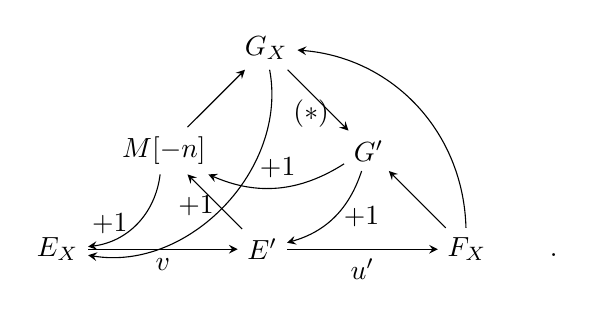
\begin{tikzpicture}[>=stealth,baseline=(GX.base),node distance=1.0cm]
  \node (EX) at (0,0) {$E_X$};
  \node (Ep) at (2.6,0) {$E'$};
  \node (FX) at (5.2,0) {$F_X$};
  \node (M)  at (1.35,1.25) {$M[-n]$};
  \node (GX) at (2.65,2.55) {$G_X$};
  \node (Gp) at (3.95,1.25) {$G'$};
  \node at (3.22,1.72) {$(*)$};
  \draw[->] (EX) -- node[below] {$v$} (Ep);
  \draw[->] (Ep) -- node[below] {$u'$} (FX);
  \draw[->] (Ep) -- (M);
  \draw[->] (M) -- (GX);
  \draw[->] (GX) -- (Gp);
  \draw[->] (FX) -- (Gp);
  \draw[->] (M) to[bend left=38] node[left] {$+1$} (EX);
  \draw[->] (Gp) to[bend left=28] node[above] {$+1$} (M);
  \draw[->] (Gp) to[bend left=28] node[right] {$+1$} (Ep);
  \draw[->] (GX) to[bend left=55] node[left] {$+1$} (EX);
  \draw[->] (FX) to[bend right=42] (GX);
  \node[anchor=base] at (6.3,0 |- FX.base) {.};
\end{tikzpicture}
\]
La suite exacte de cohomologie du triangle distingué \((*)\) montre que \(\Ho^n(G_X)\longrightarrow \Ho^n(G')\) est un épimorphisme, donc que \(\Ho^n(G')\) est bien de \(\underline{C}_0\)-type fini.

La correction précédente nous ramène donc au cas où \(\Ho^{n+1}(u)\) est un monomorphisme, ce que nous supposerons maintenant. La suite exacte de cohomologie de \(E\to F\to G\) donne alors une suite exacte
\begin{equation}\tag{.}
  \Ho^n(E)\xrightarrow{\Ho^n(u)}
  \Ho^n(F)\longrightarrow \Ho^n(G)\longrightarrow 0.
\end{equation}
Comme \(\Ho^n(G)\) est de \(\underline{C}_0\)-type fini, l'ensemble des \(X\) au-dessus de \(S\) tels qu'il existe un épimorphisme \(M\longrightarrow \Ho^n(G_X)\) avec \(M\in\Ob\underline{C}_{0X}\) est, par définition, un raffinement de \(S\). Utilisant la quasi-relevabilité de \(\underline{C}_0\) dans \(\underline{C}\), on peut imposer que cet épimorphisme se factorise à travers \(Z^n(F_X)\) en
\[
  M\xrightarrow{s}Z^n(F_X)\longrightarrow \Ho^n(F_X)\longrightarrow \Ho^n(G_X).
\]
Il est clair que \(u'\), défini comme en (1.4.1) avec \((r=0)\), est un morphisme de complexes et que \(\Ho^{n+1}(u')=\Ho^{n+1}(u_X)\). D'autre part, il est immédiat, à partir de la suite exacte (.), que
%%%%%%%%%%  scan idx 106  |  folio 93  %%%%%%%%%%
\[
  \Ho^n(u'):\Ho^n(E_X)\oplus M\longrightarrow \Ho^n(F_X)
\]
est un
épimorphisme. Cela termine la démonstration de (1.4.1).

\textbf{Lemme 1.4.2.} \uline{Soient} \(\underline{C}\) \uline{une catégorie abélienne,} \(u:E\to F\) \uline{un morphisme de complexes de} \(\underline{C}\) \uline{(resp.\ une flèche de} \(\Dpx(\underline{C})\)\uline{),} \(G\) \uline{le cône de} \(u\)\uline{. Conditions équivalentes pour} \(n\in\mathbb Z\) \uline{donné} :
\begin{enumerate}[label=(\roman*)]
\item \(\Ho^i(G)=0\) \uline{pour} \(i\geq n\)~;
\item \(\Ho^i(u)\) \uline{est un isomorphisme pour} \(i>n\) \uline{et un épimorphisme pour} \(i=n\).
\end{enumerate}
La preuve est immédiate à partir de la suite exacte de cohomologie.

\textbf{Définition 1.4.3.} \uline{Nous dirons que} \(u\) \uline{est un} \(n\)-quasi-isomorphisme (\uline{resp.\ un} \(n\)-isomorphisme) \uline{si} \(u\) \uline{vérifie les conditions équivalentes de (1.4.2).}

Cela étant, on déduit aussitôt de (1.4.1) le

\textbf{Corollaire 1.4.4.} \uline{Soient} \(\underline{S},S,\underline{C},\underline{C}_0\) \uline{comme en (1.4.1). Soit} \(u:E\to F\) \uline{un} \((n+1)\)\uline{-quasi-isomorphisme de complexes de} \(\underline{C}_S\) \uline{(}\(n\in\mathbb Z\) \uline{donné) tel que} \(\Ho^n(G)\) \uline{soit de} \(\underline{C}_0\)\uline{-type fini. Alors l'ensemble des} \(X\) \uline{au-dessus de} \(S\) \uline{tels qu'il existe} \((M,r,s)\) \uline{comme en (1.4.1) tels que} \(u'\) \uline{soit un} \(n\)\uline{-quasi-isomorphisme est un raffinement de} \(S\)\uline{.}

De manière imagée, on peut, moyennant la condition de finitude sur \(\Ho^n(G)\), localement «~gagner un cran~», i.e. modifier localement \(u\) en degré \(n\) par l'addition à \(E^n\) d'un objet de \(\underline{C}_0\) de manière à faire de \(u\) un \(n\)-quasi-isomorphisme.

\textbf{Corollaire 1.4.5.} \uline{Soient} \(\underline{C}\) \uline{une catégorie abélienne,} \(n\in\mathbb Z\)\uline{, et} \(u:E\to F\) \uline{un} \(n\)\uline{-quasi-isomorphisme de complexes de} \(\underline{C}\)\uline{. Il existe un diagramme commutatif de} \(\Cpx(\underline{C})\)
\[
\begin{tikzcd}
E \arrow[r,"v"] \arrow[d,"u"'] & E' \arrow[dl,"u'"]\\
F & ,
\end{tikzcd}
\]
%%%%%%%%%%  scan idx 107  |  folio 94  %%%%%%%%%%
\uline{où} \(u'\) \uline{est un
quasi-isomorphisme et} \(v\) \uline{un monomorphisme induisant l'identité en degré} \(\geq n\) (i.e. tel que \(E'^i=E^i\) et \(v^i=\id(E^i)\) pour \(i\geq n\)).

\uline{Preuve.} Appliquant (1.4.4) dans le cas où \(\underline{S}\) est le site ponctuel et \(\underline{C}_0=\underline{C}\), on obtient un triangle commutatif de \(\Cpx(\underline{C})\)
\[
\begin{tikzcd}
E \arrow[r,"v_{n-1}"] \arrow[d,"u"'] & E'_{\,n-1} \arrow[dl,"u'_{n-1}"]\\
F & ,
\end{tikzcd}
\]
où \(u'_{n-1}\) est un \((n-1)\)-quasi-isomorphisme et \(v_{n-1}\) un monomorphisme induisant l'identité en degré \(\geq n\). Itérant le procédé, on trouve, pour \(i\leq n-1\), une suite de triangles commutatifs de \(\Cpx(\underline{C})\)
\[
\begin{tikzcd}
E'_i \arrow[r,"v_{i-1}"] \arrow[d,"u'_i"'] & E'_{\,i-1} \arrow[dl,"u'_{i-1}"]\\
F & ,
\end{tikzcd}
\]
où \(u'_i\) est un \(i\)-quasi-isomorphisme et \(v_{i-1}\) un monomorphisme induisant l'identité en degré \(\geq i\). Le corollaire s'en déduit par passage à la limite. De manière précise, notant \(d'_i\) la différentielle de \(E'_i\), on définit \(E'\) par
\[
  E'^i=E^i,\quad d'^i=d^i\quad\text{pour }i\geq n,
\]
et
\[
  E'^i=(E'_i)^i,\quad d'^i=(d'_i)^i\quad\text{pour }i<n,
\]
puis \(v\) et \(u'\) par
\[
  v^j=(v_i v_{i+1}\ldots v_{n-1})^j,\qquad u'^j=(u'_i)^j\qquad\text{pour }i\leq j,
\]
et l'on vérifie aussitôt que \(E'\), \(v\), \(u'\) ainsi définis répondent à la question.

%%%%%%%%%%  scan idx 108  |  folio 95  %%%%%%%%%%
Autrement dit, en abrégé, on peut prolonger un \(n\)-quasi-isomorphisme en un quasi-isomorphisme «~sans rien changer à ce qui est donné en degré \(\geq n\)~».

\section*{2. Complexes pseudo-cohérents}

2.0. Dans ce numéro, \(\underline{S}\) désigne un site, \(S\) un objet de \(\underline{S}\), \(\underline{C}\) une \(\underline{S}\)-catégorie abélienne plate (1.1), \(\underline{C}_0\) une sous-\(\underline{S}\)-catégorie additive strictement pleine de \(\underline{C}\). On suppose que \(\underline{C}_0\) est localement quasi-stable par noyau d'épimorphisme (1.2) et localement quasi-relevable dans \(\underline{C}\) (1.2).

\textbf{Définition 2.1.} \uline{Soient} \(X\in\Ob \underline{S}\)\uline{,} \(E\) \uline{un complexe de} \(\underline{C}_X\)\uline{, et} \(n\in\mathbb Z\)\uline{. Nous dirons que} \(E\) \uline{est} strictement \(\underline{C}_0\)-\(n\)-pseudo-cohérent (resp.\ \(\underline{C}_0\)-pseudo-cohérent, resp.\ \(\underline{C}_0\)-parfait) \uline{si} \(E^i=0\) \uline{pour} \(i\) \uline{assez grand et} \(E^i\in\Ob\underline{C}_{0X}\) \uline{pour} \(i\geq n\) \uline{(resp.\ pour tout} \(i\)\uline{, resp.\ pour tout} \(i\) \uline{et} \(E^i=0\) \uline{pour presque tout} \(i\)\uline{).}

Quand il n'y aura pas de confusion à craindre, nous dirons parfois «~strictement \(n\)-pseudo-cohérent (resp\dots)~» au lieu de «~strictement \(\underline{C}_0\)-\(n\)-pseudo-cohérent (resp\dots)~».

\textbf{Lemme 2.1.1.} \uline{Soient} \(E\in\Ob\Cpx(\underline{C}_S)\) \uline{et} \(n\in\mathbb Z\)\uline{. Si} \(E\) \uline{est strictement} \(n\)\uline{-pseudo-cohérent et si} \(\Ho^i(E)=0\) \uline{pour} \(i>n\)\uline{, alors} \(\Ho^n(E)\) \uline{est de type fini.}

\uline{Preuve.} La suite
\[
  0\longrightarrow Z^n(E)\longrightarrow E^n\longrightarrow E^{n+1}\longrightarrow\ldots\longrightarrow 0
\]
est exacte et \(E^i\in\Ob\underline{C}_0\) pour \(i\geq n\). Comme \(\underline{C}_0\) est localement quasi-stable par noyau d'épimorphisme, il s'ensuit que \(Z^n(E)\) est de type fini, donc aussi \(\Ho^n(E)\), qui en est un quotient.

%%%%%%%%%%  scan idx 109  |  folio 96  %%%%%%%%%%
\textbf{Proposition 2.2.} \uline{Soient} \(F\in\Ob\Dpx(\underline{C}_S)\) \uline{et} \(n\in\mathbb Z\)\uline{. Alors} :

a) \uline{Si} \(F\) \uline{est strictement} \(n\)\uline{-pseudo-cohérent (relativement à} \(\underline{C}_0\)\uline{) et si} \(u:E\to F\) \uline{est un quasi-isomorphisme, l'ensemble des} \(X\) \uline{au-dessus de} \(S\) \uline{tels qu'il existe un quasi-isomorphisme} \(v:F'\longrightarrow E_X\) \uline{avec} \(F'\) \uline{strictement} \(n\)\uline{-pseudo-cohérent est un raffinement de} \(S\)\uline{.}

b) \uline{Les conditions suivantes sont équivalentes} :
\begin{enumerate}[label=(\roman*)]
\item \uline{l'ensemble des} \(X\) \uline{au-dessus de} \(S\) \uline{tels qu'il existe un quasi-isomorphisme} \(u:E\longrightarrow F_X\) \uline{de} \(\Cpx(\underline{C}_X)\)\uline{, avec} \(E\) \uline{strictement} \(n\)\uline{-pseudo-cohérent, est un raffinement de} \(S\)~;
\item[\((\mathrm{i}')\)] \uline{même condition que (i), mais} \(u\) \uline{étant un isomorphisme de} \(\Dpx(\underline{C}_X)\)~;
\item \uline{l'ensemble des} \(X\) \uline{au-dessus de} \(S\) \uline{tels qu'il existe un} \(n\)\uline{-quasi-isomorphisme (1.4.3)} \(u:E\longrightarrow F_X\) \uline{de} \(\Cpx(\underline{C}_X)\)\uline{, avec} \(E\) \uline{strictement parfait, est un raffinement de} \(S\)~;
\item[\((\mathrm{ii}')\)] \uline{même condition que (ii), mais} \(u\) \uline{étant un} \(n\)\uline{-isomorphisme de} \(\Dpx(\underline{C}_X)\).
\end{enumerate}

\uline{Démonstration.} a) Il existe, pour un entier \(i\) assez grand, un \(i\)-quasi-isomorphisme \(v_i:F'_i\longrightarrow E\), avec \(F'_i\) strictement \(n\)-pseudo-cohérent (prendre \(F'_i=0\)). Montrons que, si \(i>n\), il existe, quitte à raffiner \(S\), un \((i-1)\)-quasi-isomorphisme \(v_{i-1}:F'_{i-1}\longrightarrow E\), avec \(F'_{i-1}\) strictement \(n\)-pseudo-cohérent. D'après (1.4.4), il suffit de montrer que \(\Ho^{i-1}(M')\), où \(M'\) est le cône de \(v_i\), est de \(\underline{C}_0\)-type fini. Or, si \(M''\) désigne le cône de \(uv_i\), l'hypothèse que \(u\) est un quasi-isomorphisme et (1.4.2) impliquent que l'on a
\[
  \Ho^j(M')\qis \Ho^j(M'')\qquad\text{pour tout }j
\]
et \(\Ho^j(M')=0\) pour \(j\geq i\).
%%%%%%%%%%  scan idx 110  |  folio 97  %%%%%%%%%%
La
formule du cône \(M''{}^j=F'_i{}^{\,j+1}\oplus F^j\) montre d'autre part que \(M''\) est strictement \((i-1)\)-pseudo-cohérent. Donc, en vertu de (2.1.1), \(\Ho^{i-1}(M'')=\Ho^{i-1}(M')\) est de type fini, d'où notre assertion. On en déduit, par itération, et quitte à raffiner \(S\), un \(n\)-quasi-isomorphisme \(v_n:F'_n\longrightarrow E\), où \(F'_n\) est strictement \(n\)-pseudo-cohérent. Mais, d'après (1.4.5), on peut prolonger \(v_n\) en un quasi-isomorphisme \(v:F'\longrightarrow E\) sans rien changer en degré \(\geq n\), donc en particulier avec \(F'\) strictement \(n\)-pseudo-cohérent, ce qui prouve a).

b) L'équivalence des conditions (i) et \((\mathrm{i}')\) résulte aussitôt de a) et de la définition des isomorphismes de \(\Dpx^-(\underline{C}_X)\). Si \(E\in\Ob\Dpx^-(\underline{C}_S)\) est strictement \(n\)-pseudo-cohérent, il existe une suite exacte
\[
  0\longrightarrow E'\longrightarrow E\longrightarrow E''\longrightarrow 0,
\]
où \(E'\) est strictement parfait, et \(E''{}^i=0\) pour \(i\geq n\); par suite \(E'\to E\) est un \(n\)-quasi-isomorphisme, d'où l'implication \((\mathrm{i})\Rightarrow(\mathrm{ii})\). L'implication \((\mathrm{ii})\Rightarrow(\mathrm{ii}')\) étant triviale, il reste à prouver \((\mathrm{ii}')\Rightarrow(\mathrm{i})\). Soit donc \(u:E\longrightarrow F\) un \(n\)-isomorphisme de \(\Dpx^-(\underline{C}_S)\), avec \(E\) strictement parfait; \(u\) est donc défini par un diagramme de \(\Cpx^-(\underline{C}_S)\)
\[
\begin{tikzcd}
& E' \arrow[dl,"s"'] \arrow[dr,"u'"]\\
E && F ,
\end{tikzcd}
\]
où \(s\) est un quasi-isomorphisme et \(u'\) un \(n\)-quasi-isomorphisme. En vertu de a), il existe, quitte à raffiner \(S\), un quasi-isomorphisme \(t:E''\longrightarrow E'\), avec \(E''\) strictement \(n\)-pseudo-cohérent. On applique alors (1.4.5) pour prolonger \(u't:E''\to F\) en un quasi-isomorphisme \(E'''\longrightarrow F\) avec \(E'''\) strictement \(n\)-pseudo-cohérent, ce qui prouve \((\mathrm{ii}')\Rightarrow(\mathrm{i})\) et achève la démonstration de (2.2).

%%%%%%%%%%  scan idx 111  |  folio 98  %%%%%%%%%%
\textbf{Définition 2.3.} \uline{Sous les hypothèses de (2.2), nous dirons que} \(F\in\Ob\Dpx(\underline{C}_S)\) \uline{est} \(\underline{n}\)-\(\underline{C}_0\)-pseudo-cohérent \uline{si} \(F\) \uline{vérifie les conditions équivalentes b) de (2.2). Nous dirons que} \(F\) \uline{est} \(\underline{C}_0\)-pseudo-cohérent \uline{si} \(F\) \uline{est} \(n\)\uline{-}\(\underline{C}_0\)\uline{-pseudo-cohérent pour tout} \(n\)\uline{.}

Quand cela ne pourra prêter à confusion, nous nous permettrons parfois de dire \(n\)-pseudo-cohérent, pseudo-cohérent, au lieu de \(n\)-\(\underline{C}_0\)-pseudo-cohérent, \(\underline{C}_0\)-pseudo-cohérent.

\textbf{Remarque 2.3.1.} Soit \(F\in\Ob\Dpx(\underline{C}_S)\) un complexe pseudo-cohérent. L'ensemble des \(X\) au-dessus de \(S\) tels qu'il existe un quasi-isomorphisme \(E\longrightarrow F_X\) avec \(E\) strictement pseudo-cohérent (2.1) n'est pas en général un raffinement de \(S\). Toutefois, nous verrons plus tard (2.7. a) et Exp.II) des cas importants où il en est ainsi.

La démonstration de (2.2 a)) donne le résultat suivant :

\textbf{Proposition 2.4.} \uline{Soient} \(n,i\in\mathbb Z\)\uline{, et soit} \(u:E\to F\) \uline{un} \(i\)\uline{-quasi-isomorphisme de} \(\Cpx(\underline{C}_S)\)\uline{, avec} \(F\) \(n\)\uline{-pseudo-cohérent et} \(E\) \uline{strictement} \(n\)\uline{-pseudo-cohérent. Alors, quitte à raffiner} \(S\)\uline{, il existe un triangle commutatif de} \(\Cpx(\underline{C}_S)\)
\[
\begin{tikzcd}
E \arrow[r,"v"] \arrow[d,"u"'] & E' \arrow[dl,"u'"]\\
F & ,
\end{tikzcd}
\]
\uline{où} \(E'\) \uline{est strictement} \(n\)\uline{-pseudo-cohérent,} \(u'\) \uline{un quasi-isomorphisme et} \(v\) \uline{un monomorphisme induisant l'identité en degré} \(\geq i\)\uline{.}

\textbf{Proposition 2.5.} a) \uline{Si} \(F\in\Ob\Dpx(\underline{C}_S)\) \uline{est} \(n\)\uline{-pseudo-cohérent (resp. pseudo-cohérent),} \(F[m]\) \uline{est} \((n-m)\)\uline{-pseudo-cohérent (resp. pseudo-cohérent).}

%%%%%%%%%%  scan idx 112  |  folio 99  %%%%%%%%%%
b) \uline{Soit}
\[
\begin{tikzcd}
& G \arrow[dl,"+1"'] & \\
E \arrow[rr] && F \arrow[ul]
\end{tikzcd}
\tag{*}
\]
\uline{un
triangle distingué de} \(\Dpx(\underline{C}_S)\)\uline{. Si} \(E\) \uline{et} \(G\) \uline{sont} \(n\)\uline{-pseudo-cohérents (resp. pseudo-cohérents), alors} \(F\) \uline{est} \(n\)\uline{-pseudo-cohérent (resp. pseudo-cohérent).}

\uline{Preuve.} a) Trivial à partir des définitions.

b) Il suffit bien entendu de démontrer l'assertion non respée. Le triangle \((*)\) peut encore s'écrire
\[
\begin{tikzcd}
& F \arrow[dl,"+1"'] & \\
G[-1] \arrow[rr] && E \arrow[ul] & .
\end{tikzcd}
\]
D'après a), \(G[-1]\) est \((n+1)\)-pseudo-cohérent. On est donc ramené à prouver que, si \(E\) est \((n+1)\)-pseudo-cohérent et \(F\) \(n\)-pseudo-cohérent, alors \(G\) est \(n\)-pseudo-cohérent. Quitte à se localiser, on peut supposer \(E\) (resp. \(F\)) strictement \((n+1)\)-pseudo-cohérent (resp. \(n\)-pseudo-cohérent). La flèche \(E\xrightarrow{u}F\) de \(\Dpx^-(\underline{C}_S)\) est définie par un couple de flèches de \(\Cpx^-(\underline{C}_S)\)
\[
\begin{tikzcd}
& E' \arrow[dl,"s"'] \arrow[dr,"u'"]\\
E && F ,
\end{tikzcd}
\]
où \(s\) est un quasi-isomorphisme. D'après (2.2 a)), il existe, quitte à localiser, un quasi-isomorphisme \(t:E''\to E'\), où \(E''\) est strictement \((n+1)\)-pseudo-cohérent. On est donc réduit au cas où \(u\) est définie par une 
%%%%%%%%%%  scan idx 113  |  folio 100  %%%%%%%%%%
«
vraie » flèche de \(\Cpx^-(\underline{C}_S)\). L'assertion résulte alors des définitions et de la formule \(C(u)^i=E^{i+1}\oplus F^i\), où \(C(u)\) désigne le cône de \(u\).

\textbf{Scholie 2.6.} Par « rotation » des triangles, on voit que des propriétés de pseudo-cohérence sur deux des objets du triangle \((*)\) en impliquent une autre sur le troisième. On peut résumer les différents cas dans le tableau ci-dessous (les petites lettres désignent des degrés de pseudo-cohérence et chaque ligne correspond à une implication dont le but est souligné) :
\[
\begin{array}{ccc}
E&F&G\\[0.2em]
n+1&n&\underline n\\
n&\underline n&n\\
\underline n&n&n-1 .
\end{array}
\]

Nous noterons \(\Dpx(\underline{C})_{\underline{C}_0\text{-}n\text{-coh}}\) (resp. \(\Dpx(\underline{C})_{\underline{C}_0\text{-}\mathrm{coh}}\)) la sous-catégorie fibrée strictement pleine de \(\Dpx(\underline{C})\) dont la fibre en chaque \(X\in\Ob \underline{S}\) est formée des objets de \(\Dpx(\underline{C}_X)\) qui sont \(n\)-pseudo-cohérents (resp. pseudo-cohérents) relativement à \(\underline{C}_0\). La catégorie \(\Dpx(\underline{C})_{\underline{C}_0\text{-}\mathrm{coh}}\) est, en vertu de (2.5), une sous-\(\underline{S}\)-\uline{catégorie triangulée} de \(\Dpx(\underline{C})\) (1.1).

\textbf{Proposition 2.7.} \uline{Supposons que} \(\underline{S}\) \uline{soit un site ponctuel, donc} \(\underline{C}=\underline{C}_S\)\uline{,} \(\underline{C}_0=\underline{C}_{0S}\)\uline{. Alors} :

a) \uline{Si} \(F\in\Ob\Dpx(\underline{C})\) \uline{est pseudo-cohérent, il existe un quasi-isomorphisme} \(E\longrightarrow F\)\uline{, avec} \(E\) \uline{strictement pseudo-cohérent} (2.1).

b) \uline{Désignons par} \(\Kpx^{-,\varnothing}(\underline{C}_0)\) \uline{la sous-catégorie triangulée pleine de} \(\Kpx^-(\underline{C}_0)\) \uline{formée des complexes acycliques. Le foncteur canonique}
\[
  \Kpx^-(\underline{C}_0)/\Kpx^{-,\varnothing}(\underline{C}_0)
  \longrightarrow \Dpx(\underline{C})
\]
%%%%%%%%%%  scan idx 114  |  folio 101  %%%%%%%%%%
\uline{est
pleinement fidèle et a pour image essentielle} \(\Dpx(\underline{C})_{\underline{C}_0\text{-}\mathrm{coh}}\).

\uline{Preuve.} a) Soit \(F\in\Ob\Dpx(\underline{C})_{\underline{C}_0\text{-}\mathrm{coh}}\), et supposons construit un \(i\)-quasi-isomorphisme (de \(\Cpx(\underline{C})\)) \(u_i:E_i\longrightarrow F\) avec \(E_i\) strictement pseudo-cohérent (c'est possible pour \(i\) assez grand avec \(E_i=0\)). Soit \(G_i\) le cône de \(u_i\). Il résulte de (1.4.2) et (2.1.1) que \(\Ho^{i-1}(G_i)\) est de \(\underline{C}_0\)-type fini. Donc, en vertu de (1.4.4), il existe un triangle commutatif de \(\Cpx(\underline{C})\)
\[
\begin{tikzcd}
E_i \arrow[r,"v_{i-1}"] \arrow[d,"u_i"'] & E_{i-1} \arrow[dl,"u_{i-1}"]\\
F & ,
\end{tikzcd}
\]
où \(E_{i-1}\) est strictement pseudo-cohérent, \(u_{i-1}\) un \((i-1)\)-quasi-isomorphisme, et \(v_{i-1}\) un monomorphisme induisant l'identité en degré \(\geq i\). On en déduit par passage à la limite (cf. preuve de (1.4.5)) un quasi-isomorphisme \(u:E\to F\) avec \(E\) strictement pseudo-cohérent.

b) Appliquer le critère ([V] chap I § 2 4.2 b)(i)) et a).

Noter que la preuve de a) donne le résultat plus précis suivant, qui généralise (1.4.5) :

\textbf{Proposition 2.7.1.} \uline{Sous les hypothèses de (2.7), soit} \(u:E\to F\) \uline{un} \(n\)\uline{-quasi-isomorphisme de} \(\Cpx(\underline{C})\)\uline{, avec} \(F\) \uline{pseudo-cohérent et} \(E\) \uline{strictement pseudo-cohérent. Il existe alors un triangle commutatif de} \(\Cpx(\underline{C})\)
\[
\begin{tikzcd}
E \arrow[r,"v"] \arrow[d,"u"'] & E' \arrow[dl,"u'"]\\
F & ,
\end{tikzcd}
\]
\uline{où} \(E'\) \uline{est strictement pseudo-cohérent,} \(u'\) \uline{un quasi-isomorphisme, et} \(v\) \uline{un}
%%%%%%%%%%  scan idx 115  |  folio 102  %%%%%%%%%%
\uline{monomorphisme induisant l'identité en degré} \(\geq n\).

\textbf{Définition 2.8.} \uline{Soient} \(n\in\mathbb N\) \uline{et} \(F\in\Ob\underline{C}_S\)\uline{. Nous dirons que} \(F\) \uline{est de} \(\underline{n}\)-\(\underline{C}_0\)-présentation finie \uline{si l'ensemble des} \(X\) \uline{au-dessus de} \(S\) \uline{tels qu'il existe une suite exacte}
\[
  E^{-n}\longrightarrow\ldots\longrightarrow E^0\longrightarrow F_X\longrightarrow 0,
\]
\uline{avec} \(E^i\in\Ob\underline{C}_{0X}\) \uline{pour} \(-n\leq i\leq 0\)\uline{, est un raffinement de} \(S\)\uline{. Nous dirons que} \(F\) \uline{est d'}\(\infty\)-\(\underline{C}_0\)-présentation finie \uline{si} \(F\) \uline{est de} \(n\)\uline{-}\(\underline{C}_0\)\uline{-présentation finie pour tout} \(n\in\mathbb N\).

Bien entendu, nous dirons parfois \(n\)-présentation finie tout court quand il n'y aura pas d'ambiguïté possible sur \(\underline{C}_0\).

Nous dirons « de présentation finie » pour « de 1-présentation finie », et « de type fini » pour « de 0-présentation finie », cette dernière notion coïncidant avec celle déjà introduite en (1.2).

\textbf{Proposition 2.9.} \uline{Soient} \(n\in\mathbb N\) \uline{et} \(F\in\Ob\underline{C}_S\)\uline{. Conditions équivalentes} :

(i) \(F\) \uline{est de} \(n\)\uline{-présentation finie (resp. d'}\(\infty\)\uline{-présentation finie)};

(ii) \(F\) \uline{est} \((-n)\)\uline{-pseudo-cohérent (resp. pseudo-cohérent)}.

\uline{Dans le cas où} \(\underline{S}\) \uline{est un site ponctuel,} \(F\) \uline{est pseudo-cohérent si et seulement s'il existe une suite exacte}
\[
  \ldots\longrightarrow E^i\longrightarrow\ldots\longrightarrow E^0\longrightarrow F\longrightarrow 0,
\]
\uline{avec} \(E^i\in\Ob\underline{C}_0\) \uline{pour tout} \(i\).

\uline{Preuve.} Pour l'équivalence \((\mathrm{i})\Leftrightarrow(\mathrm{ii})\), il suffit évidemment de traiter le cas non respé. L'implication \((\mathrm{i})\Rightarrow(\mathrm{ii})\) est immédiate sur les définitions, et 
%%%%%%%%%%  scan idx 116  |  folio 103  %%%%%%%%%%
l'%
implication \((\mathrm{ii})\Rightarrow(\mathrm{i})\) résulte aussitôt de (2.4) : la flèche \(0\to F\) est un 1-quasi-isomorphisme, on en déduit (quitte à localiser) un quasi-isomorphisme \(E\longrightarrow F\) avec \(E\) strictement \((-n)\)-pseudo-cohérent et \(E^i=0\) pour \(i\geq 1\), i.e. une \(n\)-présentation finie de \(F\). La deuxième assertion se démontre de manière analogue (utiliser (2.7.1)).

\textbf{Proposition 2.10.} a) \uline{Soient} \(m,n\in\mathbb Z\)\uline{, avec} \(n\leq m\)\uline{. Si} \(F\in\Ob\Dpx^-(\underline{C}_S)\) \uline{est} \(n\)\uline{-pseudo-cohérent et acyclique en degré} \(\geq m\)\uline{, il existe localement un quasi-isomorphisme} \(E\longrightarrow F\)\uline{, avec} \(E\) \uline{strictement} \(n\)\uline{-pseudo-cohérent et} \(E^i=0\) \uline{pour} \(i\geq m\)\uline{. Si} \(\underline{S}\) \uline{est ponctuel, et} \(F\) \uline{pseudo-cohérent et acyclique en degré} \(\geq m\)\uline{, il existe un quasi-isomorphisme} \(E\longrightarrow F\) \uline{avec} \(E\) \uline{strictement pseudo-cohérent et} \(E^i=0\) \uline{pour} \(i\geq m\)\uline{.}

b) \uline{Soit} \(F\in\Ob\Dpx^-(\underline{C}_S)\) \uline{acyclique en degré} \(>n\)\uline{. Pour que} \(F\) \uline{soit} \(n\)\uline{-pseudo-cohérent, il faut et il suffit que} \(\Ho^n(F)\) \uline{soit de type fini.}

\uline{Preuve.} a) Comme \(F\) est acyclique en degré \(\geq m\), la flèche \(0\to F\) est un \(m\)-quasi-isomorphisme. L'assertion résulte de (2.4) et (2.7.1).

b) Il existe un triangle distingué de \(\Dpx^-(\underline{C}_S)\) :
\[
\begin{tikzcd}
& F' \arrow[dl,"+1"'] & \\
F \arrow[rr] && \Ho^n(F)[-n] \arrow[ul] & ,
\end{tikzcd}
\]
(pour le voir, commencer par tronquer \(F\) en remplaçant \(F^n\) par \(Z^n(F)\) et \(F^i\) par \(0\) pour \(i>n\)). La suite exacte de cohomologie implique \(\Ho^i(F')=0\) pour \(i\geq n-1\), donc \(F'\) est \((n-1)\)-pseudo-cohérent. On conclut grâce à (2.5) et (2.6).



% Additional notation for Expose I continuation
\providecommand{\RHom}{\mathrm R\!\Hom}
\providecommand{\Ext}{\operatorname{Ext}}
\providecommand{\coh}{\operatorname{coh}}
\providecommand{\PreCoh}{\operatorname{precoh}}
\providecommand{\Tr}{\operatorname{Tr}}
\providecommand{\Qis}{\operatorname{Qis}}
\providecommand{\Rad}{\operatorname{rad}}
\providecommand{\Spec}{\operatorname{Spec}}
\providecommand{\End}{\operatorname{End}}
\providecommand{\Id}{\operatorname{Id}}
\providecommand{\varinjlim}{\mathop{\mathrm{lim}}\limits_{\longrightarrow}}
\providecommand{\varprojlim}{\mathop{\mathrm{lim}}\limits_{\longleftarrow}}
\providecommand{\qcoh}{\operatorname{qcoh}}
\providecommand{\amp}{\operatorname{amp}}


%%%%%%%%%%  scan idx 117  |  folio 104  %%%%%%%%%%
\textbf{Proposition 2.11.} \uline{Soit} \(n\in\mathbb Z\)\uline{.}

a) \uline{Soit} \(F\in\Ob\Cpx^-(\underline{C}_S)\)\uline{. Si, pour tout} \(i\geq n\) \uline{(resp. pour tout} \(i\)\uline{),} \(F^i\) \uline{est de} \((i-n)\)\uline{-présentation finie (resp. d'}\(\infty\)\uline{-présentation finie), alors} \(F\) \uline{est} \(n\)\uline{-pseudo-cohérent (resp. pseudo-cohérent).}

b) \uline{Soit} \(F\in\Ob\Dpx^-(\underline{C}_S)\)\uline{. Si, pour tout} \(i\geq n\) \uline{(resp. pour tout} \(i\)\uline{),} \(\Ho^i(F)\) \uline{est de} \((i-n)\)\uline{-présentation finie (resp. d'}\(\infty\)\uline{-présentation finie), alors} \(F\) \uline{est} \(n\)\uline{-pseudo-cohérent (resp. pseudo-cohérent).}

\uline{Preuve.} Il suffit de traiter les assertions non respées.

a) On raisonne par récurrence sur \(N\) tel que \(F^i=0\) pour \(i>n+N\). Si \(N=0\), l'assertion résulte aussitôt de (2.10 b)). Supposons \(N\geq1\). On a une suite exacte
\[
  0\longrightarrow F^{n+N}[-n-N]\longrightarrow F\longrightarrow F'\longrightarrow 0,
\]
Par hypothèse de récurrence, \(F'\) est \(n\)-pseudo-cohérent; d'autre part, \(F^{n+N}[-n-N]\) est \(n\)-pseudo-cohérent par hypothèse (2.9 et 2.5.a)); donc, en vertu de (2.5.b)), \(F\) est \(n\)-pseudo-cohérent.

b) On raisonne par récurrence sur \(N\) tel que \(\Ho^i(F)=0\) pour \(i>n+N\). Si \(N=0\), l'assertion résulte de (2.10 b)). Supposons \(N\geq1\). On a un triangle distingué de \(\Dpx^-(\underline{C}_S)\) (cf. preuve de (2.10.b))) :
\[
\begin{tikzcd}
& F' \arrow[dl,"+1"'] & \\
F \arrow[rr] && \Ho^{n+N}(F)[-n-N] \arrow[ul] & .
\end{tikzcd}
\]
La suite exacte de cohomologie implique
\[
  \Ho^i(F')=0\quad\text{pour }i\geq n+N-1,\quad\text{i.e. }i>(n-1)+(N-1),
\]
et
\[
  \Ho^i(F')\qis\Ho^{i+1}(F)\quad\text{pour }i<n+N-1 .
\]
%%%%%%%%%%  scan idx 118  |  folio 105  %%%%%%%%%%
Par l'%
hypothèse de récurrence (appliquée pour \(n-1\) au lieu de \(n\)), \(F'\) est donc \((n-1)\)-pseudo-cohérent. D'autre part, \(\Ho^{n+N}(F)[-n-N]\) est \(n\)-pseudo-cohérent (2.9 et 2.5.a)). Donc, en vertu de (2.6), \(F\) est \(n\)-pseudo-cohérent.

\textbf{Remarque 2.11.1.} Si \(F\) est pseudo-cohérent, les \(F^i\) (resp. \(\Ho^i(F)\)) ne sont pas en général pseudo-cohérents, ni même de type fini. Toutefois, nous verrons au paragraphe suivant, dans les sorites sur les notions de cohérence, des exemples importants où la pseudo-cohérence de \(F\) implique celle des \(\Ho^i(F)\).

\textbf{Proposition 2.12.} \uline{Soient} \(F',F''\in\Ob\Dpx(\underline{C}_S)\)\uline{, et} \(F=F'+F''\)\uline{. Pour que} \(F\) \uline{soit} \(n\)\uline{-pseudo-cohérent (resp. pseudo-cohérent) il faut et il suffit que} \(F'\) \uline{et} \(F''\) \uline{soient} \(n\)\uline{-pseudo-cohérents (resp. pseudo-cohérents).}

\uline{Preuve.} Il suffit de prouver l'assertion non respée. La suffisance est évidente, prouvons la nécessité. On peut supposer, par récurrence, qu'on a déjà démontré que \(F'\) et \(F''\) sont \((n+1)\)-pseudo-cohérents. Quitte à se localiser, on peut même supposer que \(F'\) et \(F''\) sont strictement \((n+1)\)-pseudo-cohérents et que \(F=F'+F''\) dans \(\Cpx^-(\underline{C}_S)\). Notons \(F'_{>n}\) (resp. \(F'_{\leq n}\)) le complexe déduit de \(F'\) en remplaçant \(F'^i\) par \(0\) pour \(i\leq n\) (resp. \(i>n\)), et de même \(F''_{>n}\) (resp. \(F''_{\leq n}\))\dots{} On a une suite exacte
\[
  0\longrightarrow F'_{>n}+F''_{>n}\longrightarrow F
  \longrightarrow F'_{\leq n}+F''_{\leq n}\longrightarrow 0 .
\]
\(F'_{>n}+F''_{>n}\) est strictement parfait et \(F\) est \(n\)-pseudo-cohérent, donc (2.6) \(F'_{\leq n}+F''_{\leq n}\) est \(n\)-pseudo-cohérent. Cela signifie, d'après (2.10 b)), que \(\Ho^n(F'_{\leq n}+F''_{\leq n})\) est de type fini. Mais on a
\[
  \Ho^n(F'_{\leq n}+F''_{\leq n})
  =\Ho^n(F'_{\leq n})+\Ho^n(F''_{\leq n}),
\]
%%%%%%%%%%  scan idx 119  |  folio 106  %%%%%%%%%%
donc \(\Ho^n(F'_{\leq n})\) (resp. \(\Ho^n(F''_{\leq n})\)) est de type fini, donc à nouveau grâce à (2.10.b)) \(F'_{\leq n}\) (resp. \(F''_{\leq n}\)) est \(n\)-pseudo-cohérent. Appliquant (2.5) à la suite exacte
\[
  0\longrightarrow F'_{>n}\longrightarrow F'\longrightarrow F'_{\leq n}\longrightarrow 0,
\]
(resp.\dots), on en déduit que \(F'\) (resp. \(F''\)) est \(n\)-pseudo-cohérent, cqfd.

\textbf{Proposition 2.13.} \uline{Soit} \((\underline{S}',\underline{C}',\underline{C}'_0)\) \uline{un trio satisfaisant aux mêmes hypothèses} (2.0) \uline{que} \((\underline{S},\underline{C},\underline{C}_0)\)\uline{. Soit} \(f:\underline{S}'\to \underline{S}\) \uline{un morphisme de sites} ([G] I 1.4)\uline{, correspondant à un foncteur sous-jacent} \(f^{-1}:\underline{S}\to \underline{S}'\)\uline{, et soit}
\(u:\Dpx^*(\underline{C})\longrightarrow \Dpx^*(\underline{C}')\) \((*=+,-,\varnothing)\)
\uline{un foncteur cartésien au-dessus de} \(f\)\uline{,} i.e. \uline{un} \(\underline{S}\)\uline{-foncteur cartésien} \(\Dpx^*(\underline{C}')\times_{\underline{S}'}\underline{S}\longleftarrow\Dpx^*(\underline{C})\)\uline{. On suppose que} \(u\) \uline{est exact sur chaque fibre et qu'il existe} \(a,b\in\mathbb Z\) \uline{tels que les conditions suivantes soient vérifiées pour tout} \(S\in\Ob \underline{S}\) :

(i) \uline{si} \(E\in\Ob\underline{C}_{0S}\)\uline{,} \(u(E)\) \uline{est} \(a\)\uline{-}\(\underline{C}'_0\)\uline{-pseudo-cohérent (resp.} \(\underline{C}'_0\)\uline{-pseudo-cohérent)}

(ii) \uline{si} \(F\in\Ob\Dpx^*(\underline{C}_S)\) \uline{est acyclique en degré} \(>0\)\uline{,} \(u(F)\) \uline{est acyclique en degré} \(>b\)\uline{.}

\uline{Alors, si} \(F\in\Ob\Dpx^*(\underline{C}_S)\) \uline{est} \(m\)\uline{-pseudo-cohérent rel. à} \(\underline{C}_0\) \uline{et acyclique en degré} \(>n\)\uline{,} \(u(F)\in\Ob\Dpx^*(\underline{C}'_{S'})\) \uline{(où} \(S'=f^{-1}(S)\)\uline{) est} \(\sup(m+b,n+a)\)\uline{-pseudo-cohérent (rel. à} \(\underline{C}'_0\)\uline{) (resp.} \((m+b)\)\uline{-pseudo-cohérent) et acyclique en degré} \(>n+b\)\uline{.}

\uline{En particulier, dans le cas respé, si} \(F\in\Ob\Dpx^*(\underline{C}_S)\) \uline{est pseudo-cohérent} (rel. à \(\underline{C}_0\)), \(u(F)\) \uline{est pseudo-cohérent (rel. à} \(\underline{C}'_0\)\uline{).}

\uline{Preuve.} On peut se borner au cas non respé. Montrons d'abord que si \(F\in\Ob\Dpx^*(\underline{C}_S)\) est strictement parfait (2.1) et tel que \(F^i=0\) pour \(i>n\), alors \(u(F)\) est \((n+a)\)-\(\underline{C}'_0\)-pseudo-cohérent. Raisonnons par récurrence sur le nombre \(N\) d'indices \(i\) tels que \(F^i\neq0\). Si \(N=1\), 
%%%%%%%%%%  scan idx 120  |  folio 107  %%%%%%%%%%
on a \(F=F^p[-p]\)
pour un \(p\leq n\), donc \(u(F)\) est \((p+a)\)-\(\underline{C}'_0\)-pseudo-cohérent, donc a fortiori \((n+a)\)-pseudo-cohérent. Si \(N>1\), on a une suite exacte
\[
  0\longrightarrow F'\longrightarrow F\longrightarrow F''\longrightarrow 0,
\]
où \(F'\) et \(F''\) sont strictement parfaits de longueur \(\leq N-1\) et tels que \(F'^i=F''^i=0\) pour \(i>n\). Appliquant (2.5.b)) au triangle distingué
\[
\begin{tikzcd}
& u(F'') \arrow[dl,"+1"'] & \\
u(F') \arrow[rr] && u(F) \arrow[ul] & ,
\end{tikzcd}
\]
on déduit de l'hypothèse de récurrence que \(u(F)\) est \((n+a)\)-pseudo-cohérent.

Passons maintenant au cas général : \(F\) \(m\)-\(\underline{C}_0\)-pseudo-cohérent et acyclique en degré \(>n\). Quitte à localiser, on peut, grâce à (2.10.a)), supposer \(F\) strictement \(m\)-pseudo-cohérent et tel que \(F^i=0\) pour \(i>n\). On a alors une suite exacte
\[
  0\longrightarrow F'\longrightarrow F\longrightarrow F''\longrightarrow 0,
\]
où \(F''\) est nul en degré \(\geq m\) et \(F'\) strictement parfait et nul en degré \(>n\). Dans le triangle distingué
\[
\begin{tikzcd}
& u(F'') \arrow[dl,"+1"'] & \\
u(F') \arrow[rr] && u(F) \arrow[ul] & ,
\end{tikzcd}
\]
\(u(F'')\) est acyclique en degré \(\geq m+b\), donc \((m+b)\)-pseudo-cohérent, et \(u(F')\) est \((n+a)\)-pseudo-cohérent d'après ce qu'on a vu. On conclut par (2.5.b)).

\textbf{Corollaire 2.14.} \uline{Soit} \(\underline{C}_1\) \uline{une sous-}\(\underline{S}\)\uline{-catégorie additive strictement pleine de} \(\underline{C}\) \uline{telle que} \(\underline{C}_0\subset\underline{C}_1\subset\underline{C}\)\uline{. On suppose que tout objet de} \(\underline{C}_1\) \uline{est} \(\underline{C}_0\)\uline{-pseudo-cohérent.}
%%%%%%%%%%  scan idx 121  |  folio 108  %%%%%%%%%%
\uline{Alors} :

(i) \(\underline{C}_1\) \uline{est localement quasi-relevable dans} \(\underline{C}\) (1.2) \uline{et localement quasi-stable par noyau d'épimorphisme} (1.2)\uline{.}

(ii) \uline{Soient} \(S\in\Ob \underline{S}\) \uline{et} \(F\in\Ob\Dpx(\underline{C}_S)\)\uline{. Pour que} \(F\) \uline{soit} \(n\)\uline{-pseudo-cohérent (resp. pseudo-cohérent) relativement à} \(\underline{C}_1\)\uline{, il faut et il suffit qu'il le soit relativement à} \(\underline{C}_0\)\uline{.}

\uline{Preuve.} (i) Soit \(E\to F\) un épimorphisme de \(\underline{C}_S\), avec \(F\in\Ob\underline{C}_{1S}\). Comme \(F\) est \(\underline{C}_0\)-pseudo-cohérent (donc a fortiori de \(\underline{C}_0\)-type fini), il existe (quitte à localiser) un épimorphisme \(E'\to F\) avec \(E'\in\Ob\underline{C}_{0S}\). Utilisant la quasi-relevabilité de \(\underline{C}_0\) dans \(\underline{C}\), on peut supposer (quitte à localiser à nouveau) que celui-ci se factorise à travers \(E\), d'où la quasi-relevabilité de \(\underline{C}_1\). D'autre part, si \(E\in\Ob\underline{C}_S\) admet une résolution droite finie par des objets de \(\underline{C}_1\), \(E\) est \(\underline{C}_0\)-pseudo-cohérent en vertu de (2.11.a)), donc a fortiori de \(\underline{C}_1\)-type fini.

(ii) Il suffit de prouver la nécessité. On peut pour cela appliquer, au choix, (2.11.a)) ou (2.13) avec \(\underline{S}'=\underline{S}\), \(\underline{C}'=\underline{C}\), \(f=\text{Identité}\), \(u=\text{Identité}\), \(\underline{C}'_0\) et \(\underline{C}_0\) remplacées respectivement par \(\underline{C}_0\) et \(\underline{C}_1\).

\textbf{Scholie 2.14.1.} Il existe donc une plus grande sous-\(\underline{S}\)-catégorie additive strictement pleine de \(\underline{C}\) donnant la même notion de \(n\)-pseudo-cohérence (resp. pseudo-cohérence) que \(\underline{C}_0\), à savoir la catégorie formée des objets \(\underline{C}_0\)-pseudo-cohérents. Cette dernière est localement stable par noyau d'épimorphisme.

\textbf{Exemple 2.15.} Soient \((\underline{S},A)\) un topos annelé et \(\underline{C},\underline{C}_0\) les \(\underline{S}\)-catégories envisagées en (1.3.d)). La catégorie fibrée \(\Dpx(\underline{C})\) sera souvent notée \(\Dpx(\underline{S},A)\), ou \(\Dpx({}_A \underline{S})\) (pour
%%%%%%%%%%  scan idx 122  |  folio 109  %%%%%%%%%%
suggérer qu'il s'agit de \(A\)-Modules à gauche), ou même \(\Dpx(\underline{S})\) s'il n'y a pas d'ambiguïté sur \(A\). On notera \(S\) l'objet final de \(\underline{S}\) et posera \(\Dpx(\underline{C}_S)=\Dpx({}_A S)\) (ou \(\Dpx(S)\)). Un objet de \(\Dpx(\underline{S})\) sera dit \(\underline{n}\)\uline{-pseudo-cohérent} (resp. \uline{pseudo-cohérent}) s'il est \(n\)-\(\underline{C}_0\)-pseudo-cohérent (resp. \(\underline{C}_0\)-pseudo-cohérent) (itou pour les notions strictes). La catégorie fibrée \(\Dpx(\underline{C})_{n\text{-}\underline{C}_0\text{-}\coh}\) (resp. \(\Dpx(\underline{C})_{\underline{C}_0\text{-}\coh}\)) (2.6) sera notée \(\Dpx({}_A \underline{S})_{n\text{-}\coh}\) (resp. \(\Dpx({}_A \underline{S})_{\coh}\)). On observera qu'en vertu de (2.14) on obtient la même notion de pseudo-cohérence si l'on remplace \(\underline{C}_0\) par la \(\underline{S}\)-catégorie \(\underline{C}_1\) définie par \(U\longmapsto\) (catégorie des \(A_U\)-Modules à gauche localement facteurs directs de Modules libres de type fini). Si un \(A\)-Module \(M\) est facteur direct d'un \(A\)-Module libre de type fini, il ne s'ensuit pas, en général, que \(M\) est localement libre de type fini. On a cependant :

\textbf{Lemme 2.15.1.} \uline{Supposons que} \(\underline{S}\) \uline{vérifie l'une des deux hypothèses suivantes :}

(i) \(\underline{S}\) \uline{« a assez de points »} (SGA 4 IV 6.4) \uline{et pour tout point} \(s\) \uline{de} \(\underline{S}\) \uline{les} \(A_s\)\uline{-modules} (à gauche) \uline{projectifs de type fini sont libres, cette dernière condition étant réalisée par exemple} (BOURBAKI Alg. Comm. chap. II \S~3 n\textsuperscript{o}~2 cor.~2 de la prop. 5) \uline{si} \(A_s/\underline{\operatorname{radical}}(A_s)\) \uline{est un corps.}

(ii) \((\underline{S},A)\) \uline{est un topos « localement annelé » au sens de} [1]\uline{, ce qui signifie que} \(A\) \uline{est commutatif et que pour tout} \(X\in\Ob \underline{S}\) \uline{et tout} \(f\in\Gamma(X,A)\) \uline{on a} \(X=X_f\cup X_{1-f}\)\uline{, où} \(X_f\) \uline{(resp.} \(X_{1-f}\)\uline{) désigne le plus grand sous-objet de} \(X\) \uline{où} \(f\) \uline{(resp.} \(1-f\)\uline{) est inversible.}

\uline{Alors tout facteur direct d'un} \(A\)\uline{-module (à gauche) libre de type fini est localement libre de type fini.}

\uline{Preuve.} Supposons (i). On remarque d'abord que si \(E\) et \(F\) sont deux \(A\)-Modules, \(E\) étant de présentation finie, la flèche canonique
%%%%%%%%%%  scan idx 123  |  folio 110  %%%%%%%%%%
\[
  \underline{\Hom}(E,F)_s\longrightarrow\Hom(E_s,F_s)
\]
est un
isomorphisme pour tout point \(s\) de \(\underline{S}\). Il en résulte que si \(E\) et \(F\) sont tous deux de présentation finie, et si \(E_s\simeq F_s\) en un point \(s\) de \(\underline{S}\), alors il existe un objet \(s\)-ponctué \(U\) de \(\underline{S}\)\SGAAuthorFootnote{*}{i.e. tel que \(s\) se factorise à travers \(\underline{S}_{/U}\).} tel que \(E|U\simeq F|U\). La conclusion en découle aussitôt.

Supposons (ii). Soit \(n\in\mathbb N\), notons \(\mathbb D^n\) le foncteur sur la catégorie des topos localement annelés (appartenant à un univers fixé\dots) défini par \(T\longmapsto\Gamma(T,\underline{O}_T)^n\). On sait [1] que le foncteur \(\underline{\End}_{\mathbb D}(\mathbb D^n)\) est représenté par \(M_n=\Spec\mathbb Z[T_{ij}]\ (1\leq i\leq n,\ 1\leq j\leq n)\) muni de l'endomorphisme \(u_n\) de \((\underline{O}_{M_n})^n\) défini par la matrice \((T_{ij})\). Soit maintenant \(p:A^n\longrightarrow A^n\) un projecteur, montrons que \(p(A^n)\) est localement libre de type fini. D'après ce qu'on vient de dire, il existe un morphisme \(s:\underline{S}\longrightarrow M_n\) de topos localement annelés tel que \(s^*(u_n)=p\). On peut interpréter \(s\) comme un point de \(M_n\) à valeurs dans \(\Gamma(S,A)\), i.e. une matrice d'ordre \(n\) à coefficients dans \(\Gamma(S,A)\); comme cette dernière est un projecteur, \(s\) se factorise à travers le sous-schéma fermé \(i:P_n\to M_n\) correspondant aux projecteurs en \(\underline{S}\xrightarrow{s'}P_n\xrightarrow{i}M_n\). On a donc \(p=s'^*i^*(u_n)\), et l'on gagne, car d'après l'assertion sous l'hypothèse (i), l'image de \(i^*(u_n)\) est un faisceau localement libre de type fini.

\textbf{Corollaire 2.16.} \uline{Soit} \(f:(\underline{S}',A')\to(\underline{S},A)\) \uline{un morphisme de topos annelés (défini par un foncteur} \(f^{-1}:\underline{S}\to \underline{S}'\) \uline{et un morphisme de faisceaux d'anneaux} \(f^{-1}(A)\to A'\)\uline{). Notons} \(\Dpx({}_{A'}\underline{S}'_A)\) \uline{la catégorie dérivée de celle des} \(A'\)\uline{-}\(A\)\uline{-biModules (à gauche sur} \(A'\)\uline{, à droite sur} \(A\)\uline{), et}
\[
  \otimes_A^{\mathrm L}:\Dpx^-(_{A'}\underline{S}'_A)\times_{\underline{S}'}\Dpx^-(_A \underline{S})
  \longrightarrow \Dpx^-(_{A'}\underline{S}')
\]
%%%%%%%%%%  scan idx 124  |  folio 111  %%%%%%%%%%
\uline{le
foncteur dérivé du produit tensoriel} \((E',E)\longmapsto E'\otimes_{f^{-1}(A)} f^{-1}(E)\)\uline{.} \uline{Soient} \(X\in\Ob \underline{S}\)\uline{,} \(X'=f^{-1}(X)\)\uline{,} \(E'\in\Ob\Dpx^-(_{A'}X'_A)\)\uline{,} \(E\in\Ob\Dpx^-(_A X)\)\uline{. Alors si} \(E'\) \uline{est} \(m'\)\uline{-pseudo-cohérent (comme objet de} \(\Dpx^-(_{A'}\underline{S}')\)\uline{) et acyclique en degré} \(>n'\) \uline{et si} \(E\) \uline{est} \(m\)\uline{-pseudo-cohérent et acyclique en degré} \(>n\)\uline{,} \(E'\otimes_A^{\mathrm L}E\) \uline{est} \(\sup(m+n',m'+n)\)\uline{-pseudo-cohérent et acyclique en degré} \(>n+n'\)\uline{.}

\uline{Preuve.} Quitte à remplacer \(\underline{S}\) par \(\underline{S}_{/X}\), on peut supposer \(X=S\), et l'on applique (2.13) avec \(u=E'\otimes_A^{\mathrm L}:\Dpx^-(_A \underline{S})\to\Dpx^-(_{A'}\underline{S}')\). Soient \(U\in\Ob \underline{S}\), \(U'=f^{-1}(U)\), \(E\) un complexe de \(A_U\)-Modules à gauche. Si \(E\) est acyclique en degré \(>n\), \(E'\otimes_A^{\mathrm L}E\) est acyclique en degré \(>n+n'\) (définition de \(\otimes_A^{\mathrm L}\)); d'autre part si \(E=(A_U)^p\), on a \(E'\otimes_A^{\mathrm L}E=(E'|U')^p\), qui est \(m'\)-pseudo-cohérent par hypothèse (et (2.12)). Les conditions de (2.13) sont donc bien vérifiées, avec \(a=m'\), \(b=n'\), d'où la conclusion.

En particulier :

\textbf{Corollaire 2.16.1.} \uline{Sous les hypothèses de} (2.16), \uline{on a} :

a) \uline{Le foncteur} \(\mathbb{L}f^*: \Dpx^-(_A \underline{S})\to \Dpx^-(_{A'}\underline{S}')\) \uline{(qui n'est autre que le foncteur} \(A'\otimes_A^{\mathrm L}\)\uline{) induit un foncteur}
\[
  \mathbb{L}f^*: \Dpx^-(_A \underline{S})_{\coh}\longrightarrow \Dpx^-(_{A'}\underline{S}')_{\coh}
\]
(\uline{notation de} (2.6)).

b) \uline{Si} \(A\) \uline{est commutatif, le foncteur} \(\otimes_A^{\mathrm L}:\Dpx^-(\underline{S})\times_{\underline{S}}\Dpx^-(\underline{S})\longrightarrow \Dpx^-(\underline{S})\) \uline{induit un foncteur}
\[
  \otimes_A^{\mathrm L}:\Dpx^-(\underline{S})_{\coh}\times_{\underline{S}}\Dpx^-(\underline{S})_{\coh}
  \longrightarrow \Dpx^-(\underline{S})_{\coh} .
\]

%%%%%%%%%%  scan idx 125  |  folio 112  %%%%%%%%%%
\textbf{Exercice 2.16.2.} Soient \(\underline{S}\) un topos, et \(A\to A'\) un morphisme d'Anneaux de \(\underline{S}\). On fait l'une des hypothèses suivantes :
\begin{enumerate}[label=(\roman*)]
\item \(A\to A'\) est surjectif de noyau un Idéal nilpotent
\item le foncteur \(A'\otimes_A-\) sur la catégorie des \(A\)-modules à gauche est exact et fidèle.
\end{enumerate}
Montrer que \(E\in\Ob\Dpx^-(_A \underline{S})\) est \(n\)-pseudo-cohérent (resp. pseudo-cohérent) si et seulement si \(A'\otimes_A^{\mathrm L} E\in\Ob\Dpx^-(_{A'}\underline{S})\) est \(n\)-pseudo-cohérent (resp. pseudo-cohérent).

Indications : Montrer d'abord qu'un \(A\)-Module à gauche \(L\) est de type fini si et seulement si \(A'\otimes_A L\) l'est (cf. Bourbaki, Alg. commutative, chap. I, § 3, prop. 11 et chap. II, § 3, prop. 4), puis se ramener à ce cas par troncature, en utilisant (2.5) et (2.10 b)).

\section*{3. Lien avec la notion classique de cohérence}

3.0. Les hypothèses et les notations sont celles de (2.0), à cela près qu'on ne suppose plus \(\underline{C}_0\) localement quasi-stable par noyau d'épimorphisme.

\textbf{Définition 3.1.} \uline{Soit} \(F\in\Ob\underline{C}_S\)\uline{. Nous dirons que} \(F\) \uline{est} précohérent \uline{(relativement à} \(\underline{C}_0\)\uline{)}\SGAAuthorFootnote{*}{Nous introduisons cette notion ici à titre d'intermédiaire technique, la seule notion à retenir est celle de cohérence.} \uline{si, pour tout} \(U\) \uline{au-dessus de} \(S\) \uline{et tout morphisme} \(u:E\to F|U\) \uline{où} \(E\in\Ob\underline{C}_{0U}\)\uline{,} \(\Ker(u)\) \uline{est de} \(\underline{C}_0\)\uline{-type fini} (1.2)\uline{. Nous dirons que} \(F\) \uline{est} cohérent \uline{(relativement à} \(\underline{C}_0\)\uline{) si} \(F\) \uline{est précohérent et de type fini.}

\textbf{Remarque 3.2.} Soit \(F\in\Ob\underline{C}_S\). Il est clair, sur les définitions, que si \(F\) est précohérent (resp. de type fini) alors tout sous-objet (resp. quotient) de \(F\) est précohérent (resp. de type fini).

\textbf{Lemme 3.3.} a) \uline{Soit}
\[
  0\longrightarrow F\longrightarrow G\longrightarrow H
\]
%%%%%%%%%%  scan idx 126  |  folio 113  %%%%%%%%%%
\uline{une
suite exacte de} \(\underline{C}_S\)\uline{. Si} \(G\) \uline{est de type fini et} \(H\) \uline{précohérent,} \(F\) \uline{est de type fini.}

b) \uline{Soit}
\[
  F\longrightarrow G\longrightarrow H\longrightarrow 0
\]
\uline{une suite exacte de} \(\underline{C}_S\)\uline{. Si} \(F\) \uline{est de type fini et} \(G\) \uline{précohérent,} \(H\) \uline{est précohérent.}

c) \uline{Soit}
\[
  0\longrightarrow F\longrightarrow G\longrightarrow H\longrightarrow 0
\]
\uline{une suite exacte de} \(\underline{C}_S\)\uline{. Si} \(F\) \uline{et} \(H\) \uline{sont précohérents (resp. de type fini),} \(G\) \uline{l'est aussi.}

\uline{Preuve.} a) Quitte à localiser, on a un épimorphisme \(G'\to G\) avec \(G'\in\Ob\underline{C}_0\). D'où un diagramme commutatif dont les lignes sont exactes
\[
\begin{tikzcd}
0\arrow[r]&F'\arrow[r]\arrow[d]&G'\arrow[r]\arrow[d]&H\arrow[d,"\Id"]\\
0\arrow[r]&F\arrow[r]&G\arrow[r]&H .
\end{tikzcd}
\]
\(F'\) est de type fini puisque \(H\) est précohérent, mais \(F'\to F\) est un épimorphisme, donc \(F\) est de type fini.

b) Soient \(U\) au-dessus de \(S\), et \(H'\xrightarrow{f}H|U\) un morphisme de \(\underline{C}_U\) avec \(H'\in\Ob\underline{C}_{0U}\). Quitte à changer les notations, on peut supposer \(U=S\). Grâce à la quasi-relevabilité de \(\underline{C}_0\) dans \(\underline{C}\), il existe (quitte à localiser) un carré commutatif
\[
\begin{tikzcd}
G' \arrow[r,"p"] \arrow[d] & H' \arrow[d,"f"]\\
G \arrow[r] & H,
\end{tikzcd}
\]
%%%%%%%%%%  scan idx 127  |  folio 114  %%%%%%%%%%
où les
flèches horizontales sont des épimorphismes et \(G'\in\Ob\underline{C}_0\). Comme \(\Ker(f)\) est quotient de \(\Ker(fp)\), il suffit de démontrer que \(\Ker(fp)\) est de type fini, donc on peut supposer que \(H'=G'\). Les flèches \(F\to G\) et \(H'\to G\) définissent \(g:F\oplus H'\to G\). Posant \(K=\Ker(G\to H)\), on a donc un diagramme commutatif, où les lignes sont exactes et \(q\) est un épimorphisme :
\[
\begin{tikzcd}
0\arrow[r]&F\arrow[r]\arrow[d,"q"']&F\oplus H'\arrow[r]\arrow[d,"g"]&H'\arrow[r]\arrow[d,"f"]&0\\
0\arrow[r]&K\arrow[r]&G\arrow[r]&H\arrow[r]&0 .
\end{tikzcd}
\]
Le diagramme du serpent montre que \(\Ker(g)\to\Ker(f)\) est un épimorphisme. Mais, comme \(F\oplus H'\) est de type fini et \(G\) précohérent, \(\Ker(g)\) est de type fini d'après a), et l'on gagne.

c) Prouvons d'abord l'assertion non respée. À un changement de notation près, il s'agit de montrer que si \(g:G'\to G\) est un morphisme de \(\underline{C}_S\) avec \(G'\in\Ob\underline{C}_0\), \(\Ker(g)\) est de type fini. Notant \(H'\) l'image de la flèche composée \(G'\to H\), on a un diagramme commutatif dont les lignes sont exactes
\[
\begin{tikzcd}
0\arrow[r]&F'\arrow[r]\arrow[d,"f"']&G'\arrow[r]\arrow[d,"g"]&H'\arrow[r]\arrow[d,"h"]&0\\
0\arrow[r]&F\arrow[r]&G\arrow[r]&H\arrow[r]&0 .
\end{tikzcd}
\]
Comme \(h\) est un monomorphisme, le diagramme du serpent donne un isomorphisme \(\Ker(f)\qis\Ker(g)\). Mais \(F'\) est de type fini d'après a), donc (à nouveau grâce à a)) \(\Ker(f)\) est de type fini, ce qui prouve l'assertion non respée. Passons à l'assertion respée (en toute rigueur on ne peut invoquer (2.5 b)) car on ne suppose pas que \(\underline{C}_0\) est localement quasi-stable par noyau d'épimorphisme). Quitte à localiser, il existe des épimorphismes \(F'\xrightarrow{u}F\), \(H'\xrightarrow{v}H\),
avec 
%%%%%%%%%%  scan idx 128  |  folio 115  %%%%%%%%%%
\(F'\in\Ob\underline{C}_0\), \(H'\in\Ob\underline{C}_0\). Quitte à localiser davantage, on peut supposer que \(v\) se factorise à travers \(G\), d'où un diagramme commutatif à lignes exactes
\[
\begin{tikzcd}
0\arrow[r]&F'\arrow[r]\arrow[d,"u"']&F'\oplus H'\arrow[r]\arrow[d,"w"]&H'\arrow[r]\arrow[d,dashed,"v"]&0\\
0\arrow[r]&F\arrow[r]&G\arrow[r]&H\arrow[r]&0 .
\end{tikzcd}
\]
Comme \(u\) et \(v\) sont des épimorphismes, \(w\) aussi, et l'on gagne. Cela termine la démonstration de (3.3).

On en déduit immédiatement le

\textbf{Corollaire 3.4.} \uline{La sous-catégorie (strictement) pleine de} \(\underline{C}_S\) \uline{formée des objets cohérents est stable par limites projectives (resp. inductives) finies. En particulier le noyau, le conoyau, l'image d'une flèche entre deux objets cohérents sont cohérents. Soit}
\[
  E^0\longrightarrow E^1\longrightarrow E^2\longrightarrow E^3\longrightarrow E^4
\]
\uline{une suite exacte de} \(\underline{C}_S\)\uline{. Si} \(E^0,E^1,E^3,E^4\) \uline{sont cohérents,} \(E^2\) \uline{aussi.}

\textbf{Corollaire 3.5.} \uline{Supposons que les objets de} \(\underline{C}_0\) \uline{sont} \(\underline{C}_0\)\uline{-cohérents (ce qui implique en particulier que} \(\underline{C}_0\) \uline{est localement quasi-stable par noyau d'épimorphisme,} i.e. \uline{qu'on est sous les conditions de} (2.0)).

a) \uline{Conditions équivalentes sur} \(F\in\Ob\underline{C}_S\) :
\begin{enumerate}[label=(\roman*)]
\item \(F\) \uline{est de présentation finie};
\item \(F\) \uline{est cohérent};
\item \(F\) \uline{est d'}\(\infty\)\uline{-présentation finie} (2.8).
\end{enumerate}

b) \uline{Soient} \(F\in\Ob\Dpx^-(\underline{C}_S)\), \(n\in\mathbb Z\). \uline{On a} :
\[
\begin{split}
F\ n\text{-\uline{pseudo-cohérent}}
\quad\Longleftrightarrow\quad&
\Ho^i(F)\text{ \uline{cohérent pour} }i\geq n+1,\\
&\text{\uline{et} }\Ho^n(F)\text{ \uline{de type fini}.}
\end{split}
\]
%%%%%%%%%%  scan idx 129  |  folio 116  %%%%%%%%%%
\uline{En
particulier, pour que} \(F\) \uline{soit pseudo-cohérent, il faut et il suffit que} \(\Ho^n(F)\) \uline{soit cohérent pour tout} \(n\)\uline{.}

\uline{Preuve.} L'assertion a) et l'implication \(\Rightarrow\) de b) résultent trivialement de (3.4). L'implication \(\Leftarrow\) de b) découle aussitôt de a) et (2.11.b)).

\textbf{Exemples 3.6.} Soient \((\underline{S},A)\) un topos annelé, \(\underline{C},\underline{C}_0\) les \(\underline{S}\)-catégories de (1.3.d)) (cf. aussi (2.15)). Pour que les objets de \(\underline{C}_0\) soient cohérents, il faut et il suffit que \(A\) soit cohérent (i.e. précohérent). Voici des exemples où il en est ainsi :
\begin{itemize}[label=-]
\item \(A\) est constant de valeur un anneau noethérien à gauche (SGA 4 IX 2.1).
\item \(\underline{S}\) est le topos des faisceaux d'ensembles (pour la topologie de Zariski) sur un schéma localement noethérien \(S\)\SGAAuthorFootnote{*}{Conformément aux nouvelles conventions, nous dirons «~schéma~» pour «~préschéma~», et «~schéma séparé~» pour «~schéma~».}, et \(A=\underline{O}_S\).
\item \(\underline{S}\) est le topos des faisceaux d'ensembles sur un espace analytique complexe \(S\), \(A=\underline{O}_S\).
\end{itemize}
En revanche, le faisceau des fonctions continues complexes sur un espace topologique n'est en général pas cohérent.

Bien entendu, si \((\underline{S},A)\) est défini par un espace annelé, la notion de cohérence envisagée ici coïncide avec la notion usuelle de Serre (EGA \(0_I\) 5.3.1).

\textbf{Proposition 3.7.} a) \uline{Soit} \(f:(\underline{S}',A')\to(\underline{S},A)\) \uline{un morphisme de topos annelés. On suppose} \(f\) \uline{plat à droite,} i.e. \uline{que le foncteur} \(f^*=A'\otimes_A.\) \uline{est exact. Il existe, pour} \(F\in\Ob\Dpx(_A S)\)\uline{,} \(G\in\Ob\Dpx^+(_A S)\)\uline{, une flèche canonique fonctorielle :}
\[
  f^*\mathbb{R}\underline{\Hom}(F,G)\longrightarrow\mathbb{R}\underline{\Hom}(f^*(F),f^*(G)).
\]
%%%%%%%%%%  scan idx 130  |  folio 117  %%%%%%%%%%
\uline{Celle-ci est un isomorphisme lorsque} \(F\) \uline{est pseudo-cohérent.}

b) \uline{Supposons} \(A\) \uline{commutatif et cohérent, et soient} \(F\in\Ob\Dpx^-(S)\)\uline{,} \(G\in\Ob\Dpx^+(S)\)\uline{. Si} \(\underline{\Ho}^i(F)\) et \(\underline{\Ho}^i(G)\) \uline{sont cohérents pour tout} \(i\)\uline{, il en est de même de} \(\underline{\Ext}^i(F,G)\)\uline{.}

\uline{Preuve.} a) Pour définir la flèche (cf. SGA 4 XVII), on peut supposer \(G\) à composantes injectives, et l'on prend la flèche composée
\[
  f^*\underline{\Hom}(F,G)\longrightarrow\underline{\Hom}(f^*F,f^*G)\longrightarrow\mathbb{R}\underline{\Hom}(f^*F,f^*G).
\]
Montrons qu'elle est un isomorphisme pour \(F\) pseudo-cohérent. Notons pour abréger \(T\) (resp. \(T'\)) le foncteur \(f^*\mathbb{R}\underline{\Hom}(.,G)\) (resp. \(\mathbb{R}\underline{\Hom}(f^*.,f^*G)\)), et soit \(a\in\mathbb Z\) tel que \(\Ho^i(G)=0\) pour \(i<a\). Il est clair que l'on a \(TA\qis T'A\), donc, par dévissage, \(TF\qis T'F\) pour \(F\) strictement parfait (2.1). D'autre part, si \(F\) est acyclique en degré \(>n\), \(TF\) et \(T'F\) sont acycliques en degré \(<a-n\). Pour vérifier que \(TF\qis T'F\) pour \(F\) pseudo-cohérent, on peut, la question étant locale, supposer \(F\) strictement \(n\)-pseudo-cohérent, i.e. que l'on a un triangle distingué
\[
\begin{tikzcd}[column sep=small]
& F'' \arrow[dl,"+1"'] & \\
F' \arrow[rr] & & F \arrow[ul]
\end{tikzcd}
\;,
\]
avec \(F'\) strictement parfait et \(F''\) acyclique en degré \(>n-1\). On en déduit un morphisme de triangles distingués
\[
\begin{tikzcd}[column sep=small]
& TF'' \arrow[dr] & \\
TF' \arrow[ur,"-1"'] & & TF \arrow[ll]
\end{tikzcd}
\qquad\longrightarrow\qquad
\begin{tikzcd}[column sep=small]
& T'F'' \arrow[dr] & \\
T'F' \arrow[ur,"-1"'] & & T'F \arrow[ll]
\end{tikzcd}
\;.
\]
Or \(TF'\qis T'F'\) puisque \(F'\) est strictement parfait, et \(TF''\) et \(T'F''\) sont
%%%%%%%%%%  scan idx 131  |  folio 118  %%%%%%%%%%
acycliques en degré \(\leq a-n\); écrivant le morphisme induit sur les suites exactes de cohomologie des triangles précédents, on en déduit que \(TF\to T'F\) induit un isomorphisme \(\Ho^i(TF)\qis\Ho^i(T'F)\) pour \(i\leq a-n\). Comme on peut choisir \(n\) arbitrairement grand négatif, on a gagné.

b) La démonstration est laissée en exercice au lecteur : voir par exemple ([H] II 3.3).

\textbf{Remarque 3.7.1.} On verra plus bas (7.1.2) un autre cas de « compatibilité » de \(\mathbb{R}\underline{\Hom}\) avec \(\mathbb{L}f^*\).

\textbf{Corollaire 3.7.2.} (cf. EGA \(0_I\) 5.2.7). \uline{Soient} \((\underline{S},A)\) \uline{un topos annelé,} \(s\) \uline{un point de} \(\underline{S}\) (SGA 4 VIII 7.8)\uline{,} \(E,F\in\Ob\D^b(_A S)_{\coh}\)\uline{. Si} \(E_s\simeq F_s\)\uline{, il existe un objet} \(s\)\uline{-ponctué} \(U\) \uline{de} \(\underline{S}\) \uline{tel que} \(E|U\simeq F|U\)\uline{.}

\uline{Preuve.} Soient \(\alpha:E_s\to F_s\) et \(\beta:F_s\to E_s\) des isomorphismes réciproques. D'après (3.7 a)), on a
\[
  \underline{\Hom}(E,F)_s\qis\Hom(E_s,F_s)
  \qquad
  (\text{resp. }\underline{\Hom}(F,E)_s\qis\Hom(F_s,E_s)).
\]
Il existe donc un «~voisinage~» \(U\) de \(s\) et une section \(u\) (resp. \(v\)) de \(\underline{\Hom}(E,F)\) (resp. \(\underline{\Hom}(F,E)\)) au-dessus de \(U\) telle que \(u_s=\alpha\) (resp. \(v_s=\beta\)). Les homomorphismes \(vu:E|U\to E|U\) et \(uv:F|U\to F|U\) induisent l'identité en \(s\), donc sur un \(V\) convenable au-dessus de \(U\), cqfd.

%%%%%%%%%%  scan idx 132  |  folio 119  %%%%%%%%%%
\section*{4. Complexes parfaits}

4.0. Dans ce numéro, \(\underline{S}\) désigne un site, \(S\) un objet de \(\underline{S}\), \(\underline{C}\) une \(\underline{S}\)-catégorie abélienne plate et \(\underline{C}_0\) une sous-\(\underline{S}\)-catégorie additive strictement pleine de \(\underline{C}\) (1.1). Sauf mention du contraire, on suppose \(\underline{C}_0\) localement relevable dans \(\underline{C}\) et localement stable par noyau d'épimorphisme (1.2).

\textbf{Lemme 4.1}\SGAAuthorFootnote{raisedstar}{Ce lemme a été communiqué au rédacteur par D. Ferrand.}. \uline{Soit} \(u:E\to F\) \uline{une flèche de} \(\Cpx(\underline{C}_S)\)\uline{. Si} \(E\) \uline{est strictement} \(\underline{C}_0\)\uline{-parfait} (2.1) \uline{et} \(F\) \uline{acyclique, alors} \(u\) \uline{est localement homotope à zéro.}

\uline{Preuve.} Il s'agit de construire localement une homotopie \(k\) telle que \(u=dk+kd\). Comme \(E\) est strictement parfait, il existe \(a,b\in\mathbb Z\), avec \(a\leq b\), tels que \(E^i=0\) pour \(i\notin[a,b]\). On peut donc prendre \(k^i=0\) pour \(i\notin[a,b]\). On construit ensuite \(k^i\) pour \(i\geq a\) par récurrence descendante sur \(i\). Supposons construit \(k^i:E^i\to F^{i-1}\), de manière que \(u^i=k^{i+1}d_E^i+d_F^{i-1}k^i\) pour \(i\geq n>a\), et montrons que, quitte à localiser, il existe \(k^{n-1}:E^{n-1}\to F^{n-2}\) tel que \(u^{n-1}=k^nd_E^{n-1}+d_F^{n-2}k^{n-1}\). Par l'hypothèse de récurrence, la flèche
\[
  v^{n-1}=u^{n-1}-k^nd_E^{n-1}:E^{n-1}\to F^{n-1}
\]
se factorise à travers \(Z^{n-1}(F)\). Mais \(Z^{n-1}(F)=B^{n-1}(F)\) puisque \(F\) est acyclique. Comme \(\underline{C}_0\) est localement relevable dans \(\underline{C}\), il s'ensuit que, quitte à localiser, il existe \(k^{n-1}:E^{n-1}\to F^{n-2}\) tel que \(v^{n-1}=d_F^{n-2}k^{n-1}\), cqfd.

\textbf{Corollaire 4.2.} \uline{Soit}
\[
\begin{tikzcd}
& P \arrow[d,"v"] \\
E \arrow[r,"f"] & F
\end{tikzcd}
\]
%%%%%%%%%%  scan idx 133  |  folio 120  %%%%%%%%%%
\uline{un
diagramme de} \(\Cpx(\underline{C}_S)\)\uline{, où} \(P\) \uline{est strictement} \(\underline{C}_0\)\uline{-parfait et} \(f\) \uline{un quasi-isomorphisme. L'ensemble des} \(X\) \uline{au-dessus de} \(S\) \uline{tels qu'il existe une flèche} \(u:P_X\to E_X\) \uline{de} \(\Cpx(\underline{C}_X)\) \uline{telle que le diagramme}
\[
\begin{tikzcd}
& P_X \arrow[d,"v_X"] \arrow[dl,"u"']\\
E_X \arrow[r,"f_X"] & F_X
\end{tikzcd}
\]
\uline{soit commutatif dans} \(\Kpx(\underline{C}_X)\) \uline{est un raffinement de} \(S\)\uline{.}

\uline{Preuve.} Soit \(G\) le cône de \(f\). On a la suite exacte
\[
  \longrightarrow \Hom_{\Kpx(\underline{C}_S)}(P,E)
  \longrightarrow \Hom_{\Kpx(\underline{C}_S)}(P,F)
  \longrightarrow \Hom_{\Kpx(\underline{C}_S)}(P,G)
  \longrightarrow .
\]
Comme \(G\) est acyclique, l'image de \(v\) dans \(\Hom_{\Kpx(\underline{C}_S)}(P,G)\) est localement nulle d'après (4.1). Donc, quitte à localiser, il existe \(u:P\to E\) tel que \(v=fu\) dans \(\Kpx(\underline{C}_S)\), cqfd.

\textbf{Corollaire 4.3.} \uline{Soit} \(f:E\to F\) \uline{un quasi-isomorphisme de} \(\Cpx(\underline{C}_S)\)\uline{, avec} \(F\) \uline{strictement parfait (relativement à} \(\underline{C}_0\)\uline{). L'ensemble des} \(X\) \uline{au-dessus de} \(S\) \uline{tels qu'il existe un quasi-isomorphisme} \(g:F_X\to E_X\) \uline{tel que} \(f_Xg\) \uline{soit homotope à} \(\Id_{F_X}\) \uline{est un raffinement de} \(S\)\uline{.}

\uline{Preuve.} C'est un cas particulier de (4.2).

\textbf{Scholie 4.4.} Soit \(F\in\Ob\Kpx(\underline{C}_S)\). On peut définir (par exemple à l'aide d'un clivage de \(\underline{C}\) (SGA 1 VI 7.1)) une catégorie \((\underline{\Qis/F})\) fibrée sur \(\underline{S}_{/S}\), dont la fibre en \(X\) au-dessus de \(S\) est la catégorie \((\Qis/F_X)^\circ\) (opposée de la catégorie des quasi-isomorphismes de but \(F_X\)). On peut alors exprimer (4.3) en disant que, 
%%%%%%%%%%  scan idx 134  |  folio 121  %%%%%%%%%%
si \(F\) est
strictement parfait, la flèche \(\Id_F\) est localement cofinale dans \((\underline{\Qis/F})\).

\textbf{Notation 4.5.} Soit \(\underline{M}\) une \(\underline{S}\)-catégorie fibrée. Soient \(X\in\Ob \underline{S}\), et \(E,F\in\Ob\underline{M}_X\). Nous noterons \(\underline{\Hom}_{\underline{M}}(E,F)\) le faisceau sur \(\underline{S}_{/X}\) associé au préfaisceau des \(\underline{S}\)-morphismes de \(E\) dans \(F\) dans \(\underline{M}\) (pour la définition de ce préfaisceau, voir [G] I 2.6; on prendra garde que, même si \(\underline{C}\) est un champ ([G]), le préfaisceau correspondant pour \(\underline{M}=\Kpx(\underline{C})\) (ou \(\Dpx(\underline{C})\)) n'est pas en général un faisceau).

\textbf{Corollaire 4.6.} \uline{Soient} \(E,F\in\Ob\Cpx(\underline{C}_S)\)\uline{,} \(E\) \uline{étant strictement parfait. La flèche canonique}
\[
  \underline{\Hom}_{\Kpx(\underline{C})}(E,F)
  \longrightarrow
  \underline{\Hom}_{\Dpx(\underline{C})}(E,F)
\]
\uline{est un isomorphisme}.

\uline{Preuve.} C'est une conséquence immédiate de (4.4) et de la formule
\[
  \Hom_{\Dpx(\underline{C}_X)}(E_X,F_X)
  = \varinjlim_{(\Qis/E_X)^\circ}\Hom_{\Kpx(\underline{C}_X)}(\,.\,,F_X)
\]
pour \(X\) au-dessus de \(S\).

\textbf{Définition 4.7.} \uline{Soit} \(F\in\Ob\Dpx(\underline{C}_S)\) \uline{et soient} \(a,b\in\mathbb Z\) \uline{tels que} \(a\leq b\)\uline{. Nous dirons que} \(F\) \uline{est d'}amplitude \(\underline{C}_0\)-parfaite contenue dans l'intervalle \([a,b]\), \uline{et nous écrirons}
\[
  \underline{C}_0\text{-}\mathrm{parf}\text{-}\amp(F)\subset[a,b],
\]
\uline{si l'ensemble des} \(X\) \uline{au-dessus de} \(S\) \uline{tels qu'il existe un quasi-isomorphisme} 
%%%%%%%%%%  scan idx 135  |  folio 122  %%%%%%%%%%
\(F'\to F\) \uline{de} \(\Cpx(\underline{C}_X)\)
\uline{avec} \(F'\) \uline{strictement} \(\underline{C}_0\)\uline{-parfait} (2.1)\uline{, et tel que} \(F'^i=0\) \uline{pour} \(i\notin[a,b]\)\uline{, est un raffinement de} \(S\). (\uline{En vertu de} (4.3) \uline{cette condition équivaut à celle obtenue en remplaçant l'expression « quasi-isomorphisme de} \(\Cpx(\underline{C}_X)\) \uline{» par « isomorphisme de} \(\Dpx(\underline{C}_X)\) \uline{».}) \uline{Nous dirons que} \(F\) \uline{est d'}amplitude \(\underline{C}_0\)-parfaite finie \uline{s'il existe des entiers} \(a\) \uline{et} \(b\) \uline{tels que} \(\underline{C}_0\)-\(\mathrm{parf}\)-\(\amp(F)\subset[a,b]\). \uline{Nous dirons que} \(F\) \uline{est} \(\underline{C}_0\)-parfait \uline{si} \(F\) \uline{est localement d'amplitude} \(\underline{C}_0\)\uline{-parfaite finie}\SGAAuthorFootnote{raisedstar}{Bien entendu, quand cela ne pourra prêter à confusion, nous omettrons \(\underline{C}_0\) dans les expressions précédentes.}.

\textbf{Exemple 4.8.} Soient \((\underline{S},A)\) un topos annelé, \(\underline{C}\) la \(\underline{S}\)-catégorie définie par \(U\longmapsto\) (catégorie des \(A_U\)-Modules à gauche), \(\underline{C}_0\) la sous-\(\underline{S}\)-catégorie définie par \(U\longmapsto\) (catégorie des \(A_U\)-Modules à gauche facteurs directs de Modules libres de type fini). Le couple \((\underline{C},\underline{C}_0)\) satisfait, d'après (1.3.1), aux hypothèses (4.0). Un objet \(F\) de \(\Dpx(_A \underline{S})\) (cf. (2.15)) sera dit d'amplitude parfaite contenue dans \([a,b]\) (resp. d'amplitude parfaite finie, resp. parfait) si \(F\) est d'amplitude \(\underline{C}_0\)-parfaite contenue dans \([a,b]\) (resp.\dots). Lorsque les facteurs directs de Modules libres de type fini sont localement libres (cf. (2.15.1)), dire que \(F\) est parfait signifie donc que \(F\) est localement isomorphe (dans \(\Dpx(\underline{S})\)) à un complexe à degrés bornés et à composantes libres de type fini.

\textbf{Notation 4.9.} Nous désignerons par \(\Dpx(\underline{C})_{\underline{C}_0\text{-}\mathrm{parf}}\) ou \(\Parf(\underline{C},\underline{C}_0)\) la sous-\(\underline{S}\)-catégorie strictement pleine de \(\Dpx(\underline{C})\) formée des objets \(\underline{C}_0\)-parfaits. Dans le cas de l'exemple (4.8), nous écrirons \(\Dpx(_A \underline{S})_{\mathrm{parf}}\), ou \(\Parf(_A \underline{S})\), ou même \(\Parf(\underline{S})\) s'il n'y a pas d'ambiguïté possible sur \(A\).

%%%%%%%%%%  scan idx 136  |  folio 123  %%%%%%%%%%
\textbf{Proposition 4.10.} \uline{La catégorie} \(\underline{\Parf}(\underline{C},\underline{C}_0)\) \uline{est une sous-}\(\underline{S}\)\uline{-catégorie triangulée de} \(\Dpx(\underline{C})\) (1.1.4)\uline{. Le foncteur canonique}
\[
  \Kpx^b(\underline{C}_0)\longrightarrow\Parf(\underline{C},\underline{C}_0)
\]
(resp. \(\Tr(\Kpx^b(\underline{C}_0))\to\Tr(\Parf(\underline{C},\underline{C}_0))\) (1.1.3)) \uline{induit une} \(\underline{S}\)\uline{-équivalence sur les champs associés} ([G] II 2.2.4)\uline{, ce qui signifie} :
\begin{enumerate}[label=(\roman*)]
\item \uline{pour tout} \(X\in\Ob \underline{S}\) \uline{et tous} \(E,F\in\Ob\Kpx^b(\underline{C}_{0X})\) (resp. \(\Tr(\Kpx^b(\underline{C}_{0X}))\)), \uline{la flèche canonique}
\[
  \underline{\Hom}_{\Kpx^b(\underline{C}_0)}(E,F)
  \longrightarrow
  \underline{\Hom}_{\Dpx(\underline{C})}(E,F)
\]
(\uline{resp.} \(\underline{\Hom}_{\Tr(\Kpx^b(\underline{C}_0))}(E,F)\to\underline{\Hom}_{\Tr(\Dpx(\underline{C}))}(E,F)\)) \uline{est un isomorphisme, et}
\item \uline{tout objet de} \(\underline{\Parf}(\underline{C},\underline{C}_0)\) (resp. \(\Tr(\Parf(\underline{C},\underline{C}_0))\)) \uline{est localement isomorphe dans} \(\Dpx(\underline{C})\) \uline{(resp.} \(\Tr(\Dpx(\underline{C}))\)) \uline{à un objet de} \(\Kpx^b(\underline{C}_0)\) \uline{(resp.} \(\Tr(\Kpx^b(\underline{C}_0))\)).
\end{enumerate}

\uline{Preuve.} L'assertion (i) non respée est un cas particulier de (4.6) et l'assertion (ii) non respée est vraie par définition ((4.7) et (4.9)). Il est clair d'autre part que \(\Parf(\underline{C},\underline{C}_0)\) est stable par translation des degrés. Pour prouver que \(\Parf(\underline{C},\underline{C}_0)\) est une sous-\(\underline{S}\)-catégorie triangulée de \(\Dpx(\underline{C})\), il suffit donc de montrer que si
\[
\begin{tikzcd}
& G \arrow[dl,"+1"'] & \\
E \arrow[rr,"u"] && F \arrow[ul]
\end{tikzcd}
\tag{*}
\]
est un triangle distingué de \(\Dpx(\underline{C})\) tel que \(E\) et \(F\) soient parfaits, alors \(G\) 
%%%%%%%%%%  scan idx 137  |  folio 124  %%%%%%%%%%
est
parfait. Quitte à localiser, on peut supposer que \(E\) et \(F\) sont objets de \(\Kpx^b(\underline{C}_0)\). Quitte à localiser davantage, on peut supposer, d'après l'assertion (i) non respée, que \(u\) est une flèche de \(\Kpx^b(\underline{C}_0)\); \(G\) est alors parfait car isomorphe au cône de \(u\), qui est strictement parfait. Donc \(\Parf(\underline{C},\underline{C}_0)\) est bien une sous-\(\underline{S}\)-catégorie triangulée de \(\Dpx(\underline{C})\). L'argument précédent prouve aussi, d'ailleurs, l'assertion (ii) respée. Reste à prouver l'assertion (i) respée. Soient donc \(X\in\Ob \underline{S}\), et \(E=(E_1\xrightarrow{a_1}E_2\xrightarrow{a_2}E_3\xrightarrow[+1]{a_3}E_1)\), \(F=(F_1\xrightarrow{b_1}F_2\xrightarrow{b_2}F_3\xrightarrow[+1]{b_3}F_1)\) des triangles distingués de \(\Kpx^b(\underline{C}_{0X})\), montrons que la flèche
\[
  \underline{\Hom}_{\Tr(\Kpx^b(\underline{C}_0))}(E,F)
  \longrightarrow
  \underline{\Hom}_{\Tr(\Dpx(\underline{C}))}(E,F)
  \tag{**}
\]
est un isomorphisme. D'après l'assertion (i) non respée, on sait déjà que \((**)\) est injective. Soit \((u_i):E\to F\) un morphisme de triangles dans \(\Dpx(\underline{C})\). Quitte à localiser, on peut supposer, d'après l'assertion (i) non respée, que \(u_i\) (\(1\leq i\leq3\)) est une flèche de \(\Kpx^b(\underline{C}_0)\). La flèche \(u_{i+1}a_i-b_iu_i\), pour \(1\leq i\leq3\) (avec la convention \(u_4=u_1\)), est nulle dans \(\Dpx(\underline{C})\), donc localement nulle dans \(\Kpx^b(\underline{C}_0)\) d'après l'assertion (i) non respée. En d'autres termes, \((u_i)\) définit localement un morphisme de triangles dans \(\Kpx^b(\underline{C}_0)\). Cela prouve que \((**)\) est surjective et achève la démonstration de (4.10).

\textbf{Remarque 4.10.1.} On peut remplacer, dans (4.10), \(\Parf(\underline{C},\underline{C}_0)\) par \(\Dpx^*(\underline{C})_{\underline{C}_0\text{-}\mathrm{parf}}=\Dpx^*(\underline{C})\cap\Parf(\underline{C},\underline{C}_0)\) \((*=-\text{ ou }b)\), il n'y a rien à changer à la démonstration.

\textbf{Complément 4.11.} On peut préciser la structure triangulée de \(\Parf(\underline{C},\underline{C}_0)\) en termes d'amplitude parfaite (4.7). Si \(E\in\Ob\Dpx(\underline{C})\) est d'amplitude parfaite contenue dans \([a,b]\), \(E[n]\) est d'amplitude parfaite contenue dans \([a-n,b-n]\).

%%%%%%%%%%  scan idx 138  |  folio 125  %%%%%%%%%%
Soit
\[
\begin{tikzcd}
& G \arrow[dl,"+1"'] & \\
E \arrow[rr] && F \arrow[ul]
\end{tikzcd}
\]
un
triangle distingué de \(\Dpx(\underline{C})\). On peut dresser un tableau analogue à (2.6), où les cases indiquent des amplitudes parfaites et chaque ligne correspond à une implication dont le but est souligné.
\[
\begin{array}{ccc}
E&F&G\\[0.3em]
{}[a+1,b+1]&{}[a,b]&\underline{[a,b]}\\
{}[a,b]&\underline{[a,b]}&{}[a,b]\\
\underline{[a,b]}&{}[a,b]&{}[a-1,b-1].
\end{array}
\]
De (4.10) on déduit aussitôt le

\textbf{Corollaire 4.12.} \uline{Supposons que} \(\underline{S}\) \uline{soit un site ponctuel. Pour que} \(F\in\Ob\Dpx(\underline{C})\) \uline{soit d'amplitude parfaite (rel.}\ à \(\underline{C}_0\)\uline{) contenue dans} \([a,b]\)\uline{, il faut et il suffit qu'il existe un quasi-isomorphisme} \(F'\to F\)\uline{, avec} \(F'\) \uline{strictement parfait et tel que} \(F'^i=0\) \uline{pour} \(i\notin[a,b]\)\uline{. Les foncteurs canoniques}
\[
  \Kpx^b(\underline{C}_0)\longrightarrow\Parf(\underline{C},\underline{C}_0)
\]
\uline{et}
\[
  \Tr(\Kpx^b(\underline{C}_0))\longrightarrow\Tr(\Parf(\underline{C},\underline{C}_0))
\]
\uline{sont des équivalences de catégories}.

\textbf{Remarque 4.12.1.} Quand \(\underline{S}\) est un site ponctuel, les objets de \(\underline{C}_0\) sont projectifs. Lorsque \(\underline{C}_0\) contient tous les objets projectifs de \(\underline{C}\), on dit « amplitude projective » au lieu de « amplitude \(\underline{C}_0\)-parfaite ».



% Additional notation for Expose I continuation
\providecommand{\Cpx}{\mathrm C}
\providecommand{\Kpx}{\mathrm K}
\providecommand{\Dpx}{\mathrm D}
\providecommand{\Ho}{\mathrm H}
\providecommand{\RHom}{\mathrm R\!\operatorname{Hom}}
\renewcommand{\Ob}{\operatorname{ob}}
\providecommand{\qis}{\xrightarrow{\sim}}
\providecommand{\RHom}{\mathrm R\!\Hom}
\providecommand{\Ext}{\operatorname{Ext}}
\providecommand{\Hom}{\operatorname{Hom}}
\providecommand{\Tr}{\operatorname{Tr}}

\providecommand{\Add}{\operatorname{Add}}
\providecommand{\Cart}{\underline{\operatorname{Cart}}}
\providecommand{\perfamp}{\operatorname{parf.amp}}
\providecommand{\perfdim}{\operatorname{parf.dim}}
\providecommand{\toramp}{\operatorname{tor.amp}}
\providecommand{\torf}{\operatorname{torf}}
\providecommand{\injf}{\operatorname{injf}}
\providecommand{\rg}{\operatorname{rg}}
\providecommand{\is}{\mathrm{is}}
\providecommand{\Mod}{\operatorname{Mod}}


%%%%%%%%%%  scan idx 139  |  folio 126  %%%%%%%%%%
\textbf{Remarque 4.12.2.} Soit \(\underline{C}\) une catégorie abélienne (qu'on peut regarder comme fibrée sur un site ponctuel), et soit \(\underline{C}_0\) une sous-catégorie additive strictement pleine. Supposons \(\underline{C}_0\) stable par noyau d'épimorphisme et \uline{quasi-relevable} dans \(\underline{C}\). Alors un objet acyclique de \(\Kpx^b(\underline{C}_0)\) n'est pas en général nul, donc il n'y a pas d'espoir que le foncteur
\(\Kpx^b(\underline{C}_0)\longrightarrow \Dpx(\underline{C})\)
soit fidèle. Cependant, si \(\Kpx^{b,\varnothing}(\underline{C}_0)\) désigne la sous-catégorie épaisse de \(\Kpx^b(\underline{C}_0)\) formée des objets acycliques (dans \(\underline{C}\)), le foncteur canonique
\[
  \Kpx^b(\underline{C}_0)/\Kpx^{b,\varnothing}(\underline{C}_0)
  \longrightarrow \Dpx(\underline{C})
\]
est pleinement fidèle.

Indications : On sait déjà (2.7) que le foncteur
\[
  \Kpx^-(\underline{C}_0)/\Kpx^{-,\varnothing}(\underline{C}_0)
  \longrightarrow \Dpx^-(\underline{C})
\]
est pleinement fidèle. Montrer, par exemple à l'aide du critère ([V] 4.2.b)(ii)'), que le foncteur
\[
  \Kpx^b(\underline{C}_0)/\Kpx^{b,\varnothing}(\underline{C}_0)
  \longrightarrow
  \Kpx^-(\underline{C}_0)/\Kpx^{-,\varnothing}(\underline{C}_0)
\]
est pleinement fidèle.

\textbf{Lemme 4.13.} \uline{Soient} \(F\in\Ob\Dpx(\underline{C}_S)\)\uline{,} \(a,b,c\in\mathbb Z\) \uline{tels que} \(a\leq b\) \uline{et} \(a\leq c\)\uline{. Si} \(F\) \uline{est d'amplitude parfaite contenue dans} \([a,c]\) (4.7) \uline{et si} \(\Ho^i(F)=0\) \uline{pour} \(i>b\)\uline{, alors} \(F\) \uline{est d'amplitude parfaite contenue dans} \([a,d]\)\uline{, où} \(d=\inf(b,c)\)\uline{.}

\uline{Preuve.} On peut supposer \(b\leq c\), et \(F\) strictement parfait tel que \(F^i=0\) pour \(i\notin[a,c]\). Alors \(F\) est isomorphe à son tronqué \(F'\) défini par 
%%%%%%%%%%  scan idx 140  |  folio 127  %%%%%%%%%%
\(F'^i=F^i\)
pour \(i<b\), \(F'^b=Z^b(F)\), \(F'^i=0\) pour \(i>b\). Mais \(Z^b(F)\) admet une résolution finie droite par des objets de \(\underline{C}_0\) donc est localement objet de \(\underline{C}_0\), d'où l'assertion.

\textbf{Corollaire 4.14.} \uline{Soient} \(F\in\Ob\underline{C}_S\) \uline{et} \(n\in\mathbb N\)\uline{. Conditions équivalentes} :
\begin{enumerate}[label=(\roman*)]
\item \(\underline{\perfamp}(F)\subset[-n,0]\);
\item \(F\) \uline{admet localement une résolution gauche de longueur} \(n\) \uline{par des objets de} \(\underline{C}_0\)\uline{, i.e. l'ensemble des} \(X\) \uline{au-dessus de} \(S\) \uline{tels qu'il existe une suite exacte}
\[
  0\longrightarrow L^{-n}\longrightarrow L^{-n+1}\longrightarrow \ldots
  \longrightarrow L^0\longrightarrow F_X\longrightarrow 0,
\]
\uline{avec} \(L^i\in\Ob\underline{C}_{0X}\) \uline{pour tout} \(i\), \uline{est un raffinement de} \(S\).
\end{enumerate}

\uline{Preuve.} C'est une conséquence immédiate de (4.7) et (4.13).

\textbf{Définition 4.14.1.} \uline{Nous dirons que} \(F\) \uline{est de dimension parfaite} \(\leq n\)\uline{, et nous écrirons} \(\perfdim(F)\leq n\)\uline{, si} \(F\) \uline{vérifie les conditions équivalentes de} (4.14)\uline{. Nous appellerons} dimension parfaite \uline{de} \(F\) \uline{le plus petit entier} \(n\) \uline{tel que} \(\underline{\perfdim}(F)\leq n\) \uline{(s'il n'existe pas un tel entier, nous dirons que} \(F\) \uline{est de dimension parfaite infinie).}

Quand \(\underline{S}\) est le site ponctuel et que \(\underline{C}_0\) est la sous-catégorie pleine de \(\underline{C}\) formée des objets projectifs, la dimension parfaite n'est autre que la dimension projective usuelle.

\textbf{Proposition 4.15.} \uline{Soient} \(a,b,n\in\mathbb Z\) \uline{(}\(a\leq b\)\uline{,} \(n\geq0\)\uline{), et soit} \(F\in\Ob\Dpx(\underline{C})\) \uline{tel que} \(F^i=0\) \uline{(resp.} \(\Ho^i(F)=0\)\uline{) pour} \(i\notin[a,b]\)\uline{. Si, pour tout} \(i\in[a,b]\)\uline{,} \(F^i\) \uline{(resp.} \(\Ho^i(F)\)\uline{) est de dimension parfaite} \(\leq n+(i-a)\)\uline{, alors} \(F\) \uline{est d'amplitude parfaite contenue dans} \([a-n,b]\)\uline{. Par suite, si pour tout} \(i\in[a,b]\)\uline{,} \(F^i\) \uline{(resp.} \(\Ho^i(F)\)\uline{) est parfait,} \(F\) \uline{l'est aussi.}

%%%%%%%%%%  scan idx 141  |  folio 128  %%%%%%%%%%
\uline{Preuve.} Procéder par récurrence sur \(b\) (\(a\) et \(n\) fixés), en tronquant \(F\) et appliquant (4.11) (cf. preuve de (2.11)).

\textbf{Lemme 4.16.} \uline{Soient} \(a,b\in\mathbb Z\) \uline{(}\(a\leq b\)\uline{), et} \(F\in\Ob\Dpx(\underline{C})\) \uline{tel que} \(F^i=0\) \uline{pour} \(i\notin[a,b]\)\uline{. On suppose que l'on a} \(\underline{\perfamp}(F)\subset[a,b]\)\uline{, et que} \(F^i\in\Ob\underline{C}_0\) \uline{pour} \(i>a\)\uline{. Alors} \(F^a\) \uline{est localement objet de} \(\underline{C}_0\)\uline{.}

\uline{Preuve.} On a une suite exacte (obtenue en tronquant \(F\))
\[
  0\longrightarrow F'\longrightarrow F\longrightarrow F^a[-a]\longrightarrow 0,
\]
avec \(\perfamp(F')\subset[a+1,b+1]\). De (4.11) et (4.13) on déduit que \(\perfdim(F^a)=0\), i.e. que \(F^a\) est localement objet de \(\underline{C}_0\).

\textbf{Proposition 4.17.} \uline{Soient} \(F',F''\in\Ob\Dpx(\underline{C}_S)\)\uline{, et} \(a,b\in\mathbb Z\)\uline{, avec} \(a\leq b\)\uline{. Considérons les conditions} :
\begin{enumerate}[label=(\roman*)]
\item \(\perfamp(F')\subset[a,b]\) et \(\perfamp(F'')\subset[a,b]\);
\item \(\perfamp(F'+F'')\subset[a,b]\).
\end{enumerate}
\uline{On a} (i) \(\Rightarrow\) (ii)\uline{, et, si} \(\underline{C}_0\) \uline{est localement stable par facteurs directs (}i.e. \uline{la relation} \(E'+E''\in\Ob\underline{C}_0\)\uline{, pour} \(E',E''\in\Ob\underline{C}_X\) \uline{et} \(X\in\Ob \underline{S}\)\uline{, implique que localement} \(E'\) \uline{et} \(E''\) \uline{sont objets de} \(\underline{C}_0\)\uline{), alors on a} (i) \(\Leftrightarrow\) (ii).

\uline{Preuve.} L'implication (i) \(\Rightarrow\) (ii) est un cas particulier de (4.11). Prouvons la réciproque. Posons \(F=F'+F''\). Comme \(F\) est pseudo-cohérent, \(F'\) et \(F''\) le sont aussi (2.12). D'autre part, la relation \(\Ho^i(F)=0\) pour \(i\notin[a,b]\) implique \(\Ho^i(F')=\Ho^i(F'')=0\) pour \(i\notin[a,b]\). D'après (2.10 a)), on peut donc supposer (quitte à se localiser) que \(F'^i\) (resp. \(F''^i\)) \(\in\Ob\underline{C}_0\) pour \(i\geq a+1\) et \(F'^i=F''^i=0\) pour \(i>b\), puis, en tronquant, que 
%%%%%%%%%%  scan idx 142  |  folio 129  %%%%%%%%%%
\(F'^i=F''^i=0\)
pour \(i<a\). Comme on a \(\perfamp(F)\subset[a,b]\), on déduit de (4.16) que \(F^a\) est localement objet de \(\underline{C}_0\). Or \(F^a=F'^a+F''^a\), donc \(F'^a\) et \(F''^a\) sont localement objets de \(\underline{C}_0\) puisque \(\underline{C}_0\) est localement stable par facteurs directs.

\textbf{Proposition 4.18.} \uline{Soit} \((\underline{S}',\underline{C}',\underline{C}'_0)\) \uline{un trio satisfaisant aux mêmes hypothèses} (4.0) \uline{que} \((\underline{S},\underline{C},\underline{C}_0)\)\uline{. Soit} \(f:\underline{S}'\to \underline{S}\) \uline{un morphisme de sites (défini par} \(f^{-1}:\underline{S}\to \underline{S}'\)\uline{), et soit}
\(u:\Dpx^*(\underline{C})\longrightarrow \Dpx^*(\underline{C}')\qquad (*=-,+,\varnothing)\)
\uline{un foncteur au-dessus de} \(f\) (cf. (2.13)). \uline{Si} \(u\) \uline{transforme les objets de} \(\underline{C}_0\) \uline{en complexes} \(\underline{C}'_0\)\uline{-parfaits, alors} \(u\) \uline{définit un foncteur}
\(\Dpx^*(\underline{C})_{\underline{C}_0\text{-}\mathrm{parf}}\longrightarrow\Dpx^*(\underline{C}')_{\underline{C}'_0\text{-}\mathrm{parf}}\).

\uline{Preuve.} Soit \(F\in\Ob\Dpx^*(\underline{C})_{\underline{C}_0\text{-}\mathrm{parf}}\), montrons que \(u(F)\in\Ob\Dpx^*(\underline{C}')_{\underline{C}'_0\text{-}\mathrm{parf}}\). La question étant locale, on peut supposer \(F\) strictement parfait. Il n'y a plus qu'à dévisser, tenant compte du fait que \(\Dpx^*(\underline{C}')_{\underline{C}'_0\text{-}\mathrm{parf}}\) est une sous-catégorie triangulée de \(\Dpx^*(\underline{C}')\) (4.10).

\textbf{Remarque 4.18.1.} Supposons qu'il existe \(m,n\in\mathbb Z\) (\(m\leq n\)) tels que \(F\in\Ob\underline{C}_0\) implique \(\underline{C}'_0\text{-}\perfamp(u(F))\subset[m,n]\). Alors, si \(F\in\Ob\Dpx^*(\underline{C})\), on a
\[
  \underline{C}_0\text{-}\perfamp(F)
  \subset[a,b]
  \quad\Rightarrow\quad
  \underline{C}'_0\text{-}\perfamp(u(F))
  \subset[a+m,b+n].
\]
La preuve est laissée en exercice au lecteur (utiliser (4.11)).

\textbf{Corollaire 4.19.} \uline{Sous les hypothèses de} (2.16), \uline{si} \(E'\in\Ob\Dpx^-({}_{A'} \underline{S}'_A)\) \uline{est parfait en tant qu'objet de} \(\Dpx^-({}_{A'} \underline{S}')\) \uline{et} \(E\in\Ob\Dpx^-({}_A \underline{S})\) \uline{est parfait, alors}
\(E'\overset{\mathrm L}{\otimes}_A E\) \uline{est parfait}.

\uline{Preuve.} On peut supposer que \(E'\in\Ob\Dpx^-({}_{A'} S'_A)\) (\(S'\)= objet final de \(\underline{S}'\)), et l'on applique (4.18) à
\(u=E'\overset{\mathrm L}{\otimes}_A:\Dpx^-({}_A \underline{S})\longrightarrow \Dpx^-({}_{A'} \underline{S}')\).
En particulier :

%%%%%%%%%%  scan idx 143  |  folio 130  %%%%%%%%%%
\textbf{Corollaire 4.19.1.} a) \uline{Le foncteur}
\(\mathbb L f^*:\Dpx^-({}_A \underline{S})\longrightarrow \Dpx^-({}_{A'} \underline{S}')\)
\uline{induit un foncteur}
\[
  \mathbb L f^*:\Dpx^-({}_A \underline{S})_{\mathrm{parf}}
  \longrightarrow
  \Dpx^-({}_{A'} \underline{S}')_{\mathrm{parf}}.
\]

b) \uline{Si} \(A\) \uline{est commutatif, le foncteur}
\(\overset{\mathrm L}{\otimes}_A:\Dpx^-(\underline{S})\times_{\underline{S}}\Dpx^-(\underline{S})\longrightarrow \Dpx^-(\underline{S})\)
\uline{induit un foncteur}
\[
  \overset{\mathrm L}{\otimes}_A:
  \Dpx^-(\underline{S})_{\mathrm{parf}}\times_{\underline{S}}\Dpx^-(\underline{S})_{\mathrm{parf}}
  \longrightarrow \Dpx^-(\underline{S})_{\mathrm{parf}}.
\]

\textbf{Remarque 4.19.2.} On peut préciser (4.19) en termes d'amplitude parfaite :
\[
  \perfamp(E)\subset[a,b]\quad\text{et}\quad
  \perfamp(E')\subset[a',b']
  \quad\Rightarrow\quad
  \perfamp(E'\overset{\mathrm L}{\otimes}_A E)\subset[a+a',b+b'].
\]
En particulier :
\[
  \perfamp(E)\subset[a,b]
  \quad\Rightarrow\quad
  \perfamp(\mathbb L f^*(E))\subset[a,b].
\]

\section*{5. Tor-dimension finie et perfection}

5.0. Le lecteur se sera sûrement posé la question : que manque-t-il à un complexe pseudo-cohérent \(E\) pour être parfait ? Suffit-il, par exemple, que \(E\) soit à cohomologie bornée ? La réponse est non. Prenons en effet pour \(\underline{C}\) la catégorie des modules sur un anneau commutatif noethérien \(A\), et pour \(\underline{C}_0\) la sous-catégorie pleine des \(A\)-modules projectifs de type fini. N'importe quel \(A\)-module de type fini \(E\) est pseudo-cohérent et à cohomologie bornée, mais \(E\) n'est parfait que si \(E\) est en outre de dimension projective finie (ou, ce qui revient au même, de tor-dimension finie). Cet exemple suggère que la différence entre un complexe pseudo-cohérent et un complexe parfait réside dans une question de dimension cohomologique. C'est ce que nous allons examiner maintenant
%%%%%%%%%%  scan idx 144  |  folio 131  %%%%%%%%%%
dans le cas de la catégorie des Modules d'un topos annelé (cf. (3.3)). Nous aurons besoin de quelques sorites préliminaires sur la notion de tor-dimension finie. Nous serons brefs, vu que cette question figure déjà dans la littérature : cf. ([H] II 4) et (SGA 4 XVII 4.1.9.).

\textbf{Proposition 5.1.} \uline{Soient} \((\underline{S},A)\) \uline{un topos annelé,} \(X\in\Ob \underline{S}\)\uline{,} \(F\in\Ob\Dpx^-({}_A X)\)\uline{,} \(m,n\in\mathbb Z\) \uline{tels que} \(m\leq n\)\uline{. Conditions équivalentes} :
\begin{enumerate}[label=(\roman*)]
\item \(F\) \uline{est isomorphe, dans} \(\Dpx^-({}_A X)\)\uline{, à un complexe} \(F'\) \uline{tel que} \(F'^i\) \uline{soit plat pour tout} \(i\) \uline{et nul pour} \(i\notin[m,n]\);
\item \uline{pour tout} \(A_X\)\uline{-Module à droite} \(E\)\uline{, on a} \(\underline{\Ho}^i(E\overset{\mathrm L}{\otimes}_A F)=0\) \uline{pour} \(i\notin[m,n]\).
\end{enumerate}

\uline{Preuve.} L'implication (i) \(\Rightarrow\) (ii) est triviale; l'implication (ii) \(\Rightarrow\) (i) résulte, par troncature, du

\textbf{Lemme 5.1.1.} (cf. (4.16)). \uline{Soit} \(F\in\Ob\Dpx^-({}_A X)\)\uline{. On suppose que} \(F\) \uline{satisfait à l'hypothèse} (ii) de (5.1)\uline{, que} \(F^i=0\) \uline{pour} \(i\notin[m,n]\)\uline{, et que} \(F^i\) \uline{est plat pour} \(i\ne m\)\uline{. Alors} \(F^m\) \uline{est plat.}

\uline{Preuve.} On a un triangle distingué
\[
\begin{tikzcd}
& F^m[-m] \arrow[dl,"+1"'] & \\
F' \arrow[rr] && F \arrow[ul] & ,
\end{tikzcd}
\]
où \(F'\) est à composantes plates et nulles en dehors de l'intervalle \([m+1,n]\) (supposer \(m<n\)). Appliquer le foncteur \(E\overset{\mathrm L}{\otimes}_A.\) pour \(E\) un \(A_X\)-Module à droite arbitraire, et écrire la suite exacte de cohomologie.

%%%%%%%%%%  scan idx 145  |  folio 132  %%%%%%%%%%
\textbf{Définition 5.2.} \uline{Un objet} \(F\) \uline{de} \(\Dpx^-({}_A \underline{S})\) \uline{satisfaisant aux conditions équivalentes de} (5.1) \uline{sera dit d'}amplitude plate \uline{contenue dans l'intervalle} \([m,n]\)\uline{, et nous écrirons}
\[
  \toramp(F)\subset[m,n].
\]
\uline{Nous dirons que} \(F\) \uline{est d'amplitude plate finie (ou de tor-dimension finie) s'il existe des entiers} \(m\) \uline{et} \(n\) \uline{tels que la condition précédente soit vérifiée.}

5.3. Soit \(X\in\Ob \underline{S}\). Nous noterons \(\Dpx^-({}_A X)_{\torf}\) la sous-catégorie pleine de \(\Dpx^-({}_A X)\) formée des objets de tor-dimension finie. D'après le critère (ii) de (5.1), c'est une sous-catégorie triangulée de \(\Dpx^-({}_A X)\). Pour \(X\) variable, les catégories \(\Dpx^-({}_A X)_{\torf}\) forment une sous-\(\underline{S}\)-catégorie triangulée (1.1.4) de \(\Dpx^-({}_A \underline{S})\), que nous noterons \(\Dpx^-({}_A \underline{S})_{\torf}\). Le foncteur \(\overset{\mathrm L}{\otimes}_A\) induit un \(\underline{S}\)-foncteur exact
\[
  \overset{\mathrm L}{\otimes}_A:
  \Dpx^b(\underline{S}_A)\times_{\underline{S}} \Dpx({}_A \underline{S})_{\torf}
  \longrightarrow \Dpx^b(\underline{S}_{\mathbb Z}).
\]

5.4. Pour qu'un \(A\)-Module à gauche \(F\) soit d'amplitude plate contenue dans \([-n,0]\) (\(n\in\mathbb N\)) il faut et il suffit que \(F\) soit de tor-dimension \(\leq n\) au sens ordinaire, i.e. que \(F\) admette une résolution gauche de longueur \(n\) par des \(A\)-Modules plats.

%%%%%%%%%%  scan idx 146  |  folio 133  %%%%%%%%%%
5.5.
Soient \(X\in\Ob \underline{S}\), et \(m,n\in\mathbb Z\) (\(m\leq n\)). Pour que \(F\in\Ob\Dpx^-({}_A X)\) soit d'amplitude plate contenue dans \([m,n]\) il faut et il suffit qu'il existe une famille couvrante \((X_i\to X)\) telle que \(F|X_i\) soit d'amplitude plate contenue dans \([m,n]\). En particulier, si \(\underline{S}_{/X}\) est de type fini (SGA 4 VI 1.7), et si \(F\) est localement de tor-dimension finie, alors \(F\) est de tor-dimension finie.

\textbf{Proposition 5.6.} \uline{Sous les hypothèses de} (2.16)\uline{, si} \(E'\) \uline{est d'amplitude plate contenue dans} \([m',n']\) \uline{en tant qu'objet de} \(\Dpx^-({}_{A'} \underline{S}')\) \uline{et si} \(E\) \uline{est d'amplitude plate contenue dans} \([m,n]\)\uline{, alors} \(E'\overset{\mathrm L}{\otimes}_A E\) \uline{est d'amplitude plate contenue dans} \([m+m',n+n']\)\uline{.}

\uline{Preuve.} C'est immédiat : utiliser la forme (5.1 (i)) de la notion de tor-dimension finie et le fait que, si \(E\) est un \(A\)-Module à gauche plat, \(f^{-1}(E)\) est un \(f^{-1}(A)\)-Module à gauche plat (SGA 4 IV App. II).

En particulier :

\textbf{Corollaire 5.6.1.} a) \uline{Le foncteur} \(\mathbb L f^*:\Dpx^-({}_A \underline{S})\longrightarrow \Dpx^-({}_{A'} \underline{S}')\) \uline{induit un foncteur}
\[
  \mathbb L f^*:\Dpx({}_A \underline{S})_{\torf}\longrightarrow \Dpx({}_{A'} \underline{S}')_{\torf}.
\]

b) \uline{Si} \(A\) \uline{est commutatif, le foncteur} \(\overset{\mathrm L}{\otimes}_A:\Dpx^-(\underline{S})\times_{\underline{S}}\Dpx^-(\underline{S})\longrightarrow \Dpx^-(\underline{S})\) \uline{induit un foncteur}
\[
  \overset{\mathrm L}{\otimes}_A:
  \Dpx(\underline{S})_{\torf}\times_{\underline{S}}\Dpx(\underline{S})_{\torf}
  \longrightarrow \Dpx(\underline{S})_{\torf}.
\]

\textbf{Remarque 5.6.2.} Soient \(E\in\Ob\Dpx^-({}_A S)\) (\(S\)= objet final de \(\underline{S}\)), et \(m,n\in\mathbb Z\) (\(m\leq n\)). Si \(E\) est d'amplitude plate contenue dans \([m,n]\), il en est de même, d'après (5.6), de \(E_s\) pour tout point \(s\) de \(\underline{S}\). La réciproque est vraie si \(\underline{S}\) a assez de points (utiliser la forme (5.1.(ii)) de la notion d'amplitude
%%%%%%%%%%  scan idx 147  |  folio 134  %%%%%%%%%%
plate, et le fait que \(\overset{\mathrm L}{\otimes}_A\) commute au passage aux fibres).

\textbf{Exercices 5.7.} a) Supposons \(A\) commutatif et \((\underline{S}',A')\) fidèlement plat sur \((\underline{S},A)\) (cf. (2.16.2)). Pour que \(E\in\Ob\Dpx^-({}_A S)\)\SGAAuthorFootnote{1}{\(S\) = objet final de \(\underline{S}\)} soit d'amplitude plate contenue dans \([m,n]\), il faut et il suffit que \(f^*(E)\) le soit.

b) Soit \(F\in\Ob\Dpx^+({}_A S)\)\SGAAuthorFootMark{1}. Montrer l'équivalence des conditions :
\begin{enumerate}[label=(\roman*)]
\item \(F\) est isomorphe, dans \(\Dpx^+({}_A S)\), à un complexe \(F'\) tel que \(F'^i\) soit injectif pour tout \(i\) et nul pour \(i\notin[m,n]\);
\item pour tout \(A_S\)-Module à gauche \(E\), on a \(\Ext^i(E,F)=0\) pour \(i\notin[m,n]\).
\end{enumerate}
Si \(F\) satisfait aux conditions précédentes, on dit que \(F\) est d'amplitude injective contenue dans \([m,n]\). La sous-catégorie pleine de \(\Dpx^+({}_A S)\) formée des objets d'amplitude injective finie est une sous-catégorie triangulée, notée \(\Dpx^+({}_A S)_{\injf}\). Montrer que, si \(A\) est commutatif, le foncteur \(\mathbb R\underline{\Hom}:\Dpx(S)^\circ\times\Dpx^+(S)\longrightarrow \Dpx(S)\) induit un foncteur
\[
  \mathbb R\underline{\Hom}:\Dpx(S)^\circ_{\torf}\times\Dpx(S)_{\injf}
  \longrightarrow \Dpx(S)_{\injf}.
\]

Nous pouvons maintenant répondre à la question de (5.0) et énoncer le résultat principal de ce numéro.

\textbf{Théorème 5.8.} \uline{Soient} \((\underline{S},A)\) \uline{un topos annelé,} \(E\in\Ob\Dpx({}_A \underline{S})\)\uline{,} \(m,n\in\mathbb Z\)\uline{, avec} \(m\leq n\)\uline{. Conditions équivalentes} :
\begin{enumerate}[label=(\roman*)]
\item \(\perfamp(E)\subset[m,n]\) (4.8);
\item \(E\) \uline{est} \((m-1)\)\uline{-pseudo-cohérent} (2.15) \uline{et l'on a} \(\toramp(E)\subset[m,n]\) (5.2).
\end{enumerate}
\uline{Comme} « \uline{parfait} » \uline{implique évidemment} « \uline{pseudo-cohérent} »\uline{, on en déduit} :

%%%%%%%%%%  scan idx 148  |  folio 135  %%%%%%%%%%
\textbf{Corollaire 5.8.1.} \uline{Pour que} \(E\) \uline{soit parfait} (4.8)\uline{, il faut et il suffit que} \(E\) \uline{soit pseudo-cohérent} (2.15) \uline{et localement de tor-dimension finie} (5.2)\uline{.}

Pour la démonstration, nous aurons besoin de quelques lemmes.

\textbf{Lemme 5.8.2.} \uline{Soit} \(B\) \uline{un anneau de} \(\underline{S}\)\uline{. Si} \(E\) \uline{est un} \(A\)\uline{-Module à gauche,} \(G\) \uline{un} \(B\)\uline{-Module à droite, et} \(F\) \uline{un} \(A\)\uline{-}\(B\)\uline{-Bimodule (à gauche sur} \(A\)\uline{, à droite sur} \(B\)\uline{), il existe un homomorphisme canonique fonctoriel}
\begin{equation}\tag{5.8.2.1}
  \underline{\Hom}_B(F,G)\otimes_A E
  \longrightarrow
  \underline{\Hom}_B(\underline{\Hom}_A(E,F),G).
\end{equation}
\uline{Celui-ci est un isomorphisme pour} \(G\) \uline{injectif et} \(E\) \uline{de présentation finie}.

\uline{Preuve.} Définissons d'abord la flèche. Par la formule d'adjonction chère à Cartan, il revient au même de définir un homomorphisme de \(B\)-Modules :
\begin{equation}\tag{*}
  \underline{\Hom}_B(F,G)\otimes_A E\otimes_{\mathbb Z_S}\underline{\Hom}_A(E,F)
  \longrightarrow G\text{\SGAAuthorFootMark{1}}.
\end{equation}
\SGAAuthorFootText{1}{on note \(S\) l'objet final de \(\underline{S}\) et \(\mathbb Z_S\) le faisceau constant de valeur \(\mathbb Z\).}
Or on a un homomorphisme canonique de \(A\)-\(B\)-biModules
\begin{equation}\tag{**}
  E\otimes_{\mathbb Z_S}\underline{\Hom}_A(E,F)
  \longrightarrow F
\end{equation}
(provenant par adjonction de la flèche identique de \(\underline{\Hom}_A(E,F)\)). On a de même un homomorphisme canonique de \(B\)-Modules
\begin{equation}\tag{***}
  \underline{\Hom}_B(F,G)\otimes_A F\longrightarrow G.
\end{equation}
On définit alors (*) comme le composé de (**) et (***). Pour voir que la flèche (5.8.2.1) est un isomorphisme quand \(G\) est injectif et \(E\) de présentation finie, il suffit de remarquer que, si \(G\) est injectif, la source et le but de la flèche sont des foncteurs exacts à droite en \(E\) et que la flèche induit l'identité pour \(E=A\).

%%%%%%%%%%  scan idx 149  |  folio 136  %%%%%%%%%%
Voici maintenant un cas particulier de (5.8).

\textbf{Lemme 5.8.3.} \uline{Soit} \(E\) \uline{un} \(A\)-\uline{Module à gauche}. \uline{Conditions équivalentes} :
\begin{enumerate}[label=(\roman*)]
\item \(E\) \uline{est localement facteur direct d'un Module libre de type fini};
\item \(E\) \uline{est plat et de présentation finie}.
\end{enumerate}

\uline{Preuve} (d'après BOURBAKI Alg. Comm. chap. I, § 2 Exer 15). Il est clair que (i) implique (ii). Prouvons (ii) \(\Rightarrow\) (i). En vertu de (1.3.1), il s'agit de montrer que le foncteur \(\underline{\Hom}_A(E,.)\) est exact. Soit \(F\longrightarrow F''\longrightarrow 0\) une suite exacte de \(A\)-Modules (à gauche). On doit montrer que la suite
\[
  \underline{\Hom}_A(E,F)\longrightarrow \underline{\Hom}_A(E,F'')\longrightarrow 0
\]
est exacte. Il suffit pour cela de prouver que, pour tout \(\mathbb Z_S\)-Module injectif \(I\), la suite déduite par application du foncteur \(\underline{\Hom}_{\mathbb Z}(.,I)\) est exacte. Or on a un diagramme commutatif, où les flèches verticales sont les flèches canoniques de (5.8.2.1) :
\[
\begin{array}{ccccccccc}
0&\to&\underline{\Hom}_{\mathbb Z_S}(F'',I)\otimes_A E&\to&\underline{\Hom}_{\mathbb Z_S}(F,I)\otimes_A E\\
&&\downarrow&&\downarrow\\
0&\to&\underline{\Hom}_{\mathbb Z_S}(\underline{\Hom}_A(E,F''),I)&\to&\underline{\Hom}_{\mathbb Z_S}(\underline{\Hom}_A(E,F),I).
\end{array}
\]
Les flèches verticales sont des isomorphismes en vertu de (5.8.2). La ligne du haut est exacte parce que \(E\) est plat. Donc la ligne du bas est exacte, cqfd.

\uline{Preuve de} (5.8). L'implication (i) \(\Rightarrow\) (ii) résulte trivialement des définitions. Prouvons (ii) \(\Rightarrow\) (i). La question étant locale, on peut supposer \(E\) strictement \((m-1)\)-pseudo-cohérent. Comme d'autre part \(E\) est acyclique en degré \(<m\), la 
%%%%%%%%%%  scan idx 150  |  folio 137  %%%%%%%%%%
flèche de
troncature
\[
\begin{array}{ccccccc}
&\to&E^{m-1}&\to&E^m&\to&E^{m+1}\to\ldots\\
&&\downarrow&&\downarrow&&\downarrow\\
&\to&0&\to&E^m/B^m&\to&E^{m+1}\to\ldots
\end{array}
\]
est un quasi-isomorphisme. Notons \(E'\) le complexe tronqué. Par construction, \(E'\) est d'amplitude plate \(\subset[m,n]\) et \(E'^i\) est libre de type fini pour \(i>m\). Donc, d'après (5.1.1), \(E'^m\) est plat. On a d'autre part un triangle distingué
\[
\begin{tikzcd}
& E'^m[-m] \arrow[dl,"+1"'] & \\
E'' \arrow[rr] && E' \arrow[ul] & ,
\end{tikzcd}
\]
où \(E''\) est strictement parfait. D'après (2.6), \(E'^m[-m]\) est \((m-1)\)-pseudo-cohérent, i.e. (2.9) \(E'^m\) est de présentation finie. On conclut grâce à (5.8.3) que \(E'^m\) est localement facteur direct d'un Module libre de type fini, donc que l'on a \(\operatorname{parf.amp}(E)\subset[m,n]\).

\textbf{Remarques 5.8.4.} a) Utilisant (2.5), on retrouve le fait que les complexes parfaits forment une sous-catégorie triangulée de \(\Dpx({}_A \underline{S})\).

b) Un complexe parfait, même à cohomologie bornée, n'est pas nécessairement de tor-dimension finie. C'est cependant le cas si \(\underline{S}\) est de type fini (5.5). Notons \(\Dpx({}_A \underline{S})_{\underline{\mathrm{parf}}}\) la sous-\(\underline{S}\)-catégorie pleine de \(\Dpx^b({}_A \underline{S})\) formée des complexes parfaits et de tor-dimension finie. Il résulte aussitôt de (2.16.1 b)) et (5.3) que, si \(A\) est commutatif, le foncteur \(\overset{\mathrm L}{\otimes}_A\) induit un foncteur
\[
  \overset{\mathrm L}{\otimes}_A:
  \Dpx(\underline{S})_{\underline{\mathrm{parf}}}\times_{\underline{S}} \Dpx^b(\underline{S})_{\mathrm{coh}}
  \longrightarrow \Dpx^b(\underline{S})_{\mathrm{coh}}.
\]
%%%%%%%%%%  scan idx 151  |  folio 138  %%%%%%%%%%
Cette formule est le point de départ de la théorie des intersections sur les schémas. On notera que par contre le produit tensoriel (dérivé) de deux complexes pseudo-cohérents à cohomologie bornée n'est pas en général à cohomologie bornée.

\textbf{Corollaire 5.9.} \uline{Supposons que} \(\underline{S}=(\mathrm{Ens})\) \uline{(donc} \(A\) «\uline{~est~}» \uline{un anneau ordinaire) et que tout} \(A\)\uline{-module à gauche soit de tor-dimension finie (c'est le cas par exemple si} \(A\) \uline{est de dimension cohomologique globale finie, voir} (MULT VI 2.6) \uline{et} (EGA \(0_{\mathrm{IV}}\) 17.2.8)). \uline{Alors on a}
\[
\begin{aligned}
\text{(i)}\quad & \Dpx^b({}_A \underline{S})=\Dpx({}_A \underline{S})_{\torf},\quad\text{\uline{et}}\\
\text{(ii)}\quad & \Dpx^b({}_A \underline{S})_{\mathrm{coh}}=\Dpx({}_A \underline{S})_{\underline{\mathrm{parf}}}.
\end{aligned}
\]
\uline{Autrement dit, pour que} \(E\in\Ob\Dpx({}_A \underline{S})\) \uline{soit de tor-dimension finie (resp. de tor-dimension finie et parfait) il faut et il suffit que} \(E\) \uline{soit à cohomologie bornée (resp. à cohomologie bornée et pseudo-cohérent)}.

\uline{Preuve}. D'après (5.8), il suffit de prouver (i). Soit \(E\in\Ob\Dpx^b({}_A \underline{S})\). On peut supposer (quitte à prolonger \(E\) par \(0\)) que \(E\in\Ob\Dpx^b({}_A S)\), où \(S\) est l'objet final de \(\underline{S}\). Procédant par récurrence sur le nombre d'objets de cohomologie non nuls de \(E\), on se ramène, par dévissage, au cas où \(E\) est un \(A\)-Module ordinaire, et l'on gagne.

On peut énoncer plus généralement :

\textbf{Corollaire 5.10} \uline{Soit} \(X\in\Ob \underline{S}\)\uline{. Supposons que} \(\underline{S}_{/X}\) \uline{ait assez de points} (SGA 4 IV 6.4.1.) \uline{et que, pour tout point} \(s\) \uline{de} \(\underline{S}_{/X}\)\uline{, tout} \(A_s\)\uline{-module à gauche soit de tor-dimension finie. Alors on a}
\[
  \Dpx^b({}_A X)_{\mathrm{coh}}=\Dpx^b({}_A X)_{\mathrm{parf}}.
\]
%%%%%%%%%%  scan idx 152  |  folio 139  %%%%%%%%%%
Autrement dit, pour que \(E\in\Ob\Dpx^b({}_A X)\) soit pseudo-cohérent il faut et il suffit que \(E\) soit parfait.

\uline{Preuve}. Soient \(E\in\Ob\Dpx^b({}_A X)_{\mathrm{coh}}\) et \(s\) un point de \(\underline{S}_{/X}\). Il s'agit de montrer que \(E\) est parfait « au voisinage de \(s\) », i.e. qu'il existe un objet \(s\)-ponctué \(U\) de \(\underline{S}\) au-dessus de \(X\) tel que \(E|U\) soit parfait. Or, le foncteur \(s^*\) étant exact, on a, d'après (2.16.1 a)), \(E_s\in\Ob\Dpx^b(A_s)_{\mathrm{coh}}\). Donc, en vertu de (5.9), \(E_s\) est parfait. L'assertion sera donc conséquence de (3.7.2) et du lemme suivant :

\textbf{Lemme 5.10.1.} \uline{Soit} \(s\) \uline{un point de} \(\underline{S}\) \uline{et soit} \(F\in\Ob\Dpx(A_s)_{\mathrm{parf}}\)\uline{. Il existe un objet} \(s\)\uline{-ponctué} \(U\) \uline{de} \(\underline{S}\) \uline{et} \(F'\in\Ob\Dpx({}_A U)_{\mathrm{parf}}\) \uline{tel que} \(F'_s=F\)\uline{.}

\uline{Preuve}. C'est évident si \(F\) est un \(A_s\)-module libre de type fini. Supposons maintenant que \(F\) soit projectif de type fini, donc image d'un projecteur \(p:L\longrightarrow L\) où \(L\) est libre de type fini. Il existe alors un « voisinage » \(U\) de \(s\), un \(A_U\)-Module libre \(L'\) et un homomorphisme \(p':L'\to L'\) tels que \(p'_s=p\). Comme \({p'_s}^2=p'_s\), on peut supposer, quitte à rétrécir \(U\), que \(p'^2=p'\). Donc \(F'=\Im(p')\) est facteur direct de \(L'\) et vérifie \(F'_s=F\). On généralise immédiatement au cas où \(F\) est strictement parfait, i.e. un complexe à degrés bornés composé de modules projectifs de type fini.

\textbf{Exemples 5.11.} Le corollaire (5.10) s'applique en particulier au cas où \((\underline{S},A)\) est défini par un espace annelé en anneaux locaux \uline{réguliers}, par exemple un schéma régulier, ou un espace analytique complexe lisse sur \(\mathbb C\).

%%%%%%%%%%  scan idx 153  |  folio 140  %%%%%%%%%%
\section*{6. Rang d'un complexe parfait}

6.0. Soit \((X,\underline{O}_X)\) un espace annelé en anneaux locaux. Il est bien connu que l'on peut attacher à tout faisceau localement libre de type fini \(L\) sur un ouvert \(U\) de \(X\) une fonction \(\rg_U(L)\) localement constante sur \(U\) et à valeurs entières, qu'on appelle le \uline{rang} de \(L\), la famille des fonctions \(\rg_U(L)\) étant caractérisée par les propriétés suivantes :
\begin{enumerate}[label=(\roman*)]
\item si \(V\subset U\) est une inclusion d'ouverts, on a \(\rg_V(L|V)=\rg_U(L)|V\);
\item pour toute suite exacte de \(\underline{O}_U\)-Modules localement libres de type fini
\[
  0\longrightarrow L'\longrightarrow L\longrightarrow L''\longrightarrow 0,
\]
on a \(\rg_U(L)=\rg_U(L')+\rg_U(L'')\);
\item \(\rg_X(\underline{O}_X)=1\).
\end{enumerate}
On se propose, dans ce numéro, d'étendre la notion de rang aux complexes parfaits.

\textbf{Définition 6.1} (cf. SGA 5 VIII 2). \uline{Soient} \(C\) \uline{une catégorie additive (resp. triangulée) et} \(F\) \uline{un groupe abélien. On dit qu'une fonction} \(f:\Ob(C)\longrightarrow F\) \uline{est une} fonction additive de \(C\) dans \(F\) \uline{si pour tous} \(L,L',L''\in\Ob(C)\) \uline{tels que l'on ait} \(L\simeq L'+L''\) \uline{(resp. un triangle distingué}
\[
\begin{tikzcd}
& L'' \arrow[dl, dashed] & \\
L' \arrow[rr] && L \arrow[ul]
\end{tikzcd}
\]
) \uline{on a} \(f(L)=f(L')+f(L'')\).

\uline{Les fonctions additives de} \(C\) \uline{dans} \(F\) \uline{forment un groupe abélien, noté} \(\Add(C,F)\).

%%%%%%%%%%  scan idx 154  |  folio 141  %%%%%%%%%%
6.2.
Soient \(C\) une catégorie triangulée, \(f\) une fonction additive de \(C\) dans un groupe abélien \(F\). Alors \(f\) induit une fonction additive sur la catégorie additive \(C^{\mathrm{ad}}\) sous-jacente à \(C\), d'où une inclusion \(\Add(C,F)\subset\Add(C^{\mathrm{ad}},F)\). En particulier, on a \(f(0)=0\) et \(f(L)=f(M)\) si \(L\simeq M\). On a d'autre part \(f(L[n])=(-1)^n f(L)\) pour tout \(L\in\Ob(C)\) et \(n\in\mathbb Z\).

6.3. Soit \(C\) une catégorie additive (resp. triangulée). Le groupe \(\Add(C,F)\) dépend fonctoriellement de \(F\). Le foncteur \(\Add(C,.)\) est représentable (cf. SGA 5 VIII 2) par un groupe abélien noté \(k(C)\)\SGAAuthorFootnote{raisedstar}{nous n'utiliserons pas ici la notation usuelle \(\Kpx(C)\), vu que \(\Kpx(C)\) désigne déjà, lorsque \(C\) est additive, la catégorie des complexes de \(C\) «~à homotopie près~».} muni d'une application additive \(\cl_{C}:\Ob(C)\longrightarrow k(C)\) (si \(C\) est additive, on prend pour \(k(C)\) le symétrisé du monoïde des classes d'isomorphie d'objets de \(C\); si \(C\) est triangulée, on prend pour \(k(C)\) le quotient du groupe abélien libre engendré par \(\Ob(C)\) par les relations identifiant \(L\) à \(L'+L''\) chaque fois qu'on a un triangle distingué \(L'\longrightarrow L\longrightarrow L''\longrightarrow L'[1]\)).

Le groupe \(k(C)\) dépend fonctoriellement de \(C\) (par rapport aux foncteurs additifs (resp. exacts)). Si \(u,u':C\to D\) sont des foncteurs additifs (resp. exacts) isomorphes, alors on a \(k(u)=k(u')\).

Si \(C\) est une catégorie triangulée, on a un épimorphisme canonique \(k(C^{\mathrm{ad}})\longrightarrow k(C)\) (cf. (6.2)).

\textbf{Lemme 6.4.} \uline{Soit} \(C\) \uline{une catégorie additive}. \uline{Le foncteur canonique} \(C\longrightarrow\Kpx^b(C)\) \uline{induit un isomorphisme} (\uline{fonctoriel en} \(C\)) \(k(C)\longrightarrow k(\Kpx^b(C))\).

\uline{Preuve}. C'est une conséquence immédiate de la formule suivante (qui résulte trivialement de (6.2)) :
\begin{equation}\tag{6.4.1}
  f(L)=\sum (-1)^i f(L^i)
\end{equation}
%%%%%%%%%%  scan idx 155  |  folio 142  %%%%%%%%%%
pour \(L\in\Ob\Kpx^b(C)\) et \(f\) une fonction additive sur \(\Kpx^b(C)\).

\textbf{Définition 6.5.} \uline{Soient} \(\underline{S}\) \uline{une catégorie,} \(\underline{C}\) \uline{une} \(\underline{S}\)\uline{-catégorie additive (resp}. \uline{triangulée)} (1.1.1)\uline{,} \(F\) \uline{un préfaisceau abélien sur} \(\underline{S}\). \uline{On dit qu'une famille de fonctions} \(f_X:\Ob(\underline{C}_X)\longrightarrow F(X)\) \uline{indexée par} \(X\in\Ob \underline{S}\) \uline{est une} \(\underline{S}\)\uline{-fonction additive de} \(\underline{C}\) \uline{dans} \(F\) \uline{si les conditions suivantes sont réalisées} :
\begin{enumerate}[label=(\roman*)]
\item \uline{pour tout} \(X\in\Ob \underline{S}\)\uline{,} \(f_X\) \uline{est une fonction additive} (6.1);
\item \uline{pour toute flèche} \(u:X\to Y\) \uline{de} \(\underline{S}\)\uline{, le diagramme suivant est commutatif}
\[
\begin{tikzcd}
\Ob\underline{C}_Y \arrow[r,"f_Y"] \arrow[d,"u^*"'] & F(Y) \arrow[d,"F(u)"]\\
\Ob\underline{C}_X \arrow[r,"f_X"] & F(X).
\end{tikzcd}
\]
\end{enumerate}
\uline{Les} \(\underline{S}\)\uline{-fonctions additives de} \(\underline{C}\) \uline{dans} \(F\) \uline{forment un groupe abélien, noté} \(\Add_{\underline{S}}(\underline{C},F)\).

\textbf{Remarques 6.6.} a) Notons \(\underline{C}^{\is}\) la \(\underline{S}\)-catégorie fibrée dont la fibre en \(X\in\Ob \underline{S}\) est la catégorie ayant mêmes objets que \(\underline{C}_X\) mais dont les flèches sont les isomorphismes de \(\underline{C}_X\). Notons d'autre part \(\underline F\) la \(\underline{S}\)-catégorie fibrée dont la fibre en \(X\in\Ob \underline{S}\) est la catégorie discrète (i.e. les seules flèches sont les flèches identiques) \(F(X)\), le foncteur image inverse par \(u\in\mathrm{Fl}(\underline{S})\) étant \(F(u)\). Alors une \(\underline{S}\)-fonction additive de \(\underline{C}\) dans \(F\) n'est autre qu'un \(\underline{S}\)-foncteur cartésien de \(\underline{C}^{\is}\) dans \(\underline F\), induisant sur chaque fibre une fonction additive au sens (6.1). Il nous sera commode d'interpréter l'additivité de la façon suivante. Supposons, pour fixer les idées, \(\underline{C}\) triangulée. La catégorie \(\Cart_{\underline{S}}(\underline{C}^{\is},\underline F)\) (resp. \(\Cart_{\underline{S}}(\Tr(\underline{C})^{\is},\underline F)\) (1.1.2)) des \(\underline{S}\)-foncteurs cartésiens de \(\underline{C}^{\is}\) (resp. \(\Tr(\underline{C})^{\is}\)) dans \(\underline F\) est la catégorie discrète associée à un groupe
%%%%%%%%%%  scan idx 156  |  folio 143  %%%%%%%%%%
abélien, et l'on a un homomorphisme
\[
  \phi:\Cart_{\underline{S}}(\underline{C}^{\is},\underline F)
  \longrightarrow
  \Cart_{\underline{S}}(\Tr(\underline{C})^{\is},\underline F),
\]
défini par \(\phi(f)(T)=f(L)-f(L')-f(L'')\) pour \(f\in\Cart_{\underline{S}}(\underline{C}^{\is},\underline F)\) et \(T=(L'\to L\to L''\to L'[1])\in\Ob\Tr(\underline{C})\). Dire que \(f\in\Cart_{\underline{S}}(\underline{C}^{\is},\underline F)\) est additif signifie que \(\phi(f)=0\), autrement dit on a une suite exacte (canonique fonctorielle)
\begin{equation}\tag{6.6.1}
  0\longrightarrow \Add_{\underline{S}}(\underline{C},F)
  \longrightarrow \Cart_{\underline{S}}(\underline{C}^{\is},\underline F)
  \xrightarrow{\phi}
  \Cart_{\underline{S}}(\Tr(\underline{C})^{\is},\underline F).
\end{equation}

b) Soit \(u:X\to Y\) une flèche de \(\underline{S}\). Les foncteurs « image inverse par \(u\) », étant tous isomorphes entre eux, définissent (6.3) un unique homomorphisme \(k(Y)\longrightarrow k(X)\). Par suite, \(X\mapsto k(X)\) définit un préfaisceau abélien sur \(\underline{S}\), noté \(k(\underline{C})\). Une \(\underline{S}\)-fonction additive de \(\underline{C}\) dans \(F\) s'interprète alors simplement comme un homomorphisme de préfaisceaux \(k(\underline{C})\longrightarrow F\), autrement dit on a
\[
  \Add_{\underline{S}}(\underline{C},F)=\Hom(k(\underline{C}),F).
\]
Le préfaisceau \(k(\underline{C})\) dépend bien entendu fonctoriellement de \(\underline{C}\) vis-à-vis des \(\underline{S}\)-foncteurs additifs (resp. exacts).

\textbf{Proposition 6.7.} \uline{Soient} \(\underline{S}\) \uline{un site,} \(\underline{C}\) \uline{une} \(\underline{S}\)\uline{-catégorie abélienne plate,} \(\underline{C}_0\) \uline{une sous-}\(\underline{S}\)\uline{-catégorie additive strictement pleine de} \(\underline{C}\) \uline{satisfaisant aux hypothèses} (4.0). \uline{Alors le morphisme de préfaisceaux}
\[
  k(\underline{C}_0)\longrightarrow k(\Parf(\underline{C},\underline{C}_0))\qquad(\text{cf. }(4.9)),
\]
\uline{induit par l'inclusion de} \(\underline{C}_0\) \uline{dans} \(\underline{\Parf}(\underline{C},\underline{C}_0)\)\uline{, définit un isomorphisme sur les faisceaux associés. En d'autres termes, pour tout faisceau abélien} \(F\) \uline{sur} \(\underline{S}\)\uline{,}
%%%%%%%%%%  scan idx 157  |  folio 144  %%%%%%%%%%
\uline{l'}%
\uline{homomorphisme de restriction}
\[
  \Add_{\underline{S}}(\Parf(\underline{C},\underline{C}_0),F)
  \longrightarrow
  \Add_{\underline{S}}(\underline{C}_0,F)
\]
\uline{est un isomorphisme}.

\uline{Preuve}. Soit \(F\) un faisceau abélien sur \(\underline{S}\), montrons que la flèche
\[
  \Add_{\underline{S}}(\Parf(\underline{C},\underline{C}_0),F)
  \longrightarrow
  \Add_{\underline{S}}(\underline{C}_0,F)
\]
est un isomorphisme. Celle-ci se factorise en
\[
\Add_{\underline{S}}(\Parf(\underline{C},\underline{C}_0),F)
 \xrightarrow{a}
\Add_{\underline{S}}(\Kpx^b(\underline{C}_0),F)
 \xrightarrow{b}
\Add_{\underline{S}}(\underline{C}_0,F).
\]
Or, d'après (6.4), la flèche \(b\) est un isomorphisme. On est donc ramené à prouver que \(a\) est un isomorphisme.

Considérons le diagramme commutatif suivant, où les lignes sont exactes (6.6.1), et les flèches verticales sont les flèches de «~restriction~» :
\[
\begin{array}{ccccccccc}
0&\to&\Add_{\underline{S}}(\Parf(\underline{C}),F)&\to&\Cart_{\underline{S}}(\Parf(\underline{C})^{\is},\underline F)&\to&\Cart_{\underline{S}}(\Tr(\Parf(\underline{C}))^{\is},\underline F)\\
&&\downarrow a&&\downarrow&&\downarrow\\
0&\to&\Add_{\underline{S}}(\Kpx^b(\underline{C}_0),F)&\to&\Cart_{\underline{S}}(\Kpx^b(\underline{C}_0)^{\is},\underline F)&\to&\Cart_{\underline{S}}(\Tr(\Kpx^b(\underline{C}_0))^{\is},\underline F).
\end{array}
\]
Comme \(F\) est un faisceau, \(\underline F\) est un champ (G II 2.2.4), donc, d'après (4.10), les deux flèches verticales de droite sont des isomorphismes.

Il en est donc de même de \(a\), cqfd.

\textbf{Remarque 6.7.1.} (cf. 4.10.1). On peut, dans (6.7), remplacer \(\Parf(\underline{C},\underline{C}_0)\) par \(\Dpx^*(\underline{C})_{\underline{C}_0\text{-}\mathrm{parf}}\) (\(*=-\) ou \(b\)).

%%%%%%%%%%  scan idx 158  |  folio 145  %%%%%%%%%%
6.8.
Soient \((\underline{S},A)\) un topos annelé, \(\underline{C}\) et \(\underline{C}_0\) les \(\underline{S}\)-catégories fibrées envisagées en (4.8). On a des homomorphismes de préfaisceaux abéliens
\[
  k(\underline{C}_0)
  \xrightarrow{\alpha}
  k(\Dpx^-({}_A \underline{S})_{\mathrm{parf}})
  \xrightarrow{\beta}
  k(\Parf({}_A \underline{S})),
\]
qui, d'après (6.7), induisent des isomorphismes sur les faisceaux associés. L'homomorphisme \(\alpha\) est compatible avec les images inverses, i.e. si \(u:(\underline{S}',A')\longrightarrow(\underline{S},A)\) est un morphisme de topos annelés, on a un diagramme commutatif, où les flèches verticales sont induites par le foncteur \(\mathbb L u^*\) (cf. (4.19.1)) :
\[
\begin{tikzcd}
 k(\underline{C}_0) \arrow[r] \arrow[d] & k(\Dpx^-({}_A \underline{S})_{\mathrm{parf}}) \arrow[d]\\
 k(\underline{C}'_0) \arrow[r] & k(\Dpx^-({}_{A'} \underline{S}')_{\mathrm{parf}})
\end{tikzcd}
\]
(\(\underline{C}'_0\) étant définie de manière analogue à \(\underline{C}_0\)). Si \(A\) est commutatif, le produit tensoriel \(\overset{\mathrm L}{\otimes}\) munit \(k(\underline{C}_0)\) et \(k(\Dpx^-({}_A \underline{S})_{\mathrm{parf}})\) de structures de préfaisceaux d'anneaux (cf. (4.19.1)), et \(\alpha\) est un homomorphisme de préfaisceaux d'anneaux.

6.9. Dans la situation de (6.8), supposons que \((\underline{S},A)\) soit localement annelé (cf. (2.15.1)). Alors (2.15.1) pour tout \(X\in\Ob \underline{S}\), \(\underline{C}_{0X}\) est la catégorie des \(A_X\)-Modules localement libres de type fini. Notons \(\underline{C}_1\) la \(\underline{S}\)-catégorie fibrée définie par \(X\longmapsto\) (catégorie des \(A_X\)-Modules libres de type fini). Il est clair que \(\underline{C}_1\) vérifie les hypothèses (4.0). Un objet de \(\Dpx(\underline{S})\) est parfait si et seulement s'il est parfait relativement à \(\underline{C}_1\). On a des homomorphismes de préfaisceaux abéliens
\[
  k(\underline{C}_1)\longrightarrow k(\underline{C}_0)\longrightarrow
  k(\Dpx^-(\underline{S})_{\mathrm{parf}})\longrightarrow k(\Parf(\underline{S}))
\]
%%%%%%%%%%  scan idx 159  |  folio 146  %%%%%%%%%%
(les
deux de gauche étant des homomorphismes de préfaisceaux d'anneaux), qui induisent, d'après (6.7), des isomorphismes sur les faisceaux associés. On va montrer que les faisceaux associés sont en fait canoniquement isomorphes au faisceau constant \(\mathbb Z_{\underline{S}}\).

\textbf{Lemme 6.10.} \uline{Soient} \((\underline{S},A)\) \uline{un topos localement annelé,} \(U\) \uline{un objet de} \(\underline{S}\) \uline{distinct de l'objet vide,} \(p,q\in\mathbb N\)\uline{. Si l'on a} \(A_U^p\simeq A_U^q\)\uline{, alors} \(p=q\)\uline{.}

\uline{Preuve}. Par un argument similaire à celui donné dans la preuve de (2.15.1), on se ramène au cas où \((\underline{S},A)\) est le topos localement annelé défini par un préschéma, et dans ce cas l'assertion est triviale (prendre un point dans \(U\)).

\textbf{Définition 6.11.} \uline{On appelle} rang, \uline{et l'on note} \(\rg\) \uline{la} \(\underline{S}\)\uline{-fonction additive de} \(\underline{C}_1\) \uline{dans} \(\mathbb Z_{\underline{S}}\) \uline{définie par}
\[
  \rg(L)=p\quad\text{si } L\simeq A_X^p,
  \qquad X\ne\varnothing,
\]
\[
  \rg(L)=0\quad\text{si } L\in\Ob\underline{C}_{1X},
  \qquad X=\varnothing.
\]
En vertu de (6.7), la fonction rang se prolonge de manière unique en une \(\underline{S}\)-fonction additive de \(\Parf(\underline{S})\) dans \(\mathbb Z_{\underline{S}}\) (que nous appellerons encore rang et noterons \(\rg\)).

\textbf{Proposition 6.12.} a) \uline{Pour} \(L,M\in\Ob\Dpx^-(X)_{\mathrm{parf}}\) (\(X\in\Ob \underline{S}\)), \uline{on a} \(\rg(L\overset{\mathrm L}{\otimes} M)=\rg(L)\,\rg(M)\).

b) \uline{Soit} \(u:(\underline{S}',A')\longrightarrow(\underline{S},A)\) \uline{un morphisme de topos localement annelés. Pour} \(M\in\Ob\Dpx^-(\underline{S})_{\mathrm{parf}}\), on a \(\rg(\mathbb L u^*(M))=u^*(\rg(M))\). \uline{En d'autres termes, l'homomorphisme rang} : \(k(\Dpx^-(\underline{S})_{\mathrm{parf}})\longrightarrow \mathbb Z_{\underline{S}}\) \uline{est un homomorphisme de préfaisceaux d'anneaux, compatible avec les images inverses}.



% Additional notation for Exposé I
\providecommand{\Cpx}{\mathrm C}
\providecommand{\Kpx}{\mathrm K}
\providecommand{\Dpx}{\mathrm D}
\providecommand{\Ho}{\mathrm H}
\providecommand{\RHom}{\mathrm R\!\operatorname{Hom}}
\renewcommand{\Ob}{\operatorname{ob}}
\providecommand{\Hom}{\operatorname{Hom}}
\providecommand{\RHom}{\mathrm R\!\operatorname{Hom}}
\providecommand{\Ext}{\operatorname{Ext}}
\providecommand{\Tor}{\operatorname{Tor}}
\providecommand{\Tr}{\operatorname{Tr}}
\providecommand{\Add}{\operatorname{Add}}
\providecommand{\Cart}{\underline{\operatorname{Cart}}}
\providecommand{\Parf}{\operatorname{Parf}}
\providecommand{\coh}{\operatorname{coh}}
\providecommand{\amp}{\operatorname{amp}}
\providecommand{\cl}{\operatorname{cl}}
\providecommand{\rg}{\operatorname{rg}}
\providecommand{\Id}{\operatorname{Id}}
\providecommand{\Ker}{\operatorname{Ker}}
\renewcommand{\Im}{\operatorname{Im}}
\providecommand{\cH}{\mathcal H}
\providecommand{\Zs}{\mathbb Z_S}
\providecommand{\A}{\mathcal A}
\providecommand{\cC}{\mathcal C}
\providecommand{\cCzero}{\mathcal C_0}
\providecommand{\otL}{\mathop{\otimes}^{\mathrm L}}
\providecommand{\tamp}{\operatorname{tor.amp}}
\providecommand{\pamp}{\operatorname{parf.amp}}
\providecommand{\pdim}{\operatorname{parf.dim}}
\providecommand{\bon}{\mathrm b}
\providecommand{\parf}{\operatorname{parf}}
\providecommand{\parff}{\operatorname{parf}}
\providecommand{\ac}{\mathrm{ac}}


% Additional notation for Exposé I, completion pages 154--166
\providecommand{\End}{\operatorname{End}}
\providecommand{\tr}{\operatorname{tr}}

%%%%%%%%%%  scan idx 160  |  folio 147  %%%%%%%%%%
\uline{Preuve}. Il suffit de
montrer que l'homomorphisme induit par le rang sur le faisceau associé à \(k(\Dpx^-(\underline{S})_{\mathrm{parf}})\) est un homomorphisme de faisceaux d'anneaux compatible avec les images inverses. D'après (6.9), on peut remplacer \(k(\Dpx^-(\underline{S})_{\mathrm{parf}})\) par \(k(\underline{C}_1)\). On est donc ramené à vérifier a) et b) pour \(L\) et \(M\) libres de type fini, ce qui est trivial.

6.13. \((\underline{S},A)\) désignant toujours un topos localement annelé, soient \(X\in\Ob \underline{S}\), et \(\underline n\in H^0(X,\mathbb Z_{\underline{S}})\). On définit un objet de \(\Parf(X)\), noté \(A_X^{\underline n}\), de la manière suivante. Si \(\underline n\) est constante de valeur un entier \(n\geq0\) (resp. \(n<0\)), on pose \(A_X^{\underline n}=A_X^n\) (resp. \(A_X^{\underline n}=A_X^{-n}[1]\)); dans le cas général, on décompose \(X\) en morceaux disjoints \(X_i\) tels que \(\underline n|X_i\) soit constante, et \(A_X^{\underline n}\) est défini comme l'unique objet de \(\Parf(X)\) induisant \(A_{X_i}^{\underline n|X_i}\) sur chaque \(X_i\). (On peut, plus généralement, définir \(L^{\underline n}\) pour \(L\in\Ob\Parf(X)\), en posant \(L^{\underline n}=A_X^{\underline n}\otimes L\).).
L'application \(i_X:H^0(X,\mathbb Z_{\underline{S}})\longrightarrow k(\Parf(X))\), définie par \(i_X(\underline n)=\cl(A_X^{\underline n})\), est un homomorphisme d'anneaux (tel que \(i_X(1)=1\)), et définit, pour \(X\) variable, un homomorphisme de préfaisceaux d'anneaux
\[
  i:\mathbb Z_{\underline{S}}\longrightarrow k(\Parf(\underline{S})).
\]

\textbf{Proposition 6.14.} \uline{Sous les hypothèses de} (6.13), \uline{on a}
\[
  \rg\, i=\Id(\mathbb Z_{\underline{S}})
\]
(\uline{autrement dit,} \(k(\Parf(\underline{S}))\)\uline{, considéré comme préfaisceau de} \(\mathbb Z_{\underline{S}}\)\uline{-algèbres au moyen de} \(i\)\uline{, est augmenté vers} \(\mathbb Z_{\underline{S}}\) \uline{par le rang}). \uline{En outre le rang}
\[
  \rg:k(\Parf(\underline{S}))\longrightarrow\mathbb Z_{\underline{S}}
\]
\uline{définit un isomorphisme sur les faisceaux associés}.

%%%%%%%%%%  scan idx 161  |  folio 148  %%%%%%%%%%
\uline{Preuve}. La première assertion résulte trivialement des relations \(\cl(L[1])=-\cl(L)\), \(\cl(L^n)=n\cl(L)\) pour \(L\in\Ob\Parf(\underline{S})\). Prouvons la seconde. On remarque d'abord que \(i\) se factorise de manière évidente à travers \(k(\underline{C}_0)\). Comme \(\rg\, i\) est l'identité, on est ramené (d'après (6.9)) à prouver que l'homomorphisme \(i\, \rg:k(\underline{C}_0)\longrightarrow k(\underline{C}_0)\) induit un isomorphisme sur les faisceaux associés, i.e. que, pour \(L\in\Ob\underline{C}_0\), \(i\, \rg(L)\) est localement isomorphe à \(L\), ce qui est immédiat.

On en déduit, d'après (6.6.b)),

\textbf{Corollaire 6.15.} \uline{Sous les hypothèses de} (6.13), \uline{pour tout faisceau abélien} \(F\) \uline{sur} \(\underline{S}\)\uline{, le groupe des} \(\underline{S}\)\uline{-fonctions additives de} \(\underline{\Parf}(\underline{S})\) \uline{dans} \(F\) \uline{s'identifie canoniquement à} \(H^0(S,F)\) (\(S\) = \uline{objet final de} \(\underline{S}\)), \uline{la fonction rang correspondant à} \(F=\mathbb Z_{\underline{S}}\) \uline{et à la section unité de} \(\mathbb Z_{\underline{S}}\).

\section*{7. Dualité des complexes parfaits}

7.0. Dans ce numéro, \((\underline{S},A)\) désigne un topos annelé en anneaux commutatifs, on note \(S\) l'objet final de \(\underline{S}\). On se propose de généraliser aux complexes parfaits les notions de dualité bien connues pour les faisceaux localement libres de type fini.

\textbf{Proposition 7.1.} \uline{Soient} \(E\in\Ob\Dpx(S)_{\mathrm{parf}}\), \(F\in\Ob\Dpx^+(S)\).

a) \uline{Si} \(F\) \uline{est à cohomologie localement bornée, il en est de même de} \(\mathbb{R}\underline{\Hom}(E,F)\). \uline{Si} \(F\in\Ob\Dpx(S)\) \uline{est pseudo-cohérent (resp. localement de tor-dimension finie, resp. parfait), il en est de même de} \(\mathbb{R}\underline{\Hom}(E,F)\).

%%%%%%%%%%  scan idx 162  |  folio 149  %%%%%%%%%%
b)
Supposons que \(E\) soit en outre de tor-dimension finie (condition réalisée si \(\underline{S}\) est de type fini). Alors, si \(F\) est à cohomologie bornée (resp. de tor-dimension finie), il en est de même de \(\mathbb{R}\underline{\Hom}(E,F)\). Plus précisément, soient \(a,b,m,n\) des entiers tels que \(\tamp(E)\subset[a,b]\) (ou, ce qui revient au même, d'après (5.8), \(\pamp(E)\subset[a,b]\)) et \(\Ho^i(F)=0\) pour \(i\notin[m,n]\) (resp. \(\tamp(F)\subset[m,n]\)). Alors on a \(\Ho^i(\mathbb{R}\underline{\Hom}(E,F))=0\) pour \(i\notin[m-b,n-a]\) (resp. \(\tamp(\mathbb{R}\underline{\Hom}(E,F))\subset[m-b,n-a]\)).

\uline{Preuve}. L'assertion a) est locale, donc on peut supposer \(E\) strictement parfait, et l'on gagne par dévissage sur \(E\) (en se ramenant à \(E=A\)). Pour l'assertion b), on peut supposer \(E\) strictement parfait tel que \(E^i=0\) pour \(i\notin[a,b]\), et \(F^i=0\) pour \(i\notin[m,n]\) (resp. \(F^i\) plat pour tout \(i\) et \(F^i=0\) pour \(i\notin[m,n]\)). Il suffit alors d'appliquer le lemme suivant :

\textbf{Lemme 7.1.1.} \uline{Soit} \(E\in\Ob\Dpx^-(S)\), \(F\in\Ob\Dpx^+(S)\). \uline{Si} \(E\) \uline{est strictement pseudo-cohérent} (i.e. (2.1) \uline{à composantes facteurs directs de Modules libres de type fini}), \uline{la flèche canonique de} \(\Dpx^+(S)\)
\[
  \underline{\Hom}^\bullet(E,F)\longrightarrow\mathbb{R}\underline{\Hom}(E,F)
\]
\uline{est un isomorphisme}.

\uline{Preuve}. La suite spectrale
\[
  E_2^{pq}=\underline{\Ho}^p(\underline{\Ext}^q(E,F)^\bullet)\Longrightarrow \underline{\Ext}^*(E,F),
\]
où
\[
  \underline{\Ext}^q(E,F)^i=\coprod_{i_2-i_1=i}\underline{\Ext}^q(E^{i_1},F^{i_2}),
\]
dégénère puisque \(\underline{\Ext}^q(E,F)^\bullet=0\) pour tout \(q>0\) (1.3.1). On en déduit des
isomorphismes
%%%%%%%%%%  scan idx 163  |  folio 150  %%%%%%%%%%
\[
  E_2^{p0}=\underline{\Ho}^p(\underline{\Hom}^\bullet(E,F))
  \xrightarrow{\sim}\underline{\Ext}^p(E,F)=\underline{\Ho}^p(\mathbb{R}\underline{\Hom}(E,F)),
\]
ce qui démontre l'assertion.

\textbf{Proposition 7.1.2.} \uline{Soit} \(f:(\underline{S}',A')\longrightarrow(\underline{S},A)\) \uline{un morphisme de topos annelés. Soient} \(E\in\Ob\Dpx^-(S)\) \uline{et} \(F\in\Ob\Dpx^b(S)\) \uline{tels que l'on ait} \(\mathbb{R}\underline{\Hom}(E,F)\in\Ob\Dpx^b(S)\) \uline{et} \(\mathbb{L}f^*(F)\in\Ob\Dpx^b(S')\). \uline{Il existe une flèche canonique fonctorielle}
\[
  \mathbb{L}f^*\mathbb{R}\underline{\Hom}(E,F)
  \longrightarrow
  \mathbb{R}\underline{\Hom}(\mathbb{L}f^*E,\mathbb{L}f^*F).
\]
\uline{Celle-ci est un isomorphisme si} \(E\) \uline{est parfait}.

\uline{Preuve}. En vertu de l'adjonction des foncteurs \(\mathbb{L}f^*\) et \(\mathbb{R}f_*\), il suffit de définir une flèche
\[
  \mathbb{R}\underline{\Hom}(E,F)
  \longrightarrow
  \mathbb{R}f_*\mathbb{R}\underline{\Hom}(\mathbb{L}f^*E,\mathbb{L}f^*F).
\]
On utilise pour cela la flèche d'adjonction \(F\to\mathbb{R}f_*\mathbb{L}f^*F\) et l'isomorphisme de dualité
\[
  \mathbb{R}f_*\mathbb{R}\underline{\Hom}(\mathbb{L}f^*E,\mathbb{L}f^*F)
  \simeq
  \mathbb{R}\underline{\Hom}(E,\mathbb{R}f_*\mathbb{L}f^*F).
\]
Pour voir que la flèche de (7.1.2) est un isomorphisme pour \(E\) parfait, on se ramène trivialement, par localisation et dévissage, au cas où \(E=A\), auquel cas c'est une tautologie.

\textbf{Proposition 7.2.} \uline{Il existe} (cf. SGA 5 I 1.6), \uline{pour} \(E\in\Ob\Dpx(S)\) \uline{et} \(F\in\Ob\Dpx^+(S)\)\uline{, une flèche canonique fonctorielle}
\[
  E\longrightarrow\mathbb{R}\underline{\Hom}(\mathbb{R}\underline{\Hom}(E,F),F).
\]
\uline{Celle-ci est un isomorphisme si} \(E\in\Ob\Dpx(S)_{\mathrm{parf}}\) et \(F=A\).

%%%%%%%%%%  scan idx 164  |  folio 151  %%%%%%%%%%
\uline{Preuve}. On définit la flèche en résolvant \(F\) injectivement et en utilisant la flèche canonique de \(\Kpx(S)\)
\[
  E\longrightarrow\underline{\Hom}^\bullet(\underline{\Hom}^\bullet(E,F),F).
\]
Pour voir que la flèche en question est un isomorphisme si \(E\) est parfait et \(F=A\), on se ramène, par localisation et dévissage, à \(E=A\), auquel cas c'est évident.

\textbf{Définition 7.3.} \uline{Soit} \(E\in\Ob\Dpx(S)\). \uline{Nous poserons} \(\mathbb{R}\underline{\Hom}(E,A)=E^\vee\), \uline{et nous dirons que} \(E^\vee\) \uline{est le} dual \uline{de} \(E\).

D'après (7.1) et (7.2), si \(E\in\Ob\Dpx(S)\) est parfait (resp. parfait et de tor-dimension finie), \(E^\vee\) l'est également, et la flèche canonique \(E\to E^{\vee\vee}\) est un isomorphisme. En d'autres termes, le foncteur \(\mathbb{R}\underline{\Hom}(\quad,A)\) définit une anti-auto-équivalence de la catégorie \(\Dpx(S)_{\mathrm{parf}}\) (resp. \(\Dpx(S)_{\underline{\mathrm{parf}}}\) (5.8.4.b))) avec elle-même.

\textbf{Lemme 7.4} (isomorphisme de CARTAN) (cf. ([H] II 5.15)). \uline{Pour} \(E\in\Ob\Dpx(S)\), \(F\in\Ob\Dpx^-(S)\), \(G\in\Ob\Dpx^+(S)\), \uline{il existe des isomorphismes fonctoriels canoniques} :
\[
\begin{aligned}
\mathrm R\underline{\Hom}(E\otL F,G)&\xrightarrow{\sim}\mathrm R\underline{\Hom}(E,\mathrm R\underline{\Hom}(F,G)),\\
\RHom(E\otL F,G)&\xrightarrow{\sim}\RHom(E,\mathrm R\underline{\Hom}(F,G)),\\
\Hom(E\otL F,G)&\xrightarrow{\sim}\Hom(E,\mathrm R\underline{\Hom}(F,G)).
\end{aligned}
\]

%%%%%%%%%%  scan idx 165  |  folio 152  %%%%%%%%%%
\uline{Preuve} : C'est standard : résoudre \(G\) injectivement et \(F\) platement.

\textbf{Lemme 7.5.} \uline{Pour} \(E\in\Ob\Dpx^-(S)\), \(F\in\Ob\Dpx^+(S)\), \uline{il existe un homomorphisme fonctoriel canonique}
\[
  E\otL\mathrm R\underline{\Hom}(E,F)\longrightarrow F
\]

\textbf{Proposition 7.6} (cf. ([H] II 5.13)). \uline{Soient} \(E\in\Ob\Dpx(S)\), \(F\in\Ob\Dpx^+(S)\), \(G\in\Ob\Dpx^+(S)\). \uline{Sous l'une des hypothèses suivantes}
\begin{enumerate}[label=\roman*)]
\item \(G\) \uline{de tor-dimension finie},
\item \(E\in\Ob\Dpx^-(S)\), \(F\) \uline{de tor-dimension finie et} \(G\in\Ob\Dpx^b(S)\),
\end{enumerate}
\uline{il existe un homomorphisme fonctoriel canonique}
\[
  \mathrm R\underline{\Hom}(E,F)\otL G
  \longrightarrow
  \mathrm R\underline{\Hom}(E,F\otL G).
\]
\uline{Celui-ci est un isomorphisme quand} \(E\) \uline{est parfait}.

\uline{Preuve}. Définissons la flèche. Sous l'hypothèse (i), il suffit de résoudre \(F\) injectivement et \(G\) platement. Sous l'hypothèse (ii), il est équivalent, d'après (7.4), de définir une flèche
\[
  E\otL\mathbb{R}\underline{\Hom}(E,F)\otL G\longrightarrow F\otL G.
\]
On applique le foncteur \(\otL G\) à la flèche de (7.5).

Pour voir que la flèche est un isomorphisme quand \(E\) est parfait, on utilise la méthode standard (cf. preuve de (7.2)) : on se ramène, par localisation et dévissage, au cas où \(E=A\).

%%%%%%%%%%  scan idx 166  |  folio 153  %%%%%%%%%%
\textbf{Corollaire 7.7.} \uline{Il existe, pour} \(E\in\Ob\Dpx(S)_{\underline{\mathrm{parf}}}\) et \(F\in\Ob\Dpx^+(S)\), \uline{un isomorphisme fonctoriel}
\[
  E^\vee\otL F\xrightarrow{\sim}\mathbb{R}\underline{\Hom}(E,F),
\]
\uline{avec la notation de} (7.3).

\uline{Preuve}. Appliquer (7.6), \(F\) et \(G\) étant remplacés respectivement par \(A\) et \(F\), et tenir compte du fait (7.1) que \(E^\vee\in\Ob\Dpx(S)_{\underline{\mathrm{parf}}}\).

\textbf{Corollaire 7.8.} \uline{Soient} \(E,F\in\Ob\Dpx(S)_{\underline{\mathrm{parf}}}\). \uline{Il existe une flèche naturelle}
\[
  \mathbb{R}\underline{\Hom}(E,F)\otL\mathbb{R}\underline{\Hom}(F,E)\longrightarrow A,
\]
\uline{qui est une} «~\uline{dualité parfaite}~», i.e.\ \uline{identifie modulo} (7.4) \uline{chacun des complexes} \(\mathbb{R}\underline{\Hom}(E,F)\), \(\mathbb{R}\underline{\Hom}(F,E)\) \uline{au dual de l'autre} (\uline{au sens de} (7.3)).

\uline{Preuve}. D'après (7.5), on a des accouplements naturels \(E^\vee\otL E\to A\), \(F^\vee\otL F\to A\), d'où, par produit tensoriel, un accouplement naturel
\[
  E^\vee\otL F\otL F^\vee\otL E\longrightarrow A,
\]
qui, compte tenu de (7.7), donne l'accouplement annoncé sur les \(\mathbb{R}\underline{\Hom}\). Montrons qu'il s'agit d'une dualité parfaite. On a les isomorphismes canoniques
\[
\begin{aligned}
\mathbb{R}\underline{\Hom}(F^\vee\otL E,A)&\simeq\mathbb{R}\underline{\Hom}(F^\vee,E^\vee) &&(7.4)\\
&\simeq F^{\vee\vee}\otL E^\vee &&(7.6)\\
&\simeq F\otL E^\vee &&(7.2).
\end{aligned}
\]
Donc, moyennant une vérification de compatibilité, on a gagné. On pourrait aussi se localiser et dévisser pour se ramener à \(E=F=A\).


%%%%%%%%%%  scan idx 167  |  folio 154  %%%%%%%%%%
\textbf{Exercice 7.9.} Soient \(E,F\in\Ob\Dpx(S)_{\underline{\mathrm{parf}}}\). Montrer qu'il existe un isomorphisme canonique
\[
  E^\vee\otL F^\vee \xrightarrow{\sim} (E\otL F)^\vee .
\]

\section*{8. Traces et cup-produits}

8.0. Dans ce numéro, on généralise aux complexes parfaits la notion de trace d'un endomorphisme d'un module projectif de type fini (voir SGA 5 III pour des applications). Les hypothèses et notations sont celles de (7.0).

8.1. Soit \(E\in\Ob\Dpx(S)_{\underline{\mathrm{parf}}}\) (5.8.4.b)). Il existe une flèche naturelle
\[
  \tau:\mathbb{R}\underline{\Hom}(E,E)\longrightarrow A,
\]
composée de l'isomorphisme inverse de (7.7) \(\mathbb{R}\underline{\Hom}(E,E)\xrightarrow{\sim}E^\vee\otL E\) et de la flèche canonique (7.5) \(E^\vee\otL E\to A\).

Soit \(U\in\Ob \underline{S}\). Appliquant à \(\tau\) le foncteur \(H^0(U,.)\), et tenant compte du fait que \(H^0(U,\mathbb{R}\underline{\Hom}(E,E))\) s'identifie à \(\Hom_{\Dpx(U)}(E|U,E|U)\), on en déduit un homomorphisme de \(H^0(U,A)\)-modules,
\[
  \Tr_{E|U}:\Hom_{\Dpx(U)}(E|U,E|U)\longrightarrow H^0(U,A),
\]
que l'on appelle \uline{homomorphisme trace}\SGAAuthorFootnote{raisedstar}{L'hypothèse de tor-dimension finie sur \(E\) est en fait superflue pour la définition de \(\Tr_{E|U}\), voir (8.5).}.

Avant d'aller plus loin, donnons quelques propriétés de la trace qui découlent immédiatement de la définition.

%%%%%%%%%%  scan idx 168  |  folio 155  %%%%%%%%%%
8.1.1. Si \(E=A\), \(\Tr_{A|U}:\Hom(A|U,A|U)\longrightarrow H^0(U,A)\) n'est
autre que l'isomorphisme bien connu. Si \(E\) est facteur direct d'un Module libre de type fini, un homomorphisme de \(E\) dans \(E\) au-dessus de \(U\) est défini localement par
\[
  e\longmapsto \sum\langle e,x_i^\vee\rangle x_i,
\]
où \(x_i\) (resp. \(x_i^\vee\)) est une section locale de \(E\) (resp. \(E^\vee\)); la trace correspondante est \(\sum\langle x_i,x_i^\vee\rangle\). On en déduit facilement que si \(E\) et \(F\) sont des facteurs directs de Modules libres de type fini, et si \(u:(E+F)|U\longrightarrow(E+F)|U\) est défini par une matrice \(\begin{pmatrix}a&b\\ c&d\end{pmatrix}\), on a
\[
  \Tr_{(E+F)|U}(u)=\Tr_{E|U}(a)+\Tr_{F|U}(d).
\]

8.1.2. Soient \(E\) un complexe strictement parfait, \(U\in\Ob \underline{S}\), \(u:E|U\longrightarrow E|U\) un homomorphisme de complexes, de composantes \(u^i:E^i|U\to E^i|U\). On a alors
\[
  \Tr_{E|U}(u)=\sum(-1)^i\Tr_{E^i|U}(u^i).
\]
En effet, la question étant locale, on peut supposer que \(u\) est défini par une section de \(\underline{H}^0(E^\vee\otimes E)\), et même que cette section est du type \(\coprod_i\sum_j x_{ij}^\vee\otimes x_{ij}\), où \(x_{ij}\) (resp. \(x_{ij}^\vee\)) est une section de \(E^i\) (resp. \(E^{i\vee}\)). Explicitant la flèche (7.5) \(E^\vee\otimes E\to A\), on trouve
\[
  \Tr_{E|U}(u)=\sum(-1)^i\langle x_{ij},x_{ij}^\vee\rangle
  =\sum(-1)^i\Tr_{E^i|U}(u^i),
\]
cqfd.

8.2. Soient \(E,F\in\Ob\Dpx(S)_{\underline{\mathrm{parf}}}\). On a vu (7.8) qu'il existe un homomorphisme canonique
\[
  \gamma:\mathbb{R}\underline{\Hom}(E,F)\otL\mathbb{R}\underline{\Hom}(F,E)\longrightarrow A.
\]
Soit \(U\in\Ob \underline{S}\), et donnons-nous \(u\in H^0(U,\mathbb{R}\underline{\Hom}(E,F))\) et \(v\in H^0(U,\mathbb{R}\underline{\Hom}(F,E))\).
%%%%%%%%%%  scan idx 169  |  folio 156  %%%%%%%%%%
On
peut interpréter \(u\) (resp. \(v\)) comme un homomorphisme, dans \(\Dpx(U)\), de \(A|U\) dans \(\mathbb{R}\underline{\Hom}(E,F)|U\) (resp. \(\mathbb{R}\underline{\Hom}(F,E)|U\)), et former
\[
  u\otL v:A|U\longrightarrow(\mathbb{R}\underline{\Hom}(E,F)\otL\mathbb{R}\underline{\Hom}(F,E))|U.
\]
L'application \((u,v)\mapsto\langle u,v\rangle=\gamma\circ(u\otL v)\) définit une application \(H^0(U,A)\)-linéaire,
\[
  \Hom_{\Dpx(U)}(E|U,F|U)\otimes_{H^0(U,A)}\Hom_{\Dpx(U)}(F|U,E|U)
  \longrightarrow H^0(U,A),
\]
que nous appellerons \uline{cup-produit}\SGAAuthorFootnote{raisedstar}{même remarque que pour la définition de \(\Tr_{E|U}\)}.

Le lien entre trace et cup-produit s'exprime dans la

\textbf{Proposition 8.3.} \uline{Dans la situation de} (8.2), \uline{pour} \(u\in\Hom(E|U,F|U)\) \uline{et} \(v\in\Hom(F|U,E|U)\), \uline{on a}
\[
  \Tr_{E|U}(vu)=\Tr_{F|U}(uv)=\langle u,v\rangle.
\]
\uline{En particulier}, \uline{si} \(E=F\), \uline{on a}
\[
  \Tr_{E|U}(u)=\langle u,\Id\rangle=\langle\Id,u\rangle.
\]

\uline{Preuve}. Pour simplifier, nous supposerons \(U=S\). On a donc deux flèches \(u:A\longrightarrow E^\vee\otL F\) et \(v:A\longrightarrow F^\vee\otL E\), d'où
\[
  u\otL v:A\longrightarrow E^\vee\otL F\otL F^\vee\otL E.
\]
D'autre part, on a \(vu:A\to E^\vee\otL E\) et \(uv:A\to F^\vee\otL F\). La proposition résulte de la commutativité des diagrammes suivants (laquelle est de vérification «~purement mécanique~») :
%%%%%%%%%%  scan idx 170  |  folio 157  %%%%%%%%%%
\[
\begin{tikzcd}[column sep=large,row sep=large]
 A \arrow[r,"u\otL v"] \arrow[dr,"vu"'] & E^\vee\otL F\otL F^\vee\otL E \arrow[d,"\Id\otL\tau_F"] \\
 & E^\vee\otL E
\end{tikzcd}
\qquad
\begin{tikzcd}[column sep=large,row sep=large]
 A \arrow[r,"u\otL v"] \arrow[dr,"uv"'] & E^\vee\otL F\otL F^\vee\otL E \arrow[d,"\tau_E\otL\Id"] \\
 & F^\vee\otL F
\end{tikzcd}
\]
\[
\begin{tikzcd}[column sep=
large,row sep=large]
E^\vee\otL F\otL F^\vee\otL E \arrow[r,"\Id\otL\tau_E"] \arrow[d,"\Id\otL\tau_F"'] & F^\vee\otL F \arrow[d,"\tau_F"]\\
E^\vee\otL E \arrow[r,"\tau_E"'] & A .
\end{tikzcd}
\]

\textbf{Corollaire 8.4.} \(E,F,U\) \uline{étant donnés comme en} (8.2), \uline{soient} \(u\in\Hom(E|U,E|U)\), \(s:E|U\to F|U\) \uline{un isomorphisme}, \uline{d'où} \(sus^{-1}\in\Hom(F|U,F|U)\). \uline{On a alors}
\[
  \Tr_{F|U}(sus^{-1})=\Tr_{E|U}(u).
\]

\uline{Preuve}. C'est immédiat.

\textbf{Remarque 8.5.} Si \(\underline{C}\) est une \(\underline{S}\)-catégorie fibrée, notons \(E(\underline{C})\) la \(\underline{S}\)-catégorie fibrée dont la fibre en \(U\in\Ob \underline{S}\) est la catégorie ayant pour objets les couples \((L,u)\) où \(L\in\Ob\underline{C}_U\) et \(u\in\operatorname{End}_{\underline{S}}(L)\) et pour flèches de \((L,u)\) à \((M,v)\) les flèches \(f:L\to M\) telles que \(fu=vf\). On peut, d'après (8.4), considérer l'homomorphisme trace comme un \(\underline{S}\)-foncteur de \(E(\Dpx(\underline{S})_{\underline{\parf}})^{\mathrm{is}}\) dans \(\underline A\) (où l'exposant \(\mathrm{is}\) signifie que les seules flèches considérées sont les isomorphismes, et \(\underline A\) est la \(\underline{S}\)-catégorie à fibres discrètes définie par \(A\) (cf. (6.6.a))). Comme tout complexe parfait est localement de tor-dimension finie, le \(\underline{S}\)-foncteur d'oubli
\[
  E(\Dpx(\underline{S})_{\underline{\parf}})^{\mathrm{is}}
  \longrightarrow
  E(\Dpx(\underline{S})_{\parf})^{\mathrm{is}}
\]
induit un isomorphisme sur les champs associés. Par suite, l'homomorphisme
%%%%%%%%%%  scan idx 171  |  folio 158  %%%%%%%%%%
trace se prolonge de manière unique en un \(\underline{S}\)-foncteur de \(E(\Dpx(\underline{S})_{\parf})^{\mathrm{is}}\) dans \(\underline A\).

Pour \(E\in\Ob\Parf(U)\) (\(U\in\Ob \underline{S}\)), on note encore
\[
  \Tr_E:\Hom(E,E)\longrightarrow H^0(U,A)
\]
l'homomorphisme correspondant, qui est un homomorphisme de \(H^0(U,A)\)-modules. On voit de même que la définition du cup-produit (8.2), ainsi que les assertions (8.3) et (8.4) se généralisent au cas de complexes parfaits (non nécessairement de tor-dimension finie).

\textbf{Proposition 8.6.} \uline{Soient} \(U\in\Ob \underline{S}\), \(E,F\in\Parf(U)\), \(u\in\Hom(E,E)\), \(v\in\Hom(F,F)\), \uline{d'où} \(u\otL v\in\Hom(E\otL F,E\otL F)\). \uline{On a}
\[
  \Tr_{E\otL F}(u\otL v)=\Tr_E(u)\,\Tr_F(v).
\]

\uline{Preuve}. La question étant locale, on peut supposer grâce à (8.4) et (4.10), que \(u\) et \(v\) sont des flèches de \(K^b(\underline{C}_0)\). Utilisant (8.1.2), on se ramène au cas où \(u\) et \(v\) sont des flèches de \(\underline{C}_0\). On termine grâce à (8.1.1).

%%%%%%%%%%  scan idx 172  |  folio 159  %%%%%%%%%%
\section*{BIBLIOGRAPHIE}
\begin{description}[leftmargin=2.5cm,style=nextline]
\item[{[H]}]
Hartshorne, R. Residues and Duality, Lecture Notes n\textsuperscript{o}~20, Springer, 1966.
\item[{[V]}] Verdier, J-L. Catégories dérivées, I.H.E.S., 1963.
\item[{[G]}] Giraud, J. Cohomologie non abélienne, à paraître dans North Holl. Pub. Comp.
\item[{SGA 4}] Cohomologie étale des schémas, par M. Artin, A. Grothendieck, et J-L. Verdier, à paraître dans North Holl. Pub. Comp.
\item[{SGA 5}] Cohomologie \(\ell\)-adique et fonctions L, par A. Grothendieck, à paraître dans North Holl. Pub. Comp.
\item[{[1]}] Hakim, M. Topos annelés et schémas relatifs, thèse (en préparation).
\item[{[2]}] Verdier, J-L. Les catégories dérivées des catégories abéliennes, à paraître dans North Holl. Pub. Comp.
\item[{[MULT]}] Cartan, H. et Eilenberg, S. Homological Algebra, Princeton, 1956.
\end{description}



\providecommand{\cS}{\mathcal S}
\providecommand{\cCz}{\mathcal C_0}
\providecommand{\cCone}{\mathcal C_1}
\providecommand{\cA}{\mathcal A}
\providecommand{\cB}{\mathcal B}
\providecommand{\cL}{\mathcal L}
\providecommand{\cI}{\mathcal I}
\providecommand{\cJ}{\mathcal J}
\providecommand{\Db}{\mathrm D}
\providecommand{\Kb}{\mathrm K}
\providecommand{\Dminus}{\mathrm D^{-}}
\providecommand{\Kminus}{\mathrm K^{-}}
\providecommand{\Kbd}{\mathrm K^{b}}
\providecommand{\Mod}{\operatorname{Mod}}
\providecommand{\Lib}{\operatorname{Lib}}
\providecommand{\Loclib}{\operatorname{Loclib}}
\providecommand{\Qcoh}{\operatorname{Qcoh}}
\providecommand{\Coh}{\operatorname{Coh}}
\providecommand{\Ext}{\operatorname{Ext}}
\providecommand{\Hom}{\operatorname{Hom}}
\renewcommand{\Ob}{\operatorname{ob}}
\providecommand{\im}{\operatorname{Im}}
\providecommand{\coker}{\operatorname{Coker}}
\providecommand{\coh}{\operatorname{coh}}
\providecommand{\parf}{\operatorname{parf}}
\providecommand{\amp}{\operatorname{amp}}
\providecommand{\RHom}{\operatorname{RHom}}


%%%%%%%%%%  scan idx 173  |  folio 160  %%%%%%%%%%
\section*{\underline{Exposé II}\\[3pt] \underline{\underline{EXISTENCE DE RÉSOLUTIONS GLOBALES}}}
\begin{center}
\underline{par L. ILLUSIE}
\end{center}

\section*{1. Critères généraux de globalisation}

1.0. Dans ce numéro, on se donne un site $\underline{S}$, une $\underline{S}$-catégorie abélienne plate $\underline{C}$ (I 1.1), et une sous-$\underline{S}$-catégorie additive strictement pleine $\underline{C}_0$ (I 1.1). On suppose $\underline{C}_0$ localement quasi-relevable dans $\underline{C}$ (I 1.2) et localement quasi-stable par noyau d'épimorphisme (I 1.2).

\textbf{Proposition 1.1.} \uline{Soit} $S\in\Ob \underline{S}$, \uline{et supposons que} :
\begin{enumerate}[label=(\roman*)]
\item $\underline{C}_{0S}$ \uline{est quasi-relevable dans} $\underline{C}_S$ (I 1.2) ($\underline{C}_S$ \uline{étant considérée comme catégorie fibrée sur un site ponctuel}) ;
\item \uline{tout objet de} $\underline{C}_S$ \uline{qui est de} $\underline{C}_0$\uline{-type fini} (I 1.2) (\uline{resp. de} $\underline{C}_0$\uline{-présentation finie} (I 2.8)) \uline{est de} $\underline{C}_{0S}$\uline{-type fini}.
\end{enumerate}
\uline{Alors} :
\begin{enumerate}[label=\alph*)]
\item $\underline{C}_{0S}$ \uline{est quasi-stable par noyau d'épimorphisme} (I 1.2) ($\underline{C}_{0S}$ \uline{étant considérée comme catégorie fibrée sur un site ponctuel}).
\item \uline{Soient} $E\in\Ob \mathrm D^{-}(\underline{C}_S)$ \uline{et} $n\in\mathbb Z$. \uline{Si} $E$ \uline{est} $n$-$\underline{C}_0$\uline{-pseudo-cohérent} (I 2.3), $E$ \uline{est} $n$-$\underline{C}_{0S}$\uline{-pseudo-cohérent} (\uline{resp.} $(n+1)$-$\underline{C}_{0S}$\uline{-pseudo-cohérent}). \uline{En d'autres termes}, \uline{on a}
\[
\mathrm D^{-}(\underline{C}_S)_{n-\underline{C}_0\text{-coh}}
=
\mathrm D^{-}(\underline{C}_S)_{n-\underline{C}_{0S}\text{-coh}}
\]
(\uline{resp.}
\[
\mathrm D^{-}(\underline{C}_S)_{n-\underline{C}_0\text{-coh}}
\subset
\mathrm D^{-}(\underline{C}_S)_{(n+1)-\underline{C}_{0S}\text{-coh}}
\subset
\mathrm D^{-}(\underline{C}_S)_{(n+1)-\underline{C}_0\text{-coh}},
\]
\uline{inclusions de sous-catégories strictement pleines de} $\mathrm D(\underline{C}_S)$, \uline{l'inclusion de droite étant d'ailleurs triviale}).
\item \uline{Pour que} $E\in\Ob\mathrm D^{-}(\underline{C}_S)$ \uline{soit pseudo-cohérent relativement à} $\underline{C}_0$ (I 2.3), \uline{il faut et il suffit qu'il le soit relativement à} $\underline{C}_{0S}$ ; \uline{autrement dit}, \uline{on a}
\[
\mathrm D^{-}(\underline{C}_S)_{\underline{C}_0\text{-coh}}
=
\mathrm D^{-}(\underline{C}_S)_{\underline{C}_{0S}\text{-coh}}.
\]
\uline{En outre}, \uline{le foncteur canonique}
\[
\mathrm K^{-}(\underline{C}_{0S})/\mathrm K^{-,\varnothing}(\underline{C}_{0S})
\longrightarrow \mathrm D(\underline{C}_S),
\]
\uline{où} $\mathrm K^{-,\varnothing}(\underline{C}_{0S})$ \uline{désigne la sous-catégorie épaisse de} $\mathrm K^{-}(\underline{C}_{0S})$ \uline{formée des
com}%
%%%%%%%%%%  scan idx 174  |  folio 161  %%%%%%%%%%
\uline{plexes acycliques}, \uline{est pleinement fidèle et a pour image essentielle} $\mathrm D^{-}(\underline{C}_S)_{\underline{C}_0\text{-coh}}$. Si $\underline{C}_{0S}$ \uline{est relevable dans} $\underline{C}_S$ (I 1.2) (\uline{i.e.\ si les objets de} $\underline{C}_{0S}$ \uline{sont projectifs}), \uline{la catégorie} $\mathrm K^{-,\varnothing}(\underline{C}_{0S})$ \uline{est réduite aux objets nuls}, \uline{et par suite le foncteur}
\[
\mathrm K^{-}(\underline{C}_{0S})\longrightarrow \mathrm D(\underline{C}_S)
\]
\uline{est pleinement fidèle} (\uline{et a pour image essentielle} $\mathrm D^{-}(\underline{C}_S)_{\underline{C}_0\text{-coh}}$).
\end{enumerate}

\uline{Preuve.} a) Soit
\[
0\longrightarrow L\longrightarrow L^0\longrightarrow\ldots\longrightarrow L^m\longrightarrow0
\]
une suite exacte de $\underline{C}_S$, avec $L^i\in\Ob\underline{C}_{0S}$ pour tout $i$ ; il s'agit de montrer que $L$ est de $\underline{C}_{0S}$-type fini. Or, d'après (I 2.2), $L$ est $\underline{C}_0$-pseudo-cohérent, donc (I 2.9) de $\underline{C}_0$-présentation finie, et l'assertion résulte de (ii).

b) Montrons, par récurrence descendante sur $i$, que $E$ est $i$-$\underline{C}_{0S}$-pseudo-cohérent pour $i\ge n$ (resp. $i\ge n+1$). On peut déjà supposer $E$ strictement $(n+1)$-$\underline{C}_{0S}$-pseudo-cohérent (resp. $(n+2)$-$\underline{C}_{0S}$-pseudo-cohérent) (I 2.1), et il s'agit de prouver que $E$ est $n$-$\underline{C}_{0S}$-pseudo-cohérent (resp. $(n+1)$-$\underline{C}_{0S}$-pseudo-cohérent). On a donc une suite exacte
\[
0\longrightarrow E'\longrightarrow E\longrightarrow E''\longrightarrow0,
\]
où $E'$ est strictement $\underline{C}_{0S}$-parfait (I 2.1) et $E''{}^i=0$ pour $i>n$ (resp. $i>n+1$). Quitte à remplacer $E$ par $E''$, on peut donc supposer (I 2.6) que $E^i=0$ pour $i>n$ (resp. $i>n+1$). Alors, d'après (I 2.10 a)), $H^n(E)$ (resp. $H^{n+1}(E)$) est de $\underline{C}_0$-type fini (resp. de $\underline{C}_0$-présentation finie). Donc, d'après (ii), $H^n(E)$ (resp. $H^{n+1}(E)$) est de $\underline{C}_{0S}$-type fini. Appliquant à nouveau (I 2.10 b)), on en déduit que $E$ est $n$-$\underline{C}_{0S}$-pseudo-cohérent (resp. $(n+1)$-$\underline{C}_{0S}$-pseudo-cohérent), cqfd. (N.B. l'hypothèse (i) et l'assertion a) ont été utilisées implicitement dans les références à (I 2.6 et 2.10)).

c) La première assertion découle de b), la seconde de (I 2.7) ; la dernière est évidente.

\textbf{Proposition 1.2.} \uline{Supposons} $\underline{C}_0$ \uline{localement relevable dans} $\underline{C}$ (I 1.2) \uline{et} \uline{localement stable par noyau d'épimorphisme} (I 1.2), \uline{et faisons les 
hypo}%
%%%%%%%%%%  scan idx 175  |  folio 162  %%%%%%%%%%
\uline{thèses} (1.1 (i) \uline{et} (ii)
\uline{respée). Notons} $\underline{C}_{1S}$ \uline{la sous-catégorie strictement pleine de} $\underline{C}_S$ \uline{formée des objets qui sont localement dans} $\underline{C}_0$\uline{. Alors :}
\begin{enumerate}[label=\alph*)]
\item $\underline{C}_{1S}$ \uline{est stable par noyau d'épimorphisme} (I 1.2) \uline{et quasi-relevable dans} $\underline{C}_S$ (I 1.2) \uline{(en tant que catégorie fibrée sur un site ponctuel).}
\item \uline{Soient} $E\in\Ob\mathrm D(\underline{C}_S)$ \uline{et} $[m,n]$ \uline{un intervalle de} $\mathbb Z$\uline{. Pour que} $E$ \uline{soit de} $\underline{C}_0$\uline{-amplitude parfaite contenue dans} $[m,n]$\uline{, il faut et il suffit que} $E$ \uline{soit isomorphe, dans} $\mathrm D(\underline{C}_S)$\uline{, à un complexe} $F$ \uline{tel que} $F^i=0$ \uline{pour} $i\notin[m,n]$, $F^i\in\Ob\underline{C}_{0S}$ \uline{pour} $i>m$\uline{, et} $F^m\in\Ob\underline{C}_{1S}$.
\item \uline{Le foncteur canonique}
\[
\mathrm K^b(\underline{C}_{1S})/\mathrm K^{b,\varnothing}(\underline{C}_{1S})
\longrightarrow \mathrm D(\underline{C}_S)
\]
\uline{est pleinement fidèle et a pour image essentielle la sous-catégorie pleine de} $\mathrm D(\underline{C}_S)$ \uline{formée des complexes d'amplitude} $\underline{C}_0$\uline{-parfaite finie.}
\item \uline{Si} $\underline{C}_{1S}$ \uline{est non seulement quasi-relevable mais relevable dans} $\underline{C}_S$\uline{, on peut remplacer dans} b) \uline{l'expression «} $E$ \uline{soit isomorphe à} $F$ \uline{dans} $\mathrm D(\underline{C}_S)$ \uline{» par « il existe un quasi-isomorphisme} $F\to E$ \uline{», et dans} c) \uline{la catégorie} $\mathrm K^{b,\varnothing}(\underline{C}_{1S})$ \uline{est réduite aux objets nuls.}
\end{enumerate}

\uline{Preuve.} a) Il est clair que $\underline{C}_{1S}$ est stable par noyau d'épimorphisme. D'autre part, les objets de $\underline{C}_{1S}$ sont $\underline{C}_0$-pseudo-cohérents donc $\underline{C}_{0S}$-pseudo-cohérents d'après (1.1 c)) ; la deuxième assertion résulte donc de (I 2.14) (où l'on prend pour $\underline{S}$ le site ponctuel).

b) Il suffit de démontrer la nécessité. On sait déjà, grâce à (1.1 c)), que $E$ est $\underline{C}_{0S}$-pseudo-cohérent. Comme $E$ est acyclique en degré $>n$, on peut donc supposer (I 2.10), quitte à remplacer $E$ par un complexe isomorphe dans $\mathrm D^{-}(\underline{C}_S)$, que $E$ est strictement $(m+1)$-$\underline{C}_{0S}$-pseudo-cohérent et que $E^i=0$ pour $i>n$. Comme $E$ est acyclique en degré $<m$, on peut en outre supposer, quitte à remplacer $E$ par son tronqué
\[
0\longrightarrow E^m/B^m\longrightarrow E^{m+1}\longrightarrow\ldots\longrightarrow E^n\longrightarrow0,
\]
que $E^i=0$ pour $i<m$. Alors, d'après (I 4.16), $E^m$ est localement objet de $\underline{C}_0$, donc objet de $\underline{C}_{1S}$, ce qui démontre l'assertion.

%%%%%%%%%%  scan idx 176  |  folio 163  %%%%%%%%%%
c)
Compte tenu de (1.2 a)), l'assertion résulte de (1.2 b)) et (I 4.12.2).

d) Le fait que $\mathrm K^{b,\varnothing}(\underline{C}_{1S})$ est réduite aux objets nuls est évident. L'autre assertion résulte de (I 4.6) (appliqué sur le site ponctuel).

\section*{2. Application à certaines catégories de Modules}
\subsection*{2.0. Notations}
Soit $(\underline{S},A)$ un topos annelé. Pour $U\in\Ob \underline{S}$, on note $\Mod(U)$ la catégorie des $A_U$-Modules à gauche, et $\Lib(U)$ (resp. $\Loclib(U)$) la sous-catégorie pleine de $\Mod(U)$ formée des $A_U$-Modules libres (resp. localement facteurs directs de libres) de type fini.

\subsection*{2.1. Lemmes de relèvement}

\textbf{Lemme 2.1.1} (cf. EGA $0_{\mathrm I}$ 5.2.3). \uline{Soient} $(\underline{S},A)$ \uline{un topos annelé, et} $S\in\Ob \underline{S}$\uline{. On suppose que} $S$ \uline{est} quasi-compact\uline{, i.e.\ que toute famille couvrante} $(S_i\to S)$ \uline{est majorée par une famille couvrante finie.}
\begin{enumerate}[label=\alph*)]
\item \uline{Soit} $F$ \uline{un} $A_S$\uline{-Module à gauche limite inductive, suivant une catégorie filtrante} $\Lambda$\uline{, de} $A_S$\uline{-Modules} $F_\lambda$\uline{, et soit}
\[
u=\varinjlim u_\lambda:F\longrightarrow G
\]
\uline{un épimorphisme, où} $G$ \uline{est un} $A_S$\uline{-Module de type fini. Il existe alors} $\lambda\in\Lambda$ \uline{tel que} $u_\lambda$ \uline{soit un épimorphisme.}
\item \uline{Soit} $F$ \uline{un} $A_S$\uline{-Module à gauche} engendré par ses sections \uline{(i.e.\ tel qu'il existe un épimorphisme} $A_S^{(I)}\to F$ \uline{pour un ensemble d'indices} $I$ \uline{convenable). Alors, si} $F$ \uline{est de type fini, il existe un épimorphisme} $A_S^p\to F$ \uline{pour} $p\in\mathbb N$.
\end{enumerate}
La preuve de a) est analogue à celle de (loc. cit.) et laissée en exercice au lecteur, et b) résulte aussitôt de a).

\textbf{Lemme 2.1.2.} \uline{Soient} $(\underline{S},A)$ \uline{un topos annelé,} $\underline{C}$ \uline{la} $\underline{S}$\uline{-catégorie fibrée des} $A$\uline{-Modules à gauche,} $\underline{C}_0$ \uline{la sous-catégorie fibrée des} $A$\uline{-Modules libres de type fini} (I 1.3 d)), $S\in\Ob \underline{S}$, $\underline{C}'_S$ \uline{une sous-catégorie additive strictement pleine de} $\underline{C}_S$ \uline{contenant} $\underline{C}_{0S}$ \uline{et stable par noyau, conoyau et extension. On suppose que}
%%%%%%%%%%  scan idx 177  |  folio 164  %%%%%%%%%%
\[
H^1(S,F)=0\quad
\text{\uline{pour tout} }F\in\Ob\underline{C}'_S.
\]
\uline{Alors :}
\begin{enumerate}[label=\alph*)]
\item \uline{Toute suite exacte de} $\underline{C}'_S$ :
\[
0\longrightarrow E\longrightarrow F\longrightarrow G\longrightarrow0,
\]
\uline{telle que} $\underline{\Hom}(G,E)
\in\Ob\underline{C}'_S$ \uline{et que} $G$ \uline{soit localement facteur direct d'un Module libre de type fini, est scindée. La catégorie} $\underline{C}_{0S}$ \uline{est relevable dans} $\underline{C}'_S$ (I 1.2).
\item \uline{Notons} $\Mod(A(S))$ \uline{la catégorie des} $A(S)$\uline{-modules. Le foncteur}
\[
\Gamma_S:\underline{C}'_S\longrightarrow\Mod(A(S))
\]
\uline{est exact. En outre :}
\begin{enumerate}[label=(\roman*)]
\item \uline{Si tout objet} $F$ \uline{de} $\underline{C}'_S$ \uline{admet une présentation finie globale}
\[
A_S^p\longrightarrow A_S^q\longrightarrow F\longrightarrow0,
\]
\uline{le foncteur} $\Gamma_S:\underline{C}'_S\longrightarrow\Mod(A(S))$ \uline{est pleinement fidèle et a pour image essentielle la sous-catégorie pleine de} $\Mod(A(S))$ \uline{formée des} $A(S)$\uline{-modules de présentation finie ;}
\item \uline{Si} $\underline{C}'_S$ \uline{contient les} $A_S$\uline{-Modules libres, si tout objet} $F$ \uline{de} $\underline{C}'_S$ \uline{admet une présentation globale}
\[
A_S^{(I)}\longrightarrow A_S^{(J)}\longrightarrow F\longrightarrow0,
\]
\uline{et si le foncteur} $\Gamma_S$ \uline{commute aux limites inductives filtrantes}\SGAAuthorFootnote{1}{hypothèse vérifiée si $\underline{S}$ est localement de type fini (SGA 4 VI 1.2) ou si $\underline{S}$ est le topos des faisceaux d'ensembles sur un espace compact et $S$ l'objet final (T.F II 3.10.1).}\uline{, le foncteur} $\Gamma_S:\underline{C}'_S\longrightarrow\Mod(A(S))$ \uline{est une équivalence de catégories.}
\end{enumerate}
\end{enumerate}

\uline{Preuve.} a) Comme $G$ est localement facteur direct d'un libre de type fini, la suite spectrale
\[
E_2^{pq}=H^p(S,\underline{\Ext}^q(G,E))\Longrightarrow\Ext^{*}(G,E)
\]
dégénère (I 1.3.1) et donne un isomorphisme
\[
H^1(S,\underline{\Hom}(G,E))\simeq\Ext^1(G,E),
\]
%%%%%%%%%%  scan idx 178  |  folio 165  %%%%%%%%%%
d'où la
première assertion. La seconde en est un cas particulier, puisque, pour $G\in\Ob\underline{C}_{0S}$, i.e.\ $G$ libre et de type fini, et $E\in\Ob\underline{C}'_S$, on a $\underline{\Hom}(G,E)\in\Ob\underline{C}'_S$.

b) La première assertion est triviale. Prouvons maintenant, dans le cas (i) ou (ii), la pleine fidélité de $\Gamma_S:\underline{C}'_S\longrightarrow\Mod(A(S))$. Soient $F,G\in\Ob\underline{C}'_S$, et soit
\[
A_S^{(I)}\longrightarrow A_S^{(J)}\longrightarrow F\longrightarrow0
\tag{$*$}
\]
une présentation globale de $F$ (avec $I$ et $J$ finis dans le cas (i)). Appliquant à $(*)$ le foncteur $\Gamma_S$, qui est exact sur $\underline{C}'_S$ et commute, dans le cas (ii), aux limites inductives filtrantes, on obtient une suite exacte
\[
A(S)^{(I)}\longrightarrow A(S)^{(J)}\longrightarrow\Gamma_S(F)\longrightarrow0.
\tag{$**$}
\]
D'autre part, appliquant à $(*)$ (resp. $(**)$) le foncteur exact à gauche $\operatorname{Hom}_{A_S}(.,G)$ (resp. $\operatorname{Hom}_{A(S)}(.,\Gamma_S(G))$), on obtient un diagramme commutatif où les lignes sont exactes :
\[
\begin{tikzcd}[column sep=small]
0 \arrow[r] & \operatorname{Hom}_{A_S}(F,G) \arrow[r] \arrow[d] &
\operatorname{Hom}_{A_S}(A_S^{(J)},G) \arrow[r] \arrow[d] &
\operatorname{Hom}_{A_S}(A_S^{(I)},G) \arrow[d] \\
0 \arrow[r] & \operatorname{Hom}_{A(S)}(\Gamma_S(F),\Gamma_S(G)) \arrow[r] &
\operatorname{Hom}_{A(S)}(A(S)^{(J)},\Gamma_S(G)) \arrow[r] &
\operatorname{Hom}_{A(S)}(A(S)^{(I)},\Gamma_S(G)).
\end{tikzcd}
\]
Les deux flèches verticales de droite sont visiblement des isomorphismes ; il en est donc de même de la flèche verticale de gauche, ce qui démontre la pleine fidélité de $\Gamma_S:\underline{C}'_S\longrightarrow\Mod(A(S))$. La caractérisation de l'image essentielle, dans le cas (i) ou (ii), est immédiate et laissée au lecteur.

\textbf{Lemme 2.1.3.} \uline{Soient} $A$ \uline{et} $B$ \uline{des catégories abéliennes, et} $\phi:A\to B$ \uline{un foncteur exact.}
\begin{enumerate}[label=\alph*)]
\item \uline{Pour} $M\in\Ob A$\uline{, les conditions suivantes sont équivalentes :}
\begin{enumerate}[label=(\roman*)]
\item \uline{pour tout} $L\in\Ob A$\uline{, la flèche canonique (induite par} $\phi$)
\[
\Ext^n_{A}(L,M)\longrightarrow\Ext^n_{B}(\phi(L),\phi(M))
\]
\uline{est un isomorphisme pour tout} $n$ ;
\item \uline{pour tout} $L\in\Ob A$\uline{, la flèche canonique}
%%%%%%%%%%  scan idx 179  |  folio 166  %%%%%%%%%%
\[
\operatorname{Hom}_{A}(L,M)\longrightarrow\operatorname{Hom}_{B}(\phi(L),\phi(M))
\]
\uline{est un
isomorphisme, et pour tout} $n\ge1$ \uline{et tout} $x\in\Ext^n_{B}(\phi(L),\phi(M))$ \uline{il existe un épimorphisme} $L'\to L$ \uline{de} $A$ \uline{qui efface} $x$.
\end{enumerate}
\item \uline{Les conditions suivantes sont équivalentes} :
\begin{enumerate}[label=(\roman*)]
\item \uline{pour tous} $L,M\in\Ob A$ \uline{et tout} $n\in\mathbb Z$\uline{, la flèche canonique}
\[
\Ext^n_{A}(L,M)\longrightarrow\Ext^n_{B}(\phi(L),\phi(M))
\]
\uline{est un isomorphisme} ;
\item \uline{le foncteur canonique} (\uline{induit par} $\phi$)
\[
\mathrm D^b(A)\longrightarrow\mathrm D^b(B)
\]
\uline{est pleinement fidèle et a pour image essentielle la sous-catégorie pleine de} $\mathrm D^b(B)$ \uline{formée des complexes} $F$ \uline{tels que} $H^i(F)$ \uline{soit dans l'image essentielle de} $\phi$ \uline{pour tout} $i$.
\end{enumerate}
\end{enumerate}

\uline{Preuve.} a) Pour l'implication (i)$\Rightarrow$(ii), il suffit de montrer ceci : soient $n\ge1$, $L\in\Ob A$, et $y\in\Ext^n_{A}(L,M)$, il existe alors un épimorphisme $L'\to L$ qui efface $y$. On peut, pour cela, utiliser l'interprétation de Yoneda ([18] III 3.2) : $y$ est la classe d'une suite exacte
\[
0\longrightarrow M\longrightarrow E_{n-1}\longrightarrow\ldots\longrightarrow E_0\longrightarrow L\longrightarrow0;
\]
l'épimorphisme $E_0\to L$ efface $y$ ([18] III 3.2.5 et 3.2.8). Prouvons (ii)$\Rightarrow$(i). Posons, pour abréger,
\[
\Ext^n_{A}(.,M)=F^n,\qquad
\Ext^n_{B}(\phi(.),\phi(M))=G^n.
\]
L'hypothèse d'effaçabilité signifie que l'on a, pour $n\ge1$, et $L\in\Ob A$,
\[
G^n(L)=\varinjlim\operatorname{Coker}(G^{n-1}(L_0)\to G^{n-1}(L_1)),
\]
la limite inductive étant prise suivant l'ensemble des suites exactes 
%%%%%%%%%%  scan idx 180  |  folio 167  %%%%%%%%%%
$0\to L_1\to L_0\to L\to0$. D'%
après ce qu'on a vu plus haut, on a de même
\[
F^n(L)=\varinjlim\operatorname{Coker}(F^{n-1}(L_0)\to F^{n-1}(L_1)).
\]
comme $\phi=\phi^0:F^0\to G^0$ est un isomorphisme, il en résulte, par récurrence sur $n$, que le morphisme $\phi^n:F^n\to G^n$ induit par $\phi$ est un isomorphisme pour tout $n$.

b) L'équivalence (i)$\Leftrightarrow$(ii) résulte d'un dévissage immédiat, laissé au lecteur.

\textbf{Remarques 2.1.3.1.} On a bien entendu une équivalence duale de a), qu'on laisse au lecteur le soin d'énoncer. D'autre part, si $A$ et $B$ ont assez d'injectifs, les conditions (i) et (ii) de b) sont équivalentes à
\begin{enumerate}[label=(\roman*),start=3]
\item pour $L\in\Ob\mathrm D^{-}(A)$ et $M\in\Ob\mathrm D^{+}(A)$, la flèche canonique
\[
\underline{\underline{R}}\!\operatorname{Hom}(L,M)\longrightarrow
\underline{\underline{R}}\!\operatorname{Hom}(\phi(L),\phi(M))
\]
est un isomorphisme,
\end{enumerate}
comme on le voit aussitôt par un argument de suite spectrale.

\subsection*{2.2. Schémas noethériens et schémas divisoriels}

\textbf{Notations 2.2.1.} Soit $S$ un schéma. On note $\Qcoh(S)$ (resp. $\Coh(S)$) la catégorie (abélienne) des $\underline{O}_S$-Modules quasi-cohérents (resp. cohérents). Soit $[m,n]$ un intervalle de $\mathbb Z$. On dira qu'un objet $E$ de $\mathrm D(\Qcoh(S))$ est $n$-pseudo-cohérent (resp. pseudo-cohérent, resp. d'amplitude parfaite contenue dans $[m,n]$, resp. parfait) si $E$ est $n$-pseudo-cohérent (resp. pseudo-cohérent, resp. d'amplitude parfaite contenue dans $[m,n]$, resp. parfait) relativement à la catégorie fibrée sur le site zariskien de $S$ définie par $U\mapsto\Loclib(U)$ ((I 2.3), (I 4.7) et (2.0)). On désignera par $\mathrm D^{-}(\Qcoh(S))_{\coh}$ (resp. $\mathrm D(\Qcoh(S))_{\parf}$) la sous-catégorie triangulée pleine de $\mathrm D(\Qcoh(S))$ formée des complexes pseudo-cohérents (resp. parfaits).

\textbf{Proposition 2.2.2}\SGAAuthorFootnote{raisedstar}{Ce résultat, accessoire, ne sera pas utilisé dans la suite du Séminaire : on recommande au lecteur de le négliger en première lecture.}. \uline{Soit} $S$ \uline{un schéma noethérien. Le foncteur}
\uline{canonique}
%%%%%%%%%%  scan idx 181  |  folio 168  %%%%%%%%%%
\[
\mathrm D^{-}(\Coh(S))\longrightarrow \mathrm D(\Qcoh(S))
\]
\uline{est pleinement fidèle et a pour image essentielle} $\mathrm D^{-}(\Qcoh(S))_{\coh}$.

\uline{Preuve.} On applique (1.1) en prenant pour $\underline{S}$ le site zariskien de $S$, pour $\underline{C}$ (resp. $\underline{C}_0$) la catégorie fibrée $U\mapsto\Qcoh(U)$ (resp. $\Coh(U)$). Comme $\underline{O}_S$ est cohérent, les objets de $\underline{C}_0$ sont pseudo-cohérents (I 3.5) donc un objet de $\mathrm D(\Qcoh(U))$ ($U$ = ouvert de $S$) est pseudo-cohérent (au sens (2.2.1)) si et seulement s'il l'est relativement à $\underline{C}_0$ (I 2.14.1). Il suffit donc en vertu de (1.1 c)) de montrer que les conditions (i) et (ii) non respée de (1.1) sont satisfaites. Pour (ii), c'est trivial, puisqu'un Module quasi-cohérent qui est quotient d'un Module cohérent est cohérent, et que la notion de cohérence est locale. Pour (i), on utilise (2.1.1 a)) et le fait que tout $\underline{O}_S$-Module quasi-cohérent est limite inductive filtrante de $\underline{O}_S$-Modules cohérents (EGA I 9.4.9).

Admettant (3.5) et (3.7), indépendants du présent numéro, on en déduit facilement :

\textbf{Corollaire 2.2.2.1.} \uline{Soit} $S$ \uline{un schéma noethérien (resp. noethérien et de dimension finie). Le foncteur canonique}
\[
\mathrm D^b(\Coh(S))\longrightarrow\mathrm D(S)
\]
\[
(\text{resp. }\mathrm D^{-}(\Coh(S))\longrightarrow\mathrm D(S))
\]
\uline{est pleinement fidèle et a pour image essentielle} $\mathrm D^b(S)_{\coh}$ (resp. $\mathrm D^{-}(S)_{\coh}$) (I 2.15).

\textbf{Proposition 2.2.3} (cf. EGA II 4.5.2 et 4.5.5). \uline{Soit} $S$ \uline{un schéma quasi-compact et quasi-séparé, et soit} $(L_i)_{i\in I}$ \uline{une famille de faisceaux inversibles sur} $S$\uline{. Pour tout} $\underline{O}_S$\uline{-Module} $F$\uline{, et tout couple} $(i,n)\in I\times\mathbb Z$\uline{, on note} $F_{(i,n)}$ \uline{le sous-}$\underline{O}_S$\uline{-Module de} $F\otimes L_i^{\otimes n}$ \uline{engendré par les sections de} $F\otimes L_i^{\otimes n}$ \uline{au-dessus de} $S$\uline{. Les conditions suivantes sont équivalentes} :
\begin{enumerate}
%%%%%%%%%%  scan idx 182  |  folio 169  %%%%%%%%%%
\item[(i)] \uline{Les
ouverts} $S_f$\uline{, pour} $f\in\Gamma(S,L_i^{\otimes n})$\uline{,} $i\in I$ \uline{et} $n\in\mathbb N$\uline{, forment une base de la topologie de} $S$.
\item[(i$'$)] \uline{Ceux des} $S_f$ \uline{qui sont affines recouvrent} $S$.
\item[(ii)] \uline{Pour tout} $\underline{O}_S$\uline{-Module} $F$ \uline{quasi-cohérent et de type fini, il existe une famille} $(r_i)_{i\in I}$ (resp. $(n_i)_{i\in I}$) \uline{d'entiers} $\ge0$ (resp. $>0$), \uline{et un épimorphisme}
\[
\coprod_{i\in I}\underline{O}_S^{r_i}\otimes L_i^{\otimes-n_i}\longrightarrow F.
\]
\item[(iii)] \uline{Pour tout} $F\in\Ob\Qcoh(S)$\uline{, on a}
\[
F=\sum_{(i,n)\in I\times\mathbb N^+}F_{(i,n)}\otimes L_i^{\otimes-n}
\]
(\uline{somme (non directe) de sous-faisceaux de} $F$).
\item[(iii$'$)] \uline{Même condition que} (iii), \uline{mais} $F$ \uline{étant un Idéal quasi-cohérent de} $\underline{O}_S$.
\end{enumerate}

\uline{Preuve.} Elle consiste en une simple paraphrase de (loc. cit.) ; nous la donnons, brièvement, pour la commodité du lecteur.

(i)$\Rightarrow$(i$'$) : Pour $x\in S$, on choisit un ouvert affine $U$ contenant $x$. Un ouvert $S_f$ tel que $x\in S_f\subset U$, avec $f\in\Gamma(S,L_i^{\otimes n})$ ($n\ge0$), est nécessairement affine, comme il résulte du

\textbf{Lemme 2.2.3.1.} (EGA II 5.5.8). \uline{Soient} $X$ \uline{un schéma,} $L$ \uline{un} $\underline{O}_X$\uline{-Module inversible,} $f\in\Gamma(X,L)$\uline{. L'immersion canonique} $i:X_f\to X$ \uline{est affine}.

\uline{Preuve.} C'est trivial : la question est locale sur $X$, donc on peut supposer $X$ affine et $L\simeq\underline{O}_X$, et l'on gagne.

(i$'$)$\Rightarrow$(ii) : Soit un recouvrement fini de $S$ par des ouverts affines $S_{f_{ij}}$, où $f_{ij}\in\Gamma(S,L_i^{\otimes m_{ij}})$ ; posons $S_i=\bigcup_j S_{f_{ij}}$. Quitte à remplacer les $f_{ij}$ par des puissances convenables, on peut supposer que les $m_{ij}$ correspondant à un même indice $i$ sont égaux à un entier $m_i$. Le faisceau 
%%%%%%%%%%  scan idx 183  |  folio 170  %%%%%%%%%%
$F\,|\,S_{f_{ij}}$ est
engendré par un nombre fini de sections $h_{ijk}$ au-dessus de $S_{f_{ij}}$. Il existe (EGA I 9.3.1 et IV 1.7.5) un entier $q_i\ge0$ tel que $h_{ijk}\otimes f_{ij}^{\otimes q_i}$ se prolonge en une section de $F\otimes L_i^{\otimes q_im_i}$ au-dessus de $S$. Autrement dit, $F\otimes L_i^{\otimes q_im_i}$ est engendré au-dessus de $S_i$ par un nombre fini de ses sections au-dessus de $S$. Procédant comme dans la démonstration de (EGA II 4.5.5), on en déduit qu'il existe un entier $n_i$, qu'on peut supposer $>0$, tel que, pour tout $n\ge n_i$, $F\otimes L_i^{\otimes n}$ soit engendré au-dessus de $S_i$ par un nombre fini de ses sections au-dessus de $S$. En particulier, il existe un entier $r_i\ge0$ et un morphisme
\[
\underline{O}_S^{r_i}\otimes L_i^{\otimes-n_i}\longrightarrow F
\]
qui induit un épimorphisme au-dessus de $S_i$. L'implication (i$'$)$\Rightarrow$(ii) en résulte aussitôt.

(ii)$\Rightarrow$(iii) : Comme tout faisceau quasi-cohérent sur $S$ est limite inductive de ses sous-faisceaux quasi-cohérents de type fini (EGA I 9.4.9 et IV 1.7.7), on peut se borner à prouver (iii) pour $F$ de type fini. Il existe alors, pour $i\in I$ des morphismes
\[
u_i:\underline{O}_S^{r_i}\otimes L_i^{\otimes-n_i}\longrightarrow F
\]
tels que $\sum u_i$ soit un épimorphisme. Or on a
\[
\begin{aligned}
\operatorname{Im}(u_i)&=\operatorname{Im}\bigl(u_i\otimes\operatorname{Id}(L_i^{\otimes n_i})\otimes\operatorname{Id}(L_i^{\otimes-n_i})\bigr)\\
&=\operatorname{Im}\bigl(u_i\otimes\operatorname{Id}(L_i^{\otimes n_i})\bigr)\otimes L_i^{\otimes-n_i}
\end{aligned}
\]
Mais $\operatorname{Im}(u_i\otimes\operatorname{Id}(L_i^{\otimes n_i}))$ est un sous-faisceau de $F_{(i,n_i)}$, d'où l'assertion.

(iii)$\Rightarrow$(iii$'$) : C'est trivial.

(iii$'$)$\Rightarrow$(i) : Soient $x\in S$, $U$ un ouvert contenant $x$, $F$ un Idéal 
quasi-%
%%%%%%%%%%  scan idx 184  |  folio 171  %%%%%%%%%%
cohérent
définissant $S-U$. D'après (iii$'$), il existe $(i,n)\in I\times\mathbb N^+$ et une section $f$ de $F\otimes L_i^{\otimes n}$ au-dessus de $S$ telle que $f(x)\ne0$. On a $x\in S_f\subset U$, ce qui prouve (i).

\textbf{Définition 2.2.4.} \uline{Soit} $S$ \uline{un schéma quasi-compact et quasi-séparé, et soit} $(L_i)_{i\in I}$ \uline{une famille de faisceaux inversibles sur} $S$\uline{. On dit que les} $L_i$ \uline{forment une} famille ample\SGAAuthorFootnote{raisedstar}{Cette notion, sous la forme (i$'$), a été introduite par M.~BORELLI et S.~L.~KLEIMAN ; la terminologie «~famille ample~» est proposée par le rédacteur.} \uline{si les conditions équivalentes de} (2.2.3) \uline{sont vérifiées. (En particulier une famille réduite à un seul faisceau} $L$ \uline{est ample si et seulement si} $L$ \uline{est ample au sens usuel} (EGA II 4.5.3)).

\textbf{Définition 2.2.5.} \uline{On dit qu'un schéma} $S$ \uline{est} divisoriel \uline{si} $S$ \uline{est quasi-compact et quasi-séparé et s'il existe une famille ample} (2.2.4) \uline{de} $\underline{O}_S$\uline{-Modules inversibles.}

\textbf{Lemme 2.2.6.} \uline{Soit} $X$ \uline{un schéma localement noethérien. Soit} $U$ \uline{un ouvert de} $X$ \uline{tel que l'inclusion} $U\to X$ \uline{soit affine (par exemple} $U$ \uline{affine et} $X$ \uline{séparé). Alors} $X-U$ \uline{est purement de codimension} $0$ \uline{ou} $1$ \uline{(i.e.\ en tout point maximal} $x$ \uline{de} $X-U$ \uline{on a} $\dim(\underline{O}_{X,x})=0$ ou $1$\uline{), donc purement de codimension} $1$ \uline{si} $U$ \uline{contient les points maximaux de} $X$.

\uline{Preuve.} Posons $Y=X-U$. Soit $x$ un point maximal de $Y$, faisons le changement de base $X'=\operatorname{Spec}(\underline{O}_{X,x})\to X$ : on obtient un diagramme cartésien :
\[
\begin{tikzcd}
U' \arrow[r] \arrow[d] & X' \arrow[d] & Y' \arrow[l] \arrow[d] \\
U \arrow[r] & X & Y \arrow[l]
\end{tikzcd},
\]
où $Y'=X'-U'$. Comme $x$ est un point maximal de $Y$, $Y'$ n'est autre que le point fermé de $X'$. D'autre part, comme $X'$ est affine, $U'$ est un ouvert affine de $X'$. Montrons que la dimension $n$ de $X'$ est égale à $0$ ou $1$. En effet, on sait (SGA 2 V 5.7) que $H^n_{Y'}(X',\underline{O}_{X'})\ne0$. Mais on a, si $n\ge2$,
\[
H^n_{Y'}(X',\underline{O}_{X'})\simeq H^{n-1}(U',\underline{O}_{U'}),
\]
or
\[
H^{n-1}(U',\underline{O}_{U'})=0,
\]
%%%%%%%%%%  scan idx 185  |  folio 172  %%%%%%%%%%
puisque $U'$ est affine et que l'on a $n-1\ge1$, d'où une contradiction.

\textbf{Remarque 2.2.6.1.} Sans l'hypothèse de séparation sur $X$, (2.2.6) pour un ouvert affine $U$ de $X$ serait faux, comme le montre l'exemple du plan affine où l'origine a été dédoublée (EGA I 5.5.11).

\textbf{Proposition 2.2.7.} \uline{Soit} $S$ \uline{un schéma noethérien, séparé, localement factoriel (i.e.\ dont les anneaux locaux sont factoriels). Alors} $S$ \uline{est divisoriel} (2.2.5).

En particulier (EGA IV 21.11.1) :

\textbf{Corollaire 2.2.7.1.} \uline{Tout schéma noethérien régulier séparé est divisoriel.}

\uline{Preuve} de 2.2.7. On peut supposer $S$ intègre. Soit $(S_i)_{i\in I}$ un recouvrement fini de $S$ par des ouverts affines non vides. En vertu de (2.2.6), $S-S_i$ est purement de codimension $1$, donc, d'après (EGA IV 21.7.4), est le support d'un diviseur positif. En d'autres termes, pour chaque $i\in I$, il existe un faisceau inversible $L_i$ et une section $f_i\in\Gamma(S,L_i)$ telle que $S_i=S_{f_i}$. La famille $(L_i)$ est alors ample (2.2.4) d'après (2.2.3 (i$'$)). Ceci achève la démonstration.

\textbf{Remarque 2.2.7.2.} Comme en (2.2.6), l'hypothèse de séparation sur $S$ est essentielle. En effet, prenons encore une fois pour $S$ le plan affine où l'origine a été dédoublée. Rappelons que $S$ est obtenu en recollant deux exemplaires du plan affine $\underline{\underline{E}}^2_k$ ($k$, un corps) par l'identité sur le complémentaire $U$ de l'origine $O$ ; on a donc une projection canonique
\[
p:S\longrightarrow\underline{\underline{E}}^2_k,
\]
qui induit un isomorphisme au-dessus de $U$, $p^{-1}(O)$ se composant de deux points $O_1$ et $O_2$. Un faisceau inversible sur $S$ s'obtient en recollant deux faisceaux inversibles sur $\underline{\underline{E}}^2_k$ par un isomorphisme au-dessus de $U$ ; comme tout faisceau inversible sur $\underline{\underline{E}}^2_k$ est trivial, un faisceau inversible sur $S$ est donc défini par un élément $g\in\Gamma(U,\underline{O}_U^*)$ ; mais $g$ est nécessairement une constante, puisque la restriction $\Gamma(\underline{\underline{E}}^2_k,\underline{O}_{\underline{\underline{E}}^2_k})\to\Gamma(U,\underline{O}_U)$ est un isomorphisme, $O$ étant de profondeur $2$ dans le plan ; donc tout faisceau
%%%%%%%%%%  scan idx 186  |  folio 173  %%%%%%%%%%
inversible sur $S$ est trivial. Il est immédiat d'autre part que $p$ induit un isomorphisme
\[
p^*:\Gamma(\mathbb E^2_k,\underline{O}_{\mathbb E^2_k})\longrightarrow\Gamma(S,\underline{O}_S).
\]
Par suite, toute section globale de $\underline{O}_S$ qui s'annule en $O_1$ s'annule aussi en $O_2$, donc les $S_f$, pour $f\in\Gamma(S,\underline{O}_S)$ ne forment pas une base de la topologie de $S$.

\textbf{Lemme 2.2.8.} \uline{Soient} $S$ \uline{un schéma divisoriel} (2.2.5), $(L_i)_{i\in I}$ \uline{une famille ample de} $\underline{O}_S$\uline{-Modules inversibles. Notons} $\underline{L}(S)$ \uline{la sous-catégorie additive strictement pleine de} $\Qcoh(S)$ (2.2.1) \uline{engendrée par les} $L_i^{\otimes-n}$ \uline{pour} $(i,n)\in I\times\mathbb N^+$\uline{. Soit} $E\in\Ob\mathrm D(\Qcoh(S))$.
\begin{enumerate}[label=\alph*)]
\item \uline{Les catégories} $\underline{L}(S)$ \uline{et} $\Loclib(S)$ (2.0) \uline{sont quasi-relevables dans} $\Qcoh(S)$ (I 1.2) \uline{et quasi-stables par noyau d'épimorphisme} (I 1.2).
\item \uline{Soit} $n\in\mathbb Z$\uline{. Pour que} $E$ \uline{soit} $n$\uline{-pseudo-cohérent (resp. pseudo-cohérent)} (2.2.1) \uline{il faut et il suffit que} $E$ \uline{soit} $n$\uline{-pseudo-cohérent (resp. pseudo-cohérent) relativement à} $\underline{L}(S)$ \uline{ou} $\Loclib(S)$ (I 2.3)\uline{. Les foncteurs canoniques}
\[
\mathrm K^{-}(\underline{L}(S))/\mathrm K^{-,\varnothing}(\underline{L}(S))\longrightarrow \mathrm D(\Qcoh(S))
\]
\uline{et}
\[
\mathrm K^{-}(\Loclib(S))/\mathrm K^{-,\varnothing}(\Loclib(S))\longrightarrow \mathrm D(\Qcoh(S))
\]
\uline{sont pleinement fidèles et ont pour image essentielle} $\mathrm D^{-}(\Qcoh(S))_{\coh}$ (2.2.1).
\item \uline{Soit} $[m,n]$ \uline{un intervalle de} $\mathbb Z$\uline{. Pour que} $E$ \uline{soit d'amplitude parfaite contenue dans} $[m,n]$ (2.2.1)\uline{, il faut et il suffit que} $E$ \uline{soit isomorphe, dans} $\mathrm D(\Qcoh(S))$\uline{, à un complexe} $F$ \uline{tel que} $F^i=0$ \uline{pour} $i\notin[m,n]$, $F^i\in\Ob \underline{L}(S)$ \uline{pour} $i>m$, $F^m$ \uline{étant localement libre de type fini. Le foncteur canonique}
\[
\mathrm K^b(\Loclib(S))/\mathrm K^{b,\varnothing}(\Loclib(S))\longrightarrow \mathrm D(\Qcoh(S))
\]
%%%%%%%%%%  scan idx 187  |  folio 174  %%%%%%%%%%
est
pleinement fidèle et a pour image essentielle $\mathrm D(\Qcoh(S))_{\parf}$ (2.2.1).
\end{enumerate}

\uline{Preuve.} Soit $F\to G$ un épimorphisme de $\Qcoh(S)$, où $G$ est de type fini. Comme $F$ est limite inductive de ses sous-faisceaux quasi-cohérents de type fini (EGA I 9.4.9), il existe, en vertu de (2.1.1 a)) un sous-faisceau quasi-cohérent de type fini $F'$ de $F$ tel que le composé $F'\to F\to G$ soit un épimorphisme. D'après (2.2.3 (ii)), il existe un épimorphisme $E\to F'$, avec $E\in\Ob \underline{L}(S)$, donc le composé $E\to F'\to F$, composé avec $F\to G$ est un épimorphisme, ce qui prouve que la catégorie des $\underline{O}_S$-Modules quasi-cohérents de type fini est quasi-relevable dans $\Qcoh(S)$, donc a fortiori il en est de même de la catégorie $\Loclib(S)$ ou $\underline{L}(S)$. Ceci démontre la première assertion de a). Pour la seconde, appliquons (1.1) en prenant pour $\underline{S}$ le site zariskien de $S$, pour $\underline{C}$ (resp. $\underline{C}_0$) la catégorie fibrée $U\mapsto\Qcoh(U)$ (resp. $\underline{L}(U)$) ($U$ désigne un ouvert variable de $S$ et $\underline{L}(U)$ la sous-catégorie additive strictement pleine de $\Qcoh(U)$ engendrée par les $(L_i^{\otimes-n}\,|\,U)$). Comme tout objet de $\underline{L}$ est pseudo-cohérent, les notions de $n$-pseudo-cohérence (resp. pseudo-cohérence) (2.2.1) dans la catégorie fibrée $\mathrm D(\Qcoh)$ coïncident avec les mêmes notions relativement à $\underline{L}$ (I 2.14). La condition (ii) (non respée) de (1.1) étant satisfaite en vertu de (2.2.3 (ii)), on en déduit, grâce à (1.1 a)), la seconde partie de a) relative à $\underline{L}(S)$ ; l'assertion relative à $\Loclib(S)$ se prouve de manière analogue. Les assertions b) découlent immédiatement de (1.1 b) et c)), compte tenu du fait que si $E\in\Ob\mathrm D(\Qcoh(S))$ est $n$-pseudo-cohérent, alors $E$ est objet de $\mathrm D^{-}(\Qcoh(S))$ puisque $S$ est quasi-compact. Un objet de la catégorie fibrée $\Qcoh$ est localement dans $\underline{L}$ si et seulement s'il est localement libre de type fini : la catégorie $\underline{L}$ est donc localement relevable dans $\Qcoh$ et localement stable par noyau d'épimorphisme. Par suite, les assertions c) résultent de (1.2) appliqué pour $\underline{C}=\Qcoh$, $\underline{C}_0=\underline{L}$, $\underline{C}_{1S}=\Loclib(S)$. Ceci achève la démonstration.

\textbf{Proposition 2.2.9.} \uline{Les hypothèses et notations sont celles de} (2.2.8)\uline{, mais on suppose en outre} $S$ \uline{séparé ou noethérien.}
\begin{enumerate}[label=\alph*)]
\item \uline{Les foncteurs canoniques}
\[
\mathrm K^{-,b}(\underline{L}(S))/\mathrm K^{-,\varnothing}(\underline{L}(S))\longrightarrow\mathrm D(S)
\]
et
\[
\mathrm K^{-,b}(\Loclib(S))/\mathrm K^{-,\varnothing}(\Loclib(S))\longrightarrow\mathrm D(S)
\]
%%%%%%%%%%  scan idx 188  |  folio 175  %%%%%%%%%%
\uline{sont pleinement fidèles et ont pour image essentielle} $\mathrm D^b(S)_{\coh}$ (I 2.15)\uline{. En outre, si} $S$ \uline{est de «~dimension cohomologique finie~» au sens de} (3.7)\SGAAuthorFootnote{1}{Le \S~3 est indépendant du reste de l'exposé.} \uline{(par exemple si l'espace sous-jacent à} $S$ \uline{est noethérien et de dimension de Krull finie), alors les foncteurs}
\[
\mathrm K^{-}(\underline{L}(S))/\mathrm K^{-,\varnothing}(\underline{L}(S))\longrightarrow
\mathrm K^{-}(\Loclib(S))/\mathrm K^{-,\varnothing}(\Loclib(S))\longrightarrow
\mathrm D^{-}(S)_{\coh}
\]
\uline{sont des équivalences de catégories.}
\item \uline{Le foncteur canonique}
\[
\mathrm K^b(\Loclib(S))/\mathrm K^{b,\varnothing}(\Loclib(S))\longrightarrow\mathrm D(S)
\]
\uline{est pleinement fidèle et a pour image essentielle} $\mathrm D(S)_{\parf}$ (I 4.9)\uline{. Pour que} $E\in\Ob\mathrm D(S)$ \uline{soit d'amplitude parfaite contenue dans} $[m,n]$ (I 4.8)\uline{, il faut et il suffit que} $E$ \uline{soit isomorphe, dans} $\mathrm D(S)$\uline{, à un complexe} $F$ \uline{tel que} $F^i=0$ \uline{pour} $i\notin[m,n]$, $F^i\in\Ob \underline{L}(S)$ \uline{pour} $i>m$, $F^m$ \uline{étant localement libre de type fini.}
\end{enumerate}

\uline{Preuve.} Compte tenu de (3.5) et (3.7)\SGAAuthorFootMark{1}, c'est un corollaire immédiat de (2.2.8)~: le seul point à vérifier, qui résulte d'ailleurs trivialement de (3.5) (resp. (3.7)), est que pour un objet $E$ de $\mathrm D^b(\Qcoh(S))$ (resp. $\mathrm D(\Qcoh(S))$ dans le cas où $S$ est de dimension cohomologique finie au sens de (3.7)), les notions de pseudo-cohérence et de perfection de (2.2.1) coïncident avec les notions usuelles (I 2.15 et 4.9) lorsqu'on regarde $E$ comme objet de $\mathrm D(S)$.

\textbf{Remarque 2.2.10.} a) Si $S$ est un schéma affine d'anneau $A$, la famille réduite au faisceau $\underline{O}_S$ est ample. Pour celle-ci, on a $\underline{L}(S)=\Lib(S)$. Il est clair par ailleurs que les catégories $\mathrm K^{-,\varnothing}(\Lib(S))$, et $\mathrm K^{-,\varnothing}(\Loclib(S))$ sont réduites aux objets nuls. Par suite, on conclut de (2.2.9) que, si l'on note $\Mod(A)$ la catégorie des $A$-modules et $\mathrm D(A)=\mathrm D(\Mod(A))$, le foncteur $\underline{\underline{R}}\Gamma_S:\mathrm D^+(S)\longrightarrow\mathrm D^+(A)$ induit un foncteur pleinement fidèle $\mathrm D^b(S)_{\coh}\longrightarrow\mathrm D(A)$ (resp. $\mathrm D(S)_{\parf}\longrightarrow\mathrm D(A)$) dont l'image essentielle est 
%%%%%%%%%%  scan idx 189  |  folio 176  %%%%%%%%%%
la
sous-catégorie triangulée $\mathrm D^b(A)_{\coh}$ (resp. $\mathrm D(A)_{\parf}$) formée des complexes à cohomologie bornée et pseudo-cohérents (resp. parfaits) relativement à la sous-catégorie $\Lib(A)$ (resp. $\Loclib(A)$) des modules libres (resp. projectifs) de type fini. On a des diagrammes commutatifs d'équivalences de catégories
\[
\begin{tikzcd}
\mathrm K^{-,b}(\Lib(S)) \arrow[r] \arrow[d,"\Gamma_S"] &
\mathrm K^{-,b}(\Loclib(S)) \arrow[r] \arrow[d,"\Gamma_S"] &
\mathrm D^b(S)_{\coh} \arrow[d,"\mathbb R\Gamma_S"] \\
\mathrm K^{-,b}(\Lib(A)) \arrow[r] &
\mathrm K^{-,b}(\Loclib(A)) \arrow[r] &
\mathrm D^b(A)_{\coh},
\end{tikzcd}
\]
\[
\begin{tikzcd}
\mathrm K^b(\Loclib(S)) \arrow[r] \arrow[d,"\Gamma_S"] &
\mathrm D(S)_{\parf} \arrow[d,"\mathbb R\Gamma_S"] \\
\mathrm K^b(\Loclib(A)) \arrow[r] &
\mathrm D(A)_{\parf},
\end{tikzcd}
\]
(où, dans le diagramme du haut, on peut remplacer $b$ par $-$ quand $S$ est de dimension cohomologique finie au sens de (3.7)).

b) Soit $S$ un schéma. Il résulte de a) qu'un complexe de $\underline{O}_S$-Modules pseudo-cohérent et à cohomologie bornée est localement isomorphe (dans $\mathrm D(S)$) à un complexe strictement pseudo-cohérent, ce qui n'était nullement évident a priori (cf. (I 2.3.1)).

\subsection*{2.3. Faisceaux mous}

2.3.1. Rappelons quelques définitions et résultats de [T.F]. Soit $X$ un espace paracompact. On dit qu'un faisceau d'ensemble $F$ sur $X$ est \uline{mou} si, pour tout fermé $Y$ de $X$, toute section de $F$ au-dessus de $Y$ se prolonge en une section de $F$ au-dessus de $X$. Les faisceaux abéliens mous sont acycliques, i.e. si $F$ est mou, on a $H^i(X,F)=0$ pour $i>0$ (T.F. II 4.4.3).

Soit $A$ un faisceau d'anneaux sur $X$. Si $F$ est un $A$-Module mou, $F$ est engendré par ses sections (cf. 2.1.1) : il est clair en effet que l'homomorphisme $A_X^{(I)}\to F$ défini par $I=H^0(X,F)$ est un épimorphisme. 
%%%%%%%%%%  scan idx 190  |  folio 177  %%%%%%%%%%
D'%
autre part, si $A$ est mou, tout $A$-Module est mou (T.F II 3.7.1). Comme exemples de faisceaux d'anneaux mous, citons le faisceau des fonctions continues (réelles ou complexes) sur un espace paracompact, le faisceau des fonctions $C^r$ sur une variété de classe $C^r$.

\textbf{Proposition 2.3.2.} \uline{Soit} $S$ \uline{un espace compact, muni d'un faisceau d'anneaux mou} $A$\uline{. On note} $\Mod(S)$ \uline{la catégorie des} $A$\uline{-Modules à gauche,} $\mathrm D(S)=\mathrm D(\Mod(S))$.
\begin{enumerate}[label=\alph*)]
\item \uline{La catégorie} $\Lib(S)$ \uline{(resp.} $\underline{\operatorname{Loclib}}(S)$) (2.0) \uline{est relevable dans} $\Mod(S)$ \uline{et quasi-stable} (resp. stable) \uline{par noyau d'épimorphisme} (I 1.2)\SGAAuthorFootnote{1}{Cette assertion vaut plus généralement pour $S$ paracompact.}.
\item \uline{Soient} $E\in\Ob\mathrm D(S)$ \uline{et} $n\in\mathbb Z$\uline{. Pour que} $E$ \uline{soit} $n$\uline{-pseudo-cohérent (resp. pseudo-cohérent) il faut et il suffit que} $E$ \uline{le soit relativement à} $\Lib(S)$ \uline{ou à} $\Loclib(S)$\uline{. Les foncteurs canoniques}
\[
\mathrm K^{-}(\Lib(S))\longrightarrow \mathrm D(S)
\]
\uline{et}
\[
\mathrm K^{-}(\Loclib(S))\longrightarrow \mathrm D(S)
\]
\uline{sont pleinement fidèles et ont pour image essentielle} $\mathrm D^{-}(S)_{\coh}$ (I 2.15).
\item \uline{Soient} $E\in\Ob\mathrm D(S)$\uline{, et} $[m,n]$ \uline{un intervalle de} $\mathbb Z$\uline{. Pour que} $E$ \uline{soit d'amplitude parfaite contenue dans} $[m,n]$ (I 4.8) \uline{il faut et il suffit qu'il existe un quasi-isomorphisme} $F\to E$\uline{, où} $F$ \uline{est un complexe tel que} $F^i=0$ \uline{pour} $i\notin[m,n]$, $F^i\in\Ob\Lib(S)$ \uline{pour} $i>m$ \uline{et} $F^m\in\Ob\Loclib(S)$\uline{. Le foncteur canonique}
\[
\mathrm K^b(\Loclib(S))\longrightarrow\mathrm D(S)
\]
\uline{est pleinement fidèle et a pour image essentielle} $\mathrm D(S)_{\parf}$ (I 4.9).
\item \uline{Notons} $\Mod(A(S))$ \uline{la catégorie des} $A(S)$\uline{-modules à gauche,} $\mathrm D(A(S))$ \uline{la catégorie dérivée correspondante. Le foncteur}
\[
H^0(S,.):\Mod(S)\longrightarrow\Mod(A(S))
\]
\uline{est exact et une équivalence de catégories. En outre, il
définit des} 
%%%%%%%%%%  scan idx 191  |  folio 178  %%%%%%%%%%
\uline{équivalences de catégories :}
\[
\begin{gathered}
\mathrm D(S)\longrightarrow\mathrm D(A(S))\\
\mathrm D^{-}(S)_{\coh}\longrightarrow\mathrm D^{-}(A(S))_{\coh}\\
\mathrm D(S)_{\parf}\longrightarrow\mathrm D(A(S))_{\parf},
\end{gathered}
\]
\uline{les notions de pseudo-cohérence (resp. perfection) dans} $\mathrm D(A(S))$ \uline{étant entendues relativement à la catégorie des modules libres (resp. projectifs) de type fini. Il définit aussi une équivalence de la sous-catégorie pleine de} $\mathrm D(S)$ \uline{formée des objets} $n$\uline{-pseudo-cohérents (resp. d'amplitude parfaite contenue dans} $[m,n]$\uline{) sur la sous-catégorie pleine analogue de} $\mathrm D(A(S))$.
\end{enumerate}

\uline{Preuve.} La première assertion de a) résulte de (2.1.2 a)) appliqué en prenant pour $\underline{S}$ le topos des faisceaux d'ensembles sur $S$, et $\underline{C}'_S=\Mod(S)$ (compte tenu de (2.3.1)). La seconde découle de (1.1 a)) (resp. (1.2 a))) avec $\underline{C}=\Mod$ (catégorie fibrée des $A$-Modules sur des ouverts variables), $\underline{C}_0=\Lib$ (resp. $\Loclib$), la condition (ii) de (1.1) étant vérifiée d'après (2.3.1) et (2.1.1.b)). Pour l'assertion b), on applique (1.1 b),c)) (avec $\underline{C}$ et $\underline{C}_0$ comme précédemment). L'assertion c) résulte de (1.2 b),c),d)), où $\underline{C}=\Mod$ et $\underline{C}_0=\Lib$. La première assertion de d) découle, grâce à (2.3.1), de (2.1.2 b) (ii)) où l'on fait $\underline{C}'_S=\underline{C}_S=\Mod(S)$. Les autres assertions de d) se déduisent de la précédente, compte tenu de b) et c), et du fait que le foncteur $\Gamma_S$ transforme Modules libres (resp. facteurs directs de libres) de type fini en modules libres (resp. projectifs de type fini).

\subsection*{2.4. Espaces de Stein}

\textbf{Définition 2.4.1.} \uline{Soit} $\underline{S}$ \uline{un topos localement annelé} (I 2.15.1 (ii))\uline{, d'objet final} $S$\uline{. On dit que} $\underline{S}$ \uline{est} de Stein \uline{si le faisceau structural} $\underline{O}_S$ \uline{est cohérent} (I 3.1) \uline{et si l'on a les propriétés suivantes :}

«~\uline{théorème} A~» \uline{: tout} $\underline{O}_S$\uline{-Module cohérent} (I 3.1) \uline{est engendré par ses sections,}

«~\uline{théorème} B~» \uline{: pour tout} $\underline{O}_S$\uline{-Module cohérent} $F$\uline{, on a} $H^i(S,F)=0$ \uline{pour} $i>0$.

%%%%%%%%%%  scan idx 192  |  folio 179  %%%%%%%%%%
\textbf{Remarque 2.4.1.1.} Si $\underline{S}$ a «~assez de points fermés~»\SGAAuthorFootnote{1}{i.e. assez de foncteurs fibres (SGA~4 IV 6.4.1) du type $i_s:s\to\underline{S}$, où $i_s$ est l'inclusion d'un fermé de $\underline{S}$.} $s$ tels que l'Idéal $\underline{m}_s$ défini par $s$\SGAAuthorFootnote{2}{i.e. formé des sections de $\underline{O}_S$ dont la fibre en $s$ appartient à l'idéal maximal $m_s$ de $\underline{O}_{S,s}$.} soit cohérent, alors la relation «~$H^1(S,F)=0$ pour tout faisceau cohérent $F$~» implique le théorème A. En effet, soient $F$ un $\underline{O}_S$-Module cohérent et $s$ un point fermé de $S$. On a la suite exacte
\[
0\longrightarrow\underline{m}_sF\longrightarrow F\longrightarrow F/\underline{m}_sF\longrightarrow0,
\]
où $F/\underline{m}_sF$ est un faisceau cohérent concentré sur $s$. Appliquant le foncteur $H^0(S,.)$ et écrivant la suite exacte de cohomologie, on trouve que $H^0(S,F)\longrightarrow H^0(S,F/\underline{m}_sF)$ est un épimorphisme. Comme on a $H^0(S,F/\underline{m}_sF)\simeq F_s/m_sF_s$, où $m_s$ est l'idéal maximal de $\underline{O}_{S,s}$, on conclut par Nakayama.

Le rédacteur ignore si l'implication précédente est vraie en général (quand on suppose seulement que $\underline{O}_S$ est un faisceau cohérent d'anneaux locaux).

Le rédacteur ignore également si la relation «~$H^1(S,F)=0$ pour tout faisceau cohérent $F$~» implique le théorème B.

\textbf{Exemples 2.4.2.} Un espace analytique complexe de Stein [3], un compact convexe de $\mathbb C^n$ muni du faisceau induit par le faisceau des fonctions holomorphes [3], le spectre d'un anneau noethérien, un espace rigide analytique affine [13] définissent des topos de Stein.

\textbf{Lemme 2.4.3.} \uline{Soit} $\underline{S}$ \uline{un topos de Stein} (2.4.1)\uline{. On suppose l'objet final} $S$ \uline{quasi-compact} (2.1.1)\uline{, et l'on note} $\Coh(S)$ \uline{la catégorie abélienne des} $\underline{O}_S$\uline{-Modules cohérents, i.e. de présentation finie. Alors :}
\begin{enumerate}[label=\alph*)]
\item \uline{La catégorie} $\Lib(S)$ \uline{(resp.} $\Loclib(S)$) (2.0) \uline{est relevable dans} $\Coh(S)$ \uline{et quasi-stable (resp. stable) par noyau d'épimorphisme} (I 1.2).
\item \uline{Les foncteurs canoniques}
\[
\mathrm K^{-}(\Lib(S))\longrightarrow\mathrm K^{-}(\Loclib(S))\longrightarrow\mathrm D^{-}(\Coh(S))
\]
\uline{sont des équivalences de catégories.}
%%%%%%%%%%  scan idx 193  |  folio 180  %%%%%%%%%%
\item
\uline{Posons} $A=\Gamma(S,\underline{O}_S)$\uline{, et notons} $\Mod(A)$ \uline{la catégorie des} $A$\uline{-modules,} $\mathrm D(A)$ \uline{la catégorie dérivée correspondante. Le foncteur}
\[
\Gamma_S:\Coh(S)\longrightarrow\Mod(A)
\]
\uline{est exact, pleinement fidèle et a pour image essentielle la sous-catégorie additive strictement pleine de} $\Mod(A)$ \uline{formée des} $A$\uline{-modules de présentation finie. Il induit un foncteur pleinement fidèle}
\[
\mathrm D^{-}(\Coh(S))\longrightarrow\mathrm D(A),
\]
\uline{dont l'image essentielle est la sous-catégorie pleine} $\mathrm D^{-}(A)_{\coh}$ \uline{formée des complexes pseudo-cohérents (relativement à la sous-catégorie des modules libres de type fini).}
\end{enumerate}

\uline{Preuve.} Pour la première assertion de a) on applique (2.1.2 a)) pour $\underline{C}'_S=\Coh(S)$, l'hypothèse de (2.1.2) étant vérifiée d'après le théorème B : avec les notations de (2.1.2 a)), si $E$ est cohérent et $G$ localement libre de type fini, alors $\underline{\operatorname{Hom}}(G,E)$ est cohérent, donc la catégorie $\Loclib(S)$ (et a fortiori $\Lib(S)$) est relevable dans $\Coh(S)$. La deuxième assertion de a) résulte de (1.1 a)) (resp.(1.2 a)) ) appliqué pour $\underline{C}_0=\Lib$ (resp. $\Loclib$)\SGAAuthorFootnote{1}{Lib et Loclib sont localement stables par noyau d'épimorphisme d'après (I 2.15.1).}, la condition (ii) respée de (1.1) étant vérifiée d'après le théorème A et (2.1.1 b)). L'assertion b) résulte de (1.1 c)) appliqué successivement pour $\underline{C}_0=\Lib$ et $\underline{C}_0=\Loclib$. La première assertion de c) découle de (2.1.2 b)(ii)) appliqué pour $\underline{C}'_S=\Coh(S)$. Pour prouver que le foncteur $\Gamma_S:\mathrm D^{-}(\Coh(S))\to\mathrm D(A)$ est pleinement fidèle, il suffit, compte tenu de b), de prouver que le composé
\[
\mathrm K^{-}(\Lib(S))\longrightarrow\mathrm D^{-}(\Coh(S))\xrightarrow{\Gamma_S}\mathrm D(A)
\]
l'est. Mais celui-ci se factorise en
\[
\mathrm K^{-}(\Lib(S))\xrightarrow{(*)}\mathrm K^{-}(\Lib(A))\xrightarrow{(**)}\mathrm D(A),
\]
%%%%%%%%%%  scan idx 194  |  folio 181  %%%%%%%%%%
où $\Lib(A)$
désigne la catégorie des $A$-modules libres de type fini et $(*)$ est induit par $\Gamma_S$. Il est trivial que $(*)$ est une équivalence de catégories. D'autre part, il résulte de (I 2.7 b)) appliqué pour $\underline{C}=\Mod(A)$, $\underline{C}_0=\Lib(A)$ (et compte tenu du fait que $\mathrm K^{-,\varnothing}(\Lib(A))=0$) que $(**)$ est pleinement fidèle et a pour image essentielle $\mathrm D^{-}(A)_{\coh}$. Cela prouve la dernière assertion de c) et achève la démonstration de (2.4.3).

\textbf{Lemme 2.4.4.} \uline{Sous les hypothèses de} (2.4.3)\uline{, le foncteur canonique}
\[
\mathrm D^b(\Coh(S))\longrightarrow\mathrm D(S)
\]
\uline{est pleinement fidèle et a pour image essentielle} $\mathrm D^b(S)_{\coh}$ (I 2.15).

\uline{Preuve} On applique (2.1.3) avec $A=\Coh(S)$, $B=\Mod(S)$, $\phi:A\to B$ étant le foncteur d'inclusion. Ce dernier étant pleinement fidèle, il suffit de vérifier, d'après (2.1.3 a)(ii)), que pour $M\in\Ob\Coh(S)$ fixé et $n>0$ le foncteur $L\longmapsto \Ext^n_{\Mod(S)}(L,M)$ est coeffaçable en $L\in\Ob\Coh(S)$. Or, d'après le théorème A et (2.1.1 b)), tout $\underline{O}_S$-Module cohérent est quotient d'un Module libre de type fini, et, si $L$ est libre de type fini, on a $\Ext^n_{\Mod(S)}(L,M)=0$ d'après le théorème B, d'où notre assertion. On en déduit que le foncteur $\mathrm D^b(\Coh(S))\to\mathrm D(S)$ est pleinement fidèle et a pour image essentielle la sous-catégorie pleine de $\mathrm D(S)$ formée des complexes à cohomologie bornée et cohérente, qui n'est autre que $\mathrm D^b(S)_{\coh}$ puisque $\underline{O}_S$ est cohérent (I 3.5. b)).

\textbf{Proposition 2.4.5.} \uline{Avec les hypothèses et notations de} (2.4.3)\uline{, on a :}
\begin{enumerate}[label=\alph*)]
\item \uline{Les foncteurs canoniques}
\[
\mathrm K^{-,b}(\Lib(S))\longrightarrow\mathrm K^{-,b}(\Loclib(S))\longrightarrow\mathrm D^b(S)_{\coh}
\]
\uline{sont des équivalences de catégories. En outre le foncteur} $\underline{\underline{R}}\Gamma_S:\mathrm D^+(S)\to\mathrm D^+(A)$ \uline{induit un foncteur pleinement fidèle}
\[
\underline{\underline{R}}\Gamma_S:\mathrm D^b(S)_{\coh}\longrightarrow\mathrm D^+(A),
\]
%%%%%%%%%%  scan idx 195  |  folio 182  %%%%%%%%%%
\uline{dont l'image essentielle est} $\mathrm D^b(A)_{\coh}$ \uline{(sous-catégorie triangulée de} $\mathrm D(A)$ \uline{formée des complexes à cohomologie bornée et pseudo-cohérents relativement à la catégorie des modules libres de type fini).}
\item \uline{Soit} $E\in\Ob\mathrm D(S)$\uline{, et soit} $[m,n]$ \uline{un intervalle de} $\mathbb Z$\uline{. Si} $E$ \uline{est d'amplitude parfaite contenue dans} $[m,n]$ (I 4.8), $E$ \uline{est isomorphe à un complexe} $F$ \uline{tel que} $F^i=0$ \uline{pour} $i\notin[m,n]$, $F^i\in\Ob\Lib(S)$ \uline{pour} $i>m$ \uline{et} $F^m\in\Ob\Loclib(S)$.
\item \uline{Le foncteur canonique}
\[
\mathrm K^b(\Loclib(S))\longrightarrow\mathrm D(S)_{\parf}\qquad(\text{I }4.9)
\]
\uline{est une équivalence de catégories. En outre, le foncteur} $\underline{\underline{R}}\Gamma_S:\mathrm D^+(S)\to\mathrm D^+(A)$ \uline{induit un foncteur pleinement fidèle}
\[
\underline{\underline{R}}\Gamma_S:\mathrm D(S)_{\parf}\longrightarrow\mathrm D^+(A),
\]
\uline{dont l'image essentielle est} $\mathrm D(A)_{\parf}$ \uline{(sous-catégorie triangulée de} $\mathrm D(A)$ \uline{formée des complexes parfaits relativement à la catégorie des modules projectifs de type fini).}
\end{enumerate}

\uline{Preuve.} a) Les foncteurs
\[
\mathrm K^{-,b}(\Lib(S))\longrightarrow\mathrm K^{-,b}(\Loclib(S))\longrightarrow\mathrm D^b(\Coh(S))\xrightarrow{\Gamma_S}\mathrm D^b(A)_{\coh}
\]
sont des équivalences de catégories en vertu de (2.4.3 b) et c)). Comme le foncteur (pleinement fidèle) $\Gamma_S:\mathrm D^b(\Coh(S))\to\mathrm D(A)$ se factorise en
\[
\mathrm D^b(\Coh(S))\longrightarrow\mathrm D^b(S)_{\coh}\xrightarrow{\underline{\underline{R}}\Gamma_S}\mathrm D(A),
\]
on conclut grâce à (2.4.4).

b) Supposons $\operatorname{parf.amp}(E)\subset[m,n]$. En particulier, $E$ est pseudo-cohérent ; en vertu de a), on peut donc supposer, quitte à remplacer $E$ par un objet isomorphe, que $E^i\in\Ob\Lib(S)$ pour $i>m$ et $E^i=0$ pour $i>n$.
%%%%%%%%%%  scan idx 196  |  folio 183  %%%%%%%%%%
Quitte à tronquer, on peut même supposer que $E^i=0$ pour $i<m$. D'après (I 4.16) appliqué pour $\underline{C}=\Mod$, $\underline{C}_0=\Lib$, on a alors $E^m\in\Ob\Loclib(S)$, d'où l'assertion.

c) L'hypothèse (1.1 (i))(resp. (1.1 (ii)respée)) étant vérifiée pour $\underline{C}_S=\Coh(S)$, $\underline{C}_0=\Lib$ d'après (2.4.3 a)) (resp. (2.1.1 b)) et le théorème A), on sait d'après (1.2 c) et d)) que le foncteur
\[
\mathrm K^b(\Loclib(S))\longrightarrow\mathrm D^b(\Coh(S))
\]
est pleinement fidèle. Donc, d'après (2.4.4), il en est de même du foncteur
\[
\mathrm K^b(\Loclib(S))\longrightarrow\mathrm D(S),
\]
dont l'image essentielle est $\mathrm D(S)_{\parf}$ en vertu de b). Par un raisonnement analogue à celui fait dans la preuve de (2.4.3 c)), on voit que le foncteur $\mathrm K^b(\Loclib(S))\to\mathrm D(A)$ induit par $\Gamma_S$ est pleinement fidèle et a pour image essentielle $\mathrm D(A)_{\parf}$, et l'on achève la démonstration comme en a).

\textbf{Remarque 2.4.6.} Le rédacteur ignore si dans (2.4.4) on peut remplacer $\mathrm D^b$ par $\mathrm D^{-}$, et par suite si (2.4.5 a)) est encore vrai lorsqu'on remplace $\mathrm K^{-,b}$ par $\mathrm K^{-}$ et $\mathrm D^b$ par $\mathrm D^{-}$.

Voici, pour terminer, un complément intéressant à (2.4.5). Donnons d'abord une définition :

\textbf{Définition 2.4.7.} \uline{On appelle espace pseudo-analytique complexe tout espace annelé localement isomorphe à un espace annelé du type} $(Y,\underline{O}_X|Y)$\uline{, où} $X$ \uline{est un espace analytique complexe, et} $Y$ \uline{une partie fermée de} $X$\uline{.

Le faisceau structural d'un espace pseudo-analytique complexe est donc cohérent.

On dit qu'un espace pseudo-analytique complexe est} de Stein \uline{si le topos correspondant l'est} (2.4.1).



% Exposé II continuation macros
\providecommand{\Qcoh}{\operatorname{Qcoh}}
\providecommand{\Mod}{\operatorname{Mod}}
\providecommand{\Coh}{\operatorname{Coh}}
\renewcommand{\Ob}{\operatorname{ob}}
\providecommand{\Hom}{\operatorname{Hom}}
\providecommand{\Ext}{\operatorname{Ext}}
\providecommand{\Spec}{\operatorname{Spec}}
\providecommand{\qcoh}{\mathrm{qcoh}}
\providecommand{\parf}{\mathrm{parf}}
\providecommand{\coh}{\mathrm{coh}}
\providecommand{\Loclib}{\operatorname{Loclib}}
\providecommand{\Lib}{\operatorname{Lib}}
\providecommand{\im}{\operatorname{Im}}

%%%%%%%%%%  scan idx 197  |  folio 184  %%%%%%%%%%
\textbf{Proposition 2.4.8.}\SGAAuthorFootnote{1}{Ce résultat, ainsi que sa démonstration, a été communiqué gracieusement au rédacteur par A. Grothendieck ; il a été obtenu indépendamment par J. Frisch [5].}. \uline{Soit} $S$ \uline{un espace pseudo-analytique complexe, compact, et de Stein} (2.4.7)\uline{. On suppose que, pour tout ouvert} $U$ \uline{de} $S$ \uline{et tout sous-espace fermé réduit} $X$ \uline{de} $U$\uline{, le normalisé de} $X$ \uline{est localement connexe}\SGAAuthorFootnote{2}{Nous admettrons que les notions de Géométrie analytique locale de [10] s'étendent aux espaces pseudo-analytiques complexes ; la réduction au cas habituel est en effet chaque fois immédiate.} \uline{(condition vérifiée par exemple si} $S$ \uline{est défini localement par des équations ou inéquations analytiques réelles dans un espace} $\underline{\underline{R}}^n$ [15]\uline{). Alors l'anneau} $A=\Gamma(S,\underline{O}_S)$ \uline{est un anneau noethérien.}

\uline{Preuve.} Il s'agit de montrer que, si $M$ est un $A$-module de présentation finie, l'ensemble des sous-modules (ou, ce qui revient au même, l'ensemble des sous-modules de type fini) de $M$ vérifie la condition maximale. Or, si $N$ est un sous-module de type fini de $M$, alors $M/N$ est de présentation finie d'après (I 2.6 et 2.9), donc $N$ est de présentation finie d'après l'équivalence (2.4.3 c)). Utilisant à nouveau l'équivalence (2.4.3 c)) entre la catégorie des $\underline{O}_S$-Modules cohérents et la catégorie des $A$-modules de présentation finie, et la compacité de $S$, on est ramené à prouver le lemme suivant :

\textbf{Lemme 2.4.8.1.} \uline{Soit} $S$ \uline{un espace pseudo-analytique complexe vérifiant la condition de locale connexité de} (2.4.8)\uline{. Soient} $F$ \uline{un} $\underline{O}_S$\uline{-Module cohérent,} $(E_n)$ \uline{une suite croissante de sous-}$\underline{O}_S$\uline{-Modules cohérents de} $F$, $s$ \uline{un point de} $S$\uline{. Il existe alors un voisinage ouvert} $U$ \uline{de} $s$ \uline{tel que la suite} $(E_n|U)$ \uline{soit stationnaire.}

\uline{Preuve.} L'anneau $\underline{O}_{S,s}$ étant noethérien, il existe un entier $n_0$ tel que $(E_n)_s=(E_{n_0})_s$ pour $n\geq n_0$. Quitte à remplacer la suite $(E_n)$ par la suite $(E_n/E_{n_0})$ pour $n\geq n_0$, on peut donc supposer que $(E_n)_s=0$ pour tout $n$. D'autre part, $F_s=M$ est un $\underline{O}_s$-module de type fini, donc il existe (Bourbaki Alg. com. chap. IV \S1 th.1) une filtration finie
\[
 M=M_0\supset M_1\supset\ldots\supset M_q=0
\]
telle que $M_i/M_{i+1}\simeq \underline{O}_s/p_i$, où $p_i$ est un idéal premier de $\underline{O}_s$. Comme la catégorie des $\underline{O}_s$-modules de type fini est équivalente à la catégorie des germes en $s$ de $\underline{O}_S$-Modules cohérents, on peut supposer, quitte à se
loca%
%%%%%%%%%%  scan idx 198  |  folio 185  %%%%%%%%%%
liser au voisinage de $s$, que les $M_i$ (resp. $p_i$) sont les fibres en $s$ de sous-$\underline{O}_S$-Modules cohérents $F_i$ (resp. Idéaux cohérents $\underline{p}_i$) de $F$ (resp. $\underline{O}_S$) tels que l'on ait
\[
 F=F_0\supset F_1\supset\ldots\supset F_q=0
\]
et $F_i/F_{i+1}\simeq\underline{O}_S/\underline{p}_i$. Prouver que la suite $(E_n)$ est stationnaire au voisinage de $s$ équivaut évidemment à prouver que les suites induites sur chaque cran de la filtration $(F_i)$ de $F$ le sont. De sorte qu'on peut supposer que $F=\underline{O}_S$, et que $\underline{O}_{S,s}$ est un anneau intègre, les $E_n$ formant une suite croissante d'Idéaux de $\underline{O}_S$ tels que $(E_n)_s=0$. Comme $\underline{O}_s$ est intègre, donc en particulier réduit, on peut en outre supposer grâce au théorème d'Oka ([10] IV \S3), quitte à se localiser en $s$, que $S$ est \uline{réduit}. Montrons qu'il existe un voisinage ouvert $U$ de $s$ tel que $E_n|U=0$ pour $n$ assez grand. Considérons pour cela le normalisé $\widetilde S$ de $S$ ([10] IV \S4). On sait (loc. cit.) que $\widetilde S$ est le spectre analytique ([10] II \S3) d'une $\underline{O}_S$-Algèbre finie $\widetilde{\underline{O}}_S$ dont la fibre en chaque $t\in S$ est la clôture intégrale de $\underline{O}_{S,t}$ (cf. note $(^2)$ de (2.4.8)). On a $E_n\subset E_n\cdot\widetilde{\underline{O}}_S$, donc il suffit de prouver que $E_n\cdot\widetilde{\underline{O}}_S=0$ pour $n$ assez grand. Or on a ([10] II \S3 Prop.8)
\[
 E_n\cdot\widetilde{\underline{O}}_S = p_*(\widetilde{E_n\cdot\widetilde{\underline{O}}_S}),
\]
où $p:\widetilde S\longrightarrow S$ est la projection canonique, et $\widetilde{E_n\cdot\widetilde{\underline{O}}_S}$ l'Idéal de $\underline{O}_{\widetilde S}$ défini canoniquement par $E_n\cdot\widetilde{\underline{O}}_S$. Il suffit donc de montrer qu'il existe un voisinage ouvert $V$ de $s$ dans $\widetilde S$ tel que $\widetilde{E_n\cdot\widetilde{\underline{O}}_S}|V=0$ pour $n$ assez grand, ce qui nous ramène au cas où $S$ est \uline{normal}, ce que nous supposerons maintenant. Comme $(E_n)_s=0$, l'immersion fermée $i_n:S_n\longrightarrow S$ définie par $E_n$ est \uline{étale} en $s$. Mais, $S$ étant normal, l'ensemble des points où $i_n$ est étale est à la fois ouvert et fermé (voir lemme ci-dessous), donc son image dans $S$ est une partie de $S$ à la fois ouverte et fermée. Donc la restriction de $E_n$ à la composante connexe de $s$ dans $S$ est nulle ; cette composante connexe étant un ensemble ouvert, puisque $S$ est localement connexe, on a gagné. Il reste donc à établir le

%%%%%%%%%%  scan idx 199  |  folio 186  %%%%%%%%%%
\textbf{Lemme 2.4.8.2.} (cf. EGA IV 18.10.3) \uline{Soient} $Y$ \uline{un espace pseudo-analytique normal}\SGAAuthorFootnote{1}{Il suffit que les anneaux locaux de $Y$ soient intègres.}\uline{, et} $f:X\longrightarrow Y$ \uline{un morphisme non ramifié. L'ensemble des points de} $X$ \uline{où} $f$ \uline{est étale est à la fois ouvert et fermé.}

\uline{Preuve.} Il est immédiat que l'ensemble des points où $f$ est étale est ouvert (car dire que $f$ est étale en un point signifie que $f$ est un isomorphisme au voisinage de ce point ([8] VI)). Il reste à montrer que l'ensemble des points où $f$ n'est pas étale est ouvert. Comme un morphisme non ramifié est localement une immersion ([8] VI), on peut supposer que $f$ est une immersion fermée, définie par un Idéal cohérent $I$. Soit $x$ un point de $X$ tel que $I_x\ne0$. Soit $\underline{p}$ un idéal premier de $\underline{O}_{Y,x}$ contenant $I_x$. On a $\dim(\underline{O}_{Y,x})_{\underline{p}}>0$, car dans le cas contraire on aurait $\underline{p}=0$ puisque $\underline{O}_{Y,x}$ est intègre. Donc $X$ est de codimension $>0$ en $x$, donc de codimension $>0$ dans un voisinage de $x$ ([10] III A Cor 1 du lemme 3), et l'on gagne.

\section*{3. Compléments sur les faisceaux quasi-cohérents sur les schémas\protect\SGAAuthorFootnote{2}{Ce numéro est dû essentiellement à J.L. Verdier.}}

3.0. Dans cette section, on se fixe un schéma \uline{quasi-compact et quasi-séparé} $S$. Le foncteur d'inclusion canonique (pleinement fidèle)
\[
 \phi:\Qcoh(S)\longrightarrow\Mod(S)\qquad\text{\SGAAuthorFootMark{3}}
\]\SGAAuthorFootText{3}{$\Mod(S)$ (resp. $\Qcoh(S)$) désigne la catégorie des $\underline{O}_S$-Modules (resp. $\underline{O}_S$-Modules quasi-cohérents).}
s'étend en un foncteur, encore noté $\phi$, de $\mathrm D(\Qcoh(S))$ dans $\mathrm D(S)=\mathrm D(\Mod(S))$, qu'on se propose d'étudier\SGAAuthorFootnote{4}{Nous omettrons de noter $\phi$ dans les formules où il n'y aura pas de confusion à craindre.}.

\textbf{Lemme 3.1.} \uline{La catégorie} $\Qcoh(S)$ \uline{est une catégorie abélienne vérifiant} (AB 5) \uline{et pour laquelle les faisceaux quasi-cohérents de type fini forment une «~petite~» famille de générateurs. En particulier} (Tohoku 1.10.1), $\Qcoh(S)$ \uline{possède assez d'injectifs.}

%%%%%%%%%%  scan idx 200  |  folio 187  %%%%%%%%%%
\uline{Preuve.} L'assertion relative aux générateurs résulte aussitôt de ce que tout faisceau quasi-cohérent sur $S$ est limite inductive filtrante de ses sous-faisceaux quasi-cohérents de type fini (EGA I 9.4.9 et IV 1.7.7). Les autres assertions sont évidentes.

\textbf{Remarque 3.1.1.} Le rédacteur ignore si $\Qcoh(S)$ possède encore assez d'injectifs lorsqu'on suppose seulement $S$ quasi-séparé.

\textbf{Lemme 3.2.} \uline{Le foncteur} $\phi:\Qcoh(S)\longrightarrow\Mod(S)$ \uline{a un adjoint à droite}
\[
 Q:\Mod(S)\longrightarrow\Qcoh(S),
\]
\uline{(appelé} cohéreur).

\uline{Preuve.} Si $S$ est affine, l'existence de $Q$ est immédiate : on prend $Q=\widetilde{\Gamma}_S$ (EGA $\mathrm{Err}_{\mathrm I}$ 1.8.7). Soit maintenant $f:U\longrightarrow S$ un ouvert affine de $S$; il est clair que, pour $E\in\Ob\Qcoh(S)$ et $F\in\Ob\Mod(U)$, on a un isomorphisme canonique
\begin{equation}\tag{1}
 \Hom(E,f_*(F))\simeq \Hom(E,f_*Q(F)).
\end{equation}
Soit alors $(f_i:U_i\longrightarrow S)$ un recouvrement fini de $S$ par des ouverts affines, et pour chaque $(i,j)$ soit $(U_{ijk}\longrightarrow U_{ij})$ un recouvrement fini de $U_{ij}=U_i\cap U_j$ par des ouverts affines ($U_{ij}$ est quasi-compact puisque $S$ est quasi-séparé). Soit $F\in\Ob\Mod(S)$. On a une suite exacte
\begin{equation}\tag{2}
 0\longrightarrow F\longrightarrow \coprod_i f_{i*}(F|U_i)
 \longrightarrow \coprod_{ijk}f_{ijk*}(F|U_{ijk}),
\end{equation}
(où $f_{ijk}$ désigne l'inclusion de $U_{ijk}$ dans $S$). Notons que, si $g:V\longrightarrow U$ est une inclusion d'ouverts affines de $S$, on a une flèche naturelle évidente $Q(F|U)\longrightarrow g_*Q(F|V)$. Par suite, on déduit de (2) une flèche
\begin{equation}\tag{3}
 \coprod_i f_{i*}Q(F|U_i)\longrightarrow
 \coprod_{ijk}f_{ijk*}Q(F|U_{ijk}),
\end{equation}
dont nous désignerons le noyau par $QF$. Soit $E\in\Ob\Qcoh(S)$. Appliquant le foncteur $\Hom(E,.)$ à la suite (2), on obtient, compte tenu de (1), un
%%%%%%%%%%  scan idx 201  |  folio 188  %%%%%%%%%%
isomorphisme fonctoriel en $E$ :
\[
 \Hom(E,F)\simeq\Hom(E,QF).
\]
Cela prouve l'existence de $Q$; l'unicité est évidente puisqu'il s'agit d'un adjoint.

\textbf{Lemme 3.3.} \begin{enumerate}[label=\alph*)]
\item \uline{Le cohéreur est un foncteur additif transformant injectifs en injectifs.}
\item \uline{Notons}
\[
 \underline{\underline{R}}Q:\mathrm D^+(S)\longrightarrow \mathrm D^+(\Qcoh(S))
\]
\uline{le dérivé droit du cohéreur. Pour} $E\in\Ob\mathrm D(\Qcoh(S))$ et $F\in\Ob\mathrm D^+(S)$\uline{, il existe des isomorphismes fonctoriels canoniques}
\begin{align}
 \underline{\underline{R}}\Hom_{\Mod}(E,F)&\simeq \underline{\underline{R}}\Hom_{\Qcoh}(E,\underline{\underline{R}}Q(F)) \qquad\text{\SGAAuthorFootMark{1}}\tag{i}\\
 \Hom_{\Mod}(E,F)&\simeq \Hom_{\Qcoh}(E,\underline{\underline{R}}Q(F)). \tag{ii}
\end{align}\SGAAuthorFootText{1}{L'indice $\Mod$ (resp. $\Qcoh$) est une abréviation pour $\mathrm D(S)$ (resp. $\mathrm D(\Qcoh(S))$).}
\end{enumerate}

\uline{Preuve.} L'assertion a) est conséquence immédiate de la définition. Pour b), il suffit d'établir l'isomorphisme (i), car (ii) s'en déduira par passage à la cohomologie. On peut, pour cela, supposer $F$ à composantes injectives; $QF$ est alors à composantes injectives d'après a), et l'isomorphisme (i) provient simplement de la définition de $Q$.

\textbf{Lemme 3.4.} \uline{Soit} $f:X\longrightarrow Y$ \uline{un morphisme de schémas quasi-compacts et quasi-séparés. Pour} $E\in\Ob\Mod(X)$\uline{, il existe un isomorphisme fonctoriel canonique}
\[
 Qf_*(E)\simeq f_*Q(E).
\]

%%%%%%%%%%  scan idx 202  |  folio 189  %%%%%%%%%%
\uline{Preuve.} Comme $f$ est quasi-compact et quasi-séparé (EGA IV 1.2.3 et 1.2.4), $f_*$ transforme faisceaux quasi-cohérents en faisceaux quasi-cohérents (III 1.4.10 et IV 1.7.21). Les foncteurs $Qf_*$ et $f_*Q$ de $\Mod(X)$ dans $\Qcoh(Y)$ sont tous deux adjoints à droite du foncteur $f^*:\Qcoh(Y)\longrightarrow\Mod(X)$, donc canoniquement isomorphes.

\textbf{Proposition 3.5.} \uline{Si} $S$ \uline{est noethérien, ou quasi-compact et séparé, le foncteur}
\begin{equation}\tag{3.0}
 \phi:\mathrm D^+(\Qcoh(S))\longrightarrow \mathrm D^+(S)
\end{equation}
\uline{est pleinement fidèle et a pour image essentielle la sous-catégorie pleine} $\mathrm D^+(S)_{\qcoh}$ de $\mathrm D^+(S)$ \uline{formée des complexes à cohomologie quasi-cohérente.}

\uline{Preuve.} On peut se borner à prouver l'assertion relative au cas où $S$ est séparé, le cas où $S$ est noethérien étant bien connu ([H] II 7.19). Il revient évidemment au même de prouver les assertions suivantes :

\begin{enumerate}[label={(3.5.\arabic*)~:}]
\item \uline{pour} $E\in\Ob\mathrm D^+(\Qcoh(S))$, \uline{la flèche d'adjonction}
\[
 E\longrightarrow \underline{\underline{R}}Q(E)
\]
(\uline{déduite de} (3.3 b) (ii)) \uline{est un isomorphisme} ;
\item \uline{pour} $E\in\Ob\mathrm D^+(S)_{\qcoh}$, \uline{la flèche d'adjonction}
\[
 \underline{\underline{R}}Q(E)\longrightarrow E
\]
(\uline{déduite de} (3.3 b)(ii)) \uline{est un isomorphisme}.
\end{enumerate}

\uline{Preuve de} (3.5.1). Par un dévissage immédiat\SGAAuthorFootnote{1}{Utilisant par exemple la suite spectrale $R^pQ(H^q(E))\Longrightarrow R^{*}Q(E)$.}, on est ramené à prouver que les faisceaux quasi-cohérents sont acycliques pour le cohéreur, (i.e. que, pour $E\in\Ob\Qcoh(S)$, on a $R^iQ(E)=0$ pour $i>0$), et que d'autre part, pour $E\in\Ob\Qcoh(S)$, la flèche d'adjonction $E\longrightarrow QE$ est un isomorphisme. Si $S$ est affine, cela résulte de la formule $Q=\widetilde{\Gamma}_S$ (cf. preuve de (3.2)). Dans le cas général, recouvrons $S$ par un nombre fini d'ouverts affines $U_i$. Comme $S$ est séparé, les inclusions $f_i:U_i\longrightarrow S$ sont des morphismes affines, 
%%%%%%%%%%  scan idx 203  |  folio 190  %%%%%%%%%%
ainsi d'%
ailleurs que les inclusions $f_{i_0\ldots i_p}:U_{i_0\ldots i_p}=U_{i_0}\cap\ldots\cap U_{i_p}\longrightarrow S$. Soit $E\in\Ob\Qcoh(S)$, et considérons la résolution de $E$ définie par le recouvrement $(U_i)$ (T.F. II 5.2) :
\begin{equation}\tag{*}
 0\longrightarrow E\longrightarrow \coprod f_{i*}f_i^*(E)\longrightarrow\ldots\longrightarrow
 \coprod f_{i_0\ldots i_p*}f_{i_0\ldots i_p}^*(E)\longrightarrow .
\end{equation}
Elle fournit une suite spectrale
\begin{equation}\tag{**}
 E_1^{pq}=\coprod_{i_0\ldots i_p}R^qQ\bigl(f_{i_0\ldots i_p*}f_{i_0\ldots i_p}^*(E)\bigr)
 \Longrightarrow R^{*}Q(E).
\end{equation}
Comme $f_{i_0\ldots i_p}$ est affine, on a d'après (3.4) :
\begin{equation}\tag{***}
 R^qQ\bigl(f_{i_0\ldots i_p*}f_{i_0\ldots i_p}^*(E)\bigr)
 \simeq f_{i_0\ldots i_p*}R^qQ\bigl(f_{i_0\ldots i_p}^*(E)\bigr)
\end{equation}
pour tout $q$, d'où en particulier
\[
 E_1^{pq}=0\quad\text{pour }q>0,
\]
d'après le cas affine, déjà traité. On déduit de (**) des isomorphismes
\[
 R^nQ(E)\simeq H^n(QE^\bullet)\quad\text{pour }n\geq0,
\]
où $E^\bullet$ est la résolution de $E$ définie par la suite exacte (*). Mais d'après (***) on a $QE^n\simeq E^n$ pour $n\geq0$, d'où finalement
\[
 R^nQ(E)=0\quad\text{pour }n>0,
\]
et $Q(E)\simeq E$, cqfd.

\uline{Preuve de} (3.5.2). Par la suite spectrale
\[
 R^pQ(H^q(E))\Longrightarrow R^{*}Q(E),
\]
%%%%%%%%%%  scan idx 204  |  folio 191  %%%%%%%%%%
on se
ramène aussitôt au cas où $E\in\Ob\Qcoh(S)$. Le composé
\[
 E\longrightarrow \underline{\underline{R}}QE\longrightarrow E
\]
des flèches d'adjonction étant l'identité, l'assertion résulte donc de (3.5.1). Ceci achève la démonstration de (3.5).

\textbf{Remarque 3.6.} La conclusion de (3.5) serait fausse si l'on omettait l'hypothèse « séparé ou noethérien », comme le montre un joli contre-exemple de J.L. Verdier (voir Appendice I au présent exposé).

\textbf{Proposition 3.7.} \uline{Sous l'hypothèse de} (3.5)\uline{, supposons en outre qu'il existe un entier} $N$ \uline{tel que l'on ait, pour tout} $F\in\Ob\Mod(S)$ \uline{et tout ouvert quasi-compact} $U$ \uline{de} $S$,
\[
 H^i(U,F)=0\quad\text{pour }i>N\qquad\text{\SGAAuthorFootMark{1}}\ .
\]
\SGAAuthorFootText{1}{Condition réalisée, d'après (Tohoku 3.6.5), si l'espace sous-jacent à $S$ est noethérien et de dimension de Krull $\leq N$.}
\uline{Alors :}
\begin{enumerate}[label=\alph*)]
\item \uline{Le cohéreur est de dimension cohomologique finie.}
\item \uline{Le foncteur}
\[
 \phi:\mathrm D(\Qcoh(S))\longrightarrow \mathrm D(S)
\]
\uline{est pleinement fidèle et a pour image essentielle la sous-catégorie pleine} $\mathrm D(S)_{\qcoh}$ \uline{de} $\mathrm D(S)$ \uline{formée des complexes à cohomologie quasi-cohérente.}
\end{enumerate}

\uline{Preuve de} a). Si $S$ est affine, la formule $Q=\widetilde{\Gamma}_S$ (cf. preuve de (3.2)) implique que $Q$ est de dimension cohomologique $\leq N$. Passons au cas général. Montrons qu'il existe un entier $a$ tel que l'on ait $R^qQ(E)=0$ pour tout $E\in\Ob\Mod(S)$ et tout $q>a$. L'hypothèse implique que tout $E\in\Ob\Mod(S)$ admet une résolution finie droite $E^\bullet$ de longueur $N$ telle que les $E^i$ soient acycliques, i.e. vérifient $H^q(U,E^i)=0$ pour tout ouvert $U$ de $S$ et tout $q>0$. Par suite, il suffit de prouver qu'il existe un entier $b$ tel que $R^qQ(E)=0$ pour tout $\underline{O}_S$-Module acyclique $E$ et tout $q>b$. (On pourra alors prendre $a=b+N$). Soit $(U_i)$ un recouvrement fini de $S$ par $N'$ ouverts
%%%%%%%%%%  scan idx 205  |  folio 192  %%%%%%%%%%
affines. Soit $E$ un $\underline{O}_S$-Module acyclique, et considérons la résolution $C^\bullet(E)$ de $E$ définie par le recouvrement $(U_i)$ (T.F. II 5.2). Deux cas sont à examiner :

1°) $S$ est \uline{séparé}. Alors les composantes de $C^\bullet(E)$ sont des sommes de termes du type $f_*f^*(E)$, où $f:U\longrightarrow S$ est l'inclusion d'un ouvert affine (donc un morphisme affine, $S$ étant séparé). On a
\[
 \underline{\underline{R}}(Qf_*)f^*E\simeq \underline{\underline{R}}Q\,\underline{\underline{R}}f_*f^*E\simeq \underline{\underline{R}}Q\,f_*f^*E,
\]
puisque $f^*E$ est acyclique. On a d'autre part, d'après (3.4),
\[
 \underline{\underline{R}}(Qf_*)f^*E\simeq \underline{\underline{R}}(f_*Q)f^*E\simeq f_*\underline{\underline{R}}Qf^*E,
\]
puisque $f$ est affine. On en déduit
\[
 R^nQ(f_*f^*E)\simeq f_*R^nQ(f^*E)
\quad\text{pour tout }n\geq0,
\]
d'où d'après le cas affine,
\[
 R^nQ(f_*f^*E)=0\quad\text{pour }n>N.
\]
Comme $C^\bullet(E)$ est de longueur $N'$, on a finalement
\[
 R^nQ(E)=0\quad\text{pour }n>N+N',
\]
et l'on a gagné.

2°) $S$ est \uline{noethérien}. Les composantes de $C^\bullet(E)$ sont des sommes de termes du type $f_*f^*(E)$, où $f:U\longrightarrow S$ est l'inclusion d'un ouvert quasi-compact et \uline{séparé}. Comme dans le cas 1°), on a
%%%%%%%%%%  scan idx 206  |  folio 193  %%%%%%%%%%
\begin{equation}\tag{*}
 \underline{\underline{R}}(Qf_*)f^*E\simeq \underline{\underline{R}}Q\,f_*f^*E\simeq \underline{\underline{R}}(f_*Q)f^*E.
\end{equation}
Comme $U$ est noethérien, $\Qcoh(U)$ possède assez d'objets injectifs dans $\Mod(U)$ ([H] II 7.18), donc le dérivé droit de $f_*:\Qcoh(U)\longrightarrow\Qcoh(S)$ est « induit » par $\underline{\underline{R}}f_*:\mathrm D^+(U)\longrightarrow\mathrm D^+(S)$ lorsqu'on identifie $\mathrm D^+(\Qcoh(U))$ (resp. $\mathrm D^+(\Qcoh(S))$) à une sous-catégorie pleine de $\mathrm D^+(U)$ (resp. $\mathrm D^+(S)$) grâce à (3.5). Par suite, on a
\[
 \underline{\underline{R}}(f_*Q)f^*E\simeq \underline{\underline{R}}f_*\underline{\underline{R}}Qf^*E.
\]
On en déduit une suite spectrale
\[
 E_2^{pq}=R^pf_*R^qQf^*E\Longrightarrow R^{*}(f_*Q)f^*E.
\]
D'après le cas 1°), il existe un entier $n(U)$ ne dépendant que de $U$ tel que $Q$ soit de dimension cohomologique $\leq n(U)$ sur $\Mod(U)$. On a donc
\[
 E_2^{pq}=0\quad\text{pour }q>n(U).
\]
Mais on a
\[
 E_2^{pq}=0\quad\text{pour }p>N,
\]
à cause de l'hypothèse de « dimension cohomologique » sur $S$. On a donc
\[
 R^n(f_*Q)f^*E=0\quad\text{pour }n>N+N'',
\]
où $N''$ est un entier supérieur à tous les $n(U)$, $U$ parcourant l'ensemble des intersections $U_{i_0}\cap\ldots\cap U_{i_p}$. Tenant compte de (*), on obtient
\[
 R^nQ(f_*f^*E)=0\quad\text{pour }n>N+N'',
\]
d'où finalement
\[
 R^nQ(E)=0\quad\text{pour }n>N+N'+N'',
\]
%%%%%%%%%%  scan idx 207  |  folio 194  %%%%%%%%%%
ce qui achève la
démonstration de a).

\uline{Preuve de} b). Le cohéreur, étant de dimension cohomologique finie d'après a), admet ([H] I 5.3) un dérivé droit
\[
 \underline{\underline{R}}Q:\mathrm D(S)\longrightarrow\mathrm D(\Qcoh(S))
\]
(dont la restriction à $\mathrm D^+(S)$ coïncide avec le foncteur $\underline{\underline{R}}Q$ défini plus haut). Pour $E\in\Ob\mathrm D(\Qcoh(S))$, il existe un isomorphisme fonctoriel canonique
\begin{equation}\tag{1}
 E\xrightarrow{\sim}\underline{\underline{R}}Q(E),
\end{equation}
puisque, d'après (3.5.1), les $E^i$ sont acycliques pour $Q$ et tels que $E^i\xrightarrow{\sim}Q(E^i)$. D'autre part, pour $E\in\Ob\mathrm D(S)$, on a un homomorphisme fonctoriel canonique
\begin{equation}\tag{2}
 \underline{\underline{R}}Q(E)\longrightarrow E
\end{equation}
(provenant, dans le cas où les $E^i$ sont $Q$-acycliques, de l'homomorphisme d'adjonction ordinaire entre $\phi$ et $Q$). On vérifie trivialement que les homomorphismes (1) et (2) font de $\underline{\underline{R}}Q:\mathrm D(S)\longrightarrow\mathrm D(\Qcoh(S))$ un adjoint à droite de $\phi:\mathrm D(\Qcoh(S))\longrightarrow\mathrm D(S)$. Le fait que (1) soit un isomorphisme implique que $\phi$ est pleinement fidèle. Enfin, utilisant la suite spectrale
\[
 R^pQ(H^q(E))\Longrightarrow R^{*}Q(E),
\]
(convergente puisque $Q$ est de dimension cohomologique finie), on voit que (2) est un isomorphisme pour $E\in\Ob\mathrm D(S)_{\qcoh}$, donc que $\phi$ a pour image essentielle $\mathrm D(S)_{\qcoh}$. Cela prouve b) et achève la démonstration de (3.7).

%%%%%%%%%%  scan idx 208  |  folio 195  %%%%%%%%%%
\section*{APPENDICE I\\[3pt] UN CONTRE-EXEMPLE DE VERDIER\protect\SGAAuthorFootnote{1}{Cet appendice reproduit, à quelques détails de rédaction près, deux lettres de J.-L. Verdier (30/9/67 et 11/10/67) au rédacteur, en réponse à une question de celui-ci.}}

\subsection*{0. Introduction}
Si $S$ est un schéma, on note $\Mod(S)$ (resp. $\Qcoh(S)$) la catégorie des $\underline{O}_S$-Modules (resp. $\underline{O}_S$-Modules quasi-cohérents). L'objet de cet appendice est d'attirer l'attention du lecteur sur certaines propriétés pathologiques de la catégorie $\mathrm D(\Qcoh(S))$, et de prouver notamment les faits suivants :

0.1. Soient $X$ un schéma affine d'anneau $A$, et $I$ un $A$-module injectif. On sait ([H] II 7.14) que, si $A$ est noethérien, le faisceau $\widetilde I$ est un $\underline{O}_X$-Module injectif. Si $A$ n'est pas noethérien, $\widetilde I$ n'est pas nécessairement injectif, ni même flasque, même si l'espace sous-jacent à $X$ est noethérien et de dimension de Krull finie. De plus, la restriction de $\widetilde I$ à un ouvert $U$ de $X$ n'est pas en général un injectif de $\Qcoh(U)$.

0.2. Soit $f:X\longrightarrow Y$ un morphisme de schémas quasi-compacts et quasi-séparés. Le foncteur $\underline{\underline{R}}f_*:\mathrm D^+(X)\longrightarrow\mathrm D^+(Y)$ n'induit pas en général sur $\mathrm D^+(\Qcoh(X))$ (sous-catégorie pleine de $\mathrm D^+(X)$ d'après (II 3.5)) le dérivé droit de $f_*:\Qcoh(X)\longrightarrow\Mod(Y)$. Plus précisément, un injectif de $\Qcoh(X)$ n'est pas nécessairement acyclique pour $f_*:\Mod(X)\longrightarrow\Mod(Y)$.

0.3. Soit $S$ un schéma quasi-compact et quasi-séparé. Un objet de $\Qcoh(S)$, même injectif, n'est pas nécessairement acyclique pour le cohéreur (II 3.2). Le foncteur $\phi:\mathrm D^b(\Qcoh(S))\longrightarrow\mathrm D^b(S)$ (II 3.0) n'est pas en général pleinement fidèle.

\subsection*{1. Les contre-exemples}
Rappelons d'abord le lemme suivant (SGA 2 II 9) :

\textbf{Lemme 1.1.} \uline{Soient} $A$ \uline{un anneau,} $X=\Spec(A)$, $\underline{f}=(f_\alpha)$ \uline{un système fini d'éléments de} $A$, $Y$ \uline{le fermé défini par} $\underline{f}(x)=0$\uline{. Pour} $i>0$\uline{, les conditions suivantes sont équivalentes :}
\begin{enumerate}[label=(\roman*)]
\item \uline{pour tout} $A$\uline{-module injectif} $I$\uline{, on a} $H^i_Y(X,\widetilde I)=0$;
\item \uline{le pro-objet} $n\mapsto H_i(\underline{f}^n,A)$ \uline{est nul, i.e. pour tout} $n$\uline{, il existe} $n'\geq n$ 
%%%%%%%%%%  scan idx 209  |  folio 196  %%%%%%%%%%
\uline{tel que}
\[
 H_i(\underline{f}^{n'},A)\longrightarrow H_i(\underline{f}^n,A)
\]
\uline{soit nul}.
\end{enumerate}

1.2 Nous allons utiliser (1.1) pour prouver (0.1). Soient $k$ un corps, $B=k[[x,y]]$, $\underline{f}$ le système $(x,y)$, $M=\coprod_{n>0}B/(\underline{f}^n)$, $A$ la $B$-algèbre $D_B(M)$ (EGA $0_{\mathrm{IV}}$ 18.2.3). On a trivialement
\[
 H_2^A(\underline{f}^n,A)\simeq H_2^B(\underline{f}^n,A).\qquad\text{\SGAAuthorFootMark{1}}
\]
\SGAAuthorFootText{1}{L'exposant A ou B indique relativement à quel anneau on calcule le complexe de Koszul.}
On a d'autre part
\[
 H_2^B(\underline{f}^n,A)\simeq H_2^B(\underline{f}^n,B)\oplus H_2^B(\underline{f}^n,M)
\]
mais $H_2^B(\underline{f}^n,B)=0$ puisque $\underline{f}$ est une suite régulière (EGA III 1.1.4 et $0_{\mathrm{IV}}$ 15.1.20), donc on a
\[
 H_2^B(\underline{f}^n,A)\simeq H_2^B(\underline{f}^n,M).
\]
On a enfin (EGA III 1.1.3.3)
\[
 H_2^B(\underline{f}^n,M)\simeq H_B^0(\underline{f}^n,M),
\]
$H_B^0(\underline{f}^n,M)$ s'identifiant canoniquement au sous-module ${}_{(\underline{f}^n)}M$ de $M$ annulé par $(\underline{f}^n)$. D'où finalement :
\begin{equation}\tag{*}
 H_2^A(\underline{f}^n,A)\simeq {}_{(\underline{f}^n)}M.
\end{equation}
Comme le morphisme de transition $H_2^A(\underline{f}^{n'},A)\longrightarrow H_2^A(\underline{f}^n,A)$ est induit par la multiplication par $\underline{f}^{\,n'-n}$ (EGA III 1.1.6), on vérifie immédiatement, à l'aide de (*), que \uline{le pro-objet} $n\mapsto H_2^A(\underline{f}^n,A)$ \uline{n'est pas nul}. On déduit alors de (1.1) qu'il existe un $A$-module injectif $I$ tel que $H^2_Y(X,\widetilde I)\ne0$, donc tel que $\widetilde I$ ne soit pas flasque (SGA 2 I 2.12). Remarquons en passant que la projection $\Spec(A)\longrightarrow\Spec(B)$ est un homéomorphisme,
%%%%%%%%%%  scan idx 210  |  folio 197  %%%%%%%%%%
donc que l'espace sous-jacent à $X$ est noethérien de dimension $2$. Soit $I$ un $A$-module injectif tel que $H^2_Y(X,\widetilde I)\ne0$, et notons $U$ l'ouvert complémentaire de $Y$ dans $X$. On a (SGA 2 II 4)
\[
 H^2_Y(X,I)\simeq H^1(U,I)\ne0.
\]
Or, comme $U$ est séparé, le foncteur $\mathrm D^+(\Qcoh(U))\to\mathrm D^+(U)$ est pleinement fidèle (II 3.5), donc $\widetilde I|U$ n'est pas injectif dans $\Qcoh(U)$. On a donc prouvé l'assertion (0.1).

Notons $Z$ le schéma quasi-compact et quasi-séparé obtenu en recollant deux exemplaires de $X$ le long de $U$, $j_1,j_2$ les deux immersions ouvertes canoniques de $X$ dans $Z$, de sorte qu'on a un carré cartésien
\[
\begin{tikzcd}
 U \arrow[r,"i"] \arrow[d,"i"'] & X \arrow[d,"j_1"]\\
 X \arrow[r,"j_2"] & Z .
\end{tikzcd}
\]
On a
\[
 j_2^*R^1j_{1*}(\widetilde I)\simeq R^1i_*(i^*\widetilde I),
\]
d'où
\[
 H^0(X,R^1j_{1*}(\widetilde I))\simeq H^1(U,\widetilde I)\ne0,
\]
donc $R^1j_{1*}(\widetilde I)\ne0$, ce qui prouve (0.2).

D'autre part, on a, d'après (II 3.4 et 3.5)
\[
 \underline{\underline{R}}Q\,\underline{\underline{R}}j_{1*}(\widetilde I)\simeq j_{1*}(\widetilde I).
\]
On en déduit une suite spectrale, dont la suite exacte des termes de bas degrés fournit l'isomorphisme
\[
 R^1j_{1*}(\widetilde I)\simeq R^2Q(j_{1*}\widetilde I).
\]
Le faisceau $j_{1*}\widetilde I$ étant injectif dans $\Qcoh(Z)$, on a prouvé la première 
par%
%%%%%%%%%%  scan idx 211  |  folio 198  %%%%%%%%%%
tie de (0.3).

Enfin, soit $E\in\Ob\Qcoh(Z)$. On a l'isomorphisme de dualité
\[
 \underline{\underline{R}}\Hom_{\Mod}(E,\underline{\underline{R}}j_{1*}(\widetilde I))
 \simeq \underline{\underline{R}}\Hom_{\Mod}(j_1^*E,\widetilde I),
\]
mais comme $X$ est affine, on a (II 3.5)
\[
 \underline{\underline{R}}\Hom_{\Mod}(j_1^*E,\widetilde I)
 \simeq \underline{\underline{R}}\Hom_{\Qcoh}(j_1^*E,I)
 \simeq \Hom(j_1^*E,\widetilde I).
\]
On en déduit
\[
 \underline{\underline{R}}\Hom_{\Mod}(E,\underline{\underline{R}}j_{1*}(\widetilde I))
 \simeq \Hom(j_1^*E,\widetilde I),
\]
d'où une suite spectrale, dont la suite exacte des termes de bas degrés donne l'isomorphisme
\[
 \Ext^2_{\Mod}(E,j_{1*}\widetilde I)
 \simeq \Hom(E,R^1j_{1*}\widetilde I).
\]
Par suite, le morphisme identique de $E=R^1j_{1*}(\widetilde I)$ fournit un élément non nul de $\Ext^2_{\Mod}(E,j_{1*}\widetilde I)$, donc le foncteur $\mathrm D^b(\Qcoh(Z))\longrightarrow \mathrm D^b(Z)$ n'est pas pleinement fidèle, ce qui achève la démonstration de (0.3).



% Additions for Expose II, Appendix II
\providecommand{\cO}{\mathcal O}
\providecommand{\cE}{\mathscr E}
\providecommand{\cF}{\mathscr F}
\providecommand{\cG}{\mathscr G}
\providecommand{\cH}{\mathcal H}
\providecommand{\cL}{\mathscr L}
\providecommand{\cP}{\mathscr P}
\providecommand{\cM}{\mathscr M}
\providecommand{\cD}{\mathcal D}
\providecommand{\R}{\mathbb R}
\providecommand{\C}{\mathbb C}
\providecommand{\N}{\mathbb N}
\providecommand{\Zell}{\mathbb Z_\ell}
\providecommand{\Qell}{\mathbb Q_\ell}
\providecommand{\C}{\mathbb C}
\providecommand{\Ch}{\operatorname{Ch}}
\providecommand{\Sym}{\operatorname{Sym}}
\providecommand{\Td}{\operatorname{Td}}
\providecommand{\Diff}{\operatorname{Diff}}
\providecommand{\Homop}{\operatorname{Hom}}
\providecommand{\Spec}{\operatorname{Spec}}
\providecommand{\pr}{\operatorname{pr}}
\providecommand{\ind}{\operatorname{ind}}
\providecommand{\soft}{\operatorname{soft}}
\providecommand{\Ban}{\operatorname{Ban}}
\providecommand{\Lop}{\operatorname{L}}
\providecommand{\im}{\operatorname{Im}}
\providecommand{\Parf}{\operatorname{Parf}}
\renewcommand{\id}{\operatorname{id}}

\newpage
%%%%%%%%%%  scan idx 212  |  folio 199  %%%%%%%%%%
\section*{Appendice II\\ Définition de l'indice analytique d'un complexe elliptique relatif}

On se propose, dans cet appendice, de montrer que la notion de complexe parfait conduit à une définition simple et naturelle de «~l'indice analytique~» d'une famille continue d'opérateurs différentiels elliptiques, ou plus généralement d'un «~complexe elliptique relatif~». Pour le lecteur initié, disons que la définition donnée ici présente l'avantage sur les définitions classiques (voir par exemple [2][17]), de ne pas nécessiter de déformation du complexe elliptique considéré.

Les §§1 et 2 consistent en rappels sur la notion classique de «~structure mixte~»\SGAAuthorFootnote{1}{On conseille au lecteur averti de les sauter.}. Nous ne donnons, bien entendu, que le minimum de définitions et résultats requis pour pouvoir énoncer et démontrer, au §3, le théorème central que nous avons en vue, et qui dit, de manière un peu plus précise, que l'image directe, par la projection (supposée propre) sur la base (supposée localement compacte), d'un complexe elliptique relatif est un complexe parfait. Quand la base $S$ est compacte, la définition de l'indice analytique en tant qu'élément de $K(S)$ («~groupe de Grothendieck~» des fibrés vectoriels complexes de rang fini sur $S$) découle alors du sorite de globalisation de (II 2.3.2).

Dans toute la suite, si $S$ est un espace topologique, on notera $\underline{O}_S$ le faisceau des fonctions continues sur $S$ à valeurs réelles.

\subsection*{1. Le sorite des structures mixtes}

Dans ce numéro, on se fixe un espace topologique $S$.

\subsubsection*{1.1. Définition des variétés mixtes}
Soit $V$ un ouvert de $\underline{\underline{R}}^n$. Pour $r\in\underline{\underline{N}}$, on note $C^r(V)$ l'espace de Fréchet des fonctions de classe $C^r$ sur $V$ à valeurs réelles. On pose
\[
  C^\infty(V)=\varprojlim_r C^r(V).
\]
Soit $U$ un ouvert de $S$. Pour $r\in\underline{\underline{N}}\cup\{\infty\}$, on note ${}^r\underline{O}_{U\times V}$ le faisceau d'anneaux sur $U\times V$ défini par
%%%%%%%%%%  scan idx 213  |  folio 200  %%%%%%%%%%
\[
  \Gamma(U'\times V',{}^r\underline{O}_{U'\times V'})=C(U',C^r(V')),
\]
où $U'$ (resp. $V'$) est un ouvert de $U$ (resp. $V$), et $C(U',C^r(V'))$ désigne l'espace des applications continues de $U'$ dans $C^r(V')$. On a une injection canonique
\[
  \pr_1^{-1}(\underline{O}_U)\longrightarrow{}^r\underline{O}_{U\times V},
\]
qui fait de $(U\times V,{}^r\underline{O}_{U\times V})$ un espace annelé au-dessus de $U$.

On dit qu'un espace annelé $X$ au-dessus de $S$ est une \uline{variété mixte de classe} $C^r$ ($r\in\underline{\underline{N}}\cup\{\infty\}$) si $X$ est localement isomorphe (en tant qu'espace annelé au-dessus de $S$) à un espace du type $(U\times V,{}^r\underline{O}_{U\times V})$. (Si $S$ est réduit à un point, une variété mixte de classe $C^r$ au-dessus de $S$ n'est autre qu'une variété de classe $C^r$ au sens usuel).

Soit $f:X\to S$ une variété mixte de classe $C^r$. Pour $s\in S$, la fibre $X_s=f^{-1}(s)$, munie du faisceau $i_s^{-1}(\underline{O}_X)/I_s$, où $i_s:X_s\to X$ est l'injection et $I_s$ l'Idéal des sections qui «~s'annulent~» sur $X_s$, est une variété de classe $C^r$.

\subsubsection*{1.2. Opérateurs différentiels «~relatifs~»}
Il est facile de faire, sur le modèle de la Géométrie Algébrique (EGA IV 16, SGA 3 VII), une étude infinitésimale des variétés mixtes. Nous nous bornerons à passer rapidement en revue les notions dont nous aurons besoin.

1.2.1. Soit $f:X\to S$ une variété mixte de classe $C^\infty$ (1.1). Pour tout $n\in\underline{\underline{N}}$, on définit le faisceau $P^n_{X/S}$ des \uline{parties principales à l'ordre} $n$ sur $X$. C'est de deux façons différentes, correspondant aux deux projections $\pr_1$ et $\pr_2$ de $X\times_S X$ sur $X$, une $\underline{O}_X$-Algèbre augmentée vers $\underline{O}_X$, localement libre de type fini en tant que $\underline{O}_X$-Module. Quand nous ne préciserons pas la structure de $\underline{O}_X$-Module considérée sur $P^n_{X/S}$, il sera sous-entendu qu'il s'agit de celle provenant de $\pr_1$. On a des isomorphismes canoniques
%%%%%%%%%%  scan idx 214  |  folio 201  %%%%%%%%%%
\[
  \begin{aligned}
  P^0_{X/S}&\simeq\underline{O}_X,\\
  P^1_{X/S}&\simeq\underline{O}_X\oplus\Omega^1_{X/S},
  \end{aligned}
\]
où $\Omega^1_{X/S}$ est le faisceau des différentielles relatives de $X$ par rapport à $S$ ou \uline{faisceau cotangent relatif}. On note $T_{X/S}$ le dual de $\Omega^1_{X/S}$, qu'on appelle \uline{faisceau tangent relatif}. Le faisceau $T_{X/S}$ (resp. $\Omega^1_{X/S}$) est le faisceau des sections d'un fibré vectoriel de rang fini sur $X$, qu'on appelle \uline{fibré tangent} (resp. \uline{cotangent}) \uline{relatif}, et qui est une $S$-variété mixte au-dessus de $X$.

L'homomorphisme $f^{-1}(\underline{O}_S)$-linéaire (correspondant à la structure de $\underline{O}_X$-Algèbre définie par $\pr_2$)
\[
  d^n_{X/S}:\underline{O}_X\longrightarrow P^n_{X/S},
\]
qui à une section de $\underline{O}_X$ associe sa partie principale à l'ordre $n$, est appelé \uline{opérateur différentiel universel d'ordre} $n$ sur $X$ relativement à $S$.

1.2.2. Plus généralement, si $E$ est un $\underline{O}_X$-Module localement libre de type fini, on peut considérer le faisceau $P^n_{X/S}(E)=P^n_{X/S}\otimes_{\underline{O}_X}E$ des parties principales à l'ordre $n$ de $E$ (le produit tensoriel étant défini au moyen de la deuxième structure de $\underline{O}_X$-Module sur $P^n_{X/S}$), et l'on a un opérateur différentiel universel
\[
  d^n_{X/S}(E):E\longrightarrow P^n_{X/S}(E).
\]

Soient $E,F$ des $\underline{O}_X$-Modules localement libres de type fini. Par définition, un opérateur différentiel de $E$ dans $F$ d'ordre $\le n$ est un homomorphisme $f^{-1}(\underline{O}_S)$-linéaire de $E$ dans $F$ qui se factorise à travers $d^n_{X/S}(E)$ en un homomorphisme $\underline{O}_X$-linéaire de $P^n_{X/S}(E)$ dans $F$ (la factorisation est alors unique). En d'autres termes, l'opérateur $d^n_{X/S}(E)$ établit une bijection
\begin{equation}\tag{1.2.2.1}
  \Homop_{\underline{O}_X}\bigl(P^n_{X/S}(E),F\bigr)
  \xrightarrow{\sim}
  \Diff^n(E,F),
\end{equation}
où $\Diff^n(E,F)$ désigne l'ensemble des opérateurs différentiels de $E$
%%%%%%%%%%  scan idx 215  |  folio 202  %%%%%%%%%%
dans $F$ d'ordre $\le n$.

1.2.3. Nous aurons aussi à considérer des opérateurs différentiels à coefficients complexes. Notons $\underline{O}_S\otimes\underline{\underline{C}}$ (resp. $\underline{O}_X\otimes\underline{\underline{C}}$) le complexifié de $\underline{O}_S$ (resp. $\underline{O}_X$). Soient $E,F$ des $(\underline{O}_X\otimes\underline{\underline{C}})$-Modules localement libres de type fini. Par un opérateur différentiel de $E$ dans $F$ d'ordre $\le n$, on entendra un homomorphisme $f^{-1}(\underline{O}_S\otimes\underline{\underline{C}})$-linéaire de $E$ dans $F$ qui se factorise à travers $d^n_{X/S}(E)$ en un homomorphisme $(\underline{O}_X\otimes\underline{\underline{C}})$-linéaire de $P^n_{X/S}(E)$ dans $F$. Si l'on désigne par $\Diff^n_{\underline{\underline{C}}}(E,F)$ l'ensemble de ces opérateurs, l'opérateur $d^n_{X/S}(E)$ définit donc une bijection
\begin{equation}\tag{1.2.3.1}
  \Homop_{\underline{O}_X\otimes\underline{\underline{C}}}\bigl(P^n_{X/S}(E),F\bigr)
  \xrightarrow{\sim}
  \Diff^n_{\underline{\underline{C}}}(E,F).
\end{equation}

1.2.4. Pour $n\ge1$, on a une suite exacte canonique
\[
  0\longrightarrow S^n(\Omega^1_{X/S})
  \longrightarrow P^n_{X/S}
  \longrightarrow P^{n-1}_{X/S}
  \longrightarrow 0.\text{\SGAAuthorFootMark{1}}
\]
\SGAAuthorFootText{1}{$S^n(\ )$ désigne la puissance symétrique $n$-ième.}%
D'où, en tensorisant sur $\underline{O}_X$\SGAAuthorFootnote{2}{Pour la deuxième structure de $\underline{O}_X$-Module de $P^n_{X/S}$ et $P^{n-1}_{X/S}$.} par un $\underline{O}_X$-Module (resp. $(\underline{O}_X\otimes\underline{\underline{C}})$-Module) localement libre de type fini $E$, une suite exacte de $\underline{O}_X$ (resp. $(\underline{O}_X\otimes\underline{\underline{C}})$)-Modules~:
\begin{equation}\tag{1.2.4.1}
  0\longrightarrow S^n(\Omega^1_{X/S})\otimes_{\underline{O}_X}E
  \longrightarrow P^n_{X/S}(E)
  \longrightarrow P^{n-1}_{X/S}(E)
  \longrightarrow 0.
\end{equation}
Soit $F$ un $\underline{O}_X$ (resp. $(\underline{O}_X\otimes\underline{\underline{C}})$)-Module localement libre de type fini. Appliquant à (1.2.4.1) le foncteur $\Homop_{\underline{O}_X}(.,F)$ (resp. $\Homop_{\underline{O}_X\otimes\underline{\underline{C}}}(.,F)$), on en déduit, compte tenu des identifications (1.2.2.1) et (1.2.3.1), une suite exacte
\begin{equation}\tag{1.2.4.2}
\begin{gathered}
  0\longrightarrow \Diff^{n-1}(E,F)
  \longrightarrow \Diff^n(E,F)
  \xrightarrow{\sigma_n}
  \Homop_{\underline{O}_X}\bigl(S^n(\Omega^1_{X/S})\otimes_{\underline{O}_X}E,F\bigr)\\
  (\text{resp. } 0\longrightarrow \Diff^{n-1}_{\underline{\underline{C}}}(E,F)
  \longrightarrow \Diff^n_{\underline{\underline{C}}}(E,F)
  \longrightarrow
  \Homop_{\underline{O}_X\otimes\underline{\underline{C}}}\bigl(S^n(\Omega^1_{X/S})\otimes_{\underline{O}_X}E,F\bigr)).
\end{gathered}
\end{equation}
%%%%%%%%%%  scan idx 216  |  folio 203  %%%%%%%%%%
(Si $X$ est
paracompact et $\underline{O}_X$ mou (cf. II 2.3.1) on peut compléter la suite exacte (1.2.4.2) en ajoutant un zéro à droite). L'homomorphisme $\sigma_n$ est appelé \uline{symbole}~; il associe à un opérateur différentiel de $E$ dans $F$ d'ordre $\le n$ une «~application polynomiale homogène de degré $n$ de $\Omega^1_{X/S}$ dans $\underline{\Homop}_{\underline{O}_X}(E,F)$ (resp. $\underline{\Homop}_{\underline{O}_X\otimes\underline{\underline{C}}}(E,F)$)~», que l'on peut regarder encore, si l'on veut, comme un homomorphisme $p^*(E)\longrightarrow p^*(F)$ (où $p$ est la projection sur $X$ du fibré cotangent relatif (1.2.1)), satisfaisant une certaine condition d'homogénéité.

Soient $E,F,G$ des $\underline{O}_X$-Modules localement libres de type fini, et $u\in\Diff^m(E,F)$, $v\in\Diff^n(F,G)$, d'où $vu\in\Diff^{m+n}(E,G)$. On vérifie facilement la relation
\begin{equation}\tag{1.2.4.3}
  \sigma_{m+n}(vu)=\sigma_n(v)\sigma_m(u).
\end{equation}
(On a la même relation pour les opérateurs différentiels à coefficients complexes). En particulier, si le composé de deux opérateurs différentiels est nul, le composé de leurs symboles l'est aussi.

1.2.5. Soit $E$ un complexe, à degrés bornés, d'opérateurs différentiels à coefficients complexes sur $X$ relativement à $S$ (1.2.3), $d^i:E^i\longrightarrow E^{i+1}$ étant d'ordre $\le n_i$. D'après (1.2.4.3), on a
\[
  \sigma_{n_{i+1}}(d^{i+1})\,\sigma_{n_i}(d^i)=0.
\]
On dit que $E$ est un \uline{complexe elliptique} d'ordre $\underline{n}=(n_i)$ si le complexe $(p^*(E^i),\sigma_{n_i}(d^i))$ (où $p$ est la projection sur $X$ du fibré cotangent) est acyclique en dehors de la section nulle.

Quand $S$ est réduit à un point, la notion précédente de complexe elliptique sur $X$ coïncide avec la notion usuelle, étudiée en détail dans [4] ou [16].

1.2.6. Soient $s\in S$, $i_s$ l'inclusion de la fibre $X_s$ dans $X$ (considérée comme monomorphisme d'espaces annelés) cf.~(1.1). Pour $n\in\underline{\underline{N}}$, on a un isomorphisme canonique
%%%%%%%%%%  scan idx 217  |  folio 204  %%%%%%%%%%
\[
  i_s^*(P^n_{X/S})\simeq P^n_{X_s},
\]
d'où un
homomorphisme de restriction
\[
  i_s^*:\Diff^n(E,F)
  \longrightarrow
  \Diff^n\bigl(i_s^*(E),i_s^*(F)\bigr),
\]
pour $E,F$ des $\underline{O}_X$-Modules localement libres de type fini (et un homomorphisme analogue pour les opérateurs à coefficients complexes). Soit $E$ un complexe, à degrés bornés, d'opérateurs différentiels à coefficients complexes sur $X$; pour que $E$ soit elliptique (1.2.5) il faut et il suffit que, pour tout $s\in S$, $i_s^*(E)$ soit un complexe elliptique (vérification laissée au lecteur).

\subsection*{2. Lemmes de rigidité}

2.0. Il est «~bien connu~» que les variétés différentiables compactes sont «~rigides~», i.e. n'admettent pas de déformation continue autre que triviale. Toutefois, comme ce résultat nous servira de façon essentielle au §3, et que les références semblent assez rares, il n'est peut-être pas inutile de donner des énoncés précis et quelques démonstrations.

On se fixe un espace topologique $S$. Les variétés mixtes dont il sera question seront supposées de classe $C^r$, avec $r\ge1$ (éventuellement $r=\infty$).

\textbf{2.1. Notations.} Soient $X,Y$ des $S$-variétés mixtes. On note $\Homop(X,Y)$ l'ensemble des $S$-morphismes de $X$ dans $Y$, $\underline{\Homop}(X,Y)$ le faisceau sur $X$ des germes de $S$-morphismes de $X$ dans $Y$ (défini par
\[
  \underline{\Homop}(X,Y)(U)=\Homop(U,Y)
\]
pour $U$ ouvert de $X$).

Soit $s\in S$. On note $i_s$ l'inclusion de $X_s$ dans $X$. On a un homomorphisme canonique d'induction
\begin{equation}\tag{2.1.1}
  i_s^{-1}\underline{\Homop}(X,Y)
  \longrightarrow
  \underline{\Homop}(X_s,Y_s),
\end{equation}
%%%%%%%%%%  scan idx 218  |  folio 205  %%%%%%%%%%
qui est un
épimorphisme, comme on le constate aussitôt. Dans le cas où $Y=S\times\underline{\underline{R}}$, le faisceau $\underline{\Homop}(X,Y)$ s'identifie canoniquement à $\underline{O}_X$, et l'épimorphisme (2.1.1) à l'épimorphisme
\[
  i_s^{-1}(\underline{O}_X)\longrightarrow i_s^*(\underline{O}_X)=\underline{O}_{X_s}
\]
considéré en (1.1).

\textbf{Proposition}\SGAAuthorFootnote{1}{Communiquée au rédacteur par A. Douady.} \textbf{2.2.} \uline{Soient} $X,Y$ \uline{des} $S$\uline{-variétés mixtes, et} $s\in S$\uline{. On suppose que la fibre} $X_s$ \uline{est paracompacte et que} $s$ \uline{admet un système fondamental de voisinages paracompacts. Soient} $A$ \uline{un fermé de} $X_s$\uline{, et} $f\in H^0(A,\underline{\Homop}(X_s,Y_s))$\uline{.
Le sous-faisceau} $F$ \uline{de} $i_s^{-1}\underline{\Homop}(X,Y)$ \uline{formé des germes «~qui prolongent} $f$\uline{~» (i.e. dont l'image par} (2.1.1) \uline{coïncide avec} $f$ \uline{au-dessus de} $A$\uline{) est mou.}

\uline{Preuve.} Soit $X'$ un voisinage ouvert de $x$ dans $X$, isomorphe (comme variété mixte) à $S'\times U$, où $S'$ est un voisinage paracompact de $s$ et $U$ un ouvert relativement compact de $\underline{\underline{R}}^m$, et tel que l'image par $f$ de $X'_s\cap A$ soit contenue dans un ouvert de $Y$ isomorphe à $S'\times V$, où $V$ est un ouvert convexe de $\underline{\underline{R}}^n$ contenant l'origine. D'après (T.F. II 3.4.1), il suffit de montrer que toute section de $F$ au-dessus d'un fermé $A_0$ de $X_s$ contenu dans $X'_s$ se prolonge à $X'_s$. Or $X'_s$ ($\simeq\{s\}\times U$) est relativement compact, de sorte qu'un fermé de $X_s$ contenu dans $X'_s$ est compact. Identifions $X'$ (resp. $Y'$) à $S'\times U$ (resp. $S'\times V$), posons $A'=A\cap X'_s$, et soit $A_0$ un compact de $X'_s=\{s\}\times U$. Comme $A'$ est fermé dans $\{s\}\times U$, qui est paracompact, on a ([T.F.]~II 3.3.1)\SGAAuthorFootnote{1}{Un fermé d'un espace paracompact admet un système fondamental de voisinages paracompacts.}
\[
  H^0\bigl(A',\underline{\Homop}(X_s,Y_s)\bigr)
  =\varinjlim_{U'\supset A'}\Homop(U',Y'_s),
\]
suivant les ouverts $U'$ de $X'_s$ contenant $A'$. De même, comme $A_0$ est fermé dans $S'\times \overline U$, qui est paracompact (produit d'un paracompact et d'un compact), on a
\[
  H^0\bigl(A_0,i_s^{-1}\underline{\Homop}(X,Y)\bigr)
  =\mathop{\underrightarrow{\mathrm{Lim}}}\limits_{U_0\supset A_0}\Homop(U_0,Y'),
\]
suivant les ouverts $U_0$ de $X'$ contenant $A_0$. La proposition sera donc
consé%
%%%%%%%%%%  scan idx 219  |  folio 206  %%%%%%%%%%
quence du lemme suivant~:

\textbf{Lemme 2.2.1.} \uline{Soient} $U$ \uline{un ouvert de} $\underline{\underline{R}}^m$, $V$ \uline{un ouvert convexe de} $\underline{\underline{R}}^n$ \uline{contenant} $0$\uline{. Soient} $A_0,A_1$ \uline{des fermés de} $\{s\}\times U$\uline{, soit} $U_0$ (resp. $U_1$\uline{) un ouvert de} $S\times U$ (resp. $\{s\}\times U$\uline{) contenant} $A_0$ (resp. $A_1$\uline{). Soit} $f_1:U_1\to V$ \uline{un morphisme et soit} $f_0:U_0\to S\times V$ \uline{un} $S$\uline{-morphisme induisant sur} $U_0\cap(\{s\}\times U)$ \uline{un morphisme définissant le même germe que} $f_1$ \uline{au voisinage de} $A_1$\uline{. Il existe alors un ouvert} $U'$ \uline{de} $S\times U$ \uline{contenant} $s\times U$\uline{, et un} $S$\uline{-morphisme} $\bar f:U'\longrightarrow S\times V$ \uline{tel que}
\begin{itemize}
\item[(i)] \uline{le germe de} $\bar f$ \uline{suivant} $\{s\}\times U$ \uline{prolonge le germe défini par} $f_0$~;
\item[(ii)] \uline{le morphisme induit par} $\bar f$ \uline{sur} $\{s\}\times U$ \uline{définisse le même germe que} $f_1$ \uline{au voisinage de} $A_1$.
\end{itemize}

\uline{Preuve.} Quitte à remplacer $f_1$ par $af_1$, où $a$ est une fonction $C^r$ sur $U$, valant $1$ au voisinage de $A_1$ et à support dans $U_1$, on peut supposer que $U_1=U$. Soit $b$ une fonction $C^r$ sur $U$, valant $1$ sur $A_0$ et à support dans $U_0\cap(\{s\}\times U)$. Alors
\[
  U'=U_0\cup(S\times(U-\operatorname{Supp}b))
\]
est un ouvert de $S\times U$ contenant $\{s\}\times U$. Le morphisme $\bar f:U'\to S\times V$ défini par
\[
  \bar f(t,x)=\bigl(t,\ b(x)\pr_2f_0(t,x)+(1-b(x))f_1(x)\bigr)
\]
satisfait visiblement aux conditions (i) et (ii).

\textbf{Corollaire 2.3.} \uline{Sous les hypothèses de} (2.2)\uline{, les faisceaux} $i_s^{-1}\underline{\Homop}(X,Y)$, $\underline{\Homop}(X_s,Y_s)$ \uline{sont mous. En particulier, les faisceaux} $i_s^{-1}(\underline{O}_X)$, $\underline{O}_{X_s}$ \uline{sont mous}\SGAAuthorFootnote{1}{Pour $\underline{O}_{X_s}$, c'est «~très bien connu~». Le rédacteur ignore si $\underline{O}_X$ est mou quand les hypothèses de (2.2) sont vérifiées pour chaque $s\in S$ et que $X$ est paracompact. Cela impliquerait trivialement (moyennant lesdites hypothèses) la mollesse de $i_s^{-1}(\underline{O}_X)$ ainsi que (2.5) ci-dessous.}\uline{. Pour tout fermé} $A$ \uline{de} $X_s$\uline{, l'application}
\[
  H^0\bigl(X_s,i_s^{-1}\underline{\Homop}(X,Y)\bigr)
  \longrightarrow
  H^0\bigl(A,\underline{\Homop}(X_s,Y_s)\bigr)
\]
\uline{déduite de} (2.1.1) \uline{est surjective.}

%%%%%%%%%%  scan idx 220  |  folio 207  %%%%%%%%%%
\uline{Preuve.} Le fait que $i_s^{-1}\underline{\Homop}(X,Y)$ soit mou résulte de (2.2) appliqué pour $A=\varnothing$; prenant $S=s$, on en déduit que $\underline{\Homop}(X_s,Y_s)$ est mou. La dernière assertion découle de (2.2).

\textbf{Corollaire 2.4.} \uline{Sous les hypothèses de} (2.2)\uline{, soit} $E$ \uline{un} $\underline{O}_X$\uline{-Module. Pour tout fermé} $A$ \uline{de} $X_s$\uline{, l'homomorphisme canonique}
\[
  H^0\bigl(X_s,i_s^{-1}(E)\bigr)
  \longrightarrow
  H^0\bigl(A,i_s^*(E)\bigr),
\]
\uline{déduit de l'épimorphisme}
\[
  i_s^{-1}(E)\longrightarrow i_s^*(E)
  =i_s^{-1}(E)\otimes_{i_s^{-1}(\underline{O}_X)}\underline{O}_{X_s},
\]
\uline{est un épimorphisme.}

\uline{Preuve.} Comme $i_s^{-1}(\underline{O}_X)$ est mou (2.3), le foncteur $H^0(A,.)$ est exact sur la catégorie des $i_s^{-1}(\underline{O}_X)$-Modules (T.F. II 3.7.1, 3.4.2, 4.4.3), donc l'homomorphisme
\[
  H^0\bigl(A,i_s^{-1}(E)\bigr)
  \longrightarrow
  H^0\bigl(A,i_s^*(E)\bigr)
\]
est un épimorphisme. Comme $i_s^{-1}(E)$ est mou, l'homomorphisme
\[
  H^0\bigl(X_s,i_s^{-1}(E)\bigr)
  \longrightarrow
  H^0\bigl(A,i_s^{-1}(E)\bigr)
\]
est un épimorphisme, et l'on gagne.

\textbf{Corollaire 2.5.} \uline{Soient} $p:X\to S$ \uline{une variété mixte, et} $s\in S$\uline{. On suppose que} $s$ \uline{admet un système fondamental de voisinages paracompacts} $S'$ \uline{tels que les} $p^{-1}(S')$ \uline{forment un système fondamental de voisinages paracompacts de} $X_s$ \uline{(condition réalisée par exemple si} $S$ \uline{est localement compact et} $p$ \uline{une application propre d'espaces topologiques). Alors, pour tout} $\underline{O}_X$\uline{-Module} $E$\uline{, on a}
\[
  R^i p_*(E)_s=0 \quad \text{pour } i>0.
\]

%%%%%%%%%%  scan idx 221  |  folio 208  %%%%%%%%%%
\uline{Preuve.} D'après (T.F. II 4.17.1), on a
\[
  R^i p_*(E)_s=H^i\bigl(X_s,i_s^{-1}(E)\bigr).
\]
Mais, comme $i_s^{-1}(\underline{O}_X)$ est mou (2.3), on a
\[
  H^i\bigl(X_s,i_s^{-1}(E)\bigr)=0\quad \text{pour } i>0,
\]
d'où l'assertion.

\textbf{Corollaire 2.6.} \uline{Soient} $X,Y$ \uline{des} $S$\uline{-variétés mixtes, et} $s\in S$\uline{. On suppose que} $X$ \uline{satisfait aux hypothèses de} (2.5)\uline{. Pour tout morphisme} $f:X_s\to Y_s$\uline{, il existe un voisinage ouvert} $S'$ \uline{de} $s$ \uline{et un morphisme} $\bar f:X|S'\longrightarrow Y|S'$ \uline{tel que} $\bar f_s=f$.

\uline{Preuve.} Conséquence immédiate de (2.3) (avec $A=X_s$) et du fait que, l'on a, grâce aux hypothèses sur $X$,
\[
  H^0\bigl(X_s,i_s^{-1}\underline{\Homop}(X,Y)\bigr)
  =\operatorname*{Lim}_{S'\ni s}\Homop(X|S',Y)\qquad (S'\ \text{ouvert})
\]
(T.F. II 3.3.1).

\textbf{Proposition 2.7.} \uline{Soient} $X,Y$ \uline{des} $S$\uline{-variétés mixtes,} $f:X\to Y$ \uline{un morphisme,} $s\in S$, $x\in X_s$\uline{. Si l'application linéaire tangente à} $f_s:X_s\to Y_s$ \uline{est inversible en} $x$\uline{, alors} $f$ \uline{est un isomorphisme local en} $x$\uline{, i.e. il existe un voisinage ouvert} $U$ \uline{de} $x$ \uline{dans} $X$ \uline{et un ouvert} $V$ \uline{de} $Y$ \uline{tels que} $f$ \uline{induise un isomorphisme de} $U$ \uline{sur} $V$.

\uline{Preuve.} C'est une conséquence facile du théorème des fonctions implicites. Les détails sont laissés au lecteur.

\textbf{Corollaire 2.8.} \uline{Soient} $X,Y$ \uline{des} $S$\uline{-variétés mixtes, et} $s\in S$\uline{. On suppose que} $s$ \uline{admet un système fondamental de voisinages} $S'$ \uline{tels que les} $X|S'$ \uline{(resp.} $Y|S'$\uline{) forment un système fondamental de voisinages de} $X_s$ \uline{(resp.} $Y_s$\uline{) (condition réalisée par exemple si} $S$ \uline{est localement compact et} $X$ \uline{(resp.} $Y$\uline{) propre sur} $S$\uline{). Soit} $f:X\to Y$ \uline{un} $S$\uline{-morphisme tel que} $f_s:X_s\to Y_s$ \uline{soit un isomorphisme. Il existe alors un voisinage} $S'$ 
%%%%%%%%%%  scan idx 222  |  folio 209  %%%%%%%%%%
\uline{de} $s$ \uline{tel que} $f|X|S':X|S'\longrightarrow Y|S'$
\uline{soit un isomorphisme.}

\uline{Preuve.} D'après (2.7), il existe un voisinage ouvert $U$ de $X_s$ dans $X$ tel que $f|U$ soit étale (i.e. un isomorphisme local). On peut supposer que $U=X|S'$, où $S'$ est un voisinage de $s$ dans $S$, autrement dit, quitte à restreindre $S$, on peut supposer que $f$ est étale. On vérifie alors facilement que le produit fibré $Z=X\times_Y X$ est muni naturellement d'une structure de $S$-variété mixte (étale sur $X$ pour chaque projection), et que le morphisme diagonal $\Delta:X\to Z$ est une immersion ouverte\SGAAuthorFootnote{1}{Noter l'analogie avec la Géométrie Algébrique (SGA 1 I 5.1).}. Il est immédiat, d'autre part, que $Z$ vérifie la même hypothèse que $X$ et $Y$, à savoir que les ouverts de la forme $Z|S'$, pour $S'$ voisinage ouvert de $s$ dans $S$, forment un système fondamental de voisinages de $Z_s$. Comme $\Delta_s:X_s\to Z_s$ est un isomorphisme, il en résulte, quitte à restreindre $S$, que $\Delta$ est un isomorphisme. Donc $f$ est une immersion ouverte, donc un isomorphisme quitte à rétrécir à nouveau $S$, et l'on a gagné.

\textbf{Corollaire 2.9.} \uline{Soient} $X$ \uline{une} $S$\uline{-variété mixte, et} $s\in S$\uline{. On suppose vérifiée l'hypothèse de} (2.5)\uline{. Il existe alors un voisinage} $S'$ \uline{de} $s$ \uline{dans} $S$ \uline{tel que} $X|S'$ \uline{soit} $S'$\uline{-isomorphe à} $S'\times X_s$.

\uline{Preuve.} Appliquer (2.6) et (2.8).

\textbf{Corollaire 2.10.} \uline{Soient} $s\in S$ \uline{et} $V$ \uline{une variété paracompacte. Posons} $X=S\times V$\uline{, et notons} $i_s$ \uline{l'injection de} $V$ \uline{dans} $X$ \uline{définie par} $s$\uline{. Supposons vérifiée l'hypothèse de} (2.5)\uline{. Soit} $E$ \uline{un} $\underline{O}_X$ \uline{(resp.} $\underline{O}_X\otimes\underline{\underline{C}}$\uline{)-Module localement libre de type fini. Il existe alors un voisinage} $S'$ \uline{de} $s$ \uline{dans} $S$ \uline{tel que} $E|X|S'$ \uline{soit isomorphe à} $\pr_2^*i_s^*(E)$ ($\pr_2:S'\times V\to V$ \uline{étant la deuxième projection).}

\uline{Preuve.} Posons $F=\pr_2^*i_s^*(E)$. En vertu de (2.4) appliqué au Module $\underline{\Homop}(E,F)$, l'homomorphisme d'induction
\[
  \Homop\bigl(i_s^{-1}(E),i_s^{-1}(F)\bigr)
  \longrightarrow
  \Homop\bigl(i_s^*(E),i_s^*(F)\bigr)
\]
%%%%%%%%%%  scan idx 223  |  folio 210  %%%%%%%%%%
est un
épimorphisme. D'autre part, on a (T.F. II 3.3.1)~:
\[
\begin{aligned}
  \Homop\bigl(i_s^{-1}(E),i_s^{-1}(F)\bigr)
  &\simeq H^0\bigl(X_s,i_s^{-1}\underline{\Homop}(E,F)\bigr)\\
  &=\varinjlim_{S'\ni s} H^0\bigl(X|S',\underline{\Homop}(E,F)\bigr)\qquad (S'\ \text{ouvert})\\
  &\simeq \varinjlim_{S'\ni s}\Homop(E|X|S',F|X|S').
\end{aligned}
\]
Donc l'isomorphisme canonique $i_s^*(E)\simeq i_s^*(F)$ est induit par un homomorphisme $f:E\to F$ (quitte à rétrécir $S$). Comme $f_s$ est un isomorphisme, $f$ est un isomorphisme au voisinage de $X_s$ par Nakayama, donc au-dessus de $X|S'$, où $S'$ est un voisinage convenable de $s$, cqfd.

\subsection*{3. Le théorème de finitude}

\subsubsection*{3.0. Conventions et notations}
3.0.1. Soient $X$ et $Y$ des espaces topologiques. On note $C(X,Y)$ l'ensemble des applications continues de $X$ dans $Y$, et $\underline C(X,Y)$ le faisceau sur $X$ défini par $U\mapsto C(U,Y)$.

3.0.2. Soient $E,F$ des espaces de Banach (réels ou complexes). On note $\Lop(E,F)$ l'espace de Banach des applications linéaires continues de $E$ dans $F$.

3.0.3. Les variétés mixtes dont il sera question dans ce numéro seront supposées de classe $C^\infty$. Soit $X$ une $S$-variété mixte, nous identifierons souvent un $\underline{O}_X$ (resp. $\underline{O}_X\otimes\underline{\underline{C}}$)-Module localement libre de type fini au fibré vectoriel réel (resp. complexe) correspondant.

3.0.4. Soit $X$ une variété (ordinaire) compacte, et soit $E$ un fibré vectoriel (réel ou complexe) de rang fini sur $X$. On note $C^\infty(X,E)$ l'espace de Fréchet des sections (de classe $C^\infty$) sur $X$ de $E$. Pour $r\in\underline{\underline{Z}}$, on note $C^r_2(X,E)$ l'espace de Hilbert des sections de $E$ $r$ fois différentiables dans $L^2$ ([16]~IX). Pour $s\ge r$, $C^s_2(X,E)$ s'envoie dans $C^r_2(X,E)$ par une application linéaire continue injective d'image dense, et l'on a 
%%%%%%%%%%  scan idx 224  |  folio 211  %%%%%%%%%%
(loc.cit.)
\[
  C^\infty(X,E)=\varprojlim_r C^r_2(X,E).
\]

3.0.5.
Soit $S$ un espace topologique. Nous aurons besoin de la notion de «~fibré hilbertien~» au-dessus de $S$, pour laquelle nous renvoyons le lecteur à [12] ou [14]. On a un foncteur additif de la catégorie des fibrés hilbertiens (réels resp. complexes) au-dessus de $S$ dans celle des $\underline{O}_S$ resp. $\underline{O}_S\otimes\underline{\underline{C}}$-Modules, associant à chaque fibré hilbertien $E$ le faisceau $\underline E$ des sections continues de $E$.

\subsubsection*{3.1. Résultats techniques auxiliaires}
\textbf{Lemme 3.1.1.} \uline{Soient} $X,Y$ \uline{des espaces topologiques,} $X$ \uline{étant localement compact. Notons} $\underline C'(X,Y)$ \uline{le préfaisceau défini sur la base des ouverts relativement compacts de} $X$ \uline{par} $\underline C'(X,Y)(U)=C(\bar U,Y)$ (3.0.1)\uline{. Le morphisme canonique de restriction}
\[
  \underline C'(X,Y)\longrightarrow \underline C(X,Y)
\]
\uline{induit un isomorphisme sur les faisceaux associés.}

\uline{Preuve.} C'est immédiat.

\textbf{Lemme 3.1.2.} \uline{Soient} $E,F$ \uline{des espaces vectoriels topologiques localement convexes (sur} $\underline{\underline{C}}$\uline{, pour fixer les idées), et} $u:E\to F$ \uline{une application linéaire continue (resp. continue et d'image dense). Soit} $X$ \uline{un espace compact. Munissons} $C(X,E)$, $C(X,F)$ \uline{de la topologie de la convergence uniforme. Alors l'application linéaire}
\[
  u_X:C(X,E)\longrightarrow C(X,F)
\]
\uline{induite par} $u$ \uline{est continue (resp. continue et d'image dense).}

%%%%%%%%%%  scan idx 225  |  folio 212  %%%%%%%%%%
\uline{Preuve.} Il est clair que $u_X$ est continue. D'autre part (Bourbaki, Intégration, chap. III \S~2, lemmes 1 et 2), le sous-espace $C(X,\underline{\underline{C}})\otimes_{\underline{\underline{C}}}E$ de $C(X,E)$ (formé des applications continues de $X$ dans $E$ qui prennent leurs valeurs dans un sous-espace vectoriel de dimension finie) est dense~; de même $C(X,\underline{\underline{C}})\otimes_{\underline{\underline{C}}}F$ est dense dans $C(X,F)$. Supposons $u$ continue et d'image dense. Alors
\[
  u_X(C(X,\underline{\underline{C}})\otimes_{\underline{\underline{C}}}E)=C(X,\underline{\underline{C}})\otimes_{\underline{\underline{C}}}u(E)
\]
est dense dans $C(X,\underline{\underline{C}})\otimes_{\underline{\underline{C}}}F$, d'où l'on déduit, en prenant les adhérences, que $u_X(C(X,E))$ est dense dans $C(X,F)$, cqfd.

3.1.3. Soient $V$ une variété compacte, $E$ et $F$ des fibrés vectoriels complexes\SGAAuthorFootnote{1}{Pour fixer les idées (résultats analogues dans le cas réel).} de rang fini sur $V$, et $n\in\underline{\underline{N}}$. L'espace $\Diff^n_{\underline{\underline{C}}}(E,F)$, s'identifiant par (1.2.3.1) à
\[
  \Homop(P^n(E),F)\simeq C^\infty(V,\underline{\Homop}(P^n(E),F)),
\]
est muni naturellement d'une structure d'espace de Fréchet. Soit $u\in\Diff^n_{\underline{\underline{C}}}(E,F)$~; on vérifie facilement que l'application linéaire de $C^\infty(V,E)$ dans $C^\infty(V,F)$ définie par $u$ est continue. Si $\Lop(C^\infty(V,E),C^\infty(V,F))$ désigne l'espace des applications linéaires continues de $C^\infty(V,E)$ dans $C^\infty(V,F)$, on a donc une application linéaire
\[
  \phi:\Diff^n_{\underline{\underline{C}}}(E,F)
  \longrightarrow \Lop(C^\infty(V,E),C^\infty(V,F)).
\]
D'autre part, pour $r\in\underline{\underline{Z}}$, $u$ agit par extension des scalaires ([16]~IX Th.~12) sur les sections $C^r_2$ de $E$ et définit une application linéaire
\[
  \phi_r:\Diff^n_{\underline{\underline{C}}}(E,F)
  \longrightarrow \Lop(C^r_2(V,E),C^{r-n}_2(V,F)).
\]
On vérifie aisément que~:
\begin{enumerate}[label=(\roman*)]
\item les $\phi_r$ sont \uline{continues} (l'espace d'arrivée est un espace de Banach 
%%%%%%%%%%  scan idx 226  |  folio 213  %%%%%%%%%%
(3.0.2))~;
\item $\phi=\varprojlim\phi_r$ (i.e.
pour $u\in\Diff^n_{\underline{\underline{C}}}(E,F)$, $\phi(u)$ est la limite du système projectif des $\phi_r(u)$).
\end{enumerate}
(Les assertions précédentes sont faciles à partir des résultats de (loc.cit.)~: on se ramène aussitôt à $n=0$, (ii) découle alors directement des définitions, tandis que (i) résulte (après localisation du problème grâce à une partition de l'unité) de la formule qui donne les dérivées successives d'un produit).

\textbf{Lemme 3.1.4.} \uline{Soient} $S$ \uline{un espace topologique,} $V$ \uline{une variété compacte,} $E$ \uline{et} $F$ \uline{des fibrés vectoriels complexes de rang fini sur} $V$\uline{, et} $n\in\underline{\underline{N}}$\uline{. Notons} $X$ \uline{la} $S$\uline{-variété mixte} $S\times V$\uline{. Pour} $u\in\Diff^n_{\underline{\underline{C}}}(\pr_2^*(E),\pr_2^*(F))$\uline{, l'application} $s\mapsto i_s^*(u)$ \uline{de} $S$ \uline{dans} $\Diff^n_{\underline{\underline{C}}}(E,F)$ \uline{est continue. L'application linéaire}
\[
  \Diff^n_{\underline{\underline{C}}}(\pr_2^*(E),\pr_2^*(F))
  \longrightarrow C(S,\Diff^n_{\underline{\underline{C}}}(E,F))
\]
\uline{ainsi définie est un isomorphisme.}

\uline{Preuve.} Moyennant l'identification (1.2.3.1), on peut se borner à $n=0$. Posant $\underline{\Homop}(E,F)=G$, on est alors ramené à montrer que pour $u\in\Gamma(X,\pr_2^*(G))$, l'application $s\mapsto u_s=i_s^*(u)$ de $S$ dans $C^\infty(V,G)$ est continue, et que l'application linéaire
\[
  \Gamma(X,\pr_2^*(G))\longrightarrow C(S,C^\infty(V,G))
\]
ainsi obtenue est un isomorphisme. Mais cela résulte immédiatement de la définition des variétés mixtes (1.1).

3.1.5. Sous les hypothèses de (3.1.4), soit
\[
  u\in\Diff^n(\pr_2^*(E),\pr_2^*(F)).\text{\SGAAuthorFootMark{1}}
\]
\SGAAuthorFootText{1}{On omet l'indice $\underline{\underline{C}}$ pour abréger.}
%%%%%%%%%%  scan idx 227  |  folio 214  %%%%%%%%%%
Identifiant $u$, par (3.1.4), à une application continue de $S$ dans $\Diff^n(E,F)$, on constate que, pour $U$ ouvert dans $S$, le morphisme
\[
  \pr_{1*}(u)(U):\Gamma(X|U,E)\longrightarrow \Gamma(X|U,F)
\]
s'identifie canoniquement à l'application linéaire
\[
  C(U,C^\infty(V,E))\longrightarrow C(U,C^\infty(V,F))
\]
déduite de
\begin{equation}\tag{3.1.3}
  \phi u:U\longrightarrow \Lop(C^\infty(V,E),C^\infty(V,F)).
\end{equation}
Supposons $S$ localement compact. Alors (3.1.1) le morphisme
\[
  \pr_{1*}(u):\pr_{1*}\pr_2^*(E)
  \longrightarrow \pr_{1*}\pr_2^*(F)
\]
est le morphisme de faisceaux associé au morphisme de préfaisceaux
\[
  u_\infty:\underline C'(S,C^\infty(V,E))
  \longrightarrow \underline C'(S,C^\infty(V,F))
\]
défini par $\phi u$. D'autre part, pour $r\in\underline{\underline{Z}}$,
\[
  \phi_r u:S\longrightarrow \Lop(C^r_2(V,E),C^{r-n}_2(V,F))
\]
définit un morphisme de préfaisceaux
\[
  u_r:\underline C'(S,C^r_2(V,E))
  \longrightarrow \underline C'(S,C^{r-n}_2(V,F)).
\]
D'après (3.1.3 (ii)), les $u_r$ forment un système projectif dont la limite est $u_\infty$. Il nous sera commode d'interpréter $\phi_r u$ comme un morphisme de fibrés hilbertiens triviaux (3.0.5)
\[
  S\times C^r_2(V,E)\longrightarrow S\times C^{r-n}_2(V,F),
\]
%%%%%%%%%%  scan idx 228  |  folio 215  %%%%%%%%%%
induisant sur les faisceaux de sections le morphisme de faisceaux associés à $u_r$.

\subsubsection*{3.2. Définition de l'indice}
\textbf{Théorème 3.2.1.} \uline{Soient} $S$ \uline{un espace localement compact,} $p:X\to S$ \uline{une variété mixte propre,} $E^\bullet$ \uline{un complexe elliptique d'ordre} $\underline{n}$ \uline{de fibrés vectoriels complexes sur} $X$ (1.2.5)\uline{. Alors le complexe} $\underline{\underline{R}}p_*(E^\bullet)$ \uline{(qui, d'après} (2.5)\uline{, est isomorphe, à} $p_*(E^\bullet)$ \uline{dans la catégorie dérivée de celle des} $\underline{O}_S\otimes\underline{\underline{C}}$\uline{-Modules) est parfait.}

\uline{Preuve.} La question étant locale sur $S$, on peut supposer (2.9) que $X=S\times V$, où $V$ est une variété compacte, et $p=\pr_1$. En outre, on peut supposer (2.10) que l'on a, pour tout $i$, $E^i=\pr_2^*(F^i)$, où $F^i$ est un fibré vectoriel complexe de rang fini sur $V$. D'après (3.1.5), le complexe $p_*(E)$ est associé au complexe de préfaisceaux $\bigl(\underline C'(S,C^\infty(V,F^i)),d_\infty^i\bigr)$ (où les $d^i:E^i\longrightarrow E^{i+1}$ sont les opérateurs différentiels donnés), que nous noterons simplement $\underline C'(S,C^\infty(V,F^\bullet))$. Posons, pour chaque $i\in\underline{\underline{Z}}$,
\[
  m_i=\sum_{j<i} n_j
  \qquad (\text{on convient que } n_i=0 \text{ si } E^i=0).
\]
Pour chaque $r\in\underline{\underline{Z}}$, on a (3.1.5) un complexe de préfaisceaux $\bigl(\underline C'(S,C_2^{r-m_i}(V,F^i)),d_{r-m_i}^i\bigr)$, que nous noterons $\underline C'(S,C_2^r(V,F^\bullet))$.
Les $\underline C'(S,C_2^r(V,F^\bullet))$ forment un système projectif, et l'on a (3.1.5)~:
\begin{equation}\tag{3.2.1.1}
  \underline C'(S,C^\infty(V,F^\bullet))=\varprojlim_r \underline C'(S,C_2^r(V,F^\bullet)).
\end{equation}
Enfin, nous noterons $F_r^\bullet$ le complexe de fibrés hilbertiens triviaux sur $S$ défini par $\phi_{r-m_i}d^i$, et $\underline F_r^\bullet$ le complexe des faisceaux de sections correspondant, qui n'est autre (3.1.5) que le complexe de faisceaux associés à $\underline C'(S,C_2^r(V,F^\bullet))$. Cela posé, pour démontrer le théorème, il suffit de prouver les assertions suivantes~:

(a) \uline{Pour} $r\in\underline{\underline{Z}}$\uline{, le morphisme canonique}
%%%%%%%%%%  scan idx 229  |  folio 216  %%%%%%%%%%
\[
  \underline C'(S,C^\infty(V,F^\bullet))
  \longrightarrow \underline C'(S,C_2^r(V,F^\bullet))
\]
\uline{est un
quasi-isomorphisme de complexes de préfaisceaux, i.e.\ induit des isomorphismes sur les préfaisceaux de cohomologie.}

(b) \uline{Pour} $r\in\underline{\underline{Z}}$\uline{, le complexe} $\underline F_r^\bullet$ \uline{est parfait.}

\uline{Preuve de} (b). L'ellipticité de $E^\bullet$ implique ([16]~XI Th.6\SGAAuthorFootnote{1}{qui se généralise aisément aux complexes elliptiques.}) que, pour tout $s\in S$, la différentielle de $(F_r^\bullet)_s$ est d'image fermée et que les $H^i((F_r^\bullet)_s)$ sont des espaces vectoriels de dimension finie. Autrement dit, pour employer la terminologie de [11], $F_r^\bullet$ est un complexe quasi-acyclique direct de fibrés hilbertiens. Par suite, d'après ([12]~2.3), $F_r^\bullet$ est localement homotopiquement équivalent à un complexe borné de fibrés vectoriels de rang fini. Comme le foncteur «~faisceau de sections~» est additif (3.0.5), $\underline F_r^\bullet$ est localement homotopiquement équivalent à un complexe borné de faisceaux localement libres de type fini, donc est parfait.

Pour la preuve de (a), nous aurons besoin de l'assertion intermédiaire suivante~:

(a') \uline{Pour} $p\geq q$\uline{, le morphisme canonique}
\[
  \underline F_p^\bullet\longrightarrow \underline F_q^\bullet
\]
\uline{est un quasi-isomorphisme.}

\uline{Preuve de} (a'). Notons $M_{pq}^\bullet$ le complexe de fibrés hilbertiens cône du morphisme $F_p^\bullet\longrightarrow F_q^\bullet$. L'ellipticité de $E$ implique que, pour tout $s\in S$, le morphisme $(F_p^\bullet)_s\longrightarrow (F_q^\bullet)_s$ est un quasi-isomorphisme ([16]~XI Cor.~2 of Th.~6). En d'autres termes, $M_{pq}^\bullet$ est un complexe acyclique direct. Il en résulte ([11]~2.3) que $M_{pq}^\bullet$ est localement homotopiquement trivial, donc que $\underline M_{pq}^\bullet$, qui n'est autre que le cône de $\underline F_p^\bullet\longrightarrow\underline F_q^\bullet$, est acyclique, cqfd.

\uline{Preuve de} (a). Il s'agit de montrer que, pour tout ouvert relativement compact $U$ de $S$, le morphisme
%%%%%%%%%%  scan idx 230  |  folio 217  %%%%%%%%%%
\[
  C(\overline U,C^\infty(V,F^\bullet))
  \longrightarrow C(\overline U,C_2^r(V,F^\bullet))
\]
est un
quasi-isomorphisme. Quitte à remplacer $S$ par $\overline U$ (et $E^\bullet$ par le complexe induit au-dessus de $\overline U$), on est ramené à montrer que
\[
  C(S,C^\infty(V,F^\bullet))
  \longrightarrow C(S,C_2^r(V,F^\bullet))
\]
est un quasi-isomorphisme, $S$ étant supposé \uline{compact}. D'après (3.2.1.1) on a
\[
  C(S,C^\infty(V,F^\bullet))=
  \varprojlim_r C(S,C_2^r(V,F^\bullet))
\]
Pour chaque $i$, $C(S,C_2^r(V,F^i))$ est un espace de Banach (pour la topologie de la convergence uniforme), et les morphismes de transition
\[
  C(S,C_2^p(V,F^i))\longrightarrow C(S,C_2^q(V,F^i))
\]
sont, en vertu de (3.0.4) et (3.1.2), les applications linéaires continues d'image dense. D'autre part, appliquant aux quasi-isomorphismes (a') $\underline F_p^\bullet\longrightarrow\underline F_q^\bullet$ le foncteur $\Gamma_S$, qui est exact puisque $\underline{O}_S$ est mou, on voit que les morphismes de transition
\[
  C(S,C_2^p(V,F^\bullet))\longrightarrow C(S,C_2^q(V,F^\bullet))
\]
sont des quasi-isomorphismes. L'assertion (a) résulte alors de (EGA $0_{\mathrm{III}}$ 13.2.3, variante «~topologique~»). Ceci achève la démonstration de (3.2.1).

3.2.2. Si $S$ est un espace topologique, nous noterons $\Parf(S)$ la catégorie triangulée des complexes parfaits de $(\underline{O}_S\otimes\underline{\underline{C}})$-Modules, et $K^\bullet(S)$ le «~groupe de Grothendieck~» correspondant\SGAAuthorFootnote{1}{voir (I 6.3). Pour une revue générale des foncteurs $K$, voir Exp.~IV.}.

Soient $S$, $X$, $E^\bullet$ comme en (3.2.1)~; on appelle \uline{indice analytique} de $E^\bullet$ l'élément
\[
  \operatorname{ind.an}(E^\bullet)=C\ell(\underline{\underline{R}}p_*(E^\bullet))\in K^\bullet(S).
\]
%%%%%%%%%%  scan idx 231  |  folio 218  %%%%%%%%%%
Si $S$ est
\uline{compact}, $\operatorname{ind.an}(E^\bullet)$ définit canoniquement un élément dans le groupe usuel $K(S)$ des topologues. En effet, de manière générale, pour tout espace topologique $S$ notons $\mathrm{Loclib}(S)$ la catégorie additive des $(\underline{O}_S\otimes\underline{\underline{C}})$-Modules localement libres de type fini, et $K(S)$ le «~groupe de Grothendieck~» de la catégorie triangulée $K^b(\mathrm{Loclib}(S))/K^{b,\varnothing}(\mathrm{Loclib}(S))$ (cette dernière s'identifie d'ailleurs à $K^b(\mathrm{Loclib}(S))$ quand $S$ est paracompact (II 2.3.2 (a)), de sorte que dans ce cas (I 6.4) $K(S)$ est canoniquement isomorphe au «~groupe de Grothendieck~» de la catégorie additive $\mathrm{Loclib}(S)$). On a un homomorphisme naturel
\[
  K(S)\longrightarrow K^\bullet(S).
\]
Mais, en vertu de (II 2.3.2), celui-ci est un isomorphisme pour $S$ compact, d'où notre assertion. Plus généralement, $\operatorname{ind.an}(E^\bullet)$ définit un élément dans le groupe complété
\[
  \widehat K(S)=\varprojlim K(A),
\]
la limite projective étant prise suivant les compacts $A$ de $S$.

3.2.3. Le rédacteur ignore si le théorème de finitude (3.2.1) est encore valable lorsqu'au lieu de supposer $S$ localement compact, on suppose seulement que chaque point de $S$ admet un système fondamental de voisinages paracompacts. Au demeurant, l'hypothèse de locale compacité sur $S$ ne paraît pas très naturelle. L'espace des «~paramètres locaux universels~» pour les complexes elliptiques d'ordre fixé est en effet un sous-espace (de dimension infinie) d'un espace de Fréchet. Précisons ce point. Soient $V$ une variété compacte, $F=(F^i)_{i\in\underline{\underline{Z}}}$ une suite de fibrés vectoriels complexes de rang fini sur $V$, nuls sauf un nombre fini d'entre eux, et $\underline n=(n_i)$ une suite d'entiers $\geq 0$. Notons $\operatorname{Comp.diff}^{\underline n}(F)$ l'espace des complexes d'opérateurs différentiels «~de base $F$~» et d'ordre $\underline n$, i.e.\ le sous-espace fermé de $\prod\Diff^{n_i}(F^i,F^{i+1})$ défini par les équations $d^{i+1}d^i=0$. (l'espace $\prod\Diff^{n_i}(F^i,F^{i+1})$ est un espace de Fréchet). Le sous-ensemble 
%%%%%%%%%%  scan idx 232  |  folio 219  %%%%%%%%%%
$\operatorname{Ell}^{\underline n}(F)$ de
$\operatorname{Comp.diff}^{\underline n}(F)$ formé des complexes elliptiques d'ordre $\underline n$ est ouvert~; c'est cet espace (qui en général n'est pas localement compact) qui joue le rôle d'un espace de paramètres locaux universels.

3.2.4. Cependant, même si la généralisation de (3.2.1) à laquelle il a été fait allusion plus haut s'avère impossible, on peut toujours associer à $E^\bullet$, sous la seule hypothèse que la fibration $p$ soit propre et localement triviale, un élément de $K^\bullet(S)$ méritant le nom d'indice analytique de $E^\bullet$. En effet, supposons (pour simplifier\SGAAuthorFootnote{1}{pour le cas général, utiliser la notion de «~fibré hilbertien faible~» ou champ continu d'espaces de Hilbert de [12].}) que l'on soit dans la situation «~locale~» où $X=S\times V$ ($V$, une variété compacte), $E^\bullet$ étant donné par une application continue de $S$ dans $\operatorname{Ell}^{\underline n}(F)$ (3.2.3). Les assertions (a') et (b) de la démonstration de (3.2.1) sont en fait valables sans aucune hypothèse sur $S$~: il est donc raisonnable de poser, avec les notations de (loc.cit.)~:
\[
  \operatorname{ind.an}(E^\bullet)=C\ell(\underline F_r^\bullet)\in K^\bullet(S),
\]
cet élément étant indépendant de $r$.

3.2.5. Supposons $S$ paracompact, notons $H$ un espace de Hilbert complexe de dimension hilbertienne infinie, $I(H)$ le sous-espace de $L(H,H)$ formé des opérateurs «~à indice~». Alors, les complexes $F_r^\bullet$ définissent [12] un élément canonique dans le groupe $[S,I(H)]$ des classes d'homotopie d'applications continues de $S$ dans $I(H)$, mais le rédacteur ignore pour $S$ non compact (même dans le cas où $S$ est localement compact) quelles sont les relations entre les groupes $[S,I(H)]$ et $K^\bullet(S)$ (existe-t-il une flèche naturelle de l'un vers l'autre~? sont-ils isomorphes~?), donc a fortiori entre les deux indices ainsi définis.

Pour une généralisation, sous les hypothèses de (3.2.1), du théorème de l'index d'Atiyah--Singer, nous renvoyons au travail récent de Shih [17], ou à un travail en préparation de M. F. Atiyah et I. M. Singer.

%%%%%%%%%%  scan idx 233  |  folio 220  %%%%%%%%%%
\subsection*{BIBLIOGRAPHIE}
\begin{enumerate}[label={[\arabic*]}]
\item
Artin, M., Grothendieck, A., et Verdier, J-L., Cohomologie étale des schémas, à paraître dans North Holl. Pub. Comp., (cité SGA 4).
\item Atiyah, M. et Segal, G., papiers secrets.
\item Cartan, H. Funzioni e varietà complesse, Faisceaux analytiques cohérents, Cours au Centro Internazionale Matematico Estivo, 1964, Roma.
\item Cartan, H., et Schwartz, L., Théorème d'Atiyah--Singer, Séminaire 1963-64, Institut Henri Poincaré, Paris.
\item Frisch, J., Fonctions analytiques sur un ensemble semi-analytique, note aux CRAS Paris, t. 260, p. 2974-2976 (1965).
\item Godement, R., Théorie des Faisceaux, Hermann (1958), (cité T.F).
\item Grothendieck, A., Cohomologie locale des faisceaux cohérents et théorèmes de Lefschetz locaux et globaux, Séminaire de Géométrie Algébrique de l'IHES 1962, à paraître dans North Holl. Pub. Comp., (cité SGA 2).
\item Grothendieck, A., Fondements de la Géométrie Analytique, Séminaire Cartan 1959-60, Institut Henri Poincaré, Paris.
\item Hartshorne, R., Residues and Duality, Lecture Notes, Springer n\textsuperscript{o}~20, cité [H].
\item Houzel, C., Géométrie Analytique Locale, Séminaire Cartan 1959-60, Institut Henri Poincaré, Paris.
\item Illusie, L., Complexes de fibrés et définitions du foncteur $K$, Séminaire Shih Weishu, IHES 1964-65.
\item Illusie, L., Complexes quasi-acycliques directs de fibrés banachiques, note aux CRAS Paris, t. 260, p. 6499-6502.
\item Kiehl, R., Theorem A und Theorem B in der nichtarchimedischen Funktionentheorie, Invent. math. 2, p. 256-273 (1967).
%%%%%%%%%%  scan idx 234  |  folio 221  %%%%%%%%%%
\item
Lang, S., Introduction to differentiable manifolds,
\item \L{}ojasiewicz, S., Ann. della Scuola Norm. Sup. Pisa, serie III, 18, fasc. IV, 1964.
\item Palais, R., Exposés au Séminaire Princeton 1963-64 sur le théorème de l'index.
\item Shih, W., Fiber cobordism and the index of a family of elliptic differential operators,
\item Verdier, J.-L., Les catégories dérivées des catégories abéliennes, à paraître dans North Holl. Pub. Comp.
\end{enumerate}



% Exposé III additions
\renewcommand{\Ob}{\operatorname{ob}}
\providecommand{\qcoh}{\mathrm{qcoh}}
\providecommand{\coh}{\mathrm{coh}}
\providecommand{\torf}{\mathrm{torf}}
\providecommand{\toramp}{\operatorname{tor.amp}}
\providecommand{\amp}{\operatorname{amp}}
\providecommand{\Id}{\operatorname{Id}}
\providecommand{\pr}{\operatorname{pr}}
\providecommand{\coker}{\operatorname{coker}}
\providecommand{\im}{\operatorname{Im}}
\providecommand{\Spec}{\operatorname{Spec}}


%%%%%%%%%%  scan idx 235  |  folio 222  %%%%%%%%%%
\section*{\underline{EXPOSÉ III}\\[3pt] \underline{\underline{CONDITIONS DE FINITUDE RELATIVES}}}
\begin{center}
\underline{par L. ILLUSIE}
\end{center}

\section*{1. Pseudo-cohérence relative}

\textbf{Théorème 1.1.} \uline{Soit} \(n\in\mathbb Z\). \uline{Pour chaque morphisme localement de type fini de schémas} \(f:X\longrightarrow Y\), \uline{il existe une et une seule sous-catégorie pleine} \(D(f)_{n\text{-}\coh}\) \uline{de} \(D(X)\)\SGAAuthorFootnote{1}{\(D(X)\) = catégorie dérivée de celle des \(\underline{O}_X\)-Modules.} \uline{telle que les conditions ci-dessous soient satisfaites} :
\begin{enumerate}[label=(\roman*)]
\item \uline{Si} \(E\in\operatorname{Ob} D(f)_{n\text{-}\coh}\), \uline{alors} \(i^*(E)\in\operatorname{Ob} D(fi)_{n\text{-}\coh}\) \uline{pour tout ouvert} \(i:U\to X\).

\item \uline{Si} \(E\in\ob D(X)\) \uline{et s'il existe un recouvrement ouvert} \((i_\alpha:U_\alpha\to X)_{\alpha\in A}\) \uline{tel que} \(i_\alpha^*(E)\in\ob D(fi_\alpha)_{n\text{-}\coh}\) \uline{pour tout} \(\alpha\in A\), \uline{alors} \(E\in\ob D(f)_{n\text{-}\coh}\).

\item \uline{Si}
\[
\begin{tikzcd}
X \arrow[rr,"f"] \arrow[dr,"h"'] & & Y \arrow[dl,"g"]\\
& Z &
\end{tikzcd}
\]
\uline{est un triangle commutatif de morphismes localement de type fini}, \uline{où} \(f\) \uline{est une immersion fermée et} \(g\) \uline{un morphisme lisse}, \uline{alors on a}
\[
  E\in\operatorname{Ob} D(h)_{n\text{-}\coh}
  \quad\Longleftrightarrow\quad
  f_*(E)\in D(Y)_{n\text{-}\coh}\qquad\mbox{\SGAAuthorFootMark{2}}\ .
\]
\SGAAuthorFootText{2}{\(D(Y)_{n\text{-}\coh}\) = sous-catégorie pleine de \(D(Y)\) formée des objets \(n\)-pseudo-cohérents (I~2.15).}
\end{enumerate}

\uline{Démonstration}. L'\uline{unicité} est évidente. Soit en effet \(f:X\to Y\) un morphisme localement de type fini. Choisissons un recouvrement ouvert \((i_\alpha:X_\alpha\to X)_{\alpha\in A}\) tel que, pour chaque \(\alpha\in A\), \(fi_\alpha\) se factorise en
\[
  X_\alpha\xrightarrow{i'_\alpha}Y_\alpha\xrightarrow{f'_\alpha}Y,
\]
où \(i'_\alpha\) est une immersion fermée et \(f'_\alpha\) un morphisme lisse. Il résulte aussitôt de (i), (ii), (iii) que les objets de \(D(f)_{n\text{-}\coh}\) sont les objets \(E\) de \(D(X)\) tels que
\[
  i'_{\alpha *}i_\alpha^*(E)\in \ob D(Y_\alpha)_{n\text{-}\coh};
\]
donc \(D(f)_{n\text{-}\coh}\) 
%%%%%%%%%%  scan idx 236  |  folio 223  %%%%%%%%%%
est
bien déterminée (puisque c'est une sous-catégorie pleine de \(D(X)\)). Pour prouver l'existence, nous aurons besoin de quelques lemmes.

\textbf{Lemme 1.1.1.} \uline{Soit} \(i:X\to Y\) \uline{une immersion fermée de schémas telle que} \(i_*(\underline{O}_X)\) \uline{soit pseudo-cohérent}, \uline{et soit} \(E\in\ob D(X)\). \uline{Pour que} \(E\) \uline{soit \(n\)-pseudo-cohérent}, \uline{il faut et il suffit que} \(i_*(E)\) \uline{le soit}.

\uline{Preuve}. Le « il faut » résulte du critère général de stabilité de la pseudo-cohérence par application d'un foncteur (I~2.13). Inversement, supposons que \(i_*(E)\) est \(n\)-pseudo-cohérent, et prouvons qu'il en est de même de \(E\). Comme \(i_*(E)\) est à cohomologie localement bornée supérieurement, il en est de même de \(E\), donc, la question étant locale, on peut supposer que \(E\) est \(m\)-pseudo-cohérent pour \(m\) assez grand. Montrons, par récurrence descendante sur \(m\), que \(E\) est \(m\)-pseudo-cohérent pour tout \(m\geq n\). On peut supposer déjà prouvé que \(E\) est \((n+1)\)-pseudo-cohérent. Quitte à localiser, on a donc un triangle distingué
\[
\begin{tikzcd}
& E'' \arrow[dl,"|" marking] & \\
E' \arrow[rr] & & E \arrow[ul]
\end{tikzcd}
\]
où \(E'\) est parfait et \(E''^i=0\) pour \(i>n\). D'après (I~2.6), on est ramené à montrer que \(E''\) est \(n\)-pseudo-cohérent. Or, appliquant \(i_*\) au triangle précédent, on obtient un triangle distingué
\[
\begin{tikzcd}
& i_*(E'') \arrow[dl,"|" marking] & \\
i_*(E') \arrow[rr] & & i_*(E) \arrow[ul]
\end{tikzcd}\ .
\]
D'après la première partie de la démonstration, \(i_*(E')\) est pseudo-cohérent, donc en vertu de (I~2.6), \(i_*(E'')\) est \(n\)-pseudo-cohérent. Comme \(i_*(E'')\) est nul en degré \(>n\), cela signifie, d'après (I~2.10 b)), que \(H^n(i_*(E''))\) est de type fini. Comme \(H^n(i_*(E''))\simeq i_*H^n(E'')\), on est ramené à montrer, d'après (I~2.10 b)), que si \(M\) est un \(\underline{O}_X\)-Module tel que \(i_*(M)\) soit de type fini, alors \(M\) est de type fini, ce qui est immédiat (et indépendant de l'hypothèse sur \(i_*(\underline{O}_X)\)).

%%%%%%%%%%  scan idx 237  |  folio 224  %%%%%%%%%%
\textbf{Remarque 1.1.2.} Le lemme précédent s'applique notamment au cas où \(i\) est une \uline{immersion régulière} (VII~1.4). En effet, on a localement, grâce au complexe de Koszul, une résolution gauche finie de \(i_*(\underline{O}_X)\) par des \(\underline{O}_Y\)-Modules libres de type fini, donc \(i_*(\underline{O}_X)\) est parfait (I 4.8 et 4.14) (donc a fortiori pseudo-cohérent).

\textbf{Lemme 1.1.3.} \uline{Soit un carré cartésien de schémas}
\[
\begin{tikzcd}
X \arrow[d,"i"'] & X' \arrow[l,"f"'] \arrow[d,"i'"]\\
Y & Y'{,} \arrow[l,"g"']
\end{tikzcd}
\]
\uline{où} \(i\) \uline{est une immersion fermée}, \uline{et soit} \(E\) \uline{un complexe de} \(\underline{O}_X\)-\uline{Modules}. \uline{Alors} la \uline{flèche canonique de changement de base} (EGA~III 1.4.15.4)
\[
  g^*i_*(E)\longrightarrow i'_*f^*(E)
\]
\uline{est un isomorphisme}.

(ii) \uline{Posons} \(E'=f^*(E)\). \uline{Si} \(g\) \uline{est plat et} \(i_*(E)\) \(n\)-\uline{pseudo-cohérent}, \uline{alors} \(i'_*(E')\) \uline{est} \(n\)-\uline{pseudo-cohérent}. \uline{Inversement}, \uline{si} \(g\) \uline{est fidèlement plat et} \(i'_*(E')\) \(n\)-\uline{pseudo-cohérent}, \uline{alors} \(i_*(E)\) \uline{est} \(n\)-\uline{pseudo-cohérent}.

\uline{Preuve}. L'assertion se vérifie trivialement sur les fibres.

%%%%%%%%%%  scan idx 238  |  folio 225  %%%%%%%%%%
\textbf{Lemme 1.1.4.}
\uline{Soit un diagramme commutatif de schémas}
\[
\begin{tikzcd}
X' \arrow[dr,"f'"'] & X \arrow[l,hook',"i'"'] \arrow[r,hook,"i''"] & X'' \arrow[dl,"f''"]\\
& Y{,} &
\end{tikzcd}
\]
\uline{où} \(i'\) (\uline{resp.} \(i''\)) \uline{est une immersion fermée}, \uline{et} \(f'\) (\uline{resp.} \(f''\)) \uline{un morphisme lisse}, \uline{et soit} \(E\in\ob D(X)\). \uline{On a alors} :
\[
  i'_*(E)\ n\text{-\uline{pseudo-cohérent}}
  \quad\Longleftrightarrow\quad
  i''_*(E)\ n\text{-\uline{pseudo-cohérent}}.
\]

\uline{Preuve}. Suivant une astuce due à Lichtenbaum, on envoie \(X\) diagonalement dans \(X'\times_YX''\), et l'on est aussitôt ramené à prouver l'assertion dans le cas où l'un des morphismes \(f'\), \(f''\) est l'identité. Changeant les notations, on a donc un triangle commutatif
\begin{equation}\tag{$*$}
\begin{tikzcd}
& Y \arrow[d,"f"]\\
X \arrow[r,hook,"j"'] \arrow[ur,hook,"i"] & Z{,}
\end{tikzcd}
\end{equation}
où \(i\) et \(j\) sont des immersions fermées et \(f\) un morphisme lisse, et l'on doit montrer que « \(i_*(E)\) \(n\)-pseudo-cohérent » équivaut à « \(j_*(E)\) \(n\)-pseudo-cohérent ». La question étant locale dans \(Y\) et dans \(Z\) au voisinage d'un point de \(X\), on peut supposer que \(X,Y,Z\) sont affines et qu'on a une factorisation
\[
\begin{tikzcd}
Y \arrow[r,hook,"i'"] \arrow[d,"f"'] & Z[T_1,\ldots,T_r]\arrow[dl,"f'"]\\
Z{,}&
\end{tikzcd}
\]
où \(i'\) est une immersion fermée, et la flèche oblique la projection canonique. Alors (VII 1.10) \(i'\) est une immersion régulière, donc (1.1.1) un objet \(F\) de \(D(Y)\) est \(n\)-pseudo-cohérent si et seulement si \(i'_*(F)\) l'est.

%%%%%%%%%%  scan idx 239  |  folio 226  %%%%%%%%%%
On
peut donc supposer que \(Y=Z[T_1,\ldots,T_r]\), \(f\) étant la projection canonique. Le diagramme \((*)\) correspond alors à un diagramme d'anneaux
\[
\begin{tikzcd}
& B=C[T_1,\ldots,T_r] \arrow[dl,"u"'] & \\
A & C \arrow[l,"v"] \arrow[u,"\varepsilon"'] & {,}
\end{tikzcd}
\]
où \(u\) et \(v\) sont des épimorphismes, et \(\varepsilon\) l'inclusion canonique. Pour \(1\leq i\leq r\), posons \(u(T_i)=x_i\), et soit \(z_i\in C\) tel que \(v(z_i)=x_i\). La rétraction \(\sigma:B\longrightarrow C\) de \(\varepsilon\) définie par \(\sigma(T_i)=z_i\) est telle que \(v\sigma=u\). En langage géométrique, elle correspond à une section \(s\) de \(f\) telle que \(i=sj\). D'après (VII 1.10) \(s\) est une immersion régulière, l'assertion résulte donc de (1.1.1).

\uline{Preuve de} (1.1)(\uline{fin}). Soit \(f:X\to Y\) un morphisme localement de type fini. Il existe un recouvrement ouvert \((X_\alpha)\) de \(X\) tel que chaque \(X_\alpha\) se plonge par une immersion fermée dans un schéma \(Y_\alpha\) lisse sur \(Y\). Posant \(\coprod X_\alpha=X'\), \(\coprod Y_\alpha=Y'\), on a donc un diagramme commutatif
\begin{equation}\tag{$a'$}
\begin{tikzcd}
X' \arrow[r,"i'"] \arrow[d,"p'"'] & Y' \arrow[ddl,"f'"]\\
X \arrow[d,"f"']\\
Y
\end{tikzcd}
\end{equation}
où \(p'\) est un morphisme somme d'une famille surjective d'immersions ouvertes (nous dirons \uline{spécial} pour abréger), \(i'\) une immersion fermée, et \(f'\) un morphisme lisse. Nous définirons \(D(f)_{n\text{-}\coh}\) comme la sous-catégorie pleine de \(D(X)\) formée des objets \(E\) tels que \(i'_*p'^*(E)\) soit \(n\)-pseudo-cohérent. Montrons d'abord que cette définition a un sens, i.e. que \(D(f)_{n\text{-}\coh}\) est indépendant du choix de \(i'\), \(p'\), \(f'\). Soit donc
%%%%%%%%%%  scan idx 240  |  folio 227  %%%%%%%%%%
\begin{equation}\tag{$a''$}
\begin{tikzcd}
X'' \arrow[r,"i''"] \arrow[d,"p''"'] & Y'' \arrow[ddl,"f''"]\\
X \arrow[d,"f"']\\
Y
\end{tikzcd}
\end{equation}
un
diagramme commutatif analogue à \((a')\) (\(p''\) un morphisme spécial, \(i''\) une immersion fermée, \(f''\) un morphisme lisse). On déduit de \((a')\) et \((a'')\) un diagramme commutatif
\[
\begin{tikzcd}
X'\times_X X'' \arrow[rr,hook] \arrow[dr] \arrow[dd] & & Y'\times_Y Y'' \arrow[dr] \arrow[dd] & \\
& X' \arrow[rr,hook,"i'"] \arrow[dd] & & Y' \arrow[dd,"f'"]\\
X'' \arrow[rr,hook,"i''"] \arrow[dr] & & Y'' \arrow[dr,"f''"'] & \\
& X \arrow[rr,"f"] & & Y,
\end{tikzcd}
\]
où les flèches horizontales, à l'exception de \(f\) sont des immersions fermées, les flèches du carré cartésien de gauche (resp. droite) des morphismes spéciaux (resp. des morphismes lisses). On est donc ramené à prouver l'assertion suivante :

(A) : \uline{Soit}
\[
\begin{tikzcd}
X_1 \arrow[r,hook,"i_1"] \arrow[d,"p"'] & Y_1 \arrow[d,"q"]\\
X_2 \arrow[r,hook,"i_2"] & Y_2
\end{tikzcd}
\]
\uline{un carré commutatif de schémas}, \uline{où} \(p\) \uline{est un morphisme spécial}, \(q\) \uline{un morphisme lisse}, \(i_1\) \uline{et} \(i_2\) \uline{des immersions fermées}, \uline{et soit} \(E\in\operatorname{ob} D(X_2)\). \uline{Alors}, \uline{pour que} \(i_{2*}(E)\) \uline{soit} \(n\)-\uline{pseudo-cohérent}, \uline{il faut et il suffit que} \(i_{1*}p^*(E)\) \uline{le soit}.

%%%%%%%%%%  scan idx 241  |  folio 228  %%%%%%%%%%
\uline{Preuve de} (A). Par définition, \(p\) est somme d'une famille d'ouverts \(U_\alpha\) de \(X_2\) qui recouvrent \(X_2\). Chaque \(U_\alpha\) est induit par un ouvert \(V_\alpha\) de \(Y_2\), et les \(V_\alpha\) recouvrent un voisinage ouvert \(X'_2\) de \(X_2\) dans \(Y_2\). On a donc un diagramme commutatif à carré cartésien
\[
\begin{tikzcd}
X_1 \arrow[r,hook,"i'_1"] \arrow[d,"p"'] & X'_1 \arrow[d,"p'"]\\
X_2 \arrow[r,hook,"i'_2"] \arrow[rr,bend right,"i_2"'] & X'_2 \arrow[r,hook,"j"] & Y_2,
\end{tikzcd}
\]
où \(i'_1\) et \(i'_2\) sont des immersions fermées, \(p\) et \(p'\) des morphismes spéciaux, et \(j\) une immersion ouverte. La condition « \(i_{2*}(E)\) \(n\)-pseudo-cohérent » équivaut évidemment à « \(i'_{2*}(E)\) \(n\)-pseudo-cohérent ». D'autre part, il résulte aussitôt de (1.1.3) que la condition « \(i'_{2*}(E)\) \(n\)-pseudo-cohérent » équivaut à « \(i'_{1*}p^*(E)\) \(n\)-pseudo-cohérent ». Appliquant alors (1.1.4) aux factorisations \((jp')i'_1\) et \(qi_1\) de \(i_2p\), et à \(p^*(E)\in\Ob D(X_1)\), on conclut finalement que « \(i_{2*}(E)\) \(n\)-pseudo-cohérent » équivaut à « \(i_{1*}p^*(E)\) \(n\)-pseudo-cohérent », cqfd.

On a donc montré que la catégorie \(D(f)_{n\text{-}\coh}\) définie plus haut au moyen du diagramme \((a')\) ne dépend en fait que de \(f\). Par ailleurs, il est trivial sur la définition qu'elle vérifie bien les conditions (i) à (iii) de (1.1). Cela termine donc la démonstration de (1.1).

\textbf{Définition 1.2.} \uline{Soient} \(f:X\to Y\) \uline{un morphisme localement de type fini}, \(E\in\Ob D(X)\), \(n\in\mathbb Z\). \uline{On dira que} \(E\) \uline{est} \(n\)-pseudo-cohérent relativement à \(f\) \uline{si} \(E\in\Ob D(f)_{n\text{-}\coh}\) (cf. (1.1)). \uline{On dira que} \(E\) \uline{est} pseudo-cohérent (\uline{ou encore} \((-\infty)\)-pseudo-cohérent) relativement à \(f\) \uline{si} \(E\) \uline{est} \(n\)-\uline{pseudo-cohérent relativement à} \(f\) \uline{pour tout} \(n\in\mathbb Z\). \uline{On notera} \(D(f)_{\mathrm{coh}}\) \uline{la sous-catégorie}
%%%%%%%%%%  scan idx 242  |  folio 229  %%%%%%%%%%
\uline{pleine de} \(D(X)\) \uline{formée des objets pseudo-cohérents relativement à} \(f\). \uline{On dira que} \(f\) \uline{est} \(n\)-\uline{pseudo-cohérent} (\uline{resp.} \uline{pseudo-cohérent}) \uline{si} \(\underline{O}_X\) \uline{est} \(n\)-\uline{pseudo-cohérent} (\uline{resp.} \uline{pseudo-cohérent}) \uline{relativement à} \(f\). \uline{On dira parfois}, \uline{quand cela ne pourra prêter à confusion}, « \(n\)-\uline{pseudo-cohérent} (\uline{resp.} \uline{pseudo-cohérent}) \uline{relativement à} \(Y\) » \uline{au lieu de} « \uline{relativement à} \(f\) », \uline{et l'on écrira aussi} \(D(X)_{Y\text{-}n\text{-}\coh}\) (\uline{resp.} \(D(X)_{Y\text{-}\coh}\)) \uline{au lieu de} \(D(f)_{n\text{-}\coh}\) (\uline{resp.} \(D(f)_{\mathrm{coh}}\)). \uline{Enfin pour} \(*=+,-,b\), \uline{on posera}
\[
\begin{gathered}
  D^*(f)_{n\text{-}\coh}=D^*(X)\cap D(f)_{n\text{-}\coh},\\
  D^*(f)_{\mathrm{coh}}=D^*(X)\cap D(f)_{\mathrm{coh}}.
\end{gathered}
\]

\textbf{Remarques 1.2.1.}
\begin{enumerate}[label=\alph*)]
\item Les catégories \(D(f)_{n\text{-}\coh}\), \(D(f)_{\mathrm{coh}}\) ne sont pas en général contenues dans \(D^{-}(X)\). Il en est ainsi cependant si \(X\) est quasi-compact, car un objet de \(D(X)\) à cohomologie localement bornée supérieurement est alors à cohomologie bornée supérieurement.

\item Les objets de \(D(f)_{\mathrm{coh}}\) sont à cohomologie quasi-cohérente. En effet, soit \(E\in\Ob D(f)_{\mathrm{coh}}\); la question étant locale, on peut supposer que \(f\) est une immersion fermée, alors \(f_*(E)\) est pseudo-cohérent, donc à cohomologie quasi-cohérente, et l'on gagne du fait qu'un \(\underline{O}_X\)-Module \(M\) est quasi-cohérent si et seulement si \(f_*(M)\) l'est.

\item Quand il s'agira d'un \(\underline{O}_X\)-Module, nous utiliserons la terminologie « de présentation finie rel. à \(f\) » de préférence à « \((-1)\)-pseudo-cohérent rel. à \(f\) ». Pour qu'un \(\underline{O}_X\)-Module \(E\) soit de présentation finie rel. à \(f\), il faut et il suffit, compte tenu de (I 2.9), qu'il existe localement une immersion fermée \(i:X\to X'\), avec \(X'\) lisse sur \(Y\), telle que \(i_*(E)\) soit de présentation finie (au sens ordinaire). En particulier, dire que \(f\) est
%%%%%%%%%%  scan idx 243  |  folio 230  %%%%%%%%%%
\((-1)\)-pseudo-cohérent équivaut à dire que \(f\) est localement de présentation finie au sens de (EGA IV 1.4).
\end{enumerate}

\textbf{Exemples 1.3.} Un morphisme lisse, une immersion régulière (1.1.2) sont des morphismes pseudo-cohérents. Il en est de même d'un morphisme localement de type fini quelconque \(f:X\to Y\) si \(Y\) est localement noethérien.

\textbf{Proposition 1.4.} \uline{Soit} \(f:X\to Y\) \uline{un morphisme localement de type fini}, \uline{et soit}
\[
\begin{tikzcd}
& G \arrow[dl] & \\
E \arrow[rr] && F \arrow[ul]
\end{tikzcd}
\]
\uline{un triangle distingué de} \(D(X)\). \uline{On a alors le tableau suivant}, \uline{où} \(n\in\mathbb Z\cup\{-\infty\}\) \uline{indique un degré de pseudo-cohérence par rapport à} \(f\), \uline{et chaque ligne représente une implication dont le but est souligné} :
\[
\begin{array}{ccc}
E&F&G\\
n+1&n&\underline n\\
n&\underline n&n\\
\underline n&n&n-1.
\end{array}
\]
\uline{En particulier}, \(D(f)_{\mathrm{coh}}\) \uline{est une sous-catégorie triangulée de} \(D(X)\).

\uline{Preuve}. En vertu des propriétés (i) à (iii) de (1.1), on peut supposer que \(f\) est une immersion fermée. On a alors un triangle distingué
\[
\begin{tikzcd}
& f_*(G) \arrow[dl] & \\
f_*(E) \arrow[rr] && f_*(F) \arrow[ul]
\end{tikzcd},
\]
et l'assertion résulte de (I 2.6).

\textbf{Définition 1.5.} \uline{Soient} \(X\) \uline{et} \(Y\) \uline{deux} \(S\)-\uline{schémas}. \uline{Nous dirons que} \(X\) \uline{et} \(Y\) \uline{sont tor-indépendants sur} \(S\) \uline{si l'on a}
\[
  \underline{\Tor}_i^S(\underline{O}_X,\underline{O}_Y)=0\quad\text{\uline{pour} }i\ne 0,
\]
\uline{les} \(\underline{\Tor}_i^S\) \uline{étant les hyper-tor locaux définis dans} (EGA III 6.5). 
%%%%%%%%%%  scan idx 244  |  folio 231  %%%%%%%%%%
C'est une
condition de nature locale ; si \(X,Y,S\) sont affines d'anneaux respectifs \(B,C,A\), elle signifie que la flèche canonique
\[
  B\otimes_A^{L}C\longrightarrow B\otimes_A C
\]
est un isomorphisme. Elle est donc réalisée en particulier si \(X\) ou \(Y\) est plat sur \(S\).

\textbf{Lemme 1.5.1.} \uline{Soient des carrés cartésiens de schémas}
\[
\begin{tikzcd}
X \arrow[d] & X' \arrow[l] \arrow[d] & X'' \arrow[l] \arrow[d]\\
Y & Y' \arrow[l] & Y'' \arrow[l].
\end{tikzcd}
\]
Si \(X\) et \(Y'\) sont tor-indépendants sur \(Y\), et si \(X'\) et \(Y''\) sont tor-indépendants sur \(Y'\), alors \(X\) et \(Y''\) sont tor-indépendants sur \(Y\).

\uline{Preuve}. Exercice facile sur l'associativité du produit tensoriel.

\textbf{Notation 1.6.} Soient \(X\) et \(Y\) deux \(S\)-schémas, \(E\in\operatorname{ob} D^{-}(X)\), \(F\in\operatorname{ob} D^{-}(Y)\). Nous poserons
\[
  E\otimes_S^{L}F
  =
  L\pr_1^*(E)\otimes^{L}L\pr_2^*(F),
\]
où \(\pr_1,\pr_2\) sont les deux projections de \(X\times_SY\).

\textbf{Lemme 1.7.} \uline{Soient} \(S\) \uline{un schéma}, \uline{et pour} \(i=1,2\), \(f_i:X_i\longrightarrow Y_i\) \uline{une} \(S\)-\uline{immersion fermée}. \uline{On suppose que} \(X_1\) \uline{et} \(X_2\), \uline{ainsi que} \(Y_1\) \uline{et} \(Y_2\) \uline{sont tor-indépendants sur} \(S\). \uline{Alors}, \uline{pour} \(E_i\in\operatorname{ob} D^{-}(X_i)_{\mathrm{qcoh}}\)\SGAAuthorFootnote{1}{\(D(X_i)_{\mathrm{qcoh}}\) désigne la sous-catégorie pleine de \(D(X_i)\) formée des complexes à cohomologie quasi-cohérente.}, \uline{il existe un isomorphisme canonique}
\[
  f_{1*}(E_1)\otimes_S^{L}f_{2*}(E_2)
  \xrightarrow{\sim}
  (f_1\times_Sf_2)_*(E_1\otimes_S^{L}E_2).
\]

\uline{Preuve}. Posons \(f_1\times_Sf_2=f\). On définit facilement, par adjonction, une flèche
canonique
%%%%%%%%%%  scan idx 245  |  folio 232  %%%%%%%%%%
\[
  f_{1*}(E_1)\otimes_S^{L}f_{2*}(E_2)
  \longrightarrow
  f_*(E_1\otimes_S^{L}E_2).
\]
Montrons qu'elle est un isomorphisme. La question étant locale, on peut supposer \(S,X_i,Y_i\) affines d'anneaux respectifs \(C,A_i,B_i\). Par dévissage, on se ramène à \(E_i=\underline{O}_{X_i}\). On doit alors vérifier que
\[
  A_1\otimes_{B_1}^{L}B\otimes_{B_2}^{L}A_2
  \longrightarrow A
\]
est un isomorphisme (on a posé \(A=A_1\otimes_C A_2\), \(B=B_1\otimes_C B_2\)). Mais, compte tenu des hypothèses de tor-indépendance, cela résulte aussitôt de l'associativité du produit tensoriel.

\textbf{Proposition 1.8.} \uline{Soient} \(S\) \uline{un schéma}, \uline{et}, \uline{pour} \(i=1,2\), \(f_i:X_i\longrightarrow Y_i\) \uline{un} \(S\)-\uline{morphisme localement de type fini}. \uline{On suppose} \(X_1\) \uline{et} \(X_2\), \uline{ainsi que} \(Y_1\) \uline{et} \(Y_2\), \uline{tor-indépendants sur} \(S\). \uline{Soient} \([a_i,b_i]\) \uline{un intervalle de} \(\mathbb Z\), \uline{et} \(E_i\in\operatorname{ob} D^{-}(X_i)_{\mathrm{qcoh}}\) \uline{un complexe} \(a_i\)-\uline{pseudo-cohérent rel.} \uline{à} \(f_i\) \uline{et acyclique en degré} \(>b_i\). \uline{Alors} \(E_1\otimes_S^{L}E_2\) \uline{est} \(a\)-\uline{pseudo-cohérent rel.} \uline{à} \(f\) \uline{et acyclique en degré} \(>b\), \uline{avec} \(f=f_1\times_Sf_2\), \(a=\operatorname{Sup}(a_1+b_2,a_2+b_1)\), \(b=b_1+b_2\).

\uline{Preuve}. La question étant locale sur \(X_1\times_SX_2\), on peut supposer que \(f_i\) se factorise en
\[
  X_i\xrightarrow{f'_i}Y'_i\xrightarrow{p_i}Y_i,
\]
où \(f'_i\) est une immersion fermée et \(p_i\) un morphisme lisse. Posant \(f'=f'_1\times_Sf'_2\), on doit montrer que \(f'_*(E_1\otimes_S^{L}E_2)\) est \(a\)-pseudo-cohérent et acyclique en degré \(>b\). D'après (1.5.1), \(Y'_1\) et \(Y'_2\) sont tor-indépendants sur \(S\) : quitte à changer les notations, on peut donc supposer que \(f_i=f'_i\), autrement dit que \(f_i\) est une immersion fermée. Par hypothèse, \(f_{i*}(E_i)\) est \(a_i\)-pseudo-cohérent et acyclique en degré \(>b_i\), donc (I 2.16) \(f_{1*}(E_1)\otimes_S^{L}f_{2*}(E_2)\) est \(a\)-pseudo-cohérent et acyclique en degré \(>b\). On conclut
grâce à (1.7).

%%%%%%%%%%  scan idx 246  |  folio 233  %%%%%%%%%%
\textbf{Corollaire 1.9.} \uline{Sous les hypothèses de} (1.8), \uline{le foncteur}
\[
  \otimes_S^{L}:D^{-}(X_1)\times D^{-}(X_2)\longrightarrow D^{-}(X)
\]
\uline{induit un foncteur}
\[
  \otimes_S^{L}:D^{-}(f_1)_{\mathrm{coh}}\times D^{-}(f_2)_{\mathrm{coh}}
  \longrightarrow D^{-}(f)_{\mathrm{coh}}\qquad(\text{cf. }(1.2)).
\]
\uline{En particulier}, \uline{si} \(f_1\) \uline{et} \(f_2\) \uline{sont pseudo-cohérents} (1.2), \uline{il en est de même de} \(f\).

\textbf{Corollaire 1.10.} \uline{Soit}
\[
\begin{tikzcd}
X \arrow[d,"f"'] & X' \arrow[l,"g"'] \arrow[d,"f'"]\\
Y & Y' \arrow[l,"h"']
\end{tikzcd}
\]
\uline{un carré cartésien}, \uline{avec} \(f\) \uline{localement de type fini}. \uline{Alors} :
\begin{enumerate}[label=\alph*)]
\item \uline{Supposons} \(X\) \uline{et} \(Y'\) \uline{tor-indépendants sur} \(Y\) (1.5). \uline{Pour} \(n\in\mathbb Z\cup\{-\infty\}\), \uline{le foncteur} \(Lg^*:D^{-}(X)\to D^{-}(X')\) \uline{induit un foncteur}
\[
  Lg^*:D^{-}(f)_{n\text{-}\coh}\longrightarrow D^{-}(f')_{n\text{-}\coh}.
\]
\uline{En particulier}, \uline{si} \(f\) \uline{est} \(n\)-\uline{pseudo-cohérent} (1.2), \uline{il en est de même de} \(f'\).

\item \uline{Supposons} \(h\) \uline{fidèlement plat}, \uline{soient} \(n\in\mathbb Z\cup\{-\infty\}\) \uline{et} \(E\in\operatorname{ob} D^{-}(X)\) \uline{un complexe à cohomologie quasi-cohérente}. \uline{Pour que} \(E\) \uline{soit} \(n\)-\uline{pseudo-cohérent rel.} \uline{à} \(f\), \uline{il faut et il suffit que} \(g^*(E)\) \uline{soit} \(n\)-\uline{pseudo-cohérent} \uline{à} \(f'\). \uline{En particulier}, \uline{pour que} \(f\) \uline{soit} \(n\)-\uline{pseudo-cohérent}, \uline{il faut et il suffit que} \(f'\) \uline{le soit}.
\end{enumerate}

\uline{Preuve}. Compte tenu de (1.2.1 b)), toutes les assertions de (1.9) et (1.10) résultent trivialement de (1.8), sauf la partie « il suffit » de (1.10 b)). Pour celle-ci, on peut, la question étant locale sur \(X\), supposer que \(f\) se factorise en une immersion fermée suivie d'un morphisme lisse. On est alors ramené par (1.1.3) au cas où \(f\) (resp. \(f'\)) est l'identité de \(X\) (resp. \(X'\)). L'assertion résulte alors, par un dévissage standard (cf. I 2.16.2), du fait qu'un faisceau quasi-cohérent \(L\) sur \(X\) est de type fini si et seulement si \(g^*L\) est de type fini.

%%%%%%%%%%  scan idx 247  |  folio 234  %%%%%%%%%%
\textbf{Proposition 1.11.} \uline{Soit}
\[
\begin{tikzcd}
X \arrow[r,"f"] \arrow[dr,"h"'] & Y \arrow[d,"g"]\\
& Z
\end{tikzcd}
\]
\uline{un triangle commutatif de morphismes localement de type fini}, \uline{soient} \(E\in\operatorname{ob} D(X)\), \(F\in\operatorname{ob} D(Y)\), \uline{et} \([a,b]\), \([c,d]\) \uline{des intervalles de} \(\mathbb Z\).
\begin{enumerate}[label=\alph*)]
\item \uline{Si} \(E\) \uline{est} \(a\)-\uline{pseudo-cohérent rel.} \uline{à} \(f\) \uline{et acyclique en degré} \(>b\) \uline{et si} \(F\) \uline{est} \(c\)-\uline{pseudo-cohérent rel.} \uline{à} \(g\) \uline{et acyclique en degré} \(>d\), \uline{alors} \(E\otimes_Y^{L}F\) (cf. (1.6)) \uline{est} \(m\)-\uline{pseudo-cohérent rel.} \uline{à} \(h\) \uline{et acyclique en degré} \(>n\), \uline{où} \(m=\operatorname{Sup}(a+d,b+c)\), \uline{et} \(n=b+d\).

\item \uline{Si} \(E\) \uline{est} \(a\)-\uline{pseudo-cohérent rel.} \uline{à} \(h\) \uline{et acyclique en degré} \(>b\), \uline{et si} \(g\) \uline{est} \((a+1-b)\)-\uline{pseudo-cohérent}, \uline{alors} \(E\) \uline{est} \(a\)-\uline{pseudo-cohérent rel.} \uline{à} \(f\).
\end{enumerate}

\uline{Preuve}. La question étant locale sur \(X\), on peut supposer qu'on a un diagramme commutatif à carré cartésien
\[
\begin{tikzcd}[column sep=large,row sep=large]
& & E^{r+s}_Z \arrow[dr] & \\
& E^r_Y \arrow[ur,hook,"j"] \arrow[d,"p"'] & & E^s_Z \arrow[d,"q"]\\
X \arrow[ur,hook,"i"] \arrow[r,"f"] & Y \arrow[urr,hook,"k"'] \arrow[rr,"g"] & & Z{,}
\end{tikzcd}
\]
où \(i,j,k\) sont des immersions fermées, et \(p,q\) les projections canoniques des espaces affines types. Si \(F\) est \(c\)-pseudo-cohérent rel. à \(Z\), alors \(k_*(F)\) est \(c\)-pseudo-cohérent d'après (1.1 (iii)), et \(j_*(p^*(F))\) est \(c\)-pseudo-cohérent d'après (1.1.3). De même, si \(g\) est \(x\)-pseudo-cohérent, alors \(j_*(\underline{O}_{E^r_Y})\) est \(x\)-pseudo-cohérent. Par définition de la pseudo-cohérence relative (1.2), on est donc ramené à prouver a) et b) quand \(f\) et \(g\) sont des immersions fermées.

%%%%%%%%%%  scan idx 248  |  folio 235  %%%%%%%%%%
\uline{Preuve de} a). D'après (1.1 (iii)), on doit montrer ceci : supposons \(f_*(E)\) \(a\)-pseudo-cohérent et acyclique en degré \(>b\), et \(g_*(F)\) \(c\)-pseudo-cohérent et acyclique en degré \(>d\), alors \(h_*(E\otimes_Y^{L}F)\) est \(m\)-pseudo-cohérent et acyclique en degré \(>n\). Or on a un isomorphisme canonique
\[
  f_*(E)\otimes^{L}F\xrightarrow{\sim} f_*(E\otimes_Y^{L}F)
\]
(cas particulier de l'isomorphisme de (1.7)). Comme le foncteur \(g_*(.\otimes^{L}F)\) transforme faisceaux localement libres de type fini en complexes \(c\)-pseudo-cohérents, et complexes acycliques en degré \(>0\) en complexes acycliques en degré \(>d\), l'assertion résulte donc de (I 2.13).

\uline{Preuve de} b). On doit prouver l'assertion suivante : supposons \(h_*(E)\) \(a\)-pseudo-cohérent et acyclique en degré \(>b\), et \(g_*(\underline{O}_Y)\) \((a+1-b)\)-pseudo-cohérent, alors \(f_*(E)\) est \(a\)-pseudo-cohérent. L'assertion portant sur \(f_*(E)\), on peut supposer \(X=Y\) et \(f=\Id_X\). On procède alors comme dans la démonstration de (1.1.1), en prouvant par récurrence descendante que \(E\) est pseudo-cohérent en degré \(\ge a\). On suppose déjà prouvé que \(E\) est \((a+1)\)-pseudo-cohérent, d'où (I 2.10), quitte à se localiser, un triangle distingué
\[
\begin{tikzcd}
& E'' \arrow[dl,hook] & \\
E' \arrow[rr] & & E \arrow[ul],
\end{tikzcd}
\]
où \(E'^i\) est localement libre pour \(i\in[a+1,b]\), \(E'^i=0\) pour \(i\notin[a+1,b]\), et \(E''^i=0\) pour \(i>a\). L'hypothèse que \(g_*(\underline{O}_Y)\) est \((a+1-b)\)-pseudo-cohérent implique alors (I 2.11 a)) que \(g_*(E')\) est \((a+1)\)-pseudo-cohérent. Comme \(g_*(E)\) est \(a\)-pseudo-cohérent, il résulte de (I 2.6) que \(g_*(E'')\) est \(a\)-pseudo-cohérent. On conclut grâce à (I 2.10 b)) et au fait qu'un \(\underline{O}_Y\)-Module \(M\) est de type fini si et seulement si \(g_*(M)\) l'est.

On déduit trivialement de (1.11) les corollaires que voici :

%%%%%%%%%%  scan idx 249  |  folio 236  %%%%%%%%%%
\textbf{Corollaire 1.12.} \uline{Dans la situation de} (1.11), \uline{si} \(g\) \uline{est pseudo-cohérent}, \uline{on a}, \uline{pour} \(r\in\mathbb Z\cup\{-\infty\}\),
\[
  D^{-}(f)_{r\text{-}\coh}=D^{-}(h)_{r\text{-}\coh};
\]
\uline{en particulier} (\uline{faisant} \(X=Y\)), \uline{les notions de} \(r\)-\uline{pseudo-cohérence sur} \(Y\), « \uline{au sens absolu} » \uline{ou rel.} \uline{à} \(g\), \uline{coïncident}.

\textbf{Corollaire 1.13.} \uline{Dans la situation de} (1.11), \uline{si} \(f\) \uline{est pseudo-cohérent}, \uline{le foncteur} \(\underline{O}_X\otimes_Y^{\mathrm L}\cdot=Lf^*:D^{-}(Y)\longrightarrow D^{-}(X)\) \uline{induit}, \uline{pour} \(r\in\mathbb Z\cup\{-\infty\}\), \uline{un foncteur}
\[
  Lf^*:D^{-}(g)_{r\text{-}\coh}\longrightarrow D^{-}(h)_{r\text{-}\coh}.
\]

\textbf{Corollaire 1.14.} \uline{Dans la situation de} (1.11), \uline{si} \(f\) \uline{est} \(r\)-\uline{pseudo-cohérent} \uline{et} \(g\) \uline{est} \(s\)-\uline{pseudo-cohérent} (\(r,s\in\mathbb Z\cup\{-\infty\}\)), \uline{alors} \(h\) \uline{est} \(\operatorname{Sup}(r,s)\)-\uline{pseudo-cohérent}. \uline{Si} \(h\) \uline{est} \(r\)-\uline{pseudo-cohérent} \uline{et} \(g\) \uline{est} \((r+1)\)-\uline{pseudo-cohérent}, \(f\) \uline{est} \(r\)-\uline{pseudo-cohérent}.

\textbf{Remarque 1.14.1.} En particulier, pour \(r=s=-1\), on retrouve (cf. (1.2.1 c))) les assertions (ii) et (v) de (EGA IV 1.4.3).

\section*{2. Le théorème de finitude.}

\textbf{Conjecture 2.1.} \uline{Soient} \(S\) \uline{un schéma}, \(f:X\to Y\) \uline{un} \(S\)-\uline{morphisme} propre \uline{de schémas localement de type fini sur} \(S\), \(E\in\Ob D^+(X)\). \uline{Alors si} \(E\) \uline{est pseudo-cohérent rel.} \uline{à} \(S\) (1.2), \uline{il en est de même de} \(Rf_*(E)\).

\textbf{Théorème 2.2.} \uline{La conjecture précédente est vraie dans les cas suivants} :
\begin{enumerate}[label=(\roman*)]
\item \(S\) \uline{est localement noethérien} ;
\item \(f\) \uline{est projectif}.
\end{enumerate}

%%%%%%%%%%  scan idx 250  |  folio 237  %%%%%%%%%%
\uline{Preuve dans le cas} (i). \(S\) étant localement noethérien, la projection de \(X\) (resp. \(Y\)) sur \(S\) est un morphisme pseudo-cohérent (1.3), et les notions de pseudo-cohérence sur \(X\) (resp. \(Y\)) et relativement à \(S\) coïncident (1.12). D'autre part, comme \(X\) (resp. \(Y\)) est localement noethérien, donc \(\underline{O}_X\) (resp. \(\underline{O}_Y\)) cohérent, un objet \(M\) de \(D(X)\) (resp. \(D(Y)\)) est pseudo-cohérent si et seulement si (I 3.5) les \(H^i(M)\) sont cohérents et \(M\) est localement dans \(D^{-}\). Le théorème résulte donc du suivant :

\textbf{Théorème 2.2.1.} \uline{Soit} \(f:X\to Y\) \uline{un morphisme propre de schémas localement noethériens}, \uline{et soit} \(E\in\Ob D^+(X)\). \uline{Si les} \(H^i(E)\) \uline{sont cohérents}, \uline{il en est de même des} \(R^if_*(E)\). \uline{Si en outre} \(E\) \uline{est localement dans} \(D^{-}\), \uline{il en est de même de} \(Rf_*(E)\).

\uline{Preuve}. La première assertion résulte de la suite spectrale
\begin{equation}\tag{$*$}
  R^pf_*(H^q(E)) \Longrightarrow R^*f_*(E)
\end{equation}
et du théorème de finitude (EGA III 3.2.1). Pour la deuxième, on peut supposer \(Y\) affine ; \(X\) est alors quasi-compact et séparé, supposons-le recouvert par \(r\) ouverts affines. On sait (EGA III 1.4.12) que, dans ces conditions, on a \(R^if_*(M)=0\) pour tout \(\underline{O}_X\)-Module quasi-cohérent \(M\) et tout \(i>r\). Si \(E\) est localement dans \(D^{-}\), \(E\) est dans \(D^{-}\) puisque \(X\) est quasi-compact, disons \(H^i(E)=0\) pour \(i>N\). De la suite spectrale (*) on déduit alors que \(R^if_*(E)=0\) pour \(i>N+r\), d'où l'assertion.

\uline{Preuve dans le cas} (ii). La question étant locale sur \(Y\), on peut supposer \(S\) et \(Y\) affines. On a alors un diagramme commutatif à carré cartésien
\[
\begin{tikzcd}[column sep=large,row sep=large]
& & P^r_{Y'} \arrow[dr,"p'"] & \\
& P^r_Y \arrow[ur,hook,"j"] \arrow[d,"p"'] & & Y' \arrow[d,"g'"]\\
X \arrow[ur,hook,"i"] \arrow[r,"f"] & Y \arrow[urr,hook,"j'"] \arrow[rr,"g"] & & S{,}
\end{tikzcd}
\]
%%%%%%%%%%  scan idx 251  |  folio 238  %%%%%%%%%%
où \(i,j,j'\)
sont des immersions fermées, \(g'\) un morphisme lisse et affine, \(p,p'\) la projection de l'espace projectif type. Supposons \(E\) pseudo-cohérent rel. à \(S\). D'après (1.1 (iii)), cela signifie que \((ji)_*(E)\) est pseudo-cohérent. On doit montrer que \(Rf_*(E)\) est pseudo-cohérent rel. à \(S\), i.e. (1.1 (iii)) que \(j'_*Rf_*(E)\) est pseudo-cohérent. Mais on a
\[
  j'_*Rf_*(E)\simeq Rp'_*(ji)_*(E),
\]
l'assertion sera donc conséquence du résultat plus précis suivant :

\textbf{Théorème 2.2.2.} \uline{Soient} \(Y\) \uline{un schéma affine}, \(f:X=P^r_Y\longrightarrow Y\) \uline{la projection d'un espace projectif type}, \(E\in\Ob D^b(X)_{\mathrm{coh}}\), \(a\in\mathbb Z\). \uline{Alors} \(Rf_*(E)\) \uline{est pseudo-cohérent}. \uline{En outre}, \uline{si} \(E\) \uline{est acyclique en degré} \(>a\), \(Rf_*(E)\) \uline{est acyclique en degré} \(>a+r\), \uline{et il existe un entier} \(N\) \uline{tel que}, \uline{pour tout} \(n\geq N\), \(Rf_*(E(n))\) (\uline{où} \(E(n)=E\otimes\underline{O}_X(n)\)) \uline{soit acyclique en degré} \(>a\).

\uline{Preuve}. Comme \(Y\) est affine, \(X\) est quasi-compact et séparé, donc (II 2.2.9 a)) \(E\) est isomorphe, dans \(D(X)\), à un complexe \(F\) à degrés bornés supérieurement tel que, pour tout \(i\), \(F^i\in\Ob \underline{L}(X)\), i.e. (loc. cit.) soit somme directe finie de faisceaux du type \(\underline{O}_X(-n)\) \((n>0)\). En outre, si \(E\) est acyclique en degré \(>a\), on peut choisir \(F\) de manière que \(F^i=0\) pour \(i>a\) : cela résulte formellement de l'assertion précédente, compte tenu de (I 2.10 a) et II 2.2.8 a)). Quitte à remplacer \(E\) par \(F\), on peut donc supposer que \(E^i\in\Ob \underline{L}(X)\) pour tout \(i\), et \(E^i=0\) pour \(i>a\). Comme \(X\) est recouvert par \((r+1)\) ouverts affines, on a, d'après (EGA III 1.4.10) et la suite spectrale d'hypercohomologie, \(R^qf_*(E)=0\) pour \(q>a+r\). Soit \(t\) un entier \(\leq a\), posons \(E'=(0\to E^t\to\ldots\to E^a\to0)\). On a une suite exacte
\[
  0\longrightarrow E'\longrightarrow E\longrightarrow E''\longrightarrow0,
\]
%%%%%%%%%%  scan idx 252  |  folio 239  %%%%%%%%%%
où \(E''\) vérifie les
mêmes conditions que \(E\), mais avec \(a\) remplacé par \(t-1\). Appliquant \(Rf_*\), on obtient un triangle distingué
\begin{equation}\tag{$*$}
\begin{tikzcd}
& Rf_*(E'') \arrow[dl,hook] & \\
Rf_*(E') \arrow[rr] & & Rf_*(E) \arrow[ul] & .
\end{tikzcd}
\end{equation}
Comme \(t\) peut être choisi arbitrairement grand négatif, il suffit, pour la première assertion, de montrer que \(Rf_*(E)\) est \((t+r)\)-pseudo-cohérent. Or \(Rf_*(E'')\) est acyclique en degré \(\geq t+r\), donc \((t+r)\)-pseudo-cohérent. On aura donc gagné, en vertu de (I 2.6), si l'on prouve que \(Rf_*(E')\) est parfait. Pour cela, on se ramène par dévissage (I 4.10), au cas où \(E'\) est réduit au degré \(0\) et égal à \(\underline{O}_X(-n)\), \(n>0\). Alors, d'après (EGA III 2.1.16), \(R^rf_*(\underline{O}_X(-n))\) est localement libre de type fini, et l'on a
\[
  Rf_*(\underline{O}_X(-n))\simeq R^rf_*(\underline{O}_X(-n))[-r].
\]
Donc \(Rf_*(\underline{O}_X(-n))\) est parfait, et l'on en déduit la première assertion de (2.2.2). On a déjà vu que \(Rf_*(E)\) est acyclique en degré \(>a+r\). Reste à prouver la dernière assertion. Pour \(t<-r+a\), \(Rf_*(E'')\) est acyclique en degré \(>a\), donc on est ramené, compte tenu du triangle \((*)\), à faire la démonstration pour \(E'\) au lieu de \(E\). Comme \(E'\) est à degrés bornés et à composantes objets de \(\underline{L}(X)\), il existe un entier \(N\) tel que, pour \(n\geq N\), les composantes de \(E'(n)\) soient sommes directes finies de faisceaux du type \(\underline{O}_X(p)\) où \(p\geq0\). Alors, d'après (EGA III 2.1.16) et la suite spectrale d'hypercohomologie, \(Rf_*(E'(n))\) est acyclique en degré \(>a\) pour tout \(n\geq N\), ce qui achève la démonstration de (2.2.2), et par suite de (2.2).

On a un complément « classique » à (2.2 (ii)), que nous donnerons pour références ultérieures :

%%%%%%%%%%  scan idx 253  |  folio 240  %%%%%%%%%%
\textbf{Corollaire 2.3} (EGA III 2.2.1). \uline{Soient} \(S\) \uline{un schéma quasi-compact}, \(f:X\to Y\) \uline{un} \(S\)-\uline{morphisme projectif de schémas de type fini sur} \(S\), \(L=i^*\underline{O}_P(1)\) \uline{le faisceau inversible défini par un plongement} \(i:X\to P=P(F)\), \uline{où} \(F\) \uline{est} \uline{un} \(\underline{O}_Y\)-\uline{Module quasi-cohérent de type fini}. \uline{Pour} \(M\in\Ob D(X)\) \uline{et} \(n\in\mathbb Z\), \uline{posons} \(M(n)=M\otimes^{\mathrm L} L^{\otimes n}\). \uline{Alors}, \uline{si} \(E\in\Ob D^+(X)\) \uline{est pseudo-cohérent rel.} \uline{à} \(S\) \uline{et} \uline{acyclique en degré} \(>a\) \((a\in\mathbb Z)\), \uline{il existe un entier} \(N\) \uline{tel que}, \uline{pour tout} \(n\geq N\), \(Rf_*E(n)\) \uline{vérifie les mêmes conditions}.

\uline{Preuve}. On se ramène trivialement, comme dans la preuve de (2.2 (ii)), à la situation de (2.2.2) : \(Y=S\), \(f:X=P^r_Y\to Y\) la projection canonique, \(L=\underline{O}_X(1)\) le faisceau canonique, \(E\in\Ob D^b(X)\) un complexe pseudo-cohérent et acyclique en degré \(>a\), et l'on gagne grâce à (2.2.2).

\textbf{Corollaire 2.4.} \uline{Soient} \(S\) \uline{un schéma quasi-compact}, \uline{et} \(f:X\to Y\) \uline{un} \(S\)-\uline{morphisme propre de schémas de type fini sur} \(S\). \uline{Si} \(S\) \uline{est noethérien ou si} \(f\) \uline{est projectif}, \uline{le foncteur} \(Rf_*:D^+(X)\longrightarrow D^+(Y)\) \uline{induit un foncteur}
\[
  Rf_*:D^b(X)_{S\text{-}\coh}\longrightarrow D^b(Y)_{S\text{-}\coh}
\]

\uline{Preuve}. Conséquence de (2.2) et du fait qu'il existe alors (EGA III 1.4.12 et IV 1.7.21) un entier \(N\) tel que \(R^if_*(E)=0\) pour tout \(i>N\) et tout \(\underline{O}_X\)-Module quasi-cohérent \(E\).

\textbf{Corollaire 2.5.} \uline{Soient} \(f:X\to Y\) \uline{un morphisme propre et pseudo-cohérent} (1.2), \uline{et} \(E\in\Ob D^+(X)\). \uline{Supposons} \(Y\) \uline{localement noethérien ou} \(f\) \uline{projectif}. \uline{Alors}, \uline{si} \(E\) \uline{est pseudo-cohérent} (\uline{au sens absolu}), \uline{il en est de même de} \(Rf_*(E)\). \uline{Si} \(Y\) \uline{est quasi-compact}, \uline{le foncteur} \(Rf_*\) \uline{induit un foncteur}
\[
  Rf_*:D^b(X)_{\mathrm{coh}}\longrightarrow D^b(Y)_{\mathrm{coh}}.
\]

%%%%%%%%%%  scan idx 254  |  folio 241  %%%%%%%%%%
\uline{Preuve}. Conséquence de (2.2), (2.4) et (1.12).

\textbf{Scholie 2.6.} Pour démontrer la conjecture (2.1) dans le cas général, il faudra sans doute mettre en oeuvre de nouvelles techniques. On peut espérer que celles-ci aideront un jour à prouver la conjecture analogue en Géométrie Analytique, pour un morphisme propre d'espaces analytiques au-dessus d'un topos localement annelé en \(\mathbb C\)-algèbres convenablement topologisées, conjecture qui n'est « démontrée » pour l'instant qu'au-dessus d'un espace analytique complexe (théorème de Grauert [1]).\SGAAuthorFootnote{1}{(ajouté en Avril 1971) voir un article en préparation de R. Kiehl et J.L. Verdier, où le théorème de finitude 1 est démontré par des techniques différentes, plus simples, et sous des hypothèses plus générales.}

\section*{3. Tor-dimension finie relative}

\textbf{Définition 3.1.} \uline{Soient} \(f:(X,\underline{O}_X)\longrightarrow(Y,\underline{O}_Y)\) \uline{un morphisme de topos annelés}, \(E\in\Ob D^{-}(X)\), \([m,n]\) \uline{un intervalle de} \(\mathbb Z\). \uline{On dit que} \(E\) \uline{est} d'amplitude plate relativement à \(f\) (ou \(Y\), s'il n'y a pas de confusion possible) contenue dans \([m,n]\), \uline{et l'on écrit}
\[
  \toramp_f(E)\subset[m,n]\qquad(\text{ou }\toramp_Y(E)\subset[m,n])
\]
\uline{si} \(E\), \uline{considéré comme complexe de} \(f^{-1}(\underline{O}_Y)\)-\uline{Modules}, \uline{est d'amplitude plate contenue} \uline{dans} \([m,n]\) (I 5.2). \uline{On dit que} \(f\) \uline{est d'amplitude plate contenue} \uline{dans} \([-a,0]\) \((a\geq0)\), \uline{ou de} tor-dimension \(\leq a\), \uline{si} \(\underline{O}_X\) \uline{est d'amplitude plate} \uline{rel.} \uline{à} \(f\), \uline{contenue dans} \([-a,0]\). \uline{On dit que} \(E\) \uline{est} d'amplitude plate finie rel. à \(f\) \uline{s'il existe un intervalle} \([m,n]\) \uline{tel que l'on ait} \(\toramp_f(E)\subset[m,n]\).

\textbf{Notation 3.2.} On notera \(D(f)_{\mathrm{torf}}\), ou \(D(X)_{f\text{-}\torf}\), ou \(D(X)_{Y\text{-}\torf}\) s'il n'y a pas de confusion possible, la sous-catégorie pleine de \(D^{-}(X)\) formée des complexes d'amplitude plate finie relativement à \(f\). En vertu de (I 5.3), c'est une sous-catégorie triangulée de \(D^b(X)\).

%%%%%%%%%%  scan idx 255  |  folio 242  %%%%%%%%%%
\textbf{Proposition 3.3.} \uline{Les données étant celles de} (3.1), \uline{supposons que} \(X\) \uline{ait assez de points} (SGA 4 IV 6.4). \uline{Les conditions suivantes sont alors équivalentes} :
\begin{enumerate}[label=(\roman*)]
\item \(\toramp_f(E)\subset[m,n]\) ;
\item \uline{pour tout point} \(x\) \uline{de} \(X\), \uline{on a}
\[
  \toramp_y(E_x)\subset[m,n],
\]
\uline{où} \(y\) \uline{est le point image de} \(x\) \uline{par} \(f\), \uline{annelé par} \(\underline{O}_{Y,y}\) ;
\item \uline{pour tout objet} \(V\) \uline{de} \(Y\) \uline{et tout} \(\underline{O}_V\)-\uline{Module} \(M\), \uline{on a}
\[
  H^i\left((E|f^{-1}(V))\otimes_V^{\mathrm L}M\right)=0
  \quad\text{\uline{pour} }i\notin[m,n],
\]
\uline{où} \((E|f^{-1}(V))\otimes_V^{\mathrm L}M=(E|f^{-1}(V))\otimes^{\mathrm L}\mathrm Lf^*(M)\) ;
\item \uline{même condition que} (iii), \uline{mais avec} \(M\) \uline{conoyau d'un homomorphisme} \(\underline{O}_V^q\longrightarrow\underline{O}_V^p\), \uline{où} \(p,q\in\mathbb N\).
\end{enumerate}

\uline{Preuve}. L'équivalence (i)\(\Longleftrightarrow\)(ii) résulte de (I 5.6.2), et les implications (ii)\(\Longrightarrow\)(iii)\(\Longrightarrow\)(iv) sont triviales. Prouvons (iv)\(\Longrightarrow\)(ii). Soient \(x\) un point de \(X\), \(y=f(x)\) ; il s'agit de montrer que l'on a
\begin{equation}\tag{$*$}
  H^i(E_x\otimes_{\underline{O}_{Y,y}}^{\mathrm L}M)=0
\end{equation}
pour tout \(\underline{O}_{Y,y}\)-module \(M\) et tout \(i\notin[m,n]\). Comme tout \(\underline{O}_{Y,y}\)-module est limite inductive filtrante de modules de présentation finie, on peut se borner à vérifier la relation précédente pour \(M\) de présentation finie. Or, si \(M\) est un \(\underline{O}_{Y,y}\)-module de présentation finie, le même argument que pour les espaces annelés ordinaires (EGA \(0_{\mathrm I}\) 5.3.9) montre qu'il existe un objet \(y\)-ponctué \(V\) de \(Y\) et un \(\underline{O}_V\)-Module \(P\), conoyau d'un homomorphisme \(\underline{O}_V^q\longrightarrow\underline{O}_V^p\) \((p,q\in\mathbb N)\), tel que l'on ait \(P_y\simeq M\). On a alors
\[
  \bigl((E|f^{-1}(V))\otimes_V^{\mathrm L}P\bigr)_x
  \simeq
  E_x\otimes_{\underline{O}_{Y,y}}^{\mathrm L}M,
\]
%%%%%%%%%%  scan idx 256  |  folio 243  %%%%%%%%%%
d'après la
commutation du produit tensoriel au passage aux fibres, et l'hypothèse (iv) implique (*), cqfd.

\textbf{Remarque 3.3.1.} Le rédacteur ignore si les équivalences (i)\(\Longleftrightarrow\)(iii)\(\Longleftrightarrow\)(iv) sont vraies sans l'hypothèse que \(X\) a assez de points.

\textbf{Corollaire 3.4.} \uline{Soit}
\[
\begin{tikzcd}[column sep=large]
X \arrow[rr,"f"] \arrow[dr,"h"'] & & Y \arrow[dl,"g"]\\
& Z &
\end{tikzcd}
\]
\uline{un triangle commutatif de topos annelés}, \uline{où l'on suppose que} \(X\) \uline{a assez de points}, \uline{et soient} \(E\in\Ob D(X)\), \(F\in\Ob D(Y)\), \([a,b]\), \([c,d]\) \uline{des intervalles de} \(\mathbb Z\). \uline{On a alors} :
\[
  \toramp_f(E)\subset[a,b]\quad\text{et}\quad\toramp_g(F)\subset[c,d]
\]
\[
  \Longrightarrow\toramp_h(E\otimes_Y^{\mathrm L}F)\subset[a+c,b+d].
\]

\uline{Preuve}. D'après (3.3), il s'agit de montrer que les relations de gauche impliquent
\[
  H^i\left(\bigl((E\otimes_Y^{\mathrm L}F)|h^{-1}(Z')\bigr)
  \otimes_{Z'}^{\mathrm L}M\right)=0
\]
pour tout \(i\notin[a+c,b+d]\) et tout \(\underline{O}_{Z'}\)-Module \(M\), où \(Z'\) est un objet de \(Z\). Or, si l'on pose \(Y'=g^{-1}(Z')\), \(X'=f^{-1}(Y')=h^{-1}(Z')\), on a
\[
  \bigl((E\otimes_Y^{\mathrm L}F)|X'\bigr)
  \otimes_{Z'}^{\mathrm L}M
  \simeq
  (E|X')\otimes_{Y'}^{\mathrm L}
  \bigl((F|Y')\otimes_{Z'}^{\mathrm L}M\bigr),
\]
et l'assertion résulte aussitôt des hypothèses.

En particulier :

\textbf{Corollaire 3.4.1.} \uline{Sous les hypothèses de} (3.4),
\begin{enumerate}[label=\alph*)]
\item \uline{si} \(g\) \uline{est de tor-dimension} \(\leq n\), \uline{on a}
\[
  \toramp_f(E)\subset[a,b]\Longrightarrow\toramp_h(E)\subset[a-n,b];
\]
%%%%%%%%%%  scan idx 257  |  folio 244  %%%%%%%%%%
\item \uline{si} \(f\) \uline{est de tor-dimension} \(\leq m\), \uline{on a}
\[
  \toramp_g(F)\subset[c,d]\Longrightarrow\toramp_h(\mathrm Lf^*(F))\subset[c-m,d].
\]
\end{enumerate}

\textbf{Remarque 3.4.2.} Soient \(f:X\to Y\) un morphisme de tor-dimension finie et \(E\in\Ob D(X)\). Alors, d'après (3.4.1 a)), si \(E\) est d'amplitude plate finie (au sens absolu), \(E\) est d'amplitude plate finie rel. à \(f\). Mais la réciproque est fausse, même si \(f\) est plat, comme le montre l'exemple d'une singularité d'un schéma sur un corps.

\textbf{Proposition 3.5.} \uline{Soient} \(S\) \uline{un schéma}, \uline{et}, \uline{pour} \(i=1,2\), \(f_i:X_i\longrightarrow Y_i\) \uline{un} \(S\)-\uline{morphisme}, \(E_i\in\Ob D^{-}(X_i)\), \([a_i,b_i]\) \uline{un intervalle de} \(\mathbb Z\). \uline{Supposons} \(X_1\) \uline{et} \(X_2\), \uline{ainsi que} \(Y_1\) \uline{et} \(Y_2\) \uline{tor-indépendants sur} \(S\) (1.5). \uline{Posons} \(a=a_1+a_2\), \(b=b_1+b_2\), \(f=f_1\times_Sf_2:X\to Y\). \uline{Alors} :
\begin{enumerate}[label=\alph*)]
\item \uline{Si l'on a} \(\toramp_{f_1}(E_1)\subset[a_1,b_1]\) \uline{et si} \(E_2\) \uline{est acyclique en dehors de} \([a_2,b_2]\), \(E_1\otimes_S^{\mathrm L}E_2\) (\uline{cf.} (1.6)) \uline{est acyclique en dehors de} \([a,b]\).
\item \uline{Si l'on a} \(\toramp_{f_i}(E_i)\subset[a_i,b_i]\) \uline{pour} \(i=1,2\), \uline{on a}
\[
  \toramp_f(E_1\otimes_S^{\mathrm L}E_2)\subset[a,b].
\]
\end{enumerate}

\uline{Preuve}. D'après (3.3), il suffit de faire la vérification « sur les fibres ». Soient \(s\) un point de \(S\), \(x\) un point de \(X\) au-dessus de \(s\), \(y=f(x)\), \(x_i\) (resp. \(y_i\)) la projection canonique de \(x\) (resp. \(y\)) sur \(X_i\) (resp. \(Y_i\)). Posons
\[
  (E_i)_{x_i}=M_i,\quad \underline{O}_{X_i,x_i}=A_i,\quad
  \underline{O}_{Y_i,y_i}=B_i,\quad \underline{O}_{S,s}=C,
\]
\[
  \underline{O}_{X,x}=A=A_1\otimes_C A_2,\qquad
  \underline{O}_{Y,y}=B=B_1\otimes_C B_2.
\]
On a
\begin{equation}\tag{$*$}
  (E_1\otimes_S^{\mathrm L}E_2)_x
  \simeq
  M_1\otimes_{A_1}^{\mathrm L}A\otimes_{A_2}^{\mathrm L}M_2.
\end{equation}
Les hypothèses de tor-indépendance impliquent d'autre part :
\[
  A\simeq A_1\otimes_{B_1}^{\mathrm L}B\otimes_{B_2}^{\mathrm L}A_2.
\]
Par suite, le second membre de (*) est canoniquement isomorphe, dans la 
%%%%%%%%%%  scan idx 258  |  folio 245  %%%%%%%%%%
catégorie
dérivée \(D(B)\) des \(B\)-modules, à \(M_1\otimes_{B_1}^{\mathrm L}B\otimes_{B_2}^{\mathrm L}M_2\). Les relations \(\toramp_{f_i}(E_i)\subset[a_i,b_i]\) \((i=1,2)\) impliquent \(\toramp_{B_i}(M_i)\subset[a_i,b_i]\), donc (I 5.6) \(\toramp_B(M_1\otimes_{B_1}^{\mathrm L}B\otimes_{B_2}^{\mathrm L}M_2)\subset[a,b]\), d'où l'assertion b). D'autre part, si l'on a \(\toramp_{f_1}(E_1)\subset[a_1,b_1]\), \(M_1\) est isomorphe à un complexe de \(B_1\)-modules plats, nuls en dehors de \([a_1,b_1]\), et par suite si \(E_2\) (donc \(M_2\)) est acyclique en dehors de \([a_2,b_2]\), \(M_1\otimes_{B_1}^{\mathrm L}B\otimes_{B_2}^{\mathrm L}M_2\) est acyclique en dehors de \([a,b]\), d'où l'assertion a), ce qui achève la démonstration.

\textbf{Corollaire 3.5.1.} \uline{Sous les hypothèses de} (3.5), \uline{si} \(f_1\) \uline{et} \(f_2\) \uline{sont de tor-dimension finie} (3.1), \uline{il en est de même de} \(f\).

\textbf{Corollaire 3.5.2.} \uline{Soit}
\[
\begin{tikzcd}
X \arrow[d,"f"'] & X' \arrow[l,"g"'] \arrow[d,"f'"]\\
Y & Y' \arrow[l,"h"']
\end{tikzcd}
\]
\uline{un carré cartésien de schémas}, \uline{où} \(X\) \uline{et} \(Y'\) \uline{sont supposés tor-indépendants sur} \(Y\), \uline{et soit} \(E\in\Ob D(X)\). \uline{Alors on a}
\[
  \toramp_f(E)\subset[a,b]\Longrightarrow
  \toramp_{f'}(\mathrm Lg^*(E))\subset[a,b],
\]
\uline{et par suite le foncteur} \(\mathrm Lg^*:D^{-}(X)\to D^{-}(X')\) \uline{induit un foncteur}
\[
  \mathrm Lg^*:D(f)_{\mathrm{torf}}\longrightarrow D(f')_{\mathrm{torf}} .
\]



% Additions for Exposé III, pages 253--280
\renewcommand{\Ob}{\operatorname{ob}}
\providecommand{\D}{\mathrm D}
\providecommand{\Ho}{\mathrm H}
\providecommand{\RHom}{\mathrm R\!\operatorname{Hom}}
\providecommand{\parfamp}{\operatorname{parf.amp}}
\providecommand{\tamp}{\operatorname{tor.amp}}
\providecommand{\Qcoh}{\operatorname{Qcoh}}
\providecommand{\Mod}{\operatorname{Mod}}
\providecommand{\Coh}{\operatorname{Coh}}
\providecommand{\Lib}{\operatorname{Lib}}
\providecommand{\Loclib}{\operatorname{Loclib}}
\providecommand{\qcoh}{\mathrm{qcoh}}
\providecommand{\coh}{\mathrm{coh}}
\providecommand{\parf}{\mathrm{parf}}
\providecommand{\torf}{\mathrm{torf}}
\renewcommand{\id}{\operatorname{id}}
\providecommand{\uparf}{\underline{\mathrm{parf}}\rule[-1ex]{0pt}{0pt}}
\providecommand{\Coker}{\operatorname{Coker}}
\providecommand{\rank}{\operatorname{rank}}
\providecommand{\rg}{\operatorname{rg}}
\providecommand{\Hom}{\operatorname{Hom}}
\providecommand{\Ext}{\operatorname{Ext}}
\providecommand{\Spec}{\operatorname{Spec}}
\providecommand{\Cone}{\operatorname{Cone}}
\providecommand{\pt}{\operatorname{Pt}}
\providecommand{\ind}{\operatorname{ind}}
\hbadness=10000
\hfuzz=20pt
\emergencystretch=3em

%%%%%%%%%%  scan idx 259  |  folio 246  %%%%%%%%%%
\textbf{Proposition 3.6.} \uline{Soit}
\[
\begin{tikzcd}
X \arrow[r,hook,"i"] \arrow[d,"f"'] & X' \arrow[dl,"f'"]\\
Y &
\end{tikzcd}
\]
\uline{un triangle commutatif de schémas}, \uline{où} \(i\) \uline{est une immersion fermée et} \(f'\) \uline{un morphisme lisse}, \uline{et soit} \(E\in\Ob D(X)\). \uline{Pour que} \(E\) \uline{soit localement d'amplitude plate finie rel.} \uline{à} \(f\), \uline{il faut et il suffit que} \(i_*(E)\) \uline{soit localement d'amplitude plate finie} (\uline{au sens absolu}). \uline{Plus précisément}, \uline{si} \(f'\) \uline{est de dimension relative} \(\leq d\), \uline{on a}
\begin{align*}
\text{(i)}\quad &\tamp(i_*(E))\subset[a,b] \Longrightarrow \tamp_f(E)\subset[a,b],\\
\text{(ii)}\quad &\tamp_f(E)\subset[a,b] \Longrightarrow \tamp(i_*(E))\subset[a-d,b].
\end{align*}

%%%%%%%%%%  scan idx 260  |  folio 247  %%%%%%%%%%
\uline{Preuve}. Si \([m,n]\) est un intervalle de \(\mathbb Z\), on a évidemment
\[
 \tamp_f(E)\subset[m,n]
 \Longleftrightarrow
 \tamp_{f'}(i_*(E))\subset[m,n],
\]
de sorte qu'on peut supposer que \(X=X'\), \(i=\Id_X\), \(f=f'\). La relation (i) résulte trivialement de (3.4.1 a)). Prouvons (ii). On a un carré cartésien
\[
\begin{tikzcd}
X \arrow[d,"f"'] & X\times_Y X \arrow[l,"\operatorname{pr}_2"'] \arrow[d,"\operatorname{pr}_1"]\\
Y & X \arrow[l,"f"']
\end{tikzcd},
\]
et le morphisme diagonal \(s:X\longrightarrow X\times_YX\) est une section de \(\operatorname{pr}_1\) et \(\operatorname{pr}_2\). Supposons \(f\) lisse de dimension relative \(d\). Alors (VII 1.10) \(s\) est une immersion régulière de codimension \(\leq d\), donc est de tor-dimension \(\leq d\) (comme on le voit à l'aide du complexe de Koszul). D'après (3.5.2), on a
\[
 \tamp_f(E)\subset[a,b]
 \Longrightarrow
 \tamp_{\operatorname{pr}_1}(\operatorname{pr}_2^*(E))\subset[a,b],
\]
et d'après (3.4.1 b)) on a
\[
 \tamp_{\operatorname{pr}_1}(\operatorname{pr}_2^*(E))\subset[a,b]
 \Longrightarrow
 \tamp(\mathrm Ls^*\operatorname{pr}_2^*(E))\subset[a-d,b],
\]
d'où l'implication (ii) puisque \(\mathrm Ls^*\operatorname{pr}_2^*\simeq\Id\).

\textbf{Remarque 3.6.1.} L'énoncé (3.6) serait faux si l'on supposait seulement \(f'\) plat, voir (3.4.2).

\textbf{Proposition 3.7.} (« \uline{Formule de projection} »)\SGAAuthorFootnote{1}{cf. (H II 5.6).}. \uline{Soient} \(S\) \uline{un schéma quasi-compact}, \(f:X\to Y\) \uline{un} \(S\)-\uline{morphisme quasi-compact et quasi-séparé de schémas quasi-compacts sur} \(S\), \(E\in\Ob D^b(X)_{\qcoh}\), \(M\in\Ob D^b(S)_{\qcoh}\)\SGAAuthorFootnote{2}{L'indice «~qcoh~» indique la sous-catégorie pleine formée des complexes à cohomologie quasi-cohérente.}. \uline{Si} \(M\) \uline{est} \uline{d'amplitude plate finie}, \uline{ou si} \(E\) \uline{est d'amplitude plate finie rel.} \uline{à} \(S\), \uline{il}
%%%%%%%%%%  scan idx 261  |  folio 248  %%%%%%%%%%
\uline{existe un isomorphisme fonctoriel canonique de} \(D(Y)_{\qcoh}\)
\[
 Rf_*(E)\otimes_S^{\mathrm L}M
 \xrightarrow{\sim}
 Rf_*(E\otimes_S^{\mathrm L}M)\qquad(\text{cf. }(1.6)).
\]

\uline{Preuve}. Notons d'abord qu'il existe (EGA III 1.4.12 et IV 1.7.21) un entier \(N\) tel que l'on ait \(R^if_*(F)=0\) pour tout \(i>N\) et tout \(\underline{O}_X\)-Module quasi-cohérent \(F\). Par suite le foncteur \(Rf_*\) envoie \(D^b(X)_{\qcoh}\) dans \(D^b(Y)\) (et même \(D^b(Y)_{\qcoh}\) (EGA III 1.4.10 et IV 1.7.21)). Supposons \(E\) (resp. \(M\)) d'amplitude plate finie rel. à \(S\) (resp. finie). La flèche d'adjonction \(Lf^*Rf_*(E)\longrightarrow E\) définit par tensorisation par \(M\) une flèche canonique de \(D^-(X)\)
\[
 Lf^*(Rf_*(E)\otimes_S^{\mathrm L}M)
 \longrightarrow E\otimes_S^{\mathrm L}M,
\]
où \(E\otimes_S^{\mathrm L}M\in\Ob D^b(X)\). Par adjonction, on en déduit une flèche canonique de \(D^-(Y)\)
\[
 Rf_*(E)\otimes_S^{\mathrm L}M
 \longrightarrow Rf_*(E\otimes_S^{\mathrm L}M).\tag{*}
\]
Le but et la source sont d'ailleurs à cohomologie quasi-cohérente, puisque \(Rf_*\) envoie \(D^b(X)_{\qcoh}\) dans \(D^b(Y)_{\qcoh}\) (EGA III 1.4.10 et IV 1.7.21) et que \(\otimes_S^{\mathrm L}\) envoie \(D^-(X)_{\qcoh}\times D^-(S)_{\qcoh}\) dans \(D^-(X)_{\qcoh}\) (idem avec \(Y\) au lieu de \(X\)). Prouvons que \((*)\) est un isomorphisme. La question étant locale sur \(Y\), on peut supposer \(S\) et \(Y\) affines. Par dévissage, on se ramène aussitôt, dans le cas non respé, au cas où \(M\) est un \(\underline{O}_S\)-Module quasi-cohérent ordinaire. Notant que les foncteurs \(Rf_*(E)\otimes_S^{\mathrm L}.\) et \(Rf_*(E\otimes_S^{\mathrm L}.)\) sont «~way-out à gauche~» sur la catégorie \(D^b(S)_{\qcoh}\) ([H] I 7), on se ramène alors, en prenant une résolution gauche de \(M\) par des Modules libres, puis en tronquant, au cas où \(M\) est libre. Comme les \(R^if_*\) commutent aux limites inductives (\(f\) étant quasi-compact et quasi-séparé), on peut même supposer \(M\) libre de type fini, puis \(M=\underline{O}_S\). La flèche \((*)\) est alors tautologiquement un isomorphisme. Dans le cas respé, on se ramène, par dévissage, à \(M=P\), où \(P\) est un \(A\)-module
plat 
%%%%%%%%%%  scan idx 262  |  folio 249  %%%%%%%%%%
\((S=\Spec(A))\). Si l'on pose \(A'=D_A(P)\) (EGA \(0_{\mathrm{IV}}\) 18.2.3), \(S'=\Spec(A')\), tout revient à prouver que \(Rf_*(E)\) commute au changement de base plat \(S'\to S\), i.e. que la flèche canonique
\[
 q^*Rf_*(E)\longrightarrow Rf'_*p^*(E)
\]
est un isomorphisme (on a posé \(f_{(S')}=f'\) et noté \(p\) (resp. \(q\)) la projection canonique \(X_{(S')}\longrightarrow X\) (resp. \(Y_{(S')}\longrightarrow Y\))). Mais cela résulte de (EGA III 1.4.15 et IV 1.7.21). Ceci achève la démonstration de (3.7).

\textbf{Corollaire 3.7.1.} \uline{Soient} \(S\) \uline{un schéma}, \(f:X\to Y\) \uline{un} \(S\)-\uline{morphisme quasi-compact et quasi-séparé de schémas quasi-compacts sur} \(S\), \(E\in\Ob D^b(X)_{\qcoh}\). \uline{Si} \(E\) \uline{est localement d'amplitude plate finie rel.} \uline{à} \(S\), \uline{il en est de même de} \(Rf_*(E)\). \uline{Plus précisément}, \uline{si} \(S\) \uline{est quasi-compact}, \uline{et si} \(N\) \uline{est un entier tel que} \(R^if_*(F)=0\) \uline{pour tout} \(i>N\) \uline{et tout} \(\underline{O}_X\)-\uline{Module quasi-cohérent} \(F\) (EGA III 1.4.12 \uline{et} IV 1.7.21), \uline{alors on a}
\[
 \tamp_S(E)\subset[a,b]
 \Longrightarrow
 \tamp_S(Rf_*(E))
 \subset[a,b+N].
\]

\uline{Preuve}. On peut évidemment se borner à prouver la dernière assertion. D'après (3.3 (i)\(\Longleftrightarrow\)(iv)), et compte tenu de ce que \(Rf_*\) «~commute à la restriction à un ouvert de \(S\)~», il s'agit de prouver que l'hypothèse \(\tamp_S(E)\subset[a,b]\) implique
\[
 H^i(Rf_*(E)\otimes_S^{\mathrm L}M)=0
\]
pour tout \(i\notin[a,b+N]\) et tout \(\underline{O}_S\)-Module quasi-cohérent \(M\). Or l'hypothèse précédente signifie que \(H^i(E\otimes_S^{\mathrm L}M)=0\) pour tout \(i\notin[a,b]\) et tout \(\underline{O}_S\)-Module quasi-cohérent \(M\), et l'on gagne grâce à (3.7).

%%%%%%%%%%  scan idx 263  |  folio 250  %%%%%%%%%%
\textbf{Corollaire 3.7.2.} \uline{Soit} \(f:X\to Y\) \uline{un morphisme quasi-compact}, \uline{quasi-séparé}, \uline{et localement de tor-dimension finie} (3.1), \uline{et soit} \(E\in\Ob D^b(X)_{\qcoh}\). \uline{Si} \(E\) \uline{est localement d'amplitude plate finie} (\uline{au sens absolu}), \uline{il en est de même de} \(Rf_*(E)\).

\uline{Preuve}. Conjuguer (3.4.1 a)) et (3.7.1).

\section*{4. Perfection relative}

\textbf{Définition 4.1.} \uline{Soient} \(f:X\to Y\) \uline{un morphisme localement de type fini de schémas}, \(E\in\Ob D(X)\), \([a,b]\) \uline{un intervalle de} \(\mathbb Z\). \uline{On dit que} \(E\) \uline{est} d'amplitude parfaite \uline{relativement à} \(f\) (\uline{ou} \(Y\) \uline{s'il n'y a pas d'ambiguïté}), contenue dans \([a,b]\), \uline{et l'on écrit}
\[
 \parfamp_f(E)\subset[a,b]\qquad(\text{ou }\parfamp_Y(E)\subset[a,b])
\]
\uline{si}, \uline{relativement à} \(f\), \(E\) \uline{est pseudo-cohérent} (1.2) \uline{et d'amplitude plate contenue dans} \([a,b]\) (3.1). \uline{On dit que} \(f\) est d'amplitude parfaite contenue dans \([-n,0]\), \uline{ou de} dimension parfaite \(\leq n\) \((n\geq0)\), \uline{si} \(\underline{O}_X\) \uline{est d'amplitude parfaite contenue dans} \([-n,0]\). \uline{On dit que} \(E\) \uline{est} d'amplitude parfaite finie relativement à \(f\) \uline{s'il existe un intervalle} \([a,b]\) \uline{tel que l'on ait} \(\parfamp_f(E)\subset[a,b]\). \uline{On dit que} \(E\) \uline{est} parfait rel. à \(f\) \uline{si} \(E\) \uline{est localement d'amplitude parfaite finie rel.} \uline{à} \(f\). \uline{On dit que} \(f\) est parfait \uline{si} \(f\) \uline{est} \uline{localement d'amplitude parfaite finie}.

\textbf{Exemple 4.1.1.} Une immersion régulière de codimension \(d\) (VII 1.4) est de dimension parfaite \(\leq d\) (comme on le voit grâce au complexe de Koszul). Un morphisme localement d'intersection complète (i.e. localement composé 
%%%%%%%%%%  scan idx 264  |  folio 251  %%%%%%%%%%
d'une
immersion régulière et d'un morphisme lisse) est un morphisme parfait.

\textbf{Notation 4.2.} Soit \(f:X\to Y\) un morphisme localement de type fini de schémas. On notera \(D(f)_{\parf}\), ou \(D(X)_{f\text{-}\parf}\), ou \(D(X)_{Y\text{-}\parf}\) s'il n'y a pas de confusion à redouter (resp. \(D(f)_{\uparf}\), \(D(X)_{f\text{-}\uparf}\), \(D(X)_{Y\text{-}\uparf}\)) la sous-catégorie pleine de \(D(X)\) formée des complexes parfaits (resp. d'amplitude parfaite finie) rel. à \(f\). D'après (I 5.3) et (1.4), \(D(f)_{\parf}\) et \(D(f)_{\uparf}\) sont des sous-catégories triangulées de \(D(X)\). Si \(X\) est quasi-compact, on a \(D(f)_{\parf}=D(f)_{\uparf}\).

\textbf{Proposition 4.3} (cf. I 5.8). \uline{Soient} \(f:X\to Y\) \uline{un morphisme localement de type fini de schémas}, \(E\in\Ob D(X)\), \([a,b]\) \uline{un intervalle de} \(\mathbb Z\), \(x\) \uline{un point de} \(X\), \(y=f(x)\). \uline{Les conditions suivantes sont équivalentes} :
\begin{enumerate}[label=(\roman*)]
\item \(\parfamp_f(E)\subset[a,b]\) \uline{au voisinage de} \(x\) :
\item \(E\) \uline{est}, \uline{au voisinage de} \(x\), \((a-1)\)-\uline{pseudo-cohérent rel.} \uline{à} \(f\) \uline{et acyclique en dehors de} \([a,b]\), \uline{et l'on a} \(\tamp_{\underline{O}_{Y,y}}(E_x)\subset[a,b]\).
\end{enumerate}

\uline{Preuve}. L'implication (i) \(\Longrightarrow\) (ii) est triviale, prouvons (ii) \(\Longrightarrow\) (i). La question étant locale au voisinage de \(x\), on se ramène aussitôt, d'après les définitions, au cas où \(f\) est lisse. Alors \(E\) est \((a-1)\)-pseudo-cohérent au voisinage de \(x\), donc, quitte à se localiser, on peut supposer \(E\) strictement \((a-1)\)-pseudo-cohérent (I 2.1) et nul en degré \(>b\), et quitte à tronquer (i.e. à remplacer \(E\) par le complexe \((0\to E^a/B^a\to E^{a+1}\to\ldots E^b\to 0)\)), on peut supposer que \(E^i\) est libre de type fini pour \(i>a\), \(E^a\) de présentation finie, et \(E^i=0\) pour \(i\notin[a,b]\). D'après (I 5.1.1), \(E^a_x\) est plat rel. à \(\underline{O}_{Y,y}\), donc (EGA IV 11.3.1) \(E^a\) est \(f\)-plat au voisinage de \(x\). Posons pour abréger \(E^a=F\), il s'agit de montrer que \(F\) est pseudo-cohérent (au voisinage de \(x\)). Quitte à plonger \(X\) dans un espace affine type sur \(Y\), on peut
%%%%%%%%%%  scan idx 265  |  folio 252  %%%%%%%%%%
supposer que \(X=Y[t_1,\dots,t_r]\), avec \(Y\) affine, \(f\) étant la projection canonique. \(Y\) est alors limite projective de schémas affines noethériens \(Y_\alpha\). Notons \(f_\alpha:X_\alpha=Y_\alpha[t_1,\dots,t_r]\to Y_\alpha\) la projection canonique. Il existe (EGA IV 8.5.2 et 11.2.6) un indice \(\alpha\) et un \(\underline{O}_{X_\alpha}\)-Module \(F_\alpha\) de présentation finie et \(f_\alpha\)-plat tel que \(g_\alpha^*(F_\alpha)\simeq F\), où \(g_\alpha:X\to X_\alpha\) est le morphisme canonique. Comme \(X_\alpha\) est noethérien, \(F_\alpha\) est cohérent, donc pseudo-cohérent rel. à \(f_\alpha\). Comme d'autre part \(F_\alpha\) est \(f_\alpha\)-plat et que \(f_\alpha\) est plat, on a \(g_\alpha^*(F_\alpha)\simeq F_\alpha\otimes^{\mathrm L}_{Y_\alpha}\underline{O}_Y\), et il résulte de (1.10 a)) que \(F\) est pseudo-cohérent rel. à \(Y\), donc pseudo-cohérent, cqfd.

\textbf{Corollaire 4.3.1.} \uline{Soient} \(f:X\to Y\) \uline{un morphisme localement de type fini}, \uline{et} \(E\) \uline{un} \(\underline{O}_X\)-\uline{Module}. \uline{Pour qu'on ait} \(\parfamp_f(E)\subset[0,0]\), \uline{il faut et il suffit que} \(E\) \uline{soit}, \uline{rel.} \uline{à} \(f\), \uline{plat et de présentation finie} (1.2.1 c)). \uline{En particulier}, \uline{pour que} \(f\) \uline{soit de dimension parfaite nulle} (4.1), \uline{il faut et il suffit que} \(f\) \uline{soit plat et localement de présentation finie}.

\uline{Preuve}. Appliquer (4.3 (ii) \(\Longrightarrow\) (i)) avec \(a=b=0\).

\textbf{Corollaire 4.3.2.} \uline{Soient} \(f:X\to Y\) \uline{un morphisme localement de type fini}, \uline{et} \(E\in\Ob D(X)\) \uline{un complexe de} \(\underline{O}_X\)-\uline{Modules plats et de présentation finie} \uline{rel.} \uline{à} \(f\) (1.2.1 c)), \uline{et} \([a,b]\) \uline{un intervalle de} \(\mathbb Z\). \uline{Si} \(E^i=0\) \uline{pour} \(i\notin[a,b]\), \uline{on a} \(\parfamp_f(E)\subset[a,b]\). \uline{Si} \(E\) \uline{est à degrés bornés supérieurement}, \(E\) \uline{est pseudo-cohérent rel.} \uline{à} \(f\).

\uline{Preuve}. Conséquence de (4.3.1) et (I 4.15 et 2.11).

\textbf{Proposition 4.4.} \uline{Soit un triangle commutatif de schémas}
\[
\begin{tikzcd}
X \arrow[r,hook,"i"] \arrow[d,"f"'] & Y \arrow[dl,"g"]\\
S &
\end{tikzcd},
\]
%%%%%%%%%%  scan idx 266  |  folio 253  %%%%%%%%%%
\uline{où} \(i\) \uline{est une
immersion fermée et} \(g\) \uline{un morphisme lisse}, \uline{et soit} \(E\in\Ob D(X)\). \uline{Pour que} \(E\) \uline{soit parfait rel.} \uline{à} \(f\), \uline{il faut et il suffit que} \(i_*(E)\) \uline{soit parfait} (\uline{au sens absolu} (I 4.8)). \uline{Plus précisément}, \uline{supposons} \(g\) \uline{de dimension relative} \(\leq d\), \uline{et soit} \([a,b]\) \uline{un intervalle de} \(\mathbb Z\). \uline{On a alors} :
\begin{enumerate}[label=(\roman*)]
\item \(\parfamp(i_*(E))\subset[a,b]\Longrightarrow\parfamp_f(E)\subset[a,b]\) ;
\item \(\parfamp_f(E)\subset[a,b]\Longrightarrow\parfamp(i_*(E))\subset[a-d,b]\).
\end{enumerate}

\uline{Preuve}. Conséquence immédiate de (3.6).

\textbf{Proposition 4.5.} \uline{Soit}
\[
\begin{tikzcd}
X \arrow[rr,"f"] \arrow[dr,"h"'] && Y \arrow[dl,"g"]\\
& S &
\end{tikzcd}
\]
\uline{un triangle commutatif de morphismes localement de type fini de schémas}, \uline{et soient} \(E\in\Ob D^-(X)\), \(F\in\Ob D^-(Y)\), \([a,b]\), \([c,d]\) \uline{des intervalles de} \(\mathbb Z\). \uline{On a alors} :
\[
 \parfamp_f(E)\subset[a,b]\text{ et }\parfamp_g(F)\subset[c,d]
 \Longrightarrow
 \parfamp_h(E\otimes_Y^{\mathrm L}F)
 \subset[a+c,b+d].
\]
\uline{Par suite}, \uline{si} \(E\) \uline{est parfait rel.} \uline{à} \(f\) \uline{et} \(F\) \uline{parfait rel.} \uline{à} \(g\), \(E\otimes_Y^{\mathrm L}F\) \uline{est parfait rel.} \uline{à} \(h\).

\uline{Preuve}. Conjuguer (1.11) et (3.4).

\textbf{Corollaire 4.5.1.} \uline{Sous les hypothèses de} (4.5) :
\begin{enumerate}[label=\alph*)]
\item \uline{si} \(g\) \uline{est de dimension parfaite} \(\leq n\), \uline{on a}
\[
 \parfamp_f(E)
 \subset[a,b]
 \Longrightarrow
 \parfamp_h(E)
 \subset[a-n,b];
\]
\uline{par suite}, \uline{si} \(g\) \uline{est parfait}, \(E\) \uline{parfait rel.} \uline{à} \(f\) \uline{implique} \(E\) \uline{parfait rel.} \uline{à} \(h\) ;
\item \uline{si} \(f\) \uline{est de dimension parfaite} \(\leq m\), \uline{on a}
\[
 \parfamp_g(F)
 \subset[c,d]
 \Longrightarrow
 \parfamp_h(\mathrm Lf^*(F))
 \subset[c-m,d];
\]
%%%%%%%%%%  scan idx 267  |  folio 254  %%%%%%%%%%
\uline{par
suite}, \uline{si} \(f\) \uline{est parfait}, \(F\) \uline{parfait rel.} \uline{à} \(g\) \uline{implique} \(\mathrm Lf^*(F)\) \uline{parfait rel.} \uline{à} \(h\).
\end{enumerate}

\textbf{Remarque 4.5.2.} Avec les notations précédentes, si \(g\) est parfait, \(E\) parfait rel. à \(h\) n'implique pas nécessairement \(E\) parfait rel. à \(f\), comme le montre le sempiternel exemple d'un point singulier d'un schéma sur un corps. On a le critère suivant :

\textbf{Proposition 4.6} (\uline{critère de perfection par fibres})\SGAAuthorFootnote{1}{Analogue du «~critère de platitude par fibres~» (EGA IV 11.3.10).}. \uline{Soit}
\[
\begin{tikzcd}
X \arrow[rr,"f"] \arrow[dr,"h"'] && Y \arrow[dl,"g"]\\
& S &
\end{tikzcd}
\]
\uline{un triangle commutatif de morphismes de schémas}. \uline{On suppose} \(f\), \(h\) \uline{localement de type fini}, \uline{et} \(g\) \uline{localement de présentation finie et} plat. \uline{Soient} \(x\in X\), \(y=f(x)\), \(s=h(x)=g(y)\). \uline{Enfin}, \uline{soit} \(E\in\Ob D^-(X)\), \uline{et soit} \([a,b]\) \uline{un intervalle de} \(\mathbb Z\). \uline{On note} \(f_s:X_s\to Y_s\) \uline{la fibre de} \(f\) \uline{en} \(s\), \uline{i.e.} \uline{le morphisme déduit de} \(f\) \uline{par le changement de base} \(\Spec(k(s))\to S\). \uline{Alors les conditions suivantes sont équivalentes} :
\begin{enumerate}[label=(\roman*)]
\item \(\parfamp_h(E)\subset[a,b]\) \uline{au voisinage de} \(x\), \uline{et}
\[
 \tamp_{\underline{O}_{Y_s,y}}(E_x\otimes_{\underline{O}_{Y,y}}^{\mathrm L}\underline{O}_{Y_s,y})
 \subset[a,b];
\]
\item \(\parfamp_f(E)\subset[a,b]\) \uline{au voisinage de} \(x\).
\end{enumerate}

\uline{Preuve}. (ii) \(\Longrightarrow\) (i). On sait déjà (4.3.1) que \(g\) est de dimension parfaite nulle. Donc (4.5.1 a)), la condition (ii) implique \(\parfamp_h(E)\subset[a,b]\) au voisinage de \(x\). Elle entraîne aussi (d'après 4.3), \(\tamp_{\underline{O}_{Y,y}}(E_x)\subset[a,b]\), donc (I 5.1 (i)), \(\tamp_{\underline{O}_{Y_s,y}}(E_x\otimes_{\underline{O}_{Y,y}}^{\mathrm L}\underline{O}_{Y_s,y})\subset[a,b]\), ce 
%%%%%%%%%%  scan idx 268  |  folio 255  %%%%%%%%%%
qui achève la
preuve de (ii) \(\Longrightarrow\) (i).

(i) \(\Longrightarrow\) (ii). La question étant locale au voisinage de \(x\), on peut supposer que \(f\) se factorise en \(X\overset{i}{\hookrightarrow}X'\overset{f'}{\longrightarrow}Y\), où \(i\) est une immersion fermée et \(f'\) un morphisme lisse. Il est immédiat que les conditions (i) et (ii) ne sont pas altérées lorsqu'on remplace \(E\) par \(i_*(E)\), \(f\) par \(f'\) (et \(h\) par \(gf'\)), de sorte qu'on peut supposer \(f\) lisse. Comme \(g\) est parfait (4.3.1), \(h\) est parfait, donc (1.12) \(E\) est pseudo-cohérent. Quitte à se localiser, on peut, d'après (II 2.2.10 b)) et (I 2.10 a)), supposer que \(E\) est strictement pseudo-cohérent (I 2.1) et nul en degré \(>b\), et que la flèche de troncation
\begin{equation}
 E\longrightarrow(0\longrightarrow E^a/B^a\longrightarrow E^{a+1}\longrightarrow\ldots\longrightarrow E^b\longrightarrow0)\tag*{$t)$}
\end{equation}
est un quasi-isomorphisme (l'hypothèse (i) implique en effet que \(E\) est, au voisinage de \(x\), acyclique en dehors de \([a,b]\)). Il s'agit de prouver que \(E^a/B^a\) est \(f\)-plat au voisinage de \(x\). Notons \(i:X_s\longrightarrow X\) la flèche canonique. On a :
\begin{equation}
 E_x\otimes_{\underline{O}_{Y,y}}^{\mathrm L}\underline{O}_{Y_s,y}\simeq i^*(E)_x.\notag
\end{equation}
Comme \(h\) est plat, l'hypothèse (i) implique, d'après (3.5.2), \(\tamp_{h_s}(i^*(E))\subset[a,b]\) au voisinage de \(x\). Donc quitte à se localiser, on peut supposer que la flèche de troncation
\begin{equation}
 i^*(E)\longrightarrow(0\longrightarrow i^*(E^a)/B^a(i^*(E))\longrightarrow\ldots\longrightarrow i^*(E^b)\longrightarrow0)\tag*{$i^*(t)$}
\end{equation}
est un quasi-isomorphisme. L'hypothèse \(\tamp_{\underline{O}_{Y_s,y}}i^*(E)_x\subset[a,b]\) entraîne alors d'après (I 5.1.1), que \(i^*(E^a/B^a)_x\) est un \(\underline{O}_{Y_s,y}\)-module plat. D'autre part, la flèche \((t)\) étant un quasi-isomorphisme, l'hypothèse \(\tamp_h(E)\subset[a,b]\) implique, toujours d'après (I 5.1.1),
%%%%%%%%%%  scan idx 269  |  folio 256  %%%%%%%%%%
que \(E^a/B^a\) est \(h\)-plat. Grâce au critère de platitude par fibres (EGA IV 11.3.10), on en conclut que \(E^a/B^a\) est \(f\)-plat au voisinage de \(x\), cqfd.

\textbf{Corollaire 4.6.1.} \uline{Soient} \(f:X\to S\) \uline{un morphisme localement de présentation finie et plat}, \(x\in X\), \(s=f(x)\), \(E\in\Ob D^-(X)\), \([a,b]\) \uline{un intervalle de} \(\mathbb Z\). \uline{Notons} \(i_s:X_s=X\times_S\Spec(k(s))\to X\) \uline{la projection canonique}, \uline{et posons} \(E_{X_s}=\mathrm Li_s^*(E)\). \uline{On a alors}
\[
\begin{gathered}
 \parfamp_f(E)\subset[a,b]\text{ \uline{au voisinage de} }x\text{ \uline{et} }\tamp(E_{X_s})_x\subset[a,b]\\
 \Longleftrightarrow \parfamp(E)\subset[a,b]\text{ \uline{au voisinage de} }x.
\end{gathered}
\]
\uline{Par suite}, \(E\) \uline{est parfait si et seulement si} \(E\) \uline{est parfait rel.} \uline{à} \(f\) \uline{et} \(E_{X_s}\) \uline{parfait pour tout} \(s\in S\).

\uline{Preuve}. Appliquer (4.6) avec \(X=Y\), \(f=\Id_X\).

\textbf{Remarque 4.6.2.} De (4.6.1) et (I 5.10) résulte que, si \(f\) est localement de présentation finie, plat et à fibres des schémas réguliers, alors \(E\) parfait rel. à \(f\) équivaut à \(E\) parfait (cette équivalence avait déjà été obtenue (4.4) pour \(f\) lisse).

\textbf{Proposition 4.7.} \uline{Soient} \(S\) \uline{un schéma}, \uline{et pour} \(i=1,2\), \(f_i:X_i\to Y_i\) \uline{un} \(S\)-\uline{morphisme localement de type fini}, \(E_i\in\Ob D(X_i)\), \([a_i,b_i]\) \uline{un intervalle de} \(\mathbb Z\). \uline{Supposons} \(X_1\) \uline{et} \(X_2\), \uline{ainsi que} \(Y_1\) \uline{et} \(Y_2\) \uline{tor-indépendants sur} \(S\) (1.5). \uline{Posons} \(a=a_1+a_2\), \(b=b_1+b_2\), \(f=f_1\times_Sf_2\). \uline{Alors on a} :
\begin{enumerate}[label=\alph*)]
\item \uline{Si} \(\parfamp_{f_1}(E_1)\subset[a_1,b_1]\), \uline{et si} \(E_2\) \uline{est pseudo-cohérent rel.} \uline{à} \(f_2\) \uline{et acyclique en degré extérieur à} \([a_2,b_2]\), \(E_1\otimes_S^{\mathrm L}E_2\) (\uline{cf.} (1.6)) \uline{est pseudo-cohérent rel.} \uline{à} \(f\) \uline{et acyclique en degré
extérieur à} \([a,b]\).
%%%%%%%%%%  scan idx 270  |  folio 257  %%%%%%%%%%
\item \(\parfamp_{f_i}(E_i)\subset[a_i,b_i]\) \uline{pour} \(i=1,2\)
\[
 \Longrightarrow\parfamp_f(E_1\otimes_S^{\mathrm L}E_2)\subset[a,b].
\]
\end{enumerate}

\uline{Preuve}. Conjuguer (1.9) et (3.5).

\textbf{Corollaire 4.7.1.} \uline{Sous les hypothèses de} (4.7), \uline{si}, \uline{pour} \(i=1,2\), \(f_i\) \uline{est de dimension parfaite} \(\leq n_i\), \(f\) \uline{est de dimension parfaite} \(\leq n_1+n_2\). \uline{Par suite}, \uline{si} \(f_1\) \uline{et} \(f_2\) \uline{sont parfaits}, \uline{il en est de même de} \(f\).

\textbf{Corollaire 4.7.2.} \uline{Soit}
\[
\begin{tikzcd}
X \arrow[d,"f"'] & X' \arrow[l,"g"'] \arrow[d,"f'"]\\
Y & Y' \arrow[l,"h"']
\end{tikzcd}
\]
\uline{un carré cartésien de schémas}, \uline{où} \(f\) \uline{est localement de type fini et} \(X\) \uline{et} \(Y'\) \uline{sont supposés tor-indépendants sur} \(Y\), \uline{et soient} \(E\in\Ob D(X)\), \uline{et} \([a,b]\) \uline{un intervalle de} \(\mathbb Z\). \uline{On a} :
\[
 \parfamp_f(E)\subset[a,b]\Longrightarrow\parfamp_{f'}(\mathrm Lg^*(E))\subset[a,b],
\]
\uline{et par suite le foncteur} \(\mathrm Lg^*:D^-(X)\to D^-(X')\) \uline{envoie} \(D(f)_{\parf}\) (resp. \(D(f)_{\uparf}\)) dans \(D(f')_{\parf}\) (resp. \(D(f')_{\uparf}\)) (4.2).

\textbf{Proposition 4.8.} \uline{Soient} \(S\) \uline{un schéma}, \(f:X\to Y\) \uline{un} \(S\)-\uline{morphisme propre de} \(S\)-\uline{schémas localement de type fini}, \(E\in\Ob D^b(X)\). \uline{Alors}, \uline{sous réserve de validité de} (2.1) \uline{pour} \(f\) (\uline{donc en tout cas si} \(S\) \uline{est localement noethérien} \uline{ou si} \(f\) \uline{est projectif}) :
\begin{enumerate}[label=\alph*)]
\item \uline{Si} \(E\) \uline{est parfait rel.} \uline{à} \(S\), \uline{il en est de même de} \(Rf_*(E)\).
\item \uline{Supposons} \(S\) \uline{quasi-compact}, \(X\) \uline{et} \(Y\) \uline{de type fini sur} \(S\), \uline{soient} \([a,b]\) \uline{un intervalle de} \(\mathbb Z\), \uline{et} \(N\) \uline{un entier tel que} \(R^if_*(M)=0\) \uline{pour tout} \(i>N\) \uline{et}
%%%%%%%%%%  scan idx 271  |  folio 258  %%%%%%%%%%
\uline{tout} \(\underline{O}_X\)-\uline{Module quasi-cohérent} \(M\) (\uline{un tel entier existe d'après} (EGA III 1.4.12 \uline{et} IV 1.7.21))\,; \uline{on a alors}
\[
 \parfamp_S(E)\subset[a,b]\Longrightarrow\parfamp_S(Rf_*(E))\subset[a,b+N].
\]
\end{enumerate}
\uline{Par suite}, \uline{le foncteur} \(Rf_*\) \uline{envoie} \(D(X)_{S\text{-}\uparf}\) \uline{dans} \(D(Y)_{S\text{-}\uparf}\)\SGAAuthorFootnote{1}{on a d'ailleurs \(D(X)_{S\text{-}\uparf}=D(X)_{S\text{-}\parf}\) (et idem avec \(Y\)) puisque \(X\) et \(Y\) sont quasi-compacts (cf. (4.2)).}.

\uline{Preuve}. L'assertion a) découle de b), et b) s'obtient en conjuguant (2.1) et (3.7.1).

\textbf{Corollaire 4.8.1.} \uline{Soient} \(f:X\to Y\) \uline{un morphisme propre et parfait}, \uline{et} \(E\in\Ob D^+(X)\). \uline{Alors}, \uline{sous réserve de validité de} (2.1) \uline{pour} \(f\), \uline{si} \(E\) \uline{est parfait}, \uline{il en est de même de} \(Rf_*(E)\)\,; \uline{en outre}, \uline{si} \(Y\) \uline{est quasi-compact}, \uline{le foncteur} \(Rf_*\) \uline{envoie} \(D(X)_{\uparf}\) \uline{dans} \(D(Y)_{\uparf}\)\SGAAuthorFootnote{2}{On a \(D(X)_{\uparf}=D(X)_{\parf}\) (et idem avec \(Y\)).}.

\uline{Preuve}. En effet, si \(E\) est parfait, \(E\) est parfait rel. à \(f\) d'après (4.5.1 a)).

\textbf{Proposition 4.9}\SGAAuthorFootnote{3}{Ce résultat et ses corollaires ne seront pas utilisés dans la suite du présent Séminaire, mais jouent un rôle important dans la formule de Lefschetz-Verdier pour les faisceaux cohérents, voir SGA 5 Exp.\ III.}. \uline{Soient} \(S\) \uline{un schéma noethérien}, \(X\) \uline{et} \(Y\) \uline{des} \(S\)-\uline{schémas de type fini}, \(f:X\to Y\) \uline{un} \(S\)-\uline{morphisme compactifiable} (\uline{i.e.} \uline{composé d'une immersion ouverte et d'un morphisme propre}), \(E\in\Ob D(X)\), \(F\in\Ob D^+(Y)\). \uline{Si} \(E\) \uline{est parfait rel.} \uline{à} \(f\), \uline{et} \(F\) \uline{parfait rel.} \uline{à} \(S\), \(\mathrm R\underline{\Hom}(E,f^!(F))\) \uline{est parfait rel.} \uline{à} \(S\)\SGAAuthorFootnote{4}{Pour la définition du foncteur \(f^!\), voir [H] App.\ n\textsuperscript{o}~4.}.

\uline{Preuve}. La question étant locale sur \(X\), on peut supposer que \(f\) se factorise en \(X\xrightarrow{i}X'\xrightarrow{f'}Y\), où \(i\) est une immersion fermée et \(f'\) un morphisme lisse. Si \(E\) est parfait rel. à \(f\), \(E\) est parfait rel. à \(i\) (4.4), et si \(F\) est parfait rel. à \(S\), \(f'^!(F)\) est parfait rel. à \(S\) d'après (4.5.1 b)) puisque \(f'^!(F)\) est localement isomorphe à \(f'^*(F)\) à translation près. Comme on a \(f^!\simeq i^!f'^!\), on est donc ramené à prouver l'assertion dans le cas où \(f\) est une immersion fermée. Supposons donc \(E\) parfait rel. à \(f\), i.e. \(f_*(E)\) parfait, et \(F\) parfait rel. à \(S\). Il s'agit de montrer que \(f_*\mathrm R\underline{\Hom}(E,f^!F)\) est
%%%%%%%%%%  scan idx 272  |  folio 259  %%%%%%%%%%
parfait rel. à \(S\). Mais d'après le théorème de dualité ([H] III 6.7), on a
\[
 f_*\mathrm R\underline{\Hom}(E,f^!F)\simeq\mathrm R\underline{\Hom}(f_*(E),F).
\]
Comme \(f_*(E)\) est parfait, on a, d'après (I 7.7),
\[
 \mathrm R\underline{\Hom}(f_*(E),F)\simeq(f_*(E))^{\vee}\otimes^{\mathrm L}F,
\]
et l'on gagne grâce à (4.5) (où \(X=Y\) et \(f=\Id_X\)).

\textbf{Corollaire 4.9.1.} \uline{Sous les hypothèses de} (4.9), \uline{si} \(f\) \uline{est parfait}, \(f^!\) \uline{envoie} \(D(Y)_{S\text{-}\parf}\) \uline{dans} \(D(X)_{S\text{-}\parf}\).

\uline{Preuve}. Faire \(E=\underline{O}_X\).

\textbf{Corollaire 4.9.2.} \uline{Soient} \(S\) \uline{un schéma noethérien}, \(f:X\to S\) \uline{un morphisme compactifiable}. \uline{Posons} \(f^!(\underline{O}_S)=K_X\), \(\mathrm R\underline{\Hom}(.,K_X)=\underline{D}_X\). \uline{Pour} \(E\in\Ob D(f)_{\parf}\), \uline{on a} \(\underline{D}_X(E)\in\Ob D(f)_{\parf}\), \uline{et la flèche canonique} (I 7.2)
\[
 E\longrightarrow \underline{D}_X\underline{D}_X(E)
\]
\uline{est un isomorphisme}.

\uline{Preuve}. Pour la première assertion, appliquer (4.9) avec \(Y=S\), \(F=\underline{O}_S\). Pour la seconde, on se ramène facilement au cas où \(f\) est une immersion fermée. Il suffit alors de prouver que la flèche déduite de la flèche canonique par application de \(f_*\) est un isomorphisme. D'après la dualité globale ([H] III 6.7), on a
\[
 f_*\underline{D}_X\simeq\underline{D}_Sf_*.
\]
On est donc ramené à montrer que la flèche canonique
\[
 f_*(E)\longrightarrow \underline{D}_S\underline{D}_Sf_*(E)
\]
est un isomorphisme pour \(E\) parfait rel. à \(f\), i.e. \(f_*(E)\) parfait, ce qui résulte de la bidualité ordinaire pour les complexes parfaits (I 7.2).

\section*{5. Applications : théorèmes d'échange et de semi-continuité\SGAAuthorFootnote{1}{Les résultats de ce numéro ne seront pas utilisés dans la suite du Séminaire.}}

\textbf{Lemme 5.1.} \uline{Soit} \((X,\underline{O}_X)\) \uline{un topos annelé} (\uline{commutatif}), \uline{notons} \(\Mod(X)\) \uline{la catégorie des} \(\underline{O}_X\)-\uline{Modules}, \(D(X)=D(\Mod(X))\). \uline{Soient} \(E\in\Ob D^-(X)\), \uline{et} \(p\in\mathbb Z\). \uline{Considérons les conditions suivantes} :
%%%%%%%%%%  scan idx 273  |  folio 260  %%%%%%%%%%
\begin{enumerate}[label=\alph*)]
\item \uline{Le
foncteur} \(M\mapsto H^p(E\otimes^{\mathrm L}M)\) \uline{de} \(\Mod(X)\) \uline{dans} \(\Mod(X)\) \uline{est exact à droite}.
\item[a')] \uline{La flèche canonique}
\[
 H^p(E)\otimes M\longrightarrow H^p(E\otimes^{\mathrm L}M)
\]
\uline{est un isomorphisme pour tout} \(M\in\Ob\Mod(X)\).
\item[b)] \uline{Le foncteur} \(M\mapsto H^{p+1}(E\otimes^{\mathrm L}M)\) \uline{de} \(\Mod(X)\) \uline{dans} \(\Mod(X)\) \uline{est exact à gauche}.
\item[b')] \uline{La flèche canonique définie ci-dessous}
\begin{equation}
 H^{p+1}(E\otimes^{\mathrm L}M)\longrightarrow\underline{\Hom}(H^{-p-1}(E^{\vee}),M)\tag{$*$}
\end{equation}
\uline{est un isomorphisme pour tout} \(M\in\Ob\Mod(X)\).
\end{enumerate}
\uline{Alors on a} :
\[
 \mathrm a)\Longleftrightarrow\mathrm a')\Longleftrightarrow\mathrm b)\Longleftarrow\mathrm b').
\]
\uline{En outre}, \uline{si} \(E\) \uline{est pseudo-cohérent}, \uline{les conditions} a), a'), b), b') \uline{sont équivalentes}.

\uline{Définition de} \((*)\) : La flèche canonique (I 7.5) \(E^{\vee}\otimes^{\mathrm L}E\longrightarrow\underline{O}_X\), où \(E^{\vee}=\mathrm R\underline{\Hom}(E,\underline{O}_X)\), donne, par tensorisation avec \(M\in\Ob\Mod(X)\), une flèche \(E^{\vee}\otimes^{\mathrm L}E\otimes^{\mathrm L}M\longrightarrow M\), d'où par la formule d'adjonction chère à Cartan (I 7.4), une flèche canonique
\begin{equation}
 E\otimes^{\mathrm L}M\longrightarrow\mathrm R\underline{\Hom}(E^{\vee},M).\tag{$**$}
\end{equation}
Composant la flèche induite par \((**)\) sur \(H^{p+1}\) avec la flèche canonique
\begin{equation}
 \underline{\Ext}^{p+1}(E^{\vee},M)\longrightarrow\underline{\Hom}(H^{-p-1}(E^{\vee}),M),\tag{$***$}
\end{equation}
on obtient la flèche \((*)\).

\uline{Preuve}. Les implications
\[
 \mathrm a')\Longrightarrow\mathrm a)\Longleftrightarrow\mathrm b)\Longleftarrow\mathrm b')
\]
sont triviales. Prouvons \(\mathrm a)\Longrightarrow\mathrm a')\). Soit \(M\) un \(\underline{O}_X\)-Module. Il existe une suite exacte \(M^1\longrightarrow M^0\longrightarrow M\longrightarrow0\), où \(M^0\) et \(M^1\) sont sommes directes de faisceaux 
%%%%%%%%%%  scan idx 274  |  folio 261  %%%%%%%%%%
du
type \(\underline{O}_{U,X}\), où \(U\) est un objet de \(X\). Utilisant l'exactitude à droite et la commutation aux sommes directes des foncteurs \(H^p(E)\otimes\,.\,\) et \(H^p(E\otimes^{\mathrm L}\,.\,)\), on se ramène à prouver que la flèche de a') est un isomorphisme pour \(M=\underline{O}_{U,X}\), \(U\in\Ob X\). Or \(H^p(E)\otimes\underline{O}_{U,X}\) (resp. \(H^p(E\otimes^{\mathrm L}\underline{O}_{U,X})\)) s'identifie canoniquement (SGA 4 IV 2.13) à \(i_!(H^p(E)|U)\) (resp. \(H^p(i_!(E|U))\)), où \(i_!\) est le prolongement par \(0\) en dehors de \(U\), et l'on gagne car \(i_!\) est exact.

Supposons \(E\) pseudo-cohérent, et prouvons \(\mathrm b)\Longrightarrow\mathrm b')\). Il suffit évidemment de montrer que \((*)\) est un isomorphisme pour \(M\) injectif. Comme la flèche \((***)\) est un isomorphisme pour \(M\) injectif, l'assertion va donc résulter de la suivante :

\((5.1.1)\) : \uline{la flèche} \((**)\) \uline{est un isomorphisme si} \(E\) \uline{est pseudo-cohérent et} \(M\) \uline{injectif}.

\uline{Preuve de} \((5.1.1)\). Notons \(T\) (resp. \(T'\)) le foncteur de \(D^-(X)\) dans \(D(X)\) défini par \(F\mapsto F\otimes^{\mathrm L}M\) (resp. \(\mathrm R\underline{\Hom}(F^{\vee},M)\)). Soit \(n\in\mathbb Z\) ; si \(H^i(F)=0\) pour \(i>n\), alors \(H^iT(F)=0\) pour \(i>n\), \(H^i(F^{\vee})=0\) pour \(i<-n\), et \(H^iT'(F)=0\) pour \(i>n\) si \(M\) est injectif. Comme d'autre part la flèche \((**)\) commute à la restriction à un ouvert, et qu'un injectif restreint à un ouvert est encore injectif, on peut, quitte à se localiser et à tronquer, supposer \(E\) strictement parfait (I 2.1). Par dévissage, on se ramène alors à \(E=\underline{O}_X\), et l'on gagne.

\textbf{Remarques 5.2.} (i) La condition a) (resp. a'), b), b')) est de nature locale : si \((X_\alpha)\) est un recouvrement ouvert de l'objet final de \(X\), et si, pour chaque \(\alpha\), la condition a) (resp\ldots) est vérifiée pour \(X_\alpha\) et \(E\,|\,X_\alpha\), alors a) (resp\ldots) est vérifiée.

(ii) Si \(x\) est un point de \(X\), notons \(\mathrm a_x)\) (resp. \(\mathrm a'_x)\), etc.) la
condi%
%%%%%%%%%%  scan idx 275  |  folio 262  %%%%%%%%%%
tion a) (resp. a'), etc.) relative à \(E_x\) et \(\Mod(\underline{O}_{X,x})\). Alors, si \(X\) a assez de points, la condition a) (resp. a'), b)) équivaut à la condition «~pour tout point \(x\) de \(X\), \(\mathrm a_x)\) (resp. \(\mathrm a'_x)\), \(\mathrm b_x))\)~», et équivaut à la condition «~pour tout point \(x\) de \(X\), \(\mathrm b'_x)\)~» si \(E\) est pseudo-cohérent ; en outre la condition a') équivaut à la condition analogue où l'on remplace «~pour tout \(M\in\Ob\Mod(X)\)~» par «~pour tout \(\underline{O}_X\)-Module conoyau d'un homomorphisme \(\underline{O}_{U,X}^p\longrightarrow\underline{O}_{U,X}^q\) où \(U\) est un objet de \(X\)~».

(iii) Le critère (EGA III 7.4.2) s'étend mot pour mot à notre situation : si \(E\) est à composantes plates, la condition a) signifie simplement que \(\Coker(E^p\longrightarrow E^{p+1})\) est plat, donc localement facteur direct d'un Module libre de type fini si \(E^p\) et \(E^{p+1}\) sont supposés être en outre de présentation finie (I 5.8.3). On en déduit en particulier que, si \(E\) est parfait, alors \(E\) vérifie la condition a) relative à l'entier \(p\) si et seulement si \(E^{\vee}\) vérifie la condition a) relative à l'entier \(-p-1\).

(iv) Soient \(X\) un schéma \uline{quasi-séparé}, \(\underline{O}_X\) le faisceau structural, \(E\in\Ob D^-(X)\) un complexe à cohomologie localement bornée et quasi-cohérente. Notons \(\mathrm a_{\qcoh})\) (resp. \(\mathrm a'_{\qcoh})\), etc.) la condition analogue à a) (resp. a'), etc.) où l'on remplace \(\Mod(X)\) par la catégorie \(\Qcoh(X)\) des \(\underline{O}_X\)-Modules quasi-cohérents. Alors on a
\[
 \mathrm a)\Longleftrightarrow\mathrm a_{\qcoh})\Longleftrightarrow\mathrm a'_{\qcoh})\Longleftrightarrow\mathrm b_{\qcoh})\Longleftarrow\mathrm b'_{\qcoh}),
\]
et les conditions précédentes sont équivalentes si \(E\) est pseudo-cohérent.

En effet, comme \(X\) est quasi-séparé, tout faisceau quasi-cohérent sur un ouvert affine de \(X\) est induit par un faisceau quasi-cohérent sur \(X\) (EGA I 9.4.2 et IV 1.2.7). Il en résulte que la condition \(\mathrm a_{\qcoh})\) (resp. \(\mathrm a'_{\qcoh})\), \(\mathrm b_{\qcoh})\), \(\mathrm b'_{\qcoh}))\) est vérifiée si et seulement si elle l'est au-dessus de tout ouvert affine. Pour prouver les implications ci-dessus, on peut donc supposer \(X\) affine. Alors (II 3.5) \(E\) est isomorphe dans \(D(X)\) à un complexe de Modules quasi-cohérents, et les implications
\[
 \mathrm a_{\qcoh})\Longleftrightarrow\mathrm a'_{\qcoh})\Longleftrightarrow\mathrm b_{\qcoh})\Longleftarrow\mathrm b'_{\qcoh})
\]
%%%%%%%%%%  scan idx 276  |  folio 263  %%%%%%%%%%
résultent de (5.1) appliqué au topos «~ponctuel~» annelé par \(\Gamma(X,\underline{O}_X)\) ; il en est de même, en vertu de (II 2.2.10 a)), de l'implication \(\mathrm b_{\qcoh})\Longrightarrow\mathrm b'_{\qcoh})\) pour \(E\) pseudo-cohérent. Enfin l'équivalence \(\mathrm a)\Longleftrightarrow\mathrm a_{\qcoh})\), ou, ce qui revient au même, \(\mathrm a')\Longleftrightarrow\mathrm a'_{\qcoh})\) découle de la dernière remarque de (ii) (et du fait que les faisceaux quasi-cohérents «~se prolongent~», \(X\) étant quasi-séparé).

\textbf{Proposition 5.3.} (\uline{propriété d'échange}) (EGA III 7.7.5 II). \uline{Soient} \(f:X\to Y\) \uline{un morphisme de schémas quasi-compacts et quasi-séparés}, \(E\in\Ob D^b(X)\) \uline{un complexe à cohomologie quasi-cohérente et d'amplitude plate finie rel.} \uline{à} \(f\), \uline{et} \(p\in\mathbb Z\). \uline{Considérons les conditions suivantes} :
\begin{enumerate}[label=\alph*)]
\item[a)] \uline{Le foncteur} \(M\mapsto R^pf_*(E\otimes_Y^{\mathrm L}M)\) \uline{de} \(\Qcoh(Y)\)\SGAAuthorFootnote{1}{\(\Qcoh(Y)\) = catégorie des \(\underline{O}_Y\)-Modules quasi-cohérents.} \uline{dans} \(\Qcoh(Y)\)\SGAAuthorFootnote{2}{en vertu de (3.7).} \uline{est exact à droite}.
\item[a')] \uline{La flèche canonique}
\[
 R^pf_*(E)\otimes M\longrightarrow R^pf_*(E\otimes_Y^{\mathrm L}M)
\]
(\uline{composée de la flèche canonique} \(R^pf_*(E)\otimes M\longrightarrow H^p(Rf_*(E)\otimes^{\mathrm L}M)\) \uline{et de l'isomorphisme} (3.7) \(H^p(Rf_*(E)\otimes^{\mathrm L}M)\xrightarrow{\sim}R^pf_*(E\otimes_Y^{\mathrm L}M)\)) \uline{est un isomorphisme pour tout} \(M\in\Ob\Qcoh(Y)\).
\item[b)] \uline{Le foncteur} \(M\mapsto R^{p+1}f_*(E\otimes_Y^{\mathrm L}M)\) \uline{de} \(\Qcoh(Y)\) \uline{dans} \(\Qcoh(Y)\) \uline{est exact à gauche}.
\item[b')] \uline{La flèche canonique}
\[
 R^{p+1}f_*(E\otimes_Y^{\mathrm L}M)\longrightarrow\underline{\mathrm{Hom}}(H^{-p-1}(Rf_*(E)^{\vee}),M)
\]
(\uline{composée de l'isomorphisme} (3.7) \(R^{p+1}f_*(E\otimes_Y^{\mathrm L}M)\simeq H^{p+1}(Rf_*(E)\otimes^{\mathrm L}M)\) \uline{et de la flèche canonique} (5.1 (\(*\))) \(H^{p+1}(Rf_*(E)\otimes^{\mathrm L}M)\longrightarrow\underline{\mathrm{Hom}}(H^{-p-1}(Rf_*(E)^{\vee}),M)\)) \uline{est un isomorphisme pour tout} \(M\in\Ob\Qcoh(Y)\).
%%%%%%%%%%  scan idx 277  |  folio 264  %%%%%%%%%%
\item[c)]
\uline{Pour tout changement de base} \(Y'\to Y\), \uline{la flèche canonique}
\[
 R^pf_*(E)\otimes_Y\underline{O}_{Y'}\longrightarrow H^p(Rf_*(E)\otimes_Y^{\mathrm L}\underline{O}_{Y'})
\]
\uline{est un isomorphisme}.
\end{enumerate}
\uline{Alors on a} :
\[
 \mathrm a)\Longleftrightarrow\mathrm a')\Longleftrightarrow\mathrm b)\Longleftrightarrow\mathrm c)\Longleftarrow\mathrm b').
\]
\uline{En outre}, \uline{si} \(f\) \uline{est propre}, \(E\) \uline{pseudo-cohérent rel.} \uline{à} \(f\) (\uline{donc parfait rel.} \uline{à} \(f\)), \uline{et sous réserve de validité de} (2.1) \uline{pour} \(f\) (\uline{donc en particulier si} \(f\) \uline{est projectif ou si} \(Y\) \uline{est noethérien}), \uline{les conditions précédentes sont équivalentes}.

\uline{Preuve}. Les implications \(\mathrm a)\Longleftrightarrow\mathrm a')\Longleftrightarrow\mathrm b)\Longleftarrow\mathrm b')\) résultent aussitôt de (3.7), (5.1) et (5.2 (iv)), de même que l'implication \(\mathrm b')\Longleftarrow\mathrm b)\) (pour \(f\) propre et \(E\) pseudo-cohérent rel. à \(f\)) en vertu de (2.1). Il reste à prouver qu'on a \(\mathrm a)\Longleftrightarrow\mathrm c)\). Cela va découler de la première assertion du lemme suivant :

\textbf{Lemme 5.3.1.} \uline{Soit} \(X\) \uline{un schéma quasi-séparé}, \uline{et soit} \(E\in\Ob D^{-}(X)\) \uline{un complexe à cohomologie localement bornée et quasi-cohérente}. \uline{Alors la condition} (5.1 a)) \uline{équivaut à la condition}
\begin{enumerate}[label=\alph*)]
\item[c)] \uline{Pour tout schéma} \(X'\) \uline{au-dessus de} \(X\) \uline{la flèche canonique}
\[
 H^p(E)\otimes_X\underline{O}_{X'}\longrightarrow H^p(E\otimes_X^{\mathrm L}\underline{O}_{X'})
\]
\uline{est un isomorphisme}.
\end{enumerate}
\uline{En outre}, \uline{si} \(E\) \uline{est pseudo-cohérent}, \uline{la condition} (5.1 a)) \uline{implique que}, \uline{pour tout
morphisme} \(X'\to X\), \uline{la flèche canonique}
\begin{equation}
 H^{-p-1}(E^{\vee})\otimes_X\underline{O}_{X'}\longrightarrow H^{-p-1}((E\otimes_X^{\mathrm L}\underline{O}_{X'})^{\vee}),\tag{5.3.1.1}
\end{equation}
%%%%%%%%%%  scan idx 278  |  folio 265  %%%%%%%%%%
\uline{composée de} \(H^{-p-1}(E^{\vee})\otimes_X\underline{O}_{X'}\longrightarrow H^{-p-1}(E^{\vee}\otimes_X^{\mathrm L}\underline{O}_{X'})\) \uline{et de la flèche canonique} (I 7.1.2) \(H^{-p-1}(E^{\vee}\otimes_X^{\mathrm L}\underline{O}_{X'})\longrightarrow H^{-p-1}((E\otimes_X^{\mathrm L}\underline{O}_{X'})^{\vee})\), \uline{est un isomorphisme}.

\uline{Preuve}. \(\mathrm a)\Longrightarrow\mathrm c)\). La question étant locale sur \(X'\), on peut supposer \(X\) (resp. \(X'\)) affine d'anneau \(A\) (resp. \(A'\)). D'après (II 3.5), on peut supposer d'autre part que l'on a \(E=\widetilde F\), où \(F\) est un complexe de \(A\)-modules. Par hypothèse (condition a')) la flèche
\[
 H^p(F)\otimes_A A'\longrightarrow H^p(F\otimes_A^{\mathrm L}A')
\]
est un isomorphisme, et l'on gagne puisque \(H^p(E)\otimes_X\underline{O}_{X'}\) (resp. \(H^p(E\otimes_X^{\mathrm L}\underline{O}_{X'})\)) s'identifie canoniquement au faisceau sur \(X'\) défini par le \(A'\)-module \(H^p(F)\otimes_A A'\) (resp. \(H^p(F\otimes_A^{\mathrm L}A')\)).

\(\mathrm c)\Longrightarrow\mathrm a)\). Compte tenu de (5.2 (iv)), il suffit de prouver \(\mathrm c)\Longrightarrow\mathrm a'_{\qcoh})\). La question étant locale (puisque \(X\) est quasi-séparé), on peut supposer \(X\) affine d'anneau \(A\), et \(E=\widetilde F\), où \(F\) est un complexe de \(A\)-modules. Soit \(M=\widetilde N\) un \(\underline{O}_X\)-Module quasi-cohérent. Il s'agit de montrer que la flèche
\[
 H^p(F)\otimes_A N\longrightarrow H^p(F\otimes_A^{\mathrm L}N)
\]
est un isomorphisme. Mais, si l'on pose \(A'=D_A(N)\) (EGA \(\mathrm O_{\mathrm{IV}}\) 18.2.3), \(X'=\Spec(A')\), cela résulte de c) appliquée au morphisme canonique \(X'\to X\).

Prouvons la dernière assertion. La question étant locale sur \(X'\), on peut, d'après (II 2.2.10 b)), supposer \(E\) strictement pseudo-cohérent. De plus, l'assertion ne faisant intervenir qu'une partie de longueur bornée de \(E\), on peut, quitte à tronquer, supposer \(E\) strictement parfait. Alors \((E\otimes_X^{\mathrm L}\underline{O}_{X'})^{\vee}\) s'identifie canoniquement (I 7.1.2) à \(E^{\vee}\otimes_X^{\mathrm L}\underline{O}_{X'}\), et la flèche (5.3.1.1) peut être récrite comme la flèche canonique
\begin{equation}
 H^{-p-1}(E^{\vee})\otimes_X\underline{O}_{X'}\longrightarrow H^{-p-1}(E^{\vee}\otimes_X^{\mathrm L}\underline{O}_{X'}).\tag{$*$}
\end{equation}
%%%%%%%%%%  scan idx 279  |  folio 266  %%%%%%%%%%
Si \(E\)
vérifie la condition (5.1 a)) pour l'entier \(p\), \(E^{\vee}\) vérifie la même condition pour l'entier \(-p-1\) en vertu de (5.2 (iii)), et la flèche \((*)\) est un isomorphisme, d'après la première assertion de (5.3.1). Ceci achève la démonstration de (5.3.1), et par suite de (5.3).

\textbf{Remarque 5.3.2.} La proposition (5.3) s'applique en particulier lorsque \(E\) est un complexe à degrés bornés de \(\underline{O}_X\)-Modules quasi-cohérents plats et de présentation finie rel. à \(f\) : en effet, \(E\) est alors d'amplitude parfaite finie rel. à \(f\) en vertu de (4.3.2).

%%%%%%%%%%  scan idx 280  |  folio 267  %%%%%%%%%%
\textbf{Définition 5.4.} \uline{Soit} \(X\) \uline{un topos}, \uline{notons} \(\pt(X)\) \uline{l'ensemble de ses points} (SGA 4 IV 6.1). \uline{Soient} \(M\) \uline{un ensemble ordonné}, \(f:\pt(X)\to M\) \uline{une application}, \uline{et} \(x\in\pt(X)\). \uline{On dit que} \(f\) \uline{est semi-continue supérieurement} (\uline{resp.} \uline{semi-continue inférieurement}, \uline{resp.} \uline{localement constante}) \uline{en} \(x\) \uline{s'il existe} \uline{un objet} \(x\)-\uline{ponctué} \(U\) \uline{de} \(X\) \uline{tel que pour tout point} \(y\) \uline{de} \(U\) \uline{on ait} \(f(y)\leq f(x)\) (\uline{resp.} \(f(y)\geq f(x)\), \uline{resp.} \(f(y)=f(x)\)). \uline{On dit que} \(f\) \uline{est semi-continue supérieurement} (\uline{resp.} \uline{semi-continue inférieurement}, \uline{resp.} \uline{localement constante}) \uline{si elle l'est en tout point}\SGAAuthorFootnote{1}{Si \(X\) provient d'un espace topologique, on retrouve les notions usuelles.}.

\textbf{Exemples 5.4.1.} a) Notons \(M_X\) le faisceau constant de valeur \(M\) sur \(X\), et soit \(s\in H^0(X,M)\). L'application \(x\mapsto s(x)=x^*(s)\) de \(\pt(X)\) dans \(M\) est localement constante. En particulier, soit \(E\) un complexe parfait sur \(X\) supposé localement annelé : le rang de \(E\) (I 6.11) définit une fonction localement constante sur \(\pt(X)\) à valeurs dans \(\mathbb Z\).

b) Supposons \(X\) localement annelé, et soit \(P\) un \(\underline{O}_X\)-Module de type fini. Pour \(x\in\pt(X)\), notons \(\underline{O}_{X,x}\) l'anneau local fibre de \(\underline{O}_X\) en \(x\), et \(k(x)\) le corps résiduel. Alors, pour \(x\in\pt(X)\), \(P_x\otimes_{\underline{O}_{X,x}}k(x)\) est de rang fini sur \(k(x)\), et la fonction \(x\mapsto\operatorname{rg}_{k(x)}(P\otimes_{\underline{O}_{X,x}}k(x))\) est semi-continue supérieurement. En effet, si, pour \(x\in\pt(X)\), \(P_x\otimes_{\underline{O}_{X,x}}k(x)\) est de rang \(n\), il existe un épimorphisme \(\underline{O}_{X,x}^n\to P_x\) d'après Nakayama, et, comme \(P\) est de type fini, il existe un objet \(x\)-ponctué \(U\) de \(X\) et un épimorphisme \(\underline{O}_U^n\to P\,|\,U\), d'où l'assertion.

\textbf{Lemme 5.5.} \uline{Soient} \((X,\underline{O}_X)\) \uline{un topos localement annelé}, \(E\in\Ob D^{-}(X)\), \uline{et} \(p\in\mathbb Z\). \uline{Alors on a}, \uline{avec les notations de} (5.4.1 b)) :
\begin{enumerate}[label=(\roman*)]
%%%%%%%%%%  scan idx 281  |  folio 268  %%%%%%%%%%
\item \uline{Si} \(E\) \uline{est
parfait}, \uline{les} \(H^i(E_x\otimes_{\underline{O}_{X,x}}^{\mathrm L}k(x))\), \uline{pour} \(x\in\pt(X)\), \uline{sont des espaces vectoriels de rang fini sur} \(k(x)\), \uline{nuls sauf un nombre fini}, \uline{et la fonction}
\[
 x\longmapsto\sum(-1)^i\operatorname{rg}_{k(x)}H^i(E_x\otimes_{\underline{O}_{X,x}}^{\mathrm L}k(x))
\]
\uline{est localement constante sur} \(\pt(X)\).
\item \uline{Si} \(E\) \uline{est} \((p-1)\)-\uline{pseudo-cohérent}, \(H^p(E_x\otimes_{\underline{O}_{X,x}}^{\mathrm L}k(x))\) \uline{est}, \uline{pour} \(x\in\pt(X)\), \uline{un espace vectoriel de rang fini sur} \(k(x)\), \uline{et la fonction}
\[
 x\longmapsto\operatorname{rg}_{k(x)}H^p(E_x\otimes_{\underline{O}_{X,x}}^{\mathrm L}k(x))
\]
\uline{est semi-continue supérieurement sur} \(\pt(X)\). \uline{Si en outre le foncteur} \(M\mapsto H^p(E\otimes^{\mathrm L}M)\) \uline{de} \(\Mod(X)\) \uline{dans} \(\Mod(X)\) \uline{est exact}, \(H^p(E)\) \uline{est localement libre de type fini et la fonction précédente est localement constante}.
\item \uline{Supposons} \(E\) \(p\)-\uline{pseudo-cohérent} (\uline{resp.} \((p-1)\)-\uline{pseudo-cohérent}), \uline{et soit} \(x\in\pt(X)\). \uline{Si le foncteur} \(M\mapsto H^p(E_x\otimes_{\underline{O}_{X,x}}^{\mathrm L}M)\) \uline{est exact à droite} (\uline{resp.} \uline{à gauche}) \uline{sur la catégorie} \(\Mod(x)\) \uline{des} \(\underline{O}_{X,x}\)-\uline{Modules}, \uline{il existe un ouvert} \(x\)-\uline{ponctué} \(U\) \uline{de} \(X\) \uline{tel que le foncteur} \(M\mapsto H^p(E\,|\,U\otimes^{\mathrm L}M)\) \uline{soit exact à droite} (\uline{resp.} \uline{à gauche}) \uline{sur} \(\Mod(U)\).
\end{enumerate}

\uline{Preuve}. (i) D'après (I 4.19.1), \(E_x\otimes_{\underline{O}_{X,x}}^{\mathrm L}k(x)\) est un complexe parfait de \(k(x)\)-modules, donc (I 5.9 et 3.5) les \(H^i(E_x\otimes_{\underline{O}_{X,x}}^{\mathrm L}k(x))\) sont de rang fini sur \(k(x)\) et nuls sauf un nombre fini. On a
\begin{equation}
 \operatorname{rg}(E_x\otimes_{\underline{O}_{X,x}}^{\mathrm L}k(x))=\sum(-1)^i\operatorname{rg}_{k(x)}H^i(E_x\otimes_{\underline{O}_{X,x}}^{\mathrm L}k(x)),\qquad\mbox{\SGAAuthorFootMark{1}}\tag{5.5.1}
\end{equation}
\SGAAuthorFootText{1}{\(\operatorname{rg}(\ )\) désigne le rang d'un complexe parfait (I 6.11).}%
comme on le voit par un dévissage immédiat utilisant l'additivité de la fonction rang. Compte tenu de (5.4.1 a)), l'assertion (i) résulte donc de 
%%%%%%%%%%  scan idx 282  |  folio 269  %%%%%%%%%%
la
compatibilité du rang avec les images inverses (I 6.12).

(ii) Quitte à tronquer et à translater, on peut, pour la première assertion, supposer \(E\) strictement parfait, \(p=0\), et \(E^i=0\) pour \(i\notin[-1,+1]\). Pour \(x\in\pt(X)\), posons \(E_x\otimes_{\underline{O}_{X,x}}^{\mathrm L}k(x)=E_{k(x)}\). On a d'après (5.5.1)
\[
\begin{gathered}
 \operatorname{rg}_{k(x)}H^0(E_{k(x)})=\operatorname{rg}_{k(x)}H^{-1}(E_{k(x)})+\operatorname{rg}_{k(x)}H^1(E_{k(x)})\\
 +\operatorname{rg}(E_x),
\end{gathered}
\]
donc il suffit de prouver que la fonction \(x\mapsto\operatorname{rg}_{k(x)}H^{-1}(E_{k(x)})\) (resp. \(\operatorname{rg}_{k(x)}H^1(E_{k(x)})\)) est semi-continue supérieurement (puisque la fonction \(x\mapsto\operatorname{rg}(E_x)=\operatorname{rg}(E_{k(x)})\) est localement constante). Pour la fonction \(x\mapsto\operatorname{rg}_{k(x)}H^1(E_{k(x)})\), c'est une conséquence immédiate de (5.4.1 b))\SGAAuthorFootnote{*}{compte tenu de ce que l'on a \(H^1(E_{k(x)})\simeq H^1(E)_{k(x)}\).}. Pour la fonction \(x\mapsto\operatorname{rg}_{k(x)}H^{-1}(E_{k(x)})\), on peut supposer \(E^1=0\), i.e. remplacer \(E\) par \(E'=(0\to E^{-1}\to E^0\to0)\). On sait déjà que la fonction \(x\mapsto\operatorname{rg}_{k(x)}H^0(E'_{k(x)})\) est semi-continue supérieurement, donc il en est de même de la fonction \(x\mapsto\operatorname{rg}_{k(x)}H^{-1}(E'_{k(x)})=\operatorname{rg}_{k(x)}H^{-1}(E_{k(x)})\), puisque la fonction \(x\mapsto\operatorname{rg}_{k(x)}H^0(E'_{k(x)})-\operatorname{rg}_{k(x)}H^{-1}(E'_{k(x)})=\operatorname{rg}(E'_x)\) est localement constante. Prouvons maintenant la seconde assertion. Quitte à tronquer, on peut supposer \(E\) strictement parfait et \(E^i=0\) pour \(i<p-1\). Le \(\underline{O}_X\)-Module \(Z'^i(E)=\Coker(E^{i-1}\to E^i)\) est donc de présentation finie. On a une suite exacte :
\begin{equation}
 0\to H^p(E)\to Z'^p(E)\to E^{p+1}\to Z'^{p+1}(E)\to0.\tag{$*$}
\end{equation}
Comme le foncteur \(M\mapsto H^p(E\otimes^{\mathrm L}M)\) est exact à droite et à gauche, \(Z'^{p+1}(E)\) et \(Z'^p(E)\) sont plats d'après (5.2 (iii)), donc (I 5.8.3) localement libres de type fini. L'exactitude de (*) implique alors que \(H^p(E)\) est localement libre de type fini, et par suite que la fonction \(x\mapsto\operatorname{rg}_{k(x)}H^p(E_{k(x)})=\operatorname{rg}(H^p(E)_x)\) 
%%%%%%%%%%  scan idx 283  |  folio 270  %%%%%%%%%%
est
localement constante, ce qui achève la preuve de (ii).

(iii) On peut supposer \(E\) strictement parfait et \(E^i=0\) pour \(i<p\) (resp. \(p-1\)). Dire que le foncteur \(M\mapsto H^p(E_x\otimes_{\underline{O}_{X,x}}^{\mathrm L}M)\) est exact à droite (resp. à gauche) sur \(\Mod(x)\) équivaut, d'après (5.2 (iii)), à dire que \(Z'^{p+1}(E_x)\) (resp. \(Z'^p(E_x)\)) (avec les notations de (ii)) est plat, donc libre de type fini (puisque de présentation finie). Comme on a \(Z'^{p+1}(E_x)\simeq Z'^{p+1}(E)_x\) (resp. \(Z'^p(E_x)\simeq Z'^p(E)_x\)), l'argument habituel (cf. EGA \(\mathrm O_I\) 5.2.7) montre qu'il existe un objet \(x\)-ponctué \(U\) de \(X\) tel que \(Z'^{p+1}(E\,|\,U)\) (resp. \(Z'^p(E\,|\,U)\)) soit libre de type fini, et l'on gagne.

\textbf{Corollaire 5.6} (EGA III 7.6.9). \uline{Soient} \(X\) \uline{un schéma}, \(p\in\mathbb Z\), et \(E\in\Ob D^{-}(X)\) \uline{un complexe} \((p-1)\)-\uline{pseudo-cohérent}. \uline{Alors} :
\begin{enumerate}[label=(\roman*)]
\item \uline{Pour} \(x\in X\), \(H^p(E\otimes_X^{\mathrm L}k(x))\) \uline{est de rang fini sur} \(k(x)\) \uline{et la fonction}
\[
 x\longmapsto\operatorname{rg}_{k(x)}H^p(E\otimes_X^{\mathrm L}k(x))
\]
\uline{est constructible et semi-continue supérieurement sur} \(X\).
\item \uline{Supposons} \(X\) \uline{quasi-séparé et} \(E\) \uline{à cohomologie quasi-cohérente et localement bornée}. \uline{Si le foncteur} \(M\mapsto H^p(E\otimes^{\mathrm L}M)\) \uline{est exact sur la catégorie des} \(\underline{O}_X\)-\uline{Modules quasi-cohérents}, \uline{la fonction} \(x\mapsto\operatorname{rg}_{k(x)}H^p(E\otimes_X^{\mathrm L}k(x))\) \uline{est localement constante et} \(H^p(E)\) \uline{est localement libre de type fini}. \uline{Inversement}, \uline{si} \(X\) \uline{est localement noethérien et réduit et si la fonction précédente est localement constante}, \uline{le foncteur} \(M\mapsto H^p(E\otimes^{\mathrm L}M)\) \uline{est exact sur la catégorie des} \(\underline{O}_X\)-\uline{Modules quasi-cohérents}.
\end{enumerate}

\uline{Preuve}. Si \(X\) est intègre de point générique \(x\), le foncteur \(M\mapsto H^p(E_x\otimes_{\underline{O}_{X,x}}^{\mathrm L}M)\) est exact sur la catégorie des \(\underline{O}_{X,x}\)-modules (puisque \(\underline{O}_{X,x}=k(x)\)), donc (5.5 (iii)), il existe un voisinage ouvert \(U\) de \(x\) tel que le foncteur \(M\mapsto H^p(E\,|\,U\otimes^{\mathrm L}M)\) soit exact sur \(\Mod(U)\), et, sur \(U\), la fonction 
%%%%%%%%%%  scan idx 284  |  folio 271  %%%%%%%%%%
\(y\mapsto\operatorname{rg}_{k(y)}H^p(E\otimes_X^{\mathrm L}k(y))\) est
localement constante d'après (5.5 (ii)). L'assertion de constructibilité de (i) s'en déduit aussitôt. Les autres assertions découlent de (5.5 (ii) et (iii)) et (5.2 (iv)), sauf la réciproque de (ii), pour laquelle il suffit, après s'être ramené à \(E\) strictement parfait (après localisation et troncation), d'appliquer (EGA III 7.6.2 et 7.6.5) au foncteur \(T_{-p}=H^p(E\otimes\,.\,)\).

\textbf{Proposition 5.7.} (EGA III 7.7.5 \uline{et} 7.9.4). \uline{Soient} \(f:X\to Y\) \uline{un morphisme propre de schémas quasi-compacts}, \(E\in\Ob D^b(f)_{\uparf}\) (4.2), \uline{et} \(p\in\mathbb Z\). \uline{Alors}, \uline{sous réserve de validité de} (2.1), \uline{donc par exemple si} \(f\) \uline{est projectif ou si} \(Y\) \uline{est noethérien} :
\begin{enumerate}[label=(\roman*)]
\item \uline{Pour} \(y\in Y\), \uline{les} \(H^i(Rf_*(E)\otimes_Y^{\mathrm L}k(y))\) \uline{sont des espaces vectoriels de rang fini sur} \(k(y)\), \uline{nuls sauf un nombre fini}, \uline{et la fonction}
\[
 y\longmapsto\sum(-1)^i\operatorname{rg}_{k(y)}H^i(Rf_*(E)\otimes_Y^{\mathrm L}k(y))
\]
\uline{est localement constante sur} \(Y\).
\item \uline{La fonction}
\[
 y\longmapsto\operatorname{rg}_{k(y)}H^p(Rf_*(E)\otimes_Y^{\mathrm L}k(y))
\]
\uline{est constructible et semi-continue supérieurement sur} \(Y\).
\item \uline{Supposons} \(Y\) \uline{quasi-séparé}. \uline{Alors}, \uline{si le foncteur} \(M\mapsto R^pf_*(E\otimes_Y^{\mathrm L}M)\) \uline{est exact sur la catégorie des} \(\underline{O}_Y\)-\uline{Modules quasi-cohérents}, \(R^pf_*(E)\) \uline{est un} \(\underline{O}_Y\)-\uline{Module localement libre de type fini}, \uline{et la fonction de} (ii) \uline{est localement constante}. \uline{Inversement}, \uline{si} \(Y\) \uline{est noethérien et réduit}, \uline{et si la fonction de} (ii) \uline{est localement constante}, \uline{le foncteur} \(M\mapsto R^pf_*(E\otimes_Y^{\mathrm L}M)\) \uline{est exact sur la catégorie des} \(\underline{O}_Y\)-\uline{Modules quasi-cohérents}.
\end{enumerate}

%%%%%%%%%%  scan idx 285  |  folio 272  %%%%%%%%%%
\uline{Preuve}. D'après (4.8), \(Rf_*(E)\) est un complexe parfait.

L'assertion (i) (resp. (ii)) résulte donc de (5.5 (i)) (resp. (5.6 (i)) ). Enfin, si \(M\) est un \(\underline{O}_Y\)-Module quasi-cohérent, la flèche canonique
\[
 Rf_*(E)\otimes_Y^{\mathrm L}M\longrightarrow Rf_*(E\otimes_Y^{\mathrm L}M)
\]
est un isomorphisme d'après (3.7), donc l'assertion (iii) résulte de (5.6 (ii)).

\textbf{Remarques 5.8.}
\begin{enumerate}[label=\alph*)]
\item Dans la situation de (5.7), notons \(i_y:X_y\to X\) l'injection de la fibre de \(X\) au-dessus d'un point \(y\) de \(Y\). On peut montrer (cf. (EGA III 6) et (IV 3.1.0)) que pour \(f\) plat (resp. \(E\) borné à composantes quasi-cohérentes et \(Y\)-plates) on a la formule de Künneth :
\[
 H^i(Rf_*(E)\otimes_Y^{\mathrm L}k(y))\xrightarrow{\sim}H^i(X_y,E_y),
\]
où \(E_y=Li_y^*(E)\) (resp. \(i_y^*(E)\)).
%%%%%%%%%%  scan idx 286  |  folio 273  %%%%%%%%%%
\item On
peut développer pour les espaces analytiques complexes un tapis analogue à celui de ce numéro (propriétés d'échange, de semi-continuité, de continuité)\SGAAuthorFootnote{1}{C'est d'ailleurs dans ce cadre que ces propriétés ont été d'abord formulées (voir par exemple Grauert [1]), avant d'être transposées en Géométrie Algébrique dans (EGA III 7).}. Les ingrédients essentiels sont : 1) le théorème de finitude pour les morphismes propres («~théorème de Grauert~») ; 2) un analogue de la formule de projection (3.7), qu'on peut énoncer ainsi : soit \(f:X\to Y\) un morphisme d'espaces analytiques, où \(X\) est supposé de dimension majorée, et soient \(E\in\Ob D^-(X)\), \(M\in\Ob D^-(Y)_{\coh}\) («~coh~» signifie «~à cohomologie cohérente~»). La flèche canonique
\[
 Rf_*(E)\otimes^{\mathrm L}M\longrightarrow Rf_*(E\otimes_Y^{\mathrm L}M)
\]
est un isomorphisme (l'hypothèse sur \(X\) assure (T.F II 5.12) que \(f_*\) est de dimension cohomologique finie, donc que \(Rf_*\) est défini sur \(D(X)\)).

A la différence de l'énoncé 1), l'énoncé 2) est essentiellement trivial, et résulte d'un dévissage analogue à celui de la preuve de (3.7) ; on a d'ailleurs les coudées plus franches puisque \(Rf_*\) est défini sur \(D(X)\), en particulier il n'est besoin d'aucune hypothèse sur \(E\) (en dehors de \(E\in\Ob D^-(X)\)).
\end{enumerate}

\subsection*{BIBLIOGRAPHIE}
\begin{enumerate}[label={[\arabic*]}]
\item[{[1]}] Grauert, H., Ein Theorem der Analytischen Garbentheorie \ldots, Pub. IHES, n\textsuperscript{o}5.
\item[{[H]}] Hartshorne, R., Residues and Duality, Lecture Notes n\textsuperscript{o}20, Springer, 1966.
\item[{[T.F]}] Godement, R., Théorie des faisceaux, Hermann, 1958.
\end{enumerate}



% Exposé IV macros
\renewcommand{\Ob}{\operatorname{ob}}
\providecommand{\Mod}{\operatorname{Mod}}
\providecommand{\Coh}{\operatorname{Coh}}
\providecommand{\Loclib}{\operatorname{Loclib}}
\providecommand{\coh}{\mathrm{coh}}
\providecommand{\parf}{\mathrm{parf}}
\providecommand{\naif}{\text{naïf}}
\providecommand{\loc}{\mathrm{loc}}
\providecommand{\fin}{\mathrm{fin}}
\providecommand{\clA}{\operatorname{cl}}
\providecommand{\Rg}{\operatorname{rg}}
\providecommand{\varinjlim}{\varinjlim}
\providecommand{\varprojlim}{\varprojlim}
\renewcommand{\id}{\operatorname{id}}
\providecommand{\Th}{\operatorname{Th}}
\providecommand{\Hom}{\operatorname{Hom}}
\providecommand{\Dcat}{\mathrm D}
\providecommand{\Kcat}{\mathrm K}
\providecommand{\Kdot}{K_{\bullet}}
\providecommand{\Kprime}{K'}
\providecommand{\naif}{\text{naïf}}


%%%%%%%%%%  scan idx 287  |  folio 274  %%%%%%%%%%
\section*{\underline{EXPOSÉ IV}\\[3pt] \underline{\underline{GROUPES DE GROTHENDIECK DES TOPOS ANNELÉS}}}
% Exposé IV underlines parf (scan check, 10 Nov)
\renewcommand{\parf}{\underline{\mathrm{parf}}}
\begin{center}
\underline{par L. ILLUSIE}
\end{center}

\section*{1. Rappels et généralités sur les groupes de Grothendieck}

1.1. Soit \(C\) une catégorie \uline{triangulée}. Rappelons (I 6.3 et SGA 5 VIII 2) qu'une application \(f\) de \(\Ob C\) dans un groupe abélien \(G\) est dite \uline{additive} si l'on a \(f(E)=f(E')+f(E'')\) pour tout triangle distingué \(E'\longrightarrow E\longrightarrow E''\longrightarrow E'[1]\). Les applications additives de \(\Ob C\) dans \(G\) forment un groupe abélien, qui dépend fonctoriellement de \(G\). Le foncteur ainsi obtenu est représenté par un groupe abélien \(k(C)\) et une application additive universelle \(\cl_C:\Ob C\longrightarrow k(C)\) (notée \(\cl\) quand il n'y a pas de confusion à craindre).

Le groupe \(k(C)\) dépend fonctoriellement de \(C\) vis-à-vis des foncteurs exacts. Si \(C,C'\) sont des catégories triangulées, deux foncteurs exacts isomorphes de \(C\) dans \(C'\) induisent le même homomorphisme \(k(C)\to k(C')\); en particulier, si \(u:C\to C'\) est un foncteur exact qui est une équivalence de catégories, \(k(u):k(C)\to k(C')\) est un isomorphisme.

\textbf{Lemme 1.2.} \uline{Soient} \(C\) \uline{une catégorie triangulée, et} \(L\in\Ob C\).
\begin{enumerate}[label=\alph*)]
\item \uline{Pour tout} \(n\in\mathbb Z\)\uline{, on a}
\[
 \cl(L[n])=(-1)^n\cl(L).
\]
\uline{Si} \(L',L''\) \uline{sont des objets de} \(C\) \uline{tels qu'on ait} \(L\simeq L'\oplus L''\)\uline{, alors on a} \(\cl(L)=\cl(L')+\cl(L'')\).
\item \uline{Supposons qu'il existe} \(n\in\mathbb Z\) \uline{tel que} \(\coprod_{i\geq0} L[2ni]\) \uline{soit représentable. Alors on a} \(\cl(L)=0\).
\end{enumerate}

\uline{Preuve.} L'assertion a) découle directement des définitions (cf. SGA 5 VIII 2). Pour b), il suffit de
remarquer qu'on a
%%%%%%%%%%  scan idx 288  |  folio 275  %%%%%%%%%%
\[
 \coprod_{i\geq0} L[2ni]\simeq
 L\oplus\left(\coprod_{i\geq0}L[2ni]\right)[2n],
\]
et d'appliquer a).

\textbf{Lemme 1.3.} \uline{Soient} \(C\) \uline{une catégorie triangulée,} \(A\) \uline{une sous-catégorie épaisse} \(([\mathrm V]\ \mathrm I\ 2.1)\)\uline{. Les foncteurs d'inclusion et de passage au quotient définissent une suite exacte}
\[
 k(A)\longrightarrow k(C)\longrightarrow k(C/A)\longrightarrow 0.
\]

\uline{Preuve.} Voir (SGA 5 VIII 3.1).

\textbf{Lemme 1.4.} \uline{Soient} \(A\) \uline{une catégorie additive (resp. abélienne), et} \(f\) \uline{une fonction additive} (1.1) \uline{sur} \(\Ob K^b(A)\) \uline{(resp.} \(\Ob D^b(A)\)\uline{). Pour} \(E\in\Ob K^b(A)\) \uline{(resp.} \(D^b(A)\)\uline{) on a}
\[
 f(E)=\sum(-1)^i f(E^i)
\]
\uline{(resp.}
\[
 f(E)=\sum(-1)^i f(H^i(E))
\]).

\uline{Preuve.} Laissée en exercice au lecteur.

1.5. Soient \(C\) une catégorie \uline{abélienne} et \(A\) une sous-catégorie pleine de \(C\) stable par sommes finies. Une application \(f\) de \(\Ob A\) dans un groupe abélien \(G\) est dite \uline{additive} si l'on a \(\sum(-1)^i f(E^i)=0\) pour tout complexe acyclique \(E\) de \(C\), à degrés bornés et dont les composantes appartiennent à \(A\). Lorsque \(A\) est stable par noyau d'épimorphisme (I 1.2), il revient au même de dire qu'on a \(f(L)=f(L')+f(L'')\) pour toute suite exacte \(0\longrightarrow L'\longrightarrow L\longrightarrow L''\longrightarrow0\) de \(C\) dont les termes appartiennent à \(A\). Les applications additives de \(\Ob A\) dans \(G\) forment un groupe abélien dépendant fonctoriellement de \(G\). Notons \(K^{b,\emptyset}(A)\) la sous-catégorie épaisse de \(K^b(A)\) formée des complexes acycliques. On déduit aisément de (1.3) et (1.4) que l'application
\begin{equation}\tag{1.5.1}
 \cl_A:\Ob A\longrightarrow k\bigl(K^b(A)/K^{b,\emptyset}(A)\bigr)
\end{equation}
%%%%%%%%%%  scan idx 289  |  folio 276  %%%%%%%%%%
induite par \(\cl_{K^b(A)/K^{b,\emptyset}(A)}\) (1.1) est une application additive universelle, i.e. que le couple \(\left(k\bigl(K^b(A)/K^{b,\emptyset}(A)\bigr),\cl_A\right)\) représente le foncteur associant à chaque groupe abélien \(G\) le groupe abélien des applications additives de \(\Ob A\) dans \(G\). On posera
\begin{equation}\tag{1.5.2}
 k\bigl(K^b(A)/K^{b,\emptyset}(A)\bigr)=k(A)
\end{equation}
(on écrira \(k(A,C)\) au lieu de \(k(A)\) quand on voudra éviter toute ambiguïté sur la catégorie abélienne ambiante)\SGAAuthorFootnote{1}{La notation \(k(A)\) avait été introduite dans (I 6.3) pour désigner le groupe \(k(K^b(A))\), qui n'est pas en général isomorphe au groupe défini par (1.5.2). Nous changeons donc ici de convention : dans le présent exposé la notation \(k(A)\) désignera exclusivement le groupe défini par (1.5.2).}.
En particulier, pour \(A=C\), on a
\begin{equation}\tag{1.5.3}
 k(D^b(C))=k(C).
\end{equation}

\textbf{Lemme 1.6.} \uline{Soient} \(C\) \uline{une catégorie abélienne,} \(A\) \uline{une sous-catégorie épaisse (i.e. une sous-catégorie pleine stable par noyaux, conoyaux, extensions). Notons} \(D_A(C)\) \uline{la sous-catégorie pleine de} \(D(C)\) \uline{formée des objets} \(E\) \uline{tels que} \(H^i(E)\in\Ob A\) \uline{pour tout} \(i\)\uline{. Alors} \(D_A(C)\) \uline{est une sous-catégorie triangulée} \(([\mathrm V]\ \mathrm I\ 1.2.3)\) \uline{de} \(D(C)\)\uline{, et le foncteur canonique} \(D^b(A)\longrightarrow D_A^b(C)=D^b(C)\cap D_A(C)\) \uline{induit un isomorphisme}
\[
 k(A)\xrightarrow{\sim} k(D_A^b(C)),
\]
\uline{où} \(k(A)\) \uline{est défini par} (1.5.2).

\uline{Preuve.} La première assertion est conséquence immédiate de la suite exacte de cohomologie. Pour la seconde, considérons l'application \(f:\Ob D_A^b(C)\longrightarrow k(A)\) définie par
\[
 f(E)=\sum(-1)^i\cl_A(H^i(E)),
\]
où \(\cl_A\) est l'application (1.5.1). D'après la suite exacte de cohomologie, \(f\) est additive (1.1), donc définit un homomorphisme
\[
 \varphi:k(D_A^b(C))\longrightarrow k(A).
\]
%%%%%%%%%%  scan idx 290  |  folio 277  %%%%%%%%%%
Il
résulte aussitôt de (1.4) que \(\varphi\) est inverse de l'homomorphisme canonique \(k(A)\longrightarrow k(D_A^b(C))\).

\textbf{Remarque 1.6.1.} Dans la situation de (1.6), le foncteur canonique \(D^b(A)\longrightarrow D_A^b(C)\) n'est pas en général une équivalence de catégories, comme le montre l'exemple où \(S\) est un schéma, \(C\) la catégorie des \(\underline{O}_S\)-Modules, \(A\) la catégorie des \(\underline{O}_S\)-Modules quasi-cohérents (II Ap. I 0.3). Voir cependant le critère (II 2.1.3).

\textbf{Définition 1.7.} \uline{Soient} \(C\) \uline{une catégorie triangulée (resp. abélienne), et} \(C'\) \uline{une partie de} \(\Ob C\)\uline{. Nous dirons que} \(C'\) \uline{est un sous-ensemble} exact \uline{(cf.} EGA III 3.1.1\uline{) si, pour tout triangle distingué} \(E'\to E\to E''\to E'[1]\) \uline{(resp. toute suite exacte} \(0\to E'\to E\to E''\to0\)\uline{) tel (resp. telle) que deux des termes} \(E',E,E''\) \uline{appartiennent à} \(C'\)\uline{, le troisième y appartient également. Nous dirons que} \(C'\) \uline{est} dense \uline{dans} \(\Ob C\) \uline{si} \(\Ob C\) \uline{est le plus petit sous-ensemble exact de} \(\Ob C\) \uline{contenant} \(C'\).

\textbf{Lemme 1.8.} \uline{Soient} \(C\) \uline{une catégorie triangulée (resp. abélienne) et} \(C'\) \uline{une partie dense de} \(\Ob C\)\uline{. Alors les éléments} \(\cl_C(E)\)\uline{, pour} \(E\in C'\)\uline{, engendrent} \(k(C)\).

\uline{Preuve.} Posons \(C'=C_0\), et, pour \(i\geq1\), définissons \(C_i\) par récurrence comme l'ensemble des objets de \(C\) figurant dans un triangle distingué (resp. une suite exacte courte) dont deux des termes appartiennent à \(C_{i-1}\). Les \(C_i\) forment une filtration croissante de \(\Ob C\), qui, par hypothèse, est exhaustive. Pour \(i\geq0\), notons \(k(C)_i\) le sous-groupe de \(k(C)\) engendré par les éléments \(\cl_C(E)\) pour \(E\in C_i\). Il est immédiat sur les définitions que l'on a, pour tout \(i\geq0\), \(k(C)_i=k(C)_{i+1}\), donc \(k(C)_i=k(C)_0\). Soit alors \(x\in k(C)\); 
%%%%%%%%%%  scan idx 291  |  folio 278  %%%%%%%%%%
on
peut écrire, comme on le voit facilement, \(x=\cl(E')-\cl(E'')\) pour \(E',E''\in\Ob C\) (on peut même s'arranger, dans le cas non respé, pour que \(E''=0\)). Comme la filtration \((C_i)\) est exhaustive, il existe un entier \(i\geq0\) tel que \(E'\) et \(E''\) appartiennent à \(C_i\); on a alors \(x\in k(C)_i=k(C)_0\) et l'on gagne.

\textbf{Exercice 1.9.} Soient \(C\) une catégorie abélienne, \(A\) une sous-catégorie pleine stable par sommes finies, sous-objets et quotients, et telle que \(\Ob A\) soit dense dans \(\Ob C\). Alors l'homomorphisme \(k(A,C)\longrightarrow k(C)\) défini par la fonction additive \(E\mapsto\cl_C(E)\) sur \(\Ob A\) (cf. (1.5)) est un isomorphisme.

\uline{Hint} : Poser \(A=A_0\), et définir \(A_i\), pour \(i\geq1\), comme la sous-catégorie pleine de \(C\) formée des objets de \(C\) qui sont extensions de deux objets de \(C_{i-1}\). Prouver que \(A_i\) vérifie les mêmes hypothèses que \(A\), puis montrer que l'homomorphisme canonique \(\varinjlim k(A_i,C)\longrightarrow k(C)\) est un isomorphisme (la conclusion voulue en résulte aussitôt).

\section*{2. Les foncteurs \(K_{\bullet}\) et \(K^{\bullet}\) d'un topos annelé}

2.1. Soit \((X,A)\) un topos annelé. Rappelons les notations suivantes :

\(D^b({}_A X)_{\coh}\) = catégorie des complexes pseudo-cohérents et à cohomologie bornée de \(A\)-Modules à gauche (I 2.15).

\(D({}_A X)_{\uparf}\) = catégorie des complexes de \(A\)-Modules à gauche d'amplitude parfaite finie (I 5.8.4).

\(\Loclib({}_A X)\) = catégorie des \(A\)-Modules à gauche localement facteurs directs de Modules libres de type fini (II 2.0).

\(\Coh({}_A X)\) = catégorie des \(A\)-Modules à gauche cohérents (relativement à la catégorie des \(A\)-Modules libres de type fini) (I 3.1).

%%%%%%%%%%  scan idx 292  |  folio 279  %%%%%%%%%%
Les
deux dernières catégories sont des sous-catégories pleines de la catégorie \(\Mod({}_A X)\) des \(A\)-Modules à gauche, les deux premières des sous-catégories triangulées pleines de \(D({}_A X)\) (\(= D(\Mod({}_A X))\)).

\textbf{Définition 2.2.} \uline{Soit} \((X,A)\) \uline{un topos annelé. Sauf mention du contraire, nous poserons}
\[
 \begin{gathered}
  K_\bullet({}_A X)=k(D^b({}_A X)_{\coh}),\\
  K^{\bullet}({}_A X)=k(D({}_A X)_{\uparf}),
 \end{gathered}
\]
\uline{où} \(k(\ )\) \uline{est défini en} (1.1)\uline{, et}
\[
 \begin{gathered}
  K_\bullet({}_A X)_{\naif}=k(\Coh({}_A X)),\\
  K^{\bullet}({}_A X)_{\naif}=k(\Loclib({}_A X)),
 \end{gathered}
\]
\uline{où} \(k(\ )\) \uline{est défini par} (1.5.2)\uline{, la catégorie abélienne ambiante étant} \(\Mod({}_A X)\)\SGAAuthorFootnote{1}{On se permettra d'omettre l'indice \(A\) quand il n'en pourra résulter de confusion. Parfois aussi on laissera tomber l'indice «~naïf~», mais en le signalant explicitement.}\uline{. Nous dirons que} \(K_\bullet({}_A X)\) \uline{(resp.} \(K^{\bullet}({}_A X)\)\uline{) est le groupe de Grothendieck des complexes pseudo-cohérents (resp. parfaits) de} \(A\)\uline{-Modules à gauche, et que} \(K_\bullet({}_A X)_{\naif}\) \uline{(resp.} \(K^{\bullet}({}_A X)_{\naif}\)\uline{) est le groupe de Grothendieck des} \(A\)\uline{-Modules à gauche cohérents (resp. localement libres).}

\textbf{Remarques 2.3.}
\begin{enumerate}[label=\alph*)]
\item On peut définir des variantes de \(K_\bullet(\ )\) et \(K^{\bullet}(\ )\) en posant
\[
 K_\bullet^{\loc}({}_A X)=k(D^{\loc b}({}_A X)_{\coh})
\]
(où «~\(\loc b\)~» signifie «~à cohomologie localement bornée~»), et
\[
 K^{\bullet}_{\loc}({}_A X)=k(D({}_A X)_{\mathrm{parf}}).
\]
Ces groupes coïncident avec ceux définis en (2.2) lorsque l'objet final de \(X\) est quasi-compact, mais d'une manière générale se prêtent moins bien au calcul des intersections.
%%%%%%%%%%  scan idx 293  |  folio 280  %%%%%%%%%%
\item Le
groupe \(K_\bullet({}_A X)_{\naif}\) n'a pratiquement d'intérêt que si \(A\) est cohérent (autrement il risque d'y avoir fort peu de faisceaux cohérents \ldots).
\item La considération du \(k\) de catégories triangulées «~trop grosses~» n'offre pas d'intérêt. Ainsi, de (1.2 b)) on déduit facilement les relations
\[
 k(D({}_A X))=k(D^-({}_A X))=k(D^+({}_A X))=k(D^b({}_A X))=k(D^-({}_A X)_{\coh})=0
\]
(pour la dernière égalité, observer que \(L\in\Ob D^-({}_A X)_{\coh}\) implique \(\coprod_{i\geq0}L[2i]\in\Ob D^-({}_A X)_{\coh}\)).
\end{enumerate}

2.4. \uline{Cas d'un faisceau d'anneaux cohérent}. Soit \((X,A)\) un topos annelé, où \(A\) est supposé \uline{cohérent} en tant que \(A\)-Module à gauche (I 3.1 et 3.6). Tout \(A\)-Module à gauche cohérent est un complexe pseudo-cohérent (I 3.5), on a donc un foncteur pleinement fidèle
\begin{equation}\tag{2.4.1}
 \Coh({}_A X)\hookrightarrow D^b({}_A X)_{\coh}.
\end{equation}
Or (I 3.4) \(\Coh({}_A X)\) est une sous-catégorie épaisse de \(\Mod({}_A X)\), et, en vertu de (I 3.5), \(D^b({}_A X)_{\coh}\) est la sous-catégorie pleine de \(D^b({}_A X)\) formée des objets \(L\) tels que \(H^i(L)\in\Ob\Coh({}_A X)\) pour tout \(i\). Par suite, il résulte de (1.6) que \uline{l'homomorphisme}
\begin{equation}\tag{2.4.2}
 K_\bullet({}_A X)_{\naif}\longrightarrow K_\bullet({}_A X)
\end{equation}
\uline{défini par} (2.4.1) \uline{est un isomorphisme}.

2.5. \uline{L'homomorphisme} \(K^{\bullet}\to K_\bullet\). Soit \((X,A)\) un topos annelé. Le foncteur d'inclusion \(D({}_A X)_{\uparf}\hookrightarrow D^b({}_A X)_{\coh}\) définit un homomorphisme
\begin{equation}\tag{2.5.1}
 K^{\bullet}({}_A X)\longrightarrow K_\bullet({}_A X).
\end{equation}
Celui-ci n'est en général ni injectif ni surjectif. Cependant, faisons les hypothèses suivantes :
\begin{enumerate}[label=(\roman*)]
%%%%%%%%%%  scan idx 294  |  folio 281  %%%%%%%%%%
\item l'%
objet final de \(X\) est quasi-compact;
\item \(X\) a assez de points, et, pour tout point \(x\) de \(X\), tout \(A_x\)-module à gauche est de tor-dimension finie.
\end{enumerate}
Alors on a, d'après (I 5.10), \(D({}_A X)_{\parf}=D^b({}_A X)_{\coh}\), et l'homomorphisme (2.5.1) est un isomorphisme.

Les hypothèses (i) et (ii) sont satisfaites par exemple dans le cas d'un espace compact annelé en anneaux locaux réguliers.

2.6. \uline{Accouplements entre} \(K^{\bullet}\) \uline{et} \(K^{\bullet}\) (\uline{cas non commutatif}). Soit
\[
 f:(X',A')\longrightarrow (X,A)
\]
un morphisme de topos annelés. Notons \(\Mod({}_{A'} X'_A)\) la catégorie des bi-Modules, à gauche sur \(A'\), à droite sur \(f^{-1}(A)\), et \(\Loclib_{A'}({}_{A'} X'_A)\) la sous-catégorie pleine formée des objets qui appartiennent à \(\Loclib({}_{A'} X')\). Par analogie avec (2.2), nous poserons
\[
 K^{\bullet}_{\naif}({}_{A'} X'_A)_{A'}=k(\Loclib_{A'}({}_{A'} X'_A)).
\]
Le produit tensoriel
\[
 \otimes_A:\Mod({}_{A'} X'_A)\times\Mod({}_A X)\longrightarrow \Mod({}_{A'} X')
\]
\[
 (E',E)\longmapsto E'\otimes_{f^{-1}(A)}f^{-1}(E)
\]
induit un foncteur
\begin{equation}\tag{2.6.1}
 \Loclib_{A'}({}_{A'} X'_A)\times\Loclib({}_A X)\longrightarrow\Loclib({}_{A'} X').
\end{equation}
L'application \((E',E)\mapsto\cl(E'\otimes_A E)\) déduite de (2.6.1) est biadditive au sens de (1.5), et définit par suite un homomorphisme
\begin{equation}\tag{2.6.2}
 K^{\bullet}_{\naif}({}_{A'} X'_A)_{A'}\otimes K^{\bullet}_{\naif}({}_A X)\longrightarrow K^{\bullet}_{\naif}({}_{A'} X').
\end{equation}
Notons \(D({}_{A'} X'_A)\) la catégorie dérivée de \(\Mod({}_{A'} X'_A)\), \(D({}_{A'} X'_A)_{A'\text{-}\parf}\) la sous-catégorie pleine formée des complexes d'amplitude parfaite finie rel. à \(A'\) (i.e. en tant qu'objets de \(D({}_{A'} X')\)), et posons, comme en (2.2),
\[
 K^{\bullet}({}_{A'} X'_A)_{A'}=k(D({}_{A'} X'_A)_{A'\text{-}\parf}).
\]
%%%%%%%%%%  scan idx 295  |  folio 282  %%%%%%%%%%
Les
foncteurs d'inclusion définissent de manière évidente des homomorphismes
\begin{align}
 K^{\bullet}_{\naif}({}_{A'} X'_A)_{A'}&\longrightarrow K^{\bullet}({}_{A'} X'_A)_{A'}, \tag{2.6.3.1}\\
 K^{\bullet}_{\naif}({}_A X)&\longrightarrow K^{\bullet}({}_A X), \tag{2.6.3.2}\\
 K^{\bullet}_{\naif}({}_{A'} X')&\longrightarrow K^{\bullet}({}_{A'} X'). \tag{2.6.3.3}
\end{align}
On sait d'autre part (I 4.18, 4.19) que le foncteur dérivé de \(\otimes_A\),
\[
 \otimes_A^{\mathrm L}:D^-({}_{A'} X'_A)\times D^-({}_A X)\longrightarrow D^-({}_{A'} X'),
\]
induit un foncteur (exact)
\begin{equation}\tag{2.6.4}
 D({}_{A'} X'_A)_{A'\text{-}\parf}\times D({}_A X)_{\parf}
 \longrightarrow D({}_{A'} X')_{\parf}.
\end{equation}
Ce dernier définit un homomorphisme
\begin{equation}\tag{2.6.5}
 K^{\bullet}({}_{A'} X'_A)_{A'}\otimes K^{\bullet}({}_A X)\longrightarrow K^{\bullet}({}_{A'} X').
\end{equation}
Comme le foncteur (2.6.1) est induit par (2.6.4), les homomorphismes (2.6.2) et (2.6.5) sont compatibles avec les homomorphismes (2.6.3.1), (2.6.3.2) et (2.6.3.3), en d'autres termes on a un diagramme commutatif
\[
\begin{tikzcd}[column sep=tiny]
K^{\bullet}_{\naif}({}_{A'} X'_A)_{A'}\otimes K^{\bullet}_{\naif}({}_A X)\arrow[r]\arrow[d]
&K^{\bullet}_{\naif}({}_{A'} X')\arrow[d]\\
K^{\bullet}({}_{A'} X'_A)_{A'}\otimes K^{\bullet}({}_A X)\arrow[r]
&K^{\bullet}({}_{A'} X'),
\end{tikzcd}
\tag{2.6.6}
\]
où les flèches horizontales supérieure et inférieure sont respectivement (2.6.2) et (2.6.5), et les flèches verticales sont définies par (2.6.3.1), (2.6.3.2) et (2.6.3.3).

%%%%%%%%%%  scan idx 296  |  folio 283  %%%%%%%%%%
2.7. \uline{Loi contravariante et structure d'anneau sur} \(K^{\bullet}\) Nous allons expliciter quelques cas particuliers importants des accouplements (2.6) (leur étude directe est d'ailleurs immédiate).
\begin{enumerate}[label=\alph*)]
\item Soit \(f:(X',A')\longrightarrow (X,A)\) un morphisme de topos annelés. Le foncteur \(Lf^*:D^-({}_A X)\longrightarrow D^-({}_{A'} X')\) envoie (I 4.19.1) \(D({}_A X)_{\parf}\) dans \(D({}_{A'} X')_{\parf}\) (resp. \(\Loclib({}_A X)\) dans \(\Loclib({}_{A'} X')\)), et définit un homomorphisme
\begin{equation}\tag{2.7.1}
 f^*:K^{\bullet}({}_A X)\longrightarrow K^{\bullet}({}_{A'} X')
\end{equation}
(resp.
\begin{equation}\tag{2.7.2}
 f^*:K^{\bullet}({}_A X)_{\naif}\longrightarrow K^{\bullet}({}_{A'} X')_{\naif}
\end{equation}
), qu'on peut encore interpréter comme le produit par \(\cl(A')\) dans (2.6.5) (resp. (2.6.2)). On a un diagramme commutatif (cas particulier de (2.6.6))
\[
\begin{tikzcd}
K^{\bullet}({}_A X)_{\naif}\arrow[r,"f^*"]\arrow[d]
&K^{\bullet}({}_{A'} X')_{\naif}\arrow[d]\\
K^{\bullet}({}_A X)\arrow[r,"f^*"]
&K^{\bullet}({}_{A'} X'),
\end{tikzcd}
\]
où les flèches verticales de gauche et de droite sont respectivement (2.6.3.2) et (2.6.3.3).

Soit \(g:(X,A)\to(X'',A'')\) un morphisme de topos annelés, la transitivité des foncteurs images inverses implique que les homomorphismes du type (2.7.1) (resp. 2.7.2) vérifient la relation
\begin{equation}\tag{2.7.3}
 (gf)^*=f^*g^*.
\end{equation}
Ainsi \(K^{\bullet}({}_A X)\) (resp. \(K^{\bullet}({}_A X)_{\naif}\)) \uline{est un foncteur contravariant de} \((X,A)\).

\item Soit \((X,\underline{O}_X)\) un topos commutativement annelé. Grâce à l'associativité et à la commutativité du produit tensoriel, \uline{l'homomorphisme} (2.6.5) (resp. (2.6.2)) (où l'on fait \(A=\underline{O}_X\), \((X',A')=(X,A)\), \(f=\Id\)) \uline{munit} \(K^{\bullet}(X)\) (resp. \(K^{\bullet}(X)_{\naif}\)) \uline{d'une structure d'anneau commutatif avec unité} 
%%%%%%%%%%  scan idx 297  |  folio 284  %%%%%%%%%%
\((1=\cl(\underline{O}_X))\), \uline{et l'homomorphisme canonique} (2.6.3.2)
\[
 K^{\bullet}(X)_{\naif}\longrightarrow K^{\bullet}(X)
\]
\uline{est un homomorphisme d'anneaux unifères}.

Soit \(f:(X,\underline{O}_X)\to(Y,\underline{O}_Y)\) un morphisme de topos annelés en anneaux commutatifs. Alors la compatibilité du produit tensoriel avec les images inverses montre que \uline{l'homomorphisme}
\[
 f^*:K^{\bullet}(Y)\longrightarrow K^{\bullet}(X)
\]
(resp.
\[
 f^*:K^{\bullet}(Y)_{\naif}\longrightarrow K^{\bullet}(X)_{\naif}
\]
) \uline{est un homomorphisme d'anneaux unifères}.
\end{enumerate}

2.8. \uline{Augmentation de} \(K^{\bullet}\) \uline{vers} \(H^0(\ ,\mathbb Z)\). Soit \((X,\underline{O}_X)\) un topos localement annelé (I 2.15.1). Rappelons qu'on a défini (I 6.11 à 6.14) un homomorphisme d'anneaux (unifères)
\[
 i:H^0(X,\mathbb Z)\longrightarrow K^{\bullet}(X)_{\naif},
\]
munissant ainsi \(K^{\bullet}(X)_{\naif}\) (et par suite aussi \(K^{\bullet}(X)\) via l'homomorphisme canonique \(K^{\bullet}(X)_{\naif}\to K^{\bullet}(X)\)) d'une structure d'algèbre (à unité) sur \(H^0(X,\mathbb Z)\). De plus (loc.cit.) l'algèbre \(K^{\bullet}(X)_{\naif}\) (resp. \(K^{\bullet}(X)\)) est augmentée vers \(H^0(X,\mathbb Z)\) par le \uline{rang}, et l'homomorphisme canonique \(K^{\bullet}(X)_{\naif}\to K^{\bullet}(X)\) est un homomorphisme d'algèbres augmentées.

Soit \(f:(X,\underline{O}_X)\to(Y,\underline{O}_Y)\) un morphisme de topos localement annelés. Les homomorphismes \(f^*:K^{\bullet}(Y)\longrightarrow K^{\bullet}(X)\) et \(f^*:K^{\bullet}(Y)_{\naif}\longrightarrow K^{\bullet}(X)_{\naif}\) sont compatibles (I 6.12, 6.13) avec les structures d'algèbres augmentées précédentes, ce qui s'exprime par la commutativité du diagramme (où \(\Rg\)
désigne le rang) :
%%%%%%%%%%  scan idx 298  |  folio 285  %%%%%%%%%%
\[
\begin{tikzcd}[column sep=tiny]
H^0(Y,\mathbb Z)\arrow[r,"i"]\arrow[d]
&K^{\bullet}(Y)_{\naif}\arrow[r]\arrow[d]
&K^{\bullet}(Y)\arrow[r,"\Rg"]\arrow[d]
&H^0(Y,\mathbb Z)\arrow[d]\\
H^0(X,\mathbb Z)\arrow[r,"i"]
&K^{\bullet}(X)_{\naif}\arrow[r]
&K^{\bullet}(X)\arrow[r,"\Rg"]
&H^0(X,\mathbb Z).
\end{tikzcd}
\]

\textsuperscript{*}On verra dans la suite du Séminaire (V 3.9.1 et VI) que \(K^{\bullet}(X)_{\naif}\) peut être muni d'une structure plus riche que celle d'algèbre augmentée vers \(H^0(X,\mathbb Z)\), à savoir d'une structure de \(\lambda\)-algèbre augmentée vers \(H^0(X,\mathbb Z)\) considéré comme anneau binômial (V 2.8), cette structure étant compatible avec les homomorphismes image inverse. Deligne [1] a prouvé récemment que \(K^{\bullet}(X)\) peut être muni d'une structure analogue (du moins si \(X\) est de caractéristique \(p\geq0\)) et que l'homomorphisme canonique \(K^{\bullet}(X)_{\naif}\longrightarrow K^{\bullet}(X)\) est un homomorphisme de \(\lambda\)-algèbres augmentées, répondant ainsi par l'affirmative à une conjecture de Grothendieck (XIV 1).\textsubscript{*}

2.9. \uline{Comparaison de} \(K^{\bullet}\) \uline{et} \(K^{\bullet}_{\naif}\). Soit \((X,A)\) un topos annelé. Il n'y a pas de raison en général pour que l'homomorphisme canonique
\[
 K^{\bullet}(X)_{\naif}\longrightarrow K^{\bullet}(X)
\]
soit injectif ou surjectif. Cependant, les «~critères d'existence de résolutions globales~» de Exp. II montrent que c'est un isomorphisme dans les cas suivants :
\begin{enumerate}[label=(\roman*)]
\item \(X\) est le topos zariskien d'un schéma divisoriel, séparé ou noethérien (et \(A=\underline{O}_X\)) (II 2.2.9);
\item \(X\) est le topos défini par un espace compact et \(A\) est un faisceau mou (II 2.3.2);
\item \(X\) est un topos de Stein dont l'objet final est quasi-compact et \(A=\underline{O}_X\) (II 2.4.5).
\end{enumerate}

%%%%%%%%%%  scan idx 299  |  folio 286  %%%%%%%%%%
2.10. \uline{Accouplement entre} \(K^{\bullet}\) \uline{et} \(K_{\bullet}\). Soit \((X,\underline{O}_X)\) un topos commutativement annelé. On sait (I 5.8.4 b)) que l'on a un accouplement
\[
 \otimes_A^{\mathrm L}:D(X)_{\uparf}\times D^b(X)_{\coh}
 \longrightarrow D^b(X)_{\coh}.
\]
Celui-ci définit un homomorphisme
\begin{equation}\tag{2.10.1}
 K^{\bullet}(X)\otimes K_{\bullet}(X)\longrightarrow K_{\bullet}(X).
\end{equation}
Grâce à l'associativité du produit tensoriel, on voit que (2.10.1) \uline{munit} \(K_{\bullet}(X)\) \uline{d'une structure de} \(K^{\bullet}(X)\)-\uline{module}. Plus généralement, si \(f:(X,\underline{O}_X)\longrightarrow(Y,\underline{O}_Y)\) est un morphisme de topos commutativement annelés, on peut regarder \(K_{\bullet}(X)\) comme un \(K^{\bullet}(Y)\)-module via l'homomorphisme \(f^*:K^{\bullet}(Y)\longrightarrow K^{\bullet}(X)\).

2.11. \uline{Loi covariante sur} \(K_{\bullet}\) \uline{et formule de projection}. Soit \((X,A)\) un topos annelé. À la différence de \(K^{\bullet}({}_A X)\), le groupe \(K_\bullet({}_A X)\) n'a pas de variance naturelle par rapport à \((X,A)\). Cependant, en Géométrie Algébrique et en Géométrie Analytique, \(K_{\bullet}(X)\) a tendance à être \uline{covariant} en \(X\) pour les morphismes \uline{propres}. Précisons ce point :

2.11.1. Soit \(f:X\to Y\) un morphisme propre et pseudo-cohérent (III 1.2) de schémas quasi-compacts. Alors, sous réserve de validité de la conjecture de finitude pour \(f\) (III 2.1), donc en particulier (III 2.2) si \(Y\) est noethérien (auquel cas l'hypothèse de pseudo-cohérence sur \(f\) est automatiquement vérifiée (III 1.3)) ou si \(f\) est projectif, le foncteur \(Rf_*\) induit, en vertu de (III 2.6), un foncteur
\[
 Rf_*:D^b(X)_{\coh}\longrightarrow D^b(Y)_{\coh}.
\]
Celui-ci définit un
homomorphisme
\begin{equation}\tag{2.11.1.1}
 f_*:K_{\bullet}(X)\longrightarrow K_{\bullet}(Y)
\end{equation}
%%%%%%%%%%  scan idx 300  |  folio 287  %%%%%%%%%%
Cet homomorphisme est \(K^{\bullet}(Y)\)-linéaire (cf. (2.10)), autrement dit pour \(y\in K^{\bullet}(Y)\) et \(x\in K_{\bullet}(X)\) on a la \uline{formule} dite \uline{de projection}
\begin{equation}\tag{2.11.1.2}
 f_*(yx)=y f_*(x).
\end{equation}
En effet, si \(x=\cl(E)\) pour \(E\in\Ob D^b(X)_{\coh}\) et \(y=\cl(M)\) pour \(M\in\Ob D(Y)_{\uparf}\), on a (III 3.7)
\[
 Rf_*(E)\otimes^{\mathrm L}M\simeq
 Rf_*(E\otimes_Y^{\mathrm L}M).
\]
Enfin, si \(g:Y\to Z\) est un morphisme satisfaisant aux mêmes hypothèses que \(f\) et pour lequel la conjecture de finitude (III 2.1) est vraie, la transitivité des foncteurs images directes implique, pour les homomorphismes (2.11.1.1), la formule
\begin{equation}\tag{2.11.1.3}
 g_*f_*=(gf)_*.
\end{equation}

2.11.2. Soit \(f:X\to Y\) un morphisme propre d'espaces analytiques de dimension finie. Alors, d'après le théorème de finitude de Grauert [2], \(Rf_*\) envoie \(D^b(X)_{\coh}\) dans \(D^b(Y)_{\coh}\), et définit donc un homomorphisme
\begin{equation}\tag{2.11.2.1}
 f_*:K_{\bullet}(X)\longrightarrow K_{\bullet}(Y).
\end{equation}
Comme son analogue algébrique (2.11.1.1), celui-ci est \(K^{\bullet}(Y)\)-linéaire, i.e. la formule (2.11.1.2) est valable, ainsi qu'il résulte de la formule de projection au niveau des catégories dérivées (III 5.8 b)). On a de même la formule de transitivité (2.11.1.3).

2.11.3. Dès qu'on sort du cadre algébrique ou analytique, ce caractère covariant de \(K_{\bullet}\) pour les morphismes propres disparaît. Ainsi, soit \(f:X\to Y\) un morphisme propre d'espaces topologiques annelés par le faisceau des fonctions continues complexes. Alors, si \(E\in\Ob D^b(X)_{\coh}\), on n'a pas en général \(Rf_*(E)\in\Ob D^b(Y)_{\coh}\), comme il est déjà évident pour \(E=\underline{O}_X\) et \(Y\) réduit à un point. En fait, la définition (2.2) de \(K_{\bullet}\)
%%%%%%%%%%  scan idx 301  |  folio 288  %%%%%%%%%%
paraît surtout adaptée aux besoins de la Géométrie Algébrique et de la Géométrie Analytique, et une bonne définition du \(K_{\bullet}\) d'un espace topologique reste à trouver. Il semble d'ailleurs qu'il faudra sortir du cadre des complexes \(\underline{O}_X\)-linéaires, et définir pour un morphisme \(f:X\to Y\) (d'espaces topologiques, resp. de variétés mixtes (II App. II), etc.) une classe convenable de complexes de faisceaux vectoriels topologiques sur \(X\), devant englober par exemple, quand \(f\) est le morphisme structural d'une variété mixte, les complexes elliptiques sur \(X\) relativement à \(Y\). C'est ce que suggère le théorème de finitude (II App. II), ainsi qu'un théorème analogue (où \(Y\) est supposé réduit à un point) démontré par Grothendieck dans [3].

2.12. \uline{Variances inhabituelles de} \(K^{\bullet}\) \uline{et} \(K_{\bullet}\). Soit \(f:(X,A)\longrightarrow(Y,B)\) un morphisme de tor-dimension finie de topos annelés (III 3.1). Le foncteur \(Lf^*:D^-({}_B Y)\longrightarrow D^-({}_A X)\) envoie \(D^b({}_B Y)\) dans \(D^b({}_A X)\), donc (I 2.16.1) \(D^b({}_B Y)_{\coh}\) dans \(D^b({}_A X)_{\coh}\), et par suite définit un homomorphisme
\begin{equation}\tag{2.12.1}
 f^*:K_\bullet({}_B Y)\longrightarrow K_\bullet({}_A X).
\end{equation}
Si \(A\) et \(B\) sont commutatifs, la commutation de l'image inverse au produit tensoriel montre que l'homomorphisme (2.12.1) est compatible avec les structures de modules de \(K_{\bullet}(Y)\) et \(K_{\bullet}(X)\) sur \(K^{\bullet}(Y)\) et \(K^{\bullet}(X)\) respectivement (2.10), autrement dit que, pour \(a\in K^{\bullet}(Y)\) et \(y\in K_{\bullet}(Y)\), on a la formule
\begin{equation}\tag{2.12.2}
 f^*(ay)=a f^*(y).
\end{equation}
Si \(g:(Y,B)\to(Z,C)\) est un morphisme de tor-dimension finie de topos annelés, la transitivité des foncteurs images inverses implique que les homomorphismes (2.12.1) vérifient la formule :
\begin{equation}\tag{2.12.1.1}
 f^*g^*=(gf)^*.
\end{equation}

%%%%%%%%%%  scan idx 302  |  folio 289  %%%%%%%%%%
Supposons maintenant qu'on soit dans la situation (2.11.1) (resp. (2.11.2)), avec \(f\) de tor-dimension finie. Alors (III 4.8.1 et 5.8 b)) le foncteur \(Rf_*\) envoie \(D(X)_{\uparf}\) dans \(D(Y)_{\uparf}\), et par suite définit un homomorphisme
\begin{equation}\tag{2.12.3}
 f_*:K^{\bullet}(X)\longrightarrow K^{\bullet}(Y).
\end{equation}
Celui-ci n'est pas en général un homomorphisme d'anneaux. Cependant, pour \(y\in K_{\bullet}(Y)\) (resp. \(K^{\bullet}(Y)\)) et \(x\in K^{\bullet}(X)\), on a la formule
\begin{equation}\tag{2.12.4}
 f_*(f^*(y)x)=y f_*(x),
\end{equation}
où \(f^*\) est l'homomorphisme (2.12.1) (resp. (2.7.1)). La démonstration est analogue à celle de (2.11.1.2). Si \(g:Y\to Z\) est un morphisme satisfaisant aux mêmes hypothèses que \(f\), les homomorphismes (2.12.3) vérifient la formule de transitivité~:
\begin{equation}\tag{2.12.3.1}
 g_*f_*=(gf)_*.
\end{equation}

L'homomorphisme (2.12.3) est l'un des ingrédients essentiels du théorème de Riemann--Roch, aussi bien en Géométrie Algébrique qu'en Géométrie Analytique (pour des indications dans le cas analytique, voir (Exp. 0, 5)).

Supposons que \(X\) et \(Y\) soient des schémas séparés et divisoriels (II 2.2.5) (ce qui est le cas par exemple si \(X\) et \(Y\) possèdent des faisceaux inversibles amples). Alors (2.9 (i)) \(K^{\bullet}(X)\) (resp. \(K^{\bullet}(Y)\)) s'identifie à \(K^{\bullet}(X)_{\naif}\) (resp. \(K^{\bullet}(Y)_{\naif}\)), et (2.12.3) définit donc un homomorphisme
\begin{equation}\tag{2.12.3'}
 f_*:K^{\bullet}(X)_{\naif}\longrightarrow K^{\bullet}(Y)_{\naif}.
\end{equation}
Comme il a déjà été expliqué dans (Exp. 0, 3.1), la définition de (2.12.3') n'était nullement évidente à priori. Elle constitue même, dans l'optique de notre Séminaire, l'une des motivations principales des
sorites de Exp. I à Exp. IV.

%%%%%%%%%%  scan idx 303  |  folio 290  %%%%%%%%%%
\section*{3. Compléments sur les groupes de Grothendieck des schémas\protect\SGAAuthorFootnote{1}{Les résultats de ce numéro ne seront pas utilisés dans les Exp.\ V à VIII.}}

\textbf{Proposition 3.1.0.} Soit
\[
\begin{tikzcd}
X \arrow[d,"f"'] & X' \arrow[l,"g"']\arrow[d,"f'"]\\
Y & Y' \arrow[l,"h"']
\end{tikzcd}
\]
un carré cartésien de schémas, où \(Y\) est quasi-compact et \(f\) quasi-compact et quasi-séparé, et soit \(E\in\Ob D^b(X)\) un complexe à cohomologie quasi-cohérente. On suppose \(X\) et \(Y'\) tor-indépendants sur \(Y\) (III 1.5). On suppose d'autre part qu'on a ou bien \(h\) de tor-dimension finie ou bien \(E\) d'amplitude plate finie rel. à \(f\). Dans ces conditions, la flèche de changement de base (cf. SGA 4 XVII 4)
\[
 Lh^*\,Rf_*E\longrightarrow Rf'_*\,Lg^*E
\]
est définie et est un isomorphisme.

\uline{Preuve}~: Pour définir la flèche, on utilise la formule de dualité triviale (SGA 4 XVII 2.3) pour \(h\), qui dit que l'on a un isomorphisme fonctoriel canonique
\begin{equation}\tag{$*$}
 \Hom(Lh^*L,M)\xrightarrow{\sim}\Hom(L,Rh_*M)
\end{equation}
pour \(L\in\Ob D^-(Y)\), \(M\in\Ob D^+(Y')\). Utilisant (III 3.5.2) et (III 3.7.1), on vérifie facilement qu'on a \(Lg^*E\in\Ob D^b(X')\) et \(Rf_*E\in\Ob D^-(Y)\), de sorte qu'appliquant (*) avec \(L=Rf_*E\) et \(M=Rf'_*Lg^*E\), on est ramené à définir une flèche
\[
 Rf_*E\longrightarrow Rf_*Rg_*Lg^*E.
\]
On prend pour celle-ci l'image par \(Rf_*\) de la flèche d'adjonction
\[
 E\longrightarrow Rg_*Lg^*E,
\]
provenant de la formule de dualité triviale pour \(g\). La flèche de changement de base 
%%%%%%%%%%  scan idx 304  |  folio 291  %%%%%%%%%%
est
donc définie, reste à montrer que c'est un isomorphisme. Pour cela, on peut d'abord supposer \(Y\) et \(Y'\) affines. Puis, par la suite spectrale de Leray d'un recouvrement ouvert de \(X\), on se ramène au cas où \(X\) et \(X'\) sont affines. On a donc un carré cocartésien d'anneaux
\[
\begin{tikzcd}
B\arrow[r] & B'\\
A\arrow[u]\arrow[r] & A'\arrow[u],
\end{tikzcd}
\]
et l'on peut supposer que \(E\) est défini par un complexe borné supérieurement de \(B\)-modules. La tor-indépendance de \(A'\) et \(B\) sur \(A\), qui s'écrit
\[
 B\otimes_A^{\mathrm L}A'\xrightarrow{\sim}B',
\]
implique alors qu'on a dans \(D(A')\)
\[
 E\otimes_A^{\mathrm L}A'\xrightarrow{\sim}E\otimes_B^{\mathrm L}B',
\]
d'où la proposition.

Traduisant (3.1.0) en termes de groupes de Grothendieck, on obtient :

\textbf{Proposition 3.1.1.} \uline{Soit}
\[
\begin{tikzcd}
X \arrow[d,"f"'] & X' \arrow[l,"g"']\arrow[d,"f'"]\\
Y & Y' \arrow[l,"h"']
\end{tikzcd}
\]
%%%%%%%%%%  scan idx 305  |  folio 292  %%%%%%%%%%
\uline{un
carré cartésien de schémas}. \uline{On suppose} \(Y\) \uline{et} \(Y'\) \uline{quasi-compacts}, \(X\) \uline{et} \(Y'\) \uline{tor-indépendants sur} \(Y\) (III 1.5), \(f\) \uline{propre}, \uline{et pseudo-cohérent}, \uline{et la conjecture de finitude} (III 2.1) \uline{vérifiée pour} \(f\) \uline{et} \(f'\) (\uline{par exemple} \(Y\) \uline{et} \(Y'\) \uline{noethériens}, \uline{ou} \(f\) \uline{projectif}). \uline{Alors}, \uline{si} \(f\) \uline{est parfait} (\uline{resp}. \(h\) \uline{de tor-dimension finie}), \uline{on a}, \uline{pour} \(x\in K^{\bullet}(X)\) (\uline{resp}. \(K_{\bullet}(X)\)),
\[
 h^* f_*(x)=f'_* g^*(x),
\]
\uline{où} \(h^*,g^*\) \uline{sont définis par} (2.7.1) (\uline{resp}. (2.12.1)), \uline{et} \(f_*,f'_*\) \uline{par} (2.12.3) (\uline{resp}. (2.11.1.1)) (\uline{noter qu'en vertu de} (III 4.7.1) \(f'\) \uline{est parfait si} \(f\) \uline{l'est}, \uline{et qu'en vertu de} (III 3.5.1) \(g\) \uline{est de tor-dimension finie si} \(h\) \uline{l'est}).

3.2. \uline{Passage à la limite sur} \(K^{\bullet}_{\naif}\) \uline{et} \(K_{\bullet}\) Soit \((X_i,f_{ij})_{i\in I}\) un système projectif filtrant de schémas quasi-compacts et quasi-séparés, les morphismes de transition étant affines (cf. EGA IV 8.2.2). Posons \(X=\varprojlim X_i\), et notons \(f_i:X\to X_i\) l'homomorphisme canonique.

3.2.1. Les homomorphismes (2.7.2) \(f_i^*:K^{\bullet}(X_i)_{\naif}\longrightarrow K^{\bullet}(X)_{\naif}\) définissent grâce à la formule de transitivité (2.7.3) un homomorphisme
\begin{equation}\tag{3.2.1.1}
 \varinjlim K^{\bullet}(X_i)_{\naif}\longrightarrow K^{\bullet}(X)_{\naif}.
\end{equation}
Je dis que \uline{l'homomorphisme} (3.2.1.1) \uline{est un isomorphisme}. En effet, soit \(E\) un \(\underline O_X\)-Module localement libre de type fini. D'après (EGA IV 8.5.2 et 8.5.5), il existe un indice \(i\) et un \(\underline O_{X_i}\)-Module localement libre de type fini \(E_i\) tel que l'on ait \(E\simeq f_i^*(E_i)\). En vertu de (EGA IV 8.5.2.5), l'image de \(\cl(E_i)\) dans \(\varinjlim K^{\bullet}(X_i)_{\naif}\) ne dépend pas du choix de \(E_i\), notons-la \(u(E)\). D'après (EGA IV 8.5.2 et 8.5.6) l'application
\(u:\Ob\Loclib(X)\longrightarrow \varinjlim K^{\bullet}(X_i)_{\naif}\) ainsi définie est additive (1.5)~;
%%%%%%%%%%  scan idx 306  |  folio 293  %%%%%%%%%%
elle définit donc un homomorphisme \(K^{\bullet}(X)_{\naif}\longrightarrow \varinjlim K^{\bullet}(X_i)_{\naif}\), dont on constate aussitôt, grâce à (EGA IV 8.5.2), qu'il est inverse de (3.2.1.1), ce qui prouve notre assertion.

3.2.2. On définit de même un homomorphisme canonique
\begin{equation}\tag{3.2.2.1}
 \varinjlim K^{\bullet}(X_i)\longrightarrow K^{\bullet}(X).
\end{equation}
Utilisant la technique de localisation de Deligne (SGA 4 XVII) qui implique que la catégorie des complexes parfaits sur \(X\) est équivalente à la catégorie \(\mathop{\underrightarrow{\mathrm{Lim}}}\) des catégories analogues \(\Parf(X_i)\), on trouve encore que (3.2.2.1) est un isomorphisme.

3.2.3. Supposons les \(X_i\) et \(X\) \uline{noethériens}, et les morphismes \(f_{ij}\) \uline{plats} (il en est alors de même des \(f_i\)). Alors les homomorphismes (2.12.1)
\(f_i^*:K_{\bullet}(X_i)\longrightarrow K_{\bullet}(X)\) définissent un isomorphisme
\begin{equation}\tag{3.2.3.1} \varinjlim K_{\bullet}(X_i)\xrightarrow{\sim}K_{\bullet}(X).
\end{equation}
La démonstration est analogue à celle de (3.2.1), en utilisant le fait (2.4) que \(K_{\bullet}(X)\simeq K_{\bullet}(X)_{\naif}\) se calcule en termes de faisceaux cohérents sur \(X\).

Comme les structures de modules des \(K_{\bullet}(X_i)\) sur les \(K^{\bullet}(X_i)_{\naif}\) sont compatibles avec les images inverses \(f_{ij}^*\) d'après (2.7 a)) et (2.12.2), on trouve, par passage à la limite, que \(\varinjlim K_{\bullet}(X_i)\) est muni d'une structure de module sur \(\varinjlim K^{\bullet}(X_i)_{\naif}\); celle-ci est compatible, via les isomorphismes (3.2.1.1) et (3.2.3.1) avec la structure de module de \(K_{\bullet}(X)\) sur \(K^{\bullet}(X)_{\naif}\), en d'autres termes on a un diagramme commutatif, où les flèches verticales sont définies par (3.2.1.1) et (3.2.3.1)~:
\[
\begin{tikzcd}[column sep=tiny]
\varinjlim K^{\bullet}(X_i)_{\naif}\otimes \varinjlim K_{\bullet}(X_i)
\arrow[r]\arrow[d,"\simeq"]
&\varinjlim K_{\bullet}(X_i)\arrow[d,"\simeq"]\\
K^{\bullet}(X)_{\naif}\otimes K_{\bullet}(X)\arrow[r]
&K_{\bullet}(X).
\end{tikzcd}
\]

%%%%%%%%%%  scan idx 307  |  folio 294  %%%%%%%%%%
3.3. \uline{Groupes de Grothendieck relatifs}

3.3.1. Soit \(f:X\longrightarrow Y\) un morphisme localement de type fini de schémas. Nous poserons~:
\[
\begin{gathered}
 K^{\bullet}(f)=k(D(f)_{\parf}),\\
 K_{\bullet}(f)=k(D^b(f)_{\coh}),
\end{gathered}
\]
où \(D^b(f)_{\coh}\) désigne la catégorie des complexes pseudo-cohérents rel. à \(f\) et à cohomologie bornée (III 1.2), et \(D(f)_{\parf}\) la catégorie des complexes d'amplitude parfaite finie rel. à \(f\) (III 4.2). Quand il n'y aura pas d'ambiguïté possible, nous écrirons parfois \(K^{\bullet}(X/Y)\) (resp. \(K_{\bullet}(X/Y)\)) au lieu de \(K^{\bullet}(f)\) (resp. \(K_{\bullet}(f)\)).

Les groupes \(K^{\bullet}(f)\) et \(K_{\bullet}(f)\) ne possèdent pas la riche structure de leurs analogues «~absolus~» \(K^{\bullet}(X)\) et \(K_{\bullet}(X)\), car le produit tensoriel ne définit pas en général d'homomorphisme \(K^{\bullet}(f)\otimes K^{\bullet}(f)\longrightarrow K^{\bullet}(f)\) (resp. \(K^{\bullet}(f)\otimes K_{\bullet}(f)\longrightarrow K_{\bullet}(f)\)). En revanche, ils vérifient d'intéressantes propriétés de variance, que nous allons passer en revue.

3.3.2. Soit
\[
\begin{tikzcd}
X\arrow[rr,"f"]\arrow[dr,"h"'] &&Y\arrow[dl,"g"]\\
&S&
\end{tikzcd}
\]
un triangle commutatif de morphismes localement de type fini de schémas.
\begin{enumerate}[label=3.3.2.\arabic*., leftmargin=4em]
\item Si \(g\) est pseudo-cohérent, on a \(K_{\bullet}(f)=K_{\bullet}(h)\) (III 1.12). Si \(g\) est lisse et \(X\) quasi-compact, on a \(K^{\bullet}(f)=K^{\bullet}(h)\) (III 4.4.1).

\item D'après (III 1.11 et 4.5), le foncteur \(\otimes_Y^{\mathrm L}\) définit des accouplements
\[
 D(f)_{\parf}\times D^b(g)_{\coh}\longrightarrow D^b(h)_{\coh},
\]
\[
 D(f)_{\parf}\times D(g)_{\parf}\longrightarrow D(h)_{\parf},
\]
qui induisent des homomorphismes
\[
 K^{\bullet}(f)\otimes K_{\bullet}(g)\longrightarrow K_{\bullet}(h),
\]
\[
 K^{\bullet}(f)\otimes K^{\bullet}(g)\longrightarrow K^{\bullet}(h).
\]
%%%%%%%%%%  scan idx 308  |  folio 295  %%%%%%%%%%
On en
déduit en particulier (en faisant \(X=Y\), \(f=\Id\)) que \(K_{\bullet}(g)\) est un \(K^{\bullet}(Y)\)-module. D'autre part, si \(f\) est parfait, le produit par \(\cl(\underline O_X)\in K^{\bullet}(f)\) définit des homomorphismes \(K^{\bullet}(Y)\)-linéaires
\[
 f^*:K_{\bullet}(Y/S)\longrightarrow K_{\bullet}(X/S),
\]
et
\[
 f^*:K^{\bullet}(Y/S)\longrightarrow K^{\bullet}(X/S).
\]

\item Supposons \(S\) quasi-compact, \(X\) et \(Y\) de type fini sur \(S\), et \(f\) propre. Alors, sous réserve de validité de la conjecture de finitude (III 2.1), donc en particulier si \(Y\) est noethérien ou si \(f\) est projectif, le foncteur \(Rf_*\) envoie \(D^b(h)_{\coh}\) dans \(D^b(g)_{\coh}\), donc définit un homomorphisme
\[
 f_*:K_{\bullet}(X/S)\longrightarrow K_{\bullet}(Y/S).
\]
Si en outre \(f\) est parfait, \(Rf_*\) envoie \(D(h)_{\parf}\) dans \(D(g)_{\parf}\) (III 4.8), et définit un homomorphisme
\[
 f_*:K^{\bullet}(X/S)\longrightarrow K^{\bullet}(Y/S).
\]
De la formule de projection (III 3.7) on déduit la formule
\[
 f_*(a x)=a f_*(x)
\]
pour \(f\) propre, \(a\in K^{\bullet}(S)\), \(x\in K_{\bullet}(X/S)\) (resp. \(f\) propre et parfait, \(a\in K_{\bullet}(S)\), \(x\in K^{\bullet}(X/S)\)).

\item Supposons \(S\) noethérien, \(X\) et \(Y\) de type fini sur \(S\), et \(f\) compactifiable et parfait. Alors (III 4.9.1) le foncteur \(f^!\) envoie \(D(g)_{\parf}\) dans \(D(h)_{\parf}\), et définit un homomorphisme
\[
 f^!:K^{\bullet}(Y/S)\longrightarrow K^{\bullet}(X/S).
\]
\end{enumerate}

3.3.3. Sous les hypothèses de (III 4.7), le foncteur \(\otimes_S^{\mathrm L}\) définit des accouplements
\[
 D(f_1)_{\parf}\times D^b(f_2)_{\coh}\longrightarrow D^b(f)_{\coh},
\]
\[
 D(f_1)_{\parf}\times D(f_2)_{\parf}\longrightarrow D(f)_{\parf},
\]
qui induisent des homomorphismes
\[
 K^{\bullet}(f_1)\otimes K_{\bullet}(f_2)\longrightarrow K_{\bullet}(f),
\]
\[
 K^{\bullet}(f_1)\otimes K^{\bullet}(f_2)\longrightarrow K^{\bullet}(f).
\]
%%%%%%%%%%  scan idx 309  |  folio 296  %%%%%%%%%%
(Bien entendu, pour \(X_i=Y_i=S\), on retrouve la structure de \(K^{\bullet}(S)\)-module de \(K_{\bullet}(S)\).)

Si \(X\) est plat sur \(S\), on en déduit, pour \(n\geq1\), des homomorphismes
\[
 K^{\bullet}(X/S)^{\otimes n}\longrightarrow K^{\bullet}\bigl((X/S)^n\bigr),
\]
qui devraient en un sens remplacer la structure d'anneau absente sur \(K^{\bullet}(X/S)\).

\subsection*{BIBLIOGRAPHIE}
\begin{enumerate}[label={[\arabic*]}]
\item Deligne, P., papiers secrets.
\item Grauert, H., Ein Theorem der Analytischen Garbentheorie \dots, Pub. Math. IHES, n\textsuperscript{o}5 (1960).
\item Grothendieck, A., Théorèmes de finitude pour la cohomologie des faisceaux, Bull. Soc. Math. France, 84, 1956, p.1-7.
\item[{[V]}] Verdier, J.-L., Catégories dérivées, IHES (1964), miméographié.
\end{enumerate}



% Expose V macros
\providecommand{\Chat}{\widehat C}
\providecommand{\Ghat}{\widehat G}
\providecommand{\Gg}{\widehat G_g}
\providecommand{\Ga}{\widehat G_a}
\providecommand{\Grhat}{\widehat{\operatorname{Gr}}}
\providecommand{\Abfil}{\underline{\mathrm{Ab}}\,\underline{\mathrm{fil}}}
\providecommand{\Kalgfil}{K\text{-}\mathrm{Alg.fil.}}
\providecommand{\Hom}{\operatorname{Hom}}
\providecommand{\Sym}{\mathfrak S}
\renewcommand{\id}{\operatorname{Id}}
\providecommand{\Log}{\operatorname{Log}}
\providecommand{\Toddc}{\operatorname{Todd}}
\renewcommand{\Ob}{\operatorname{Ob}}
\providecommand{\cG}{\mathcal G}
\providecommand{\cCzero}{\mathcal C_0}
\providecommand{\Fil}{\operatorname{Fil}}


%%%%%%%%%%  scan idx 310  |  folio 297  %%%%%%%%%%
% Exposé V: back to the volume's parf
\renewcommand{\parf}{\operatorname{parf}}
\section*{\underline{Exposé V}\\[3pt] \underline{\underline{GÉNÉRALITÉS SUR LES \(\lambda\)-ANNEAUX}}}
\begin{center}
\underline{par P. BERTHELOT}
\end{center}

La théorie des \(\lambda\)-anneaux est utile chaque fois que l'on utilise des anneaux tels que l'anneau des classes de fibrés vectoriels sur un site annelé, l'anneau des représentations d'un groupe, etc..., pour lesquels les opérations de puissance extérieure définissent des applications \(\lambda^i\). Nous l'utiliserons abondamment dans la suite du Séminaire, il est donc nécessaire d'en développer d'abord le formalisme général. Cet exposé est donc tout à fait indépendant du reste du séminaire et peut servir aux utilisateurs de \(\lambda\)-anneaux en dehors de la géométrie algébrique.

Le premier paragraphe donne essentiellement la théorie des « suites multiplicatives de polynômes » de Hirzebruch (cf. [2]); le point de vue fonctoriel adopté ici a l'avantage, outre sa généralité, de réduire notablement les calculs. Les paragraphes suivants montreront comment, à tout \(\lambda\)-anneau augmenté, on peut associer un « anneau de Chern » permettant de développer une théorie des classes de Chern. C'est cette théorie qui nous permettra d'énoncer le théorème de Riemann--Roch sous la forme générale de Exp. VIII.

\section*{1. Polynômes universels}

1.1. Soit \(K\) un anneau commutatif à élément unité, fixé dans tout ce paragraphe. On désigne par \(\mathcal C\) la catégorie des \(K\)-algèbres filtrées, commutatives à élément unité, dont la filtration est décroissante et telle que le groupe des éléments de filtration nulle soit l'algèbre entière. On définit un foncteur sur \(\mathcal C\), à valeurs dans la catégorie des groupes 
%%%%%%%%%%  scan idx 311  |  folio 298  %%%%%%%%%%
abéliens, de la
façon suivante : si \(A\in\operatorname{Ob}(\mathcal C)\), on associe à \(A\) l'ensemble des séries formelles \(\psi\in A[[t]]\), vérifiant les conditions suivantes : si \(\psi=a_0+a_1t+\ldots+a_nt^n+\ldots\), alors
\begin{equation}\tag{1.1.1}
  a_0=1;\qquad \forall i\geq 1,\quad a_i\in\Fil^i A .
\end{equation}
Cet ensemble sera noté \(\Ghat_K(A)\), ou \(\Ghat(A)\) si aucune confusion n'est possible ; il est clair que c'est un groupe abélien pour la multiplication des séries formelles, et qu'on définit bien ainsi un foncteur
\[
  \Ghat_K:\underline{K\text{-Alg.fil.}}\longrightarrow \underline{\mathrm{Ab}}.
\]
Si \(A\) est muni de la filtration grossière, \(\Ghat(A)\) est le groupe des séries formelles d'augmentation \(1\), qu'on notera aussi \(1+A[[t]]^+\).

\textbf{Lemme 1.2.} \uline{Le foncteur} \(\Ghat_K\) \uline{est représentable}.

Soit \((X_i)_{i\in N,\ i\geq 1}\), une famille d'indéterminées ; on attribue le poids \(i\) à \(X_i\), et on filtre l'anneau \(K[X_i]_{i\geq 1}\) par le poids par rapport aux \(X_i\). On définit alors une bijection~:
\[
  \Ghat_K(A)\xrightarrow{\sim}
  \Hom_{K\text{-Alg.fil.}}\bigl(K[X_i]_{i\geq 1},A\bigr)
\]
en associant à toute série \(\psi=1+a_1t+\ldots+a_nt^n+\ldots\in\Ghat_K(A)\) l'homomorphisme \(f_\psi\) déterminé par \(f_\psi(X_i)=a_i\). Cet homomorphisme est compatible aux filtrations, et on obtient ainsi un isomorphisme de foncteurs.

On pose \(\phi=1+X_1t+\ldots+X_nt^n+\ldots\)~; pour toute \(K\)-algèbre filtrée \(A\) et toute série \(\psi\in\Ghat(A)\), il existe un homomorphisme et un
seul 
%%%%%%%%%%  scan idx 312  |  folio 299  %%%%%%%%%%
\(f_\psi\) de \(K[X_i]_{i\geq 1}\) dans \(A\) tel que \(\Ghat(f_\psi)(\phi)=\psi\).

1.3. On définit pour tout \(A\in\operatorname{Ob}(\mathcal C)\) une filtration sur \(\Ghat(A)\) de la façon suivante : une série \(\psi=1+a_1t+\ldots\) sera dite de filtration \(\geq k\) si \(a_i=0\) pour \(1\leq i<k\). On note \(F^k\Ghat(A)\) le sous-groupe ainsi obtenu ; c'est un foncteur sur \(\mathcal C\), et nous considérerons désormais \(\Ghat\) comme foncteur à valeurs dans la catégorie \(\underline{\mathrm{Ab}}.\underline{\mathrm{fil}}.\) des groupes abéliens filtrés grâce à cette filtration(avec \(F^0\Ghat=\Ghat\)).

Soit \(H\) un foncteur sur \(\mathcal C\) à valeurs dans \(\underline{\mathrm{Ab}}\,\underline{\mathrm{fil}}\)~; nous supposerons que \(H\) satisfait les deux conditions suivantes :
\[
\begin{array}{ll}
\text{i)} & \forall A\in\operatorname{Ob}(\mathcal C),\ H(A)\text{ est séparé et complet}.\\[0.3em]
\text{ii)} & \text{Si }A\in\operatorname{Ob}(\mathcal C)\text{ est une }K\text{-algèbre graduée, munie de la filtration}\\
& \text{associée à sa graduation, et si }G\text{ est un groupe fini opérant sur }A\\
& \text{par morphismes gradués, alors }H(A^G)\xrightarrow{\sim} H(A)^G\\
& \text{(l'exposant }G\text{ désignant les invariants sous }G\text{)}
\end{array}
\]

En fait, nous n'aurons besoin de ces conditions que lorsque \(A\) est un anneau de polynômes, et \(G\) un produit fini de groupes symétriques opérant par permutation des indéterminées.

\textbf{Exemples}~: 1)~\(H(A)=\Ghat(A)\). 2)~\(H(A)=1+A[[t]]^+\)~; ce foncteur sera noté \(\Gg\) (\(g\), initiale de « grossière »). 3)~\(H(A)=\Ga(A)\), où \(\Ga(A)\) désigne le groupe (pour l'addition) des séries formelles telles que \(a_0=0\), \(a_i\in\Fil^i A\) pour \(i\geq 1\), muni de la filtration analogue à celle de \(\Ghat\).

1.4. Pour tout \(n\), nous noterons \(f_n\) l'endomorphisme de \(K[X_1,\ldots,X_n]\)
%%%%%%%%%%  scan idx 313  |  folio 300  %%%%%%%%%%
défini par \(f_n(X_i)=X_i\) si \(i<n\), \(f_n(X_n)=0\). Il se factorise par l'inclusion de \(K[X_1,\ldots,X_{n-1}]\) dans \(K[X_1,\ldots,X_n]\), ce qui montre que l'homomorphisme de \(H(K[X_1,\ldots,X_{n-1}])\) dans \(H(K[X_1,\ldots,X_n])\) est injectif, et nous permettra d'identifier le premier à un sous-groupe du second, et de même nous considérerons \(H(K[X_1,\ldots,X_n])\) comme contenu dans \(H(K[X_i]_{i\geq 1})\).

On notera que \(f_1\) n'est autre que l'augmentation de \(K[X]\).

1.5. On plonge \(K[X_1,\ldots,X_n]\) dans \(K[T_1,\ldots,T_n]\) en envoyant \(X_i\) sur la \(i\)-ème fonction symétrique des \(T_j\)~; en faisant opérer le groupe symétrique \(\mathfrak S_n\) par permutation des \(T_j\), et en utilisant le théorème des polynômes symétriques et (1.3.ii)), on voit que l'homomorphisme de \(H(K[X_1,\ldots,X_n])\) dans \(H(K[T_1,\ldots,T_n])\) qu'on en déduit est injectif, ce qui nous permettra encore d'identifier le premier à un sous-groupe du second~:
\[
  H(K[X_1,\ldots,X_n])\simeq H(K[T_1,\ldots,T_n]^{\mathfrak S_n})\xrightarrow{\sim} H(K[T_1,\ldots,T_n])^{\mathfrak S_n}\subset H(K[T_1,\ldots,T_n])
\]% source-fix p300 §1.5 (2026-07-03): restored Grothendieck's text vs the paraphrase — removed interpolated «élémentaire», «.»→«;», «qui s'en déduit»→«qu'on en déduit», «permet»→«nous permettra», inlined the H(...) terms, restored dropped intermediate iso H(K[T]^{Sym_n})→~H(K[T])^{Sym_n}.
On note
\[
  u_i^n:K[X]\longrightarrow K[T_1,\ldots,T_n]
\]
l'homomorphisme défini par \(u_i^n(X)=T_i\), et on pose
\[
  u_H^n=\sum_{i=1}^n H(u_i^n):H(K[X])\longrightarrow H(K[T_1,\ldots,T_n]).
\]
Le groupe symétrique permute les morphismes \(H(u_i^n)\), et laisse donc invariant le morphisme \(u_H^n\), qui par suite prend ses valeurs dans
%%%%%%%%%%  scan idx 314  |  folio 301  %%%%%%%%%%
\(H(K[X_1,\ldots,X_n])\) d'après (1.3.ii)).

Remarquons enfin que si \(H=\Ghat\), \(u_H^n(1+Xt)=\prod\limits_{i=1}^n(1+T_it)=1+X_1t+\ldots+X_nt^n\).

\textbf{Théorème 1.6.} \uline{L'application de} \(\Hom_{\underline{\mathrm{Ab}}\,\underline{\mathrm{fil}}}(\Ghat_K,H)\) \uline{dans} \(H(K[X])\) \uline{qui}, \uline{à un morphisme de foncteurs}, \uline{associe sa valeur sur l'élément} \(1+Xt\) \uline{de} \(\Ghat_K(K[X])\), \uline{est injective}; \uline{son image est le sous-groupe de} \(H(K[X])\) \uline{formé des éléments} \(\theta\) \uline{tels que} (\uline{avec les notations de} 1.4. \uline{pour les} \(f_n\))~:
\[
\begin{array}{ll}
\text{i)}& H(f_1)(\theta)=0.\\[0.3em]
\text{ii)}& \forall n\geq1,\quad
H(f_n)\bigl(u_H^n(\theta)\bigr)\equiv u_H^n(\theta)
\ \mathrm{mod.}\ F^nH(K[X_1,\ldots,X_n]).
\end{array}
\]

Montrons d'abord l'injectivité. D'après le lemme 1.2, il suffit de voir qu'un morphisme de foncteurs \(\Phi\) nul sur \(1+Xt\) est nul sur \(\varphi=1+X_1t+\ldots+X_nt^n+\ldots\). Le diagramme commutatif~:
\[
\begin{tikzcd}
\Ghat(K[X]) \arrow[r,"u^n_{\Ghat}"] \arrow[d,"\Phi"'] &
\Ghat(K[X_1,\ldots,X_n]) \arrow[d,"\Phi"]\\
H(K[X]) \arrow[r,"u_H^n"] &
H(K[X_1,\ldots,X_n])
\end{tikzcd}
\tag{1.6.1}
\]
montre que pour tout \(n\), \(\Phi(1+X_1t+\ldots+X_nt^n)=0\).

Or \(\varphi\equiv 1+X_1t+\ldots+X_nt^n\ \mathrm{mod.}\ F^{n+1}\Ghat\)~; donc \(\Phi(\varphi)\equiv \Phi(1+\ldots+X_nt^n)\ \mathrm{mod.}\ F^{n+1}H\), et par suite \(\Phi(\varphi)\equiv0\ \mathrm{mod.}\ F^{n+1}H\), pour tout \(n\)~; comme \(H(K[X_i]_{i\geq 1})\) est séparé et complet, \(\Phi(\varphi)=0\).

Soit maintenant \(\Phi\) un élément quelconque de \(\Hom(\Ghat,H)\), et soit 
%%%%%%%%%%  scan idx 315  |  folio 302  %%%%%%%%%%
\(\theta=\Phi(1+Xt)\)~;
montrons que \(\theta\) vérifie les conditions i) et ii).

i)~: \(H(f_1)(\theta)=H(f_1)\circ\Phi(1+Xt)=\Phi\circ\Ghat(f_1)(1+Xt)=\Phi(1)=0\).

ii)~: \(u_H^n(\theta)=\Phi(1+\ldots+X_nt^n)\) d'après (1.6.1)~; or \(1+\ldots+X_nt^n\equiv 1+\ldots+X_{n-1}t^{n-1}\ \mathrm{mod.}\ F^n\Ghat\), et \(1+\ldots+X_{n-1}t^{n-1}=\Ghat(f_n)(1+\ldots+X_nt^n)\). Comme \(\Phi\circ\Ghat(f_n)=H(f_n)\circ\Phi\), et que \(\Phi\) est un morphisme de foncteurs filtrés, on obtient ii).

Il faut enfin montrer que si \(\theta\in H(K[X])\) vérifie i) et ii), il existe \(\Phi\in\Hom(\Ghat,H)\) tel que \(\theta=\Phi(1+Xt)\).

On détermine d'abord la valeur de \(\Phi\) pour l'élément \(1+\ldots+X_nt^n\) de \(\Ghat(K[X_1,\ldots,X_n])\) grâce à (1.6.1)~; on a donc par définition~: \(\Phi(1+\ldots+X_nt^n)=\sum\limits_{i=1}^n \Phi(1+T_it)\), les \(\Phi(1+T_it)\) étant connus par fonctorialité au moyen des morphismes \(u_i^n\).

On recolle ensuite les \(\Phi(1+\ldots+X_nt^n)\) pour \(n\) variable grâce au diagramme commutatif~:
\[
\begin{tikzcd}
K[X_1,\ldots,X_n] \arrow[r,"f_n"] \arrow[d,"\sigma_n"'] &
K[X_1,\ldots,X_n] \arrow[d,"\sigma'_n"']\\
K[T_1,\ldots,T_n] \arrow[r,"f'_n"] &
K[T_1,\ldots,T_n],
\end{tikzcd}
\tag{1.6.2}
\]
où \(f'_n\) est déterminé par \(f'_n(T_i)=T_i\) si \(i<n\), \(f'_n(T_n)=0\), où \(\sigma_n\) envoie \(X_i\) sur la \(i\)-ième fonction symétrique des \(T_j\), et \(\sigma'_n\) envoie \(X_i\) sur la \(i\)-ième fonction symétrique de \(T_1,\ldots,T_{n-1}\) pour \(i<n\), et \(X_n\) sur \(0\).

En effet, on en déduit~:
\[
\begin{aligned}
H(f_n)\bigl(\Phi(1+\ldots+X_nt^n)\bigr)
&=H(f'_n)\left(\sum_{i=1}^n \Phi(1+T_it)\right)
=\sum_{i=1}^{n-1}\Phi(1+T_it)\ \text{(par 1.6.i))}\\
&=\Phi(1+\ldots+X_{n-1}t^{n-1})
\end{aligned}
\]
%%%%%%%%%%  scan idx 316  |  folio 303  %%%%%%%%%%
(en se plaçant
dans \(H(K[T_1,\ldots,T_{n-1}])\) grâce aux identifications 1.4).

Compte tenu de 1.6.ii), \(\Phi(1+\ldots+X_nt^n)\equiv\Phi(1+\ldots+X_{n-1}t^{n-1})\ \mathrm{mod.}\ F^nH(K[X_i]_{i\geq1})\), et les \(\Phi(1+\ldots+X_nt^n)\) définissent un élément \(\psi\) de \(H(K[X_i]_{i\geq1})\) puisque c'est un groupe séparé complet~; on posera donc \(\Phi(\varphi)=\psi\).

Soient enfin \(A\in\operatorname{Ob}(\mathcal C)\), et \(\chi\in\Ghat(A)\)~; on pose \(\Phi(\chi)=H(f_\chi)(\psi)\), \(f_\chi\) étant l'homomorphisme de \(K[X_i]_{i\geq 1}\) dans \(A\) défini en 1.2. Comme on a déjà défini \(\Phi\) sur les éléments \(1+\ldots+X_nt^n=\varphi_n\), il faut vérifier que les deux définitions donnent la même chose, c'est à dire que~:
\[
  H(f_{\varphi_n})(\psi)=\Phi(1+\ldots+X_nt^n).
\]
Or pour tout \(p\), on a~: \(\psi\equiv \Phi(1+\ldots+X_pt^p)\ \mathrm{mod.}\ F^{p+1}H(K[X_i]_{i\geq 1})\). D'où pour tout \(p\geq n\)~; \(H(f_{\varphi_n})(\psi)\equiv H(f_{\varphi_n})\bigl(\Phi(1+\ldots+X_pt^p)\bigr)\ \mathrm{mod.}\ F^{p+1}H(K[X_i]_{i\geq 1})\). Utilisant les identifications de 1.4 et le recollement des \(\Phi(\varphi_m)\) pour \(m\) variable, on obtient~: \(H(f_{\varphi_n})(\Phi(\varphi_p))=\Phi(\varphi_n)\).
On a donc finalement~:
\[
  \forall p\geq n,\quad
  H(f_{\varphi_n})(\psi)\equiv \Phi(1+\ldots+X_nt^n)
  \ \mathrm{mod.}\ F^pH(K[X_i]_{i\geq 1}).
\]
Comme \(H\) est séparé, on en déduit l'égalité cherchée.

On a donc défini ainsi un système d'applications \(\Phi_A:\Ghat(A)\to H(A)\)~; pour vérifier qu'elles constituent un morphisme de foncteurs (à valeurs dans \(\underline{\mathrm{Ens}}\)), il faut montrer que pour tout morphisme \(h:A\to A'\), le diagramme~:
\[
\begin{tikzcd}
\Ghat(A) \arrow[r,"\Ghat(h)"] \arrow[d,"\Phi_A"'] &
\Ghat(A') \arrow[d,"\Phi_{A'}"]\\
H(A) \arrow[r,"H(h)"] & H(A')
\end{tikzcd}
\]
%%%%%%%%%%  scan idx 317  |  folio 304  %%%%%%%%%%
est
commutatif. Soit \(\chi\in\Ghat(A)\)~; alors~: \(h\circ f_\chi=f_{\Ghat(h)(\chi)}\)~; d'où~:
\[
  H(h)(\Phi_A(\chi))=H(h)\circ H(f_\chi)(\psi)
  =H(f_{\Ghat(h)(\chi)})(\psi)=\Phi_{A'}(\Ghat(h)(\chi)).
\]

Il reste donc à montrer que le morphisme de foncteurs ainsi construit est compatible aux structures de groupes filtrés.

Supposons que \(\chi\in F^n\Ghat(A)\). Dire que \(\chi\) est de filtration \(\geq n\) équivaut à dire que \(f_\chi:K[X_i]_{i\geq 1}\to A\), se factorise par l'endomorphisme \(g_n\) de \(K[X_i]_{i\geq 1}\) défini par~: \(g_n(X_i)=0\) si \(1\leq i\leq n-1\), et \(g_n(X_i)=X_i\) si \(i\geq n\).
Pour montrer que \(\Phi\) est compatible aux filtrations, il suffit donc de montrer que \(H(g_n)(\Phi(\varphi))\in F^nH\). Or par construction~:
\[
  \Phi(\varphi)\equiv \Phi(1+\ldots+X_{n-1}t^{n-1})\ \mathrm{mod.}\ F^nH,
\]
d'où~:
\[
  H(g_n)(\Phi(\varphi))
  \equiv H(g_n)\bigl(\Phi(1+\ldots+X_{n-1}t^{n-1})\bigr)
  =0\ \mathrm{mod.}\ F^nH.
\]

Pour vérifier l'additivité de \(\Phi\), il suffit de le faire pour les éléments de degré fini de \(\Ghat(A)\), et de passer ensuite à la limite. Soient donc \(\chi_1,\chi_2\) deux éléments de degré \(n\) de \(\Ghat(A)\), et \(\chi\) leur produit. On considère le diagramme commutatif~:
\[
\begin{tikzcd}[column sep=tiny]
K[X_1,\ldots,X_{2n}] \arrow[rr,"f_\chi"] \arrow[d,hook] && A\\
\bigl(K[T_1,\ldots,T_{2n}]\bigr)^{\mathfrak S_n\times\mathfrak S_n}
\arrow[urr,"f'_\chi"] && ,
\end{tikzcd}
\]
où les flèches sont définies comme suit~: \(\mathfrak S_n\times\mathfrak S_n\) opère sur \(K[T_1,\ldots,T_{2n}]\) 
%%%%%%%%%%  scan idx 318  |  folio 305  %%%%%%%%%%
de façon que le
premier facteur permute \(T_1,\ldots,T_n\) et le second \(T_{n+1},\ldots,T_{2n}\)~; \(K[X_1,\ldots,X_{2n}]\) est plongé dans l'anneau des invariants en envoyant \(X_j\) sur la \(j\)-ième fonction symétrique des \(T_i\)~; \(f'\) envoie la \(i\)-ième fonction symétrique de \(T_1,\ldots,T_n\) (resp. \(T_{n+1},\ldots,T_{2n}\)) sur le \(i\)-ième coefficient de \(\chi_1\) (resp. \(\chi_2\)). Alors~:
\[
\begin{aligned}
\Phi(\chi)
&=H(f_\chi)\left(\Phi\left(\prod_{i=1}^{2n}(1+T_it)\right)\right)
=H(f'_\chi)\left(\Phi\left(\prod_{i=1}^{2n}(1+T_it)\right)\right);\\
\Phi(\chi_1) &=H(f'_\chi)\left(\Phi\left(\prod_{i=1}^{n}(1+T_it)\right)\right)\quad(\text{resp. }\chi_2,\ i=n+1,\ldots,2n).
\end{aligned}
\]
Comme \(H(f'_\chi)\) est un homomorphisme de groupes, on est ramené au cas où \(\chi=\prod_{i=1}^{2n}(1+T_it)\), et dans ce cas l'additivité de \(\Phi\) résulte de la définition des \(\Phi(1+X_1t+\ldots+X_k t^k)\).

1.7. On peut généraliser les considérations précédentes au cas d'un produit de foncteurs \(\Ghat\)~; le foncteur \((\Ghat)^k\) est représentable par l'anneau
\(K[(X_i^{(j)})]\), \(j=1,\ldots,k\), et \(i\geq 1\), où \(X_i^{(j)}\) est de poids \(i\). On notera \(\varphi^{(j)}\) la série \(1+X_1^{(j)}t+\ldots+X_n^{(j)}t^n+\ldots\)~; l'élément \((\varphi^{(j)})_j\) de \(\bigl(\Ghat(K[(X_i^{(j)})])\bigr)^k\) possède la propriété universelle analogue à celle de \(\varphi\) (cf. 1.2).

On peut introduire les morphismes \(f_n^{(j)}\), \(u_H^{n,(j)}\) comme précédemment en refaisant la construction pour chaque famille \((X_i^{(j)})_{i\geq 1}\) séparément. On obtient un résultat analogue au théorème 1.6 en cherchant les homomorphismes de foncteurs de \((\Ghat)^k\) dans \(H\), \(\mathbb Z\)-multilinéaires et compatibles aux filtrations par rapport à chacun des \(k\) arguments séparément : ils sont déterminés par leur valeur pour l'élément
%%%%%%%%%%  scan idx 319  |  folio 306  %%%%%%%%%%
\((1+X^{(j)}t)_{j=1,\ldots,k}\) de \(\bigl(\Ghat(K[(X^{(j)})_j])\bigr)^k\)~; un
élément \(\theta\) de \(H(K[(X^{(j)})_j])\) détermine un morphisme de foncteurs si, et seulement si, il vérifie :
\[
\begin{array}{ll}
\text{i)}& \forall j,\quad H(f_1^{(j)})(\theta)=0\\[0.3em]
\text{ii)}& \forall n,j,\quad
H(f_n^{(j)})\bigl(u_H^{n,(j)}(\theta)\bigr)
\equiv u_H^{n,(j)}(\theta)\ \mathrm{mod.}\ F^nH.
\end{array}
\]

Le lecteur se convaincra aisément qu'à des complications de notation près, il suffit de recopier la démonstration de 1.6.

1.8. On notera \(\mathcal C_0\) la catégorie des \(K\)-algèbres, et
\[
  i:\mathcal C_0\longrightarrow \mathcal C,
\]
le foncteur qui à une \(K\)-algèbre \(A\) associe la \(K\)-algèbre \(A\) munie de la filtration grossière~; on notera
\[
  g:\mathcal C\longrightarrow\mathcal C_0,
\]
le foncteur «~oubli de la filtration~». Ces foncteurs vérifient les relations suivantes :
\[
  g\circ i=\operatorname{Id}_{\mathcal C_0};\qquad
  \Ghat\circ i\circ g=\Gg;\qquad
  \Gg\circ i\circ g=\Gg
\]
(cf. 1.3, ex. 2)

\textbf{Lemme 1.9.} \uline{Soit} \(H:\mathcal C_0\to\underline{\mathrm{Ab}}\,\underline{\mathrm{fil}}\) \uline{un foncteur sur} \(\mathcal C_0\)~; \uline{alors l'homomorphisme canonique}~:
\[
  \Hom_{\underline{\mathrm{Ab}}\,\underline{\mathrm{fil}}}(\Ghat,H\circ g)
  \longrightarrow
  \Hom_{\underline{\mathrm{Ab}}\,\underline{\mathrm{fil}}}(\Ghat\circ i,H)
\]
%%%%%%%%%%  scan idx 320  |  folio 307  %%%%%%%%%%
\uline{est un
isomorphisme}.

Pour voir qu'il est injectif, on utilise la suite d'homomorphismes canoniques~:
\[
  \Hom(\Ghat,H\circ g)\longrightarrow
  \Hom(\Ghat\circ i,H)\longrightarrow
  \Hom(\Gg,H\circ g)\longrightarrow
  \Hom(\Ghat,H\circ g),
\]
la dernière flèche venant de ce que \(\Ghat\) est un sous-foncteur de \(\Gg\). Pour vérifier que l'homomorphisme composé est l'identité, on remarque qu'un morphisme de foncteurs~: \(\Ghat\longrightarrow H\circ g\) est déterminé par sa valeur pour les objets de \(\mathcal C\) dont la filtration est grossière~; en effet, soit \(A\in\operatorname{Ob}(\mathcal C)\), et \(A_g\) l'algèbre \(A\) munie de la filtration grossière~; le morphisme canonique \(A\to A_g\) définit un diagramme commutatif~:
\[
\begin{tikzcd}
\Ghat(A) \arrow[r,"\Phi_A"] \arrow[d] &
H\circ g(A) \arrow[d]\\
\Ghat(A_g) \arrow[r,"\Phi_{A_g}"] &
H\circ g(A_g),
\end{tikzcd}
\]
montrant que \(\Phi_A\) est la restriction de \(\Phi_{A_g}\) à \(\Ghat(A)\).

On considère ensuite l'homomorphisme composé~:
\[
  \Hom(\Ghat\circ i,H)\longrightarrow
  \Hom(\Gg,H\circ g)\longrightarrow
  \Hom(\Ghat,H\circ g)\longrightarrow
  \Hom(\Ghat\circ i,H),
\]
et il est clair que c'est l'identité, d'où le résultat annoncé.

\textbf{Théorème 1.10.} \uline{Soit} \(H\) \uline{un foncteur sur la catégorie} \(\mathcal C_0\) \uline{des} \(K\)-\uline{algèbres}, \uline{à valeurs dans la catégorie des groupes abéliens filtrés séparés complets}, \uline{et commutant aux invariants sous un groupe fini}. \uline{Alors l'application de} \(\Hom_{\underline{\mathrm{Ab}}\,\underline{\mathrm{fil}}}(\Ghat\circ i,H)\) \uline{dans} \(H(K[X])\) \uline{qui}, \uline{à un morphisme de foncteurs}, \uline{associe}
%%%%%%%%%%  scan idx 321  |  folio 308  %%%%%%%%%%
\uline{sa valeur sur l'élément} \(1+Xt\) \uline{de} \(\Ghat\circ i(K[X])\), \uline{est injective}; \uline{son image est le sous-groupe de} \(H(K[X])\) \uline{formé des éléments} \(\theta\) \uline{tels que} (\uline{avec des notations analogues à celles de} 1.4 \uline{et} 1.5)~:
\[
\begin{array}{ll}
\text{i)}& H(f_1)(\theta)=0;\\[0.3em]
\text{ii)}& \forall n\geq1,\quad
H(f_n)\bigl(u_H^n(\theta)\bigr)\equiv u_H^n(\theta)
\ \mathrm{mod.}\ F^nH(K[X_1,\ldots,X_n]).
\end{array}
\]

Le théorème résulte immédiatement du théorème 1.6 et du lemme 1.9, compte tenu de ce que \(H\circ g(K[X])\) ne dépend pas de la filtration choisie sur \(K[X]\).

Le théorème analogue obtenu en remplaçant \(\Ghat\) par \((\Ghat)^k\) est également vrai (cf. 1.7)

Quand il n'y aura pas de risque de confusion, nous noterons le foncteur \(\Ghat\circ i\) par \(\Ghat\), ce qui est légitime, car \(i\) identifie \(\mathcal C_0\) à une sous-catégorie de \(\mathcal C\).

1.11. On notera \(\mathcal G\) la catégorie des \(K\)-algèbres graduées, et \(j\) le foncteur de \(\mathcal G\) dans \(\mathcal C\) qui à une \(K\)-algèbre graduée \(B\) associe la \(K\)-algèbre \(B\) munie de la filtration canoniquement définie par sa graduation~; le foncteur «~gradué associé~»~: \(\mathcal C\to\mathcal G\), sera noté \(\operatorname{Gr}\). Il existe un isomorphisme de foncteurs \(\varepsilon:\operatorname{Id}_{\mathcal G}\xrightarrow{\sim}\operatorname{Gr}\circ j\).

Soit \(B\in\operatorname{Ob}(\mathcal G)\)~; on notera \(1+\widehat B^+\) le groupe multiplicatif des éléments de \(\prod\limits_{i=0}^{\infty}B^i\) d'augmentation \(1\). En le munissant de la filtration analogue à celle de \(\Ghat\), on définit ainsi un foncteur~: \(\mathcal G\to\underline{\mathrm{Ab}}\,\underline{\mathrm{fil}}\).

Par ailleurs, on définit pour tout \(A\in\operatorname{Ob}(\mathcal C)\) un homomorphisme de groupes filtrés~: \(\Ghat(A)\longrightarrow 1+\widehat{\operatorname{Gr}A}^{+}\), en associant à la série \(1+\ldots+a_nt^n+\ldots\), 
%%%%%%%%%%  scan idx 322  |  folio 309  %%%%%%%%%%
la série \(1+\ldots+\bar a_n+\ldots\), où \(\bar a_n\) est la classe de \(a_n\) dans \(\operatorname{Gr}^nA\). Son
noyau est le groupe \(\Ghat'(A)\) des séries formelles telles que~:
\[
  a_0=1;\qquad \forall i\geq1,\quad a_i\in\Fil^{i+1}A;
\]
on a donc un isomorphisme, fonctoriel en \(A\)~:
\[
  \Ghat(A)/\Ghat'(A)\xrightarrow{\sim}1+\widehat{\operatorname{Gr}A}^{+}.
\]

\textbf{Lemme 1.12.} \uline{Soit} \(H:\mathcal G\to\underline{\mathrm{Ab}}\,\underline{\mathrm{fil}}\) \uline{un foncteur sur} \(\mathcal G\)~; \uline{alors l'homomorphisme canonique}~:
\[
  \rho:\Hom_{\underline{\mathrm{Ab}}\,\underline{\mathrm{fil}}}(1+\widehat{\,\mathord{.}\,}^{+},H)
  \longrightarrow
  \Hom_{\underline{\mathrm{Ab}}\,\underline{\mathrm{fil}}}(\Ghat,H\circ\operatorname{Gr}),
\]
\uline{est un isomorphisme}.

L'homomorphisme \(\rho\) est défini comme étant le composé~:
\[
  \Hom(1+\widehat{\,\mathord{.}\,}^{+},H)
  \longrightarrow
  \Hom(1+\widehat{\operatorname{Gr}\,\mathord{.}\,}^{+},H\circ\operatorname{Gr})
  \longrightarrow
  \Hom(\Ghat,H\circ\operatorname{Gr}),
\]
la dernière flèche étant définie par l'homomorphisme \(\Ghat\longrightarrow1+\widehat{\operatorname{Gr}\,\mathord{.}\,}^{+}\)

On va construire un morphisme en sens inverse~:
\[
  \rho':\Hom(\Ghat,H\circ\operatorname{Gr})
  \longrightarrow
  \Hom(1+\widehat{\,\mathord{.}\,}^{+},H).
\]
Pour cela, on va montrer que tout morphisme de foncteurs de \(\Ghat\) dans \(H\circ\operatorname{Gr}\) se factorise par le morphisme canonique \(\Ghat\longrightarrow1+\widehat{\operatorname{Gr}\,\mathord{.}\,}^{+}\), ce qui équivaut à montrer qu'il s'annule sur \(\Ghat'\) d'après 1.11.

Soient \(A\in\operatorname{Ob}(\mathcal C)\), \(\chi\in\Ghat'(A)\)~; on définit un homomorphisme de
%%%%%%%%%%  scan idx 323  |  folio 310  %%%%%%%%%%
\(K\)-algèbres filtrées \(K[X_i]_{i\geq1}\longrightarrow A\) en envoyant \(X_1\) sur \(0\) et \(X_i\) sur le \((i-1)\)-ième coefficient de \(\chi\) pour \(i>1\)~; utilisant cet homomorphisme, on voit qu'il suffit de vérifier que le morphisme de foncteurs considéré s'annule pour l'élément \(1+X_2t+\ldots+X_{n+1}t^n+\ldots\). On utilise alors l'endomorphisme \(f\) de \(K[X_i]_{i\geq1}\) défini par \(f(X_i)=X_{i+1}\) pour tout \(i\), et le diagramme commutatif~:
\[
\begin{tikzcd}
\Ghat(K[(X_i)]) \arrow[r] \arrow[d,"\Ghat(f)"'] &
H\circ\operatorname{Gr}(K[(X_i)]) \arrow[d,"H(\operatorname{Gr}(f))"]\\
\Ghat(K[(X_i)]) \arrow[r] &
H\circ\operatorname{Gr}(K[(X_i)]);
\end{tikzcd}
\]
or \(\operatorname{Gr}(f)=\operatorname{Gr}(f_1)\), \(f_1\) étant l'homomorphisme d'augmentation de \(K[X_i]_{i\geq1}\)~; comme ce dernier annule \(\varphi\), il résulte du diagramme analogue écrit pour \(f_1\) que \(H(\operatorname{Gr}(f))\) annule l'image de \(\varphi\) dans \(H\circ\operatorname{Gr}(K[X_i]_{i\geq1})\), d'où le résultat.

Par passage au quotient, on associe donc à tout morphisme de foncteurs~: \(\Ghat\longrightarrow H\circ\operatorname{Gr}\), un morphisme de foncteurs~: \(1+\widehat{\operatorname{Gr}\,\mathord{.}\,}^{+}\longrightarrow H\circ\operatorname{Gr}\)~; par composition avec \(j\), et en utilisant l'isomorphisme \(\varepsilon\), on obtient un morphisme~: \(1+\widehat{\,\mathord{.}\,}^{+}\longrightarrow H\), ce qui définit l'homomorphisme \(\rho'\) cherché. Il est immédiat de vérifier que \(\rho\) et \(\rho'\) sont inverses l'un de l'autre.

\textbf{Théorème 1.13.} \uline{Soit} \(H\) \uline{un foncteur sur} \(\mathcal G\), \uline{à valeurs dans la catégorie des groupes abéliens filtrés séparés complets}, \uline{et commutant aux invariants sous un groupe fini}. \uline{Alors l'application de} \(\Hom_{\underline{\mathrm{Ab}}\,\underline{\mathrm{fil}}}(1+\widehat{\,\mathord{.}\,}^{+},H)\) \uline{dans} \(H(K[X])\) \uline{qui}, \uline{à un morphisme de foncteurs}, \uline{associe sa valeur sur l'élément} 
%%%%%%%%%%  scan idx 324  |  folio 311  %%%%%%%%%%
\(1+X\) de \(1+\widehat{K[X]}^+\) \uline{est injective}; \uline{son image est le sous-groupe de} \(H(K[X])\) \uline{formé des éléments} \(\theta\) \uline{tels que} (\uline{notations de} 1.4,1.5)~:
\[
\begin{array}{ll}
\text{i)}& H(f_1)(\theta)=0;\\[0.3em]
\text{ii)}& \forall n\geq1,\quad
H(f_n)\bigl(u_H^n(\theta)\bigr)\equiv u_H^n(\theta)
\ \mathrm{mod.}\ F^nH(K[X_1,\ldots,X_n]).
\end{array}
\]

Immédiat à partir de 1.6 et 1.12.

On a un énoncé analogue en remplaçant \(\Ghat\) par \((\Ghat)^k\).

\textbf{Remarque 1.14.} Si \(H\) est un foncteur sur \(\mathcal G\), à valeurs dans la catégorie des groupes abéliens, commutant aux invariants sous un groupe fini, et satisfaisant la condition~:
\[
  \forall B\in\operatorname{Ob}(\mathcal G),\qquad
  H(B)\xrightarrow{\sim}\mathop{\underleftarrow{\mathrm{Lim}}}\limits_n H(B/B^{\geq n})\quad(\text{où }B^{\geq n}=\prod_{i\geq n}B^i),
\]
alors la condition ii) de 1.13 est toujours vérifiée si l'on prend comme filtration sur \(H\) la filtration par les noyaux des \(H(B)\longrightarrow H(B/B^{\geq n})\) (qui est séparée et complète). Soit en effet \(p_n\) l'homomorphisme canonique
\[
  K[X_1,\ldots,X_n]\longrightarrow K[X_1,\ldots,X_n]/K[X_1,\ldots,X_n]^{\geq n};
\]
on a~: \(p_n\circ f_n=p_n\), d'où~: \(H(p_n)\bigl[H(f_n)\circ u_H^n(\theta)-u_H^n(\theta)\bigr]=0\), c'est-à-dire~:
\[
  H(f_n)\circ u_H^n(\theta)-u_H^n(\theta)
  \in F^nH(K[X_1,\ldots,X_n]).
\]

Pour se donner un morphisme de foncteurs de \(1+\widehat{\,\mathord{.}\,}^{+}\) dans \(H\), il suffit donc de se donner un élément de \(H(K[X])\) satisfaisant la seule condition i) de 1.13.

1.15. Soit \(H:\mathcal C\to\underline{\mathrm{Ab}}\,\underline{\mathrm{fil}}\) (resp. \(\mathcal C_0\to\underline{\mathrm{Ab}}\,\underline{\mathrm{fil}}\), \(\mathcal G\to\underline{\mathrm{Ab}}\,\underline{\mathrm{fil}}\)) un foncteur satisfaisant les conditions de 1.3 (resp. 1.10, 1.13), et soit \(\Phi:(\Ghat)^k\to H\) (resp. \((\Ghat\circ i)^k\to H\), \((1+\widehat{\,\mathord{.}\,}^{+})^k\to H\)) un morphisme de foncteurs. Nous avons vu 
%%%%%%%%%%  scan idx 325  |  folio 312  %%%%%%%%%%
(1.7) que \(\Phi\) est
déterminé par sa valeur sur l'élément \((\varphi^{(j)})_{j=1..k}\) de \((\Ghat(K[X_i^{(j)}]_{\substack{i\geq1\\ j=1..k}}))^k\) (resp.\ \ldots)..\ Supposons que \(H\) soit un foncteur tel que \(\Ghat,\Gg,\Ga,1+\widehat{\operatorname{Gr}\,\mathord{.}\,}^{+}\), etc..~; l'élément \(\Phi((\varphi^{(j)})_{j})\) est une série formelle à coefficients dans \(K[X_i^{(j)}]_{i\geq1,\ j=1..k}\)~; le \(n\)-ième coefficient de cette série sera appelé \uline{\(n\)-ième polynôme universel de} \(\Phi\)~; la connaissance de ces polynômes équivaut donc à la connaissance de \(\Phi\). D'après la démonstration de 1.6, ces polynômes sont eux-mêmes déterminés par l'élément \(\Phi(1+X^{(1)}t,\ldots,1+X^{(k)}t)\), le calcul s'effectuant selon la méthode de la démonstration : on calcule les éléments \(\Phi(1+X_1^{(1)}t+\ldots+X_n^{(1)}t^n,\ldots,1+X_1^{(k)}t+\ldots+X_n^{(k)}t^n)\), en décomposant \(1+X_1^{(i)}t+\ldots+X_n^{(i)}t^n\) en \(\prod_{j=1}^{n}(1+T_j^{(i)}t)\) et en utilisant l'additivité de \(\Phi\)~; les polynômes ainsi obtenus sont symétriques par rapport aux \(T_j^{(i)}\) (\(i\) fixe et \(j\) variable) et s'expriment en fonction des \(X_j^{(i)}\)~; en recollant grâce à la filtration de \(H\), on détermine ainsi les polynômes universels de \(\Phi\). Si \((\psi^{(1)},\ldots,\psi^{(k)})\in(\Ghat(A))^k\), le calcul de \(\Phi(\psi^{(1)},\ldots,\psi^{(k)})\) se fait en substituant les coefficients \(a_j^{(i)}\) des \(\psi^{(i)}\) aux \(X_j^{(i)}\) dans les polynômes universels.

Supposons qu'il existe un entier \(m\) tel que le coefficient de \(t^n\) dans \(\theta=\Phi(1+X^{(1)}t,\ldots,1+X^{(k)}t)\) soit un polynôme dont les composantes isobares ont un poids variant entre \(n\) et \(mn\)~; alors le \(k\)-ième polynôme universel de \(\Phi\) a des composantes isobares dont le poids varie entre \(k\) et \(km\)~: ceci résulte immédiatement du mode de calcul exposé plus haut, et du théorème des fonctions symétriques.

%%%%%%%%%%  scan idx 326  |  folio 313  %%%%%%%%%%
Supposons en particulier que \(H=\Ghat\)~; alors le \(n\)-ième polynôme universel de \(\Phi\) n'a pas de composantes de poids \(<n\). Considérons maintenant le morphisme canonique~: \(H\longrightarrow1+\widehat{\operatorname{Gr}\,\mathord{.}\,}^{+}\)~; par composition avec \(\Phi\), on obtient un morphisme~: \((\Ghat)^k\longrightarrow1+\widehat{\operatorname{Gr}\,\mathord{.}\,}^{+}\), qui d'après la démonstration de 1.12 se factorise par \((1+\widehat{\operatorname{Gr}\,\mathord{.}\,}^{+})^k\) et définit un morphisme \(\Phi:(1+\widehat{\,\mathord{.}\,}^{+})^k\longrightarrow1+\widehat{\,\mathord{.}\,}^{+}\)~; on voit aussitôt que le \(n\)-ième polynôme universel de \(\Phi\) est le même que celui de \((\Ghat)^k\longrightarrow1+\widehat{\operatorname{Gr}\,\mathord{.}\,}^{+}\), c'est-à-dire la composante isobare de poids \(n\) du \(n\)-ième polynôme universel de \(\Phi\).

Les mêmes remarques s'appliquent au cas \(H=\Ga\)~: on peut définir un morphisme de foncteurs \(H\longrightarrow\widehat{\operatorname{Gr}\,\mathord{.}\,}^{+}\) (avec \(\widehat{\operatorname{Gr}\,\mathord{.}\,}^{+}=\widehat{\,\mathord{.}\,}^{+}\circ\operatorname{Gr}\), \(\widehat{\,\mathord{.}\,}^{+}\) étant le foncteur défini sur \(\mathcal G\) par \(\widehat B^+=\prod_{i\geq1}B^i\)) de façon analogue à 1.11; on recopie alors raisonnement et conclusions de l'alinéa précédent.

1.16. Terminons sur un exemple. On suppose que \(K=Q\). On définit un endomorphisme du foncteur \(1+\widehat{\,\mathord{.}\,}^{+}\), noté \(\Toddc\), et appelé caractère de Todd, en posant~:
\[
  \Toddc(1+X)=\frac{X}{1-e^{-X}}.
\]
Les conditions i) et ii) du théorème 1.13 se vérifient immédiatement, ce qui montre que nous avons bien défini ainsi un endomorphisme de \(1+\widehat{\,\mathord{.}\,}^{+}\).

\section*{2. Définition des \(\lambda\)-anneaux; exemples}

Dans ce paragraphe, l'anneau de base du paragraphe 1 sera \(\mathbb Z\) (sauf en 2.9)~; on se place sur la catégorie \(\mathcal C_0\) (1.8) et on note \(\Ghat\) la restriction de \(\Ghat\) à \(\mathcal C_0\) (1.10).

%%%%%%%%%%  scan idx 327  |  folio 314  %%%%%%%%%%
\textbf{Définition 2.1.}~: \uline{On appelle} pré-\(\lambda\)-anneau \uline{un anneau} \(K\), \uline{commutatif à élément unité}, \uline{muni d'un homomorphisme de groupes abéliens}~:
\[
  \lambda_t:K\longrightarrow1+K[[t]]^+,
\]
\uline{tel que pour tout} \(x\in K\), \(\lambda_t(x)=1+xt+\ldots\)

On posera \(\lambda_t(x)=\sum_{i\geq0}^{\infty}\lambda^i(x)t^i\)~; la donnée d'une structure de pré-\(\lambda\)-anneau sur un anneau \(K\) équivaut donc à la donnée d'une famille d'applications \(\lambda^i\), \(i\in N\), de \(K\) dans \(K\), telles que~:
\[
\begin{array}{ll}
\text{i)}& \forall x\in K,\quad \lambda^0(x)=1,\\[0.3em]
\text{ii)}& \forall x\in K,\quad \lambda^1(x)=x,\\[0.3em]
\text{iii)}& \forall x,y\in K,\ \forall n\in N,\quad
\lambda^n(x+y)=\displaystyle\sum_{p+q=n}\lambda^p(x)\mathbin{.}\lambda^q(y).
\end{array}
\]

Soient \(K,K'\) deux pré-\(\lambda\)-anneaux, et \(f:K\to K'\), un homomorphisme d'anneaux~; on dira que \(f\) est un homomorphisme de pré-\(\lambda\)-anneaux, ou encore un \(\lambda\)-\uline{homomorphisme}, si le diagramme~:
\[
\begin{tikzcd}
K \arrow[r,"\lambda_t"] \arrow[d,"f"'] &
1+K[[t]]^+ \arrow[d,"\Ghat(f)"]\\
K' \arrow[r,"\lambda_t"] &
1+K'[[t]]^+,
\end{tikzcd}
\]
est commutatif.

Ceci équivaut encore aux relations suivantes~:
\[
  \forall x\in K,\ \forall i\in N,\qquad
  \lambda^i(f(x))=f(\lambda^i(x)).
\]

%%%%%%%%%%  scan idx 328  |  folio 315  %%%%%%%%%%
\textbf{Exemples 2.2.}~: a) On peut donner toutes les structures de pré-\(\lambda\)-anneau de \(\mathbb Z\). Il suffit pour cela de se donner \(\lambda_t(1)\), qui sera donc une série formelle à coefficients entiers, soumise à la seule condition de commencer par \(1+t\).

b) Soit \((T,\underline{A})\) un topos commutativement annelé, et soit \(K\) le « groupe de Grothendieck » des \(\underline{A}\)-Modules localement isomorphes à un facteur direct d'un \(\underline{A}\)-Module libre de type fini~; on sait que \(K\) peut être muni d'une structure d'anneau grâce au produit tensoriel (Exp. IV), et nous allons le munir d'une structure de pré-\(\lambda\)-anneau de la façon suivante~: pour tout \(A\)-Module \(\underline{E}\), localement facteur direct d'un Module libre de type fini, on désigne par \(\lambda^i(E)\) la classe dans \(K\) de la \(i\)-ième puissance extérieure de \(\underline{E}\) (qui est également localement facteur direct d'un Module libre de type fini)~; ceci définit une fonction sur la catégorie des \(\underline{A}\)-Modules localement facteurs directs d'un libre de type fini, à valeurs dans le groupe abélien \(1+K[[t]]^+\)~; il faut alors montrer que cette fonction est additive, ce qui entraînera qu'elle se factorise par le \(K\), d'où la structure cherchée.

\textbf{Lemme 2.2.1.} Soit \(0\longrightarrow \underline{E}' \xrightarrow{u} \underline{E} \xrightarrow{v} \underline{E}''\longrightarrow0\) \uline{une suite exacte de} \(\underline{A}\)-\uline{Modules qui est localement scindée} (\uline{par exemple telle que} \(E''\) \uline{soit localement facteur direct d'un Module libre de type fini}). \uline{Il existe sur} \(\wedge^n(\underline{E})\) \uline{une filtration finie}, \uline{et des isomorphismes}~:
\[
  \wedge^{n-p}(\underline{E}')\otimes_A\wedge^p(\underline{E}'')
  \xrightarrow{\sim}
  \operatorname{Gr}^p\wedge^n(\underline{E}).
\]

On prend pour \(F^p\wedge^n(\underline{E})\) l'image du morphisme canonique~:
\[
\begin{gathered}
  \wedge^{n-p}(\underline{E}')\otimes_A\wedge^p(\underline{E})\longrightarrow\wedge^n(\underline{E})
  \quad\text{pour } 0\leq p\leq n\ ;\quad \text{si } p\geq n,
\end{gathered}
\]
%%%%%%%%%%  scan idx 329  |  folio 316  %%%%%%%%%%
\(F^p\wedge^n(\underline{E})=\wedge^n(\underline{E})\), et si \(p<0\), \(F^p\wedge^n(\underline{E})=0\). Ceci définit bien une filtration finie sur \(\wedge^n(\underline{E})\).

On définit un homomorphisme~:
\[
  f_p:\wedge^{n-p}(\underline{E}')\otimes_A\wedge^p(\underline{E}'')
  \longrightarrow F^p\wedge^n(\underline{E})/F^{p-1}\wedge^n(\underline{E})
\]
en posant \(f_p(x'_1\wedge\ldots\wedge x'_{n-p}\otimes x''_1\wedge\ldots\wedge x''_p)=\operatorname{cl}_{\operatorname{Gr}^p}\bigl(u(x'_1)\wedge\ldots\wedge u(x'_{n-p})\wedge x_1\wedge\ldots\wedge x_p\bigr)\) qui ne dépend visiblement pas du choix des \(x_i\) relevant les sections données \(x''_i\) de \(\underline{E}''\). Si la suite exacte est localement scindée, \(f_p\) est un isomorphisme, car localement \(\wedge^n(\underline{E})\simeq\bigoplus_{p+q=n}\wedge^p(\underline{E}')\otimes_A\wedge^q(\underline{E}'')\).

Dans le cas où \(\underline{E}',\underline{E},\underline{E}''\) sont localement facteurs directs de Modules libres de type fini, les \(\operatorname{Gr}^p\wedge^n(\underline{E})\) sont localement facteurs directs de libres de type fini, donc les \(F^p\wedge^n(\underline{E})\) également~; on peut donc écrire dans \(K\)~:
\(\lambda^n(E)=\sum_{p=0}^{n}\operatorname{cl}(\operatorname{Gr}^p\wedge^n(\underline{E}))=\sum_{p=0}^{n}\lambda^{n-p}(E')\mathbin{.}\lambda^p(E'')\), d'où l'additivité.

Soient \((T,\underline{A})\), \((T',\underline{A}')\) deux topos commutativement annelés, et \(f:(T,\underline{A})\longrightarrow(T',\underline{A}')\) un morphisme de topos annelés. On sait (Exp. IV, 2.7) que \(f\) définit un morphisme d'anneau sur les \(K\) correspondants, soit \(f^*:K^{\bullet}_{\naif}(T',\underline{A}')\longrightarrow K^{\bullet}_{\naif}(T,\underline{A})\). Comme l'image inverse commute aux puissances extérieures, le morphisme \(f^*\) correspondant sur les \(K\) est un \(\lambda\)-homomorphisme pour la structure qui vient d'être définie.

Signalons deux cas particuliers :
\begin{itemize}[label=-]
\item Soit \(X\) un schéma~; \(K^{\bullet}_{\naif}(X)\) est ainsi muni d'une structure de pré-\(\lambda\)-anneau; c'est ce cas qui servira dans la suite du séminaire, et il peut être considéré comme « modèle » pour la théorie générale des 
%%%%%%%%%%  scan idx 330  |  folio 317  %%%%%%%%%%
\(\lambda\)-anneaux.
\item
Soit \(A\) un anneau, \(X=\operatorname{Spec}A\); soit d'autre part \(G\) un groupe, opérant trivialement sur \(A\)~; si on prend pour \((T,A)\) le topos des faisceaux d'ensembles sur \(X\), sur lesquels \(G\) opère, l'anneau \(K\) ainsi obtenu est l'anneau des représentations de \(G\) dans les \(A\)-modules projectifs de type fini.
\end{itemize}

2.3. Soit \(K\) un anneau commutatif à élément unité~; on se propose de munir le groupe abélien \(\Ghat(K)=1+K[[t]]^+\) d'une structure de pré-\(\lambda\)-anneau, fonctorielle par rapport à \(K\). A cet effet, nous allons appliquer les résultats de (1.10) sur le foncteur \(\Ghat\).

On définit d'abord la multiplication en se donnant un morphisme \(\mathbb Z\)-bilinéaire de foncteurs~: \(\Ghat\times\Ghat\longrightarrow\Ghat\), par l'élément \(1+XYt\) de \(\Ghat(\mathbb Z[X,Y])\)~; cet élément vérifie en effet 1.7.i), et pour voir qu'il vérifie 1.7.ii), il faut montrer que dans \(\prod_{i=1}^{n}(1+T_iYt)\), exprimé au moyen des fonctions symétriques élémentaires \(X_j\) des \(T_i\), \(X_n\) ne figure pas dans les coefficients de \(t^k\) pour \(k<n\), ce qui est évident pour des raisons de degré.

La loi ainsi définie sera notée par le signe \(\circ\)~; on a donc par définition :
\begin{equation}\tag{2.3.1}
  (1+Xt)\circ(1+Yt)=1+XYt.
\end{equation}
Elle est distributive par construction, associative et commutative par les diagrammes~:
\[
\begin{tikzcd}[column sep=tiny]
\Ghat\times\Ghat\times\Ghat \arrow[r] \arrow[d] &
\Ghat\times\Ghat \arrow[d]\\
\Ghat\times\Ghat \arrow[r] & \Ghat
\end{tikzcd}
\qquad
\begin{tikzcd}[column sep=tiny]
\Ghat\times\Ghat \arrow[r] \arrow[d] &
\Ghat\times\Ghat \arrow[d]\\
\Ghat \arrow[r,"\id"] & \Ghat,
\end{tikzcd}
\]
%%%%%%%%%%  scan idx 331  |  folio 318  %%%%%%%%%%
où la
signification des flèches est évidente, et dont il suffit de vérifier la commutativité pour les éléments \(1+Xt,1+Yt,1+Zt\) de \(\Ghat(\mathbb Z[X,Y,Z])\) (resp. \(1+Xt,1+Yt\) de \(\Ghat(\mathbb Z[X,Y])\)) d'après 1.10, vérification qui est immédiate.

D'après 1.8, le produit par cette loi de deux séries se calcule par substitution de leurs coefficients dans les polynômes universels de la loi. Le \(n\)-ième polynôme universel sera noté \(P_n\); c'est un polynôme de \(\mathbb Z[X_i,Y_j]_{1\leq i,j\leq n}\), isobare de poids \(n\) par rapport à chacun des deux groupes de variables (voir 1.15), et symétrique par rapport à ces deux groupes. Donnons à titre d'exemple la valeur de \(P_2\) :
\[
  P_2(X_1,X_2;Y_1,Y_2)=X_2Y_1^2+Y_2X_1^2-2X_2Y_2.
\]

On a également la relation suivante : soient \(K\in\operatorname{Ob}(\mathcal C_0)\), \(\psi\in\Ghat(K)\), \(a\in K\), alors
\begin{equation}\tag{2.3.2}
  \psi(t)\circ(1+at)=\psi(at).
\end{equation}
Comme d'habitude, elle se ramène par l'argument fonctoriel standard au cas \(K=\mathbb Z[X,Y]\), \(\psi=1+Xt\), \(a=Y\), où elle n'est autre que 2.3.1.

Appliquant 2.3.2 à \(\Ghat(K)=1+K[[t]]^+\), et à \(a=1\), on voit que l'élément \(1+t\) est unité pour cette multiplication. Pour éviter des confusions, nous le noterons parfois \(\underline{1}\), ou encore \(\underline{1}_\circ\).

Le foncteur \(\Ghat\) peut maintenant être considéré comme foncteur de \(\mathcal C_0\) dans la catégorie des anneaux commutatifs à éléments unité, et par conséquent être composé avec lui-même~; pour éviter des confusions,
nous 
%%%%%%%%%%  scan idx 332  |  folio 319  %%%%%%%%%%
choisirons des indéterminées différentes pour chacun des facteurs du produit de \(\Ghat\) par lui-même, et nous indiquerons l'indéterminée en exposant lorsque ce sera nécessaire : \(\Ghat^t\), \(\Ghat^u\), etc. Pour \(A\in\operatorname{Ob}(\mathcal C_0)\), on a donc \(\Ghat^u\circ\Ghat^t(A)=1+\{1+A[[t]]^+\}[[u]]^+\). Pour définir les opérations \(\lambda^i\) sur \(1+K[[t]]^+\), nous allons donc nous donner un morphisme de foncteurs : \(\Ghat\longrightarrow\Ghat^u\circ\Ghat^t\).
Pour cela, il faut d'abord définir une filtration du foncteur \(\Ghat^u\circ\Ghat^t\) qui permette le recollement de 1.6.

On remarque d'abord que \(F^k\Ghat\) est un idéal pour la loi \(\circ\)~; pour cela on est ramené par fonctorialité au cas \(A=\mathbb Z[X_i,Y]_{i\geq1}\), et au produit \(\left(1+\sum_{i\geq k}X_i t^i\right)\circ(1+Yt)\), et cela résulte de 2.3.2. On prend alors pour \(F^n(\Ghat^u\circ\Ghat^t)\) l'ensemble des séries de la forme \(1+\psi_1u+\ldots+\psi_i u^i+\ldots\), \(\psi_i\in F^{[n/i]}\Ghat\), \([n/i]\) désignant la partie entière de \(n/i\).

L'élément définissant le morphisme \(\lambda_u\) est \(\underline{1}+\{1+Xt\}u\)~; le lecteur vérifiera à titre d'exercice que les conditions de 1.6 sont bien remplies (en fait, la filtration est choisie ad hoc).

Ici encore, les opérations \(\lambda^i\) se calculent par substitution à partir de \(\lambda_u(1+\ldots+X_nt^n+\ldots)\), et sont donc déterminées par des polynômes universels. On notera \(Q_{i,j}(X_1,\ldots,X_{ij})\) le coefficient de \(t^j\) dans \(\lambda^i(1+\ldots+X_nt^n+\ldots)\)~; c'est un polynôme isobare de poids \(ij\) par rapport aux variables \(X_1,\ldots,X_{ij}\) (vérification analogue à celle de 1.15). Il se calcule par fonctions symétriques à partir de l'élément de définition :
\begin{equation}\tag{2.3.3}
  \lambda_u(1+Xt)=\underline{1}+\{1+Xt\}u.
\end{equation}

Donnons à titre d'exemple la valeur de \(Q_{2,2}\) :
%%%%%%%%%%  scan idx 333  |  folio 320  %%%%%%%%%%
\[
  Q_{2,2}(X_1,X_2,X_3,X_4)=X_1X_3-X_4.
\]

Indiquons pour finir l'origine des formules (2.3.1) et (2.3.3). On considère l'exemple 2.2.b), où les opérations \(\lambda^i\) sont définies par les puissances extérieures des \(A\)-Modules. On souhaite que \(\lambda_t:K\longrightarrow\Ghat(K)\) soit un \(\lambda\)-homomorphisme~; on doit donc définir sur \(\Ghat\) des lois telles que pour tous \(A\)-Modules \(\underline{E},\underline{F}\), on ait~:
\[
  \lambda_t(EF)=\lambda_t(E)\circ\lambda_t(F)~;\qquad
  \lambda_u(\lambda_t(E))=\Ghat^u(\lambda_t)(\lambda_u(E))~;
\]
or les relations (2.3.1) et (2.3.3) sont précisément les relations précédentes appliquées au cas où \(\underline{E}\) et \(\underline{F}\) sont des modules inversibles.

Nous verrons dans Exp. VI dans quelle mesure la propriété souhaitée est vérifiée.

\textbf{Définition 2.4.} \uline{Un pré}-\(\lambda\)-\uline{anneau} \(K\) \uline{sera appelé un} \(\lambda\)-\uline{anneau si l'homomorphisme de groupes abéliens} \(\lambda_t:K\longrightarrow1+K[[t]]^+\) \uline{est un} \(\lambda\)-\uline{homomorphisme} \uline{pour la structure de pré}-\(\lambda\)-\uline{anneau sur le deuxième membre définie en} 2.3.

Cela signifie donc qu'on a les relations~: \(\forall x,y\in K\),
\begin{equation}\tag{2.4.1}
  \lambda_t(1)=1+t~;\quad
  \lambda_t(xy)=\lambda_t(x)\circ\lambda_t(y)~;\quad
  \lambda_u(\lambda_t(x))=\Ghat(\lambda_t)\bigl(\lambda_u(x)\bigr).
\end{equation}

En termes des applications \(\lambda^i\), les deux dernières relations équivalent à : \(x,y\in K\), \(i,j\in\mathbb N\),
\begin{align}
  \lambda^i(xy)
  &=P_i(\lambda^1(x),\ldots,\lambda^i(x);
       \lambda^1(y),\ldots,\lambda^i(y)) \tag{2.4.2}\\
  \lambda^j(\lambda^i(x))
  &=Q_{i,j}(\lambda^1(x),\ldots,\lambda^{ij}(x)) \notag
\end{align}

%%%%%%%%%%  scan idx 334  |  folio 321  %%%%%%%%%%
On
notera que nous nous écartons ici de la terminologie usuelle (cf. [1]), où on appelait \(\lambda\)-anneau ce que nous appelons pré-\(\lambda\)-anneau, et \(\lambda\)-anneaux « spéciaux » nos \(\lambda\)-anneaux; la raison en est que seuls les \(\lambda\)-anneaux « spéciaux » sont utilisables en pratique.

\textbf{Exemples 2.5.}
\begin{enumerate}[label=\alph*)]
\item Nous avons déterminé toutes les structures de pré-\(\lambda\)-anneau de \(\mathbb Z\)~; il résulte de 2.4.1 que seule celle qui est définie par \(\lambda_t(1)=1+t\) est susceptible d'être une structure de \(\lambda\)-anneau. On a alors \(\lambda_t(n)=(1+t)^n\), d'où~:
\[
  \forall n,n'\in\mathbb Z,\quad
  \lambda_t(n)\circ\lambda_t(n')=(1+t)^n\circ(1+t)^{n'}
  =(1+t)^{nn'}=\lambda_t(nn')~;
\]
\[
  \lambda_u((1+t)^n)
  =
  (\lambda_u(1+t))^n
  =
  (\underline{1}+\{1+t\}u)^n
  =
  \Ghat(\lambda_t)((1+u)^n)
  =
  \Ghat(\lambda_t)(\lambda_u(n)).
\]
Par suite c'est bien une structure de \(\lambda\)-anneau. Si on désigne par \(\binom{X}{k}\) le polynôme à coefficients rationnels \(\frac{1}{k!}X(X-1)\ldots(X-k+1)\), on a donc~:
\begin{equation}\tag{2.5.1}
  \lambda^i(n)=\binom{n}{i}.
\end{equation}

\item Pour tout anneau \(K\), le pré-\(\lambda\)-anneau \(1+K[[t]]^+\) est un \(\lambda\)-anneau. D'abord, \(\lambda_u(\underline{1})=\lambda_u(1+t)=\underline{1}+\{1+t\}u=\underline{1}+\underline{1}.u\). On vérifie les autres relations par la commutativité des diagrammes~:
\[
\begin{tikzcd}[column sep=tiny]
\Ghat^t\times\Ghat^t \arrow[r,"\lambda_u\times\lambda_u"] \arrow[d,"\circ"'] &
(\Ghat^u\circ\Ghat^t)\times(\Ghat^u\circ\Ghat^t) \arrow[d,"\circ"]\\
\Ghat^t \arrow[r,"\lambda_u"] &
\Ghat^u\circ\Ghat^t,
\end{tikzcd}
\qquad
\begin{tikzcd}[column sep=tiny]
\Ghat^t \arrow[r,"\lambda_v"] \arrow[d,"\lambda_u"'] &
\Ghat^v\circ\Ghat^t \arrow[d,"\Ghat^v(\lambda_u)"]\\
\Ghat^u\circ\Ghat^t \arrow[r,"\lambda_v"] &
\Ghat^v\circ\Ghat^u\circ\Ghat^t,
\end{tikzcd}
\]
%%%%%%%%%%  scan idx 335  |  folio 322  %%%%%%%%%%
qui se vérifie d'%
après 1.10 sur les éléments \(1+Xt,1+Yt\). Pour le premier,
\[
\begin{aligned}
\lambda_u(1+Xt)\circ\lambda_u(1+Yt)
&=(\underline{1}+\{1+Xt\}u)\circ(\underline{1}+\{1+Yt\}u)\\
&=\underline{1}+\{(1+Xt)\circ(1+Yt)\}u\\
&=\underline{1}+\{1+XYt\}u\\
&=\lambda_u((1+Xt)\circ(1+Yt)).
\end{aligned}
\]
Pour le deuxième :
\[
  \lambda_v(\lambda_u(1+Xt))
  =
  \underline{1}+\{\underline{1}+\{1+Xt\}u\}v
  =
  \Ghat^v(\lambda_u)(\lambda_v(1+Xt)).
\]

\item Les exemples géométriques de 2.2 seront traités plus loin.
\end{enumerate}

2.6. On peut généraliser l'exemple 2.5.a) de la façon suivante : Soit \(K\) un anneau commutatif à élément unité, tel que :
\[
\begin{array}{ll}
\text{i)}& K\text{ est sans torsion},\\
\text{ii)}& \forall x\in K,\ \forall n\in\mathbb N,\quad \text{on a}\ \binom{x}{n}\in K
\end{array}
\]
On pose alors, pour tout \(x\in K\), et tout \(n\in\mathbb N\), \(\lambda^n(x)=\binom{x}{n}\), soit :
\begin{equation}\tag{2.6.1}
  \lambda_t(x)=\sum_{n=0}^{\infty}\binom{x}{n}t^n
  =(1+t)^x=\exp(x\Log(1+t)),
\end{equation}
où la dernière identité est considérée dans \((K\otimes_{\mathbb Z}\mathbb Q)[[t]]\). D'après la multiplicativité de l'exponentielle, ceci définit une structure de pré-\(\lambda\)-anneau sur \(K\).

Pour voir que c'est une structure de \(\lambda\)-anneau, il faut prouver les relations 2.4.2, et il suffit de les prouver dans \(K\otimes_{\mathbb Z}\mathbb Q\), d'après 2.6.i). On est alors ramené par fonctorialité au cas \(K=\mathbb Q[X,Y]\), et aux éléments \(X,Y\). Compte tenu de la définition des \(\lambda^i\), les deux membres dans les
%%%%%%%%%%  scan idx 336  |  folio 323  %%%%%%%%%%
égalités 2.4.2 sont des polynômes en \(X,Y\), à coefficients rationnels, et il suffit donc, pour montrer leur égalité, de montrer qu'ils prennent même valeur pour toutes valeurs entières de \(X,Y\). Mais les relations obtenues par substitution de valeurs entières à \(X,Y\) sont celles qui expriment que le pré-\(\lambda\)-anneau \(Z\) (2.5.a)) est un \(\lambda\)-anneau; elles sont donc satisfaites.

\textbf{Définition 2.7.} \uline{On appelle} anneau binômial \uline{un anneau vérifiant les conditions} 2.6.i) \uline{et} ii), \uline{muni de la structure de} \(\lambda\)-\uline{anneau définie par} 2.6.1.

\textbf{Exemple 2.8.} Soient \(X\) un site, \(K\) un anneau binômial, \(\underline{K}\) le faisceau associé au préfaisceau constant de valeur \(K\) sur \(X\) ; alors \(H^0(X,\underline{K})\) est un anneau binômial.

En effet, les conditions 2.6 se conservent par passage à la limite inductive.

En particulier, \(H^0(X,\underline{\mathbb Z})\) est un anneau binômial.

2.9. Soient \(K\) un anneau binômial, \(A\) une \(K\)-algèbre. Pour toute série \(\varphi\in\Ghat(A)\), et tout \(a\in K\), on peut définir une série \(\varphi^a\) de la façon usuelle : on écrit \(\varphi=1+\psi\), et on pose :
\begin{equation}\tag{2.9.1}
  \varphi^a=(1+\psi)^a
  =
  \sum_{n=0}^{\infty}\binom{a}{n}\psi^n
  \left(=\exp(a\Log\varphi)\right),
\end{equation}
la dernière égalité ne pouvant être écrite que modulo torsion. Ces formules sont obtenues par substitution à partir des formules analogues pour \(\varphi=1+t\) ; les relations suivantes, propriétés classiques de l'exponentielle, restent donc encore vraies pour \(a,b\in K\), \(\varphi,\psi\in\Ghat(A)\) :
\begin{equation}\tag{2.9.2}
  \varphi^a\varphi^b=\varphi^{a+b};\qquad
  \varphi^{ab}=(\varphi^a)^b;\qquad
  \varphi^a\psi^a=(\varphi\psi)^a .
\end{equation}



% Exposé V continuation macros
\providecommand{\Ghat}{\widehat G}
\providecommand{\Gg}{\widehat G_g}
\providecommand{\Gcirc}{\widehat G_{\circ}}
\providecommand{\Gnabla}{\widehat G_{\nabla}}
\providecommand{\Grhat}{\widehat{\operatorname{Gr}}}
\providecommand{\Log}{\operatorname{Log}}
\providecommand{\Fil}{\operatorname{Fil}}
\providecommand{\eps}{\varepsilon}
\renewcommand{\id}{\operatorname{id}}
\providecommand{\Sym}{\operatorname{Sym}}
\providecommand{\Mon}{\operatorname{Mon}}


%%%%%%%%%%  scan idx 337  |  folio 324  %%%%%%%%%%
On
suppose toujours que \(a\in K\). La multiplication pour la loi \(\circ\) par \(\lambda_t(a)\) définit un morphisme de foncteurs : \(\Ghat_K\to\Ghat_K\), caractérisé par sa valeur pour l'élément \(1+Xt\) de \(\Ghat(K[X])\). On a donc :
\[
  \lambda_t(a)\circ(1+Xt)=\lambda_{Xt}(a)\qquad\text{d'après (2.3.2), donc :}
\]
\begin{equation}\tag{2.9.3}
  \lambda_t(a)\circ(1+Xt)
  =(1+Xt)^a
  =\exp(a\Log(1+Xt))
  =\sum_{n=0}^{\infty}\binom{a}{n}X^nt^n .
\end{equation}
On en déduit :
\begin{equation}\tag{2.9.4}
  \lambda_t(a)\circ\varphi=\varphi^a
  \quad(=\exp(a\Log\varphi)) ;
\end{equation}
En effet, les deux membres sont des foncteurs additifs égaux pour \(1+Xt\). De (2.9.3) et 1.15, il résulte que le \(n\)-ième polynôme universel définissant la multiplication par \(\lambda_t(a)\) est isobare de poids \(n\)~; il sera noté \(R_{n,a}\).

Notons enfin que si \(A\) est une \(K\)-\(\lambda\)-algèbre, i.e. un \(\lambda\)-anneau muni d'un \(\lambda\)-homomorphisme : \(K\to A\), et si \(b\in A\), on a :
\begin{equation}\tag{2.9.5}
  \lambda_t(ab)=(\lambda_t(b))^a .
\end{equation}
Ceci résulte en effet de \(\lambda_t(ab)=\lambda_t(a)\circ\lambda_t(b)\), et de (2.9.4).

\section*{3. Les opérations \(\gamma\)}

On se place encore sur la catégorie \(\mathcal C_0\).

3.1. Soit \(K\) un \(\lambda\)-anneau. Nous allons définir à partir des opérations \(\lambda^i\) de \(K\) de nouvelles opérations, notées \(\gamma^i\). Elles sont destinées à introduire une notion de classes de Chern sous des conditions qui seront indiquées plus tard. Pour le moment, donnons une «~justification~» des définitions qui suivent : si \(\underline{E}\) est un fibré vectoriel de rang \(d\), la \(d\)-ième classe de Chern de \(\underline{E}\) devra être (quelle que soit la théorie des classes de Chern envisagée) la «~somme alternée des puissances extérieures 
%%%%%%%%%%  scan idx 338  |  folio 325  %%%%%%%%%%
de \(\underline{E}\)~» ;
pour définir la \(n\)-ième classe de Chern, nous procèderons de façon analogue, en ramenant \(\underline{E}\) au rang \(n\) en considérant \((\cl(\underline{E})-d)+n\), et nous prendrons la somme alternée des puissances extérieures de l'élément ainsi obtenu ; on «~interprétera~» la proposition qui suit en y faisant \(x=\cl(\underline{E})-d\) :

\textbf{Proposition 3.2.} \uline{Soit} \(K\) \uline{un} \(\lambda\)-\uline{anneau}.
\begin{enumerate}[label=\roman*)]
\item \(\forall x\in K,\ \forall n\in\mathbb N,\quad \lambda^n(x+n-1)=(-1)^n\sum_{i=0}^n(-1)^i\lambda^i(x+n).\)
\item \uline{Si on pose} \(\gamma^n(x)=\lambda^n(x+n-1)\), \uline{et} \(\gamma_t(x)=\sum_{n\ge0}\gamma^n(x)t^n\), \uline{alors} :
\[
  \gamma_t(x)=\lambda_{t/(1-t)}(x),\qquad\text{\uline{donc}}
\]
\[
  \lambda_t(x)=\gamma_{t/(1+t)}(x).
\]
\end{enumerate}

On voit donc que la connaissance des opérations \(\gamma\) équivaut à celle des opérations \(\lambda\).

\uline{Démonstration}.

i) On a
\[
  \lambda^n(x+n-1)=\sum_{i=0}^{n}\lambda^i(x+n)\lambda^{n-i}(-1).
\]
De \(\lambda_t(1)=1+t\), on tire : \(\lambda_t(-1)=1/(1+t)\), d'où : \(\lambda^k(-1)=(-1)^k\), ce qui donne la relation cherchée.

ii) \(\lambda_{t/(1-t)}(x)=\sum_{n\ge0}\lambda^n(x).t^n(1-t)^{-n}.\)
On développe \(t^n(1-t)^{-n}=t^n\sum_{k\ge0}\binom{-n}{k}(-1)^kt^k=\sum_{p\ge n}\binom{p-1}{p-n}t^p\). \(\lambda_{t/(1-t)}(x)=\sum_{n\ge0}\bigl[\lambda^n(x).\sum_{p\ge n}\binom{p-1}{p-n}t^p\bigr]\)~; le coefficient de \(t^p\) est donc :
\[
  \sum_{n=0}\lambda^n(x).\binom{p-1}{p-n}
  =\sum_{n=0}\lambda^n(x)\lambda^{p-n}(p-1)
  =\lambda^p(x+p-1).
\]

%%%%%%%%%%  scan idx 339  |  folio 326  %%%%%%%%%%
3.3.
Soient \(K\), \(K'\) deux \(\lambda\)-anneaux, \(f:K\to K'\) un homomorphisme d'anneaux. D'après la définition 3.2.ii), \(f\) est un \(\lambda\)-homomorphisme si et seulement si pour tout \(i\in\mathbb N\), et tout \(x\in K\), \(f(\gamma^i(x))=\gamma^i(f(x))\), ou encore \(\gamma_t(f(x))=\Gg(f)\circ\gamma_t(x)\).

3.4. De la relation 3.2.ii), on déduit les relations :
\begin{equation}\tag{3.4.1}
  \gamma^0(x)=1,
  \qquad \gamma^1(x)=x,
  \qquad \gamma^n(x+y)=\sum_{p+q=n}\gamma^p(x)\gamma^q(y).
\end{equation}
Elles montrent que l'homomorphisme \(\gamma_t\) définit sur \(K\) une nouvelle structure de pré-\(\lambda\)-anneau ; nous allons voir que ce n'est pas en général une structure de \(\lambda\)-anneau. Si on désigne par \(\rho_t\) la substitution sur l'anneau des séries formelles en \(t\) à coefficients dans \(K\) définie par \(\rho_t(t)=t/(1-t)\), on a :
\[
  \gamma_t=\rho_t\circ\lambda_t.
\]
L'automorphisme \(\rho_t\) est fonctoriel par rapport à \(K\), et définit un automorphisme du foncteur \(\Ghat\) considéré comme foncteur en groupes abéliens ; à l'aide de cet automorphisme, on peut, par transport de structure, définir sur \(\Ghat\) une nouvelle structure de foncteur en \(\lambda\)-anneaux, qui sera telle que pour tout \(\lambda\)-anneau \(K\), l'homomorphisme \(\gamma_t:K\to\Ghat(K)\) soit un \(\lambda\)-homomorphisme ; nous allons expliciter la multiplication et les opérations \(\lambda^i\) de cette deuxième structure.

3.5. La multiplication est définie par l'homomorphisme de foncteurs :
\[
  \Ghat\times\Ghat\xrightarrow{(\rho^{-1},\rho^{-1})}
  \Ghat\times\Ghat\xrightarrow{\circ}\Ghat\xrightarrow{\rho}\Ghat ,
\]
où le signe \(\circ\) note la multiplication définie en 2.3. Cette nouvelle multiplication sera notée \(v\). Elle est comme d'habitude définie par sa valeur sur \((1+Xt,1+Yt)\)~; on a donc :
%%%%%%%%%%  scan idx 340  |  folio 327  %%%%%%%%%%
\begin{align}
 (1+Xt)\nabla(1+Yt)
 &=\rho\!\left(\rho^{-1}(1+Xt)\circ\rho^{-1}(1+Yt)\right) \notag\\
 &=\rho\!\left(\frac{1+(X+1)t}{1+t}\circ
                 \frac{1+(Y+1)t}{1+t}\right) \notag\\
 &=\rho\!\left(\frac{(1+(X+1)(Y+1)t)(1+t)}
                      {(1+(X+1)t)(1+(Y+1)t)}\right) \notag\\
 &=\frac{1+(X+Y+XY)t}{(1+Xt)(1+Yt)} . \tag{3.5.1}
\end{align}

Si \(K\) est un \(\lambda\)-anneau, on a donc pour tous \(x,y\in K\) :
\begin{equation}\tag{3.5.2}
  \gamma_t(xy)=\gamma_t(x)\nabla\gamma_t(y).
\end{equation}

Le \(n\)-ième polynôme universel de la loi \(\nabla\) sera noté \(P'_n\)~; c'est un polynôme de \(\mathbb Z[X_i,Y_j]_{1\le i,j\le n}\), dont les composantes isobares sont de poids variant de \(n\) à \(2n\) par rapport à l'ensemble des variables \(X_i,Y_j\), (1.15) et symétrique par rapport à ces deux groupes de variables. Pour \(x,y\in K\), on a donc :
\begin{equation}\tag{3.5.3}
  n\in\mathbb N,\quad \gamma^n(xy)
  =P'_n(\gamma^1(x),\ldots,\gamma^n(x),
       \gamma^1(y),\ldots,\gamma^n(y)).
\end{equation}

Notons enfin que la loi \(\nabla\) admet un élément unité, qui est \(\rho_t(1+t)\), soit \(1/(1-t)\)~; il sera parfois noté \(\underline{1}_\nabla\).

3.6. Les «~opérations \(\lambda\)~» sont définies par le diagramme commutatif :
\[
\begin{tikzcd}[column sep=tiny]
1+K[[t]]^+ \arrow[r,"\lambda_u"] \arrow[d,"\rho_t"'] &
1+\{1+K[[t]]^+\}[[u]]^+ \arrow[d,"\Ghat(\rho_t)"']\\
1+K[[t]]^+ \arrow[r,"\lambda'_u"] &
1+\{1+K[[t]]^+\}[[u]]^+ ,
\end{tikzcd}
\tag{3.6.1}
\]
i.e. par le morphisme composé de foncteurs :
\[
  \lambda' : \Ghat\xrightarrow{\rho_t^{-1}}\Ghat\xrightarrow{\lambda_u}\Ghat\circ\Ghat\xrightarrow{\Ghat(\rho_t)}\Ghat\circ\Ghat ,
\]
et seront notées \(\lambda'\). Elles sont définies par leur valeur pour \(1+Xt\)~; on a :
%%%%%%%%%%  scan idx 341  |  folio 328  %%%%%%%%%%
\[
\begin{aligned}
\lambda'_u(1+Xt) &=\Ghat(\rho_t)(\lambda_u(\rho_t^{-1}(1+Xt)))\\
&=\Ghat(\rho_t)\left(\lambda_u\left(\frac{1+(X+1)t}{1+t}\right)\right)\\
&=\Ghat(\rho_t)\left(\frac{\underline{1}_o+\{1+(X+1)t\}u}{\underline{1}_o+\{1+t\}u}\right)\\
&=\underline{1}_\nabla+\frac{\{1+Xt\}u}{\underline{1}_\nabla+\underline{1}_\nabla.u}\\
&=\rho_u^{-1}(\underline{1}_\nabla+\{1+Xt\}u).
\end{aligned}
\]

Si on note \(\gamma'\) les opérations \(\gamma\) correspondant aux opérations \(\lambda'\), on a donc :
\begin{equation}\tag{3.6.2}
  \gamma'_u(1+Xt)=\underline{1}_\nabla+\{1+Xt\}u .
\end{equation}

On notera \(Q'_{i,j}\) le coefficient de \(t^j\) dans \(\gamma'^i(1+\ldots+X_nt^n+\ldots)\)~; le lecteur pourra vérifier que c'est un polynôme de \(Z[X_1,\ldots,X_{ij}]\), dont les composantes isobares sont de poids variant entre \(j\) et \(ij\).

Soient \(K\) un \(\lambda\)-anneau, \(x\in K\). Du diagramme (3.6.1), on déduit les relations :
\begin{equation}\tag{3.6.3}
  \forall i\in\mathbb N,\quad\gamma_t(\lambda^i(x))=\lambda'^i(\gamma_t(x))~;
  \qquad
  \gamma_t(\gamma^i(x))=\gamma'^i(\gamma_t(x)).
\end{equation}
\begin{equation}\tag{3.6.4}
  \gamma^j(\gamma^i(x))
  =Q'_{i,j}(\gamma^1(x),\ldots,\gamma^{ij}(x)).
\end{equation}

On remarquera enfin que la structure de pré-\(\lambda\)-anneau qui vient d'être définie sur \(\Ghat\) est une structure de \(\lambda\)-anneau, puisque déduite de celle qui a été définie en 2.3 par l'isomorphisme \(\rho\).

3.7. Pour éviter les confusions, le foncteur \(\Ghat\), muni de la structure de foncteur en \(\lambda\)-anneaux définie au §2 (resp. au §3) sera noté \(\Ghat_o\) (resp. \(\Gnabla\)). Il résulte des considérations précédentes que pour se donner une
%%%%%%%%%%  scan idx 342  |  folio 329  %%%%%%%%%%
structure de \(\lambda\)-anneau sur un anneau \(A\), il revient au même de se donner un homomorphisme d'anneaux \(A\to\Ghat(A)_o\), tel que le diagramme 3.7.1 soit commutatif, ou un homomorphisme d'anneaux \(A\to\Ghat(A)_\nabla\), tel que le diagramme 3.7.2 soit commutatif~; le premier définit les opérations \(\lambda\), le second les opérations \(\gamma\).
\[
\begin{tikzcd}[column sep=tiny]
A \arrow[r,"\lambda_u"] \arrow[d,"\lambda_t"'] & \Ghat^u(A)_o \arrow[d,"\Ghat^u(\lambda_t)"]\\
\Ghat^t(A)_o \arrow[r,"\lambda_u"] & \Ghat^u(\Ghat^t(A)_o)_o
\end{tikzcd}
\tag{3.7.1}
\]
\[
\begin{tikzcd}[column sep=tiny]
A \arrow[r,"\gamma_u"] \arrow[d,"\gamma_t"'] & \Ghat^u(A)_\nabla \arrow[d,"\Ghat^u(\gamma_t)"]\\
\Ghat^t(A)_\nabla \arrow[r,"\gamma'_u"] & \Ghat^u(\Ghat^t(A)_\nabla)_\nabla.
\end{tikzcd}
\tag{3.7.2}
\]

3.8. Soit \(K\) un anneau binômial (2.7)~; de (2.6.1) on déduit \(\forall x\in K\) les relations :
\begin{equation}\tag{3.8.1}
  \gamma_t(x)=(1/(1-t))^x
  =\exp(-x\Log(1-t))
\end{equation}

Soit \(a\) un élément de \(K\)~; la multiplication par \(\gamma_t(a)\) pour la loi \(\nabla\) est caractérisée par sa valeur pour \(1+Xt\), soit :
\[
  \gamma_t(a)\nabla(1+Xt)=\rho_t\left(\lambda_t(a)\circ\frac{1+(X+1)t}{1+t}\right)=\rho_t\left(\left(\frac{1+(X+1)t}{1+t}\right)^a\right)
\]
\begin{equation}\tag{3.8.2}
  \gamma_t(a)\nabla(1+Xt)
  =(1+Xt)^a
  =\exp(a\Log(1+Xt))
  =\sum_{n=0}^{\infty}\binom{a}{n}X^nt^n .
\end{equation}
En particulier, on voit que le \(n\)-ième polynôme universel définissant la multiplication par \(\gamma_t(a)\) pour la loi \(\nabla\) est le polynôme \(R_{n,a}\) (2.9).

%%%%%%%%%%  scan idx 343  |  folio 330  %%%%%%%%%%
\textbf{Définition 3.9.} \uline{Soit} \(K\) \uline{un} \(\lambda\)-\uline{anneau}~; \uline{on appelle} \(K\)-\(\lambda\)-algèbre augmentée \uline{la donnée d'une} \(K\)-\(\lambda\)-\uline{algèbre} \(A\) \uline{et d'un} \(\lambda\)-\uline{homomorphisme de} \(K\)-\uline{algèbres} \(A\to K\)~; un homomorphisme de \(K\)-\(\lambda\)-algèbres augmentées \uline{est un} \(\lambda\)-\uline{homomorphisme compatible aux augmentations}.

\textbf{Exemple 3.9.1.} : Soit \((X,A)\) un topos commutativement localement annelé, et \(K^\bullet(X)\) le groupe de Grothendieck de la catégorie des faisceaux de \(A\)-modules localement libres de type fini sur \(X\). Nous avons vu que \(K^\bullet(X)\) peut être muni d'une structure de pré-\(\lambda\)-anneau (2.2.b, car tout facteur direct d'un libre de type fini est alors localement libre de type fini) et que \(H^0(X,\underline{\mathbb Z})\) est canoniquement muni d'une structure d'anneau binômial. On définit un \(\lambda\)-homomorphisme de \(H^0(X,\underline{\mathbb Z})\) dans \(K^\bullet(X)\) de la façon suivante : soit \(a\) une section du faisceau constant \(\underline{\mathbb Z}\) sur \(X\)~; elle définit une partition de l'objet final de \(X\) en une somme d'ouverts disjoints \(U_n\), la section \(a\) ayant pour valeur \(n\) sur l'ouvert \(U_n\)~; soit alors \(\underline{F}\) le faisceau égal à \(A^n\) sur \(U_n\) pour \(n\ge0\), et à \(0\) sur \(U_n\) pour \(n\le0\), et soit \(\underline{F}'\) le faisceau égal à \(A^{-n}\) sur \(U_n\) pour \(n\le0\), et à \(0\) sur \(U_n\) pour \(n\ge0\)~; on associe à \(a\) l'élément \(F-F'\) de \(K^\bullet(X)\).

Il est immédiat de vérifier qu'on obtient bien ainsi un \(\lambda\)-homomorphisme de \(H^0(X,\underline{\mathbb Z})\) dans \(K^\bullet(X)\)~; on peut alors définir l'augmentation de \(K^\bullet(X)\) dans \(H^0(X,\underline{\mathbb Z})\), en associant à tout faisceau localement libre de type fini son rang, qui est une section de \(\underline{\mathbb Z}\)~; l'additivité du rang entraîne qu'on définit ainsi une fonction sur \(K^\bullet(X)\), à valeurs dans \(H^0(X,\underline{\mathbb Z})\). On a donc muni \(K^\bullet(X)\) d'une structure de pré-\(\lambda\)-algèbre augmentée. C'est toujours de celle-ci qu'il sera question dans la suite.

%%%%%%%%%%  scan idx 344  |  folio 331  %%%%%%%%%%
3.10
Soit \(A\) une \(K\)-\(\lambda\)-algèbre augmentée. On définit sur \(A\) une filtration d'anneau de la manière suivante : pour tout \(n\ge0\), on désigne par \(\Fil^n A\) l'idéal engendré par les produits :
\begin{equation}\tag{3.10.1}
  \gamma^{i_1}(x_1)\ldots\gamma^{i_k}(x_k),
  \qquad \text{avec } i_1+\ldots+i_k\ge n,\ \text{et } \forall i,\ \epsilon(x_i)=0
\end{equation}
\((\epsilon:A\to K\) étant l'augmentation).

Supposons que \(A\) soit engendré en tant que groupe abélien par une famille d'éléments \((x_\alpha)_{\alpha\in I}\)~; alors \(\Fil^n A\) est engendré comme \(K\)-module par les produits :
\begin{equation}\tag{3.10.2}
  \gamma^{i_1}(x_{\alpha_1}-\epsilon(x_{\alpha_1}))\ldots
  \gamma^{i_k}(x_{\alpha_k}-\epsilon(x_{\alpha_k})),
  \qquad \text{avec } i_1+\ldots+i_k\ge n,\ \text{et } \alpha_i\in I
\end{equation}
En effet, si \(x\) est un élément de \(A\) d'augmentation nulle et si on écrit \(x=\sum_i x_{\alpha_i}\), on a \(\sum_i \epsilon(x_{\alpha_i})=0\), donc \(x=\sum_i x_{\alpha_i}-\epsilon(x_{\alpha_i})\)~; par ailleurs, si \(a\in A\), on peut écrire \(a=(a-\epsilon(a))+\epsilon(a)=\gamma^1(a-\epsilon(a))+\epsilon(a)\)~; en utilisant les relations (3.4.1), on voit donc que les éléments de \(\Fil^n A\) sont combinaisons linéaires à coefficients dans \(K\) des éléments (3.10.2)~; comme ceux-ci sont dans \(\Fil^n A\), on obtient le résultat voulu.

La filtration ainsi définie est une filtration d'anneau~; elle est décroissante, et on a :
\[
  \Fil^0A=A~;
  \qquad \Fil^1A=\Ker\epsilon.
\]
De plus, elle est fonctorielle par rapport à \(A\) : tout \(\lambda\)-homomorphisme de \(K\)-\(\lambda\)-algèbres augmentées est compatible aux filtrations. Quand nous considérerons un \(\lambda\)-anneau augmenté comme muni d'une filtration, il s'agira, sauf mention expresse du contraire, de la filtration ci-dessus.

%%%%%%%%%%  scan idx 345  |  folio 332  %%%%%%%%%%
\textbf{Proposition 3.11.} \uline{Soient} \(A\) \uline{un} \(\lambda\)-anneau, \uline{et} \(y_i\), \(i=1,\dots,n\) \uline{des éléments de} \(A\) \uline{tels que} \(\lambda^j(y_i)=0\) \uline{pour} \(j\ge2\). \uline{On pose} \(x=\sum_i y_i\)~; \uline{alors} :
\begin{enumerate}[label=\roman*)]
\item \uline{pour} \(k>n\), on a \(\gamma^k(x-n)=0\)
\item \uline{pour} \(1\le k\le n\), \(\gamma^k(x-n)\) \uline{est la} \(k\)-ième \uline{fonction symétrique des} \(y_i-1\).
\end{enumerate}
Soit \(j\ge2\). On a alors \(\gamma^j(y_i-1)=\lambda^j(y_i+j-2)=\sum_{p+q=j}\lambda^p(y_i)\lambda^q(j-2)\). Comme \(\lambda^p(y_i)=0\) pour \(p\ge2\), et \(\lambda^q(j-2)=0\) pour \(q>j-2\), \(\gamma^j(y_i-1)=0\). La proposition résulte alors de ce que \(\gamma_t(x-n)=\prod_{i=1}^{n}\gamma_t(y_i-1)\).

\section*{4. \(\lambda\)-anneaux engendrés par générateurs et relations}

On se place toujours sur \(\mathcal C_0\).

4.1. Soit \(K\) un \(\lambda\)-anneau. On considère une famille d'indéterminées \((X_i)_{i\in I}\), et soit \(A=K[X_i,\lambda^n X_i]_{i\in I,\ n\ge2}\)~; on veut définir sur \(A\) une structure de \(\lambda\)-anneau prolongeant celle de \(K\).

Pour se donner un homomorphisme \(\lambda_t:A\to\Ghat(A)\), il suffit de se donner les images des \(X_i\), \(\lambda^n X_i\), ce qui définit un homomorphisme d'anneaux : \(A\to\Ghat(A)_o\), et pour qu'il définisse une structure de \(\lambda\)-anneau sur \(A\), il faut vérifier la commutativité du diagramme (3.7.1). On pose donc :
\begin{equation}\tag{4.1.1}
  \lambda_t(X_i)=1+X_it+\sum_{n\ge2}\lambda^n X_i\,t^n~;
  \qquad
  \lambda_t(\lambda^n X_i)=\lambda^n(\lambda_t(X_i)).
\end{equation}
Le diagramme (3.7.1) étant un diagramme d'homomorphismes d'anneaux, il suffit de vérifier sa commutativité pour les \(X_i\), \(\lambda^n X_i\) (elle est connue par hypothèse sur les éléments de \(K\)), ce qui résulte facilement des définitions (4.1.1) et de ce que \(\lambda_u\) et \(\Ghat^u(\lambda_t)\) sont des \(\lambda\)-homomorphismes.

%%%%%%%%%%  scan idx 346  |  folio 333  %%%%%%%%%%
Le \(\lambda\)-anneau \(A\) est caractérisé par la propriété universelle suivante :

\textbf{Proposition 4.2.} \uline{Pour toute} \(K\)-\(\lambda\)-\uline{algèbre} \(B\), \uline{et toute famille} \((b_i)_{i\in I}\) \uline{d'éléments de} \(B\), \uline{il existe un} \(K\)-\(\lambda\)-\uline{homomorphisme et un seul} \(f\) \uline{de} \(A\) \uline{dans} \(B\) \uline{tel que pour tout} \(i\in I\), \(f(X_i)=b_i\).

Pour que \(f\) soit un \(\lambda\)-homomorphisme, il faut que \(f(\lambda^j X_i)=\lambda^j(b_i)\) pour tous \(i,j\)~; ceci définit \(f\) de façon unique. L'homomorphisme ainsi obtenu est bien un \(\lambda\)-homomorphisme, car pour vérifier que \(\lambda_t\circ f=\Ghat(f)\circ\lambda_t\) il suffit de le vérifier sur un système de générateurs de \(A\) sur \(K\), ce qui résulte de la définition de \(f\) et des relations (2.4.2).

4.3. On peut faire la même construction en utilisant les \(\gamma\) au lieu des \(\lambda\). Soit \(A'=K[X_i,\gamma^n X_i]_{i\in I,\ n\ge2}\)~; pour définir la structure de \(\lambda\)-anneau de \(A'\), on se donne un homomorphisme d'anneaux : \(A'\to\Ghat(A')_\nabla\), par :
\begin{equation}\tag{4.3.1}
  \gamma_t(X_i)=1+X_it+\sum_{n\ge2}\gamma^n X_i\mathbin{.}t^n~;
  \qquad
  \gamma_t(\gamma^n X_i)=\gamma'^n(\gamma_t(X_i)).
\end{equation}
On vérifie ensuite la commutativité de (3.7.2), ce qui montre qu'on obtient bien une structure de \(\lambda\)-anneau.

Le \(\lambda\)-anneau \(A'\) vérifie également la propriété universelle 4.2~; il est donc canoniquement isomorphe (en tant que \(\lambda\)-anneau) au \(\lambda\)-anneau \(A\).

\textbf{Définition 4.4.} \uline{Le} \(\lambda\)-\uline{anneau} \(A\) \uline{sera appelé le} \(\lambda\)-anneau libre engendré sur \(K\) par la famille de générateurs \((X_i)_{i\in I}\).

\textbf{Définition 4.5.} \uline{Soient} \(A\) \uline{un} \(\lambda\)-\uline{anneau}, \(J\) \uline{un idéal de} \(A\). \uline{On dit que} \(J\) \uline{est} \uline{un} \(\lambda\)-idéal de \(A\) \uline{si pour tout} \(x\in J\), \uline{et tout} \(n\ge1\), \(\lambda^n(x)\in J\).

Si \(f:A\to B\) est un \(\lambda\)-homomorphisme, le noyau de \(f\) est un \(\lambda\)-idéal.

Soit \(J\) un \(\lambda\)-idéal~; l'homomorphisme composé : \(A\xrightarrow{\ \lambda_t\ }\Ghat(A)\longrightarrow\Ghat(A/J)\) s'annule sur \(J\) et se factorise donc par \(A/J\), qui se trouve ainsi muni 
%%%%%%%%%%  scan idx 347  |  folio 334  %%%%%%%%%%
d'une
structure de \(\lambda\)-anneau, les relations (2.4.2) passant au quotient.

Toute intersection de \(\lambda\)-idéaux est un \(\lambda\)-idéal. En particulier, il existe un plus petit \(\lambda\)-idéal contenant une famille donnée d'éléments \((x_i)_{i\in I}\)~; d'après les relations (2.4.2), c'est l'idéal (ordinaire) engendré par les \(\lambda^n(x_i)\), \((n\ge1)\).

Soient toujours \(K\) un \(\lambda\)-anneau, \((X_i)_{i\in I}\) une famille d'indéterminées, \(A=K[(X_i),(\lambda^n X_i)]\), et soit \((P_{i'})_{i'\in I'}\) une famille d'éléments de \(A\) : soit \(J\) le \(\lambda\)-idéal engendré par les \(P_{i'}\).

\textbf{Définition 4.6.} \uline{Le} \(\lambda\)-\uline{anneau} \(A/J\) \uline{sera appelé} \(\lambda\)-anneau engendré sur \(K\) par la famille de générateurs \((X_i)_{i\in I}\) soumis aux relations \((P_{i'})_{i'\in I'}\).

On peut également se donner des relations entre les \(X_i\), \(\gamma^n X_i\) et faire la même construction, en remarquant qu'un idéal est un \(\lambda\)-idéal si et seulement si il est stable pour les opérations \(\gamma^n\), \(n\ge1\), comme il résulte des relations 3.2.

Soit \(B\) une \(K\)-\(\lambda\)-algèbre, \((b_i)_{i\in I}\) une famille d'éléments de \(B\). Les \(P_{i'}\) étant des polynômes par rapport aux indéterminées \(X_i\), \(\lambda^n X_i\), on peut substituer à ces indéterminées les \(b_i\), \(\lambda^n(b_i)\)~; si l'élément obtenu est nul, on dira que les \(b_i\) satisfont les relations \(P_{i'}\). La \(K\)-\(\lambda\)-algèbre \(A/J\) est alors caractérisée par la propriété universelle suivante :

\textbf{Proposition 4.7.} \uline{Pour toute} \(K\)-\(\lambda\)-\uline{algèbre} \(B\) \uline{et toute famille} \((b_i)_{i\in I}\) \uline{d'éléments de} \(B\), \uline{satisfaisant les relations} \((P_{i'})_{i'\in I'}\), \uline{il existe un} \(K\)-\(\lambda\)-\uline{homomorphisme et un seul} \(f':A/J\to B\) \uline{tel que pour tout} \(i\), on ait \(f'(X_i)=b_i\).

En effet, le noyau de l'homomorphisme \(f\) défini en 4.2 contient les \(P_{i'}\), donc \(J\) puisque c'est un \(\lambda\)-idéal~; \(f\) passe donc au quotient et définit 
%%%%%%%%%%  scan idx 348  |  folio 335  %%%%%%%%%%
\(f'\),
évidemment unique.

\textbf{Proposition 4.8.} \uline{Soit} \(n\) \uline{un entier} \(\ge0\)~; \uline{dans le} \(\lambda\)-\uline{anneau libre engendré} \uline{sur} \(K\) \uline{par une indéterminée} \(X\), \uline{l'idéal engendré par les} \(\lambda^k X\), \(k>n\), \uline{est} \uline{un} \(\lambda\)-\uline{idéal}.

Posons \(A=K[X,\lambda^k X]_{k\ge2}\), et soit \(J\) l'idéal engendré par les \(\lambda^k X\) pour \(k>n\)~; posons \(B=A/J\). Il faut montrer que l'homomorphisme composé : \(A\xrightarrow{\ \lambda_t\ }\Ghat(A)\longrightarrow\Ghat(B)\) s'annule sur \(J\), i.e. que \(\lambda_t(\lambda^k X)\), \(k>n\), a pour image \(1\) dans \(\Ghat(B)\). Or \(\lambda_t(\lambda^k X)=\lambda^k(\lambda_t(X))\), et \(\Ghat(A)\to\Ghat(B)\) est un \(\lambda\)-homomorphisme~; il suffit donc de montrer que pour tout anneau \(C\) et toute série \(\varphi\in\Ghat(C)\), dont les coefficients sont nuls en degrés \(>n\), \(\lambda^k(\varphi)=1\) si \(k>n\). Mais il suffit pour prouver cette dernière propriété de la montrer pour \(C=K[X_1,\ldots,X_n]\), et \(\varphi=1+X_1t+\ldots+X_nt^n\). Plongeant \(K[X_1,\ldots,X_n]\) dans \(K[T_1,\ldots,T_n]\) grâce aux fonctions symétriques, on peut écrire : \(1+X_1t+\ldots+X_nt^n=\prod_{i=1}^{n}(1+T_it)\), d'où
\[
  \lambda_u(1+X_1t+\ldots+X_nt^n)=\prod_{i=1}^{n}\lambda_u(1+T_it)=\prod_{i=1}^{n}\bigl(\underline{1}+\{1+T_it\}u\bigr),
\]
qui est de degré \(n\) en \(u\).

\textbf{Corollaire 4.9.} \uline{Le} \(\lambda\)-\uline{anneau engendré sur} \(K\) \uline{par le générateur} \(X\) \uline{soumis aux relations} \(\lambda^k(X)=0\) \uline{pour} \(k>n\), \uline{est isomorphe à} \(K[X,\ldots,\lambda^n X]\).

4.9.1. On aurait les mêmes énoncés en remplaçant les \(\lambda\) par les \(\gamma\). On peut également remplacer \(X\) par une famille d'indéterminées \((X_i)_{i\in I}\), soumises aux relations \(\lambda^k(X_i)=0\) pour \(k>n_i\), les \(n_i\) étant des entiers \(\ge2\)~; le \(\lambda\)-anneau obtenu est alors \(K[X_i,\lambda^k X_i]_{i\in I,\ 2\le k\le n_i}\).

4.10. Soient \(K\) un anneau binômial, et \(A\) une \(K\)-\(\lambda\)-algèbre augmentée. On désigne par \(B=A[X,\gamma^k X]_{k\ge2}\) le \(\lambda\)-anneau libre engendré par \(X\) sur \(A\)~; 
%%%%%%%%%%  scan idx 349  |  folio 336  %%%%%%%%%%
on
définit un \(\lambda\)-homomorphisme : \(B\to K\) prolongeant l'augmentation de \(A\) en envoyant \(X\) sur \(0\), ce qui munit \(B\) d'une structure de \(K\)-\(\lambda\)-algèbre augmentée. On se propose de déterminer sa filtration (3.10) en fonction de celle de \(A\).

On gradue \(B\) par le poids par rapport aux \(\gamma^k X\), \(\gamma^k X\) étant affecté du poids \(k\)~; on désigne par \(M_k\) l'ensemble des monômes de poids \(k\) par rapport aux indéterminées \(\gamma^i X\).

\textbf{Lemme 4.11.} \uline{Soit} \(a\in A\)~; \uline{le coefficient d'un monôme de poids} \(n\) \uline{par rapport} \uline{aux} \(\gamma^j X\) \uline{dans} \(\gamma^k(aX)=P'_k(\gamma^i(a),\gamma^j X)\) \uline{est de filtration au moins} \(k-n\) (\uline{dans} \(A\))

Le polynôme \(P'_k\) est sans composantes isobares de poids \(<k\) par rapport aux \(\gamma^i(a)\), \(\gamma^j X\) (3.5) donc le lemme est vrai si \(a\) est d'augmentation nulle.

Si \(\epsilon\) désigne l'homomorphisme d'augmentation : \(A\to K\), on peut écrire dans le cas général :
\[
  \gamma_t(aX)=\gamma_t((a-\epsilon(a))X)\mathbin{.}\gamma_t(\epsilon(a)X).
\]
Or \(\gamma_t(\epsilon(a)X)=(\gamma_t(X))^{\epsilon(a)}=\sum_{n=0}^{\infty}R_{n,\epsilon(a)}((\gamma^j X))\mathbin{.}t^n\), les \(R_{n,\epsilon(a)}\) étant isobares de poids \(n\) par rapport aux \(\gamma^j X\) (3.8)~; on en déduit le lemme en faisant le produit.

\textbf{Proposition 4.12.} \(\Fil^k B=\Fil^k A+\Fil^{k-1}A\mathbin{.}M_1+\ldots+\Fil^0 A\mathbin{.}M_k+B\mathbin{.}M_{k+1}\).

Il est clair que le second idéal est contenu dans le premier~; il y a donc simplement à montrer la réciproque.

Comme la filtration définie par la famille des idéaux du second membre pour \(k\) variable est une filtration d'anneau, il suffit de montrer la réciproque pour un élément du type \(\gamma^k(b)\), avec \(\epsilon(b)=0\), ces éléments
%%%%%%%%%%  scan idx 350  |  folio 337  %%%%%%%%%%
engendrant la filtration canonique.

Ecrivant \(b=\sum a_i m_i\), avec \(a_i\in A\), et les \(m_i\) étant des monômes par rapport aux \(\gamma^j X\), en utilisant l'additivité de \(\gamma_t\), on voit qu'il suffit de faire la démonstration pour \(\gamma^k(am_i)\), avec \(a\in A\) et \(m_i\in M_i\).

En utilisant le lemme 4.11. et le \(A\)-\(\lambda\)-homomorphisme de \(B\) dans \(B\) qui envoie \(X\) sur \(m_i\), on voit qu'il suffit de faire la démonstration pour un élément du type \(\gamma^k(m_i)\).

Enfin, le polynôme \(P'_k\) étant sans composantes isobares de poids \(<k\), on est ramené au cas \(\gamma^k(\gamma^j X)\), qui résulte lui-même du fait que les polynômes \(Q'_{j,k}\) sont sans composantes isobares de poids \(<k\) (3.6).

\textbf{Remarques 4.13.} i) La décomposition de \(\Fil^k B\) donnée en 4.12 est une décomposition en somme directe de \(A\)-modules. En d'autres termes, si \(b\in\Fil^k B\), et si on écrit \(b=\sum_{j\le k}a_{i,j}m_{i,j}+b'\), avec \(a_{i,j}\in A\), \(m_{i,j}\in M_j\), et \(b'\in B\mathbin{.}M_{k+1}\), alors \(a_{i,j}\in\Fil^{k-j}A\).

ii) L'énoncé 4.12. reste vrai pour tout quotient de \(B\) par un \(\lambda\)-idéal contenu dans l'idéal d'augmentation.

iii) L'énoncé analogue à 4.12. obtenu en remplaçant l'indéterminée \(X\) par une famille d'indéterminées \((X_i)\) est encore vrai.

\textbf{Corollaire 4.14.} \(\Gr^k B\approx\Gr^k A\oplus\Gr^{k-1}A\mathbin{.}M_1\oplus\ldots\oplus\Gr^0 A\mathbin{.}M_k\).

On définit une flèche de la droite vers la gauche en associant à tout élément \(\bar a\mathbin{.}m\), où \(\bar a\) est la classe dans \(\Gr^{k-i}A\) d'un élément \(a\) de \(\Fil^{k-i}A\) et \(m\in M_i\), la classe dans \(\Gr^k B\) de \(am\). On définit une flèche en sens inverse par décomposition d'après la proposition 4.12 et la remarque 4.13.i). Il est clair que ces deux flèches sont inverses l'une de l'autre.

%%%%%%%%%%  scan idx 351  |  folio 338  %%%%%%%%%%
\textbf{Corollaire 4.15.} \uline{Soit} \(B'\) \uline{le} \(\lambda\)-\uline{anneau engendré sur} \(K\) \uline{par l'indéterminée} \(X\) \uline{soumise aux relations} \(\gamma^k(X)=0\) \uline{pour} \(k>n\), \uline{i}.\uline{e}. \(B'=K[X,\ldots,\gamma^n X]\) (4.9). \uline{Alors la filtration de} \(\lambda\)-\uline{anneau de} \(B'\) \uline{est identique à la filtration par le poids par rapport aux} \(\gamma^j X\).

Compte tenu de la proposition 4.12, de la remarque 4.13.ii) et du fait que \(A=K\), \(\Fil^k B'=K\mathbin{.} M_k+B'\mathbin{.} M_{k+1}\), donc \(\Fil^k B'\) est l'idéal engendré par les monômes de poids \(\ge k\) par rapport aux \(\gamma^j X\).

\section*{5. Les \(\lambda^p(N,x)\).}

Ce paragraphe ne sera utilisé que dans Exp.VII~4, pour l'étude des immersions régulières~; il peut donc être omis en première lecture.

5.1. Soit \(d\) un entier \(\ge1\). On désigne par \(A\) la \(\mathbb Z\)-\(\lambda\)-algèbre engendrée par les générateurs \(N\), \(x\) soumis aux relations \(\lambda^i(N)=0\) pour \(i>d\)~; on a donc :
\[
  A=\mathbb Z[N,\ldots,\lambda^dN;
       x,\ldots,\lambda^jx,\ldots].
\]

On pose \(\lambda_{-1}(N)=\sum_{i=0}^{d}(-1)^i\lambda^i(N)\).

\textbf{Lemme 5.2.} \uline{Pour tout} \(p\ge1\), \(\lambda^p(x\mathbin{.}\lambda_{-1}(N))\) \uline{est divisible par} \(\lambda_{-1}(N)\).

On sait (2.3) que \(\lambda^p(x\mathbin{.}\lambda_{-1}(N))=P_p(\lambda^i x,\lambda^j(\lambda_{-1}(N)))\) est un polynôme isobare de poids \(p\) par rapport aux \(\lambda^j(\lambda_{-1}(N))\)~; il suffit donc de montrer le lemme pour les \(\lambda^p(\lambda_{-1}(N))\).

Soit \(B\) le \(\lambda\)-anneau engendré sur \(\mathbb Z\) par les indéterminées \(N_1,\ldots,N_d\), soumises aux relations \(\lambda^i(N_j)=0\) si \(i\ge2\). Il est clair que \(\lambda^k(\sum_{i=1}^{d}N_i)=0\) pour \(k>d\). On peut donc définir un \(\lambda\)-homomorphisme \(f\) de \(A\) dans \(B\), en envoyant \(N\) sur \(\sum_{i=1}^{d}N_i\)~; on a alors \(\Ghat(f)(\lambda_t(N))=\prod_{i=1}^{d}\lambda_t(N_i)=\prod_{i=1}^{d}(1+N_it)\),
%%%%%%%%%%  scan idx 352  |  folio 339  %%%%%%%%%%
ce qui
montre que pour \(1\le k\le d\), \(\lambda^k N\) s'envoie sur la \(k\)-ième fonction symétrique des \(N_i\), et par suite que \(f\) est injectif et identifie \(A\) à l'anneau des polynômes symétriques en les \(N_i\).

On a alors \(\lambda_{-1}(N)=\prod_{i=1}^{d}(1-N_i)\), et \(\lambda_t(\lambda_{-1}(N))=\lambda_t\bigl(\prod_{i=1}^{d}(1-N_i)\bigr)\). Les \(\lambda^p(\lambda_{-1}(N))\) sont des polynômes par rapport aux \(N_i\)~; si pour certain indice \(i\) on fait \(N_i=1\), on voit que \(\lambda_t(\lambda_{-1}(N))\) devient \(\lambda_t(0)=1\), donc que les \(\lambda^p(\lambda_{-1}(N))\) s'annulent pour \(N_i=1\), donc qu'ils contiennent \(1-N_i\) en facteur. Donc ils contiennent le produit des \(1-N_i\) en facteur, i.e. ils sont divisibles par \(\lambda_{-1}(N)\) dans \(B\), donc aussi dans \(A\), le quotient de deux polynômes symétriques étant évidemment symétrique.

5.3. Comme \(A\) est intègre, on définit sans ambiguïté un élément \(\lambda^p(N,x)\) en posant (\(p\ge1\)) :
\begin{equation}\tag{5.3.1}
  \lambda^p(N,x)\mathbin{.}\lambda_{-1}(N)=\lambda^p(x\mathbin{.}\lambda_{-1}(N)).
\end{equation}

L'élément \(\lambda^p(N,x)\) est donc un polynôme par rapport aux \(\lambda^i(x)\), \(\lambda^j(N)\), isobare de poids \(p\) par rapport aux \(\lambda^i(x)\), car il en est de même de \(\lambda^p(x\mathbin{.}\lambda_{-1}(N))\) d'après 2.3.

Soient \(d'\) un entier \(\ge d\), et \(A'\) la \(\mathbb Z\)-\(\lambda\)-algèbre engendrée par les générateurs \(N'\) et \(x'\) soumis aux relations \(\lambda^i(N')=0\) pour \(i>d'\)~; d'après la proposition 4.7, il existe un \(\lambda\)-homomorphisme et un seul \(f:A'\longrightarrow A\), envoyant \(N'\) sur \(N\) et \(x'\) sur \(x\). De la définition (5.3.1) résulte que \(f(\lambda^p(N',x'))=\lambda^p(N,x)\) pour tout \(p\ge1\).

Si \(B\) est un \(\lambda\)-anneau, et \(N''\) un élément de \(B\) tel que \(\lambda^k(N'')=0\) pour \(k>d\), on peut, pour tout \(x''\in B\), définir un élément \(\lambda^p(N'',x'')\) par substitution, ou encore en utilisant l'unique \(\lambda\)-homomorphisme de \(A\) dans 
%%%%%%%%%%  scan idx 353  |  folio 340  %%%%%%%%%%
\(B\) qui
envoie \(N\) sur \(N''\), et \(x\) sur \(x''\)~; d'après la remarque précédente, l'élément obtenu ne dépend pas de l'entier \(d\) tel que \(\lambda^k(N'')=0\) pour \(k>d\). En utilisant le même homomorphisme, on voit que la relation (5.3.1) est vérifiée par \(N''\) et \(x''\).

5.4. Considérons le \(\lambda\)-anneau engendré sur \(\mathbb Z\) par les indéterminées \(N,x,y\), soumises aux relations \(\lambda^k(N)=0\) pour \(k>d\). De (5.3.1) résulte :
\begin{align*}
  \lambda^p(N,x+y)\mathbin{.}\lambda_{-1}(N)
  &=\lambda^p\bigl((x+y)\mathbin{.}\lambda_{-1}(N)\bigr)\\
  &=\sum_{i+j=p}\lambda^i(x\mathbin{.}\lambda_{-1}(N))\mathbin{.}\lambda^j(y\mathbin{.}\lambda_{-1}(N))\\
  &=\sum_{\substack{i+j=p\\ i,j\ne0}}\lambda^i(N,x)\mathbin{.}\lambda^j(N,y)\mathbin{.}(\lambda_{-1}(N))^2
    +(\lambda^p(N,x)+\lambda^p(N,y))\lambda_{-1}N
\end{align*}

Comme l'anneau considéré est intègre, on en déduit la relation suivante, valable par substitution dans tout \(\lambda\)-anneau, et pour tout élément \(N\) tel que \(\lambda^k(N)=0\) pour \(k>d\) :
\begin{equation}\tag{5.4.1}
  \lambda^p(N,x+y)=\sum_{\substack{i+j=p\\ i,j\ne0}}\lambda^i(N,x)\mathbin{.}\lambda^j(N,y)\mathbin{.}\lambda_{-1}(N)+\lambda^p(N,x)+\lambda^p(N,y).
\end{equation}

Considérons maintenant le \(\lambda\)-anneau engendré sur \(\mathbb Z\) par des indéterminées \(N,N',x\) soumises aux relations \(\lambda^k(N)=0\) pour \(k>d\), et \(\lambda^k(N')=0\) pour \(k>d'\). On a alors \(\lambda^k(N+N')=0\) pour \(k>d+d'\)~; on peut donc définir les \(\lambda^p(N+N',x)\). On obtient :
\[
  \lambda^p(N+N',x)\mathbin{.}\lambda_{-1}(N+N')=\lambda^p(x\mathbin{.}\lambda_{-1}(N+N')).
\]
Par additivité de \(\lambda_t\), on a : \(\lambda_{-1}(N+N')=\lambda_{-1}(N)\mathbin{.}\lambda_{-1}(N')\). On en déduit :
\begin{align*}
  \lambda^p(N+N',x)\mathbin{.}\lambda_{-1}(N)\mathbin{.}\lambda_{-1}(N')
  &=\lambda^p(x\mathbin{.}\lambda_{-1}(N)\mathbin{.}\lambda_{-1}(N'))\\
  &=\lambda^p(N',x\mathbin{.}\lambda_{-1}(N))\mathbin{.}\lambda_{-1}(N').
\end{align*}
%%%%%%%%%%  scan idx 354  |  folio 341  %%%%%%%%%%

Comme l'anneau considéré est intègre, on en déduit la relation suivante, valable par substitution dans tout \(\lambda\)-anneau, et pour tous éléments \(N,N'\) tels que \(\lambda^k(N)=0\) pour \(k>d\), \(\lambda^k(N')=0\) pour \(k>d'\)~;
\begin{equation}\tag{5.4.2}
  \lambda^p(N+N',x)\mathbin{.}\lambda_{-1}(N)=\lambda^p(N',x\mathbin{.}\lambda_{-1}(N)).
\end{equation}


5.5. Soit maintenant \(A\) un \(\lambda\)-anneau quelconque, et \(N\) un élément de \(A\) tel que \(\lambda^k(N)=0\) pour \(k>d\). On va associer à \(A\) un nouveau \(\lambda\)-anneau \(A_N\).

On définit d'abord une nouvelle multiplication sur \(A\) en posant pour \(x,y\in A\) :
\begin{equation}\tag{5.5.1}
  x\mathbin{.}_N y=x\mathbin{.} y\mathbin{.}\lambda_{-1}(N).
\end{equation}

L'anneau \(A\) muni de cette multiplication n'est plus unitaire; on considère donc l'anneau \(\mathbb Z\times A\), obtenu par adjonction d'une unité à \(A\). Ses opérations sont donc définies par :
\begin{equation}\tag{5.5.2}
\begin{aligned}
  (n,x)+(n',x')&=(n+n',x+x')\\
  (n,x)\mathbin{.}(n',x')&=(nn',nx'+n'x+x\mathbin{.}_N x')
\end{aligned}
\end{equation}
On considère \(A\) comme plongé dans cet anneau par \(x\rightsquigarrow(0,x)\). On définit alors une structure de pré-\(\lambda\)-anneau par :
\begin{equation}\tag{5.5.3}
  \lambda_t(n,x)=(1+t)^n\mathbin{.}\sum_{p=0}^{\infty}\lambda^p(N,x)\mathbin{.} t^p.
\end{equation}
C'est une structure de pré-\(\lambda\)-anneau en vertu de (5.4.1). On notera \(A_N\) le pré-\(\lambda\)-anneau ainsi obtenu. Pour voir que c'est un \(\lambda\)-anneau, il suffit par substitution de faire la démonstration dans le cas où \(A\) est le \(\lambda\)-anneau engendré sur \(\mathbb Z\) par les générateurs \(N,X,Y\), soumis aux relations \(\lambda^k(N)=0\) pour \(k>d\). On définit alors un homomorphisme \(A_N\to A\), en
%%%%%%%%%%  scan idx 355  |  folio 342  %%%%%%%%%%
envoyant \((1,0)\) sur \(1\), et \((0,x)\) sur \(x\mathbin{.}\lambda_{-1}(N)\). Il est immédiat de voir sur (5.5.1) et (5.3.1) que c'est un \(\lambda\)-homomorphisme, et \(A\) étant intègre dans le cas considéré, on vérifie aussitôt qu'il est injectif; comme \(A\) est un \(\lambda\)-anneau, on en déduit le résultat.

Dans le \(\lambda\)-anneau \(A_N\), on peut définir des opérations \(\gamma\) (3.2). Pour \(x\in A\), la valeur de \(\gamma^p\) calculée sur l'élément \((0,x)\) de \(A_N\) est donnée par :
\[
  \gamma^p(0,x)=\sum_{i=0}^{p-1}\binom{p-1}{i}\lambda^{p-i}(N,x),
\]
c'est donc un élément de \(A\); il est défini par la relation :
\begin{equation}\tag{5.5.4}
  \gamma^p(N,x)\mathbin{.}\lambda_{-1}(N)=\gamma^p(x\mathbin{.}\lambda_{-1}(N)),
\end{equation}
et les polynômes universels qui en résultent.


5.6. Soit \(A\) le \(\lambda\)-anneau engendré sur \(\mathbb Z\) par les générateurs \(N,L,x\), soumis aux relations \(\lambda^k(N)=0\) pour \(k>d\), \(\lambda^k(L)=0\) pour \(k>1\). On se propose de calculer les \(\lambda^p(N+L,x)\) en fonction des \(\lambda^q(N,x)\).

Par définition :
\[
  \lambda^p(N+L,x)\mathbin{.}\lambda_{-1}(N)\mathbin{.}\lambda_{-1}(L)
  =\lambda^p(x\mathbin{.}\lambda_{-1}(N)\mathbin{.}\lambda_{-1}(L)),
\]
soit :
\[
\begin{aligned}
1&+\lambda_{-1}(N)\mathbin{.}\lambda_{-1}(L)\mathbin{.}\sum_{k\ge1}\lambda^k(N+L,x)\mathbin{.} t^k \\
 &=\lambda_t(x\mathbin{.}\lambda_{-1}(N))\circ \lambda_t(1-L) \\
 &=\frac{\lambda_t(x\mathbin{.}\lambda_{-1}(N))}{\lambda_{Lt}(x\mathbin{.}\lambda_{-1}(N))}
   \qquad\left(\text{car }\lambda_t(1-L)=\frac{\lambda_t(1)}{\lambda_t(L)}=\frac{1+t}{1+Lt}\text{, et on applique }(2.3.2)\right) \\
 &=\frac{1+\ldots+\lambda^k(x\mathbin{.}\lambda_{-1}(N))t^k+\ldots}{1+\ldots+\lambda^k(x\mathbin{.}\lambda_{-1}(N))L^k t^k+\ldots} \\
 &=1+\frac{\sum_{k\ge1}\lambda^k(N,x)\mathbin{.}\lambda_{-1}(N)\mathbin{.}(1-L^k)t^k}{1+\sum_{k\ge1}\lambda^k(N,x)\mathbin{.}\lambda_{-1}(N)\mathbin{.} L^k t^k}
\end{aligned}
\]
%%%%%%%%%%  scan idx 356  |  folio 343  %%%%%%%%%%

Donc \(\lambda^p(N+L,x)\) est le coefficient de \(t^p\) dans la série :
\[
  \frac{\displaystyle\sum_{k\ge1}\lambda^k(N,x)
        (1+\ldots+L^{k-1})t^k}
       {\displaystyle 1+\sum_{k\ge1}\lambda^k(N,x)
        \lambda_{-1}(N)L^k t^k}.
\]

\textbf{Proposition 5.7.} \uline{Soient} \(K\) \uline{un anneau binomial}, \(A\) \uline{une} \(K\)-\(\lambda\)-\uline{algèbre augmentée}, \(N\) \uline{un élément de} \(A\) \uline{tel que} \(\lambda^k(N)=0\) \uline{pour} \(k>d\). \uline{Alors pour tout} \(x\in A\) \uline{et tout} \(p\ge1\), \uline{on a} :
\begin{equation}\tag{5.7.1}
  \gamma^p(N,x)\in\Fil^{p-d}A.
\end{equation}

Soit \(A_0\) la \(K\)-\(\lambda\)-algèbre engendrée par des générateurs \(N'_0,X'_0\), soumis aux relations \(\gamma^k(N'_0)=0\) pour \(k>d\). On définit l'homomorphisme d'augmentation \(A_0\xrightarrow{\epsilon}K\) par \(\epsilon(N'_0)=\epsilon(X'_0)=0\). On sait que \(A_0\) est l'anneau des polynômes à coefficients dans \(K\) par rapport aux indéterminées \(\gamma^i(N'_0)\), avec \(1\le i\le d\), et \(\gamma^j(X'_0)\), avec \(j\ge1\), et que la \(\lambda\)-filtration sur \(A_0\) est identique à la filtration par le poids, en affectant le poids \(i\) à \(\gamma^i(N'_0)\), \(\gamma^i(X'_0)\) (4.12 et 4.15).

Posons \(N_0=N'_0+d\), \(X_0=X'_0+\epsilon(x)\). Nous allons d'abord montrer 5.7 pour \(N_0\) et \(X_0\). D'après ce qui précède, (5.7.1) est équivalent à :
\[
  \gamma^p(N_0,X_0)\mathbin{.}\gamma^d(N'_0)\in\Fil^pA_0.
\]
Or \(\gamma^d(N'_0)=(-1)^d\lambda_{-1}(N_0)\)~; cette relation s'écrit donc :
\[
  (-1)^d\gamma^p(X_0\gamma^d(N_0))\in\Fil^pA_0
\]
d'après (5.5.4). Cette relation est bien vérifiée, puisque \(\gamma^d(N_0)\) est d'augmentation nulle.

D'après 4.7, il existe un \(K\)-\(\lambda\)-homomorphisme \(A_0\longrightarrow A\) compatible aux augmentations envoyant \(N'_0\) sur \(N-d\), et \(X'_0\) sur \(x-\epsilon(x)\), donc \(N_0\) sur \(N\) et \(X_0\) 
%%%%%%%%%%  scan idx 357  |  folio 344  %%%%%%%%%%
sur \(x\), d'où le
résultat, l'homomorphisme étant compatible aux filtrations.

\section*{6. Anneau de Chern}

Dans ce paragraphe, l'anneau de base sera un anneau binomial (2.7) \(K\), fixé une fois pour toutes. Nous utiliserons la catégorie \(\mathcal C\) (1.1), et par suite reviendrons aux notations du paragraphe 1, réservant la notation \(\widehat G\) au foncteur défini sur \(\mathcal C\) (1.1), et notant \(\widehat G\circ i\) sa restriction à \(\mathcal C_0\) (1.8).

6.1. Nous avons défini en 3.5 et 3.6 des morphismes de foncteurs :
\[
  (\widehat G\circ i)\times(\widehat G\circ i)\xrightarrow{\nabla}\widehat G\circ i,
  \qquad
  \widehat G^t\circ i\xrightarrow{\gamma'}(\widehat G^u\circ i)\circ(\widehat G^t\circ i)_\nabla,
  \qquad
  \widehat G\circ i\xrightarrow{a}\widehat G\circ i,
\]
le dernier étant la multiplication pour la loi \(\nabla\) par \(\gamma_t(a)\), avec \(a\in K\).

Par 1.9, on en déduit des morphismes :
\[
  \widehat G\times\widehat G\xrightarrow{\nabla}\widehat G_g,
  \qquad
  \widehat G^t\xrightarrow{\gamma'}\widehat G^u\circ i\circ\widehat G^t_{g\nabla},
  \qquad
  \widehat G\xrightarrow{a}\widehat G_g;
\]
et il résulte des propriétés d'isobarité des polynômes \(P'_n\), \(Q'_{i,j}\), \(R_{n,a}\) (3.5, 3.6, 2.9) que l'image du premier et du troisième foncteurs est dans \(\widehat G\), et celle du deuxième, dans le sous-groupe des séries formelles en \(u\) dont les coefficients en degré non nul sont dans \(\widehat G^t\).

En composant le premier et le troisième avec le morphisme canonique : \(\widehat G\longrightarrow 1+\widehat{\operatorname{Gr}\,\mathord{.}\,}^{+}\) (1.11), on obtient d'après 1.12 deux morphismes de
foncteurs sur \(\mathcal G\) :
%%%%%%%%%%  scan idx 358  |  folio 345  %%%%%%%%%%
\[
  (1+\widehat{\mathord{.}}{}^{+})\times(1+\widehat{\mathord{.}}{}^{+})\xrightarrow{\ \ast\ }1+\widehat{\mathord{.}}{}^{+},
\]
\[
  1+\widehat{\mathord{.}}{}^{+}\xrightarrow{\ a\ }1+\widehat{\mathord{.}}{}^{+},
\]
définissant sur le foncteur \(1+\widehat{\mathord{.}}{}^{+}\) une multiplication et des opérations de \(K\). D'après 1.13, la multiplication est définie par sa valeur sur l'élément \((1+X,1+Y)\) de \((1+\widehat{K[X,Y]}{}^{+})^{2}\)~; elle sera notée \(\ast\)~; on a donc :
\begin{equation}\tag{6.1.1}
  (1+X)\ast(1+Y)=\frac{1+X+Y}{(1+X)(1+Y)}.
\end{equation}
Le \(n\)-ième polynôme universel de cette loi est la composante isobare de poids \(n\) de \(P'_n\) (1.15) et sera noté \(P''_n\).

Les opérations de \(K\) seront encore notées par l'exponentielle (3.8). Les polynômes universels définissant ces opérations sont les composantes isobares de plus bas degré des \(R_{n,a}\) (1.15)~; ceux-ci étant isobares, ce sont les \(R_{n,a}\) eux-mêmes.

Soit \(A\in\operatorname{Ob}(\mathcal G)\)~; l'anneau \(1+\widehat A^{+}\) défini par les lois précédentes est en général sans élément unité~; on étend donc cet anneau par adjonction des scalaires de \(K\), en introduisant le nouvel anneau \(K\times(1+\widehat A^{+})\), muni des lois de composition définies par : \(\forall\,a,a'\in K\), \(\varphi,\varphi'\in1+\widehat A^{+}\),
\[
  (a,\varphi)+(a',\varphi')=(a+a',\varphi\varphi')~;
\]
\begin{equation}\tag{6.1.2}
  (a,\varphi).(a',\varphi')=(aa',\varphi^{a'}\mathbin{.}{\varphi'}^{\,a}\mathbin{.}(\varphi\ast\varphi')).
\end{equation}

L'anneau ainsi construit admet (1,1) pour l'élément unité, et \(1+\widehat A^{+}\) s'identifie à l'idéal \((0)\times(1+\widehat A^{+})\). Il est muni de façon naturelle d'une structure de \(K\)-algèbre, telle que :
\begin{equation}\tag{6.1.3}
  a.(a',\varphi)=(a,1).(a',\varphi)=(aa',\varphi^{a}).
\end{equation}

%%%%%%%%%%  scan idx 359  |  folio 346  %%%%%%%%%%
On le
munit d'une structure de \(K\)-\(\lambda\)-algèbre de la façon suivante : nous avons remarqué plus haut que l'image du foncteur \(\gamma'\colon\widehat G^t\longrightarrow\widehat G^u\circ i\circ\widehat G^t_g\) est dans le sous-groupe des séries formelles en \(u\) dont les coefficients en degré non nul sont dans \(\widehat G^t\). Utilisant le morphisme canonique : \(\widehat G\longrightarrow 1+\widehat{\operatorname{Gr}\,\mathord{.}\,}^{+}\), qui donne : \(\widehat G\longrightarrow K\times(1+\widehat{\operatorname{Gr}\,\mathord{.}\,}^{+})\), on en déduit finalement un morphisme :
\[
  \widehat G^t\xrightarrow{\gamma'}\widehat G^u\circ i\circ(K\times(1+\widehat{\operatorname{Gr}\,\mathord{.}\,}^{+})),
\]
qui d'après 1.12 définit un morphisme de foncteurs sur \(\mathcal G\) :
\[
  1+\widehat{\mathord{.}}{}^{+}\xrightarrow{\gamma'}\widehat G^u\circ i\circ(K\times(1+\widehat{\mathord{.}}{}^{+})).
\]
Les polynômes universels définissant ce morphisme sont les coefficients des \({\gamma'}^{i}(1+X_1+\ldots+X_n+\ldots)\)~; le \(j\)-ième coefficient est la composante isobare de poids \(j\) de \(Q'_{i,j}\) (démonstration analogue à celle de 1.15), et sera noté \(Q''_{i,j}\).

On étend enfin le morphisme ainsi construit à \(K\times(1+\widehat{\mathord{.}}{}^{+})\) de façon naturelle, en utilisant la \(\lambda\)-structure de \(K\). On obtient donc une structure de pré-\(\lambda\)-anneau sur \(K\times(1+\widehat{\mathord{.}}{}^{+})\), définie par les opérations \(\gamma\) correspondantes, qui sont telles que :
\begin{equation}\tag{6.1.4}
  \gamma_t(a,\varphi)=\gamma_t(a).\Bigl(1+\sum_{p\ge1}{\gamma'}^{p}(\varphi)t^{p}\Bigr),
\end{equation}
et qui seront notées \(\gamma\) au lieu de \(\gamma'\), aucune confusion n'étant possible.

Pour vérifier que c'est une structure de \(\lambda\)-anneau, on vérifie la commutativité de (3.7.2)~; elle est connue pour les éléments de \(K\)~; pour les éléments de \(1+\widehat{\mathord{.}}{}^{+}\), elle résulte de celle de (3.7.2) pour \(\widehat G\) par passage au quotient. On en tire aussitôt le résultat.



% Local macros for Exposé V, §§6--7
\providecommand{\Ghat}{\widehat G}
\providecommand{\Aqhat}{\widehat A_{\mathbb Q}}
\providecommand{\Ch}{\operatorname{Ch}}
\providecommand{\Log}{\operatorname{Log}}
\renewcommand{\id}{\operatorname{id}}
\providecommand{\gr}{\operatorname{gr}}
\providecommand{\Hom}{\operatorname{Hom}}
\providecommand{\epsi}{\varepsilon}
\providecommand{\clgr}{\operatorname{cl}}
\providecommand{\Fil}{\operatorname{Fil}}
\providecommand{\Gr}{\operatorname{Gr}}
\providecommand{\Sym}{\operatorname{Sym}}


%%%%%%%%%%  scan idx 360  |  folio 347  %%%%%%%%%%
\textbf{Définition 6.2.} \uline{Le foncteur défini en} 6.1 \uline{sur la catégorie des} \(K\)-\uline{algèbres} \uline{graduées}, \uline{à valeurs dans la catégorie des} \(K\)-\(\lambda\)-\uline{algèbres}, \uline{est appelé} \uline{anneau de Chern}; \uline{sa valeur pour} \(A\in\operatorname{Ob}(\mathcal G)\) \uline{est notée} \(\Ch(A)\) (\uline{ou}, \uline{s'il} \uline{y a des risques de confusion}, \(\Ch_K(A)\)).

Des formules (6.1.1), (6.1.2), (6.1.4), et (3.6.2), on déduit les relations :
\begin{equation}\tag{6.2.1}
\begin{gathered}
 (1,1+X).(1,1+Y)=(1,1+X+Y)\\
 \lambda^i(1,1+X)=0\quad\text{pour }i\ge2,
\end{gathered}
\end{equation}
relations qui servaient à définir l'anneau de Chern dans [1]. À partir de ces formules, on peut inversement retrouver les relations (6.1.1) et (6.1.4).

Indiquons la raison pour laquelle on introduit l'anneau de Chern. On se place dans la situation de l'exemple 3.9, et on désigne par \(A\) le gradué associé (par la filtration définie en 3.10) au \(K^\bullet\) d'un topos commutativement localement annelé (qu'on suppose être un \(\lambda\)-anneau pour simplifier)~; \(K\) est l'anneau d'augmentation. On verra plus loin qu'on peut définir pour tout élément d'un \(\lambda\)-anneau augmenté des classes de Chern à valeurs dans le gradué associé (6.7). À tout faisceau localement libre de type fini, on peut donc associer un élément de \(\Ch(A)\), dont la composante sur le facteur \(K\) est le rang du faisceau, et la composante sur le facteur \(1+\widehat A^+\) la somme des classes de Chern. Les formules (6.2.1) sont alors les formules usuelles qui donnent les classes de Chern et le rang du produit tensoriel de deux faisceaux inversibles et des puissances extérieures d'un faisceau inversible (c'est-à-dire que l'application qu'on vient de définir du \(K^\bullet\) dans \(\Ch(A)\) est un \(\lambda\)-homomorphisme).

%%%%%%%%%%  scan idx 361  |  folio 348  %%%%%%%%%%
6.3.
Pour toute \(K\)-algèbre graduée \(A\), on désigne par \(A_{\mathbb Q}\) la \(K\)-algèbre \(A\otimes_{\mathbb Z}\mathbb Q\), graduée de façon évidente. D'après 1.13, on définit un homomorphisme fonctoriel : \(1+\widehat A^+\xrightarrow{\ \ch\ }\widehat A_{\mathbb Q}^{+}\) en donnant sa valeur pour \(1+X\), soit
\begin{equation}\tag{6.3.1}
  \ch(1+X)=\exp(X)-1.
\end{equation}

Cet homomorphisme est compatible avec la multiplication définie en 6.1 sur \(1+\widehat A^+\)~: il suffit d'après 1.13 de la montrer pour les éléments \(1+X,1+Y\) de \(1+\widehat{K[X,Y]}{}^{+}\)~; or on a :
\[
\begin{aligned}
 \ch\bigl((1+X)*(1+Y)\bigr)
 &= \ch\!\left(\frac{1+X+Y}{(1+X)(1+Y)}\right)\\
 &= \ch(1+X+Y)-\ch(1+X)-\ch(1+Y)\\
 &= \exp(X+Y)-\exp(X)-\exp(Y)+1\\
 &= \ch(1+X).\ch(1+Y).
\end{aligned}
\]

Notons \(\eta\) l'endomorphisme (fonctoriel par rapport à \(A\)) de \(\widehat A_{\mathbb Q}^{+}\), défini par :
\[
 \eta\!\left(\sum_{k\ge1} a_k t^k\right)
 =
 \sum_{k\ge1}\frac{(-1)^{k-1}}{(k-1)!}.a_k t^k.
\]
Alors, \(\forall\varphi\in1+\widehat A^+\),
\begin{equation}\tag{6.3.2}
  \ch(\varphi)=\eta(\Log\varphi).
\end{equation}
En effet, \(\ch\) et \(\eta\circ\Log\) sont deux homomorphismes fonctoriels de groupes abéliens, et il suffit pour qu'ils soient égaux qu'ils coïncident sur \(1+X\), ce qui est évident.

On en déduit que \(\ch\) commute aux opérations de \(K\)~: en effet, il suffit là encore de le montrer pour \(1+X\), et on a :
\[
\begin{aligned}
 \forall a\in K,\quad\ch((1+X)^a)
 &=\ch(\exp(a\Log(1+X)))\\
 &=\eta(a\Log(1+X))\\
 &=a.\eta(\Log(1+X))\\
 &=a.\ch(1+X).
\end{aligned}
\]
%%%%%%%%%%  scan idx 362  |  folio 349  %%%%%%%%%%

On
peut donc de façon évidente étendre \(\ch\) en un homomorphisme de \(K\)-algèbres : \(K\times(1+\widehat A^+)\longrightarrow K\oplus\widehat A_{\mathbb Q}^{+}\). On a donc :
\begin{equation}\tag{6.3.3}
  \ch(a,\varphi)=a+\eta(\Log\varphi).
\end{equation}

\textbf{Définition 6.4.} \uline{L'homomorphisme} \(\ch:\Ch A\longrightarrow K\oplus\widehat A_{\mathbb Q}^{+}\) \uline{qui vient d'être} \uline{défini s'appelle caractère de Chern}.

Si \(A\) est de caractéristique \(0\) (i.e. est une \(\mathbb Q\)-algèbre), le caractère de Chern est un isomorphisme~: en effet, soit \(\psi\in K\oplus\widehat A^+\)~; on peut écrire \(\psi=a+\psi_1\), où \(\psi_1\) est sans terme de degré nul~; on définit alors un morphisme inverse de \(\ch\) par \(\psi\rightsquigarrow(a,\exp(\eta^{-1}(\psi_1)))\).

\textbf{Proposition 6.5.} \uline{Soit} \(A\) \uline{une} \(K\)-\uline{algèbre graduée}~; \uline{considérons sur} \(\Ch(A)\) \uline{la filtration définie comme suit} (\uline{filtration par le degré}) :
\begin{equation}\tag{6.5.1}
  (\Ch(A))_0=\Ch(A)~;\qquad
  \forall n\ge1,\ (\Ch(A))_n=0\times 1+\widehat A^{\ge n},
\end{equation}
\uline{où} \(\widehat A^{\ge n}=\prod_{i\ge n}A^i\). \uline{On a les congruences suivantes} :

\begin{enumerate}[label=\roman*)]
\item \uline{Soient} \(n\ge1\), \uline{et} \(\varphi\in(\Ch A)_n\)~; \uline{posons} \(\varphi=1+a_n+\ldots\)~; \uline{alors} :
\begin{equation}\tag{6.5.2}
  \ch(\varphi)=\frac{(-1)^{n-1}}{(n-1)!}.a_n+\ldots~;
\end{equation}

\item \uline{Soient} \(\varphi\in(\Ch A)_m\), \(\psi\in(\Ch A)_n\)~; \uline{posons}
\(\varphi=1+a_m+\ldots\), \(\psi=1+b_n+\ldots\)~; \uline{alors} :
\begin{equation}\tag{6.5.3}
  \varphi*\psi
  =
  1-\frac{(m+n-1)!}{(m-1)!(n-1)!}.a_m b_n+\ldots,
\end{equation}
\uline{et par suite}, \uline{la filtration par le degré est une filtration d'anneau}.
\end{enumerate}

i) Le caractère de Chern est par construction un morphisme de foncteurs filtrés~; de la congruence \(\varphi\equiv1+a_n\ \mathrm{mod.}\ (\Ch A)_{n+1}\), on déduit
%%%%%%%%%%  scan idx 363  |  folio 350  %%%%%%%%%%
donc \(\ch(\varphi)\equiv\ch(1+a_n)\ \mathrm{mod.}\ \widehat A_{\mathbb Q}^{\ge n+1}\)~; or \(\ch(1+a_n)=\eta(\Log(1+a_n))\)
\[
  =\frac{(-1)^{n-1}}{(n-1)!}\,a_n+\ldots
\]

ii) Par substitution, il suffit de montrer la formule (6.5.3) pour \(A=K[X_i;Y_j]_{i,j\in\mathbb N}\) et pour \(\varphi=1+\sum_{k\ge m}X_k\), \(\psi=1+\sum_{k\ge n}Y_k\). Comme \(K\) est sans torsion, on peut plonger cet anneau dans son tensorisé par \(\mathbb Q\), et on voit ainsi que \(\ch\) est injectif. Posons \(\varphi*\psi=1+Z_p+\ldots\), \(Z_p\) étant le premier terme non nul et \(\neq1\) de \(\varphi*\psi\). La multiplicativité de \(\ch\) nous donne, d'après (6.5.2) :
\[
  \frac{(-1)^{p-1}}{(p-1)!}.Z_p+\ldots
  =
  \left(\frac{(-1)^{m-1}}{(m-1)!}.X_m+\ldots\right)
  \left(\frac{(-1)^{n-1}}{(n-1)!}.Y_n+\ldots\right),
\]
d'où la valeur de \(Z_p\) en identifiant les termes de plus bas degré.

6.6. Le \(\lambda\)-anneau \(\Ch A\) est augmenté vers \(K\)~: on définit en effet un \(\lambda\)-homomorphisme de \(\Ch A\) dans \(K\) par \((a,\varphi)\rightsquigarrow a\). Il est donc muni d'une filtration canonique de \(\lambda\)-anneau augmenté. Nous allons la comparer à celle qui vient d'être définie.

\textbf{Proposition 6.6.1.} \uline{Soit} \(x\in\Ch A\) \uline{un élément de la forme} \(x=(n,1+\ldots+a_n)\). \uline{Alors} :
\[
\begin{array}{ll}
\text{i)}& \lambda^i(x)=0\quad\text{\uline{pour} }i>n~;\\[0.3em]
\text{ii)}& \lambda^n(x)=(1,1+a_1)\\[0.3em]
\text{iii)}& \displaystyle\sum_{i=0}^n(-1)^i\lambda^i(x)
       =(0,1-(n-1)!a_n+\ldots),
\end{array}
\]
\uline{les termes non écrits} \uline{étant de degré} \(>n\).

Par fonctorialité, il suffit de faire la démonstration dans le cas 
%%%%%%%%%%  scan idx 364  |  folio 351  %%%%%%%%%%
où \(A\) est l'%
anneau \(K[X_1,\ldots,X_n]\), filtré par le poids par rapport aux \(X_i\), \(X_i\) étant de poids \(i\), et pour l'élément \((n,1+X_1+\ldots+X_n)\).

On plonge \(A\) dans \(A'=K[T_1,\ldots,T_n]\) par les fonctions symétriques, et on obtient ainsi un homomorphisme injectif : \(\Ch A\longrightarrow\Ch A'\)~; il vient alors :
\[
 (n,1+X_1+\ldots+X_n)
 =
 \left(n,\prod_{i=1}^n(1+T_i)\right)
 =
 \sum_{i=1}^n(1,1+T_i)
\]
On en déduit, d'après (6.2.1) :
\[
  \lambda_t(x)=\prod_{i=1}^n\bigl(1+(1,1+T_i)t\bigr),
\]
et on en tire :
\[
  \lambda^k(x)=0\ \text{pour }k>n,\quad\text{et}\quad
  \lambda^n(x)=\prod_{i=1}^n(1,1+T_i)
   =\left(1,1+\sum_{i=1}^nT_i\right)=(1,1+X_1)
\]
Enfin,
\[
  \sum_{i=0}^n(-1)^i\lambda^i(x)=\lambda_{-1}(x)
  =
  \prod_{i=1}^n\bigl(1-(1,1+T_i)\bigr)
  =
  (-1)^n.\prod_{i=1}^n(0,1+T_i).
\]
Or, d'après (6.5.3), \(\prod_{i=1}^n(0,1+T_i)=\left(0,1+(-1)^{n-1}(n-1)!\prod_{i=1}^nT_i+\ldots\right)\)
soit : \(\lambda_{-1}(x)=(0,1-(n-1)!X_n+\ldots)\).

\textbf{Corollaire 6.6.2.} \uline{La relation} 6.6.1.iii) \uline{est vraie pour tout élément} \(X\) \uline{d'augmentation} \(n\).

Pour le montrer nous utiliserons le lemme :

\textbf{Lemme 6.6.3.} \uline{Pour tout} \(n\), \((\Ch A)_n\) \uline{est un} \(\lambda\)-\uline{idéal de} \(\Ch A\).

On peut supposer \(n\ge1\). Soit \(x=(0,\varphi)\in(\Ch A)_n\)~; on peut écrire \(\gamma^i(0,\varphi)=(0,1+Q''_{i,1}+\ldots+Q''_{i,j}+\ldots)\) les \(Q''_{i,j}\) étant les composantes isobares de poids \(j\) des \(Q'_{i,j}\) (3.6). Pour tout \(j\), les polynômes \(Q''_{i,j}\) sont donc des polynômes par rapport aux \(j\) premiers coefficients de \(\varphi\). Si \(j<n\), ils sont donc nuls, et par suite, les \(\gamma^i(x)\) appartiennent à \((\Ch A)_n\), et 
%%%%%%%%%%  scan idx 365  |  folio 352  %%%%%%%%%%
\((\Ch A)_n\) est un \(\lambda\)-idéal.

Soit alors \(x=(n,1+a_1+\ldots+a_n+\ldots)\) un élément d'augmentation \(n\) de \(\Ch A\)~; \(x\) est congru \(\mathrm{mod.}\ (\Ch A)_{n+1}\) à \((n,1+\ldots+a_n)\), et par suite, \(\lambda_{-1}(x)\) est congru à \(\lambda_{-1}(n,1+\ldots+a_n)=(0,1-(n-1)!a_n+\ldots)\), d'où :
\[
  \lambda_{-1}(x)=(0,1-(n-1)!a_n+\ldots).
\]

\textbf{Corollaire 6.6.4.} \uline{Soit} \(\epsilon\) \uline{l'homomorphisme d'augmentation de} \(\Ch A\)~; \uline{alors}, \uline{pour tout} \(x\in\Ch A\), \uline{on a} :
\[
  \gamma^n(x-\epsilon(x))
  =
  (0,1+(-1)^{n-1}(n-1)!a_n+\ldots)
\]

Par définition, \(\gamma^n(x-\epsilon(x))=(-1)^n\sum_{i=0}^n(-1)^i\lambda^i(x+n-\epsilon(x))\). Comme \(x+n-\epsilon(x)\) est d'augmentation \(n\) on peut lui appliquer le corollaire 6.6.2, d'où le résultat.

\textbf{Corollaire 6.6.5.} \uline{Avec les notations de} 3.10, \(\Fil_n\Ch A\subset(\Ch A)_n\).

D'après le corollaire précédent, \(\gamma^n(x-\epsilon(x))\in(\Ch A)_n\). Le corollaire résulte alors de ce que les deux filtrations sont des filtrations d'anneau, et de ce que les \(\gamma^n(x-\epsilon(x))\), pour \(n\) et \(x\) variables, engendrent la filtration de \(\lambda\)-anneau.

\textbf{Corollaire 6.6.7.} \uline{Soit} \(A\) \uline{une} \(K\)-\uline{algèbre graduée de caractéristique nulle}, \uline{à degrés bornés}~; \uline{alors les deux filtrations définies sur} \(\Ch A\) \uline{sont} \uline{identiques}.

Supposons que \(\Fil^pA=0\), et soit \(x=(0,1+a_n+\ldots+a_p)\) un élément de \((\Ch A)_n\). Posons \(x'=\left(0,1+\dfrac{(-1)^{n-1}}{(n-1)!}a_n+a_{n+1}+\ldots+a_p\right)\)~; on a alors :
\(\gamma^n(x')=(0,1+a_n+\ldots+a'_p)\), car \(x'\) est d'augmentation nulle. Par suite, 
%%%%%%%%%%  scan idx 366  |  folio 353  %%%%%%%%%%
\(x-\gamma^n(x')\in(\Ch A)_{n+1}\). En
itérant l'opération \(p-n\) fois, on arrive à \((\Ch A)_{p+1}\), qui est nul, et on a donc écrit \(x\) comme un élément de \(\Fil^n\Ch A\). Compte tenu de (6.6.5), les deux filtrations sont donc identiques.

6.7. On suppose maintenant que \(A\) est un \(\lambda\)-anneau augmenté vers \(K\), l'homomorphisme d'augmentation étant noté \(\epsilon\). On dispose donc sur \(A\) de la filtration canonique de \(\lambda\)-anneau augmenté, et on peut donc associer à \(\Gr A\) son anneau de Chern.

Si \(x\in A\), alors \(\gamma_t(x-\epsilon(x))\in\Ghat(A)\) par définition de la filtration de \(\lambda\)-anneau augmenté. On note \(c(x)\) et on appelle \uline{classe de Chern totale de} \(x\) l'image de \(\gamma_t(x-\epsilon(x))\) dans \(\Ghat(A)/\Ghat'(A)=1+\widehat{\Gr A}^{+}\)~; on note \(c^i(x)\), et on appelle \(i\)-ième classe de Chern de \(x\), le \(i\)-ième coefficient de \(c(x)\)~; on a donc :
\begin{equation}\tag{6.7.1}
  c^i(x)=\cl_{\Gr^iA}\!\left(\gamma^i(x-\epsilon(x))\right)~;\qquad
  c(x)=1+c^1(x)+\ldots
\end{equation}
On pose alors :
\begin{equation}\tag{6.7.2}
  \widetilde c(x)=(\epsilon(x),c(x)),
\end{equation}
et on appelle \(\widetilde c(x)\) la classe de Chern complétée de \(x\).

\textbf{Proposition 6.8.} \uline{La classe de Chern complétée} \(\widetilde c:A\longrightarrow\Ch(\Gr A)\), \uline{est} \uline{un} \(K\)-\(\lambda\)-\uline{homomorphisme de} \(K\)-\(\lambda\)-\uline{algèbres augmentées}.

Il est clair que l'homomorphisme ainsi défini est additif~; pour vérifier qu'il est multiplicatif, on écrit :
\[
\begin{aligned}
\gamma_t(xy-\epsilon(xy))
&=\gamma_t\bigl(\epsilon(y)(x-\epsilon(x))\bigr)\mathbin{.}
  \gamma_t\bigl(\epsilon(x)(y-\epsilon(y))\bigr)\mathbin{.}
  \gamma_t\bigl((x-\epsilon(x))(y-\epsilon(y))\bigr)\\
&=\bigl(\gamma_t(x-\epsilon(x))\bigr)^{\epsilon(y)}\mathbin{.}
  \bigl(\gamma_t(y-\epsilon(y))\bigr)^{\epsilon(x)}\mathbin{.}
  \bigl(\gamma_t(x-\epsilon(x))\nabla\gamma_t(y-\epsilon(y))\bigr)
\end{aligned}
\]
%%%%%%%%%%  scan idx 367  |  folio 354  %%%%%%%%%%
d'où le résultat d'%
après (6.1.2) en passant au quotient.

Si \(a\in K\), \(\widetilde c(a)=(a,1)\), donc \(\widetilde c\) est un homomorphisme de \(K\)-algèbres~; de plus il est compatible aux augmentations.

Il reste enfin à voir que c'est un \(\lambda\)-homomorphisme. Il faut donc montrer la commutativité du diagramme :
\[
\begin{tikzcd}[column sep=large,row sep=large]
A \arrow[r,"\gamma_t"] \arrow[d,"\widetilde c"'] &
\widehat G_g(A) \arrow[d,"\widehat G_g(\widetilde c)"]\\
\Ch(\Gr A) \arrow[r,"\gamma_t"] &
\widehat G_g(\Ch(\Gr A))
\end{tikzcd}
\]

Par additivité, il suffit de la montrer pour les éléments de \(K\), pour lesquels elle est évidente, et pour les éléments d'augmentation nulle de \(A\), pour lesquels elle résulte, d'après la définition de \(c\) et (6.1.4), de celle du diagramme (3.7.2).

\textbf{Proposition 6.9.} \uline{Soit} \(A\) \uline{une} \(K\)-\(\lambda\)-\uline{algèbre augmentée}, \(z\in\Fil^mA\)~; \uline{alors} :
\[
  \gamma^m(z)\equiv(-1)^{m-1}(m-1)!z\ \mathrm{mod.}\ \Fil^{m+1}A,
\]
\uline{i}.\uline{e}.
\[
  c^m(z)=\cl_{\Gr^mA}\!\left((-1)^{m-1}(m-1)!z\right).
\]

Il faut voir que ces deux éléments donnent même image dans \(\Gr^mA\), c'est-à-dire que la \(m\)-ième classe de Chern de \(z\) est l'image de \((-1)^{m-1}(m-1)!z\).

On peut écrire \(z\) comme une somme \(\sum a\mathbin{.}\gamma^{i_1}(x_1)\ldots\gamma^{i_k}(x_k)\), avec \(a\in A\), \(\epsilon(x_i)=0\) pour tout \(i\), et \(i_1+\ldots+i_k\ge m\). On a alors :
\[
  \widetilde c(z)=
  \sum \widetilde c(a)\mathbin{.}
        \widetilde c(\gamma^{i_1}(x_1))\ldots
        \widetilde c(\gamma^{i_k}(x_k))
\]
Comme \(\widetilde c\) est un \(\lambda\)-homomorphisme, on peut écrire :
\[
  \widetilde c(\gamma^{i_j}(x_j))=\gamma^{i_j}(\widetilde c(x_j)).
\]
%%%%%%%%%%  scan idx 368  |  folio 355  %%%%%%%%%%
Compte tenu de la définition de \(c\), et de (6.6.4), on obtient :
\[
  \widetilde c(\gamma^{i_j}(x_j))
  =
  \left(0,1+(-1)^{i_j-1}(i_j-1)!\,\gamma^{i_j}(x_j)+\ldots\right)
\]
D'après (6.5.3), et le fait que \(\widetilde c(a)=(a,1)\), on obtient finalement :
\[
\begin{aligned}
\widetilde c(z)
&=\sum
\left(0,\left(1+
(-1)^{i_1+\ldots+i_k-1}
(i_1+\ldots+i_k-1)!
\,\gamma^{i_1}(x_1)\ldots\gamma^{i_k}(x_k)
+\ldots\right)^a\right)\\
&=
\left(0,1+
\sum_{\substack{(x_1,\ldots,x_k)\\ i_1+\ldots+i_k=m}}
(-1)^{m-1}(m-1)!a\,\gamma^{i_1}(x_1)\ldots\gamma^{i_k}(x_k)
+\ldots\right)\\
&=
(0,1+(-1)^{m-1}(m-1)!\bar z+\ldots),
\end{aligned}
\]
d'où le résultat.

\textbf{Proposition 6.10.} \uline{Soient} \(K\) \uline{un anneau binomial}, \(R\) \uline{une} \(K\)-\(\lambda\)-\uline{algèbre augmentée}, \(N\) \uline{un élément de} \(R\) \uline{tel que} \(\lambda^k(N)=0\) \uline{pour} \(k>d\), \uline{et} \(x\in\Fil^iR\). \uline{Alors} :
\[
  \gamma^{d+i}(N,x)-(-1)^{d+i-1}(d+i-1)!x\in\Fil^{i+1}R.
\]

On peut trouver des éléments \(x_{\alpha,j}\in R\), et \(a_\alpha\in K\) tels que :
\[
  x=\sum_\alpha a_\alpha\,
       \gamma^{i_1}(x_{\alpha,1})\ldots
       \gamma^{i_k}(x_{\alpha,k}),
\]
avec \(i_1+\ldots+i_k\ge i\), et \(\epsilon(x_{\alpha,j})=0\) pour tout \(\alpha\) et tout \(j\). Soit \(R_0\) la \(K\)-\(\lambda\)-algèbre engendrée par des générateurs \(N'_0\), \(X_{\alpha,j}\) soumis aux relations :
\[
  \gamma^k(N'_0)=0\quad\text{pour }k>d.
\]
On définit un homomorphisme d'augmentation \(R_0\to K\) par \(\epsilon(N'_0)=\epsilon(X_{\alpha,j})=0\). D'après (4.9.1), \(R_0\) est l'anneau des polynômes à coefficients dans \(K\) par rapport aux indéterminées \(\gamma^n(N'_0)\), avec \(1\le n\le d\), et \(\gamma^p(X_{\alpha,j})\) avec \(p\ge1\), et la \(\lambda\)-filtration de \(R_0\) est identique à sa filtration par le poids, en attribuant le poids \(k\) à \(\gamma^k(N'_0)\) et \(\gamma^k(X_{\alpha,j})\) (4.12 et 4.15).

On pose :
\[
  X_0=\sum_\alpha a_\alpha\,
       \gamma^{i_1}(X_{\alpha,1})\ldots
       \gamma^{i_k}(X_{\alpha,k}),
\]
%%%%%%%%%%  scan idx 369  |  folio 356  %%%%%%%%%%
et on va
montrer 6.10 d'abord pour \(X_0\) et \(N_0=N'_0+d\) (qui vérifient bien les hypothèses de 6.10). Compte tenu de la remarque faite plus haut sur la filtration de \(R_0\), il suffit pour cela de montrer que :
\[
  \gamma^{d+i}(N_0,X_0)\gamma^d(N'_0)
  -
  (-1)^{d+i-1}(d+i-1)!X_0\gamma^d(N'_0)
  \in\Fil^{d+i+1}R_0 .
\]
Or on a \(\lambda_{-1}(N_0)=(-1)^d\gamma^d(N'_0)\)~; cette relation s'écrit donc :
\[
  (-1)^d\gamma^{d+i}(X_0\ (-1)^d\gamma^d(N'_0))
  -
  (-1)^{d+i-1}(d+i-1)!X_0\gamma^d(N'_0)
  \in\Fil^{d+i+1}R_0 .
\]
Posons \(z=(-1)^dX_0\gamma^d(N'_0)\)~; alors \(z\in\Fil^{d+i}R_0\), et on est ramené à montrer :
\[
  \gamma^{d+i}(z)-(-1)^{d+i-1}(d+i-1)!z\in\Fil^{d+i+1}R_0 .
\]
Or ceci résulte de 6.9.

Pour déduire 6.10 de ce cas particulier, on considère le \(K\)-\(\lambda\)-homomorphisme \(R_0\to R\) qui envoie \(N'_0\) sur \(N-d\) et \(X_{\alpha,j}\) sur \(x_{\alpha,j}\) pour tout \(\alpha\) et tout \(j\) (4.7). Cet homomorphisme est compatible aux \(\lambda\)-filtrations, et envoie \(N_0\) sur \(N\), et \(X_0\) sur \(x\), d'où le résultat.

\textbf{Proposition 6.11.} On suppose que \(K\) est de caractéristique nulle. Soit \(n\ge0\) un entier. Alors, le foncteur \(\Ch\) est une équivalence de catégories de la catégorie des \(K\)-algèbres graduées \(A\) telles que \(A_0=K\), \(A_k=0\) pour \(k>n\), dans la catégorie des \(K\)-\(\lambda\)-algèbres augmentées \(\mathord{\wedge}\) telles que \(\Fil^{n+1}\mathord{\wedge}=0\)~; un foncteur quasi-inverse est donné par \(\mathord{\wedge}\rightsquigarrow\Gr\mathord{\wedge}\).

Soit \(A\) une \(K\)-algèbre graduée telle que \(A_k=0\) pour \(k>n\), munie de la filtration associée à sa graduation~; alors \((\Ch A)_{n+1}=0\), donc \(\Fil^{n+1}\Ch A=0\) (6.6.5). Réciproquement, si \(\mathord{\wedge}\) est une \(K\)-\(\lambda\)-algèbre augmentée telle que \(\Fil^{n+1}\mathord{\wedge}=0\), alors \(\Gr^0\mathord{\wedge}=K\), \(\Gr^k\mathord{\wedge}=0\) pour \(k>n\).

On va définir des isomorphismes de foncteurs :
\[
  A\longrightarrow \Gr(\Ch A),
  \qquad
  \mathord{\wedge}\longrightarrow \Ch(\Gr\mathord{\wedge}).
\]
%%%%%%%%%%  scan idx 370  |  folio 357  %%%%%%%%%%

Comme \(A\) est à graduation finie, les gradués associés aux filtrations sur \(\Ch A\) de \(\lambda\)-anneau et par le degré sont identiques (6.6.7). On définit alors \(u:A\longrightarrow \Gr_{\deg}(\Ch A)\) par l'identité sur \(A_0\) et par :
\[
  \forall\, i\ge1,\quad\forall\, a_i\in A_i,\qquad u(a_i)=\cl_{\Gr^i}\left(0,1+(-1)^{i-1}(i-1)!a_i\right),
\]
et on prolonge par additivité. D'après la relation (6.5.3), c'est un homomorphisme d'anneaux gradués, et il est facile de voir qu'il est compatible aux opérations de \(K\). Le morphisme inverse \(u^{-1}\) peut être défini ainsi : \(\forall\, i\ge1\), \(\forall\,\bar\varphi\in\Gr^i(\Ch A)\), le \(i\)-ième coefficient \(a_i\) de \(\varphi\) ne dépend pas de la façon dont \(\bar\varphi\) a été remonté dans \((\Ch A)_i\), et on pose :
\[
  u^{-1}(\bar\varphi)=\frac{(-1)^{i-1}}{(i-1)!}a_i.
\]
L'homomorphisme \(u\) est donc un isomorphisme.

L'isomorphisme \(\mathord{\wedge}\to\Ch(\Gr\mathord{\wedge})\) est défini par la classe de Chern complétée \(\widetilde c\). Pour vérifier qu'elle définit bien un isomorphisme, il suffit de vérifier que l'homomorphisme obtenu par passage aux gradués associés en est un, les filtrations étant discrètes. On obtient donc :
\[
  \Gr\mathord{\wedge}
   \xrightarrow{\Gr(\widetilde c)}
  \Gr_{\lambda}(\Ch(\Gr\mathord{\wedge}))
   \simeq
  \Gr_{\deg}(\Ch(\Gr\mathord{\wedge}))
   \xrightarrow{u^{-1}}
  \Gr\mathord{\wedge} .
\]
Il suffit de montrer que le composé est l'identité. Comme les homomorphismes sont des homomorphismes de \(K\)-algèbres graduées, il suffit, d'après la définition de la filtration de \(\lambda\)-anneau de \(\mathord{\wedge}\), de montrer que c'est l'identité pour les \(\overline{\gamma^i(x)}\), avec \(\epsilon(x)=0\). On obtient alors :
\[
  \Gr(\widetilde c)\bigl(\overline{\gamma^i(x)}\bigr)
  =
  \cl_{\Gr^i}\bigl(\gamma^i(\widetilde c(x))\bigr).
\]
Or \(\gamma^i(\widetilde c(x))=(0,1+(-1)^{i-1}(i-1)!c^i(x)+\ldots)\), d'après (6.6.4); donc :
\[
  \cl_{\Gr^i}\bigl(\gamma^i(\widetilde c(x))\bigr)=u(c^i(x)),
\]
%%%%%%%%%%  scan idx 371  |  folio 358  %%%%%%%%%%
ce qui
montre que \(u^{-1}\circ\Gr(\widetilde c)=\Id\).

\textbf{Corollaire 6.12.} \uline{Si} \(K\) \uline{est de caractéristique nulle}, \uline{et} \(\mathord{\wedge}\) \uline{une} \(K\)-\(\lambda\)-\uline{algèbre} \uline{de filtration discrète}, \uline{alors la classe de Chern complétée} :
\[
  \widetilde c:\mathord{\wedge}\longrightarrow \Ch(\Gr\mathord{\wedge})
\]
\uline{est un isomorphisme}.

La démonstration est contenue dans celle de 6.11.

\textbf{Définition 6.13.} \uline{Soit} \(A\) \uline{une} \(K\)-\uline{algèbre graduée}, \uline{et} \(\mathord{\wedge}\) \uline{une} \(K\)-\(\lambda\)-\uline{algèbre} \uline{augmentée}~; \uline{on appelle théorie de Chern de} \(\mathord{\wedge}\) \uline{à valeurs dans} \(A\) \uline{tout} \(\lambda\)-\uline{homomorphisme} : \(\mathord{\wedge}\longrightarrow \Ch(A)\), \uline{compatible avec les augmentations}.

On définit un foncteur sur la catégorie des \(K\)-algèbres graduées, à valeurs dans la catégorie des ensembles, en associant à toute \(K\)-algèbre graduée \(A\) l'ensemble des théories de Chern de \(\mathord{\wedge}\) à valeurs dans \(A\), soit \(\Hom_\lambda(\mathord{\wedge},\Ch(A))\).

\textbf{Proposition 6.14.} \uline{Le foncteur défini en} 6.13 \uline{est représentable}. \uline{Si} \(K\) \uline{est} \uline{de caractéristique nulle}, \uline{et} \(\mathord{\wedge}\) \uline{de filtration discrète}, \uline{il est représenté} \uline{par le gradué associé à} \(\mathord{\wedge}\).

Montrons d'abord le premier point. On considère la \(K\)-algèbre graduée engendrée par des générateurs \(c^i(x)\), avec \(i\ge1\), \(x\in\Fil^1\mathord{\wedge}\), \(c^i(x)\) étant de degré \(i\), et on fait son quotient par les relations suivantes :
\[
\begin{array}{ll}
\text{i)}&
 c^k(x+y)=\displaystyle\sum_{i+j=k}c^i(x)c^j(y),
 \quad\text{pour } k\ge1,\ x,y\in\Fil^1\mathord{\wedge}\ ;\\[0.8em]
\text{ii)}&
 c^k(xy)=P''_k(c^i(x),c^j(y))
 \quad(\text{cf. }6.1),
 \quad\text{pour } k\ge1,\ x,y\in\Fil^1\mathord{\wedge}\ ;\\[0.4em]
\text{iii)}&
 c^k(ax)=R_{k,a}(c^i(x)) \quad(\text{cf. }6.1),
 \quad\text{pour } k\ge1,\ a\in K,\ x\in\Fil^1\mathord{\wedge}\ ;\\[0.4em]
\text{iv)}&
 c^k(\gamma^j(x))=Q''_{j,k}(c^i(x))
 \quad(\text{cf. }6.1),
 \quad\text{pour } j,k\ge1,\ x\in\Fil^1\mathord{\wedge},
\end{array}
\]
%%%%%%%%%%  scan idx 372  |  folio 359  %%%%%%%%%%

Ces
relations étant isobares, le quotient est une \(K\)-algèbre graduée \(\Omega\). On définit un morphisme \(\mathord{\wedge}\xrightarrow{\widetilde c_0}\Ch(\Omega)\) par :
\[
  x\rightsquigarrow
  \bigl(\epsilon(x),1+c^1(x-\epsilon(x))+\ldots\bigr).
\]
Les relations imposées montrent que c'est une théorie de Chern de \(\mathord{\wedge}\) à valeurs dans \(\Omega\). Si de plus on a une théorie de Chern \(f\), à valeurs dans une \(K\)-algèbre graduée \(A\), on a de façon unique un homomorphisme : \(\Omega\to A\), tel que \(f\) se factorise par \(\Ch(\Omega)\); il est défini en envoyant, pour tout \(i\ge1\), et tout \(x\in\Fil^1\mathord{\wedge}\), l'élément \(c^i(x)\) sur le \(i\)-ième coefficient de \(f(x)\) (ce qui est bien défini car \(f\) est un \(\lambda\)-homomorphisme).

Supposons maintenant \(K\) de caractéristique nulle, et \(\mathord{\wedge}\) de filtration discrète~; soit \(n\) tel que \(\Fil^n\mathord{\wedge}=0\). Alors l'algèbre graduée \(\Omega\) est nulle en degrés \(\ge n\). Pour le montrer, il faut montrer que pour \(x_1,\ldots,x_p\in\Fil^1\mathord{\wedge}\), et \(k_1+\ldots+k_p\ge n\), on a :
\[
  c^{k_1}(x_1)\mathinner{....}c^{k_p}(x_p)=0.
\]
Or par hypothèse, on a :
\[
  \gamma^{k_1}(x_1)\mathinner{....}\gamma^{k_p}(x_p)=0\ ;
\]
En appliquant le \(\lambda\)-homomorphisme \(\widetilde c_0\), on obtient :
\[
  \gamma^{k_1}(\widetilde c_0(x_1))\mathinner{....}
  \gamma^{k_p}(\widetilde c_0(x_p))=(0,1).
\]
Or d'après (6.6.4) et (6.5.3), ceci entraîne :
\[
  (k_1+\ldots+k_p)!\,
  c^{k_1}(x_1)\ldots c^{k_p}(x_p)=0.
\]
Comme \(K\) est de caractéristique nulle, on a le résultat voulu.

La propriété universelle de \(\Omega\) appliquée à l'homomorphisme canonique \(\widetilde c\) donne un diagramme commutatif :
%%%%%%%%%%  scan idx 373  |  folio 360  %%%%%%%%%%
\[
\begin{tikzcd}[column sep=large,row sep=large]
\mathord{\wedge} \arrow[r,"\widetilde c"] \arrow[d,"\widetilde c_0"'] &
\Ch(\Gr\mathord{\wedge})\\
\Ch(\Omega) \arrow[ur] &
\end{tikzcd}
\]
D'après la
proposition 6.11, l'homomorphisme : \(\Omega\to\Gr\mathord{\wedge}\) est un isomorphisme si et seulement si l'homomorphisme : \(\Ch(\Omega)\to\Ch(\Gr\mathord{\wedge})\) en est un. Comme il est visiblement surjectif, ce dernier l'est aussi, et il suffit donc de montrer que \(\Ch(\Omega)\to\Ch(\Gr\mathord{\wedge})\) est injectif. Par fonctorialité de \(\Ch\), on obtient le diagramme :
\[
\begin{tikzcd}[column sep=large,row sep=large]
\mathord{\wedge} \arrow[r,"\widetilde c_0"] \arrow[d,"\widetilde c"'] &
\Ch(\Omega) \arrow[d,"\widetilde c"]\\
\Ch(\Gr\mathord{\wedge}) \arrow[r,"\Ch(\widetilde c_0)"] &
\Ch\bigl(\Gr_\lambda(\Ch(\Omega))\bigr);
\end{tikzcd}
\]
comme \(\Omega\) est à degrés bornés, la flèche verticale de droite est un isomorphisme (6.12), et en utilisant 6.11, on obtient donc un morphisme : \(\Gr\mathord{\wedge}\longrightarrow\Omega\), le composé des deux étant l'identité d'après la propriété universelle de \(\Omega\).

\section*{APPENDICE : Les opérations \(\psi^k\) d'Adams}

Nous suivons ici une présentation due à J.P. Serre.

7.1. Soit \(K\) un pré-\(\lambda\)-anneau. Pour tout \(x\in K\), on désigne par \(\frac{d}{dt}(\lambda_t(x))\) la dérivée par rapport à \(t\) de \(\lambda_t(x)\). On définit alors des éléments de \(K\), notés \(\psi^k(x)\), en posant :
\begin{equation}\tag{7.1.1}
  \frac{d}{dt}(\lambda_t(x))/\lambda_t(x)
  =
  \sum_{k=1}^{\infty}(-1)^{k-1}\psi^k(x)t^{k-1}.
\end{equation}

Les applications \(\psi^k:K\to K\) sont additives~; en effet, on a :
\[
\begin{aligned}
 \frac{d}{dt}(\lambda_t(x+y))/\lambda_t(x+y)
 &=
 \frac{d}{dt}(\lambda_t(x)\lambda_t(y))/(\lambda_t(x)\lambda_t(y))\\
 &=
 \frac{d}{dt}(\lambda_t(x))/\lambda_t(x)
 +\frac{d}{dt}(\lambda_t(y))/\lambda_t(y)\ ;
\end{aligned}
\]
%%%%%%%%%%  scan idx 374  |  folio 361  %%%%%%%%%%
et par
suite, pour tout \(k\) :
\[
  \psi^k(x+y)=\psi^k(x)+\psi^k(y).
\]

D'après (7.1.1), les \(\psi^k\) sont des polynômes isobares de poids \(k\) par rapport aux \(\lambda^i\), avec \(i=1,\ldots,k\). Donnons par exemple les valeurs de \(\psi^1\) et \(\psi^2\) :
\[
  \psi^1(x)=\lambda^1(x)=x,
  \qquad
  \psi^2(x)=x^2-2\lambda^2(x).
\]

7.2. Soit \(K\) un anneau de caractéristique \(0\)~; supposons données des applications \(\psi^k\) de \(K\) dans \(K\), additives, et telles que \(\psi^1=\operatorname{Id}_K\). On définit alors une pré-\(\lambda\)-structure sur \(K\) en posant :
\begin{equation}\tag{7.2.1}
  \lambda_t(x)=
  \exp\left(\sum_{k=1}^{\infty}(-1)^{k-1}\psi^k(x)t^k/k\right).
\end{equation}
La multiplicativité résulte de l'additivité des \(\psi^k\). Il y a donc équivalence entre la donnée d'une pré-\(\lambda\)-structure sur \(K\), et la donnée des opérations \(\psi^k\) correspondantes.

7.3. Il est clair d'après la formule (7.1.1) que les \(\psi^k\) commutent aux \(\lambda\)-homomorphismes. Si \(K,K'\) sont des pré-\(\lambda\)-anneaux de caractéristique nulle, il est nécessaire et suffisant qu'un homomorphisme \(f:K\to K'\) commute aux \(\psi^k\) pour qu'il soit un \(\lambda\)-homomorphisme~: cela résulte de 7.2, les \(\lambda^i\) s'expriment comme polynômes par rapport aux \(\psi^k\).

\textbf{Exemples 7.4.} i) Pour \(K=\mathbb Z\), muni de sa structure de \(\lambda\)-anneau, on a :
\[
  \frac{d}{dt}(\lambda_t(n))/\lambda_t(n)
  =
  n(1+t)^{n-1}/(1+t)^n
  =
  n.\sum_{k=1}(-1)^{k-1}t^{k-1}.
\]
Par suite, les \(\psi^k\) sont tous égaux à l'application identique de \(\mathbb Z\).

ii) Plaçons nous sur la catégorie \(\mathcal C_0\) des \(\mathbb Z\)-algèbres (1.8). Les 
%%%%%%%%%%  scan idx 375  |  folio 362  %%%%%%%%%%
opérations \(\psi^k\)
définissent d'après 7.3 des endomorphismes additifs du foncteur en \(\lambda\)-anneaux \(\widehat G\)~; d'après 1.10, ils sont caractérisés par leur valeur pour \(1+Xt\). On a :
\[
  \frac{d}{du}(\lambda_u(1+Xt))/\lambda_u(1+Xt)
  =
  \frac{1+Xt}{\underline{1}+\{1+Xt\}u}
  =
  \sum_{k=1}^{\infty}(-1)^{k-1}\{1+Xt\}^{\circ k}u^{k-1}.
\]
Par suite :
\begin{equation}\tag{7.4.1}
  \psi^k(1+Xt)=1+X^k t.
\end{equation}

\textbf{Proposition 7.5.} i) \uline{Si} \(K\) \uline{est un} \(\lambda\)-\uline{anneau}, \uline{les opérations} \(\psi^k\) \uline{vérifient} \uline{les identités} :
\begin{equation}\tag{7.5.1}
  \psi^k(1)=1~;\qquad
  \psi^k(xy)=\psi^k(x)\psi^k(y)~;\qquad
  \psi^k\circ\psi^{k'}=\psi^{kk'}.
\end{equation}
ii) \uline{Réciproquement}, \uline{si les} \(\psi^k\) \uline{vérifient ces identités}, \uline{et si} \(K\) \uline{est de} \uline{caractéristique nulle}, \(K\) \uline{est un} \(\lambda\)-\uline{anneau}.

i) Si \(K\) est un \(\lambda\)-anneau, on a \(\lambda_t(1)=1+t\), d'où : \(\frac{d}{dt}(\lambda_t(1))/\lambda_t(1)=1/(1+t)=\sum_{k=1}^{\infty}(-1)^{k-1}t^{k-1}\), et par suite :
\[
  \psi^k(1)=1.
\]

Pour montrer la seconde des relations (7.5.1), on considère le diagramme :
\begin{equation}\tag{7.5.2}
\begin{tikzcd}[column sep=large,row sep=large]
K\times K \arrow[r,"\lambda_t\times\lambda_t"] \arrow[d] &
\widehat G(K)\times\widehat G(K) \arrow[r,"\Phi^k\times\Phi^k"] \arrow[d,"\circ"'] &
K\times K \arrow[d]\\
K \arrow[r,"\lambda_t"] &
\widehat G(K) \arrow[r,"\Phi^k"] &
K ,
\end{tikzcd}
\end{equation}
où les flèches verticales sont définies par la multiplication, et les applications \(\Phi^k\) comme suit : l'application « dérivée logarithmique » est
%%%%%%%%%%  scan idx 376  |  folio 363  %%%%%%%%%%
un homomorphisme de groupes de \(\widehat G(K)\) dans \(K[[t]]\); l'application qui à une série associe son \((k-1)\)-ième coefficient, multiplié par \((-1)^{k-1}\), est un homomorphisme additif de \(K[[t]]\) dans \(K\)~; le morphisme \(\Phi^k\) sera le composé des deux. Il est clair que \(\Phi^k\circ\lambda_t=\psi^k\) d'après la définition (7.1.1).

La seconde des formules (7.5.1) exprime donc la commutativité du diagramme écrit plus haut. Si on suppose que \(K\) est un \(\lambda\)-anneau, le carré de gauche est commutatif, et il suffit de vérifier la commutativité de celui de droite. Or il s'agit d'un diagramme d'homomorphismes de foncteurs sur \(\mathcal C_0\), ayant pour source \(\widehat G\times\widehat G\)~; il suffit donc d'après 1.10 de vérifier la commutativité pour \((1+Xt,1+Yt)\)~; on a alors :
\[
  \Phi^k(1+Xt)=X^k\qquad\bigl(\text{$(k-1)$-ième coefficient de }(-1)^{k-1}X/(1+Xt)\bigr)~;\qquad
  \Phi^k(1+Yt)=Y^k~;
\]
\(\Phi^k\bigl((1+Xt)\circ(1+Yt)\bigr)=\Phi^k(1+XYt)=(XY)^k=\Phi^k(1+Xt)\Phi^k(1+Yt)\), ce qui donne le résultat.

Pour montrer la dernière, on remarque d'abord que le diagramme :
\begin{equation}\tag{7.5.3}
\begin{tikzcd}[column sep=large,row sep=large]
\widehat G^t(K) \arrow[r,"\lambda_u"] \arrow[d,"\Phi^{kk'}"'] &
\widehat G^u\circ\widehat G^t(K) \arrow[d,"\Phi^{k'}_u"]\\
K &
\widehat G^t(K), \arrow[l,"\Phi^k"']
\end{tikzcd}
\end{equation}
est commutatif. Comme plus haut, il suffit en effet de le voir pour \(1+Xt\) et on a :
\[
  \Phi^{k'}_u(\lambda_u(1+Xt))
  =
  \Phi^{k'}_u(1+\{1+Xt\}u)
  =
  (1+Xt)^{\circ k'}
  =
  1+X^{k'}t~;
\]
\[
  \Phi^k(1+X^{k'}t)=X^{kk'}=\Phi^{kk'}(1+Xt).
\]

Par suite, \(\psi^{kk'}=\Phi^k\circ\Phi^{k'}_u\circ\lambda_u\circ\lambda_t=\Phi^k\circ\psi^{k'}\circ\lambda_t\).

Par ailleurs, \(\psi^k\circ\psi^{k'}=\Phi^k\circ\lambda_t\circ\Phi^{k'}\circ\lambda_t=\Phi^k\circ\lambda_t\circ\psi^{k'}\).
%%%%%%%%%%  scan idx 377  |  folio 364  %%%%%%%%%%

Or si \(K\) est un \(\lambda\)-anneau, le diagramme :
\begin{equation}\tag{7.5.4}
\begin{tikzcd}[column sep=large,row sep=large]
K \arrow[r,"\lambda_t"] \arrow[d,"\psi^{k'}"'] &
\widehat G(K) \arrow[d,"\psi^{k'}"]\\
K \arrow[r,"\lambda_t"] &
\widehat G(K)
\end{tikzcd}
\end{equation}
est commutatif d'après 7.3, puisque \(\lambda_t\) est un \(\lambda\)-homomorphisme. On en déduit aussitôt les relations cherchées.

ii) Si \(K\) est de caractéristique nulle, l'application « dérivée logarithmique » est un isomorphisme de \(\widehat G(K)\) sur \(K[[t]]\), car on peut intégrer. Par suite, deux éléments de \(\widehat G(K)\) sont égaux si, et seulement si pour tout \(k\), ils ont même image par \(\Phi^k\).

Pour montrer que \(\lambda_t\) est un homomorphisme d'anneaux, il faut montrer la commutativité du carré de gauche du diagramme (7.5.2), et d'après la remarque précédente, il suffit de montrer que pour tout \(k\), le diagramme (7.5.2) est commutatif, puisque le carré de droite l'est toujours. Or ceci n'est autre que les relations \(\psi^k(xy)=\psi^k(x)\psi^k(y)\).

Pour montrer que \(\lambda_t\) est un \(\lambda\)-homomorphisme, il suffit de montrer que le diagramme (7.5.4) est commutatif pour tout \(k'\), d'après 7.3. Or, d'après la remarque qui précède, cela équivaut à montrer pour tous \(k,k'\), que \(\Phi^k\circ\psi^{k'}\circ\lambda_t=\Phi^k\circ\lambda_t\circ\psi^{k'}\), c'est-à-dire les relations \(\psi^{kk'}=\psi^k\circ\psi^{k'}\).

Enfin, la relation \(\lambda_t(1)=1+t\) s'obtient par intégration à partir des relations \(\psi^k(1)=1\).

\subsection*{BIBLIOGRAPHIE}
\begin{enumerate}[label={[\arabic*]}]
\item A. Grothendieck, La théorie des classes de Chern, Bull. Soc. math. France, 86, 1958, p. 137 à 154.
\item F. Hirzebruch, Neue topologische Methoden in der algebraischen Geometrie.
\end{enumerate}



% Exposé VI projective-bundle macro additions
\providecommand{\Sym}{\operatorname{Sym}}
\providecommand{\Proj}{\operatorname{Proj}}
\providecommand{\Projz}{\operatorname{Proj}_0}
\providecommand{\Spec}{\operatorname{Spec}}
\providecommand{\Comp}{\operatorname{Comp}}
\providecommand{\Dplus}{D_{+}}
\renewcommand{\id}{\operatorname{id}}
\providecommand{\cG}{\mathcal G}
\providecommand{\cA}{\mathcal A}
\providecommand{\cB}{\mathcal B}
\providecommand{\cL}{\mathscr L}
\providecommand{\cM}{\mathscr M}
\providecommand{\cN}{\mathscr N}
\providecommand{\cE}{\mathscr E}
\providecommand{\cK}{\mathscr K}
\providecommand{\cP}{\mathscr P}
\providecommand{\cQ}{\mathscr Q}
\providecommand{\OO}{\mathcal O}
\providecommand{\rk}{\operatorname{rk}}
\providecommand{\colim}{\operatorname*{colim}}



%%%%%%%%%%  scan idx 378  |  folio 365  %%%%%%%%%%
\section*{\underline{Exposé VI}\\[3pt] \underline{\underline{LE \(K^{\bullet}\) D'UN FIBRÉ PROJECTIF :}}\\[3pt] \underline{\underline{CALCULS ET CONSÉQUENCES}}}
% Exposé VI: the print's doubly underlined S and underlined Proj (scan check, 10 Nov)
\renewcommand{\Sym}{\mathbf{S}}
\renewcommand{\Projz}{\underline{\operatorname{Proj}}_0}
\begin{center}
\underline{par Pierre BERTHELOT}
\end{center}

\section*{1. Calcul du \(K^{\bullet}\) d'un fibré projectif : cas des faisceaux localement libres de type fini}

Dans ce paragraphe, la notation \(K^{\bullet}(X)\) désignera le groupe de Grothendieck des faisceaux localement libres de type fini sur un schéma \(X\).

Le but du paragraphe est de démontrer le théorème suivant :

\textbf{Théorème 1.1.} \uline{Soient} \(S\) \uline{un schéma quasi-compact}, \(\underline{E}\) \uline{un} \(\underline{O}_S\)\uline{-Module localement libre de rang} \(r+1\), \(X=\mathbf P(\underline{E})\) \uline{le fibré projectif associé} ; \uline{le morphisme structural} : \(X\xrightarrow{f}S\) \uline{définit un homomorphisme d'anneaux} : \(K^{\bullet}(S) \xrightarrow{f^*} K^{\bullet}(X)\) \uline{munissant} \(K^{\bullet}(X)\) \uline{d'une structure de} \(K^{\bullet}(S)\)-\uline{algèbre}. \uline{Soit} \(\xi\in K^{\bullet}(X)\) \uline{la classe du faisceau} \(\underline{O}_X(1)\). \uline{Alors} \(K^{\bullet}(X)\) \uline{est un} \(K^{\bullet}(S)\)-\uline{module libre admettant pour base} \(1,\ldots,\xi^r\).

\uline{Plan de la démonstration} :

\(1^\circ\)) Les puissances de \(\xi\) engendrent \(K^{\bullet}(X)\) comme \(K^{\bullet}(S)\)-module.

Pour le montrer, nous allons montrer les points suivants :

\begin{enumerate}[label=\alph*)]
\item Si \(\underline{F}\) est un \(\underline{O}_X\)-Module localement libre de type fini, il existe un \(\Sym(\underline{E})\)-Module gradué \(\underline{M}\) de présentation finie, plat sur \(\underline{O}_S\), tel que \(\underline{F}=\Projz(\underline{M})\) (\(\Sym(\underline{E})\) étant l'algèbre symétrique de \(\underline{E}\)~; pour la notation \(\Projz\), voir EGA II 8.12.1).

\item Il existe une résolution graduée finie de \(\underline{M}\) par des \(\Sym(\underline{E})\)-Modules gradués \(\underline{L}_i\) localement libres de type fini : \(0\longrightarrow \underline{L}_{r+1}\longrightarrow\ldots\longrightarrow \underline{L}_0\longrightarrow \underline{M}\longrightarrow 0\).

\item Les \(\underline{L}_i\) admettent une filtration finie dont les quotients sont du type \(\underline{N}_j\otimes_{\underline{O}_S}\Sym(\underline{E})(j)\), les \(\underline{N}_j\) étant localement libres de type fini sur \(S\).
\end{enumerate}

%%%%%%%%%%  scan idx 379  |  folio 366  %%%%%%%%%%
\(2^\circ\)) \(1,\ldots,\xi^{r+1}\)
sont linéairement dépendants sur \(K^{\bullet}(S)\).

\(3^\circ\)) \(1,\ldots,\xi^r\) sont linéairement indépendants sur \(K^{\bullet}(S)\).

1.2.
Pour plus de commodité, nous allons rappeler ici quelques définitions et propriétés classiques des Modules gradués.

Soient \(S\) un schéma, \(\underline{B}\) une \(\underline{O}_S\)-Algèbre graduée, \(\underline{M}\) un \(\underline{B}\)-Module gradué, Pour tout \(\underline{B}\)-Module gradué \(\underline{N}\), on désigne comme d'habitude par \(\underline{N}(n)\) le \(\underline{B}\)-Module gradué défini par :
\[
  (\underline{N}(n))_k=\underline{N}_{n+k}\quad\text{pour tout }k.
\]
On dit que \(\underline{M}\) est un \(\underline{B}\)-Module gradué localement libre (resp. localement libre de type fini) si tout point de \(S\) possède un voisinage ouvert \(U\) tel que \(\underline{M}|U\) soit isomorphe, en tant que \(\underline{B}\)-Module gradué, à une somme directe de Modules de la forme \(\underline{B}(n)|U\) (resp. une somme directe finie).

On dit que \(\underline{M}\) est un \(\underline{B}\)-Module gradué de présentation finie si tout point de \(S\) possède un voisinage ouvert \(U\) tel qu'il existe une suite exacte \(\underline{P}\longrightarrow \underline{Q}\longrightarrow \underline{M}|U\longrightarrow 0\), où \(\underline{P}\) et \(\underline{Q}\) sont des \((\underline{B}|U)\)-Modules gradués libres de type fini, et les homomorphismes compatibles aux graduations.

1.2.1. Pour tout entier \(n\), on peut définir un homomorphisme canonique de \(\underline{B}\)-Modules gradués :
\begin{equation}\tag{1.2.1}
  \underline{M}_n\otimes_{\underline{O}_S} \underline{B}(-n)\longrightarrow \underline{M},
\end{equation}
en envoyant \(x\otimes a\), où \(x\) est une section de \(\underline{M}_n\), et \(a\) une section de \((\underline{B}(-n))_k=\underline{B}_{k-n}\) sur l'élément \(a.x\) de \(\underline{M}_k\).

1.2.2. On dit qu'un \(\underline{B}\)-Module gradué \(\underline{M}\) est libre de type fini, et homogène de degré \(n\) s'il est isomorphe en tant que \(\underline{B}\)-Module gradué à \((\underline{B}(-n))^k\) pour un certain entier \(k\).

%%%%%%%%%%  scan idx 380  |  folio 367  %%%%%%%%%%
Soit \(\underline{M}\) un \(\underline{B}\)-Module gradué libre de type fini. D'après 1.2, on peut trouver un isomorphisme gradué :
\begin{equation}\tag{1.2.2}
  \underline{M}\simeq \bigoplus_{n=n_0}^{n_1} \bigl(\underline{B}(-n)\bigr)^{k_n}.
\end{equation}

On obtient ainsi une décomposition de \(\underline{M}\) en somme directe de \(\underline{B}\)-Modules gradués libres de type fini et homogènes, soit :
\[
  \underline{M}\simeq \bigoplus_{n=n_0}^{n_1}\underline{M}^{(n)},
\]
où \(\underline{M}^{(n)}\) est libre homogène de degré \(n\) et de rang \(k_n\).

\textbf{Proposition 1.2.3.} \uline{Les entiers} \(k_n\) \uline{intervenant dans la décomposition} (1.2.2) \uline{ne dépendent pas de la décomposition choisie}.

Supposons données deux décompositions, donc un isomorphisme gradué :
\[
  \bigoplus_{n=n_0}^{n_1}\bigl(\underline{B}(-n)\bigr)^{k_n}\xrightarrow{\sim}
  \bigoplus_{n=n'_0}^{n'_1}\bigl(\underline{B}(-n)\bigr)^{k'_n}.
\]
La démonstration se fait par récurrence sur le nombre de facteurs directs libres homogènes non nuls intervenant dans la décomposition de gauche. Si c'est \(0\), alors \(\underline{M}=0\), et la proposition est évidente. Supposons la démontrée pour \(n_1-n_0=m\), et montrons la pour \(n_1-n_0=m+1\). L'isomorphisme donné, étant compatible aux graduations, donne un isomorphisme sur les composantes homogènes des deux membres, et en particulier un isomorphisme des composantes homogènes de degré \(<n_0\), ce qui montre que pour \(n<n_0\), on a \(k'_n=0\), et sur les composantes homogènes de degré \(n_0\), ce qui montre qu'elles ont même rang, et par suite que \(k_{n_0}=k'_{n_0}\). L'isomorphisme donné induit donc un isomorphisme des facteurs directs libres homogènes de plus bas degré des deux décompositions et passe donc au quotient par ces facteurs directs; on applique alors l'hypothèse de récurrence au Module quotient, d'où le résultat.

%%%%%%%%%%  scan idx 381  |  folio 368  %%%%%%%%%%
Il
résulte en particulier de 1.2.3 que pour tout Module gradué libre de type fini \(\underline{M}\), le nombre d'éléments d'une base homogène de \(\underline{M}\) ayant un degré donné ne dépend pas de la base choisie. En particulier, les entiers \(n_0\) et \(n_1\) intervenant dans la décomposition (1.2.2), définis par les conditions \(k_{n_0}\neq0\), \(k_{n_1}\neq0\), ne dépendent pas de la décomposition.

\textbf{Proposition 1.3.} \uline{Soient} \(S\) \uline{un schéma quasi-compact}, \(\underline{E}\) \uline{un} \(\underline{O}_S\)\uline{-Module localement libre de type fini}, \(X\) \uline{le fibré projectif associé}. \uline{Soit} \(\underline{F}\) \uline{un} \(\underline{O}_X\)\uline{-Module de présentation finie}, \uline{plat sur} \(S\). \uline{Il existe un entier} \(n_0\), \uline{tel que pour} \(n\geq n_0\), \uline{on ait} :
\[
\begin{array}{ll}
\text{i)}& R^i f_*(\underline{F}(n))=0\quad\text{\uline{pour} }i\geq 1;\\[2mm]
\text{ii)}& f_*(\underline{F}(n))\text{ \uline{est localement libre de type fini sur} }S;\\[2mm]
\text{iii)}& \underline{M}=\displaystyle\bigoplus_{n\geq n_0} f_*(\underline{F}(n))\text{ \uline{est un} }\Sym(\underline{E})\text{\uline{-Module gradué de présentation finie} (1.2).}
\end{array}
\]

Les propriétés cherchées sont de nature locale sur \(S\); comme \(S\) est quasi-compact, on peut, en prenant le plus grand des entiers trouvés, se ramener au cas où \(S\) est affine.

Supposons d'abord \(S\) noethérien.

La propriété i) résulte alors du théorème de Serre.

La propriété ii) résulte de EGA III 7.9.10, \(n_0\) étant choisi tel que la propriété i) soit vérifiée.

D'après EGA II 3.4.5, il existe un \(\Sym(\underline{E})\)-Module gradué quasi-cohérent \(\underline{M}'\), de type fini, tel que \(\underline{F}=\Projz(\underline{M}')\). Par ailleurs, \(\Gamma_*(\underline{F})=\Gamma_*(\Projz \underline{M}')=\displaystyle\bigoplus_{n\in\mathbb Z} f_*(\underline{F}(n))\) est TN-isomorphe à \(\underline{M}'\) d'après EGA III 2.3.1; donc il existe un entier \(n_1\) tel que \(\displaystyle\bigoplus_{n\geq n_1} f_*(\underline{F}(n))\simeq \bigoplus_{n\geq n_1} \underline{M}'_n\),
%%%%%%%%%%  scan idx 382  |  folio 369  %%%%%%%%%%
donc tel que \(\bigoplus_{n\geq n_1} f_*(\underline{F}(n))\) soit un \(\Sym(\underline{E})\)-Module de type fini, donc de présentation finie d'après les hypothèses noethériennes; le résultat est d'ailleurs valable pour tout entier \(n_1\), les \(f_*(\underline{F}(n))\) étant cohérents d'après le théorème de Serre.

La proposition est donc montrée dans le cas où \(S\) est noethérien.

Supposons maintenant qu'on ait un carré cartésien :
\[
\begin{tikzcd}[column sep=large,row sep=large]
X \arrow[r,"g"] \arrow[d,"f"'] & X_0 \arrow[d,"f_0"]\\
S \arrow[r,"g_0"] & S_0,
\end{tikzcd}
\]
avec \(S_0\) noethérien, \(X_0=\mathbf P(\underline{E}_0)\); soit \(\underline{F}_0\) un \(\underline{O}_{X_0}\)-Module de présentation finie, plat sur \(S_0\), et soit \(\underline{F}=g^*(\underline{F}_0)\). D'après ce qui précède la proposition est vraie pour \(\underline{F}_0\). D'après EGA III 7.7.5 et 7.8.5, le théorème de changement de base est vrai avec les hypothèses précédentes; on en déduit aussitôt que le théorème est vrai pour \(\underline{F}\).

Il suffit donc, pour achever la démonstration, de montrer que le cas général ( avec \(S\) affine) peut être obtenu à partir du cas noethérien par changement de base.

Comme \(S\) est affine, \(S\) est limite projective filtrante de schémas affines noethériens (si \(S=\Spec(A)\), on écrit \(A\) comme limite inductive de ses sous-algèbres de type fini sur \(\mathbb Z\)). Soit donc \(S=\varprojlim S_\lambda\). D'après EGA IV 8.5.2 et 8.5.5, il existe un indice \(\lambda\) et un \(\underline{O}_{S_\lambda}\)-Module localement libre de type fini \(\underline{E}_\lambda\) tel que \(\underline{E}=u_\lambda^*(\underline{E}_\lambda)\) (en notant \(u_\lambda\) le morphisme \(S\to S_\lambda\), et \(u_{\lambda\mu}\) les morphismes de transition \(S_\mu\to S_\lambda\)).

Si on pose, pour \(\mu\geq\lambda\), \(\underline{E}_\mu=u_{\lambda\mu}^*(\underline{E}_\lambda)\), et \(X_\mu=\mathbf P(\underline{E}_\mu)\), on a pour tout \(\mu\), \(X=X_\mu\times_{S_\mu}S\), et \(X=\varprojlim X_\mu\). Par suite, il existe un indice \(\lambda'\geq\lambda\)
%%%%%%%%%%  scan idx 383  |  folio 370  %%%%%%%%%%
et un faisceau \(\underline{F}_{\lambda'}\) de présentation finie sur \(X_{\lambda'}\), tel que \(\underline{F}=u'^*_{\lambda'}(\underline{F}_{\lambda'})\) (\(u'_{\lambda'}\) étant le morphisme \(X\to X_{\lambda'}\)). Comme les \(X_\mu\) et les \(\underline{F}_\mu\) sont de présentation finie, on peut d'après EGA IV 11.2.6 trouver un indice \(\lambda''\) tel que \(\underline{F}_{\lambda''}\) soit plat sur \(S_{\lambda''}\). Toutes les hypothèses de 1.3 sont donc vérifiées, ce qui achève la démonstration.

\textbf{Corollaire 1.4.} \uline{Avec les hypothèses de} 1.3, \uline{il existe un} \(\Sym(\underline{E})\)\uline{-Module gradué} \(\underline{M}\), \uline{de présentation finie}, \uline{et plat sur} \(\underline{O}_S\), \uline{tel que} \(\underline{F}=\Projz(\underline{M})\).

Soit \(n_0\) un entier tel que les propriétés de 1.3 soient vérifiées. Si \(\underline{M}=\bigoplus_{n\geq n_0} f_*(\underline{F}(n))\), on a vu que \(\underline{M}\) est de présentation finie, et il est plat sur \(S\), puisque les \(f_*(\underline{F}(n))\), pour \(n\geq n_0\), sont localement libres sur \(S\).

Par ailleurs, \(\underline{F}=\Projz(\underline{M})\) d'après EGA II 3.4.

Passons à la partie b) de la démonstration.

\textbf{Lemme 1.5.1.} \uline{Soient} \(A\) \uline{un anneau}, \(B\) \uline{une} \(A\)-\uline{algèbre graduée à degrés positifs} \uline{telle que} \(B_0=A\), \(M\) \uline{un} \(B\)-\uline{module gradué}. \uline{On suppose que} \(M\) \uline{est projectif de type fini}, \uline{en tant que} \(B\)-\uline{module non gradué}. \uline{Soient} \(\widetilde B\) \uline{le faisceau d'algèbres sur} \(\Spec(A)\) \uline{défini par} \(B\), \(\widetilde M\) \uline{le} \(\widetilde B\)-\uline{Module associé à} \(M\); \uline{alors} \(\widetilde M\) \uline{est localement sur} \(\Spec(A)\) \uline{libre de type fini sur} \(\widetilde B\), \uline{comme} \(\widetilde B\)-\uline{Module gradué} (1.2).

Comme \(M\) est de type fini, il est à degrés bornés inférieurement. Par ailleurs, \(M\otimes_B A\) est projectif de type fini sur \(A\), et par suite n'a qu'un nombre fini de composantes homogènes non nulles, elles mêmes projectives de type fini sur \(A\); en localisant sur \(\Spec(A)\), on peut donc supposer \(M\otimes_B A\) libre de type fini sur \(A\). Enfin, \(M\) étant projectif, \(\Tor_1^B(M,A)=0\). De ces propriétés résulte que \(M\) est libre de type fini sur \(B\) comme module gradué (voir Bourbaki, Alg. ch.II §11 prop.7), donc \(\widetilde M\) est libre de type fini sur \(\widetilde B\), cqfd.

%%%%%%%%%%  scan idx 384  |  folio 371  %%%%%%%%%%
\textbf{Lemme 1.5.2.} \uline{Soient} \(A\) \uline{un anneau}, \(B\) \uline{une} \(A\)-\uline{algèbre de présentation finie}, \(M\) \uline{un} \(B\)-\uline{module de présentation finie}. \uline{On suppose} \(B\) \uline{et} \(M\) \uline{plats sur} \(A\), \uline{et} \uline{que pour tout corps résiduel} \(k\) \uline{de} \(A\), \(M\otimes_A k\) \uline{est de dimension projective} \(\leq n\) \uline{sur} \(B\otimes_A k\) (\uline{ce qui est le cas si} \(B=A[t_0,\ldots,t_r]\)). \uline{Sous ces conditions}, \(M\) \uline{admet une résolution de longueur} \(n\) \uline{par des} \(B\)-\uline{modules projectifs de type fini} :
\[
  0\longrightarrow L_n\longrightarrow\ldots\longrightarrow L_0\longrightarrow M\longrightarrow 0.
\]
Ce lemme résulte immédiatement de EGA IV 12.3.2.

\textbf{Proposition 1.6.} \uline{Soient} \(S\) \uline{un schéma quasi-compact}, \(\underline{E}\) \uline{un} \(\underline{O}_S\)\uline{-Module localement libre de rang} \(r+1\), \(\underline{B}\) \uline{son algèbre symétrique}, \uline{avec sa graduation habituelle}, \(\underline{M}\) \uline{un} \(\underline{B}\)\uline{-Module gradué de présentation finie}, \uline{plat sur} \(S\). \uline{Alors il existe une résolution graduée} :
\[
  0\longrightarrow \underline{L}_{r+1}\longrightarrow\ldots\longrightarrow \underline{L}_0\longrightarrow \underline{M}\longrightarrow 0,
\]
\uline{les} \(\underline{L}_i\) \uline{étant des} \(\underline{B}\)\uline{-Modules gradués qui sont localement libres de type fini} ( \uline{en tant que} \(\underline{B}\)\uline{-Modules gradués}).

Montrons d'abord que pour tout \(\underline{B}\)-Module gradué \(\underline{M}\), satisfaisant aux conditions de la proposition, il existe un homomorphisme gradué surjectif~: \(\underline{L}\to \underline{M}\), où \(\underline{L}\) est un \(\underline{B}\)-Module localement libre de type fini.

Comme \(\underline{M}\) est de type fini, il existe un entier \(N\) tel que \(\underline{M}\) soit engendré sur \(\underline{B}\) par ses composantes de degré \(\leq N\). On pose alors :
\[
  \underline{L}=\bigoplus_{i\leq N} \underline{M}_i\otimes_{\underline{O}_S}\underline{B}(-i);
\]
l'homomorphisme de \(\underline{L}\) dans \(\underline{M}\) se définit grâce à (1.2.1), et il est clair qu'il est surjectif.

D'après 1.5.2, \(\underline{M}\) admet une résolution (non graduée) par des \(\underline{B}\)-Modules localement libres de type fini sur chaque ouvert affine. Par suite, si 
%%%%%%%%%%  scan idx 385  |  folio 372  %%%%%%%%%%
\(\underline{M}\) a une
résolution partielle globale~:
\[
  \underline{L}_i\longrightarrow \underline{L}_{i-1}\longrightarrow\ldots\longrightarrow \underline{L}_0\longrightarrow \underline{M}\longrightarrow 0,
\]
par des \(\underline{B}\)-Modules localement libres de type fini, le noyau \(\underline{Z}_i\) de \(\underline{L}_i\to \underline{L}_{i-1}\) est encore un \(\underline{B}\)-Module de type fini (I. 2.11). Il est même de présentation finie (en faisant le même raisonnement avec \(i+1\) au lieu de \(i\)). Enfin, il est plat sur \(S\). Il vérifie donc les mêmes hypothèses que \(\underline{M}\), ce qui permet de construire de proche en proche une résolution globale graduée de \(\underline{M}\) par des \(\underline{B}\)-Modules gradués localement libres de type fini, d'après la remarque initiale. Pour \(i\geq r+1\), \(\underline{Z}_i\) est un \(\underline{B}\)-Module projectif sur tout ouvert affine (1.5.2) et par suite est localement libre en tant que \(\underline{B}\)-Module gradué, d'après 1.5.1. On peut alors, dans la résolution graduée construite, remplacer \(\underline{L}_{r+1}\) par \(\underline{Z}_r\), et les termes suivants par \(0\), d'où la résolution annoncée.

Montrons enfin le point c) de la démonstration.

\textbf{Proposition 1.7.} \uline{Soient} \(S\) \uline{un schéma quasi-compact}, \(\underline{E}\) \uline{un} \(\underline{O}_S\)\uline{-Module localement libre de type fini}, \(\underline{B}=\Sym(\underline{E})\), \uline{et} \(\underline{L}\) \uline{un} \(\underline{B}\)\uline{-Module gradué}, \uline{localement libre de type fini} (1.2). \uline{Alors il existe une filtration décroissante de} \(\underline{L}\) \uline{par des sous-}\(\underline{B}\)\uline{-Modules gradués} \(\underline{L}^{(m)}\), \uline{telle que} :
\[
\begin{array}{ll}
\text{i)}& \underline{L}^{(m)}=\underline{L}\quad\text{\uline{pour} }m\leq m_0;\\[1mm]
\text{ii)}& \underline{L}^{(m)}=0\quad\text{\uline{pour} }m\geq m_1;\\[1mm]
\text{iii)}& \text{\uline{pour tout} }m,\quad \operatorname{gr}^m(\underline{L})=\underline{L}^{(m)}/\underline{L}^{(m+1)}\\
&\quad \text{\uline{est isomorphe comme} }\underline{B}\text{\uline{-Module gradué à un}}\\
&\quad \underline{B}\text{\uline{-Module gradué de la forme} }\underline{N}_m\otimes_{\underline{O}_S}\underline{B}(m),\\
&\quad \text{\uline{où} }\underline{N}_m\text{ \uline{est un} }\underline{O}_S\text{\uline{-Module localement libre de type fini}.}
\end{array}
\]

Comme \(S\) est quasi-compact, on peut trouver des entiers \(n_0\) et \(n_1\) tels qu'au voisinage de chaque point de \(S\), les éléments d'une base homogène 
%%%%%%%%%%  scan idx 386  |  folio 373  %%%%%%%%%%
de \(\underline{L}\)
aient des degrés compris entre \(n_0\) et \(n_1\). On procède alors par récurrence sur \(N=n_1-n_0\).

Lorsque \(N=0\), i.e. \(n_1=n_0\), soit \(n\) la valeur commune. L'homomorphisme canonique (1.2.1) :
\[
  \underline{M}_n\otimes_{\underline{O}_S}\underline{B}(-n)\longrightarrow \underline{M}
\]
est alors un isomorphisme. En effet, la vérification est locale, et d'après (1.2.3), on peut alors supposer que \(\underline{M}\simeq(\underline{B}(-n))^k\), et le résultat est trivial.

Dans le cas \(N>0\), on considère encore l'homomorphisme (1.2.1) :
\[
  \underline{M}_{n_0}\otimes_{\underline{O}_S}\underline{B}(-n_0)\longrightarrow \underline{M}.
\]
On vérifie localement que cet homomorphisme est injectif, et que son conoyau \(\underline{M}'\) est localement libre de type fini, à générateurs locaux de degré compris entre \(n_0+1\) et \(n_1\) : en effet, au voisinage de tout point de \(S\), \(\underline{M}_{n_0}\) est soit nul, soit la composante homogène non nulle de \(\underline{M}\) dont le degré est minimum; utilisant une décomposition de \(\underline{M}\) en facteurs directs du type (1.2.2), on voit dans ce dernier cas en utilisant (1.2.3) que \(\underline{M}_{n_0}\otimes_{\underline{O}_S}\underline{B}(-n_0)\) est isomorphe au facteur direct \((\underline{B}(-n_0))^{k_{n_0}}\) de \(\underline{M}\), d'où les propriétés annoncées. On applique alors l'hypothèse de récurrence à \(\underline{M}'\), d'où aussitôt la conclusion voulue.

1.8. Revenant à la démonstration du théorème 1.1, montrons que \(K^{\bullet}(X)\) est engendré comme \(K^{\bullet}(S)\)-module par les puissances de \(\xi\).

Si \(\underline{F}\) est un \(\underline{O}_X\)-Module localement libre de type fini, il existe d'après 1.4 un \(\underline{B}\)-Module gradué de présentation finie \(\underline{M}\), plat sur \(S\), tel que \(\underline{F}=\Projz(\underline{M})\). D'après 1.6, \(\underline{M}\) admet une résolution graduée par des \(\underline{B}\)-Modules gradués localement libres de type fini. On en déduit une
suite exacte :
%%%%%%%%%%  scan idx 387  |  folio 374  %%%%%%%%%%
\[
  0\longrightarrow \Projz(\underline{L}_{r+1})\longrightarrow\ldots\longrightarrow
  \Projz(\underline{L}_0)\longrightarrow\Projz(\underline{M})\longrightarrow 0,
\]
et l'égalité suivante dans \(K^{\bullet}(X)\) :
\[
  \cl(\underline{F})=\sum_i(-1)^i\cl\bigl(\Projz(\underline{L}_i)\bigr).
\]
En utilisant la filtration sur les \(\underline{L}_i\) définie en 1.7, on trouve :
\[
  \cl(\Projz(\underline{L}_i))=\sum_j \cl\bigl(\Projz(\underline{N}_{ij}\otimes_{\underline{O}_S}\underline{B}(j))\bigr)
\]
Or \(\Projz(\underline{N}_{ij}\otimes_{\underline{O}_S}\underline{B}(j))=f^*(\underline{N}_{ij})(j)\)~; on trouve donc :
\[
\begin{aligned}
  \cl(\Projz(\underline{L}_i))
  &=\sum_j \cl\bigl(f^*(\underline{N}_{ij})\bigr).\xi^j \\
  &=\sum_j f^*\bigl(\cl(\underline{N}_{ij})\bigr).\xi^j.
\end{aligned}
\]
On a donc finalement exprimé \(\cl(\underline{F})\) comme combinaison linéaire à coefficients dans \(K^{\bullet}(S)\) des puissances de \(\xi\).

1.9. Pour voir que \(1,\xi,\ldots,\xi^{r+1}\) sont linéairement dépendants sur \(K^{\bullet}(S)\) on considère l'homomorphisme canonique surjectif : \(f^*(\underline{E})\to\underline{O}_X(1)\), dont le noyau \(\underline{F}\) est localement libre de rang \(r\). On peut donc écrire :
\[
  \lambda^{r+1}\bigl(f^*(E)-\xi\bigr)=0,
  \qquad \text{avec } E=\cl\underline{E},
\]
les opérations \(\lambda^i\) sur \(K^{\bullet}(X)\) étant définies dans V 2.2. On obtient donc :
\[
  \sum_{i=0}^{r+1}\lambda^i(f^*(E))\lambda^{r+1-i}(-\xi)=0.
\]
Comme \(\underline{O}_X(1)\) est un faisceau inversible, \(\lambda_t(\xi)=1+\xi t\), et par suite, \(\lambda_t(-\xi)=1/(1+\xi t)\), d'où finalement la relation :
\begin{equation}\tag{1.9.1}
  \sum_{i=0}^{r+1}(-1)^{r+1-i}\xi^{r+1-i}\lambda^i(E)=0.
\end{equation}

Montrons enfin que \(1,\xi,\ldots,\xi^r\) sont indépendants sur \(K^{\bullet}(S)\)\SGAAuthorFootnote{*}{Cette démonstration est due à J.P. Jouanolou.}.


%%%%%%%%%%  scan idx 388  |  folio 375  %%%%%%%%%%
\textbf{Lemme 1.10.} \uline{Avec les notations et les hypothèses de} 1.1, \uline{soient} \(\underline{F}\) et \(\underline{G}\) \uline{deux faisceaux localement libres de type fini sur} \(X\), \uline{tels que} :
\[
  \cl_{K^{\bullet}(X)}(\underline{F})=\cl_{K^{\bullet}(X)}(\underline{G});
\]
\uline{alors il existe un entier} \(n_0\), \uline{tel que pour} \(n\geq n_0\), \uline{on ait} :
\[
\begin{array}{ll}
\text{i)}& f_*(\underline{F}(n)),\ f_*(\underline{G}(n))\text{ \uline{sont localement libres de type fini sur} }S;\\[1mm]
\text{ii)}& \cl_{K^{\bullet}(S)}\bigl(f_*(\underline{F}(n))\bigr)=\cl_{K^{\bullet}(S)}\bigl(f_*(\underline{G}(n))\bigr).
\end{array}
\]

Soit \(A\) le groupe abélien libre engendré par les classes (à isomorphisme près) de faisceaux localement libres de type fini sur \(X\). Dire que, dans \(K^{\bullet}(X)\), \(\underline{F}\) et \(\underline{G}\) ont même classe, c'est dire, d'après la construction du \(K^{\bullet}\), qu'il existe des suites exactes de \(\underline{O}_X\)-Modules localement libres de type fini :
\[
  0\longrightarrow \underline{L}_i\longrightarrow \underline{M}_i\longrightarrow \underline{N}_i\longrightarrow 0,
  \qquad i=1,\ldots,k,
\]
et des entiers \(n_i\), tels que dans \(A\) on ait l'égalité :
\[
  (\underline{F})-(\underline{G})=\sum_i n_i\bigl((\underline{L}_i)-(\underline{M}_i)+(\underline{N}_i)\bigr).
\]
Pour tout \(n\), la tensorisation par \(\underline{O}_X(n)\) définit un automorphisme de \(A\), d'où :
\[
  (\underline{F}(n))-(\underline{G}(n))=\sum_i n_i\bigl((\underline{L}_i(n))-(\underline{M}_i(n))+(\underline{N}_i(n))\bigr),
\]
les suites \(0\to \underline{L}_i(n)\to \underline{M}_i(n)\to \underline{N}_i(n)\to0\) restant exactes.

Soient \(B\) le groupe abélien libre engendré par les classes (à isomorphisme près) de faisceaux quasi-cohérents sur \(S\), et \(A'\subset B\) le sous-groupe engendré par les classes de faisceaux localement libres de type fini sur \(S\). Par image directe, on définit un homomorphisme \(A\to B\), et on a donc encore :
%%%%%%%%%%  scan idx 389  |  folio 376  %%%%%%%%%%
\[
\begin{aligned}
  \bigl(f_*(\underline{F}(n))\bigr)-\bigl(f_*(\underline{G}(n))\bigr)
  ={}&\sum_i n_i\bigl((f_*(\underline{L}_i(n)))-(f_*(\underline{M}_i(n)))\\
      &\hspace{35mm}+(f_*(\underline{N}_i(n)))\bigr).
\end{aligned}
\]

D'après 1.3,
pour \(n\) assez grand, les conditions suivantes seront remplies :
\[
  \forall k\geq1,\ \forall i,
  \quad R^k f_*(\underline{L}_i(n))=0;
\]
\[
  \forall i,
  \quad f_*(\underline{L}_i(n)),\ f_*(\underline{M}_i(n)),\ f_*(\underline{N}_i(n)),\ f_*(\underline{F}(n)),\ f_*(\underline{G}(n))
  \text{ sont localement libres de type fini.}
\]

Il en résulte que pour \(n\) assez grand, ces éléments sont tous dans \(A'\), et vérifient la relation écrite plus haut, et que les suites~:
\[
  0\longrightarrow f_*(\underline{L}_i(n))\longrightarrow f_*(\underline{M}_i(n))\longrightarrow f_*(\underline{N}_i(n))\longrightarrow0
\]
sont exactes. Cela entraine que dans \(K^{\bullet}(S)\), \(f_*(\underline{F}(n))\) et \(f_*(\underline{G}(n))\) ont même classe.

1.11. Supposons donnée une équation de dépendance linéaire sur \(K^{\bullet}(S)\) entre \(1,\xi,\ldots,\xi^r\) :
\begin{equation}\tag{1.11.1}
  f^*(x_0)+f^*(x_1)\xi+\ldots+f^*(x_r)\xi^r=0.
\end{equation}

On peut écrire chacun des \(x_j\) comme différence des classes de deux faisceaux, soit : \(x_j=\cl(\underline{E}_j)-\cl(\underline{E}'_j)\), \(\underline{E}_j\) et \(\underline{E}'_j\) étant localement libres de type fini sur \(S\). Posons
\[
  \underline{F}=\bigoplus_{j=0}^r f^*(\underline{E}_j)(j),
  \qquad
  \underline{F}'=\bigoplus_{j=0}^r f^*(\underline{E}'_j)(j).
\]

L'égalité (1.11.1) s'écrit alors :
\[
  \cl_{K^{\bullet}(X)}(\underline{F})=\cl_{K^{\bullet}(X)}(\underline{F}').
\]

D'après le lemme 1.10, on obtient pour \(n\) assez grand :
\[
  \cl_{K^{\bullet}(S)}\bigl(f_*(\underline{F}(n))\bigr)=\cl_{K^{\bullet}(S)}\bigl(f_*(\underline{F}'(n))\bigr).
\]
%%%%%%%%%%  scan idx 390  |  folio 377  %%%%%%%%%%
Or
\[
\begin{aligned}
  f_*(\underline{F}(n))
  &=\bigoplus f_*\bigl(f^*(\underline{E}_j)\otimes_{\underline{O}_X}\underline{O}_X(n+j)\bigr)\\
  &=\bigoplus \underline{E}_j\otimes_{\underline{O}_S} f_*(\underline{O}_X(n+j)).
\end{aligned}
\]

Par
ailleurs, \(f_*(\underline{O}_X(n+j))=\Sym(\underline{E})^{n+j}\)~; nous noterons \(\sigma_p\) la classe dans \(K^{\bullet}(S)\) de \(\Sym(\underline{E})^p\). La relation (1.11.1) donne donc finalement :
\begin{equation}\tag{1.11.2}
  \forall n\geq n_0,
  \qquad
  \sum_{j=0}^r x_j\sigma_{n+j}=0.
\end{equation}

On considère alors le complexe :
\[
  0\longrightarrow \bigwedge^{r+1}(\underline{E})\otimes_{\underline{O}_S}\Sym(\underline{E})
  \longrightarrow \bigwedge^r(\underline{E})\otimes_{\underline{O}_S}\Sym(\underline{E})
  \longrightarrow\ldots\longrightarrow
  \underline{E}\otimes_{\underline{O}_S}\Sym(\underline{E})
  \longrightarrow \Sym(\underline{E})\longrightarrow0,
\]
dont les flèches sont définies par :
\[
\begin{aligned}
&(x_1\wedge\ldots\wedge x_n)\otimes(y_1\otimes\ldots\otimes y_p)\rightsquigarrow{}\\
&\qquad \sum(-1)^{i-1}(x_1\wedge\ldots\wedge\widehat{x_i}\wedge\ldots\wedge x_n)
\otimes(x_i\otimes y_1\otimes\ldots\otimes y_p)
\end{aligned}
\]
Si on considère \(\bigwedge^n(\underline{E})\) comme \(\underline{O}_S\)-Module gradué réduit au degré \(n\), c'est un complexe de \(\Sym(\underline{E})\)-Modules gradués, les morphismes étant eux-mêmes gradués.

Ce complexe est une résolution de \(\underline{O}_S\) : sur un ouvert où \(\underline{E}\) est libre, \(\Sym(\underline{E})\) s'identifie à une Algèbre de polynomes \(\underline{O}_S[T_0,\ldots,T_r]\), et le complexe au complexe de Koszul défini par la suite \(\Sym(\underline{E})\)-régulière \(T_0,\ldots,T_r\); on sait que ce dernier est une résolution de \(\Sym(\underline{E})/(T_0,\ldots,T_r)=\underline{O}_S\).

En écrivant que chacune des composantes homogènes du complexe de degré \(\geq1\) est acyclique, on obtient donc des relations dans \(K^{\bullet}(S)\) :
\begin{equation}\tag{1.11.3}
  \sum_{i=0}^{r+1}(-1)^i\lambda^i(E)\sigma_{p-i}=0
  \qquad\text{pour tout }p\geq1.
\end{equation}
(en posant \(\sigma_k=0\) pour \(k<0\)).

Supposons la relation (1.11.2) vraie pour \(n\geq n_0\); nous allons montrer qu'elle est encore vraie pour \(n_0-1\), ce qui permettra de redescendre par récurrence jusqu'à \(n_0=-r\) (nous verrons plus loin que cela suffit à entrainer la nullité des \(x_j\)).

%%%%%%%%%%  scan idx 391  |  folio 378  %%%%%%%%%%
D'après (1.11.3), on
peut écrire
\begin{equation}\tag{1.11.4}
  \sum_{j=0}^r x_j\left(\sum_{i=0}^{r+1}(-1)^i\lambda^i(E)\sigma_{p(j)-i}\right)=0,
\end{equation}
avec \(p(j)\geq1\). On prend \(p(j)=n_0+r+j\), ce qui est bien \(\geq1\) si \(n_0>-r\). On obtient alors :
\[
\begin{aligned}
\sum_{j=0}^r x_j\left(\sum_{i=0}^{r+1}(-1)^i\lambda^i(E)\sigma_{n_0+r+j-i}\right)
&=\sum_{i=0}^{r+1}(-1)^i\lambda^i(E)
   \left(\sum_{j=0}^r x_j\sigma_{n_0+r+j-i}\right).
\end{aligned}
\]

Pour \(i\neq r+1\), \(n_0+r-i\geq n_0\), donc d'après (1.11.2) :
\[
  \sum_{j=0}^r x_j\sigma_{n_0+r+j-i}=0.
\]

Par conséquent, la relation (1.11.4) se réduit à :
\[
  \lambda^{r+1}(E).\left(\sum_{j=0}^r x_j\sigma_{n_0-1+j}\right)=0.
\]

Or \(\underline{E}\) est de rang \(r+1\), donc \(\lambda^{r+1}(E)\) est la classe d'un faisceau inversible, et est donc inversible dans \(K^{\bullet}(S)\). Par suite, la relation (1.11.4) se réduit à la relation (1.11.2) pour \(n_0-1\).

Donc la relation (1.11.2) est vraie pour \(n\geq-r\); pour \(n=-r\), elle donne :
\[
  x_r\sigma_0=0.
\]
Comme \(\sigma_0=1\), on obtient \(x_r=0\). On montre ainsi par récurrence descendante sur \(j\) que les \(x_j\) sont tous nuls, en utilisant les relations (1.11.2) pour \(n\) variant de \(-r\) à \(0\). Ceci montre que \(1,\ldots,\xi^r\) sont indépendants sur \(K^{\bullet}(S)\), et achève la démonstration du théorème 1.1.

\textbf{Remarque 1.12.} Pour tout \(\underline{O}_S\)-Module localement libre de type fini \(\underline{E}\), soit \(\sigma_i(E)\) la classe dans \(K^{\bullet}(S)\) de la \(i\)-ième puissance symétrique de \(\underline{E}\); posons \(\sigma_t(E)=1+\sum_{i\geq1}\sigma_i(E)t^i\)~; les relations (1.11.3) peuvent encore s'écrire :
%%%%%%%%%%  scan idx 392  |  folio 379  %%%%%%%%%%
\begin{equation}\tag{1.12.1}
  \lambda_t(E).\sigma_{-t}(E)=1.
\end{equation}

Cette relation elle-même montre l'additivité de l'application \(\sigma_t\), qui peut donc être prolongée en un homomorphisme de \(K^{\bullet}(S)\) dans \(1+K^{\bullet}(S)[[t]]^+\)~:

\textbf{Remarque 1.13.} On peut prendre pour base de \(K^{\bullet}(X)\) sur \(K^{\bullet}(S)\) n'importe quelle suite de puissances de \(\xi\)~; \(\xi^k,\ldots,\xi^{k+r}\), car \(\xi\) est inversible, et une telle suite est donc composée d'éléments linéairement indépendants sur \(K^{\bullet}(S)\); par ailleurs, les autres puissances de \(\xi\) peuvent s'exprimer explicitement comme combinaisons linéaires à coefficients dans \(K^{\bullet}(S)\) de celles-ci, d'après l'égalité (1.9.1), et l'inversibilité de \(\xi\).

Posons \(x=1-\xi^{-1}\) (\(x\) s'interprète comme «classe d'une section hyperplane»). On peut alors prendre pour base de \(K^{\bullet}(X)\) sur \(K^{\bullet}(S)\) les éléments \(1,x,\ldots,x^r\). Pour obtenir l'équation de dépendance de \(1,\ldots,x^{r+1}\) on considère la suite exacte :
\[
  0\longrightarrow \underline{F}\longrightarrow f^*(\underline{E})\longrightarrow \underline{O}_X(1)\longrightarrow0,
\]
et la suite exacte obtenue par passage aux duals :
\[
  0\longrightarrow \underline{O}_X(-1)\longrightarrow f^*(\check{\underline{E}})\longrightarrow \check{\underline{F}}\longrightarrow0.
\]
On remarque alors que \(\gamma^{r+1}(\check F-r)=0\), d'où l'on déduit :
\[
  \gamma^{r+1}(\check F-r)=\gamma^{r+1}(\check E-r-1+x)=0,
\]
soit :
\begin{equation}\tag{1.13.1}
  \sum_{k=0}^{r+1}\gamma^{r+1-k}(\check E-r-1).x^k=0.
\end{equation}

On obtient un résultat analogue en introduisant \(x'=\xi-1\).

Notons enfin que si \(\underline{E}=(\underline{O}_S)^{r+1}\), donc \(X=\mathbf P_S^r\), on a \(E=r+1\), et l'égalité (1.13.1) se réduit à :
%%%%%%%%%%  scan idx 393  |  folio 380  %%%%%%%%%%
\begin{equation}\tag{1.13.2}
  x^{r+1}=0.
\end{equation}

\textbf{Remarque 1.14.} En utilisant la notion de «schéma relatif» (cf [3]), on peut encore donner un sens à 1.1 en supposant que \(S\) est un topos localement annelé. Si on suppose que l'objet final du topos est quasi-compact, la démonstration donnée dans le cas des schémas se transpose sans difficultés, et le théorème reste donc valable.

\section*{2. Calcul du \(K^{\bullet}\) d'un fibré projectif : cas des complexes parfaits}


Le présent paragraphe ne sera pas utilisé dans la suite du séminaire.

La notation \(K^{\bullet}(X)\) désignera dans ce paragraphe le groupe de Grothendieck des complexes parfaits sur \(X\) (IV 2.2). Nous nous proposons de prouver le théorème suivant, analogue de 1.1 :

\textbf{Théorème 2.1.} \uline{Soient} \(S\) \uline{un schéma quasi-compact}, \(\underline{E}\) \uline{un} \(\underline{O}_S\)\uline{-Module localement libre de rang} \(r+1\), \(X=\mathbf P(\underline{E})\) \uline{le fibré projectif associé} ; \uline{soit} \(\xi\) \uline{la classe} \uline{dans} \(K^{\bullet}(X)\) \uline{du complexe égal à} \(\underline{O}_X(1)\) \uline{en degré nul}, \uline{et nul pour les autres degrés}. \uline{Alors} \(K^{\bullet}(X)\), \uline{muni de sa structure naturelle de} \(K^{\bullet}(S)\)-\uline{algèbre est} \uline{un} \(K^{\bullet}(S)\)-\uline{module libre admettant pour base} \(1,\xi,\ldots,\xi^r\).

2.2. Fixons les notations : \(\underline{B}\) désignera l'algèbre symétrique de \(\underline{E}\); on notera \(\mathcal A\) la catégorie des \(\underline{O}_X\)-Modules, \(\mathcal C\) la catégorie des \(\underline{B}\)-Modules gradués avec pour morphismes les morphismes gradués, \(\mathcal C_0\) la sous-catégorie pleine de \(\mathcal C\) dont les objets sont les \(\underline{B}\)-Modules localement libres de type fini en tant que \(\underline{B}\)-Modules gradués, \(\mathcal C'\) la catégorie des \(\underline{O}_S\)-Modules. Les catégories \(\mathcal A\), \(\mathcal C\), et \(\mathcal C'\) sont abéliennes.

Pour tout \(n\), et tout complexe \(\underline{L}^\bullet\) de \(D^+(\mathcal A)\), nous noterons \(\underline{L}^\bullet(n)\) le complexe \(\underline{L}^\bullet\otimes_{\underline{O}_X}\underline{O}_X(n)\).

%%%%%%%%%%  scan idx 394  |  folio 381  %%%%%%%%%%
2.3.
Nous aurons besoin d'appliquer le foncteur \(\Projz\) à des \(\underline{B}\)-Modules gradués quelconques, et non seulement à des \(\underline{B}\)-Modules gradués quasi-cohérents comme dans la construction de EGA II 3.2. Aussi allons nous indiquer rapidement comment cette construction peut s'effectuer dans le cas général.

2.3.1. Soient d'abord \(S\) un schéma, \(\underline{A}\) une \(\underline{O}_S\)-algèbre quasi-cohérente, \(Y=\Spec(\underline{A})\), et \(f:Y\to S\) le morphisme structural. De l'isomorphisme~:
\[
  \underline{A}\xrightarrow{\sim} f_*(\underline{O}_Y)
\]
on déduit un homomorphisme canonique~:
\begin{equation}\tag{2.3.1.1}
  f^{-1}(\underline{A})\longrightarrow \underline{O}_Y
\end{equation}
où \(f^{-1}\) désigne l'image inverse au sens des faisceaux d'ensembles; en d'autres termes, on a un morphisme d'espaces annelés~:
\begin{equation}\tag{2.3.1.2}
  \bar f:(Y,\underline{O}_Y)\longrightarrow (S,\underline{A})
\end{equation}
On en déduit un foncteur «image inverse» \(\bar f^{\,*}\) de la catégorie des \(\underline{A}\)-Modules dans la catégorie des \(\underline{O}_Y\)-Modules, adjoint à gauche du foncteur «image directe» \(\bar f_*\) de la catégorie des \(\underline{O}_Y\)-Modules dans la catégorie des \(f_*(\underline{O}_Y)\)-Modules. On a donc~:
\begin{equation}\tag{2.3.1.3}
  \bar f^{\,*}(\underline{M})=f^{-1}(\underline{M})\otimes_{f^{-1}(\underline{A})}\underline{O}_Y
\end{equation}
pour tout \(\underline{A}\)-Module \(\underline{M}\).

Comme l'homomorphisme (2.3.1.1) est plat (car dans chaque fibre il correspond à une localisation), le foncteur \(\bar f^{\,*}\) ainsi défini est un foncteur exact (cf [4], p. 164).

Si \(\underline{M}\) est un \(\underline{A}\)-Module quasi-cohérent, cette construction donne le Module \(\widetilde{\underline{M}}\) défini dans EGA II 1.4.3. En effet, l'isomorphisme~:
%%%%%%%%%%  scan idx 395  |  folio 382  %%%%%%%%%%
\[
  \underline{M}\xrightarrow{\sim} f_*(\widetilde{\underline{M}})=\bar f_*(\widetilde{\underline{M}})
\]
donne par adjonction un homomorphisme~:
\[
  \bar f^{\,*}(\underline{M})\longrightarrow \widetilde{\underline{M}}
\]
et on vérifie immédiatement sur chaque fibre que c'est un isomorphisme.

2.3.2. Soient maintenant \(\underline{B}\) une \(\underline{O}_S\)-Algèbre graduée quasi-cohérente, \(\underline{M}\) un \(\underline{B}\)-Module gradué, et \(X=\Proj(\underline{B})\). Pour tout ouvert affine \(U\) de \(S\), et toute section \(s\) de \(\underline{B}\) sur \(U\), homogène de degré \(d>0\), on note \(\underline{M}_{(s),U}\) la composante homogène de degré \(0\) du Module de fraction \(\underline{M}_s\); on a donc :
\[
  \underline{M}_{(s),U}=
  \bigl((\underline{M}|U)\otimes_{(\underline{B}|U)}(\underline{B}|U)_s\bigr)_0 .
\]
Si \(V\) est un ouvert affine de \(U\), alors \(\underline{M}_{(s),V}\) est la restriction à \(V\) de \(\underline{M}_{(s),U}\).

On considère la base d'ouverts de \(X\) formée des ouverts affines :
\[
  D_+(U,s)\simeq \Spec\bigl((\underline{B}|U)_{(s)}\bigr) .
\]
On note \(f\) le morphisme structural \(X\to S\), et \(f_{U,s}\) le morphisme affine :
\[
  f_{U,s}:D_+(U,s)\longrightarrow U .
\]
On pose alors :
\[
  \Projz(\underline{M})_{U,s}
  =
  \bar f_{U,s}^{\,*}\bigl(\underline{M}_{(s),U}\bigr),
\]
avec les notations de 2.3.1. Nous allons montrer que les \(\Projz(\underline{M})_{U,s}\) se recollent quand \(U\) et \(s\) varient, définissant ainsi un \(\underline{O}_X\)-Module noté \(\Projz(\underline{M})\). Le recollement pour \(U\) variable et \(s\) fixe étant évident, on est ramené (cf. EGA II 2.5.2) à montrer que si \(t\) est une section de \(\underline{B}\) sur \(U\), homogène de degré \(e>0\), alors la restriction de \(\Projz(\underline{M})_{U,s}\) à \(D_+(U,st)\) est canoniquement isomorphe à \(\Projz(\underline{M})_{U,st}\). On considère :
%%%%%%%%%%  scan idx 396  |  folio 383  %%%%%%%%%%
\[
\begin{tikzcd}[column sep=large,row sep=large]
D_+(st) \arrow[rr,hook,"i"] \arrow[dr,"f_{U,st}"'] & &
D_+(s) \arrow[dl,"f_{U,s}"]\\
& U &
\end{tikzcd}
\]
il s'%
agit de montrer que les Modules \(i^*\circ\bar f_{U,s}^{\,*}\bigl(\underline{M}_{(s),U}\bigr)\) et \(\bar f_{U,st}^{\,*}\bigl(\underline{M}_{(st),U}\bigr)\)
sont canoniquement isomorphes. Or on a d'une part les isomorphismes canoniques :
\[
\begin{aligned}
i^*\circ\bar f_{U,s}^{\,*}\bigl(\underline{M}_{(s),U}\bigr)
&\simeq
i^*\Bigl(f_{U,s}^{-1}\bigl(\underline{M}_{(s),U}\bigr)
 \otimes_{f_{U,s}^{-1}((\underline{B}|U)_{(s)})}\underline{O}_{D_+(s)}\Bigr)\\
&\simeq
i^{-1}\Bigl(f_{U,s}^{-1}\bigl(\underline{M}_{(s),U}\bigr)
 \otimes_{f_{U,s}^{-1}((\underline{B}|U)_{(s)})}\underline{O}_{D_+(s)}\Bigr)
 \otimes_{i^{-1}(\underline{O}_{D_+(s)})}\underline{O}_{D_+(st)}\\
&\simeq
f_{U,st}^{-1}\bigl(\underline{M}_{(s),U}\bigr)
 \otimes_{f_{U,st}^{-1}((\underline{B}|U)_{(s)})}\underline{O}_{D_+(st)} .
\end{aligned}
\]
D'autre part :
\[
  \bar f_{U,st}^{\,*}\bigl(\underline{M}_{(st),U}\bigr)
  \simeq
  f_{U,st}^{-1}\bigl(\underline{M}_{(st),U}\bigr)
  \otimes_{f_{U,st}^{-1}((\underline{B}|U)_{(st)})}\underline{O}_{D_+(st)} .
\]
Enfin, il résulte de EGA II 2.2.2, traduit en termes de faisceaux, qu'on a les isomorphismes canoniques :
\[
  \underline{M}_{(st),U}\simeq
  \bigl(\underline{M}_{(s),U}\bigr)_{t^d/s^e}
  \simeq
  \underline{M}_{(s),U}\otimes_{(\underline{B}|U)_{(s)}}(\underline{B}|U)_{(st)},
\]
d'où finalement l'isomorphisme cherché.

Il est clair que si \(\underline{M}\) est quasi-cohérent le Module \(\Projz(\underline{M})\) ainsi construit est bien celui qui est défini dans EGA II.

2.3.3. Il résulte de 2.3.1 et 2.3.2 que le foncteur \(\Projz\) est exact. Revenant aux notations de 2.2, on en déduit donc par passage aux catégories dérivées un foncteur encore noté \(\Projz\) :
\[
  \Projz:D^+(\mathcal C)\longrightarrow D^+(\mathcal A).
\]

On voit également sur les constructions précédentes que le foncteur
%%%%%%%%%%  scan idx 397  |  folio 384  %%%%%%%%%%
\(\Projz\) sur la catégorie des \(\underline{B}\)-Modules gradués est compatible au produit tensoriel; il en est encore de même du foncteur obtenu sur les catégories dérivées.


2.4. Pour tout entier $k$, et tout $\underline{O}_X$-Module $\underline{L}$, posons :
\begin{equation}\tag{2.4.1}
  F_k(\underline{L})=\bigoplus_{n\geq k} f_*\bigl(\underline{L}(n)\bigr).
\end{equation}
Le foncteur $F_k:\mathcal A\to\mathcal C$ ainsi défini est exact à gauche. Comme la catégorie des $\underline{O}_X$-Modules a assez d'injectifs, on peut définir un foncteur dérivé :
\begin{equation}\tag{2.4.2}
  \mathbb R F_k:D^+(\mathcal A)\longrightarrow D^+(\mathcal C).
\end{equation}

Si $\underline{L}$ est un $\underline{O}_X$-Module localement libre de type fini, il existe un entier $k_0$ tel que pour $k\geq k_0$, $\underline{L}$ soit $F_k$-acyclique. Il suffit pour le voir de montrer que, pour $n$ assez grand, $\underline{L}$ est acyclique pour les foncteurs $\underline{L}\leadsto f_*\bigl(\underline{L}(n)\bigr)$. Comme la tensorisation par $\underline{O}_X(n)$ est un foncteur exact, cela résulte immédiatement de la suite spectrale des foncteurs composés et de 1.3.

2.5. On se propose de construire pour tout $\underline{O}_X$-Module $\underline{F}$ un homomorphisme fonctoriel en $\underline{F}$ :
\begin{equation}\tag{2.5.1}
  \beta:\Projz\bigl(F_k(\underline{F})\bigr)\longrightarrow \underline{F}.
\end{equation}
Pour cela on définit la restriction de $\beta$ aux $D_+(U,s)$ (2.3.2). Or par construction on a, en posant $\underline{M}=F_k(\underline{F})$ :
\[
  \Projz(\underline{M})|D_+(U,s)
  =\bar f^{*}_{U,s}\bigl(\underline{M}_{(s),U}\bigr).
\]
Pour définir un homomorphisme~:
\[
  \bar f^{*}_{U,s}\bigl(\underline{M}_{(s),U}\bigr)\longrightarrow \underline{F}|D_+(U,s),
\]
%%%%%%%%%%  scan idx 398  |  folio 385  %%%%%%%%%%
il
suffit, d'après la définition de $\bar f^{*}_{U,s}$ comme adjoint à gauche du foncteur image directe, de définir un homomorphisme $f_{U,s*}(\underline{O}_X)$-linéaire
\[
  \underline{M}_{(s),U}\longrightarrow f_{U,s*}\bigl(\underline{F}|D_+(U,s)\bigr).
\]
Pour ce faire, il faut se donner pour tout ouvert $V$ de $U$ un homomorphisme :
\begin{equation}\tag{2.5.2}
  \Gamma\bigl(V,\underline{M}\bigr)_{(s)}\longrightarrow \Gamma\bigl(D_+(V,s),\underline{F}\bigr)
\end{equation}
compatible aux restrictions aux ouverts de $U$, et prendre l'homomorphisme correspondant sur les faisceaux associés. L'homomorphisme (2.5.2) est défini de la façon suivante : soit $z/s^n\in\Gamma(V,\underline{M})_{(s)}$, où, $s$ étant de degré $d$, $z\in\Gamma(V,\underline{M}_{nd})=\Gamma\bigl(D_+(V,s),\underline{F}(nd)\bigr)$; on associe alors à $z/s^n$ la section $z.\alpha_{nd}(s^n)^{-1}$ de $\underline{F}$ sur $D_+(V,s)$, en notant $\alpha_d$ l'homomorphisme canonique $\Gamma(V,\underline{B}_d)\longrightarrow \Gamma\bigl(f^{-1}(V),\underline{O}_X(d)\bigr)$ (cf. EGA II 2.6.3 et 2.6.4). On vérifie sans peine les compatibilités nécessaires, d'où par recollement l'homomorphisme (2.5.1).

Il est clair que dans le cas où $\underline{F}$ est quasi-cohérent l'homomorphisme ainsi construit est celui de EGA II (3.3.4.1).

L'homomorphisme de foncteur $\Projz\circ F_k\to \operatorname{Id}$ sur la catégorie des $\underline{O}_X$-Modules donne par passage aux catégories dérivées un homomorphisme de foncteur sur $D^+(\mathcal A)$ :
\begin{equation}\tag{2.5.3}
  \Projz\circ\mathbb R F_k\longrightarrow \operatorname{Id}_{D^+(\mathcal A)}.
\end{equation}

\textbf{Proposition 2.6.} \uline{Soient} $S$ \uline{un schéma quasi}-\uline{compact}, $\underline{E}$ \uline{un} $\underline{O}_S$\uline{-Module localement libre de type fini}, $X=\mathbf P(\underline{E})$, \uline{et} $\underline{L}^{\bullet}$ \uline{un complexe parfait sur} $X$. \uline{Alors} \uline{il existe un entier} $k_0$ \uline{tel que pour} $k\geq k_0$ \uline{les propriétés suivantes soient vérifiées} :
%%%%%%%%%%  scan idx 399  |  folio 386  %%%%%%%%%%
\[
\begin{array}{ll}
\mathrm{i)}& \mathbb R F_k(\underline{L}^{\bullet})\text{ \uline{est} }\mathcal C_0
\text{\uline{-parfait}};\\[2mm]
\mathrm{ii)}& \text{\uline{Le morphisme canonique} }(2.5.3):
\Projz\circ\mathbb R F_k(\underline{L}^{\bullet})\longrightarrow \underline{L}^{\bullet}
\text{ \uline{est un isomorphisme de} }D^+(\mathcal A).
\end{array}
\]

La notion de complexe $\mathcal C_0$-parfait envisagée ici est locale, c'est-à-dire qu'il s'agit de perfection relativement à la catégorie fibrée sur $S$ définie par $\mathcal C_0$. Cette notion de perfection a bien un sens, car $\mathcal C_0$ vérifie les axiomes de (I 4.0) : seule la stabilité par noyau d'épimorphisme n'est pas immédiate ; elle résulte de 1.5.1.

Comme $S$ est quasi-compact, il suffit de vérifier les deux assertions de 2.6 localement sur $S$, de sorte qu'on peut supposer $S$ affine. Le faisceau inversible $\underline{O}_X(1)$ est alors ample, et on dispose de résolutions globales sur $X$ (II 2.2.9). Il existe donc un complexe $\underline{L}'{}^{\bullet}$ de $D_{\mathrm{parf}}(\mathcal A)$, strictement parfait, et un isomorphisme dans $D_{\mathrm{parf}}(\mathcal A)$ : $\underline{L}^{\bullet}\xleftarrow{\sim}\underline{L}'{}^{\bullet}$, ce qui permet de supposer $\underline{L}^{\bullet}$ strictement parfait. Or nous avons vu en 2.4 que, pour $k$ assez grand, les $\underline{L}^i$, qui sont tous nuls sauf un nombre fini, sont $F_k$-acycliques; on a par conséquent~:
\[
  \mathbb R F_k(\underline{L}^{\bullet})=F_k(\underline{L}^{\bullet})
\]
si $k$ est assez grand. Or d'après 1.3 et 1.6, on peut trouver $k_0$ tel que pour $k\geq k_0$ la condition précédente soit remplie, et que les $F_k(\underline{L}^i)$ soient des $\underline{B}$-Modules $\mathcal C_0$-parfaits pour tout $i$. Le complexe $F_k(\underline{L}^{\bullet})$ est alors $\mathcal C_0$-parfait, d'où le i).

Si $k$ est choisi tel que précédemment, l'homomorphisme (2.5.3) est alors l'homomorphisme~:
%%%%%%%%%%  scan idx 400  |  folio 387  %%%%%%%%%%
\[
  \Projz\bigl(F_k(\underline{L}^{\bullet})\bigr)\longrightarrow \underline{L}^{\bullet},
\]
et c'est un
isomorphisme sur chaque composante puisque $\underline{L}^{\bullet}$ a été supposé strictement parfait, d'où le ii).

2.7. Sur $\mathcal C$, le foncteur qui à un $\underline{B}$-Module gradué associe sa $n$-ième composante est un foncteur exact à valeurs dans $\mathcal C'$; il définit donc un foncteur :
\begin{equation}\tag{2.7.1}
  \operatorname{Comp}_n:D^+(\mathcal C)\longrightarrow D^+(\mathcal C').
\end{equation}
On peut, pour tout $n$, considérer le foncteur $\mathcal C'\to\mathcal C$ défini par la tensorisation par $\underline{B}(-n)$. L'homomorphisme (1.2.1) définit un morphisme de foncteurs sur $\mathcal C$, d'où un morphisme pour les foncteurs correspondants entre catégories dérivées :
\begin{equation}\tag{2.7.2}
  \operatorname{Comp}_n\otimes_{\underline{O}_S} \underline{B}(-n)
  \longrightarrow \operatorname{Id}_{D^+(\mathcal C)}.
\end{equation}
Soit $\underline{M}^{\bullet}$ un complexe $\mathcal C_0$-parfait. Nous allons montrer qu'il existe une suite de triangles distingués :
\[
\begin{array}{ccccccccccc}
& \underline{P}_1^{\bullet} &&&& \underline{P}_2^{\bullet} &&&& \underline{P}_k^{\bullet} & \\
\swarrow && \nwarrow && \swarrow && \nwarrow && \swarrow && \nwarrow \\
\underline{N}_1^{\bullet} & \longrightarrow & \underline{M}^{\bullet}, & \qquad &
\underline{N}_2^{\bullet} & \longrightarrow & \underline{P}_1^{\bullet}, & ...., &
\underline{N}_k^{\bullet} & \longrightarrow & \underline{P}_{k-1}^{\bullet},
\end{array}
\]
où $\underline{P}_k^{\bullet}$ est acyclique, et les $\underline{N}_i^{\bullet}$ du type \(\underline{K}_i^{\bullet}\otimes_{\underline{O}_S}\underline{B}(d)\), les $\underline{K}_i^{\bullet}$ étant des complexes parfaits au sens ordinaire sur $S$.

Puisque $\underline{M}^{\bullet}$ est $\mathcal C_0$-parfait, et que $S$ est quasi-compact, il existe un recouvrement fini de $S$, et un entier $d_0$ tel que sur tout ouvert de ce recouvrement, $\underline{M}^{\bullet}$ soit isomorphe à un complexe borné à termes localement libres de type fini sur $\underline{B}$, soit $\underline{M}_U'{}^{\bullet}$, tel que $\operatorname{Comp}_d(\underline{M}_U'{}^{\bullet})=0$ pour $d<d_0$.

%%%%%%%%%%  scan idx 401  |  folio 388  %%%%%%%%%%
On
considère alors le morphisme canonique (2.7.2) :
\[
  \underline{N}_1^{\bullet}=\operatorname{Comp}_{d_0}(\underline{M}^{\bullet})\otimes_{\underline{O}_S}\underline{B}(-d_0)
  \longrightarrow \underline{M}^{\bullet};
\]
soit $\underline{P}_1^{\bullet}$ le cône de ce morphisme. C'est encore un complexe $\mathcal C_0$-parfait : en effet, pour tout $n$, $\operatorname{Comp}_n(\underline{M}^{\bullet})$ est un complexe parfait sur $S$, car il en est ainsi quand $\underline{M}^{\bullet}$ est borné à termes localement libres de type fini sur $\underline{B}$; par suite, le complexe $\operatorname{Comp}_n(\underline{M}^{\bullet})\otimes_{\underline{O}_S}\underline{B}(-d_0)$ est $\mathcal C_0$-parfait, et il en est donc de même pour le cône (I 4.10).

Par ailleurs, on peut écrire sur tout ouvert $U$ du recouvrement le diagramme commutatif :
\[
\begin{tikzcd}[column sep=large,row sep=large]
\operatorname{Comp}_{d_0}(\underline{M}^{\bullet})\otimes_{\underline{O}_S}\underline{B}(-d_0) \arrow[r] \arrow[d,dash,"\wr"] & \underline{M}^{\bullet} \arrow[d,dash,"\wr"]\\
\operatorname{Comp}_{d_0}(\underline{M}_U'{}^{\bullet})\otimes_{\underline{O}_S}\underline{B}(-d_0) \arrow[r] & \underline{M}_U'{}^{\bullet},
\end{tikzcd}
\]
qui induit un isomorphisme entre les cônes; or l'homomorphisme du bas est un isomorphisme en degré $d_0$; donc $\underline{P}_1^{\bullet}$ est isomorphe sur $U$ à un complexe borné à termes localement libres de type fini sur $\underline{B}$, dont les composantes $\operatorname{Comp}_d$ sont nulles pour $d<d_0+1$. Par suite, $\underline{P}_1^{\bullet}$ vérifie les mêmes propriétés que $\underline{M}^{\bullet}$, $d_0$ étant remplacé par $d_0+1$. On peut donc itérer le processus, et il suffit de voir qu'au bout d'un nombre fini d'opérations, le complexe $\underline{P}_k^{\bullet}$ obtenu est acyclique. Là encore la question est locale, si bien qu'il suffit de le voir pour $\underline{M}_U'{}^{\bullet}$. Or pour chaque terme $\underline{M}_U'{}^i$, les morphismes considérés plus haut sont ceux qui définissent la filtration de la proposition 1.7; cette filtration est finie, donc en un nombre fini d'opérations, on arrive à partir de $\underline{M}_U'{}^{\bullet}$ au complexe nul, c'est-à-dire que le complexe $\underline{P}_k^{\bullet}$ correspondant est acyclique.

%%%%%%%%%%  scan idx 402  |  folio 389  %%%%%%%%%%
2.8.
Soit $\underline{L}^{\bullet}$ un complexe parfait sur $X$. Il existe un entier $k$ tel que $\underline{M}^{\bullet}=\mathbb R F_k(\underline{L}^{\bullet})$ soit un complexe $\mathcal C_0$-parfait, et que $\underline{L}^{\bullet}$ soit isomorphe à $\Projz\bigl(\mathbb R F_k(\underline{L}^{\bullet})\bigr)$. Si on applique 2.7 au complexe $\underline{M}^{\bullet}$, la suite des triangles distingués construite donne en appliquant le foncteur $\Projz$ une suite de triangles distingués de $D_{\mathrm{parf}}(\mathcal A)$ (il est clair que $\Projz$ transforme complexe $\mathcal C_0$-parfait en complexe parfait). Par ailleurs, on a :
\[
  \Projz\bigl(\underline{K}^{\bullet}\otimes_{\underline{O}_S}\underline{B}(d)\bigr)
  = f^*(\underline{K}^{\bullet})(d)
\]
(notons que $f^*=\mathbb L f^*$ d'après la platitude de $f$) pour $\underline{K}^{\bullet}$ dans $D^+(\mathcal C')$.

On obtient donc dans $K^{\bullet}(X)$ l'égalité :
\[
  \cl(\underline{L}^{\bullet})
  =\sum_i\cl\bigl(f^*(\underline{K}_i^{\bullet})\bigr).\xi^{d_i}
  =\sum_i f^*\bigl(\cl(\underline{K}_i^{\bullet})\bigr).\xi^{d_i},
\]
où les $\underline{K}_i^{\bullet}$ sont les complexes parfaits sur $S$ définis dans 2.7. Il en résulte que $K^{\bullet}(X)$ est engendré comme $K^{\bullet}(S)$-module par les puissances de $\xi$.

Pour voir que $1,\xi,\ldots,\xi^{r+1}$ sont linéairement dépendants, on considère l'homomorphisme~: $K^{\bullet}_{\naif}(X)\to K^{\bullet}_{\mathrm{parf}}(X)$ qui à la classe d'un faisceau localement libre de type fini $\underline{L}$ associe la classe du complexe égal à $\underline{L}$ en degré $0$, et nul pour les autres degrés. L'équation (1.9.1) donne alors une relation de dépendance dans $K^{\bullet}_{\mathrm{parf}}(X)$.

Pour voir que $1,\xi,\ldots,\xi^r$ sont linéairement indépendants, on peut utiliser le morphisme $K^{\bullet}(S)$-linéaire $f_*:K^{\bullet}(X)\to K^{\bullet}(S)$ (IV 2.11.1). On a :
\[
  f_*(1)=1,
  \quad\text{car } f_*(\underline{O}_X)=\underline{O}_S,\text{ et }R^i(f_*(\underline{O}_X))=0\text{ pour }i\geq1;
\]
\[
  f_*(\xi^n)=0\quad\text{pour }-r\leq n<0,
  \quad\text{car }R^i\bigl(f_*(\underline{O}_X(n))\bigr)=0\text{ pour }i\geq0.
\]
Si on a une relation du type :
\[
  f^*(x_0)+f^*(x_1)\xi+\ldots+f^*(x_r)\xi^r=0,
\]
on la multiplie par $\xi^{-r}$, et on applique $f_*$; on trouve alors $x_r=0$; on 
%%%%%%%%%%  scan idx 403  |  folio 390  %%%%%%%%%%
achève par
récurrence, en notant que si $0\leq s\leq r$, et si $x_j=0$ pour $s<j\leq r$, on aura :
\[
  \sum_{i=0}^{s}f^*(x_i)\xi^i=0,
\]
d'où :
\[
  \sum_{i=0}^{s}f^*(x_i)\xi^{i+r-s}=0,
\]
d'où $x_s=0$ d'après ce qui précède.

\section*{3. Conséquences du théorème de structure pour le \(K^{\bullet}\) d'un fibré projectif}

\textbf{Proposition 3.1.} \uline{Soient} \(S\) \uline{un schéma quasi}-\uline{compact}, \(\underline{E}_1,\ldots,\underline{E}_n\) \uline{des} \(\underline{O}_S\)\uline{-Modules localement libres de type fini}, \(\mathbf D(\underline{E}_i)\) \uline{le schéma des drapeaux de} \(\underline{E}_i\), \(X=\mathbf D(\underline{E}_1)\times_S\ldots\times_S \mathbf D(\underline{E}_n)\).
\uline{Alors l'homomorphisme canonique}~:
\[
  K^{\bullet}(S)\longrightarrow K^{\bullet}(X)
\]
\uline{est injectif} (\(K^{\bullet}\) \uline{étant défini}, \uline{soit à partir des} \(\underline{O}_S\)\uline{-Modules localement libres de type fini}, \uline{soit à partir des complexes parfaits}).

On vérifie immédiatement en utilisant la propriété universelle des schémas de drapeaux que \(X\) peut être construit comme suit : on considère la suite de \(S\)-schémas \(X_1,\ldots,X_n\), définis par récurrence en prenant pour \(X_k\) le schéma de drapeaux de l'image inverse de \(\underline{E}_k\) sur \(X_{k-1}\); alors \(X=X_n\). On voit alors tout de suite que pour démontrer la proposition, il suffit de la montrer dans le cas où \(n=1\), le cas général s'en déduisant par récurrence. On peut donc supposer que \(X\) est le schéma des drapeaux d'un \(\underline{O}_S\)-Module localement libre de type fini \(\underline{E}\).

On sait que \(X\) peut alors être construit comme suit : on pose \(\underline{E}=\underline{F}_0\), \(S=X_0\), et on définit par récurrence des schémas \(X_1,\ldots,X_n\) et
%%%%%%%%%%  scan idx 404  |  folio 391  %%%%%%%%%%
pour tout \(i\) un \(\underline{O}_{X_i}\)-Module localement libre de type fini \(\underline{F}_i\) en posant~:
\[
  X_k=\mathbf P(\underline{F}_{k-1});\qquad
  \underline{F}_k=\Ker\bigl(f_k^*(\underline{F}_{k-1})\longrightarrow \underline{O}_{X_k}(1)\bigr),
\]
où \(f_k\) est le morphisme structural \(X_k\to X_{k-1}\).

On voit alors qu'il suffit de montrer la proposition dans le cas où \(X\) est un fibré projectif sur \(S\), le cas d'un fibré de drapeaux s'en déduisant par récurrence. Or ce cas résulte immédiatement de 1.1 (resp. 2.1).

\textbf{Théorème 3.2.} \uline{Soit} \(S\) \uline{un schéma quasi-compact}. \uline{Le pré}-\(\lambda\)-\uline{anneau} \(K^{\bullet}(S)\), \uline{défini à partir des} \(\underline{O}_S\)\uline{-Modules localement libres de type fini}, \uline{est un} \(\lambda\)-\uline{anneau}~(V 2.4).

L'homomorphisme \(\lambda_t:K^{\bullet}(S)\longrightarrow 1+\widehat{K^{\bullet}(S)[[t]]}^{+}\) étant additif, il suffit, pour vérifier que c'est un \(\lambda\)-homomorphisme, de faire la vérification pour des éléments du type \(\cl(\underline{E})\), où \(\underline{E}\) est un \(\underline{O}_S\)-Module localement libre de type fini. On est donc ramené à montrer que pour tout couple d'éléments \(E,F\) de \(K^{\bullet}(S)\), classes de \(\underline{O}_S\)-Modules localement libres de type fini \(\underline{E},\underline{F}\), les relations V 2.4.2 sont vérifiées :
\[
  \lambda^i(EF)=P_i\bigl(\lambda^1(E),\ldots,\lambda^i(E);\lambda^1(F),\ldots,\lambda^i(F)\bigr);
\]
\[
  \lambda^j(\lambda^i(E))=Q_{i,j}\bigl(\lambda^1(E),\ldots,\lambda^{ij}(E)\bigr).
\]

Comme \(S\) est un quasi-compact, on peut trouver un recouvrement fini de \(S\) par des ouverts disjoints tel que sur chacun \(\underline{E}\) et \(\underline{F}\) soient de rang constant. Or le \(K^{\bullet}\) d'une somme directe finie d'ouverts est le produit des \(K^{\bullet}\) de ces ouverts. Il suffit donc de vérifier les relations V 2.4.2 dans chacun des \(K^{\bullet}\) des ouverts du recouvrement. On peut donc supposer \(\underline{E}\) et \(\underline{F}\) de rang constant sur \(S\).

%%%%%%%%%%  scan idx 405  |  folio 392  %%%%%%%%%%
Soit alors \(X=\mathbf D(\underline{E})\times_S \mathbf D(\underline{F})\). Le \(\lambda\)-homomorphisme \(K^{\bullet}(S)\to K^{\bullet}(X)\) est injectif d'après 3.1. Par conséquent, on peut, pour montrer les relations V 2.4.2, se placer dans \(K^{\bullet}(X)\). Comme dans \(K^{\bullet}(X)\) les éléments \(E\) et \(F\) se décomposent en somme de classes de faisceaux inversibles, il suffit, par additivité, de montrer ces mêmes relations pour des éléments \(\xi,\eta\), classes de faisceaux inversibles ; elles peuvent encore s'écrire~:
\[
  1+\xi\eta t=(1+\xi t)\circ(1+\eta t);
  \qquad
  \lambda_u(1+\xi t)=1+\{1+\xi t\}u,
\]
en les mettant sous la forme V 2.4.1. Elles ne sont alors autres que les relations V 2.3.1 et 2.3.3 qui définissent la structure de \(\lambda\)-anneau de \(1+\widehat{K^{\bullet}(S)[[t]]}^{+}\).

Indiquons le résultat plus général suivant~:

\textbf{Théorème 3.3.} \uline{Soit} \((T,\underline{A})\) \uline{un topos commutativement annelé}; \uline{on désigne par} \(K\) \uline{le groupe de Grothendieck des} \(\underline{A}\)-\uline{Modules localement libres} de rang borné sur \(T\). \uline{Alors}, \(K\), \uline{muni de sa pré}-\(\lambda\)-\uline{structure canonique}~(V 2.2 b)), \uline{est} \uline{un} \(\lambda\)-\uline{anneau}.

Pour montrer que \(K\) est un \(\lambda\)-anneau, il faut montrer les relations V 2.4.1, et par additivité, il suffit de les montrer pour des éléments \(E,F\) qui sont classes de \(\underline{A}\)-Modules localement libres de rang borné. Comme les rangs de \(\underline{E}\) et \(\underline{F}\) sont bornés, on peut décomposer \(T\) en «~somme disjointe~» finie d'ouverts sur lesquels \(\underline{E}\) et \(\underline{F}\) sont de rang constant. En utilisant la commutation du \(K^{\bullet}\) aux sommes directes finies, et en mettant les relations V 2.4.1 sous la forme V 2.4.2, on voit qu'il suffit de montrer les relations V 2.4.2, dans chacun des \(K^{\bullet}\) des ouverts considérés, c'est-à-dire qu'il suffit de montrer les relations V 2.4.2 pour des éléments \(E,F\), classes de \(\underline{A}\)-Modules \(\underline{E},\underline{F}\) localement libres de rang constant.

%%%%%%%%%%  scan idx 406  |  folio 393  %%%%%%%%%%
Soit \(\underline{E}\) un \(\underline{A}\)-Module localement libre de rang fini \(n\). Il existe un torseur \(\underline{P}\) sous \(\underline{\GL}(n,\underline{A})\) tel que \(\underline{E}=\underline{P}\times_{\underline{\GL}(n,\underline{A})} (\underline{A})^n\), où \((\underline{A})^n\) est considéré comme \(\underline{\GL}(n,\underline{A})\)-Module par la représentation standard. On peut alors définir un \(\lambda\)-homomorphisme de \(R_{\mathbb Z}(\mathbf{Gl}(n))\) dans \(K\), en associant à toute représentation \(\rho\) de \(\mathbf{Gl}(n)\) dans un \(\mathbb Z\)-module libre de rang \(p\) la classe du \(\underline{A}\)-Module localement libre
\(\underline{P}\times_{\underline{\GL}(n,\underline{A})} (\underline{A})^p\), où \((\underline{A})^p\) est considéré comme \(\underline{\GL}(n,\underline{A})\)-module par la représentation \(\rho\). Dans cet homomorphisme, la classe de \(\underline{E}\) est donc l'image de la représentation standard. Pour vérifier une relation polynomiale entre les \(\lambda^i(E)\), il suffit donc que cette relation soit vérifiée par la représentation standard dans \(R_{\mathbb Z}(\mathbf{Gl}(n))\).

On peut faire un raisonnement analogue avec deux \(\underline{A}\)-Modules localement libres \(\underline{E},\underline{F}\) de rangs \(n,p\) ; on peut alors trouver un torseur \(\underline{P}\) sous \(\underline{\GL}(n,\underline{A})\times\underline{\GL}(p,\underline{A})\) tel que \(\underline{E}=\underline{P}\times_{\underline{\GL}(n,\underline{A})\times\underline{\GL}(p,\underline{A})} (\underline{A})^n\), où \((\underline{A})^n\) est considéré comme \(\underline{\GL}(n,\underline{A})\times\underline{\GL}(p,\underline{A})\)-Module en faisant opérer \(\underline{\GL}(n,\underline{A})\) par la représentation standard et \(\underline{\GL}(p,\underline{A})\) par la représentation triviale, et réciproquement pour \(\underline{F}\). On définit ensuite un \(\lambda\)-homomorphisme de \(R_{\mathbb Z}(\mathbf{Gl}(n)\times\mathbf{Gl}(p))\) dans \(K\) de la même façon que plus haut, et on se ramène ainsi à vérifier les relations entre les \(\lambda^i(E)\), \(\lambda^j(F)\) pour les éléments correspondants de \(R_{\mathbb Z}(\mathbf{Gl}(n)\times\mathbf{Gl}(p))\).

On est donc ramené à montrer que pour tout schéma en groupes \(G\) sur \(\Spec\mathbb Z\), produit fini de schémas en groupes linéaires, le pré-\(\lambda\)-anneau \(R_{\mathbb Z}(G)\) est un \(\lambda\)-anneau. Pour ce faire, on peut référer à [5], où \(R_{\mathbb Z}(G)\) est calculé explicitement. Si l'on ne veut pas utiliser ce résultat, on peut raisonner de façon analogue à 3.2, en utilisant 1.14.

%%%%%%%%%%  scan idx 407  |  folio 394  %%%%%%%%%%
\section*{4. Calcul du \(K^{\bullet}\) d'un fibré de drapeaux}

4.1.
Soient \(S\) un schéma, et \(\underline{E}\) un \(\underline{O}_S\)-Module localement libre de rang \(n\). Soit \(\pi=(p_1,\ldots,p_k)\) une suite d'entiers \(\geq1\), telle que~:
\[
  \sum_{i=1}^k p_i=n.
\]
Rappelons qu'on appelle foncteur des drapeaux de type \(\pi\) de \(\underline{E}\) le foncteur sur la catégorie des \(S\)-schémas, à valeurs dans la catégorie des ensembles, qui à un \(S\)-schéma \(X\xrightarrow{f} S\) associe l'ensemble des suites de quotients de \(f^*(\underline{E})\)~:
\[
  (\underline{L}_{k-1},\ldots,\underline{L}_1),
\]
où, pour tout \(i\), \(\underline{L}_i\) est un quotient de \(\underline{L}_{i+1}\), localement libre de rang \(p_1+\ldots+p_i\).

Un tel foncteur est représentable par un \(S\)-schéma \(\mathbf D_\pi(\underline{E})\), qui est muni d'une suite de quotients canonique de l'image inverse de \(\underline{E}\), localement libres de rang \(p_1,p_1+p_2,\ldots\)

Si \(\pi=(1,n-1)\), alors \(\mathbf D_\pi(\underline{E})=\mathbf P(\underline{E})\).

Si \(\pi=(r,n-r)\), alors \(\mathbf D_\pi(\underline{E})=\mathbf G_{r,n}(\underline{E})\), grassmannienne de type \((r,n-r)\) de \(\underline{E}\).

Si tous les \(p_i\) sont égaux à \(1\), on trouve le fibré en drapeau usuel de \(\underline{E}\), noté \(\mathbf D(\underline{E})\).

\textbf{Lemme 4.2.} \uline{Soient} \(S\) \uline{un schéma}, \(\underline{E}\) \uline{un} \(\underline{O}_S\)\uline{-Module localement libre de rang} \(n\), \(\pi=(p_1,\ldots,p_i,\ldots,p_k)\), \uline{avec} \(p_1+\ldots+p_k=n\) ; \uline{soient} \(p',p''\) \uline{deux entiers} \(\geq1\), \uline{tels que} \(p'+p''=p_i\) ; \uline{posons} \(\pi'=(p_1,\ldots,p_{i-1},p',p'',p_{i+1},\ldots,p_k)\), \(\pi''=(p',p'')\). \uline{Soient} \(\underline{L}_1,\ldots,\underline{L}_{k-1}\) \uline{les quotients canoniques de l'image inverse de} \(\underline{E}\) \uline{sur} \(\mathbf D_\pi(\underline{E})\), \uline{et soit} \(\underline{F}\) \uline{le noyau de} \(\underline{L}_i\to \underline{L}_{i-1}\). \uline{Alors on a un} \(S\)-\uline{isomorphisme canonique}~:
%%%%%%%%%%  scan idx 408  |  folio 395  %%%%%%%%%%
\[
  \mathbf D_{\pi'}(\underline{E})\simeq \mathbf D_{\pi''}(\underline{F}).
\]

La
démonstration, immédiate sur la définition fonctorielle des schémas de drapeaux, est laissée au lecteur.

\textbf{Lemme 4.3.} \uline{Soient} \(A\) \uline{un anneau commutatif avec unité}, \(n\) \uline{un entier} \(>0\), \((c_i)_{1\le i\le n}\) \uline{une famille d'éléments de} \(A\) ; \uline{soit} \(C\) \uline{la} \(A\)-\uline{algèbre engendrée par des générateurs} \(\xi_i\), \(i=1,\ldots,n\), \uline{soumis aux relations}~:
\[
  \sigma_i(\xi_1,\ldots,\xi_n)=c_i,
  \qquad i=1,\ldots,n,
\]
\uline{où les} \(\sigma_i\) \uline{désignent les fonctions symétriques élémentaires}. \uline{Soient} \(p_1,\ldots,p_k\) \uline{des entiers} \(\geq1\), \uline{de somme} \(n\), \uline{et pour} \(1\le j\le k\),
\[
  \xi^{(j)}=(\xi_1^{(j)},\ldots,\xi_{p_j}^{(j)}),
\]
\uline{avec}
\[
  \xi_i^{(j)}=\xi_{\sum_{\alpha<j}p_\alpha+i}.
\]
\uline{Posons}~:
\[
  c_i^{(j)}=\sigma_i(\xi_1^{(j)},\ldots,\xi_{p_j}^{(j)}),
  \qquad 1\le j\le k,
  \quad 1\le i\le p_j,
\]
\uline{et soit} \(B\) \uline{la sous-algèbre de} \(C\) \uline{engendrée par les} \(c_i^{(j)}\). \uline{Alors} :
\begin{enumerate}[label=\textup{\roman*)}]
\item \uline{les éléments de la forme}~:
\[
  (\xi^{(1)})^{\alpha(1)}\ldots (\xi^{(k)})^{\alpha(k)},
\]
\uline{où} \(\alpha(j)=(\alpha_1^{(j)},\ldots,\alpha_{p_j}^{(j)})\), et \(0\le \alpha_i^{(j)}\le p_j-i\), \uline{forment une base de} \(C\) \uline{considéré comme} \(B\)-\uline{module}.
\item \uline{les générateurs} \(c_i^{(j)}\) \uline{de la} \(A\)-\uline{algèbre} \(B\) \uline{satisfont aux} \(n\) \uline{relations isobares déduites de la relation}~:
\[
  1+\sum_{i=1}^{n}c_i=\prod_{j=1}^{k}\left(1+\sum_{i=1}^{p_j}c_i^{(j)}\right)
\]
%%%%%%%%%%  scan idx 409  |  folio 396  %%%%%%%%%%
(\(c_i\) \uline{et} \(c_i^{(j)}\)
\uline{étant affectés du poids} \(i\)), \uline{et ces} \(n\) \uline{relations engendrent l'idéal des relations entre les} \(c_i^{(j)}\).
\end{enumerate}

\textbf{Corollaire 4.4.} \uline{Les éléments de} \(C\) \uline{de la forme}~:
\[
  \xi_1^{\alpha_1}\ldots\xi_{n-1}^{\alpha_{n-1}},
  \qquad 0\le\alpha_i\le n-i,
\]
\uline{forment une base de} \(C\) \uline{considéré comme module sur} \(A\).

Pour la démonstration du lemme et du corollaire, nous renvoyons à [2], exposé 4, pages 4.19, auquel ils sont empruntés.

4.5.
Soient \(S\) un schéma quasi-compact, \(\underline{E}\) un \(\underline{O}_S\)-Module localement libre de rang \(n\), \(\pi=(p_1,\ldots,p_k)\) une suite d'entiers \(\geq1\), de somme \(n\). Posons \(X=\mathbf D_\pi(\underline{E})\) ; \(X\) est muni d'une suite de quotients canonique \(\underline{L}_i\) ; on pose \(\underline{L}_0=0\), \(\underline{L}_k=f^*(\underline{E})\), \(f\) étant le morphisme structural \(X\to S\). Pour \(1\le i\le k\) on note \(\underline{F}_i\) le noyau de \(\underline{L}_i\to \underline{L}_{i-1}\). Soit \(K^{\bullet}(X)\) le groupe de Grothendieck des faisceaux localement libres de type fini sur \(X\) (resp. des complexes parfaits). On note \(F_j\) la classe de \(\underline{F}_j\), et \(\lambda_i^{(j)}\) la classe de \(\wedge^i(\underline{F}_j)\). Dans le cas où \(K^{\bullet}(X)\) est défini en termes de complexes parfaits, on donne encore un sens évident aux séries \(\lambda_t(E)\), \(\lambda_t(F_j)\), où \(E\) est la classe de \(\underline{E}\). Enfin, on remarque que~:
\[
  \sum_{j=1}^{k}F_j=E.
\]

\textbf{Théorème 4.6.} \uline{Avec les hypothèses et les notations de} 4.5, \uline{la} \(K^{\bullet}(S)\)-\uline{algèbre} \(K^{\bullet}(X)\) \uline{est engendrée par les} \(\lambda_i^{(j)}\); \uline{l'idéal des relations entre les} \(\lambda_i^{(j)}\) \uline{est engendré par les relations déduites de}~:
\[
  \lambda_t(E)=\prod_{j=1}^{k}\lambda_t(F_j).
\]
%%%%%%%%%%  scan idx 410  |  folio 397  %%%%%%%%%%
En d'%
autres termes, \(K^{\bullet}(X)\) est la \(K^{\bullet}(S)\)-\(\lambda\)-algèbre engendrée par les générateurs \(F_1,\ldots,F_k\) soumis aux relations (cf. V 4.6)~:
\begin{enumerate}[label=\textup{\roman*)}]
\item \(\lambda^p(F_i)=0\) pour \(p>p_i\) ;
\item \(\sum_i F_i=E\).
\end{enumerate}

On commence par le cas où tous les \(p_i\) sont égaux à \(1\) ; le théorème s'énonce alors~:

\textbf{Corollaire 4.7.} \uline{Soient} \(S\) \uline{un schéma quasi}-\uline{compact}, \(\underline{E}\) \uline{un} \(\underline{O}_S\)\uline{-Module localement libre de rang} \(n\), \(X\) \uline{le fibré en drapeaux de} \(\underline{E}\), \(\xi_1,\ldots,\xi_n\) \uline{les classes des faisceaux inversibles} \(\underline{F}_1,\ldots,\underline{F}_n\) (\uline{notation de} 4.5). \uline{Alors} \(K^{\bullet}(X)\) \uline{est la} \(K^{\bullet}(S)\)-\uline{algèbre engendrée par les} \(\xi_i\), \uline{soumis aux relations}~:
\[
  \sigma_i(\xi_1,\ldots,\xi_n)=\lambda^i(E).
\]

On procède par récurrence sur \(n\). Pour \(n=1\), le théorème est trivial. Supposons qu'il soit montré pour \(n-1\) ; on considère alors \(\mathbf P(\underline{E})\), et sur \(\mathbf P(\underline{E})\) la suite exacte~:
\[
  0\longrightarrow \underline{F}\longrightarrow g^*(\underline{E})\longrightarrow \underline{O}_{\mathbf P(\underline{E})}(1)\longrightarrow 0,
\]
\(g\) étant le morphisme structural de \(\mathbf P(\underline{E})\). D'après le lemme 4.2, \(X\) s'identifie au fibré en drapeaux usuel \(\mathbf D(\underline{F})\) sur \(\mathbf P(\underline{E})\), les faisceaux canoniques se correspondant dans cette identification. Le diagramme~:
\[
\begin{tikzcd}[column sep=large,row sep=large]
\mathbf D(\underline{E})=\mathbf D(\underline{F}) \arrow[r,"h"] \arrow[dr,"f"'] & \mathbf P(\underline{E}) \arrow[d,"g"]\\
& S,
\end{tikzcd}
\]
montre que \(K^{\bullet}(S)\to K^{\bullet}(X)\) se factorise par \(K^{\bullet}(\mathbf P(\underline{E}))\). D'après l'hypothèse de récurrence appliquée à \(\mathbf D(\underline{F})\), et le corollaire 4.4, \(K^{\bullet}(X)\) admet pour base sur \(K^{\bullet}(\mathbf P(\underline{E}))\) les éléments de la forme~:
\[
  \xi_2^{\alpha_2}\ldots\xi_{n-1}^{\alpha_{n-1}},
  \qquad \text{avec } 0\le\alpha_i\le n-i;
\]
par ailleurs, \(K^{\bullet}(\mathbf P(\underline{E}))\) admet pour base sur \(K^{\bullet}(S)\) les éléments \(1,\xi_1,\ldots,\xi_1^{n-1}\) ; donc \(K^{\bullet}(X)\) admet pour base sur \(K^{\bullet}(S)\) les éléments~:
%%%%%%%%%%  scan idx 411  |  folio 398  %%%%%%%%%%
\[
  \xi_1^{\alpha_1}\ldots\xi_{n-1}^{\alpha_{n-1}},
  \qquad
\text{avec } 0\le\alpha_i\le n-i.
\]
De plus l'additivité de \(\lambda_t\) entraine que \(\prod_i(1+\xi_i t)=\lambda_t(E)\), et les relations du corollaire sont vérifiées.

Si \(C\) est la \(K^{\bullet}(S)\)-algèbre engendrée par des générateurs \(\xi_i\), soumis aux relations~:
\[
  \sigma_i(\xi_1,\ldots,\xi_n)=\lambda^i(E),
\]
il existe donc un homomorphisme surjectif de \(C\) sur \(K^{\bullet}(X)\). D'après 4.4, cet homomorphisme transforme une base de \(C\) en une base de \(K^{\bullet}(X)\), c'est donc un isomorphisme, ce qui achève la démonstration du corollaire.

Traitons le cas général d'un fibré en drapeaux de type \(\pi\). Le fibré en drapeaux usuel \(\mathbf D(\underline{E})\) peut s'obtenir à partir de \(\mathbf D_\pi(\underline{E})\) en construisant successivement les fibrés en drapeaux des \(\underline{F}_j\) (4.2). Il en résulte que \(K^{\bullet}(\mathbf D(\underline{E}))\), considéré comme module sur \(K^{\bullet}(X)\), admet une base formée des éléments considérés dans 4.3.i), les \(\xi_i^{(j)}\) étant les classes des faisceaux analogues aux \(\underline{F}_j\) intervenant dans le scindage des images inverses des \(\underline{F}_j\) sur \(\mathbf D(\underline{E})\) (notations de 4.5 et 4.7). Donc \(K^{\bullet}(X)\) est un sous-anneau de \(K^{\bullet}(\mathbf D(\underline{E}))\) ; de plus, l'additivité de \(\lambda_t\) entraine que~:
\[
  \lambda_i^{(j)}=\sigma_i(\xi_1^{(j)},\ldots,\xi_{p_j}^{(j)}),
\]
et \(K^{\bullet}(X)\) contient la sous-\(K^{\bullet}(S)\)-algèbre de \(K^{\bullet}(\mathbf D(\underline{E}))\) engendrée par les \(\lambda_i^{(j)}\). Soit \(B\) cette sous-algèbre ; d'après 4.3.i), et ce qui vient d'être dit, on a dans \(K^{\bullet}(\mathbf D(\underline{E}))\) une famille d'éléments qui forme une base à la fois pour la structure de \(B\)-module et pour la structure de \(K^{\bullet}(X)\)-module ; par suite, \(K^{\bullet}(X)=B\), ce qui montre que \(K^{\bullet}(X)\) est engendré par les \(\lambda_i^{(j)}\). L'idéal des relations entre les \(\lambda_i^{(j)}\) est alors donné par 4.3.ii), compte
%%%%%%%%%%  scan idx 412  |  folio 399  %%%%%%%%%%
tenu de la structure de \(K^{\bullet}(\mathbf D(\underline{E}))\) sur \(K^{\bullet}(S)\), déterminée par 4.7, et du fait que les \(\xi_i^{(j)}\) sont les classes des faisceaux intervenant dans le scindage de l'image inverse de \(\underline{E}\) sur \(\mathbf D(\underline{E})\). Cela achève la démonstration de la première forme de 4.6.

Pour en déduire la deuxième forme, on remarque que les éléments \(F_i\) de la \(K^{\bullet}(S)\)-\(\lambda\)-algèbre \(K^{\bullet}(X)\) vérifient les relations i) et ii). Si \(A\) est la \(K^{\bullet}(S)\)-\(\lambda\)-algèbre engendrée par des éléments \(F_i'\) satisfaisant i) et ii), il existe donc un \(K^{\bullet}(S)\)-\(\lambda\)-homomorphisme de \(A\) dans \(K^{\bullet}(X)\) envoyant \(F_i'\) sur \(F_i\) (V 4.7). D'après 4.6, cet homomorphisme est surjectif. Comme le \(\lambda\)-idéal engendré par les relations i) et ii) dans \(K^{\bullet}(S)[F_1,\ldots,F_k]\) contient l'idéal usuel engendré par les relations de 4.6, cet homomorphisme est aussi injectif, donc est un isomorphisme.

\textbf{Corollaire 4.8.} \uline{Avec les hypothèses et les notations de} 4.5, \uline{posons}~:
\[
  c_i^{(j)}=\gamma^i(F_j-p_j),
  \qquad 1\le i\le p_j;
\]
\uline{alors la} \(K^{\bullet}(S)\)-\uline{algèbre} \(K^{\bullet}(X)\) \uline{est engendrée par les} \(c_i^{(j)}\); \uline{l'idéal des relations entre les} \(c_i^{(j)}\) \uline{est engendré par les relations déduites de}~:
\[
  \gamma_t(E-n)=\prod_{j=1}^{k}\gamma_t(F_j-p_j).
\]

Ce n'est qu'un autre énoncé de 4.6. On peut en effet exprimer les \(c_i^{(j)}\) en fonction des \(\lambda_i^{(j)}\), et réciproquement. De plus, la relation~: \(\lambda_t(E)=\prod\lambda_t(F_j)\) équivaut à la relation~: \(\gamma_t(E-n)=\prod\gamma_t(F_j-p_j)\).

4.9.
Soit \(S\) un schéma; notons \(\mathbf G_S^{n,r}\) la grassmannienne de type \((n,r-n)\) de \((\underline{O}_S)^r\), avec \(r\ge n\). Pour \(r\) variable, les \(\mathbf G_S^{n,r}\) forment un système inductif, le morphisme \(\mathbf G_S^{n,r}\longrightarrow \mathbf G_S^{n,r+1}\) étant défini en considérant \((\underline{O}_{\mathbf G_S^{n,r}})^r\) comme
%%%%%%%%%%  scan idx 413  |  folio 400  %%%%%%%%%%
quotient de \((\underline{O}_{\mathbf G_S^{n,r}})^{r+1}\) par le \((r+1)\)-ième facteur. Dans ce système de morphismes, les quotients canoniques se correspondent donc par image inverse. Le système inductif ainsi défini sera noté \(\mathbf G_S^{n,\infty}\).

On définit son \(K^{\bullet}\) par la formule :
\begin{equation}\tag{4.9.1}
  K^{\bullet}(\mathbf G_S^{n,\infty})
  = \varprojlim_r \bigl(K^{\bullet}(\mathbf G_S^{n,r})\bigr) .
\end{equation}

Soient \(\underline{F}_1,\underline{F}_2\) les faisceaux canoniques sur \(\mathbf G_S^{n,r}\) (4.5), et \(F_1,F_2\) leur classe dans \(K^{\bullet}(\mathbf G_S^{n,r})\). Posons \(c_i=\gamma^i(F_1-n)\). Si on fait varier \(r\), les \(c_i\) se correspondent par les morphismes de transition, et définissent par conséquent des éléments, encore notés \(c_i\), de \(K^{\bullet}(\mathbf G_S^{n,\infty})\).

\textbf{Proposition 4.10.} \uline{Soit} \(S\) \uline{un schéma quasi}-\uline{compact}. \uline{Alors}, \uline{avec les notations de} 4.9, \uline{on a un isomorphisme}~:
\[
  K^{\bullet}(\mathbf G_S^{n,\infty})\xrightarrow{\sim} K^{\bullet}(S)[[c_1,\ldots,c_n]] .
\]

D'après 4.8, \(K^{\bullet}(\mathbf G_S^{n,r})\) est la \(K^{\bullet}(S)\)-algèbre engendrée par les \(c_i=\gamma^i(F_1-n)\), \(1\le i\le n\), et les \(\gamma^j(F_2-r+n)\), \(1\le j\le r-n\), soumis aux relations déduites de :
\[
  \gamma_t(F_1-n).\gamma_t(F_2-r+n)
  = \gamma_t(r-r)=1,
\]
soit encore :
\[
  \gamma_t(F_2-r+n)=1/\gamma_t(F_1-n).
\]

Cette relation permet d'exprimer les \(\gamma^j(F_2-r+n)\) en fonction des \(c_i\), et donne une série de relations isobares entre les \(c_i\) (\(c_i\) étant supposé de poids \(i\)) en écrivant que les coefficients de \(1/\gamma_t(F_1-n)\) sont nuls en degré \(>r-n\); de plus, ces relations engendrent l'idéal des relations entre les \(c_i\). On peut donc écrire :
%%%%%%%%%%  scan idx 414  |  folio 401  %%%%%%%%%%
\[
  K^{\bullet}(\mathbf G_S^{n,r})=K^{\bullet}(S)[c_1,\ldots,c_n]/I_r,
\]
où \(I_r\) est un idéal homogène de \(K^{\bullet}(S)[c_1,\ldots,c_n]\), de
degré \(>r-n\). Il résulte alors de la définition (4.9.1) que \(K^{\bullet}(\mathbf G_S^{n,\infty})\) est le séparé complété de \(K^{\bullet}(S)[c_1,\ldots,c_n]\) pour la topologie définie par les \(I_r\). Cette topologie est plus fine que la topologie définie par le poids; nous allons montrer qu'elle lui est équivalente, ce qui entrainera la proposition.

Posons \(A=K^{\bullet}(S)[c_1,\ldots,c_n]/I_r\), et soit \(C\) la \(A\)-algèbre engendrée par des générateurs \(x_1,\ldots,x_n\) soumis aux relations :
\[
  \sigma_j(x_1,\ldots,x_n)=c_j,
\]
où les \(\sigma_j\) désignent les fonctions symétriques élémentaires. D'après 4.4, l'homomorphisme canonique \(A\to C\) est injectif. On obtient :
\[
  \gamma_t(F_1-n)
  =1+c_1t+\ldots+c_nt^n
  =\prod_{i=1}^n(1+x_it).
\]
Comme \(1/\gamma_t(F_1-n)\) est un polynome, il en est de même pour \(1/(1+x_it)\) pour tout \(i\). Par suite, les \(x_i\) sont nilpotents, et il existe un entier \(N\) tel que tout polynome de degré \(>N\) par rapport aux \(x_i\), à coefficients dans \(K^{\bullet}(S)\), soit nul. Par conséquent, tout polynome de \(A\), de poids \(>N\), est nul, i.e. tout polynome de \(K^{\bullet}(S)[c_1,\ldots,c_n]\) de poids \(>N\) appartient à \(I_r\). Il s'ensuit que les deux topologies considérées sont équivalentes, ce qui achève la démonstration.


\section*{5. Applications aux fibrés projectifs; étude de \texorpdfstring{$f_*$}{f*}}

5.1.
Dans ce paragraphe, $S$ est un schéma quasi-compact, $\underline{E}$ un $\underline{O}_S$-Module localement libre de rang $r+1$, $X$ le fibré projectif associé à $\underline{E}$. Sur $X$, on a la suite exacte canonique :
\[
  0\longrightarrow \underline{F}\longrightarrow f^*(\underline{E})\longrightarrow \underline{O}_X(1)\longrightarrow 0,
\]
%%%%%%%%%%  scan idx 415  |  folio 402  %%%%%%%%%%
$f$
étant le morphisme structural $X\longrightarrow S$.

Les $K^{\bullet}$ considérés seront ceux qui sont définis à l'aide des faisceaux localement libres de type fini. On notera $E$, $F$, $\xi$, les classes de $\underline{E}$, $\underline{F}$, $\underline{O}_X(1)$. On pose $x=1-\xi^{-1}$, $x'=\xi-1=\xi x$, et on note $\bar x$, $\bar x'$ les classes de $x$, $x'$ dans $\Gr^1K^{\bullet}(X)$. Comme $\xi-1$ et $x$ sont dans $\Fil^1K^{\bullet}(X)$, on a $(\xi-1)x\in\Fil^2K^{\bullet}(X)$, i.e. $x\equiv \xi x=x'$ mod. $\Fil^2K^{\bullet}(X)$ i.e. $\bar x'= \bar x$

5.2.
Si $\underline{G}$ est un $\underline{O}_X$-Module localement libre de type fini, les $R^if_*(\underline{G})$ ne sont pas en général localement libres de type fini sur $S$, si bien qu'on ne peut définir un homomorphisme $f_*:K^{\bullet}(X)\to K^{\bullet}(S)$ comme on le fait pour les $K^{\bullet}$ définis à l'aide des complexes parfaits. Le théorème 1.1 permet de tourner cette difficulté de la façon suivante : si $y\in K^{\bullet}(X)$, on peut, d'une seule manière, écrire :
\begin{equation}\tag{5.2.1}
  y=a_0+a_1\xi^{-1}+\ldots+a_r\xi^{-r},\qquad \text{avec } a_i\in K^{\bullet}(S);
\end{equation}
on pose alors :
\begin{equation}\tag{5.2.2}
  f_*(y)=a_0 .
\end{equation}

Il est clair que l'homomorphisme ainsi défini est additif, et vérifie la formule de projection, i.e. est $K^{\bullet}(S)$-linéaire.

On vérifie les relations suivantes :
\begin{equation}\tag{5.2.3}
  f_*(1)=1;\qquad
  f_*(\xi^n)=0\quad\text{pour }-r\le n<0;\qquad
  f_*(\xi^n)=\sigma_n,
  \quad 1\le n .
\end{equation}

Pour vérifier le dernier groupe de relations, on procède par récurrence sur $n$. Supposons que pour $p\le n-1$, $f_*(\xi^p)=\sigma_p$; la relation (1.9.1), multipliée par une puissance convenable de $\xi$, donne :
\[
  \sum_{i=0}^{r+1}(-1)^i\lambda^i(E)\xi^{\,n-i}=0 .
\]
On peut lui appliquer $f_*$ :
%%%%%%%%%%  scan idx 416  |  folio 403  %%%%%%%%%%
\[
  \sum_{i=0}^{r+1}(-1)^i\lambda^i(E)f_*(\xi^{\,n-i})=0 .
\]
Le
résultat en découle aussitôt d'après la relation (1.11.3), et l'hypothèse de récurrence.

\textbf{Proposition 5.3.} \uline{Avec les notations et les hypothèses de} 5.1, \uline{on a pour} \uline{tout} $k\ge 0$ \uline{une décomposition en somme directe de} $K^{\bullet}(S)$-\uline{modules} :
\begin{equation}\notag
  \Fil^kK^{\bullet}(X)=\Fil^kK^{\bullet}(S)+\Fil^{k-1}K^{\bullet}(S).x+\ldots+\Fil^{k-r}K^{\bullet}(S).x^r,
\end{equation}
\uline{la filtration considérée étant la filtration de} $\lambda$-\uline{algèbre augmentée définie} \uline{en} V 3.9.1 \uline{et} 3.10.

On remarque d'abord que $x$ est d'augmentation nulle. Par ailleurs, on a :
\[
  \gamma_t(x)=\lambda_{t/(1-t)}(1-\xi^{-1})
  =\left(1+\frac{t}{1-t}\right)\left(1+\frac{\xi^{-1}t}{1-t}\right)^{-1}
  =1/(1-xt) .
\]
Donc $\gamma^i(x)=x^i$ pour tout $i$. Par suite, $K^{\bullet}(X)$ est un quotient de la $K^{\bullet}(S)$-$\lambda$-algèbre engendrée par un générateur $X$ soumis aux relations $\gamma^i(X)=X^i$ pour tout $i$, et l'idéal par lequel on fait le quotient est engendré par la relation (1.13.1). On peut donc appliquer V 4.12 et V 4.13.ii), et on est ramené à montrer que pour tout $n\ge 0$ :
\[
  x^n\in \Fil^nK^{\bullet}(S)+\Fil^{n-1}K^{\bullet}(S).x+\ldots+\Fil^{n-r}K^{\bullet}(S).x^r .
\]

C'est évident pour $n\le r$; on poursuit par récurrence. La relation (1.13.1) donne :
\[
  x^n=-\sum_{i=0}^{r}\gamma^{r+1-i}(\check E-r-1).x^{n-r-1+i},\qquad \text{avec } n\ge r+1;
\]
appliquant l'hypothèse de récurrence aux $x^{n-r-1+i}$, on en déduit le résultat cherché, la somme étant directe puisque $1,\ldots,x^r$ sont indépendants sur $K^{\bullet}(S)$.

%%%%%%%%%%  scan idx 417  |  folio 404  %%%%%%%%%%
\textbf{Corollaire 5.4.} \uline{La filtration induite par} $K^{\bullet}(X)$ \uline{sur} $K^{\bullet}(S)$ \uline{est identique à la filtration de} $K^{\bullet}(S)$.

\textbf{Corollaire 5.5.} \uline{Soient} $S$ \uline{un schéma quasi}-\uline{compact}, $\underline{E}_1,\ldots,\underline{E}_n$ \uline{des} $\underline{O}_S$-\uline{Modules} \uline{localement libres de type fini}, $\mathbf D(\underline{E}_i)$ \uline{le schéma de drapeaux de} $\underline{E}_i$, $X=\mathbf D(\underline{E}_1)\times_S\ldots\times_S \mathbf D(\underline{E}_n)$. \uline{Alors l'homomorphisme canonique} :
\[
  \Gr K^{\bullet}(S)\longrightarrow \Gr K^{\bullet}(X)
\]
\uline{est injectif}.

Le raisonnement de 3.1 permet de se ramener à montrer la même propriété quand $X$ est un fibré projectif sur $S$. Ce cas résulte alors immédiatement de 5.4.

\textbf{Corollaire 5.6.} \uline{Avec les notations et les hypothèses de} 5.1, $\Gr K^{\bullet}(X)$ \uline{est un} $\Gr K^{\bullet}(S)$-\uline{module libre}, \uline{admettant pour base} $1,\bar x,\ldots,\bar x^r$. \uline{Pour tout} $k$, \uline{on a} :
\[
  \Gr^kK^{\bullet}(X)=\Gr^kK^{\bullet}(S)\oplus \Gr^{k-1}K^{\bullet}(S).\bar x\oplus\ldots\oplus \Gr^{k-r}K^{\bullet}(S).\bar x^r .
\]
\uline{Enfin}, \uline{les éléments} $1,\bar x,\ldots,\bar x^{r+1}$ \uline{sont liés par la relation} :
\[
  \sum_{i=0}^{r+1}c^{r+1-i}(\check E)\bar x^i=0,
\]
\uline{où} $c^k(\check E)$ \uline{est la} $k$-\uline{ième classe de Chern de} $\check E$ (V 6.7).

Conséquence immédiate de 1.1, 5.3, et (1.13.1).

\textbf{Corollaire 5.7.} \uline{Avec les notations et les hypothèses de} 4.5, \uline{la} $\Gr K^{\bullet}(S)$-\uline{algèbre} $\Gr K^{\bullet}(X)$ \uline{est engendrée par les} $\bar c_i^{(j)}$, \uline{où} $\bar c_i^{(j)}$ \uline{est la classe dans} $\Gr^iK^{\bullet}(X)$ \uline{de} $\gamma^i(F_j-p_j)$. \uline{L'idéal des relations entre les} $\bar c_i^{(j)}$ \uline{est engendré par les relations déduites de} :
\[
  c(E-n)=\prod_{j=1}^{k}c(F_j-p_j),
\]
%%%%%%%%%%  scan idx 418  |  folio 405  %%%%%%%%%%
\uline{où} $c$ \uline{est la
classe de Chern totale} (V 6.7).

Ce résultat se montre en recopiant la démonstration de 4.6, et en utilisant 5.6 (comparer [2], Exp 4).

\textbf{Corollaire 5.8.} \uline{Avec les notations et les hypothèses de} 5.1, \uline{on a pour} \uline{tout} $k$ :
\[
  f_*(\Fil^kK^{\bullet}(X))\subset \Fil^{k-r}K^{\bullet}(S).
\]

Conséquence immédiate de 5.3 et de la formule de projection.

\textbf{Proposition 5.9.} \uline{Avec les notations et les hypothèses de} 5.1, \uline{on a pour} \uline{tout} $i\ge 1$ :
\[
  f_*(\lambda^i(F))=0\qquad\bigl(\text{d'où }f_*(\gamma^i(F))=0\bigr).
\]
\uline{En particulier}, \uline{si on pose} $\lambda_{-1}(F)=\sum_{i=0}^{r}(-1)^i\lambda^i(F)$, \uline{on obtient} :
\[
  f_*(\lambda_{-1}(F))=1.
\]

On définit une application
\[
  \bar f_*:1+K^{\bullet}(X)[[t]]^+\longrightarrow 1+K^{\bullet}(S)[[t]]^+
\]
en posant :
\[
  \bar f_*\left(\sum_{i\ge0}a_it^i\right)=\sum_{i\ge0}f_*(a_i)t^i .
\]
Ce n'est pas en général un homomorphisme de groupes; néanmoins, la relation suivante est vérifiée pour $\varphi\in 1+K^{\bullet}(X)[[t]]^+$, $\psi\in 1+K^{\bullet}(S)[[t]]^+$ :
\[
  \bar f_*\bigl(\varphi.\hat G(f^*)(\psi)\bigr)=\psi.\bar f_*(\varphi).
\]
En effet, elle se vérifie coefficient par coefficient, et résulte immédiatement de la formule de projection.

De la relation $E=F+\xi$, on déduit donc :
%%%%%%%%%%  scan idx 419  |  folio 406  %%%%%%%%%%
\[
  \bar f_*(\lambda_t(F))=
  \bar f_*(\lambda_t(E)\lambda_t(-\xi))=
  \lambda_t(E)\bar f_*(\lambda_t(-\xi));
\]
Or $\bar f_*(\lambda_t(-\xi))=\sum_{i\ge0}(-1)^if_*(\xi^i)t^i=\sigma_{-t}(E)$ d'après (5.2.3).
Utilisant la relation (1.12.1), on obtient finalement :
\[
  \bar f_*(\lambda_t(F))=1;
\]
d'où les relations cherchées

\textbf{Proposition 5.10.} \uline{Avec les notations et les hypothèses de} 5.1, \uline{soit} $z\in K^{\bullet}(X)$. \uline{Pour que} $z(1-\xi)=0$, \uline{il faut et il suffit qu'il existe} $y\in K^{\bullet}(S)$, \uline{tel que} :
\[
  \text{i)}\quad z=y.\lambda_{-1}(F);
  \qquad
  \text{ii)}\quad y.\lambda_{-1}(E)=0.
\]
De $E=F+\xi$, on déduit $\lambda_{-1}(E)=\lambda_{-1}(F).\lambda_{-1}(\xi)=\lambda_{-1}(F).(1-\xi)$. La condition est donc suffisante.

Soit $z$ tel que $z(1-\xi)=0$, soit $zx'=0$. D'après la remarque 1.13, on peut, de façon unique, trouver des $a_i\in K^{\bullet}(S)$ tels que :
\[
  z=\sum_{i=0}^{r}a_i{x'}^i
\]
Par ailleurs, les ${x'}^i$ vérifient une équation de dépendance :
\[
  \sum_{i=0}^{r}c_i{x'}^i+{x'}^{r+1}=0,
  \qquad \text{avec } c_i=(-1)^{r+i+1}\gamma^{r+1-i}(E-r-1).
\]
Comme $zx'=0$, on obtient :
\[
  a_r{x'}^{r+1}=-\sum_{i=1}^{r}a_{i-1}{x'}^i
  =-\sum_{i=0}^{r}a_rc_i{x'}^i .
\]
Utilisant l'indépendance de $1,\ldots,{x'}^r$, on trouve :
\[
  a_rc_0=0;
  \qquad \text{pour } 0\le i<r,
  \quad a_i=a_rc_{i+1}.
\]
%%%%%%%%%%  scan idx 420  |  folio 407  %%%%%%%%%%
Donc :
\[
  z=a_r.\left(\sum_{i=0}^{r-1}c_{i+1}{x'}^i+{x'}^r\right).
\]
Or :
\[
\begin{aligned}
\sum_{i=0}^{r-1}c_{i+1}{x'}^i+{x'}^r
&=(-1)^r.\left(\sum_{i=0}^{r-1}\gamma^{r-i}(E-r-1).(-1)^i{x'}^i+(-1)^r{x'}^r\right)\\
&=(-1)^r.\left(\sum_{i=0}^{r}\gamma^{r-i}(E-r-1)\gamma^i(-x')\right)\\
&=(-1)^r\gamma^r(E-r-1-x')\\
&=(-1)^r\gamma^r(F-r)\\
&=(-1)^r\lambda^r(F-1)\\
&=\lambda_{-1}(F).
\end{aligned}
\]
Si on pose $a_r=y$, on obtient donc :
\[
  z=y.\lambda_{-1}(F).
\]
Par ailleurs, $y.c_0=0$; or $c_0=(-1)^{r+1}\gamma^{r+1}(E-r-1)=\lambda_{-1}(E)$; donc $y.\lambda_{-1}(E)=0$.

\textbf{Proposition 5.11.} \uline{Avec les notations et les hypothèses de} 5.1, \uline{soit} $z\in \Gr K^{\bullet}(X)$. \uline{Pour que} $z.\bar x'=0$, \uline{il faut et il suffit qu'il existe} $y\in \Gr K^{\bullet}(S)$ \uline{tel que} :
\[
  \text{i)}\quad z=y.c^r(F);
  \qquad
  \text{ii)}\quad y.c^{r+1}(E)=0.
\]
La démonstration est identique à celle de 5.10, en se plaçant dans les gradués, et en utilisant 5.6.


\section*{6. Etude de la filtration de \texorpdfstring{$K^{\bullet}(X)$}{K^{\bullet}(X)}, $X$ ayant un faisceau ample}

Dans ce paragraphe, $X$ est un schéma ayant un faisceau ample $\underline{L}$. On rappelle que dans ce cas les $K^{\bullet}$ définis en termes de faisceaux localement libres de type fini, ou de complexes parfaits, sont égaux (IV, 2.9). On note
%%%%%%%%%%  scan idx 421  |  folio 408  %%%%%%%%%%
$\varepsilon$ l'homomorphisme d'augmentation : $K^{\bullet}(X)\longrightarrow H^0(X,\underline{\mathbb Z})$.

\textbf{Proposition 6.1.} \uline{Soit} $X$ \uline{un schéma quasi}-\uline{compact ayant un faisceau ample} $\underline{L}$. \uline{Alors} $\Fil^1K^{\bullet}(X)$ \uline{est un nilidéal}.

Comme $\Fil^1K^{\bullet}(X)$ est engendré par les éléments du type $E-\varepsilon(E)$, où $E$ est la classe d'un $\underline{O}_X$-Module localement libre de type fini $\underline{E}$, et $\varepsilon:K^{\bullet}(X)\to H^0(X,\underline{\mathbb Z})$ l'augmentation de $K^{\bullet}(X)$, il suffit de montrer qu'un tel élément est nilpotent. La quasi-compacité de $X$, et la commutation du $K^{\bullet}$ aux sommes directes finies permettent de se ramener au cas où $\underline{E}$ est de rang constant. Enfin, en passant au fibré de drapeaux de $\underline{E}$, ce qui donne une injection sur les $K^{\bullet}$ (3.1), et conserve l'hypothèse d'existence d'un faisceau ample, on peut supposer $\underline{E}$ inversible.

Soit $\underline{E}^*$ le dual de $\underline{E}$. Pour $n$ assez grand, $\underline{E}^*(n)=\underline{E}^*\otimes_{\underline{O}_X}\underline{L}^{\otimes n}$ est engendré par ses sections globales; on peut donc trouver un entier $m$, et un homomorphisme surjectif : $(\underline{O}_X)^m\longrightarrow \underline{E}^*(n)$, donc (tensorisant par $\underline{E}(-n)$) un homomorphisme surjectif : $(\underline{E}(-n))^m\longrightarrow\underline{O}_X$. Le noyau de cet homomorphisme est localement libre de rang $m-1$. On obtient donc, en notant $L$ la classe de $\underline{L}$:
\[
  \lambda^m(mEL^{-n}-1)=0 .
\]
Or $\lambda^m(mEL^{-n}-1)=(-1)^m\lambda_{-1}(mEL^{-n})=(-1)^m\lambda_{-1}(EL^{-n})^m=(-1)^m(1-EL^{-n})^m$. Par conséquent, pour tout faisceau inversible $\underline{E}$, l'élément $1-EL^{-n}$ est nilpotent pour $n$ assez grand, ou encore son produit $L^n-E$ par $L^n$ est nilpotent.

On peut alors écrire:
\[
  E-1=(L^n-1)-(L^n-E)
\]
et d'après ce qui précède, $L^n-E$ et $L^n-1$ sont nilpotents si on choisit $n$ assez grand. Donc $E-1$ est nilpotent.


%%%%%%%%%%  scan idx 422  |  folio 409  %%%%%%%%%%
\textbf{Corollaire 6.2.} \uline{Avec les hypothèses de} 6.1, \uline{soit} $R\subset K^{\bullet}(X)$ \uline{un sous}-$\lambda$-\uline{anneau engendré par les classes d'un nombre fini de faisceaux}. \uline{Alors la filtration de} $\lambda$-\uline{anneau de} $R$ \uline{est discrète}, \uline{et} $R\cap\Fil^1K^{\bullet}(X)$ \uline{est nilpotent}. \uline{De plus}, $R$ \uline{est un module de type fini sur} $R\cap H^0(X,\underline{\mathbb Z})$ (V 3.9.1).

Comme $X$ est quasi-compact, on peut trouver un recouvrement fini de $X$ par des ensembles ouverts disjoints, tel que sur chacun des ouverts de ce recouvrement les faisceaux dont les classes engendrent $R$ soient tous de rang constant. L'argument standard permet alors de se ramener au cas où ces faisceaux sont de rang constant sur $X$; $R$ est alors augmenté vers $\mathbb Z$.

Soient $\underline{E}_i$, $i=1,\ldots,k$, les faisceaux dont les classes engendrent $R$, $E_i$ leurs classes, $x_i=E_i-\varepsilon(E_i)$. On peut écrire $R$ comme quotient du $\lambda$-anneau engendré par les $x_i$ soumis aux relations $\gamma^j(x_i)=0$ pour $j>r_i=\varepsilon(E_i)$ c'est-à-dire $\mathbb Z[x_i,\gamma^j(x_i)]_{\substack{1\le i\le k\\2\le j\le r_i}}$ ; par suite, $R$ est noethérien. Mais d'après la proposition 6.1, les $x_i$, $\gamma^j(x_i)$ sont nilpotents. Donc l'idéal d'augmentation de $R$ est nilpotent; par ailleurs, il n'est autre que $R\cap\Fil^1K^{\bullet}(X)$.

Tout élément de $\Fil^n R$ s'écrit comme polynome sans composantes de poids $<n$ par rapport aux $x_i$, $\gamma^j(x_i)$. Soit $m$ le plus grand entier tel qu'il existe $i$ tel que $\gamma^{m-1}(x_i)\ne0$; soit $p$ un entier tel que les puissances $p$-ièmes des $x_i$, $\gamma^j(x_i)$ soient toutes nulles. Pour $n>kp(1+\ldots+m)$, on voit tout de suite que $\Fil^nR=0$; la filtration de $R$ est donc discrète.

La filtration de $R$ étant discrète, il n'y a qu'un nombre fini de monômes non nuls par rapport aux $x_i$, $\gamma^j(x_i)$. Ces monômes forment un système de générateurs de $R$ comme $\mathbb Z$-module, ce qui achève la démonstration.

%%%%%%%%%%  scan idx 423  |  folio 410  %%%%%%%%%%
\textbf{Corollaire 6.3.} \uline{Avec les hypothèses de} 6.1, \uline{soit} $A$ \uline{un anneau commutatif}. \uline{Pour qu'un élément} $y$ \uline{de} $K^{\bullet}(X)\otimes_{\mathbb Z}A=K^{\bullet}(X)_A$ \uline{soit inversible}, \uline{il faut et il suffit que} $z=(\varepsilon\otimes\Id_A)(y)$ \uline{le soit}. \uline{En particulier}, \uline{si} $\underline{E}$ \uline{est un faisceau localement libre de type fini sur} $X$, \uline{partout} $\ne0$, \uline{alors sa classe dans} $K^{\bullet}(X)_{\mathbb Q}$ \uline{est inversible}.

L'idéal d'augmentation de $K^{\bullet}(X)\otimes_{\mathbb Z}A$ est $\Fil^1K^{\bullet}(X)\otimes_{\mathbb Z}A$, et est donc un nilidéal, d'après 6.1. Pour qu'un élément de $K^{\bullet}(X)\otimes_{\mathbb Z}A$ soit inversible il est donc nécessaire et suffisant que son augmentation le soit.

\textbf{Corollaire 6.4.} \uline{Soient} $X$ \uline{un schéma quasi}-\uline{compact}, \uline{ayant un faisceau ample}, \uline{et} $f:X'\to X$ \uline{un morphisme propre et parfait}. \uline{On suppose de plus vérifiée l'une des deux conditions suivantes}:
\[
  \text{i) } f\text{ \uline{projectif}},\qquad
  \text{ii) } X\text{ \uline{noethérien}},
\]
\uline{de façon que le} «\uline{théorème de finitude}» \uline{soit vrai} (III 2.2). \uline{On se donne un anneau} $A$, \uline{et} \uline{on considère l'homomorphisme} «\uline{image directe}» (IV 2.11):
\[
  f_*:K^{\bullet}(X')\otimes_{\mathbb Z}A\longrightarrow K^{\bullet}(X)\otimes_{\mathbb Z}A.
\]
\uline{On suppose enfin qu'il existe un élément} $x'\in K^{\bullet}(X')\otimes_{\mathbb Z}A$ \uline{tel que} $\varepsilon(f_*(x'))\in H^0(X,\underline{A})$ \uline{soit inversible}. \uline{Alors l'homomorphisme} :
\[
  f^*:K^{\bullet}(X)\otimes_{\mathbb Z}A\longrightarrow K^{\bullet}(X')\otimes_{\mathbb Z}A
\]
\uline{est injectif}.

On écrit la formule de projection:
\[
  f_*(f^*(x)x')=x.f_*(x').
\]
Or $f_*(x')$ est d'augmentation inversible, donc est inversible (6.3). Par suite, l'homomorphisme composé :
%%%%%%%%%%  scan idx 424  |  folio 411  %%%%%%%%%%
\[
  x\leadsto f^*(x)\leadsto f^*(x)x'\leadsto f_*(f^*(x)x')
\]
est
injectif, donc $f^*$ l'est aussi.

6.5. Soit $X$ un schéma noethérien de dimension $d$, ayant un faisceau ample $\underline{L}$. On munit $K^{\bullet}(X)$ de la filtration définie comme suit (cf. [1]): $x$ appartient à $K^{\bullet}(X)_i$ si et seulement si pour tout fermé $Y$ de $X$, il existe un complexe $\underline{M}^\bullet(Y)$, parfait, tel que:
\[
  \text{i) } \cl(\underline{M}^\bullet(Y))=x;
\]
\[
  \text{ii) } \operatorname{Codim}(\Supp(H^*(\underline{M}^\bullet(Y)))\cap Y,Y)\ge i,
  \quad\text{avec } H^*(\underline{M}^\bullet(Y))=\bigoplus_{i\in\mathbb Z}H^i(\underline{M}^\bullet(Y)).
\]

Les $K^{\bullet}(X)_i$ ainsi définis sont des sous-groupes additifs de $K^{\bullet}(X)$. En effet, soient $x,x'\in K^{\bullet}(X)_i$, et pour un fermé $Y$ donné dans $X$, $\underline{M}^\bullet$ et $\underline{M}'{}^\bullet$ les complexes correspondants; alors $x+x'$ est la classe du complexe $\underline{M}^\bullet\oplus \underline{M}'{}^\bullet$, et
\[
\Supp(H^*(\underline{M}^\bullet\oplus \underline{M}'{}^\bullet))
 =\Supp(H^*(\underline{M}^\bullet)\oplus H^*(\underline{M}'{}^\bullet))
 =\Supp(H^*(\underline{M}^\bullet))\cup\Supp(H^*(\underline{M}'{}^\bullet));
\]
comme la codimension d'une réunion finie de fermés est la borne inférieure des codimensions des fermés, on a bien $x+x'\in K^{\bullet}(X)_i$.

\textbf{Proposition 6.6.} \uline{La filtration} 6.5 \uline{de} $K^{\bullet}(X)$ \uline{est une filtration d'anneau} \uline{et} $K^{\bullet}(X)_{d+1}=0$.

Soient $x\in K^{\bullet}(X)_i$, $x'\in K^{\bullet}(X)_j$, et $Y$ un fermé de $X$. Il existe un complexe $\underline{M}^\bullet$ tel que $x=\cl(\underline{M}^\bullet)$, et $\codim(\Supp(H^*(\underline{M}^\bullet))\cap Y,Y)\ge i$; il existe un complexe $\underline{M}'{}^\bullet$ tel que $x'=\cl(\underline{M}'{}^\bullet)$, et :
\[
\codim\bigl(\Supp(H^*(\underline{M}^\bullet))\cap\Supp(H^*(\underline{M}'{}^\bullet))\cap Y,
            \Supp(H^*(\underline{M}^\bullet))\cap Y\bigr)\ge j.
\]

On a alors : $xx'=\cl(\underline{M}^\bullet\overset{\mathbb L}{\otimes}\underline{M}'{}^\bullet)$, et :
\[
\codim\bigl(\Supp(H^*(\underline{M}^\bullet))\cap\Supp(H^*(\underline{M}'{}^\bullet))\cap Y,Y\bigr)\ge i+j
\]
(EGA $0_{\mathrm{IV}}$ 14.2.2.3).
%%%%%%%%%%  scan idx 425  |  folio 412  %%%%%%%%%%
Il suffit donc, pour achever la démonstration, de noter que :
\[
\Supp\bigl(H^*(\underline{M}^\bullet\overset{\mathbb L}{\otimes}\underline{M}'{}^\bullet)\bigr)
 \subset \Supp(H^*(\underline{M}^\bullet))\cap\Supp(H^*(\underline{M}'{}^\bullet)).
\]

Pour montrer que $K^{\bullet}(X)_{d+1}$ est nul, on prend $x\in K^{\bullet}(X)_{d+1}$, et $Y=X$ il existe alors $\underline{M}^\bullet$ tel que $x=\cl(\underline{M}^\bullet)$, et $\codim_X(\Supp(H^*(\underline{M}^\bullet)))\ge d+1$; comme $X$ est de dimension $d$, cela entraine $\Supp(H^*(\underline{M}^\bullet))=\varnothing$, donc $\underline{M}^\bullet$ est acyclique, et $x=0$.

\textbf{Lemme 6.7.} \uline{Soit} $X=\Spec(A)$ \uline{un schéma affine noethérien}, $x_1,\ldots,x_k$ \uline{un nombre fini de points de} $X$, $\underline{E}$ \uline{un} $\underline{O}_X$\uline{-Module inversible}. \uline{Alors}, \uline{il existe une section} $s\in\Gamma(X,\underline{E})$ \uline{telle que pour tout} $i$, $s_{x_i}$ \uline{soit une base de} $\underline{E}_{x_i}$.

Posons $M=\Gamma(X,\underline{E})$. Pour tout $i$, soit $x'_i$ un point fermé de $X$ tel que $x'_i\in\overline{\{x_i\}}$. Les $x'_i$ correspondent à des idéaux maximaux $\underline{m}_i$ de $A$, qu'on peut supposer tous distincts, quitte à changer l'ensemble d'indices de façon que chacun des $\underline{m}_i$ intervienne une fois et une seule dans la famille $(\underline{m}_i)$. Comme $\underline{E}$ est inversible, on a pour tout $i$ un isomorphisme $M_{\underline{m}_i}\simeq A_{\underline{m}_i}$ d'où on déduit un isomorphisme $M/\underline{m}_iM\simeq A/\underline{m}_i$, puis $\prod_i M/\underline{m}_iM\simeq\prod_i A/\underline{m}_i$, soit encore $A/\prod_i\underline{m}_i\simeq M/(\prod_i\underline{m}_i)M$. En relevant ce dernier isomorphisme, on obtient un homomorphisme $A\to M$ tel que l'homomorphisme $A_{\underline{m}_i}\to M_{\underline{m}_i}$ correspondant soit pour tout $i$ un isomorphisme modulo $\underline{m}_i$, donc un isomorphisme d'après Nakayama. L'image de $1$ par cet homomorphisme donne donc une section $s$ de $\underline{E}$ qui est une base de $\underline{E}_{x'_i}$ pour tout $i$. Comme l'ensemble des points où $s$ est une base de $\underline{E}$ est un ouvert de $X$, $s$ est aussi une base de $\underline{E}_{x_i}$ pour $i=1,\ldots,k$.

\textbf{Lemme 6.8.} \uline{Soient} $X$ \uline{un schéma noethérien ayant un faisceau ample} $\underline{L}$, $\underline{E}$ \uline{un} $\underline{O}_X$\uline{-Module inversible}, $x_1\ldots,x_k$ \uline{des points de} $X$. \uline{Alors il existe un}
%%%%%%%%%%  scan idx 426  |  folio 413  %%%%%%%%%%
\uline{entier} $n$ \uline{tel que pour tout} $k\ge1$, \uline{il existe une section} $s\in\Gamma(X,\underline{E}(kn))$ \uline{qui soit une base de} $\underline{E}(kn)_{x_i}$ \uline{pour tout} $i$.

On peut trouver un entier $n_0$, et une section $f\in\Gamma(X,\underline{L}^{\otimes n_0})$ telle que pour tout $i$, $x_i\in X_f$, et que $X_f$ soit un ouvert affine (EGA II 4.5.4). Sur $X_f$, on peut trouver une section $t\in\Gamma(X_f,\underline{E})$ satisfaisant les conditions du lemme 6.7; de plus, il existe un entier $n'_0$ tel que la section $f^{\otimes n'_0}\otimes t\in\Gamma(X_f,\underline{E}(n_0n'_0))$ se prolonge à $X$ tout entier. Posons $n=n_0n'_0$; alors $f^{\otimes n'_0}\in\Gamma(X,\underline{L}^n)$; en faisant le produit tensoriel de la section de $\underline{E}(n)$ obtenue plus haut et de $f^{\otimes kn'_0}$, on obtient donc une section de $\underline{E}((k+1)n)$ pour tout $k\ge0$. Comme pour tout $p$, $X_{f^{\otimes p}}=X_f$, et que la section $t$ est une base de $\underline{E}_{x_i}$ pour tout $i$, les sections de $\underline{E}(kn)$ ainsi construites pour tout $k\ge1$ forment une base de $\underline{E}(kn)_{x_i}$ pour tout $i$.

\textbf{Théorème 6.9.} \uline{Soit} $X$ \uline{un schéma noethérien de dimension} $d$, \uline{ayant un faisceau ample} $\underline{L}$. \uline{Alors} $\Fil^{d+1}K^{\bullet}(X)=0$, \uline{et à fortiori} $(\Fil^1K^{\bullet}(X))^{d+1}=0$.

(Cette dernière relation est due à J.P. Serre, dans le cas général envisagé ici).

Nous allons d'abord montrer que si $\underline{E},\underline{E}'$ sont deux faisceaux inversibles sur $X$, de classes $E,E'$, alors $E-E'\in K^{\bullet}(X)_1$.

Soient $Y$ un fermé de $X$, $Y_1,\ldots,Y_k$ ses composantes irréductibles, et pour tout $i$, soit $x_i$ un point de $Y_i-\bigcup_{j\ne i}Y_j$. D'après le lemme 6.8, il existe des entiers $n,n'$, tels que, quels que soient les entiers $k,k'\ge1$, on puisse trouver des homomorphismes de $\underline{O}_X$ dans $\underline{E}(kn)$, $\underline{E}'(k'n')$ qui soient des isomorphismes aux points $x_i$; on obtient donc des morphismes:
\[
  \underline{L}^{\otimes -kn}\xrightarrow{s_k} \underline{E},
  \qquad
  \underline{L}^{\otimes -k'n'}\xrightarrow{s'_{k'}} \underline{E}',
\]
%%%%%%%%%%  scan idx 427  |  folio 414  %%%%%%%%%%
qui
sont des isomorphismes aux points $x_i$. Considérons alors le complexe:
\[
  \underline{N}^\bullet=\ldots\to0\to \underline{L}^{\otimes -nn'}
    \xrightarrow{(s'_n,0)} \underline{E}'\oplus \underline{L}^{\otimes -nn'}
    \xrightarrow{0+s_{n'}} \underline{E}\to0\to\ldots
\]
La classe de $\underline{N}^\bullet$ est $E-E'$; par ailleurs, $\underline{N}^\bullet$ est acyclique aux points $x_i$, donc $\Supp(H^*(\underline{N}^\bullet))\cap Y$ ne contient aucune composante irréductible de $Y$, et par conséquent est de codimension $\ge1$ dans $Y$; ceci montre que $E-E'$ est dans $K^{\bullet}(X)_1$.

Soit maintenant $x$ un élément de $\Fil^{d+1}K^{\bullet}(X)$; nous allons montrer que $x=0$. On peut supposer que $x$ s'écrit:
\[
  x=\gamma^{i_1}(E_1-F_1)\ldots\gamma^{i_k}(E_k-F_k),
  \qquad\text{avec } i_1+\ldots+i_k\ge d+1,
\]
les $E_i,F_i$, étant les classes de faisceaux localement libres de type fini, et, pour tout $i$, $\underline{E}_i$ et $\underline{F}_i$ ayant même rang. De plus, quitte à décomposer $X$ en somme d'un nombre fini d'ouverts, et à raisonner dans chaque ouvert, on peut supposer les $\underline{E}_i,\underline{F}_i$ de rang constant. Soit alors $X'$ le produit fibré sur $X$ des schémas de drapeaux des $\underline{E}_i,\underline{F}_i$. Dans $K^{\bullet}(X')$, les images des $E_i,F_i$ sont sommes de classes de faisceaux inversibles. Soient $\xi,\eta$ les classes de deux $\underline{O}_{X'}$-Modules inversibles; on a:
\[
  \gamma_t(\xi-\eta)=\gamma_t(\xi-1)/\gamma_t(\eta-1)
  =(1+(\xi-1)t)/(1+(\eta-1)t).
\]
Donc $\gamma^i(\xi-\eta)=(-1)^{i-1}(\xi-\eta)(\eta-1)^{i-1}$. Or $X'$ est noethérien et a un faisceau ample, donc, d'après ce qui précède et 6.6, $\gamma^i(\xi-\eta)\in K^{\bullet}(X')_i$. Utilisant l'additivité de $\gamma_t$ et 6.6, on en déduit que $f^*(\gamma^{i_j}(E_j-F_j))\in K^{\bullet}(X')_{i_j}$, et $f^*(x)\in K^{\bullet}(X')_{d+1}$, $f$ étant le morphisme canonique $X'\to X$.

Nous allons en déduire que $f^*(x)=0$. Soit $r$ la dimension relative de $X'$ sur $X$. Il existe un élément $x'$ de $K^{\bullet}(X')$, appartenant à une base de $K^{\bullet}(X')$ sur $K^{\bullet}(X)$, tel que:
%%%%%%%%%%  scan idx 428  |  folio 415  %%%%%%%%%%
\[
  x'=\prod_{i=1}^{r}(\xi_i-1),
\]
les $\xi_i$
étant les classes de faisceaux inversibles : pour le montrer, on se ramène par le raisonnement de 3.1 au cas d'un fibré projectif sur $X$. Or ce dernier cas est conséquence immédiate de 1.13. L'élément $x'$ considéré est dans $K^{\bullet}(X')_r$ d'après ce qui précède, et par conséquent $x'f^*(x)\in K^{\bullet}(X')_{d+r+1}$. Or $\dim X'=d+r$; donc d'après 6.6, $x'f^*(x)=0$. Comme $x'$ fait partie d'une base de $K^{\bullet}(X')$ sur $K^{\bullet}(X)$, ceci entraine $f^*(x)=0$. Comme $f^*$ est injectif (3.1), on a finalement $x=0$.

\textbf{Problème 6.10.} Sous les hypothèses de 6.9, est-il vrai que pour tout $k$ on ait : $\Fil^kK^{\bullet}(X)\subset K^{\bullet}(X)_k$ ?

\subsection*{BIBLIOGRAPHIE}
\begin{enumerate}[label={\textup{[\arabic*]}}]
\item Bass H., K-Theory and stable algebra, Publ. Math. de l'IHES, n°22.
\item Chevalley C., Séminaire 1958 : Anneaux de Chow et applications.
\item Hakim M., Topos localement annelés et schémas relatifs, thèse (en préparation).
\item Hartshorne R., Residues and duality, Lecture Notes in Mathematics n°20, Springer-Verlag.
\item Serre J.-P., Le groupe de Grothendieck des schémas en groupes réductifs, Publications Mathématiques de l'IHES, n°34.
\end{enumerate}



% Expose VII additions
\providecommand{\Kosz}{\mathrm K}
\providecommand{\Proj}{\operatorname{Proj}}
\providecommand{\Sym}{\operatorname{Sym}}
\providecommand{\gr}{\operatorname{gr}}
\providecommand{\Tor}{\operatorname{Tor}}
\providecommand{\Spec}{\operatorname{Spec}}
\providecommand{\Imf}{\operatorname{Im}}
\providecommand{\Ker}{\operatorname{Ker}}
\providecommand{\Id}{\operatorname{Id}}
\providecommand{\rad}{\operatorname{rad}}
\providecommand{\cO}{\mathcal O}
\providecommand{\cS}{\mathcal S}
\providecommand{\cJ}{\mathcal J}
\providecommand{\cN}{\mathcal N}
\providecommand{\bfP}{\mathbf P}
\providecommand{\bfA}{\mathbf A}


%%%%%%%%%%  scan idx 429  |  folio 416  %%%%%%%%%%
% Exposé VII: back to the volume's Sym and Proj
\renewcommand{\Sym}{\operatorname{Sym}}
\renewcommand{\Projz}{\operatorname{Proj}_0}
\section*{Exposé VII\\[3pt] IMMERSIONS RÉGULIÈRES ET CALCUL DU \texorpdfstring{$K^{\bullet}$}{K0} D'UN SCHÉMA ÉCLATÉ}
\begin{center}
\uline{par Pierre BERTHELOT}
\end{center}

\section*{1. Généralités sur les immersions régulières}

La notion classique d'immersion régulière (EGA IV 16.9.2) s'avérant inadéquate dans le cas non noethérien, nous allons définir une notion plus faible, mais donnant lieu aux propriétés souhaitées, et qui équivaut à la définition usuelle dans le cas noethérien.

\textbf{Définition 1.1.} \uline{Soient} $A$ \uline{un anneau commutatif}, $E$ \uline{un} $A$-\uline{module projectif de type fini}, $u:E\longrightarrow A$ \uline{un homomorphisme} $A$-\uline{linéaire}. \uline{On dit que} $u$ \uline{est régulier si le complexe de Koszul} $K_\bullet(u)$ \uline{défini par} $u$ \uline{est acyclique en dimension} $>0$, \uline{donc est une résolution de} $B=A/u(E)$.

Rappelons que le complexe de Koszul associé à $u$ est défini comme suit: le $A$-module gradué $K_\bullet(u)$ est l'algèbre extérieure $\Lambda(E)$, et l'opérateur bord la multiplication intérieure par $u$ considéré comme élément du dual $\check E$ : c'est une antidérivation de degré $-1$ de $\Lambda(E)$, égale à $u$ sur $E$.

\textbf{Lemme 1.2.} \uline{Soit} $u:E\longrightarrow A$ \uline{un homomorphisme régulier}. \uline{Soient} $A'$ \uline{une} $A$-\uline{algèbre}, $u':E'\longrightarrow A'$ \uline{l'homomorphisme déduit de} $u$ \uline{par changement de base}; \uline{on suppose} $u'$ \uline{régulier}. \uline{On pose} $J=u(E)$, $J'=JA'=u(E')$. \uline{Alors on a les relations suivantes pour tout entier} $n\geq0$:
\begin{align}
 J^n/J^{n+1}\otimes_AA'&\xrightarrow{\sim}J'^n/J'^{n+1}, \tag{1.2.1}\\
 \Tor_i^A(J^n/J^{n+1},A')&=0\quad\text{\uline{pour} }i\geq1; \tag{1.2.2}\\
 J^n\otimes_AA'&\xrightarrow{\sim}J'^n, \tag{1.2.3}\\
 \Tor_i^A(J^n,A')&=0\quad\text{\uline{pour} }i\geq1. \tag{1.2.4}
\end{align}

a) On suppose d'abord que les $J^n/J^{n+1}$ sont projectifs sur $B=A/J$; comme $J$ est de type fini, ils sont localement libres de type fini sur $B$.
%%%%%%%%%%  scan idx 430  |  folio 417  %%%%%%%%%%
Les relations à prouver se vérifiant ponctuellement sur $\Spec(A)$, on est ramené au cas $A$ local, avec $u(E)\subset\rad(A)$. Les $J^n/J^{n+1}$ sont alors libres sur $B$, et les relations $\Tor_i^A(J^n/J^{n+1},A')=0$ pour $i\geq1$ équivalent aux relations $\Tor_i^A(B,A')=0$ pour $i\geq1$. Or on peut calculer les $\Tor_i^A$ en utilisant la résolution projective $K_\bullet(u)$ de $B$; ce sont les groupes d'homologie du complexe $K_\bullet(u)\otimes_AA'=K_\bullet(u')$. Comme on suppose $u'$ régulier, ce dernier est acyclique en degrés $>0$, d'où les relations $\Tor_i^A(J^n/J^{n+1},A')=0$, pour $i\geq1$.

On en déduit les relations $\Tor_i^A(A/J^n,A')=0$ pour $i\geq1$, en procédant par récurrence sur $n$ grâce à la suite exacte des Tor associée à la suite exacte:
\[
 0\longrightarrow J^n/J^{n+1}\longrightarrow A/J^{n+1}\longrightarrow A/J^n\longrightarrow0.
\]
Comme pour tout $k$ on a $J^kA'=J'^k$, on tire de cette suite exacte et de $\Tor_1^A(A/J^n,A')=0$ les relations $J^n/J^{n+1}\otimes_AA'\xrightarrow{\sim}J'^n/J'^{n+1}$. De la suite exacte:
\[
 0\longrightarrow J^n\longrightarrow A\longrightarrow A/J^n\longrightarrow0,
\]
et de $\Tor_1^A(A/J^n,A')=0$, on déduit les relations $J^n\otimes_AA'\simeq J'^n$. Enfin, de la suite exacte des Tor associée à la suite exacte:
\[
 0\longrightarrow J^{n+1}\longrightarrow J^n\longrightarrow J^n/J^{n+1}\longrightarrow0,
\]
on déduit les relations $\Tor_i^A(J^n,A')=0$ pour $i\geq1$, par récurrence sur $n$, le cas $n=0$ étant évident.

b) On va montrer maintenant que les $J^n/J^{n+1}$ sont projectifs sur $B=A/J$. La question étant locale sur $\Spec(A)$, on peut supposer $E$ libre, soit $E=(A)^d$, de sorte que $u$ est défini par une suite $f_1,\ldots,f_d$ d'éléments de $A$. Posons $A_0=\mathbb Z[T_1,\ldots,T_d]$ et soit $A_0\longrightarrow A$ l'homomorphisme qui applique
%%%%%%%%%%  scan idx 431  |  folio 418  %%%%%%%%%%
$T_i$ sur $f_i$; notons $u_0:E_0=(A_0)^d\longrightarrow A_0$ l'homomorphisme défini par la suite $(T_1,\ldots,T_d)$, de sorte que $u$ est déduit de $u_0$ par changement de base de $A_0$ à $A$. Comme la suite $(T_1,\ldots,T_d)$ est régulière (au sens classique), l'homomorphisme $u_0$ est régulier, et on est sous les conditions du lemme, appliqué au changement de base $A_0\longrightarrow A$. Or les $J_0^n/J_0^{n+1}$ sont libres de type fini sur $\mathbb Z$, donc on peut appliquer les résultats du a). Par suite $J^n/J^{n+1}\xleftarrow{\sim}J_0^n/J_0^{n+1}\otimes_{A_0}A$, et $J^n/J^{n+1}$ est libre de type fini.

\textbf{Proposition 1.3.} \uline{Soient} $A$ \uline{un anneau}, $E$ \uline{un} $A$-\uline{module projectif de type fini}, $u:E\longrightarrow A$ \uline{un homomorphisme régulier}, $J=u(E)$. \uline{Alors l'idéal} $J$ \uline{est quasi-régulier} (EGA IV 16.9.7), \uline{c'est-à-dire} (EGA IV 16.9.8):
\begin{enumerate}[label=\roman*)]
\item $J$ \uline{est de type fini}.
\item $J/J^2$ \uline{est un} $A/J$-\uline{module projectif de type fini};
\item \uline{l'homomorphisme canonique}
\end{enumerate}
\begin{equation}\tag{1.3.1}
 \Sym_{A/J}(J/J^2)\longrightarrow \gr_J(A)=\bigoplus_{n\geq0}J^n/J^{n+1},
\end{equation}
\uline{est un isomorphisme}.

On a vu dans la démonstration de 1.2 b), que $J/J^2$ est projectif de type fini. Reprenons les notations de 1.2 b) (la question étant locale sur $\Spec(A)$, on suppose encore $E$ libre de type fini). Alors l'homomorphisme canonique (1.3.1) se déduit de l'homomorphisme analogue pour $J_0$ par le changement de base $A_0\longrightarrow A$, d'après les relations 1.2. Or ce dernier est un isomorphisme, donc il en est de même pour (1.3.1).

\textbf{Définition 1.4.} \uline{Soient} $(X,\underline{A})$ \uline{un site commutativement localement annelé}, $\underline{E}$ \uline{un} $\underline{A}$-\uline{Module localement libre de type fini}, $u:\underline{E}\longrightarrow \underline{A}$ \uline{un homomorphisme} $\underline{A}$-\uline{linéaire}. \uline{On dit que} $u$ \uline{est} régulier \uline{si le complexe de Koszul} $\underline{K}_\bullet(u)$ \uline{défini par} $u$ \uline{est acyclique en degrés} $>0$. \uline{Soit} $\underline{J}$ \uline{un Idéal de} $\underline{A}$; \uline{on dit que} $\underline{J}$ \uline{est}
%%%%%%%%%%  scan idx 432  |  folio 419  %%%%%%%%%%
\uline{régulier}, \uline{si}, \uline{localement sur} $X$, \uline{il existe un} $\underline{A}$-\uline{Module libre de type fini} $\underline{E}$, \uline{et un homomorphisme régulier surjectif} : $\underline{E}\longrightarrow \underline{J}$.

\uline{Soit} $i:Y\longrightarrow X$ \uline{une immersion de préschémas}, \uline{et soit} $U$ \uline{un ouvert de} $X$ \uline{tel que} $i(Y)\subset U$ \uline{et que} $i$ \uline{soit une immersion fermée de} $Y$ \uline{dans} $U$. \uline{On dit que} $i$ \uline{est régulière si l'idéal de} $\underline{O}_U$ \uline{définissant} $i(Y)$ \uline{est régulier} (\uline{condition qui ne dépend pas de} $U$). \uline{Si} $y\in Y$, \uline{on dit que} $i$ \uline{est régulière en} $y$ \uline{s'il existe un voisinage} $V$ \uline{de} $i(y)$ \uline{tel que l'immersion} $i^{-1}(V)\longrightarrow V$ \uline{soit régulière}. \uline{Pour qu'une immersion soit régulière}, \uline{il est donc nécessaire et suffisant qu'elle le soit au voisinage de chaque point}.

\uline{Cette définition est en conflit avec} EGA IV 16.9.2, \uline{et remplace cette dernière}. Toutefois, dans le cas noethérien, les deux définitions sont équivalentes (EGA IV 19.5.1). Une immersion qui peut localement être définie par une suite régulière est régulière; une immersion régulière est quasi-régulière (1.3).

1.4.1. Soient $X$ un schéma, $\underline{J}$ un Idéal de type fini de $\underline{O}_X$, $x$ un point de $\Supp(\underline{O}_X/\underline{J})$. Nous dirons qu'une famille de sections $f_1,\ldots,f_d$ de $\underline{J}$ sur un voisinage de $x$ forme un \uline{système minimum de générateurs de} $\underline{J}$ \uline{au voisinage de} $x$ si les $(f_i)_x$ sont une famille de générateurs de $\underline{J}_x$ de nombre minimum, i.e. leurs images dans $\underline{J}_x\otimes k(x)$ forment une base de cet espace vectoriel sur $k(x)$. On notera que les $f_i$ engendrent $\underline{J}$ sur un voisinage de $x$.

1.4.2. Dire qu'une immersion est régulière, c'est encore dire qu'elle est définie dans un certain ouvert de $X$ par un idéal de type fini $\underline{J}$, et que pour tout point $x\in\Supp(\underline{O}_X/\underline{J})$, et tout système minimum de générateurs de $\underline{J}$ au voisinage de $x$, le complexe de Koszul associé à cette suite est acyclique au voisinage de $x$: soit en effet $f_1,\ldots,f_d$ un système minimum de
%%%%%%%%%%  scan idx 433  |  folio 420  %%%%%%%%%%
générateurs de $\underline{J}$ au voisinage de $x$ tel que le complexe de Koszul associé soit acyclique (il en existe si on suppose l'immersion régulière); soit $g_1,\ldots,g_d$ un autre système minimum de générateurs de $\underline{J}$; il existe un voisinage de $x$ sur lequel $\underline{J}$ peut être engendré soit par les $f_i$, soit par les $g_j$, et par suite, il existe sur ce voisinage une matrice à coefficients dans $\underline{O}_X$ permettant d'exprimer les $g_j$ en fonction des $f_i$. Or les images des $f_i$ (resp. $g_j$) dans $\underline{J}/\underline{J}^2$ forment une base au point $x$, donc dans un voisinage de $x$, et par suite cette matrice est inversible dans un voisinage de $x$. Elle permet donc de définir un isomorphisme du complexe de Koszul défini par les $g_j$ sur le complexe de Koszul défini par les $f_i$, ce qui montre que le complexe de Koszul défini par les $g_j$ est acyclique.

1.4.3. En supposant seulement $\underline{J}$ de type fini, et $\underline{J}/\underline{J}^2$ localement libre de type fini, notons que tout système minimum de générateurs de $\underline{J}$ au voisinage d'un point $y$ de $Y$ donne une base de $\underline{J}/\underline{J}^2$ au voisinage de $y$. Réciproquement, si on a au voisinage de $y$ une base de $\underline{J}/\underline{J}^2$, on peut la relever au voisinage de $y$ en une famille de sections de $\underline{J}$, qui engendrent $\underline{J}_y$ par Nakayama, donc $\underline{J}$ dans un voisinage de $y$ puisque $\underline{J}$ est de type fini; de plus ces générateurs sont en nombre minimum, puisqu'ils donnent une base de $\underline{J}/\underline{J}^2$.

\textbf{Proposition 1.5.} (\uline{Comparer} EGA IV 19.1.5 (ii)). \uline{Soit} $i:Y\longrightarrow X$ \uline{une immersion}. \uline{Si} $i$ \uline{est régulière}, \uline{il en est de même pour toute immersion déduite de} $i$ \uline{par changement de base plat}. \uline{Pour que} $i$ \uline{soit régulière}, \uline{il faut et il suffit qu'elle le soit localement pour la topologie fidèlement plate quasi-compacte}.

La stabilité par changement de base plat est évidente.

Réciproquement, soit $i'$ l'immersion déduite de $i$ par un changement de
%%%%%%%%%%  scan idx 434  |  folio 421  %%%%%%%%%%
base fidèlement plat quasi-compact. Si $i'$ est régulière, alors l'Idéal $\underline{J}$ qui définit $i$ est de type fini, et $\underline{J}/\underline{J}^2$ est localement libre de type fini, car ces propriétés se descendent par morphismes fidèlement plats quasi-compacts. Si $f_1,\ldots,f_d$ est une suite de sections de $\underline{J}$ relevant une base de $\underline{J}/\underline{J}^2$, le complexe de Koszul associé aux images inverses des $f_i$ est acyclique en degrés $>0$ d'après 1.4; comme c'est l'image inverse du complexe de Koszul associé aux $f_i$, ce dernier est acyclique en degrés $>0$, et $i$ est régulière.

\textbf{Définition 1.6.} \uline{Soit} $i:Y\longrightarrow X$ \uline{une immersion définie dans un ouvert} $U$ \uline{de} $X$ \uline{par un Idéal} $\underline{J}$ \uline{de} $\underline{O}_X$; \uline{le} $\underline{O}_Y$-\uline{Module} $\underline{J}/\underline{J}^2$ (\uline{indépendant de} $U$) \uline{est appelé} faisceau conormal de $Y$ dans $X$, \uline{et noté} $\underline{N}_{X/Y}$. \uline{Si} $i$ \uline{est régulière}, $\underline{J}/\underline{J}^2$ \uline{est localement libre de type fini}, \uline{et son rang s'appelle} codimension de $Y$ dans $X$, \uline{ou encore} \uline{codimension de} $i$.

Si on a deux immersions fermées : $Z\xrightarrow{j}Y\xrightarrow{i}X$, les faisceaux conormaux forment une suite exacte:
\begin{equation}\tag{1.6.1}
 j^*(\underline{N}_{X/Y})\longrightarrow \underline{N}_{X/Z}\longrightarrow \underline{N}_{Y/Z}\longrightarrow0.
\end{equation}
Soient en effet $\underline{I}$ l'idéal de $Y$ dans $X$, $\underline{J}$ l'idéal de $Z$ dans $X$, $\underline{K}$ l'idéal de $Z$ dans $Y$. On a la suite exacte:
\[
0\longrightarrow \underline{I}\longrightarrow \underline{J}\longrightarrow \underline{K}\longrightarrow0;
\]
d'où par tensorisation par $\underline{O}_X/\underline{I}=\underline{O}_Y$, la suite exacte:
\[
 \underline{I}/\underline{I}^2\longrightarrow \underline{J}\otimes_{\underline{O}_X}\underline{O}_Y\longrightarrow \underline{K}\otimes_{\underline{O}_X}\underline{O}_Y\longrightarrow0;
\]
en tensorisant par $\underline{O}_Z=\underline{O}_X/\underline{J}=\underline{O}_Y/\underline{K}$, on obtient la suite exacte:
\[
 j^*(\underline{I}/\underline{I}^2)\longrightarrow \underline{J}\otimes_{\underline{O}_X}\underline{O}_Z\longrightarrow \underline{K}\otimes_{\underline{O}_Y}\underline{O}_Z\longrightarrow0,
\]
qui est la suite cherchée.

%%%%%%%%%%  scan idx 435  |  folio 422  %%%%%%%%%%
\textbf{Proposition 1.7.} (\uline{Comparer} EGA IV 19.1.5 (iv)). \uline{Soient} $i:Y\longrightarrow X$, \uline{et} $j:Z\longrightarrow Y$ \uline{deux immersions}:
\begin{enumerate}[label=\roman*)]
\item \uline{Si} $i$ \uline{et} $j$ \uline{sont régulières}, $i\circ j$ \uline{est régulière}, \uline{et la suite}:
\[
0\longrightarrow j^*(\underline{N}_{X/Y})\longrightarrow \underline{N}_{X/Z}\longrightarrow \underline{N}_{Y/Z}\longrightarrow0
\]
\uline{est exacte}; \uline{en particulier}, $\codim(i\circ j)=\codim(i)+\codim(j)$.
\item \uline{Si} $i\circ j$ \uline{et} $i$ \uline{sont régulières}, \uline{et si la suite}:
\[
0\longrightarrow j^*(\underline{N}_{X/Y})\longrightarrow \underline{N}_{X/Z}\longrightarrow \underline{N}_{Y/Z}\longrightarrow0,
\]
\uline{est exacte et localement scindée}, $j$ \uline{est régulière};
\item \uline{Si} $X$ \uline{est noethérien}, \uline{et si} $i\circ j$ \uline{et} $j$ \uline{sont régulières}, $i$ \uline{est régulière aux points de} $Z$.
\end{enumerate}

La question étant locale sur $X$, on peut supposer $X$ affine et les immersions fermées; soient $X=\Spec(A)$, $Y=\Spec(B)$, $Z=\Spec(C)$, avec $B=A/I$, $C=A/J=B/K$.

i) Quitte à se localiser, on peut supposer $I/I^2$ libre sur $B$, et $K/K^2$ libre sur $C$ (1.3). Soient $f_1,\ldots,f_n$ des éléments de $A$ relevant une base de $I/I^2$, $g_1,\ldots,g_m$ des éléments de $A$ relevant une base de $K/K^2$; alors, quitte à se localiser davantage, on peut supposer que $f_1,\ldots,f_n$ engendrent $I$, que $f_1,\ldots,f_n,g_1,\ldots,g_m$ engendrent $J$, et que $\bar g_1,\ldots,\bar g_m$ engendrent $K$, $\bar g_j$ étant l'image de $g_j$ dans $B$ (1.4); de plus, $f_1,\ldots,f_n$ forment un système minimum de générateurs de $I$, et $\bar g_1,\ldots,\bar g_m$ un système minimum de générateurs de $K$.

On considère le diagramme:
\begin{equation}\tag{1.7.1}
\begin{tikzcd}[column sep=large,row sep=large]
A_0=\mathbb Z[T_1,\ldots,T_{n+m}] \arrow[r] \arrow[d] & A \arrow[d]\\
B_0=\mathbb Z[T_1,\ldots,T_m] \arrow[r] \arrow[d] & B \arrow[d]\\
C_0=\mathbb Z \arrow[r] & C,
\end{tikzcd}
\end{equation}
%%%%%%%%%%  scan idx 436  |  folio 423  %%%%%%%%%%
où les
flèches horizontales sont définies en envoyant $T_i$ sur $f_i$ pour $1\leq i\leq n$, et $T_{n+j}$ sur $g_j$ pour $1\leq j\leq m$, où l'homomorphisme $A_0\longrightarrow B_0$ est défini en envoyant $T_i$ sur $0$ pour $1\leq i\leq n$, et $T_{n+j}$ sur $T_j$ pour $1\leq j\leq m$, et l'homomorphisme $B_0\longrightarrow C_0$ en annulant les $T_j$, $1\leq j\leq m$. On a alors:
\[
 B=A\otimes_{A_0}B_0,
 \qquad
 C=A\otimes_{A_0}C_0=B\otimes_{B_0}C_0.
\]
La situation étudiée se déduit donc de la situation $(A_0,B_0,C_0)$ par le changement de base $A_0\longrightarrow A$. Or les immersions correspondantes $i_0$, $j_0$ et $i_0\circ j_0$ sont régulières; par suite, les groupes d'homologie des complexes de Koszul associés aux suites $(f_1,\ldots,f_n)$, $(f_1,\ldots,f_n,g_1,\ldots,g_m)$ et $(\bar g_1,\ldots,\bar g_m)$, sont respectivement les $\Tor_i^{A_0}(B_0,A)$, $\Tor_i^{A_0}(C_0,A)$, $\Tor_i^{B_0}(C_0,B)$. Par suite:
\begin{equation}\tag{1.7.2}
\begin{aligned}
 i\ \text{régulière} &\Longleftrightarrow \forall i\geq1,
 \Tor_i^{A_0}(B_0,A)=0;\\
 i\circ j\ \text{régulière} &\Longleftrightarrow \forall i\geq1,
 \Tor_i^{A_0}(C_0,A)=0;\\
 j\ \text{régulière} &\Longleftrightarrow \forall i\geq1,
 \Tor_i^{B_0}(C_0,B)=0.
\end{aligned}
\end{equation}

On utilise alors la suite spectrale de transitivité ([1], XVI 5)
\begin{equation}\tag{1.7.3}
E^2_{pq}=\Tor_p^{B_0}\bigl(C_0,\Tor_q^{A_0}(B_0,A)\bigr)
\Longrightarrow \Tor_n^{A_0}(C_0,A)..
\end{equation}

D'après les hypothèses de i), $E^2_{pq}=0$ pour $p$ ou $q\ne0$. Donc elle dégénère, et $i\circ j$ est régulière d'après (1.7.2).

D'après (1.6.1), la suite:
\[
 j^*(\underline{N}_{X/Y})\longrightarrow \underline{N}_{X/Z}\longrightarrow \underline{N}_{Y/Z}\longrightarrow0
\]
est exacte. Comme $i\circ j$ est régulière, les trois faisceaux conormaux sont localement libres de type fini; de plus, leur rang en un point est le
%%%%%%%%%%  scan idx 437  |  folio 424  %%%%%%%%%%
nombre d'éléments d'un système minimum de générateurs de l'idéal correspondant; d'après la démonstration qui précède, on a
\[
 \rang(\underline{N}_{X/Z})=\rang(\underline{N}_{X/Y})+\rang(\underline{N}_{Y/Z}).
\]
Il en résulte que le noyau de $j^*(\underline{N}_{X/Y})\longrightarrow \underline{N}_{X/Z}$ est localement libre de rang nul, donc que la suite (1.6.1) est exacte.

ii) On peut supposer $J/J^2$ libre sur $C$, et $I/I^2$ libre sur $B$; de plus, l'hypothèse faite sur la suite des faisceaux conormaux permet de supposer que $I/I^2\otimes_A A/J$ est facteur direct de $J/J^2$. On peut donc trouver des éléments $f_1,\ldots,f_n$ de $A$ relevant une base de $I/I^2$, des éléments $g_1,\ldots,g_m$ de $A$ tels que $f_1,\ldots,f_n,g_1,\ldots,g_m$ relèvent une base de $J/J^2$, les images de $g_1,\ldots,g_m$ engendrant $K/K^2$; quitte à localiser encore, on peut supposer que $f_1,\ldots,f_n$ forment un système minimum de générateurs de $I$, que $f_1,\ldots,f_n,g_1,\ldots,g_m$ un système minimum de générateurs de $J$, et que $\bar g_1,\ldots,\bar g_m$ engendrent $K$. On peut alors construire le diagramme (1.7.1), et utiliser la suite spectrale (1.7.3).

D'après (1.7.2), $i$ étant régulière, on a $E^2_{pq}=0$ pour $q\geq1$; on obtient donc des edge-isomorphismes : $E^2_{p,0}\simeq\Tor_p^{A_0}(C_0,A)$. Comme $i\circ j$ est régulière, ceci entraine d'après (1.7.2) que $E^2_{p,0}=0$ pour $p\geq1$, et par suite que $j$ est régulière, toujours d'après (1.7.2).

iii) Cette dernière propriété est démontrée dans EGA IV 19.1.5 (iv) puisque dans le cas noethérien la définition de EGA IV coïncide avec celle que nous adoptons ici.

\textbf{Proposition 1.8.} \uline{Soient} \(X\) \uline{un schéma}, \(\underline{E}\) \uline{un} \(\underline{O}_X\)-\uline{Module localement libre de type fini}, \(u:\underline{E}\to\underline{O}_X\) \uline{un homomorphisme régulier}, \(\underline{J}=u(\underline{E})\). \uline{On note} \(Y\)
%%%%%%%%%%  scan idx 438  |  folio 425  %%%%%%%%%%
\uline{le sous-schéma fermé de} \(X\) \uline{défini par} \(\underline{J}\), \(X'\) \uline{le schéma obtenu en faisant éclater} \(Y\), \(P\) \uline{le fibré projectif associé à} \(\underline{E}\), \(p\) \uline{le morphisme structural} \(P\to X\). \uline{Sur} \(P\), \uline{on considère la suite exacte canonique} :
\[
0\to \underline{F}\to p^*(\underline{E})\to\underline{O}_P(1)\to0,
\]
\uline{et le morphisme composé} :
\[
 v:\underline{F}\longrightarrow p^*(\underline{E})\xrightarrow{p^*(u)}\underline{O}_P .
\]

\uline{Alors} :
\begin{enumerate}[label=\roman*)]
\item \uline{La formation de} \(X'\) \uline{commute à tout changement de base} \(f:T\to X\) \uline{tel que} \(f^*(u)\) \uline{soit régulier}.
\item \uline{L'immersion fermée} \(j:X'\to P\) \uline{définie par l'homomorphisme surjectif} \(\mathbf{S}(\underline{E})\longrightarrow\bigoplus_{n\ge0}\underline{J}^n\) \uline{défini par} \(u\) \uline{en degré} \(1\) \uline{est une immersion régulière}, \uline{son idéal étant l'image du morphisme régulier} \(v\) ; \uline{en particulier si} \(\operatorname{codim}(i)\) \uline{est constante}, \(\operatorname{codim}(j)=\operatorname{codim}(i)-1\).
\item \uline{Le} \(\mathbf{S}(\underline{E})\)-\uline{Module} \(\bigoplus_{n\ge0}\underline{J}^n\) \uline{est parfait en tant que} \(\mathbf{S}(\underline{E})\)-\uline{Module gradué}, \uline{i}.\uline{e}. \uline{il existe localement une résolution finie}, \uline{graduée}, \uline{de} \(\bigoplus_{n\ge0}\underline{J}^n\) \uline{par des} \(\mathbf{S}(\underline{E})\)-\uline{Modules gradués localement libres de type fini} (VI 1.2).
\end{enumerate}

i) Comme \(X'=\Proj(\bigoplus_{n\ge0}\underline{J}^n)\), le résultat est une conséquence immédiate des relations (1.2.3) et de EGA II.

ii) Les propriétés énoncées étant locales sur \(X\), on peut supposer \(X\) affine, et de plus \(\underline{E}\) libre sur \(X\). On pose \(X=\Spec(A)\).

On fait d'abord la démonstration dans le cas standard \(A=\mathbb Z[T_1,\ldots,T_d]\), \(E\) étant muni d'une base \(e_1,\ldots,e_d\), avec \(u(e_i)=T_i\). Alors \(P=\Proj\bigl(\mathbb Z[T_1,\ldots,T_d,X_1,\ldots,X_d]\bigr)\), la graduation étant prise par rapport aux \(X_i\). Pour montrer que \(v\) est un morphisme régulier dont l'image est l'Idéal de \(j\), il suffit de le faire localement sur \(P\), donc sur les
%%%%%%%%%%  scan idx 439  |  folio 426  %%%%%%%%%%
\(D^+(X_i)\); plaçons-nous par exemple sur \(D^+(X_1)\). Alors \(p^*(\underline{E})\) est défini par le module \(\mathbb Z[T_1,\ldots,T_d,X_2/X_1,\ldots,X_d/X_1]\otimes E\), et \(\underline{O}_P(1)\) par \(\mathbb Z[T_1,\ldots,T_d,X_2/X_1,\ldots,X_d/X_1]\), le morphisme canonique envoyant \(e_i\) sur \(X_i/X_1\) pour tout \(i\). Alors \(F\) admet pour base les éléments \(e_i-e_1.X_i/X_1\) pour \(i>1\).

On a \(v(e_i-e_1.X_i/X_1)=T_i-T_1.X_i/X_1\) ; posons \(T'_i=T_i-T_1X_i/X_1\).
Comme la suite des \(T_i\) est régulière dans \(\mathbb Z[T_1,\ldots,T_d,X_2/X_1,\ldots,X_d/X_1]\), il en est de même de la suite \(T_1,T'_2,\ldots,T'_d\) qui s'en déduit par une matrice inversible, et donc aussi de la suite \(T'_2,\ldots,T'_d\) qui en est extraite (on est dans un cas noethérien). Par suite, \(v\) est un morphisme régulier.

Il faut donc montrer que les \(T'_i\) engendrent l'Idéal de \(j\). Dans \(\bigoplus_{n\ge0}J^n\), nous noterons, pour \(m\le p\), \(x^{(m)}\) l'élément \(x\) de \(J^p\), considéré comme étant de degré \(m\). Au-dessus de \(D^+(X_1)\), \(X'=\Spec\left(\left(\bigoplus_{n\ge0}J^n\right)_{(T_1^{(1)})}\right)\), et \(j\) est défini par le morphisme qui envoie \(X_i\) sur \(T_i^{(1)}\). Dans ce morphisme, l'image de \(T'_i\) est \(T_i^{(0)}-T_1^{(0)}.T_i^{(1)}/T_1^{(1)}=\bigl((T_iT_1)^{(1)}-(T_1T_i)^{(1)}\bigr)/T_1^{(1)}=0\). Donc les \(T'_i\) appartiennent à l'Idéal de \(j\).

Comme tout élément de \(\mathbb Z[T_1,\ldots,T_d,X_2/X_1,\ldots,X_d/X_1]\) peut s'exprimer comme polynôme par rapport à \(T_1,T'_2,\ldots,T'_d,X_2/X_1,\ldots,X_d/X_1\), il suffit, pour montrer que les \(T'_i\) engendrent l'Idéal de \(j\), de montrer qu'aucun élément non nul de \(\mathbb Z[T_1,X_2/X_1,\ldots,X_d/X_1]\) n'appartient à l'Idéal de \(j\), ce qui revient à montrer que l'homomorphisme
\[
\mathbb Z[T_1,X_1,\ldots,X_d]\longrightarrow\bigoplus_{n\ge0}J^n
\]
est injectif, car \(T_1^{(1)}\) n'est pas diviseur de 0 dans \(\bigoplus_{n\ge0}J^n\). Si on gradue \(\mathbb Z[T_1,X_1,\ldots,X_d]\) en attribuant le degré \(0\) à \(T_1\), et le degré \(1\) aux \(X_i\), le noyau de l'homomorphisme considéré est un idéal gradué. Or il est clair que
%%%%%%%%%%  scan idx 440  |  folio 427  %%%%%%%%%%
ce noyau est contenu dans celui de l'homomorphisme composé :
\[
\mathbb Z[T_1,X_1,\ldots,X_d]\longrightarrow
\bigoplus_{n\ge0}J^n\longrightarrow A,
\]
le dernier étant défini en degré \(n\) par l'injection de \(J^n\) dans \(A\). Or le noyau de l'homomorphisme composé est l'idéal principal engendré par \((X_1-T_1)\), qui pour des raisons d'intégrité ne contient pas d'éléments homogènes non nuls. Donc le premier homomorphisme est injectif, ce qui achève la démonstration dans le cas considéré.

Revenons au cas général où \(A\) est quelconque ; on peut encore supposer \(\underline{E}\) libre sur \(X\). Affectons l'indice \(0\) au cas particulier qui vient d'être traité ; alors d'après la partie i) de la proposition, la situation considérée est obtenue par le changement de base \(A_0\to A\) à partir de la situation étudiée précédemment, l'homomorphisme \(A_0\to A\) étant défini en prenant une base de \(E\), son image \(f_1,\ldots,f_d\) dans \(J\), et en envoyant \(T_i\) sur \(f_i\). Posons \(B_0=\left(\bigoplus_{n\ge0}J_0^n\right)_{(T_1^{(1)})}\), \(B=\left(\bigoplus_{n\ge0}J^n\right)_{(f_1^{(1)})}\) ; alors \(B=B_0\otimes_{A_0}A\) ; le complexe de Koszul défini par \(v:\underline{F}\to\underline{O}_P\) se déduit par changement de base du complexe de Koszul défini par \(v_0\) ; ce dernier étant une résolution projective de \(B_0\) (en se plaçant sur un ouvert convenable) les groupes d'homologie de \(K_\bullet(v)\) sont sur cet ouvert les \(\Tor_i^{A_0}(A,B_0)\). Ces derniers sont les composantes de degré \(0\) des \(\Tor_i^{A_0}\left(A,\left(\bigoplus_{n\ge0}J_0^n\right)_{T_1^{(1)}}\right)=\left(\bigoplus_{n\ge0}\Tor_i^{A_0}(A,J_0^n)\right)_{T_1^{(1)}}\) ; or les \(\Tor_i^{A_0}(A,J_0^n)\) sont nuls pour \(i\ge1\) d'après les relations 1.2, donc \(K_\bullet(v)\) est une résolution de \(B\), ce qui montre que \(j\) est régulière.

iii) La propriété étant locale sur \(X\), on peut encore supposer \(X\) affine et \(\underline{E}\) libre de type fini. On reprend alors les notations de ii).

On considère d'abord le cas standard de ii). L'anneau \(A_0\) est alors noethérien et de dimension cohomologique finie, et l'algèbre \(\mathbf{S}(E_0)\)
égale%
%%%%%%%%%%  scan idx 441  |  folio 428  %%%%%%%%%%
ment. On peut alors construire de proche en proche une résolution partielle graduée de \(\bigoplus_{n\ge0}J_0^n\), par des \(\mathbf{S}(E_0)\)-modules gradués libres de type fini, de longueur supérieure à la dimension cohomologique de \(A_0\) ; le dernier noyau est alors un \(\mathbf{S}(E_0)\)-module gradué, projectif de type fini en tant que \(\mathbf{S}(E_0)\)-module non gradué, donc localement libre de type fini sur \(\Spec(A_0)\) en tant que \(\mathbf{S}(\underline{E}_0)\)-module gradué d'après VI 1.5.1. On obtient alors la résolution finie annoncée en remplaçant le dernier module de la résolution partielle par le noyau correspondant.

Si on tensorise la résolution ainsi construite par \(A\), on obtient alors un complexe gradué de \(\mathbf{S}(E)\)-modules gradués localement libres de type fini, et il s'agit de voir que c'est une résolution de \(\bigoplus_{n\ge0}J^n\). Or le \(i\)-ième Module d'homologie du complexe ainsi obtenu est un \(\mathbf{S}(E)\)-Module gradué dont la \(n\)-ième composante est \(\Tor_i^{A_0}(A,J_0^n)\), qui est nul pour \(i\ge1\) d'après (1.2.4). Par suite, d'après (1.2.3), on a construit ainsi une résolution du type voulu.

\textbf{Proposition 1.9.} \uline{Soient} \(i:Y\to X\) \uline{une immersion fermée régulière}, \(X'\) \uline{le} \(X\)-\uline{schéma obtenu en faisant éclater} \(Y\), \uline{et} \(f:X'\to X\) \uline{le morphisme structural}. \uline{Alors} \(i\) \uline{et} \(f\) \uline{sont des morphismes parfaits}. (III 4.1.).

La propriété étant locale sur \(X\), on peut supposer donnés un \(\underline{O}_X\)-Module localement libre de type fini \(\underline{E}\), et un homomorphisme régulier \(u:\underline{E}\to\underline{O}_X\), ayant pour image l'idéal \(\underline{J}\) de \(Y\). Le complexe de Koszul \(\underline{K}_\bullet(u)\) est alors une résolution finie de \(\underline{O}_Y\) par des \(\underline{O}_X\)-Modules localement libres de type fini ; par conséquent, \(\underline{O}_Y\) est un \(\underline{O}_X\)-Module parfait. Il en résulte que toute immersion régulière est un morphisme parfait. D'après 1.8, \(f\) peut s'écrire comme le composé d'une immersion régulière \(X'\to\bfP(\underline{E})\) et du morphisme structural \(\bfP(\underline{E})\to X\) qui est lisse, donc parfait ; c'est donc
%%%%%%%%%%  scan idx 442  |  folio 429  %%%%%%%%%%
le composé de deux morphismes parfaits, et par suite un morphisme parfait.

\textbf{Proposition 1.10.} \uline{Soient} \(X\), \(Y\) \uline{deux schémas lisses sur} \(S\). \uline{Alors toute} \(S\)-\uline{immersion de} \(X\) \uline{dans} \(Y\) \uline{est régulière}. \uline{En particulier}, \uline{toute section d'un morphisme lisse est une immersion régulière}.

La proposition résulte immédiatement de EGA IV 17.12.1, puisqu'une immersion régulière au sens de EGA IV est régulière au sens de 1.4.

\section*{2. Calculs sur les immersions régulières}

\subsection*{2.1.}
Soient \(A\) un anneau, \(B\) et \(C\) deux \(A\)-algèbres. On se propose de munir \(\bigoplus_{i\ge0}\Tor_i^A(B,C)\) d'une structure de \(A\)-algèbre graduée, donc de définir des homomorphismes :
\begin{equation}\tag{2.1.1}
 \Tor_i^A(B,C)\otimes_A\Tor_j^A(B,C)\longrightarrow \Tor_{i+j}^A(B,C).
\end{equation}

Soit \(P_\bullet\) une résolution de \(B\) par des \(A\)-modules projectifs; les \(\Tor_i^A(B,C)\) sont les groupes d'homologie du complexe \(P_\bullet\otimes_A C\). On sait définir des homomorphismes canoniques ([1], IV 6):
\begin{equation}\tag{2.1.2}
 H_i(P_\bullet\otimes_A C)\otimes_A H_j(P_\bullet\otimes_A C)
 \longrightarrow H_{i+j}\bigl((P_\bullet\otimes_A C)\otimes_A(P_\bullet\otimes_A C)\bigr).
\end{equation}

Par ailleurs, \(P_\bullet\otimes_A P_\bullet\) est un complexe de \(A\)-modules projectifs, à degrés \(\geq0\), et \(H_0(P_\bullet\otimes_A P_\bullet)=B\otimes_A B\); de plus, \(P_\bullet\) est une résolution de \(B\). Par suite, le morphisme d'augmentation \(B\otimes_A B\to B\) se prolonge en un morphisme de complexes : \(P_\bullet\otimes_A P_\bullet\to P_\bullet\) et définit donc, compte tenu de l'homomorphisme \(C\otimes_A C\to C\) déduit de la structure d'algèbre de \(C\), des homomorphismes :
\begin{equation}\tag{2.1.3}
 H_{i+j}\bigl((P_\bullet\otimes_A C)\otimes_A(P_\bullet\otimes_A C)\bigr)
 \longrightarrow H_{i+j}(P_\bullet\otimes_A C).
\end{equation}
%%%%%%%%%%  scan idx 443  |  folio 430  %%%%%%%%%%

En
composant (2.1.2) et (2.1.3), on obtient les homomorphismes (2.1.1).

La structure d'algèbre définie par les homomorphismes (2.1.1) est associative (cf. [1] XI 2). Par ailleurs, le \(A\)-module \(H_i(P_\bullet\otimes_A C)\) est muni de façon standard d'une structure de \(B\otimes_A C\)-module en faisant opérer \(C\) de façon évidente, et \(B\) par fonctorialité; de même, les \(H_j\bigl((P_\bullet\otimes_A C)\otimes_A(P_\bullet\otimes_A C)\bigr)\) sont munis de deux structures de \(B\otimes_A C\)-modules. Il est clair que les homomorphismes (2.1.2) et (2.1.3) sont compatibles avec ces deux structures: pour (2.1.2), par fonctorialité (en se plaçant dans la catégorie des \(A\)-modules), et pour (2.1.3), en utilisant le résultat classique sur les morphismes d'un complexe acyclique. Nous avons donc muni \(\bigoplus_{i\ge0}\Tor_i^A(B,C)\) d'une structure de \(B\otimes_A C\)-algèbre associative.

\subsection*{2.2.}
Supposons que \(B\) admette une résolution par des \(A\)-modules projectifs \(P_\bullet\), telle que \(P_\bullet=\bigoplus_{i\ge0}P_i\) soit une \(A\)-algèbre graduée, la différentielle satisfaisant:
\[
\begin{array}{ll}
\text{a)}& P_0\longrightarrow B\text{ est un homomorphisme d'anneaux~;}\SGAAuthorFootMark{1}\\[0.4ex]
\text{b)}& \forall x\in P_i,\ \forall y\in P_j,\quad d(xy)=d(x)y+(-1)^i x\,d(y).
\end{array}
\]
\SGAAuthorFootText{1}{On peut montrer qu'une telle résolution existe toujours.}
Alors les applications ``produit'' définissent des diagrammes commutatifs pour \(i,j\ge0\):
\begin{equation}\notag
\begin{tikzcd}[column sep=large,row sep=large]
P_i\otimes_A P_j \arrow[r] \arrow[d] & (P_{i-1}\otimes_A P_j)\oplus(P_i\otimes_A P_{j-1}) \arrow[d]\\
P_{i+j} \arrow[r] & P_{i+j-1},
\end{tikzcd}
\end{equation}
et par suite un homomorphisme de complexes \(P_\bullet\otimes_A P_\bullet\to P_\bullet\) qui prolonge l'homomorphisme d'augmentation : \(B\otimes_A B\to B\). Ceci montre que la structure d'algèbre de \(\bigoplus_{i\ge0}\Tor_i^A(B,C)\) peut se calculer à partir de celle de \(P_\bullet\). En particulier, si \(P_\bullet\) est une \(A\)-algèbre alternée (i.e. telle que pour tout
%%%%%%%%%%  scan idx 444  |  folio 431  %%%%%%%%%%
\(x\in P_\bullet\), on ait \(x^2=0\)), alors il en est de même pour \(\bigoplus_{i\ge0}\Tor_i^A(B,C)\).

Cette dernière remarque s'applique au cas où \(B\) est le quotient de \(A\) par un idéal régulier, car on peut alors prendre pour \(P_\bullet\) le complexe de Koszul associé à un homomorphisme régulier définissant l'idéal de \(B\).

\subsection*{2.3.}
La structure de \(B\otimes_A C\)-algèbre définie en 2.1 sur \(\bigoplus_{i\ge0}\Tor_i^A(B,C)\) est fonctorielle en \(B\) et \(C\). On peut alors globaliser les constructions précédentes: soient \(X\) un schéma, \(X'\), \(X''\) deux \(X\)-schémas; alors on peut localement sur \(X'\times_X X''\) définir les morphismes (2.1.1), ils se recollent par fonctorialité, et définissent sur \(\bigoplus_{i\ge0}\underline{\Tor}_i^{\underline{O}_X}(\underline{O}_{X'},\underline{O}_{X''})\) une structure de \(\underline{O}_{X'\times_X X''}\)-Algèbre graduée associative.

\textbf{Lemme 2.4.} \uline{Soient} \(X',X''\) \uline{deux} \(X\)-\uline{schémas}, \uline{et} \(\underline{M}\) \uline{un} \(\underline{O}_{X'}\)-\uline{Module plat}. \uline{Alors pour tout} \(i\ge0\), \uline{on a un isomorphisme canonique} :
\begin{equation}\notag
\underline{\Tor}_i^{\underline{O}_X}(\underline{M},\underline{O}_{X''})\simeq
\underline{M}\otimes_{\underline{O}_{X'}}\underline{\Tor}_i^{\underline{O}_X}(\underline{O}_{X'},\underline{O}_{X''}).
\end{equation}

Il suffit de définir un isomorphisme fonctoriel dans le cas affine; on pourra alors par recollement le définir globalement dans le cas général.

Soient alors \(X=\Spec(A)\), \(X'=\Spec(A')\), \(X''=\Spec(A'')\); \(\underline{M}\) est défini par un \(A'\)-module plat \(M\). Soit \(P_\bullet\) une résolution projective de \(A''\) sur \(A\); les \(\Tor_i^A(A',A'')\) sont les groupes d'homologie de \(A'\otimes_A P_\bullet\). Comme \(M\) est plat sur \(A'\), on a un isomorphisme canonique : \(M\otimes_{A'}\Tor_i^A(A',A'')\xrightarrow{\sim}H_i\bigl(M\otimes_{A'}(A'\otimes_A P_\bullet)\bigr)\). Par ailleurs, l'isomorphisme canonique : \(M\otimes_{A'}(A'\otimes_A P_\bullet)\xrightarrow{\sim}M\otimes_A P_\bullet\) donne un isomorphisme canonique : \(H_i\bigl(M\otimes_{A'}(A'\otimes_A P_\bullet)\bigr)\xrightarrow{\sim}\Tor_i^A(M,A'')\), d'où le résultat.

\textbf{Proposition 2.5.} \uline{Soient} \(X\) \uline{un schéma}, \(Y\) \uline{et} \(Z\) \uline{deux sous-schémas fermés de} \(X\), \(T=Y\times_X Z\). \uline{On suppose que pour tout} \(x\in T\), \uline{il existe un voisinage ouvert}
%%%%%%%%%%  scan idx 445  |  folio 432  %%%%%%%%%%
\(U\) \uline{de} \(x\), \uline{et une suite de sections} \(f_1,\ldots,f_p,g_1,\ldots,g_r,h_1,\ldots,h_s\) \uline{de} \(\underline{O}_U\) \uline{telles que le complexe de Koszul associé à} \(f_1,\ldots,f_p,g_1,\ldots,g_r\) \uline{soit une résolution de} \(\underline{O}_{Y\cap U}\), \uline{le complexe de Koszul associé à} \(f_1,\ldots,f_p,h_1,\ldots,h_s\) \uline{une résolution de} \(\underline{O}_{Z\cap U}\), \uline{et le complexe de Koszul associé à} \(f_1,\ldots,f_p,g_1,\ldots,g_r,h_1,\ldots,h_s\) \uline{une résolution de} \(\underline{O}_{T\cap U}\) (\uline{conditions satisfaites en particulier dans le cas noethérien si la suite} \(f_1,\ldots,f_p,g_1,\ldots,g_r,h_1,\ldots,h_s\) \uline{est régulière et si} \(Y=V(f_1,\ldots,f_p,g_1,\ldots,g_r)\), \(Z=V(f_1,\ldots,f_p,h_1,\ldots,h_s)\)). \uline{Soient} \(\underline{I},\underline{J}\) \uline{les idéaux de} \(Y,Z\). \uline{On a alors les isomorphismes suivants}:
\[
\begin{array}{ll}
\text{i)}& \forall i\ge0,\quad
\underline{\Tor}_i^{\underline{O}_X}(\underline{O}_Y,\underline{O}_Z)\xrightarrow{\sim}
\bigwedge^i\underline{\Tor}_1^{\underline{O}_X}(\underline{O}_Y,\underline{O}_Z);\\[0.8ex]
\text{ii)}&
\underline{\Tor}_1^{\underline{O}_X}(\underline{O}_Y,\underline{O}_Z)\simeq
\underline{I}\cap \underline{J}/\underline{I}.\underline{J}\simeq
\Ker\bigl(i^*(\underline{N}_{Y/X})\times j^*(\underline{N}_{Z/X})\to \underline{N}_{T/X}\bigr),
\end{array}
\]
\uline{où on note} \(i\) \uline{l'immersion de} \(T\) \uline{dans} \(Y\) \uline{et} \(j\) \uline{l'immersion de} \(T\) \uline{dans} \(Z\).

\uline{En particulier}, \uline{pour toute immersion fermée régulière} \(Y\to X\), \uline{on a}
\[
\begin{array}{ll}
\text{i')}& \forall i\ge0,\quad
\underline{\Tor}_i^{\underline{O}_X}(\underline{O}_Y,\underline{O}_Y)\xrightarrow{\sim}
\bigwedge^i\underline{\Tor}_1^{\underline{O}_X}(\underline{O}_Y,\underline{O}_Y);\\[0.8ex]
\text{ii')}&
\underline{\Tor}_1^{\underline{O}_X}(\underline{O}_Y,\underline{O}_Y)\simeq \underline{N}_{Y/X}.
\end{array}
\]

i) On a vu en 2.3 que \(\bigoplus_{i\ge0}\underline{\Tor}_i^{\underline{O}_X}(\underline{O}_Y,\underline{O}_Z)\) pouvait être muni d'une structure de \(\underline{O}_T\)-Algèbre; d'après 2.2, cette algèbre est alternée, car l'immersion de \(Y\) (ou \(Z\)) dans \(X\) est régulière. Il existe donc un homomorphisme d'algèbres et un seul:
\begin{equation}\tag{2.5.1}
\bigwedge \underline{\Tor}_1^{\underline{O}_X}(\underline{O}_Y,\underline{O}_Z)\longrightarrow
\bigoplus_{i\ge0}\underline{\Tor}_i^{\underline{O}_X}(\underline{O}_Y,\underline{O}_Z),
\end{equation}
prolongeant l'identité en degré \(1\).

Pour voir que c'est un isomorphisme, on peut le voir localement. On se place donc au voisinage d'un point de \(T\), et on considère des sections \(f_1,\ldots,f_p,g_1,\ldots,g_r,h_1,\ldots,h_s\) de \(\underline{O}_X\) dans ce voisinage, ayant les propriétés indiquées dans l'énoncé de 2.5. Posons alors \(\underline{E}=(\underline{O}_X)^p\), \(\underline{E}'=(\underline{O}_X)^r\), et soient \(u:\underline{E}\to\underline{O}_X\) l'homomorphisme défini par les \(f_i\), \(v:\underline{E}'\to\underline{O}_X\) l'homomorphisme défini par les \(g_j\), \(\underline{K}_\bullet(u)\) et \(\underline{K}_\bullet(v)\) les
%%%%%%%%%%  scan idx 446  |  folio 433  %%%%%%%%%%
complexes de Koszul associés. Le complexe de Koszul associé à la suite \(f_1,\ldots,f_p,g_1,\ldots,g_r\) est isomorphe au complexe produit tensoriel \(\underline{K}_\bullet(u)\otimes_{\underline{O}_X}\underline{K}_\bullet(v)\). Comme c'est une résolution de \(\underline{O}_Y\) par des \(\underline{O}_X\)-Modules libres de type fini, les \(\underline{\Tor}_i^{\underline{O}_X}(\underline{O}_Y,\underline{O}_Z)\) sont les faisceaux d'homologie du complexe \(\underline{K}_\bullet(u)\otimes_{\underline{O}_X}\underline{K}_\bullet(v)\otimes_{\underline{O}_X}\underline{O}_Z\). On peut le considérer comme le produit tensoriel des complexes \(\underline{K}_\bullet(u)\) et \(\underline{K}_\bullet(v)\otimes_{\underline{O}_X}\underline{O}_Z\), et utiliser pour calculer son homologie les suites spectrales associées à un bicomplexe (EGA \(0_{\mathrm{III}}\) (11.3.5)), qui ont comme aboutissement l'homologie du complexe simple associé.

On considère la suite spectrale telle que \({}'E^2_{pq}=H^I_p\bigl(H^{II}_q(K_{\bullet\bullet})\bigr)\), avec les notations de EGA \(0_{\mathrm{III}}\) (11.3.5), le premier indice étant relatif au complexe \(\underline{K}_\bullet(u)\) et le second au complexe \(\underline{K}_\bullet(v)\otimes_{\underline{O}_X}\underline{O}_Z\). Or le complexe \(\underline{K}_\bullet(v)\otimes_{\underline{O}_X}\underline{O}_Z\) est le complexe de Koszul sur \(\underline{O}_Z\) associé à la suite de sections \(\overline g_1,\ldots,\overline g_r\), où les \(\overline g_i\) sont les images des \(g_i\) dans \(\underline{O}_Z\), et ce complexe est une résolution de \(\underline{O}_T\) sur \(\underline{O}_Z\) car les immersions \(Z\to X\), et \(T\to Z\to X\) sont régulières (cf. démonstration de 1.7 ii). Comme \(\bigwedge^p\underline{E}\) est libre sur \(\underline{O}_X\), le complexe \(\bigwedge^p\underline{E}\otimes_{\underline{O}_X}(\underline{K}_\bullet(v)\otimes_{\underline{O}_X}\underline{O}_Z)\) est une résolution de \(\bigwedge^p\underline{E}\otimes_{\underline{O}_X}\underline{O}_T\). Par conséquent la suite spectrale dégénère, et les \(\underline{\Tor}_i^{\underline{O}_X}(\underline{O}_Y,\underline{O}_Z)\) sont les faisceaux d'homologie du complexe \(\underline{K}_\bullet(u)\otimes_{\underline{O}_X}\underline{O}_T\). Or la différentielle de \(\underline{K}_\bullet(u)\) s'exprime en termes des \(f_i\), qui annulent \(\underline{O}_T\); par suite, la différentielle de \(\underline{K}_\bullet(u)\otimes_{\underline{O}_X}\underline{O}_T\) est nulle, et on obtient donc les isomorphismes:
\begin{equation}\tag{2.5.2}
\underline{\Tor}_i^{\underline{O}_X}(\underline{O}_Y,\underline{O}_Z)
\xrightarrow{\sim}
\underline{O}_T\otimes_{\underline{O}_X}\bigwedge^i\underline{E}
\longrightarrow
\bigwedge^i(\underline{O}_T)^p.
\end{equation}

En particulier, on trouve pour \(i=1\):
\[
\underline{\Tor}_1^{\underline{O}_X}(\underline{O}_Y,\underline{O}_Z)\xrightarrow{\sim}(\underline{O}_T)^p,
\]
d'où pour tout \(i\):
\begin{equation}\tag{2.5.3}
\underline{\Tor}_i^{\underline{O}_X}(\underline{O}_Y,\underline{O}_Z)
\xrightarrow{\sim}
\bigwedge^i\underline{\Tor}_1^{\underline{O}_X}(\underline{O}_Y,\underline{O}_Z).
\end{equation}

%%%%%%%%%%  scan idx 447  |  folio 434  %%%%%%%%%%
Or il
résulte de 2.2 que l'isomorphisme:
\[
\bigwedge(\underline{O}_T)^p\xrightarrow{\sim}
\bigoplus_{i\ge0}\underline{\Tor}_i^{\underline{O}_X}(\underline{O}_Y,\underline{O}_Z)
\]
défini par les isomorphismes (2.5.2) est compatible aux structures d'algèbres des deux membres; il en est donc de même pour l'isomorphisme:
\[
\bigwedge\underline{\Tor}_1^{\underline{O}_X}(\underline{O}_Y,\underline{O}_Z)\xrightarrow{\sim}
\bigoplus_{i\ge0}\underline{\Tor}_i^{\underline{O}_X}(\underline{O}_Y,\underline{O}_Z)
\]
défini par les isomorphismes (2.5.3). Pour des raisons d'unicité, ce dernier est donc la restriction de l'homomorphisme (2.5.1) qui avait été défini globalement. L'homomorphisme (2.5.1) est donc un isomorphisme.

ii) On considère la suite exacte:
\[
0\longrightarrow \underline{I}\longrightarrow \underline{O}_X\longrightarrow \underline{O}_Y\longrightarrow0,
\]
et la suite exacte des \(\underline{\Tor}\) qui en résulte:
\[
0\longrightarrow\underline{\Tor}_1^{\underline{O}_X}(\underline{O}_Y,\underline{O}_Z)
\longrightarrow \underline{I}\otimes_{\underline{O}_X}\underline{O}_Z
\longrightarrow \underline{O}_Z.
\]
Il en résulte que \(\underline{\Tor}_1^{\underline{O}_X}(\underline{O}_Y,\underline{O}_Z)\) est le noyau de l'homomorphisme :
\[
\underline{I}\otimes_{\underline{O}_X}(\underline{O}_X/\underline{J})\longrightarrow \underline{O}_X/J,
\]
c'est-à-dire \(\underline{I}\cap \underline{J}/\underline{I}.\underline{J}\).

Pour montrer la dernière relation, nous allons montrer qu'il existe une suite exacte:
\[
\underline{0}\longrightarrow \underline{I}\cap \underline{J}/\underline{I}.\underline{J}
\longrightarrow i^*(\underline{N}_{Y/X})\times j^*(\underline{N}_{Z/X})
\longrightarrow \underline{N}_{T/X}\longrightarrow0.
\]
Les homomorphismes \(i^*(\underline{N}_{Y/X})\to \underline{N}_{T/X}\) et \(j^*(\underline{N}_{Z/X})\to \underline{N}_{T/X}\) ont été définis en (1.6.1); on prend ici leur différence. Par ailleurs, \(\underline{I}\cap \underline{J}\) s'envoie de façon naturelle dans \(\underline{I}/\underline{I}^2\), donc dans \(i^*(\underline{I}/\underline{I}^2)\), et de même dans \(j^*(\underline{J}/\underline{J}^2)\), et ces homomorphismes s'annulent sur \(\underline{I}.\underline{J}\), car \(\underline{I},\underline{J}\subset \underline{K}\) (où \(\underline{K}\) désigne l'idéal de \(T\)) ce qui définit la flèche de gauche.

%%%%%%%%%%  scan idx 448  |  folio 435  %%%%%%%%%%
Pour vérifier que la suite est exacte, on peut le faire localement sur \(T\), et utiliser les sections définies dans l'énoncé de 2.5. On a alors une base de \(\underline{N}_{T/X}\) formée des images des \(f_i,g_j,h_k\), une base de \(i^*(\underline{N}_{Y/X})\) formée des images des \(f_i,g_j\), et une base de \(j^*(\underline{N}_{Z/X})\) formée des images des \(f_i,h_k\). Il est alors clair que \(i^*(\underline{N}_{Y/X})\times j^*(\underline{N}_{Z/X})\to \underline{N}_{T/X}\) est surjectif, et que son noyau est formé des éléments ayant des coordonnées nulles sur les \((\overline g_j,0)\) et les \((0,\overline h_k)\), et des coordonnées égales pour tout \(i\) sur \((\overline f_i,0)\) et \((0,\overline f_i)\). Par suite, la suite est également exacte au milieu. Or les trois \(\underline{O}_T\)-Modules intervenant sont localement libres de type fini; comme \(\underline{\Tor}_1^{\underline{O}_X}(\underline{O}_Y,\underline{O}_Z)\) est de rang \(p\) d'après la démonstration du i), on voit immédiatement que la suite est exacte.

\subsection*{2.6.}
On suppose maintenant que \(X\) est un schéma ayant un faisceau ample. Tout sous-schéma fermé \(Y\) de \(X\) a alors un faisceau ample. On sait que dans ce cas ``il existe des résolutions globales'', et que les \(K^{\bullet}\) formés respectivement avec les faisceaux localement libres de type fini et les complexes parfaits sont identiques (II, 2.2.9). Si en outre l'immersion \(i:Y\to X\) est régulière, c'est un morphisme parfait, et on peut définir un homomorphisme additif \(i_*:K^{\bullet}(Y)\longrightarrow K^{\bullet}(X)\) (IV 2.12), en associant à la classe d'un complexe parfait \(\underline{L}^\bullet\) la classe du complexe \(\mathbb Ri_*(\underline{L}^\bullet)=i_*(\underline{L}^\bullet)\) (\(i_*\) étant un foncteur exact).

\textbf{Proposition 2.7.} \uline{Soient} \(X\) \uline{un schéma ayant un faisceau ample}, \(i:Y\to X\) \uline{une immersion fermée régulière}, \(\underline{N}\) \uline{le faisceau conormal de} \(Y\) \uline{dans} \(X\). \uline{Alors}, \uline{pour tout} \(x\in K^{\bullet}(Y)\), \uline{on a la relation}:
\begin{equation}\notag
i^*(i_*(x))=x.\lambda_{-1}(N),
\end{equation}
\uline{où} \(N\) \uline{est la classe de} \(\underline{N}\) \uline{dans} \(K^{\bullet}(Y)\), \uline{et} \(\lambda_{-1}(N)=\sum_{i\ge0}(-1)^i\lambda^i(N)\).


%%%%%%%%%%  scan idx 449  |  folio 436  %%%%%%%%%%
Comme les deux membres de la relation à démontrer sont additifs, on peut supposer que \(x\) est la classe d'un \(\underline{O}_Y\)-Module localement libre de type fini \(\underline{M}\). L'élément \(i^*(i_*(x))\) est alors la classe du complexe \(\mathbb L i^*(\mathbb Ri_*(\underline{M}))\), obtenu en prenant une résolution projective du complexe \(\mathbb Ri_*(\underline{M})=i_*(\underline{M})\), et en la tensorisant par \(\underline{O}_Y\). Les faisceaux d'homologie de ce complexe sont donc les \(\underline{\Tor}_i^{\underline{O}_X}(\underline{M},\underline{O}_Y)\). D'après 2.4, on a l'isomorphisme:
\[
\underline{\Tor}_i^{\underline{O}_X}(\underline{M},\underline{O}_Y)
\xrightarrow{\sim}
\underline{M}\otimes_{\underline{O}_Y}\underline{\Tor}_i^{\underline{O}_X}(\underline{O}_Y,\underline{O}_Y).
\]
D'après 2.5, on a l'isomorphisme:
\[
\underline{\Tor}_i^{\underline{O}_X}(\underline{O}_Y,\underline{O}_Y)
\xrightarrow{\sim}
\bigwedge^i\underline{N}.
\]

Les \(\underline{\Tor}_i^{\underline{O}_X}(\underline{M},\underline{O}_Y)\) sont donc des \(\underline{O}_Y\)-Modules localement libres de type fini, et la classe dans \(K^{\bullet}(Y)\) du complexe \(\mathbb L i^*(\mathbb Ri_*(\underline{M}))\) est la somme alternée des classes de ses faisceaux d'homologie, soit:
\[
i^*(i_*(x))=\sum_{i\ge0}(-1)^i
\operatorname{cl}\bigl(\underline{M}\otimes_{\underline{O}_Y}\underline{\Tor}_i^{\underline{O}_X}(\underline{O}_Y,\underline{O}_Y)\bigr)
=\sum_{i\ge0}(-1)^i x.\lambda^i(N).
\]

\textbf{Corollaire 2.8.} \uline{Sous les hypothèses de} 2.7, \uline{soient} \(x,y\in K^{\bullet}(Y)\); \uline{on a la relation}:
\begin{equation}\notag
i_*(xy\lambda_{-1}(N))=i_*(x).i_*(y).
\end{equation}

D'après 2.7, \(y\lambda_{-1}(N)=i^*(i_*(y))\).

Par application de la formule de projection, on trouve donc:
\[
i_*(xy\lambda_{-1}(N))
=i_*(x.i^*(i_*(y)))
=i_*(x).i_*(y).
\]

\section*{3. Calcul du \texorpdfstring{$K^{\bullet}$}{K} d'un schéma éclaté}

3.1. Dans ce paragraphe, on désigne par \(i:Y\to X\) une immersion fermée régulière. On note \(X'\) le schéma obtenu en faisant éclater \(Y\), et \(Y'=Y\times_X X'\).
%%%%%%%%%%  scan idx 450  |  folio 437  %%%%%%%%%%
On sait (EGA II 8.1.8) que \(Y'\) est un sous-schéma fermé de \(X'\) défini par un idéal de \(\underline{O}_{X'}\), canoniquement isomorphe à \(\underline{O}_{X'}(1)\); l'immersion \(j:Y'\to X'\) étant définie par un idéal inversible, est une immersion fermée régulière de codimension \(1\). On note \(\underline{J}\) l'idéal de \(\underline{O}_X\) qui définit \(Y\), et \(\underline{J}'\) l'idéal de \(\underline{O}_{X'}\) qui définit \(Y'\); on a donc \(\underline{J}'\simeq \underline{J}.\underline{O}_{X'}\simeq\underline{O}_{X'}(1)\). Enfin, on note \(f:X'\to X\), et \(g:Y'\to Y\) les morphismes structuraux. On a donc le diagramme commutatif:
\begin{equation}\tag{3.1.1}
\begin{tikzcd}[column sep=large,row sep=large]
Y' \arrow[r,"j"] \arrow[d,"g"'] & X' \arrow[d,"f"]\\
Y \arrow[r,"i"'] & X.
\end{tikzcd}
\end{equation}

Par définition, \(X'=\Proj(\underline{S})\), où \(\underline{S}=\bigoplus_{n\ge0}\underline{J}^n\). Par suite, on a:
\[
Y'=\Proj\bigl(i^*(\underline{S})\bigr)
=\Proj\left(\left(\bigoplus_{n\ge0}\underline{J}^n\right)\otimes_{\underline{O}_X}(\underline{O}_X/\underline{J})\right)
=\Proj\left(\bigoplus_{n\ge0}\underline{J}^n/\underline{J}^{n+1}\right).
\]
Or, \(i\) étant régulière, \(\bigoplus_{n\ge0}\underline{J}^n/\underline{J}^{n+1}\simeq \underline{\Sym}_{\underline{O}_Y}(\underline{J}/\underline{J}^2)\) (1.3). On note \(\underline{N}\) le faisceau conormal \(\underline{J}/\underline{J}^2\); on a donc:
\[
Y'=\bfP(\underline{N}).
\]

Sur \(Y'\), on peut écrire la suite exacte:
\begin{equation}\tag{3.1.2}
0\to \underline{F}\to g^*(\underline{N})\to\underline{O}_{Y'}(1)\to0.
\end{equation}

On remarque que \(\underline{O}_{Y'}(1)=j^*(\underline{O}_{X'}(1))=\underline{J}'/\underline{J}'^2\); c'est donc le faisceau conormal de l'immersion \(j\), et on le notera \(\underline{L}\).

\textbf{Lemme 3.2.} \uline{Avec les hypothèses et les notations de} 3.1, \uline{on a les isomorphismes suivants}:
\[
\begin{array}{ll}
\text{i)}&
\forall i\ge0,\quad
\underline{\Tor}_i^{\underline{O}_X}(\underline{O}_{X'},\underline{O}_Y)
\simeq
\bigwedge^i\underline{\Tor}_1^{\underline{O}_X}(\underline{O}_{X'},\underline{O}_Y);\\[4pt]
\text{ii)}&
\underline{\Tor}_1^{\underline{O}_X}(\underline{O}_{X'},\underline{O}_Y)\simeq \underline{F}.
\end{array}
\]


%%%%%%%%%%  scan idx 451  |  folio 438  %%%%%%%%%%
i)
Comme \(\underline{O}_Y\) peut se résoudre localement par un complexe de Koszul, l'algèbre graduée \(\bigoplus_{i\ge0}\underline{\Tor}_i^{\underline{O}_X}(\underline{O}_{X'},\underline{O}_Y)\) est alternée (2.2). Il existe donc un homomorphisme d'algèbres et un seul:
\begin{equation}\tag{3.2.1}
\bigwedge \underline{\Tor}_1^{\underline{O}_X}(\underline{O}_{X'},\underline{O}_Y)
\longrightarrow
\bigoplus_{i\ge0}\underline{\Tor}_i^{\underline{O}_X}(\underline{O}_{X'},\underline{O}_Y),
\end{equation}
prolongeant l'injection de \(\underline{\Tor}_1^{\underline{O}_X}(\underline{O}_{X'},\underline{O}_Y)\) dans
\(\bigoplus_{i\ge0}\underline{\Tor}_i^{\underline{O}_X}(\underline{O}_{X'},\underline{O}_Y)\). Il suffit de vérifier localement que c'est un isomorphisme.

On peut donc se placer sur un ouvert affine \(U=\Spec(A)\) de \(X\), \(\underline{J}\) étant défini par un idéal \(J\) de \(A\), et se donner un homomorphisme régulier \(u:E\to A\), définissant \(J\), avec \(E=(A)^n\). Soient \(f_1,\ldots,f_d\) les images d'une base de \(E\).

Dans \(\bigoplus_{n\ge0}J^n\), nous noterons, pour \(m\le p\), \(x^{(m)}\) l'élément \(x\) de \(J^p\) considéré comme étant de degré \(m\). On peut se restreindre à l'ouvert \(V\) de \(X'\) où l'élément \(f_1^{(1)}\) par exemple est inversible.

Les \(\underline{\Tor}_i^{\underline{O}_X}(\underline{O}_{X'},\underline{O}_Y)\) sont les faisceaux d'homologie du complexe \(K_\bullet(u)\otimes_{\underline{O}_X}\underline{O}_{X'}\). Pour étudier ce complexe sur \(V\), on fait le changement de base suivant dans \(E'=E\otimes_A\Gamma(V,\underline{O}_{X'})\): si \(e_1,\ldots,e_d\) est la base donnée de \(E\), on pose:
\[
e'_1=e_1;\qquad \text{pour }i\ne1,\quad
e'_i=e_i-(f_i^{(1)}/f_1^{(1)})e_1.
\]
Posons \(A'=\Gamma(V,\underline{O}_{X'})\); la différentielle du complexe \(K_\bullet(u)\otimes_A A'\) est donnée par
\[
d(e'_1)=f_1^{(0)};\qquad \text{pour }i\ne1,\quad d(e'_i)=0.
\]
En prenant pour base de \(\bigwedge^k(E')\) les éléments
\(e'_{i_1}\wedge\cdots\wedge e'_{i_k}\) avec \(i_1<\cdots<i_k\) on trouve donc:
\[
\begin{array}{ll}
d(a.e'_{i_1}\wedge\cdots\wedge e'_{i_k})=0
&\text{si }i_1\ne1;\\[3pt]
d(a.e'_{i_1}\wedge\cdots\wedge e'_{i_k})=
af_1^{(0)}.e'_{i_2}\wedge\cdots\wedge e'_{i_k}
&\text{si }i_1=1.
\end{array}
\]
%%%%%%%%%%  scan idx 452  |  folio 439  %%%%%%%%%%
En
notant \(E''\) le sous-module de \(E'\) engendré par \(e'_2,\ldots,e'_d\), on voit donc que l'image de \(d:\bigwedge^kE'\longrightarrow\bigwedge^{k-1}E'\) est \(f_1^{(0)}\bigwedge^{k-1}E''\). Par ailleurs, \(f_1^{(0)}\) est régulier dans \(A'\), car sur \(V\) l'idéal inversible \(\underline{J}'\) est défini par l'équation \(f_1^{(0)}\). Le noyau de \(d:\bigwedge^kE'\longrightarrow\bigwedge^{k-1}E'\) est donc \(\bigwedge^kE''\). Par suite, le \(k\)-ième groupe d'homologie de \(K_\bullet(u)\otimes_AA'\) est \(\bigwedge^kE''/f_1^{(0)}\bigwedge^kE''\); on trouve donc sur \(V\) des isomorphismes:
\begin{equation}\tag{3.2.2}
\underline{\Tor}_i^{\underline{O}_X}(\underline{O}_{X'},\underline{O}_Y)
\xrightarrow{\sim}
(\underline{O}_{X'}/f_1^{(0)}\underline{O}_{X'})\otimes_{\underline{O}_{X'}}
\bigwedge^i(\underline{O}_{X'})^{d-1}
\xrightarrow{\sim}
\bigwedge^i(\underline{O}_{Y'})^{d-1}.
\end{equation}
En particulier, on trouve pour \(i=1\):
\[
\underline{\Tor}_1^{\underline{O}_X}(\underline{O}_{X'},\underline{O}_Y)
\xrightarrow{\sim}
(\underline{O}_{Y'})^{d-1}.
\]
Par suite, on a pour tout \(i\):
\begin{equation}\tag{3.2.3}
\underline{\Tor}_i^{\underline{O}_X}(\underline{O}_{X'},\underline{O}_Y)
\xrightarrow{\sim}
\bigwedge^i\underline{\Tor}_1^{\underline{O}_X}(\underline{O}_{X'},\underline{O}_Y)
\end{equation}

Or d'après 2.2, l'isomorphisme:
\[
\bigwedge(\underline{O}_{Y'})^{d-1}
\xrightarrow{\sim}
\bigoplus_{i\ge0}\underline{\Tor}_i^{\underline{O}_X}(\underline{O}_{X'},\underline{O}_Y)
\]
défini par les isomorphismes (3.2.2) est un isomorphisme d'algèbres. Il en est donc de même pour l'isomorphisme:
\[
\bigwedge\underline{\Tor}_1^{\underline{O}_X}(\underline{O}_{X'},\underline{O}_Y)
\xrightarrow{\sim}
\bigoplus_{i\ge0}\underline{\Tor}_i^{\underline{O}_X}(\underline{O}_{X'},\underline{O}_Y)
\]
défini par les isomorphismes (3.2.3). Pour des raisons d'unicité, c'est alors la restriction à \(V\) de l'homomorphisme (3.2.1), et ce dernier est donc un isomorphisme.

ii) On considère la suite exacte:
\[
0\longrightarrow \underline{J}\longrightarrow\underline{O}_X\longrightarrow\underline{O}_Y\longrightarrow0,
\]
%%%%%%%%%%  scan idx 453  |  folio 440  %%%%%%%%%%
et la
suite exacte des \(\underline{\Tor}\) obtenue par tensorisation avec \(\underline{O}_{X'}\):
\[
0\longrightarrow
\Tor_1^{\underline{O}_X}(\underline{O}_{X'},\underline{O}_Y)
\longrightarrow
\underline{J}\otimes_{\underline{O}_X}\underline{O}_{X'}
\longrightarrow
\underline{O}_{X'}
\longrightarrow
\underline{O}_{Y'}
\longrightarrow0.
\]
L'image du morphisme : \(\underline{J}\otimes_{\underline{O}_X}\underline{O}_{X'}\to\underline{O}_{X'}\) est
\(\underline{J}.\underline{O}_{X'}=\underline{O}_{X'}(1)\). Par suite, on obtient la suite exacte:
\[
0\longrightarrow
\underline{\Tor}_1^{\underline{O}_X}(\underline{O}_{X'},\underline{O}_Y)
\longrightarrow
\underline{J}\otimes_{\underline{O}_X}\underline{O}_{X'}
\longrightarrow
\underline{O}_{X'}(1)
\longrightarrow0.
\]

On fait alors son produit tensoriel par \(\underline{O}_{Y'}\); comme
\(\underline{\Tor}_1^{\underline{O}_X}(\underline{O}_{X'},\underline{O}_Y)\) est un \(\underline{O}_{Y'}\)-Module, et que
\(\underline{O}_{X'}(1)\) est inversible, on obtient la suite exacte:
\[
0\longrightarrow
\underline{\Tor}_1^{\underline{O}_X}(\underline{O}_{X'},\underline{O}_Y)
\longrightarrow
g^*(\underline{N})
\longrightarrow
\underline{O}_{Y'}(1)
\longrightarrow0.
\]
On vérifie aisément que le morphisme \(g^*(\underline{N})\to\underline{O}_{Y'}(1)\) figurant dans cette suite est le morphisme canonique, de sorte qu'elle s'identifie à la suite (3.1.2). Par définition, on a donc:
\[
\underline{\Tor}_1^{\underline{O}_X}(\underline{O}_{X'},\underline{O}_Y)=\underline{F}.
\]

3.3. On suppose maintenant que \(X\) est un schéma ayant un faisceau ample. Alors il en est de même pour \(X'\) qui est projectif sur \(X\), et pour \(Y\) et \(Y'\). Par ailleurs, \(i\) et \(j\) sont des morphismes parfaits, puisque ce sont des immersions régulières; \(g\) est un morphisme lisse donc parfait car \(Y'=\bfP(\underline{N})\); enfin, \(f\) est parfait d'après 1.9. Ces morphismes étant projectifs, on peut définir les homomorphismes additifs (IV
\[
i_*:K^{\bullet}(Y)\to K^{\bullet}(X);\quad
j_*:K^{\bullet}(Y')\to K^{\bullet}(X');\quad
f_*:K^{\bullet}(X')\to K^{\bullet}(X);\quad
g_*:K^{\bullet}(Y')\to K^{\bullet}(Y).
\]

%%%%%%%%%%  scan idx 454  |  folio 441  %%%%%%%%%%
\textbf{Proposition 3.4.} \uline{Avec les hypothèses et les notations de} 3.1 \uline{et} 3.3, \uline{on a pour tout} \(x\in K^{\bullet}(Y)\) \uline{la relation}:
\[
f^*(i_*(x))=j_*\bigl(g^*(x).\lambda_{-1}(F)\bigr).
\]

Comme les deux membres de la relation à démontrer sont additifs, on peut supposer que \(x\) est la classe d'un \(\underline{O}_Y\)-Module localement libre de type fini \(\underline{M}\). L'élément \(f^*(i_*(x))\) est alors la classe du complexe \(\mathbb Lf^*(\mathbb Ri_*(\underline{M}))\), obtenu en prenant une résolution projective de \(i_*(\underline{M})\) et en lui appliquant le foncteur \(f^*\). Les faisceaux d'homologie du complexe ainsi obtenu sont les \(\underline{\Tor}_i^{\underline{O}_X}(\underline{M},\underline{O}_{X'})\). Or d'après 2.4 et 3.2, on a:
\[
\underline{\Tor}_i^{\underline{O}_X}(\underline{M},\underline{O}_{X'})
\xrightarrow{\sim}
\underline{M}\otimes_{\underline{O}_Y}\underline{\Tor}_i^{\underline{O}_X}(\underline{O}_{X'},\underline{O}_Y)
\xrightarrow{\sim}
\underline{M}\otimes_{\underline{O}_Y}\bigwedge^i\underline{F}.
\]

Il en résulte que ces faisceaux d'homologie sont localement libres de type fini sur \(\underline{O}_{Y'}\), donc parfaits sur \(\underline{O}_{X'}\); par suite, la classe dans \(K^{\bullet}(X')\) du complexe \(\mathbb Lf^*(\mathbb Ri_*(\underline{M}))\) est la somme alternée des classes de ses faisceaux d'homologie, soit:
\[
f^*(i_*(x))
=\sum_{i\ge0}(-1)^i\operatorname{cl}
\bigl(j_*(\underline{M}\otimes_{\underline{O}_Y}\bigwedge^i\underline{F})\bigr)
=\sum_{i\ge0}(-1)^i
j_*\bigl(g^*(x)\lambda^i(F)\bigr).
\]

\textbf{Lemme 3.5.} \uline{Avec les hypothèses et les notations de} 3.1, \uline{on a les isomorphismes suivants} :
\begin{enumerate}[label=\roman*)]
\item \uline{pour tout} \(n\ge0\), \uline{et pour tout} \(i\ge1\), \(R^if_*\bigl(\underline{O}_{X'}(n)\bigr)=0\);
\item \uline{pour tout} \(n\ge0\), \(f_*\bigl(\underline{O}_{X'}(n)\bigr)=\underline{J}^n\).
\end{enumerate}

On peut évidemment supposer \(X\) affine, donc quasi-compact.

i) Rappelons d'abord le lemme suivant, qui a été démontré dans exp. III.

%%%%%%%%%%  scan idx 455  |  folio 442  %%%%%%%%%%
\textbf{Lemme.} \uline{Soit} \(X'\xrightarrow{f}X\) \uline{un morphisme projectif et parfait}, \uline{avec} \(X\) \uline{quasi-compact}, \uline{et soit} \(\underline{L}^\bullet\) \uline{un complexe parfait sur} \(\underline{O}_{X'}\), \uline{acyclique en degrés} \(>0\). \uline{Alors il existe un entier} \(n_0\) \uline{tel que pour} \(n\ge n_0\) \uline{le complexe} \(\mathbb Rf_*\bigl(\underline{L}^\bullet\otimes_{\underline{O}_{X'}}\underline{O}_{X'}(n)\bigr)\) \uline{soit acyclique en degrés} \(>0\).

On applique ce lemme au complexe réduit à \(\underline{O}_{X'}\); il existe donc un entier \(n_0\) tel que pour \(n\ge n_0\), on ait \(R^if_*(\underline{O}_{X'}(n))=0\) si \(i\ge1\). On redescend alors par récurrence jusqu'à \(n=0\). Pour cela, on considère la suite exacte:
\[
0\longrightarrow
\underline{O}_{X'}(n+1)
\longrightarrow
\underline{O}_{X'}(n)
\longrightarrow
\underline{O}_{Y'}(n)
\longrightarrow0,
\]
et on lui applique le foncteur \(f_*\). Or on a \(\mathbb Rf_*(\underline{O}_{Y'}(n))=i_*\circ\mathbb Rg_*(\underline{O}_{Y'}(n))\). Comme \(Y'=\bfP(\underline{N})\), \(\underline{O}_{Y'}(n)\) est \(g_*\)-acyclique pour \(n\ge0\). On a donc pour tout \(n\ge0\), et tout \(i\ge1\):
\[
R^if_*(\underline{O}_{Y'}(n))=0,
\]
et par conséquent les suites exactes:
\[
R^if_*(\underline{O}_{X'}(n+1))
\longrightarrow
R^if_*(\underline{O}_{X'}(n))
\longrightarrow0,
\]
ce qui permet d'achever la récurrence.

ii) Il s'agit de montrer que le morphisme canonique:
\[
\bigoplus_{n\ge0}\underline{J}^n
\longrightarrow
\bigoplus_{n\ge0}f_*\bigl(\underline{O}_{X'}(n)\bigr)
\]
est un isomorphisme. La propriété étant locale, on peut supposer \(\underline{J}\) défini par une suite \(f_1,\ldots,f_d\) de sections de \(\underline{O}_X\), telles que l'homomorphisme \((\underline{O}_X)^d\longrightarrow\underline{O}_X\) correspondant soit régulier. Posons: \(\underline{S}=\bigoplus_{n\ge0}\underline{J}^n\); on définit un homomorphisme d'algèbres: \(\underline{O}_X[T_1,\ldots,T_d]\xrightarrow{v}\underline{S}\), surjectif, en envoyant 
%%%%%%%%%%  scan idx 456  |  folio 443  %%%%%%%%%%
\(T_i\) sur \(f_i^{(1)}\). Cet
homomorphisme définit une immersion fermée \(X'\longrightarrow\bfP_X^{d-1}\), régulière d'après 1.8 ii).

D'après 1.8 iii), \(\underline{S}\) est parfait en tant que \(\underline{O}_X[T_1,\ldots,T_d]\)-Module gradué. En particulier, \(\underline{S}\) est de présentation finie comme Module gradué. Soit donc:
\[
\underline{L}''\longrightarrow \underline{L}'\longrightarrow \underline{S}\longrightarrow0
\]
une présentation finie graduée de \(\underline{S}\) sur \(\underline{O}_X[T_1,\ldots,T_d]\). On obtient sur \(\bfP_X^{d-1}\) la suite exacte:
\[
\underline{M}''\longrightarrow \underline{M}'\longrightarrow\underline{O}_{X'}\longrightarrow0,
\]
où \(\underline{M}''=\underline{\Proj}(\underline{L}'')\), \(\underline{M}'=\underline{\Proj}(\underline{L}')\), et sont donc localement libres de type fini sur \(\bfP_X^{d-1}\). On peut donc écrire pour tout \(n\) le diagramme commutatif:
\[
\begin{tikzcd}[column sep=large,row sep=large]
\underline{L}''_n \arrow[r] \arrow[d,"\sim"'] &
\underline{L}'_n \arrow[r] \arrow[d,"\sim"'] &
\underline{J}^n \arrow[r] \arrow[d] &
0\\
p_*(\underline{M}''(n)) \arrow[r] &
p_*(\underline{M}'(n)) \arrow[r] &
p_*(\underline{O}_{X'}(n)) \arrow[r] &
0,
\end{tikzcd}
\]
où \(p\) est le morphisme structural: \(\bfP_X^{d-1}\to X\), et \(\underline{L}''_n\), \(\underline{L}'_n\) les composantes de degré \(n\) de \(\underline{L}''\), \(\underline{L}'\). La ligne supérieure est exacte par hypothèse; les deux premières flèches verticales sont des isomorphismes à cause des résultats classiques pour les images directes dans \(\underline{O}_P(n)\), \(P\) étant un fibré projectif (EGA III, 2.1.15); enfin, la dernière ligne est exacte si \(n\) est assez grand, car le noyau de \(\underline{M}'\to\underline{O}_{X'}\) est un \(\underline{O}_P\)-Module parfait, et on peut appliquer le lemme rappelé plus haut, qui montre que ce noyau, tensorisé par \(\underline{O}_P(n)\) pour \(n\) assez grand, est \(p_*\)-acyclique; de même pour le noyau de \(\underline{M}''\to \underline{M}'\). Il en résulte alors que pour \(n\) assez grand, \(\underline{J}^n\longrightarrow p_*(\underline{O}_{X'}(n))\) est un isomorphisme. Or \(p_*(\underline{O}_{X'}(n))=f_*(\underline{O}_{X'}(n))\); on a
%%%%%%%%%%  scan idx 457  |  folio 444  %%%%%%%%%%
donc le résultat pour \(n\ge n_0\).

Il reste à redescendre jusqu'à \(n=0\). On procède par récurrence descendante, grâce au diagramme commutatif:
\[
\begin{tikzcd}[column sep=large,row sep=large]
0 \arrow[r] \arrow[d] &
\underline{J}^{n+1} \arrow[r] \arrow[d,"\sim"'] &
\underline{J}^n \arrow[r] \arrow[d] &
\underline{J}^n/\underline{J}^{n+1} \arrow[r] \arrow[d,"\sim"'] &
0 \arrow[d]\\
0 \arrow[r] &
f_*(\underline{O}_{X'}(n+1)) \arrow[r] &
f_*(\underline{O}_{X'}(n)) \arrow[r] &
f_*(\underline{O}_{Y'}(n)) \arrow[r] &
0.
\end{tikzcd}
\]
La ligne du bas est exacte car \(R^1f_*(\underline{O}_{X'}(n+1))=0\) pour tout \(n\ge0\) d'après i) déjà prouvé. Par ailleurs, on a:
\[
f_*(\underline{O}_{Y'}(n))
=i_*\bigl(g_*(\underline{O}_{Y'}(n))\bigr)
=i_*(\mathbf S(\underline{N})_n)
=\underline{J}^n/\underline{J}^{n+1}.
\]
La flèche de droite est donc un isomorphisme; celle de gauche en est un d'après l'hypothèse de récurrence; celle du milieu en est donc un également.

\textbf{Proposition 3.6.} \uline{Avec les hypothèses et les notations de} 3.1 \uline{et} 3.3, \uline{on a la relation}:
\[
f_*\circ f^*=\Id_{K^{\bullet}(X)}.
\]

Soit \(x\in K^{\bullet}(X)\); on peut écrire, d'après la formule de projection:
\[
f_*(f^*(x))=f_*(1.f^*(x))=x.f_*(1).
\]
Il suffit donc de montrer que \(f_*(1)=1\).

Or 3.5 montre que la cohomologie de \(\mathbb Rf_*(\underline{O}_{X'})\) est nulle en degrés \(>0\), et égale à \(\underline{O}_X\) en degré \(0\). La proposition en résulte aussitôt.

\textbf{Théorème 3.7.} \uline{Soient} \(i:Y\to X\) \uline{une immersion fermée régulière}, \(X'\) \uline{le schéma obtenu en faisant éclater} \(Y\), \uline{et} \(Y'=X'\times_XY\), \uline{de sorte qu'on a le diagramme commutatif}
%%%%%%%%%%  scan idx 458  |  folio 445  %%%%%%%%%%
\[
\begin{tikzcd}[column sep=large,row sep=large]
Y' \arrow[r,"j"] \arrow[d,"g"'] & X' \arrow[d,"f"]\\
Y \arrow[r,"i"] & X.
\end{tikzcd}
\]
\uline{On
suppose que} \(X\) \uline{est quasi-compact et a un faisceau ample}. \uline{Alors}, \uline{on a la suite exacte}:
\[
0\longrightarrow K^{\bullet}(Y)\xrightarrow{u}K^{\bullet}(Y')\times K^{\bullet}(X)
\xrightarrow{v}K^{\bullet}(X'),
\]
\uline{où on pose}, \uline{pour} \(y\in K^{\bullet}(Y)\):
\[
u(y)=\bigl(g^*(y).\lambda_{-1}(F),-i_*(y)\bigr),
\]
\uline{et pour} \(y'\in K^{\bullet}(Y')\), \(x\in K^{\bullet}(X)\):
\[
v(y',x)=j_*(y')+f^*(x),
\]
\uline{les notations étant celles de} 3.1 \uline{et} 3.3. \uline{En outre}, \(u\) \uline{admet un inverse à gauche} \(u'\), \uline{défini par} \(u'(y',x)=g_*(y')\).

\uline{Si de plus} \(X\) \uline{est noethérien}, \uline{et} \(Y\) \uline{régulier}, \uline{alors} \(v\) \uline{est surjectif}, \uline{donc on a la suite exacte}:
\[
0\longrightarrow K^{\bullet}(Y)\xrightarrow{u}K^{\bullet}(Y')\times K^{\bullet}(X)
\xrightarrow{v}K^{\bullet}(X')\longrightarrow0.
\]

Tout d'abord, \(u\) admet l'inverse à gauche \(u'\), et a fortiori est injectif. En effet, on a:
\[
g_*\bigl(g^*(y).\lambda_{-1}(F)\bigr)
=y.g_*(\lambda_{-1}(F))
\]
d'après la formule de projection. Par ailleurs, \(g_*(\lambda_{-1}(F))=1\) (VI 5.9), d'où le résultat.

Ensuite, \(v\circ u=0\). Si \(y\in K^{\bullet}(Y)\), on a en effet:
\[
v\circ u(y)
=v\bigl(g^*(y)\lambda_{-1}(F),-i_*(y)\bigr)
=j_*\bigl(g^*(y)\lambda_{-1}(F)\bigr)-f^*(i_*(y))=0,
\]
d'après 3.4.

Il reste donc à montrer que \(\Ker(v)\subset \Im(u)\). Soient donc \(x\in K^{\bullet}(X)\), \(y'\in K^{\bullet}(Y')\), tels que:
%%%%%%%%%%  scan idx 459  |  folio 446  %%%%%%%%%%
\[
j_*(y')+f^*(x)=0.
\]
Il
faut trouver \(y\in K^{\bullet}(Y)\) tel que:
\begin{equation}\tag{3.7.1}
x=-i_*(y);\qquad y'=g^*(y).\lambda_{-1}(F).
\end{equation}
Comme \(u\) admet un inverse à gauche \(u'\), on a nécessairement
\[
y=u'(y',x)=g_*(y').
\]
Il faut donc montrer que \(y\) vérifie les relations (3.7.1).

Pour montrer que \(x=-i_*(y)\), on part de la relation \(f^*(x)=-j_*(y')\) et on lui applique \(f_*\). On obtient donc: \(f_*(f^*(x))=-f_*(j_*(y'))=-i_*(g_*(y'))=-i_*(y)\) par définition de \(y\). Or d'après la proposition 3.6, \(f_*(f^*(x))=x\); d'où la relation voulue.

Pour achever la démonstration, il faut montrer que
\[
y'=g^*(g_*(y'))\lambda_{-1}(F).
\]
Posons \(z=y'-g^*(g_*(y'))\lambda_{-1}(F)\). On obtient: \(g_*(z)=g_*(y')-g_*(y')\,g_*(\lambda_{-1}(F))=0\). D'autre part, on a par hypothèse: \(j_*(y')=-f^*(x)\), d'où d'après ce qui précède \(j_*(y')=f^*(i_*(y))\), et d'après la proposition 3.4: \(j_*(y')=j_*\bigl(g^*(y)\lambda_{-1}(F)\bigr)\); par suite, on a également \(j_*(z)=0\). Or \(\Ker(j_*)\cap\Ker(g_*)=0\). En effet, si \(j_*(z)=0\), \(j^*(j_*(z))=0\); or \(j^*(j_*(z))=z(1-L)\) (prop. 2.7), et pour que \(z(1-L)=0\), il faut qu'il existe \(z'\in K^{\bullet}(Y)\) tel que \(z=z'\lambda_{-1}(F)\) (VI,5.10); en appliquant \(g_*\) ceci entraîne \(z'=g_*(z)=0\), donc \(z=0\).

Supposons maintenant \(X\) noethérien et \(Y\) régulier. Alors \(Y'\) est aussi régulier puisque c'est un fibré projectif sur \(Y\), et pour tout point \(y'\) de \(Y'\), l'anneau local \(\underline{O}_{X',y'}\) de \(X'\) en \(y'\) est un anneau régulier, car \(\underline{O}_{Y',y'}\) est quotient de \(\underline{O}_{X',y'}\) par un élément régulier (voir EGA \(0_{\mathrm{IV}}\) 17.1.8).

%%%%%%%%%%  scan idx 460  |  folio 447  %%%%%%%%%%
On
sait que pour tout schéma régulier ayant un faisceau ample, les groupes de Grothendieck formés avec les faisceaux localement libres de type fini et les faisceaux cohérents sont identiques. C'est donc en particulier le cas pour \(Y'\).

Soit \(\underline{E}\) un \(\underline{O}_{X'}\)-Module cohérent à support dans \(Y'\); alors \(\underline{E}\) est un \(\underline{O}_{X'}\)-Module parfait. En effet, il l'est aux points de \(Y'\), puisque \(X'\) est régulier en ces points, et aux points de \(X'-Y'\) puisqu'il y est nul.

Si \(E\) est la classe de \(\underline{E}\) dans \(K^{\bullet}(X')\), \(E\) appartient à l'image de \(j_*\). En effet, on peut filtrer \(\underline{E}\) par les \(\underline{J}'^n.\underline{E}\). Cette filtration est finie, car, \(X'\) étant noethérien, il existe un entier \(n_0\) tel que \(\underline{J}'^{\,n_0}.\underline{E}=0\); les quotients de cette filtration sont alors des \(\underline{O}_{Y'}\)-Modules, donc leur classe dans \(K^{\bullet}(X')\) appartient à l'image de \(j_*\). Comme \(E\) est la somme des classes de ces quotients, \(E\) y appartient aussi.

Soit maintenant \(x\in K^{\bullet}(X')\). On peut trouver un complexe parfait \(\underline{M}^\bullet\) dont la classe soit \(x\). Considérons le triangle distingué:
\[
\begin{tikzcd}[column sep=large,row sep=large]
& \underline{N}^\bullet \arrow[dr] &\\
\underline{M}^\bullet \arrow[ur] && \mathbb Lf^*(\mathbb Rf_*(\underline{M}^\bullet)) \arrow[ll] ,
\end{tikzcd}
\]
la flèche horizontale étant l'homomorphisme canonique. Cette flèche est un isomorphisme sur le complémentaire de \(Y'\), et par conséquent les faisceaux de cohomologie de \(\underline{N}^\bullet\) sont des faisceaux cohérents à support dans \(Y'\). D'après ce qui précède, ce sont des \(\underline{O}_{X'}\)-Modules parfaits, et leur classe appartient à l'image de \(j_*\). On a donc:
\[
x-f^*(f_*(x))\in\operatorname{Im}(j_*)\,;
\]
par suite, l'homomorphisme \(v\) est surjectif.



% Macros for Exposé VII continuation
\providecommand{\Q}{\mathbb Q}
\providecommand{\bfP}{\mathbf P}
\providecommand{\gr}{\operatorname{gr}}
\providecommand{\Id}{\operatorname{Id}}
\providecommand{\Fil}{\operatorname{Fil}}
\providecommand{\Imf}{\operatorname{Im}}
\providecommand{\rank}{\operatorname{rank}}
\providecommand{\codim}{\operatorname{codim}}
\providecommand{\cJ}{\mathcal J}
\providecommand{\cI}{\mathcal I}
\providecommand{\cN}{\mathcal N}
\providecommand{\cE}{\mathcal E}
\providecommand{\cO}{\mathcal O}


%%%%%%%%%%  scan idx 461  |  folio 448  %%%%%%%%%%
\subsection*{Remarque 3.8.}

Dans le cas \(X\) noethérien et \(Y\) régulier, 3.7 détermine entièrement le groupe abélien \(K^{\bullet}(X')\) à partir des \(\lambda\)-anneaux \(K^{\bullet}(X)\), \(K^{\bullet}(Y)\), des applications \(i_*,i^*\) entre ces anneaux, et de l'élément \(N\) de \(K^{\bullet}(Y)\) : en effet, \(K^{\bullet}(Y')\) peut se calculer en fonction de \(K^{\bullet}(Y)\) et de \(N\) d'après (VI 1.1). Nous verrons au paragraphe suivant que la structure multiplicative de \(K^{\bullet}(X')\) est déterminée par les mêmes données, de même que la \(\lambda\)-structure si l'on tensorise par \(\mathbb Q\) (cette restriction étant sans doute inutile : voir 4.5).

\section*{4. Immersions régulières et filtration du \(K^{\bullet}\)}

On garde dans ce paragraphe les notations et les hypothèses de 3.1.

\textbf{Lemme 4.1.} \uline{Supposons qu'il existe sur} \(Y\) \uline{un faisceau localement libre de type fini} \(\underline{N}'\), \uline{tel que}, \uline{si} \(N,N'\) \uline{sont les classes dans} \(K^{\bullet}(Y)\) \uline{de} \(\underline{N},\underline{N}'\), \uline{on ait} \(N=N'+2\). \uline{Alors la congruence suivante est vérifiée} :
\[
  \lambda_{-1}(F)\equiv 0 \ \mathrm{mod.}(1-L).
\]

Soit \(d\) le rang de \(\underline{N}\) (qu'on peut supposer constant) ; celui de \(\underline{F}\) est alors \(d-1\). Par définition :
\[
\begin{aligned}
\lambda_{-1}(F)
 &= \sum_{i\ge0}(-1)^i\lambda^i(F)\\
 &= (-1)^{d-1}\lambda^{d-1}(F-1)\\
 &= (-1)^{d-1}\lambda^{d-1}(F+L-1-L)\\
 &= (-1)^{d-1}\lambda^{d-1}(N-2+1-L).
\end{aligned}
\]
Or \(\lambda_t(1-L)=\lambda_t(1)/\lambda_t(L)=(1+t)/(1+Lt)\). Donc pour tout \(i\ge1\), \(\lambda^i(1-L)\) est divisible par \(1-L\). Par suite :
\[
\begin{aligned}
\lambda_{-1}(F)
  &\equiv (-1)^{d-1}\lambda^{d-1}(N-2) \qquad\mathrm{mod.}(1-L)\\
  &\equiv(-1)^{d-1}\lambda^{d-1}(N') \qquad\mathrm{mod.}(1-L).
\end{aligned}
\]
%%%%%%%%%%  scan idx 462  |  folio 449  %%%%%%%%%%
Or \(\underline{N}'\) est de
rang \(d-2\), donc \(\lambda^{d-1}(N')=0\), d'où le résultat.

\subsection*{4.2.}

Soit \(i:Y\to X\) une immersion régulière. Soit \(r\) un entier \(\ge1\), et \(s:X\longrightarrow \mathbf P_X^r\) la section définie par l'homomorphisme : \((\underline{O}_X)^{r+1}\to\underline{O}_X\), passage au quotient par le sous-faisceau engendré par les \(r\) dernières coordonnées. Si \(\mathbf P_X^r\) est défini par la \(\underline{O}_X\)-Algèbre graduée \(\underline{O}_X[T_0,\ldots,T_r]\), l'idéal \(\underline{I}\) définissant la section \(s\) est l'idéal engendré par les sections \(T_1,\ldots,T_r\), donc \(\underline{I}/\underline{I}^2\) est isomorphe à \((\underline{O}_X[T_0])^r\), donc l'idéal correspondant de \(\underline{O}_P\) à \((\underline{O}_X)^r\).

Comme la section \(s\) est évidemment une immersion régulière, il en est de même pour \(s\circ i\), et on peut écrire la suite exacte des faisceaux conormaux correspondante (1.7). On obtient ainsi l'égalité suivante dans \(K^{\bullet}(Y)\), en notant \(\underline{N}\) le faisceau conormal de \(i\), et \(\underline{N}_1\) le faisceau conormal de \(s\circ i\) :
\[
  N_1=N+r.
\]
On voit donc que pour toute immersion régulière \(i\), on peut, en la composant avec une section : \(X\to\mathbf P_X^2\), ou bien : \(X\to\mathbf P_{\mathbf P_X^1}^{1}\), obtenir une immersion régulière satisfaisant la propriété du lemme 4.1.

\textbf{Théorème 4.3.} \uline{Soient} \(i:Y\to X\) \uline{une immersion fermée régulière}, \(N\) \uline{la classe dans} \(K^{\bullet}(Y)\) \uline{du faisceau conormal de} \(Y\) \uline{dans} \(X\). \uline{On suppose que} \(X\) \uline{est quasi-compact et a un faisceau ample}. \uline{Alors}, \uline{avec les notations de} 3.3, \uline{on a pour tout} \(y\in K^{\bullet}(Y)\), \uline{et tout} \(p\ge1\) :
\begin{equation}\tag{4.3.1}
 i_*\bigl(\lambda^p(N,y)\bigr)\equiv \lambda^p(i_*(y))
 \qquad\text{\uline{mod}. \uline{torsion}},
\end{equation}
\(\lambda^p(N,y)\) \uline{étant l'élément défini dans} (V 5.3).

i) On suppose d'abord que l'hypothèse de 4.1 est satisfaite ; on va dans ce cas montrer que \(i_*\bigl(\lambda^p(N,y)\bigr)=\lambda^p(i_*(y))\). Comme \(f_*\circ f^*=\Id\), cette
%%%%%%%%%%  scan idx 463  |  folio 450  %%%%%%%%%%
relation est équivalente à la relation :
\[
  f^*\bigl(i_*(\lambda^p(N,y))\bigr)=
  f^*\bigl(\lambda^p(i_*(y))\bigr).
\]
Or on a :
\[
\begin{aligned}
 f^*\bigl(\lambda^p(i_*(y))\bigr)
 &=\lambda^p\bigl(f^*(i_*(y))\bigr)\\
 &=\lambda^p\bigl(j_*(g^*(y)\lambda_{-1}(F))\bigr)
\qquad(3.4)
\end{aligned}
\]
D'autre part :
\[
  f^*\bigl(i_*(\lambda^p(N,y))\bigr)
  =
  j_*\bigl(g^*(\lambda^p(N,y))\lambda_{-1}(F)\bigr)\ (3.4).
\]
Comme \(g^*(N)=F+L\), on peut appliquer la formule (V (5.4.2)) :
\[
  g^*(\lambda^p(N,y))\lambda_{-1}(F)
  =
  \lambda^p(g^*(N),g^*(y))\lambda_{-1}(F)
  =
  \lambda^p(L,g^*(y)\lambda_{-1}(F)).
\]
En posant : \(z=g^*(y)\lambda_{-1}(F)\), on est donc ramené à montrer la relation :
\[
  j_*\bigl(\lambda^p(L,z)\bigr)=\lambda^p(j_*(z)),
\]
c'est-à-dire la relation analogue pour l'immersion \(j\), et l'élément \(z\). Or par hypothèse \(\lambda_{-1}(F)\) est multiple de \((1-L)\); on peut trouver \(z'\) tel que \(z=z'(1-L)\). Alors \(z=j^*(u')\) avec \(u'=j_*(z')\) (2.7) ; comme \(L=j^*(J')\), on a finalement à vérifier :
\[
  j_*\bigl(j^*(\lambda^p(J',u'))\bigr)=
  \lambda^p\bigl(j_*(j^*(u'))\bigr).
\]
La suite exacte
\[
  0\longrightarrow \underline{J}'\longrightarrow \underline{O}_{X'}
  \longrightarrow \underline{O}_{Y'}\longrightarrow 0
\]
donne la relation :
\begin{equation}\tag{4.3.2}
  j_*(1)=1-J'.
\end{equation}
La relation à vérifier s'écrit donc finalement, en appliquant la formule de
projection :
%%%%%%%%%%  scan idx 464  |  folio 451  %%%%%%%%%%
\[
  \lambda^p(J',u')(1-J')=\lambda^p(u'(1-J')).
\]
Comme \(1-J'=\lambda_{-1}(J')\), c'est la formule qui sert à définir \(\lambda^p(J',u')\).

ii) On se place dans le cas général. On compose alors \(i\) avec une section : \(X\to\mathbf P_X^1\), puis avec une section : \(\mathbf P_X^1\to\mathbf P_{\mathbf P_X^1}^1\), de façon que l'immersion composée vérifie la condition de 4.1. (voir 4.2). La proposition 4.3 est alors vraie pour l'immersion composée d'après ce qui précède; il reste donc à « redescendre » à \(X\). On redescend d'abord à \(\mathbf P_X^1\), puis à \(X\), de sorte que la démonstration se fait en appliquant deux fois le lemme suivant (dû à J.P. Jouanolou) :

\textbf{Lemme} : \uline{Dans les conditions de} 4.3, \uline{soit} \(s:X\to\mathbf P_X^1\) \uline{la section définie en} 4.2. \uline{Si la proposition} 4.3 \uline{est vraie pour} \(s\circ i\), \uline{elle est vraie pour} \(i\).

Si on suppose 4.3 vraie pour \(s\circ i\), on a pour tout \(p\ge1\), et tout \(y\in K^{\bullet}(Y)\) :
\begin{equation}\tag{4.3.3}
 (s\circ i)_*\bigl(\lambda^p(N+1,y)\bigr)
 \equiv
 \lambda^p\bigl((s\circ i)_*(y)\bigr)
 \quad\text{mod.\ torsion}.
\end{equation}

La section \(s\) est définie par un idéal isomorphe à \(\underline{O}_{\mathbf P}(-1)\) (4.2) ; on note \(\xi\) sa classe dans \(K^{\bullet}(\mathbf P_X^1)\). On a alors la relation suivante pour tout \(x\in K^{\bullet}(X)\) :
\[
  s_*(x)=p^*(x)(1-\xi),
\]
\(p\) étant le morphisme structural \(\mathbf P_X^1\to X\). En effet, comme \(p\circ s=\Id_X\), on a \(x=s^*(p^*(x))\), d'où \(s_*(x)=s_*(s^*(p^*(x)))=p^*(x)s_*(1)\); comme \(s_*(1)=1-\xi\), on a la relation voulue :

La relation (4.3.3) s'écrit alors :
\[
\begin{aligned}
(s\circ i)_*\bigl(\lambda^p(N+1,y)\bigr)
&\equiv \lambda^p\bigl(p^*(i_*(y))(1-\xi)\bigr)\quad\text{mod.\ torsion}\\
&\equiv \lambda^p(\xi,p^*(i_*(y)))(1-\xi)\quad\text{mod.\ torsion}.
\end{aligned}
\]
%%%%%%%%%%  scan idx 465  |  folio 452  %%%%%%%%%%
Or \(\lambda^p(\xi,p^*(i_*(y)))-\lambda^p(1,p^*(i_*(y)))\) est divisible par \(1-\xi\) :
pour le voir, on peut se placer dans le \(\lambda\)-anneau universel qui sert à définir les \(\lambda^p(\xi,X)\) (V 5); alors \(\lambda^p(\xi,X)-\lambda^p(1,X)\) est un polynôme en \(\xi\), nul pour \(\xi=1\), donc divisible par \(\xi-1\). Par ailleurs, l'équation de dépendance de \(\xi\) sur \(K^{\bullet}(X)\) est \((1-\xi)^2=0\) (VI (1.13.1)). On obtient donc :
\[
\begin{aligned}
(s\circ i)_*\bigl(\lambda^p(N+1,y)\bigr)
&\equiv \lambda^p(1,p^*(i_*(y)))(1-\xi) \quad\text{mod.\ torsion}\\
&\equiv p^*(\lambda^p(1,i_*(y)))(1-\xi) \quad\text{mod.\ torsion}.
\end{aligned}
\]
En appliquant \(p_*\), on obtient :
\begin{equation}\tag{4.3.4}
  i_*\bigl(\lambda^p(N+1,y)\bigr)
  \equiv \lambda^p(1,i_*(y)) \quad\text{mod.\ torsion},
\end{equation}
car \(p_*(\xi)=0\).

D'après la formule de (V 5.6), appliquée à \(L=1\), \(\lambda^p(N+1,y)\) est le coefficient de \(t^p\) dans la série :
\[
  \frac{\sum_{k\ge1}\lambda^k(N,y)kt^k}
       {1+\sum_{k\ge1}\lambda^k(N,y)\lambda_{-1}(N)t^k}.
\]

De même, la même formule appliquée à \(N=0\) et \(L=1\) montre que \(\lambda^p(1,y)\) est le coefficient de \(t^p\) dans la série :
\[
  \frac{\sum_{k\ge1}\lambda^k(y)kt^k}
       {\sum_{k\ge0}\lambda^k(y)t^k}.
\]

Les congruences (4.3.4) peuvent donc s'écrire :
\[
i_*\left(
  \frac{\sum_{k\ge1}k\lambda^k(N,y)t^k}
       {1+\sum_{k\ge1}\lambda^k(N,y)\lambda_{-1}(N)t^k}
\right)
\equiv
  \frac{\sum_{k\ge1}k\lambda^k(i_*(y))t^k}
       {\sum_{k\ge0}\lambda^k(i_*(y))t^k}
       \quad\text{mod.\ torsion}
\]
%%%%%%%%%%  scan idx 466  |  folio 453  %%%%%%%%%%
En
appliquant la formule 2.8, on obtient :
\[
  \frac{\sum_{k\ge0}k\,i_*(\lambda^k(N,y))t^k}
       {1+\sum_{k\ge1} i_*(\lambda^k(N,y))t^k}
  \equiv
  \frac{\sum_{k\ge0}k\lambda^k(i_*(y))t^k}
       {\sum_{k\ge0}\lambda^k(i_*(y))t^k}
       \quad\text{mod.\ torsion}
\]
Si on pose :
\[
  u(t)=1+\sum_{k\ge1}i_*(\lambda^k(N,y))t^k,\qquad
  v(t)=\sum_{k\ge0}\lambda^k(i_*(y))t^k,
\]
cette dernière relation peut encore s'écrire :
\[
  \frac{d}{dt}\!\left(\frac{u(t)}{v(t)}\right)\equiv0
  \quad\text{mod.\ torsion}.
\]
Comme le terme constant de \(u(t)/v(t)\) est \(1\), et qu'on écrit des congruences modulo torsion, on peut intégrer et écrire la congruence \(u(t)\equiv v(t)\). Ceci donne les congruences annoncées.

\textbf{Corollaire 4.4.} \uline{Avec les notations et les hypothèses de} 4.3, \uline{on a pour tout} \(p\ge1\), \uline{et tout} \(y\in K^{\bullet}(Y)\) :
\[
  i_*\bigl(\gamma^p(N,y)\bigr)\equiv \gamma^p(i_*(y))
  \quad\text{mod.\ torsion}.
\]

Le corollaire résulte immédiatement de 4.3, en utilisant l'expression des \(\gamma^p\) comme combinaisons linéaires à coefficients entiers des \(\lambda^p\).

\textbf{Remarque 4.5.} La démonstration même de 4.3 laisse penser que (4.3.1) doit être vrai non seulement modulo torsion, mais aussi en tant qu'égalité. Dans [RRR], l'égalité était montrée en caractéristique \(0\) grâce à une caractérisation géométrique des \(\lambda^p(N,x)\). Une extension de cette méthode en toutes caractéristiques serait sans doute possible si on savait définir les opérations de puissance extérieure sur les complexes parfaits (cf. XIV).

%%%%%%%%%%  scan idx 467  |  folio 454  %%%%%%%%%%
\textbf{Théorème 4.6.}
\uline{Soient} \(X\) \uline{un schéma quasi-compact ayant un faisceau ample}, \(d\) \uline{un entier} \(>0\) \uline{et} \(i:Y\to X\) \uline{une immersion régulière de codimension} \(d\). \uline{Alors}, \uline{pour tout} \(k\), \uline{on a} :
\[
 i_*\bigl((\Fil^kK^{\bullet}(Y))\otimes_{\mathbb Z}\mathbb Q\bigr)
 \subset
 (\Fil^{k+d}K^{\bullet}(X))\otimes_{\mathbb Z}\mathbb Q.
\]

Remarquons tout d'abord que \(i_*(K^{\bullet}(Y))\subset \Fil^1K^{\bullet}(X)\). En effet, \(X-Y\) est dense dans \(X\) : s'il n'en était pas ainsi, \(Y\) contiendrait un ouvert affine, et sur cet ouvert, l'idéal \(\underline{J}\) définissant \(Y\) serait un nilidéal, donc un idéal localement nilpotent puisqu'il est de type fini. Or ceci est impossible, puisque les \(\underline{J}^n/\underline{J}^{n+1}\) sont des \(\underline{O}_Y\)-Modules localement libres de rang \(\ne0\). L'augmentation dans \(K^{\bullet}(X)\) d'un élément de \(i_*(K^{\bullet}(Y))\) est une fonction localement constante sur \(X\); étant nulle sur \(X-Y\), elle est nulle sur \(X\) entier.

Pour tout groupe abélien \(A\), nous poserons \(A_{\mathbb Q}=A\otimes_{\mathbb Z}\mathbb Q\). Soit \(x\in\Fil^kK^{\bullet}(Y)_{\mathbb Q}\) ; on peut écrire \(x\) sous la forme :
\[
  x=\sum a\,\gamma^{i_1}(x_1)\cdots\gamma^{i_n}(x_n),
\]
avec \(\epsilon(x_i)=0\) pour tout \(i\), \(a\in\mathbb Q\), et \(i_1+\cdots+i_n\ge k\). Les \(x_i\) peuvent s'exprimer comme combinaison à coefficients entiers des classes \(E_\alpha\) d'un nombre fini de \(\underline{O}_Y\)-Modules localement libres de type fini \(\underline{E}_\alpha\). Soit \(R\) la sous-\(\mathbb Q\)-\(\lambda\)-algèbre de \(K^{\bullet}(Y)_{\mathbb Q}\) engendrée par les \(E_\alpha\) et par \(N\). On a alors :
\[
  x\in\Fil^kR.
\]
Par ailleurs, la filtration de \(\lambda\)-anneau de \(R\) est discrète (VI 6.2); soit \(m\) tel que \(\Fil^mR=0\). Enfin, on peut, quitte à décomposer \(Y\) en une somme finie d'ouverts disjoints et à faire la démonstration dans chaque ouvert (le \(K^{\bullet}\) commutant aux sommes directes finies), supposer les \(\underline{E}_\alpha\) de rang constant \(r_\alpha\). L'anneau d'augmentation de \(R\) est alors \(\mathbb Q\).

%%%%%%%%%%  scan idx 468  |  folio 455  %%%%%%%%%%
On va
montrer que pour tout \(i\), on a :
\[
  i_*(\Fil^iR)\subset \Fil^{i+d}(K^{\bullet}(X)_{\mathbb Q}).
\]
Cela entraînera en particulier :
\[
  i_*(x)\in\Fil^{k+d}K^{\bullet}(X)_{\mathbb Q},
\]
et montrera donc le théorème.

La démonstration se fait par récurrence descendante sur \(i\), le cas \(i=m\) étant trivial. Soit \(y\in\Fil^iR\), et posons pour tout \(j\) :
\[
  a_j=(-1)^{j-1}(j-1)!.
\]
Alors d'après V 6.10,
\[
  \gamma^{d+i}(N,y)-a_{d+i}y\in\Fil^{i+1}R.
\]

On peut donc appliquer l'hypothèse de récurrence, supposant que :
\[
  i_*(\Fil^{i+1}R)\subset \Fil^{i+d+1}K^{\bullet}(X)_{\mathbb Q}.
\]
On a par conséquent :
\[
  i_*\bigl(\gamma^{d+i}(N,y)-a_{d+i}y\bigr)
  \in\Fil^{i+d+1}K^{\bullet}(X)_{\mathbb Q}.
\]
D'après 4.4, ceci entraîne :
\[
  \gamma^{d+i}\bigl(i_*(y)\bigr)-a_{d+i}i_*(y)
  \in\Fil^{i+d+1}K^{\bullet}(X)_{\mathbb Q}.
\]
Comme \(i_*(y)\) est d'augmentation nulle, \(\gamma^{d+i}\bigl(i_*(y)\bigr)\in\Fil^{d+i}K^{\bullet}(X)_{\mathbb Q}\).
Comme on fait des calculs modulo torsion, on trouve donc :
\[
  i_*(y)\in\Fil^{i+d}K^{\bullet}(X)_{\mathbb Q}.
\]

\textbf{Remarque 4.6.1.} On voit que, même si 4.3 était vrai sans tensoriser par \(\mathbb Q\), la démonstration ci-dessus ne marche que modulo torsion. Pour un contre-exemple, voir XIV 4.6.

%%%%%%%%%%  scan idx 469  |  folio 456  %%%%%%%%%%
\subsection*{4.7.}

On
revient à la situation de 3.7, où on avait le diagramme commutatif :
\[
\begin{tikzcd}[column sep=large,row sep=large]
Y' \arrow[r,"j"] \arrow[d,"g"'] & X' \arrow[d,"f"]\\
Y \arrow[r,"i"] & X,
\end{tikzcd}
\]
où \(i\) est une immersion régulière, \(X'\) le \(X\)-schéma obtenu en faisant éclater \(Y\), et \(Y'=X'\times_XY\). On suppose \(X\) noethérien avec un faisceau ample, et \(Y\) régulier. On a vu en 3.7 qu'on a alors la suite exacte :
\[
0\longrightarrow K^{\bullet}(Y)\xrightarrow{u}
K^{\bullet}(Y')\times K^{\bullet}(X)\xrightarrow{v}
K^{\bullet}(X')\longrightarrow0.
\]
Nous allons montrer que cette suite exacte permet de décrire toute la situation formée par les \(K^{\bullet}\) de \(X,Y,X',Y'\) à partir de la donnée des \(\lambda\)-anneaux \(K^{\bullet}(X)\), \(K^{\bullet}(Y)\), des applications \(i^*\) et \(i_*\), et de l'élément \(N\) de \(K^{\bullet}(Y)\). (du moins à torsion près, jusqu'à nouvel ordre).

Soient donc \(K,K'\) deux \(\lambda\)-anneaux, \(i_*:K\to K'\) un homomorphisme additif, \(i^*:K'\to K\) un \(\lambda\)-homomorphisme, \(d\) un entier, et \(N\) un élément de \(K\) tel que \(\lambda^i(N)=0\) pour \(i>d\) et que \(\lambda^d(N)\) soit inversible. On suppose de plus vraies les propriétés suivantes :
\begin{enumerate}[label=\roman*)]
\item \(i_*\) est \(K'\)-linéaire (« formule de projection »);
\item \(i^*\circ i_*\) est l'homomorphisme « multiplication par \(\lambda_{-1}(N)\) »;
\item pour tout \(n\ge1\), et tout \(y\in K\), \(i_*\bigl(\lambda^n(N,y)\bigr)=\lambda^n(i_*(y))\) (relation (4.3.1)).
\end{enumerate}

On utilise d'abord VI.1.1 pour construire une \(K\)-\(\lambda\)-algèbre \(K_1\) qui joue le rôle de \(K^{\bullet}(Y')\). Soit \(L\) une indéterminée, et \(K[L]\) la \(K\)-\(\lambda\)-algèbre engendrée par le générateur \(L\) soumis aux relations \(\lambda^i(L)=0\) pour \(i\ge2\) (V 4.9). Soit :
\[
  P(L)=\lambda^d(N-L)=\sum_{i=0}^{d}(-1)^i\lambda^{d-i}(N)L^i.
\]
%%%%%%%%%%  scan idx 470  |  folio 457  %%%%%%%%%%
L'idéal engendré par \(P\) est un \(\lambda\)-idéal. Pour le voir, on remarque d'abord que les relations \(\lambda^i(N)=0\) pour \(i>d\) entraînent que les \(\lambda^j(N-L)\) pour \(j\ge d\) sont multiples de \(\lambda^d(N-L)\). Si on se place dans \(1+\widehat{K[L]/(P)[[t]]}^+\), l'image de \(\lambda_t(N-L)\) est un polynôme de degré \(<d\), et un argument universel montre alors que ses \(\lambda^i\) pour \(i\ge d\) sont égaux à \(1\) (cf. V 4.8). Comme dans \(1+\widehat{K[L][[t]]}^+\) on a \(\lambda_t(\lambda^d(N-L))=\lambda^d(\lambda_t(N-L))\), on en déduit que les \(\lambda^i(\lambda^d(N-L))\) pour \(i\ge1\) sont multiples de \(P\). D'après les relations V 2.4.2, cela entraîne que l'idéal engendré par \(P\) est un \(\lambda\)-idéal.

On pose alors \(K_1=K[L]/(P)\). L'homomorphisme naturel \(K\to K_1\) sera noté \(g^*\); c'est un \(\lambda\)-homomorphisme. D'autre part, \(K_1\) est un \(K\)-module libre ayant pour base les éléments \(1,L,\ldots,L^{d-1}\). Il résulte de la relation \(\lambda^d(N)=\lambda^{d-1}(N-L).L\) et de l'hypothèse d'inversibilité faite sur \(\lambda^d(N)\) que \(L\) est inversible. Par suite \(K_1\) admet pour base sur \(K\) les éléments \(1,L^{-1},\ldots,L^{-d+1}\) ; on définit alors une application \(g_*:K_1\to K\) en associant à tout élément \(y'=y_0+y_1L^{-1}+\ldots+y_{d-1}L^{-d+1}\) de \(K_1\) l'élément \(y_0\) de \(K\). Il est clair que l'application ainsi définie est un homomorphisme additif, \(K\)-linéaire, et tel que \(g_*\circ g^*=\Id\).

On munit ensuite \(K_1\times K'\) d'une structure de \(\lambda\)-anneau, en posant :
\begin{align}
 (y'_1,x_1)*(y'_2,x_2)
   &=(y'_1y'_2(1-L)+x_1y'_2+x_2y'_1,\; x_1x_2); \tag{4.7.1}\\
 \lambda^n_*(y',x)
   &=\left(\sum_{p=1}^{n}\lambda^{\,n-p}(x)\lambda^p(L,y'),\;
     \lambda^n(x)\right). \tag{4.7.2}
\end{align}
Dans ces formules, \(K_1\) est considéré comme \(K'\)-algèbre par l'homomorphisme \(g^*\circ i^*\).
On pose ensuite, pour \(y_1,y_2\in K\) et \(n\ge1\) :
\begin{align}
 y_1*y_2&=-\,y_1y_2\lambda_{-1}(N); \tag{4.7.3}\\
 \lambda^n_*(y_1)&=-\,\lambda^n(N,-y_1); \tag{4.7.4}
\end{align}
%%%%%%%%%%  scan idx 471  |  folio 458  %%%%%%%%%%
et on
définit un homomorphisme :
\[
  u:K\longrightarrow K_1\times K'
\]
en posant :
\[
  u(y)=\bigl(g^*(y).\lambda_{-1}(F),-i_*(y)\bigr),
\]
avec \(F=N-L\).

\textbf{Proposition 4.7.5.} \uline{Les opérations définies par} (4.7.1) \uline{et} (4.7.2) \uline{munissent} \(K_1\times K'\) \uline{d'une structure de} \(\lambda\)-\uline{anneau}, \uline{et} \(u\) \uline{est un homomorphisme injectif qui identifie} \(K\), \uline{muni des opérations définies par} (4.7.3) \uline{et} (4.7.4) \uline{à un} \(\lambda\)-\uline{idéal de} \(K_1\times K'\).

Il est immédiat de vérifier que \(K_1\times K'\) est un \(\lambda\)-anneau : on se réfèrera par exemple à V 5.5, où une construction tout à fait analogue est faite. La démonstration de la seconde partie de la proposition se fait également sans difficultés en utilisant les relations précédentes, la relation \(i_*(y_1y_2\lambda_{-1}(N))=i_*(y_1).i_*(y_2)\) qui résulte immédiatement des hypothèses, la relation \(g_*(\lambda_{-1}(F))=1\) (voir VI 5.9) et les relations de V 5.

On pose alors :
\[
  K'_1=(K_1\times K')/K
\]
et on note \(v\) l'homomorphisme canonique \(K_1\times K'\to K'_1\). On considère \(K'_1\) comme \(\lambda\)-anneau grâce à la structure quotient.

On définit ensuite des homomorphismes additifs :
\[
\begin{array}{llll}
j_*:K_1\to K'_1; & j^*:K'_1\to K_1; \\
f_*:K'_1\to K'; & f^*:K'\to K'_1 .
\end{array}
\]

L'homomorphisme \(j_*\) est le composé \(K_1\to K_1\times K'\to K'_1\). De même, l'homomorphisme \(f^*\) est le composé \(K'\to K_1\times K'\to K'_1\). On a alors :
\[
  v=j_*+f^*.
\]
%%%%%%%%%%  scan idx 472  |  folio 459  %%%%%%%%%%
On
définit ensuite un homomorphisme \(K_1\times K'\to K_1\) en associant à \((y',x)\) l'élément \(y'(1-L)+g^*\circ i^*(x)\); cet homomorphisme s'annule sur \(K\), et définit par conséquent un homomorphisme \(j^*:K'_1\longrightarrow K_1\). Enfin, on définit un homomorphisme \(K_1\times K'\to K'\) en associant à \((y',x)\) l'élément \(i_*\circ g_*(y')+x\); cet homomorphisme s'annule sur \(K\) et définit donc un homomorphisme \(f_*:K'_1\longrightarrow K'\).

\textbf{Proposition 4.7.6.}
\begin{enumerate}[label=\roman*)]
\item \(j^*\) \uline{et} \(f^*\) \uline{sont des} \(\lambda\)-\uline{homomorphismes};
\item \(j_*\) \uline{est} \(K'_1\)-\uline{linéaire et} \(f_*\) \uline{est} \(K'\)-\uline{linéaire};
\item \(j^*\circ j_*\) \uline{est l'homomorphisme} « \uline{multiplication par} \(1-L\) »;
\item \uline{pour tout} \(y'\in K_1\), \uline{et tout} \(p\ge1\), \(j_*\bigl(\lambda^p(L,y')\bigr)=\lambda^p(j_*(y'))\);
\item \(f_*\circ f^*=\Id\).
\end{enumerate}

Il suffit de faire tourner la machine.

Si on en revient à la situation géométrique rappelée plus haut, on voit que \(K^{\bullet}(X')\) se construit à partir de \(K^{\bullet}(Y)\), \(K^{\bullet}(X)\), des applications \(i^*\) et \(i_*\) et de l'élément \(N\) de \(K^{\bullet}(Y)\) par la méthode précédente, les opérations \(\lambda\) sur \(K^{\bullet}(X')\) ne coïncidant toutefois avec les opérations \(\lambda\) définies plus haut sur \(K'_1\) qu'à torsion près, tant que la relation (4.3.1) n'est prouvée que modulo torsion.

\textbf{Théorème 4.8.} \uline{Soient} \(i:Y\to X\) \uline{une immersion fermée régulière de codimension constante} \(d\), \(X'\) \uline{le schéma obtenu en faisant éclater} \(Y\), \uline{et} \(Y'=X'\times_XY\), \uline{de sorte qu'on a le diagramme commutatif} :
\[
\begin{tikzcd}[column sep=large,row sep=large]
Y' \arrow[r,"j"] \arrow[d,"g"'] & X' \arrow[d,"f"]\\
Y \arrow[r,"i"] & X.
\end{tikzcd}
\]
\uline{On suppose que} \(X\) \uline{est quasi-compact et a un faisceau ample}. \uline{Alors on a pour tout} \(k\) \uline{la suite
exacte} :
%%%%%%%%%%  scan idx 473  |  folio 460  %%%%%%%%%%
\[
0\longrightarrow
\operatorname{Gr}^{k-d}K^{\bullet}(Y)_{\mathbb Q}
\xrightarrow{u^{\gr}}
\operatorname{Gr}^{k-1}K^{\bullet}(Y')_{\mathbb Q}
\times
\operatorname{Gr}^{k}K^{\bullet}(X)_{\mathbb Q}
\xrightarrow{v^{\gr}}
\operatorname{Gr}^{k}K^{\bullet}(X')_{\mathbb Q}
\]
\uline{où on pose}, \uline{pour} \(y\in \operatorname{Gr}^{k-d}K^{\bullet}(Y)_{\mathbb Q}\) :
\[
  u^{\gr}(y)=
  \bigl(g^{\gr}(y).(-1)^{d-1}c^{d-1}(F),-i_{\gr}(y)\bigr),
\]
\uline{et pour} \(y'\in \operatorname{Gr}^{k-1}K^{\bullet}(Y')_{\mathbb Q}\) \uline{et} \(x\in \operatorname{Gr}^{k}K^{\bullet}(X)_{\mathbb Q}\) :
\[
  v^{\gr}(y',x)=j_{\gr}(y')+f^{\gr}(x),
\]
\uline{les notations étant celles de} 3.1 \uline{et} 3.3, \uline{et} \(c^{d-1}(F)\) \uline{désignant la} \((d-1)\)-\uline{ième classe de Chern de} \(F\) (V 6.7). \uline{En outre}, \(u^{\gr}\) \uline{admet un inverse à gauche} \(u'^{\gr}\), \uline{défini par} \(u'^{\gr}(y',x)=g_{\gr}(y')\).

\uline{Si de plus} \(X\) \uline{est noethérien et} \(Y\) \uline{régulier}, \uline{on a la suite exacte} :
\[
0\longrightarrow
\operatorname{Gr}^{k-d}K^{\bullet}(Y)_{\mathbb Q}
\xrightarrow{u^{\gr}}
\operatorname{Gr}^{k-1}K^{\bullet}(Y')_{\mathbb Q}
\times
\operatorname{Gr}^{k}K^{\bullet}(X)_{\mathbb Q}
\xrightarrow{v^{\gr}}
\operatorname{Gr}^{k}K^{\bullet}(X')_{\mathbb Q}
\longrightarrow0
\]

\uline{Démonstration}. Notons qu'on pourrait donner du cas \(Y\) régulier une démonstration purement algébrique, en termes de théorie des \(\lambda\)-anneaux, utilisant la description 4.7 de la situation. On va au lieu de cela calquer la démonstration de 3.7.

On sait que les homomorphismes « image inverse » \(f^*,g^*\), étant des \(\lambda\)-homomorphismes, sont compatibles aux filtrations de \(\lambda\)-anneaux, et par suite ils définissent des homomorphismes sur les gradués associés, d'où les homomorphismes :
\[
  f^{\gr}:\operatorname{Gr}^kK^{\bullet}(X)\to\operatorname{Gr}^kK^{\bullet}(X');
  \qquad
  g^{\gr}:\operatorname{Gr}^{k-d}K^{\bullet}(Y)\to\operatorname{Gr}^{k-d}K^{\bullet}(Y'),
\]
et les homomorphismes analogues obtenus après tensorisation par \(\mathbb Q\). Par ailleurs, 4.6 montre qu'après tensorisation par \(\mathbb Q\), les homomorphismes \(i_*,j_*\) passent aux gradués associés, et définissent
donc :
\[
  i_{\gr}:\operatorname{Gr}^{k-d}K^{\bullet}(Y)_{\mathbb Q}
  \to \operatorname{Gr}^{k}K^{\bullet}(X)_{\mathbb Q};
  \qquad
  j_{\gr}:\operatorname{Gr}^{k-1}K^{\bullet}(Y')_{\mathbb Q}
  \to \operatorname{Gr}^{k}K^{\bullet}(X')_{\mathbb Q}.
\]
%%%%%%%%%%  scan idx 474  |  folio 461  %%%%%%%%%%
Enfin, on remarque que \(\lambda_{-1}(F)=(-1)^{d-1}\gamma^{d-1}(F)\), donc que les morphismes \(u^{\gr}\) et \(v^{\gr}\) sont obtenus par passage au quotient à partir des morphismes \(u\) et \(v\) de 3.7. On a donc \(v^{\gr}\circ u^{\gr}=0\).

D'après VI 5.8, \(g_*(\Fil^{k-1}K^{\bullet}(Y'))\subset \Fil^{k-d}K^{\bullet}(Y)\) pour tout \(k\), puisque \(Y'=\mathbf P(\underline{N})\), \(\underline{N}\) étant de rang \(d\). On en déduit donc un homomorphisme :
\[
  g_{\gr}:\operatorname{Gr}^{k-1}K^{\bullet}(Y')
  \to\operatorname{Gr}^{k-d}K^{\bullet}(Y),
\]
et un homomorphisme analogue après tensorisation par \(\mathbb Q\). L'homomorphisme \(u'^{\gr}\) est donc obtenu à partir de \(u'\) (3.7) par passage au gradué associé. Comme \(u'\) est inverse à gauche de \(u\), \(u'^{\gr}\) est inverse à gauche de \(u^{\gr}\), ce qui prouve en même temps l'injectivité de \(u^{\gr}\).

Pour montrer que \(\Ker(v^{\gr})=\Im(u^{\gr})\), il faut montrer que si on a \(y'\in\Fil^{k-1}K^{\bullet}(Y')_{\mathbb Q}\), et \(x\in\Fil^kK^{\bullet}(X)_{\mathbb Q}\), tels que :
\begin{equation}\tag{4.8.1}
  j_*(y')+f^*(x)\in\Fil^{k+1}K^{\bullet}(X')_{\mathbb Q},
\end{equation}
alors il existe \(y\in\Fil^{k-d}K^{\bullet}(Y)_{\mathbb Q}\) tel que :
\[
\begin{aligned}
\text{i)}\quad &x+i_*(y)\in\Fil^{k+1}K^{\bullet}(X)_{\mathbb Q},\\
\text{ii)}\quad &y'-g^*(y)\lambda_{-1}(F)\in\Fil^{k}K^{\bullet}(Y')_{\mathbb Q}.
\end{aligned}
\]

Posons :
\[
  y=g_*(y').
\]
Alors d'après VI 5.8, \(y\in\Fil^{k-d}K^{\bullet}(Y)_{\mathbb Q}\). On remarque ensuite que \(f_*\) conserve la filtration (en utilisant des résultats de l'exposé VIII, ce qui est sans inconvénient, car 4.8 n'est pas utilisé pour prouver ce fait). En effet, il résulte de 1.8 ii) que \(f\) est un morphisme d'intersection complète de dimension virtuelle relative nulle (VIII 4.2). Comme \(f\) est projectif, le résultat est conséquence de VIII 3.2. En appliquant \(f_*\) à la relation
%%%%%%%%%%  scan idx 475  |  folio 462  %%%%%%%%%%
(4.8.1), on obtient :
\[
  f_*(j_*(y'))+f_*(f^*(x))\in\Fil^{k+1}K^{\bullet}(X)_{\mathbb Q},
\]
soit d'après 3.6 :
\[
  i_*(y)+x\in\Fil^{k+1}K^{\bullet}(X)_{\mathbb Q}.
\]

Pour montrer la relation ii), il faut montrer que :
\[
  y'-g^*(g_*(y'))\lambda_{-1}(F)\in\Fil^kK^{\bullet}(Y')_{\mathbb Q}.
\]
Posons \(z=y'-g^*(g_*(y'))\lambda_{-1}(F)\). On a :
\[
\begin{aligned}
j_*(z)
  &=j_*(y')-j_*\bigl(g^*(g_*(y'))\lambda_{-1}(F)\bigr)\\
  &=j_*(y')-f^*(i_*(y))\qquad\text{d'après 3.4.}
\end{aligned}
\]
Or la relation i) donne :
\[
  f^*(i_*(y))+f^*(x)\in\Fil^{k+1}K^{\bullet}(X')_{\mathbb Q}.
\]
Compte tenu de (4.8.1), on obtient donc :
\[
  j_*(z)\in\Fil^{k+1}K^{\bullet}(X')_{\mathbb Q},
\]
d'où :
\[
  j^*(j_*(z))=z(1-L)\in\Fil^{k+1}K^{\bullet}(Y')_{\mathbb Q}.
\]

Soit \(\bar z\) l'image de \(z\) dans \(\operatorname{Gr}^{k-1}K^{\bullet}(Y')_{\mathbb Q}\), et \(\overline{(1-L)}\) celle de \((1-L)\) dans \(\operatorname{Gr}^{1}K^{\bullet}(Y')_{\mathbb Q}\). On a donc : \(\overline{z(1-L)}=0\). On peut alors appliquer (VI 5.11) (qui reste valable après tensorisation par \(\mathbb Q\), car sa démonstration s'appuie seulement sur la structure de \(K^{\bullet}(Y')\) comme \(K^{\bullet}(Y)\)-algèbre libre), et on peut donc trouver \(z'\in K^{\bullet}(Y)_{\mathbb Q}\) tel que :
\[
  z-g^*(z')\lambda_{-1}(F)\in\Fil^kK^{\bullet}(Y')_{\mathbb Q}.
\]
En appliquant \(g_*\), on trouve, compte tenu de ce que \(g_*(z)=0\) :
\[
  z'\in\Fil^{k+1-d}K^{\bullet}(Y)_{\mathbb Q},
\]
d'où, puisque \(\lambda_{-1}(F)\in\Fil^{d-1}K^{\bullet}(Y')_{\mathbb Q}\) :
\[
  z\in\Fil^kK^{\bullet}(Y')_{\mathbb Q},
\]
ce qui achève la démonstration.

%%%%%%%%%%  scan idx 476  |  folio 463  %%%%%%%%%%
Supposons maintenant \(X\) noethérien et \(Y\) régulier, ce qui entraîne que \(v\) est surjectif (3.7). On a vu dans la démonstration de 3.7 que pour tout \(x'\in K^{\bullet}(X')\) il existe \(y'\in K^{\bullet}(Y')\) tel que :
\[
  x'=f^*(f_*(x'))+j_*(y').
\]
La même propriété reste évidemment vraie après tensorisation par \(\mathbb Q\). Par suite, si \(x'\in\Fil^kK^{\bullet}(X')_{\mathbb Q}\), il existe \((y',x)\in K^{\bullet}(Y')_{\mathbb Q}\times K^{\bullet}(X)_{\mathbb Q}\) tels que :
\[
  x'=v(y',x),\qquad x\in\Fil^kK^{\bullet}(X)_{\mathbb Q}.
\]
En effet, il suffit de prendre \(x=f_*(x')\).

On filtre l'anneau \(K^{\bullet}(Y')_{\mathbb Q}\times K^{\bullet}(X)_{\mathbb Q}\) défini en 4.7 en posant :
\[
  \Fil^k\bigl(K^{\bullet}(Y')_{\mathbb Q}\times K^{\bullet}(X)_{\mathbb Q}\bigr)
  =
  \Fil^{k-1}K^{\bullet}(Y')_{\mathbb Q}\times \Fil^kK^{\bullet}(X)_{\mathbb Q}.
\]
Il résulte immédiatement de (4.7.1) que c'est une filtration d'anneau. Pour montrer que pour tout \(k\) l'homomorphisme :
\[
  \Fil^k\bigl(K^{\bullet}(Y')_{\mathbb Q}\times K^{\bullet}(X)_{\mathbb Q}\bigr)
  \xrightarrow{v}
  \Fil^kK^{\bullet}(X')_{\mathbb Q}
\]
est surjectif, il suffit donc de montrer que si \(x'= \gamma^k(x'_1)\), avec \(\epsilon(x'_1)=0\), il existe \((y',x)\in\Fil^k(K^{\bullet}(Y')_{\mathbb Q}\times K^{\bullet}(X)_{\mathbb Q})\) tel que \(x'=v(y',x)\).

Or d'après ce qui précède, il existe \((y'_1,x_1)\in K^{\bullet}(Y')_{\mathbb Q}\times K^{\bullet}(X)_{\mathbb Q}\) tel que \(x'_1=v(y'_1,x_1)\) et \(x_1\in\Fil^1K^{\bullet}(X)_{\mathbb Q}\). D'après 4.7, on a alors :
\[
  x'=v\bigl(\gamma^k_*(y'_1,x_1)\bigr).
\]
Or :
\[
  \gamma^k_*(y'_1,x_1)
  =
  \left(\sum_{p=1}^{k}\gamma^{k-p}(x_1)\gamma^p(L,y'_1),\;
  \gamma^k(x_1)\right)
\]
(conséquence immédiate de (4.7.2)). Comme \(x_1\) est d'augmentation nulle, \(\gamma^k(x_1)\in\Fil^kK^{\bullet}(X)_{\mathbb Q}\), et compte tenu de V 5.7,
\[
  \sum_{p=1}^{k}\gamma^{k-p}(x_1)\gamma^p(L,y'_1)
  \in\Fil^{k-1}K^{\bullet}(Y')_{\mathbb Q},
\]
d'où le résultat.

%%%%%%%%%%  scan idx 477  |  folio 464  %%%%%%%%%%
\textbf{Remarque 4.9.} Dans le cas \(X\) noethérien, \(Y\) régulier, on peut, en procédant comme en 4.7, décrire la structure d'anneau graduée de \(\operatorname{Gr}^*K^{\bullet}(X')_{\mathbb Q}\) en termes des anneaux gradués \(\operatorname{Gr}^*K^{\bullet}(X)_{\mathbb Q}\), \(\operatorname{Gr}^*K^{\bullet}(Y)_{\mathbb Q}\), des homomorphismes additifs \(i^{\gr}\) et \(i_{\gr}\) déduits de \(i^*\) et \(i_*\), et de l'élément \(c^{\bullet}(N)\) de \(\operatorname{Gr}^*K^{\bullet}(Y)\). De même, on peut décrire à partir des mêmes données les homomorphismes \(f^{\gr},f_{\gr},j^{\gr},j_{\gr}\) définis à partir de \(f^*,f_*,j^*,j_*\) par passage aux gradués associés.

\subsection*{4.10.}

Soit \(X\) un schéma \uline{régulier} ayant un faisceau ample. On sait (IV\qquad) que les groupes de Grothendieck formés avec les \(\underline{O}_X\)-Modules localement libres de type fini, et avec les \(\underline{O}_X\)-Modules cohérents, sont isomorphes. On utilise ce fait pour définir sur \(K^{\bullet}(X)\) une filtration « topologique », en prenant pour \(\Fil^i_{\mathrm{top}}K^{\bullet}(X)\) le sous-groupe engendré par les classes des faisceaux cohérents dont le support est de codimension \(\ge i\) ; on montre facilement que \(\Fil^i_{\mathrm{top}}K^{\bullet}(X)\) est engendré par les classes des faisceaux \(\underline{O}_Z\), où \(Z\) parcourt l'ensemble des sous-schémas fermés intègres de \(X\), de codimension \(\ge i\)(X\qquad).

\textbf{Proposition 4.11.} \uline{Soit} \(X\) \uline{un schéma régulier ayant un faisceau ample}. \uline{Alors} \uline{pour tout} \(k\ge0\) :
\[
  \Fil_{\mathrm{top}}^kK^{\bullet}(X)_{\mathbb Q}
  \subset
  \Fil_\lambda^kK^{\bullet}(X)_{\mathbb Q}.
\]
\((\mathrm{N.B.}\) L'inclusion inverse, valable sans tensorisation par \(\mathbb Q\), sera prouvée dans X\qquad).

D'après 4.10, il suffit de montrer que si \(Z\) est un sous-schéma fermé intègre de \(X\), de codimension \(k\), alors :
\[
  \operatorname{cl}(\underline{O}_Z)\in\Fil^kK^{\bullet}(X)_{\mathbb Q}.
\]

Pour cela, on procède par récurrence noethérienne sur les sous-schémas fermés intègres de \(X\). Supposons donc la propriété prouvée pour les sous-schémas fermés intègres de \(Z\), et montrons-la pour \(Z\). Soit \(\underline{J}\) l'Idéal de \(\underline{O}_X\)
%%%%%%%%%%  scan idx 478  |  folio 465  %%%%%%%%%%
définissant \(Z\), et soit \(z\) le point générique de \(Z\). Comme \(Z\) est intègre, \(\underline{J}_z\) est l'idéal maximal de \(\underline{O}_{X,z}\), et, puisque \(X\) est régulier, \(\underline{J}_z\) peut être engendré par une suite \(\underline{O}_{X,z}\)-régulière. On peut donc trouver une suite de sections de \(\underline{J}\) dans un voisinage de \(z\), formant une suite \(\underline{O}_X\)-régulière. Par suite, il existe un voisinage ouvert \(U\) de \(z\), tel que \(Z'=X-U\) soit contenu dans \(Z\), et que \(\underline{J}|U\) soit un idéal régulier de \(\underline{O}_U\). L'immersion \(Z\cap U\xrightarrow{i}U\) est alors une immersion régulière, dont la codimension est \(\dim(\underline{O}_{X,z})=\codim(Z,X)\) (EGA IV 5.1.2). Par ailleurs, on a la suite exacte (IV\qquad) :
\[
  K^{\bullet}(Z')\xrightarrow{j_*}K^{\bullet}(X)
  \xrightarrow{u^*}K^{\bullet}(U)\to0,
\]
où \(j\) est l'immersion \(Z'\to X\) et \(u\) l'immersion \(U\to X\) ; on obtient une suite analogue après tensorisation par \(\mathbb Q\). Or \(u^*(\underline{O}_Z)=i_*(\underline{O}_{Z\cap U})\), et d'après 4.6, l'image \(u^*(1_Z)\) de la classe de \(\underline{O}_Z\) par \(u^*\) est donc dans \(\Fil^kK^{\bullet}(U)_{\mathbb Q}\). Comme \(u^*\) est un \(\lambda\)-homomorphisme surjectif, il induit une \uline{surjection} \(\Fil^kK^{\bullet}(X)\longrightarrow \Fil^kK^{\bullet}(U)\), donc \(u^*(1_Z)=u^*(x)\) avec \(x\in\Fil^kK^{\bullet}(X)\) ; il existe donc \(y\in j_*(K^{\bullet}(Z'))\) tel que :
\[
  \operatorname{cl}(\underline{O}_Z)-y\in\Fil^kK^{\bullet}(X)_{\mathbb Q}.
\]
Or \(Z'\subset Z\), et comme \(z\notin Z'\), \(\codim(Z',X)>k\). Par suite, \(y\) peut s'exprimer comme combinaison de classes de faisceaux \(\underline{O}_{Z''_\alpha}\), où les \(Z''_\alpha\) sont des sous-schémas fermés intègres de \(Z\), distincts de \(Z\). D'après l'hypothèse de récurrence, \(y\in\Fil^{k+1}K^{\bullet}(X)_{\mathbb Q}\), ce qui achève la démonstration.

\subsection*{BIBLIOGRAPHIE}
\begin{enumerate}[label={[\arabic*]}]
\item Cartan--Eilenberg, Homological Algebra.
\end{enumerate}



% Expose VIII macro additions
\providecommand{\etale}{\'etale}
\providecommand{\Ch}{\operatorname{Ch}}


%%%%%%%%%%  scan idx 479  |  folio 466  %%%%%%%%%%
\section*{\underline{EXPOSÉ VIII}\\[3pt] \underline{\underline{LE THÉORÈME DE RIEMANN--ROCH}}}
\begin{center}
\underline{par Pierre BERTHELOT}
\end{center}

\subsection*{1. Morphismes d'intersection complète}

\textbf{Définition 1.1.} \uline{Soit} $f:X\to Y$ \uline{un morphisme de schémas}. \uline{On dit que} $f$ \uline{est un morphisme d'intersection complète si pour tout point} $x$ \uline{de} $X$, \uline{il existe un voisinage ouvert} $U$ \uline{de} $x$, \uline{un} $Y$-\uline{schéma lisse} $V$, \uline{tels que la restriction de} $f$ \uline{à} $U$ \uline{se factorise en} :
\[
\begin{tikzcd}[column sep=large,row sep=large]
U \arrow[rr,"i"] \arrow[dr] && V \arrow[dl]\\
& Y &
\end{tikzcd}
\]
\uline{où} $i$ \uline{est une immersion régulière} (VII 1.4).

Quitte à remplacer $V$ par un ouvert, on peut supposer que $i$ est une immersion fermée régulière.

On peut dans cette définition remplacer $V$ par un fibré vectoriel $Y[T_1,\ldots,T_n]$. En effet, la notion étant locale, on peut supposer que $V$ est affine, et que son image dans $Y$ est contenue dans un ouvert affine $W$ de $Y$. Il existe alors un entier $n$ et une $W$-immersion fermée $V\longrightarrow W[T_1,\ldots,T_n]$, d'où une $Y$-immersion $V\to Y[T_1,\ldots,T_n]$, qui est régulière d'après VII 1.10. Comme la composée de deux immersions régulières est régulière, on trouve donc une $Y$-immersion régulière $U\longrightarrow Y[T_1,\ldots,T_n]$ factorisant $f$.

\textbf{Proposition 1.2.} \uline{Soit} $f:X\to Y$ \uline{un morphisme d'intersection complète}. \uline{Alors toute} $Y$-\uline{immersion} $i:X\to Z$ \uline{de} $X$ \uline{dans un} $Y$-\uline{schéma lisse est régulière}.

Nous montrerons d'abord le corollaire :

\textbf{Corollaire 1.3.} \uline{Soit le diagramme commutatif} :
\[
\begin{tikzcd}[column sep=large,row sep=large]
& V' \arrow[d,"p"]\\
X \arrow[ur,"j"] \arrow[r,"i"] & V ,
\end{tikzcd}
\]
%%%%%%%%%%  scan idx 480  |  folio 467  %%%%%%%%%%
\uline{où} $i$ \uline{et} $j$
\uline{sont des immersions}, \uline{et} $p$ \uline{un morphisme lisse}. \uline{Alors pour que} $i$ \uline{soit une immersion régulière}, \uline{il faut et il suffit que} $j$ \uline{soit une immersion régulière}.

i) Supposons $i$ régulière. Posons $X'=V'\times_V X$. La donnée de $j$ définit une section $j'$ de $X'$ au-dessus de $X$, telle que $j=i'\circ j'$:
\[
\begin{tikzcd}[column sep=large,row sep=large]
X' \arrow[r,"i'"] \arrow[d,"p'"'] & V' \arrow[d,"p"]\\
X \arrow[r,"i"] \arrow[ur,"j"] \arrow[u,bend right=35,"j'"'] & V .
\end{tikzcd}
\]

Or $j'$ est une immersion régulière, car c'est une section d'un morphisme lisse (VII 1.10); $i'$ est une immersion régulière car elle est déduite de $i$ par un changement de base lisse, donc plat (VII 1.5). Donc $j$ est une immersion régulière (VII 1.7).

ii) Supposons $j$ régulière, et $p$ étale. Alors $j'$ est une immersion ouverte (EGA IV 17.9.3), donc un isomorphisme de $X$ sur $j'(X)$; posons $U=j'(X)$.

Soit $i''$ la restriction de $i'$ à $U$, et soit $U'$ un ouvert de $V'$ tel que $U=U'\cap X'$. On a alors : $i''=j\circ(j')^{-1}$, donc $i''$ est une immersion régulière de $U$ dans $U'$. Or le morphisme $U'\to V$, étant lisse, est plat et de présentation finie, donc ouvert. C'est par conséquent un morphisme fidèlement plat et quasi-compact de $U'$ sur un voisinage ouvert de $X$ dans $V$. Il en résulte (VII 1.5) que $i$ est une immersion régulière.

iii) Supposons $j$ régulière, et que $V'$ soit un fibré vectoriel sur $V$. Comme la propriété à prouver ($i$ régulière) est locale sur $V$, on peut supposer $V$ affine, $i$ fermée, et que $V'=V[T_1,\ldots,T_n]$. Posons $V=\Spec(A)$,
%%%%%%%%%%  scan idx 481  |  folio 468  %%%%%%%%%%
$X=\Spec(B)$ ; on a le diagramme commutatif :
\[
\begin{tikzcd}[column sep=large,row sep=large]
& A[T_1,\ldots,T_n] \arrow[dl,"v"']\\
B & A \arrow[l,"u"'] \arrow[u]
\end{tikzcd}
\]
où les morphismes $u$ et $v$ sont surjectifs. Soient $t_i$, pour $i=1,\ldots,n$, des éléments de $A$ tels que pour tout $i$, on ait
\[
u(t_i)=v(T_i).
\]
On définit un homomorphisme $w:A[T_1,\ldots,T_n]\longrightarrow A$ en posant $w(T_i)=t_i$. On obtient ainsi une immersion fermée $s:V\to V'$ qui est une section de $p$, et qui est telle que $j=s\circ i$. De plus, étant une section d'un morphisme lisse, c'est une immersion régulière (VII 1.10). Sachant que $s$ et $s\circ i$ sont régulières, on en déduira que $i$ est régulière si on montre que la suite :
\[
0\longrightarrow i^*(\underline{K}/\underline{K}^2)\longrightarrow \underline{J}/\underline{J}^2\longrightarrow \underline{I}/\underline{I}^2\longrightarrow0
\]
est exacte et localement scindée, $\underline{I}$, $\underline{J}$ et $\underline{K}$ désignant respectivement les idéaux définissant $i$, $j$, et $s$ (VII 1.7). Il suffit pour cela de montrer que $i^*(\underline{K}/\underline{K}^2)$ est facteur direct de $\underline{J}/\underline{J}^2$. Or on voit tout de suite que $j'$ se déduit de $s$ par le changement de base $i':X'\to V'$. En outre, les immersions $j'$ et $s$ sont régulières (VII 1.10). Par conséquent (VII 1.2), l'idéal qui définit $j'$ est $i'^*(\underline{K})$, et le faisceau conormal de $j'$ est $i^*(\underline{K}/\underline{K}^2)$. La suite exacte des faisceaux conormaux relative à la décomposition $j=i'\circ j'$ donne donc en particulier un homomorphisme : $\underline{J}/\underline{J}^2\longrightarrow i^*(\underline{K}/\underline{K}^2)$. Il est immédiat de vérifier que le composé : $i^*(\underline{K}/\underline{K}^2)\longrightarrow \underline{J}/\underline{J}^2\longrightarrow i^*(\underline{K}/\underline{K}^2)$ est l'identité (du point de vue affine, cela correspond à la décomposition de $J$ en somme directe d'un idéal de $A$, et de l'idéal engendré par les $T_i-t_i$). On a donc bien ainsi le scindage cherché.

%%%%%%%%%%  scan idx 482  |  folio 469  %%%%%%%%%%
iv)
Supposons enfin $j$ régulière et $p$ lisse. Pour tout $x\in X$, on peut trouver un voisinage ouvert $W$ de $i(x)$, un voisinage ouvert $W'$ de $j(x)$ au-dessus de $W$, et un diagramme commutatif :
\[
\begin{tikzcd}[column sep=large,row sep=large]
W' \arrow[r,"q"] \arrow[d,"p"'] & W[T_1,\ldots,T_n] \arrow[dl,"p_0"]\\
W & ,
\end{tikzcd}
\]
où $p_0$ est le morphisme structural, et $q$ un morphisme étale (EGA IV 17.11.4). On peut alors supposer $V=W$, $V'=W'$. Il est facile de voir que $q\circ j$ est une immersion (introduire le produit fibré $X[T_1,\ldots,T_n]$). Appliquant les résultats ii) et iii), on en déduit que $q\circ j$ est régulière, puis que $i$ est régulière.

Montrons maintenant 1.2.

La propriété étant locale sur $Z$, on peut, pour la prouver, se placer au voisinage d'un point $x$ de $X$. On peut alors trouver un voisinage ouvert $U$ de $x$ dans $X$, un $Y$-schéma lisse $V$, et une $Y$-immersion régulière $i':U\to V$. On a alors le diagramme commutatif suivant:
\[
\begin{tikzcd}[column sep=large,row sep=large]
& U \arrow[dl,"i"'] \arrow[dr,"i'"] &\\
Z \arrow[dr] && V \arrow[dl]\\
& Y . &
\end{tikzcd}
\]

On en déduit une immersion fermée $i'':U\to Z\times_Y V$, et le diagramme commutatif :
\[
\begin{tikzcd}[column sep=large,row sep=large]
& U \arrow[dl,"i"'] \arrow[d,"i''"'] \arrow[dr,"i'"] &\\
Z & Z\times_Y V \arrow[l,"p"'] \arrow[r,"p'"] & V.
\end{tikzcd}
\]
%%%%%%%%%%  scan idx 483  |  folio 470  %%%%%%%%%%
Comme $i'$ est régulière, et $p$ et $p'$ lisses, on en déduit d'après 1.3 que $i''$ et $i$ sont régulières.

La proposition qui suit ne sera pas utilisée dans la suite du Séminaire :

\textbf{Proposition 1.4.} \uline{Soit} $f:X\to Y$ \uline{un morphisme plat localement de présentation finie}. \uline{Pour que} $f$ \uline{soit un morphisme d'intersection complète au sens de} 1.1, \uline{il faut et il suffit qu'il soit un morphisme d'intersection complète au sens de} EGA IV 19.3.6.

Supposons que $f$ soit un morphisme d'intersection complète au sens de 1.1, et soit $x\in X$. Alors il existe un voisinage ouvert $U$ de $x$, et une factorisation :
\[
\begin{tikzcd}[column sep=large,row sep=large]
U \arrow[rr,"i"] \arrow[dr,"f"'] && V \arrow[dl,"g"]\\
& Y &
\end{tikzcd}
\]
où $i$ est une immersion régulière, et $g$ un morphisme lisse. Soit $y=f(x)$ ; alors l'immersion $i_y:U_y\to V_y$ est régulière en $x$. En effet, on peut supposer, quitte à restreindre $V$, qu'il existe un $\underline{O}_V$-Module libre de type fini $\underline{E}$, et un homomorphisme régulier $u:\underline{E}\to\underline{O}_V$ tel que le complexe de Koszul associé à $u$ soit une résolution de $\underline{O}_U$. On considère alors l'homomorphisme $u_y$ induit sur la fibre en $y$, et le complexe de Koszul associé $\underline{K}_\bullet(u_y)=\underline{K}_\bullet(u)_y$. Comme $g$ est lisse, donc plat, $\underline{K}_\bullet(u)$ est une résolution $Y$-plate de $\underline{O}_U$. Par suite, les groupes d'homologie de $\underline{K}_\bullet(u)_y$ sont les $\underline{\Tor}_i^{\underline{O}_Y}(\underline{O}_U,\underline{k}(y))$, où $\underline{k}(y)$ est le corps résiduel de $\underline{O}_{Y,y}$. Comme $f$ est un morphisme plat, ils sont nuls, et $i_y$ est régulière en $x$. Par ailleurs, comme $g$ est lisse, l'anneau local de $V_y$ en $x$ est régulier. Comme l'anneau local de $U_y$ en $x$ est quotient d'un anneau régulier par un idéal régulier,
%%%%%%%%%%  scan idx 484  |  folio 471  %%%%%%%%%%
c'est un anneau d'intersection complète (EGA IV 19.3.2), et par suite $f$ est d'intersection complète en $x$ au sens de EGA IV 19.3.6.

Réciproquement, supposons que $f$ soit un morphisme d'intersection complète au sens de EGA IV 19.3.6, et soit $x\in X$. Soit $U$ un voisinage affine de $x$, au-dessus d'un voisinage affine $U'$ de $y=f(x)$. On peut alors trouver un $U'$-schéma lisse $V$, et une immersion fermée $U\xrightarrow{i}V$ (en prenant par exemple pour $V$ un fibré vectoriel sur $U'$). Nous allons montrer que $i$ est régulière. Or d'après EGA IV 19.3.7, $i$ est transversalement régulier en $x$, puisque $V$ est lisse sur $Y$, donc $V_y$ régulier en $x$, et $U'$ plat sur $Y$. Il résulte alors de EGA IV 19.2.4, a)$\Rightarrow$c), que $i$ est régulière en $x$. Par suite, $f$ est un morphisme d'intersection complète au sens de 1.1.

\textbf{Proposition 1.5.} \uline{Soient} $f:X\to Y$, \uline{et} $g:Y\to Z$ \uline{deux morphismes localement d'intersection complète}. \uline{Alors} $g\circ f$ \uline{est un morphisme localement d'intersection complète}.

Soit $x\in X$. On peut trouver des voisinages ouverts $U,V$ de $x,f(x)$, et des immersions régulières $i,j$ telles qu'on ait les factorisations :
\[
\begin{tikzcd}[column sep=large,row sep=large]
U \arrow[r,"i"] \arrow[dr,"f"'] & V[T_1,\ldots,T_n] \arrow[d] &\\
& V \arrow[r,"j"] \arrow[dr,"g"'] & Z[T'_1,\ldots,T'_m] \arrow[d]\\
& & Z .
\end{tikzcd}
\]
On peut compléter ce diagramme par le carré commutatif :
%%%%%%%%%%  scan idx 485  |  folio 472  %%%%%%%%%%
\[
\begin{tikzcd}[column sep=large,row sep=large]
V[T_1,\ldots,T_n] \arrow[r,"j'"] \arrow[d] & Z[T'_1,\ldots,T'_m,T_1,\ldots,T_n] \arrow[d]\\
V \arrow[r,"j"] & Z[T'_1,\ldots,T'_m],
\end{tikzcd}
\]
où $j'$ est obtenu à partir de $j$ par changement de base ; ce changement de base étant plat, $j'$ est une immersion régulière, et par suite, $j'\circ i$ est une immersion régulière de $U$ dans un schéma lisse sur $Z$, d'où le résultat.

\textbf{Proposition 1.6.} \uline{Soit} $f:X\to Y$ \uline{un morphisme et} $g:Y'\to Y$ \uline{un changement de base plat}. \uline{Si} $f$ \uline{est d'intersection complète}, \uline{alors le morphisme} $f':X\times_Y Y'\to Y'$ \uline{déduit de} $f$ \uline{l'est aussi}. \uline{La réciproque est vraie si} $g$ \uline{est de plus quasi-compact et surjectif}.

On peut trouver un recouvrement de $X$ par des ouverts $U_i$ tels que pour tout $i$, la restriction de $f$ à $U_i$ se factorise en $U_i\longrightarrow V_i\longrightarrow Y$, où $U_i\to V_i$ est une immersion régulière, et $V_i\to Y$ un morphisme lisse. Les $U_i\times_Y Y'$ forment un recouvrement ouvert de $X\times_Y Y'$, les immersions $U_i\times_Y Y'\longrightarrow V_i\times_Y Y'$ sont régulières d'après VII 1.5, et les morphismes $V_i\times_Y Y'\to Y'$ sont lisses, d'où le premier résultat. Pour la réciproque on conclut d'abord de EGA IV 2.7.1 (iv) que $f$ est localement de présentation finie, ce qui nous ramène facilement, grâce à 1.2, au cas où $f$ est une immersion fermée, auquel cas l'assertion n'est autre que VII 1.5.

\textbf{Proposition 1.7.} \uline{Soit} $f:X\to Y$ \uline{un morphisme d'intersection complète}. \uline{Alors} $f$ \uline{est un morphisme parfait}.

La propriété étant locale sur $X$, on peut se placer au voisinage d'un point $x$ de $X$, et supposer qu'il existe un ouvert $U$ contenant $x$, et une factorisation :
%%%%%%%%%%  scan idx 486  |  folio 473  %%%%%%%%%%
\[
\begin{tikzcd}[column sep=large,row sep=large]
U \arrow[rr,"i"] \arrow[dr,"f"'] && V \arrow[dl,"g"]\\
& Y, &
\end{tikzcd}
\]
où $i$ est une
immersion régulière, et $g$ un morphisme lisse. Comme $g$ est lisse, c'est un morphisme parfait (III 4.1). D'après VII 1.9, $i$ est également un morphisme parfait. Comme le composé de deux morphismes parfaits est parfait (III 4.5), on en déduit la proposition.

\textbf{Proposition 1.8.} \uline{Soient} $f:X\to Y$ \uline{un morphisme d'intersection complète}, $x$ \uline{un point de} $X$, \uline{et une factorisation} :
\[
\begin{tikzcd}[column sep=large,row sep=large]
U \arrow[rr,"i"] \arrow[dr,"f"'] && V \arrow[dl,"g"]\\
& Y &
\end{tikzcd}
\]
\uline{où} $U$ \uline{est un voisinage ouvert de} $x$, $i$ \uline{une immersion régulière}, \uline{et} $g$ \uline{un morphisme lisse}. \uline{On note} $\underline{J}$ \uline{l'idéal de} $\underline{O}_V$ \uline{définissant} $U$. \uline{Alors l'entier}
\[
d_x=\operatorname{rang}\bigl((\underline{\Omega}^1_{V/Y})_{i(x)}\bigr)-\operatorname{rang}\bigl((\underline{J}/\underline{J}^2)_x\bigr)
\]
\uline{est indépendant de la factorisation choisie de} $f$.

Supposons que la restriction de $f$ à $U$ se factorise par deux $Y$-schémas lisses $V$ et $V'$, et posons $V''=V\times_Y V'$. Alors $V''$ est lisse sur $Y$, et aussi sur $V$ et $V'$. De plus, les immersions $X\to V$ et $X\to V'$ définissent une immersion $X\to V''$, régulière d'après 1.2. On peut donc se ramener à comparer les entiers $d_x$ relatifs à deux factorisations de $f$ par des $Y$-schémas lisses $V$ et $V'$ tels qu'il existe un diagramme commutatif au-dessus de $Y$ :
\[
\begin{tikzcd}[column sep=large,row sep=large]
& V' \arrow[d,"p"]\\
X \arrow[ur,"j"] \arrow[r,"i"] & V
\end{tikzcd}
\]
%%%%%%%%%%  scan idx 487  |  folio 474  %%%%%%%%%%
où $p$ est un
morphisme lisse. On peut de plus supposer $\underline{\Omega}^1_{V/Y}$, $\underline{\Omega}^1_{V'/Y}$, $\underline{\Omega}^1_{V'/V}$ de rang constant, ainsi que les faisceaux conormaux de $i$ et $j$.

Du diagramme commutatif (où tous les morphismes sont lisses) :
\[
\begin{tikzcd}[column sep=large,row sep=large]
V' \arrow[rr,"p"] \arrow[dr] && V \arrow[dl]\\
& Y &
\end{tikzcd}
\]
on déduit :
\begin{equation}\tag{1.8.1}
\operatorname{rang}(\underline{\Omega}^1_{V'/Y})=
\operatorname{rang}(\underline{\Omega}^1_{V/Y})+
\operatorname{rang}(\underline{\Omega}^1_{V'/V}).
\end{equation}

Soit $X'=V'\times_V X$; alors le rang de $\underline{\Omega}^1_{V'/V}$ est égal à celui de $\underline{\Omega}^1_{X'/X}$. Par ailleurs, $j$ définit une section $X\xrightarrow{j'} X'$, qui est une immersion régulière de codimension égale au rang de $\underline{\Omega}^1_{X'/X}$ (EGA IV 17.10.4). Si $i'$ est l'immersion déduite de $i$ par le changement de base $V'\to V$, on a $j=i'\circ j'$ et par suite (VII 1.7) :
\begin{equation}\tag{1.8.2}
\operatorname{rang}(\underline{N}_{V'/X})=
\operatorname{rang}(\underline{N}_{V/X})+
\operatorname{rang}(\underline{\Omega}^1_{V'/V}).
\end{equation}

En comparant (1.8.1) et (1.8.2), on en déduit la proposition.

\textbf{Définition 1.9.} \uline{L'entier} $d_x$ \uline{de la proposition} 1.8 \uline{s'appelle} dimension relative virtuelle \uline{de} $X$ \uline{sur} $Y$ (\uline{ou de} $f$) \uline{au point} $x$.

La dimension relative virtuelle de $X$ sur $Y$ est donc une fonction localement constante sur $X$, à valeurs entières (positives ou négatives). Si $f$ est un morphisme lisse de dimension relative $n$, sa dimension relative virtuelle est $n$. Si $f$ est une immersion régulière de codimension $n$, sa dimension relative virtuelle est $-n$.

\textbf{Proposition 1.10.} \uline{Soient} $f:X\to Y$ \uline{et} $g:Y\to Z$ \uline{deux morphismes d'intersection complète}, \uline{et soit} $x$ \uline{un point de} $X$. \uline{Alors} :
\[
\operatorname{dim.rel.virt.}_x(g\circ f)=
\operatorname{dim.rel.virt.}_x(f)+
\operatorname{dim.rel.virt.}_{f(x)}(g)
\]
%%%%%%%%%%  scan idx 488  |  folio 475  %%%%%%%%%%

Cela résulte immédiatement de 1.9 et de la démonstration de 1.5.

\subsection*{2. Complexe cotangent relatif}

2.1. Nous donnerons ici une définition du complexe cotangent qui, sans avoir toute la généralité possible (voir Exp. 0 4.4), sera suffisante pour les besoins du théorème de Riemann--Roch; bien entendu, la définition donnée dans exp. 0 coïncide dans le cas envisagé avec la définition donnée ici.

Soit $f:X\to Y$ un morphisme lissifiable, c'est-à-dire admettant une factorisation :
\[
\begin{tikzcd}[column sep=large,row sep=large]
X \arrow[rr,"i"] \arrow[dr,"f"'] && V \arrow[dl,"g"]\\
& Y, &
\end{tikzcd}
\]
où $g$ est un morphisme lisse, et $i$ une immersion qu'on peut supposer fermée. Soit $\underline{J}$ l'idéal de $X$ dans $V$. La dérivation canonique :
\[
d:\underline{O}_V\longrightarrow\underline{\Omega}^1_{V/Y}
\]
définit un homomorphisme :
\[
\underline{J}\longrightarrow\underline{O}_V\xrightarrow{d}\underline{\Omega}^1_{V/Y}\longrightarrow
\underline{\Omega}^1_{V/Y}\otimes_{\underline{O}_V}\underline{O}_X
\]
qui s'annule sur $\underline{J}^2$, et définit donc un homomorphisme, encore noté $d$ :
\begin{equation}\tag{2.1.1}
\underline{J}/\underline{J}^2\xrightarrow{d} i^*(\underline{\Omega}^1_{V/Y}).
\end{equation}
On vérifie aisément que cet homomorphisme est $\underline{O}_X$-linéaire. On définit alors un complexe de chaînes $\underline{L}^{X/Y}_\bullet$ en posant :
\[
\underline{L}^{X/Y}_0=i^*(\underline{\Omega}^1_{V/Y}),\qquad
\underline{L}^{X/Y}_1=\underline{J}/\underline{J}^2;
\qquad
\underline{L}^{X/Y}_i=0\quad\text{si }i\neq0,1,
\]
et en prenant comme homomorphisme $\underline{L}^{X/Y}_1\to \underline{L}^{X/Y}_0$ l'homomorphisme (2.1.1).

%%%%%%%%%%  scan idx 489  |  folio 476  %%%%%%%%%%
\textbf{Proposition 2.2.} \uline{Le complexe} $\underline{L}^{X/Y}_\bullet$ \uline{ne dépend pas}, \uline{à un isomorphisme canonique près dans la catégorie dérivée} $D(X)$, \uline{de la factorisation choisie par un} $Y$-\uline{schéma lisse}.

Soient $V,V'$ deux $Y$-schémas lisses par lesquels se factorise $f$. Posons : $V''=V\times_Y V'$; alors $V''$ est lisse sur $Y$, et aussi sur $V$ et $V'$. De plus, les immersions $X\to V$ et $X\to V'$ définissent une immersion $X\to V''$ qui factorise $f$. On peut donc se ramener à comparer les complexes $\underline{L}^{X/Y}_\bullet$ relatifs à deux factorisations par des $Y$-schémas lisses $V$ et $V'$, tels qu'il existe un diagramme commutatif au-dessus de $Y$ :
\[
\begin{tikzcd}[column sep=large,row sep=large]
& V' \arrow[d,"p"]\\
X \arrow[ur,"j"] \arrow[r,"i"] & V,
\end{tikzcd}
\]
où $i$ et $j$ sont des immersions fermées, et $p$ un morphisme lisse.

Par fonctorialité, on obtient alors des homomorphismes :
\[
\underline{I}/\underline{I}^2\longrightarrow \underline{J}/\underline{J}^2;
\qquad
p^*(\underline{\Omega}^1_{V/Y})\longrightarrow\underline{\Omega}^1_{V'/Y},
\]
d'où un diagramme :
\begin{equation}\tag{2.2.1}
\begin{tikzcd}[column sep=large,row sep=large]
\underline{I}/\underline{I}^2 \arrow[r] \arrow[d,"d"'] & \underline{J}/\underline{J}^2 \arrow[d,"d"]\\
i^*(\underline{\Omega}^1_{V/Y}) \arrow[r] & j^*(\underline{\Omega}^1_{V'/Y}).
\end{tikzcd}
\end{equation}

Comme $V$ et $V'$ sont lisses sur $Y$, on obtient la suite exacte :
\[
0\longrightarrow p^*(\underline{\Omega}^1_{V/Y})\longrightarrow\underline{\Omega}^1_{V'/Y}
\longrightarrow\underline{\Omega}^1_{V'/V}\longrightarrow0.
\]
Comme les Modules de différentielles considérés sont localement libres sur $\underline{O}_{V'}$, on trouve en appliquant le foncteur $j^*$ la suite exacte :
\begin{equation}\tag{2.2.2}
0\longrightarrow i^*(\underline{\Omega}^1_{V/Y})\longrightarrow j^*(\underline{\Omega}^1_{V'/Y})
\longrightarrow j^*(\underline{\Omega}^1_{V'/V})\longrightarrow0.
\end{equation}
%%%%%%%%%%  scan idx 490  |  folio 477  %%%%%%%%%%

Par
ailleurs, $j$ définit une section $j'$ de $X'=V'\times_V X$:
\[
\begin{tikzcd}[column sep=large,row sep=large]
X' \arrow[r,"i'"] \arrow[d,"p'"'] & V' \arrow[d,"p"]\\
X \arrow[r,"i"] \arrow[ur,"j"] \arrow[u,"j'"',bend right] & V .
\end{tikzcd}
\]
Soient $\underline{I},\underline{J},\underline{K}$ les idéaux définissant $i,j,j'$ ; on a : $j=i'\circ j'$, et l'immersion $j'$ est régulière; de plus, $i'$ est définie par l'idéal $p^*(\underline{I})$ (car $p$ est plat), et son faisceau conormal est donc $i'^*(p^*(\underline{I}))=p'^*(\underline{I}/\underline{I}^2)$. On obtient alors la suite exacte :
\begin{equation}\tag{2.2.3}
0\longrightarrow \underline{I}/\underline{I}^2\longrightarrow \underline{J}/\underline{J}^2\longrightarrow \underline{K}/\underline{K}^2\longrightarrow0.
\end{equation}
Nous allons montrer :

a) que le diagramme (2.2.1) est commutatif ; on obtiendra donc ainsi un morphisme de complexes $\theta$ du complexe $\underline{L}^{X/Y}_\bullet$ défini par $V$ dans le complexe $\underline{L}^{X/Y}_\bullet$ défini par $V'$ ;

b) que l'homomorphisme : $\underline{K}/\underline{K}^2\longrightarrow j^*(\underline{\Omega}^1_{V'/V})$ défini par (2.2.2), (2.2.3) et (2.2.1) est un isomorphisme ; cela entraînera que le mapping cylinder de $\theta$ est acyclique, donc que $\theta$ est un quasi-isomorphisme, donc définit un isomorphisme dans la catégorie dérivée.

Les propriétés a) et b) sont de nature locale sur $X$. On peut donc supposer $X,Y,V$ et $V'$ affines. Posons : $Y=\Spec(A)$, $V=\Spec(B)$, $V'=\Spec(B')$, $X=\Spec(C)$, et gardons les mêmes lettres pour noter les homomorphismes et les idéaux correspondants. On a le diagramme :
%%%%%%%%%%  scan idx 491  |  folio 478  %%%%%%%%%%
\[
\begin{tikzcd}[column sep=large,row sep=large]
B\otimes_A B \arrow[r,"p\otimes p"] \arrow[d,"\Delta"'] \arrow[dr,phantom,"(1)"] & B'\otimes_A B' \arrow[d,"\Delta"]\\
B \arrow[r,"p"] \arrow[dr,"i"'] & B' \arrow[d,"j"'] \arrow[dr,"i'","(2)"' near start] & B'\otimes_B B' \arrow[l,"\Delta"'] \arrow[d]\\
{} & C \arrow[r,shift right=.7ex,"p'"'] & B'\otimes_B C = B'/IB'. \arrow[l,shift right=.7ex,"j'"']
\end{tikzcd}
\]

L'homomorphisme $\underline{I}/\underline{I}^2\to\underline{J}/\underline{J}^2$ se déduit de l'homomorphisme : $IB'\to J$ et coïncide avec celui qui se déduit de $p:I\to J$; l'homomorphisme : $i^*(\underline{\Omega}^1_{V/Y})\longrightarrow j^*(\underline{\Omega}^1_{V'/Y})$ se déduit du carré commutatif (1). La propriété a) est donc évidente.

L'homomorphisme : $\underline{K}/\underline{K}^2\to j^*(\underline{\Omega}^1_{V'/V})$ considéré dans b) peut être défini comme suit: soit $\overline x\in K/K^2$, soit $x$ un élément de $J$ remontant $\overline x$ (il en existe car $K=J/IB'$). On associe à $\overline x$ l'image de $x$ par l'homomorphisme composé : $J\xrightarrow{d}\Omega_{B'/A}\otimes_{B'}C\longrightarrow\Omega^1_{B'/B}\otimes_{B'}C$. Par ailleurs, soit $H$ l'idéal d'augmentation de : $B'\otimes_B B'\longrightarrow B'$ ; le carré commutatif (2) donne un homomorphisme : $H\to K$, d'où un homomorphisme : $H/H^2\otimes_{B'}C\longrightarrow K/K^2$. Or $H/H^2=\Omega^1_{B'/B}$ ; par suite, il suffit de vérifier que les homomorphismes construits sont inverses l'un de l'autre, ce qui se fait sans difficulté.

\textbf{Définition 2.3.} \uline{Soit} $f:X\to Y$ \uline{un morphisme lissifiable}. \uline{Le complexe} $\underline{L}^{X/Y}_\bullet$, \uline{défini à isomorphisme canonique près dans la catégorie dérivée} $D(X)$, \uline{est appelé} complexe cotangent relatif \uline{de} $X$ \uline{sur} $Y$ (\uline{ou de} $f$).

\textbf{Proposition 2.4.} \uline{Soit} $f:X\to Y$ \uline{un morphisme d'intersection complète} (1.1) \uline{lissifiable}. \uline{Alors} $\underline{L}^{X/Y}_\bullet$ \uline{est parfait}. \uline{Plus précisément}, \uline{pour toute}
%%%%%%%%%%  scan idx 492  |  folio 479  %%%%%%%%%%
\uline{factorisation de} $f$ \uline{comme composé d'une immersion et d'un morphisme lisse}, \uline{le complexe} $\underline{L}^{X/Y}_\bullet$ \uline{défini en} 2.1 \uline{est strictement parfait}.

Soit $f=g\circ i$, où $g$ est un morphisme lisse, et $i$ une immersion. D'après 1.2, $i$ est une immersion régulière. Si $\underline{J}$ est l'Idéal définissant $i$, $\underline{J}/\underline{J}^2$ est donc un $\underline{O}_X$-Module localement libre de type fini. De même, comme $g:V\to Y$ est lisse, $i^*(\underline{\Omega}^1_{V/Y})$ est localement libre de type fini, d'où 2.4.

\textbf{Corollaire 2.5.} \uline{Soit} $f:X\to Y$ \uline{un morphisme d'intersection complète lissifiable}, \uline{et} $f=g\circ i$ \uline{une factorisation de} $f$ \uline{par un} $Y$-\uline{schéma lisse} $V$. \uline{Soit} $\underline{J}$ \uline{l'idéal de} $\underline{O}_V$ \uline{définissant} $i$. \uline{Alors}, \uline{si} $K^{\bullet}(X)$ \uline{désigne le groupe de Grothendieck des} $\underline{O}_X$-\uline{Modules localement libres de type fini} (\uline{resp}. \uline{des complexes parfaits sur} $X$), \uline{l'élément} $T_f\in K^{\bullet}(X)$ \uline{défini par} :
\[
T_f=\operatorname{cl}(i^*(\underline{\Omega}^1_{V/Y}))-\operatorname{cl}(\underline{J}/\underline{J}^2)
\]
\[
(\text{resp. }T_f=\operatorname{cl}(\underline{L}^{X/Y}_\bullet))
\]
\uline{ne dépend pas de la factorisation de} $f$ \uline{choisie}. \uline{La valeur en un point} $x$ \uline{de} $X$ \uline{de l'augmentation de} $T_f$ \uline{n'est autre que la dimension relative virtuelle de} $X$ \uline{sur} $Y$ \uline{au point} $x$ (1.9).

L'élément $T_f$ est bien défini dans les deux cas envisagés d'après 2.4, et sa classe dans $K^{\bullet}(X)$ ne dépend pas de la factorisation, d'après 2.2, dans le cas respé, et d'après la démonstration de 2.2 dans le cas non respé. La dernière assertion de 2.5 est triviale.

\textbf{Proposition 2.6.} \uline{Soient} $f:X\to Y$, \uline{et} $g:Y\to Z$ \uline{deux morphismes d'intersection complète lissifiables}, \uline{et supposons de plus la condition suivante remplie}:

%%%%%%%%%%  scan idx 493  |  folio 480  %%%%%%%%%%
(G) \uline{Il
existe un} $Y$-\uline{schéma lisse} $V$, \uline{factorisant} $f$, \uline{tel que pour toute immersion fermée} : $Y\to V'$ \uline{on puisse trouver un} $V'$-\uline{schéma lisse} $V''$, \uline{avec} $V\simeq V''\times_{V'}Y$ (\uline{cette condition est en particulier remplie si} $f$ \uline{est quasi-projectif et si} $Y$ \uline{a un faisceau ample}, \uline{en prenant pour} $V$ \uline{un} $\mathbf{P}^r_Y$).

\uline{Alors} $g\circ f$ \uline{est d'intersection complète}, \uline{lissifiable}, \uline{et on a un triangle distingué} :
\[
\begin{tikzcd}[column sep=large,row sep=large]
& \underline{L}^{X/Y}_\bullet \arrow[dl] \\
\mathbb Lf^*(\underline{L}^{Y/Z}_\bullet) \arrow[rr] && \underline{L}^{X/Z}_\bullet . \arrow[ul]
\end{tikzcd}
\]

Soit $V'$ un $Z$-schéma lisse factorisant $g$. On considère le diagramme commutatif :
\[
\begin{tikzcd}[column sep=large,row sep=large]
X \arrow[r,"i"] \arrow[dr,"f"'] & V \arrow[r,"j'"] \arrow[d,"p"] & V'' \arrow[d,"p''"]\\
& Y \arrow[r,"j"] \arrow[dr,"g"'] & V' \arrow[d,"p'"]\\
& & Z .
\end{tikzcd}
\]

Alors l'immersion $j'$ est régulière, car déduite de $j$ par un changement de base plat. Par suite $j'\circ i$ est une immersion régulière factorisant $g\circ f$, qui est donc lissifiable et d'intersection complète. De plus, on a la suite exacte des faisceaux conormaux :
\[
0\longrightarrow i^*(\underline{J}'/\underline{J}'^2)\longrightarrow \underline{K}/\underline{K}^2\longrightarrow \underline{I}/\underline{I}^2\longrightarrow0,
\]
en notant $\underline{I},\underline{J},\underline{J}',\underline{K}$ les faisceaux définissant respectivement les immersions $i,j,j',j'\circ i$. Or, $p''$ étant plat, $\underline{J}'=p''^*(\underline{J})$. La suite peut donc s'écrire :
\begin{equation}\tag{2.6.1}
0\longrightarrow f^*(\underline{J}/\underline{J}^2)\longrightarrow \underline{K}/\underline{K}^2\longrightarrow \underline{I}/\underline{I}^2\longrightarrow0.
\end{equation}

Par ailleurs, $V'$ et $V''$ étant lisses sur $Z$, on a la suite exacte :
\[
0\longrightarrow p''^*(\underline{\Omega}^1_{V'/Z})\longrightarrow\underline{\Omega}^1_{V''/Z}\longrightarrow\underline{\Omega}^1_{V''/V'}\longrightarrow0.
\]
%%%%%%%%%%  scan idx 494  |  folio 481  %%%%%%%%%%
En
appliquant $i^*\circ j'^*$, on trouve la suite exacte :
\[
0\longrightarrow (p''\circ j'\circ i)^*(\underline{\Omega}^1_{V'/Z})\longrightarrow (j'\circ i)^*(\underline{\Omega}^1_{V''/Z})\longrightarrow (j'\circ i)^*(\underline{\Omega}^1_{V''/V'})\longrightarrow0.
\]
Comme $j'^*(\underline{\Omega}^1_{V''/V'})=\underline{\Omega}^1_{V/Y}$ d'après l'hypothèse (G), on obtient :
\begin{equation}\tag{2.6.2}
0\longrightarrow f^*(j^*(\underline{\Omega}^1_{V'/Z}))\longrightarrow (j'\circ i)^*(\underline{\Omega}^1_{V''/Z})\longrightarrow i^*(\underline{\Omega}^1_{V/Y})\longrightarrow0.
\end{equation}

En combinant (2.6.1) et (2.6.2), on est ramené à voir que le diagramme :
\[
\begin{tikzcd}[column sep=large,row sep=large]
0 \arrow[r] & f^*(\underline{J}/\underline{J}^2) \arrow[r] \arrow[d,"f^*(d)"'] & \underline{K}/\underline{K}^2 \arrow[r] \arrow[d,"d"'] & \underline{I}/\underline{I}^2 \arrow[r] \arrow[d,"d"'] & 0\\
0 \arrow[r] & f^*(j^*(\underline{\Omega}^1_{V'/Z})) \arrow[r] & (j'\circ i)^*(\underline{\Omega}^1_{V''/Z}) \arrow[r] & i^*(\underline{\Omega}^1_{V/Y}) \arrow[r] & 0
\end{tikzcd}
\]
est commutatif, ce qui se fait localement sans difficulté en revenant aux définitions des morphismes en jeu.

De la suite exacte de complexes ainsi obtenue, on déduit le triangle distingué annoncé dans la catégorie dérivée.

\textbf{Corollaire 2.7.} \uline{Avec les notations et les hypothèses de} 2.6, \uline{on a dans} $K^{\bullet}(X)$ \uline{l'égalité suivante}:
\[
T_{g\circ f}=T_f+f^*(T_g).
\]

\subsection*{3. Théorème de Riemann--Roch : énoncé}

3.1. Dans le numéro 3, $Y$ est un schéma quasi-compact ayant un faisceau ample.

Soit $f:X\to Y$ un morphisme projectif, d'intersection complète (1.1); on suppose de plus que la dimension relative virtuelle de $f$ (1.9)
%%%%%%%%%%  scan idx 495  |  folio 482  %%%%%%%%%%
est constante sur $X$. Comme $f$ est projectif, il existe une immersion fermée $X\to P$, où $P$ est un fibré projectif sur $Y$, et comme $Y$ a un faisceau ample, on peut supposer que $P=\mathbf{P}^r_Y$. On a donc une factorisation :
\[
\begin{tikzcd}[column sep=large,row sep=large]
X \arrow[rr,"i"] \arrow[dr,"f"'] && \mathbf{P}^r_Y \arrow[dl,"g"]\\
& Y. &
\end{tikzcd}
\]
Comme $f$ est d'intersection complète, l'immersion $i$ est régulière (1.2).

D'après 1.7, $f$ est un morphisme parfait. De plus, $Y$ a un faisceau ample et par suite $X$ et $P$ également. On peut alors définir un homomorphisme additif :
\[
f_*:K^{\bullet}(X)\longrightarrow K^{\bullet}(Y)
\]
(IV 2.12), les $K^{\bullet}$ définis en termes de faisceaux localement libres de type fini, ou de complexes parfaits, étant identiques. On peut également définir des homomorphismes additifs :
\[
i_*:K^{\bullet}(X)\longrightarrow K^{\bullet}(P);
\qquad
 g_*:K^{\bullet}(P)\longrightarrow K^{\bullet}(Y),
\]
et on a : $f_*=g_*\circ i_*$.

Soit $d$ la dimension relative virtuelle de $X$ sur $Y$. La codimension de $i$ est alors $r-d$. D'après VII 4.6, l'homomorphisme $i_*$ donne après tensorisation par $\mathbb Q$ des inclusions :
\[
i_*\bigl(\Fil^kK^{\bullet}(X)_{\mathbb Q}\bigr)
\subset
\Fil^{k+r-d}K^{\bullet}(P)_{\mathbb Q}.
\]
D'après VI 5.8, l'homomorphisme $g_*$ donne des inclusions :
\[
g_*\bigl(\Fil^{k'}K^{\bullet}(P)\bigr)
\subset
\Fil^{k'-r}K^{\bullet}(Y).
\]
En composant les deux, on obtient donc:

%%%%%%%%%%  scan idx 496  |  folio 483  %%%%%%%%%%
\textbf{Proposition 3.2.} \uline{Soit} $f:X\to Y$ \uline{un morphisme projectif}, \uline{d'intersection complète}, \uline{et dont la dimension relative virtuelle} $d$ \uline{est constante}. \uline{On suppose que} $Y$ \uline{est quasi-compact}, \uline{et admet un faisceau ample}. \uline{On a alors pour tout} $k\in\mathbb Z$:
\[
f_*\bigl(\Fil^kK^{\bullet}(X)_{\mathbb Q}\bigr)
\subset
\Fil^{k-d}K^{\bullet}(Y)_{\mathbb Q}.
\]

On obtient donc en particulier un homomorphisme additif :
\[
f_{\mathrm{gr}}:\Gr K^{\bullet}(X)_{\mathbb Q}\longrightarrow
\Gr K^{\bullet}(Y)_{\mathbb Q}
\]
envoyant $\Gr^kK^{\bullet}(X)_{\mathbb Q}$ dans $\Gr^{k-d}K^{\bullet}(Y)_{\mathbb Q}$.

3.3. Rappelons que nous avons défini dans (V 6.1) un foncteur $A\longmapsto \operatorname{Ch}(A)$ sur la catégorie des $K$-algèbres graduées, à valeurs dans la catégorie des $K$-$\lambda$-algèbres augmentées, $K$ étant un anneau binômial (V 2.7). Si $A$ est une $K$-algèbre graduée, on a :
\[
\operatorname{Ch}(A)=K\times(1+\widehat A^+).
\]

Pour toute $K$-$\lambda$-algèbre augmentée $\Lambda$, nous avons défini un $K$-$\lambda$-homomorphisme, nommé «~classe de Chern complétée~» (V 6.7):
\[
\widetilde c=(\varepsilon,c):\Lambda\longrightarrow\operatorname{Ch}(\Gr_{\lambda}\Lambda).
\]

Enfin, nous avons défini un homomorphisme d'anneaux, fonctoriel en $A$, et nommé caractère de Chern (V 6.4):
\[
\ch:\operatorname{Ch}(A)\longrightarrow K\oplus\widehat A^+_{\mathbb Q},
\]
et un endomorphisme de groupes, nommé caractère de Todd (V 1.16):
\[
\Todd:1+\widehat A^+\longrightarrow1+\widehat A^+.
\]
%%%%%%%%%%  scan idx 497  |  folio 484  %%%%%%%%%%

Nous allons appliquer ces définitions aux $\lambda$-anneaux augmentés $K^{\bullet}(X)$ et $K^{\bullet}(Y)$, les anneaux d'augmentation $H^0(X,\underline{\mathbb Z})$ et $H^0(Y,\underline{\mathbb Z})$, étant binômiaux (V 2.8). Pour simplifier les notations, nous poserons, pour tout schéma $Z$, et tout $z\in K^{\bullet}(Z)$:
\[
\ch(z)=\ch(\widetilde c(z));
\qquad
\Todd(z)=\Todd(c(z)).
\]
Nous considérerons pour toute algèbre graduée $A$ le groupe $1+\widehat A^+$ comme contenu dans $\widehat A$. Enfin, si on a un homomorphisme $f:A\to B$, additif, et compatible aux graduations à un décalage près, on notera encore $f$ l'homomorphisme $\widehat A\to\widehat B$ qu'on en déduit.

3.4. Soit $X$ un schéma. Pour tout $\underline{O}_X$-Module localement libre de type fini $\underline{E}$, on note $\check E$ la classe dans $K^{\bullet}(X)$ du dual $\underline{\check E}$ de $\underline{E}$. Il est clair que la fonction qui à $\underline{E}$ associe $\check E$ est une fonction additive sur la catégorie des $\underline{O}_X$-Modules localement libres de type fini, et par suite définit un endomorphisme de $K^{\bullet}(X)$, qu'on notera $x\rightsquigarrow\check x$.

\textbf{Proposition 3.5.} \uline{Soit} $X$ \uline{un schéma quasi-compact}. \uline{Alors pour tout} $x\in K^{\bullet}(X)$ \uline{et tout} $i\geq0$, \uline{on a}:
\[
c^i(\check x)=(-1)^i c^i(x).
\]

La relation à démontrer peut encore s'écrire :
\[
c_t(\check x)=c_{-t}(x),
\]
en posant : $c_t(x)=\sum_{i\geq0}c^i(x)t^i$.

Par additivité, on peut donc supposer que $x$ est la classe d'un $\underline{O}_X$-Module localement libre de type fini $\underline{E}$. De plus, quitte à remplacer $X$ par le schéma des drapeaux de $\underline{E}$, ce qui donne une injection sur les
%%%%%%%%%%  scan idx 498  |  folio 485  %%%%%%%%%%
$\Gr K^{\bullet}$ (VI 5.5), on
peut supposer que $\underline{E}$ est un faisceau inversible. On a alors : $\underline{\check E}=\underline{E}^{-1}$ ; donc $\check x=x^{-1}$.

Les $c^i(\check x)$, $c^j(x)$ sont nuls pour $i,j\geq2$. Il suffit donc de montrer que $c^1(x^{-1})=-c^1(x)$. Or $c^1(x)$ est la classe dans $\Gr^1K^{\bullet}(X)$ de $x-1$, et $c^1(x^{-1})$ celle de $x^{-1}-1$. L'égalité :
\[
x^{-1}-1=1-x+(x-1)(1-x^{-1})
\]
donne :
\[
x^{-1}-1\equiv1-x\qquad\mathrm{mod.}\ \Fil^2K^{\bullet}(X);
\]
on en déduit le résultat.

\textbf{Théorème 3.6. (Riemann--Roch).} \uline{Soit} $f:X\to Y$ \uline{un morphisme projectif d'intersection complète} (1.1), \uline{et dont la dimension relative virtuelle} $d$ \uline{est constante} (1.9). \uline{On suppose que} $Y$ \uline{est quasi-compact}, \uline{et admet un faisceau ample}. \uline{Avec les notations de} 3.3, \uline{on a alors pour tout} $x\in K^{\bullet}(X)$ \uline{la relation}:
\[
\ch(f_*(x))=f_{\mathrm{gr}}\bigl(\ch(x)\cdot\Todd(\check T_f)\bigr),
\]
$\check T_f$ \uline{désignant l'élément dual de la classe du complexe cotangent relatif} $\underline{L}^{X/Y}_\bullet$ (2.5 \uline{et} 2.3).

En d'autres termes, le diagramme
\[
\begin{tikzcd}[column sep=huge,row sep=large]
K^{\bullet}(X) \arrow[r,"\ch\circ\widetilde c"] \arrow[d,"f_*"'] & \Gr K^{\bullet}(X)_{\mathbb Q} \arrow[d,"x\mapsto f_{\mathrm{gr}}(x\cdot\Todd(\check T_f))"]\\
K^{\bullet}(Y) \arrow[r,"\ch\circ\widetilde c"] & \Gr K^{\bullet}(Y)_{\mathbb Q}
\end{tikzcd}
\]
est commutatif.

%%%%%%%%%%  scan idx 499  |  folio 486  %%%%%%%%%%
La démonstration du
théorème 3.6 occupera la fin de cet exposé. Donnons quelques préliminaires.

\textbf{Proposition 3.7.} \uline{Quels que soient} $x\in \Gr K^{\bullet}(X)_{\mathbb Q}$, $y\in \Gr K^{\bullet}(Y)_{\mathbb Q}$, \uline{on a} :
\[
 f_{\mathrm{gr}}\bigl(x\cdot f^{\mathrm{gr}}(y)\bigr)
 =
 f_{\mathrm{gr}}(x)\,y .
\]
Par additivité, on peut supposer \(x\) et \(y\) homogènes; soit $x\in \Gr^iK^{\bullet}(X)_{\mathbb Q}$, $y\in \Gr^jK^{\bullet}(Y)_{\mathbb Q}$.
Soient $x'\in \Fil^iK^{\bullet}(X)_{\mathbb Q}$, $y'\in \Fil^jK^{\bullet}(Y)_{\mathbb Q}$ des éléments relevant \(x\) et \(y\). Alors la formule de projection donne :
\[
 f_*\bigl(x'\cdot f^*(y')\bigr)=f_*(x')\,y'.
\]
D'après 3.2, cette égalité s'écrit dans
\(\Fil^{i+j-d}K^{\bullet}(Y)_{\mathbb Q}\). On en déduit une égalité dans
\(\Gr^{i+j-d}K^{\bullet}(Y)_{\mathbb Q}\), et on vérifie immédiatement que c'est bien l'égalité cherchée.

\textbf{Lemme 3.8.} \uline{Soient} \(f:X\to Y\), \uline{et} \(g:Y\to Z\) \uline{deux morphismes vérifiant les hypothèses de} 3.6. \uline{Alors} \(g\circ f\) \uline{les vérifie également}. \uline{Si} \(x\) \uline{est un élément de} \(K^{\bullet}(X)\), \uline{et si} 3.6 \uline{est vérifié par} \(f\) \uline{pour l'élément} \(x\), \uline{et par} \(g\) \uline{pour l'élément} \(f_*(x)\), \uline{alors il est vérifié par} \(g\circ f\) \uline{pour l'élément} \(x\).

Par hypothèse, on a :
\begin{equation}\tag{3.8.1}
 \ch(f_*(x))=
 f_{\mathrm{gr}}\bigl(\ch(x)\cdot\Todd(\check T_f)\bigr),
\end{equation}
et :
\begin{equation}\tag{3.8.2}
 \ch(g_*(f_*(x)))=
 g_{\mathrm{gr}}\bigl(\ch(f_*(x))\cdot\Todd(\check T_g)\bigr).
\end{equation}

En combinant (3.8.1) et (3.8.2), on obtient :
\[
\ch(g_*(f_*(x)))=
g_{\mathrm{gr}}\!\left(
 f_{\mathrm{gr}}\bigl(\ch(x)\Todd(\check T_f)\bigr)\cdot \Todd(\check T_g)
\right).
\]
%%%%%%%%%%  scan idx 500  |  folio 487  %%%%%%%%%%
En
appliquant 3.7, on trouve :
\[
\ch(g_*(f_*(x)))=
g_{\mathrm{gr}}\!\left(
 f_{\mathrm{gr}}\bigl(\ch(x)\cdot\Todd(\check T_f)\cdot
 f^{\mathrm{gr}}(\Todd(\check T_g))\bigr)
\right).
\]
La fonctorialité de \(c\) et de \(\Todd\) entraîne :
\[
 f^{\mathrm{gr}}(\Todd(\check T_g))=\Todd(f^*(\check T_g)).
\]
D'après 2.7, on a :
\[
 \check T_{g\circ f}=\check T_f+f^*(\check T_g).
\]
La multiplicativité du caractère de Todd entraîne donc :
\[
 \Todd(\check T_f)\cdot f^{\mathrm{gr}}(\Todd(\check T_g))
 =
 \Todd(\check T_{g\circ f}).
\]
On obtient donc finalement :
\[
 \ch(g_*(f_*(x)))=
 g_{\mathrm{gr}}\bigl(f_{\mathrm{gr}}\bigl(\ch(x)\cdot\Todd(\check T_{g\circ f})\bigr)\bigr),
\]
ce qui est le résultat annoncé.

3.9. Si on applique 3.8 à la factorisation de \(f\) donnée en 3.1, on voit qu'il suffit, pour démontrer le théorème de Riemann--Roch, de le démontrer dans le cas d'une immersion régulière de codimension constante, et dans le cas du morphisme structural : $\mathbf{P}^r_Y\longrightarrow Y$.

En outre, on peut supposer que l'immersion \(i\) satisfait la condition de VII 4.1. Soit en effet \(s\) la section de \(\mathbf{P}^2_{\mathbf{P}^r_Y}\) introduite en VII 4.2. Alors \(s\circ i\) est une immersion régulière vérifiant la condition de VII 4.1 (VII 4.2) et d'après 3.8, il suffit de montrer 3.6 pour \(s\circ i\), \(\mathbf{P}^2_{\mathbf{P}^r_Y}\longrightarrow\mathbf{P}^r_Y\) et \(\mathbf{P}^r_Y\longrightarrow Y\).

On va donc prouver 3.6 en prouvant les deux cas particuliers suivants :
\begin{enumerate}[label=\roman*)]
\item \(f\) est une immersion régulière de codimension constante, satisfaisant la condition de VII 4.1;
%%%%%%%%%%  scan idx 501  |  folio 488  %%%%%%%%%%
\item \(f\) est le
morphisme structural \(\mathbf{P}^r_Y\to Y\).
\end{enumerate}

\section*{4. Théorème de Riemann--Roch : cas d'une immersion fermée régulière}

4.1. Soit \(i:Y\to X\) une immersion fermée régulière. Le théorème de Riemann--Roch pour \(i\) est essentiellement la relation VII 4.4, qui permet de calculer les classes de Chern de \(i_*(x)\) à partir des \(\gamma^p(N,x)\). Plus précisément, si on introduit le \(\lambda\)-anneau \(K^{\bullet}(Y)_{\mathbb Q N}\) défini en V 5.5, alors l'homomorphisme de \(K^{\bullet}(Y)_{\mathbb Q N}\) dans \(K^{\bullet}(X)_{\mathbb Q}\) déduit de \(i_*\) est un \(\lambda\)-homomorphisme d'après VII 2.8 et VII 4.3. Le théorème de Riemann--Roch se ramène alors à une formule analogue concernant l'homomorphisme (additif) \(K^{\bullet}(Y)\longrightarrow K^{\bullet}(Y)_{\mathbb Q N}\) défini par \(y\rightsquigarrow(0,y)\) c'est-à-dire à une relation de nature formelle, valable pour tout \(\lambda\)-anneau. Nous ne développerons pas ici cette démonstration, afin d'éviter de faire encore du formalisme sur les \(\lambda\)-anneaux (cf. \(\RRR\) I 1.5), et nous reprendrons la méthode de [1] qui utilisait les schémas éclatés (méthode déjà employée pour la démonstration de VII 4.3, et qui est aussi celle de la fin de \(\RRR\)).

Comme il a été indiqué dans 3.9, on peut se limiter au cas d'une immersion régulière de codimension constante \(d\) vérifiant la condition de VII 4.1, le cas d'une immersion régulière générale se déduisant ensuite de 3.8. On reprendra dans ce paragraphe les notations de VII 3.1. On a donc le carré cartésien :
\[
\begin{tikzcd}[column sep=large,row sep=large]
Y' \arrow[r,"j"] \arrow[d,"g"'] & X' \arrow[d,"f"]\\
Y \arrow[r,"i"] & X ,
\end{tikzcd}
\]
%%%%%%%%%%  scan idx 502  |  folio 489  %%%%%%%%%%
où \(X'\) est le \(X\)-schéma
obtenu en faisant éclater \(Y\). On suppose en outre que \(X\) est quasi-compact et a un faisceau ample.

\textbf{Proposition 4.2.} \uline{Le morphisme} \(f\) \uline{est projectif}, \uline{d'intersection complète}, \uline{et de dimension relative virtuelle nulle}. \uline{On a de plus la relation} :
\[
 f_{\mathrm{gr}}\circ f^{\mathrm{gr}}=\operatorname{Id}_{\Gr K^{\bullet}(X)_{\mathbb Q}} .
\]

La première assertion découle immédiatement de (VII 1.8).

La deuxième relation est conséquence de la relation :
\[
 f_*\circ f^*=\operatorname{Id}_{K^{\bullet}(X)},
\]
montrée dans (VII 3.6).

\textbf{Proposition 4.3.} \uline{Pour tout} \(y\in \Gr K^{\bullet}(Y)_{\mathbb Q}\), \uline{on a la relation} :
\[
 f^{\mathrm{gr}}\circ i_{\mathrm{gr}}(y)
 =
 j_{\mathrm{gr}}\bigl(g^{\mathrm{gr}}(y)\cdot c^{d-1}(\check F)\bigr),
\]
\uline{où} \(c^{d-1}\) \uline{désigne la} \((d-1)\)-\uline{ième classe de Chern}.

Cette relation est contenue dans VII 4.8, car elle n'est autre que \(v^{\mathrm{gr}}\circ u^{\mathrm{gr}}=0\).

\textbf{Proposition 4.4.} \uline{Soit} \(X\) \uline{un schéma quasi-compact}. \uline{Si} \(\underline{E}\) \uline{est un faisceau localement libre de type fini sur} \(X\), \uline{de classe} \(E\) \uline{dans} \(K^{\bullet}(X)\), \uline{et de rang} \(n\), \uline{on a} :
\[
 \ch(\lambda_{-1}(E))=c^n(\check E)(\Todd(\check E))^{-1}.
\]

Les deux membres de la relation à démontrer sont multiplicatifs : c'est clair pour \(\ch\circ\lambda_{-1}\), et pour \(\Todd\); c'est aussi vrai pour \(c^n\), qui est la classe de \((-1)^{\varepsilon(E)}\lambda_{-1}(E)\). Par suite, on peut, en passant au fibré en drapeaux de \(\underline{E}\), supposer que \(E\) est somme de classes de faisceaux inversibles, et se ramener à montrer la formule pour un faisceau inversible. Soit
%%%%%%%%%%  scan idx 503  |  folio 490  %%%%%%%%%%
\(\xi\) la classe d'un tel faisceau. On a alors :
\[
 \ch(\lambda_{-1}(\xi))=\ch(1-\xi)=1-\ch(\xi).
\]
Comme \(\widetilde c(\xi)=(1,1+c^1(\xi))\), on obtient, d'après la définition de \(\ch\) :
\[
 \ch(\lambda_{-1}(\xi))=1-\exp(c^1(\xi)).
\]

Par ailleurs, \(\xi\) est d'augmentation \(1\); la classe de Chern qui intervient dans la formule 4.4 relative à \(\xi\) est donc \(c^1\). Compte tenu de la définition de \(\Todd\), et de 3.5, la relation à démontrer s'écrit :
\[
 1-\exp(c^1(\xi))
 =
 -c^1(\xi)\cdot\left(\frac{-c^1(\xi)}{1-\exp(c^1(\xi))}\right)^{-1},
\]
et est donc vérifiée.

\textbf{Remarque 4.4.1.} Il est possible aussi de déduire 4.4 d'un énoncé purement algébrique correspondant, cf. \(\RRR\) I 1.3.

4.5. Nous allons montrer maintenant que pour montrer le théorème de Riemann--Roch dans le cas envisagé dans ce paragraphe, on peut se ramener au cas où \(Y\) est un diviseur de \(X\), et où l'élément auquel s'applique la formule est image inverse d'un élément de \(K^{\bullet}(X)\).

D'après 4.2, la formule à démontrer :
\[
 \ch(i_*(x))=
 i_{\mathrm{gr}}\bigl(\ch(x)\cdot\Todd(\check T_i)\bigr)
\]
est équivalente à la formule :
\[
 f^{\mathrm{gr}}\bigl(\ch(i_*(x))\bigr)
 =
 f^{\mathrm{gr}}\circ i_{\mathrm{gr}}\bigl(\ch(x)\cdot\Todd(\check T_i)\bigr).
\]
Compte tenu de la fonctorialité de \(\ch\), et de 4.3, elle peut encore s'écrire :
\[
 \ch\bigl(f^*(i_*(x))\bigr)
 =
 j_{\mathrm{gr}}\bigl(g^{\mathrm{gr}}\bigl(\ch(x)\cdot\Todd(\check T_i)\bigr)\cdot c^{d-1}(\check F)\bigr),
\]
soit, d'après VII 3.4 :
\[
 \ch\bigl(j_*(g^*(x)\cdot\lambda_{-1}(F))\bigr)
 =
 j_{\mathrm{gr}}\bigl(\ch(g^*(x))\cdot\Todd(g^*(\check T_i))\cdot c^{d-1}(\check F)\bigr).
\]

%%%%%%%%%%  scan idx 504  |  folio 491  %%%%%%%%%%
Or on a par
définition :
\[
 T_i=-\cl(\underline{J}/\underline{J}^2)=-N;\qquad
 T_j=-\cl(\underline{J}'/\underline{J}'^2)=-L.
\]
Par ailleurs, la suite exacte :
\[
0\longrightarrow \underline{F}\longrightarrow g^*(\underline{N})\longrightarrow \underline{O}_{Y'}(1)\longrightarrow0
\]
donne la relation :
\[
 g^*(T_i)=-(F+L),
\]
d'où on déduit :
\[
 \Todd(g^*(\check T_i))=\Todd(\check T_j)\cdot(\Todd(\check F))^{-1}.
\]

Compte tenu de 4.4, la relation à démontrer s'écrit donc :
\[
 \ch\bigl(j_*(g^*(x)\cdot\lambda_{-1}(F))\bigr)
 =
 j_{\mathrm{gr}}\bigl(\ch(g^*(x)\cdot\lambda_{-1}(F))\cdot\Todd(\check T_j)\bigr).
\]

Posant \(z=g^*(x)\cdot\lambda_{-1}(F)\), cette relation n'est autre que le théorème de Riemann--Roch appliqué à l'immersion régulière de codimension \(1\)~\(j\), et à l'élément \(z\) de \(K^{\bullet}(Y')\).

De plus, comme on a supposé que \(i\) vérifie l'hypothèse de (VII 4.1), \(\lambda_{-1}(F)\) est divisible par \((1-L)\). On peut donc trouver \(z'\) tel que \(z=z'(1-L)\) soit encore \(z=j^*(j_*(z'))\) (exp. VII 2.7). On est donc ramené au cas où \(Y\) est un diviseur, et à un élément \(x\) tel qu'il existe \(y\), avec \(x=i^*(y)\).

4.6. Il faut donc montrer la relation :
\[
 \ch\bigl(i_*(i^*(y))\bigr)
 =
 i_{\mathrm{gr}}\bigl(\ch(i^*(y))\cdot\Todd(\check T_i)\bigr).
\]
Or la formule de projection donne :
\[
 i_*(i^*(y))=y\cdot i_*(1),
\]
et de la suite exacte : \(0\longrightarrow \underline{J}\longrightarrow\underline{O}_X\longrightarrow\underline{O}_Y\longrightarrow0\), où \(\underline{J}\) est ici inversible, on tire :
\[
 i_*(1)=1-J,
\]
d'où
%%%%%%%%%%  scan idx 505  |  folio 492  %%%%%%%%%%
\[
 \ch(i_*(i^*(y)))=\ch(y)\cdot\ch(1-J).
\]
Comme \(\underline{J}\) est inversible, on a \(\widetilde c(J)=(1,1+c^1(J))\), donc \(\ch(J)=\exp(c^1(J))\).
Par suite, on a :
\[
 \ch(i_*(i^*(y)))=\ch(y)\cdot(1-\exp(c^1(J))).
\]

Par ailleurs, la fonctorialité de \(\ch\), et la formule de projection 3.7 entraînent :
\[
 i_{\mathrm{gr}}\bigl(\ch(i^*(y))\cdot\Todd(\check T_i)\bigr)
 =
 \ch(y)\cdot i_{\mathrm{gr}}(\Todd(\check T_i)).
\]
Or \(T_i=-\cl(\underline{J}/\underline{J}^2)=-i^*(J)\). Donc :
\[
 i_{\mathrm{gr}}(\Todd(\check T_i))
 =
 i_{\mathrm{gr}}\bigl(i^{\mathrm{gr}}(\Todd(-\check J))\bigr)
 =
 i_{\mathrm{gr}}(1)\cdot\Todd(-\check J).
\]

Comme \(i_*(1)=1-J\), \(i_{\mathrm{gr}}(1)\) est l'image dans \(\Gr^1K^{\bullet}(X)\) de \(1-J\), donc c'est \(-c^1(J)\). Par ailleurs, on a :
\[
 \Todd(-\check J)=(\Todd(\check J))^{-1}
 =
 \frac{1-\exp(c^1(J))}{-c^1(J)}.
\]

On obtient donc finalement :
\[
 i_{\mathrm{gr}}\bigl(\ch(i^*(y))\cdot\Todd(\check T_i)\bigr)
 =
 \ch(y)\cdot(1-\exp(c^1(J))),
\]
ce qui prouve la relation à démontrer.

\section*{5. Théorème de Riemann--Roch : cas du morphisme structural d'un fibré projectif}

5.1. D'après 3.9, il reste, pour prouver le théorème de Riemann--Roch, à le prouver pour le morphisme structural \(f:\mathbf{P}^r_Y\longrightarrow Y\), où \(Y\) est un schéma quasi-compact, admettant un faisceau ample. On pose \(P=\mathbf{P}^r_Y\), \(\xi=\cl(\underline{O}_P(1))\), et \(\underline{E}=(\underline{O}_Y)^{r+1}\).

%%%%%%%%%%  scan idx 506  |  folio 493  %%%%%%%%%%
\textbf{Proposition 5.2.} \uline{On a sur} \(P\) \uline{la suite exacte} :
\[
0\longrightarrow\underline{\Omega}^1_{P/Y}\longrightarrow f^*(\underline{E})(-1)\longrightarrow\underline{O}_P\longrightarrow0,
\]
\uline{i}.\uline{e}. \uline{on a un isomorphisme}
\[
\underline{\Omega}^1_{P/Y}\simeq \underline{F}(-1),\quad\text{où}\quad \underline{F}=\Ker\bigl(f^*(\underline{E})\longrightarrow\underline{O}_P(1)\bigr).
\]

On considère le fibré vectoriel sur \(Y\) défini par \(\underline{E}\), et on note \(Z\) le complémentaire de la section nulle de ce fibré. On a le diagramme commutatif :
\[
\begin{tikzcd}[column sep=large,row sep=large]
P \arrow[dr,"f"'] && Z \arrow[ll,"h"'] \arrow[dl,"g"]\\
& Y. &
\end{tikzcd}
\]
Le morphisme \(h\) identifie \(Z\) au \(P\)-schéma affine défini par le faisceau d'algèbres \(\underline{B}=\bigoplus_{n\in\mathbb Z}\underline{O}_P(n)\) ; \(\underline{B}\) est une \(\underline{O}_P\)-Algèbre graduée.

Comme \(f,g,h\) sont des morphismes lisses, on peut écrire la suite exacte des faisceaux de différentielles relatives ; comme \(Z\) est affine sur \(P\), on peut écrire cette suite en termes de \(\underline{B}\)-Modules; on obtient ainsi :
\begin{equation}\tag{5.2.1}
0\longrightarrow
 \underline{\Omega}^1_{P/Y}\otimes_{\underline{O}_P}\underline{B}
\longrightarrow
 \underline{\Omega}^1_{\underline{B}/Y}
\longrightarrow
 \underline{\Omega}^1_{\underline{B}/\underline{O}_P}
\longrightarrow0 .
\end{equation}

Or cette suite exacte est une suite exacte graduée de \(\underline{B}\)-Modules gradués. En effet, elle résulte du diagramme commutatif :
\[
\begin{tikzcd}[column sep=large,row sep=large]
\mathbf{S}(\underline{E}) \arrow[rr] && \displaystyle\bigoplus_{n\in\mathbb Z}\mathbf{S}(\underline{E})(n)\simeq \mathbf{S}(\underline{E})[T,T^{-1}]\\
& \underline{O}_Y \arrow[ul] \arrow[ur] &
\end{tikzcd}
\]
où les flèches sont des homomorphismes d'algèbres, compatibles avec la graduation de \(\mathbf{S}(\underline{E})[T,T^{-1}]\) (graduation définie par le degré par rapport à l'indéterminée \(T\)), les deux autres algèbres étant supposées réduites
%%%%%%%%%%  scan idx 507  |  folio 494  %%%%%%%%%%
au degré \(0\).

Le module des différentielles \(\underline{\Omega}^1_{\underline{B}/\underline{O}_P}\) est isomorphe à \(\underline{B}(-1)\otimes_{\underline{O}_P}\underline{O}_P(1)\) car on peut définir une \(\mathbf{S}(\underline{E})\)-dérivation \(d\) :
\[
\mathbf{S}(\underline{E})[T,T^{-1}]
\longrightarrow
\mathbf{S}(\underline{E})[T,T^{-1}]\otimes_{\mathbf{S}(\underline{E})}\mathbf{S}(\underline{E})\cdot dT
\]
de façon à satisfaire la propriété universelle qui définit \(\underline{\Omega}^1_{\underline{B}/\underline{O}_P}\) en posant \(d(aT^n)=naT^{n-1}\otimes dT\) ; de plus, \(d\) est compatible aux graduations si on attribue le degré \(1\) au facteur \(\mathbf{S}(\underline{E})\cdot dT\).

Soit \(V\) le \(Y\)-fibré vectoriel défini par \(\underline{E}\). Alors \(\underline{\Omega}^1_{Z/Y}\) est la restriction à \(Z\) de \(\underline{\Omega}^1_{V/Y}\). Or \(V\) est le \(Y\)-schéma affine défini par \(\mathbf{S}(\underline{E})\), donc \(\underline{\Omega}^1_{V/Y}\) est défini par \(\mathbf{S}(\underline{E})\otimes_{\underline{O}_Y}\underline{E}\) (car \(\underline{E}\) est localement libre de type fini), donc \(\underline{\Omega}^1_{V/Y}\) est égal à \(g^*(\underline{E})\), et par suite, \(\underline{\Omega}^1_{\underline{B}/Y}=f^*(\underline{E})\otimes_{\underline{O}_P}\underline{B}\). Pour voir sa graduation, on regarde localement, et on voit aussitôt que \(f^*(\underline{E})\) doit être considéré comme étant de degré \(1\).

En prenant les termes de degré \(0\) dans la suite exacte (5.2.1), on trouve la suite exacte annoncée.

\textbf{Remarque 5.2.1.} En utilisant les résultats généraux sur l'étude différentielle des foncteurs de Hilbert ([2], 5), on obtient directement un isomorphisme \(\underline{\Omega}^1_{P/Y}\xrightarrow{\sim}\underline{F}(-1)\) d'après la caractérisation fonctorielle donnée de \(g^*(\underline{\Omega}^1_{P/Y})\) pour tout \(Y\)-morphisme \(g:Y'\to P\).

5.3. D'après 5.2, on a :
\[
 T_f=\cl(\underline{\Omega}^1_{P/Y})=f^*(E)\cdot\xi^{-1}-1.
\]
Par conséquent :
\[
 \widetilde c(T_f)=\widetilde c(E)\cdot\widetilde c(\xi^{-1})-\widetilde c(1).
\]

%%%%%%%%%%  scan idx 508  |  folio 495  %%%%%%%%%%
Comme \(\underline{E}=(\underline{O}_Y)^{r+1}\), on a \(E=r+1\), et par suite :
\[
 \widetilde c(E)=(r+1,1).
\]
Posons :
\[
 x=\cl_{\Gr^1K^{\bullet}(P)}(\xi-1)
 =
 \cl_{\Gr^1K^{\bullet}(P)}(1-\xi^{-1})
 =
 c^1(\xi).
\]
Comme \(\xi^{-1}=\check \xi\), on a :
\[
 \widetilde c(\xi^{-1})=(1,1-x).
\]
On en déduit, d'après V (6.2.1) :
\[
 \widetilde c(T_f)=(r,(1-x)^{r+1}).
\]
Compte tenu de 3.5, on obtient finalement :
\[
 \widetilde c(\check T_f)=(r,(1+x)^{r+1}).
\]

D'après la définition de \(\Todd\), on a donc :
\begin{equation}\tag{5.3.1}
 \Todd(\check T_f)=
 \left(\frac{x}{1-\exp(-x)}\right)^{r+1}.
\end{equation}

5.4. En utilisant la base de \(K^{\bullet}(P)\) sur \(K^{\bullet}(Y)\) formée des éléments \(\xi^k\), avec \(-r\leq k\leq0\), on voit par additivité qu'il suffit de prouver le théorème pour des éléments de la forme \(f^*(a)\cdot\xi^k\). On a alors :
\[
 \ch\bigl(f_*(f^*(a)\xi^k)\bigr)
 =
 \ch(a f_*(\xi^k))
 =
 \ch(a)\cdot\ch(f_*(\xi^k)).
\]
D'autre part :
\[
 f_{\mathrm{gr}}\bigl(\ch(f^*(a)\xi^k)\Todd(\check T_f)\bigr)
 =
 f_{\mathrm{gr}}\bigl(f^{\mathrm{gr}}(\ch(a))\ch(\xi^k)\Todd(\check T_f)\bigr)
 =
 \ch(a)\cdot f_{\mathrm{gr}}\bigl(\ch(\xi^k)\Todd(\check T_f)\bigr).
\]

On voit donc qu'il suffit de montrer le théorème pour les \(\xi^k\), avec \(-r\leq k\leq0\). Or d'après (VI (5.2.3)), on a
\[
 f_*(\xi^k)=0\quad\text{pour }-r\leq k<0~;\qquad f_*(1)=1.
\]
Par suite :
\begin{equation}\tag{5.4.1}
 \ch(f_*(\xi^k))=0\quad\text{si }-r\leq k<0~;\qquad
 \ch(f_*(1))=1.
\end{equation}

%%%%%%%%%%  scan idx 509  |  folio 496  %%%%%%%%%%
Calculons maintenant le second membre de la formule de Riemann--Roch. Pour tout \(k\), on a :
\[
 \widetilde c(\xi^k)=(\widetilde c(\xi))^k=(1,1+x)^k=(1,1+kx)
\]
d'après (V (6.2.1)). Par suite :
\begin{equation}\tag{5.4.2}
 \ch(\xi^k)=\exp(kx).
\end{equation}
Le second membre de la formule de Riemann--Roch est donc :
\begin{equation}\tag{5.4.3}
 f_{\mathrm{gr}}\left(\exp(kx)\cdot
 \frac{x^{r+1}}{(1-\exp(-x))^{r+1}}\right)
\end{equation}
Comme \(x\) est la classe dans \(\Gr^1K^{\bullet}(P)\) de \(1-\xi^{-1}\), \(f_{\mathrm{gr}}(x^n)\) est, pour \(0\leq n\leq r\), la classe dans
\(\Gr^{n-r}K^{\bullet}(Y)\) de \(f_*((1-\xi^{-1})^n)=1\). On a donc :
\begin{equation}\tag{5.4.4}
 f_{\mathrm{gr}}(x^n)=0\quad\text{si }0\leq n<r~;\qquad
 f_{\mathrm{gr}}(x^r)=1.
\end{equation}
Rappelons enfin que les éléments \(1,x,\ldots,x^{r+1}\) sont linéairement dépendants sur \(\Gr K^{\bullet}(Y)\) (VI 5.6), et vérifient l'équation :
\begin{equation}\tag{5.4.5}
 x^{r+1}=0,
\end{equation}
et que \(1,\ldots,x^r\) sont linéairement indépendants sur \(\Gr K^{\bullet}(Y)\).

On peut alors écrire la série \(\varphi_k=\exp(kx)\cdot\frac{x^{r+1}}{(1-\exp(-x))^{r+1}}\) de façon unique comme combinaison linéaire à coefficients dans
\(\widehat{\Gr K^{\bullet}(Y)_{\mathbb Q}}\) des éléments \(1,\ldots,x^r\). L'image par \(f_{\mathrm{gr}}\) de \(\varphi_k\) est alors, d'après (5.4.4) et 3.7, son coefficient sur \(x^r\). Compte tenu de (5.4.1), le théorème de Riemann--Roch pour \(f\) est donc équivalent à :
\[
\left\{
\begin{array}{ll}
\text{pour }-r\leq k<0,\text{ le coefficient de }x^r\text{ dans }\varphi_k\text{ est }0~;\\
\text{pour }k=0,\text{ le coefficient de }x^r\text{ dans }\varphi_k\text{ est }1.
\end{array}
\right.
\tag{RR}
\]
Ce coefficient est le résidu de la forme différentielle
\[
 \frac{\exp(kx)\cdot dx}{(1-\exp(-x))^{r+1}}.
\]
%%%%%%%%%%  scan idx 510  |  folio 497  %%%%%%%%%%
En
posant \(y=1-\exp(-x)\), on se ramène à calculer le résidu de :
\[
 \frac{(1-y)^{-k-1}\cdot dy}{y^{r+1}},
\]
c'est-à-dire le coefficient de \(y^r\) dans \((1-y)^{-k-1}\). Pour \(-r\leq k<0\), il est nul, et pour \(k=0\), c'est \(1\).

Ainsi s'achève la démonstration du théorème de Riemann--Roch.

\subsection*{BIBLIOGRAPHIE}
\begin{enumerate}[label={[\arabic*]}]
\item A. Borel et J.P. Serre, Le théorème de Riemann--Roch, Bull. Soc. Math. de France, t. 86, 1958.
\item A. Grothendieck, Techniques de construction et théorèmes d'existence en Géométrie Algébrique, Sém. Bourbaki, 1960-61.
\end{enumerate}




%%%%%%%%%%  scan idx 511  |  folio 498  %%%%%%%%%%
\section*{\underline{EXPOSÉ IX}\\[3pt] \underline{\underline{QUELQUES CALCULS DE GROUPES $K$}}}
\begin{center}
\underline{par P. BERTHELOT}
\end{center}

Cet exposé ne correspond à aucun exposé oral, et ne sera pas utilisé dans la suite du séminaire. Il contient un certain nombre de calculs de groupes $K_\bullet$ pour des fibrations diverses : fibrés vectoriels, fibrés projectifs, torseurs sous un groupe linéaire, etc\ldots{} Dans tout l'exposé, le schéma de base sera supposé noethérien, et la notation $K_\bullet(X)$ désignera le groupe de Grothendieck des faisceaux cohérents sur un schéma $X$. On rappelle que si $X$ est noethérien, l'homomorphisme du $K$ de la catégorie des $\underline{O}_X$-Modules cohérents dans le $K$ de la catégorie des complexes pseudo-cohérents sur $X$ est un isomorphisme (IV 2.4).

Les résultats exposés ici sont l'analogue de ceux que l'on obtient pour l'anneau de Chow, et qu'on trouvera dans les exposés de Grothendieck au Séminaire Chevalley 1958. La question se pose également de déterminer dans quelle mesure des énoncés du même type peuvent être obtenus pour le gradué associé au $K_\bullet$ pour la filtration définie par la dimension du support (cf. X). Il ne semble pas que la réponse en soit connue, même pour la proposition 1.1 (suite exacte d'homotopie) qui est l'une des propriétés les plus utilisées dans les calculs qui suivent.

\subsection*{1. Fibrés vectoriels}

\textbf{Proposition 1.1. (Suite exacte d'homotopie).} \uline{Soient} $X$ \uline{un schéma noethérien}, $X'$ \uline{un sous-schéma fermé de} $X$, $U$ \uline{l'ouvert complémentaire de} $X'$ \uline{dans} $X$, $i$ \uline{l'immersion de} $X'$ \uline{dans} $X$, \uline{et} $j$ \uline{l'immersion de} $U$ \uline{dans} $X$. \uline{Alors la suite} :
%%%%%%%%%%  scan idx 512  |  folio 499  %%%%%%%%%%
\[
K_\bullet(X')\xrightarrow{i_*}K_\bullet(X)\xrightarrow{j^*}K_\bullet(U)\longrightarrow 0
\]
\uline{est
exacte}.

Si $\underline{F}'$ est un $\underline{O}_{X'}$-Module cohérent, $i_*(\underline{F}')$ est un $\underline{O}_X$-Module dont le support est contenu dans $X'$; par conséquent sa restriction à $U$ est nulle, et $j^*\circ i_*(\cl(\underline{F}'))=0$, d'où, les éléments de la forme $\cl(\underline{F}')$ engendrant $K_\bullet(X')$, $j^*\circ i_*=0$. On en déduit un homomorphisme
\[
 \rho:K_\bullet(X)/\operatorname{Im}K_\bullet(X')\longrightarrow K_\bullet(U).
\]
On va définir un homomorphisme inverse de $\rho$. Soit $\underline{G}$ un $\underline{O}_U$-Module cohérent. Comme $X$ est noethérien, il existe un $\underline{O}_X$-Module cohérent $\underline{F}$ dont la restriction à $U$ est isomorphe à $\underline{G}$. Si $\underline{F}'$ est un second $\underline{O}_X$-Module cohérent dont la restriction à $U$ est isomorphe à $\underline{G}$, alors on a dans $K_\bullet(X)$ :
\[
 \cl(\underline{F})-\cl(\underline{F}')\in \operatorname{Im}K_\bullet(X').
\]
Pour le voir, on considère $\underline{G}$ comme un sous-faisceau de $j^*(\underline{F}\oplus \underline{F}')$ au moyen de l'application diagonale; $\underline{G}$ se prolonge alors en un sous-faisceau $\underline{F}''$ de $\underline{F}\oplus \underline{F}'$, et on est ramené à montrer que
\[
 \cl(\underline{F})-\cl(\underline{F}'')\in \operatorname{Im}K_\bullet(X'),
\]
et l'analogue pour $\underline{F}'$. Soient alors $\underline{H}$ et $\underline{K}$ le noyau et le conoyau de l'homomorphisme composé :
\[
\underline{F}''\longrightarrow \underline{F}\oplus \underline{F}'\longrightarrow \underline{F} ;
\]
cet homomorphisme se réduit à l'identité de $\underline{G}$ sur $U$, et par suite $\underline{H}$ et $\underline{K}$ sont à support contenu dans $X'$. Si $\underline{I}$ est l'idéal de $X'$ dans $X$, il en résulte qu'il existe des entiers $m$ et $n$ tels que $\underline{I}^m\cdot \underline{H}=0$, $\underline{I}^n\cdot \underline{K}=0$ (EGA I 9.3.4). On peut donc dévisser $\underline{H}$ et $\underline{K}$ en extensions de Modules
%%%%%%%%%%  scan idx 513  |  folio 500  %%%%%%%%%%
annulés par $\underline{I}$, donc de $\underline{O}_{X'}$-Modules, et on a :
\[
\cl(\underline{H})\in \operatorname{Im}K_\bullet(X'),\qquad
\cl(\underline{K})\in \operatorname{Im}K_\bullet(X'),
\]
d'où le résultat. On définit donc une fonction sur la catégorie des $\underline{O}_U$-Modules cohérents à valeurs dans $K_\bullet(X)/\operatorname{Im}K_\bullet(X')$ en associant à tout $\underline{O}_U$-Module cohérent la classe d'un de ses prolongements sur $X$.

Cette fonction est additive. En effet, soit :
\[
0\longrightarrow \underline{G}'\longrightarrow \underline{G}\longrightarrow \underline{G}''\longrightarrow 0
\]
une suite exacte de $\underline{O}_U$-Modules cohérents. Soit $\underline{F}$ un prolongement de $\underline{G}$ sur $X$; alors il existe un sous-Module $\underline{F}'$ de $\underline{F}$ prolongeant $\underline{G}'$, et $\underline{F}/\underline{F}'$ prolonge $\underline{G}''$. Elle se factorise donc par $K_\bullet(U)$, ce qui définit l'homomorphisme $K_\bullet(U)\to K_\bullet(X)/\operatorname{Im}K_\bullet(X')$ cherché. On vérifie immédiatement qu'il est inverse de $\rho$.

\textbf{Proposition 1.2.} \uline{Soient} $X,S$ \uline{deux schémas noethériens}, \uline{et} $f$ \uline{un morphisme} plat \uline{de} $X$ \uline{dans} $S$. \uline{On se donne une famille d'éléments} $(\xi_i)_{i\in I}$ \uline{de} $K^{\bullet}(X)$, \uline{et on considère} \uline{l'homomorphisme} :
\[
\varphi:(K_\bullet(S))^{(I)}\longrightarrow K_\bullet(X)
\]
\uline{défini par} :
\[
\varphi((x_i)_{i\in I})=\sum_{i\in I}\xi_i\cdot f^*(x_i),
\]
\uline{où} $f^*$ \uline{est l'homomorphisme} «~\uline{image inverse}~» \uline{de} $K_\bullet(S)$ \uline{dans} $K_\bullet(X)$, \uline{défini d'après} IV 2.12, \uline{et où} $K_\bullet(X)$ \uline{est considéré comme} $K^{\bullet}(X)$\uline{-module par} IV 2.10. \uline{On suppose que pour tout point} $s\in S$, \uline{les images des} $\xi_i$ \uline{dans} $K_\bullet(X_s)$ \uline{par} \uline{l'homomorphisme} :
\[
K^{\bullet}(X)\longrightarrow K^{\bullet}(X_s)\longrightarrow K_\bullet(X_s)
\]
\uline{engendrent} $K_\bullet(X_s)$ \uline{comme groupe abélien}. \uline{Alors} $\varphi$ \uline{est surjective}.

%%%%%%%%%%  scan idx 514  |  folio 501  %%%%%%%%%%
Soient $S'$ un sous-schéma fermé de $S$, et $U$ l'ouvert complémentaire de $S'$ dans $S$. On note $X_U$ la restriction de $X$ au-dessus de $U$, et $X_{S'}$ la restriction de $X$ au-dessus de $S'$. Enfin, on note encore $\xi_i$ les images des $\xi_i$ dans $K^{\bullet}(X_{S'})$ et $K^{\bullet}(X_U)$, et on note :
\[
\varphi_{S'}:K_\bullet(S')^{(I)}\to K_\bullet(X_{S'}),\qquad
\varphi_U:K_\bullet(U)^{(I)}\to K_\bullet(X_U)
\]
les homomorphismes définis de la même manière que $\varphi$.

On considère le diagramme
\[
\begin{tikzcd}[column sep=tiny]
K_\bullet(S')^{(I)} \arrow[r,"i_*"] \arrow[d,"\varphi_{S'}"'] & K_\bullet(S)^{(I)} \arrow[r,"j^*"] \arrow[d,"\varphi"] & K_\bullet(U)^{(I)} \arrow[r] \arrow[d,"\varphi_U"] & 0\\
K_\bullet(X_{S'}) \arrow[r,"u_*"] & K_\bullet(X) \arrow[r,"v^*"] & K_\bullet(X_U) \arrow[r] & 0
\end{tikzcd}\tag{1.2.1}
\]
où $i$ et $j$ désignent les immersions de $S'$ et $U$ dans $S$, $u$ et $v$ les immersions de $X_{S'}$ et $X_U$ dans $X$. Montrons que si $\varphi_{S'}$ et $\varphi_U$ sont surjectives, il en est alors de même pour $\varphi$.

Les deux lignes horizontales du diagramme sont exactes d'après 1.1. On voit alors que pour montrer que $\varphi$ est surjective, il suffit de montrer que les deux carrés sont commutatifs.

Soit $(x'_i)_{i\in I}\in K_\bullet(S')^{(I)}$~; on a :
\[
\varphi\circ i_*((x'_i))=\varphi((i_*(x'_i)))=\sum_i \xi_i\cdot f^*(i_*(x'_i));
\]
\[
u_*\circ\varphi_{S'}((x'_i))=u_*\left(\sum_i \xi_i\cdot f^*_{S'}(x'_i)\right)=\sum_i \xi_i\cdot u_*(f^*_{S'}(x'_i)),
\]
la dernière égalité résultant de la formule de projection IV 2.11.1.2. L'égalité $\varphi\circ i_*=u_*\circ\varphi_{S'}$ résulte donc de l'égalité $f^*\circ i_*=u_*\circ f^*_{S'}$, vraie d'après IV 3.1.1, car $i$ est
propre et $f$ plat.

%%%%%%%%%%  scan idx 515  |  folio 502  %%%%%%%%%%
Soit $(x_i)_{i\in I}\in K_\bullet(S)^{(I)}$~; on a :
\[
\varphi_U\circ j^*((x_i))=\sum_i \xi_i\cdot f_U^*\circ j^*(x_i);
\]
\[
v^*\circ\varphi((x_i))=v^*\left(\sum_i \xi_i\cdot f^*(x_i)\right)=\sum_i \xi_i\cdot v^*\circ f^*(x_i)=\sum_i \xi_i\cdot f_U^*\circ j^*(x_i)
\]
l'égalité du centre résultant de IV 2.12.2.

Ce résultat permet de prouver 1.2 par récurrence noethérienne sur l'ensemble des sous-schémas fermés de $S$. Si on suppose que pour tout sous-schéma fermé $S'$ de $S$, distinct de $S$, $\varphi_{S'}$ est surjective, alors le raisonnement précédent montre qu'on peut se ramener à prouver 1.2 pour un schéma de base irréductible et affine, quitte à remplacer $S$ par un ouvert affine irréductible. De plus, le diagramme
\[
\begin{tikzcd}
K_\bullet(S_{\red})^{(I)} \arrow[r] \arrow[d,"\varphi_{S_{\red}}"'] & K_\bullet(S)^{(I)} \arrow[d,"\varphi"]\\
K_\bullet(X_{S_{\red}}) \arrow[r] & K_\bullet(X),
\end{tikzcd}
\]
où $K_\bullet(X_{S_{\red}})\to K_\bullet(X)$ est surjectif d'après 1.1, montre qu'on peut également supposer $S$ réduit.

On se place donc sur un schéma de base intègre et affine. On pose $S=\Spec(A)$, et on note $K$ le corps des fractions de $A$; si $s$ est le point générique de $S$, alors $\underline{O}_{S,s}=K$.

Soit $y\in K_\bullet(X)$. Par hypothèse, $K_\bullet(X_s)$ est engendré par les images des $\xi_i$; si $y_s$ est l'image de $y$ dans $K_\bullet(X_s)$, on peut trouver des entiers $n_i$ tels que :
\[
y_s=\sum_i\xi_i\cdot n_i.
\]
%%%%%%%%%%  scan idx 516  |  folio 503  %%%%%%%%%%
Par
ailleurs, on a $K=\varinjlim_f A_f$, où $f$ parcourt l'ensemble des éléments non nuls de $A$. Par suite, $\Spec(K)=\varprojlim_f\Spec(A_f)$, et :
\[
X_s=X\times_S\Spec(K)=\varprojlim_f X\times_S\Spec(A_f)
\]
d'après EGA IV 8.2.3 et 8.2.5. Comme les schémas envisagés sont noethériens, et les morphismes de transition affines et plats, on a d'après IV 3.2.3 :
\[
K_\bullet(X_s)=\varinjlim_f K_\bullet(X\times_S\Spec(A_f)).
\]
Comme les homomorphismes «~image inverse~» sur les $K_\bullet$ sont linéaires par rapport aux $K^{\bullet}$ (IV (2.12.2)), il existe un ouvert non vide $U=\Spec(A_f)$ de $S$ tel que dans $K_\bullet(X_U)$ on ait :
\[
y_U=\sum_i\xi_i\cdot n_i.
\]
Soit $S'$ un sous-schéma fermé de $S$ de support $S-U$. Alors $\varphi_{S'}$ est surjective d'après l'hypothèse de récurrence, et par suite le diagramme (1.2.1) montre que :
\[
y-\sum_i\xi_i\cdot n_i\in \operatorname{Im}(\varphi),
\]
donc, comme $n_i=f^*(n_i)$, $\varphi$ est surjective.

\textbf{Corollaire 1.3.} \uline{Soit} $f:X\to S$ \uline{un morphisme plat de schémas noethériens}. \uline{On suppose que pour tout point} $s$ \uline{de} $S$, \uline{l'homomorphisme} :
\[
K^{\bullet}(X)\longrightarrow K_\bullet(X_s)
\]
\uline{est surjectif}. \uline{Alors l'homomorphisme déduit de} $f^*$ :
\[
K_\bullet(S)\otimes_{K^{\bullet}(S)}K^{\bullet}(X)\longrightarrow K_\bullet(X)
\]
\uline{est surjectif}.

%%%%%%%%%%  scan idx 517  |  folio 504  %%%%%%%%%%
On
prend pour famille $(\xi_i)_{i\in I}$ la famille de tous les éléments de $K^{\bullet}(X)$. Les hypothèses de 1.2 sont alors vérifiées, et par suite l'homomorphisme :
\[
\varphi:\bigl(K_\bullet(S)\bigr)^{(K^{\bullet}(X))}\longrightarrow K_\bullet(X)
\]
est surjectif. D'après la définition de $\varphi$, ceci équivaut à dire que l'homomorphisme :
\[
K_\bullet(S)\otimes_{K^{\bullet}(S)}K^{\bullet}(X)\longrightarrow K_\bullet(X)
\]
est surjectif.

\textbf{Corollaire 1.4.} \uline{Soit} $f:X\to S$ \uline{un morphisme plat de schémas noethériens}. \uline{On suppose que pour tout point} $\underline{s}$ \uline{de} $S$, \uline{l'homomorphisme canonique} $\mathbb Z\to K_\bullet(X_s)$ \uline{est un isomorphisme}. \uline{Alors l'homomorphisme} :
\[
f^*:K_\bullet(S)\longrightarrow K_\bullet(X)
\]
\uline{est surjectif}. \uline{Si de plus} $f$ \uline{possède une section} $g$ \uline{de tor-dimension finie}, \uline{alors} $f^*$ \uline{est un isomorphisme}.

On prend pour famille $(\xi_i)_{i\in I}$ la famille réduite au seul élément $1\in K^{\bullet}(X)$; on a alors $\varphi=f^*$, et, les conditions de 1.2 étant remplies, $f^*$ est surjectif.

Si $f$ admet une section $g$ de tor-dimension finie, on peut définir un homomorphisme $g^*:K_\bullet(X)\to K_\bullet(S)$ (IV 2.12). Comme on a $g^*\circ f^*=(f\circ g)^*=\operatorname{Id}$ d'après IV 2.12.1.1, $f^*$ est injectif, donc est un isomorphisme.

\textbf{Remarque 1.5.} Pour que $g$ soit de tor-dimension finie, il faut et il suffit que les fibres de $X$ soient régulières aux points de $g(S)$, i.e.\ que $f$ soit régulier aux points de $g(S)$ (ou encore lisse en ces points si on suppose $f$
%%%%%%%%%%  scan idx 518  |  folio 505  %%%%%%%%%%
de présentation finie).

Ces propriétés étant locales sur $X$ et $S$, on peut les supposer affines; soient $S=\Spec(A)$, $X=\Spec(B)$. On a alors:
\[
\operatorname{tor.dim}_B(A)=\operatorname{dim.proj}_B(A)=\sup_{s\in S}\operatorname{dim.proj}_{B\otimes_A k(s)}(k(s))
\]
d'après EGA IV 12.3.2 où on peut remplacer l'hypothèse de présentation finie sur $B$ par des hypothèses noethériennes. Or $k(s)$ est isomorphe au corps résiduel de $\underline{O}_{X_s,g(s)}$, et d'après EGA $0_{\mathrm{IV}}$ 17.2.5 on a:
\[
\operatorname{dim.proj}_{B\otimes_A k(s)}(k(s))=
\operatorname{dim.proj}_{\underline{O}_{X_s,g(s)}}(k(s)).
\]
Il résulte alors de EGA $0_{\mathrm{IV}}$ 17.2.11 que cette dernière est finie si et seulement si $\underline{O}_{X_s,g(s)}$ est de dimension cohomologique finie, c'est-à-dire régulier.

\textbf{Proposition 1.6.} \uline{Soient} $S$ \uline{un schéma noethérien}, $\underline{E}$ \uline{un} $\underline{O}_S$\uline{-Module localement libre de type fini}, $X$ \uline{le fibré vectoriel associé à} $\underline{E}$, \uline{et} $f$ \uline{le morphisme structural de} $X$. \uline{Alors} \(f^*:K_\bullet(S)\longrightarrow K_\bullet(X)\) \uline{est un isomorphisme}.

Comme $f$ est lisse, et admet une section, à savoir la section nulle, il suffit pour prouver 1.6 de montrer que pour tout $s\in S$, $K_\bullet(X_s)\simeq \mathbb Z$ (1.4). On est ainsi ramené au cas où le schéma de base est un corps.

Dans ce cas, $\underline{E}$ est somme directe de sous-modules de rang $1$, ce qui permet de décomposer $f$ en une suite de fibrations de rang $1$, et donc de se ramener au cas où $X$ est de rang $1$, soit $X=\Spec(k[T])$. La proposition résulte alors du lemme suivant:

%%%%%%%%%%  scan idx 519  |  folio 506  %%%%%%%%%%
\textbf{Lemme 1.7.} \uline{Soient} $A$ \uline{un anneau principal}, $X=\Spec(A)$. \uline{Alors l'homomorphisme canonique} :
\[
\mathbb Z\longrightarrow K_\bullet(X)
\]
\uline{est un isomorphisme}.

Comme $X$ est régulier, l'homomorphisme $K^{\bullet}(X)\to K_\bullet(X)$ est un isomorphisme. Donc $K_\bullet(X)$ est engendré par les classes des $\underline{O}_X$-Modules localement libres de type fini, i.e.\ par les classes des $A$-modules projectifs de type fini. Comme $A$ est principal, tout module projectif de type fini est libre, d'où la surjectivité. L'injectivité vient de ce que $K^{\bullet}(X)$ est $\mathbb Z$-augmenté.

\textbf{Proposition 1.8.} \uline{Soient} $S$ \uline{un schéma noethérien}, $\underline{E}$ \uline{un} $\underline{O}_S$\uline{-Module localement libre de rang} $r$, $X$ \uline{le fibré vectoriel associé à} $\underline{E}$, $f$ \uline{le morphisme structural de} $X$, \uline{et} $g$ \uline{la section nulle de} $X$. \uline{Alors l'homomorphisme composé} :
\[
K_\bullet(S)\xrightarrow{g_*}K_\bullet(X)\xrightarrow{g^*}K_\bullet(S)
\]
(\uline{où} $g^*$ \uline{est défini d'après} IV 2.12.1 \uline{et} 1.5) \uline{est la multiplication par l'élément} $\lambda_{-1}(E)$ \uline{de} $K^{\bullet}(S)$, \uline{en notant} $E$ \uline{la classe de} $\underline{E}$ \uline{dans} $K^{\bullet}(S)$, \uline{et en posant}
\[
\lambda_{-1}(E)=\sum_{i=0}^r(-1)^i\lambda^i(E).
\]

Cet énoncé est l'analogue, pour le $K_\bullet$, de VII 2.7.

Soit $\underline{F}$ un $\underline{O}_S$-Module cohérent, de classe $F$ dans $K_\bullet(S)$. Alors $g_*(F)$ est la classe dans $K_\bullet(X)$ du complexe $\mathbb Rg_*(\underline{F})=g_*(\underline{F})$, donc de $\underline{F}$ considéré comme $\underline{O}_X$-Module par l'intermédiaire de $g$. Pour calculer $g^*(g_*(F))$, il faut donc prendre la classe de \(\mathbb Lg^*(\underline{F})=\underline{F}\otimes^{\mathbb L}_{\underline{O}_X}\underline{O}_S\).

%%%%%%%%%%  scan idx 520  |  folio 507  %%%%%%%%%%
Pour cela, on considère le complexe :
\[
0\longrightarrow \wedge^r(\underline{E})\otimes_{\underline{O}_S}\mathbb S(\underline{E})\longrightarrow
\wedge^{r-1}(\underline{E})\otimes_{\underline{O}_S}\mathbb S(\underline{E})\longrightarrow\ldots\longrightarrow
\underline{E}\otimes_{\underline{O}_S}\mathbb S(\underline{E})\longrightarrow \mathbb S(\underline{E})\longrightarrow 0
\]
où $\mathbb S(\underline{E})$ est l'algèbre symétrique de $\underline{E}$. C'est une résolution de $\underline{O}_S$ sur $\mathbb S(E)$ (VI 1.11). Le complexe associé sur $X$, noté $\underline{L}_\bullet$, a pour $k$-ième terme $\wedge^k(f^*(E))$ et est donc une résolution de $\underline{O}_S$ par des $\underline{O}_X$-Modules localement libres de type fini ; on a donc \(\underline{L}_\bullet\otimes_{\underline{O}_X}\underline{F}=\underline{O}_S\otimes^{\mathbb L}_{\underline{O}_X}\underline{F}\). Par suite :
\[
\begin{aligned}
g^*(g_*(F))
&=\cl(\underline{L}_\bullet\otimes_{\underline{O}_X}\underline{F})
=\sum_{i=0}^r(-1)^i\cl(\underline{L}_i\otimes_{\underline{O}_X}\underline{F})\\
&=\sum_{i=0}^r(-1)^i\cl(\wedge^i(\underline{E})\otimes_{\underline{O}_S}\underline{F})
=F\cdot\lambda_{-1}(E).
\end{aligned}
\]
La proposition en résulte par additivité.

\subsection*{2. Fibrés principaux sous les tores déployés}

2.1. Soient $S$ un schéma noethérien, et $T$ un tore sur $S$. On suppose $T$ déployé; on a donc un isomorphisme $T\simeq D_S(M)$, où $M$ est un groupe abélien libre de rang $r$, soit encore $T\simeq \underline{G}_{m\,S}^r$. Soit $P$ un torseur sous $T$. Alors $P$ est affine sur $S$, défini par une $\underline{O}_S$-Algèbre $\underline{A}$ graduée de type $M$ ; si on pose $\underline{A}=\bigoplus_{m\in M}\underline{A}_m$, alors $\underline{A}_m$ est un $\underline{O}_S$-Module inversible pour tout $m$, et, pour $m,m'\in M$, l'homomorphisme $\underline{A}_m\otimes_{\underline{O}_S}\underline{A}_{m'}\longrightarrow \underline{A}_{m+m'}$ défini par la multiplication de $\underline{A}$ est un isomorphisme (SGA 3 VIII 4.1). On définit donc un homomorphisme multiplicatif $\eta:M\longrightarrow K^{\bullet}(S)$ en associant à $m\in M$ la classe de $\underline{A}_m$ dans $K^{\bullet}(S)$.

%%%%%%%%%%  scan idx 521  |  folio 508  %%%%%%%%%%
\textbf{Proposition 2.2.} \uline{Avec les notations et les hypothèses de} 2.1, \uline{soit} $f:P\to S$ \uline{le morphisme structural de} $P$. \uline{Alors l'homomorphisme} :
\[
f^*:K_\bullet(S)\longrightarrow K_\bullet(P)
\]
\uline{est surjectif}, \uline{et son noyau est le sous-groupe de} $K_\bullet(S)$ \uline{engendré par les sous-groupes} $(\eta(m)-1)K_\bullet(S)$ \uline{pour} $m\in M$, \uline{ou}, \uline{ce qui revient au même}, \uline{pour} $m$ \uline{parcourant un système de générateurs de} $M$.

On suppose d'abord $r=1$, i.e.\ $T=G_{m\,S}$. Alors $M=\mathbb Z$, et on a pour tout $m\in M$ :
\[
\underline{A}_m\simeq \underline{A}_1^{\otimes m}.
\]
Par suite, si on pose $\underline{A}_1=\underline{L}$, on a $\underline{A}=\bigoplus_{n\in\mathbb Z}\underline{L}^{\otimes n}$, ce qui montre que $P$ s'identifie au complémentaire de la section nulle dans le fibré $X=\mathbb V(\underline{L})$. Considérant $S$ comme un sous-schéma fermé de $X$ par la section nulle, on a d'après 1.1 la suite exacte :
\[
K_\bullet(S)\xrightarrow{g_*}K_\bullet(X)\longrightarrow K_\bullet(P)\longrightarrow 0
\]
où $g:S\to X$ est la section nulle de $X$. Par ailleurs, $f^*$ se factorise en \(K_\bullet(S)\xrightarrow{f'^*}K_\bullet(X)\longrightarrow K_\bullet(P)\) où $f'$ est le morphisme structural de $X$. D'après 1.6, $f'^*$ est un isomorphisme, inverse de $g^*$. On a donc la suite exacte :
\[
K_\bullet(S)\xrightarrow{g^*\circ g_*}K_\bullet(S)\xrightarrow{f^*}K_\bullet(P)\longrightarrow 0,
\]
d'où l'on tire d'après 1.8 :
\[
K_\bullet(P)\simeq K_\bullet(S)/\lambda_{-1}(L)K_\bullet(S)=K_\bullet(S)/(1-L)K_\bullet(S)
\]
où $L$ est la classe dans $K^{\bullet}(S)$ de $\underline{L}$. Comme pour tout $n\in\mathbb Z$, $L^n-1$ est multiple de $1-L$, ceci prouve 2.2 dans le cas où $P$ est de rang $1$.

%%%%%%%%%%  scan idx 522  |  folio 509  %%%%%%%%%%
On
poursuit la démonstration par récurrence sur le rang $r$ de $P$. Supposons le résultat prouvé pour les torseurs sous des tores déployés de rang $<r$. On écrit alors $M=M_1\oplus M_2$, avec $M_1\simeq\mathbb Z^{r-1}$ et $M_2\simeq\mathbb Z$; on pose $\underline{A}'=\bigoplus_{m\in M_1}\underline{A}_m$ et $\underline{A}''=\bigoplus_{m\in M_2}\underline{A}_m$, de sorte que $\underline{A}=\underline{A}'\otimes_{\underline{O}_S}\underline{A}''$. Soit $P_1=\Spec(\underline{A}')$; alors $P_1$ est un torseur sous $D_S(M_1)$ et $P$ est un torseur sur $P_1$, de groupe $\underline{G}_{m\,P_1}$ et d'algèbre l'image inverse de $\underline{A}''$ sur $P_1$. D'après ce qui précède, $K_\bullet(P)$ est le quotient de $K_\bullet(P_1)$ par le sous-groupe engendré par les $(\eta(m_2)-1)K_\bullet(P_1)$ pour $m_2\in M_2$. Par hypothèse de récurrence, $K_\bullet(P_1)$ est le quotient de $K_\bullet(S)$ par le sous-groupe engendré par les $(\eta(m_1)-1)K_\bullet(S)$ pour $m_1\in M_1$. Compte tenu de la relation
\[
\eta(m_1+m_2)-1=\eta(m_1)\eta(m_2)-1
=\eta(m_1)(\eta(m_2)-1)+\eta(m_1)-1,
\]
$K_\bullet(P)$ est donc le quotient de $K_\bullet(S)$ par le sous-groupe engendré par les $(\eta(m)-1)K_\bullet(S)$ pour $m\in M$, ou encore pour $m$ parcourant un système de générateurs de $M$.

\textbf{Corollaire 2.3.} \uline{Avec les notations et les hypothèses de} 2.1, \uline{supposons que} $S$ \uline{soit régulier}; \uline{alors on a un isomorphisme canonique} :
\[
K^{\bullet}(P)\simeq K^{\bullet}(S)/\bigl((\eta(m)-1)_{m\in M}\bigr)
\]
\uline{où} $((\eta(m)-1)_{m\in M})$ \uline{est l'idéal de} $K^{\bullet}(S)$ \uline{engendré par les} $\eta(m)-1$ \uline{pour} $m$ \uline{parcourant un système de générateurs de} $M$.

Si $S$ est régulier, l'homomorphisme canonique $K^{\bullet}(S)\to K_\bullet(S)$ est un isomorphisme (IV 2.5). De même, $P$ étant alors régulier, $K^{\bullet}(P)\to K_\bullet(P)$ est un isomorphisme. Le corollaire résulte donc immédiatement de 2.2.

%%%%%%%%%%  scan idx 523  |  folio 510  %%%%%%%%%%
\subsection*{3. Fibrés projectifs et fibrés en drapeaux}

\textbf{Proposition 3.1.} \uline{Soient} $S$ \uline{un schéma noethérien}, $\underline{E}$ \uline{un} $\underline{O}_S$\uline{-Module localement libre de rang} $n$, $\pi=(p_1,\ldots,p_k)$ \uline{une suite d'entiers tels que} $\sum_i p_i=n$, \uline{et} $X=\mathbb D_\pi(\underline{E})$ \uline{le schéma des drapeaux de type} $\pi$ \uline{de} $\underline{E}$. \uline{Alors l'homomorphisme canonique} :
\[
K_\bullet(S)\otimes_{K^{\bullet}(S)}K^{\bullet}(X)\longrightarrow K_\bullet(X)
\]
\uline{est un isomorphisme}.

On reprend les notations de VI 4.5. On note donc $\underline{L}_i$ les quotients canoniques de l'image inverse de $\underline{E}$ sur $X$, $\underline{F}_i$ le noyau de $\underline{L}_i\to \underline{L}_{i-1}$ ($i=1,\ldots,k$), et $\lambda_i^{(j)}$ la classe dans $K^{\bullet}(X)$ de $\wedge^i(\underline{F}_j)$. Alors les $\lambda_i^{(j)}$ engendrent $K^{\bullet}(X)$ comme $K^{\bullet}(S)$-algèbre (VI 4.6). De même, les images des $\lambda_i^{(j)}$ dans $K^{\bullet}(X_s)$ engendrent $K^{\bullet}(X_s)$ comme algèbre sur $K^{\bullet}(k(s))=\mathbb Z$ pour tout point $s$ de $S$. Comme $X_s$ est un schéma de drapeaux sur un corps, c'est un schéma régulier, donc l'homomorphisme $K^{\bullet}(X_s)\to K_\bullet(X_s)$ est un isomorphisme, si bien que l'homomorphisme $K^{\bullet}(X)\to K_\bullet(X_s)$ est surjectif. D'après 1.3, cela entraîne que l'homomorphisme:
\[
K_\bullet(S)\otimes_{K^{\bullet}(S)}K^{\bullet}(X)\longrightarrow K_\bullet(X)
\]
est surjectif.

Pour montrer l'injectivité, on peut se ramener d'abord au cas du fibré en drapeaux complet $\mathbb D(E)$. En effet, supposons que
\[
K_\bullet(S)\otimes_{K^{\bullet}(S)}K^{\bullet}(\mathbb D(\underline{E}))\longrightarrow K_\bullet(\mathbb D(\underline{E}))
\]
soit injectif. Comme $K_\bullet(S)\to K_\bullet(\mathbb D(\underline{E}))$ se factorise par $K_\bullet(X)$, cet
%%%%%%%%%%  scan idx 524  |  folio 511  %%%%%%%%%%
homomorphisme se factorise en :
\[
K_\bullet(S)\otimes_{K^{\bullet}(S)}K^{\bullet}(X)\otimes_{K^{\bullet}(X)}K^{\bullet}(\mathbb D)
\longrightarrow K_\bullet(X)\otimes_{K^{\bullet}(X)}K^{\bullet}(\mathbb D)
\longrightarrow K_\bullet(\mathbb D)
\]
et le premier homomorphisme est injectif. Comme, d'après VI 4.3, 4.6 et 4.7, $K^{\bullet}(\mathbb D)$ est libre sur $K^{\bullet}(X)$, cela entraîne l'injectivité de :
\[
K_\bullet(S)\otimes_{K^{\bullet}(S)}K^{\bullet}(X)\to K_\bullet(X).
\]

Soit donc $X=\mathbb D(\underline{E})$. On procède par récurrence sur le rang de $\underline{E}$. Le cas $n=1$ étant trivial, supposons la propriété prouvée pour $n-1$. On introduit alors $P=\mathbb P(\underline{E})$, et le noyau $\underline{F}$ de l'homomorphisme canonique $p^*(\underline{E})\to \underline{O}_P(1)$, où $p$ est le morphisme structural de $P$. Alors $X$ s'identifie au schéma des drapeaux de $\underline{F}$ sur $P$, et on voit d'après l'hypothèse de récurrence qu'il suffit de prouver 3.1 pour $P$. Compte tenu de VI 1.1, le résultat à démontrer peut donc s'énoncer :

\textbf{Corollaire 3.2.} \uline{Soient} $S$ \uline{un schéma noethérien}, $\underline{E}$ \uline{un} $\underline{O}_S$\uline{-Module localement libre de rang} $n$, $X=\mathbb P(\underline{E})$ \uline{le fibré projectif associé}, $f$ \uline{le morphisme structural de} $X$, \uline{et} $\xi$ \uline{la classe dans} $K^{\bullet}(X)$ \uline{du faisceau} $\underline{O}_X(1)$. \uline{Alors l'homomorphisme} :
\[
\varphi:(K_\bullet(S))^n\longrightarrow K_\bullet(X)
\]
\uline{défini par} :
\[
\varphi((x_i))=\sum_{i=0}^{n-1}\xi^{-i}f^*(x_i)
\]
\uline{est un isomorphisme}.

On a déjà vu que cet homomorphisme est surjectif, puisque les $\xi^i$, $i=0,\ldots,-n+1$, forment une base de $K^{\bullet}(X)$ sur $K^{\bullet}(S)$; pour voir qu'il est injectif, on utilise l'homomorphisme $f_*$, défini car $f$ est projectif.
%%%%%%%%%%  scan idx 525  |  folio 512  %%%%%%%%%%
On a alors, d'après IV (2.12.4) :
\[
f_*\left(\sum_{i=0}^{n-1}\xi^{-i}f^*(x_i)\right)
=\sum_{i=0}^{n-1}x_i f_*(\xi^{-i})=x_0,
\]
la dernière égalité résultant de ce que pour $-n+1\le i<0$, on a $f_*(\xi^i)=0$ (VI 2.8). Supposons que $\varphi((x_i))=0$. Alors ce qui précède montre que $x_0=0$; appliquant le même raisonnement aux éléments $\xi^i\varphi((x_i))$ pour $i=1,\ldots,n-1$, on en déduit par récurrence que les $x_i$ sont tous nuls, d'où l'injectivité.

3.3. Soient toujours $S$ un schéma noethérien, et $\underline{E}$ un $\underline{O}_S$-Module localement libre de rang $n$. On note $V=\mathbb V(\underline{E})$ le fibré vectoriel (contravariant en $E$!) associé à $\underline{E}$ (SGA 3 I 4.6), considéré comme schéma en groupes sur $S$. Soit $P$ un torseur sous $V$; on se propose de calculer $K_\bullet(P)$.

Rappelons comment on peut plonger $P$ dans un fibré projectif sur $S$. Les torseurs sous $V$ correspondent aux extensions $\underline{F}$ de $\underline{E}$ par $\underline{O}_S$. En effet, si on a une extension :
\[
0\longrightarrow \underline{O}_S\xrightarrow{s}\underline{F}\xrightarrow{u}\underline{E}\longrightarrow 0,
\tag{3.3.1}
\]
on en déduit un torseur sous $V$ en considérant l'homomorphisme $\mathbb V(\underline{F})\to \mathbb V(\underline{O}_S)$ défini par $s$, la section de $\mathbb V(\underline{O}_S)=\Spec(\underline{O}_S[T])$ définie par $T=1$, et en prenant $P=\mathbb V(\underline{F})\times_{\mathbb V(\underline{O}_S)}S$, les opérations de $V$ sur $P$ étant induites par celles de $V$ sur $\mathbb V(\underline{F})$.

En sens inverse, soit $P$ un torseur sous $V$. On note $\underline P$ le faisceau des germes d'homomorphismes de $S$ dans $P$; c'est un faisceau principal homogène sous le faisceau des germes d'homomorphismes de $S$ dans $V$, qui s'identifie au dual $\check{\underline{E}}$ de $\underline{E}$. On en déduit alors de façon classique une extension de $\underline{O}_S$ par $\check{\underline{E}}$, d'où en passant aux duaux la suite (3.3.1).

%%%%%%%%%%  scan idx 526  |  folio 513  %%%%%%%%%%
Soit donc $P$ un torseur sous $V$, correspondant à une extension $\underline{F}$ de $\underline{E}$ par $\underline{O}_S$. L'algèbre $\underline{A}(P)$ de $P$ sur $\underline{O}_S$ est $\mathbb S(\underline{F})\otimes_{\mathbb S(\underline{O}_S)}\underline{O}_S$, soit $\mathbb S(\underline{F})/(s-1)\mathbb S(\underline{F})$, qui s'identifie à l'anneau des fractions homogènes de degré $0$ $\mathbb S(\underline{F})_{(s)}$. Par suite, $P$ s'identifie à l'ouvert $D_+(s)$ de $\mathbb P(\underline{F})$. Le complémentaire de $P$ dans $\mathbb P(\underline{F})$ est alors $\operatorname{Proj}(\mathbb S(\underline{F})/s\cdot \mathbb S(\underline{F}))$, qui s'identifie d'après (3.3.1) à $\mathbb P(\underline{E})$. On a donc les immersions :
\[
\begin{tikzcd}[column sep=large,row sep=small]
\mathbb P(\underline{E}) \arrow[r,hook] \arrow[dr] & \mathbb P(\underline{F}) \arrow[d] & P \arrow[l,hook'] \arrow[dl]\\
& S &
\end{tikzcd}
\]
où $\mathbb P(\underline{E})$ est fermé dans $\mathbb P(\underline{F})$, $P$ ouvert et complémentaire de $\mathbb P(\underline{E})$.

\textbf{Proposition 3.4.} \uline{Soient} $S$ \uline{un schéma noethérien}, $\underline{E}$ \uline{un} $\underline{O}_S$\uline{-Module localement libre de rang} $n$, $V=\mathbb V(\underline{E})$ \uline{le fibré vectoriel associé}, $P$ \uline{un torseur sous} $V$, $f$ \uline{le morphisme structural de} $P$. \uline{Alors l'homomorphisme canonique} :
\[
f^*:K_\bullet(S)\longrightarrow K_\bullet(P)
\]
\uline{est un isomorphisme}.

Avec les identifications de 3.3, on a la suite exacte :
\[
K_\bullet(\mathbb P(\underline{E}))\xrightarrow{i_*}K_\bullet(\mathbb P(\underline{F}))\longrightarrow K_\bullet(P)\longrightarrow 0,
\tag{3.4.1}
\]
où $i$ désigne l'immersion fermée $\mathbb P(\underline{E})\to \mathbb P(\underline{F})$ définie par $u$. D'après 3.2, on a $K_\bullet(\mathbb P(\underline{E}))=K_\bullet(S)\otimes_{K^{\bullet}(S)}K^{\bullet}(\mathbb P(\underline{E}))$, $K_\bullet(\mathbb P(\underline{F}))=K_\bullet(S)\otimes_{K^{\bullet}(S)}K^{\bullet}(\mathbb P(\underline{F}))$.
Comme $\mathbb P(\underline{E})$ et $\mathbb P(\underline{F})$ sont lisses, $i$ est une immersion régulière, et on a donc un homomorphisme $i_*:K^{\bullet}(\mathbb P(\underline{E}))\to K^{\bullet}(\mathbb P(\underline{F}))$; l'homomorphisme entre les $K_\bullet$ est alors obtenu en tensorisant l'homomorphisme entre les $K^{\bullet}$ par $K_\bullet(S)$ : il suffit pour le voir de montrer que pour $a\in K_\bullet(S)$ et
%%%%%%%%%%  scan idx 527  |  folio 514  %%%%%%%%%%
$b\in K^{\bullet}(\mathbb P(\underline{E}))$, on a
\[
i_*(b\cdot h^*(a))=i_*(b)\cdot g^*(a),
\]
où $g$ et $h$
sont les morphismes structuraux de $\mathbb P(\underline{F})$ et $\mathbb P(\underline{E})$. Comme $h=g\circ i$, on a:
\[
i_*(b\cdot h^*(a))=i_*(b\cdot i^*g^*(a))=g^*(a)\cdot i_*(b)
\]
d'après IV 2.12.4.

D'après (3.4.1), on a donc :
\[
K_\bullet(P)\simeq K_\bullet(S)\otimes_{K^{\bullet}(S)}
\bigl(K^{\bullet}(\mathbb P(\underline{F}))/\operatorname{Im}K^{\bullet}(\mathbb P(\underline{E}))\bigr).
\]
Soient $\xi_F$ et $\xi_E$ les classes des faisceaux inversibles canoniques sur $\mathbb P(\underline{F})$ et $\mathbb P(\underline{E})$. Alors, d'après VI 1.1, $K^{\bullet}(\mathbb P(\underline{F}))$ (resp. $K^{\bullet}(\mathbb P(\underline{E}))$) admet pour base sur $K^{\bullet}(S)$ les éléments $\xi_F^k$ pour $k=0,\ldots,-n$ (resp. $\xi_E^k$ pour $k=0,\ldots,-n+1$). La formule de projection donne :
\[
i_*(\xi_E^k)=i_*(i^*(\xi_F^k))=\xi_F^k i_*(1).
\]
Si $\underline{I}$ est l'idéal de $\mathbb P(\underline{E})$ dans $\mathbb P(\underline{F})$, $\underline{I}$ est un idéal inversible, et on a $i_*(1)=1-I$. Par ailleurs, $\underline{I}$ est défini par l'idéal $J$ de $\mathbb S(\underline{F})$ noyau de $\mathbb S(\underline{F})\to \mathbb S(\underline{E})$, qui est engendré par un sous-Module de $\underline{F}$ isomorphe à $\underline{O}_S$; par suite, $\underline{I}\simeq \underline{O}_{\mathbb P(\underline{F})}(-1)$. L'image de $K^{\bullet}(\mathbb P(\underline{E}))$ est donc le sous-$K^{\bullet}(S)$-module engendré par les $\xi_F^k-\xi_F^{k-1}$ pour $k=0,\ldots,-n+1$. L'homomorphisme $K^{\bullet}(S)\longrightarrow K^{\bullet}(\mathbb P(\underline{F}))/\operatorname{Im}(K^{\bullet}(\mathbb P(\underline{E})))$ est donc un isomorphisme, et par suite, il en est de même pour l'homomorphisme $K_\bullet(S)\to K_\bullet(P)$.

\subsection*{4. Fibrés principaux sous les groupes $\mathbf{Gl}(n)_S$}

\textbf{Proposition 4.1.} \uline{Soient} $S$ \uline{un schéma noethérien}, $G$ \uline{le} $S$-\uline{groupe} $\mathbf{Gl}(n)_S$, $P$ \uline{un torseur sous} $G$, \uline{et} $\underline{E}$ \uline{le} $\underline{O}_S$\uline{-Module localement libre de rang} $n$ \uline{correspondant à} $P$. \uline{On note} $E$ \uline{la classe de} $\underline{E}$ \uline{dans} $K^{\bullet}(S)$, \uline{et} $J$ \uline{le} $\lambda$-\uline{idéal engendré}
%%%%%%%%%%  scan idx 528  |  folio 515  %%%%%%%%%%
\uline{par} $(E-n)$. \uline{Si} $f$ \uline{est le morphisme structural de} $P$, \uline{alors} $f^*$, \uline{défini car} $f$ \uline{est plat}, \uline{est surjectif et définit un isomorphisme} :
\[
K_\bullet(S)/J\cdot K_\bullet(S)\xrightarrow{\sim}K_\bullet(P).
\]

Soient $\underline{E}_0=(\underline{O}_S)^n$, $e_1,\ldots,e_n$ la base évidente de $\underline{E}_0$, $\underline{E}_0^{(i)}$ le sous-Module de $\underline{E}_0$ engendré par $e_1,\ldots,e_i$. Le sous-foncteur de $G$ qui à tout $S$-schéma $S'$ associe le sous-groupe des automorphismes de $\underline{E}_{0S'}$ qui laissent invariants les sous-modules $\underline{E}_{0S'}^{(i)}$ pour tout $i$ est représentable par un sous-schéma en groupes $B$ de $G$, qui est un sous-groupe de Borel de $G$. Le faisceau quotient $\underline{G}/\underline{B}$ (pour la topologie fpqc) est représentable par le schéma des drapeaux de $\underline{E}_0$, qui sera noté $X_0$. Soient $\underline{L}_0^{(i)}$ les quotients canoniques de l'image inverse de $\underline{E}_0$ sur $X_0$, $\underline{G}_0^{(i)}$ le noyau de $\underline{E}_{0X_0}\to \underline{L}_0^{(i)}$, et $\underline{F}_0^{(i)}=\underline{G}_0^{(i-1)}/\underline{G}_0^{(i)}\simeq \Ker(\underline{L}_0^{(i)}\to \underline{L}_0^{(i-1)})$.

Par ailleurs, $B$ est produit semi-direct de son radical unipotent $U$ et de son sous-tore maximal $T$ laissant les $e_i$ invariants. Soit $Y_0=G/U$. Alors $Y_0$ est un torseur de base $X_0$ sous le groupe $T_{X_0}$. Si $S'$ est un $S$-schéma, la donnée d'un $S'$-point de $Y_0$ équivaut à la donnée, sur un $S''$ fidèlement plat quasi-compact sur $S'$, d'un automorphisme de $\underline{E}_{0S''}$ modulo les unipotents de $U_{S''}$, c'est-à-dire d'un drapeau de $\underline{E}_{0S''}$, les sous-modules du drapeau étant libres, et pour tout $i$, d'une classe d'éléments $f_i^\alpha$ libres sur $\underline{O}_{S''}$ tels que $f_i^\alpha-f_i^\beta\in \underline{G}_{0S''}^{(i)}$, soit encore à la donnée d'un drapeau de $\underline{E}_{0S''}$ et pour tout $i$ d'une base de $\underline{F}_{0S''}^{(i)}$, cette donnée étant soumise à la condition de recollement sur $S''\times_{S'}S''$; par descente fpqc, cela revient à la même donnée sur $S'$. On voit alors immédiatement que $Y_0$ est le $X_0$-schéma affine défini par l'algèbre :
%%%%%%%%%%  scan idx 529  |  folio 516  %%%%%%%%%%
\[
\underline{A}_0=\coprod_{k_i\in\mathbb Z}{\underline{F}_0^{(1)}}^{\otimes k_1}\otimes {\underline{F}_0^{(2)}}^{\otimes k_2}\otimes\cdots\otimes{\underline{F}_0^{(n)}}^{\otimes k_n}.
\]
Le
groupe $G$ opère sur $\underline{E}_0$, sur $X_0$ muni des faisceaux $\underline{L}_0^{(i)}$ et sur $Y_0$. Si on fait le produit de ces objets avec $P$, sous $G$, on obtient le faisceau $\underline{E}$ associé à $P$, le schéma $X=\mathbb D(\underline{E})=P/B$ des drapeaux de $\underline{E}$, et le schéma $Y=P/U$. On notera les faisceaux canoniques sur $X$ par les mêmes lettres que leurs homologues sur $X_0$. On a donc le diagramme :
\[
\begin{array}{ccccc}
&& Y=P/U &&\\[-0.2em]
& \nearrow && \searrow &\\[-0.2em]
P &&&& X=P/B=\mathbb D(\underline{E})\\[-0.2em]
& \searrow && \swarrow &\\[-0.2em]
&& S &&
\end{array}.
\]
On remarque que $P$ est un torseur de base $Y$, de groupe structural $U_Y$, et que $Y$ est un torseur de base $X$, de groupe structural $T_X$, défini par la $\underline{O}_X$-Algèbre :
\[
\underline{A}=\coprod_{k_i\in\mathbb Z}{\underline{F}^{(1)}}^{\otimes k_1}\otimes\cdots\otimes{\underline{F}^{(n)}}^{\otimes k_n}.
\]

L'homomorphisme $K_\bullet(S)\to K_\bullet(P)$ se factorise donc en :
\[
K_\bullet(S)\longrightarrow K_\bullet(X)\longrightarrow K_\bullet(Y)\longrightarrow K_\bullet(P).
\]
D'après 3.1, on a $K_\bullet(X)=K_\bullet(S)\otimes_{K^{\bullet}(S)}K^{\bullet}(X)$. Soit $\xi_i$ la classe de $\underline{F}^{(i)}$ dans $K^{\bullet}(X)$. Alors d'après 2.2, $K_\bullet(Y)$ est le quotient de $K_\bullet(X)$ par le sous-module engendré par les $(\xi_i-1)K_\bullet(X)$. Si $I$ est l'idéal de $K^{\bullet}(X)$ engendré par les $\xi_i-1$, on a donc :
\[
K_\bullet(Y)=K_\bullet(S)\otimes_{K^{\bullet}(S)}(K^{\bullet}(X)/I).
\]
%%%%%%%%%%  scan idx 530  |  folio 517  %%%%%%%%%%
Or d'après VI 4.8, $K^{\bullet}(X)$ est la $K^{\bullet}(S)$-algèbre
engendrée par les $\xi_i-1$, soumis aux relations déduites de :
\[
\gamma_t(E-n)=\prod_{i=1}^n\gamma_t(\xi_i-1).
\]
Donc $K^{\bullet}(X)/I=K^{\bullet}(S)/J$, où $J$ est l'idéal engendré par les $\gamma^j(E-n)$ pour $j=1,\ldots,n$, donc le $\lambda$-idéal engendré par $E-n$. Par suite,
$K_\bullet(Y)\simeq K_\bullet(S)/J K_\bullet(S)$. On achève la démonstration par le lemme :

\textbf{Lemme 4.2.} \uline{Soient} $S$ \uline{un schéma noethérien}, $B$ \uline{un sous-groupe parabolique d'un} $S$\uline{-groupe réductif}, $P$ \uline{un torseur sous le radical unipotent} $U$ \uline{de} $B$; \uline{alors on a un isomorphisme} :
\[
K_\bullet(S)\xrightarrow{\sim}K_\bullet(P).
\]
En effet, il existe une suite de sous-schémas en groupes de $U$ :
\[
U_0=U\supset U_1\supset U_2\supset\cdots\supset U_p=e,
\]
fermés dans $B$, finie car $B$ est noethérien, et tels que, pour tout $i$, $U_i/U_{i+1}$ soit isomorphe à un $S$-groupe vectoriel (SGA 3 XXVI 2.1). Par suite, $P\to S$ se factorise par une suite de torseurs sous des groupes vectoriels, d'où le résultat d'après 3.4.

\textbf{Corollaire 4.3.} \uline{Soient} $S$ \uline{un schéma noethérien}, $G=\mathrm{Gl}(n)_S$. \uline{Alors l'homomorphisme canonique} $K_\bullet(S)\longrightarrow K_\bullet(G)$ \uline{est un isomorphisme}.

Résulte immédiatement de 4.1, appliqué à $P=G$, puisqu'alors $\underline{E}=\underline{O}_S^n$.

%%%%%%%%%%  scan idx 531  |  folio 518  %%%%%%%%%%
\textbf{Corollaire 4.4.} \uline{Sous les hypothèses de} 4.1, \uline{supposons} $S$ \uline{régulier}. \uline{Alors on a un isomorphisme} :
\[
K^{\bullet}(S)/J\xrightarrow{\sim}K^{\bullet}(P).
\]
Si $S$ est régulier, $G$ est aussi régulier, et $P$ également. On a donc $K^{\bullet}(S)\simeq K_\bullet(S)$, $K^{\bullet}(P)\simeq K_\bullet(P)$, d'où le résultat d'après 4.1.



% Exposé X local macros
\providecommand{\Filt}{\operatorname{Filt}}
\providecommand{\Coh}{\operatorname{Coh}}
\renewcommand{\Ob}{\operatorname{Ob}}
\providecommand{\longg}{\operatorname{long}}
\providecommand{\degtr}{\operatorname{deg.tr}}
\providecommand{\dimdot}{\operatorname{dim.}}
\providecommand{\Frac}{\operatorname{Frac}}
\providecommand{\fpqc}{\mathrm{fpqc}}
\providecommand{\Sch}{\operatorname{Sch}}
\providecommand{\Picf}{\operatorname{Pic}}
\providecommand{\Ens}{\operatorname{Ens}}
\providecommand{\im}{\operatorname{Im}}

%%%%%%%%%%  scan idx 532  |  folio 519  %%%%%%%%%%
\section*{\underline{EXPOSÉ X}\\[3pt] \underline{\underline{FORMALISME DES INTERSECTIONS SUR LES SCHÉMAS ALGÉBRIQUES PROPRES}}}
\begin{center}
\underline{par O. Jussila}\\
(avec un appendice par A. Grothendieck)
\end{center}

\section*{1. Compatibilité des filtrations avec la loi de composition}
\[
K^{\bullet}(X)\times K_\bullet(X)\longrightarrow K_\bullet(X).
\]

\subsection*{1.1.}
Considérons d'abord un schéma noethérien $X$ et le groupe $K_\bullet(X)$ des classes de $\underline{O}_X$-modules cohérents. Pour tout $\underline{O}_X$-module cohérent $\underline{F}$ nous désignerons par $\cl_\bullet(\underline{F})$ sa classe dans $K_\bullet(X)$.

\textbf{Définition 1.1.1.} \uline{Pour tout entier} $n\in\mathbb Z$ \uline{on désigne par} $\Filt_n(X)$ \uline{le sous-groupe de} $K_\bullet(X)$ \uline{engendré par les classes} $\cl_\bullet(\underline{F})$ \uline{des} $\underline{O}_X$\uline{-modules cohérents} $\underline{F}$ \uline{tels que}
\[
\dim(\Supp(\underline{F}))\leq n.
\]
On définit ainsi une filtration croissante $(\Filt_n(X))_{n\in\mathbb Z}$ de $K_\bullet(X)$ telle que $\Filt_n(X)=0$ pour $n<0$.

\textbf{Proposition 1.1.2.} \uline{Soient} $X$ \uline{un schéma noethérien,} $\underline{F}$ \uline{un} $\underline{O}_X$\uline{-module cohérent tel que} $\dim(\Supp(\underline{F}))\leq n$\uline{, et} $X(n)$ ($n\in\mathbb Z$\uline{) le sous-ensemble} $\{x\in X\,;\,\dim(\overline{\{x\}})=n\}$ \uline{de} $X$\uline{. Pour tout} $x\in X$ \uline{on désigne par} $Z(x)$ \uline{le sous-schéma intègre fermé associé à} $\overline{\{x\}}$\uline{. Alors la longueur du} $\underline{O}_{X,x}$\uline{-module} $\underline{F}_x$ \uline{est finie pour tout} $x\in X(n)$ \uline{et non-nulle pour un nombre fini des} $x\in X(n)$ \uline{seulement, et on a}
%%%%%%%%%%  scan idx 533  |  folio 520  %%%%%%%%%%
\begin{equation}\tag{1.1.3}
\cl_\bullet(\underline{F})=\sum_{x\in X(n)}\longg(\underline{F}_x)\cl_\bullet(\underline{O}_{Z(x)})+w
\end{equation}
\uline{où} $w\in\Filt_{n-1}(X)$.

On en déduit par récurrence immédiate sur $n$ :

\textbf{Corollaire 1.1.4.} \uline{Pour tout schéma noethérien} $X$ \uline{et pour tout entier} $n$, $\Filt_n(X)$ \uline{est le sous-groupe de} $K_\bullet(X)$ \uline{engendré par les classes} $\cl_\bullet(\underline{O}_Z)$\uline{, où} $Z$ \uline{parcourt l'ensemble des sous-schémas intègres fermés de dimension} $\leq n$ \uline{de} $X$.

\uline{Démonstration de} 1.1.2 : Soit $X'=\Supp(\underline{F})$. Comme $X'$ est un espace noethérien de dimension $\leq n$, les éléments de $X'\cap X(n)$ sont maximaux dans $X'$, donc en nombre fini, et $\longg(\underline{F}_x)$ est finie pour tout $x\in X'\cap X(n)$. Cela prouve la première assertion.

Soit ${K}=\Coh(X)$ la catégorie des $\underline{O}_X$-modules cohérents et soit ${K}'$ le sous-ensemble de $\operatorname{Ob}({K})$ formé des $\underline{O}_X$-modules cohérents concentrés sur $X'$ qui satisfont à la condition (1.1.3). Évidemment ${K}'$ contient les faisceaux $\underline{O}_{Z(x)}$ avec $x\in X'$. Il suffit donc de montrer que ${K}'$ est un sous-ensemble «~exact~» de $\operatorname{Ob}({K})$, car alors le lemme de dévissage (EGA III 3.1.2) donne $\underline{F}\in{K}'$.

Soit donc
\begin{equation}\tag{1.1.5}
0\longrightarrow \underline{G}'\longrightarrow G\longrightarrow \underline{G}''\longrightarrow0
\end{equation}
une suite exacte de $\underline{O}_X$-modules ayant deux des membres dans ${K}'$. Alors les faisceaux $\underline{G}'$, $\underline{G}$ et $\underline{G}''$ sont tous concentrés sur $X'$, donc les longueurs $\ell'_x$, $\ell_x$ et $\ell''_x$ des $\underline{O}_{X,x}$-modules $\underline{G}'_x$, $\underline{G}_x$ et $\underline{G}''_x$ sont finies
%%%%%%%%%%  scan idx 534  |  folio 521  %%%%%%%%%%
pour tout $x\in X(n)$, et on a
\begin{equation}\tag{1.1.6}
\ell_x=\ell'_x+\ell''_x\qquad (x\in X(n)).
\end{equation}
Alors l'assertion (1.1.3) pour \uline{tous} les membres de (1.1.5) découle immédiatement de l'hypothèse et de l'équation
\begin{equation}\tag{1.1.7}
\cl_\bullet(\underline{G})=\cl_\bullet(\underline{G}')+\cl_\bullet(\underline{G}'').
\end{equation}

On sait que $K_\bullet$ est un foncteur covariant sur la catégorie des schémas localement noethériens par rapport aux morphismes propres. La proposition suivante affirme que notre filtration est fonctorielle :

\textbf{Proposition 1.1.8.} \uline{Soit} $f:X'\to X$ \uline{un morphisme propre de schémas localement noethériens et soit}
\[
f_*:K_\bullet(X')\longrightarrow K_\bullet(X)
\]
\uline{le morphisme induit par} $f$\uline{. Alors}
\begin{equation}\tag{1.1.9}
f_*(\Filt_n(X'))\subset\Filt_n(X)
\end{equation}
\uline{pour tout entier} $n$.

\uline{Démonstration} : Si $\underline{F}$ est un $\underline{O}_{X'}$-module cohérent, alors on a par définition (IV 2.11) :
\[
f_*(\cl_\bullet(\underline{F}))=\sum_{i\in\mathbb N}(-1)^i\cl_\bullet(R^if_*(\underline{F})).
\]
Or, les $\underline{O}_X$-modules $R^if_*(\underline{F})$ sont concentrés sur $f(\Supp(\underline{F}))$ et d'après (EGA IV 5.4.1 (ii)) on a
\[
\dim(\Supp(\underline{F}))\geq\dim(f(\Supp(\underline{F}))),
\]
d'où l'assertion.

%%%%%%%%%%  scan idx 535  |  folio 522  %%%%%%%%%%
\subsection*{1.2.}
Soit maintenant $X$ un schéma quelconque et considérons le groupe $K^{\bullet}(X)$ des classes de $\underline{O}_X$-modules localement libres (par la suite sous-entendu : de type fini). C'est une pré-$\lambda$-algèbre augmentée sur l'anneau $H^0(X,\mathbb Z)$ (V 3.9.1). L'application $f\rightsquigarrow f\cdot1\in K^{\bullet}(X)$ permet d'identifier $H^0(X,\mathbb Z)$ par la suite avec un sous-anneau de $K^{\bullet}(X)$. Si $\underline{E}$ est un $\underline{O}_X$-module localement libre, on désignera par $\cl^{\bullet}(\underline{E})$ sa classe dans $K^{\bullet}(X)$. On définit les opérateurs $\lambda^k$ ($k\in\mathbb N$) par
\begin{equation}\tag{1.2.1}
\lambda^k(\cl^{\bullet}(\underline{E}))=\cl^{\bullet}(\Lambda_{\underline{O}}^k\underline{E})
\end{equation}
et par
\begin{equation}\tag{1.2.2}
\lambda^k(x+y)=\sum_{\substack{i+j=k\\ i,j\in\mathbb N}}\lambda^i(x)\lambda^j(y).
\end{equation}
(V 2.2). Rappelons que dans la $\lambda$-filtration $(\Filt^i(X))_{i\in\mathbb Z}$ de $K^{\bullet}(X)$ on a $\Filt^i(X)=K^{\bullet}(X)$ pour $i\leq0$, et que pour $i\geq1$, $\Filt^i(X)$ est l'idéal engendré par les produits
\begin{equation}\tag{1.2.3}
P=\gamma^{i_1}(x_1)\cdots\gamma^{i_k}(x_k)
\end{equation}
avec $1\leq i_1,\ldots,i_k$ ; $i_1+\cdots+i_k\geq i$ et $x_1,\ldots,x_k\in I=\Ker(\varepsilon)$ ($\varepsilon$ étant l'homomorphisme d'augmentation, cf. Exposé V 3.10). On a démontré (V 3.10) que $\Filt^i(X)$ est même le sous-$H^0(X,\mathbb Z)$-module (donc le sous-groupe abélien, si $X$ est connexe) engendré par les produits (1.2.3), et où on peut de plus supposer que les éléments $x_p$ ($p=1,\ldots,k$) sont de la forme
\begin{equation}\tag{1.2.4}
x_p=\cl^{\bullet}(\underline{E}_p)-\underline{n}_p,
\end{equation}
$\underline{E}_p$ étant un $\underline{O}_X$-module localement libre de rang $\underline{n}_p\in H^0(X,\mathbb Z)$.

%%%%%%%%%%  scan idx 536  |  folio 523  %%%%%%%%%%
\subsection*{1.3.}
Rappelons (IV 2.10) que le bifoncteur
\[
(\underline{E},\underline{F})\rightsquigarrow \underline{E}\otimes_{\underline{O}_X}\underline{F},
\]
où $\underline{E}$ est un $\underline{O}_X$-module localement libre et $\underline{F}$ un $\underline{O}_X$-module cohérent, induit une loi de composition
\begin{equation}\tag{1.3.1}
K^{\bullet}(X)\times K_\bullet(X)\longrightarrow K_\bullet(X)
\end{equation}
qui fait de $K_\bullet(X)$ un $K^{\bullet}(X)$-module unitaire. Le résultat-clé du présent exposé est le

\textbf{Théorème 1.3.2.} \uline{Soit} $X$ \uline{un schéma noethérien. Pour tout} $i,j\in\mathbb Z$ \uline{la loi de composition} (1.3.1) \uline{induit par restriction une loi de composition}
\begin{equation}\tag{1.3.3}
\Filt^i(X)\times\Filt_j(X)\longrightarrow\Filt_{j-i}(X).
\end{equation}

\textbf{Corollaire 1.3.3.} \uline{Si} $X$ \uline{est un schéma noethérien de dimension} $\leq j$\uline{, alors l'homomorphisme canonique}
\[
\Theta_X:K^{\bullet}(X)\longrightarrow K_\bullet(X)
\]
\uline{défini par} $\Theta_X(x)=x\cdot\cl_\bullet(\underline{O}_X)$ ($x\in K^{\bullet}(X)$\uline{) induit pour tout} $i\in\mathbb Z$ \uline{un homomorphisme}
\[
\Filt^i(X)\longrightarrow\Filt_{j-i}(X).
\]

\uline{Démonstration} : Montrons d'abord que (1.3.3), pour $i+j\leq k\in\mathbb Z$ et pour \uline{tout} sous-schéma intègre fermé de dimension $\leq j$, implique (1.3.2) pour $i+j\leq k$. Grâce à (1.1.4) il suffit de montrer que pour tout $x\in\Filt^i(X)$ et pour \uline{tout} sous-schéma intègre fermé $Z$ de dimension $\leq j$ on a
%%%%%%%%%%  scan idx 537  |  folio 524  %%%%%%%%%%
\[
x\cl_\bullet(\underline{O}_Z)\in\Filt_{j-i}(X).
\]
Pour éviter toute confusion, désignons par $1_Z$ la classe de $\underline{O}_Z$ dans $K_\bullet(Z)$. Si $\alpha:Z\to X$ est l'immersion canonique, alors la formule de projection (IV 2.11.1.2) donne
\[
x\cl_\bullet(\underline{O}_Z)=x\alpha_*(1_Z)=\alpha_*(\alpha^*(x)1_Z).
\]
On a $\alpha^*(x)\in\Filt^i(Z)$, donc d'après (1.1.8) et (1.3.3) pour $X=Z$, $i+j\leq k$, on trouve
\[
\alpha_*(\alpha^*(x)1_Z)\in\Filt_{j-i}(X),
\]
d'où l'assertion.

Le théorème 1.3.2 est trivial pour $i+j\leq0$. Supposons-le démontré par récurrence pour $i+j<k$ et pour tout schéma noethérien $X$. D'après la remarque précédente il nous reste à démontrer que pour tout schéma noethérien \uline{intègre} $X$ de dimension $j$ et pour tout produit (1.2.3) satisfaisant à (1.2.4), on a
\begin{equation}\tag{1.3.4}
P\cl_\bullet(\underline{O}_X)\in\Filt_{j-i}(X).
\end{equation}
Si $k>1$ dans (1.2.3), on a gagné grâce à l'hypothèse de récurrence et l'associativité de la loi (1.3.1). On peut donc supposer ($X$ étant connexe) que
\begin{equation}\tag{1.3.5}
x=P=\gamma^m(\cl^{\bullet}(\underline{E})-n),
\end{equation}
où $m\geq i$ et $\underline{E}$ est un $\underline{O}_X$-module localement libre de rang $n>0$.

Distinguons deux cas :

I. Supposons qu'on peut trouver des $\underline{O}_X$-modules inversibles $\underline{L}_1,\ldots,\underline{L}_n$ tels que
\[
\cl^{\bullet}(\underline{E})=\cl^{\bullet}(\underline{L}_1)+\cdots+\cl^{\bullet}(\underline{L}_n)\in K^{\bullet}(X).
\]
%%%%%%%%%%  scan idx 538  |  folio 525  %%%%%%%%%%
Il s'%
ensuit (V) que $x$ est la $m$-ème fonction symétrique élémentaire en les $\cl^{\bullet}(\underline{L}_r)-1$ ($r=1,\ldots,n$), donc est un polynôme homogène de degré $m$ à coefficients entiers dans les variables $(\cl^{\bullet}(\underline{L}_r)-1)$ ($r=1,\ldots,n$). Appliquant à nouveau l'hypothèse de récurrence et l'associativité de la loi (1.3.1) on est ainsi ramené à démontrer que, pour tout $\underline{O}_X$-module inversible $\underline{L}$, on a
\begin{equation}\tag{1.3.6}
(\cl^{\bullet}(\underline{L})-1)\cl_\bullet(\underline{O}_X)\in\Filt_{j-1}(X)
\end{equation}
Le schéma $X$ étant intègre, $\underline{L}$ et $\underline{O}_X$ sont isomorphes à des sous-modules du $\underline{O}_X$-module constant $\underline{R}_X$ des fonctions rationnelles sur $X$. Le $\underline{O}_X$-module somme $\underline{F}=\underline{O}_X+\underline{L}$ est cohérent, et on trouve
\begin{align*}
(\cl^{\bullet}(\underline{L})-1)\cl_\bullet(\underline{O}_X)
&=\cl_\bullet(\underline{L})-\cl_\bullet(\underline{O}_X)\\
&=(\cl_\bullet(\underline{F})-\cl_\bullet(\underline{O}_X))-(\cl_\bullet(\underline{F})-\cl_\bullet(\underline{L}))\\
&=\cl_\bullet(\underline{F}/\underline{O}_X)-\cl_\bullet(\underline{F}/\underline{L}).
\end{align*}
Mais les fibres au point générique des faisceaux $\underline{F}/\underline{O}_X$ et $\underline{F}/\underline{L}$ sont nulles, donc leurs supports dans $X$ sont rares ($X$ étant irréductible), donc de dimension $\leq j-1$. L'assertion (1.3.6) en découle immédiatement.

II. Reste à démontrer le cas général. On introduit le fibré en drapeaux
\[
g:D\longrightarrow X
\]
de $\underline{E}$ sur $X$, où on peut trouver des $\underline{O}_D$-modules inversibles $\underline{L}_1,\ldots,\underline{L}_n$ tels que
\begin{equation}\tag{1.3.7}
g^*(\cl^{\bullet}(\underline{E}))=\cl^{\bullet}(L_1)+\cdots+\cl^{\bullet}(\underline{L}_n)\in K^{\bullet}(D).
\end{equation}
Soient $e$ le point générique de $X$, $\underline{k}(e)$ le corps résiduel de $e$. Alors on peut trouver un point rationnel $u$ de la fibre générique $D_e$ de $D$ 
%%%%%%%%%%  scan idx 539  |  folio 526  %%%%%%%%%%
sur $\underline{k}(e)$, car ces
points sont en correspondance biunivoque avec les drapeaux du type $(1,\ldots,1)$ ($n$ termes) de l'espace vectoriel $\underline{E}_e$ de dimension $n>0$ sur $\underline{k}(e)$. D'autre part ces points rationnels correspondent aussi aux germes de sections de $g$ au voisinage de $e$, de sorte qu'on peut trouver une telle section $s:U\to D$ au-dessus d'un ouvert $U$ de $X$. Soit $X'=\overline{s(U)}$ l'adhérence de $s(U)$ munie de la structure induite réduite, et soit $f:X'\to X$ la restriction de $g$ à $X'$. Le morphisme $f$ est projectif, et comme il est un isomorphisme sur $s(U)$, il est birationnel.
Donc $\dim(X')\leq\dim(X)$ (EGA IV 5.6.6.1). D'autre part $f(X')=g(X')$ est fermé et contient $U$, de sorte que $f$ est surjectif et $\dim(X')\geq\dim(X)$ (EGA IV 5.4.1(ii)).

Les hypothèses du cas I sont donc satisfaites pour $X'$ et $x'=f^*(x)\in\Filt^i(X')$, et on trouve
\begin{equation}\tag{1.3.7'}
f^*(x)\cl_\bullet(\underline{O}_{X'})\in\Filt_{j-i}(X').
\end{equation}
On en conclut, tenant compte de la formule de projection et de (1.1.8) :
\begin{equation}\tag{1.3.8}
x f_*(\cl_\bullet(\underline{O}_{X'}))\in\Filt_{j-i}(X).
\end{equation}

D'autre part l'homomorphisme canonique
\[
\underline{O}_X\longrightarrow f_*(\underline{O}_{X'})
\]
est un isomorphisme sur l'ouvert dense $U$, et les $\underline{O}_X$-modules $R^if_*(\underline{O}_{X'})$ ($i\geq1$) sont concentrés sur le sous-ensemble fermé rare $X-U$. Il s'ensuit que
\begin{equation}\tag{1.3.9}
f_*(\cl_\bullet(\underline{O}_{X'}))=\cl_\bullet(\underline{O}_X)+w,
%%%%%%%%%%  scan idx 540  |  folio 527  %%%%%%%%%%
\end{equation}
où $w\in\Filt_{j-1}(X)$. Par l'hypothèse de récurrence on a $x\cdot w\in\Filt_{j-i-1}(X)$, d'où, compte tenu des formules (1.3.8) et (1.3.9), l'assertion
\[
x\cl_\bullet(\underline{O}_X)\in\Filt_{j-i}(X),\qquad\text{C.Q.F.D.}
\]

\textbf{Remarque 1.4.} Soit $X$ un schéma localement noethérien. On notera que nous avons fait usage des \uline{seules} propriétés suivantes de la « fonction dimension » $D(x)=D_Y(x)=\dim(\overline{\{x\}})$ sur les $X$-schémas propres $Y$ au cours de cette section :
\begin{enumerate}[label=(\roman*)]
\item Pour tout $X$-schéma propre $Y$ et pour tout $x\in Y$, on a $D_Y(x)\in\mathbb Z$.
\item Si $y\ne x$ est une spécialisation de $x$, on a
\[
D(y)<D(x).
\]
\item Pour tout $X$-morphisme $f:Y_1\to Y_2$ de $X$-schémas propres et pour tout $y\in Y_1$, on a
\[
D_{Y_2}(f(y))\leq D_{Y_1}(y).
\]
\item Il y a égalité dans (iii), si $f$ est une immersion ou si $Y_1$ est irréductible, $f$ birationnel et surjectif, et $y$ le point générique de $Y_1$.
\end{enumerate}

\uline{Cela signifie que tous les résultats de cette section, en particulier} (1.3.2) \uline{et} (1.3.3)\uline{, restent valables tels quels, si l'on y remplace la} « \uline{dimension} » \uline{par une fonction} $D$ \uline{satisfaisant aux conditions} (i)à(iv) \uline{ci-dessus et si l'on définit la filtration de} $K_\bullet(X)$ \uline{suivant une telle fonction} $D$.

%%%%%%%%%%  scan idx 541  |  folio 528  %%%%%%%%%%
\textbf{Exemple 1.5.} Soit $S$ un schéma localement noethérien universellement caténaire (par exemple sous-schéma d'un schéma de Cohen-Macaulay). Posons
\begin{equation}\tag{1.5.1}
D_S(x)=n-\codim(\overline{\{x\}},S)=n-\dimdot\underline{O}_{S,x}\qquad(x\in S),
\end{equation}
et on pose aussi pour tout $S$-schéma propre $s_Y:Y\to S$ et $y\in Y$ :
\begin{equation}\tag{1.5.2}
D_Y(y)=D_S(s_Y(y))+\degtr_{k(s_Y(y))}k(y).
\end{equation}

Si $f:Y_1\to Y_2$ est un $S$-morphisme de $S$-schémas propres, l'additivité des degrés de transcendance et (1.5.2) donnent immédiatement
\begin{equation}\tag{1.5.3}
D_{Y_1}(y)=D_{Y_2}(f(y))+\degtr_{k(f(y))}k(y),\qquad(y\in Y_1).
\end{equation}
Montrons que les fonctions $D_Y$ ainsi définies satisfont aux conditions (i)-(iv) de 1.4. D'après (1.5.3), la condition (ii) est la seule non-triviale. Grâce à (iv) on peut évidemment supposer que $Y=\overline{\{x\}}$. On factorise alors le morphisme structural $s_Y$ de $Y$ à travers son image $s_Y(Y)=Z\hookrightarrow S$, soit $s_Y=g\circ f$ :
\[
\begin{tikzcd}
Y \arrow[r,"f"] & Z \arrow[r,hook,"g"] & S,
\end{tikzcd}
\]
où $Y$ et $Z$ sont irréductibles, $f$ propre et surjectif et $g$ une immersion fermée. Posons $x'=s_Y(x)$, $y'=s_Y(y)$. On déduit
alors de (1.5.2) et (1.5.1) :
\[
D_Y(x)-D_Y(y)=\dimdot\underline{O}_{S,y'}-\dimdot\underline{O}_{S,x'}+\degtr_{k(x')}k(x)-\degtr_{k(y')}k(y).
\]
Puisque $S$ est caténaire, on a
%%%%%%%%%%  scan idx 542  |  folio 529  %%%%%%%%%%
\[
\dimdot\underline{O}_{S,y'}-\dimdot\underline{O}_{S,x'}=\dimdot\underline{O}_{Z,y'}-\dimdot\underline{O}_{Z,x'}
\]
(EGA $0_{IV}$ 14.3.2.1), d'où
\begin{equation}\tag{1.5.4}
D_Y(x)-D_Y(y)=
[\dimdot\underline{O}_{Z,y'}-\degtr_{k(y')}k(y)]-[\dimdot\underline{O}_{Z,x'}-\degtr_{\underline{k}(x')}\underline{k}(x)].
\end{equation}
Puisque $Z$ est universellement caténaire, (EGA IV 5.6.5.1.) est applicable, et donne
\[
C_1=\dimdot\underline{O}_{Y,y}-e,\qquad C_2=\dimdot\underline{O}_{Y,x}-e,
\]
où $C_1$ et $C_2$ sont les deux termes à droite dans (1.5.4). Alors on conclut immédiatement de (1.5.4) que
\[
D_Y(x)-D_Y(y)=\dimdot\underline{O}_{Y,y}-\dimdot\underline{O}_{Y,x}>0,\qquad \text{C.Q.F.D.}
\]

On voit donc que (1.3.2) et (1.3.3) restent valables pour un schéma noethérien universellement caténaire $X$ de dimension $n$, si l'on définit la filtration de $K_\bullet(X)$ au moyen de (1.5.1) suivant la \uline{codimension} des supports. On notera que cette filtration coincide avec celle de (1.1.1), lorsque de plus $X$ est \uline{biéqui-dimensionnel}.

\subsection*{1.6.}
On peut se demander s'il est toujours possible de définir sur un schéma noethérien $X$ de dimension finie une fonction $D$ possédant la propriété (i) de 1.4 et de plus la propriété suivante, plus forte que (ii) :
\begin{quote}
(ii bis) Si $x\in X$, et $y\ne x$ est une spécialisation immédiate de $x$, alors $D(x)=D(y)+1$.
\end{quote}
%%%%%%%%%%  scan idx 543  |  folio 530  %%%%%%%%%%

Il est
évidemment nécessaire pour cela que $X$ soit caténaire, et suffisant que $X$ soit biéquidimensionnel (EGA $0_{IV}$ 14.3.3). Cependant il existe des schémas noethériens de dimension finie, caténaires et équidimensionnels, n'ayant pas de telles fonctions $D$. Pour le voir on peut modifier l'exemple (EGA IV 5.6.11) de la façon suivante : prenons deux exemplaires $Y_1$ et $Y_2$ du spectre de l'anneau $E$ de loc. cit. et désignons par $y_i$ et $z_i$ ($i=1,2$) les points fermés de $Y_i$ ($i=1,2$) correspondant aux idéaux maximaux $\underline{m}$ resp. $\underline{m}'$ de $E$ de hauteur $2$ resp. $1$. Rappelons que les corps résiduels de $\underline{m}$ et $\underline{m}'$ sont isomorphes. On peut donc construire par recollement de $Y_1$ et $Y_2$ un schéma $X$ en identifiant $y_1$ avec $z_2$ et $y_2$ avec $z_1$. On peut alors identifier $Y_1$ et $Y_2$ avec les deux composantes irréductibles de $X$, et alors dans $X$, $Y_1\cap Y_2=\{y_1,y_2\}$ est de dimension zéro. On voit alors que $X$ est un schéma noethérien, caténaire et équidimensionnel (de dimension $2$). Si (ii bis) était vérifié sur $X$, on aurait
\[
D(y_1)=D(z_1)-1=D(y_2)-1
\]
et d'autre part
\[
D(y_1)=D(z_2)=D(y_2)+1,
\]
donc on trouve une contradiction.

%%%%%%%%%%  scan idx 544  |  folio 531  %%%%%%%%%%
\section*{2. Polynômes de Snapper}

\subsection*{2.1.}
Rappelons d'abord la définition et quelques propriétés élémentaires des applications polynômes :

\textbf{Définition 2.1.1.} \uline{Soit} $f$ \uline{une application d'un groupe abélien} $A$ \uline{dans un groupe abélien} $B$\uline{. On dit que} $f$ \uline{est une} application polynôme\uline{, s'il existe, pour toute suite} $x_1,\ldots,x_r$ ($r\geq1$\uline{) d'éléments de} $A$\uline{, une famille} $(y(x_1,\ldots,x_r;k_1,\ldots,k_r))_{k_1,\ldots,k_r\geq0}$ \uline{d'éléments de} $B$\uline{, presque tous nuls, et satisfaisant à la condition suivante : Pour toute suite} $n_1,\ldots,n_r$ \uline{d'entiers, on a}
\[
f(n_1x_1+\cdots+n_rx_r)=
\sum_{k_1,\ldots,k_r\geq0}(n_1^{k_1}\cdots n_r^{k_r})
y(x_1,\ldots,x_r;k_1,\ldots,k_r).
\]
\uline{On dit que} $f$ \uline{est de degré} $\leq m$\uline{, si quels que soient} $r\in\mathbb Z$ \uline{et} $x_1,\ldots,x_r\in A$\uline{, on a}
\[
y(x_1,\ldots,x_r;k_1,\ldots,k_r)=0
\]
\uline{pour} $k_1+\cdots+k_r>m$.

\textbf{Lemme 2.1.2.} \uline{Tout homomorphisme de groupes abéliens est une application polynôme de degré} $\leq1$\uline{. Si} $h=f\circ g$\uline{, où} $f$ \uline{est une application polynôme de degré} $p$ \uline{et} $g$ \uline{une application polynôme de degré} $q$\uline{, alors} $h$ \uline{est une application polynôme de degré} $\leq pq$.

Démonstration triviale.

\textbf{Lemme 2.1.3.} \uline{Soit}
\[
0\longrightarrow G'\longrightarrow G\xrightarrow{j}G''\longrightarrow0
\]
\uline{une suite exacte de groupes abéliens telle que} $G'$ \uline{est divisible par}
%%%%%%%%%%  scan idx 545  |  folio 532  %%%%%%%%%%
\uline{un nombre premier} $p$ \uline{et} $G''$ \uline{est un groupe de torsion. Alors toute application polynôme} $f:G\to\mathbb Q$ \uline{qui se factorise par} $\mathbb Z$\uline{, est constante.}

\uline{Démonstration} : Il s'agit de montrer que pour tout $x\in G$, on a $f(x)=f(0)$.

a) Supposons d'abord que $x$ soit un élément de torsion, disons $mx=0$ ($m\in Z$, $m\ne0$). Alors le polynôme $P_x(n)=f(nx)-f(0)$ a un nombre infini de racines, à savoir tous les entiers divisibles par $m$. Donc le polynôme $P_x$ est identiquement nul et on a $f(x)=f(0)$.

b) Supposons maintenant que $x$ soit un élément libre de $G$ divisible par toutes les puissances $p^k$ ($k\in\mathbb Z$). Considérons des polynômes $P_k$ définis par
\[
P_k(n)=f(nx/p^k)=\sum_{i\in\mathbb N}n^iy(x/p^k;i)\in\mathbb Z
\qquad(n\in\mathbb Z;\ y(x/p^k,i)\in\mathbb Q).
\]
Pour tout $n\in\mathbb Z$ on a l'identité
\[
P_k(n)=P_{k+1}(pn)
\]
i.e.
\[
\sum_{i\in\mathbb N}n^iy(x/p^k;i)=\sum_{i\in\mathbb N}p^in^iy(x/p^{k+1};i),
\]
d'où on tire par comparaison de coefficients
\[
y(x/p^k;i)=p^iy(x/p^{k+1};i)\qquad(i\in\mathbb N).
\]
%%%%%%%%%%  scan idx 546  |  folio 533  %%%%%%%%%%
Mais tout polynôme $P:Q\to\mathbb Q$ est continu dans la topologie induite par $\mathbb R$. Donc pour $k$ assez grand on a
\[
|P_x(n/p^k)-P_x(0)|<1.
\]
Mais par définition $P_x(n/p^k)$ est un entier pour tout $n,k\in\mathbb Z$. Il s'ensuit que $P_x(n/p^k)-P_x(0)=0$ pour $k$ assez grand. Donc le polynôme $P_x$ est constant et on trouve en particulier $P_x(1)=P_x(0)$ i.e. $f(x)=f(0)$.

Les deux cas a) et b) ci-dessus montrent que la restriction de $f$ à $G'$ est constante. On va montrer maintenant que $f$ est constante sur chaque classe de $G$ suivant $G'$. Pour tout $b\in G$ on désigne par $g_b:G'\to\underline{Q}$ l'application définie par
\[
g_b(y)=f(b+y)\qquad(y\in G').
\]
L'application $g_b$ est une application polynôme de $G'$ dans $\mathbb Q$ qui se factorise par $\mathbb Z$, donc constante d'après ce qu'on a vu ci-dessus, d'où l'assertion que $f$ soit constante sur les classes de $G$ suivant $G'$. Il s'ensuit qu'on peut écrire $f=h\circ j$, où $h:G''\to\mathbb Q$ est une application polynôme qui se factorise par $\mathbb Z$. Mais par hypothèse $G''$ est un groupe de torsion de sorte que $h$ est constante. Donc $f$ est constante, C.Q.F.D.

\textbf{Lemme 2.1.4.} \uline{Soit} $A$ \uline{un anneau commutatif unitaire et} $I$ \uline{un idéal nilpotent de} $A$\uline{. Soit} $P$ \uline{le sous-groupe multiplicatif de} $A^*$ \uline{formé des éléments inversibles de} $A$ \uline{de la forme} $x=1+y$ \uline{avec} $y\in I$\uline{, et soit} $i:P\to A$ \uline{l'injection naturelle. Alors l'application composée}
%%%%%%%%%%  scan idx 547  |  folio 534  %%%%%%%%%%
\[
\alpha:P\xrightarrow{i}A\xrightarrow{j}A\otimes_{\mathbb Z}\mathbb Q
\]
\uline{(où} $j(x)=x\otimes1$\uline{) est une application polynôme. Si} $I^{m+1}=0$\uline{, alors} $\alpha$ \uline{est de degré} $\leq m$.

\uline{Démonstration} : Soit $x_1,\ldots,x_r$ une suite d'éléments de $P$ avec $x_i=1+y_i$ ($i=1,\ldots,r$). Alors la formule binomiale donne pour tout $n_1,\ldots,n_r\in Z$ :
\begin{equation}\tag{2.1.5}
x_1^{n_1}\cdots x_r^{n_r}=
\sum_{k_1,\ldots,k_r\geq0}\binom{n_1}{k_1}\cdots\binom{n_r}{k_r}y_1^{k_1}\cdots y_r^{k_r},
\end{equation}
où la somme à droite est finie puisque les éléments $y_1,\ldots,y_r$ sont nilpotents. Mais les coefficients $\binom{n_1}{k_1}\cdots\binom{n_r}{k_r}$ sont des polynômes à coefficients rationnels dans les variables $n_1,\ldots,n_r$ de degré $k_1+\cdots+k_r$, de sorte que $\alpha$ est bien une application polynôme. Si $I^{m+1}=0$, alors $y_1^{k_1}\cdots y_r^{k_r}=0$ pour $k_1+\cdots+k_r>m$. Donc $\alpha$ est de degré $\leq m$, C.Q.F.D.

\subsection*{2.2.}
Considérons maintenant un schéma noethérien $X$ et un élément $y$ de $\Filt_j(X)$ (1.1.1). En associant à tout $x\in K^{\bullet}(X)$ l'élément $xy$ de $K_\bullet(X)$ on obtient un homomorphisme de $K^{\bullet}(X)$-modules
\[
\Theta_y:K^{\bullet}(X)\longrightarrow K_\bullet(X)
\]
qui se factorise, compte tenu de (1.3.2), par l'épimorphisme canonique
\[
j:K^{\bullet}(X)\longrightarrow K^{\bullet}(X)/\Filt^{j+1}(X)=A.
\]
%%%%%%%%%%  scan idx 548  |  folio 535  %%%%%%%%%%
Soit $\beta_y:A\to K_\bullet(X)$ l'homomorphisme ainsi défini. Si l'on désigne par $I$ l'idéal $\Filt^1(X)/\Filt^{j+1}(X)$ de $A$, on a $I^{j+1}=0$. Gardant les notations du lemme 2.1.4 on trouve un homomorphisme de groupes abéliens
\[
\gamma:\Pic(X)\longrightarrow P
\]
qui associe à la classe de tout $\underline{O}_X$-module inversible $\underline{L}$ dans $\Pic(X)$ l'élément $j(\cl^{\bullet}(\underline{L}))$ de $P$.

On tire immédiatement des lemmes 2.1.2 et 2.1.4 :

\textbf{Proposition 2.2.1.} \uline{Pour tout schéma noethérien} $X$ \uline{et pour tout} $y\in\Filt_j(X)$ ($j\in\mathbb Z$\uline{) l'application composée}
\[
\Pic(X)\longrightarrow K_\bullet(X)\otimes_{\mathbb Z}\mathbb Q,
\]
\uline{définie par}
\[
\cl_P(\underline{L})\rightsquigarrow (\cl^{\bullet}(\underline{L})y)\otimes1
\]
\uline{est une application polynôme de degré} $\leq j$.

\subsection*{2.3.}
Si $X$ est un schéma propre sur un corps $k$ et si $g:X\to\Spec(k)$ est le morphisme structural, alors l'homomorphisme
\[
g_*:K_\bullet(X)\longrightarrow K_\bullet(\Spec(k))\cong\mathbb Z
\]
associe à la classe $\cl_\bullet(\underline{F})$ de tout $\underline{O}_X$-module cohérent $\underline{F}$ la caractéristique d'Euler-Poincaré $\chi(\underline{F})\in\mathbb Z$ de $\underline{F}$ sur $X$. De 2.2.1 on conclut immédiatement :

%%%%%%%%%%  scan idx 549  |  folio 536  %%%%%%%%%%
\textbf{Proposition 2.3.1.} \uline{Pour tout schéma propre} $X$ \uline{sur} $k$\uline{, et pour tout} $y\in\Filt_j(X)$\uline{, l'application}
\[
s_y:\Pic(X)\longrightarrow\mathbb Z\hookrightarrow\mathbb Q
\]
\uline{définie par}
\[
\cl_P(\underline{L})\rightsquigarrow g_*(\cl^{\bullet}(\underline{L})y)=\chi(\cl^{\bullet}(\underline{L})y)
\]
\uline{est une application polynôme de degré} $\leq j$.

Lorsque $\underline{L}_1,\ldots,\underline{L}_n$ sont des $\underline{O}_X$-modules inversibles et $\underline{F}$ un $\underline{O}_X$-module cohérent tel que $\dim(\Supp(\underline{F}))=j$, alors 2.3.1. implique en particulier que la caractéristique d'Euler-Poincaré
\begin{equation}\tag{2.3.2}
\chi(\underline{L}_1^{\otimes m_1}\otimes\cdots\otimes \underline{L}_n^{\otimes m_n}\otimes \underline{F})
\end{equation}
est un polynôme numérique dans les variables $m_1,\ldots,m_n\in\mathbb Z$, de degré $\leq\dimdot\operatorname{supp.}F$, parfois appelé \uline{polynôme de Snapper} pour $\underline{F}$ et la suite $\underline{L}_1,\ldots,\underline{L}_n$.

\subsection*{2.4.}
Rappelons [2] que le foncteur de Picard $\text{\uwave{Pic}}_{X/k}$ de $X$ sur $k$ est le faisceau en groupes dans la topologie ($\fpqc$) de $k$ associé au préfaisceau
\[
T\rightsquigarrow \Pic(X\times_kT)\qquad (T\in\operatorname{Ob}(\Sch/k)).
\]
Lorsque $k$ est algébriquement clos, on sait que l'homomorphisme canonique
\[
\Pic(X)\longrightarrow\Pic_{X/k}(\Spec(k))
\]
est un isomorphisme.



% Local continuation macros
\providecommand{\Filt}{\operatorname{Fil}}
\providecommand{\fpqc}{\mathrm{fpqc}}
\providecommand{\Sch}{\operatorname{Sch}}
\renewcommand{\Ob}{\operatorname{ob}}
\providecommand{\Gm}{\mathbb G_m}
\providecommand{\Der}{\operatorname{Der}}
\providecommand{\SL}{\operatorname{SL}}
\providecommand{\Aut}{\operatorname{Aut}}
\providecommand{\Mod}{\operatorname{Mod}}
\providecommand{\Tors}{\operatorname{Tors}}
\providecommand{\Mat}{\operatorname{Mat}}
\providecommand{\len}{\operatorname{long}}
\renewcommand{\id}{\operatorname{id}}
\providecommand{\Spec}{\operatorname{Spec}}
\providecommand{\Picf}{\operatorname{Pic}}
\providecommand{\Ens}{\operatorname{Ens}}
\providecommand{\clp}{\operatorname{cl}_{P}}
\providecommand{\clo}{\operatorname{cl}^{\circ}}
\providecommand{\clb}{\operatorname{cl}_{\bullet}}
\providecommand{\Grb}{\operatorname{Gr}_{\bullet}}
\providecommand{\Gro}{\operatorname{Gr}^{\bullet}}
\providecommand{\longO}[1]
%%%%%%%%%%  scan idx 550  |  folio 537  %%%%%%%%%%


Lorsque \(X\) est propre sur \(k\), on sait [4] que \(\text{\uwave{Pic}}_{X/k}\) est représentable par un schéma en groupes localement de type fini \(\underline{\Pic}_{X/k}\) sur \(k\). La composante neutre \(\underline{\Pic}^0_{X/k}\) de \(\underline{\Pic}_{X/k}\) est un groupe algébrique commutatif connexe sur \(k\).

\textbf{Définition 2.4.1.} \uline{Soit} \(X\) \uline{un schéma propre sur un corps} \(k\), \(\underline{L}\) \uline{un} \(\underline{O}_X\)\uline{-module inversible} (resp. \(x\) \uline{un élément de} \(\Pic(X)\)\uline{). On dit que} \(\underline{L}\)(resp. \(x\)\uline{) est} \(\tau\)\uline{-équivalent à zéro, s'il existe un entier} \(n\ne0\) \uline{tel que} \(\underline{L}^{\otimes n}\)(resp. \(nx\)\uline{) est algébriquement équivalent à zéro. Les éléments de} \(\Pic(X)\) \uline{algébriquement équivalents} (resp. \(\tau\)\uline{-équivalents) à zéro forment un sous-groupe} \(\Pic^0(X)\) (resp. \(\Pic^\tau(X)\)\uline{) de} \(\Pic(X)\).

\textbf{Lemme 2.4.3.} \uline{Pour tout schéma propre} \(X\) \uline{sur un corps algébriquement clos} \(k\) \uline{le groupe} \(\Pic^0(X)\) \uline{est divisible par tout entier} \(n\) \uline{premier à la caractéristique de} \(k\).

\uline{Preuve} : Comme \(k\) est algébriquement clos, on a \(\Pic^0(X)\cong \underline{\Pic}^0_{X/k}(k)\). Puisque \(\underline{\Pic}^0_{X/k}\) est connexe et de type fini, l'endomorphisme puissance \(n\)-ème est surjectif lorsque \(n\) est premier à la caractéristique de \(k\) (SGA 3 XV 1.3 et VI 1.3.2). Mais \(k\) est algébriquement clos, donc l'endomorphisme correspondant sur le groupe \(\underline{\Pic}^0_{X/k}(k)\) est surjectif, C.Q.F.D.

De 2.4.3 on conclut que dans la suite exacte
\[
0\longrightarrow\Pic^0(X)\longrightarrow\Pic^\tau(X)\longrightarrow T\longrightarrow0,
\]
\(\Pic^0(X)\) est divisible par un nombre premier \(p\) et \(T\) est un groupe de torsion, de sorte qu'on peut appliquer 2.1.3 à la restriction de l'application polynôme (2.3.1) à \(\Pic^\tau(X)\). On trouve ainsi :

%%%%%%%%%%  scan idx 551  |  folio 538  %%%%%%%%%%
\textbf{Proposition 2.4.4.} \uline{L'application polynôme} \(s_y\) (2.3.1) \uline{est constante sur les classes suivant} \(\Pic^\tau(X)\).

\uline{Démonstration} : Si \(K\) est une extension algébriquement close de \(k\), on trouve un diagramme commutatif
\[
\begin{tikzpicture}[>=stealth,baseline=(current bounding box.center)]
\node (PicX) at (0,2) {\(\Pic(X)\)};
\node (Kk) at (3.7,2) {\(K_\bullet(\Spec(k))\)};
\node (Z) at (5.35,1) {\(\mathbb Z\)};
\node (Q) at (6.6,1) {\(\mathbb Q\)};
\node (PicXK) at (0,0) {\(\Pic(X_K)\)};
\node (KK) at (3.7,0) {\(K_\bullet(\Spec(K))\)};
\draw[->] (PicX) -- node[above] {\(s_y\)} (Kk);
\draw[->] (PicX) -- (PicXK);
\draw[->] (PicXK) -- node[above] {\(\underline{s}_y\)} (KK);
\draw[->] (Kk) -- node[sloped,above] {\(\sim\)} (Z);
\draw[->] (KK) -- node[sloped,above] {\(\sim\)} (Z);
\draw[right hook->] (Z) -- (Q);
\end{tikzpicture},
\]
où \(\underline{s}_y\) est l'application polynôme correspondant à \(s_y\) sur \(\Pic(X_K)\). On peut donc supposer \(k\) algébriquement clos. L'assertion découle alors immédiatement de 2.1.3 et 2.4.3.

\textbf{Remarque 2.4.5.} Dans Exp. XIII on va démontrer ce résultat sans utiliser la représentabilité du foncteur \(\Pic_{X/k}\).

\section*{3. Formules de projection pour les gradués associés}

\subsection*{3.1.}
Considérons un schéma noethérien \(X\). On désigne par \(\Gro(X)\) le gradué associé à la \(\lambda\)-filtration de \(K^{\bullet}(X)\) et par \(\Grb(X)\) le gradué associé à la filtration 1.1.1 de \(K_\bullet(X)\). Grâce à 1.3.2, la loi de composition (1.3.1)
\[
 K^{\bullet}(X)\times K_\bullet(X)\longrightarrow K_\bullet(X)
\]
induit par passage aux gradués associés des lois de composition
\begin{equation}\tag{3.1.1}
 \Gr^i(X)\times\Gr_j(X)\longrightarrow \Gr_{j-i}(X)\qquad(i,j\in\mathbb Z).
\end{equation}
%%%%%%%%%%  scan idx 552  |  folio 539  %%%%%%%%%%
\(\Grb(X)\)
devient ainsi un module sur l'anneau \(\Gro(X)\) (et même un module gradué sur l'anneau gradué \(\Gro(X)\), à condition de changer de signe de la graduation de \(\Grb(X)\) en posant \(\Gr^i_\bullet(X)=\Gr_{-i}(X)\) \((i\in\mathbb Z)\)).
Considérons maintenant un morphisme propre
\[
 f:X'\longrightarrow X
\]
de schémas noethériens. Alors \(f\) induit un homomorphisme
\[
 f^*:\Gro(X)\longrightarrow\Gro(X')
\]
d'anneaux gradués (V), et d'après 1.1.8 un homomorphisme
\[
 f_*:\Grb(X')\longrightarrow\Grb(X)
\]
de groupes abéliens gradués. Alors la formule de projection (IV 2.11) et (3.1.1) donnent par passage aux gradués associés la formule de projection graduée
\begin{equation}\tag{3.1.2}
 x\cdot f_*(y)=f_*\bigl(f^*(x)\cdot y\bigr)
 \qquad (x\in\Gro(X),\ y\in\Grb(X')).
\end{equation}

\subsection*{3.2.}
Soit \(f:X'\to X\) un morphisme projectif d'intersection complète (Exp. VIII) et de dimension virtuelle \(r\) de schémas noethériens, \(X\) ayant un \(\underline{O}_X\)-module inversible ample. Dans Exp.VIII on a démontré que \(f\) induit un homomorphisme
\begin{equation}\tag{3.2.1}
 f_*:\Filt^k(X')_{\mathbb Q}\longrightarrow\Filt^{k-r}(X)_{\mathbb Q}\qquad(k\in\mathbb Z)
\end{equation}
qui satisfait d'ailleurs à la formule de projection (Exp. IV) :
\begin{equation}\tag{3.2.2}
 f_*(f^*(x)\cdot y)=x\cdot f_*(y)
 \qquad (x\in K^{\bullet}(X)_{\mathbb Q},\ y\in K^{\bullet}(X')_{\mathbb Q}).
\end{equation}
%%%%%%%%%%  scan idx 553  |  folio 540  %%%%%%%%%%
Par
passage aux gradués associés dans (3.2.1) et (3.2.2) on obtient un homomorphisme de degré \(-r\) :
\begin{equation}\tag{3.2.3}
 f_*:\Gro(X')_{\mathbb Q}\longrightarrow\Gro(X)_{\mathbb Q}
\end{equation}
et grâce à (1.3.2) une formule de projection graduée
\[
 f_*\bigl(f^*(x)\cdot y\bigr)=x\cdot f_*(y)
 \qquad (x\in\Gro(X)_{\mathbb Q},\ y\in\Gro(X')_{\mathbb Q}).
\]

\subsection*{3.3.}
Considérons enfin un morphisme \(f:X'\to X\) de Tor-dimension finie de schémas noethériens. Alors on sait (Exp. IV) que \(f\) induit un homomorphisme
\[
 f^*:K_\bullet(X)\longrightarrow K_\bullet(X')
\]
tel que
\[
 f^*(\cl_\bullet(\underline{F}))=
 \sum_i(-1)^i\cl_\bullet\bigl(\underline{\Tor}_i^{\underline{O}_X}(\underline{F},\underline{O}_{X'})\bigr)
\]
pour tout \(\underline{O}_X\)-module cohérent \(\underline{F}\).

Les \(\underline{O}_X\)-modules \(\underline{\Tor}_i^{\underline{O}_X}(\underline{F},\underline{O}_{X'})\) sont concentrés sur \(f^{-1}(\Supp(\underline{F}))\) et lorsque les fibres de \(f\) sont partout de dimension \(\leq d\), alors on sait (EGA IV 5.6.7) que
\[
 \dim(f^{-1}(\Supp(\underline{F})))\leq \dim(\Supp(\underline{F}))+d.
\]
Il s'ensuit que \(f\) induit pour tout \(k\in\mathbb Z\) un homomorphisme
\[
 f^*:\Filt_k(X)\longrightarrow\Filt_{k+d}(X'),
\]
d'où un homomorphisme de degré \(d\) de groupes abéliens gradués
%%%%%%%%%%  scan idx 554  |  folio 541  %%%%%%%%%%
\begin{equation}\tag{3.3.1}
 f^*:\Grb(X)\longrightarrow\Grb(X').
\end{equation}

\subsection*{3.4.}
Supposons enfin que les morphismes (3.2.3) et (3.3.1) soient tous les deux définis pour un morphisme \(f:X'\to X\) tel que \(r=d\). C'est le cas par exemple si \(X\) est quasi-compact avec un \(\underline{O}_X\)-module ample et si \(X'=P_X(\underline{E})\), où \(\underline{E}\) est un \(\underline{O}_X\)-module localement libre de rang \(r+1\). Alors la formule de projection dans la catégorie dérivée donne, pour tout \(x\in\Filt^i(X')_{\mathbb Q}\) et \(y\in\Filt_j(X)_{\mathbb Q}\), la formule de projection
\[
 f_*\bigl(x\cdot f^*(y)\bigr)=f_*(x)\cdot y\in\Filt_{j+r}(X)_{\mathbb Q}.
\]
Lorsque \(X\) est noethérien, alors 1.3.2 permet d'en déduire la formule graduée correspondante.

\section*{4. Nombres d'intersection}

\subsection*{4.1.}
Considérons un schéma propre \(X\) sur un corps \(k\). En composant le produit (3.1.1)
\[
 \Gr^i(X)\times\Gr_i(X)\longrightarrow \Gr_0(X)=\Filt_0(X)
 \qquad (i\in\mathbb Z)
\]
avec la caractéristique d'Euler--Poincaré
\[
 \chi:\Filt_0(X)\longrightarrow\mathbb Z,
\]
on obtient un accouplement appelé «~\uline{nombre d'intersection}~» :
\begin{equation}\tag{4.1.1}
 \Gr^i(X)\times\Gr_i(X)\longrightarrow \mathbb Z,
\end{equation}
%%%%%%%%%%  scan idx 555  |  folio 542  %%%%%%%%%%
que nous noterons
\[
 (x,y)\rightsquigarrow \langle x,y\rangle\in\mathbb Z
 \qquad (i\in\mathbb Z,\ x\in\Gr^i(X),\ y\in\Gr_i(X)).
\]

\textbf{Exemple 4.2.} Supposons que le schéma \(X\) soit de dimension \(n\). Prenons un élément \(y\in\Gr_n(X)\), par exemple \(y=\cl_\bullet(\underline{O}_Z)\), où \(Z\) est un sous-schéma intègre de dimension \(n\) de \(X\). Prenons aussi un polynôme homogène de poids \(n\)
\[
 P\in\mathbb Z[T_1,\ldots,T_n],
\]
où \(T_i\) est muni du poids \(i\) \((i=1,\ldots,n)\), par exemple un monôme \(T_{i_1}\cdot T_{i_2}\cdots T_{i_k}\) avec \(i_1+i_2+\cdots+i_k=n\). Lorsqu'on substitue dans \(P\) pour chaque variable \(T_i\) \((i=1,\ldots,n)\) la classe de Chern
\[
 c_i(x)=\cl^{\bullet}(\gamma^i(x-\epsilon(x)))\in\Gr^i(X)
 \qquad(x\in K^{\bullet}(X)),
\]
on obtient un élément
\[
 P(c_1(x),\ldots,c_n(x))\in\Gr^n(X).
\]
On appelle \uline{nombre de Chern de} \(x\) \uline{relativement à} \(y\) l'entier
\[
 P_y(x)=\bigl\langle P(c_1(x),\ldots,c_n(x)),y\bigr\rangle.
\]
Lorsque \(y=\cl_\bullet(\underline{O}_X)\), on omet la mention de \(y\) dans la terminologie précédente.

\subsection*{4.3.}
Sans hypothèse sur la dimension de \(X\), considérons une suite \(\underline{L}_1,\ldots,\underline{L}_d\) de \(\underline{O}_X\)-modules inversibles et un \(\underline{O}_X\)-module cohérent \(\underline{F}\) tel que \(\dim(\Supp(\underline{F}))\leq d\). Posons \(L_i=\cl^{\bullet}(\underline L_i)\) \((i=1,\ldots,d)\) et \(F=\cl_\bullet(\underline F)\).

%%%%%%%%%%  scan idx 556  |  folio 543  %%%%%%%%%%
\textbf{Proposition 4.3.1.} \uline{Avec les notations ci-dessus, pour toute suite} \(\alpha_1,\ldots,\alpha_d\) \uline{d'entiers positifs avec} \(\sum_{i=1}^{d}\alpha_i=d\)\uline{, le coefficient de}
\[
 \binom{n_1}{\alpha_1}\cdots\binom{n_d}{\alpha_d}
\]
\uline{dans le polynôme de Snapper} \(\chi(L_1^{n_1}\cdots L_d^{n_d}F)\) \uline{est égal à}
\begin{equation}\tag{4.3.2}
 \bigl\langle c_1(L_1)^{\alpha_1}\cdots c_1(L_d)^{\alpha_d},\lvert\underline{F}\rvert\bigr\rangle,
\end{equation}
\uline{où} \(\lvert\underline{F}\rvert\) \uline{est la classe de} \(\underline{F}\) \uline{dans} \(\Gr_d(X)\)\uline{. Donc dans le développement ordinaire de ce polynôme suivant les monômes en des} \(n_i\) \((i=1,\ldots,d)\)\uline{, le coefficient du monôme} \(n_1^{\alpha_1}\cdots n_d^{\alpha_d}\) \uline{est égal à}
\[
 (1/(\alpha_1! \cdots \alpha_d!))
 \bigl\langle c_1(L_1)^{\alpha_1}\cdots c_1(L_d)^{\alpha_d},\lvert\underline{F}\rvert\bigr\rangle.
\]

En particulier on obtient immédiatement le

\textbf{Corollaire 4.3.3.} \uline{Le coefficient du monôme} \(n_1n_2\cdots n_d\) \uline{dans le polynôme de Snapper} \(\chi(L_1^{n_1}\cdots L_d^{n_d}F)\) \uline{est égal à}
\begin{equation}\tag{4.3.4}
 \bigl\langle c_1(L_1)\cdots c_1(L_d),\lvert\underline{F}\rvert\bigr\rangle
 =
 (c_1(L_1)\cdots c_1(L_d),\lvert\underline{F}\rvert).
\end{equation}

\uline{Démonstration} : Posons \(L_i=1+M_i\) pour tout \(i=1,\ldots,d\). Tenant compte des définitions on trouve immédiatement que l'entier (4.3.2) est égal à \(\chi(M_1^{\alpha_1}\cdots M_d^{\alpha_d}F)\). Lorsqu'on substitue dans (2.1.4) \(A=K^{\bullet}(X)/\Filt^{d+1}(X)\), \(I=\Filt^1(X)/\Filt^{d+1}(X)\), alors (2.1.5) donne, (compte tenu de ce que \(M_i\in\Filt^1(X)\) pour tout \(i=1,\ldots,d\)) la congruence
\begin{equation}\tag{4.3.5}
 L_1^{n_1}\cdots L_d^{n_d}
 \equiv
 \sum_{\substack{\alpha_1,\ldots,\alpha_d\geq0\\ \alpha_1+\cdots+\alpha_d\leq d}}
 \binom{n_1}{\alpha_1}\cdots\binom{n_d}{\alpha_d}
 M_1^{\alpha_1}\cdots M_d^{\alpha_d}
 \quad\mathrm{mod.}\Filt^{d+1}(X).
\end{equation}
Donc le coefficient de \(\binom{n_1}{\alpha_1}\cdots\binom{n_d}{\alpha_d}\) dans le polynôme \(\chi(L_1^{n_1}\cdots L_d^{n_d}F)\) est égal à \(\chi(M_1^{\alpha_1}\cdots M_d^{\alpha_d}F)\), C.Q.F.D.

%%%%%%%%%%  scan idx 557  |  folio 544  %%%%%%%%%%
\subsection*{4.4.}
On
appelle parfois l'entier (4.3.4) le \uline{nombre d'intersection} des \(\underline{O}_X\) modules inversibles \(\underline{L}_1,\ldots,\underline{L}_d\) avec \(\underline{F}\), et on le dénote par \((\underline{L}_1,\ldots,\underline{L}_d;\underline{F})\) (cf. [3]). Comme conséquence de l'expression (4.3.4) de ce nombre on trouve aussitôt les propriétés suivantes :

\begin{enumerate}[label=\arabic*)]
\item L'entier (4.3.4) est une fonction symétrique et \(d\)-linéaire dans les variables \(L_1,\ldots,L_d\in\Pic(X)\), nulle si \(\dim(\Supp(\underline{F}))<d\), et il est «~additif~» en \(\underline{F}\) i.e. additif en \(\cl_\bullet(\underline F)=F\).

\item Utilisant 2.1.2, on en conclut immédiatement (avec les notations de 1.1.2) :
\begin{equation}\tag{4.4.1}
 (\underline{L}_1,\ldots,\underline{L}_d;\underline{F})
 =
 \sum_{x\in X(d)}
 \operatorname{long}_{\underline{O}_{X,x}}(\underline{F}_x)
 (\underline{L}_1,\ldots,\underline{L}_d;\underline{O}_{Z(x)}).
\end{equation}

\item Soit \(Y\) un sous-schéma fermé de \(X\) et \(\underline{G}\) un \(\underline{O}_Y\)-module cohérent tel que \(\underline{F}=f_*(\underline{G})\), où \(f:Y\to X\) est l'immersion canonique. Alors on trouve
\[
 (f^*\underline{L}_1,\ldots,f^*\underline{L}_d;\underline{G})=(\underline{L}_1,\ldots,\underline{L}_d;\underline{F}).
\]
De façon plus générale, la formule de projection donne en effet
\begin{equation}\tag{4.4.2}
 \chi(f^*(x)\cdot y)=\chi\bigl(f_*(f^*(x)\cdot y)\bigr)=\chi(x\cdot f_*(y))
 \qquad (x\in K^{\bullet}(X),\ y\in K_\bullet(Y))
\end{equation}
pour tout \(k\)-morphisme \(f:Y\to X\) de \(k\)-schémas propres.

\item Supposons que dans le morphisme \(f:Y\to X\) ci-dessus, \(X\) et \(Y\) sont irréductibles de dimension \(\leq d\). Si \(f\) est de degré \(n\), alors on a
%%%%%%%%%%  scan idx 558  |  folio 545  %%%%%%%%%%
\begin{equation}\tag{4.4.3}
 (f^*\underline{L}_1,\ldots,f^*\underline{L}_d;O_Y)
 =
 n(\underline{L}_1,\ldots,\underline{L}_d;\underline{O}_X).
\end{equation}
Rappelons la définition du degré \(n\) de \(f\) [3] : il est nul sauf dans le cas où \(\dim(X)=\dim(Y)=\dim(f(Y))\). Dans ce dernier cas on pose
\begin{equation}\tag{4.4.4}
 n=(\len_{\underline{O}_{X,x}}(\underline{O}_{Y,y}))/(\len_{\underline{O}_{X,x}}(\underline{O}_{X,x})),
\end{equation}
où \(x\) est le point générique de \(X\) et \(y\) le point générique de \(Y\).
\end{enumerate}

Dans la démonstration de (4.4.3) le cas \(\dim(X)=\dim(Y)\) est le seul non-trivial. Si \(\dim(f(Y))<d\), alors on a
\begin{equation}\tag{4.4.5}
 R^if_*(\underline{O}_Y)=0
\end{equation}
pour \(i>0\) dans un voisinage de \(x\). Mais la condition (4.4.5) est satisfaite aussi dans le cas \(\dim(f(Y))=d\), car alors la dimension de la fibre générique est nulle (EGA III 4.2.2 et EGA IV 5.6.6). Alors 1.1.2 donne les congruences
\[
 f_*(\cl_\bullet(\underline{O}_Y))
 \equiv \cl_\bullet(f_*(\underline{O}_Y)) \equiv
 \len_{\underline{O}_{X,x}}(\underline{O}_{Y,y})
 \cl_\bullet(\underline{O}_{X_{\mathrm{red}}})
\]
modulo \(\Filt_{d-1}(X)\). En vertu de (4.4.2) il en découle que
\[
 (f^*\underline{L}_1,\ldots,f^*\underline{L}_d;\underline{O}_Y)
 =
 \len_{\underline{O}_{X,x}}(\underline{O}_{Y,y})
 (\underline{L}_1,\ldots,\underline{L}_d;\underline{O}_{X_{\mathrm{red}}}).
\]
D'autre part \(2^\circ\) donne
\[
 (\underline{L}_1,\ldots,\underline{L}_d;\underline{O}_X)
 =
 \len_{\underline{O}_{X,x}}(\underline{O}_{X,x})
 (\underline{L}_1,\ldots,\underline{L}_d;\underline{O}_{X_{\mathrm{red}}}),
\]
d'où l'assertion.

%%%%%%%%%%  scan idx 559  |  folio 546  %%%%%%%%%%
\subsection*{4.5}
On
appelle équivalence numérique la relation d'équivalence définie par le produit d'intersection \(\langle\, ,\,\rangle\) :

\textbf{Définition 4.5.1.} \uline{On dit que deux éléments} \(x\) \uline{et} \(y\) \uline{de} \(\Gr^i(X)\) \((i\in Z)\) (resp. \uline{de} \(\Gr_i(X)\)\uline{) sont numériquement équivalents, s'ils définissent le même homomorphisme} \(\Gr_i(X)\longrightarrow\mathbb Z\) (resp. \(\Gr^i(X)\longrightarrow\mathbb Z\)\uline{).
On dit que deux} \(\underline{O}_X\)\uline{-modules inversibles} \(\underline{L}_1\) et \(\underline{L}_2\) \uline{sont numériquement équivalents, si leurs premières classes de Chern} \(x,y\in\Gr^1(X)\) \uline{sont numériquement équivalentes.}

\textbf{Proposition 4.5.2.} \uline{Un} \(\underline{O}_X\)\uline{-module inversible} \(\underline{L}\) \uline{est numériquement équivalent à zéro si et seulement si}
\begin{equation}\tag{4.5.3}
 \chi(\underline{L}^n\otimes_{\underline{O}_X}\underline{O}_Z)=\chi(\underline{O}_Z)
\end{equation}
\uline{pour tout} \(n\in\mathbb Z\) \uline{et pour toute courbe intègre fermée} \(Z\subset X\).

Cela résulte de 1.1.2 et 4.3.1.

On désigne par \(\Pic^N(X)\) le sous-groupe de \(\Pic(X)\) composé des classes de \(\underline{O}_X\)-modules inversibles numériquement équivalents à zéro. De 2.4.4 on tire

\textbf{Corollaire 4.5.3.} \(\Pic^\tau(X)\subset \Pic^N(X)\).

On va démontrer dans Exp XIII que l'on a même \(\Pic^N(X)=\Pic^\tau(X)\).

\section*{5. L'isomorphisme \(\Pic(X)\cong\Gr^1(X)\)}

\subsection*{5.1.}
Soit \(X\) un topos annelé quelconque. Alors on peut définir l'anneau \(K^{\bullet}(X)\) et la filtration \((\Filt^i(X))_{i\in\mathbb Z}\) exactement comme pour les schémas. De même on définit le groupe \(\Pic(X)\) comme le groupe des classes d'isomorphie des \(\underline{O}_X\)-modules inversibles. On désigne par
%%%%%%%%%%  scan idx 560  |  folio 547  %%%%%%%%%%
\begin{equation}\tag{5.1.1}
 i:\Pic(X)\longrightarrow K^{\bullet}(X)
\end{equation}
l'application qui associe à la classe \(\cl_P(\underline{L})\in\Pic(X)\) d'un \(\underline{O}_X\)-module inversible \(\underline{L}\) l'élément \(\cl^{\bullet}(\underline{L})\) de \(K^{\bullet}(X)\). Cette application est évidemment un homomorphisme de \(\Pic(X)\) dans le groupe multiplicatif \(K^{\bullet}(X)^*\) des éléments inversibles de \(K^{\bullet}(X)\). Par la suite nous noterons multiplicativement la loi de groupe de \(\Pic(X)\).

L'application \(i\) a un inverse à gauche défini par le foncteur «~det~» : Lorsque \(\underline{E}\) est un \(\underline{O}_X\)-module localement libre de rang \(\underline{n}\), on a
\[
 \det(\underline{E})=\bigwedge^{\underline{n}} \underline{E}.
\]
Si
\begin{equation}\tag{5.1.2}
0\longrightarrow \underline{E}'\longrightarrow \underline{E}\longrightarrow \underline{E}''\longrightarrow0
\end{equation}
est une suite exacte de \(\underline{O}_X\)-modules localement libres, il y a un isomorphisme canonique
\[
 \det(\underline{E})\xrightarrow{\sim}(\det(\underline{E}'))\otimes_{\underline{O}_X}(\det(\underline{E}''))
\]
provenant de (6.2.9) et du fait que (5.1.2) est localement scindée. On obtient donc un homomorphisme de groupes abéliens
\begin{equation}\tag{5.1.3}
 \det:K^{\bullet}(X)\longrightarrow\Pic(X)
\end{equation}
qui est l'inverse à gauche cherché de \(i\). En particulier \(i\) est injective, et nous identifierons par la suite \(\Pic(X)\) avec son image dans \(K^{\bullet}(X)^*\).

\subsection*{5.2.}
On définit une autre application
\begin{equation}\tag{5.2.1}
 \delta:\Pic(X)\longrightarrow\Filt^1(X)
\end{equation}
%%%%%%%%%%  scan idx 561  |  folio 548  %%%%%%%%%%
en
posant pour tout \(L\in\Pic(X)\)
\[
 \delta(L)=1-L^{-1}.
\]

\textbf{Remarques 5.2.2.} :
\begin{enumerate}[label=\alph*)]
\item Supposons que \(X\) soit le topos localement annelé des faisceaux zariskiens sur un schéma \(S\). Lorsque \(D\) est un diviseur de Cartier \(\geq0\) sur \(X\) et
\[
 L=\cl^{\bullet}(\underline{O}_S(D)),
\]
alors on a
\begin{equation}\tag{5.2.3}
 \theta_S(\delta(L))=\cl_\bullet(\underline{O}_D)
\end{equation}
où \(\theta_S:K^{\bullet}(X)\to K_\bullet(S)\) est l'homomorphisme canonique de 1.2.3. Cela résulte immédiatement de la suite exacte
\[
0\longrightarrow\underline{O}_S(-D)\longrightarrow\underline{O}_S\longrightarrow\underline{O}_D\longrightarrow0.
\]

\item Sous les hypothèses de 5.1 et 5.2 on a pour tout \(L\in\Pic(X)\)
\begin{equation}\tag{5.2.4}
 \delta(L)\equiv L-1\quad\operatorname{mod.}\Filt^2(X),
\end{equation}
ce qui justifie la notation \(c_1(L)\) introduite plus bas. En effet, on a
\[
 (L-1)-(1-L^{-1})=(L-1)(1-L^{-1})\in\Filt^2(X).
\]
\end{enumerate}

\subsection*{5.3.}
La composition de \(\delta\) avec l'épimorphisme canonique
\[
 \Filt^1(X)\longrightarrow\Gr^1(X)
\]
donne la «~première classe de Chern~» sur \(\Pic(X)\) :
\begin{equation}\tag{5.3.1}
 c_1:\Pic(X)\longrightarrow\Gr^1(X).
\end{equation}

%%%%%%%%%%  scan idx 562  |  folio 549  %%%%%%%%%%
\textbf{Théorème 5.3.2.} \uline{L'%
application} \(c_1\) (5.3.1) \uline{est un homomorphisme injectif, et l'homomorphisme}
\[
 \det:\Filt^1(X)\longrightarrow\Pic(X)
\]
\uline{induit, par passage au quotient, un homomorphisme inverse à gauche de} \(c_1\) :
\[
 \alpha:\Gr^1(X)\longrightarrow\Pic(X).
\]
\uline{Si toute section} \(\underline{n}\) \uline{du faisceau constant} \(\mathbb Z_X\) \uline{est bornée (par exemple si} \(X\) \uline{est «~quasi-compact~», ou si l'objet final} \(\underline{e}\) \uline{de} \(X\) \uline{est somme finie d'objets connexes), alors} \(c_1\) \uline{est un isomorphisme et} \(\alpha\) \uline{son inverse.}

\uline{Démonstration} : \(c_1\) est un homomorphisme, car on a pour tout \(L,L'\in\Pic(X)\) l'équation
\[
 (1-(LL')^{-1})-(1-L^{-1})-(1-{L'}^{-1})
 =
 -(1-L^{-1})(1-{L'}^{-1})\in\Filt^2(X).
\]

Admettons pour l'instant que
\[
 \det(\Filt^2(X))=\{1\}\in\Pic(X)
\]
i.e. que \(\alpha\) soit bien défini. On a alors
\[
 \alpha\circ c_1=\id_{\Pic(X)},
\]
car par 5.2.2 b) on a :
\[
 \det(1-L^{-1})=(\det(L-1))=L
\]
pour tout \(L\in\Pic(X)\). Puis on montre que
\[
 c_1\circ\alpha=\id_{\Gr^1(X)}
\]
lorsque toute section \(\underline{n}\) de \(\mathbb Z_X\) est bornée. Comme \(\Filt^1(X)\) est le groupe abélien engendré par les éléments \(\cl^{\bullet}(\underline{E})-\underline{n}\), où \(\underline{E}\) est un
%%%%%%%%%%  scan idx 563  |  folio 550  %%%%%%%%%%
\(\underline{O}_X\)-module localement libre de rang \(\underline{n}\), il suffit de montrer, compte tenu de 5.2.2 b), que
\begin{equation}\tag{5.3.3}
 \det(\cl^{\bullet}(\underline{E}))-\cl^{\bullet}(\underline{E})+\underline{n}-1\in\Filt^2(X).
\end{equation}
Comme \(\underline{n}\) est bornée, l'objet final \(\underline{e}\) de \(X\) se décompose en une somme directe \uline{finie} disjointe \(\coprod e_i\) de sous-objets de telle façon que \(\underline{n}\) est constante sur chaque sous-topos \(X/\underline{e}_i\) \((i=1,\ldots,p)\). Comme le foncteur \(Y\rightsquigarrow K^{\bullet}(X/Y)\) \((Y\in\operatorname{Ob}(X))\) transforme sommes directes \uline{finies} en produits directs finis, on peut supposer que \(\underline n\) est constant sur \(X\), soit \(\underline n=n\in\mathbb Z\). Posant \(E=\cl^{\bullet}(\underline E)\), on trouve (cf. Exp V) :
\[
 \det(\underline{E})=\lambda^n(E)=\gamma^n((E-n)+1)
 =
 \sum_{0\leq i\leq n}\gamma^i(E-n),
\]
ce qui démontre (5.3.3), le premier membre étant égal à
\[
 \sum_{2\leq i\leq n}\gamma^i(E-n).
\]

Il nous reste à démontrer le

\textbf{Lemme 5.3.4.} \uline{Pour tout topos annelé} \(X\) \uline{et pour tout} \(x\in\Filt^2(X)\)\uline{, on a}
\[
 \det(x)=1.
\]

\uline{Démonstration} : Soit \(\epsilon:K^{\bullet}(X)\to\Gamma(\mathbb Z)\) l'homomorphisme d'augmentation. Alors (6.2.8) et (6.5.3) ci-dessous donnent par linéarité la formule
\begin{equation}\tag{5.3.5}
 \det(xy)=(\det(x))^{\epsilon(y)}(\det(y))^{\epsilon(x)}
 \qquad(x,y\in K^{\bullet}(X)).
\end{equation}
%%%%%%%%%%  scan idx 564  |  folio 551  %%%%%%%%%%
Donc il suffit de montrer que l'on a pour tout \(k>1\)
\[
 \det(\gamma^k(E-\underline{n}))=1,
\]
où, comme ci-dessus, \(E=\cl^{\bullet}(\underline E)\), \(\underline{n}=\epsilon(E)\). Or, on a
\[
 \gamma^k(x)=\lambda^k(x+k-1)
\]
pour tout \(x\in K^{\bullet}(X)\), de sorte que
\[
 \det(\gamma^k(E-\underline{n}))
 =
 \det(\lambda^k(E-\underline{n}+k-1))
 =
 \det\left(\sum_{p+q=k}\binom{-\underline{n}+k-1}{p}\lambda^q(E)\right).
\]
Mais (6.2.10) et (6.5.3) donnent
\[
 \det(\lambda^q(E))=(\det(E))^{\binom{\underline{n}-1}{\underline{q}-1}}
\]
pour tout \(q>0\), d'où
\[
 \det(\gamma^k(E-\underline{n}))=(\det(E))^{\underline{r}},
\]
avec
\[
 \underline{r}=\sum_{\substack{p+q=k\\ q\geq1}}
 \binom{-\underline{n}+k-1}{p}\binom{\underline{n}-1}{q-1}.
\]
Or, \(\underline{r}\) est une section de \(\mathbb Z\), partout égale au coefficient de \(t^{k-1}\) dans \((1+t)^{k-2}\), donc nulle. On a gagné.

\section*{6. Appendice : Calcul des déterminants des faisceaux localement libres}

\subsection*{6.1.}
Considérons d'abord un topos annelé quelconque \(X=({C},\underline{O})\). Pour toute section positive \(\underline{n}\in\Gamma(\mathbb Z_X)\) du faisceau constant \(\mathbb Z\) et pour tout \(\underline{O}\)-module \(M\in\Mod_{\underline{O}}(X)\), il est clair comment définir les \(\underline{O}\)-modules
%%%%%%%%%%  scan idx 565  |  folio 552  %%%%%%%%%%
\begin{equation}\tag{6.1.1}
 M^{\underline{n}},\qquad \bigotimes^{\underline{n}} M,\qquad \bigwedge^{\underline{n}} M,\quad\text{etc.}
\end{equation}
Les
foncteurs \((\ )^{\underline{n}}\), \(\bigotimes\limits^{\underline{n}}\) et \(\bigwedge\limits^{\underline{n}}\) transforment modules libres (resp. localement libres) en modules libres (resp. localement libres).

De façon générale, considérons des sections \(\underline{n}_1,\ldots,n_r\) de \(\mathbb Z_X\) et un multifoncteur (covariant, pour fixer les idées)
\[
 T:\underline{\Mod}^{n_1}(\underline{O})\times\cdots\times
 \underline{\Mod}^{n_r}(\underline{O})\longrightarrow\underline{\Mod}(\underline{O})
\]
à \(r\) variables, où \(\Mod_{\underline{O}}^{\underline{n}}(X)\) désigne la catégorie fibrée sur \(X\) des \(\underline{O}\)-modules localement libres de rang \(\underline{n}\). Soit
\[
 M=T(\underline{O}^{\underline{n}_1},\ldots,\underline{O}^{\underline{n}_r})
\]
et
\[
 G=\operatorname{G\ell}(\underline{n}_1)\times\cdots\times\operatorname{G\ell}(\underline{n}_r),
 \quad\text{où }\operatorname{G\ell}(\underline{n}_i)=\underline{\Aut}_{\underline{O}}(\underline{O}^{n_i}).
\]
Il s'ensuit immédiatement que \(T\) définit une représentation
\begin{equation}\tag{6.1.2}
 \alpha_T:G\longrightarrow\underline{\Aut}_{\underline{O}}(M).
\end{equation}
Il est clair que si \(M\) est lui-même localement libre de rang \(\underline{m}\), pour tout foncteur composé,
\[
 T'T,\ \text{où } T':\underline{\Mod}^{\underline{m}}(\underline{O})\longrightarrow\underline{\Mod}(\underline{O}),
\]
on a
\begin{equation}\tag{6.1.3}
 \alpha_{T'T}=\alpha_{T'}\,\alpha_T.
\end{equation}

Réciproquement, étant donné la représentation \(\alpha=\alpha_T:G\to\underline{\Aut}_{\underline{O}}(M)\), on récupère \(T(\underline{E}_1,\ldots,\underline{E}_r)\) (pour toute suite
%%%%%%%%%%  scan idx 566  |  folio 553  %%%%%%%%%%
\(\underline{E}_1,\ldots,\underline{E}_r\) de \(\underline{O}\)-modules localement libres de rang \(\underline{n}_1,\ldots,\underline{n}_r\)) par recollement du \(\underline{O}\)-module libre \(T(\underline{O}^{\underline{n}_1},\ldots,\underline{O}^{\underline{n}_r})\) sur des cartes locales trivialisantes moyennant la représentation \(\alpha\). De façon précise, à la suite \(\underline{E}_1,\ldots,\underline{E}_r\) correspond un \(G\)-torseur à droite \(P=P_{\underline{E}_1,\ldots,\underline{E}_r}\) tel que l'on a un isomorphisme canonique
\begin{equation}\tag{6.1.3}
 \underline{E}_i\xrightarrow{\sim}P\overset{G}{\wedge}\underline{O}^{\underline{n}_i}\qquad(i=1,\ldots,r),
\end{equation}
où \(\overset{G}{\wedge}\) désigne le produit contracté, et \(G\) opère sur \(\underline{O}^{\underline{n}_i}\) via la \(i\)-ième projection \(G\to\Gl(\underline{n}_i)\) ; alors toute représentation
\[
 \alpha:G\longrightarrow\underline{\Aut}_{\underline{O}}(M)
\]
fait opérer \(G\) sur \(M\) par des \(\underline{O}\)-automorphismes, et définit ainsi un multifoncteur \(T=T_\alpha\) tel que
\begin{equation}\tag{6.1.4}
 T_\alpha(\underline{E}_1,\ldots,\underline{E}_r)=P_{\underline{E}_1,\ldots,\underline{E}_r}\overset{G}{\wedge} M.
\end{equation}
De plus, pour toute représentation composée \(\alpha=\alpha_1\circ\alpha_2\) on trouve
\begin{equation}\tag{6.1.5}
 T_\alpha=T_{\alpha_1}\circ T_{\alpha_2}.
\end{equation}

\subsection*{6.2.}
Pour tout \(\underline{O}\)-module localement libre \(\underline{E}\) de rang \(\underline{n}\) nous désignerons par \(\det(\underline{E})\) le \(\underline{O}\)-module inversible \(\bigwedge\limits^{\underline{n}} \underline{E}\). Gardant les notations de 6.1, le foncteur \(\det(T(\underline{E}_1,\ldots,\underline{E}_r))\) est déterminé, à isomorphisme canonique près, par la représentation correspondante
\begin{equation}\tag{6.2.1}
 \det\circ\alpha_T:G\longrightarrow{G}_m=\Gl(1).
\end{equation}

Supposons maintenant que \(X\) soit le topos annelé des faisceaux sur le site annelé \((\Sch/S)\) muni de la topologie étale. Alors on peut calculer \(\det(T(\underline{E}_1,\ldots,\underline{E}_r))\), ou ce qui revient au même, la représentation \(\det\circ\alpha_T\), à l'aide de la

%%%%%%%%%%  scan idx 567  |  folio 554  %%%%%%%%%%
\textbf{Proposition 6.2.2.} \uline{Pour toute section positive} \(\underline{n}\) \uline{de} \(\mathbb Z\)\uline{, le faisceau étale en groupes} \(\underline{\Der}(\Gl(\underline{n}))\) \uline{des commutateurs de} \(\Gl(\underline{n})\) \uline{est représentable par}
\(\operatorname{Sl}(\underline{n})=\Ker(\det:\Gl(\underline{n})\to{G}_m)\).

\textbf{Corollaire 6.2.3.} \uline{Toute représentation}
\begin{equation}\tag{6.2.4}
 \alpha:G=\Gl(\underline{n}_1)\times\cdots\times\Gl(\underline{n}_r)\longrightarrow{G}_m
\end{equation}
\uline{est de la forme}
\begin{equation}\tag{6.2.5}
 \alpha(Y)(s)=(\det(s_1))^{\underline{m}_1}\cdots(\det(s_r))^{\underline{m}_r},
\end{equation}
\uline{où} \(Y\in\operatorname{Ob}(\Sch/S)\), \(s=(s_1,\ldots,s_r)\in G(Y)\) \uline{et} \(\underline{m}_1,\ldots,\underline{m}_r\) \uline{sont des sections de} \(\mathbb Z\) \uline{uniquement déterminés par} \(\alpha\).

\textbf{Corollaire 6.2.6.} \uline{Avec les notations de} 6.1. \uline{on a}
\[
 \det\bigl(T_\alpha(\underline{E}_1,\ldots,\underline{E}_r)\bigr)
 =
 \det(\underline{E}_1)^{\otimes \underline{m}_1}\otimes\cdots\otimes
 \det(\underline{E}_r)^{\otimes \underline{m}_r},
\]
\uline{où} \(\underline{m}_1,\ldots,\underline{m}_r\) \uline{sont des sections de} \(\mathbb Z\) \uline{uniquement déterminées par} \(\alpha\).

\textbf{Remarque 6.2.7.} On peut déterminer les exposants \(\underline{m}_1,\ldots,\underline{m}_r\) dans (6.2.5) et (6.2.6) en substituant successivement dans (6.2.5)
\(s_i=\lambda.\ \operatorname{id}.(\lambda\in{G}_m(Y))\), \(s_j=\operatorname{id}_{\Gl(\underline{n}_j)(Y)}\), pour \(j\ne i\) \((i,j=1,\ldots,r)\), d'où
\[
 \det(s_i)=\lambda^{\underline{n}_i}\quad\text{et}\quad
 \alpha(Y)(s)=\lambda^{\underline{n}_im_i}.
\]
Par exemple on déduit ainsi de (6.2.6)
\begin{align}
 \det(\underline{E}_1\otimes \underline{E}_2)&=(\det(\underline{E}_1))^{\otimes \underline{n}_2}\otimes(\det(\underline{E}_2))^{\otimes \underline{n}_1}, \tag{6.2.8}\\
 \det(\underline{E}_1\oplus \underline{E}_2)&=(\det(\underline{E}_1))\otimes(\det(\underline{E}_2)) \tag{6.2.9}
\end{align}
et
\begin{equation}\tag{6.2.10}
 \det\bigl(\bigwedge\limits^{\underline{m}} \underline{E}_1\bigr)=(\det(\underline{E}_1))^{\binom{\underline{n}_1-1}{\underline{m}-1}}
\end{equation}
etc.

%%%%%%%%%%  scan idx 568  |  folio 555  %%%%%%%%%%
\subsection*{6.3.}
Montrons d'abord comment 6.2.3 découle de 6.2.2. Pour cela il suffit évidemment de démontrer (6.2.5) pour les
\(s_{(i)}=(1,\ldots,s_i,\ldots,1)\) \((i=1,\ldots,r)\), donc on peut supposer \(r=1\), \(G=\operatorname{G\ell}(\underline{n}_1)\). D'après 6.2.2 \(\alpha\) se factorise par \(\operatorname{G\ell}(\underline{n}_1)/\operatorname{Sl}(\underline{n}_1)\) i.e. il existe un diagramme commutatif
\[
\begin{tikzcd}[column sep=large,row sep=large]
\operatorname{G\ell}(\underline{n}_1) \arrow[rr,"\alpha"] \arrow[dr,"j"'] && {G}_m\\
& \operatorname{G\ell}(\underline{n}_1)/\operatorname{Sl}(\underline{n}_1) \arrow[ur,"\beta"'] &
\end{tikzcd}
\]
où \(j\) est l'épimorphisme canonique et \(\beta\) une représentation de \(\operatorname{G\ell}(\underline{n}_1)/\operatorname{Sl}(\underline{n}_1)\) dans \({G}_m\). Mais l'homomorphisme
\[
 \det:\operatorname{G\ell}(\underline{n}_i)\longrightarrow{G}_m
\]
possède une section, de sorte que le monomorphisme
\[
 \operatorname{G\ell}(\underline{n}_i)/\operatorname{S\ell}(\underline{n}_i)\longrightarrow{G}_m
\]
induit par det est un isomorphisme. D'autre part on sait (SGA 3 VIII 1.3) que toute représentation de \({G}_m\) dans lui-même est de la forme
\[
 s\rightsquigarrow s^{\underline{m}},
\]
où \(\underline{m}\) est une section de \(\mathbb Z\), d'où l'assertion.

Le corollaire 6.2.6 est une simple reformulation de 6.2.3. Notons que 6.2.3 découle aussi immédiatement de SGA 3 XXII 6.2.1, mais nous voulons lui donner ici une démonstration élémentaire via 6.2.2.

%%%%%%%%%%  scan idx 569  |  folio 556  %%%%%%%%%%
\subsection*{6.4. Démonstration de 6.2.2.}
Il suffit de montrer que, quels que soient \(Y\in\operatorname{Ob}(\Sch/S)\), \(y\in Y\) et \(s\in\operatorname{S\ell}(\underline{n})(Y)\), on peut trouver un «~voisinage étale~» \(Y'\to Y\) de \(y\) tel que la restriction de \(s\) sur \(Y'\) soit un produit de commutateurs de \(\operatorname{G\ell}(\underline{n})(Y')\). La question étant locale, on peut supposer \(Y\) affine d'anneau \(A\), et \(\underline{n}\) constant égal à \(n\) sur \(Y\). Soient \(\underline{p}\) l'idéal premier de \(y\) et \((s_{ij})(i,j=1,\ldots,n)\) la matrice de \(s\). Pour tout \(\lambda\in A\) et \(h, k=1,\ldots,n\) ; \(h\ne k\), nous désignerons par \(c_{h,k,\lambda}\) la matrice \((c_{ij})\) \((i,j=1,\ldots,n)\) telle que \(c_{hk}=\lambda\) et \(c_{ij}=\delta_{ij}\) pour \((i,j)\ne(h,k)\) \((\delta_{ij}=\) symbole de Kronecker). Pour toute matrice \(\underline{a}=(a_{ij})(i,j=1,\ldots,n)\) on obtient \(c_{h,k,\lambda}\underline{a}\) en ajoutant à la \(k\)-ème colonne de \(\underline{a}\) \(\lambda\) fois la \(h\)-ème. De même on obtient la matrice \(\underline{a}c_{h,k,\lambda}\) en ajoutant à la \(h\)-ème ligne de \(\underline{a}\) \(\lambda\) fois la \(k\)-ème. En particulier on a
\[
 \det(c_{h,k,\lambda})=1,
\]
et on voit aussitôt que l'on a
\begin{equation}\tag{6.3.1}
 c_{h,k,\lambda}c_{h,k,\mu}=c_{h,k,\lambda+\mu}
\end{equation}
pour tout \(\lambda,\mu\in A\), de sorte qu'on trouve une représentation
\[
 c_{h,k}:G_a\longrightarrow\operatorname{S\ell}(n)
 \qquad(h,k=1,\ldots,n\ ;\ h\ne k).
\]
Sauf mention expresse du contraire, on va supposer dans ce qui suit le \(\lambda\) intervenant dans \(c_{h,k,\lambda}\) \((\lambda\in A\ ;\ h,k=1,\ldots,n\ ;\ h\ne k)\) inversible.
La démonstration se fait alors en deux pas. On va montrer d'abord que \(s\) est un produit de matrices \(c_{h,k,\lambda}\) dans un voisinage zariskien suffisamment petit de \(y\). Puis on va montrer que les matrices \(c_{h,k,\lambda}\) sont des produits de commutateurs de \(\operatorname{G\ell}(n)\) dans un voisinage étale suffisamment petit de \(y\).

%%%%%%%%%%  scan idx 570  |  folio 557  %%%%%%%%%%
Pour le premier il s'agit de transformer \(s\) en la matrice unité \(\underline{\underline{1}}=(\delta_{ij})\) dans un voisinage zariskien de \(y\) en multipliant \(s\) à gauche et à droite par des matrices convenables \(c_{h,k,\lambda}\). Montrons d'abord qu'on peut rendre ainsi \(s_{11}=1\). Si \(s_{11}\ne1\) et \(s_{21}\in\underline{p}\), nous cherchons une matrice \(c=c_{2,h,\lambda}\) telle que le produit \(s'=sc=(s'_{ij})\) ait \(s'_{21}\notin\underline{p}\). Puisque \(\det(s)=1\notin\underline{p}\), il existe au moins un indice \(i\) tel que \(s_{i1}\notin\underline{p}\). Alors on a \(s_{21}+s_{i1}\notin\underline{p}\), et \(c_{2,i,1}\) répond à la question. On peut donc supposer \(s_{21}\notin\underline{p}\), et quitte à localiser, on peut supposer \(s_{21}\) inversible. Si \(s_{11}-1\in\underline{p}\), alors dans \(s'=(s'_{ij})=sc_{1,2,1}\) on a
\(s'_{11}-1=(s_{11}+s_{21})-1\notin\underline{p}\). Quitte à localiser, on peut alors supposer \(s_{11}-1\) inversible. Alors \(\lambda=(1-s_{11})/s_{21}\) est inversible et on trouve \(s'_{11}=1\) dans \(s'=(s'_{ij})=sc_{1,2,\lambda}\).

Supposant \(s_{11}=1\) on peut alors rendre \(s\) à la forme où
\[
 s_{11}=1,\qquad s_{1i}=s_{i1}=0\quad(i=2,\ldots,n)
\]
dans un voisinage zariskien, de \(y\) en multipliant \(s\) à gauche (resp. à droite) par des matrices \(c_{1,i,\lambda}\) (resp. \(c_{i,1,\lambda}\)). Puis on va rendre \(s_{22}=1\) etc. Par récurrence on peut alors transformer \(s\) dans un voisinage zariskien \(U\) de \(y\) en une matrice \(s'=(s'_{ij})\) ayant \(s'_{ij}=\delta_{ij}\) pour \(i<n\) ou \(j<n\). Mais par construction même on a alors \(s'=c_1sc_2\) sur \(\mathcal U\), où \(c_1\) et \(c_2\) sont des produits de matrices \(c_{h,k,\lambda}\). Donc on a
\[
 \det(s')=\det(s)=1,
\]
de sorte que \(s'_{nn}=1\), \(s'=\underline{\underline{1}}\), et on a gagné.

On suppose donc que \(s\) soit déjà sur \(Y\) un produit de matrices \(c_{h,k,\lambda}\).
Reste à voir que celles-ci sont des produits de commutateurs dans un voisinage étale de \(y\). Tout d'abord on voit que deux matrices
%%%%%%%%%%  scan idx 571  |  folio 558  %%%%%%%%%%
quelconques \(c_{h,k,\lambda}\) et \(c_{h,k,\mu}\) sont conjuguées, autrement dit il existe une matrice inversible \(a=(a_{ij})\) \((i,j=1,\ldots,n)\) telle que l'on ait
\[
 ac_{h,k,\lambda}=c_{h,k,\mu}a.
\]
En effet, la matrice \((a_{ij})\) avec \(a_{hh}=1/\mu\), \(a_{kk}=1/\lambda\), et du reste \(a_{ij}=\delta_{ij}\), répond à la question (rappelons que \(\lambda\) et \(\mu\) sont par hypothèse inversibles et \(h\ne k\)). Donc pour un homomorphisme quelconque \(\beta\) de \(\operatorname{G\ell}(n)(U)\) dans un faisceau de groupes abéliens \(H\), on a
\[
 \beta(c_{h,k,\lambda})=\beta(c_{h,k,\mu}).
\]
Si \(\lambda+\mu\) est inversible, on tire de ceci et de (6.3.1) que \(\beta(c_{h,k,\lambda})=0\) pour tout \(h,\beta\), de sorte que \(c_{h,k,\lambda}\) est un produit de commutateurs. Si le corps résiduel \(k\) de \(y\) n'est pas le corps premier \(\underline{F}_2=\{0,1\}\), alors on peut trouver pour tout \(\lambda\in A\) inversible un voisinage zariskien \(U=\Spec(B)\) de \(y\) et un élément inversible \(\mu\in B\) tel que \(\lambda+\mu\in B\) soit inversible. Il en découle que \(c_{h,k,\lambda}\) est un produit de commutateurs sur \(U\).

Si \(k=\underline{F}_2\), alors \(V=\Spec(A[T]/(T^2+T+1))\) est un voisinage étale de \(y\), dont le corps résiduel est différent de \(\underline{F}_2\). On a gagné.

\subsection*{6.5. Remarques}
6.5.1. Lorsque les corps résiduels de \(S\) sont tous non isomorphes à \(\underline{F}_2\), la démonstration précédente montre que 6.2.2. reste valable pour le topos annelé des faisceaux \uline{zariskiens} sur \(S\). En revanche, déjà pour \(S=\Spec(\underline{F}_2)\), \(\operatorname{S\ell}(2,\underline{F}_2)=\operatorname{G\ell}(2,\underline{F}_2)\) est différent du groupe des commutateurs de \(\operatorname{G\ell}(2,\underline{F}_2)\). L'ordre de ce dernier est \(3\) tandis que l'ordre de \(\operatorname{S\ell}(2,\underline{F}_2)\) est \(6\) (cf. [1]).

6.5.2. Sur un topos localement annelé quelconque \(X\) il n'est pas vrai en général que toute représentation \(G_m\to G_m\) soit définie par une
%%%%%%%%%%  scan idx 572  |  folio 559  %%%%%%%%%%
puissance. Par exemple sur le topos \((\Ens)\) annelé par le corps \(\mathbb Q\), la représentation \(G_m\to G_m\) définie par
\[
 r\rightsquigarrow|r|\qquad(r\in\mathbb Q^*)
\]
n'est pas une puissance. En particulier 6.2.3 ne reste pas valable pour n'importe quel topos localement annelé \(X\) et pour n'importe quelle représentation \(\alpha:G\to G_m\).

6.5.3. En revanche 6.2.3 reste valable pour les représentations associées aux formules (6.2.8), (6.2.9) et (6.2.10) sur un topos annelé quelconque \(X=({C},\underline{O})\), parce que ces représentations sont «~algébriques~» dans le sens suivant :

Soient \(\underline{e}\) l'objet final de \(X\), \(S=\Spec(\underline{O}(\underline{e}))\), et considérons le foncteur
\[
 u:{C}\longrightarrow(\Sch/S)
\]
qui associe à chaque \(Y\in\operatorname{Ob}({C})\) le schéma affine \(\Spec(\underline{O}(Y))\) sur \(S\). Alors pour tout entier positif \(n\) le préfaisceau \(\operatorname{G\ell}(n)_X\) sur \({C}\) est composé avec \(u\) du préfaisceau correspondant \(\operatorname{G\ell}(n)_S\) sur \((\Sch/S)\). On dit qu'une représentation sur \(X\)
\begin{equation}\tag{6.5.4}
 \alpha:\operatorname{G\ell}(n)\longrightarrow G_m
\end{equation}
est \uline{algébrique}, si elle provient par \(u\) d'une représentation
\begin{equation}\tag{6.5.5}
 \alpha_S:\operatorname{G\ell}(n)_S\longrightarrow G_{m,S}
\end{equation}
de préfaisceaux en groupes sur \((\Sch/S)\), i.e., si l'on a
\[
 \alpha(s)=\alpha_S(s)
\]
pour tout \(Y\in\operatorname{Ob}({C})\), \(s\in\operatorname{G\ell}(n)(Y)=\operatorname{G\ell}(n)_S(u(Y))\).

La représentation \(\alpha\) dans (6.5.4) est bien entendu complètement déterminée par \(\alpha_S\). Il s'ensuit immédiatement que (6.2.3) reste valable dans un topos annelé quelconque, lorsque \(\alpha\) est algébrique. Donc en particulier les formules (6.2.8), (6.2.9) et (6.2.10) restent valables sur un topos annelé quelconque.

%%%%%%%%%%  scan idx 573  |  folio 560  %%%%%%%%%%
\section*{7. Appendice : Spécialisation en théorie des intersections}
\begin{center}
\underline{par A. Grothendieck}
\end{center}

\textbf{Lemme 7.1.} \uline{Soit} \(i:Y\to X\) \uline{une immersion fermée régulière} (VII 1.4)\uline{, de codimension bornée, de sorte que} \(i\) \uline{est un morphisme parfait} (VII 1.9)\uline{, et qu'on peut donc définir le morphisme} (IV 2.12)
\[
 i^*:K_\bullet(X)\longrightarrow K_\bullet(Y).
\]
\uline{Soit d'autre part} \(\mathbb N\) \uline{le faisceau conormal pour} \(i\)\uline{, qui est un faisceau localement libre de type fini sur} \(Y\) (VII 1.6)\uline{, de sorte qu'on peut former}
\[
 \lambda_{-1}(\mathbb N)\in K^{\bullet}(Y).
\]
\uline{Considérons aussi l'homomorphisme image directe} (IV 2.11)
\[
 i_*:K_\bullet(Y)\longrightarrow K_\bullet(X).
\]
\uline{Ceci posé, on a la formule}
\[
 i^*i_*(x)=x\lambda_{-1}(\mathbb N)\qquad\text{pour } x\in K_\bullet(Y),
\]
\uline{où le produit du deuxième membre est relatif à la structure de} \(K^{\bullet}(Y)\)\uline{-module de} \(K_\bullet(Y)\) \uline{définie dans} (IV 2.10).

La démonstration est, essentiellement sans changement, la même que pour la même formule, écrite en travaillant avec \(K^{\bullet}(X)\), \(K^{\bullet}(Y)\), établie dans (VII 2.7).

\textbf{Corollaire 7.2.} \uline{Soient} \(f:X\to S\) \uline{un morphisme plat, avec} \(S\) \uline{un trait i.e. le spectre d'un anneau de valuation discrète} \(A\), \(s\) \uline{le point fermé de} \(S\), \(t\) \uline{son point générique,} \(i:X_s\to X\) \uline{l'inclusion canonique. Alors} \(i\) \uline{est de tor-dimension finie donc} (IV 2.12) \uline{on peut définir}
\[
 i^*:K_\bullet(X)\longrightarrow K_\bullet(X_s),
\]
%%%%%%%%%%  scan idx 574  |  folio 561  %%%%%%%%%%
\uline{d'%
autre part} (IV 2.11) \uline{on a un homomorphisme}
\[
 i_*:K_\bullet(X_s)\longrightarrow K_\bullet(X).
\]
\uline{Ceci posé}, \uline{le composé}
\[
 i^*i_*:K_\bullet(X_s)\longrightarrow K_\bullet(X)\longrightarrow K_\bullet(X_s)
\]
\uline{est nul}.

En effet, \(i:X_s\to X\) est une immersion régulière de codimension \(1\), dont le faisceau conormal \(\mathbb N\) est \uline{libre} de rang \(1\), car \(X_s\) peut se décrire par une équation globale \(f^*(g)=0\) (où \(g\) est une uniformisante de \(A\)). On a donc \(\lambda_{-1}(\mathbb N)=0\), et on conclut grâce à 7.1.

Nous supposerons dans toute la suite \(X\) \uline{noethérien} et \uline{plat sur} \(S\). Appliquons maintenant la suite exacte d'homotopie (IX 1.1) à la situation : \(X\), muni de l'ouvert \(X_t\) et du sous-schéma fermé \(X_s\) complémentaire :
\[
K_\bullet(X_s)\xrightarrow{i_*}K_\bullet(X)\xrightarrow{j^*}K_\bullet(X_t)\longrightarrow0,
\]
où \(j:X_t\to X\) est l'inclusion, qui est une immersion ouverte. Utilisant 7.2, on trouve :

\textbf{Proposition 7.3.} \uline{Avec les notations de} 7.2, \(X\) \uline{étant supposé noethérien}, \uline{il existe un unique homomorphisme de groupes}
\begin{equation}\tag{7.3.1}
 \sigma_\bullet:K_\bullet(X_t)\longrightarrow K_\bullet(X_s)
\end{equation}
(\uline{dit} «~homomorphisme de spécialisation~») \uline{rendant commutatif le diagramme}
\begin{equation}\tag{7.3.2}
\begin{tikzcd}[column sep=large,row sep=large]
K_\bullet(X) \arrow[r,"j^*"] \arrow[d,"i^*"'] & K_\bullet(X_t) \arrow[dl,"\sigma_\bullet"]\\
K_\bullet(X_s) & {.}
\end{tikzcd}
\end{equation}



% Local macro additions for Exposé X continuation
\providecommand{\Kalg}{K_{\mathrm{alg}}}
\providecommand{\Gralg}{\operatorname{Gr}_{\mathrm{alg}}}
\providecommand{\Grnum}{\operatorname{Gr}_{\mathrm{num}}}
\providecommand{\Knum}{K_{\mathrm{num}}}
\providecommand{\Cl}{\operatorname{Cl}}
\providecommand{\Ch}{\operatorname{Ch}}
\providecommand{\Nm}{\operatorname{N}}
\providecommand{\colim}{\varinjlim}
\providecommand{\Hens}{\operatorname{Hens}}
\providecommand{\Spec}{\operatorname{Spec}}
\providecommand{\coker}{\operatorname{coker}}


%%%%%%%%%%  scan idx 575  |  folio 562  %%%%%%%%%%
\noindent \uline{Lorsqu'on considère les deux membres de} (7.3.1) \uline{comme des modules sur} \(K^{\bullet}(X)\) \uline{grâce aux homomorphismes d'anneaux} \(K^{\bullet}(X)\xrightarrow{j^*}K^{\bullet}(X_t)\) \uline{et} \(K^{\bullet}(X)\xrightarrow{i^*}K^{\bullet}(X_s)\) (IV 2.7 b) \uline{et aux structures de modules de} \(K_\bullet(X_t)\) \uline{et} \(K_\bullet(X_s)\) \uline{sur} \(K^{\bullet}(X_t)\) \uline{et} \(K^{\bullet}(X_s)\) \uline{respectivement} (IV 2.10), \uline{l'homomorphisme} \(\sigma_\bullet\) \uline{est un homomorphisme de} \(K^{\bullet}(X)\)-\uline{modules}.

La dernière assertion provient du fait que \(i^*:K_\bullet(X)\to K_\bullet(X_s)\) est un homomorphisme de \(K^{\bullet}(X)\)-modules, ainsi que l'épimorphisme \(j^*:K_\bullet(X)\longrightarrow K_\bullet(X_t)\), en vertu de (IV 2.12.2).

Nous allons passer en revue d'autres propriétés du morphisme de spécialisation.

\subsection*{7.4. Compatibilité aux filtrations.}
Munissons les \(K_\bullet\) de la filtration \(\operatorname{Fil}_\bullet K_\bullet\) par la dimension des supports (1.1.1). Alors, si \(f\) est de type fini, plus généralement si \(X\) est caténaire, \uline{l'homomorphisme de spécialisation est compatible avec ces filtrations}, et induit par suite un homomorphisme (appelé également homomorphisme de spécialisation) :
\begin{equation}\tag{7.4.1}
  \sigma_\bullet:\Gr_\bullet(X_t)\longrightarrow \Gr_\bullet(X_s).
\end{equation}

Pour le voir, on est ramené par 1.1.4 à prouver que si \(Y_t\) est un sous-schéma intègre de dimension \(d\) de \(X_t\), alors \(\sigma_\bullet(\cl_\bullet(Y_t))\) est de filtration \(\leq d\). Or soit \(Y\) l'adhérence schématique de \(Y_t\) dans \(X\), de sorte que \(Y\) est plat sur \(S\) (EGA IV 2.8.1). Il en résulte aisément que \(i^*(\cl_\bullet(Y))=\cl_\bullet(Y_s)\), où les deux \(\cl_\bullet\) sont pris respectivement dans \(K_\bullet(X)\) et dans \(K_\bullet(X_s)\), d'où \(\sigma_\bullet(\cl_\bullet(Y_t))=\cl_\bullet(Y_s)\). On vérifie aisément (grâce au fait que \(X\) est caténaire, donc \(Y\) caténaire) que \(\dim Y_s\leq \dim Y_t\) ; dans le cas où \(f\) est de type fini, cela résulte aussitôt, par réduction au cas \(X\) intègre, de EGA IV 7.1.13. D'où la conclusion annoncée.

%%%%%%%%%%  scan idx 576  |  folio 563  %%%%%%%%%%
\subsection*{7.5. «~Conservation du nombre~».}
Supposons maintenant \(f\) propre, donc \(X_t\) et \(X_s\) propres sur \(k(t)\) resp. \(k(s)\), de sorte qu'on dispose d'homomorphismes 2.3 :
\[
  \chi_t:K_\bullet(X_t)\longrightarrow \mathbb Z,\qquad
  \chi_s:K_\bullet(X_s)\longrightarrow \mathbb Z .
\]
Ceci dit, on a la relation
\begin{equation}\tag{7.5.1}
  \chi_s(\sigma_\bullet(x))=\chi_t(x)\qquad\text{pour } x\in K_\bullet(X_t)
\end{equation}
(«~théorème de conservation du nombre~»), en d'autres termes, on a commutativité dans le diagramme
\begin{equation}\tag{7.5.2}
\begin{tikzcd}[column sep=large,row sep=large]
K_\bullet(X_t) \arrow[r,"\sigma_\bullet"] \arrow[dr,"\chi_t"'] &
K_\bullet(X_s) \arrow[d,"\chi_s"]\\
& \mathbb Z .
\end{tikzcd}
\end{equation}
Pour prouver (7.5.1), on est encore ramené au cas où \(x=\cl_\bullet(Y_t)\), \(Y_t\) sous-schéma fermé intègre de \(X_t\), et avec les notations de la démonstration de 7.4 on est ramené à prouver que
\[
  \chi(Y_s)=\chi(Y_t),
\]
ce qui est bien connu (EGA III 7.9.4, ou Exposé III 5.7).

\subsection*{7.6.}
Il est immédiat que l'on a
\begin{equation}\tag{7.6.1}
  \sigma_\bullet\bigl(\cl_\bullet(\underline{O}_{X_t})\bigr)=\cl_\bullet(\underline{O}_{X_s}),
\end{equation}
ce qui entraîne, compte tenu que \(\sigma_\bullet\) est \(K^{\bullet}(X)\)-linéaire, que le diagramme suivant est commutatif :
\begin{equation}\tag{7.6.2}
\begin{tikzcd}[column sep=large,row sep=large]
& K^{\bullet}(X) \arrow[dl,"j^*"'] \arrow[dr,"i^*"] &\\
K^{\bullet}(X_t) \arrow[d] && K^{\bullet}(X_s) \arrow[d]\\
K_\bullet(X_t) \arrow[rr,"\sigma_\bullet"] && K_\bullet(X_s),
\end{tikzcd}
\end{equation}
%%%%%%%%%%  scan idx 577  |  folio 564  %%%%%%%%%%
où les
flèches verticales sont les homomorphismes canoniques \(K^{\bullet}\to K_\bullet\) (IV 2.5.1).

\subsection*{7.7. Spécialisation pour \(K^\bullet\) et \(\Gr^\bullet\).}
Lorsque \(X_t\) et \(X_s\) sont réguliers (par exemple si \(f\) est lisse), les deux flèches verticales précédentes sont des isomorphismes (IV 2.5), et l'homomorphisme de spécialisation peut alors s'interpréter comme un homomorphisme
\begin{equation}\tag{7.7.1}
  \sigma^\bullet:K^\bullet(X_t)\longrightarrow K^\bullet(X_s),
\end{equation}
qui peut se décrire encore comme l'unique homomorphisme rendant commutatif le diagramme suivant
\begin{equation}\tag{7.7.2}
\begin{tikzcd}[column sep=large,row sep=large]
K^\bullet(X) \arrow[r,"j^*"] \arrow[d,"i^*"'] & K^\bullet(X_t) \arrow[dl,"\sigma^\bullet"]\\
K^\bullet(X_s) & {.}
\end{tikzcd}
\end{equation}
Comme dans ce dernier \(i^*\) et \(j^*\) sont des homomorphismes d'anneaux (IV 2.7 b) avec \(j^*\) surjectif, il s'ensuit que \uline{l'homomorphisme de spécialisation} (7.7.1) \uline{est un homomorphisme d'anneaux}. Pour la même raison, \uline{si} \(X\) \uline{est séparé}, \uline{l'homomorphisme} (7.7.1) \uline{est même un homomorphisme de} \(\lambda\)-\uline{anneaux}. Pour préciser ce point, il faut seulement noter qu'un schéma noethérien régulier séparé est divisoriel (II 2.2.7.1), donc son \(K^\bullet\) s'identifie à son \(K^\bullet\) «~naïf~» (IV 2.9 (ii)), lequel est muni de façon naturelle d'une structure de \(\lambda\)-anneau (VI 3.2). D'autre part, le fait que \(X_t\) et \(X_s\) soient réguliers implique le même fait pour \(X\) (EGA \(0_{\mathrm{IV}}\) 17.1.8), et les homomorphismes \(i^*:K^\bullet(X)\to K^\bullet(X_s)\) et \(j^*:K^\bullet(X)\to K^\bullet(X_t)\) sont des \(\lambda\)-homomorphismes, donc il en est de même de (7.7.1) qui se déduit de \(i^*\) par passage au quotient.

%%%%%%%%%%  scan idx 578  |  folio 565  %%%%%%%%%%
Notons aussi que, \(X\) étant régulier donc normal, ses composantes connexes sont identiques à ses composantes irréductibles, lesquelles dominent \(S\), de sorte que l'homomorphisme \(H^0(X,\mathbb Z)\to H^0(X_t,Z)\) induit par l'inclusion \(X_t\to X\) est bijectif. Par suite l'homomorphisme \(H^0(X,\mathbb Z)\to H^0(X_s,\mathbb Z)\) induit par l'inclusion \(X_s\to X\) peut aussi s'interpréter comme un homomorphisme
\begin{equation}\tag{7.7.3}
  H^0(X_t,\mathbb Z)\longrightarrow H^0(X_s,\mathbb Z),
\end{equation}
qui mérite encore le nom de «~homomorphisme de spécialisation~». Ceci posé, on vérifie immédiatement sur les définitions que l'homomorphisme (7.7.1) est compatible avec les structures d'\uline{algèbres augmentées} sur \(H^0(X_t,\mathbb Z)\) resp. \(H^0(X_s,\mathbb Z)\) des deux membres définies dans (IV 2.8), compte tenu de l'homomorphisme précédent (7.7.3).

Supposant toujours \(X\) séparé, ce qui précède implique en particulier que (7.7.1) induit un homomorphisme d'anneaux gradués
\begin{equation}\tag{7.7.4}
  \sigma^\bullet:\Gr^\bullet(X_t)\longrightarrow\Gr^\bullet(X_s),
\end{equation}
et utilisant la notion de classe de Chern de (V 6), on trouve un diagramme commutatif
\[
\begin{tikzcd}[column sep=large,row sep=large]
K^\bullet(X_t) \arrow[r,"c_{X_t}"] \arrow[d] &
\Ch\,\Gr^\bullet(X_t) \arrow[d]\\
K^\bullet(X_s) \arrow[r,"c_{X_s}"] &
\Ch\,\Gr^\bullet(X_s).
\end{tikzcd}
\]

\subsection*{7.8. Spécialisation pour \(\Pic\).}
Gardons les hypothèses de 7.7 : \(X\) séparé, \(X_t\) et \(X_s\) réguliers. Tenant compte de l'isomorphisme canonique (5.3.2) :
\[
  \Gr^1\simeq \Pic ,
\]
l'homomorphisme (7.7.4) nous donne donc un homomorphisme canonique
\begin{equation}\tag{7.8.1}
  \Pic(X_t)\longrightarrow \Pic(X_s).
\end{equation}
%%%%%%%%%%  scan idx 579  |  folio 566  %%%%%%%%%%
Une façon
équivalente de décrire ce dernier est la suivante : l'hypothèse que \(X\) est régulier implique que ces anneaux locaux sont factoriels (par le théorème de Auslander--Buchsbaum EGA IV 21.11.1), donc que tout faisceau inversible \(\underline{L}_t\) sur \(X_t\) peut se prolonger en un faisceau inversible \(\underline{L}\) sur \(X\) (EGA IV 21.6.11). Ceci posé, on vérifie aussitôt que l'image par (7.8.1) de \(\cl(\underline{L}_t)\in\Pic(X_t)\) est \(\cl(\underline{L}_s)\in\Pic(X_s)\), où on pose évidemment \(\underline{L}_s=\underline{L}|X_s\).

En fait, n'utilisant que l'hypothèse que les anneaux locaux de \(X\) sont factoriels et que \(X_s\) est localement intègre (à l'exclusion d'hypothèses de régularité et de séparation), on montre que \(\cl(\underline{L}_s)\) ne dépend pas du prolongement choisi \(\underline{L}\) de \(\underline{L}_t\) en un Module inversible sur \(X\), de sorte qu'on obtient ainsi directement un homomorphisme (7.8.1). Pour vérifier l'indépendance annoncée, on est ramené à prouver que si \(\underline{L}_t\simeq\underline{O}_{X_t}\), alors \(\underline{L}_s\simeq\underline{O}_{X_s}\). Or l'hypothèse signifie que \(\underline{L}\simeq\underline{O}_X(D)\), \(D\) un diviseur sur \(X\) de support \(\subset X_s\) (cf. EGA IV 21.2.11), et on se réduit aussitôt au cas \(X_s\) \uline{intègre}, donc \(D=nX_s\), mais alors \(D=\operatorname{div}(g^n)\) (\(g\) une uniformisante de \(A\)), donc \(\underline{O}_X(D)\simeq\underline{O}_X\) et à fortiori \(\underline{L}_s\simeq\underline{O}_{X_s}\).

\subsection*{7.9. Spécialisation et équivalence numérique.}
Supposons \(f\) propre, et \(X_s\) et \(X_t\) réguliers, et considérons les deux applications de spécialisation (7.4.1) et (7.7.4) :
\begin{equation}\tag{7.9.1}
\begin{gathered}
  \sigma_\bullet:\Gr_\bullet(X_t)\longrightarrow\Gr_\bullet(X_s)\\
  \sigma^\bullet:\Gr^\bullet(X_t)\longrightarrow\Gr^\bullet(X_s).
\end{gathered}
\end{equation}
Du fait que l'homomorphisme
\begin{equation}\tag{7.9.2}
  \sigma:K^\bullet(X_t)\longrightarrow K^\bullet(X_s)
\end{equation}
%%%%%%%%%%  scan idx 580  |  folio 567  %%%%%%%%%%
dont ils sont déduits est compatible avec les structures d'anneaux, et grâce à (7.5.1), on trouve que l'on a
\[
  \langle\sigma_\bullet(x_t),\sigma^\bullet(y_t)\rangle
  =
  \langle x_t,y_t\rangle
  \qquad\text{pour }
  x_t\in\Gr_\bullet(X_t)\quad y_t\in\Gr^\bullet(X_t),
\tag{7.9.3}
\]
en utilisant les accouplements \(\langle x,y\rangle\) de 4.1 entre \(\Gr_\bullet\) et \(\Gr^\bullet\). De ceci on déduit formellement que \uline{si} \(x\) \uline{est un élément de} \(\Gr_\bullet(X_t)\) (\uline{resp}. \uline{de} \(\Gr^\bullet(X_t)\)) \uline{tel que} \(\sigma_\bullet(x)\) (\uline{resp}. \(\sigma^\bullet(x)\)) \uline{soit numériquement équivalent à zéro} (4.5.1), \uline{alors il en est de même de} \(x\). La réciproque est vraie si (7.9.2) (ou ce qui revient au même, l'un ou l'autre homomorphisme (7.9.1) qui s'en déduit par passage aux gradués associés) est un épimorphisme mod.torsion, - circonstance qui n'est cependant réalisée qu'assez exceptionnellement.

7.9.4. Il est plausible, du moins lorsque \(f\) est propre et \uline{lisse}, que la réciproque envisagée soit toujours valable, i.e. que \(\sigma_\bullet(x)\) (resp. \(\sigma^\bullet(x)\)) soit numériquement équivalent à zéro, dès qu'il en est ainsi de \(x\), ce qui impliquerait que les homomorphismes (7.9.1) induisent des \uline{monomorphismes} pour les groupes quotients correspondants par la relation d'équivalence numérique \(\Gr^{\mathrm{num}}_\bullet\) et \(\Gr_{\mathrm{num}}^\bullet\). Du moins ce qui précède implique que le groupe \(\Gr_\bullet^{\mathrm{num}}(X_t)\) est isomorphe à un quotient d'un sous-groupe de \(\Gr_\bullet^{\mathrm{num}}(X_s)\) (et en particulier, il a un rang au plus égal à celui de \(\Gr_\bullet^{\mathrm{num}}(X_s)\)), et de même pour \(\Gr_{\mathrm{num}}^\bullet\), et aussi pour \(K^\bullet_{\mathrm{num}}\) lui-même.

\subsection*{7.10. Compatibilité avec les images directes et images inverses}
Donnons-nous un morphisme
\[
  g:X\longrightarrow Y
\]
de schémas noethériens et plats sur \(S\). On désigne par \(\sigma_X\) (resp. \(\sigma_Y\)) l'homomorphisme de spécialisation pour \(X\) (resp. \(Y\)), et par \(i_X,j_X\) (resp. \(i_Y,j_Y\))
%%%%%%%%%%  scan idx 581  |  folio 568  %%%%%%%%%%
les morphismes \(i,j\) pour \(X\) (resp. \(Y\)) des fibres spéciales et générales dans le schéma ambiant. Nous désignons par
\[
  g_t:X_t\to Y_t,\qquad g_s:X_s\to Y_s
\]
les morphismes induits, donnant donc lieu aux carrés cartésiens
\begin{equation}\tag{7.10.0}
\begin{tikzcd}[column sep=large,row sep=large]
X_t \arrow[r,"g_t"] \arrow[d,"j_X"'] & Y_t \arrow[d,"j_Y"'] &
X_s \arrow[r,"g_s"] \arrow[d,"i_X"'] & Y_s \arrow[d,"i_Y"']\\
X \arrow[r,"g"] & Y &
X \arrow[r,"g"] & Y .
\end{tikzcd}
\end{equation}

Supposons d'abord \(g\) \uline{propre}. Je dis qu'alors le diagramme suivant est commutatif :
\begin{equation}\tag{7.10.1}
\begin{tikzcd}[column sep=large,row sep=large]
K_\bullet(X_t) \arrow[r,"g_{t*}"] \arrow[d,"\sigma_X"'] &
K_\bullet(Y_t) \arrow[d,"\sigma_Y"]\\
K_\bullet(X_s) \arrow[r,"g_{s*}"] &
K_\bullet(Y_s)
\end{tikzcd}
\end{equation}
Ce résultat généralise 7.5 (car pour \(X=S\), les flèches de (7.3.2) s'identifient à la flèche identique de \(\mathbb Z\)). On notera que si \(X\) et \(Y\) satisfont aux conditions de 7.7 i.e. sont à fibres régulières, alors \(g_t\) et \(g_s\) sont automatiquement de tor-dimension finie, et le diagramme peut s'interpréter comme un diagramme commutatif avec des \(K^\bullet\), qu'on laisse au lecteur de récrire.

Pour prouver la commutativité de (7.10.1), on voit aussitôt, en utilisant la définition de \(\sigma_X\) et \(\sigma_Y\), qu'on est ramené à prouver la commutativité des deux carrés antérieurs du prisme
\[
\begin{tikzcd}[column sep=large,row sep=large]
K_\bullet(X_t) \arrow[rr,"g_{t*}"] \arrow[dd] && K_\bullet(Y_t) \arrow[dd]\\
& K_\bullet(X) \arrow[ul,"j_X^*" description] \arrow[dl,"i_X^*" description] \arrow[rr,"g_*"] &&
K_\bullet(Y) \arrow[ul,"j_Y^*" description] \arrow[dl,"i_Y^*" description]\\
K_\bullet(X_s) \arrow[rr,"g_{s*}"] && K_\bullet(Y_s).
\end{tikzcd}
\tag{*}
\]
%%%%%%%%%%  scan idx 582  |  folio 569  %%%%%%%%%%

Or ces
deux carrés sont les carrés «~de changement de base~» déduits des deux carrés (7.10.0), de sorte qu'on peut appliquer (IV 3). Il faut seulement vérifier que ces carrés correspondent à des couples \((X,Y_t)\) et \((X,Y_s)\) de schémas sur \(Y\) qui sont tor-indépendants sur \(Y\). Cela est trivial pour le premier couple, \(Y_t\to Y\) étant plat, et aussi immédiat pour le deuxième, l'immersion \(Y_s\to Y\) étant régulière de codimension 1 et restant ainsi après le changement de base \(X\to Y\).

Ne supposons plus maintenant \(g\) propre, mais supposons-le en revanche de tor-dimension finie. Je dis qu'il en est alors de même de \(g_t\) et \(g_s\). C'est trivial pour le premier, et pour le second résulte du fait (qu'on vient de signaler) que \(X\) et \(Y_s\) sont tor-indépendants sur \(Y\). On peut donc considérer le carré d'homomorphismes
\begin{equation}\tag{7.10.2}
\begin{tikzcd}[column sep=large,row sep=large]
K_\bullet(Y_t) \arrow[r,"g_t^*"] \arrow[d,"\sigma_Y"'] &
K_\bullet(X_t) \arrow[d,"\sigma_X"]\\
K_\bullet(Y_s) \arrow[r,"g_s^*"] &
K_\bullet(X_s),
\end{tikzcd}
\end{equation}
où les flèches horizontales sont définies en (IV 2.12). On notera que si \(X\) et \(Y\) satisfont aux conditions de 7.7 i.e. sont à fibres régulières, alors (\(Y\) étant régulier) \(g\) est automatiquement de tor-dimension finie, et le diagramme précédent peut s'interpréter comme la commutativité d'un diagramme d'anneaux \(K^\bullet\).

Pour prouver la commutativité de (7.10.2), il suffit encore de prouver celle des carrés antérieurs du prisme analogue à \((*)\), mais où les homomorphismes image directe \(g_{t*}\), \(g_*\), \(g_{s*}\) sont remplacés par les homomorphismes image inverse \(g_t^*\), \(g^*\), \(g_s^*\). Or la commutativité de ces carrés résulte aussi%
%%%%%%%%%%  scan idx 583  |  folio 570  %%%%%%%%%%
tôt de celle des carrés correspondants (7.10.0), compte tenu de la transitivité des images inverses (IV 2.12).

\textbf{Remarque 7.10.3.} Lorsque \(g\) est propre, la commutativité de (7.10.1) implique aussitôt celle du diagramme suivant, qui s'en déduit par passage aux gradués associés :
\begin{equation}\tag{7.10.1 bis}
\begin{tikzcd}[column sep=large,row sep=large]
\Gr_\bullet(X_t) \arrow[r,"g_{t*}"] \arrow[d,"\sigma_{X\bullet}"'] &
\Gr_\bullet(Y_t) \arrow[d,"\sigma_{Y\bullet}"]\\
\Gr_\bullet(X_s) \arrow[r,"g_{s*}"] &
\Gr_\bullet(Y_s).
\end{tikzcd}
\end{equation}
De même, si \(X\) et \(Y\) sont à fibres régulières et séparés, la commutativité de (7.10.2) implique celle de
\begin{equation}\tag{7.10.2 bis}
\begin{tikzcd}[column sep=large,row sep=large]
\Gr^\bullet(Y_t) \arrow[r,"g_t^*"] \arrow[d,"\sigma_Y^\bullet"'] &
\Gr^\bullet(X_t) \arrow[d,"\sigma_X^\bullet"]\\
\Gr^\bullet(Y_s) \arrow[r,"g_s^*"] &
\Gr^\bullet(X_s).
\end{tikzcd}
\end{equation}
Lorsque \(X\) et \(Y\) sont de plus quasi-projectifs et lisses sur \(S\), on sait d'ailleurs que \(g_t^*\) et \(g_s^*\) sont compatibles aux filtrations par la codimension des supports, et on trouve un diagramme commutatif comme (7.10.2 bis), mais les \(\Gr^\bullet\) étant remplacés par les \(\Gr^\bullet_{\mathrm{top}}\) (cf. Exp. 0, 2.1). On peut aussi noter que si \(X\) et \(Y\) sont quasi-projectifs sur \(S\) à fibres régulières et séparés, alors \(f_t\) et \(f_s\) sont automatiquement des morphismes d'intersection complète (VIII 1.1), et on obtient un diagramme commutatif analogue à (7.10.1 bis), où les \(\Gr_\bullet\) sont remplacés par les \(\Gr^\bullet(\ )_{\mathbb Q}\), compte tenu du résultat de compatibilité (VIII 3.2).

%%%%%%%%%%  scan idx 584  |  folio 571  %%%%%%%%%%
7.11. On peut, pour un schéma \(T\) sur un corps \(k\) algébriquement clos, définir le sous-groupe de \(K^\bullet(T)\) des éléments \uline{algébriquement équivalents à zéro} comme le sous-groupe des éléments de la forme
\begin{equation}\tag{7.11.1}
  E(x_1)-E(x_0),
\end{equation}
où \(x_0\) et \(x_1\) sont deux points \(k\)-rationnels d'une courbe algébrique \(C\) propre, régulière et connexe sur \(k\), \(E\) un élément de \(K^\bullet(T\times_k C)\), et où pour tout point \(x\) rationnel sur \(k\) de \(C\), on pose
\[
  E(x)=i_x^*(E)\in K^\bullet(T),\qquad\text{où }
  i_x:T\longrightarrow T\times_k C
\]
est le morphisme \(t\mapsto(t,x)\) défini par \(x\). Le fait que les éléments de la forme (7.11.1) forment un sous-groupe de \(K^\bullet(T)\) se voit par un raisonnement standard, utilisant un produit \(C\times_k C'\) et le couple de points \((x_1,x'_1)\), \((x_0,x'_0)\) de celui-ci, et le fait que par deux points d'un schéma algébrique quasi-projectif irréductible sur \(k\) (ici \(C\times_k C'\)) on peut toujours faire passer une courbe algébrique irréductible. (Le lecteur qui ne voudra pas admettre ce fait pourra définir l'équivalence algébrique par le groupe engendré par les éléments de la forme (7.11.1)). Les éléments algébriquement équivalents à zéro forment un idéal de \(K^\bullet(T)\), comme on constate aussitôt, d'ailleurs stable par les opérations \(\lambda^i\) lorsque celles-ci sont définies, i.e. lorsque l'on travaille avec le \(K^\bullet\) «~naïf~»~; cet idéal est d'ailleurs contenu dans l'idéal d'augmentation de \(K^\bullet(T)\), comme on vérifie trivialement. On peut donc définir un anneau quotient
\begin{equation}\tag{7.11.2}
  K^\bullet_{\mathrm{alg}}(T),
\end{equation}
qui est même un \(\lambda\)-anneau lorsqu'on travaille avec les \(K^\bullet\) naïfs.

On peut définir de la même façon un sous-groupe des éléments algébriquement équivalents à 0 dans \(K_\bullet(T)\), en prenant ci-dessus \(E\) dans \(K_\bullet(T\times_k C)\), et
%%%%%%%%%%  scan idx 585  |  folio 572  %%%%%%%%%%
en notant que \(i_x:T\to T\times_k C\) est un morphisme \uline{parfait}, car déduit par le changement de base plat \(T\times_k C\to C\) du morphisme \(j_x:x\to C\), qui est parfait grâce à l'hypothèse \(C\) régulier. On trouve ainsi un groupe quotient
\begin{equation}\tag{7.11.3}
  K_\bullet^{\mathrm{alg}}(T)
\end{equation}
de \(K_\bullet(T)\). Ce dernier est d'ailleurs de façon naturelle un module sur \(K^\bullet_{\mathrm{alg}}(T)\), car on constate aussitôt sur les définitions que le produit d'un élément de \(K^\bullet(T)\) par un élément de \(K_\bullet(T)\) est algébriquement équivalent à zéro si l'un des deux facteurs l'est, en utilisant (IV 2.12.2) pour \(i_x\).

On définit (quand on travaille avec le \(K^\bullet\) naïf) l'idéal de \(\Gr^\bullet(T)\) des éléments algébriquement équivalents à zéro comme étant l'idéal engendré par les \(c^i(x)\), où \(i\geq1\) et \(x\in K^\bullet(T)\) est algébriquement équivalent à zéro; l'anneau gradué quotient
\begin{equation}\tag{7.11.4}
  \Gr^\bullet_{\mathrm{alg}}(T)
\end{equation}
n'est alors autre que l'anneau de Chern associé au \(\lambda\)-anneau \(K^\bullet_{\mathrm{alg}}(T)\).

Enfin on définit le sous-groupe gradué de \(\Gr_\bullet(T)\) des éléments algébriquement équivalents à zéro (\(T\) étant supposé localement noethérien), comme celui dont la composante de dimension \(i\) est l'image dans \(\Gr_i(T)\) du sous-groupe de \(\Fil_iK_\bullet(T)\) formé des éléments algébriquement équivalents à zéro dans \(K_\bullet(T)\). On trouve aussitôt que le groupe gradué quotient
\begin{equation}\tag{7.11.5}
  \Gr_\bullet^{\mathrm{alg}}(T)
\end{equation}
est un module sur l'anneau \(\Gr^\bullet_{\mathrm{alg}}(T)\), par passage au quotient à partir de la structure de module de \(\Gr_\bullet(T)\) sur \(\Gr^\bullet(T)\) (3.1).

7.11.6. Les définitions qui précèdent garderaient un sens si on ne suppose pas \(k\) algébriquement clos, en prenant ci-dessus \(C\) \uline{géométriquement} connexe sur \(k\). Il n'est pas clair cependant que ces définitions seraient bien utiles; notamment, il ne semble pas que dans le cas du groupe \(\Pic(T)\), on
%%%%%%%%%%  scan idx 586  |  folio 573  %%%%%%%%%%
retrouve la notion «~géométrique~» classique d'équivalence algébrique, envisagée dans 2.4.1. Aussi nous préférons dire qu'un élément de \(K^\bullet(T)\) est algébriquement équivalent à zéro si son image dans \(K^\bullet(T\otimes_k\bar k)\) l'est, où \(\bar k\) est une clôture algébrique de \(k\), et de procéder de même pour la définition de l'équivalence algébrique dans les groupes \(K_\bullet(T)\), \(\Gr^\bullet(T)\) et \(\Gr_\bullet(T)\).

7.12. Ces définitions étant posées, je dis que \uline{l'homomorphisme de spécialisation} (7.3.1) \uline{transforme éléments algébriquement équivalents à zéro en éléments algébriquement équivalents à zéro}, et définit par suite par passage au quotient un homomorphisme
\begin{equation}\tag{7.12.1}
  K_\bullet^{\mathrm{alg}}(X_t)\longrightarrow K_\bullet^{\mathrm{alg}}(X_s).
\end{equation}

Pour le voir, on se ramène immédiatement au cas où \(A\) est complet et \(k(s)\) algébriquement clos (moyennant une compatibilité facile explicitée dans 7.15). Il suffit de voir que \(\sigma_\bullet\) transforme un élément de la forme (7.11.1) de \(K_\bullet(X_t)\) en un élément algébriquement équivalent à zéro dans \(K_\bullet(X_s)\). Ici \(T=X_t\), et nous écrirons en conséquence \(C_t\), \(E_t\) au lieu de \(C\), \(E\) comme plus haut. On sait que \(C_t\) est projective sur \(k(t)\), donc (EGA IV 2.8.5) il existe un schéma projectif et plat \(C\) sur \(S\) dont la fibre générique soit \(C_t\). Utilisant la résolution des singularités des surfaces arithmétiques de Abhyankar [6], on voit qu'on peut même choisir pour \(C\) un schéma régulier. (N.B. La platitude est conservée par résolution, grâce à EGA IV 14.3.8). Comme \(C\) est propre sur \(S\), les points \(x_{0t}\) et \(x_{1t}\) de \(C_t\) rationnels sur \(k(t)\) se prolongent en des sections \(x_0\), \(x_1\) de \(C\) sur \(S\), et comme \(C\) est régulier, il est bien connu que \(C\) est lisse sur \(S\) en les points de \(x_0(S)\), \(x_1(S)\) (EGA IV, 17.12.1 c) \(\Rightarrow\) a) et 19.1.1). Par
%%%%%%%%%%  scan idx 587  |  folio 574  %%%%%%%%%%
suite les immersions \(x_i:S\to C\) (\(i=0,1\)) sont régulières, et restent des immersions régulières \(x_i:s\to C_s\) par changement de base \(s\to S\). Notons que en vertu de la suite exacte d'homotopie (IX 1.1), \(E_t\in K_\bullet(X_t\times_{k(t)}C_t)\) provient d'un élément \(E\in K_\bullet(X\times_SC)\), donc l'élément \(E_t(x_{1t})-E_t(x_{0t})\) de \(K_\bullet(X_t)\) provient de l'élément \(E(x_1)-E(x_0)\) de \(K_\bullet(X\times_SC)\), et par suite son image dans \(K_\bullet(X_s)\) par (7.3.1) n'est autre que
\[
  i^*(E(x_1)-E(x_0)).
  \tag{*}
\]
Bien entendu, pour une section \(x\) de \(C\) sur \(S\), on pose
\[
  E(x)=i_x^*(E),\qquad\text{où } i_x:X\longrightarrow X\times_SC
\]
est défini comme plus haut, et peut être considéré comme déduit de \(x\) par le changement de base plat \(X\times_SC\to C\); c'est donc une immersion régulière, à fortiori un morphisme parfait, ce qui donne bien un sens à l'expression \(E(x)\). Pour la même raison l'expression \(E_s(x_s)\) est définie, et par transitivité des images inverses (IV 2.12) dans le diagramme commutatif de morphismes parfaits suivant :
\[
\begin{tikzcd}[column sep=large,row sep=large]
X \arrow[r,"i_x"] & X\times_SC\\
X_s \arrow[u,"i"] \arrow[r,"i_{x_s}"] & X_s\times_{k(s)}C_s \arrow[u]
\end{tikzcd}
\;,
\]
on trouve que le premier membre de \((*)\) est égal à
\[
  E_s(x_{1s})-E_s(x_{0s}).
  \tag{**}
\]
Comme \(k(s)\) est algébriquement clos, les composantes irréductibles réduites de \(C_s\) sont géométriquement intègres sur \(k(s)\) et leurs points d'intersections rationnels sur \(k(s)\). On en conclut aisément que l'expression \((**)\) est algébriquement équivalente à zéro dans \(K_\bullet(X_s)\), en utilisant la connexité
%%%%%%%%%%  scan idx 588  |  folio 575  %%%%%%%%%%
de \(C_s\), qui résulte de la connexité géométrique de \(C_t\).

De l'homomorphisme (7.12.1) on déduit grâce à 7.4 un homomorphisme
\begin{equation}\tag{7.12.2}
  \Gr_\bullet^{\mathrm{alg}}(X_t)\longrightarrow \Gr_\bullet^{\mathrm{alg}}(X_s).
\end{equation}

Lorsqu'on suppose de plus \(X_s\) et \(X_t\) réguliers, alors (7.12.1) peut encore s'interpréter comme un homomorphisme d'anneaux
\begin{equation}\tag{7.12.3}
  K^\bullet_{\mathrm{alg}}(X_t)\longrightarrow K^\bullet_{\mathrm{alg}}(X_s),
\end{equation}
qui, lorsque \(X\) est de plus séparé, est un homomorphisme de \(\lambda\)-anneaux, et définit par suite un homomorphisme
\begin{equation}\tag{7.12.4}
  \Gr^\bullet_{\mathrm{alg}}(X_t)\longrightarrow \Gr^\bullet_{\mathrm{alg}}(X_s).
\end{equation}

7.12.5. Soit \(T\) un schéma algébrique lisse et propre sur un corps \(k\). On vérifie facilement qu'un élément \(x\) de \(K^\bullet(T)\), tel qu'il existe un entier \(n\geq1\) avec \(nx\) algébriquement équivalent à zéro, est numériquement équivalent à zéro. Il est plausible que la réciproque soit toujours vraie, du moins si \(T\) est projectif. Dans cette question, on peut manifestement supposer \(k\) algébriquement clos, et remplacer \(K^\bullet(T)\) par \(\Gr^\bullet(T)\) ou \(\Gr_\bullet(T)\), sans modifier la conjecture. On trouve également une conjecture équivalente en travaillant avec l'anneau de Chow \(A(T)\) (cf. XIV 4.1), et on trouve la conjecture plus ou moins classique suivante : si \(Z\) est un cycle algébrique numériquement équivalent à zéro sur \(T\), il existe un entier \(n\geq1\) avec \(nZ\) algébriquement équivalent à zéro. Dans le cas où cette conjecture est correcte pour \(X_t\), il résulterait du résultat de compatibilité de l'homomorphisme (7.3.1) avec l'équivalence algébrique que cet homomorphisme de spécialisation (dans le cas où \(f:X\to S\) est un morphisme projectif et lisse) est aussi compatible avec l'équivalence numérique, comme conjecturé dans 7.9.

%%%%%%%%%%  scan idx 589  |  folio 576  %%%%%%%%%%
\subsection*{7.13. Relations avec la cohomologie \(\ell\)-adique}
Rappelons (SGA 5 VII) que pour tout Module localement libre de type fini \(\underline{E}\) sur un schéma \(T\), et tout nombre premier distinct des caractéristiques résiduelles de \(T\), on définit des classes de Chern \(\ell\)-adiques (pour \(i\geq 0\))
\[
  c^i(E)\in H^{2i}(T,\mathbb Z_\ell(i)),
\]
satisfaisant à une formule d'additivité
\[
  c(E)=c(E')c(E'')
\]
lorsque \(E\) est extension d'un module localement libre \(E'\) par un module localement libre \(E''\). De cette additivité on conclut que la classe de Chern totale \(c(E)=\sum_i c^i(E)\) provient d'un homomorphisme
\begin{equation}\tag{7.13.0}
  c:K^\bullet(T)\longrightarrow
  \widehat G\bigl(H^{2*}(T,\mathbb Z_\ell(*))\bigr)
  =
  1+\prod_{i\geq 1}H^{2i}(T,\mathbb Z_\ell(i)),
\end{equation}
(où l'objet but est un groupe par le produit, comme expliqué dans V 1, et où le \(K^\bullet(T)\) est le \(K^\bullet\) «~\uline{naïf}~»). On en déduit des applications canoniques
\begin{equation}\tag{7.13.1}
  c^i:K^\bullet(T)\longrightarrow H^{2i}(T,\mathbb Z_\ell(i)).
\end{equation}

Ceci posé, soit \(X\) un schéma \uline{propre} et plat sur \(S\), à \uline{fibres régulières}, et supposons \(S\) \uline{hensélien}. On suppose \(\ell\neq\) car. résiduelle de \(S\). On peut alors former le diagramme
\begin{equation}\tag{7.13.2}
\begin{tikzcd}[column sep=large,row sep=large]
K^\bullet(X_t) \arrow[r,"c^i"] \arrow[d,"\sigma"'] &
H^{2i}(X_t,\mathbb Z_\ell(i))\\
K^\bullet(X_s) \arrow[r,"c^i"] & H^{2i}(X_s,\mathbb Z_\ell(i)) \arrow[u,"\sigma^{-1}"']
\end{tikzcd}
\;,
\end{equation}
où les flèches horizontales sont les applications «~classe de Chern~» relatives à \(X_t\) et \(X_s\) respectivement, et où \(\sigma^{-1}\) est l'homomorphisme composé
\[
  H(X_s)\xleftarrow{\substack{i^*\\\sim}}H(X)\xrightarrow{j^*}H(X_t);
\]
%%%%%%%%%%  scan idx 590  |  folio 577  %%%%%%%%%%
les
flèches écrites ici sont des homomorphismes de restriction, et on utilise le fait que \(i^*\) est un isomorphisme d'après le théorème de changement de base propre (SGA 4 XII 5.5). Je dis que \uline{le carré} (7.13.2) \uline{est commutatif}. La démonstration est essentiellement la même que celle qui établit la commutativité de (7.10.2); il suffit ici d'utiliser la compatibilité de la formation des classes de Chern avec les images inverses, dans le cas des morphismes \(j:X_t\to X\) et \(i:X_s\to X\).

7.13.3. Notons que le carré (7.13.2) provient par passage à la limite projective des carrés analogues, où la cohomologie à coefficients dans le faisceau \(\ell\)-adique \(\mathbb Z_\ell(i)\) est remplacée par celle à coefficients dans les faisceaux de torsion \(\mu_n^{\otimes i}\) (où \(n\) parcourt les puissances de \(\ell\)). Donc la commutativité de (7.13.2) ne fait qu'exprimer la commutativité des carrés faisant intervenir les classes de Chern mod. \(n\), pour toute puissance \(n\) de \(\ell\). Choisissons une clôture algébrique \(\bar K\) de \(K=k(t)\), d'où une clôture algébrique \(\bar k\) de \(k=k(s)\) (savoir le corps résiduel de la clôture normale de \(V\) dans \(\bar K\)). On peut, pour toute sous-extension finie \(K_\alpha\) de \(\bar K\), considérer le diagramme commutatif analogue (pour \(n\) fixé) relatif à la situation déduite de \(f:X\to S\) par le changement de base \(S_\alpha\to S\), \(S_\alpha\) étant le normalisé de \(S\) dans \(K_\alpha\). On notera pour ceci que, par Krull--Akizuki, et \(S\) étant hensélien, \(S_\alpha\) est bien un trait; de plus, il faudra supposer ici que les fibres de \(X\) sur \(S\) sont géométriquement régulières, i.e. \(X\) \uline{lisse} sur \(S\), de sorte que cette hypothèse se conserve par changement de base. On trouve ainsi, pour \(\alpha\) variable, un système inductif de carrés commutatifs. Passant à la limite inductive et utilisant (SGA 4 VII 5.8) et (IV 3.2), on trouve un carré commutatif (cf. 7.16) :
%%%%%%%%%%  scan idx 591  |  folio 578  %%%%%%%%%%
\[
\begin{tikzcd}[column sep=large,row sep=large]
K^\bullet(X_{\bar t}) \arrow[r,"c^i"] \arrow[d,"\sigma"'] &
H^{2i}(X_{\bar t},\mu_n^{\otimes i})\\
K^\bullet(X_{\bar s}) \arrow[r,"c^i"] &
H^{2i}(X_{\bar s},\mu_n^{\otimes i}) \arrow[u,"\sigma^{-1}"]
\end{tikzcd}
\;,
\]
où \(X_{\bar t}\), \(X_{\bar s}\)
sont les fibres \uline{géométriques} de \(X\). D'ailleurs, on sait que maintenant l'homomorphisme \(\sigma^{-1}\) de spécialisation pour la cohomologie est un isomorphisme (SGA 4 XVI 2.2), donc la commutativité du carré précédent peut s'exprimer encore par celle du carré qui s'en déduit en inversant la flèche précédente. Passant alors à la limite projective sur \(n\) dans les carrés commutatifs ainsi obtenus, on trouve un carré commutatif
\begin{equation}\tag{7.13.4}
\begin{tikzcd}[column sep=large,row sep=large]
K^\bullet(X_{\bar t}) \arrow[r] \arrow[d,"\sigma"'] &
H^{2i}(X_{\bar t},\mathbb Z_\ell(i)) \arrow[d,"\wr"']\\
K^\bullet(X_{\bar s}) \arrow[r] &
H^{2i}(X_{\bar s},\mathbb Z_\ell(i)).
\end{tikzcd}
\end{equation}

7.13.5. Une autre façon d'exprimer cette commutativité est de dire que, si \(x_t\) est un élément de \(K^\bullet(X_t)\) et \(x_s\) son image dans \(K^\bullet(X_s)\), alors \(c^i(x_{\bar t})\) et \(c^i(x_{\bar s})\) sont les valeurs, en les points géométriques \(\bar t\) et \(\bar s\) respectivement, d'une \uline{section} de \(R^{2i}f_*(\mathbb Z_\ell(i))\). Cette section s'interprète d'ailleurs aisément, en prenant un élément \(x\in K^\bullet(X)\) qui induit \(x_t\), d'où un \(c^i(x)\in H^{2i}(X,\mathbb Z_\ell(i))\), qui définit la section cherchée de \(R^{2i}f_*(\mathbb Z_\ell(i))\).

7.13.6. Soit \(T\) un schéma. Alors par passage aux gradués associés, l'homomorphisme (7.13.0) définit des homomorphismes
\[
  \psi_i:\Gr^i(T)\longrightarrow H^{2i}(T,\mathbb Z_\ell(i)),
\]
l'image par \(\psi_i\) d'un élément \(x\) de \(\Filt^iK^\bullet(T)\) étant par définition \(c^i(x)\). (Le fait que (7.13.0) est compatible avec la \(\lambda\)-filtration sur 
%%%%%%%%%%  scan idx 592  |  folio 579  %%%%%%%%%%
\(K^\bullet(T)\) et la
filtration par le degré sur le deuxième membre résulte aisément de (V 6.6.4) et du fait que les \(c^i\) définissent une \uline{théorie de Chern} de \(K^\bullet(T)\) au sens de (V 6.13), lorsqu'on considère \(K^\bullet(T)\) comme une \(\lambda\)-algèbre augmentée sur l'anneau binômial \(H^0(T,\mathbb Z)\)). On en déduit des applications
\begin{equation}\tag{7.13.7}
  \operatorname{c\ell}:\Gr^i(T)\longrightarrow H^{2i}(T,\mathbb Q_\ell(i))
  \stackrel{\mathrm{dfn}}{=}
  H^{2i}(T,\mathbb Z_\ell(i))\otimes_{\mathbb Z_\ell}\mathbb Q_\ell,
\end{equation}
par la formule
\begin{equation}\tag{7.13.8}
  \operatorname{c\ell}(x^{(i)})=
  (1/(-1)^{i-1}(i-1)!)\,\psi_i(x^{(i)}),
\end{equation}
comparer (XIV 5.1 et 5.2). Ceci posé, la commutativité des diagrammes (7.13.2) et (7.13.4) implique trivialement celle des diagrammes analogues
\begin{equation}\tag{7.13.9}
\begin{tikzcd}[column sep=large,row sep=large]
\Gr^i(X_t)_{\mathbb Q} \arrow[r,"\operatorname{c\ell}"] \arrow[d,"\sigma_{\mathbb Q}"'] &
H^{2i}(X_t,\mathbb Q_\ell(i))\\
\Gr^i(X_s)_{\mathbb Q} \arrow[r,"\operatorname{c\ell}"] &
H^{2i}(X_s,\mathbb Q_\ell(i)) \arrow[u,"\sigma^{-1}"]
\end{tikzcd}
\;,
\end{equation}
\begin{equation}\tag{7.13.10}
\begin{tikzcd}[column sep=large,row sep=large]
\Gr^i(X_{\bar t})_{\mathbb Q} \arrow[r,"\operatorname{c\ell}"] \arrow[d] &
H^{2i}(X_{\bar t},\mathbb Q_\ell(i)) \arrow[d,"\wr"]\\
\Gr^i(X_{\bar s})_{\mathbb Q} \arrow[r,"\operatorname{c\ell}"] &
H^{2i}(X_{\bar s},\mathbb Q_\ell(i))
\end{tikzcd}
\;.
\end{equation}
\textbf{Remarque 7.13.11.} La commutativité des deux derniers diagrammes, qu'on peut exprimer en disant que la spécialisation des cycles algébriques est compatible avec la formation des classes de cohomologie \(\ell\)-adiques associées, n'est pas très satisfaisante sous la forme énoncée, puisqu'on a été obligé de remplacer les coefficients \(\mathbb Z_\ell(i)\) par \(\mathbb Q_\ell(i)\), c'est-à-dire de négliger la torsion. Pour voir un énoncé qui ne néglige pas la torsion, il semble qu'on
%%%%%%%%%%  scan idx 593  |  folio 580  %%%%%%%%%%
sera obligé de travailler avec l'anneau de Chow, puisque c'est sur ce dernier que se trouve défini naturellement l'homomorphisme \(\operatorname{c\ell}\) comme homomorphisme à valeurs dans \(H^{2*}(-,\mathbb Z_\ell(*))\), comparer (XIV 4.1). Malheureusement, on n'a pas développé pour le moment une théorie de la spécialisation pour l'anneau de Chow (cf. 7.14.), qui permettrait d'écrire des carrés commutatifs analogues à (7.13.9) et (7.13.10) en termes des anneaux de Chow et de la cohomologie à coefficients \(\mathbb Z_\ell(*)\). Tout ce qu'on peut dire lorsque \(f:X\to S\) est lisse et propre, c'est qu'on a un carré commutatif
\begin{equation}\tag{7.13.12}
\begin{tikzcd}[column sep=large,row sep=large]
Z^i(X_t) \arrow[r,"\operatorname{c\ell}"] \arrow[d,"\sigma"'] &
H^{2i}(X_t,\mathbb Z_\ell(i))\\
Z^i(X_s) \arrow[r,"\operatorname{c\ell}"] &
H^{2i}(X_s,\mathbb Z_\ell(i)) \arrow[u]
\end{tikzcd}
\;,
\end{equation}
analogue à (7.13.9), et un carré correspondant analogue à (7.13.10) qu'on laisse au lecteur le soin d'écrire, où \(Z^i\) désigne le groupe des cycles algébriques (modulo rien du tout) de codimension \(i\), où les flèches horizontales sont les homomorphismes «~classe de cohomologie associée~» définis dans (SGA 5 IV), et où \(\sigma\) désigne l'homomorphisme de spécialisation des cycles algébriques, associant à un cycle \(Z_t\) le cycle \(Z_s\), où \(Z\) est l'adhérence schématique de \(Z_t\) dans \(X\) (cf. 7.14). Cette commutativité résulte du fait suivant, établi dans (SGA 5 IV); si \(Z\) est un sous-schéma fermé de \(X\) de codimension \(\geq i\) sur chaque fibre, on peut lui associer une classe de cohomologie \(\operatorname{c\ell}(Z)\in H^{2i}(X,\mathbb Z_\ell(i))\), dont la formation commute à tout changement de base, et en particulier telle que sa restriction à \(X_t\) (resp. \(X_s\)) soit égale à \(\operatorname{c\ell}(Z_t)\) (resp. \(\operatorname{c\ell}(Z_s)\)). Bien entendu, lorsqu'on sait que l'homomorphisme \(\sigma\) dans (7.13.12) transforme cycles rationnellement équivalents à zéro en cycles rationnellement équivalents à zéro (\(X\) étant projectif sur \(S\)),
%%%%%%%%%%  scan idx 594  |  folio 581  %%%%%%%%%%
on peut dans ce diagramme remplacer les \(Z^i\) par les \(A^i\), et on trouve un diagramme du type voulu, en termes des anneaux de Chow de \(X_t\) et \(X_s\).

\textbf{Remarque 7.13.13.} Soit \(T\) un schéma lisse et projectif sur un corps algébriquement clos. Il résulte trivialement du formalisme développé dans (SGA 5 IV) que si \(Z\) est un cycle de codimension \(i\) sur \(T\) dont l'image dans \(H^{2i}(T,\mathbb Q_\ell(i))\) est nulle, alors \(Z\) est numériquement équivalent à zéro. C'est une des conjectures standard de la théorie des cycles algébriques que la réciproque est également vraie. Il est immédiat d'ailleurs grâce à (VII 4.11) que l'on trouve une conjecture équivalente en y remplaçant le groupe des cycles algébriques par le groupe \(\Gr^\bullet(T)_{\mathbb Q}\), en utilisant la définition (7.13.8), ou encore par le groupe \(K^\bullet(T)\), en écrivant que l'équivalence numérique à zéro d'un élément de \(K^\bullet(T)\) est équivalente à la nullité de son augmentation et de ses classes de Chern dans les \(H^{2i}(T,\mathbb Q_\ell(i))\).

Ceci posé, il résulte immédiatement de la commutativité de (7.13.10) que si \(X_{\bar t}\) satisfait à la conjecture précédente, alors l'homomorphisme de spécialisation \(\Gr^\bullet(X_{\bar t})\longrightarrow \Gr^\bullet(X_{\bar s})\) (et a fortiori \(\Gr^\bullet(X_t)\longrightarrow \Gr^\bullet(X_s)\)) est compatible avec l'équivalence numérique, comme il a été conjecturé dans 7.9. On notera d'ailleurs que la conjecture à laquelle on a fait appel pour cela (équivalence numérique implique équivalence \(\mathbb Q_\ell\)-cohomologique) est plus faible que celle envisagée dans 7.12.5.

\subsection*{7.14. Homomorphisme de spécialisation pour les groupes de cycles et classes de cycles.}
Si \(T\) est un schéma noethérien, désignons par \(Z_i(T)\) (resp. \(Z^i(T)\)) le groupe des cycles algébriques sur \(T\) purement de dimension \(i\) (resp. purement de codimension \(i\)). Lorsque \(f:X\to S\) est de type fini, on définit alors
%%%%%%%%%%  scan idx 595  |  folio 582  %%%%%%%%%%
un homomorphisme de spécialisation :
\begin{equation}\tag{7.14.1}
  \sigma_i:Z_i(X_t)\longrightarrow Z_i(X_s),
\end{equation}
en définissant pour tout cycle premier \(Z_t\) de \(X_t\), purement de dimension \(i\), identifié à un sous-schéma intègre de \(X_t\), l'élément \(\sigma_i(Z_t)\) de \(Z_i(X_s)\) comme le cycle associé au sous-schéma fermé \(Z_s\) de \(X_s\), où \(Z\) est l'adhérence schématique de \(Z_t\) dans \(X\) (qui est un sous-schéma fermé de \(X\) plat sur \(S\) (EGA IV 2.8), de fibre générique égale au \(Z_t\) de départ, et satisfaisant \(\dim Z_s=\dim Z_t\) (EGA IV 7.1.13)). Lorsque \(X_s\) est localement équidimensionnel (i.e. toutes ses composantes irréductibles passant par un point donné sont de même dimension) on vérifie aussitôt que l'homomorphisme de spécialisation qu'on vient de définir induit des homomorphismes
\begin{equation}\tag{7.14.1 bis}
  \sigma^i:Z^i(X_t)\longrightarrow Z^i(X_s).
\end{equation}

Supposons maintenant \(f\) quasi-projectif, de sorte qu'on dispose de la notion d'équivalence rationnelle des cycles sur \(X_t\) et sur \(X_s\) (cf. [5], où la théorie est faite sur un corps algébriquement clos). Il semble très plausible que l'homomorphisme (7.14.1) transforme cycles rationnellement équivalents à zéro en cycles rationnellement équivalents à zéro, et induise donc un homomorphisme correspondant sur les groupes «~de Chow~» de classes de cycles
\begin{equation}\tag{7.14.2}
  \sigma_i:A_i(X_t)\longrightarrow A_i(X_s),
\end{equation}
ou encore, lorsque \(X_s\) est localement équidimensionnel :
\begin{equation}\tag{7.14.2 bis}
  \sigma^i:A^i(X_t)\longrightarrow A^i(X_s).
\end{equation}

On pourrait songer à le démontrer par une méthode paraphrasant celle de 7.12, mais où le recours à la résolution des singularités et la réduction
%%%%%%%%%%  scan idx 596  |  folio 583  %%%%%%%%%%
au cas d'un corps résiduel algébriquement clos deviendraient inutiles, puisqu'on dispose ici de \(C=\mathbb P^1_S\) comme «~courbe de paramètres~» pour déformer les cycles. On se heurte cependant à une difficulté, car avec les notations de 7.12, \(E\) devra maintenant désigner un cycle sur \(P^1_S\times_SX\) tel que \(E_t(x_{1t})-E_t(x_{0t})\) «~soit défini~», mais il ne s'ensuit nullement que le cycle \(E_s(x_{1s})-E_s(x_{0s})\) le soit aussi. On est donc ramené, comme il fallait s'y attendre, à dégager un énoncé du type «~moving lemma~» de Chow, pour arriver à définir (7.14.2).

Notons cependant que l'existence de l'homomorphisme (7.4.1) montre que (7.14.1) est compatible avec la relation d'équivalence sur les cycles définie par l'homomorphisme surjectif \(Z_\bullet(T)\longrightarrow \Gr_\bullet(T)\), qui n'est que légèrement plus grossière que l'équivalence linéaire; ainsi, si \(Z\) est quasi-projectif et lisse sur un corps, nous signalons par ailleurs qu'elle n'en diffère pas à torsion près (XIV 4.1, 4.2). On trouve donc dans ce cas un homomorphisme analogue à (7.14.2) ou mieux (7.14.2 bis), mais les deux membres étant tensorisés par \(\mathbb Q\).

La façon la plus naturelle pour définir un homomorphisme (7.14.2) directement semblerait de procéder comme dans 7.3. Cela demanderait cependant qu'on dispose d'une théorie des groupes de Chow \(A_i\) (ou de l'anneau de Chow dans le cas régulier) pour des schémas plus généraux que les schémas quasi-projectifs sur un corps, englobant \(X\), et d'une loi contravariante pour ces groupes, permettant de définir l'homomorphisme de restriction à \(X_s\), \(A_i(X)\longrightarrow A_i(X_s)\). Comparer XIV 8. Une fois en possession d'une telle théorie suffisamment générale des groupes et anneaux de Chow, il devrait être possible de transcrire en théorie de Chow tous les résultats énumérés précédemment pour l'homomorphisme de spécialisation en \(K\)-théorie.

%%%%%%%%%%  scan idx 597  |  folio 584  %%%%%%%%%%
\subsection*{7.15. On fait bouger \(S\).}
Soit \(S'\) un deuxième trait et
\[
  S'\longrightarrow S
\]
un morphisme de traits, i.e. un morphisme local dominant (i.e. transformant point fermé en point fermé, point générique en point générique). On désigne par \(s'\) (resp. \(t'\)) le point fermé (resp. le point générique) de \(S'\), et on pose \(X'=X\times_SS'\). Supposons \(X'\) noethérien (p.ex. \(X\) de type fini sur \(S\)). On a un diagramme commutatif
\[
\begin{tikzcd}
X & X_t \arrow[l,hook,"j_X"'] & & \\
& & X' \arrow[ull] & X'_{t'} \arrow[l,hook,"i'_{X'}"] \arrow[ull] \\
X_s \arrow[uu,hook,"i_X"] & & & \\
& & X'_{s'} \arrow[uu,hook,"j_{X'}"'] \arrow[ull] &
\end{tikzcd}
\;,
\]
à flèches obliques des morphismes plats. On peut donc prendre les homomorphismes images inverses pour \(K_\bullet\) par toutes les flèches du diagramme (IV 2.12). Appliquant la définition 7.3, on trouve que le diagramme suivant
\begin{equation}\tag{7.15.1}
\begin{tikzcd}[column sep=large,row sep=large]
K_\bullet(X_t) \arrow[r,"\sigma_X"] \arrow[d] &
K_\bullet(X_s) \arrow[d]\\
K_\bullet(X'_{t'}) \arrow[r,"\sigma_{X'}"] &
K_\bullet(X'_{s'})
\end{tikzcd}
\end{equation}
est commutatif, où les flèches verticales sont les homomorphismes images inverses. On en déduit aussitôt un diagramme commutatif analogue, avec \(\Gr_\bullet\) au lieu de \(K_\bullet\)~; et lorsque \(X_s\) et \(X_t\) sont réguliers, on peut écrire encore \(K^\bullet\) et \(\Gr^\bullet\) au lieu de \(K_\bullet\) et \(\Gr_\bullet\)~.

%%%%%%%%%%  scan idx 598  |  folio 585  %%%%%%%%%%
\subsection*{7.16. Passage aux fibres géométriques.}
Soit \(\bar K\) une clôture algébrique de \(K=k(t)\), limite inductive de ses sous-extensions finies \(K_i\), et soit \(\bar A=\lim \bar A_i\) le normalisé de \(A\) dans \(\bar K\), limite inductive de ses normalisés \(\bar A_i\) dans les \(K_i\). Choisissons un idéal maximal \(\bar{\underline{m}}\) de \(\bar A\), induisant donc sur chaque \(\bar A_i\) un idéal maximal \(\underline{m}_i\), et soit \(B_i=\bar A_{i\,\underline{m}_i}\), qui par Krull--Akizuki est encore un anneau de valuation discrète, dont nous désignons le spectre par \(S_i\), les points par \(s_i\) et \(t_i\). Le corps résiduel \(\bar k=\bar A/\bar{\underline{m}}\) est une clôture algébrique de \(k=k(s)\), et c'est la limite inductive des corps résiduels \(k_i=\bar A_i/\underline{m}_i=k(s_i)\) des \(B_i\). Soit \(\bar t=\Spec(\bar K)\), \(\bar s=\Spec(\bar k)\). \uline{Supposons maintenant} \(X\) \uline{de type fini sur} \(S\), donc \(X_{\bar t}\) et \(X_{\bar s}\) de type fini sur \(\bar t\) resp. \(\bar s\), donc \uline{noethériens}. En vertu de IV 3.2.3, on a
\[
  K_\bullet(X_{\bar t})\xleftarrow{\sim}\varinjlim_i K_\bullet(X_{t_i}),
  \qquad
  K_\bullet(X_{\bar s})\xleftarrow{\sim}\varinjlim_i K_\bullet(X_{s_i}).
\]
D'autre part, en vertu de 7.15 on a un homomorphisme du système inductif des \(K_\bullet(X_{t_i})\) dans le système inductif des \(K_\bullet(X_{s_i})\). Passant à la limite, on trouve un homomorphisme canonique :
\begin{equation}\tag{7.16.1}
  K_\bullet(X_{\bar t})\longrightarrow K_\bullet(X_{\bar s}),
\end{equation}
appelé encore, comme de juste, \uline{homomorphisme de spécialisation}. Il induit un homomorphisme \(\Gr_\bullet(X_{\bar t})\longrightarrow \Gr_\bullet(X_{\bar s})\) grâce à 7.4, en utilisant le fait (dont la vérification est laissée au lecteur) que le foncteur \(\Gr_\bullet\) (tout comme \(K_\bullet\)) commute aux limites qui interviennent ici. De même, lorsque \(f\) est lisse, on peut interpréter (7.16.1) comme un homomorphisme sur les \(K^\bullet\), qui sera d'ailleurs un homomorphisme d'anneaux, et même un homomorphisme de \(\lambda\)-anneaux si \(X\) est séparé~; dans ce cas, il induit donc un homomorphisme sur les \(\Gr^\bullet\).

%%%%%%%%%%  scan idx 599  |  folio 586  %%%%%%%%%%
7.16.2.
Nous ne passerons pas en revue ici, dans le cas des fibres géométriques, l'extension de toutes les propriétés des homomorphismes de spécialisation prouvées dans les sections précédentes pour les fibres «~arithmétiques~»~; elles se déduisent toutes trivialement de ces dernières par passage à la limite. Signalons seulement la conséquence intéressante suivante de 7.9.4, lorsque \(f\) est lisse et propre : \(\Gr_\bullet^{\mathrm{num}}(X_{\bar t})\) est isomorphe à un quotient d'un sous-groupe de \(\Gr_\bullet^{\mathrm{num}}(X_{\bar s})\), en particulier son rang est majoré par celui de ce dernier groupe. C'est donc un résultat de \uline{semi-continuité} pour le rang du groupe de cycles à équivalence numérique près.

\subsection*{7.17. Cas d'une base quelconque.}
Soit maintenant
\[
  f:X\longrightarrow S
\]
un morphisme plat et quasi-compact de préschémas noethériens, soient \(s,t\) deux points de \(S\) tels que \(s\) soit spécialisation de \(t\), on veut mettre en relation les groupes \(K_\bullet\) etc pour les deux fibres \(X_t\) et \(X_s\), et pour des fibres géométriques correspondantes. Pour ceci, on note (EGA II 7.1.9) qu'il existe un morphisme
\[
  g:S'\longrightarrow S,
\]
où \(S'\) est un trait, et où \(g\) transforme le point fermé \(s'\) en \(s\), le point générique \(t'\) en \(t\)~; on peut même supposer que \(k(t)\xrightarrow{\sim}k(t')\). Supposons que \(X'=X\times_S S'\) soit noethérien, ce qui est le cas si \(f\) est de type fini ou si \(S'\) est essentiellement de type fini sur \(S\) (EGA IV 1.3.8) (ce qu'on peut supposer si \(S\) lui-même est universellement japonais (EGA \(0_{\mathrm{IV}}\) 23.1.1)). Alors l'homomorphisme de spécialisation pour \(X'\) définit un homomorphisme
\begin{equation}\tag{7.17.1}
  \sigma_\bullet:K_\bullet(X_t)\xrightarrow{\sim}K_\bullet(X_{t'})
  \longrightarrow K_\bullet(X_{s'}).
\end{equation}
%%%%%%%%%%  scan idx 600  |  folio 587  %%%%%%%%%%
On
trouve donc un homomorphisme de spécialisation sur \(K_\bullet(X_t)\), mais à valeurs non dans \(K_\bullet(X_s)\), mais dans \(K_\bullet(X_{s'})\), où \(X_{s'}\) est déduit de \(X_s\) par une extension \(k(s)\to k(s')\) des corps de base (qu'on peut supposer extension de type fini si \(S\) est universellement japonais). Passant aux fibres géométriques comme expliqué dans 7.16, on trouve de même un homomorphisme
\begin{equation}\tag{7.17.2}
  \sigma_\bullet:K_\bullet(X_{\bar t})\longrightarrow K_\bullet(X_{\overline{s'}});
\end{equation}
donc ici encore, l'homomorphisme de spécialisation «~géométrique~» prend ses valeurs non dans \(K_\bullet(X_{\bar s})\), mais dans \(K_\bullet(X_{\overline{s'}})\), où \(X_{\overline{s'}}\) est déduit de \(X_{\bar s}\) par l'extension de corps algébriquement clos \(k(\bar s)\to k(\overline{s'})\).

7.17.3. En général, l'homomorphisme \(K_\bullet(X_{\bar s})\to K_\bullet(X_{\overline{s'}})\) n'est pas un isomorphisme (à cause de la présence possible de composantes «~continues~» dans le groupe \(K_\bullet(X_{\bar s})\)). Cependant, il est facile de vérifier que c'est un isomorphisme modulo équivalence algébrique (7.11), et aussi modulo équivalence numérique (4.5.1) si \(f\) est lisse et propre. Par suite, utilisant 7.12, on trouve que (7.17.2) induit un homomorphisme de spécialisation
\begin{equation}\tag{7.17.3.1}
  K_\bullet^{\mathrm{alg}}(X_{\bar t})\longrightarrow
  K_\bullet^{\mathrm{alg}}(X_{\bar s});
\end{equation}
et si \(f\) est propre et lisse, et sous réserve que l'homomorphisme de spécialisation (7.17.2) soit compatible avec l'équivalence numérique (cf. 7.9.4), on trouve de même un homomorphisme
\begin{equation}\tag{7.17.3.2}
  K_\bullet^{\mathrm{num}}(X_{\bar t})\longrightarrow
  K_\bullet^{\mathrm{num}}(X_{\bar s}).
\end{equation}
Nous laissons au lecteur le soin de développer (en cas de besoin) les constructions correspondantes pour \(\Gr_\bullet\), \(K^\bullet\), et \(\Gr^\bullet\), et les propriétés de ces homomorphismes de spécialisation qui résultent trivialement des propriétés développées dans les sections précédentes. Signalons seulement
%%%%%%%%%%  scan idx 601  |  folio 588  %%%%%%%%%%
qu'il résulte de 7.16.2 que \(\Gr_\bullet^{\mathrm{num}}(X_{\bar t})\) est isomorphe à un quotient d'un sous-groupe de \(\Gr_\bullet^{\mathrm{num}}(X_{\bar s})\) (\(f\) propre et lisse); en particulier, son rang est encore majoré par le rang de ce dernier.

7.17.4. Lorsque \(S\) est régulier en \(s\) et que \(t\) est maximal, on peut construire \(S'\) en faisant éclater \(s\) dans le localisé de \(S\) en \(s\), et en localisant au point générique de la fibre de \(s\) dans l'éclaté. On trouve alors pour \(k(s')\) une \uline{extension pure} de \(k(s)\). Or il n'est pas difficile de montrer que si \(k'\) est une extension pure d'un corps \(k\), alors pour tout schéma noethérien \(T\) sur \(k\), l'homomorphisme canonique \(K_\bullet(T)\to K_\bullet(T\otimes_k k')\) est un isomorphisme, en représentant \(k'\) comme limite inductive des anneaux affines d'ouverts affines de schémas de la forme \(\Spec k[T_1,\ldots,T_n]\), et utilisant (IX 1.6). Donc on conclut de ceci que (7.17.1) peut être considéré comme un homomorphisme canonique
\begin{equation}\tag{7.17.4.1}
  K_\bullet(X_t)\longrightarrow K_\bullet(X_s).
\end{equation}
Mais on notera qu'on ne peut en déduire un homomorphisme \(K_\bullet(X_{\bar t})\to K_\bullet(X_{\bar s})\), car passant à une extension finie \(K_i\) de \(K=k(t)\), et normalisant \(S\) dans \(K_i\), l'hypothèse de régularité sur \(S\) sera perdue.

Une autre façon de définir un homomorphisme (7.17.4.1) consiste à se ramener au cas où \(S\) est local de point fermé \(s\) (ce qui est trivial), et à considérer une suite croissante de sous-schémas fermés \uline{réguliers} \(S_i\) de \(S\), de point générique \(t_i\), tels que \(\dim S_i=i\) (\(0\leq i\leq n=\dim S\)). Comme pour tout \(i\), \(0\leq i\leq n-1\), \(\underline{O}_{S_{i+1},t_i}\) est un anneau de valuation discrète de corps résiduel \(k(t_i)\), corps des fractions \(k(t_{i+1})\), on dispose d'un homomorphisme de spécialisation
\[
  K_\bullet(X_{t_{i+1}})\longrightarrow K_\bullet(X_{t_i}),
\]
%%%%%%%%%%  scan idx 602  |  folio 589  %%%%%%%%%%
et le
composé de ces homomorphismes pour \(0\leq i\leq n-1\) définit un homomorphisme (7.17.4.1), dont on peut montrer (procédant de façon analogue qu'en 7.3) que c'est le même que celui défini précédemment au moyen d'un éclatement. L'avantage de la deuxième méthode est cependant qu'on a même ici des homomorphismes de la forme (7.16.1) :
\[
  K_\bullet(X_{\bar t_{i+1}})\longrightarrow K_\bullet(X_{\bar t_i}),
\]
(avec des choix cohérents convenables des clôtures algébriques \(k(\bar t_i)\) des \(k(t_i)\)), qui permettent de définir par composition un homomorphisme
\begin{equation}\tag{7.17.4.2}
  K_\bullet(X_{\bar t})\longrightarrow K_\bullet(X_{\bar s}),
\end{equation}
qui dépend sans doute de façon essentielle du choix des \(S_i\), c'est-à-dire des \(t_i\).

7.17.5. On peut généraliser la construction d'un homomorphisme de spécialisation (7.17.4.2) au cas où on ne suppose plus que \(S\) soit régulier en \(s\) et \(t\) point maximal, pourvu qu'on dispose de la résolution des singularités pour le sous-schéma fermé intègre \(T\) de \(S\) de point générique \(t\), ou simplement pour son localisé en \(s\)~; cette hypothèse est vérifiée en particulier si \(\underline{O}_{S,s}\) est excellent de caractéristique nulle, grâce à Hironaka. En effet, on peut alors trouver un morphisme \(S'\to \Spec(\underline{O}_{T,s})\), avec \(S'\) régulier, et prenant un point fermé de la fibre \(S'_s\), on peut appliquer ce qui précède à \(X'=X\times_S S'\) sur \(S'\), le point générique \(t'\) de \(S'\) et son point fermé \(s'\). D'où un homomorphisme de la forme (7.17.4.2), puisque \(k(s')\) est une extension finie de \(k(s)\) et a donc même clôture algébrique.

7.17.6. Dans toutes les constructions envisagées dans la section 7.17, on s'est ramené pour la construction d'un homomorphisme de spécialisation au
%%%%%%%%%%  scan idx 603  |  folio 590  %%%%%%%%%%
cas où la base est un trait. Il s'ensuit que les propriétés sur l'homomorphisme de spécialisation passées en revue dans les sections précédentes, dans le cas où la base est un trait, s'étendent automatiquement au cas d'une base plus générale. Bien entendu, les procédés de définition envisagés s'appliquent tout aussi bien à \(\Gr_\bullet\), \(K^\bullet\) (dans le cas où \(f\) est lisse) et \(\Gr^\bullet\) (quand de plus \(f\) est séparé).

7.17.7. Pour terminer, signalons que la définition d'un homomorphisme (7.17.3.1) ou (7.17.3.2), ou celle d'un homomorphisme (7.17.4.2), dépend de façon essentielle de certains choix arbitraires (un trait convenable au-dessus de \(S\) dans 7.17.3, une suite de \((S_i)\) dans 7.17.4, et de plus la donnée d'une résolution des singularités dans 7.17.5), et de même pour les variantes pour \(\Gr_\bullet\) etc. On construit des exemples évidents, avec pour \(s\) un point double ordinaire d'une courbe algébrique disons, et \(X\) un schéma projectif et lisse sur \(S\) (par exemple un schéma abélien de dimension relative 2), où l'homomorphisme de spécialisation sur \(\Gr^1=\Pic\) et même sur \(\Gr^1_{\mathrm{alg}}=\mathrm{NS}\) (groupe de Néron--Sévéri) dépend effectivement du choix du trait \(S'\) choisi au-dessus de \(S\), ou ce qui revient au même ici, du choix d'un point au-dessus de \(s\) du normalisé de \(S\).

\subsection*{7.18. Appendice à l'Appendice : extension du corps de base pour certains foncteurs en groupes commutatifs}
Nous explicitons ici un point technique soulevé dans 7.17.4.

7.18.1. Soient \(k\) un corps, \(C\) la catégorie des \(k\)-algèbres intègres et des homomorphismes plats de telles algèbres, \(F\) un foncteur sur \(C\), à valeurs dans la catégorie \((\mathrm{Ens})\) des ensembles. Supposons que \(F\) commute aux limites inductives filtrantes. Soit \(K\) une extension de \(k\), nous cherchons des cri%
%%%%%%%%%%  scan idx 604  |  folio 591  %%%%%%%%%%
tères pour que \(F(k)\longrightarrow F(K)\) soit injectif (resp. surjectif).

7.18.2. Supposons que l'on soit dans l'un des deux cas suivants :
\begin{enumerate}[label=\alph*)]
\item Le corps \(k\) est séparablement clos, et \(K/k\) est une extension séparable.
\item Le corps \(k\) est infini, et \(K\) en est une extension pure.
\end{enumerate}
Alors l'application \(F(k)\to F(K)\) est injective.

En effet, utilisant le fait que \(K\) est limite inductive filtrante de sous-algèbres de type fini sur \(k\), avec des morphismes de transition plats, et la commutation de \(F\) aux limites inductives filtrantes, on est ramené dans le cas a) à prouver que si \(A\) est une algèbre intègre de type fini sur \(k\), dont le corps des fractions \(K\) est séparable sur \(k\), alors \(F(k)\to F(A)\) est injectif. Or les hypothèses faites sur \(k\) et sur \(K\) impliquent qu'il existe un \(k\)-homomorphisme \(A\to k\); alors le composé \(F(k)\to F(A)\to F(k)\) est l'identité, d'où la conclusion. Dans le cas b), on se ramène de même, par passage à la limite, à prouver que si \(A\) est une algèbre intègre de type fini sur \(k\) telle que son corps des fractions soit une extension pure de \(k\), alors \(F(k)\to F(A)\) est injectif. Comme \(k\) est infini, l'hypothèse implique encore qu'il existe un \(k\)-homomorphisme \(A\to k\), et on achève comme ci-dessus.

7.18.3. Supposons maintenant que \(F\) soit un foncteur à valeurs dans la catégorie \((\mathrm{Ab})\) des groupes abéliens, et supposons que pour toute extension finie \(k'\) de \(k\), on ait défini un homomorphisme norme
\[
  N_{k'/k}:F(k')\longrightarrow F(k)
\]
tel que le composé
\[
  F(k)\longrightarrow F(k')\xrightarrow{N_{k'/k}}F(k)
\]
soit la multiplication par \([k':k]\). Sous ces conditions, on a :
\begin{enumerate}[label=(\roman*)]
%%%%%%%%%%  scan idx 605  |  folio 592  %%%%%%%%%%
\item
Pour toute extension \(K\) de \(k\), le noyau de \(F(k)\to F(K)\) est un groupe de torsion.
\item Pour toute extension pure \(K\) de \(k\), l'homomorphisme \(F(k)\to F(K)\) est injectif. (NB. Noter qu'on ne suppose pas nécessairement \(k\) infini).
\end{enumerate}

Dans le cas (i), on est ramené à prouver que tout élément \(x\) dans le noyau de \(F(k)\to F(A)\), où \(A\) est une algèbre intègre de type fini sur \(k\), est un élément de torsion. Utilisant un \(k\)-homomorphisme \(A\to k'\), où \(k'\) est une \(k\)-algèbre finie, on est ramené au cas où \(A=k'\) est une extension finie de \(k\). Alors on a \([k':k]x=0\) en vertu de la propriété postulée plus haut pour l'homomorphisme norme. Cela prouve que \(x\) est un élément de torsion. On aura même \(x=0\) dans le cas où le pgcd des degrés des extensions finies \(k'\) de \(k\) quotients de \(A\) est égal à 1. Or cela est le cas si le corps des fractions \(K\) de \(A\) est une extension pure de \(k\), comme on constate aisément (seul le cas où \(k\) est fini demandant une nouvelle vérification). Cette remarque donne alors la conclusion de (ii).

7.18.4. Supposons que pour tout ouvert affine non vide \(U\) de l'espace affine \(\Spec k[T_1,\ldots,T_n]\), si \(A\) est l'anneau de \(U\), l'homomorphisme \(F(k)\to F(A)\) est surjectif (comparer IX 1.6). Alors, utilisant la commutation de \(F\) aux limites inductives filtrantes, on trouve que pour toute extension pure \(K\) de \(k\), \(F(k)\to F(K)\) est surjectif. Si on suppose de plus \(k\) infini, ou qu'on peut définir des homomorphismes norme comme dans 7.18.3, on en conclut que cet homomorphisme est même bijectif.

7.18.5. À titre d'exemple, considérons un schéma \(X\) de type fini sur \(k\), et posons
\[
  F(A)=K_\bullet(X\otimes_k A),
\]
%%%%%%%%%%  scan idx 606  |  folio 593  %%%%%%%%%%
qui est un
foncteur sur la catégorie \(C\) (grâce à (IV 2.12)). En vertu de (IV 3.2.3), ce dernier commute aux limites inductives filtrantes. D'ailleurs, si \(k'\) est une extension finie de \(k\), alors la projection \(p:X\otimes_k k'\to X\) est un morphisme fini, plat, de présentation finie, donc il définit un homomorphisme image directe \(p=N_{k'/k}:K_\bullet(X\otimes_k k')\longrightarrow K_\bullet(X)\). On vérifie immédiatement que la condition envisagée dans 7.18.3 sur les homomorphismes norme est bien vérifiée. Enfin, si \(A\) est l'algèbre affine d'un ouvert \(U\) de l'espace affine \(\Spec k[T_1,\ldots,T_n]\), alors \(F(k)\to F(A)\) s'identifie à l'application \(K_\bullet(X)\longrightarrow K_\bullet(X\times_k U)\), qui est surjective pour \(X\) noethérien, en vertu de IX 1.6. Utilisant alors les résultats prouvés plus haut, on trouve :
\begin{enumerate}[label=(\roman*)]
\item Si \(K/k\) est une extension pure de \(k\), alors \(K_\bullet(X)\longrightarrow K_\bullet(X_K)\) est injectif, et même bijectif si \(X\) est noethérien.
\item Si \(k\) est séparablement clos et \(K/k\) une extension séparable, alors \(K_\bullet(X)\longrightarrow K_\bullet(X_K)\) est injectif.
\item Pour toute extension \(K\) de \(k\), le noyau de \(K_\bullet(X)\longrightarrow K_\bullet(X_K)\) est un groupe de torsion.
\end{enumerate}
Ces résultats restent valables si on suppose seulement \(X\) noethérien, à condition de se borner à des extensions \(K\) de \(k\) qui sont de type fini (de sorte que \(X_K\) est encore noethérien). De plus, on obtient essentiellement les mêmes résultats pour \(K^\bullet\) au lieu du foncteur \(K_\bullet\), à la seule différence près que dans (i), on ne peut affirmer en général qu'on a bijectivité, faute de disposer du théorème d'homotopie pour \(K^\bullet\) au lieu de \(K_\bullet\); pour pouvoir conclure à la bijectivité, il faudrait supposer \(X\) noethérien régulier, ce qui implique que les groupes \(K^\bullet\) et \(K_\bullet\) sont les mêmes pour \(X\), resp. pour \(X_K\).

%%%%%%%%%%  scan idx 607  |  folio 594  %%%%%%%%%%
On
obtient encore essentiellement les mêmes résultats pour \(\Gr^\bullet\) au lieu de \(K_\bullet\) ou \(K^\bullet\), avec la même réserve concernant l'assertion de bijectivité dans (i). Dans le cas où on se borne à \(\Gr^1=\Pic\), cette assertion de bijectivité est valable si \(X\) est noethérien et \uline{normal}, car dans ce cas, pour tout ouvert \(U\) d'un espace affine sur \(k\), on voit aussitôt que \(\Pic(X)\longrightarrow \Pic(X\times_k U)\) est surjectif (EGA \(\mathrm{Err}_{\mathrm{IV}}\) 53, 21.4.13).

\subsection*{BIBLIOGRAPHIE}
\begin{enumerate}[label={[\arabic*]}]
\item Dickson, E. Linear groups, Dover, New York, 1958.
\item Grothendieck, A. TDTE, V, VI~; Séminaire Bourbaki 232, 236.
\item Kleiman, S. Towards a numerical theory of ampleness, Ann. of Math. 84 (1966), pp. 293-344.
\item Murre, J. On contravariant functors from the category of préschemes over a field into the category of abelian groups, Publications Mathématiques de l'IHES, 23, 1964.
\item Chevalley, C. Les classes d'équivalence rationnelles, I et II, Séminaire à l'ENS 1958, exposés 2 et 3.
\item S. Abhyankar, Resolution of singularities of arithmetical surfaces, in~: Arithmetical Algebraic Geometry, Purdue University, Harper--Row, New York 1965.
\end{enumerate}

\providecommand{\Isom}{\operatorname{Isom}}
\providecommand{\Hom}{\operatorname{Hom}}
\providecommand{\Coker}{\operatorname{Coker}}
\providecommand{\Nil}{\operatorname{Nil}}
\providecommand{\im}{\operatorname{Im}}
\providecommand{\coker}{\operatorname{coker}}
\providecommand{\Supp}{\operatorname{Supp}}
\providecommand{\fppf}{\mathrm{fppf}}
\providecommand{\zar}{\mathrm{zar}}
\providecommand{\GL}{\operatorname{Gl}}
\providecommand{\Gr}{\operatorname{Gr}}
\providecommand{\Pic}{\operatorname{Pic}}
\providecommand{\Spec}{\operatorname{Spec}}
\providecommand{\V}{\operatorname{V}}
\providecommand{\Ass}{\operatorname{Ass}}

\newpage
%%%%%%%%%%  scan idx 608  |  folio 595  %%%%%%%%%%
\section*{\underline{EXPOSÉ XII}\\[3pt] \underline{\underline{UN THÉORÈME DE REPRÉSENTABILITÉ RELATIVE SUR}}\\[3pt] \underline{\underline{LE FONCTEUR DE PICARD}}}
\begin{center}
\underline{par M. Raynaud (rédigé par S. Kleiman)}
\end{center}

\subsection*{Avertissement}

Le but des deux exposés XII, XIII est de donner des démonstrations des neuf théorèmes de finitude pour le foncteur de Picard énoncés par A. Grothendieck dans les commentaires (p. C 07-C 11) de ses «~Fondements de la Géométrie Algébrique~» (cité FGA). Dans le premier exposé, on démontre le premier théorème de finitude sous la forme suivante plus précise que celle énoncée dans FGA~: soient \(X\) et \(Y\) deux schémas propres sur une base noethérienne intègre \(S\), \(f:X\longrightarrow Y\) un \(S\)-morphisme surjectif. Alors il existe un ouvert non vide \(V\) de \(S\) au-dessus duquel le morphisme induit \(f^*:\Pic_{Y/S}\longrightarrow \Pic_{X/S}\) est représentable par un morphisme quasi-affine de présentation finie. Dans le deuxième exposé, on démontre le reste.

Les deux exposés diffèrent notablement par leur technique de démonstration. Dans le premier, on emploie de façon essentielle le dévissage de Oort, la descente non plate et la représentation des foncteurs non-ramifiés. Dans le deuxième, on se réduit d'abord au cas où les schémas \(X/S\) qui interviennent sont projectifs et plats à fibres géométriquement intègres, ou même au besoin, normales ou lisses, toujours en appliquant le premier théorème de finitude à un morphisme \(X'\to X\) convenable. Ensuite on emploie l'outil des \((b)\)-faisceaux forgé par G. Castelnuovo et aiguisé et utilisé par T. Matsusaka, D. Mumford, Y. Nakai et S. Kleiman. Cet outil permet notamment de se débarrasser des coordonnées de Chow, du morphisme de Frobenius et des théorèmes de Lefschetz, utilisés dans les démonstrations initiales de Grothendieck.

Le présent exposé XII a été présenté oralement d'après Grothendieck par M. Raynaud, que le rédacteur tient à remercier pour lui avoir communiqué ses notes personnelles.

%%%%%%%%%%  scan idx 609  |  folio 596  %%%%%%%%%%
\section*{1. Énoncé du théorème principal et applications}

\textbf{Théorème 1.1.} \uline{Soient} \(S\) \uline{un schéma noethérien,} \(X\) \uline{et} \(Y\) \uline{deux} \(S\)\uline{-schémas propres,} \(f:X\to Y\) \uline{un morphisme. On suppose} \(S\) intègre \uline{et} \(f\) surjectif. \uline{Alors il existe un ouvert non-vide} \(V\) \uline{de} \(S\) \uline{tel que le morphisme}
\[
  f^*:\underline{\Pic}_{Y/S}|V\longrightarrow \underline{\Pic}_{X/S}|V
\]
\uline{entre les foncteurs de Picard (localisés pour la topologie} f.p.p.f) \uline{soit représentable par un morphisme quasi-affine de présentation finie.}

\textbf{Corollaire 1.2.} \uline{Soit} \(X\) \uline{un schéma propre sur un schéma noethérien} \(S\)\uline{. On suppose} \(S\) intègre. \uline{Alors il existe un ouvert non vide} \(V\) \uline{de} \(S\) \uline{tel que le foncteur de Picard} \(\Pic_{X/S}|V\) \uline{soit représentable par un} \(V\)\uline{-schéma en groupes somme d'ouverts quasi-projectifs de type fini, donc a fortiori séparé sur} \(V\).

En effet rappelons le fait suivant (FGA N\textsuperscript{o}232)~: soient \(S\) un schéma, \(X\) un \(S\)-schéma projectif, de présentation finie et intègre sur \(S\) (c'est-à-dire plat à fibres géométriquement intègres). Alors le foncteur de Picard est représenté par un \(S\)-schéma en groupes \(\underline{\Pic}_{X/S}\), réunion croissante d'ouverts quasi-projectifs de présentation finie.

La considération des «~polynômes de Hilbert~» permet ici de décomposer \(\underline{\Pic}_{X/S}\) en somme d'ouverts \(\underline{\Pic}^q_{X/S}\), \(q\in\mathbb Q[t]\). Dans l'exposé suivant on démontre sous l'hypothèse supplémentaire \(S\) noethérien que les \(\underline{\Pic}^q_{X/S}\) sont de type fini sur \(S\). On sait alors que 1.2 est vrai dans le cas où \(X\) est en plus projectif et intègre sur \(S\); on va en déduire le cas général en utilisant le

\textbf{Lemme 1.3.} \uline{Soit} \(X\) \uline{de type fini sur} \(S\) \uline{noethérien intègre. Alors il existe un ouvert non vide} \(V\) \uline{de} \(S\)\uline{, un schéma intègre} \(S'\) \uline{et un morphisme fini et}
%%%%%%%%%%  scan idx 610  |  folio 597  %%%%%%%%%%
\uline{plat} \(S'\to V\) \uline{tels que toute composante irréductible} \(X'_i\) \uline{de} \(X_{S'}\)\uline{, munie de la structure réduite induite, soit intègre sur} \(S'\).

En effet il existe une extension finie \(L\) du corps des fonctions \(k(S)\) telle que toute composante irréductible de \((X_L)_{\text{réd}}\) soit géométriquement intègre (d'après EGA IV 4.6.8). Soit \(S_1\) un \(S\)-schéma intègre tel que \(k(S_1)=L\) et qu'il existe un ouvert non vide \(V_1\) de \(S\) et un morphisme fini plat \(h:S_1\to V_1\). Il existe un ouvert non vide \(S_2\) de \(S_1\) tel que toute composante irréductible de \(X_{S_2}\), munie de la structure réduite induite, soit intègre sur \(S_2\) (EGA IV 9.7.7). Prenons \(V=V_1-h(S_1-S_2)\) et \(S'=h^{-1}(V)\).

Démontrons maintenant 1.2. Soient \(h:S'\to V_1\) et \(X'_i\) comme dans 1.3. Pour tout \(i\), soit \(f_i:Z_i\to X'_i\) une présentation de Chow avec \(Z_i\) intègre et \(f_i\) birationnel. Quitte à restreindre \(V\) et \(S'\), on peut supposer \(Z_i\) intègre sur \(S'\) (EGA IV 9.7.7). Soit \(f:Z=\coprod_i Z_i\longrightarrow X'=X_{S'}\) le morphisme canonique. Alors \(\underline{\Pic}_{Z/S'}=\prod_i\underline{\Pic}_{Z_i/S'}\) est représentable par un schéma en groupes somme d'ouverts quasi-projectifs de type fini.

Enfin, 1.1 dit que quitte à restreindre \(V\) et \(S'\), le morphisme \(f^*:\underline{\Pic}_{X'/S'}\longrightarrow \underline{\Pic}_{Z/S'}\) est représentable par un morphisme quasi-affine. Par suite \(\Pic_{X'/S'}\) est représentable par un schéma en groupes, somme d'ouverts quasi-projectifs de type fini~; grâce à la descente plate finie (SGA 1 VIII 7.6 et EGA II 6.6.1), \(\Pic_{X/S}|V\) l'est aussi.

\textbf{Lemme 1.4.} \uline{Soient} \(k\) \uline{un corps,} \(P\) \uline{et} \(Q\) \uline{deux} \(k\)\uline{-schémas en groupes localement de type fini et soit} \(f:P\to Q\) \uline{un morphisme quasi-affine. Alors} \(f\) \uline{est affine.}

En effet soit \(R=\Ker(f)\)~; \(R\) est un \(k\)-schéma en groupes de type fini qui est quasi-affine~; en vertu de (SGA 3 \(\mathrm{VI}_{\mathrm B}\) 11.11), \(R\) est alors affine.
%%%%%%%%%%  scan idx 611  |  folio 598  %%%%%%%%%%
Donc \(P\to P/R\), qui fait de \(P\) un \(R\)-torseur sur \(P/R\), est affine. D'ailleurs on sait (SGA 3 1.4.2) que \(P/R\to Q\) est une immersion fermée, donc affine, donc il en est de même du composé \(P\to P/R\to Q\).

\textbf{Corollaire 1.5.} \uline{Soit} \(k\) \uline{un corps.}
\begin{enumerate}[label=\alph*)]
\item \uline{Soit} \(X\) \uline{un} \(k\)\uline{-schéma propre. Alors} \(\underline{\Pic}_{X/k}\) \uline{est représentable} (J. P. Murre).
\item \uline{Soit} \(f:X\to Y\) \uline{un morphisme surjectif entre deux} \(k\)\uline{-schémas propres. Alors le morphisme induit} \(f^*:\underline{\Pic}_{Y/k}\longrightarrow \underline{\Pic}_{X/k}\) \uline{est affine.}
\end{enumerate}

\textbf{Corollaire 1.6.} \uline{Soient} \(S\) \uline{un schéma noethérien intègre,} \(f:X\to Y\) \uline{un} \(S\)\uline{-morphisme surjectif entre deux} \(S\)\uline{-schémas propres.}
\begin{enumerate}[label=\alph*)]
\item \uline{Si} \(Y\) \uline{est normal sur} \(S\) \uline{(c'est-à-dire plat à fibres géométriquement normales), alors, quitte à restreindre} \(S\), \(f^*:\underline{\Pic}_{Y/S}\to\underline{\Pic}_{X/S}\) \uline{est quasi-fini.}
\item \uline{Si} \(\underline{\Pic}_{Y/S}\) \uline{est essentiellement propre sur} \(S\) \uline{(c'est-à-dire, s'il satisfait au critère valuatif de propreté, par exemple, si} \(Y\) \uline{est lisse sur} \(S\)\uline{) alors quitte à restreindre} \(S\), \(f^*:\underline{\Pic}_{Y/S}\to\underline{\Pic}_{X/S}\) \uline{est fini (et en particulier, affine).}
\end{enumerate}

En effet dans a), pour tout \(s\in S\), \(R_s=\Ker(f_s^*)\) est un groupe algébrique affine~; sa composante neutre est un groupe algébrique propre sur \(k\) (FGA 236, Théorème 2.1 (iii))~; \(R_s\) est donc fini. Dans b) \(f^*\) est à la fois propre et quasi-affine, donc fini.

\textbf{Remarque 1.7.} On ignore si 1.1 reste valable quand on y remplace « quasi-affine » par affine, comme pourraient le suggérer 1.5 et 1.6.

%%%%%%%%%%  scan idx 612  |  folio 599  %%%%%%%%%%
\section*{2. Premières réductions}

2.1. Appliquons 1.3 à \(X/S\) et \(Y/S\)~: on trouve un ouvert non vide \(V\) de \(S\), un schéma intègre \(S'\) et un morphisme fini plat \(S'\to V\) tels que toute composante irréductible \(X'_i\) de \(X_{S'}\) et \(Y'_j\) de \(Y_{S'}\), munie de la structure réduite induite, soit intègre sur \(S'\). En vertu de la descente f.p.q.c. (EGA IV 2.7.1 (xiv) et SGA 1 VIII 7.9), on peut remplacer \(S\) par \(S'\). Il résulte alors du diagramme commutatif suivant~:
\[
\begin{tikzcd}
X_{\red} \arrow[r,"f_{\red}"] \arrow[d,"i"] & Y_{\red} \arrow[d,"j"]\\
X \arrow[r,"f"] & Y & ,
\end{tikzcd}
\]
impliquant le diagramme commutatif
\[
\begin{tikzcd}
\underline{\Pic}_{X_{\red}/S} & \underline{\Pic}_{Y_{\red}/S} \arrow[l]\\
\underline{\Pic}_{X/S} \arrow[u] & \underline{\Pic}_{Y/S} \arrow[l] \arrow[u] & ,
\end{tikzcd}
\]
et de sorites triviaux sur les morphismes de foncteurs représentables par morphismes quasi-affines (résultant de EGA II 5.1.10 (ii) (v)) qu'il suffit de démontrer deux assertions suivantes :
\begin{enumerate}[label=\Roman*.]
\item \uline{Le théorème} 1.1 \uline{lorsque} \(f\) \uline{est une immersion (nécessairement nilpotente).}
\item \uline{Le théorème} 1.1 \uline{lorsque} \(X\) \uline{et} \(Y\) \uline{sont réduits et que toute composante irréductible} \(X_i\) \uline{de} \(X\) \uline{et} \(Y_i\) \uline{de} \(Y\)\uline{, munie de la structure réduite induite, est intègre sur} \(S\).
\end{enumerate}

2.2. Étudions l'assertion II. Pour tout \(i\), soit \(j=\varphi(i)\) un indice tel que \(f(X_i)\subset Y_j\), soit \(\Sigma_j=\coprod_{\varphi(i)=j} X_i\). Alors on a les deux diagrammes
%%%%%%%%%%  scan idx 613  |  folio 600  %%%%%%%%%%
\[
\begin{tikzcd}
Y & \coprod_j Y_j \arrow[l]\\
X \arrow[u] & \coprod_j \Sigma_j \arrow[l] \arrow[u] & ,
\end{tikzcd}
\]
\[
\begin{tikzcd}
\underline{\Pic}_{Y/S} \arrow[r,"\sgacircled{1}"] \arrow[d,"\sgacircled{2}"'] &
\underline{\Pic}_{\coprod_jY_j/S}=\prod_j\underline{\Pic}_{Y_j/S} \arrow[d,"\sgacircled{4}"]\\
\underline{\Pic}_{X/S} \arrow[r,"\sgacircled{3}"] &
\underline{\Pic}_{\coprod_j\Sigma_j/S}=\prod_j\underline{\Pic}_{\Sigma_j/S}.
\end{tikzcd}
\]
Et pour établir II, il suffit de voir que, quitte à restreindre \(S\), \(\sgacircled{1}\), \(\sgacircled{3}\) et \(\sgacircled{4}\) sont quasi-affines.

Considérons \(\sgacircled{4}\) d'abord. En remplaçant \(Y\) par \(Y_j\) et \(X\) par \(\Sigma_j\), on se ramène au cas \(Y\) intègre sur \(S\). Comme \(f\) est surjectif, il existe l'un des \(X_i\), soit \(X_0\), qui domine \(Y\), et on a les deux suites
\[
  X_0\hookrightarrow \coprod X_i\longrightarrow Y,
\]
\[
  \Pic_{X_0/S}\longleftarrow \Pic_{\coprod X_i/S}\longleftarrow \Pic_{Y/S}.
\]
Si l'on sait donc que les \(\underline{\Pic}_{X_i/S}\) donc aussi \(\Pic_{\coprod X_i/S}\) sont représentables, et le morphisme composé est quasi-affine, on conclut que \(\sgacircled{4}\) est quasi-affine. Compte tenu de la démonstration de 1.2 on est donc ramené pour \(\sgacircled{4}\) à démontrer II'. \uline{Le théorème} 1.1 \uline{lorsque} \(X\) \uline{et} \(Y\) \uline{sont intègres sur} \(S\).

Pour \(\sgacircled{1}\) et \(\sgacircled{3}\), on doit traiter le cas d'un morphisme \(\coprod X_i\to X\) où \(X\) est réduit, les \(X_i\) sont les composantes irréductibles de \(X\) et sont intègres sur \(S\). Or on peut supposer \(X\) à fibres connexes. En effet, soit \(\eta\) le point géométrique de \(S\). Alors \(X_\eta\) a comme composantes irréductibles les \((X_i)_\eta\) et, quitte à restreindre \(S\), on peut supposer que \(X_i\cap X_j=\varnothing\) si et seulement si
%%%%%%%%%%  scan idx 614  |  folio 601  %%%%%%%%%%
\((X_i)_\eta\cap(X_j)_\eta=\varnothing\). Soient \(Y_k=\bigcup_{i\in I(k)}X_i\) les composantes connexes de \(X\)~; alors \(f\) se décompose, \(f=\coprod_k f_k:\coprod_k(\coprod_{i\in I(k)}X_i)\longrightarrow \coprod_kY_k\), et l'assertion en résulte. Enfin, une récurrence immédiate nous ramène au cas d'un morphisme \(X_1\amalg X_2\to X\). \(\sgacircled{1}\) et \(\sgacircled{3}\) résultent alors, quitte à restreindre \(S\) d'après (EGA III 7.8.6), de la

\textbf{Proposition 2.3.} \uline{Soient} \(S\) \uline{un schéma,} \(g:Y\to S\) \uline{un morphisme propre et} \(Y_1,Y_2\) \uline{deux sous-schémas fermés définis par les idéaux} \(I_1,I_2\)\uline{. On suppose que}
\begin{enumerate}[label=\alph*)]
\item \(Y,Y_1,Y_2,Y_1\cap Y_2\) \uline{sont fidèlement plats et de présentation finie sur} \(S\).
\item \(g_*{O}_Y={O}_S\) et \((g_i)_*{O}_{Y_i}={O}_S\) \uline{universellement (où} \(g_i=g|Y_i\), \(i=1,2\)).
\item \(I_1\cap I_2=0\).
\end{enumerate}
\uline{Alors} \(\underline{\Pic}_{Y/S}\longrightarrow \underline{\Pic}_{(Y_1\amalg Y_2)/S}\) \uline{est représentable par un morphisme affine de présentation finie.}

En effet notons d'abord que les hypothèses sont stables pour tout changement de base. Pour (c), cela résulte des deux suites exactes~:
\[
  0\longrightarrow I_1+I_2\longrightarrow{O}_Y
  \longrightarrow{O}_{Y_1\cap Y_2}\longrightarrow0
\]
et
\[
  0\longrightarrow I_1\cap I_2\longrightarrow I_1\oplus I_2
  \longrightarrow I_1+I_2\longrightarrow0~;
\]
la première montre que \(I_1+I_2\) est plat sur \(S\)~; ensuite la seconde que \(I_1\cap I_2\) est stable par changement de base.

L'assertion est locale pour la topologie f.p.p.f. En faisant le changement de base \(Y_1\cap Y_2\to S\), on peut donc supposer que \(Y_1\cap Y_2/S\) possède une section \(\alpha\), qui définit des sections \(\alpha_i\) de \(Y_i\) et \(\beta\) de \(Y\).

Après un changement de base convenable, on est ramené à voir que tout point \(\mu:S\to\underline{\Pic}_{(Y_1\amalg Y_2)/S}\) a comme image réciproque un sous-foncteur de
%%%%%%%%%%  scan idx 615  |  folio 602  %%%%%%%%%%
\(\underline{\Pic}_{Y/S}\) qui est représentable par un schéma affine sur \(S\). Or \(\mu\) est défini par un faisceau inversible \(L_i\) sur \(Y_i\) muni d'une rigidification \(u_i:\alpha_i^*L_i\xrightarrow{\sim}{O}_S\) pour \(i=1,2\). De même, un point \(\lambda:S\to\underline{\Pic}_{Y/S}\) correspond à un faisceau inversible \(L\) sur \(Y\) muni d'une rigidification \(u:\alpha^*L\xrightarrow{\sim}{O}_S\). L'image de \(\lambda\) dans \(\Pic_{Y_1\amalg Y_2/S}\) est \(\mu\) si et seulement s'il existe un isomorphisme de faisceaux rigidifiés \(f_i^*(L)\simeq L_i\) où \(f_i:Y_i\hookrightarrow Y\) est l'inclusion pour \(i=1,2\). Remarquons que ces isomorphismes définissent un isomorphisme \(\varphi:L_1|Y_1\cap Y_2\xrightarrow{\sim}L_2|Y_1\cap Y_2\) tel que \(u_1=u_2\circ\varphi\).

Réciproquement si \(\varphi\) est un isomorphisme \(L_1|Y_1\cap Y_2\to L_2|Y_1\cap Y_2\) tel que \(u_1=u_2\circ\varphi\), il existe un faisceau inversible rigidifié \(L\) sur \(Y\) qui s'obtient par recollement suivant \(\varphi\)~; explicitement \(L\) est le noyau de l'homomorphisme canonique \((f_1)_*L_1\oplus(f_2)_*L_2\longrightarrow(f|Y_1\cap Y_2)_*L_2\) défini par \(\varphi\). Ce \(L\) correspond alors à un point \(\lambda\) de \(\underline{\Pic}_{Y/S}\) qui va sur \(\mu\).

Finalement soit \(I\) le foncteur défini, lorsque \(T\) parcourt les schémas sur \(S\), par les ensembles d'isomorphismes \(\varphi:(L_1)_T|(Y_1\cap Y_2)_T\xrightarrow{\sim}(L_2)_T|(Y_1\cap Y_2)_T\) tels que \((u_1)_T=(u_2)_T\circ\varphi\). On vient d'établir un isomorphisme entre l'image réciproque de \(\mu\) dans \(\underline{\Pic}_{Y/S}\) et le foncteur \(I\). Il suffit donc d'appliquer le lemme suivant (où l'on prend \(X=Y_1\cap Y_2\))~:

\textbf{Lemme 2.4.} \uline{Soit} \(X\) \uline{un schéma plat, propre et de présentation finie sur} \(S\)\uline{. Soient} \(L,M\) \uline{deux faisceaux inversibles sur} \(X\), \(\underline{\Isom}(L,M)\) \uline{le foncteur des isomorphismes} \(L_T\to M_T\) \uline{(pour} \(T/S\)\uline{). Alors}
\begin{enumerate}[label=\roman*)]
\item \(\underline{\Isom}(L,M)\) \uline{est représentable par un schéma affine sur} \(S\) \uline{de présentation finie.}
\item \uline{Si de plus} \(L\) \uline{et} \(M\) \uline{sont munis de rigidifications (relativement à une}
%%%%%%%%%%  scan idx 616  |  folio 603  %%%%%%%%%%
\uline{section donnée de} \(X\)\uline{), le sous-foncteur de} \(\underline{\Isom}(L,M)\) \uline{formé des isomorphismes compatibles avec ces rigidifications est représentable par un fermé de} \(\underline{\Isom}(L,M)\).
\end{enumerate}

En effet, ii) est clair. Quant à i), rappelons-nous que les foncteurs \(T\mapsto\Hom(L_T,M_T)\) et \(T\mapsto\Hom(M_T,L_T)\) sont représentables par des fibrés vectoriels \(\mathbb V(E)\) et \(\mathbb V(F)\) (d'après EGA III 7.7.8). Alors, si \(u\in\Hom(L_T,M_T)\) et \(v\in\Hom(M_T,L_T)\), les conditions \(u\circ v=1\) et \(v\circ u=1\) définissent un fermé \(F\) de \(\mathbb V(E)\times_S\mathbb V(F)\) et il est clair que \(F\simeq I\).

2.5. Finalement réduisons l'assertion II' à l'assertion suivante:

\(\mathrm{II}^*\). \uline{Le théorème} 1.1 \uline{lorsque} \(X\) \uline{et} \(Y\) \uline{sont intègres sur} \(S\) \uline{et que la suite}
\begin{equation}\tag{*}
  {O}_Y \longrightarrow f_*{O}_X \rightrightarrows g_*\bigl({O}_{X\times_YX}\bigr)
\end{equation}
\uline{(où} \(g:X\times_YX\to Y\) \uline{est le morphisme structural) est exacte.}

En fait, il suffit pour ceci de prouver qu'il existe une factorisation de \(f\)
\[
  X\xrightarrow{f_0}Y_0\xrightarrow{f_1}Y_1\longrightarrow\cdots\xrightarrow{f_\eta}Y_\eta=Y
\]
telle que tout \(f_i\) satisfasse à (*) et, quitte à restreindre \(S\), tout \(Y_i\) soit intègre sur \(S\).

Pour ceci, on pose \(Y_0=\Spec(f_*(\underline{O}_X))\), \(f_0\) provenant de la factorisation de Stein de \(f\) (EGA III 4.3.3), de sorte que \(f_{0*}(\underline{O}_X)\xleftarrow{\sim}\underline{O}_{Y_0}\), et que \(f_0\) satisfait donc bien à (*). Pour factoriser de même \(Y_0\to Y\), on utilise le

\textbf{Lemme 2.6.} \uline{Soient} \(Y\) \uline{un schéma noethérien,} \(f:X\to Y\) \uline{un épimorphisme fini (i.e. tel que} \({O}_Y\to f_*({O}_X)\) \uline{soit injectif), alors} \(f\) \uline{se factorise en une suite finie de morphismes finis} \(f_i\) \(X\simeq Y_0\xrightarrow{f_1}Y_1\longrightarrow\cdots\longrightarrow Y_n=Y\) \uline{qui sont des épimorphismes effectifs (i.e. tel que la suite}
%%%%%%%%%%  scan idx 617  |  folio 604  %%%%%%%%%%
\({O}_{Y_i}\longrightarrow (f_i)_*({O}_{Y_{i-1}})\rightrightarrows (g_i)_*\bigl({O}_{Y_{i-1}}\otimes_{{O}_{Y_i}}{O}_{Y_{i-1}}\bigr)\) \uline{soit exacte).}

Posons \(A={O}_Y\), \(B_0=f_*({O}_X)\) et définissons par récurrence \(B_i=\Ker\bigl(B_{i-1}\rightrightarrows B_{i-1}\otimes_A B_{i-1}\bigr)\). On vérifie aussitôt que \(B_{i-1}\otimes_A B_{i-1}\xrightarrow{\sim}B_{i-1}\otimes_{B_i}B_{i-1}\). Reste à prouver que pour \(i\) assez grand, on a \(B_i=A\). En effet considérons la suite décroissante de \(A\)-modules \(M_i=B_i/A\) et soit \(S_i=\Supp(M_i)\). La suite décroissante de fermés \(S_i\) de \(Y\) est stationnaire, soit \(S\) la valeur stationnaire. Montrons que \(S=\varnothing\). Sinon soit \(s\) un point maximal de \(S\). Quitte à remplacer \(Y\) par \(\Spec{O}_{Y,s}\), on peut supposer \(Y\) local de point fermé \(s\). Vu le choix de \(s\), \(M_i\) est artinien pour \(i\) assez grand, donc la suite \((M_i)\) est stationnaire. Il existe donc \(i\) tel que \(B_i=B_{i+1}\). Par suite \(\Spec(B_i)\to Y\) est un monomorphisme, donc une immersion fermée (Nakayama); comme \(A\subset B_i\), on a \(A=B_i\), et \(s\notin S\), absurde.

\section*{3. Démonstration de I : le dévissage de Oort}

\textbf{Proposition 3.1.} (Oort, Bull. soc. math. France, t. 90-1962). \uline{Soient} \(S\) \uline{un schéma localement noethérien,} \(f:X\to S\) \uline{un morphisme propre,} \(X'\subset X\) \uline{un sous-schéma fermé. On suppose que~:}
\begin{enumerate}[label=\roman*)]
\item \(X'\) \uline{est défini par un idéal} \(I\) \uline{contenu dans le nilradical} \(N\) \uline{de} \(X\) \uline{et} \(N.I=0\).
\item \(X'\) \uline{est plat sur} \(S\) \uline{et cohomologiquement plat sur} \(S\) \uline{en dimension} \(0\) (EGA III 7.8.1).
\item \(I\) \uline{est plat sur} \(S\) \uline{et cohomologiquement plat sur} \(S\) \uline{en dimension} \(0\) \uline{et} \(1\) \uline{de sorte que (d'après} EGA III 7.4.6\uline{) il existe un} \({O}_S\)\uline{-module cohérent} \(Q\) \uline{et un isomorphisme fonctoriel en le} \({O}_S\)\uline{-module cohérent} \(M\),
%%%%%%%%%%  scan idx 618  |  folio 605  %%%%%%%%%%
\[
  R^2f_*(I\otimes f^*M)\simeq \underline{\Hom}_{{O}_S}(Q,M).
\]
\item \uline{Le
conoyau} \(E\) \uline{de} \(f_*({O}_{X'})\to R^1f_*(I)\) \uline{est un} \({O}_S\)\uline{-module localement libre.}
\item \uline{L'homomorphisme} \((f_*{O}_X)_{\red}\longrightarrow (f_*{O}_{X'})_{\red}\) \uline{est surjectif.}
\end{enumerate}
\uline{Alors le morphisme canonique} \(\underline{\Pic}_{X/S}\longrightarrow \underline{\Pic}_{X'/S}\) \uline{est représentable par un morphisme affine de présentation finie~; plus précisément, on a une suite exacte canonique de faisceaux} f.p.p.f.,
\[
  0\longrightarrow \mathbb V(E^\vee)\longrightarrow \underline{\Pic}_{X/S}
  \longrightarrow\underline{\Pic}_{X'/S}\xrightarrow{u}\mathbb V(Q)
\]
\uline{et, si} \(P=\Ker(u)\)\uline{, le monomorphisme} \(P\hookrightarrow\Pic_{X'/S}\) \uline{est représentable par une immersion fermée et} \(\Pic_{X/S}\) \uline{est un torseur sur} \(P\) \uline{sous le groupe} \(V(\check E)\) \uline{(c'est-à-dire, la suite de faisceaux} f.p.p.f.
\[
  0\longrightarrow \mathbb V(\check E)\longrightarrow \Pic_{X/S}\longrightarrow P\longrightarrow0
\]
\uline{est exacte).}

Considérons pour un \(S\)-schéma \(T\) les deux diagrammes suivants à lignes exactes :
\[
\begin{tikzcd}
0 \arrow[r] & I_T \arrow[r] & {O}_{X_T} \arrow[r,dash] & {O}_{X'_T} \arrow[r] & 0\\
0 \arrow[r] & I_T \arrow[r,"\alpha",dash] \arrow[u,equal] & {O}_{X_T}^{*} \arrow[r] \arrow[u,hook] & {O}_{X'_T}^{*} \arrow[r] \arrow[u,hook] & 0
\end{tikzcd}
\qquad (\alpha(i)=1+i)
\]
\[
\begin{tikzcd}[column sep=tiny]
(f_T)_*({O}_{X'_T}) \arrow[r,"\delta_T"] &
R^1(f_T)_*(I_T) \arrow[d,equal]\\
(f_T)_*({O}_{X'_T}^{*}) \arrow[r,"\delta_T^*"] \arrow[u] &
R^1(f_T)_*(I_T) \arrow[r] &
R^1(f_T)_*({O}_{X_T}^{*}) \arrow[r] &
R^1(f_T)_*({O}_{X'_T}^{*}) \arrow[r] &
R^2(f_T)_*(I_T) .
\end{tikzcd}
\]

On fera attention que le carré de gauche de ce diagramme \uline{n'est pas nécessairement commutatif}. Cependant on a~:
\[
  \textnormal{3.2.}\qquad \im\delta_T^*=\im\delta_T.
\]
%%%%%%%%%%  scan idx 619  |  folio 606  %%%%%%%%%%

En
effet on peut évidemment supposer \(S\) et \(T\) affines. Prenons un recouvrement affine \(\{V_i\}\) de \(X_T\). Soient \(g\in\Gamma(X_T;{O}_{X'_T}^{*})\)~; \(g_i\) un relèvement de \(g|V_i\) dans \(\Gamma(V_i;{O}_{X_T}^{*})\). Alors \(\delta_T^*(g)\) est égal à la classe du \(1\)-cocycle \(\delta_{ij}^*=(g_ig_j^{-1}-1)\)~; \(\delta_T(g)\), à celle de \(\delta_{ij}=(g_i-g_j)=g_j\delta_{ij}^*=g\,\delta_{ij}^*\), donc on a
\[
  \delta_T(g)=g\,\delta_T^*(g)
\]
en tenant compte de l'opération de \(\Gamma(X_T,\underline{O}_{X'_T})\) sur \(I_T\), donc sur \(H^1(X_T,I_T)\).

D'après ii), on a \(\Gamma(X_T;{O}_{X'_T})=\Gamma(X;{O}_{X'})\otimes_S\Gamma(T,{O}_T)\) et donc \(g=\sum g_\beta\otimes t_\beta\) pour
\(g_\beta\in\Gamma(X,{O}_{X'})\) et
\(t_\beta\in\Gamma(T,{O}_T)\). Or par (v) \((f_*{O}_X)_{\red}\longrightarrow(f_*{O}_{X'})_{\red}\) est surjectif~; par suite \(g_\beta=v(h_\beta)+n_\beta\) pour
\(h_\beta\in\Gamma(X;{O}_X)\), \(v:\Gamma(X,{O}_X)\to
\Gamma(X,{O}_{X'})\) et
\(n_\beta\in\operatorname{nilrad}(\Gamma(X,{O}_{X'}))\).

D'après i),
\((n_\beta\otimes t_\beta)I_T=0\). Par suite \(\delta_T(g)=h\,\delta_T^*(g)\) où \(h=\sum h_\beta\otimes t_\beta\in\Gamma(X_T,\underline{O}_{X_T})\) d'où \(\delta_T^*(g)=h^{-1}\delta_T(g)=\delta_T(h^{-1}g)\), donc \(\im\delta_T^*\subset\im\delta_T\).

Finalement soit \(g=\sum g_\beta\otimes t_\beta\in
\Gamma(X_T,{O}_{X'_T})\). Soit \(g_\beta=v(h_\beta)+n_\beta\) où
\(n_\beta\in\operatorname{nilrad}(\Gamma(X,{O}_{X'}))\); on a alors \(\delta_T(g)=\delta_T\bigl(\sum n_\beta\otimes t_\beta\bigr)=\delta_T\bigl(1+\sum n_\beta\otimes t_\beta\bigr)=\delta_T^*\bigl(1+\sum n_\beta\otimes t_\beta\bigr)\), d'où \(\im\delta_T\subset\im\delta_T^*\).

En vertu de 3.2, iii) et iv), on a une suite exacte fonctorielle en \(T\)~:
\[
  0\longrightarrow \mathbb V(E^\vee)(T)\longrightarrow
  R^1(f_T)_*({O}_{X_T}^{*})
  \longrightarrow
  R^1(f_T)_*({O}_{X'_T}^{*}) \longrightarrow \mathbb V(Q)(T),
\]
qui par passage aux faisceaux f.p.p.f. associés donne une suite exacte
\[
  0\longrightarrow \mathbb V(E^\vee)\longrightarrow\underline{\Pic}_{X/S}
  \longrightarrow\underline{\Pic}_{X'/S}\xrightarrow{u}\mathbb V(Q).
\]

Si \(P=\Ker(u)\), le monomorphisme \(P\hookrightarrow\underline{\Pic}_{X'/S}\) s'obtient par changement de base à partir de la section unité \(S\hookrightarrow\mathbb V(Q)\)~; comme \(\mathbb V(Q)\) est représentable et séparé, il résulte que \(P\hookrightarrow\Pic_{X'/S}\) est représentable par une
%%%%%%%%%%  scan idx 620  |  folio 607  %%%%%%%%%%
immersion fermée.

Enfin \(0\longrightarrow \mathbb V(E^\vee)\longrightarrow\underline{\Pic}_{X/S}\xrightarrow{w}P\longrightarrow0\) est un torseur pour f.p.p.f.~; a fortiori, grâce à la descente f.p.q.c. à partir d'un «~splittage~» du torseur, \(w\) est représentable par un morphisme affine fidèlement plat de présentation finie (voir~: Oort, «~Commutative group schemes~», Proposition (17.4)).

\textbf{Corollaire 3.3.} \uline{Sous les conditions de} 3.1\uline{, on a}
\begin{enumerate}[label=\roman*)]
\item \uline{Si} \(\underline{\Pic}_{(\zar)(X'/S)}\to\underline{\Pic}_{(\fppf)(X'/S)}\) \uline{est un isomorphisme, alors} \(\Pic_{(\zar)(X/S)}\to\Pic_{(\fppf)(X/S)}\) \uline{est un isomorphisme.}
\item \uline{En supposant le} \(S\)\uline{-schéma} \(T\) \uline{affine, si} \(\Pic(X'_T)\to\underline{\Pic}_{(\zar)(X'/S)}^{(T)}\) \uline{est surjectif, alors} \(\Pic(X_T)\to\underline{\Pic}_{(\zar)(X/S)}^{(T)}\) \uline{est surjectif.}
\end{enumerate}

En effet (i) résulte du diagramme suivant de faisceaux pour la topologie de Zariski
\[
\begin{tikzcd}[column sep=small]
0 \arrow[r] \arrow[d,"S"] & \mathbb V(E^\vee) \arrow[r] \arrow[d,"S"] &
  \underline{\Pic}_{(\zar)(X/S)} \arrow[r] \arrow[d] &
  \underline{\Pic}_{(\zar)(X'/S)} \arrow[r] \arrow[d,"S"] &
  \mathbb V(Q) \arrow[d,"S"]\\
0 \arrow[r] & \mathbb V(E^\vee) \arrow[r,dash] &
\underline{\Pic}_{(\fppf)(X/S)} \arrow[r] &
\underline{\Pic}_{(\fppf)(X'/S)} \arrow[r] &
\mathbb V(Q),
\end{tikzcd}
\]
en lui appliquant le lemme des cinq.

(ii) résulte du diagramme à lignes exactes suivant
\[
\begin{tikzcd}[column sep=small]
H^1(X_T,I_T) \arrow[r] \arrow[d] &
H^1(X_T,{O}_{X_T}^{*}) \arrow[r,dash] \arrow[d] &
H^1(X_T,{O}_{X'_T}^{*}) \arrow[r,dash] \arrow[d] &
H^2(X_T,I_T) \arrow[d]\\
H^0(T,R^1(f_T)_*(I_T)) \arrow[r] &
H^0(T,R^1(f_T)_*{O}_{X_T}^{*}) \arrow[r] &
H^0(T,R^1(f_T)_*{O}_{X'_T}^{*}) \arrow[r] &
H^0(T,R^2f_*I_T)
\end{tikzcd}
\]
car les flèches verticales extérieures sont des isomorphismes, \(T\) étant affine.

%%%%%%%%%%  scan idx 621  |  folio 608  %%%%%%%%%%
\textbf{Corollaire 3.4.} \uline{Soient} \(k\) \uline{un corps,} \(X\) \uline{un} \(k\)\uline{-schéma propre. On suppose que} \(\underline{\Pic}_{X_{\red}/k}\) \uline{possède un faisceau inversible universel. (Par exemple, ce sera le cas, d'après la théorie de descente, si toute composante connexe} \(X'_i\) \uline{de} \(X_{\red}\) \uline{possède un point rationnel, par exemple si} \(k\) \uline{est algébriquement clos, ou plus généralement si le} p.g.c.d. \uline{des degrés des} \(0\)\uline{-cycles de tout} \(X'_i\) \uline{est} \(1\)\uline{). Alors au-dessus de tout ouvert affine} \(V\) \uline{de} \(\Pic_{X/k}\)\uline{, il existe un faisceau inversible universel sur} \(X\times_kV\).

Finalement, on démontre I sous la forme plus précise suivante~:

\textbf{Proposition 3.5.} \uline{Soient} \(S\) \uline{un schéma noethérien intègre,} \(f:X\hookrightarrow Y\) \uline{une immersion nilpotente de} \(S\)\uline{-schémas propres. Alors il existe un ouvert non vide} \(V\) \uline{de} \(S\) \uline{tel que le morphisme}
\[
  f^*:\Pic_{Y/S}|V\longrightarrow\Pic_{X/S}|V
\]
\uline{soit représentable par un morphisme affine de présentation finie~; en fait,} \(N=\Ker f^*\) \uline{est un schéma en groupes affines à fibres unipotentes (au sens de} SGA 3 XVII).

En effet \(X\) est défini par un idéal nilpotent \(I\). Alors \(I\) possède une filtration par des idéaux \(I_0=I\supset I_1\supset\ldots\supset I_n=0\) tels que \(NI_{i-1}\subset I_i\), où \(N\) est le nilradical de \({O}_Y\) (par exemple \(I_k=N^kI\)). Soit \(X_i\) le sous-schéma de \(Y\) défini par \(I_i\). Par récurrence il suffit d'étudier les immersions \(X_{i-1}\hookrightarrow X_i\). On peut donc supposer que \(N.I=0\)~; c'est la condition i) de 3.1 et on finit en se ramenant au cas où les autres conditions (ii) à (v) sont vérifiées également. Grâce au théorème de la platitude générique (EGA IV 6.9.1) appliqué à \(\underline{O}_{X'}\), et aux \(R^if_*(I)\) et à \(E\), et compte tenu des relations de Künneth EGA III 6.9.9, on peut supposer, quitte à restreindre \(S\), que les conditions ii), iii) et iv) sont vérifiées.

%%%%%%%%%%  scan idx 622  |  folio 609  %%%%%%%%%%
Il
existe une extension finie \(K\) de \(k(S)\) telle que \((f_K)_*({O}_{X'_K})\) ait toutes ses extensions résiduelles triviales. Si \(S'\) est un schéma intègre fini et plat sur un ouvert \(V\) de \(S\), de corps de fonctions \(k(S')=K\), il existe un ouvert \(V'\) de \(S'\) tel que
\[
  \bigl[(f_{S'})_*({O}_{X'_{S'}})\bigr]_{\red}
  \simeq
  \bigl[(f_{S'})_*({O}_{X_{S'}})\bigr]_{\red}
\]
au-dessus de \(V'\)~; quitte à restreindre \(S\) et \(S'\), on peut supposer \(S=V\) et \(S'=V'\). Comme l'assertion à démontrer est locale pour f.p.q.c., on peut remplacer \(S\) par \(S'\). Enfin on applique 3.1.

\textbf{3.6. Remarque.} Il résulte de même, compte tenu des suites exactes \(\underline{\Pic}_{X_i/S}\longrightarrow\underline{\Pic}_{X_{i-1}/S}\longrightarrow\mathbb V(Q_i)\), que pour tout \(s\in S\)
\[
  \operatorname{coker}\bigl(\underline{\Pic}^0_{Y_s/s}\longrightarrow\underline{\Pic}^0_{X_s/s}\bigr)
\]
est un groupe unipotent.

\section*{4. Démonstration de II* : la partie la plus délicate de la démonstration}

Rappelons l'assertion II*~: le théorème 1.1 lorsque \(X\) et \(Y\) sont intègres sur \(S\) et la suite (*) \({O}_Y\longrightarrow f_*{O}_X\rightrightarrows g_*({O}_{X\times_YX})\) est exacte~; en appliquant le théorème de platitude générique EGA IV 6.9.1 et EGA III 7.8.8, on se ramène à prouver la

\textbf{Proposition 4.1.} \uline{Soient} \(S\) \uline{un schéma noethérien intègre,} \(\lambda:X\to S\) \uline{et} \(\mu:Y\to S\) \uline{des morphismes propres de présentation finie,} \(f:X\to Y\) \uline{un} \(S\)\uline{-morphisme surjectif et} \(g:X\times_YX\to Y\) \uline{le morphisme canonique. On suppose que}
\begin{enumerate}[label=\arabic*)]
\item \(X,Y,X\times_YX\) \uline{sont plats sur} \(S\).
\item \(\lambda_*{O}_X={O}_S\), \(\mu_*{O}_Y={O}_S\) \uline{universellement.}
%%%%%%%%%%  scan idx 623  |  folio 610  %%%%%%%%%%
\item
\uline{Pour} \(i,j\ge0\), \(R^if_*{O}_X\) \uline{et} \(R^jg_*{O}_{X\times_YX}\) \uline{sont plats sur} \(S\).
\item \uline{La suite}
\begin{equation}\tag{*}
  {O}_Y\longrightarrow f_*{O}_X
  \mathrel{\substack{\xrightarrow{\pi_1}\\[-0.7ex]\xrightarrow[\pi_2]{}}}
  g_*{O}_{X\times_YX}
\end{equation}
\uline{est exacte et} \(\operatorname{coker}(\pi_1-\pi_2)\) \uline{est un} \({O}_Y\)\uline{-module plat sur} \(S\).
\end{enumerate}
\uline{Alors} \(f^*:\Pic_{Y/S}\longrightarrow\Pic_{X/S}\) \uline{est représentable par un morphisme quasi-affine de présentation finie.}

En effet notons d'abord que 1)-4) sont stables par tout changement de base \(T\to S\). Seule la stabilité de 3) et 4) n'est pas évidente. Mais d'après la formule de Künneth (EGA III 6.9.9), 1) et 3) impliquent que la formation des \(R^if_*({O}_X)\) et \(R^ig_*({O}_{X\times_YX})\) commute aux changements de base \(T\to S\), ce qui implique aussitôt la stabilité des conditions 3). De plus, la formation du conoyau de \(\pi_1-\pi_2:f_*{O}_X\longrightarrow g_*{O}_{X\times_YX}\) commute donc aussi aux changements de base~; comme il est plat sur \(S\) (d'après 4)), \(\im(\pi_1-\pi_2)\) est plat sur \(S\) et commute aux changements de base. Par suite, \(\Ker(\pi_1-\pi_2)\) commute aux changements de base \(T\to S\), et est donc égal à \({O}_Y\) universellement.

La stabilité des hypothèses implique deux choses:a. L'assertion à démontrer étant locale pour f.p.p.f., on peut par descente supposer que \(X\) possède une section \(\alpha\), donc \(Y\) possède la section \(\beta=f\circ\alpha\). b. Pour établir l'assertion il suffit de considérer un \(S\)-point de \(\Pic_{X/S}\), c'est-à-dire d'après a) et 2) un faisceau inversible \(L\) sur \(X\) muni d'une rigidification \(u\) relativement à \(\alpha\), et de montrer que le faisceau f.p.p.f. \(Z\) image réciproque de ce point dans \(\Pic_{Y/S}\) est représentable par un \(S\)-schéma quasi-affine, de présentation finie sur \(S\).

%%%%%%%%%%  scan idx 624  |  folio 611  %%%%%%%%%%
\textbf{Lemme 4.2.} \uline{Sous les conditions de} 4.1, \(f\) \uline{est un morphisme de descente pour la catégorie des faisceaux localement libres~; c'est-à-dire pour tout couple} \(L,M\) \uline{de faisceaux localement libres sur} \(Y\)\uline{, le diagramme}
\[
\begin{tikzcd}[column sep=tiny]
\Hom_Y(L,M) \arrow[r] &
\Hom_X(f^*L,f^*M) \arrow[r,shift left=.7ex] \arrow[r,shift right=.7ex] &
\Hom_{X\times_YX}(g^*L,g^*M)
\end{tikzcd}
\]
\uline{est exact.}

En effet, si \(N=\underline{\Hom}_{{O}_Y}(L,M)\), on doit montrer que la suite
\[
  \Gamma(Y,N)\longrightarrow\Gamma(X,f^*N)
  \rightrightarrows
  \Gamma(X\times_YX,g^*N)
\]
est exacte, ou bien (d'après EGA \(0_1\) 5.4.10.1) que la suite
\[
  \Gamma(Y,N)\longrightarrow\Gamma(Y,f_*{O}_X\otimes_{{O}_Y}N)
  \rightrightarrows
  \Gamma(Y,g_*{O}_{X\times_YX}\otimes_{{O}_Y}N)
\]
est exacte. Mais la suite (*) \({O}_Y\to f_*{O}_X\rightrightarrows g_*{O}_{X\times_YX}\) est exacte par hypothèse~; d'où le lemme, en lui appliquant le foncteur \(\Gamma(N\otimes -)\), qui est exact à gauche, \(N\) étant plat sur \(Y\).

Soit \(L\) un faisceau inversible sur \(X\) muni d'une rigidification \(u\) relativement à \(\alpha\)~; d'après 4.2 on a une équivalence entre la catégorie \(C\) des couples \((M,\varphi)\) d'un faisceau inversible \(M\) sur \(Y\) et d'un isomorphisme \(\varphi:f^*M\xrightarrow{\sim}L\), et la catégorie \(\mathrm{Deff}(S)\) des données de descente effectives sur \(L\) relativement à \(f\). Mais si \(f^*M\simeq L\), comme \(L\) est rigidifié relativement à \(\alpha\), \(M\) est muni canoniquement d'une rigidification relativement à \(\beta\). Par conséquent \(C\) est équivalente à la catégorie discrète définie par l'ensemble des classes de faisceaux inversibles \(\beta\)-rigidifiés \((M,v)\) sur \(Y\), tels que \(f^*(M,v)\simeq(L,u)\). Mais c'est précisément l'ensemble \(Z(S)\) de \(S\)-points de l'image réciproque dans \(\Pic_{Y/S}\) du \(S\)-point de \(\Pic_{X/S}\) défini par \((L,u)\). De plus cette description de \(Z(S)\) est fonctorielle en \(S\). Donc \(Z\) s'identifie au foncteur \(\mathrm{Deff}\), et on peut oublier les rigidifications par la suite.

%%%%%%%%%%  scan idx 625  |  folio 612  %%%%%%%%%%
Il
existe un monomorphisme canonique de \(\mathrm{Deff}\) dans le foncteur \(\mathrm{Rec}\) des données de recollement sur \(L\). Par définition \(\mathrm{Rec}\) est égal au foncteur \(\underline{\Isom}(p_1^*L,p_2^*L)\) où les \(p_i:X\times_YX\to X\) sont les projections, qui est représenté par un schéma affine \(I\) de présentation finie sur \(S\) d'après 2.4. Il reste donc à représenter le monomorphisme
\[
  i:\mathrm{Deff}\hookrightarrow \underline{\Isom}(p_1^*L,p_2^*L)
\]
par un morphisme de présentation finie, qui sera nécessairement quasi-affine (d'après EGA IV 8.11.2).

Remarquons en passant que si l'on y tient on peut restreindre \(\underline{\Isom}(p_1^*L,p_2^*L)\) en imposant la condition de cocycle, mais ce n'est pas indispensable pour la suite.

Après le changement de base \(I\to S\), on est donc ramené au problème suivant : si \(L\) est un faisceau inversible sur \(X\) muni d'une donnée de recollement \(\varphi:p_1^*L\xrightarrow{\sim}p_2^*L\), représenter le sous-foncteur de \(S\) «~qui rend cette donnée effective~». Mais on a le

\textbf{Lemme 4.3.} \uline{Sous les conditions de} 4.1\uline{, soit} \(L\) \uline{un faisceau inversible sur} \(X\) \uline{muni d'une donnée de recollement}
\[
  \varphi:p_1^*L\xrightarrow{\sim}p_2^*L.
\]
\uline{Pour que cette donnée soit effective, il faut et il suffit que les cinq conditions suivantes soient réalisées.}
\begin{enumerate}[label=\arabic*)]
\item \uline{Pour tout} \(i\ge0\), \(R^if_*(L)\) \uline{est plat sur} \(S\).
\item \uline{Pour tout} \(j\ge0\), \(R^jg_*(p_1^*L)\) \uline{est plat sur} \(S\).
\item \uline{Le conoyau de} \(\pi_1-\pi_2:f_*(L)\longrightarrow g_*(p_1^*L)\simeq g_*(p_2^*(L))\) \uline{est plat sur} \(S\)\uline{, (où le dernier isomorphisme est} \(g_*(\varphi)\)).
\item \uline{Le noyau} \(N\) \uline{de} \(\pi_1-\pi_2:f_*(L)\to g_*(p_1^*L)\) \uline{est inversible sur} \(Y\).
\item \uline{Le morphisme composé} \(f^*N\to f^*f_*L\to L\) \uline{est un isomorphisme.}
\end{enumerate}
%%%%%%%%%%  scan idx 626  |  folio 613  %%%%%%%%%%
En
effet ces conditions sont suffisantes car déjà 4) et 5) entraînent l'effectivité. Réciproquement soit \(M\) inversible sur \(Y\) tel qu'il existe un isomorphisme \(f^*M\simeq L\) compatible avec la donnée de recollement. On peut recouvrir \(Y\) par des ouverts \(V\), au-dessus desquels \(M\) est isomorphe à \({O}_Y\)~; donc la donnée de descente sur \(L\) restreinte au-dessus de \(V=f^{-1}(V)\) est isomorphe à la donnée de descente triviale sur \({O}_X|V\). Enfin les conditions 1)-5) sont de nature locale sur \(Y\) et elles sont vérifiées d'après les hypothèses de 4.1 pour \(L={O}_X\)~; elles sont donc vérifiées pour \(L\).

Il reste donc à représenter successivement chacune des conditions 1) à 5) par des monomorphismes de présentation finie. Pour 1) et 2) on applique le

\textbf{Lemme 4.4.} \uline{Soient} \(S\) \uline{un schéma,} \(\lambda:X\to S\) \uline{et} \(\mu:Y\to S\) \uline{des morphismes propres de présentation finie,} \(f:X\to Y\) \uline{un} \(S\)\uline{-morphisme. Soit} \(F\) \uline{un faisceau sur} \(X\) \uline{de présentation finie et} plat \uline{sur} \(S\) \uline{et, pour un entier} \(n\)\uline{, soit} \(S_n\) \uline{le sous-foncteur de} \(S\) \uline{qui rend} \(R^if_*(F)\) \uline{plat} \uline{sur} \(S\) \uline{pour tout} \(i\ge n\) \uline{(précisément,} \(S_n(T)=\{\varnothing\}\) \uline{si} \(R^i(f_T)_*(F_T)\) \uline{est} \uline{plat} \uline{pour tout} \(i\ge n\), \(S_n(T)=\varnothing\) \uline{sinon). Alors} \(S_n\hookrightarrow S\) \uline{est représentable par un monomorphisme surjectif de présentation finie, et alors pour} \(i\ge n\) \uline{les} \(R^i(f_{S_n})_*(F_{S_n})\) \uline{commutent aux changements de base} \(T\to S_n\)\uline{. De plus} \(S_n\) \uline{coïncide avec le foncteur} \(S'_n\) \uline{qui rend exacts les foncteurs}
\[
  M\longmapsto R^i(f_V)_*(F_V\otimes\lambda_V^*M)\qquad \text{\uline{pour} } i\ge n
\]
\uline{où} \(M\) \uline{parcourt les} \({O}_V\)\uline{-modules quasi-cohérents pour tout ouvert affine} \(V\) \uline{de} \(S\).

En effet l'assertion est locale sur \(S\)~; on peut donc supposer \(S\) quasi-compact. Alors la dimension relative de \(X/Y\) est bornée, soit par \(r\), et pour \(n>r\), \(R^nf_*(F_V\otimes\lambda_V^*M)=0\). L'assertion est donc vraie pour \(n>r\)~;
%%%%%%%%%%  scan idx 627  |  folio 614  %%%%%%%%%%
en procédant par récurrence décroissante, supposons qu'elle est connue pour \(n+1\). Quitte à remplacer \(S\) par \(S_{n+1}=S'_{n+1}\), on peut supposer que \(R^if_*(F)\) est \(S\)-plat pour \(i\ge n+1\). Comme \(F\) est plat sur \(S\), il résulte alors de EGA III 6.9.8 que \(R^nf_*(F)\) commute à tout changement de base. Par conséquent la représentabilité de \(S_n\) résulte du lemme suivant (voir : J.P. Murre, Representation of unramified functors, Séminaire Bourbaki~; Mai 1965, p.294-11, th.2) :

\textbf{Lemme 4.5.} \uline{Soient} \(X\to S\) \uline{un morphisme propre de présentation finie,} \(F\) \uline{un faisceau de présentation finie sur} \(X\)\uline{. Alors le sous-foncteur} \(S_F\) \uline{de} \(S\) \uline{qui rend} \(F\) \uline{plat sur} \(S\) \uline{est représentable par un monomorphisme surjectif de présentation finie (qui n'est bien sûr pas une immersion en général).}

Pour représenter la condition 3) de 4.3, on note que d'après 1) et 2), \(f_*(L)\) et \(g_*(p_1^*L)\) commutent aux changements de base \(I\to S\), et donc \(\operatorname{coker}(\pi_1-\pi_2)\) y commute aussi~; ensuite on applique 4.5.

Pour représenter 4), on note que d'après 3) et le fait que \(f_*(L)\) et \(g_*(p_1^*L)\) sont plats et commutent aux changements de base, \(N=\ker(\pi_1-\pi_2)\) commute aussi~; ensuite on applique le

\textbf{Lemme 4.6.} \uline{Soient} \(\lambda:X\to S\) \uline{un morphisme propre de présentation finie,} \(u:F\to G\) \uline{un homomorphisme de} \({O}_X\)\uline{-Modules de présentation finie, avec} \(G\) \uline{plat sur} \(S\)\uline{. Alors le sous-foncteur} \(S_1\) \uline{de} \(S\) \uline{qui rend} \(u\) \uline{un isomorphisme est représentable par un sous-schéma ouvert de} \(S\)\uline{, de présentation finie.}

On se ramène comme d'habitude au cas \(S\) noethérien, en utilisant EGA IV 8 et 11.2.6, ce qui nous dispense de nous préoccuper de la présentation finie. Représentons d'abord le foncteur qui rend \(u\) un épimorphisme,
%%%%%%%%%%  scan idx 628  |  folio 615  %%%%%%%%%%
i.e. qui rend \(\operatorname{Coker}u\) nul. Comme la formation de \(\operatorname{Coker}u\) commute au changement de base, on voit qu'il est représenté par l'ouvert \(S-\lambda(\operatorname{supp}(\operatorname{Coker}u))\) de \(S\). On peut supposer donc que \(u\) est déjà un épimorphisme. Mais utilisant maintenant l'hypothèse que \(G\) est \(S\)-plat, on trouve que la formation de \(\operatorname{Ker}u\) commute au changement de base, et par suite le foncteur envisagé est représenté par l'ouvert \(S-\lambda(\operatorname{supp}(\operatorname{Ker}u))\) de \(S\).



% Expose XIII local macros
\providecommand{\Ass}{\operatorname{Ass}}
\providecommand{\Hom}{\operatorname{Hom}}
\providecommand{\Ext}{\operatorname{Ext}}
\providecommand{\Proj}{\operatorname{Proj}}
\providecommand{\NS}{\operatorname{NS}}
\providecommand{\Tors}{\operatorname{Tors}}
\providecommand{\Picnum}{\operatorname{Pic}^{\mathrm{num}}}
\providecommand{\Piczero}{\operatorname{Pic}^{0}}
\providecommand{\Pictau}{\operatorname{Pic}^{\tau}}
\providecommand{\length}{\operatorname{length}}
\providecommand{\etale}{\text{\'etale}}


%%%%%%%%%%  scan idx 629  |  folio 616  %%%%%%%%%%
\section*{\underline{EXPOS\'E XIII}\\[3pt] \underline{\underline{LES TH\'EOR\`EMES DE FINITUDE POUR LE FONCTEUR DE PICARD}}}
\begin{center}
\underline{par S. KLEIMAN}
\end{center}

\subsection*{1. Les (b)-faisceaux}
Soient $k$ un corps alg\'ebriquement clos et $X$ un $k$-sch\'ema projectif, muni d'un module inversible ample ${O}_X(1)$.

\textbf{D\'efinition 1.1 (Mumford).} \uline{Soit} $m\in\mathbb Z$. \uline{Un faisceau coh\'erent} $F$ \uline{sur} $X$ \uline{est dit} $m$-r\'egulier \uline{si, en chaque point du support de} $F$, ${O}_X(1)$ \uline{est engendr\'e par ses sections globales et si, pour tout} $q\ge1$, \uline{on a}
\[
 H^q(F(m-q))=0.
\]

\textbf{Lemme 1.2.} \uline{Soit} \(0\longrightarrow F(-1)\longrightarrow F\longrightarrow G\longrightarrow 0\) \uline{une suite exacte de faisceaux coh\'erents sur} $X$\SGAAuthorFootnote{*}{Il est sous-entendu, ici comme dans la suite dans des situations analogues, que \(F(-1)\to F\) est d\'efini par tensorisation par une section donn\'ee de \(\underline{O}_X(1)\).}. \uline{Si} $F$ \uline{est} $m$\uline{-r\'egulier, alors} $G$ \uline{l'est}.

En effet, on a la suite exacte correspondante :
\[
H^q(F(m-q))\longrightarrow H^q(G(m-q))\longrightarrow H^{q+1}(F(m-q-1)).
\]

\textbf{Proposition 1.3.} \uline{Si un faisceau} $F$ \uline{sur} $X$ \uline{est} $m$\uline{-r\'egulier, alors, pour tout} $n\ge m$, \uline{on a}~:
\begin{enumerate}[label=(\roman*)]
\item $F$ \uline{est} $n$\uline{-r\'egulier}.
\item \(H^0(F(n))\otimes H^0({O}_X(1))\longrightarrow H^0(F(n+1))\) \uline{est surjectif}.
\item $F(n)$ \uline{est engendr\'e par} \(H^0(F(n))\).
\end{enumerate}

%%%%%%%%%%  scan idx 630  |  folio 617  %%%%%%%%%%
La
démonstration se fait par récurrence sur la dimension \(s\) du support de \(F\); lorsque \(s=-1\), c'est trivial. Prenons une section \(\sigma\in H^0({O}_X(1))\) qui ne s'annule en aucun point de l'ensemble fini \(\Ass(F)\); alors \(\sigma\) définit une suite exacte \(0\longrightarrow F(-1)\longrightarrow F\longrightarrow G\longrightarrow 0\), et \(G\) est \(m\)-régulier par 1.2., à support de dimension \(s-1\).

Considérons la suite exacte correspondante :
\[
H^q(F(n-q-1))\longrightarrow H^q(F(n-q))\longrightarrow H^q(G(n-q)).
\]
Par l'hypothèse de récurrence, on a \(H^q(G(n-q))=0\) pour \(n\ge m\), donc \(H^q(F(n-q-1))=0\) implique \(H^q(F(n-q))=0\); mais \(H^q(F(m-q))=0\), ce qui donne (i).

Pour établir (ii), on fait la chasse dans le diagramme commutatif suivant :
\[
\begin{tikzcd}[column sep=1.8em,row sep=2.5em]
 & & & H^0(F(n))\otimes H^0({O}_X(1)) \arrow[rr] \arrow[d]
 & & H^0(G(n))\otimes H^0({O}_X(1)) \arrow[r] \arrow[d]
 & 0 \\
0 \arrow[rr]
& & H^0(F(n)) \arrow[ur] \arrow[r]
& H^0(F(n+1)) \arrow[rr]
& & H^0(G(n+1)) \arrow[d] \\
& & & & & 0
\end{tikzcd}
\]
où la flèche oblique est définie par \(\varphi\mapsto\varphi\otimes\sigma\), les lignes horizontales sont exactes, la première par la \(n\)-régularité de \(F\) et par (i), déjà prouvé, et la seconde colonne est exacte par l'hypothèse de récurrence.

Enfin, (iii) découle du diagramme commutatif suivant :
\[
\begin{tikzcd}[column sep=large,row sep=large]
H^0(F(n))_X\otimes H^0({O}_X(1))_X
  \arrow[r,"\alpha_n"]
  \arrow[d]
& H^0(F(n)(1))_X
  \arrow[d,"\beta_{n+1}"] \\
\bigl[H^0(F(n))_X\bigr](1)
  \arrow[r,"\beta_n\otimes\mathrm{id}"]
& F(n)(1)
\end{tikzcd}
\]
%%%%%%%%%%  scan idx 631  |  folio 618  %%%%%%%%%%
où, si \(M\) est un
espace vectoriel sur \(k\), on écrit \(M_X\) pour \(M\otimes_k{O}_X\). Pour \(n\ge m\), \(\alpha_n\) est surjectif par (ii); donc, si \(\beta_{n+1}\) est surjectif, alors \(\beta_n\) l'est. Par le théorème de Serre, \(\beta_{n+1}\) est surjective pour \(n\gg0\); d'où (iii).

\textbf{Proposition 1.4.} \uline{Soit} \(0\to F(-1)\to F\to G\to0\) \uline{une suite exacte sur} \(X\). \uline{Si} \(G\) \uline{est} \(m\)\uline{-régulier, alors on a}~:
\begin{enumerate}[label=(\roman*)]
\item \(H^q(F(n))=0\) \uline{pour} \(q\ge2\) \uline{et} \(n\ge m-q\).
\item \(h^1(F(n-1))\ge h^1(F(n))\) \uline{pour} \(n\ge m-1\).
\item \(H^1(F(n))=0\) \uline{pour} \(n\ge (m-1)+h^1(F(m-1))\).
\end{enumerate}
\uline{En particulier}, \(F\) \uline{est} \([m+h^1(F(m-1))]\)\uline{-régulier}.

En effet, dans la suite exacte
\[
H^{q-1}(G(n))\longrightarrow H^q(F(n-1))\longrightarrow H^q(F(n))\longrightarrow H^q(G(n)),
\]
les deux groupes extrêmes sont \(0\) pour \(q\ge2\) et \(n\ge m-(q-1)\) par 1.3 (i). Donc \(H^q(F(m-q))\xrightarrow{\sim}H^q(F(m-q+1))\xrightarrow{\sim}H^q(F(m-q+2))\xrightarrow{\sim}\ldots\), mais, par le théorème de Serre, \(H^q(F(n))=0\) pour \(n\gg0\); d'où (i).

Pour \(n\ge m-1\), considérons la suite exacte suivante :
\[
0\to H^0(F(n-1))\to H^0(F(n))
  \xrightarrow{\alpha_n}H^0(G(n))\to H^1(F(n-1))
  \to H^1(F(n))\to0
\]
Elle implique (ii). Or, supposons \(\alpha_n\) surjectif et considérons le diagramme commutatif suivant :
\[
\begin{tikzcd}[column sep=large,row sep=large]
H^0(F(n))\otimes H^0({O}_X(1))
  \arrow[r,"\alpha_n\otimes\mathrm{id}"]
  \arrow[d]
& H^0(G(n))\otimes H^0({O}_X(1))
  \arrow[r]
  \arrow[d,"\beta_n"]
& 0 \\
H^0(F(n+1))
  \arrow[r,"\alpha_{n+1}"]
& H^0(G(n+1)).
\end{tikzcd}
\]
%%%%%%%%%%  scan idx 632  |  folio 619  %%%%%%%%%%
Si \(n\ge m\),
alors \(\beta_n\) est surjectif par 1.3 (ii); donc \(\alpha_{n+1}\) est surjectif. Par conséquent, \(H^1(F(n-1))\xrightarrow{\sim}H^1(F(n))\xrightarrow{\sim}\ldots\xrightarrow{\sim}0\). D'autre part, si \(\alpha_n\) n'est pas surjectif, alors \(h^1(F(n-1))>h^1(F(n))\); donc \(n\mapsto h^1(F(n))\) est \uline{strictement} décroissant depuis \(h^1(F(m-1))\), jusqu'au moment de devenir \(0\); d'où (iii).

\textbf{Définition 1.5.} \uline{Soient} \(F\) \uline{un faisceau cohérent sur} \(X\), \(r\) \uline{un entier} \(\ge\operatorname{dim{.}supp}(F)\) \uline{et} \((b)=(b_0,\ldots,b_r)\) \uline{une suite de} \(r+1\) \uline{entiers. Alors} \(F\) \uline{est dit un} \((b)\)-faisceau \uline{s'il satisfait à un des deux ensembles équivalents suivants de conditions}~:

\((1.5.1)\)
\begin{enumerate}[label=(\roman*)]
\item \uline{En chaque point du support de} \(F\), \({O}_X(1)\) \uline{est engendré par} \(H^0({O}_X(1))\).
\item \(h^0(F(-1))\le b_0\).
\item (\uline{Lorsque} \(r\ge1\)), \uline{il existe une section} \(\sigma\in H^0({O}_X(1))\) \uline{qui définit une suite exacte} \(0\to F(-1)\to F\to G\to0\) \uline{telle que} \(G\) \uline{soit un} \((b_1,\ldots,b_r)\)\uline{-faisceau}.
\end{enumerate}

\((1.5.2)\) \uline{Il existe une suite} \(F\)\uline{-régulière de} \(r\) \uline{sections} \(\sigma_1,\ldots,\sigma_r\in H^0({O}_X(1))\) \uline{telle que, pour} \(i=0,\ldots,r\), \uline{si} \(F_i\) \uline{désigne la restriction de} \(F\) \uline{au schéma des zéros de} \(\sigma_1,\ldots,\sigma_i\), \uline{alors} \(h^0(F_i(-1))\le b_i\).

\textbf{Proposition 1.6.} \uline{Soit} \(F\) \uline{un} \((b)\)\uline{-faisceau sur} \(X\). \uline{Alors}~:
\begin{enumerate}[label=(\roman*)]
\item \uline{Pour toute suite ``assez générale''} \(\sigma\) \uline{de} \(r\) \uline{sections} \(\sigma_1,\ldots,\sigma_r\in H^0({O}_X(1))\), \uline{si} \(F_{\sigma,i}\) \uline{désigne la restriction de} \(F\) \uline{au schéma des zéros de} \(\sigma_1,\ldots,\sigma_i\), \uline{alors} \(h^0(F_{\sigma,i}(-1))\le b_i\), \uline{où} \(0\le i\le r\).
\item \uline{Tout sous-faisceau} \(G\) \uline{de} \(F\) \uline{est un} \((b)\)\uline{-faisceau}.
\end{enumerate}

%%%%%%%%%%  scan idx 633  |  folio 620  %%%%%%%%%%
En
effet, soient \(S'\) l'espace affine \(\mathbb A_k^N\) dont les \(k\)-points correspondent aux suites \(\sigma\), et \(T\) l'ouvert de \(S'\) correspondant aux suites \(F\)-régulières. Pour \(i\) fixé, les faisceaux \(F_{\sigma,i}(-1)\) qui correspondent aux \(k\)-points de \(T\) sont contenus dans une famille plate sur \(T\), et par hypothèse \(T\) est non-vide. Donc (i) résulte de la propriété de semi-continuité supérieure de la fonction $\sigma\longmapsto h^0(F_{\sigma,i}(-1))$ (EGA III, 7.7.5). Enfin, comme toute suite ``assez générale'' est \(G\)-régulière et telle que \(G_{\sigma,i}\) soit un sous-faisceau de \(F_{\sigma,i}\) pour tout \(i\), (ii) résulte de (i).

\textbf{Lemme 1.7.} \uline{Soit} \(0\to F(-1)\to F\to G\to0\) \uline{une suite exacte sur} \(X\). \uline{Si le polynôme de Hilbert de} \(F\) \uline{est écrit sous la forme}
\[
 \chi(F(n))=\sum_{i=0}^{r}a_i\binom{n+i}{i},
\]
\uline{alors}
\[
 \chi(G(n))=\sum_{i=0}^{r-1}a_{i+1}\binom{n+i}{i}.
\]
En effet, \(\chi(G(n))=\chi(F(n))-\chi(F(n-1))=\sum_{i=0}^{r}a_i\left[\binom{n+i}{i}-\binom{n-1+i}{i}\right]\); donc \(\chi(G(n))=\sum_{i=1}^{r}a_i\binom{n+i-1}{i-1}\), d'où l'assertion.

\textbf{Proposition 1.8.} \uline{Soient} \(F\) \uline{un} \((b)\)\uline{-faisceau sur} \(X\), \(s=\operatorname{dim{.}supp}(F)\) \uline{et} \(\chi(F(n))=\sum_{i=0}^{s}a_i\binom{n+i}{i}\) \uline{le polynôme de Hilbert de} \(F\). \uline{Alors}~:
\begin{enumerate}[label=(\roman*)]
\item \uline{Pour} \(n\ge -1\), \(h^0(F(n))\le \sum_{i=0}^{s}b_i\binom{n+i}{i}\).
\item \(a_s\le b_s\) \uline{et} \(F\) \uline{est aussi un} \((b_0,\ldots,b_{s-1},a_s)\)\uline{-faisceau}.
\end{enumerate}
En effet, raisonnons par récurrence sur \(s\). Lorsque \(s=0\), c'est clair car \(a_0=h^0(F)=h^0(F(-1))\le b_0\). Lorsque \(s\ge1\), on a une suite exacte
\[
0\longrightarrow F(-1)\longrightarrow F\longrightarrow G\longrightarrow0
\]
%%%%%%%%%%  scan idx 634  |  folio 621  %%%%%%%%%%
avec \(G\) un \((b_1,\ldots,b_r)\)-faisceau et \(\operatorname{dim{.}supp}(G)=s-1\). Alors
\[
h^0(F(n))-h^0(F(n-1))\le h^0(G(n)),
\]
mais
\[
h^0(G(n))\le\sum_{i=0}^{s-1}b_{i+1}\binom{n+i}{i}
\]
par récurrence sur \(s\) et \(h^0(F(-1))\le b_0\); d'où (i) par récurrence sur \(n\ge -1\). Enfin, par 1.7 et récurrence sur \(s\), \(a_s\le b_s\) et \(G\) est un \((b_1,\ldots,b_{s-1},a_s)\)-faisceau; d'où (ii).

\textbf{Définition 1.9.} \uline{On appelle} \((b)\)-polynômes \uline{les polynômes à coefficients rationnels} \(\ge0\) \uline{suivants, définis par récurrence}~:
\[
\begin{cases}
P_{-1}=0\\
P_r(X_0,\ldots,X_r)=P_{r-1}(X_1,\ldots,X_r)
+\displaystyle\sum_{i=0}^{r}X_i
\binom{P_{r-1}(X_1,\ldots,X_r)-1+i}{i}.
\end{cases}
\]

\textbf{Remarque 1.10.} Pour les \((b)\)-polynômes, on voit tout de suite par récurrence sur \(r\ge t\) que
\[
P_r(X_0,\ldots,X_t,0,\ldots,0)=P_t(X_0,\ldots,X_t).
\]

\textbf{Théorème 1.11.} (\uline{Le théorème principal sur les} \((b)\)\uline{-faisceaux). Soient} \(F\) \uline{un} \((b)\)\uline{-faisceau sur} \(X\) \uline{et} \(\chi(F(n))=\sum_{i=0}^{r}a_i\binom{n+i}{i}\) \uline{le polynôme de Hilbert de} \(F\); \uline{soient} \((c)=(c_0,\ldots,c_r)\) \uline{une suite d'entiers} \(\ge (b)-(a)\) \uline{et} \(m=P_r(c)\) \uline{l'entier donné par le} \(r\)\uline{-ième} \((b)\)\uline{-polynôme} (1.9). \uline{Alors} \(m\ge0\) \uline{et} \(F\) \uline{est} \(m\)\uline{-régulier. En particulier, si} \(s=\operatorname{dim{.}supp}(F)\), \uline{alors} \(F\) \uline{est} \(P_{s-1}(c_0,\ldots,c_{s-1})\)\uline{-régulier}.

%%%%%%%%%%  scan idx 635  |  folio 622  %%%%%%%%%%
En
effet, raisonnons par récurrence sur \(r\). Lorsque \(r=0\), c'est clair car \(m\ge0\) et \(F\) est \(n\)-régulier pour tout \(n\). Lorsque \(r\ge1\), on a une suite exacte $0\longrightarrow F(-1)\longrightarrow F\longrightarrow G\longrightarrow0$ où \(G\) est un \((b_1,\ldots,b_r)\)-faisceau. Par 1.7 et l'hypothèse de récurrence on voit que si \(n=P_{r-1}(c_1,\ldots,c_r)\), alors \(n\ge0\) et \(G\) est \(n\)-régulier. Donc, par 1.4 \(F\) est \([n+h^1(F(n-1))]\)-régulier et \(h^q(F(n-1))=0\) pour \(q\ge2\). Donc, \(h^1(F(n-1))=h^0(F(n-1))-\chi(F(n-1))\), ce qui est \(\le \sum_{i=0}^{r}(b_i-a_i)\binom{n-1+i}{i}\) par 1.8 (i) car \(b_i\ge0\). Enfin, \(F\) est \(\left[n+\sum_{i=0}^{r}c_i\binom{n-1+i}{i}\right]\)-régulier en vertu de 1.3 (i); d'où la première assertion. La seconde en résulte grâce à 1.8 (ii) et 1.10.

1.12. Soient \(S\) un schéma noethérien et \(X\) un \(S\)-schéma de type fini. Soit \(\mathcal F\) une \uline{famille de classes de faisceaux cohérents sur les fibres de} \(X/S\); c'est-à-dire, pour tout point \(s\in S\) et toute extension \(K\) de \(k(s)\), on se donne des faisceaux cohérents \(F_K\) sur le schéma algébrique \(X_K\) et on dit qu'un \(F_K\) et un \(F'_{K'}\) sont dans la même classe s'il existe des \(k(s)\)-homomorphismes de \(K,K'\) dans une même extension \(K''\) de \(k(s)\) tels que \(F_{K''}(=F_K\otimes_K K'')\) et \(F'_{K''}\) soient isomorphes sur \(X_{K''}\). Alors la famille \(\mathcal F\) est dite \uline{limitée par le faisceau cohérent} \(F\) \uline{sur} \(X_T=X\times_S T\) où \(T\) est de type fini sur \(S\), si \(\mathcal F\) est contenue dans la famille des classes des faisceaux \(F_{k(t)}\) avec \(t\in T\); on dit que \(\mathcal F\) est \uline{limitée} s'il existe \(T,F\) comme dessus.

Supposons en plus que \(X/S\) soit projectif et muni d'un faisceau inversible (relativement) ample \({O}_X(1)\). Alors \(\mathcal F\) est dite une \((b)\)-\uline{famille}, pour une suite d'entiers \((b)=(b_0,\ldots,b_r)\), si toute classe dans \(\mathcal F\) est représentée par un \(F_K\) avec \(K\) algébriquement clos, qui est un \((b)\)-faisceau.

%%%%%%%%%%  scan idx 636  |  folio 623  %%%%%%%%%%
\textbf{Théorème 1.13.}
\uline{Soient} \(S\) \uline{un schéma noethérien et} \(X\) \uline{un} \(S\)\uline{-schéma projectif et muni d'un faisceau ample} \({O}_X(1)\) \uline{dont les induits} \({O}_{X_s}(1)\), \uline{avec} \(s\in S\), \uline{sont engendrés par leur} \(H^0({O}_{X_s}(1))\); \uline{soit} \(\mathcal F\) \uline{une famille de classes de faisceaux cohérents sur les fibres de} \(X/S\). \uline{Alors les conditions suivantes sont équivalentes} :
\begin{enumerate}[label=(\roman*)]
\item \(\mathcal F\) \uline{est limitée. De plus, si tous les} \(F_K\in\mathcal F\) \uline{sont localement libres de rang} \(p\), \uline{alors on peut supposer que} \(\mathcal F\) \uline{est limitée par un faisceau} \(F\) \uline{sur un} \(X_T\), \uline{avec} \(F\) \uline{localement libre de rang} \(p\).
\item \uline{L'ensemble des polynômes de Hilbert} \(\chi(F_K(n))\) \uline{des} \(F_K\in\mathcal F\) \uline{est fini, et il existe une suite d'entiers} \((b)\) \uline{telle que} \(\mathcal F\) \uline{soit une} \((b)\)\uline{-famille}.
\item \uline{L'ensemble des polynômes de Hilbert} \(\chi(F_K(n))\) \uline{des} \(F_K\in\mathcal F\) \uline{est fini, et il existe un entier} \(m\) \uline{tel que tous les} \(F_K\in\mathcal F\) \uline{soient} \(m\)\uline{-réguliers}.
\item \uline{L'ensemble des polynômes de Hilbert} \(\chi(F_K(n))\) \uline{des} \(F_K\in\mathcal F\) \uline{est fini, et} \(\mathcal F\) \uline{est contenue dans la famille des classes de quotients de faisceaux de la forme} \(E_K\), \uline{où} \(E\) \uline{est un faisceau cohérent sur un} \(X_T\). \uline{De plus, on peut supposer} \(T=S\) \uline{et} \(E\) \uline{de la forme} \({O}_X(-m)^{\oplus M}\).
\item \(\mathcal F\) \uline{est contenue dans la famille des classes de conoyaux d'homomorphismes de la forme} \(E'_K\to E_K\) \uline{où} \(E'\) \uline{et} \(E\) \uline{sont des faisceaux cohérents sur un} \(X_T\). \uline{De plus, on peut supposer} \(T=S\) \uline{et} \(E'\) \uline{et} \(E\) \uline{de la forme} \({O}_X(-m')^{\oplus M'}\) \uline{et} \({O}_X(-m)^{\oplus M}\).
\end{enumerate}
En effet, supposons que \(\mathcal F\) soit limitée par un faisceau \(F\) sur un \(X_T\); quitte à couper \(T\) en morceaux, en utilisant le théorème de platitude générique (EGA IV 6.9.1), on peut supposer \(F\) plat sur \(T\). Alors,
%%%%%%%%%%  scan idx 637  |  folio 624  %%%%%%%%%%
le nombre des polynômes \(\chi(F(n))\) est au plus égal au nombre de composantes connexes de \(T\) (EGA III 7.9.5) et c'est un petit lemme que si pour un \(t\in T\), \(F_t\) est localement libre de rang \(p\), alors \(F\) l'est aussi au-dessus d'un voisinage ouvert de \(t\) dans \(T\), (voir EGA IV 11.3.10, où on fait \(X=Y\), \(f=\mathrm{id}\)). Or, il résulte des hypothèses et de (EGA III 7.7.6) que quitte à couper \(T\) encore plus fin, on peut trouver une suite \(\sigma\) de sections \(\sigma_1,\ldots,\sigma_r\in H^0({O}_X(1))\) qui est \(F\)-régulière. Donc (ii) résulte de la propriété de semi-continuité supérieure de la fonction \(t\longmapsto h^0(F_{t,i}(-1))\) où pour \(t\in T\) et \(0\le i\le r\), \(F_{t,i}\) désigne la restriction de \(F_t\) au schéma des zéros de \(\sigma_1,\ldots,\sigma_i\) (EGA III 7.7.5).

L'implication (ii) \(\Rightarrow\) (iii) résulte immédiatement de 1.11. L'implication (iii) \(\Rightarrow\) (iv) résulte de 1.3 (iii) en prenant \(M=\max(\chi(F_K(m)))\) et \(E={O}_X(-m)^{\oplus M}\).

Supposons que \(\mathcal F\) satisfasse à (iv); il existe des suites exactes
\[
0\longrightarrow F'_K\longrightarrow E_K\longrightarrow F_K\longrightarrow0
\]
et l'ensemble des polynômes \(\chi(F_K(n))\) est fini. Par hypothèse la famille des classes des \(E_K\) est limitée; donc par l'implication (i) \(\Rightarrow\) (ii) déjà prouvée, l'ensemble des polynômes \(\chi(E_K(n))\) est fini et il existe une suite d'entiers \((b)\) telle que tous les \(E_K\) (avec \(K\) algébriquement clos) soient des \((b)\)-faisceaux. Par suite, l'ensemble des polynômes \(\chi(F'_K(n))\) est fini et en vertu de 1.6, tous les \(F'_K\) sont des \((b)\)-faisceaux. Donc en appliquant à la famille des classes des \(F'_K\) l'implication (ii) \(\Rightarrow\) (iv) déjà prouvée, on trouve (v).

Supposons enfin que \(\mathcal F\) satisfasse à (v), prouvons que \(\mathcal F\) est limitée. On peut supposer \(E\) (resp. \(E'\)) de la forme \({O}_X(-m)^{\oplus M}\). En effet,
%%%%%%%%%%  scan idx 638  |  folio 625  %%%%%%%%%%
par (i) \(\Rightarrow\) (iv) prenons une surjection \(L={O}_{X_T}(-m)^{\oplus M}\longrightarrow E\). Quitte à couper \(T\) en morceaux, de sorte que \(E\) devienne plat sur \(T\), la formation de la suite exacte \(0\longrightarrow I\xrightarrow{u}L\longrightarrow E\longrightarrow0\) commute au passage aux fibres. Par (i) \(\Rightarrow\) (iii) et (i) \(\Rightarrow\) (iv), prenons \(m_1\) assez grand pour que tous les \(\operatorname{Ext}^1({O}_{X_K}(-m_1),I_K)=H^1(I_K(m_1))\) soient nuls et qu'il existe des surjections \(L_1={O}_{X_T}(-m_1)^{\oplus M_1}\longrightarrow E'\) et \(\alpha:L_2={O}_{X_T}(-m_1)^{\oplus M_2}\longrightarrow I\). Alors les applications \(\operatorname{Hom}(L_{1,K},L_K)\longrightarrow \operatorname{Hom}(L_{1,K},E_K)\) sont surjectives. Soit \(\beta:E'_K\to E_K\) un homomorphisme et soit \(\gamma\) la composition \(L_{1,K}\to E'_K\to E_K\); alors \(\gamma\) provient d'un homomorphisme \(\delta:L_{1,K}\to L_K\), et $(\delta,u_K\circ\alpha):L_{1,K}\oplus L_{2,K}\longrightarrow L_K$ et \(\beta:E'_K\to E_K\) ont le même conoyau. Par conséquent, \(\mathcal F\) est contenue dans la famille des classes des conoyaux d'homomorphismes de la forme \({O}_{X_K}(-m_1)^{\oplus(M_1+M_2)}\longrightarrow {O}_{X_K}(-m)^{\oplus M}\).

Toujours quitte à couper \(T\) en morceaux, on peut supposer en plus que \(X_T\) (donc \(\underline{\Hom}_{{O}_{X_T}}(E',E)\)) et tous les \(R^q(f_T)_*\underline{\Hom}_{{O}_{X_T}}(E',E)\) (où \(f_T:X_T\to T\) est le morphisme structural) sont plats sur \(T\), afin que la formation de \(G=(f_T)_*\underline{\Hom}_{{O}_{X_T}}(E',E)\) commute au changement de base quelconque \(T'\to T\) (EGA III 6.9.9.2). Soit $R=\mathbb V(G^*)$, alors \(X_R\) porte canoniquement une suite exacte ``universelle''
\[
E'_R\longrightarrow E_R\longrightarrow F\longrightarrow0
\]
et \(F\) limite \(\mathcal F\).

\subsection*{2. Plusieurs lemmes techniques}
2.1. Soient \(k\) un corps et \(X\) un \(k\)-schéma propre. Soient \(L_1,\ldots,L_s\) des faisceaux inversibles sur \(X\), \(c_1(L_i)\) la classe de Chern de \(L_i\) et \(Y\) un sous-schéma fermé de \(X\) de dimension \(\le s\). Rappelons qu'on désigne par
%%%%%%%%%%  scan idx 639  |  folio 626  %%%%%%%%%%
\(\langle c_1(L_1)\ldots c_1(L_s)\cdot Y\rangle\) le nombre d'intersection, qui peut être calculé comme coefficient du monôme \(n_1\ldots n_s\) dans le polynôme de Snapper \(\chi\bigl(L_1^{\otimes n_1}\otimes\ldots\otimes L_s^{\otimes n_s}\otimes{O}_Y\bigr)\) (X 4.3.1).

2.2. Désormais, on suppose que \(k\) est algébriquement clos, que \(X\) est projectif, muni d'un faisceau inversible très ample \(H={O}_X(1)\) et que \(X\) est intègre, de dimension \(r\).

Soit \(L\) un faisceau inversible sur \(X\). L'entier \(\langle c_1(L)\cdot c_1(H)^{r-1}\rangle\) est appelé le \uline{degré} de \(L\) (relativement à \(H\)) et est noté \(d(L)\).

Dans la suite on considère un faisceau inversible \(L\) et les polynômes de Hilbert : \(\chi(L(n))=\sum_{i=0}^{r}a_i\binom{n+i}{i}\) et \(\chi({O}_X(n))=\sum_{i=0}^{r}e_i\binom{n+i}{i}\).

\textbf{Lemme 2.3.} \uline{On a} :
\begin{enumerate}[label=(\roman*)]
\item \(a_r=e_r=d(H)\).
\item (\uline{Si} \(r\ge1\)), \(a_{r-1}-e_{r-1}=d(L)\).
\end{enumerate}

En effet, on obtient (i) et (ii) aussitôt en faisant \(m=0,1\) dans le polynôme suivant :
\[
\chi\bigl(L^{\otimes m}\otimes H^{\otimes n}\bigr)
=
\sum_{i+j\le r} f_{ij}\binom{m+i}{i}\binom{n+j}{j}.
\]

\textbf{Lemme 2.4.} \uline{Si} \(d(L)\le0\) \uline{et} \(h^0(L)\ne0\), \uline{alors} \(L\simeq{O}_X\); \uline{donc} \(d(L)=0\) \uline{et} \(h^0(L)=1\).

En effet, comme \(X\) est intègre, il existe un diviseur \(Y\ge0\) tel que \(L\simeq{O}_X(Y)\). Si \(Y>0\), on aurait \(0\ge\langle c_1(L)\cdot c_1(H)^{r-1}\rangle=\langle c_1(H)^{r-1}\cdot Y\rangle\ge1\).

\textbf{Lemme 2.5.} \uline{Si} \(d(L)\le0\), \uline{alors} \(L\) \uline{est un} \((0,\ldots,0,a_r)\)\uline{-faisceau (avec} \(r\) \uline{zéros}).

%%%%%%%%%%  scan idx 640  |  folio 627  %%%%%%%%%%
En
effet, si \(r=0\), \(L\) est évidemment un \(a_0\)-faisceau. Si \(r\ge1\), par 2.4, \(h^0(L(-1))=0\) puisque \(d(L(-1))<0\). Soit \(Y\) une section hyperplane de \(X\) et soit \(0\longrightarrow L(-1)\longrightarrow L\longrightarrow L_Y\longrightarrow0\) une suite exacte définie par \(Y\). Si \(r=1\), par 1.7, \(h^0(L_Y(-1))=a_1\); donc \(L\) est un \((0,a_1)\)-faisceau. Si \(r\ge2\), on peut prendre \(Y\) intègre grâce au théorème de Bertini et on peut ainsi supposer par récurrence que \(L_Y\) est un \((0,\ldots,a_r)\)-faisceau; d'où l'assertion.

\textbf{Lemme 2.7.} \uline{Si} \(r=2\) \uline{et} \(d(L)\le0\), \uline{alors} :
\begin{enumerate}[label=(\roman*)]
\item \uline{Pour tout} \(n\), \(h^1(L(n))\le a_1(a_1+1)a_2-a_0\)
\item \(a_0\le a_1(a_1+1)\).
\end{enumerate}

Soit \(Y\) une section hyperplane intègre de \(X\). Par 1.7 et 2.5, \(L_Y\) est un \((0,a_2)\)-faisceau à polynôme de Hilbert \(\chi(L_Y(n))=a_1+a_2\binom{n+1}{1}\). Donc par 1.11, \(-a_1\ge0\) et \(L_Y\) est \([-a_1]\)-régulier.

Considérons la suite exacte suivante :
\[
H^0(L_Y(n))\longrightarrow H^1(L(n-1))
\longrightarrow H^1(L(n))\longrightarrow H^1(L_Y(n)).
\]
Pour \(n\ge -a_1-1\), on a \(h^1(L(-a_1-2))\ge h^1(L(n))\) car \(h^1(L_Y(n))=0\) par 1.3 (i); pour \(n\le -1\), on a \(h^1(L(n-1))\le h^1(L(-1))\) car \(h^0(L_Y(n))=0\) par 2.4. Enfin, pour tout \(n\), \(h^0(L_Y(n-1))\le h^0(L_Y(n))\) car il existe une injection \(L_Y(n-1)\longrightarrow L_Y(n)\), et \(h^0(L_Y(-a_1-1))=a_2\binom{-a_1}{1}+a_1\) car \(h^1(L_Y(-a_1-1))=0\); donc pour \(n\le -a_1-2\), on a \(h^1(L(n))-h^1(L(n+1))\le -a_2a_1+a_1\). Comme conséquence, on en conclut que pour tout \(n\),
\[
h^1(L(n))\le h^1(L(-a_1-2))+(-a_1-1)(-a_2a_1+a_1).
\tag{2.7.1}
\]

%%%%%%%%%%  scan idx 641  |  folio 628  %%%%%%%%%%
Comme \(L_Y\) est \([-a_1]\)-régulier, \(h^2(L(-a_1-2))=0\) par 1.4; d'où \(h^1(L(-a_1-2))=h^0(L(-a_1-2))-\chi(L(-a_1-2))\). Or, \(h^0(L(-a_1-2))\le a_2\binom{-a_1}{2}\) par 1.8 (i) puisque \(L\) est un \((0,0,a_2)\)-faisceau par 2.5. Par suite
\[
0\le h^1(L(-a_1-2))\le -a_1(-a_1-1)-a_0.
\tag{2.7.2}
\]
Enfin, 2.7.2 donne (ii), et 2.7.1 et 2.7.2 donnent (i).

\textbf{Lemme 2.8.} \uline{On suppose que} \(r=2\) \uline{et} \(d(L)\le0\). \uline{Soient} \(\delta=d(L)\) \uline{et} \(\beta=\delta(e_2-1)+e_1\). \uline{Alors} :
\[
a_0\ge
\langle c_1(L)^2\rangle+2e_0+
\sum_{i=1}^{2}(2e_i-a_i)\binom{\delta-1+i}{i}
-\beta(\beta+1).
\]

En effet, soit \(\chi\bigl(L^{\otimes m}(\delta-1)\bigr)=\alpha_2m^2+\alpha_1m+\alpha_0\); alors il résulte en comparant des polynômes que \(2\alpha_2=\langle c_1(L)^2\rangle\), que \(\alpha_0=\sum_{i=0}^{2}e_i\binom{\delta-1+i}{i}\) et que \(\alpha_2+\alpha_1+\alpha_0=\sum_{i=0}^{2}a_i\binom{\delta-1+i}{i}\). Soit \(\chi\bigl(L^{-1}(\delta)(n)\bigr)=\sum_{i=0}^{2}\beta_i\binom{n+i}{i}\); alors \(\beta_0=\alpha_2-\alpha_1+\alpha_0\) et par 2.3, \(\beta_1=d(L^{-1}(\delta))+e_1\), ce qui égale \(\beta\). Donc \(a_0=2\alpha_2+2\alpha_0-\sum_{i=1}^{2}a_i\binom{\delta-1+i}{i}-\beta_0\) et comme \(d(L^{-1}(\delta))\le0\), on a \(\beta_0\le\beta(\beta+1)\) par 2.7 (ii); d'où l'assertion.

\textbf{Lemme 2.9.} \uline{On suppose que} \(r\ge2\), \uline{que} \(d(L)\le0\) \uline{et que} \(X\) \uline{soit normal. Alors} :
\begin{enumerate}[label=(\roman*)]
\item \(h^1(L(-n))=0\) \uline{pour} \(n\ge2+h_2(a_{r-2},a_{r-1},a_r)\),
\item \(h^1(L(n))\le h_r(a_{r-2},a_{r-1},a_r)\) \uline{pour tout} \(n\),
\item \(|a_i|\le g_{r-i}(a_{r-2},a_{r-1},a_r)\) \uline{pour} \(i=0,\ldots,r\),
\end{enumerate}
\uline{où} \(h_2(X_0,X_1,X_2),h_3(X_0,X_1,X_2),\ldots\) \uline{et} \(g_0(X_0,X_1,X_2),g_1(X_0,X_1,X_2),\ldots\) \uline{sont des polynômes universels à coefficients dans} \(\mathbb Q\), \uline{qui ne dépendent ni de} \(k\) \uline{ni de} \(X\).

%%%%%%%%%%  scan idx 642  |  folio 629  %%%%%%%%%%
En
effet, traitons d'abord le cas \(r=2\). Soient \(g_i(X_0,X_1,X_2)=X_{2-i}^2\) pour \(i=0,1,2\) et \(h_2(X_0,X_1,X_2)=X_1(X_1+1)X_2-X_0\). Alors (iii) est évident et (ii) est 2.7 (i).

Soient \(X\) dans \(P=\mathbb P_k^N\) et \(\omega=\underline{\Ext}^{N-2}_{{O}_P}({O}_X,\Omega^N_{P/k})\). Alors \(h^1(L(-n))=h^1(\omega\otimes L^{-1}(n))\) et \(\omega\) est inversible en dehors de l'ensemble fini \(Z\) des points singuliers de \(X\) (voir FGA 149 \S 6). Soit \(Y\) une section hyperplane normale de \(X\), qui ne contient pas \(Z\). Alors \(\omega_Y(1)\simeq\Omega^1_{Y/k}\) et on a une suite exacte :
\[
0\longrightarrow \omega\otimes L^{-1}(-1)
\longrightarrow \omega\otimes L^{-1}
\longrightarrow \Omega^1_{Y/k}\otimes L_Y^{-1}(-1)
\longrightarrow0.
\]
Or, \(h^1(\Omega^1_{Y/k}\otimes L_Y^{-1}(n))=h^0(L_Y(-n))\) pour tout \(n\), et \(h^0(L_Y(-n))=0\) pour \(n\ge1\) par 2.5. Donc \(\Omega^1_{Y/k}\otimes L_Y^{-1}(-1)\) est 3-régulier et par 1.4, \(\omega\otimes L^{-1}\) est \(\bigl[3+h^1(\omega\otimes L^{-1}(2))\bigr]\)-régulier. Par conséquent, \(h^1(L(-n))=0\) pour \(n\ge2+h^1(L(-2))\)\,; d'où (i).

Supposons maintenant que \(r\ge3\) et raisonnons par récurrence sur \(r\). Soit \(Y\) une section hyperplane normale de \(X\) et considérons la suite exacte :
\[
H^0(L_Y(-n))\longrightarrow H^1(L(-n-1))
\longrightarrow H^1(L(-n))\longrightarrow H^1(L_Y(-n)).
\tag{2.9.1}
\]
Par 1.7, \(\chi(L_Y(n))=\sum_{i=0}^{r-1}a_{i+1}\binom{n+i}{i}\). Donc pour \(n\ge2+h_2(a_{r-2},a_{r-1},a_r)\), l'hypothèse de récurrence donne \(h^1(L_Y(-n))=0\), et comme \(n\ge2\) par (ii) pour \(r=2\), 2.4 donne \(h^0(L_Y(-n))=0\)\,; d'où \(h^1(L(-n-1))=h^1(L(-n))\). Mais, pour \(n\gg0\), \(h^1(L(-n))=0\) (voir FGA 149 \S 6)\,; d'où (i).

Comme hypothèse de récurrence, on suppose que les polynômes \(g_i\) et \(h_i\) sont définis pour \(i\le r-1\). Alors pour tout \(n\), \(h^1(L(n))\le h^1(L(n-1))+h_{r-1}(a_{r-2},a_{r-1},a_r)\) grâce à 2.9.1. Donc par (i) 
%%%%%%%%%%  scan idx 643  |  folio 630  %%%%%%%%%%
déjà
prouvé, on en conclut que quel que soit \(m\ge -2\),
\[
h^1(L(n))\le
\bigl[2+h_2(a_{r-2},a_{r-1},a_r)+m\bigr]
h_{r-1}(a_{r-2},a_{r-1},a_r)
\tag{2.9.2}
\]
pour tout \(n\le m\).

Par 2.5, \(L_Y\) est un \((0,\ldots,0,a_r)\)-faisceau. Soient \(c_i=g_{r-i}(a_{r-2},a_{r-1},a_r)\) pour \(i=1,\ldots,r\) et \(m=P_{r-2}(c_1,\ldots,c_{r-1})\). Par 1.11, \(m\ge0\) et \(L_Y\) est \(m\)-régulier. Donc par 1.4 (ii), \(h^1(L(m-2))\ge h^1(L(n))\) pour tout \(n\ge m-1\). Donc si l'on définit des polynômes par \(M=P_{r-2}(g_{r-1},\ldots,g_1)\) et \(h_r=(h_2+M)h_{r-1}\), alors on a (ii) en vertu de 2.9.2.

Enfin, comme \(L_Y\) est \(m\)-régulier, \(h^q(L(m))=0\) pour \(q\ge2\) par 1.4 (i)\,; d'où \(\sum_{i=0}^{r}a_i\binom{m+i}{i}=h^0(L(m))-h^1(L(m))\). Mais \(h^0(L(m))\le a_r\binom{m+r}{r}\) par 1.8 (i). Donc si l'on définit \(g_r=\sum_{i=1}^{r}g_{r-i}\binom{M+i}{i}+a_r\binom{M+r}{r}+h_r\), on a (iii).

\textbf{Remarque 2.10.} Pour \(m\) fixé, considérons une égalité de polynômes en \(n\) :
\[
\sum_{i=0}^{r}a_{m,i}\binom{n+i}{i}
=
\sum_{j=0}^{r}a_j\binom{m+n+j}{j}.
\]
Alors on trouve facilement la formule
\[
a_{m,i}=\sum_{j=0}^{r-i}a_{j+i}\binom{m-1+j}{j}
\]
en raisonnant par récurrence sur \(r\) afin que \(a_{m,i}\) devienne \(a_{m,0}\), et en faisant \(n=-1\).

De même, on trouve qu'il existe un polynôme à coefficients rationnels \(P_i^{(m,r)}(X_r,\ldots,X_i)\) qui est croissant en \(X_i\), tel que dans l'égalité suivante :
\[
\sum_{i=0}^{r}a_i^{(m)}\binom{n+i}{i}
=
\sum_{j=0}^{r}a_j\binom{mn+j}{j}
\]
%%%%%%%%%%  scan idx 644  |  folio 631  %%%%%%%%%%
on ait : \(a_i^{(m)}=P_i^{(m,r)}(a_r,\ldots,a_i)\).

\textbf{Lemme 2.11.} \uline{Soient} \(S\) \uline{un schéma noethérien et} \(X\) \uline{un} \(S\) \uline{schéma projectif, muni d'un faisceau très ample} \(H={O}_X(1)\). \uline{On suppose que les fibres de} \(X/S\) \uline{sont géométriquement intègres, de même dimension} \(r\). \uline{Soit} \(\mathcal L\) \uline{une famille de classes de faisceaux inversibles} \(L_K\) \uline{sur les fibres de} \(X/S\). \uline{Alors pour que} \(\mathcal L\) \uline{soit limitée, (il faut et) il suffit que dans les polynômes de Hilbert} \(\chi(L_K(n))=\sum_{i=0}^{r}a_i\binom{n+i}{i}\) \uline{des} \(L_K\in\mathcal L\), \uline{tous les coefficients} \(a_i\) \uline{restent bornés. De plus, si les fibres de} \(X/S\) \uline{sont aussi géométriquement normales, alors il suffit que les trois coefficients} \(a_r,a_{r-1},a_{r-2}\) \uline{restent bornés}.

En effet, soit \(\delta=\sup\{d(L_K)\}\). Si \(\delta>0\), on peut remplacer \(\mathcal L\) par la famille des classes des \(L_K(-\delta)\) grâce à 2.3 et 2.10\,; on peut ainsi supposer \(\delta\le0\). Alors \(\mathcal L\) est une \((b)\)-famille d'après 2.5, donc limitée si tous les coefficients \(a_i\) restent bornés, en vertu de 1.13, et, dans le cas où les fibres de \(X/S\) sont géométriquement normales, il suffit pour cela que les trois coefficients \(a_r,a_{r-1},a_{r-2}\) restent bornés, en vertu de 2.9.

\subsection*{3. Théorèmes de finitude généraux}
\textbf{Lemme 3.1.} \uline{Soient} \(S\) \uline{un sch\'ema et} \(X\) \uline{un} \(S\)\uline{-sch\'ema quasi-compact et quasi-s\'epar\'e\,; soit} \(\underline{\Pic}_{X/S}\) \uline{le foncteur de Picard, (localis\'e pour la topologie f.p.p.f}.)\SGAAuthorFootnote{*}{Cf. SGA 3 IV 6.3, et FGA n\textsuperscript{o} 232 pour la d\'efinition de \(\underline{\Pic}_{X/S}\), o\`u il convient ici, comme indiqu\'e, de remplacer la topologie fpqc par la topologie fppf.}.
\uline{Alors pour tout syst\`eme projectif filtrant} \((Z_\alpha)\) \uline{de} \(S\)\uline{-sch\'emas} 
%%%%%%%%%%  scan idx 645  |  folio 632  %%%%%%%%%%
\uline{quasi-compacts et quasi-s\'epar\'es, \`a morphismes de transition affines, l'application canonique}
\[
\varinjlim \underline{\Pic}_{X/S}(Z_\alpha)\longrightarrow
\underline{\Pic}_{X/S}\bigl(\varprojlim Z_\alpha\bigr)
\tag{3.1.1}
\]
\uline{est bijective}.

\uline{Par cons\'equent} (EGA IV 8.14.2), \uline{si le foncteur de Picard est repr\'esent\'e par un} \(S\)\uline{-sch\'ema} \(\Pic_{X/S}\), \uline{alors} \(\Pic_{X/S}\) \uline{est localement de pr\'esentation finie}.

En effet, un \'el\'ement \(\lambda_\alpha\) de \(\underline{\Pic}_{X/S}(Z_\alpha)\) est repr\'esent\'e par un faisceau inversible \(L'_\alpha\) sur un \(X_{Z'_\alpha}\) o\`u \(Z'_\alpha\to Z_\alpha\) est un morphisme f.p.p.f. Posons \(Z=\varprojlim Z_\alpha\). L'image \(\lambda\) de \(\lambda_\alpha\) dans \(\underline{\Pic}_{X/S}(Z)\) est repr\'esent\'ee par le faisceau inversible \(L'\) sur \(X_{Z'}\), image inverse de \(L'_\alpha\), o\`u \(Z'=Z'_\alpha\times_{Z_\alpha}Z\).

Si \(\lambda\) est l'\'el\'ement neutre de \(\underline{\Pic}_{X/S}(Z)\), il existe un morphisme f.p.p.f. \(Z''\to Z'\) tel que l'image inverse de \(L'\) sur \(X_{Z''}\) soit \(\simeq{O}_{X_{Z''}}\). En vertu de (EGA IV 8.8.2, 8.10.5 (vi), 11.2.6 (ii), 8.5.2 (i), et 8.5.2.4), il existe un \(\beta\geq\alpha\) et un morphisme f.p.p.f. \(Z''_\beta\to Z'_\beta\) o\`u \(Z'_\beta=Z'_\alpha\times_{Z_\alpha}Z_\beta\) tel que l'image inverse de \(L'_\alpha\) sur \(X_{Z''_\beta}\) soit \(\simeq{O}_{X_{Z''_\beta}}\). L'image de \(\lambda_\alpha\) est donc d\'ej\`a l'\'el\'ement neutre dans \(\underline{\Pic}_{X/S}(Z_\beta)\). Par suite 3.1.1 est injective.

La surjectivit\'e de 3.1.1 se d\'emontre d'une fa\c{c}on analogue.

\textbf{Proposition 3.2.} \uline{Soient} \(S\) \uline{un sch\'ema noeth\'erien et} \(X\) \uline{un} \(S\)\uline{-sch\'ema propre. On suppose que le foncteur de Picard est repr\'esent\'e par un} \(S\)\uline{-sch\'ema} \(\Pic_{X/S}\). \uline{Alors}~:
\begin{enumerate}[label=(\roman*)]
\item \(\Pic_{X/S}\) \uline{est localement de type fini sur} \(S\).
%%%%%%%%%%  scan idx 646  |  folio 633  %%%%%%%%%%
\item
\uline{Les parties} \(\Lambda\) \uline{de} \(\Pic_{X/S}\) \uline{correspondent biunivoquement aux familles} \(\mathscr L\) \uline{de classes de faisceaux inversibles sur les fibres de} \(X/S\).
\item \uline{Une famille} \(\Lambda\) \uline{de} \(\Pic_{X/S}\) \uline{est quasi-compacte si et seulement si la famille} \(\mathscr L\) \uline{correspondante est limit\'ee}.
\end{enumerate}

En effet, (i) r\'esulte de (3.1)\,; (ii), du fait suivant~: si \(s\) est un point de \(S\) et \(K\) est une extension alg\'ebriquement close de \(k(s)\), alors les \(K\)-points de \(\Pic_{X/S}\) correspondent biunivoquement aux classes d'isomorphisme de faisceaux inversibles sur \(X_K\).

Quant \`a (iii), supposons que la partie \(\Lambda\) de \(\Pic_{X/S}\) soit quasi-compacte. Alors \(\Lambda\) est contenue dans un ouvert \(U\) de type fini, et l'inclusion \(U\to\Pic_{X/S}\) correspond \`a un faisceau inversible \(L\) sur un \(X_T\), o\`u \(T\to U\) est un morphisme surjectif, (plat) de type fini. Enfin \(T\to S\) est de type fini, donc \(L\) limite \(\mathscr L\).

R\'eciproquement supposons que \(\mathscr L\) soit limit\'ee par un faisceau coh\'erent \(L\) sur un \(X_T\), avec \(T\) de type fini sur \(S\). On peut supposer \(L\) inversible (1.13 (i)) afin que \(L\) d\'efinisse un morphisme \(f:T\to\Pic_{X/S}\). L'image de \(f\) contient \(\Lambda\) et elle est quasi-compacte, donc noeth\'erienne par (i). Par suite \(\Lambda\) est quasi-compact et on a (iii).

Gr\^ace \`a 3.2, la d\'efinition habituelle des morphismes de type fini entre deux sch\'emas de Picard se g\'en\'eralise en la suivante~:

\textbf{D\'efinition 3.3.} \uline{Soient} \(X\) \uline{et} \(Y\) \uline{propres sur} \(S\) \uline{noeth\'erien. Un morphisme entre les foncteurs de Picard}
\[
\begin{tikzcd}
\underline{\Pic}_{Y/S}\arrow[r]&\underline{\Pic}_{X/S}
\end{tikzcd}
\]
%%%%%%%%%%  scan idx 647  |  folio 634  %%%%%%%%%%
\uline{est dit} de type fini \uline{si toute famille limit\'ee de classes de faisceaux inversibles sur les fibres de} \(X/S\) \uline{a comme image inverse une famille limit\'ee de classes de faisceaux sur les fibres de} \(Y/S\).

\textbf{Lemme 3.4.} \uline{Soient} \(X,Y,X',Y'\) \uline{propres sur} \(S\) \uline{noeth\'erien et} \(T\to S\) \uline{surjectif de type fini. Alors}~:
\begin{enumerate}[label=(\roman*)]
\item \uline{Pour qu'un morphisme} \(\Phi:\underline{\Pic}_{Y/S}\to\underline{\Pic}_{X/S}\) \uline{soit de type fini, il faut et il suffit que} \(\Phi_T:\underline{\Pic}_{Y_T/T}\to\underline{\Pic}_{X_T/T}\) \uline{soit de type fini}.
\item \uline{Dans un diagramme commutatif}
\[
\begin{tikzcd}
\Phi':\underline{\Pic}_{Y'/S}\arrow[r]&
\underline{\Pic}_{X'/S}\\
\Phi:\underline{\Pic}_{Y/S}\arrow[r]\arrow[u,"\Phi_Y"]&
\underline{\Pic}_{X/S}\arrow[u,"\Phi_X"]
\end{tikzcd}
\]
\uline{avec} \(\Phi'\) \uline{et} \(\Phi_Y\) \uline{de type fini, on a} \(\Phi\) \uline{de type fini}.
\end{enumerate}

En effet, supposons \(\Phi_T\) de type fini. Soit \(\mathscr L\) une famille sur les fibres de \(X/S\), limit\'ee par un \(L\) sur un \(X_R\). La famille \(\mathscr L_T=\mathscr L\times_S T\) sur les fibres de \(X_T/T\), d\'efinie de fa\c{c}on \'evidente, est limit\'ee par l'image inverse de \(L\) sur \(X_{R\times T}\). Si \(\Phi_T^{-1}(\mathscr L_T)\) est limit\'e par un \(M\) sur un \(Y_Q\), alors \(M\) limite aussi \(\Phi^{-1}(\mathscr L)\).

La r\'eciproque de (i) et l'assertion (ii) se d\'emontrent de fa\c{c}on analogue.

\textbf{Th\'eor\`eme 3.5.} \uline{Soient} \(S\) \uline{un sch\'ema noeth\'erien}, \(X\) \uline{et} \(Y\) \uline{deux} \(S\)\uline{-sch\'emas propres et} \(f:X\to Y\) \uline{un morphisme. Si} \(f\) \uline{est surjectif, alors le morphisme induit entre les foncteurs de Picard}
\[
f^*:\underline{\Pic}_{Y/S}\longrightarrow\underline{\Pic}_{X/S}
\]
%%%%%%%%%%  scan idx 648  |  folio 635  %%%%%%%%%%
\uline{est de type fini}.

En effet, on peut supposer \'evidemment \(S\) r\'eduit et irr\'eductible d'apr\`es 3.4 (i). Alors il existe un ouvert non-vide \(U\) de \(S\) tel que \(\underline{\Pic}_{Y/S}\) et \(\underline{\Pic}_{X/S}\) soient repr\'esentables et que la restriction de \(f^*\) soit quasi-affine (XII 1.1), donc de type fini par 3.2 (i). Munissant \(T=S-U\) de la structure r\'eduite induite, on peut supposer que le morphisme \(\underline{\Pic}_{Y_T/T}\longrightarrow\underline{\Pic}_{X_T/T}\) induit par \(f^*\) est de type fini par r\'ecurrence noeth\'erienne\,; d'o\`u l'assertion, gr\^ace \`a 3.4 (i) appliqu\'e \`a \(U\amalg T\to S\).

\textbf{Th\'eor\`eme 3.6.} \uline{Soient} \(S\) \uline{un sch\'ema noeth\'erien}, \(X\) \uline{un} \(S\)\uline{-sch\'ema propre et} \(\underline{\Pic}_{X/S}\) \uline{le foncteur de Picard. Alors pour tout entier} \(n\ne0\), \uline{l'homomorphisme de puissance} \(n\)\uline{-i\`eme}
\[
\Phi_n:\underline{\Pic}_{X/S}\longrightarrow\underline{\Pic}_{X/S}
\]
\uline{est un morphisme de type fini}.

En effet, soit \(f:X'\to X\) une pr\'esentation de Chow~: \(X'\) est projectif sur \(S\) et \(f\) est surjectif. Si l'on admet le th\'eor\`eme pour \(X'\), alors en vertu de 3.5 et 3.4 (ii), le th\'eor\`eme pour \(X\) en r\'esulte. On peut donc supposer \(X/S\) projective.

Il existe un ouvert non-vide \(U\) de \(S\), un sch\'ema int\`egre \(S'\) et un morphisme fini et surjectif \(S'\to U\), tels que toute composante irr\'eductible \(X'_i\) de \(X_{S'}\), munie de la structure r\'eduite induite, soit int\`egre sur \(S'\) (XII 1.3). Munissant \(T=S-U\) de la structure r\'eduite induite, on peut admettre le th\'eor\`eme pour \(X_T/T\) par r\'ecurrence noeth\'erienne. Si l'on l'admet pour tous les \(X'_i/S'\), il en r\'esulte pour \(\coprod X'_i/S'\) par le
%%%%%%%%%%  scan idx 649  |  folio 636  %%%%%%%%%%
lemme facile suivant, donc pour \(X_{S'}/S'\) en vertu de 3.5 et 3.4 (ii), enfin pour \(X/S\) gr\^ace \`a 3.4 (i).

\textbf{Lemme 3.7.} \uline{Soient} \(X=\coprod X_i\) \uline{de type fini sur} \(S\) \uline{noeth\'erien et} \(\mathcal F\) \uline{une famille de classes de faisceaux coh\'erents sur les fibres de} \(X/S\). \uline{Pour que} \(\mathcal F\) \uline{soit limit\'ee, il faut et il suffit que pour tout} \(i\) \uline{la famille} \(\mathcal F_i\) \uline{induite sur les fibres de} \(X_i/S\) \uline{soit limit\'ee}.

Dans la d\'emonstration de 3.6, on s'est ramen\'e au cas o\`u \(X\) est projective et int\`egre sur \(S\)\,; munissons \(X/S\) d'un faisceau tr\`es ample \({O}_X(1)\). Soient \(\mathcal L\) une famille limit\'ee de classes de faisceaux inversibles sur les fibres de \(X/S\) et \(L\) un faisceau inversible sur un \(X_T\) avec \(T\) de type fini sur \(S\), qui limite \(\mathcal L\). Quitte \`a couper \(T\) en morceaux, on peut supposer \(L\) plat sur \(T\), et quitte \`a remplacer \(T\) par chacune de ses composantes connexes, on peut supposer \(T\) connexe. Alors le polyn\^ome en \(q\) et \(m\), \(P(q,m)=\chi(L_t^{\otimes q}(m))\) ne d\'epend pas de \(t\in T\) (EGA III 7.9.4).

Soit \(\mathcal L_n=\Phi_n^{-1}(\mathcal L)\)~: \(\mathcal L_n\) est la famille des classes des faisceaux inversibles \(M_K\) tels que la classe de \(M_K^{\otimes n}\) soit dans \(\mathcal L\). Soit \(\chi(M_K^{\otimes p}(m))=\sum_{i=0}^{r}a_i(p)\binom{m+i}{i}\), o\`u \(a_i(p)\) est un polyn\^ome en \(p\) de degr\'e \(\le r-i\). Pour \(q,m\) variables, on a \(\chi(M_K^{\otimes qn}(m))=P(q,m)\) et chaque \(a_i(qn)\) ne d\'epend donc pas du \(M_K\) choisi\,; par suite chaque polyn\^ome \(a_i(p)\) ne d\'epend pas non plus de \(M_K\). Par cons\'equent la famille \(\mathcal L_n\) a un seul polyn\^ome de Hilbert \(\chi(M_K(m))\), donc est limit\'ee en vertu de 2.11.

\textbf{Th\'eor\`eme 3.8.} \uline{Soient} \(S\) \uline{un sch\'ema noeth\'erien}, \(Y\) \uline{un} \(S\)\uline{-sch\'ema projectif muni d'un faisceau inversible relativement ample} \({O}_Y(1)\), \(X\) \uline{le sch\'ema des z\'eros d'une section} \(\varphi\) \uline{de} \({O}_Y(1)\), \uline{et} \(f:X\to Y\) \uline{le morphisme d'inclusion. On}
%%%%%%%%%%  scan idx 650  |  folio 637  %%%%%%%%%%
\uline{suppose que pour tout point} \(s\in S\), \uline{et toute composante irr\'eductible} \(Y_s^i\) \uline{de} \(Y_s\), \uline{les composantes irr\'eductibles de} \(X_s\cap Y_s^i=V(\varphi|Y_s^i)\) \uline{soient de dimension} \(\ge2\), (\uline{ce qui est le cas si les composantes irr\'eductibles des fibres de} \(Y\) \uline{sont de dimension} \(\ge3\)). \uline{Alors le morphisme induit entre les foncteurs de Picard}
\[
f^*:\underline{\Pic}_{Y/S}\longrightarrow\underline{\Pic}_{X/S}
\]
\uline{est de type fini}.

\uline{De plus, si} \(S\) \uline{est int\`egre, il existe un ouvert non-vide} \(U\) \uline{de} \(S\) \uline{tel que les foncteurs de Picard restreints \`a} \(U\) \uline{soient repr\'esentables et le morphisme induit}
\[
\underline{\Pic}_{Y/S}|U\longrightarrow\underline{\Pic}_{X/S}|U
\]
\uline{soit quasi-affine (de type fini}).

D\'emontrons d'abord la premi\`ere assertion. Comme dans la preuve de 3.6, on voit par r\'ecurrence noeth\'erienne qu'on peut remplacer \(S\) par un ouvert non-vide quelconque, et on se ram\`ene facilement au cas o\`u \(S\) est int\`egre et \(Y\) est int\`egre sur \(S\), toujours en rempla\c{c}ant \(X\) par \(X\times_YY'\) lorsqu'on remplace \(Y\) par \(Y'\)\,; ceci fait, on se ram\`ene de la m\^eme fa\c{c}on au cas o\`u \(Y\) est normal sur \(S\), en utilisant \`a la place de XII 1.3 le lemme suivant.

\textbf{Lemme 3.9.} \uline{Soient} \(S\) \uline{un sch\'ema noeth\'erien int\`egre et} \(X\) \uline{un} \(S\)\uline{-sch\'ema, int\`egre sur} \(S\). \uline{Alors il existe un ouvert non-vide} \(U\) \uline{de} \(S\), \uline{un sch\'ema int\`egre} \(S'\) \uline{fini et fid\`element plat sur} \(U\), \uline{un} \(S'\)\uline{-sch\'ema} \(X'\) \uline{normal et int\`egre sur} \(S'\), \uline{et un} \(S'\)\uline{-morphisme fini surjectif} \(X'\to X_{S'}\).

%%%%%%%%%%  scan idx 651  |  folio 638  %%%%%%%%%%
En
effet, soient \(\eta\) le point g\'en\'erique de \(S\) et \(K\) la cl\^oture alg\'ebrique de \(k(\eta)\). Il est clair que \(\Spec(K)\) est la limite du syst\`eme projectif filtrant \((S_\alpha)\) des sch\'emas affines int\`egres munis d'un morphisme fini et fid\`element plat \(S_\alpha\to U_\alpha\) o\`u \(U_\alpha\) est un ouvert non-vide de \(S\). Le normalis\'e de \(X_K\) provient donc d'un \(S_\alpha\)-sch\'ema \(X'\) pour un \(\alpha\), le morphisme fini et surjectif \(X'_K\to X_K\) d'un \(S_\alpha\)-morphisme fini et surjectif \(X'\to X_{S_\alpha}\) (EGA IV 8.8.2, 8.10.5). Enfin, comme \(X'_K\) est normal et int\`egre, il existe un ouvert \(S'\) de \(S_\alpha\) tel que \(X'_{S'}\) soit normal et int\`egre sur \(S'\) (EGA IV 9.9.5).

\textbf{Remarque 3.10.} Conservant les notations et conditions de 3.9, supposons qu'il existe un morphisme r\'esolvant \(X'_K\to X_K\) (EGA IV 7.9.1), (par exemple si \(\dim(X_K)\le2\), d'apr\`es Abhyankar). Alors un raisonnement similaire montre qu'il existe un morphisme fini et fid\`element plat \(S'\to U\), un sch\'ema \(X'\) lisse sur \(S'\) et un morphisme propre surjectif birationnel \(X'\to X_{S'}\).

Dans la d\'emonstration de la premi\`ere partie de 3.8, on s'est ramen\'e au cas o\`u \(S\) est int\`egre et \(Y\) est normal et int\`egre sur \(S\), donc \(Y\) est int\`egre. Si \(\varphi=0\), alors \(X=Y\) et l'assertion est triviale. Sinon, quitte \`a restreindre \(S\), on peut supposer que pour tout \(s\in S\), on a \(\varphi_s\ne0\), donc \(\varphi_s\) est \({O}_{Y_s}\)-r\'egulier et la dimension \(r\) de \(Y_s\) est \(\ge3\).

Soit alors \(\mathcal L\) une famille limit\'ee de classes de faisceaux inversibles sur les fibres de \(X/S\). Soit \(M_K\) un faisceau inversible sur une fibre g\'eom\'etrique \(Y_K\) de \(Y/S\), avec le polyn\^ome de Hilbert \(\chi(M_K(n))=\sum_{i=0}^{r}a_i\binom{n+i}{i}\), alors le polyn\^ome de Hilbert de \(f^*M_K\) est \(\sum_{i=0}^{r-1}a_{i+1}\binom{n+i}{i}\). Lorsque la classe de \(M_K\) parcourt \((f^*)^{-1}(\mathcal L)\), c-\`a-d la
%%%%%%%%%%  scan idx 652  |  folio 639  %%%%%%%%%%
classe de \(f^*M_K\) est dans \(\mathcal L\), les trois coefficients \(a_r,a_{r-1},a_{r-2}\) restent born\'es gr\^ace \`a 1.13.

Soit \(H={O}_Y(m)\) un multiple de \({O}_Y(1)\) qui est tr\`es ample. Alors dans les polyn\^omes de Hilbert \(\chi(M_K(mn))=\sum_{i=0}^{r}a_i^{(m)}\binom{n+i}{i}\) relativement \`a \(H\) des \(M_K\) dans \((f^*)^{-1}(\mathcal L)\), les trois coefficients \(a_r^{(m)},a_{r-1}^{(m)},a_{r-2}^{(m)}\) restent born\'es gr\^ace \`a 2.10. Par cons\'equent \((f^*)^{-1}(\mathcal L)\) est limit\'ee en vertu de 2.11\,; d'o\`u la premi\`ere partie de 3.8.

Quant \`a la deuxi\`eme partie de 3.8, la repr\'esentabilit\'e ``g\'en\'erique'' des foncteurs de Picard a \'et\'e \'etablie dans XII 1.2, ainsi que leur s\'eparation. Par un raisonnement similaire \`a celui de XII 2, utilisant 3.9 et XII 1.1, on se ram\`ene au cas \(Y\) normal sur \(S\). Or, pour que le morphisme \(\underline{\Pic}_{Y/S}\to\underline{\Pic}_{X/S}\) soit quasi-affine, il suffit qu'il soit (s\'epar\'e et) quasi-fini (EGA IV 8.12.8), ce qui se v\'erifie sur les fibres g\'eom\'etriques, et r\'esulte donc du lemme suivant~:

\textbf{Lemme 3.11.} \uline{Soient} \(k\) \uline{un corps alg\'ebriquement clos}, \(Y\) \uline{un} \(k\)\uline{-sch\'ema normal, projectif muni d'un faisceau ample} \({O}_Y(1)\), \uline{et} \(X\) \uline{le sch\'ema des z\'eros d'une section} \(\varphi\) \uline{de} \({O}_Y(1)\). \uline{On suppose que} \(Y\) \uline{soit de dimension} \(\ge3\) (resp. \(\ge2\)). \uline{Alors le morphisme} \(\Pic_{Y/k}\longrightarrow\Pic_{X/k}\) (resp. \uline{le morphisme} \(\Pic^\tau_{Y/k}\to\Pic^\tau_{X/k}\) (\uline{voir} 4.1)) \uline{est de type fini et a un noyau} \(N\) \uline{qui est un groupe fini (non-r\'eduit en g\'en\'eral}).

En effet, on peut \'evidemment supposer \(\varphi\ne0\)\,; donc \(\varphi\) est r\'eguli\`ere, \(Y\) \'etant int\`egre. Le morphisme envisag\'e est de type fini gr\^ace \`a la premi\`ere partie de 3.8 (resp. gr\^ace \`a 4.7 (iii)). Par suite le noyau \(N\) est un groupe alg\'ebrique, donc contenu dans \(\Pic^\tau_{Y/k}\), donc est le m\^eme
%%%%%%%%%%  scan idx 653  |  folio 640  %%%%%%%%%%
dans les deux cas envisag\'es. Comme \(\Pic^\tau_{Y/k}\) est propre, \(Y\) \'etant normal (FGA 236-2.13), et comme \(N\) est un sous-groupe, n\'ecessairement ferm\'e (SGA 3 VI\(_B\) 1.9.2), pour que \(N\) soit fini, il suffit qu'il ne contienne pas le sous-groupe de type \(\mu_\ell(=\mathbb Z/\ell\mathbb Z)\) o\`u \((\ell,\operatorname{car}(k))=1\).

Consid\'erons la th\'eorie de Kummer, c'est-\`a-dire, le diagramme commutatif suivant, provenant de la suite exacte
\[
0\longrightarrow\mu_\ell\longrightarrow\mathbb G_m
\xrightarrow{x\mapsto x^\ell}\mathbb G_m\longrightarrow0
\]
de faisceaux \'etales sur \(Y\) (resp. sur \(X\))~:
\[
\begin{tikzcd}[column sep=1.6em,row sep=1.2em]
& & H^1(Y,\mu_\ell)\arrow[r]\arrow[d]&H^1(Y,\mathbb G_m)\arrow[r,"\ell"]\arrow[d]&H^1(Y,\mathbb G_m)\arrow[d]\\
H^0(X,\mathbb G_m)\arrow[r,"\ell"]&H^0(X,\mathbb G_m)\arrow[r]&H^1(X,\mu_\ell)\arrow[r]&H^1(X,\mathbb G_m)\arrow[r,"\ell"]&H^1(X,\mathbb G_m).
\end{tikzcd}
\]
Par le ``th\'eor\`eme 90'' de Hilbert, on a \(H^1(Y,\mathbb G_m)=\Pic_{Y/k}(k)\) (resp. \(H^1(X,\mathbb G_m)=\Pic_{X/k}(k)\)). Comme \(X\) est propre et int\`egre, on a \(H^0(X,\mathbb G_m)=k^*\)\,; donc \(H^1(X,\mu_\ell)\to H^1(X,\mathbb G_m)\) est injective.

Il suffit donc de voir que \(H^1(Y,\mathbb Z/\ell\mathbb Z)\longrightarrow H^1(X,\mathbb Z/\ell\mathbb Z)\) est injectif, ce qui r\'esulte du fait que \(\pi_1(X,\xi)\to\pi_1(Y,\xi)\) est surjectif, ou encore (SGA 1 V 6.9) que tout rev\^etement \'etale connexe \(\widetilde Y\) de \(Y\) de groupe \(\mathbb Z/\ell\mathbb Z\) a une restriction \(\widetilde X=X\times_Y\widetilde Y\) qui est aussi connexe, ce qui est une cons\'equence bien connue du th\'eor\`eme de Bertini et du th\'eor\`eme de connexion de Zariski (SGA 1 X 2.10).

\textbf{Remarque 3.12.} Conservons les conditions de 3.11. Alors :
\begin{enumerate}[label=(\roman*)]
\item Le noyau \(N\) est un groupe fini \uline{unipotent} (SGA 3 XVII 1.1), puisqu'il ne contient pas le sous-groupe de type multiplicatif \(\mu_n\) pour aucun \(n\) (SGA 3 XVII 4.6.1 vi), ce qu'on prouve de m\^eme, utilisant au
%%%%%%%%%%  scan idx 654  |  folio 641  %%%%%%%%%%
lieu de la th\'eorie de Kummer le fait suivant, d\^u \`a Grothendieck (SGA 1 XI, \`a la derni\`ere page)~: si \(X\) est un sch\'ema propre sur un corps \(k\), avec \(H^0(X,{O}_X)=k\), alors il existe un isomorphisme de \(k\)-sch\'emas en groupes \(\underline{\Hom}_{\mathrm{gr}}(\mu_n,\underline{\Pic}_{X/k})\simeq \underline{H}^1(X,\mathbb Z/n\mathbb Z)\); par cons\'equent, si \(k\) est alg\'ebriquement clos, on a \(\Hom_{\mathrm{gr}}(\mu_n,\underline{\Pic}_{X/k})\simeq H^1(X,\mathbb Z/n\mathbb Z)\).
\item Si \(k\) est de caract\'eristique nulle, alors le noyau \(N\) est nul, puisque tout groupe fini unipotent est alors nul (SGA 3 XVII 1.7). On retrouve ainsi \`a peu pr\`es le ``Vanishing theorem'' de Kodaira sous la forme donn\'ee par Mumford [2].
\end{enumerate}

\textbf{Th\'eor\`eme 3.13.} \uline{Soient} \(S\) \uline{un sch\'ema noeth\'erien et} \(X\) \uline{un} \(S\)\uline{-sch\'ema projectif, muni d'un faisceau inversible relativement ample} \(H={O}_X(1)\). \uline{On suppose que les fibres g\'eom\'etriques de} \(X/S\) \uline{soient int\`egres et de dimension} \(r\). \uline{Alors pour une famille} \(\mathcal L\) \uline{de classes de faisceaux inversibles sur les fibres de} \(X/S\), \uline{les conditions suivantes sont \'equivalentes}~:
\begin{enumerate}[label=(\roman*)]
\item \(\mathcal L\) \uline{est une famille limit\'ee}.
\item \uline{Dans les polyn\^omes de Hilbert} \(\chi(L_K(n))=\sum_{i=0}^{r}a_i\binom{n+i}{i}\) \uline{des} \(L_K\in\mathcal L\), \uline{le coefficient} \(a_{r-1}\) \uline{reste born\'e et le coefficient} \(a_{r-2}\) \uline{reste minor\'e}.
\item \uline{Lorsque} \(L_K\) \uline{parcourt} \(\mathcal L\), \uline{le degr\'e} \(d(L_K)=\langle c_1(L_K)\cdot c_1(H_K)^{r-1}\rangle\) \uline{reste born\'e et le nombre d'intersection} \(\langle c_1(L_K)^2\cdot c_1(H_K)^{r-2}\rangle\) \uline{reste minor\'e}.
\item \uline{Il existe un entier} \(N\) \uline{tel que l'on ait}
\[
H^{-N}<\mathcal L<H^N
\]
\uline{au sens de la relation d'ordre d\'efinie par la relation d'amplitude\,; c'est-\`a-dire, pour tout} \(L_K\in\mathcal L\), \(H_K^{\otimes N}\otimes L_K\) \uline{et} \(H_K^{\otimes N}\otimes L_K^{-1}\) \uline{sont amples}.
\end{enumerate}

%%%%%%%%%%  scan idx 655  |  folio 642  %%%%%%%%%%
D\'
emontrons que (i) implique (ii), (iii), et (iv). Supposons donc que \(\mathcal L\) soit limit\'ee par un faisceau inversible sur un \(X_T\). Alors \(\mathcal L\) satisfait \`a (iv) par EGA II 4.6.12. Supposons \(L\) plat sur \(T\). Alors le polyn\^ome en \(m\) et \(n\), \(\chi(L_t^{\otimes m}(n))\) ne d\'epend que de la composante connexe de \(T\) (EGA III 7.9.4). Par suite \(\mathcal L\) satisfait \`a (ii), et compte tenu de 2.1, \`a (iii).

Notons ensuite que la famille des classes des \(H_K\) (resp. \({O}_{X_K}\)) est limit\'ee, donc satisfait \`a (iii) (resp. \`a (ii)).

Supposons que \(\mathcal L\) satisfasse \`a (iv). Alors \(\langle [N\cdot c_1(H_K)+c_1(L_K)]\cdot c_1(H_K)^{r-1}\rangle>0\), d'o\`u \(d(L_K)>-Nd(H_K)\), et de m\^eme, \(Nd(H_K)>d(L_K)\). De plus, \(\langle [N c_1(H_K)+c_1(L_K)]^2\cdot c_1(H_K)^{r-2}\rangle>0\), d'o\`u \(\langle c_1(L_K)^2\cdot c_1(H_K)^{r-2}\rangle>-2Nd(L_K)-N^2d(H_K)\). Donc \(\mathcal L\) satisfait \`a (iii).

D\'emontrons enfin que (ii) (resp. (iii)) implique (i). Gr\^ace \`a 2.10 et 2.3, on peut remplacer \(H\) par un multiple\,; supposons donc \(H\) tr\`es ample. \'Evidemment on peut couper \(S\) en morceaux\,; supposons donc qu'il existe une section lin\'eaire \(Y\) de \(X\), qui est int\`egre sur \(S\), \`a fibres de dimension \(2\). En vertu de 3.8, on peut remplacer \(X,\mathcal L\) par \(Y,\mathcal L|Y\), (compte tenu de 1.7 (resp. la formule de projection), qui implique que la condition (ii) (resp. (iii)) sur \(X,\mathcal L\) est \'equivalente \`a (ii) (resp. \`a (iii)) sur \(Y,\mathcal L|Y\))\,; supposons donc \(r=2\). Si \(\delta=\sup\{d(L_K)\}\) est \(>0\), on peut remplacer \(\mathcal L\) par la famille des classes des \(L_K(-\delta)\) gr\^ace \`a 2.3 et 2.10\,; supposons donc \(\delta\le0\).

Si dans les polyn\^omes de Hilbert \(\sum_{i=0}^{2}a_i\binom{n+i}{i}\), \(a_1\) reste born\'e et \(a_0\) reste minor\'e, alors les trois coefficients restent born\'es gr\^ace \`a 2.3 et 2.7\,; donc \(\mathcal L\) est limit\'ee en vertu de 2.11\,; ainsi (ii) implique
%%%%%%%%%%  scan idx 656  |  folio 643  %%%%%%%%%%
(i). D'autre part, (iii) implique (ii) gr\^ace \`a 2.3 et 2.8.

\subsection*{4. Th\'eor\`emes de finitude pour $\underline{\Pic}^\tau_{X/S}$}

4.1. Soient \(S\) un sch\'ema et \(G\) un foncteur en groupes commutatifs sur \(S\). On d\'esigne par \(G^0\) (resp. \(G^\tau\)) le sous-foncteur en groupes dont les \(T\)-points \(f:T\to G\) sont ceux de \(G\) tels que pour tout corps alg\'ebriquement clos \(K\) et tout \(K\)-point \(t\) de \(T\), il existe un \(K\)-sch\'ema connexe \(Z\), deux \(K\)-points \(z,z_0\) de \(Z\) et un morphisme \(g:Z\to G\) tels que \(g(z)=f(t)\) et \(g(z_0)=0\) dans \(G(K)\) (resp. il existe un entier non-nul \(n\) tel que \(n.f(t)\in G^0(K)\)).

Il est \'evident que la formation de \(G^0\) (resp. \(G^\tau\)) commute \`a tout changement de base, qu'un morphisme de foncteurs en groupes \(G\to G'\) induit un morphisme \(G^0\to G'^0\) (resp. \(G^\tau\to G'^\tau\)), et que si \(S\) est un corps et \(G\) est repr\'esent\'e par un sch\'ema en groupes localement de type fini, alors \(G^0\) est repr\'esent\'e par la composante connexe de l'\'el\'ement neutre, qui est un sous-sch\'ema ouvert (et ferm\'e), de type fini, et g\'eom\'etriquement irr\'eductible (SGA 3 VI\(_A\) 2.4).

\textbf{Lemme 4.2.} \uline{Soit} \(\Phi:G\to G'\) \uline{un morphisme entre deux foncteurs en groupes commutatifs sur un sch\'ema} \(S\). \uline{On suppose que pour tout corps alg\'ebriquement clos} \(K\) \uline{et tout morphisme} \(\Spec(K)\to S\), \(G_K\) (resp. \(G'_K\)) \uline{soit repr\'esentable par un sch\'ema en groupes localement de type fini, et} \(\Phi_K\) \uline{soit repr\'esentable par un morphisme de type fini, (c-\`a-d, quasi-compact). Alors}
\[
  \Phi^{-1}(G'^\tau)=G^\tau.
\]

%%%%%%%%%%  scan idx 657  |  folio 644  %%%%%%%%%%
En
effet, on a d\'ej\`a not\'e l'inclusion \(\Phi^{-1}(G'^\tau)\supset G^\tau\). Pour l'inclusion en sens inverse, on note que \(g\in G(K)\) est dans \(G^\tau(K)\) si et seulement si la suite des \(ng\) (\(n\in\mathbb N\)) est quasi-compacte\,; comme \(\Phi_K\) est quasi-compact, il suffit pour ceci que la suite des \(\Phi(ng)=n\Phi(g)\) ait la m\^eme propri\'et\'e\,; d'o\`u l'assertion.

\textbf{Lemme 4.3.} \uline{Soient} \(X\), \(Y\) \uline{propres sur un sch\'ema} \(S\) \uline{et} \(f:X\to Y\) \uline{un morphisme surjectif} (resp. \uline{le morphisme d'inclusion du sch\'ema des z\'eros d'une section} \(\varphi\) \uline{d'un faisceau ample} \({O}_Y(1)\), \uline{sous les hypothèses de} 3.8). \uline{Alors}
\[
  (f^*)^{-1}\underline{\Pic}^\tau_{X/S}=\underline{\Pic}^\tau_{Y/S}.
\]

En effet, l'assertion est cons\'equence formelle de 4.2, (XII 1.2), 3.1, et 3.5 (resp. 3.8).

4.4. Soient \(k\) un corps alg\'ebriquement clos, \(X\) un \(k\)-sch\'ema propre, et \(L\) un faisceau inversible sur \(X\). On dit que \(L\) est \uline{alg\'ebriquement \'equivalent} \`a \(0\) (resp. \(\tau\)-\uline{\'equivalent} \`a \(0\)) s'il existe un \(k\)-sch\'ema connexe de type fini \(T\), un faisceau inversible \(M\) sur \(X_T=X\times_k T\), et deux \(k\)-points \(t,t_0\) de \(T\) tels que \(L\simeq M_t\) et \({O}_X\simeq M_{t_0}\) (resp. s'il existe un entier non nul \(n\) tel que \(L^{\otimes n}\) soit alg\'ebriquement \'equivalent \`a \(0\)), ou ce qui revient facilement au m\^eme, si le \(k\)-point \(\lambda\) de \(\underline{\Pic}_{X/k}\) qui correspond \`a \(L\), est dans \(\underline{\Pic}^0_{X/k}(k)\) (resp. dans \(\underline{\Pic}^\tau_{X/k}(k)\)).

Rappelons aussi que \(L\) est dit \uline{num\'eriquement \'equivalent} \`a \(0\) si pour toute courbe int\`egre ferm\'ee \(Y\) dans \(X\), le nombre d'intersection \(\langle c_1(L)\cdot Y\rangle\) est \(0\) (voir 2.1 ou X 4.5).

%%%%%%%%%%  scan idx 658  |  folio 645  %%%%%%%%%%
\textbf{Proposition 4.5. (Comportement fonctoriel).} \uline{Soit} \(f:X'\to X\) \uline{un morphisme entre deux} \(k\)\uline{-sch\'emas propres, et soit} \(L\) \uline{un module inversible sur} \(X\). \uline{Alors}~:
\begin{enumerate}[label=(\roman*)]
\item \uline{Si} \(L\) \uline{est} \(\tau\)\uline{-\'equivalent \`a} \(0\) (resp. \uline{num\'eriquement \'equivalent \`a} \(0\)), \uline{alors} \(f^*L\) \uline{l'est}.
\item \uline{R\'eciproquement, lorsque} \(f\) \uline{est surjectif, si} \(f^*L\) \uline{est} \(\tau\)\uline{-\'equivalent \`a} \(0\) (resp. \uline{num\'eriquement \'equivalent \`a} \(0\)), \uline{alors} \(L\) \uline{l'est}.
\end{enumerate}

En effet, l'assertion (i) (resp. (ii)) pour la \(\tau\)-\'equivalence r\'esulte aussit\^ot de 4.1 (resp. 4.3). D'autre part, soient \(Y'\) une courbe int\`egre ferm\'ee dans \(X'\), et \(Y=f(Y')\) son image, munie de la structure r\'eduite induite. Lorsque \(\dim(Y)=1\), on a la formule de projection (X 4.4.4)
\[
  \tag*{4.5.1.}
  \langle c_1(f^*L)\cdot Y'\rangle
  =[k(Y'):k(Y)]\,\langle c_1(L)\cdot Y\rangle
\]
o\`u \(k(Y')\) (resp. \(k(Y)\)) est le corps de fonctions de \(Y'\) (resp. \(Y\)), et lorsque \(\dim(Y)=0\), on a \((f^*L)_{Y'}\simeq{O}_{Y'}\). Par cons\'equent, si \(L\) est num\'eriquement \'equivalent \`a \(0\), alors \(\langle c_1(f^*L)\cdot Y'\rangle=0\)\,; d'o\`u (i).

R\'eciproquement, lorsque \(f\) est surjective, \'etant donn\'ee une courbe int\`egre ferm\'ee \(Y\) dans \(X\), on peut trouver une courbe int\`egre ferm\'ee \(Y'\) dans \(X'\) telle que \(Y=f(Y')\)~: soient \(y\) le point g\'en\'erique de \(Y\), \(y'\) un point de la fibre \(f^{-1}(y)\) alg\'ebrique sur \(k(y)\), et \(Y'\) l'adh\'erence de \(y'\). Alors 4.5.1 montre que \(\langle c_1(f^*L)\cdot Y'\rangle=0\) implique \(\langle c_1(L)\cdot Y\rangle=0\)\,; d'o\`u (ii).

\textbf{Th\'eor\`eme 4.6. (La caract\'erisation num\'erique de \(\underline{\Pic}^\tau_{X/k}\)).} \uline{Soient} \(k\) \uline{un corps alg\'ebriquement clos}, \(X\) \uline{un} \(k\)\uline{-sch\'ema propre, et} \(L\) \uline{un faisceau inversible sur} \(X\). \uline{Alors les conditions suivantes sont \'equivalentes}~:
\begin{enumerate}[label=(\roman*)]
\item \(L\) \uline{est} \(\tau\)\uline{-\'equivalent \`a} \(0\).
\item \uline{Pour tout faisceau coh\'erent} \(F\) \uline{sur} \(X\), \uline{on a}
%%%%%%%%%%  scan idx 659  |  folio 646  %%%%%%%%%%
\[
  \chi(F\otimes L)=\chi(F)
\]
\item
\(L\) \uline{est num\'eriquement \'equivalent \`a} \(0\).
\end{enumerate}
\uline{Si} \(X/k\) \uline{est projectif et muni d'un module inversible ample} \(H={O}_X(1)\), \uline{les conditions pr\'ec\'edentes sont aussi \'equivalentes aux suivantes}~:
\begin{enumerate}[label=(\roman*),start=4]
\item \uline{Pour tout entier} \(m\) (\uline{positif ou n\'egatif}), \(L^{\otimes m}(1)\) \uline{est ample}.
\item (\uline{Si} \(X\) \uline{est irr\'eductible). Pour tout couple d'entiers} \(m,n\), \uline{on a}
\[
  \chi(L^{\otimes m}(n))=\chi({O}_X(n))
\]
\item (\uline{Si} \(X\) \uline{est irr\'eductible de dimension} \(r\ge2\)). \uline{On a}
\[
  \langle c_1(L)\cdot c_1(H)^{r-1}\rangle=0,\qquad
  \langle c_1(L)^2\cdot c_1(H)^{r-2}\rangle=0.
\]
\end{enumerate}

D\'emontrons que (i) implique (ii). Appliquant le lemme de d\'evissage (EGA III 3.1) et 4.5 (i), on se ram\`ene au cas o\`u \(X\) est int\`egre et \(F={O}_X\). Alors on doit prouver que le polyn\^ome \(\chi(L^{\otimes m})\) est constant. Pour ceci, on peut remplacer \(L\) par un multiple, donc supposer \(L\) alg\'ebriquement \'equivalent \`a \(0\). Dans ce cas, si \(L\) est d\'eform\'e en \({O}\) par la famille alg\'ebrique d\'efinie par un faisceau inversible \(M\) sur un \(X\times_kT\) o\`u \(T\) est connexe, de type fini, le polyn\^ome \(\chi(M_t^{\otimes m})\) ne d\'epend pas de \(t\in T\) (EGA III 7.9.5)\,; d'o\`u l'implication.

Soit \(Y\) une courbe int\`egre ferm\'ee dans \(X\). Faisant \(F={O}_Y\) dans (ii), on trouve \(\chi({O}_Y)=\chi(L_Y)\). Donc la formule (``th\'eor\`eme de Riemann'') \(\chi(L_Y)=\langle c_1(L)\cdot Y\rangle+\chi({O}_Y)\) donne \(\langle c_1(L)\cdot Y\rangle=0\)\,; d'o\`u (ii) implique (iii).

Soit \(f:X'\to X\) une pr\'esentation de Chow~: \(X'\) est projectif et \(f\) est surjectif. Si l'on admet que (iii) implique (i) pour \(X'\), alors 
%%%%%%%%%%  scan idx 660  |  folio 647  %%%%%%%%%%
en
vertu de 4.5, l'implication pour \(X\) en r\'esulte. Supposons donc dor\'enavant \(X\) projectif, muni d'un faisceau ample \(H\).

Soient \(X_i\) les composantes irr\'eductibles de \(X\), munies de la structure r\'eduite induite. Appliquant 4.5 et EGA III 2.6.2 au morphisme fini et surjectif \(\coprod X_i\to X\), on ram\`ene la d\'emonstration que (iii) implique (i) et (iv) au cas o\`u \(X\) est int\`egre.

Si \(X\) est irr\'eductible, il est \'evident que (ii) implique (v), que (iii) implique (vi), et compte tenu de 2.1, que (v) implique (vi), et que (vi) pour \(X\) est \'equivalent \`a (vi) pour \(X_{\red}\) (X 4.4.1).

Il reste donc \`a voir que (vi) implique (i) et (iv), et que (iv) implique (i), en supposant \(X\) int\`egre. Mais alors, (vi) (resp. (iv)) implique que la famille \(\mathcal L\) des classes des \(L^{\otimes m}\) (\(m\in\mathbb N\)) satisfait \`a 3.13 (iii) (resp. (iv)), donc est limit\'ee. Il existe donc un faisceau inversible \(L\) sur un \(X_T\), avec \(T\) de type fini sur \(k\), qui limite \(\mathcal L\). Soient \(p,q\) deux entiers diff\'erents tels que \(L^{\otimes p}\) et \(L^{\otimes q}\) correspondent \`a la m\^eme composante connexe de \(T\), alors \(L^{\otimes(p-q)}\) est donc alg\'ebriquement \'equivalent \`a \(0\)\,; d'o\`u (vi) (resp. (iv)) implique (i).

Enfin, on a de m\^eme que (vi) implique qu'il existe un entier \(N\) tel que pour tout entier \(m\), \(L^{\otimes m}\otimes H^{\otimes N}\) soit ample. Alors pour tout \(m\), \((L^{\otimes m}\otimes H)^{\otimes N}\) est ample\,; d'o\`u que (vi) implique (iv), ce qui ach\`eve la d\'emonstration.

\textbf{Th\'eor\`eme 4.7.} \uline{Soient} \(S\) \uline{un sch\'ema noeth\'erien, et} \(X\) \uline{un} \(S\)\uline{-sch\'ema propre. Alors}~:
\begin{enumerate}[label=(\roman*)]
\item \uline{Le morphisme d'inclusion} \(\underline{\Pic}^\tau_{X/S}\to\underline{\Pic}_{X/S}\) \uline{est repr\'esentable par une immersion ouverte}.
\item
\uline{Si} \(X\) \uline{est projectif et int\`egre sur} \(S\), \uline{alors} \(\underline{\Pic}^\tau_{X/S}\to\underline{\Pic}_{X/S}\) 
%%%%%%%%%%  scan idx 661  |  folio 648  %%%%%%%%%%
\uline{est aussi repr\'esentable par une immersion ferm\'ee}.
\item \(\underline{\Pic}^\tau_{X/S}\) \uline{est de type fini sur} \(S\), \uline{c'est-\`a-dire, la famille des classes des faisceaux inversibles} \(\tau\)\uline{-\'equivalents \`a} \(0\) \uline{sur les fibres de} \(X/S\) \uline{est limit\'ee}.
\end{enumerate}

En effet, dans (i) (resp. (ii)), on doit traiter le cas d'un morphisme \(T\to\underline{\Pic}_{X/S}\), o\`u \(T\) est un \(S\)-sch\'ema quelconque, et montrer que l'image inverse de \(\underline{\Pic}^\tau_{X/S}\) est repr\'esentable par un sous-sch\'ema ouvert (resp. et ferm\'e) de \(T\). Il suffit de prendre \(T=\Spec(B)\) sur un ouvert affine \(\Spec(A)\) de \(S\). Alors \(T\) est la limite du syst\`eme projectif filtrant des \(S\)-sch\'emas affines \(T_\alpha=\Spec(B_\alpha)\), o\`u \(B_\alpha\) parcourt les sous-\(A\)-alg\`ebres de type fini de \(B\). En vertu de 3.1, le morphisme en question provient d'un morphisme \(T_\alpha\to\underline{\Pic}_{X/S}\). On peut donc supposer \(T\) de type fini sur \(S\).

Le morphisme \(T\to\underline{\Pic}_{X/S}\) correspond \`a un morphisme f.p.p.f. \(R\to T\) et un faisceau inversible \(L\) sur \(X_R\). Par descente f.p.p.f., on peut remplacer \(T\) par \(R\). Apr\`es le changement de base \(R\to S\), compte tenu de la compatibilit\'e de la formation de \(\underline{\Pic}^\tau_{X/S}\) avec tout changement de base (4.1) on est donc ramen\'e dans (i) et (ii) \`a \'etudier le cas d'une section \(S\to\underline{\Pic}_{X/S}\), d\'efinie par un faisceau inversible \(L\) sur \(X\).

On doit prouver que l'ensemble \(S_0\) des \(s\in S\) tels que \(L_s\) soit \(\tau\)-\'equivalent \`a \(0\) est ouvert, et aussi ferm\'e sous les conditions de (ii)\,; comme \(S\) est noeth\'erien, ceci veut dire trois choses~: pour un \(s\in S_0\),
\begin{enumerate}[label=(\alph*)]
\item toute g\'en\'erisation de \(s\) reste dans \(S_0\).
\item toute sp\'ecialisation de \(s\), voisine de \(s\), reste dans \(S_0\).
\item sous les conditions de (ii), toute sp\'ecialisation de \(s\) reste dans \(S_0\).
\end{enumerate}

%%%%%%%%%%  scan idx 662  |  folio 649  %%%%%%%%%%
Soit \(f:X'\to X\) une pr\'esentation de Chow~: \(X'\) est projectif sur \(S\)\,; et \(f\) est surjectif. Si l'on admet (a), (b), (c) et (iii) pour \(X'\), alors ils en r\'esultent pour \(X\) en vertu de 4.3 et 3.5. On peut donc supposer \(X\) projectif sur \(S\).

Soit \(H\) ample pour \(X/S\). Si pour un \(s\in S\), \((L^{\otimes m}\otimes H)_s\) est ample, alors \((L^{\otimes m}\otimes H)_t\) est ample pour toute g\'en\'erisation \(t\) de \(s\) (EGA III 4.7.1). Gr\^ace \`a l'\'equivalence de 4.6 (i) et (iv), on a donc \'etabli (a).

Pour (b), (c) et 4.7 (iii), on peut supposer \(S\) int\`egre avec \(s\) point g\'en\'erique dans (b) et (c) (Pour (b) et (c), c'est clair, et pour (iii), cela r\'esulte de 3.4 (i) appliqu\'e au morphisme \(\coprod S_i\to S\), o\`u les \(S_i\) sont les composantes irr\'eductibles de \(S\), munies de la structure r\'eduite induite).

Il existe un sch\'ema int\`egre \(S'\) et un morphisme f.p.p.f. \(S'\to S\), tels que toute composante irr\'eductible \(X'_i\) de \(X_{S'}\), munie de la structure r\'eduite induite soit int\`egre sur \(S'\) (XII 1.3). Pour prouver (b) et (iii), il suffit de le faire pour \(X_{S'}/S'\), (dans (b), par descente\,; dans (iii) par r\'ecurrence noeth\'erienne et 3.4 (i)).

Enfin, consid\'erons le morphisme surjectif canonique \(\coprod X'_i\to X_{S'}\). Alors (b) et (iii) pour \(X_{S'}/S'\) r\'esultent de (c) et (iii) pour les \(X'_i/S'\), en vertu de 4.3, 3.5 et 3.7.

On s'est donc ramen\'e \`a prouver (c) et (iii), en supposant \(S\) int\`egre de point g\'en\'erique \(s\), et \(X\) projectif et int\`egre sur \(S\). Soit \({O}_X(1)\) un faisceau tr\`es ample pour \(X/S\). Alors pour tout \(m,n\), \(\chi(L_t^{\otimes m}(n))\) et \(\chi({O}_{X_t}(n))\) ne d\'ependent pas de \(t\in S\) (EGA III 7.9.4). Donc (c) r\'esulte de 4.6 (i) \(\Longleftrightarrow\) (v), qui implique aussi que la famille des classes des faisceaux inversibles \(\tau\)-\'equivalents \`a \(0\) sur les fibres de \(X/S\) n'a qu'un
%%%%%%%%%%  scan idx 663  |  folio 650  %%%%%%%%%%
seul polyn\^ome de Hilbert\,; donc (iii) r\'esulte de 2.11.

\textbf{Remarque 4.8.} Soit \(X\) propre et int\`egre sur \(S\) noeth\'erien. Sans hypoth\`ese de projectivit\'e sur \(X/S\), on ignore s'il reste vrai que \(\underline{\Pic}^\tau_{X/S}\to\underline{\Pic}_{X/S}\) est une immersion \uline{ferm\'ee}, sauf lorsque \(X\) est normal sur \(S\) et \(\underline{\Pic}_{X/S}\) est \uline{repr\'esentable} (FGA 236, 2.3).

% Added in pages 654--669
\providecommand{\NS}{\operatorname{NS}}
\providecommand{\Picard}{\operatorname{Pic}}
\providecommand{\Et}{\mathrm{et}}
\providecommand{\rk}{\operatorname{rk}}
\providecommand{\im}{\operatorname{Im}}
\providecommand{\HH}{\mathrm H}


\subsection*{5. Th\'eor\`emes de finitude du type ``N\'eron-S\'everi''.}

\textbf{Th\'eor\`eme 5.1.} \uline{Soit} \(X\) \uline{propre sur} \(S\) \uline{noeth\'erien\,; alors les groupes de N\'eron-S\'everi} \(\underline{\Pic}_{X_K/K}(K)/\underline{\Pic}^0_{X_K/K}(K)\) \uline{des fibres g\'eom\'etriques} \(X_K/K\) \uline{de} \(X/S\) \uline{sont de type fini, et leur rang et l'ordre de leur sous-groupe de torsion} \(\underline{\Pic}^\tau_{X_K/K}(K)/\underline{\Pic}^0_{X_K/K}(K)\) \uline{restent major\'es}.

En effet, par r\'ecurrence noeth\'erienne, on peut se borner \`a prouver 5.1 en y rempla\c{c}ant \(S\) par un ouvert non-vide arbitraire de \(S_{\red}\)\,; ainsi on peut supposer \(\underline{\Pic}^\tau_{X/S}\) repr\'esentable par un \(S\)-sch\'ema de type fini (XII 1.2 et 4.7 (iii)). Alors l'ordre de \(\underline{\Pic}^\tau_{X_K/K}(K)/\underline{\Pic}^0_{X_K/K}(K)\) est \'egal au nombre de composantes connexes de \((\Pic^\tau_{X/S})_K\), nombre qui reste le m\^eme au-dessus d'un ouvert non-vide de \(S\) (EGA IV 9.7.9).

Il reste \`a majorer le rang de \(\underline{\Pic}_{X_K/K}(K)/\underline{\Pic}^\tau_{X_K/K}(K)\). Comme dans la d\'emonstration de 4.7 (iii), on se ram\`ene facilement au cas \(S\) int\`egre, et \(X\) projectif et int\`egre sur \(S\). Soit \(r\) la dimension commune des fibres de \(X/S\). Si \(r\) est \(0\) (resp. \(1\)), alors ce rang est \'evidemment \(0\) (resp. \(1\)).

Si \(r\) est \(\ge2\), on va se ramener au cas \(r=2\) et \(X\) lisse sur \(S\). Quitte \`a restreindre \(S\) on peut trouver une section lin\'eaire \(Y\) de \(X\) qui est
%%%%%%%%%%  scan idx 664  |  folio 651  %%%%%%%%%%
encore int\`egre sur \(S\), \`a fibres de dimension \(2\)\,; en vertu de 4.3, on peut remplacer \(X\) par \(Y\). Enfin, en vertu de 4.3 et 3.10 (utilisant la r\'esolution des singularit\'es des surfaces), quitte \`a remplacer \(S\) par un rev\^etement plat d'un ouvert non-vide de \(S\), on peut remplacer \(X\) par un \(S\)-sch\'ema lisse.

Maintenant, gr\^ace \`a 4.6 (i) \(\Longleftrightarrow\) (iii) et au th\'eor\`eme de finitude et de sp\'ecialisation des groupes de cohomologie \'etale (SGA 4 XVI 2.2), 5.1 r\'esulte de la proposition suivante.

\textbf{Proposition 5.2.} \uline{Soient} \(k\) \uline{un corps alg\'ebriquement clos et} \(X\) \uline{un} \(k\)\uline{-sch\'ema propre et lisse. Alors le groupe} \(C^p_{\rm num}(X)\) \uline{des cycles alg\'ebriques de codimension} \(p\) \uline{sur} \(X\), \uline{modulo l'\'equivalence num\'erique, est libre de rang} \(\le b^{2p}\), \uline{le nombre de Betti}.

En effet, si l'on oublie l'action des racines de 1, la cohomologie \'etale \(H^*(X,\Q_\ell)=_{\rm dfn}\left[\varprojlim H^*(X,\Z/\ell^\nu\Z)\right]\otimes_{\Z_\ell}\Q_\ell\) o\`u \((\ell,\operatorname{car}(k))=1\), devient une cohomologie de Weil~: elle satisfait \`a la dualit\'e de Poincar\'e et \`a la formule de K\"unneth\,; et elle re\c{c}oit un homomorphisme fonctoriel, non nul de l'anneau des cycles alg\'ebriques modulo l'\'equivalence rationnelle \(C^*_{\rm rat}(X)\) (voir X 7.13).

Soient \(a_1,\ldots,a_m\in C^{r-p}_{\rm rat}(X)\), o\`u \(r=\dim(X)\), des \'el\'ements qui s'en vont sur une base du \(\Q_\ell\)-espace vectoriel dans \(H^{2(r-p)}(X,\Q_\ell)\), engendr\'e par les cycles alg\'ebriques. Consid\'erons l'homomorphisme
\[
   \alpha:C^p_{\rm rat}(X)\longrightarrow \Z^m
\]
d\'efini par \(\alpha(b)=(\langle b.a_1\rangle,\ldots,\langle b,a_m\rangle)\), o\`u \(\langle\ \rangle\) d\'esigne le nombre d'intersection. Alors on voit facilement que l'image de \(\alpha\) est \(C^p_{\rm num}(X)\).

%%%%%%%%%%  scan idx 665  |  folio 652  %%%%%%%%%%
\textbf{Remarque 5.3.} Soient \(k\) un corps alg\'ebriquement clos, et \(X\) une surface propre et lisse sur \(k\). Alors le deuxi\`eme nombre de Betti \(b^2(X)\) peut \^etre interpr\'et\'e comme \'etant \(c_2(X)-2+2b^1(X)\), o\`u \(b^1(X)=2\dim(\Pic_{X/k})\), et \(c_2(X)\) = la deuxi\`eme classe de Chern = la caract\'eristique d'Euler-Poincar\'e = le nombre d'intersection de la diagonale de \(X\times X\) avec elle-m\^eme\,; ainsi \(b^2(X)\) a une interpr\'etation ind\'ependante de la cohomologie. L'in\'egalit\'e \(\rang(C^1_{\rm num}(X))\le b^2(X)\) dans cette forme pour \(\operatorname{car}(k)>0\) est due (avant la cohomologie \'etale) \`a IGUSA, qui a utilis\'e des r\'esultats profonds sur la structure du groupe fondamental mod\'er\'e d'une courbe alg\'ebrique moins quelques points.

\textbf{Th\'eor\`eme 5.4.} \uline{Soient} \(k\) \uline{un corps alg\'ebriquement clos, et} \(X\) \uline{un} \(k\)\uline{-sch\'ema propre. Alors il existe un nombre fini de courbes ferm\'ees int\`egres} \(Y_1,\ldots,Y_p\) \uline{dans} \(X\), \uline{ayant la propri\'et\'e suivante~: pour qu'une partie} \(\Lambda\) \uline{du sch\'ema} \(\Pic_{X/k}\) \uline{soit quasi-compacte, il faut et il suffit que les nombres d'intersection} \(\langle\lambda.Y_i\rangle\) \uline{des} \(\lambda\in\Lambda\) \uline{restent born\'es. De plus, on peut prendre pour} \(p\) \uline{le rang du groupe de N\'eron-Severi} \(\Pic_{X/k}(k)/\Pic^0_{X/k}(k)\).

En effet, comme \(\Pic^\tau_{X/k}\) est un sous-groupe ouvert quasi-compact de \(\Pic_{X/k}\) (4.7), pour que \(\Lambda\) soit quasi-compacte il faut et il suffit que l'ensemble correspondant de points de l'espace vectoriel \(\bigl[\Pic_{X/k}(k)/\Pic^\tau_{X/k}(k)\bigr]\otimes\Q\) soit fini. Mais la \(\tau\)-\'equivalence est \'egale \`a l'\'equivalence num\'erique (4.6 (i) \(\Longleftrightarrow\) (iii)), donc on peut choisir parmi les courbes dans \(X\) des courbes qui s'en vont sur une base de l'espace dual\,; d'o\`u l'assertion.

%%%%%%%%%%  scan idx 666  |  folio 653  %%%%%%%%%%
\subsection*{6. Appendice~: \'Etude des $(b)$-faisceaux sur $P=\mathbb P^N_k$.}

6.1. Soient $k$ un corps alg\'ebriquement clos, et $P=\mathbb P^N_k$. Soient $F$ un faisceau coh\'erent sur $P$, \`a polyn\^ome de Hilbert
\[
   \chi(F(n))=\sum_{i=0}^{r} a_i \binom{n+i}{i},
\]
et
\[
   (c)=(c_0,\ldots,c_r)
\]
une suite d'entiers $\ge (a)$. Soient
\[
   a_{m,i}=\sum_{j=0}^{r-i}a_{j+i}\binom{m-1+j}{j}\quad\text{et}\quad c_{m,i}=\sum_{j=0}^{r-i}c_{j+i}\binom{m-1+j}{j}.
\]
Enfin, pour tout entier $q\ge1$, d\'esignons le plus grand faisceau coh\'erent de $F$ \`a support de dimension $\le q-1$, par $N_q$, et soit $F_q=F/N_q$.

\textbf{Lemme 6.2.} \uline{Sous les conditions de} 6.1, \uline{consid\'erons une suite exacte}
\[
   0\longrightarrow I\longrightarrow {O}_P^{\oplus M}\longrightarrow F(m)\longrightarrow0
\]
\uline{avec} $m\ge0$. \uline{Alors} $I$ \uline{est} $p$\uline{-r\'egulier avec} \(p=P_r(c_{m,0},\ldots,c_{m,r})\) \uline{o\`u} $P_r$ \uline{est le} $r$\uline{-i\`eme} $(b)$\uline{-polyn\^ome} (1.9).

En effet, ${O}_P$ est \'evidemment un $(0,\ldots,0,1)$-faisceau ($N+1$ termes), donc $I$ est un $(0,\ldots,0,M)$-faisceau d'apr\`es 1.6. Gr\^ace \`a 2.10, \(\chi(I(n))=M\binom{n+N}{N}-\sum_{i=0}^{r} a_{m,i}\binom{n+i}{i}\). Donc l'assertion r\'esulte de 1.11 et 1.10.

\textbf{Proposition 6.3.} \uline{Sous les conditions de} 6.1, \uline{on suppose} $F$ \uline{un} $(b)$\uline{-faisceau. Alors on peut calculer par le moyen de polyn\^omes universels en les} $a_i$, $b_i$ \uline{et} $N$, \uline{des entiers} $m, M, m_1$ \uline{et} $M_1$ \uline{tels qu'on ait une suite exacte}
\[
   {O}_P(-m_1)^{\oplus M_1}\longrightarrow
   {O}_P(-m)^{\oplus M}\longrightarrow F\longrightarrow0.
\]
\uline{De plus}, $N$ \uline{ne figure que dans le calcul de} $M_1$.

%%%%%%%%%%  scan idx 667  |  folio 654  %%%%%%%%%%
En
effet, on prend $m=P_{r-1}(c_0,\ldots,c_{r-1})$ avec $c_i=b_i-a_i$, et $M=\sum a_i\binom{m+i}{i}$, de sorte qu'on a une suite exacte
\[
   0\longrightarrow I\longrightarrow {O}_P^{\oplus M}
   \longrightarrow F(m)\longrightarrow0
\]
en vertu de 1.11 et 1.3. De m\^eme, tenant compte de 6.2, on prend $m_1=m+p$ avec $p=P_r(a_{m,0},\ldots,a_{m,r})$, et $M_1=M\cdot\binom{p+N}{N}-\sum a_i\binom{m_1+i}{i}\quad(=\chi(I(p)))$.

\textbf{Th\'eor\`eme 6.4.} \uline{Sous les conditions de} 6.1, \uline{on suppose} $F$ \uline{un quotient de} ${O}_P(-m)^{\oplus M}$ \uline{avec} $m\ge0$. \uline{Soit} $b_i=P_{r-i}(c_{m,i},\ldots,c_{m,r})$ \uline{pour} $i=0,\ldots,r$, \uline{o\`u} $P_s$ \uline{est le} $s$\uline{-i\`eme} $(b)$\uline{-polyn\^ome} (1.9)\uline{\,; soit} $b=b_1+m-1$, \uline{et soit} $B=\sum_{i=1}^{r} a_i\binom{b+i}{i}$. \uline{Alors}~:
\begin{enumerate}[label=(\roman*)]
\item $F$ \uline{est} $b$\uline{-r\'egulier}.
\item $-B\le a_0=h^0(F(b))-B$
\item $F$ \uline{est un} $(b_0,\ldots,b_r)$\uline{-faisceau}.
\end{enumerate}

En effet, prenons une section $\sigma$ de ${O}_P(1)$ telle qu'on obtienne un diagramme commutatif avec des lignes et colonnes exactes
\[
\begin{tikzcd}[column sep=large,row sep=large]
&0 \arrow[d]&0 \arrow[d]&0 \arrow[d]&\\
0 \arrow[r]&I(-1) \arrow[r] \arrow[d]&I \arrow[r] \arrow[d]&J \arrow[r] \arrow[d]&0\\
0 \arrow[r]&{O}_P(-1)^{\oplus M} \arrow[r] \arrow[d]&{O}_P^{\oplus M} \arrow[r] \arrow[d]&{O}_Y^{\oplus M} \arrow[r] \arrow[d]&0\\
0 \arrow[r]&F(m-1) \arrow[r] \arrow[d]&F(m) \arrow[r] \arrow[d]&G(m) \arrow[r] \arrow[d]&0\\
&0&0&0&.
\end{tikzcd}
\]
%%%%%%%%%%  scan idx 668  |  folio 655  %%%%%%%%%%
Comme \(\chi(G(n))=\sum_{i=0}^{r-1} a_{i+1}\binom{n+i}{i}\) par 1.7, $J$ est $b_1$-r\'egulier par 6.2\,; donc \(H^q(I(p))=0\) pour $q\ge2$ et $p\ge b_1-q$ par 1.4 (i). La suite exacte \(H^q({O}_P^{\oplus M}(p))\longrightarrow H^q(F(m+p))\longrightarrow H^{q+1}(I(p))\) montre alors que $F(m)$ est $(b_1-1)$-r\'egulier\,; d'o\`u (i).

L'assertion (i) implique que \(0\le h^0(F(b))=\chi(F(b))=\sum_{i=0}^{r}a_i\binom{b+i}{i}\)\,; d'o\`u (ii). D'apr\`es 2.10 et 1.9,
\[
   \chi(F(b))=\sum_{i=0}^{r} a_{m,i}\binom{b_1-1+i}{i}\le b_1+\sum_{i=0}^{r} c_{m,i}\binom{b_1-1+i}{i}=b_0\,;
\]
donc, $h^0(F(-1))\le h^0(F(b))\le b_0$. Par r\'ecurrence sur $r$, on peut supposer que $G$ est un $(b_1,\ldots,b_r)$-faisceau\,; d'o\`u (iii) gr\^ace \`a 1.6.2.

\textbf{Lemme 6.5.} \uline{Sous les conditions} 6.1, \uline{on suppose} $F$ \uline{sans cycle premier associ\'e de dimension} $0$.
\begin{enumerate}[label=(\roman*)]
\item \uline{Si} $h^0(F)\ge1$, \uline{alors} $h^0(F(-1))\le h^0(F)-1$.
\item $H^0(F(-n))=0$ \uline{pour} $n\ge h^0(F)$.
\item \uline{Soient une suite exacte} $0\to F(-1)\to F\to G\to0$ \uline{et un entier} $n_0\ge0$ \uline{tels que} $H^0(G(-n_0))=0$\uline{\,; alors} $H^0(F(-n_0))=0$ \uline{et} $h^0(F)\le n_0.h^0(G)$.
\end{enumerate}
En effet, soit $\sigma\in H^0(F)$, $\sigma\ne0$; alors $\sigma$ d\'efinit un sous-faisceau non nul $F'={O}_P.\sigma$ de $F$, donc $s=\dim.\operatorname{supp}(F')$ est $\ge1$. Prenons un diagramme commutatif \`a lignes et colonnes exactes
\[
\begin{tikzcd}[column sep=large,row sep=large]
&0 \arrow[d]&0 \arrow[d]&0 \arrow[d]&\\
0 \arrow[r]&F'(-1) \arrow[r] \arrow[d]&F' \arrow[r] \arrow[d]&G' \arrow[r] \arrow[d]&0\\
0 \arrow[r]&F(-1) \arrow[r]&F \arrow[r]&G \arrow[r]&0 & .
\end{tikzcd}
\]
%%%%%%%%%%  scan idx 669  |  folio 656  %%%%%%%%%%
De $s\ge1$, r\'esulte $G'\ne0$\,; par suite, $F'$ n'est pas contenu dans $F(-1)$\,; c'est-\`a-dire, la section $\sigma$ n'est pas contenue dans l'image de l'injection $H^0(F(-1))\to H^0(F)$, d'o\`u (i).

L'assertion (ii) r\'esulte imm\'ediatement de (i), compte tenu de ce que $h^0(F)=0$ implique \'evidemment $h^0(F(-1))=0$, car $h^0(F(-1))\le h^0(F)$. Dans (iii), on trouve $0\le h^0(F(n))-h^0(F(n-1))\le h^0(G(n))$. Donc pour $n\ge n_0$, $h^0(F(-n_0))=h^0(F(-n))$ car $h^0(G(-n_0))=0$\,; donc $h^0(F(-n_0))=0$ d'apr\`es (ii). Par suite, $h^0(F(p-n_0))\le h^0(G(1-n_0))+\ldots+h^0(G(p-n_0))\le ph^0(G(p-n_0))$ pour $p\ge1$\,; d'o\`u (iii).

\textbf{Proposition 6.6.} \uline{Sous les conditions de} 6.1, \uline{on suppose} $F$ \uline{un} $(b_0,\ldots,b_r)$\uline{-faisceau. Alors} $F_q$ \uline{est un} $\bigl((b_{q-1})^q,\ldots,(b_{q-1})^2,b_{q-1},b_q,\ldots,b_r\bigr)$\uline{-faisceau}.

En effet, soit $\sigma$ une section ``g\'en\'erale'' de ${O}_P(1)$ ; alors $\sigma$ d\'efinit un diagramme commutatif \`a lignes et colonnes exactes
\[
\begin{tikzcd}[column sep=large,row sep=large]
&0 \arrow[d]&0 \arrow[d]&0 \arrow[d]&\\
0 \arrow[r]&N_q(-1) \arrow[r] \arrow[d]&N_q \arrow[r] \arrow[d]&G' \arrow[r] \arrow[d]&0\\
0 \arrow[r]&F(-1) \arrow[r] \arrow[d]&F \arrow[r] \arrow[d]&G \arrow[r] \arrow[d]&0\\
0 \arrow[r]&F_q(-1) \arrow[r] \arrow[d]&F_q \arrow[r] \arrow[d]&G'' \arrow[r] \arrow[d]&0\\
&0&0&0&
\end{tikzcd}
\]
o\`u $G$ est un $(b_1,\ldots,b_r)$-faisceau (1.6 (i)) et o\`u $G''=G_{q-1}$ (question de profondeur).
%%%%%%%%%%  scan idx 670  |  folio 657  %%%%%%%%%%

Supposons $q=1$. Alors $\operatorname{dim{.}supp}(N_q)=0$ ; donc $H^1(N_q(-1))=0$ et $h^0(F_q(-1))\le h^0(F(-1))\le b_0$. De plus, $G'=0$ ; donc $G\simeq G''$. Ainsi, $F_1$ est bien un $(b_0,\ldots,b_r)$-faisceau. En outre, 6.5 (ii) montre que $H^0(F_1(-b_0))=0$. Si $q\ge2$, on peut supposer $G_{q-1}$ un $((b_{q-1})^{q-1},\ldots,b_{q-1},\ldots,b_r)$-faisceau et $H^0(G_{q-1}(-b_{q-1}))=0$, en raisonnant par r\'ecurrence sur $q$. Alors 6.5 montre que $H^0(F_q(-b_{q-1}))=0$ et $h^0(F_q(-1))\le (b_{q-1})^q$ ; d'o\`u l'assertion.

\textbf{Th\'eor\`eme 6.7.} \uline{Il existe deux suites} $\{A_i(X_0,\ldots,X_i;Y)\}$ \uline{et} $\{A_i^{(q)}(X_0,\ldots,X_q;Y)\}$ \uline{de polyn\^omes ayant les propri\'et\'es suivantes. On suppose les conditions de} 6.1 \uline{remplies et} $F$ \uline{un quotient de} ${O}_P(-m)^{\oplus M}$ \uline{avec} $m\ge0$.
\begin{enumerate}[label=(\roman*)]
\item \uline{Si} $F$ \uline{est un} $(b_0,\ldots,b_r)$\uline{-faisceau, alors pour} $i=0,\ldots,r$,
\[
   |a_i|\le A_{r-i}(b_i,\ldots,b_r;m).
\]
\item \uline{Si} $\chi(F_q(n))=\sum_{i=0}^{r} a_i^{(q)}\binom{n+i}{i}$ \uline{est le polyn\^ome de Hilbert de} $F_q$, \uline{alors pour} $i=0,\ldots,q-1$,
\[
   |a_i^{(q)}|\le A_{r-i}^{(r-q+1)}(c_{q-1},\ldots,c_r;m).
\]
\end{enumerate}
(\uline{Remarquons que} $a_{q-1}^{(q)}\le a_{q-1}$ \uline{et} $a_q^{(q)}=a_q,\ldots,a_r^{(q)}=a_r$ \uline{puisque} $\operatorname{dim{.}supp}(N_q)\le q-1$).

En effet, soit une suite exacte $0\to F(-1)\to F\to G\to0$ telle que $G$ soit un $(b_1,\ldots,b_r)$-faisceau ; raisonnant par r\'ecurrence sur $r$, on peut supposer d\'efinis $A_0,\ldots,A_{r-1}$, compte tenu de 1.7. Alors 6.4 (ii) met en \'evidence la d\'efinition de $A_r$, compte tenu de 1.8. Enfin (ii) r\'esulte formellement de 6.4 (iii), 6.6, et l'assertion (i) (o\`u on prend $F_q$ pour $F$).

%%%%%%%%%%  scan idx 671  |  folio 658  %%%%%%%%%%
\textbf{Corollaire 6.8. (Grothendieck).} \uline{Soient} $X$ \uline{projectif sur} $S$ \uline{noeth\'erien}, ${O}_X(1)$ \uline{tr\`es ample pour} $X/S$, \uline{et} $\mathcal J$ \uline{une famille de classes de faisceaux coh\'erents sur les fibres de} $X/S$. \uline{On suppose}~:
\begin{enumerate}[label=(\alph*)]
\item \uline{Il existe un faisceau coh\'erent} $E$ \uline{sur} $X$ \uline{tel que} $\mathcal J$ \uline{soit contenue dans la famille des classes de quotients de faisceaux de la forme} $E_K$.
\item[$(b_q)$] \uline{Dans les polyn\^omes de Hilbert} $\chi(F_K(n))$ \uline{des} $F_K\in\mathcal J$, \uline{les coefficients en degr\'es} $\ge q-1$ \uline{restent major\'es}.
\end{enumerate}
\uline{Alors les} $(F_K)_q$ (\uline{lorsque} $F_K$ \uline{reste dans} $\mathcal J$) \uline{forment une famille limit\'ee ; de plus les coefficients dans} $\chi(F_K(n))$ \uline{en degr\'es} $\ge q-2$ \uline{restent minor\'es}.

En effet, on peut \'evidemment supposer $X=\mathbb P^N_S$ et $E={O}_X(-m)^{\oplus M}$. Alors la premi\`ere assertion r\'esulte formellement de 6.7 (ii) et 1.13 ; la deuxi\`eme r\'esulte en raisonnant par r\'ecurrence \`a l'aide d'une suite exacte $0\to F(-1)\to F\to G\to0$, de 6.4 (ii).

\textbf{D\'efinition 6.9.} \uline{Soit} $k$ \uline{un corps. On appelle} $k$-cycle positif sp\'ecial de dimension $r$ \uline{tout} $k$\uline{-sch\'ema projectif} $X$, \uline{muni d'un faisceau} ${O}_X(1)$ \uline{tr\`es ample, qui est r\'eunion de sous-sch\'emas ferm\'es} $X_j$ \uline{de dimension} $r$, $X_j$ \uline{\'etant obtenu par un changement de base} $\operatorname{Spec}(k)\to\operatorname{Spec}(k_j)$ \uline{comme image inverse d'un} $k_j$\uline{-sch\'ema} int\`egre $X'_j$ (\uline{muni de} ${O}_{X'_j}(1)$). \uline{On appelle} degr\'e \uline{de} $X$ \uline{le coefficient} $a_r$ \uline{dans le polyn\^ome de Hilbert} $\chi({O}_X(n))=\sum a_i\binom{n+i}{i}$.

\textbf{Lemme 6.10.} \uline{Soient} $k$ \uline{un corps alg\'ebriquement clos et} $X$ \uline{un} $k$\uline{-cycle positif sp\'ecial de dimension} $r$ \uline{et degr\'e} $d$. \uline{Alors} ${O}_X$ \uline{est un} $(0,\ldots,0,d)$\uline{-faisceau}.

%%%%%%%%%%  scan idx 672  |  folio 659  %%%%%%%%%%
En effet, soit $X$ dans $\mathbb P^N_k$. Quitte \`a remplacer $k$ par la cl\^oture alg\'ebrique d'une extension transcendante pure, ce qui est loisible gr\^ace \`a 1.6 (i), on peut supposer qu'il existe $r(N+1)$ \'el\'ements dans $k$, qui sont alg\'ebriquement ind\'ependants sur tous les $k_j$. Alors les $r$ sections hyperplanes ``g\'en\'eriques'' successives de $X$, d\'efinies au moyen de ces \'el\'ements, sont toujours des $k$-cycles positifs sp\'eciaux de degr\'e $d$.

Raisonnant par r\'ecurrence sur $r$, il reste donc \`a noter que lorsque $r=0$, alors $h^0({O}_X(-1))=d$, et lorsque $r\ge1$, alors $h^0({O}_X(-1))=0$. Pour ce dernier point, on peut supposer que $X$ lui-m\^eme provient d'un sch\'ema int\`egre $X'$, gr\^ace \`a l'injection ${O}_X\to \coprod{O}_{X_j}$ ; mais alors $h^0({O}_X(-1))=h^0({O}_{X'}(-1))$, ce qui est $0$ puisque $H^0({O}_{X'})$ est un corps.

\textbf{Corollaire 6.11.} (i) \uline{Soient} $r,d$ \uline{deux entiers}, $c_i=A_{r-i}(0,\ldots,0,d;0)$ \uline{pour} $i=0,\ldots,r$ $(6.7\ \mathrm{(i)})$, \uline{et} $p=P_r(c_0,\ldots,c_r)$ $(1.9)$. \uline{Soient} $k$ \uline{un corps alg\'ebriquement clos, et} $X$ \uline{un} $k$\uline{-cycle positif sp\'ecial de dimension} $\le r$ \uline{et degr\'e} $\le d$, \uline{\`a polyn\^ome de Hilbert} $\chi({O}_X(n))=\sum_{i=0}^{r}a_i\binom{n+i}{i}$. \uline{Alors pour} $i=0,\ldots,r$, \uline{on a}
\[
   |a_i|\le c_i.
\]
\uline{De plus}, $X$ \uline{s'immerge comme sous-sch\'ema de} $\mathbb P^N_k$ \uline{avec} $N=d(r+1)-1$, \uline{d\'efini par (au plus}) $\binom{N+p}{N}$ \uline{\'equations de degr\'e} $p$.

(ii) (Chow) \uline{Soit} $S$ \uline{un sch\'ema noeth\'erien. Lorsque} $K$ \uline{parcourt les extensions alg\'ebriquement closes des} $k(s)$, $s\in S$, \uline{les} $K$\uline{-cycles positifs sp\'eciaux de dimension et degr\'e born\'es forment une ``famille limit\'ee'' (soit avec les} $X$ \uline{consid\'er\'es comme sous-sch\'emas d'un} $\mathbb P^N_S$ \uline{fix\'e, soit dans un sens abstrait \'evident}).

%%%%%%%%%%  scan idx 673  |  folio 660  %%%%%%%%%%
En effet, dans (i), la premi\`ere assertion r\'esulte de 6.7 (i) ; la deuxi\`eme, de 6.10 et 1.8 (i), et de 6.2 (appliqu\'e \`a $0\to I\to{O}_P\to{O}_X\to0$, $P=\mathbb P^N_k$) et 1.3. Enfin, (ii) r\'esulte de (i) et 1.13.

\textbf{Remarque 6.12.} Soient $k$ un corps alg\'ebriquement clos, et $X$ un $k$-sch\'ema projectif purement de dimension $r$, qui est sans cycle premier associ\'e immerg\'e. Si l'on admet des \'el\'ements nilpotents dans ${O}_X$ de fa\c{c}on arbitraire, on ne peut plus borner les coefficients dans le polyn\^ome de Hilbert $\chi({O}_X(n))=\sum_{i=0}^{r}a_i\binom{n+i}{i}$ en termes de $a_r$ seulement.

Par exemple, soit $Z$ une courbe lisse de degr\'e $d$ dans $\mathbb P^3_k$. Pour tout $n\gg0$, il existe une surface lisse $Y$ de degr\'e $n$, qui contient $Z$. Alors $Z$ est un diviseur de Cartier sur $Y$; soit ${O}_{X_n}={O}_Y/{O}_Y(-2Z)$. Enfin, on a la suite exacte $0\to{O}_Z(-Z)\to{O}_{X_n}\to{O}_Z\to0$ et la formule $\langle Z^2\rangle_Y=2p_a(Z)-2-(n-4)d$ ; d'o\`u que $a_0=\chi({O}_{X_n}(-1))\to\infty$ ($n\to\infty$), bien que $a_1=2d$.

\textbf{Corollaire 6.13.} \uline{Sous les conditions de} 6.1, \uline{consid\'erons une suite exacte}
\[
   {O}_P(-m_1)^{\oplus M_1}\longrightarrow
   {O}_P(-m)^{\oplus M}\xrightarrow{\alpha}F\longrightarrow0
\]
\uline{avec} $m_1\ge m\ge0$. \uline{Alors pour} $i=0,\ldots,N$,
\[
   |a_i|\le A_{N-i}(0,\ldots,0,M;m_1)+M\binom{m}{N-i}.
\]

En effet, soit $I=\operatorname{Ker}(\alpha)$ ; \'evidemment, $I$ est un $(0,\ldots,0,M)$-faisceau, et $\chi(I(n))=\sum_{i=0}^{N}\left[M\binom{-m-1+N-i}{N-i}-a_i\right]\binom{n+i}{i}$ ; d'o\`u l'assertion gr\^ace \`a 6.7 (i), et la formule $\binom{-m-1+Q}{Q}=(-1)^Q\binom{m}{Q}$.

%%%%%%%%%%  scan idx 674  |  folio 661  %%%%%%%%%%
\textbf{Corollaire 6.14. (G. Hermann).} \uline{Pour tout} $N\ge0$, \uline{il existe un polyn\^ome} $R_N(m)$ \uline{tel que pour tout corps} $k_0$ \uline{et tout id\'eal} $I$ \uline{de l'anneau de polyn\^omes} $k_0[T_1,\ldots,T_N]$, \uline{engendr\'e par des \'el\'ements de degr\'e} $\le m$, \uline{la racine} $\sqrt I$ \uline{de} $I$ \uline{est engendr\'ee par des \'el\'ements de degr\'e} $\le R_N(m)$.

En effet, soit $k$ la cl\^oture alg\'ebrique de $k_0$. Introduisant une ind\'etermin\'ee auxiliaire, consid\'erons $Y$ (resp. $X$) le sous-sch\'ema de $P=\mathbb P^N_k$ d\'efini par l'id\'eal homog\'en\'eis\'e de $I$ (resp. de $\sqrt I$). Dans le polyn\^ome de Hilbert $\chi({O}_Y(n))=\sum_{i=0}^{N}b_i\binom{n+i}{i}$, on a $|b_i|\le c_i$ avec $c_i=A_{N-i}(0,\ldots,0,1;m)$ d'apr\`es 6.13.

Soit $X=\bigcup X^q$ la d\'ecomposition suivant la dimension. Alors $\text{degr\'e}(X^q)\le e_q$ avec $e_q=P_{N-q}(c_q,\ldots,c_N)$. En effet, quitte \`a couper $X$ (resp. $Y$) par un espace lin\'eaire ``g\'en\'eral'' de codimension $q$, on peut supposer $q=0$. Alors \'evidemment, $\text{degr\'e}(X^q)=h^0({O}_{X^q})$ et $h^0({O}_{X^q})\le h^0({O}_Y)$, et en vertu de 6.4 (iii), $h^0({O}_Y)\le e_q$.

Par cons\'equent, ${O}_{X^q}$ est un $(0,\ldots,0,e_q)$-faisceau gr\^ace \`a 6.10. Il r\'esulte donc de l'injection ${O}_X\to \prod{O}_{X^q}$ que ${O}_X$ est un $(e_0,\ldots,e_N)$-faisceau. Par suite, dans le polyn\^ome de Hilbert $\chi({O}_X(n))=\sum_{i=0}^{N}a_i\binom{n+i}{i}$, on a $|a_i|\le f_i$ avec $f_i=A_{N-i}(e_i,\ldots,e_N;0)$ d'apr\`es 6.7. Enfin l'id\'eal $\sqrt I$ de $X$ est $R_N(m)$-r\'egulier avec $R_N(m)=P_N(f_0,\ldots,f_N)$ ; d'o\`u l'assertion gr\^ace \`a 1.3.

%%%%%%%%%%  scan idx 675  |  folio 662  %%%%%%%%%%
\subsection*{7. Appendice~: Th\'eor\`eme de l'indice de Hodge}

On retrouve et compl\`ete ici quelques r\'esultats ant\'erieurs par un raisonnement direct.

\textbf{Th\'eor\`eme 7.1.} \uline{Soit} $X$ \uline{une surface irr\'eductible, propre sur un corps alg\'ebriquement clos. On suppose qu'il existe un faisceau inversible} $H$ \uline{sur} $X$ \uline{tel que} $\langle c_1(H)^2\rangle>0$ (\uline{par exemple}, $H$ \uline{ample). Alors un faisceau inversible} $L$ \uline{sur} $X$ \uline{tel que}
\[
   \langle c_1(L)\cdot c_1(H)\rangle=0
   \quad\hbox{\uline{et}}\quad
   \langle c_1(L)^2\rangle\geq 0,
\]
\uline{est num\'eriquement \'equivalent \`a} $0$. (\uline{Par cons\'equent, la forme d'intersection sur} $A^1_{\mathrm{num}}(X)_{\Q}$ ($=\bigl[\Pic(X)/\Pic^\tau(X)\bigr]\otimes\Q$, \uline{d'apr\`es} 4.6) \uline{est non-d\'eg\'en\'er\'ee de type} $(1,\rho-1)$).

7.1.1. D'abord supposons : $X$ r\'eduit (donc, int\`egre) ; $H$ ample ; $\langle c_1(L)\cdot c_1(H)\rangle=0$ ; et $\langle c_1(L)^2\rangle>0$. Raisonnant par l'absurde, prenons $m>0$ tel que $H_1=L\otimes H^{\otimes m}$ soit ample, et prenons $n$ tel que, en posant $N=L^{\otimes n}\otimes H^{-1}$, on ait que $\langle c_1(N)\cdot c_1(H_1)\rangle=n\langle c_1(L)^2\rangle-m\langle c_1(H)^2\rangle$ est $>0$. Alors on a aussi que $\langle c_1(N)\cdot c_1(H)\rangle=-\langle c_1(H)^2\rangle$ est $<0$, et que $\langle c_1(N)^2\rangle=n^2\langle c_1(L)^2\rangle+\langle c_1(H)^2\rangle$ est $>0$, ce qui contredit le lemme suivant.

\textbf{Lemme 7.1.2.} \uline{Soit} $X$ \uline{une surface int\`egre, projective sur un corps alg\'ebriquement clos. Pour un faisceau inversible} $N$ \uline{sur} $X$ \uline{tel que} $\langle c_1(N)^2\rangle>0$, \uline{les conditions suivantes sont \'equivalentes}~:
\begin{enumerate}[label=(\roman*)]
\item \uline{Pour tout faisceau ample} $H$, \uline{on a} $\langle c_1(N)\cdot c_1(H)\rangle>0$.
\item[(i')] \uline{Il existe un faisceau ample} $H$ \uline{tel qu'on ait} $\langle c_1(N)\cdot c_1(H)\rangle>0$.
\item \uline{Il existe un entier} $n>0$ \uline{tel qu'on ait} $H^0(X,N^{\otimes n})\ne0$.
\end{enumerate}

%%%%%%%%%%  scan idx 676  |  folio 663  %%%%%%%%%%
En
effet, (ii) implique qu'il existe un diviseur effectif $D$ tel que $N^{\otimes n}\simeq{O}_X(D)$, et $\langle c_1(N)^2\rangle>0$ implique que $D>0$ ; d'o\`u (i).

Pour voir que (i') implique (ii), on peut \'evidemment supposer que $H={O}_X(1)$ est tr\`es ample ; alors il existe une courbe ferm\'ee int\`egre, localement principale $Y$ telle que $H={O}_X(Y)$. D'apr\`es le th\'eor\`eme de Riemann, (i') implique que $H^1\bigl(N_Y^{\otimes n}(p)\bigr)=0$ pour $p\geq0$ et $n\geq n_0$ avec $n_0=2h^1({O}_Y)-1$. Comme $H^2\bigl(N^{\otimes n}(p)\bigr)=0$ pour $p\gg0$, la suite exacte
\[
   H^1\bigl(N_Y^{\otimes n}(p)\bigr)
   \longrightarrow H^2\bigl(N^{\otimes n}(p-1)\bigr)
   \longrightarrow H^2\bigl(N^{\otimes n}(p)\bigr)
   \longrightarrow0
\]
donne que $H^2(N^{\otimes n})=0$ pour $n\geq n_0$. Donc pour $n\gg0$, on a
\[
   h^0(N^{\otimes n})
   =\chi(N^{\otimes n})+h^1(N^{\otimes n})
   \geq\chi(N^{\otimes n})
   =1/2\langle c_1(N)^2\rangle n^2+\ldots>0,
\]
ce qui ach\`eve de prouver le lemme.

7.1.3. Maintenant supposons dans 7.1 qu'il existe un faisceau inversible $M$ sur $X$ tel que $\langle c_1(L)\cdot c_1(M)\rangle\ne0$, et raisonnons par l'absurde. Rempla\c{c}ons $X$ par le sch\'ema r\'eduit sous-jacent d'une pr\'esentation de Chow de $X$, ce qui est loisible gr\^ace \`a la formule de projection X 4.4.4, et soit $G$ ample sur $X$. Prenons $m>0$ tel que $H_1=G^{\otimes m}\otimes M$ soit ample, et tel que $\langle c_1(L)\cdot c_1(H_1)\rangle\ne0$ ; prenons $p,q$ ($q\ne0$) tels que, posant $L_1=L^{\otimes p}\otimes H^{\otimes q}$, on ait que $\langle c_1(L_1)\cdot c_1(H_1)\rangle=p\langle c_1(L)\cdot c_1(H_1)\rangle+q\langle c_1(H)\cdot c_1(H_1)\rangle$ est $0$ ; alors on a aussi que $\langle c_1(L_1)^2\rangle=p^2\langle c_1(L)^2\rangle+q^2\langle c_1(H)^2\rangle$ est $>0$ ; ce qui revient au cas 7.1.1, avec $L=L_1$ et $H=H_1$.

7.1.4. Enfin consid\'erons le cas g\'en\'eral de 7.1. Toujours raisonnant par l'absurde, supposons que $L$ ne soit pas num\'eriquement \'equivalent \`a $0$ ; en outre, rempla\c{c}ons $X$ par la normalis\'ee de $X_{\red}$, de sorte que $X$ n'a 
%%%%%%%%%%  scan idx 677  |  folio 664  %%%%%%%%%%
qu'un
nombre fini de points singuliers, r\'eduction justifi\'ee par la formule de projection X 4.4.4 et par 4.5 (ii). Il existe donc une courbe ferm\'ee int\`egre $Y$ sur $X$ telle que $\langle c_1(L)\cdot Y\rangle\ne0$, et $Y$ est localement principale en dehors d'un ensemble fini $Z$. Soit $f:X'\to X$ l'\'eclatement de l'id\'eal $I$ de ${O}_X$. L'id\'eal $M=I\cdot{O}_{X'}$ est inversible, et il d\'efinit un sous-sch\'ema de $X'$, qui est la r\'eunion de deux sous-sch\'emas $Y'$, $Y''$ tels que $f(Y')=Y$ et $f(Y'')\subset Z$. Gr\^ace \`a la formule de projection X 4.4.4, on a que $\langle c_1(f^*L)\cdot c_1(M)\rangle=-\langle c_1(f^*L)\cdot Y'\rangle-\langle c_1(f^*L)\cdot Y''\rangle$ est \'egal \`a $-\langle c_1(L)\cdot Y\rangle-0\ne0$, et on peut remplacer $X,L,H$ par $X',f^*L,f^*H$ ; on est donc ramen\'e au cas pr\'ec\'edent, et la d\'emonstration de 7.1 est achev\'ee.

\textbf{Remarque 7.2.} On ignore si une surface irr\'eductible, propre (sur un corps alg\'ebriquement clos), qui poss\`ede un faisceau inversible $H$ tel que $\langle c_1(H)^2\rangle>0$, est n\'ecessairement projective. On ignore \'egalement si pour toute surface irr\'eductible, propre, la forme d'intersection sur $A^1_{\mathrm{num}}(X)_{\Q}$ est non-d\'eg\'en\'er\'ee ; il r\'esulte de 7.1 que lorsqu'elle est d\'eg\'en\'er\'ee, elle est n\'ecessairement n\'egative (non-d\'efinie).

\textbf{Corollaire 7.3.} \uline{Sous les conditions de} 7.1, \uline{soit} $M$ \uline{un faisceau inversible sur} $X$ \uline{qui n'est pas num\'eriquement proportionnel \`a} $H$, \uline{et soient} $d=\langle c_1(M),c_1(H)\rangle$ \uline{et} $h=\langle c_1(H)^2\rangle$. \uline{Alors}, $\langle c_1(M)^2\rangle<d^2/h$.

En effet, soit $L=M^{\otimes h}\otimes H^{\otimes -d}$. Comme $\langle c_1(L)\cdot c_1(H)\rangle=0$, d'apr\`es 7.1, $\langle c_1(L)^2\rangle<0$ ; d'o\`u l'assertion.

%%%%%%%%%%  scan idx 678  |  folio 665  %%%%%%%%%%
\textbf{Corollaire 7.4.} \uline{Soit} $X$ \uline{un sch\'ema irr\'eductible de dimension} $r\geq2$, \uline{qui est projectif sur un corps alg\'ebriquement clos, et soit} $H$ \uline{un faisceau ample sur} $X$. \uline{Alors}~:
\begin{enumerate}[label=(\roman*)]
\item \uline{Pour qu'un faisceau inversible} $L$ \uline{sur} $X$ \uline{soit num\'eriquement \'equivalent \`a} $0$, (\uline{il faut et) il suffit que}
\[
   \langle c_1(L)\cdot c_1(H)^{r-1}\rangle=0
   \quad\hbox{\uline{et}}\quad
   \langle c_1(L)^2\cdot c_1(H)^{r-2}\rangle\geq0.
\]
\item \uline{Pour tout faisceau inversible} $M$ \uline{sur} $X$, \uline{qui n'est pas num\'eriquement proportionnel \`a} $H$, \uline{on a}
\[
   \langle c_1(M)^2\cdot c_1(H)^{r-2}\rangle
   <
   \langle c_1(M)\cdot c_1(H)^{r-1}\rangle^2/\langle c_1(H)^r\rangle.
\]
\end{enumerate}

En effet, (ii) r\'esulte tout de suite de (i), d'apr\`es le raisonnement de 7.3. Pour \'etablir (i), soit $Y$ une courbe ferm\'ee, int\`egre, dans $X$, on veut prouver que $\langle c_1(L)\cdot Y\rangle=0$. Plongeons $X$ dans $\mathbb P^N_k$ au moyen de $H^{\otimes n}$ ($n>0$). Soient $I=\bigoplus I_\nu$ l'id\'eal homog\`ene de $Y$, et $\nu_0$ un entier tel que $I_{\nu_0}$ engendre $I_\nu$ pour $\nu\geq\nu_0$. Alors les hypersurfaces $Z$ de degr\'e $\nu_0$ qui contiennent $Y$, n'ont pas de points communs en dehors de $Y$. Raisonnant par r\'ecurrence sur $r=\dim(X)$, on trouve \`a l'aide du th\'eor\`eme de Bertini $r-2$ hypersurfaces $Z_1,\ldots,Z_{r-2}$ de degr\'e $\nu_0$ qui contiennent $Y$, telles que $X'=Z_1\cap\ldots\cap Z_{r-2}\cap X$ soit irr\'eductible. Comme $\langle c_1(L)\cdot Y\rangle=\langle c_1(L_{X'})\cdot Y\rangle$, il suffit de prouver que $L_{X'}$ est num\'eriquement \'equivalent \`a $0$ sur $X'$. Or par la formule de projection, on a que $\langle c_1(L_{X'})\cdot c_1(H_{X'})\rangle=0$ et $\langle c_1(L_{X'})^2\rangle\geq0$ ; donc l'assertion r\'esulte de 7.1.

\textbf{Corollaire 7.5.}
\uline{Soient} $k$ \uline{un corps alg\'ebriquement clos}, $Y$ \uline{un} $k$\uline{-sch\'ema projectif, muni d'un faisceau ample} $H$, \uline{et} $X$ \uline{le sch\'ema des z\'eros d'une section} $\varphi$ \uline{de} $H$. \uline{On suppose que pour toute composante irr\'eductible} $Y^i$ \uline{de} $Y$, 
%%%%%%%%%%  scan idx 679  |  folio 666  %%%%%%%%%%
\uline{les composantes irr\'eductibles de} $X\cap Y^i=V(\varphi|Y^i)$ \uline{sont de dimension} $\geq2$. \uline{Alors le morphisme} $A^1_{\mathrm{num}}(Y)\longrightarrow A^1_{\mathrm{num}}(X)$ \uline{est injectif}.

En effet, comme on peut \'evidemment supposer $Y$ int\`egre, l'assertion r\'esulte de 7.4 (i), gr\^ace \`a la formule de projection.

\subsection*{BIBLIOGRAPHIE}
\begin{enumerate}[label={[\arabic*]}]
\item Abhyankar S. : Resolution of singularities of arithmetical surfaces, in : Arithmetical Algebraic Geometry, Purdue University, Harper-Row, New York 1965.
\item Mumford D : Pathologies III, Amer. J. Math 1967 p. 94-104.
\item Grothendieck A. et Dieudonn\'e J. EGA, El\'ements de G\'eom\'etrie Alg\'ebrique, Pub. Math. Inst des Hautes Etudes Sci., 1960.
\item Grothendieck A. : FGA, Fondements de la g\'eom\'etrie alg\'ebrique, Extraits du S\'eminaire Bourbaki 1957-1962.
\item Grothendieck A. et alii, SGA, S\'eminaire de g\'eom\'etrie alg\'ebrique, 1960-66, I.H.E.S.
\item Jussila O. : X, Formalisme des intersections sur les sch\'emas alg\'ebriques propres, Expos\'e X dans ce s\'eminaire.
\item Raynaud M. : XII, Un th\'eor\`eme de repr\'esentabilit\'e relative sur le foncteur de Picard, Expos\'e XII dans ce s\'eminaire.
\end{enumerate}



% Exposé XIV local notation
\providecommand{\Kb}{K^\bullet}
\providecommand{\Db}{D}
\providecommand{\Gtop}{\operatorname{Gr}_{\mathrm{top}}}
\providecommand{\Ftop}{\operatorname{Fil}_{\mathrm{top}}}


%%%%%%%%%%  scan idx 680  |  folio 667  %%%%%%%%%%
\section*{\underline{Exposé XIV}\\[3pt] \underline{\underline{PROBLÈMES OUVERTS EN THÉORIE DES INTERSECTIONS}}}
\begin{center}
\underline{par A. Grothendieck}
\end{center}

Dans le présent exposé nous passons en revue quelques-uns des problèmes liés aux questions rencontrées dans ce séminaire, et qui mériteraient d'être étudiés. Nous laissons de côté les problèmes liés à la \uline{théorie locale} des intersections à la Serre [14], que nous n'avons pas eu à utiliser dans le Séminaire, et renvoyons notamment à loc. cit. pour les deux conjectures fondamentales qui restent ouvertes dans cette direction (loc. cit. Chap V \S~4). Nous passons sous silence aussi les problèmes, fort importants pour les applications arithmétiques, liés à la \uline{structure des groupes de classes de cycles}, sur un schéma algébrique projectif et lisse notamment; nous renvoyons pour la discussion de ces problèmes à S. KLEIMAN, Algebraic cycles and the Weil conjectures dans Dix exposés sur la cohomologie des schémas (Masson-North Holland Publishing Cie). Dans le n° 4 du présent exposé, nous donnons également quelques compléments au Séminaire, concernant notamment l'\uline{anneau de Chow}, qui n'avaient trouvé leur place dans les exposés précédents.

\section*{1. Opérations $\Lambda^i$ dans la catégorie dérivée $D(X)$\SGAAuthorFootMark{*}}
\SGAAuthorFootText{*}{cf. note de la page 23.}

Soit $X$ un topos localement annelé, et soit $K^\bullet(X)$ l'anneau des classes de complexes parfaits sur $X$ (Exp. IV). On aimerait définir dans $K^\bullet(X)$ une structure de $\lambda$-anneau (Exp. V), fonctorielle en $X$, telle que l'homomorphisme naturel
\[
 K^\bullet_{\mathrm{naif}}(X)\longrightarrow K^\bullet(X)
\]
(où le premier membre est l'anneau des classes de Modules localement libres sur $X$, muni de la $\lambda$-structure définie dans Exp. V) soit un $\lambda$-homomorphisme. Dans ce but, il y aurait lieu de définir des foncteurs (non additifs en général) de ``puissance extérieure''
\[
 \Lambda^i:D^-(X)\longrightarrow D^-(X),
\]
transformant complexes pseudo-cohérents (resp. parfaits) en complexes pseudo-cohérents (resp. parfaits), et ayant les propriétés formelles nécessaires, vis-à-vis des triangles exacts, pour définir une $\lambda$-structure sur $K^\bullet(X)$ par la formule
\begin{equation}\tag{1.1}
 \lambda^i(\mathrm{c}\ell^\bullet(L_\bullet))=\mathrm{c}\ell^\bullet(\Lambda^i L_\bullet).
\end{equation}

%%%%%%%%%%  scan idx 681  |  folio 668  %%%%%%%%%%
Lorsque $X$ est de caractéristique nulle, i.e. son faisceau structural est un faisceau de $Q$-algèbres, le problème se résout simplement en prenant
\begin{equation}\tag{1.2}
 \Lambda^i L_\bullet=\bigl(\overset{i}{\otimes}{}^{\mathbb L}L_\bullet\bigr)^{\mathrm{alt}},
\end{equation}
où l'on considère la puissance tensorielle $i$.ème (au sens des catégories dérivées) de $L_\bullet$ comme étant un objet de $D^-(\underline{O}_i)$, $\underline{O}_i$ étant l'algèbre du groupe symétrique $\mathfrak S_i$ à coefficients dans $\underline{O}_X$, et où l'exposant alt désigne le passage à la ``partie alternée sous l'action de $\mathfrak S_i$'' (opération qui a un sens grâce à l'hypothèse de caractéristique nulle). Une formule de ce type était utilisée déjà dans [8] (cité par la suite [RRR]), pour la première démonstration du théorème de Riemann--Roch.

Sans hypothèse de caractéristique, lorsque $L_\bullet$ est nul en degrés $>0$, alors par Dold--Puppe [6] $L_\bullet$ est canoniquement homotope au complexe associé à un Module semi-simplicial $L'_\bullet$ canoniquement associé à $L_\bullet$, et un candidat assez naturel pour $\Lambda^iL_\bullet$ (pour $L_\bullet$ plat, disons) serait le complexe associé au Module semi-simplicial $\Lambda^iL'_\bullet$ (dont la composante de degré $n$ est $\Lambda^i L^{\prime}_n$). Mais pour étendre la définition à des complexes de $D^-(X)$ qui ne sont plus supposés nuls en degrés $>0$, il faudrait étudier le comportement de l'opération précédente par rapport à l'opération de translation $L_\bullet\mapsto L_\bullet[1]$ (ou \uline{suspension}, dans la terminologie de [6]); malheureusement, il ne semble pas qu'on ait un isomorphisme $\Lambda^i(L_\bullet[1])\simeq(\Lambda^i L_\bullet)[i]$ qui permettrait de faire de façon triviale l'extension désirée.

\section*{2. La formule de Riemann--Roch sans hypothèses projectives}

2.1. Une fois en possession d'une $\lambda$-structure naturelle sur les $K^\bullet(X)$, il est possible de formuler le théorème de Riemann--Roch, sous la forme envisagée dans Exp. VIII, pour n'importe quel morphisme $f:X\to Y$ propre et d'intersection complète, (et même, plus généralement, dans le cas d'un schéma relatif $X$ sur un topos localement annelé $Y$, $X$ étant encore soumis aux conditions relatives correspondantes). La classe de Todd de $f$ se définit grâce à la classe dans $K^\bullet(X)$ du complexe cotangent relatif $T_f$ pour $f$, construit dans Exp. 0 4.4, lequel complexe est ici parfait grâce à l'hypothèse locale faite sur $f$. Il semble clair que la démonstration de la formule de Riemann--Roch dans ce cas général demandera l'introduction d'idées essentiellement nouvelles, et il est possible que ces mêmes idées pourraient donner la clef 
%%%%%%%%%%  scan idx 682  |  folio 669  %%%%%%%%%%
d'une
démonstration de la formule analogue dans le cas analytique complexe (ou rigide-analytique !). Rappelons que dans le cas analytique complexe, seul le cas d'un faisceau localement libre $F$ sur une variété non singulière compacte $X$, au-dessus d'un $Y$ ponctuel, est actuellement connu (grâce à la formule de l'index de Atiyah--Singer), le cas où $F$ est seulement supposé cohérent semblant échapper encore aux techniques connues jusqu'à présent.

2.2. Comme ingrédient essentiel de la formule de Riemann--Roch, rappelons aussi pour mémoire le \uline{problème de finitude} soulevé dans Exp. III: si $f:X\to Y$ est un morphisme propre, et $L_\bullet$ un complexe sur $X$ qui est pseudo-cohérent relativement à $Y$, alors $Rf_*(L_\bullet)$ est-il pseudo-cohérent? Une démonstration générale de cette conjecture mettra probablement en oeuvre des idées algébriques qui permettront de donner une démonstration du ``théorème'' de finitude de Grauert [7] sous des conditions notablement plus générales que dans loc. cit., en se plaçant d'emblée sur des espaces (ou topos) de base topologiquement annelés en $\C$-algèbres $Y$ plus généraux que des espaces analytiques (englobant le cas où $Y$ serait un espace localement compact avec le faisceau des fonctions continues complexes, ou une variété $C^m$ avec le faisceau des fonctions complexes $C^m$, ou un espace analytique réel, etc).

2.3. Mentionnons enfin qu'il y aurait lieu de remplacer dans ces questions l'hypothèse de propreté sur le morphisme $f$ par l'hypothèse que les faisceaux de cohomologie $H^i(L_\bullet)$ des complexes envisagés sur $X$ aient leurs supports propres sur $Y$.

\section*{3. Formule de Riemann--Roch ``sans dénominateurs'' pour une immersion}

3.1. Soit $f:Y\to X$ une immersion fermée régulière (Exp. VII), de faisceau conormal $\underline N$. Supposons pour simplifier que $X$ admet un faisceau inversible ample. La formule de Riemann--Roch pour $y\in K^\bullet(Y)$~:
\[
 \ch_X(f_*(y))=f_*\bigl(\ch_Y(y)\operatorname{Todd}(-\check{\underline N})\bigr),
\]
jointe à la formule générale (Exp. VII)~:
\[
 f_*(y')\,f_*(y'')=f_*\bigl(y'y''c_d(\underline N)\bigr),\qquad y',y''\in \operatorname{Gr}(Y)_{\underline Q},
\]
(en supposant $f$ de codimension $d$), permet d'exprimer les classes de Chern de $f_*(y)$ dans $\operatorname{Gr}^\bullet(X)_\Q$ sous la forme
%%%%%%%%%%  scan idx 683  |  folio 670  %%%%%%%%%%
\begin{equation}\tag{3.1}
 c_i(f_*(y))=f_*\bigl(P_i((c_\alpha(y))_\alpha,(c_\beta(\underline N))_\beta)\bigr),
\end{equation}
où $P_i$ est un polynôme universel en les $c_\alpha(y)$, $c_\beta(\underline N)$, polynôme qui a priori est à coefficients rationnels. En fait, on constate [RRR] que ces polynômes sont à coefficients \uline{entiers}. Cela soulève la question de la validité d'une formule de Riemann--Roch ``sans dénominateurs''. En fait, une telle formule pour $c_i(f_*(y))$ ne peut être cherchée en général dans $\operatorname{Gr}^\bullet(X)$ lui-même, vu que l'homomorphisme $f_*:K^\bullet(Y)\to K^\bullet(X)$ n'est pas compatible lui-même avec les $\lambda$-filtrations modulo décalage par $d$ (4.6), mais l'est seulement à torsion près; de sorte qu'il n'est pas possible de définir un homomorphisme $f_*:\operatorname{Gr}^\bullet(Y)\longrightarrow \operatorname{Gr}^\bullet(X)$ donnant l'homomorphisme naturel $f_*:\operatorname{Gr}^\bullet(Y)_\Q\to\operatorname{Gr}^\bullet(X)_\Q$, et permettant de donner un sens à la formule (3.1) comme une formule dans $\operatorname{Gr}^\bullet(X)$, et non seulement dans $\operatorname{Gr}^\bullet(X)_\Q$. Mais lorsque $X$ est supposé régulier, donc $K^\bullet(X)\xrightarrow{\sim} K_\bullet(X)$ (IV 2.5), on peut munir $K^\bullet(X)$ de la \uline{filtration topologique} par la codimension des supports, héritée de la filtration correspondante de $K_\bullet(X)$. Il est plausible que cette filtration est compatible avec la structure d'anneau, fait qu'on peut prouver tout au moins [RRR] lorsque $X$ est lisse sur un corps $k$, en utilisant la théorie de l'anneau de Chow [4]. Quand il en est ainsi, le gradué associé
\[
 \Gtop^\bullet(X)
\]
est un \uline{anneau gradué}, et supposant également $Y$ régulier, on a fait ce qu'il fallait pour avoir un homomorphisme naturel de degré $d$ de groupes gradués
\[
 f_*=f_*^{\mathrm{top}}:\Gtop^\bullet(Y)\longrightarrow \Gtop^\bullet(X).
\]
Comme la $\lambda$-filtration de $K^\bullet(X)$ est plus fine que la filtration topologique par la codimension qu'on vient de considérer (X 1.3.3), on trouve un homomorphisme canonique de groupes gradués (et même d'anneaux gradués)
\[
 \operatorname{Gr}^\bullet(X)\longrightarrow \Gtop^\bullet(X),
\]
qui est d'ailleurs un isomorphisme mod torsion (Exp. VIII). Ceci permet, comme dans [RRR], de considérer une théorie des classes de Chern sur $X$ à valeurs dans $\Gtop^\bullet(X)$, et de même sur $Y$, et de donner ainsi un sens à la formule (3.1) comme une formule dans $\Gtop^\bullet(X)$. Sous cette forme, cette formule est prouvée dans [RRR] lorsque $X$ est de \uline{caractéristique nulle}, tout au moins si $X$ est lisse sur un corps (hypothèse servant uniquement à assurer que la filtration topologique de $K^\bullet(X)$ est compatible avec la structure d'anneau). L'hypothèse de caractéristique nulle est utilisée
essentielle%
%%%%%%%%%%  scan idx 684  |  folio 671  %%%%%%%%%%
ment pour disposer de formules du type (1.1), (1.2), et la même démonstration essentiellement devrait s'appliquer sans hypothèse de caractéristique, une fois résolue dans un sens affirmatif la question soulevée au n\textsuperscript{o} 1.

3.2. Lorsque $X$ est lisse sur un corps, on dispose aussi de l'anneau de Chow
\[
 A(X),
\]
et d'une théorie des classes de Chern sur $X$ à valeurs dans $A(X)$ [9], plus fine que la théorie à valeurs dans $\Gtop^\bullet(X)$ qu'on vient d'introduire, -ces dernières classes de Chern étant images des classes de Chern style Chow par l'homomorphisme canonique surjectif (cf. 4.1)
\[
 \phi:A(X)\longrightarrow \Gtop^\bullet(X).
\]
Cet homomorphisme est un isomorphisme mod. torsion, mais pas un isomorphisme en général (4.7). Ceci dit, si $X$ et $Y$ sont lisses, l'inclusion $f:Y\to X$ définit encore un homomorphisme de degré $d$ de groupes gradués
\[
 f_*:A(Y)\longrightarrow A(X),
\]
ce qui permet de donner un sens à la formule (3.1) comme une formule dans $A^i(X)$\SGAAuthorFootnote{*}{La formule, ainsi que la variante signalée dans 3.3 a été prouvée depuis par P. JOUANOLOU (nov.\ 1969). Cf.}. Cette formule se réduit d'ailleurs à $0=0$ pour $i<d$, et ne présente donc d'intérêt que pour $i\geq d$. Même pour $i=d=2$ cette formule n'est pas prouvée à l'heure actuelle (cf. 4.3), ni la formule moins précise qui s'en déduit en remplaçant l'équivalence rationnelle des cycles algébriques par l'équivalence algébrique. Contrairement à la formule analogue dans $\Gtop^\bullet(X)$, il ne semble pas y avoir de raison bien convaincante pour supposer que la formule sans dénominateurs doive être vraie dans $A(X)$. Une bonne façon de la tester, vu notre ignorance quasi totale sur la nature des groupes $A^i(X)$ pour $i\geq 2$, semble être de tester les formules qu'on peut en déduire dans des $A^1(Z)=\Pic(Z)$, par exemple en transformant les deux membres de (3.1) par $g_*:A(X)\longrightarrow A(Z)$, où $g:X\to Z$ est un morphisme propre dans un $Z$ quasi-projectif lisse de dimension $\dim X-i+1$.

3.3. Enfin, pour donner un sens à (3.1), on peut également utiliser la théorie cohomologique des classes de Chern (SGA 5 VII), chaque fois qu'on dispose d'\uline{homomorphismes de Gysin}
\[
 f_*:H^p(Y,\mu_n^{\otimes i})\longrightarrow H^{p+2d}(X,\mu_n^{\otimes(i+d)})
\]
(cf. n\textsuperscript{o}~6), ce qui est le cas tout au moins si $Y$ et $X$ sont tous deux lisses sur un schéma $S$ (grâce au théorème de pureté cohomologique relatif 
%%%%%%%%%%  scan idx 685  |  folio 672  %%%%%%%%%%
SGA 4 XVI 3.7), et,
conjecturalement, si $Y$ et $X$ sont tous deux réguliers (d'après le théorème de pureté cohomologique absolu, démontré tout au moins pour $X$ excellent de caractéristique nulle (SGA 4 XIX 3.2)). Lorsque $X$ et $Y$ sont lisses sur le corps des complexes, on peut également utiliser la classe de Chern entière sur l'espace localement compact $X(\C)$ des points complexes de $X$. La formule (3.1) est établie dans ce cas par \uline{Atiyah} et \uline{Hirzebruch} [1], qui se placent plus généralement dans le cas d'une immersion de variétés analytiques complexes (en travaillant avec le $K^\bullet$ ``naif'') ; il en résulte que la formule (3.1) $\ell$-adique est valable chaque fois que $Y$ et $X$ sont lisses sur un corps \uline{algébriquement clos et de caractéristique nulle}, en utilisant le ``principe de Lefschetz'' et les résultats généraux de SGA 4. Cela rend donc la validité de la formule (3.1) cohomologique extrêmement plausible; mais on notera qu'elle n'est pas démontrée à l'heure actuelle, même si $X$ et $Y$ sont lisses sur un corps $k$ de caractéristique nulle, lorsque $k$ n'est pas algébriquement clos.

3.4. On peut également travailler avec la théorie cohomologique des classes de Chern, style De Rham ou style Hodge [13]. Le problème de la validité de (3.1) dans ce cas ne se pose que si $X$ n'est pas de caractéristique nulle, puisque l'on sait de toutes façons (n\textsuperscript{o}~6) que la formule en question est vraie modulo torsion. Pour les schémas lisses quasi-projectifs sur un corps $k$, la formule (3.1) version De Rham ou Hodge serait d'ailleurs conséquence de la formule (3.1) version classes de cycles mod. équivalence algébrique, de sorte que la version cohomologique De Rham ou Hodge donne une autre façon abordable de tester la validité de (3.1) version ``classes de cycles''.

3.5. La démonstration [1] de la version cohomologique transcendante de (3.1) est de nature essentiellement transcendante, en faisant usage de voisinages tubulaires de $Y$ dans $X$. Cela suggère que la démonstration d'une formule du type (3.1) pourrait être liée à la considération systématique de groupes $K^\bullet$ et de groupes de cohomologie \uline{à support dans} $Y$, considération qui pourrait être un moyen technique suffisant de ``localisation autour de $Y$''.

\section*{4. Relations entre $K^\bullet(X)$ et l'anneau de Chow $A(X)$}

4.1. Supposons pour simplifier que $X$ soit un schéma lisse et quasi-projectif sur un corps $k$ (cf n\textsuperscript{o}~8 pour un cas plus général), de sorte qu'on
%%%%%%%%%%  scan idx 686  |  folio 673  %%%%%%%%%%
dispose de l'anneau de Chow $A(X)$ des classes de cycles à équivalence rationnelle près [4]. Comme variantes de cet anneau, défini d'ailleurs sous des considérations sensiblement plus générales, on a les anneaux $\operatorname{Gr}^\bullet(X)$ (gradué associé à la $\lambda$-filtration de $K^\bullet(X)$) et $\Gtop^\bullet(X)$ (gradué associé à la filtration de $K^\bullet(X)\simeq K_\bullet(X)$ par la codimension des supports). On a des théories des classes de Chern à valeurs dans chacun de ces trois anneaux (cf. [9] pour le cas de $A(X)$, et ce séminaire pour $\operatorname{Gr}^\bullet(X)$, qui s'envoie dans $\Gtop^\bullet(X)$). On a également une théorie cohomologique ($\ell$-adique, disons, où $\ell$ est premier à la caractéristique de $k$) des classes de Chern (SGA 5 VII)~:
\[
 c_i(\underline{E})\in H^{2i}(X,\underline{Z}_\ell(i)),
\]
(où $\underline{E}$ est un fibré vectoriel sur $X$, ou encore un élément quelconque de $K^\bullet(X)$). Ces théories cohomologiques sont reliées à l'aide des homomorphismes canoniques (compatibles avec les structures multiplicatives)
\begin{equation}\tag{4.1}
\begin{tikzcd}[column sep=large,row sep=large]
 H^{2*}(X,\underline{Z}_\ell(*)) & {} \\
 A(X) \arrow[u,"\gamma"] \arrow[r,"\phi"] & \Gtop^\bullet(X) \\
 {} & \operatorname{Gr}^\bullet(X), \arrow[u,"j"]
\end{tikzcd}
\end{equation}
où on a posé
\[
 H^{2*}(X,\underline{Z}_\ell(*))=\coprod_i H^{2i}(X,\underline{Z}_\ell(i)).
\]
L'homomorphisme $j$ provient du fait que la $\lambda$-filtration de $K^\bullet(X)$ est plus fine que la filtration topologique par la codimension du support (Exp. X), et c'est un isomorphisme modulo torsion (Exp. VII 4.11). L'homomorphisme $\phi$ est défini par exemple dans [RRR], et associe à la classe du cycle de codimension $i$ associé à un sous-schéma fermé $Y$ de $X$ de codimension $i$, l'élément $\mathrm{c}\ell^\bullet(\underline{O}_Y)$ de $\operatorname{Filt}^i_{\mathrm{top}}(K^\bullet(X))$ mod $\operatorname{Filt}^{i+1}_{\mathrm{top}}(K^\bullet(X))$. C'est un homomorphisme surjectif, dont nous allons voir encore (4.2) que c'est un isomorphisme modulo torsion. Ainsi, \uline{modulo torsion les trois anneaux} $A(X)$, $\Gtop^\bullet(X)$ \uline{et} $\operatorname{Gr}^\bullet(X)$ \uline{sont canoniquement isomorphes}, donc \uline{à posteriori} les formules de Riemann--Roch exprimées à l'aide de l'un ou l'autre de ces anneaux (tensorisés par $\Q$) sont équivalentes. L'anneau gradué $\operatorname{Gr}^\bullet(X)$, surtout utilisé dans ce séminaire comme substitut à l'anneau de Chow, a l'avantage appréciable d'être défini pour tout topos localement annelé, et en particulier pour tout schéma 
%%%%%%%%%%  scan idx 687  |  folio 674  %%%%%%%%%%
(régulier ou non). Il a par contre le désavantage (4.6) sur $A(X)$, $\Gtop^\bullet(X)$ de ne pas avoir tel quel un caractère covariant par rapport aux morphismes propres (même pour des schémas lisses quasi-projectifs sur un corps)~; il n'acquiert ce caractère qu'une fois tensorisé par $\Q$. Autre avantage de $A(X)$ sur ses concurrents $\Gtop^\bullet$ et $\operatorname{Gr}^\bullet(X)$, c'est qu'on dispose d'un homomorphisme de $A(X)$ dans $H^{2*}(X,\underline{Z}_\ell(*))$, permettant d'interpréter les classes de Chern cohomologiques comme images des classes de Chern à valeurs dans $A(X)$. Cet homomorphisme en général ne se factorise pas par $\Gtop^\bullet(X)$ (4.7), et il est pour le moins douteux qu'il existe en général un homomorphisme de $\operatorname{Gr}^\bullet(X)$ dans $H^{2*}(X,\underline{Z}_\ell(*))$ qui transforme classes de Chern en classes de Chern (Cf. n\textsuperscript{o} 5). Bien entendu, ces difficultés disparaissent lorsqu'on tensorise par $\underline{Q}$, et on trouve un homomorphisme
\begin{equation}\tag{4.2}
 \Gtop^\bullet(X)\longrightarrow H^{2*}(X,\underline{Q}_\ell(*))=
 H^{2*}(X,\underline{Z}_\ell(*))\otimes_{\underline{Z}_\ell}\underline{Q}_\ell
\end{equation}
qui transforme classes de Chern en classes de Chern.

4.2. Pour établir que l'homomorphisme surjectif $\phi$ de (4.1) est un isomorphisme modulo torsion, on utilise l'homomorphisme de Chern (déduit de la théorie des classes de Chern [9])
\[
 K^\bullet(X)\longrightarrow \Ch(A(X))
\]
(où le deuxième membre est l'anneau de Chern de $A(X)$ défini dans Exp.~V), qui est compatible comme on voit aisément avec la filtration topologique de $K^\bullet(X)$ et la filtration naturelle de $\Ch(A(X))$, et donne par passage aux gradués associés un homomorphisme de groupes gradués
\begin{equation}\tag{4.3}
 \psi:\Gtop^\bullet(X)\longrightarrow A(X).
\end{equation}
Ceci posé, on va prouver les formules
\begin{equation}\tag{4.4}
\left\{
\begin{aligned}
 \psi\phi(x)&=(-1)^{i-1}(i-1)!\,x\quad \text{mod. torsion}\quad \text{pour } x\in A^i(X)\\
 \phi\psi(x)&=(-1)^{i-1}(i-1)!\,x\quad \text{mod. torsion}\quad \text{pour } x\in \Gtop^i(X),
\end{aligned}
\right.
\end{equation}
dont la première implique d'ailleurs la seconde, grâce au fait que $\phi$ est surjectif. Ces formules impliquent évidemment que $\phi$ et $\psi$ sont des isomorphismes modulo torsion, et qu'à un facteur $(-1)^{i-1}(i-1)!$ près en degré $i$, ils sont inverses l'un de l'autre.

Pour prouver la première formule (4.4), on peut évidemment supposer que $x$ est défini par un sous-schéma fermé irréductible $Y$ de $X$ de codimension $i$, auquel cas la formule équivaut à
%%%%%%%%%%  scan idx 688  |  folio 675  %%%%%%%%%%
\begin{equation}\tag{4.5}
 c_i(\underline{O}_Y)=(-1)^{i-1}(i-1)!\,\cl(Y)\quad \bmod
\text{ torsion},
\end{equation}
où dans le premier membre $\underline{O}_Y$ est considéré comme un faisceau cohérent sur $X$, définissant donc un élément de $K^\bullet(X)$, et dans le deuxième membre $\mathrm{c}\ell(Y)$ désigne la classe de $Y$ dans $A^i(X)$. Comme $A^i(X)$ ne change pas en enlevant de $X$ une partie fermée de codimension $>i$, on est ramené au cas où $Y$ est régulier, donc lisse sur le corps de base $k$ si ce dernier est parfait. Mais dans ce dernier cas, la formule (4.5) n'est autre que la formule de Riemann--Roch pour l'inclusion $Y\to X$ et l'élément $1$ de $K^\bullet(Y)$, formule écrite en utilisant la théorie des classes de Chern à valeurs dans l'anneau de Chow $A(X)$. Cette formule est établie dans [2] sous les conditions envisagées ici, par une méthode très voisine de celle utilisée dans ce séminaire pour la formule analogue utilisant $\operatorname{Gr}^\bullet(X)$. Cela établit donc, du moins pour $k$ parfait, la formule (4.4) et par suite le fait que $\phi$ soit un isomorphisme mod. torsion (qui entraîne à son tour, à posteriori, que la formule de Riemann--Roch ``avec dénominateurs'', pour un morphisme propre de schémas algébriques lisses sur $k$, est essentiellement la même, qu'on l'écrive en utilisant $A(X)$ comme dans [2], ou en utilisant $\operatorname{Gr}^\bullet(X)$ comme dans ce séminaire !). Le cas où on ne fait pas d'hypothèse sur $k$ se ramène aisément au cas où $k$ est algébriquement clos, en utilisant le fait que pour une extension finie $k'$ de degré $n$ de $k$, le noyau de l'application naturelle $A(X)\xrightarrow{f^*}A(X\otimes_k k')$ est annulé par $n$ (comme on voit en utilisant l'homomorphisme trace $f_*:A(X\otimes_k k')\to A(X)$, satisfaisant $f_*f^*=n\,\id$).\SGAAuthorFootText{*}{Elle est donc établie grâce à P. JOUANOLOU pour $X$ lisse quasi-projectif sur un corps (cf. note p.5).}

4.3. Il semble assez plausible que les formules (4.4) soient vraies telles quelles et non seulement modulo torsion, ou ce qui revient au même, que la formule 4.5. soit vraie non seulement modulo torsion. Cette question est un cas très particulier de celle de la validité dans $A(X)$ de la ``formule de Riemann--Roch sans dénominateurs'' (3.1), pour une immersion $Y\to X$, (savoir le cas où $i=d$). On peut considérer la validité de ce cas particulier comme assez plausible. En effet, nous avons signalé déjà au n\textsuperscript{o} 3 que lorsque $k$ est de caractéristique nulle, la formule de Riemann--Roch sans dénominateurs est valable tout au moins dans $\Gr^{\bullet}_{\mathrm{top}}(X)$, ce qui implique dans ce cas que les deux membres de (4.5) ont même image dans $\Gr^{\bullet}_{\mathrm{top}}(X)$, ou ce qui revient au même, que la deuxième des formules (4.4) est valable; ce résultat s'étendra de lui-même au cas de la caractéristique quelconque, une fois 
%%%%%%%%%%  scan idx 689  |  folio 676  %%%%%%%%%%
résolu de
façon satisfaisante la question soulevée au n\textsuperscript{o} 1. Comme support pour la formule (4.5) dans $A(X)$ lui-même, signalons le fait qu'il est clair à priori que la restriction du premier membre à $X-Y$ est nulle, donc, $Y$ étant supposé irréductible, le premier membre doit être à priori un multiple entier de $\mathrm{c}\ell(Y)$:
\[
 c_i(Y)=n(Y)\mathrm{c}\ell(Y).
\]
Cela prouve déjà la formule exacte (4.5) lorsque $\mathrm{c}\ell(Y)$ n'est pas un élément de torsion de $A^i(X)$. Il est immédiat que tel est le cas si $X$ est projectif (et non seulement quasi-projectif) sur le corps $k$, en notant que si $\xi\in A^1(X)$ est une polarisation de $X$, alors $\deg(Y\cdot\xi^{\dim Y})>0$; cela prouve la formule voulue dans ce cas. Il en résulte que cette formule est encore valable chaque fois que $X$ est isomorphe à un sous-schéma ouvert d'un schéma projectif lisse sur $k$, ce qui sera le cas lorsqu'on dispose d'une solution convenable du problème de résolution des singularités. Il en est ainsi en particulier si $k$ est de caractéristique nulle, grâce à Hironaka [11].

La validité de la formule exacte (4.5) donc de (4.4) impliquerait que le noyau de $\phi^i:A^i(X)\longrightarrow \Gtop^i(X)$ est annulé par $(i-1)!$, et en particulier \uline{que} $\phi^2:A^2(X)\to\Gtop^2(X)$ \uline{est un isomorphisme}. (Que $\phi^1$ soit un isomorphisme résulte déjà immédiatement de X 5.3.2). Sauf erreur, le fait que $\phi^2$ soit un isomorphisme n'est pas prouvé à l'heure actuelle, même dans le cas particulier où $\dim X=3$. C'est hâtivement en tous cas que le rédacteur avait affirmé la validité de (4.4) et (4.5) dans [9, n\textsuperscript{o}~4, 3\textsuperscript{o}].

4.4. A l'heure actuelle, le principal avantage de $\Gtop^\bullet(X)$ (ou de $\operatorname{Gr}^\bullet(X)$) sur l'anneau de Chow $A(X)$ est le fait qu'il se prête mieux aux calculs explicites de certaines formules d'intersection entre cycles, dans le cas d'intersections ``excédentaires'' i.e. de dimension trop grande. La définition de la classe d'intersections, à l'aide du lemme de Chow permettant de bouger suffisamment un cycle dans sa classe, se prête en effet malaisément au calcul. Un exemple frappant à cet égard est la formule fondamentale suivante [Exp. VII 2.7], pour une immersion fermée $f:Y\to X$ de schémas quasi-projectifs lisses sur $k$:
\begin{equation}\tag{4.6}
 f^*f_*(y)=y\,c_d(\underline{N}),
\end{equation}
formule valable dans $\Gtop^\bullet(Y)$, $y$ étant dans $\Gtop^\bullet(Y)$, $\underline{N}$ le faisceau conormal 
%%%%%%%%%%  scan idx 690  |  folio 677  %%%%%%%%%%
de $Y$
dans $X$, supposé partout de rang $d$. Dans loc. cit., cette formule résulte d'un calcul très simple de faisceaux $\underline{\Tor}$. Grâce à ce qu'on a vu dans 4.2, la formule précédente implique la même formule dans $A(Y)$, mais seulement \uline{modulo torsion}. Il est assez extraordinaire que la formule (4.6) dans $A(Y)$ lui-même ne soit pas prouvée à l'heure actuelle\SGAAuthorFootnote{*}{cf. note de la page 23.\newline (**)}, ni même le cas particulier obtenu en faisant $y=1$, donnant la self-intersection de $Y$:
\begin{equation}\tag{4.7}
 f^*(\cl(Y))=c_d(\underline{N}),
\end{equation}
même si $k$ est le corps des complexes !

On se heurte à un problème analogue lorsqu'on tente de calculer l'anneau de Chow de la variété éclatée $X'$ de $X$ le long de $Y$, en calquant la méthode suivie pour le calcul de $\operatorname{Gr}^\bullet(X')_\Q$ [Exp. VII 4.8], et qui marche également (sans tensoriser par $\Q$) pour le calcul de $\Gtop^\bullet(X')$. La formule-clef pour cette détermination (avec les notations de loc. cit.) est
\begin{equation}\tag{4.8}
 f^*(i_*(y))=j_*\bigl(g^*(y)c_{d-1}(\check{\underline F})\bigr),
\end{equation}
formule établie à l'heure actuelle dans $\Gtop^\bullet(X')$ (pour $y\in\Gtop^\bullet(Y)$) grâce à un calcul de $\underline{\Tor}$ (Exp. VII 3.4), et dont la validité dans $A(X')$ (pour $y\in A(Y)$) resterait à établir.

Signalons que même les analogues $\ell$-adiques des formules (4.6), (4.7), (4.8) ne sont pas prouvés à l'heure actuelle; lorsque $y$ est la classe de cohomologie d'un cycle algébrique, (4.6) et (4.8) sont vraies en tous cas mod. torsion.

4.5. Dans cette section et les suivantes, nous allons donner des exemples où dans le diagramme (4.1) l'homomorphisme $j$ respectivement l'homomorphisme $\phi$ n'est pas un isomorphisme. Il revient évidemment au même, pour $X$ donné, de dire que
\[
 j:\operatorname{Gr}^\bullet(X)\longrightarrow \Gtop^\bullet(X)
\]
est un isomorphisme, ou un monomorphisme, ou un épimorphisme. D'ailleurs l'image de $j$ est le sous-anneau de $\Gtop^\bullet(X)$ engendré par les classes de Chern des faisceaux localement libres sur $X$. Dans le cas où $K^\bullet(X)$ est engendré comme algèbre sur $\Z$ par les classes des faisceaux inversibles sur $X$, on voit tout de suite que le sous-anneau envisagé de $\Gtop^\bullet(X)$ est aussi le sous-anneau engendré par $\Gtop^1(X)$, la composante de degré $1$ de $\Gtop^\bullet(X)$.
%%%%%%%%%%  scan idx 691  |  folio 678  %%%%%%%%%%
Or
prenons pour $X$ une \uline{variété de drapeaux}
\[
 X=G/B,
\]
où $G$ est un groupe algébrique semi-simple simplement connexe sur le corps algébriquement clos $k$, et $B$ un sous-groupe de Borel [5]. Lorsque $k=\C$, alors la décomposition cellulaire de Bruhat de $X$ [5, Exp. 13] implique que l'homomorphisme canonique
\[
 (*)\qquad K^\bullet(X)\longrightarrow K(X(\C))
\]
est un isomorphisme, de même d'ailleurs que l'homomorphisme canonique
\[
 (**)\qquad A(X)\longrightarrow H^*(X(\C),\Z),
\]
où $X(\C)$ est l'espace compact des points complexes de $X$, muni de sa topologie habituelle déduite de la topologie de $\C$. D'autre part, il a été prouvé par L. HODGKIN [12] que $K(X(\C))$ est bien engendré par les classes des faisceaux inversibles sur $X$. Il en est donc de même de $K^\bullet(X)$ lui-même, et il n'est d'ailleurs pas difficile d'en déduire, par une technique de spécialisation utilisant les groupes semi-simples déployés sur $\Z$ (SGA 3), que le même résultat reste valable pour tout corps $k$ algébriquement clos. D'ailleurs, la décomposition cellulaire de $X$ (ou la bijectivité de $(**)$ dans le cas $k=\C$) implique aisément que $A(X)$ est sans torsion, donc grâce à 4.2 l'homomorphisme $\phi:A(X)\longrightarrow\Gtop^\bullet(X)$ est un isomorphisme. De ces faits il résulte que $j$ est un isomorphisme si et seulement si $A(X)$ est engendré par ses éléments de degré $1$, ou encore, si $k=\C$, si et seulement si la cohomologie entière de $X(\C)$ est engendrée par les éléments de degré $2$, i.e. si le classifiant $B_{G(\C)}$ est sans torsion. Il est connu d'autre part [15, p. 217 th. B (1)$\Leftrightarrow$(2), et 2.5] que ceci est le cas si et seulement si $G$ est "sans torsion", ou encore si $G$ est isomorphe à un produit de groupes $\operatorname{S\ell}(n)$ et $\operatorname{Sp}(m)$. Il suffit donc de prendre pour $G$ un groupe $\operatorname{SO}(n)$ avec $n\geq 7$, ou un groupe simple exceptionnel, pour avoir un exemple où $j$ n'est pas un isomorphisme.

4.6. On notera que dans cet exemple, il est hors de doute que le "bon" anneau est l'anneau sans torsion $A(X)\simeq\Gtop^\bullet(X)$, ayant comme base les cellules de la décomposition de Bruhat, anneau également isomorphe à la cohomologie entière de $X(\C)$ si $k=\C$; par contre, l'anneau $\operatorname{Gr}^\bullet(X)$ apparaît comme un anneau ayant de la torsion de nature assez pathologique. Cet exemple confirme donc la conception suivant laquelle l'invariant $\operatorname{Gr}^\bullet(X)$ n'est guère
%%%%%%%%%%  scan idx 692  |  folio 679  %%%%%%%%%%
intéressant que modulo torsion, i.e. tensorisé par $\Q$. On voit en même temps, à l'aide de cet exemple, que ce n'est que tensorisé par $\Q$ que $\operatorname{Gr}^\bullet(X)$ a un caractère covariant par rapport aux morphismes propres, même en se bornant aux immersions fermées de schémas quasi-projectifs et lisses. En effet, si $X$ est tel que $j$ ne soit pas un isomorphisme, il existe dans $X$ un sous-schéma fermé intègre $Y$ tel que $\mathrm{c}\ell^\bullet(Y)\in K^\bullet(X)$ ne soit pas dans $\operatorname{Filt}^i(X)$, où $i=\operatorname{codim}(Y,X)$. Nous pouvons prendre $Y$ de dimension minimale, de sorte que $\operatorname{Filt}^{i+1}(X)=\operatorname{Filt}_{\mathrm{top}}^{i+1}(X)$. Si $Z$ est l'ensemble singulier de $Y$, et $X'=X-Z$, $Y'=Y-Z$, on en conclut que $\mathrm{c}\ell^\bullet(Y')\in K^\bullet(X')$ n'est pas dans $\operatorname{Filt}^i(X')$ (compte tenu que $K^\bullet(X)\to K^\bullet(X')$ est surjectif et compatible avec les augmentations, et que son noyau est $\operatorname{Im}\bigl(K(Z)\longrightarrow K(X)\bigr)\subset\operatorname{Filt}_{\mathrm{top}}^{i+1}(X)=\operatorname{Filt}^{i+1}(X)$). Considérons alors l'inclusion
\[
 f:Y'\longrightarrow X',
\]
qui est une immersion fermée de codimension $i$ de schémas quasi-projectifs et lisses sur $k$, \uline{telle que}
\[
 f_*:K^\bullet(Y')\longrightarrow K^\bullet(X')
\]
\uline{ne soit pas compatible avec les} $\lambda$-\uline{filtrations} (\uline{modulo décalage par} $i$), puisque $f_*(1)$ n'est pas dans $\operatorname{Filt}^i(X')$.

4.7. Gardant les notations de 4.5, notons maintenant qu'il résulte de (Exp. IX) que le théorème de HODGKIN cité équivaut au fait que l'on a un isomorphisme
\[
 K^\bullet(G)\simeq\Z,\qquad\text{donc}\qquad \Gtop^\bullet(G)\simeq\Z,
\]
l'homomorphisme $K^\bullet(G/B)\to K^\bullet(G)$ étant à priori surjectif et ayant comme noyau l'idéal engendré par les $\mathrm{c}\ell^\bullet(\underline{L})-1$, où $\underline{L}$ parcourt les Modules inversibles sur $X=G/B$ associés aux représentations $B\to\underline{G}_m$ (qui donnent en fait tous les modules inversibles sur $X$ [5, Exp. 15]). On voit d'autre part par un raisonnement analogue que
\[
 A(G/B)\longrightarrow A(G)
\]
est également surjectif, et que son noyau est l'idéal engendré par les éléments de $A^1(G/B)$ définis par les représentations $B\to\underline{G}_m$, donc en fait par $A^1(G/B)$ tout entier.\SGAAuthorFootnote{*}{Cf. IX 3.4, 2.2.} Cela montre que $A(G)$ est réduit à $A^0(X)=\Z$ si et
%%%%%%%%%%  scan idx 693  |  folio 680  %%%%%%%%%%
seulement si "$G$ est sans torsion", i.e. $G$ est isomorphe à un produit de groupes $\operatorname{S\ell}(n)$ et $\operatorname{Sp}(m)$. Donc dans ce cas, et dans ce cas seulement, l'homomorphisme
\[
 \phi:A(G)\longrightarrow\Gtop^\bullet(G)
\]
est un isomorphisme. Donc si $G$ a de la torsion, le schéma sous-jacent fournit un exemple d'un $\phi$ non bijectif.

4.8. On trouve de même un exemple où l'homomorphisme $\gamma$ de (4.1)
\begin{equation}\tag{4.9}
 \gamma:A(G)\longrightarrow H^{2*}(G,\underline{Z}_\ell(*))
\end{equation}
ne se factorise pas par $\Gtop^\bullet(G)$, ou ce qui revient au même ici, un exemple où cet homomorphisme n'est pas nul en degrés $>0$. Se limitant (comme il est loisible grâce à des théorèmes de spécialisation convenables) au cas où $k=\C$, on est ramené à étudier l'homomorphisme
\begin{equation}\tag{4.10}
 A(G)\longrightarrow H^*(G(\C),\Z),
\end{equation}
déduit d'ailleurs par passage au quotient de l'homomorphisme canonique
\[
 A(G/B)\simeq H^*(G/B(\C),\Z)\longrightarrow H^*(G(\C),\Z).
\]
Il est tentant de conjecturer que l'homomorphisme (4.10) est en fait injectif, puisqu'on sait par ailleurs que les nombres premiers de torsion pour $G(\C)$ sont exactement ceux qui divisent l'ordre du groupe fini $A^+(G)=\coprod_{i>0}A^i(G)$. S'il en était ainsi, dès que $G$ aurait de la torsion, l'homomorphisme (4.10) ne se factoriserait pas par $\phi$, donc pour $\ell$ convenable (de façon précise, pour $\ell$ divisant l'ordre de $A^+(G)$, i.e. $\ell$ coefficient de torsion de $G$) il en serait de même pour (4.9). On peut du moins affirmer que dans le cas du groupe $G=\underline{G}_2$ sur le corps $\C$, l'homomorphisme (4.10) n'est pas nul en degré $>0$, de façon précise il existe un élément de $A^3(G)$ dont l'image dans $H^6(G(\C),\Z)$ est d'ordre $2$; il en résulte donc que l'homomorphisme (4.9) ne se factorise pas par $\phi$ lorsque $\ell=2$. Le fait utilisé concernant $\underline{G}_2$, qui revient à dire qu'il existe dans $H^6(G/B(\C),\Z)$ un élément dont l'image dans $H^6(G(\C),\Z)$ est non nulle, se trouve dans [3], modulo le dictionnaire connu entre le langage groupes algébriques semi-simples complexes, et groupes de Lie compacts; il m'a été communiqué obligeamment par J.P. SERRE.

%%%%%%%%%%  scan idx 694  |  folio 681  %%%%%%%%%%
\section*{5. Relations entre \(\operatorname{Gr}^\bullet(X)\) et \(H^{2*}(X,\underline{Z}_\ell(*))\)}

5.1. L'exemple donné dans 4.8 n'exclut pas qu'on puisse peut-être trouver, pour un schéma $X$ quelconque, un homomorphisme d'anneaux
\[
 g^\bullet:\operatorname{Gr}^\bullet(X)\longrightarrow H^{2*}(X,\underline{Z}_\ell(*)),
\]
tel que pour tout Module localement libre $\underline{E}$ sur $X$, $g^i$ transforme la classe de Chern $c_i(\underline{E})$ de Exp. V en la classe de Chern cohomologique de SGA 5 VII. Bien entendu, ici $\ell$ désigne un nombre premier distinct des caractéristiques résiduelles de $X$. Comme l'anneau $\operatorname{Gr}^\bullet(X)$ est engendré par les $c^i(\underline{E})$, on voit en tous cas que $g^\bullet$ est uniquement déterminé par la condition d'être compatible avec les classes de Chern.

5.2. Utilisant l'homomorphisme de Chern
\[
 K^\bullet(X)\longrightarrow\Ch\bigl(H^{2*}(X,\Zell(*))\bigr),
\]
on en conclut, par passage aux gradués associés respectivement à la filtration du premier membre et la filtration par le degré du second, un homomorphisme de groupes gradués (mais pas d'anneaux !)
\[
 \psi:\operatorname{Gr}^\bullet(X)\longrightarrow H^{2*}(X,\Zell(*)),
\]
qui satisfait à la relation
\[
 \psi(c_i(\underline{E}))=(-1)^{i-1}(i-1)!\,c_i^\ell(\underline{E}),
\]
où $c_i^\ell(\underline{E})$ désigne la classe de Chern $\ell$-adique. On en conclut, par division à partir des $\psi^i$, un homomorphisme d'anneaux :
\[
 g_\Q:\operatorname{Gr}^\bullet(X)\longrightarrow
 H^{2*}(X,\Qell(*))=
 H^{2*}(X,\Zell(*))\otimes_{Z_\ell}\Qell,
\]
transformant classe de Chern en classes de Chern; et tel que l'image du premier membre soit contenue dans celle de $H^{2*}(X,\Zell(*))$; par suite, la question de l'existence de $g^\bullet$ se résout affirmativement pourvu qu'on remplace $H^{2*}(X,\Zell(*))$ par son quotient par son sous-groupe de torsion. Le premier cas douteux pour définir les composantes $g^i$ de l'hypothétique homomorphisme $g$ est celui de $g^3$, on n'arrive à priori qu'à définir $2g^3=\psi^3$. La réponse à la question d'existence de $g^3$ serait négative si par exemple on pouvait trouver trois faisceaux inversibles $\underline{L}_1,\underline{L}_2,\underline{L}_3$ sur $X$ satisfaisant la relation
\[
 (\underline{L}_1-1)(\underline{L}_2-1)(\underline{L}_3-1)=0\quad\text{dans }K^\bullet(X),
\]
%%%%%%%%%%  scan idx 695  |  folio 682  %%%%%%%%%%
mais tels qu'on ait
\[
 c_1(\underline{L}_1)c_1(\underline{L}_2)c_1(\underline{L}_3)\ne0
 \quad\text{dans }H^6(X,\mu_2^{\otimes3}).
\]

5.3. Lorsque $X$ est lisse et quasi-projectif sur un corps $k$, on peut de même se poser la question de l'existence d'un homomorphisme d'anneaux
\[
 g:\operatorname{Gr}^\bullet(X)\longrightarrow A(X)
\]
à valeurs dans l'anneau de Chow $A(X)$, transformant classes de Chern en classes de Chern, et on peut répéter à ce propos les réflexions qui précèdent, qui montrent en particulier comment construire directement $(-1)^{i-1}(i-1)!g^i$ à défaut de $g^i$ lui-même.

5.4. Signalons, pour terminer ce numéro, qu'essentiellement la même question se pose si, au lieu d'un schéma $X$, on considère un espace topologique compact (disons) $X$, ce qui permet encore de considérer le gradué $\operatorname{Gr}^\bullet(X)$ de $K^\bullet(X)$ muni de sa $\lambda$-filtration, et de se proposer de trouver un homomorphisme d'anneaux
\[
 \operatorname{Gr}^\bullet(X)\longrightarrow H^{2*}(X,\Z)
\]
transformant classes de Chern en classes de Chern.

\section*{6. Théorème de Riemann--Roch cohomologique, et homomorphisme de Gysin}

6.1. Pour simplifier, nous nous bornerons ici aux schémas $X$ admettant un Module inversible ample, ce qui implique que l'on n'a pas à distinguer entre le $K^\bullet(X)$ naif et l'autre. Commençons par la formule de Riemann--Roch ``avec dénominateurs'', pour un morphisme propre $f:X\to Y$ d'intersection complète. Comme (pour un nombre premier $\ell$ premier aux caractéristiques résiduelles de $Y$) on peut définir les classes de Chern $\ell$-adiques d'un Module localement libre $\underline{E}$,
\[
 c_i(\underline{E})\in H^{2i}(X,\Zell(i))
\]
(SGA 5 VII), correspondant à un homomorphisme
\begin{equation}\tag{6.1}
 K^\bullet(X)\longrightarrow \Ch\bigl(H^{2*}(X,\Zell(*))\bigr),
\end{equation}
la question se pose de donner une variante cohomologique de la formule de Riemann--Roch. Le seul ingrédient qui manque pour donner un sens à la formule est un \uline{homomorphisme de Gysin}
%%%%%%%%%%  scan idx 696  |  folio 683  %%%%%%%%%%
\begin{equation}\tag{6.2}
 H^n(X,\underline{Q}_\ell(i))\longrightarrow H^{n-2d}(Y,\underline{Q}_\ell(i-d)),
\end{equation}
où $d$ est la
dimension relative virtuelle de $f$. Cet homomorphisme étant supposé défini, et tenant compte de la formule de Riemann--Roch sous la forme de Exp. VIII, à valeurs dans $\operatorname{Gr}^\bullet(Y)_{\Q}$, on constate que la validité de la formule de Riemann--Roch $\ell$-adique pour le morphisme $f$ équivaut exactement à la commutativité du carré
\begin{equation}\tag{6.3}
\begin{tikzcd}[column sep=large,row sep=large]
 \operatorname{Gr}^\bullet(X)_{\Q} \arrow[r] \arrow[d] & H^{2*}(X,\underline{Q}_\ell(*)) \arrow[d] \\
 \operatorname{Gr}^\bullet(Y)_{\Q} \arrow[r] & H^{2*}(Y,\Qell(*)),
\end{tikzcd}
\end{equation}
où les flèches horizontales se définissent à partir de (6.1) en passant aux gradués associés et en divisant, de façon à transformer classes de Chern en classes de Chern, et où les flèches verticales sont respectivement la flèche de Exp. VIII et l'homomorphisme de Gysin en cohomologie (supposé donné).

6.2. Notons que l'homomorphisme de Gysin est défini en tous cas si $Y$ est lisse sur un corps $k$ (SGA 5 IV), en utilisant le théorème de pureté cohomologique relatif sur $k$; la même construction s'applique lorsque $Y$ est excellent régulier et de caractéristique nulle, grâce au théorème de pureté cohomologique absolu de SGA 4 XIX, et elle s'appliquera automatiquement pour tout $Y$ excellent et régulier, sans restriction de caractéristique, une fois le théorème de pureté cohomologique absolu prouvé en toute généralité. Enfin, la même construction s'applique, grâce au théorème de pureté cohomologique relatif (SGA 4 XVI 3.7), lorsque $X$ et $Y$ sont tous deux lisses sur un même schéma $S$ et que $f$ est un $S$-morphisme. Il y a lieu de conjecturer que dans chacun de ces cas où l'homomorphisme de Gysin est défini, le diagramme (6.3) est bien commutatif. Le seul cas où cette assertion soit actuellement vérifiée est celui où $X$ et $Y$ sont tous les deux lisses sur un corps $k$, et résulte alors de la commutativité du diagramme analogue à (6.3) :
\begin{equation}\tag{6.4}
\begin{tikzcd}[column sep=large,row sep=large]
 A(X) \arrow[r] \arrow[d] & H^{2*}(X,\Zell(*)) \arrow[d] \\
 A(Y) \arrow[r] & H^{2*}(Y,\Zell(*)),
\end{tikzcd}
\end{equation}
%%%%%%%%%%  scan idx 697  |  folio 684  %%%%%%%%%%
faisant intervenir les anneaux de classes de cycles (mod. équivalence rationnelle) $A(X)$ et $A(Y)$, commutativité établie dans SGA 5 IV.

6.3. Notons que dans chacun des cas envisagés plus haut où on arrive à définir un homomorphisme de Gysin, on obtient en fait une construction pour la cohomologie à coefficients dans $\Zell(*)$, et non seulement dans $\Qell(*)$. Cela permet, lorsque $f$ est une \uline{immersion}, de poser la question de la validité de la formule de Riemann--Roch ``sans dénominateurs'', comme il est expliqué au n° 3. Lorsque $X$ et $Y$ sont tous deux lisses sur un corps $k$, la commutativité de (6.4) nous montre qu'il suffirait de prouver la formule sans dénominateurs dans l'anneau de Chow $A(Y)$ cf. (3.3).

6.4. Lorsqu'on ne fait pas d'hypothèse de régularité sur $Y$, et même si $X$ et $Y$ sont de type fini sur le corps $\C$, on ne voit plus de définition plausible d'un homomorphisme de Gysin cohomologique (6.2), même pour une immersion régulière de codimension $1$. Peut-on en trouver un néanmoins avec des propriétés raisonnables, en particulier rendant commutatif le carré (6.3)? La question est liée évidemment à celle de définir, pour un $X$ d'intersection complète de codimension $i$ dans $Y$, ``sa classe de cohomologie''
\[
 \gamma(X)\in H^{2i}(Y,\Zell(i)),
\]
de façon à transformer intersections (sans composantes excédentaires) en cup-produits. Cette dernière question se résout affirmativement tout au moins modulo torsion, i.e. dans $H^{2*}(Y,\Qell(*))$, en définissant
\[
 \gamma(X)=1/(-1)^{i-1}(i-1)!\,c_i(\underline{O}_X).
\]
Mais j'ignore si $c_i(\underline{O}_X)$ est divisible par $(i-1)!$ dans $H^{2i}(Y,\Zell(i))$. En particulier, si $Y$ est un schéma projectif de dimension $3$ sur le corps des complexes, disons, et $X$ réduit à un point (singulier) de $Y$, $c_3(\underline{O}_X)$ est-il divisible par $2$ dans $H^6(Y,\Z_2(3))$, et en particulier la classe de Chern est-elle nulle dans $H^6(Y,\Z/2\Z)$? Signalons également dans la même voie la question suivante: soit $Y$ un schéma projectif (singulier) de dimension $4$, $X$ un sous-schéma fermé de dimension $1$ qui soit globalement une intersection de trois diviseurs positifs $D_1,D_2,D_3$, considérons le produit de leurs classes de Chern mod. $2$:
\[
 c_1(D_1)c_1(D_2)c_1(D_3)\in H^6(Y,\Z/2\Z);
\]
%%%%%%%%%%  scan idx 698  |  folio 685  %%%%%%%%%%
cet
élément du $H^6$ est-il indépendant du choix particulier des $D_i$ d'intersection $X$?

\section*{7. Classes de Chern des complexes parfaits}

7.1. Lorsqu'on se pose la question de développer une formule de Riemann--Roch cohomologique, avec ou sans dénominateurs, en dehors de l'hypothèse assez artificielle d'existence d'un Module inversible ample sur les schémas envisagés, on est nécessairement confronté à la question d'une définition, pour un complexe de Modules parfait $L_\bullet$ sur un schéma $X$, des classes de Chern
\[
 c_i(L_\bullet)\in H^{2i}(X,\Zell(i)),
\]
généralisant les classes de Chern des Modules localement libres SGA 5 VII. La même question se pose d'ailleurs pour des topos localement annelés généraux (comparer [10]), ainsi que pour les complexes parfaits sur des espaces paracompacts annelés par les fonctions complexes continues, en travaillant alors avec la cohomologie entière ordinaire. Dans le cas d'un espace compact, on sait que le $K^\bullet(X)$ construit avec les complexes parfaits est le même que le ``naif'' construit avec les Modules localement libres (Exp. IV), et dans ce cas on est ramené trivialement à la définition classique. Mais déjà dans le cas d'un espace localement compact le problème posé semble non trivial, puisque la cohomologie entière d'un tel espace n'est pas toujours la limite projective des cohomologies de ses parties compactes.

7.2. Plus précisément, lorsque $Y$ est une partie fermée de $X$ telle que $L_\bullet|(X-Y)$ soit nul (au sens des catégories dérivées), i.e. telle que les faisceaux de cohomologie de $L_\bullet$ soient à supports dans $Y$, on aimerait définir des classes de Chern \uline{à support dans} $Y$
\[
 c_i^Y(L_\bullet)\in H_Y^{2i}(X,\Zell(i))\quad\text{resp.}\quad H_Y^{2i}(X,\Z),
\]
qui redonneraient les classes de Chern ``ordinaires'' (sic) de 7.1 à l'aide de l'homomorphisme canonique
\[
 H_Y^*(X,-)\longrightarrow H^*(X,-).
\]
%%%%%%%%%%  scan idx 699  |  folio 686  %%%%%%%%%%
Même
dans le cas où ces dernières se ramènent aux classes de Chern des Modules localement libres ($X$ schéma avec Module inversible ample, ou espace compact), la construction de ces classes de Chern ``à supports'' n'est pas faite, et ne pourra sans doute se faire qu'en même temps que celle des classes de Chern générales postulées dans 7.1\SGAAuthorFootnote{*}{Ajouté en octobre 1968. Les problèmes soulevés ici ont été résolus dans le cadre de la \uline{cohomologie de Hodge} par L. ILLUSIE; cf. [13]}

Il est probable que les classes de Chern avec supports auront un rôle à jouer dans la démonstration de la formule de Riemann--Roch cohomologique sans dénominateurs (cf. 3.5). D'autre part, elles devraient permettre de donner une version améliorée de la formule de Riemann--Roch (avec ou sans dénominateurs) en introduisant dans cette formule des familles de supports.

\section*{8. Anneau de Chow des schémas réguliers}

Le problème est de définir l'équivalence rationnelle des cycles, et d'étudier l'anneau de classes obtenu (notamment ses propriétés fonctorielles), pour un schéma noethérien régulier $X$ admettant un Module inversible ample, en généralisant la théorie connue lorsque $X$ est lisse sur un corps [4]. Le résultat technique clef sera encore un ``moving lemma'', assurant qu'on peut faire varier un cycle dans sa classe de façon à intersecter avec la bonne dimension un cycle donné.

Le problème envisagé est assez naturel à priori, d'autant plus que nous avons vu (4.5 à 4.8) que les substituts $\operatorname{Gr}^\bullet(X)$, $\Gtop^\bullet(X)$ de l'anneau de Chow $A(X)$ ne sont guère satisfaisants quand on ne se borne pas à une théorie ``modulo torsion''. Lorsque $X$ se déduit d'un schéma algébrique projectif et lisse $Y$ sur un corps $k$, en prenant le schéma local au sommet d'un cône projetant $C$ et enlevant l'origine, on trouve (en admettant que $A(X)$ est bien la limite inductive des anneaux de Chow des $U-(O)$, où $U$ parcourt les voisinages ouverts dans $C$ du sommet $O$) que $A(X)$ est canoniquement isomorphe à l'anneau quotient $A(Y)/\xi A(Y)$, où $\xi\in A^1(Y)$ est induit par l'immersion projective considérée de $Y$. Cela montre que la connaissance de l'anneau de Chow $A(X)$ (de type non classique) équivaut à la connaissance de $A(Y)/\xi A(Y)$, qu'on pourrait appeler la ``partie primitive'' de l'anneau de Chow $A(Y)$ (en un sens suggéré par la théorie cohomologique de Lefschetz--Hodge des variétés algébriques projectives non singulières). Cet exemple montre que les ``anneaux de Chow locaux'' des anneaux locaux à singularité
%%%%%%%%%%  scan idx 700  |  folio 687  %%%%%%%%%%
isolée sont des invariants géométriques tout à fait non triviaux, et qui auront sans doute leur rôle à jouer dans l'étude ``arithmétique'' de ces anneaux locaux.

Bien entendu, une fois en possession d'une notion raisonnable d'anneau de Chow pour un schéma noethérien régulier admettant un Module inversible ample, il y a lieu de généraliser à ce cas les relations établies resp. conjecturées au n\textsuperscript{o} 4 entre cet anneau et l'anneau $\Gtop^\bullet(X)$, et à formuler en termes de cet anneau la question de la ``formule de Riemann--Roch sans dénominateurs'' énoncée au n\textsuperscript{o} 3.

\subsection*{BIBLIOGRAPHIE}
\begin{enumerate}[label={[\arabic*]}]
\item M. F. Atiyah et F. Hirzebruch, The Riemann--Roch theorem for analytic embeddings, Topology, vol. 1, p. 151-166 (1962).
\item A. Borel et J.P. Serre, Le théorème de Riemann--Roch, Bull. Soc. Math. France, vol. 86, p. 97-136 (1958).
\item R. Bott et H. Samelson, Amer. Journ. of Math. vol 80, p. 1004 (1958).
\item C. Chevalley, Les classes d'équivalence rationnelle, I et II, Séminaire à l'ENS 1958, exposés 2 et 3.
\item C. Chevalley, Classification des groupes de Lie algébriques, Séminaire à l'ENS 1956/58.
\item A. Dold et D. Puppe, Homologie nicht-additiver Funktoren. Anwendungen, Annales de l'Inst. Fourier t. XI, p. 201-312 (1961).
\item H. Grauert, Ein Theorem der analytischen Garbentheorie, Pub. Math. n\textsuperscript{o} 5, p. 5-64 (1960).
\item A. Grothendieck, Classes de faisceaux et théorème de Riemann--Roch, notes multigraphiées par les soins de l'Institute for Advanced Study, 1957 (travail cité [RRR] dans le présent exposé, et qui est reproduit dans notre séminaire sous forme d'Appendice au Chap. O).
\item A. Grothendieck, La théorie des classes de Chern, Bull. Soc. Math. France vol. 86, p. 137-154 (1958).
%%%%%%%%%%  scan idx 701  |  folio 688  %%%%%%%%%%
\item A.
Grothendieck, Classes de Chern et représentations linéaires des groupes discrets, in : Dix exposés sur la cohomologie des schémas, Masson--North Holland Pub. Cie
\item H. Hironaka, Resolution of singularities of an algebraic variety over a field of characteristic zero, Ann. of Math. 79, p. 109-326 (1964).
\item L. Hodgkin, thèse (à paraître ?).
\item L. Illusie, travail en préparation.
\item J.P. Serre, Algèbre Locale, Multiplicités, Lecture Notes in Math. n\textsuperscript{o} 11 (1965) Springer.
\item A. Borel, Sous-groupes commutatifs et torsion des groupes de Lie compacts connexes, Tohoku Math. Journal, vol. 13, p. 216-240 (1961).
\item[{[16]}(*)] P. Deligne, Exp. XVIII in Théorie des topos et cohomologie étale des schémas (SGA 4), par M. Artin, A. Grothendieck et J. L. Verdier.
\item[{[17]}(*)] U. Manin, Correspondances, motifs et transformations monoïdales (en russe). Mat. Sbornik, t 77 (119) n\textsuperscript{o} 4, 1968.
\end{enumerate}

\SGAAuthorFootText{*}{Ajouté en février 1969}

%%%%%%%%%%  scan idx 702  |  folio 689  %%%%%%%%%%
\subsection*{Note pour la page 1.}

La théorie des opérations $\Lambda^i$ dans $D^-(X)$, et des opérations $\lambda^i$ dans $K^\bullet(X)$, a été écrite par P. Deligne en 1968. Il prouve que $K^\bullet(X)$ devient ainsi un pré-$\lambda$-anneau, et lorsque $\underline{O}_X$ est un faisceau d'Algèbres sur un corps, que $K^\bullet(X)$ est même un $\lambda$-anneau. Il est plausible qu'un raffinement de la méthode de Deligne permette de se débarrasser de l'hypothèse restrictive sur $\underline{O}_X$.

\subsection*{Notes pour la page 11}

\noindent(*) (Avril 1969) D. MUMFORD nous signale une démonstration de (4.6) dans l'\uline{anneau de Chow} (sans négliger la torsion), qu'il a obtenue dans un séminaire à Harvard en 1959 ! Le lecteur trouvera la démonstration de ce beau résultat dans SGA 5 VII 9. Ce résultat contient évidemment le résultat cohomologique correspondant, signalé dans la note (**). Cependant, le résultat cohomologique est prouvé par J. P. JOUANOLOU sous des conditions plus générales (sans hypothèse quasi-projective, et dans le cas lisse relatif sur une base quelconque).

\medskip

\noindent(**) (janvier 1969) J. P. JOUANOLOU vient de prouver ces formules pour tout $y$ sans négliger la torsion, cf. SGA 5 VII \S{} 4.9. DELIGNE et MANIN 17 avaient auparavant remarqué indépendamment, et par des arguments (faciles) de nature assez différente, qu'il suffisait d'établir des formules pour $y$ ``algébrique'', et même pour $y=1$ dans 16, pour conclure la même relation dans le cas général.



% Final-index helper macros
\providecommand{\Qcoh}{\operatorname{Qcoh}}
\providecommand{\Coh}{\operatorname{Coh}}
\providecommand{\Parf}{\operatorname{Parf}}
\providecommand{\Lib}{\operatorname{Lib}}
\providecommand{\Loclib}{\operatorname{Loclib}}
\providecommand{\Proj}{\operatorname{Proj}}
\providecommand{\Mod}{\operatorname{Mod}}
\renewcommand{\Ob}{\operatorname{Ob}}
\providecommand{\Hom}{\operatorname{Hom}}
\providecommand{\toramp}{\operatorname{tor.amp}}
\providecommand{\parfamp}{\operatorname{par.amp}}
\providecommand{\coh}{\operatorname{coh}}
\providecommand{\qcoh}{\operatorname{qcoh}}
\providecommand{\parf}{\operatorname{parf}}
\providecommand{\torf}{\operatorname{torf}}
\providecommand{\amp}{\operatorname{amp}}
\providecommand{\num}{\operatorname{num}}
\providecommand{\naif}{\operatorname{naif}}
\providecommand{\alg}{\operatorname{alg}}
\providecommand{\Pic}{\operatorname{Pic}}
\providecommand{\Gr}{\operatorname{Gr}}
\providecommand{\Fil}{\operatorname{Fil}}
\providecommand{\Ch}{\operatorname{Ch}}
\providecommand{\Todd}{\operatorname{Todd}}
\providecommand{\Diff}{\operatorname{Diff}}
\providecommand{\Dcat}{\mathrm D}
\providecommand{\Tr}{\operatorname{Tr}}
\providecommand{\Z}{\mathbb Z}
\providecommand{\Q}{\mathbb Q}

\newpage
%%%%%%%%%%  scan idx 703  |  folio 690  %%%%%%%%%%
%%%%%%%%%%  scan idx 704  |  folio 691  %%%%%%%%%%
\section*{Index terminologique}
\begingroup\small
\begin{longtable}{@{}>{\raggedright\arraybackslash}p{0.64\linewidth}>{\raggedright\arraybackslash}p{0.14\linewidth}>{\raggedright\arraybackslash}p{0.12\linewidth}@{}}
\toprule
 & Exp. & §\\
\midrule
\endhead
additive (application) & I & 6.1\\
additive (application) & IV & 1.5\\
\(K-\lambda\)-algèbre augmentée & V & 3.9\\
algébriquement équivalent à zéro (dans \(K^{\bullet}\)) & X App. & 7.11\\
algébriquement équivalent à zéro (faisceau inversible) & XIII & 4.4\\
d'amplitude \(\underline{C}_0\)-parfaite contenue dans \([a,b]\) (complexe) & I & 4.7\\
d'amplitude \(\underline{C}_0\)-parfaite finie (complexe) & I & 4.7\\
d'amplitude \(\underline{C}_0\) parfaite contenue dans \([a,b]\) (complexe) & I & 4.8\\
d'amplitude parfaite finie (complexe) & I & 4.8\\
d'amplitude plate contenue dans \([a,b]\) (complexe) & I & 5.2\\
d'amplitude plate finie (complexe) & I & 5.2\\
d'amplitude parfaite relativement à \(f\) (ou \(Y\)) contenue dans \([a,b]\) (complexe) & III & 4.1\\
d'amplitude parfaite contenue dans \([-n,0]\) (morphisme) & III & 4.1\\
d'amplitude parfaite finie relativement à \(f\) (complexe) & III & 4.1\\
d'amplitude plate relativement à \(f\) (ou \(Y\)) contenue dans \([a,b]\) (complexe) & III & 3.1\\
d'amplitude plate contenue dans \([-n,0]\) (morphisme) & III & 3.1\\
d'amplitude plate finie relativement à \(f\) (complexe) & III & 3.1\\
amplitude projective & I & 4.12.1\\
\(\lambda\)-anneau & V & 2.4\\
\(\lambda\)-anneau engendré par générateurs et relations & V & 4.6\\
\(\lambda\)-anneau libre engendré par une famille de générateurs & V & 4.4\\
anneau de Chern & V & 6.2\\
application polynôme & X & 2.1.1\\
binômial (anneau) & V & 2.7\\
%%%%%%%%%%  scan idx 705  |  folio 692  %%%%%%%%%%
caractère de Chern & V & 6.4\\
caractère de Todd & V & 1.16\\
\(\underline S\)-catégorie abélienne & I & 1.1.1\\
\(\underline S\)-catégorie abélienne plate & I & 1.1.1\\
\(\underline S\)-catégorie additive & I & 1.1.1\\
\(\underline S\)-catégorie triangulée & I & 1.1.1\\
classe de Chern & V & 6.7\\
classe de Chern complétée & V & 6.7\\
classe de Chern totale & V & 6.7\\
codimension (d'une immersion régulière) & VII & 1.6\\
cohérent (complexe) & I & 3.1\\
cohéreur & II & 3.2\\
complexe cotangent relatif & VIII & 2.3\\
complexe elliptique & II App. II & 1.2.5\\
cup-produit & I & 8.2\\
\(k\)-cycle positif spécial & XIII & 6.9\\
degré(d'une application polynôme) & X & 2.1.1\\
degré (d'un faisceau inversible) & XIII & 2.2\\
degré (d'un morphisme de schémas) & X & 4.4\\
dense (sous-ensemble d'une catégorie abélienne ou triangulée) & IV & 1.7\\
dimension parfaite & I & 4.14.1\\
dimension relative virtuelle & VIII & 1.9\\
divisoriel & II & 2.2.5\\
dual & I & 7.3\\
dualité parfaite & I & 7.8\\
équivalence numérique (dans \(\operatorname{Gr}^{\bullet}(X)\) et \(\operatorname{Gr}_{\cdot}(X)\)) & X & 4.5\\
\(\tau\)-équivalence & X & 2.4.1\\
\qquad'' & XIII & 4.4\\
espace pseudo-analytique complexe & II & 2.4.7\\
espace pseudo-analytique complexe de Stein & II & 2.4.7\\
exact (sous-ensemble d'une catégorie abélienne ou triangulée) & IV & 1.7\\
\((b)\)-faisceau & XIII & 1.5\\
faisceau conormal & VII & 1.6\\
faisceau cotangent relatif & II App. II & 1.2.1\\
%%%%%%%%%%  scan idx 706  |  folio 693  %%%%%%%%%%
faisceau tangent relatif & II App. II & 1.2.1\\
\((b)\)-famille & XIII & 1.12\\
famille ample & II & 2.2.4\\
famille de classes de faisceaux cohérents & XIII & 1.12\\
famille de classes de faisceaux cohérents limitée & XIII & 1.12\\
famille de classes de faisceaux cohérents limitée par un faisceau cohérent & XIII & 1.12\\
fibré cotangent relatif & II App. II & 1.2.1\\
fibré tangent relatif & II App. II & 1.2.1\\
fidèlement plat (morphisme de topos annelés) & I & 2.16.2\\
filtration de \(\lambda\)-algèbre augmentée & V & 3.10\\
\(\underline S\)-foncteur additif & I & 1.1.3\\
\(\underline S\)-foncteur exact & I & 1.1.3\\
formule de projection & IV & 2.11\\
groupe de Grothendieck & IV & 2.2\\
\(\lambda\)-homomorphisme & V & 2.1\\
homomorphisme de spécialisation & X App. & 7.3\\
\qquad''\hspace{8em}'' & X App. & 7.16\\
\(\lambda\)-idéal & V & 4.5\\
indice analytique & II App. II & 3.2.2\\
d'intersection complète (morphisme) & VIII & 1.1\\
\(n\)-isomorphisme & I & 1.4.3\\
libre homogène (module gradué) & VI & 1.2.2\\
localement stable par noyau d'épimorphisme & I & 1.2\\
localement quasi-relevable & I & 1.2\\
localement quasi-stable par noyau d'épimorphisme & I & 1.2\\
localement relevable & I & 1.2\\
nombre de Chern & X & 4.2\\
nombre d'intersection & X & 4.1\\
nombre d'intersection (pour une famille de faisceaux inversibles) & X & 4.4\\
numériquement équivalent à zéro (faisceau inversible) & XIII & 4.4\\
opérateur différentiel universel d'ordre \(n\) & II App. II & 1.2.1\\
%%%%%%%%%%  scan idx 707  |  folio 694  %%%%%%%%%%
opérations d'Adams & V & 7.1\\
\(\underline{C}_0\)-parfait (complexe) & I & 4.7\\
parfait (complexe) & I & 4.8\\
parfait (morphisme) & III & 4.1\\
parfait relativement à \(f\) (complexe) & III & 4.1\\
précohérent & I & 3.1\\
de \(n\)-\(\underline{C}_0\)-présentation finie & I & 2.8\\
de présentation finie & I & 2.8\\
d'\(\infty\)-\(\underline{C}_0\)-présentation finie & I & 2.8\\
\(n\)-\(\underline{C}_0\)-pseudo-cohérent (complexe) & I & 2.2\\
\(\underline{C}_0\)-pseudo-cohérent (complexe) & I & 2.2\\
\(n\)-pseudo-cohérent (complexe) & I & 2.15\\
\(n\)-pseudo-cohérent (morphisme) & III & 1.2\\
pseudo-cohérent (complexe) & I & 2.15\\
pseudo-cohérent (morphisme) & III & 1.2\\
\(n\)-pseudo-cohérent relativement à \(f\) (complexe) & III & 1.2\\
pseudo-cohérent relativement à \(f\) (complexe) & III & 1.2\\
\((b)\)-polynôme & XIII & 1.9\\
polynôme de Snapper & X & 2.3.1\\
polynôme universel & V & 1.15\\
pré-\(\lambda\)-anneau & V & 2.1\\
\(n\)-quasi-isomorphisme & I & 1.4.3\\
rang (d'un complexe parfait) & I & 6.11\\
\(m\)-régulier (faisceau) & XIII & 1.1\\
régulier (homomorphisme) & VII & 1.1\\
régulier (idéal) & VII & 1.4\\
régulière (immersion) & VII & 1.4\\
sous-\(\underline S\)-catégorie triangulée & I & 1.1.4\\
spécial (\(\lambda\)-anneau) & V & 2.4\\
spécial (morphisme) & III & 1.1.4\\
de Stein (topos localement annelé) & II & 2.4.1\\
strictement \(\underline{C}_0\)-parfait & I & 2.1\\
strictement \(\underline{C}_0\)-\(n\)-pseudo-cohérent & I & 2.1\\
strictement \(\underline{C}_0\)-pseudo-cohérent & I & 2.1\\
système minimum de générateurs & VII & 1.4.1\\
%%%%%%%%%%  scan idx 708  |  folio 695  %%%%%%%%%%
de tor-dimension finie & I & 5.2\\
tor-indépendance & III & 1.5\\
trace & I & 8.1\\
de \(\underline{C}_0\)-type
fini & I & 1.2\\
variété mixte de classe \(C^r\) & II App. II & 1.1\\
\bottomrule
\end{longtable}
\endgroup
\newpage
%%%%%%%%%%  scan idx 709  |  folio 696  %%%%%%%%%%
\section*{Index des notations}
\begingroup\small
\begin{longtable}{@{}>{\raggedright\arraybackslash}p{0.50\linewidth}>{\raggedright\arraybackslash}p{0.17\linewidth}>{\raggedright\arraybackslash}p{0.15\linewidth}@{}}
\toprule
 & Exposé & §\\
\midrule
\endhead
\(A_N\) & V & 5.5\\
\(\ch\) & V & 6.3\\
\(\Ch(A),\ \Ch_K(A)\) & V & 6.2\\
\((\Ch(A))_n\) & V & 6.5\\
\(\cl_C\) & IV & 1.1\\
\(\Coh(S)\) & II & 2.2.1\\
\(\underline{C}_0\text{-}\parf\text{-}\amp(F)\) & I & 4.7\\
\(C^p_{\num}(X)\) & XIII & 5.2\\
\(C^r(V),\ C^\infty(V)\) & II App. II & 1.1\\
\(c(x),\ c^i(x),\ \widetilde c(x)\) & V & 6.7\\
\(\Dcat({}_{A}S),\ \Dcat({}_{A}\underline S)\) & I & 2.15\\
\(\Dcat({}_{A}\underline S)_{\coh},\ \Dcat({}_{A}\underline S)_{n\text{-}\coh}\) & I & 2.15\\
\(\Dcat({}_{A}\underline S)_{\parf}\) & I & 4.9\\
\(\Dcat^{-}({}_{A}\underline S)_{\torf},\ \Dcat^{-}({}_{A}X)_{\torf}\) & I & 5.3\\
\(\Dcat(\underline{C})_{\underline{C}_0\text{-}\coh},\ \Dcat(\underline{C})_{\underline{C}_0\text{-}n\text{-}\coh}\) & I & 2.6\\
\(\Dcat(\underline{C})_{\underline{C}_0\text{-}\parf}\) & I & 4.9\\
\(\Dcat(f)_{\coh}\) & III & 1.2\\
\(\Dcat(f)_{n\text{-}\coh}\) & III & 1.2\\
\(\Dcat(f)_{\parf},\ \Dcat(f)_{\underline{\parf}}\) & III & 4.2\\
\(\Dcat(f)_{\torf}\) & III & 3.2\\
\(\Diff^n(E,F)\) & II App. II & 1.2.2\\
\(d(L)\) & XIII & 2.2\\
\(d^n_{X/S}\) & II App. II & 1.2.1\\
\(d^n_{X/S}(E)\) & II App. II & 1.2.2\\
%%%%%%%%%%  scan idx 710  |  folio 697  %%%%%%%%%%
\(\Dcat^{-}(\Qcoh(S))_{\coh},\ \Dcat(\Qcoh(S))_{\parf}\) & II & 2.2.1\\
\(\Dcat(S),\ \Dcat(\underline S),\ \Dcat(\underline S,A)\) & I & 2.15\\
\(\Dcat(X)_{f\text{-}\parf},\ \Dcat(X)_{f\text{-}\underline{\parf}}\) & III & 4.2\\
\(\Dcat(X)_{f\text{-}\torf}\) & III & 3.2\\
\(\Dcat(X)_{\qcoh}\) & III & 1.7\\
\(\Dcat(X)_{Y\text{-}\coh},\ \Dcat(X)_{Y\text{-}n\text{-}\coh}\) & III & 1.2\\
\(\Dcat(X)_{Y\text{-}\parf},\ \Dcat(X)_{Y\text{-}\underline{\parf}}\) & III & 4.2\\
\(\Dcat(X)_{Y\text{-}\torf}\) & III & 3.2\\
\(\Dcat(Y)_{n\text{-}\coh}\) & III & 1.1\\
\(E^\vee\) & I & 7.3\\
\(*\) & V & 6.1\\
\(\lvert\underline F\rvert\) & X & 4.3.1\\
\(f^*\) (entre les \(K^{\bullet}\)) & IV & 2.7\\
\(f^*\) (entre les \(K_{\cdot}\)) & IV & 2.12\\
\(f_*\) (entre les \(K_{\cdot}\)) & IV & 2.11\\
\(f_*\) (entre les \(K^{\bullet}\)) & IV & 2.12\\
\(f_*\) (cas du fibré
projectif) & VI & 5.2\\
\(f_{\operatorname{gr}}\) & VIII & 3.2\\
\(\Filt_n(X)\) & X & 1.1.1\\
\(F'_{>n},\ F'_{\leq n}\) & I & 2.12\\
\(\varphi^a\) & V & 2.9\\
\(\Ghat,\ \Ghat_K\) & V & 1.1\\
\(\Gcirc,\ \Gnabla\) & V & 3.7\\
\(\Ga\) & V & 1.3.3\\
\(\Gg\) & V & 1.3.2\\
\(\operatorname{Gr}^{\bullet}(X),\ \operatorname{Gr}_{\cdot}(X)\) & X & 3.1\\
\(\operatorname{Gr}^{\bullet}_{\alg},\ \operatorname{Gr}_{\cdot}^{\alg}\) & X App. & 7.11\\
%%%%%%%%%%  scan idx 711  |  folio 698  %%%%%%%%%%
\(\operatorname{Gr}^{\bullet}_{\num},\ \operatorname{Gr}_{\cdot}^{\num}\) & X App. & 7.9.4\\
\(\gamma^n,\ \gamma_t\) & V & 3.2\\
\(\gamma^p(N,x)\) & V & 5.5\\
\(\widehat G^t,\ \widehat G^u\) & V & 2.3\\
\(\underline{\Hom}_{\underline{M}}(E,F)\) & I & 4.5\\
\(k(A)\) & IV & 1.5\\
\(K^{\bullet}_{\alg},\ K_{\cdot}^{\alg}\) & X App. & 7.11\\
\(K^{\bullet}({}_{A}X),\ K_{\cdot}({}_{A}X)\) & IV & 2.2\\
\(K^{\bullet}({}_{A}X)_{\naif},\ K_{\cdot}({}_{A}X)_{\naif}\) & IV & 2.2\\
\(k(C)\) & I & 6.3\\
\(K^{\bullet}(f),\ K_{\cdot}(f)\) & IV & 3.3.1\\
\(K^{\bullet}_{\num},\ K_{\cdot}^{\num}\) & X App. & 7.9.4\\
\(K^{\bullet}(X),\ K_{\cdot}(X)\) & IV & 2.2\\
\(K^{\bullet}(X)_{\naif},\ K_{\cdot}(X)_{\naif}\) & IV & 2.2\\
\(K^{\bullet}(X/Y),\ K_{\cdot}(X/Y)\) & IV & 3.3.1\\
\(\Lib(U)\) & II & 2.0\\
\(\operatorname{Loc\,lib}(U)\) & II & 2.0\\
\(\underline L_{\cdot}^{X/Y}\) & VIII & 2.1\\
\(\lambda^i\) & V & 2.1\\
\(\lambda_{-1}(N)\) & V & 5.1\\
\(\lambda_{-1}(N)\) & VII & 2.7\\
\(\lambda^p(N,x)\) & V & 5.3\\
\(\lambda_t\) & V & 2.1\\
\(\Mod(U)\) & II & 2.0\\
%%%%%%%%%%  scan idx 712  |  folio 699  %%%%%%%%%%
\(\operatorname{par.amp}_f(E),\ \operatorname{par.amp}_Y(E)\) & III & 4.1\\
\(\Parf({}_{A}\underline S),\ \Parf(\underline{C},\underline{C}_0),\ \Parf(\underline S)\) & I & 4.9\\
\(\Pic^N(X)\) & X & 4.5.2\\
\(\Pic^\circ(X)\) & X & 2.4.1\\
\(\underline{\Pic}^\circ_{X/k}\) & X & 2.4\\
\(\Pic^\tau(X)\) & X & 2.4.1\\
\(\Pic(X)\) & X & 2.4\\
\(\underline{\Pic}_{X/k}\) & X & 2.4\\
\(P^n_{X/S}\) & II App. II & 1.2.1\\
\(P^n_{X/S}(E)\) & II App. II & 1.2.2\\
\(\underline{\operatorname{Proj}}_0\) & VI & 2.3.2\\
\(\psi^k(x)\) & V & 7.1\\
\(\Qcoh(S)\) & II & 2.2.1\\
\({}^r\underline{O}_{U\times V}\) & II App. II & 1.1\\
\(\rho_t\) & V & 3.4\\
\(\circ\) & V & 2.3\\
\(T_f\) & VIII & 2.5\\
\(\Todd\) & V & 1.16\\
\(\toramp(F)\) & I & 5.2\\
\(\toramp_f(E),\ \toramp_Y(E)\) & III & 3.1\\
\(\Tr_{E|U}\) & I & 8.1\\
\(T_{X/S}\) & II App. II & 1.2.1\\
\(\tau\) & I & 8.1\\
\(\nabla\) & V & 3.5\\
%%%%%%%%%%  scan idx 713  |  folio 700  %%%%%%%%%%
\(1+A[[t]]^+\) & V & 1.1\\
\(1+\widehat B^+\) & V & 1.11\\
\(X(n)\) & X & 1.1.2\\
\(x\cdot_N y\) & V & 5.5\\
\(\langle x,y\rangle\) & X & 4.1\\
\(Z(x)\) & X & 1.1.2\\
\bottomrule
\end{longtable}
\endgroup
\end{document}
